% !TEX program = xelatex
%
% "代数:第 0 章"中译本
% 原书: Paolo Aluffi, Algebra: Chapter 0,
%       Graduate Studies in Mathematics, Volume 104,
%       American Mathematical Society, 2009.
% 使用 AJbook 模板重排.
%
% 编译方式: xelatex main -> biber main -> xelatex main -> xelatex main
% 说明:
%   - 原书共九章: 第一章 "Preliminaries: Set theory and categories", ..., 第九章 "Homological algebra".
%   - 原书定理、定义、注记、例等环境共享一个计数器, 按节编号 (如 Lemma 7.8 表示第 7 节第 8 条),
%     各节末尾另有按节独立编号的习题 (如 Exercise 3.1).
%   - 习题以各节末尾的 "Exercises" 块形式出现.

\documentclass[
	11pt,
	geometry=a4,
	coverpage=cover,
	fontsetup=font-setup-open,
	titlesetup=titles-setup,
]{AJbook}

% ===== 常用数学命令与交换图 =====
% 数集与常用算子 (\N \Z \Q \R \CC, \Ker \Coker \Image \Hom \End \id \Tor \Ext,
% \cate{...} 等) 均由 mycommand.sty 提供, 正文中直接使用, 勿在此重复定义.
% 本项目新加的自定义符号统一放在此处:
\usepackage{mycommand}
\usepackage{myarrows}
\usepackage{tikz-cd}
\usepackage{quiver}
% 本项目新加的自定义数学算子 (勿改 mycommand.sty):
\DeclareMathOperator{\cont}{cont}
\DeclareMathOperator{\rk}{rk}
\DeclareMathOperator{\Dim}{dim}
\DeclareMathOperator{\tr}{tr}
\DeclareMathOperator{\pd}{pd}
\DeclareMathOperator{\colim}{colim}
\DeclareMathOperator{\Gr}{Gr}
\DeclareMathOperator{\ev}{ev}
\DeclareMathOperator{\image}{image}

% amsmath 的 matrix/pmatrix 默认最多 10 列, 放宽上限以备长矩阵之用.
\setcounter{MaxMatrixCols}{20}

% 允许 TeX 适当放宽单词间距, 缓解长公式造成的 Overfull 行
\setlength{\emergencystretch}{2em}

% ===== 列表 (习题、enumerate 均用 enumitem) =====
\usepackage{enumitem}

% ===== 花体字母 (原书 \mathscr 记号, 如幂集 \mathscr{P}) =====
\usepackage{mathrsfs}

% ===== TikZ 库 =====
\usetikzlibrary{arrows.meta,calc,positioning,decorations.markings,patterns,shapes.geometric}

% ===== 定理编号: 与原书一致, 节.序号, 每节重置 =====
% titles-setup.tex 在节标题排版后调用 \AJseccount, 子节标题后调用 \AJsubseccount.
% 定理/推论/引理/命题/定义/例/注记等共享 theorem 计数器 (由 AJbook.cls 定义).
\newcommand{\AJseccount}{%
	\setcounter{theorem}{0}%
	\renewcommand{\thetheorem}{\arabic{section}.\arabic{theorem}}%
}
\newcommand{\AJsubseccount}{%
	\renewcommand{\thetheorem}{\arabic{section}.\arabic{theorem}}%
}

% 公式编号按节
\numberwithin{equation}{section}
\renewcommand{\theequation}{\arabic{section}.\arabic{equation}}

% ===== 各节末尾的习题: 计数器按节独立编号 (如 3.1), 与定理计数器分开 =====
\newcounter{probctr}[section]
\renewcommand{\theprobctr}{\arabic{section}.\arabic{probctr}}
% 习题条目环境: \begin{prob}\label{...} ... \end{prob}
\newenvironment{prob}{%
	\refstepcounter{probctr}\par\noindent\textbf{\theprobctr.}\enspace\ignorespaces
}{\par\medskip}

% ===== 官方勘误专用独立脚注系统 =====
% 为区分原书编号为 1, 2, 3... 的脚注，官方勘误采用独立的字母编号系统 a, b, c, ...
\newcounter{erratumfn}[chapter]
\newcommand{\erratumalph}[1]{%
  \ifcase\value{#1}%
    \or a\or b\or c\or d\or e\or f\or g\or h\or i\or j%
    \or k\or l\or m\or n\or o\or p\or q\or r\or s\or t%
    \or u\or v\or w\or x\or y\or z%
    \or aa\or bb\or cc\or dd\or ee\or ff\or gg\or hh\or ii\or jj%
    \else ?\fi
}
\renewcommand{\theerratumfn}{\erratumalph{erratumfn}}

\makeatletter
\newcommand{\erratumfootnote}[1]{%
  \refstepcounter{erratumfn}%
  \mbox{\textsuperscript{\normalfont\bfseries\theerratumfn}}%
  \begingroup
    \def\@thefnmark{\normalfont\bfseries\theerratumfn}%
    \@footnotetext{#1}%
  \endgroup
}
\newcommand{\erratumfootnotemark}{%
  \refstepcounter{erratumfn}%
  \mbox{\textsuperscript{\normalfont\bfseries\theerratumfn}}%
}
\newcommand{\erratumfootnotetext}[1]{%
  \begingroup
    \def\@thefnmark{\normalfont\bfseries\theerratumfn}%
    \@footnotetext{#1}%
  \endgroup
}
\makeatother

% ===== 参考文献数据库 (biblatex 已由 AJbook 载入, backend=biber) =====
\addbibresource{references.bib}

% ===== 索引 (xindy + imakeidx + splitindex) =====
% 采用 xindy 排序: 名词索引按拼音分组, 符号索引按 -M numeric-sort 数值页码排序.
% noautomatic=true: 不在 xelatex 内自动跑 texindy (避免 shell-escape 依赖,
% 也便于 _build.sh 在 splitindex 拆分后调用 _fix_idx.py 修复空排序键再处理).
% 真正的排序/合并由 _build.sh 中的 texindy 完成.
\usepackage[xindy, splitindex, noautomatic]{imakeidx}
\makeindex[program=truexindy, title={名词索引暨英译}, columns=2, intoc=true,%
	options=-M texindy -I xelatex -C utf8]	% 名词索引 (中英双语)
\makeindex[name=sym1, program=truexindy, title={符号索引}, columns=3, intoc=true,%
	options=-M numeric-sort -M latex -M latex-loc-fmts -M makeindex -I xelatex -C utf8]	% 符号索引 (原书 Index of Notation)

% ===== 超链接 (AJbook 在 AtEndPreamble 中依据 hyperref 设置链接色) =====
\usepackage[bookmarksnumbered=true,hyperindex=true]{hyperref}
% 内核在正文初始化时生成 theH 记号；在该步骤之后设置唯一链接锚点。
% 印刷编号仍按原书的“节.条目”。
\AddToHook{begindocument/end}{%
    \renewcommand{\theHtheorem}{\arabic{chapter}.\arabic{section}.\arabic{theorem}}%
    \renewcommand{\theHequation}{\arabic{chapter}.\arabic{section}.\arabic{equation}}%
    \renewcommand{\theHprobctr}{\arabic{chapter}.\arabic{section}.\arabic{probctr}}%
}

\AtBeginDocument{%
	% 补充定理类环境: Aluffi 常用的其余环境均由 AJbook.cls 提供.
	\theorembodyfont{\fangsong}%
	\newtheorem{claim}[theorem]{断言}%	% 原书 "Claim 5.5" 之类, 共享定理计数器
	\newtheorem{joke}[theorem]{玩笑}%	% 原书 "Joke 1.1" 之类
	\theorembodyfont{\songti}%
	% cleveref 名称补充
	\crefname{prob}{习题}{习题}%
	\crefname{claim}{断言}{断言}%
	\crefname{joke}{玩笑}{玩笑}%
	% 初始编号格式 (进入各节标题后由 \AJseccount 再确认)
	\renewcommand{\thetheorem}{\arabic{section}.\arabic{theorem}}%
}

% 本项目新加记号:
\newcommand{\op}{^{\mathrm{op}}}	% 反范畴 / 反环等上标 op
\newcommand{\ZZ}{\mathbb{Z}}	% 整数环/群 (第 IX 章复形/群上同调常用)
\newcommand{\NN}{\mathbb{N}}	% 自然数
\newcommand{\QQ}{\mathbb{Q}}	% 有理数
\newcommand{\RR}{\mathbb{R}}	% 实数
\DeclareMathOperator{\lcm}{lcm}	% 最小公倍数 (原书记法)
\DeclareMathOperator{\Inn}{Inn}	% 内自同构群 (原书记法)
% §8.4 张量幂、对称幂、外幂 (原书用 \mathbb{T},\mathbb{S},\mathbb{A})
\newcommand{\Tpow}{\mathbb{T}}
\newcommand{\Spow}{\mathbb{S}}
\newcommand{\Apow}{\mathbb{A}}
\DeclareMathOperator{\Rees}{Rees}	% Rees 代数

% Young 图 (§4 置换群): \ydiag{行序号/该行方格数, ...} (第一行在最上).
% 例: \ydiag{1/5,2/2,3/1} 为 [5,2,1]. 边界框放宽以容纳 5 行图.
\newcommand{\ydiag}[1]{%
	\begin{tikzpicture}[scale=0.34, line width=0.5pt, baseline=(current bounding box.north)]
		\foreach \r/\n in {#1} {
			\foreach \k in {1,...,\n} {
				\draw (\k-1,-\r) rectangle (\k,1-\r);
			}
		}
		\useasboundingbox (0,-6) rectangle (5.6,0.2);
	\end{tikzpicture}}

% 定理标题可能跨页；在标题实际进入段落后建立目标，避免借用上一页。
\makeatletter
\newif\ifbook@pendingtarget
\let\book@refstepcounter\hyper@refstepcounter
\def\hyper@refstepcounter#1{%
  \edef\book@counter{#1}\def\book@theorem{theorem}%
  \ifx\book@counter\book@theorem
    \hyper@makecurrent{#1}%
    \xdef\book@targetname{\@currentHref}%
    \global\book@pendingtargettrue
  \else
    \book@refstepcounter{#1}%
  \fi
}
\AddToHook{para/begin}{%
  \ifbook@pendingtarget
    \Hy@raisedlink{\hyper@anchorstart{\book@targetname}\hyper@anchorend}%
    \global\book@pendingtargetfalse
  \fi
}
\makeatother

\begin{document}

\frontmatter

% 前言 (Introduction) --- 中译
% 原书 pp. xv--xix.

\chapter*{前言}
\markboth{前言}{前言}
\addcontentsline{toc}{chapter}{前言}

本书是一本适合高年级本科生或研究生初级阶段课程使用的代数导论.%
\index{daishu@代数}
尽管这一层次的教材选择极为丰富, 但在我讲授这些内容的过程中, 始终感到需要这样一本自成一体的书: 它``从零开始'' (即不假定读者此前对该学科已有大量接触), 却从一开始就贯彻相当现代的、以范畴%
\index{fanchou@范畴}
为纲的观点, 并力求达到相当的深度. 有许多代数教材出色地满足了其中部分、但并非全部的要求. 本书便是为提供一种切实可行的替代方案而作的一次尝试.

有一种流传甚广的观念认为, 初学时应当回避范畴, 认为范畴这种抽象语言要等到学生在数个学期的课程中通过以例子为主的方式领略了代数这类学科的品格之后, 才应当引入. 按照这种观点, 范畴与初等课程所涉及的主要课题只有边缘性的关联, 因而只需偶尔提及, 以泛泛地启发读者; 读者假以时日自会通晓它们 (靠潜移默化?). 套用本书草稿的一位审阅人的话说: ``在这一层次上讨论范畴, 正是上帝创造附录的原因.''

只要对目录稍加浏览便可看出, 我的想法并非如此. 在本书中, 范畴在第 $18$ 页即被引入, 此前只对朴素集合论%
\index{pusujihelun@朴素集合论}
的基本语言稍作回顾; 引入范畴的主要目的, 在于为万有性质%
\index{wanyouxingzhi@万有性质}
提供一个语境. 而在随后引入各种基本定义时, 又要不断诉诸万有性质. ``universal''这个词在前三章中至少出现了 $100$ 次.

我相信, 熟悉范畴语言---特别是对万有性质有所体会---对于``从一开始''就学习诸如代数这样的学科尤其有帮助. 我心目中的读者, 是已经具备一定程度数学成熟性的人---例如, 无需特别帮助便能理解一个归纳论证---但此前对代数可能只有非常粗浅的接触. 据我的经验, Florida State University 以及同类院校的许多高年级本科生和研究生低年级学生正符合这一描述. 对这些学生而言, 把代数中大量入门概念视为少数几个强有力的思想 (它们被封存在相应的万有性质之中) 的具体实例, 有助于为这些概念营建一个令人安心的统一语境. 起到这种催化作用所需的范畴语言其实非常有限; 例如, 在这个适应阶段其实并不真正需要函子%
\index{hanzi@函子}
.

因此, 在我看来, 这种做法的益处恰恰在于它能帮助真正的初学者---前提是使用得当. 这是我在课堂上的经验, 也是本书最主要的特色. 开篇引入的这一点点范畴语言贯穿了全书的第一部分, 以一般的方式引入群%
\index{qun@群}
、环%
\index{huan@环}
与模%
\index{mo@模}
. 随后是对若干标准课题的 (相当传统的) 处理, 诸如西罗%
\index{xiluo@西罗}
定理、唯一因子分解、初等线性代数与域论%
\index{yulun@域论}
. 全书的最后三分之一则涉入稍深的水域, 讨论张量积%
\index{zhangliangji@张量积}
与 Hom (包括对 Tor 与 Ext 的初步介绍), 并以专章同调代数%
\index{tongtiaodaishu@同调代数}
收尾. 在我看来, 若要领会这后一部分内容, 对范畴语言的某种程度的熟悉是不可或缺的; 这一点应该没有太大争议. 由于学生在本书前部已经对这种语言建立了感觉, 他们进入这些更深入的课题时会感到格外顺畅.

本书的第一个版本, 本质上是我在 FSU 一轮 (为期三学期的) 代数课程中讲稿的忠实誊录. 同调代数那一章是在 Ed Dunne 的怂恿下增补的, 习题中有相当大的一部分也是如此. 正文与最初的``讲稿''版本相比几乎没有变化: 在为出版而修订时, 我抵制了扩充材料的诱惑. 我认为, 一本有效的入门教材 (毕竟, 这是``第 $0$ 章''嘛\ldots) 应当是现实的: 书中所讲的内容必须能够在课堂上讲完. 否则, 本书就滑向了``参考书''一类; 我从未打算写一本代数参考书, 而且想要改进 Lang 的 \emph{Algebra}~\cite{lang2002algebra} 那样出色的现有参考书, 也注定是徒劳的.

这些习题集将为教师或任何有积极性的读者提供机会, 去触及比正文多得多的内容. 为便于挑选习题, 我用 $\triangleright$ 标记那些被正文直接引用的习题, 用 $\neg$ 标记那些被其他习题引用的习题. 一位极简主义的教师只需布置所有且仅有的 $\triangleright$ 习题即可; 这些习题不过是通过对练习来巩固理解, 对于一个既要承担助教工作、又要应付两三门与本课程强度相当的其他课程的学生而言, 它们大概就是其力所能及的全部. 正文连同这些习题, 构成了核心材料的一个自成一体的呈现. 其余的习题, 尤其是由 $\neg$ 标记的习题所勾画出的条条线索, 将提供覆盖其他课题的机会, 而其中一些课题完全可能被某些人视为同样不可或缺: 模群、四元数、幂零群、Artin 环、Jacobson 根、局部化、Lagrange 四平方定理、射影空间与 Grassmann 流形、Nakayama 引理、相伴素理想、正规算子的谱定理等等, 都是在习题中登场的课题的例子. 一个课题常常是跨越分布在书中适当位置的若干道习题逐步展开的. 例如, ``Wedderburn 小定理''在注记~III.1.16 中被提及 (即: 第三章的注记~1.16); 其特例出现在习题~III.2.11 与习题~IV.2.17 中, 而读者最终将在习题~VII.5.14 中得到它的一个证明, 其所需的预备内容则在习题~VII.5.12 与习题~VII.5.13 中给出. $\neg$ 标记连同对索引的查阅, 应当能为这类课题的导航提供便利. 为进一步助一臂之力, 我还为每道习题附上了 (加在方括号中的) 全书中引用它的位置清单. 例如, 一位正在考虑是否布置习题~V.2.25 的教师会立刻了解到: 这道题在习题~VII.5.18 中被引用, 后者证明了 Dirichlet 素数等差数列定理的一个特例, 而它又将在 \S VII.7.6 中被引用, 用以讨论把 Abel 群实现为 $\mathbb{Q}$ 上的 Galois 群.

我高度重视这样一项要求: 本书应当是自成一体的, 基本上把每个``t''都交叉、每个``i''都加点, 读者在研读本书时无需查阅其他书籍. 因此我有意识地努力不去引用其他文献: 我尽可能地避开那条诱人到极致的退路---``至于证明, 见\ldots''. 这正是本书之所以如此厚重的主要原因, 尽管书中还有如此多的课题未被涉及. 在这些缺席者中, 交换代数与表示论也许是最显眼的. 前者只以标准基本定义的程度出现, 这使我可以在这里或那里点缀一点代数几何 (例如见 \S VII.2), 并在习题中加入一些稍深入的课题, 但我止步于, 譬如说, 准素分解之前. 后者则完全没有涉及. 我希望在未来的某个 (尚未确定的) 时刻, 能以一个``第 $1$ 章''来补全本书, 届时我将为这些以及其他缺憾作出弥补.

本书的性质使它相当适合自学: 自学的读者将在本书中找到一个自成一体的起点, 它应当可以很好地充当未来更深入探索的序曲. 这样的读者也许会受益于下面这幅展示各章之间逻辑依赖关系的``九重之路''图:

\begin{figure}[ht]
	\centering
	\begin{tikzpicture}[box/.style={draw, semithick, minimum width=1.35cm, minimum height=0.85cm, font=\Large}, >=Stealth, semithick]
		\node[box] (I)   at (0.0, 0.0) {I};
		\node[box] (II)  at (2.1, 0.9) {II};
		\node[box] (III) at (2.1,-0.9) {III};
		\node[box] (IV)  at (4.0, 2.0) {IV};
		\node[box] (VII) at (4.2, 0.0) {VII};
		\node[box] (V)   at (4.4,-2.0) {V};
		\node[box] (VI)  at (6.6,-1.0) {VI};
		\node[box] (IX)  at (6.8, 1.2) {IX};
		\node[box] (VIII) at (9.0, 0.0) {VIII};
		\draw[->] (I) -- (II);
		\draw[->] (I) -- (III);
		\draw[->] (II) -- (III);
		\draw[->] (II) -- (IV);
		\draw[->] (II) -- (VII);
		\draw[->] (III) -- (V);
		\draw[->] (IV) -- (VII);
		\draw[->] (V) -- (VII);
		\draw[->] (V) -- (VI);
		\draw[->] (VI) -- (VII);
		\draw[->] (VI) -- (VIII);
		\draw[->] (VI) -- (IX);
		\draw[->] (VIII) -- (IX);
	\end{tikzpicture}
\end{figure}

不过, 这幅图更多地反映了我最初的意图, 而不是最终的产品. 作为一个更客观的尺度, 下面这幅替代性的图画出了各章对前面各章的引用之网, 线条的粗细大致代表引用次数的多少:

\begin{figure}[ht]
	\centering
	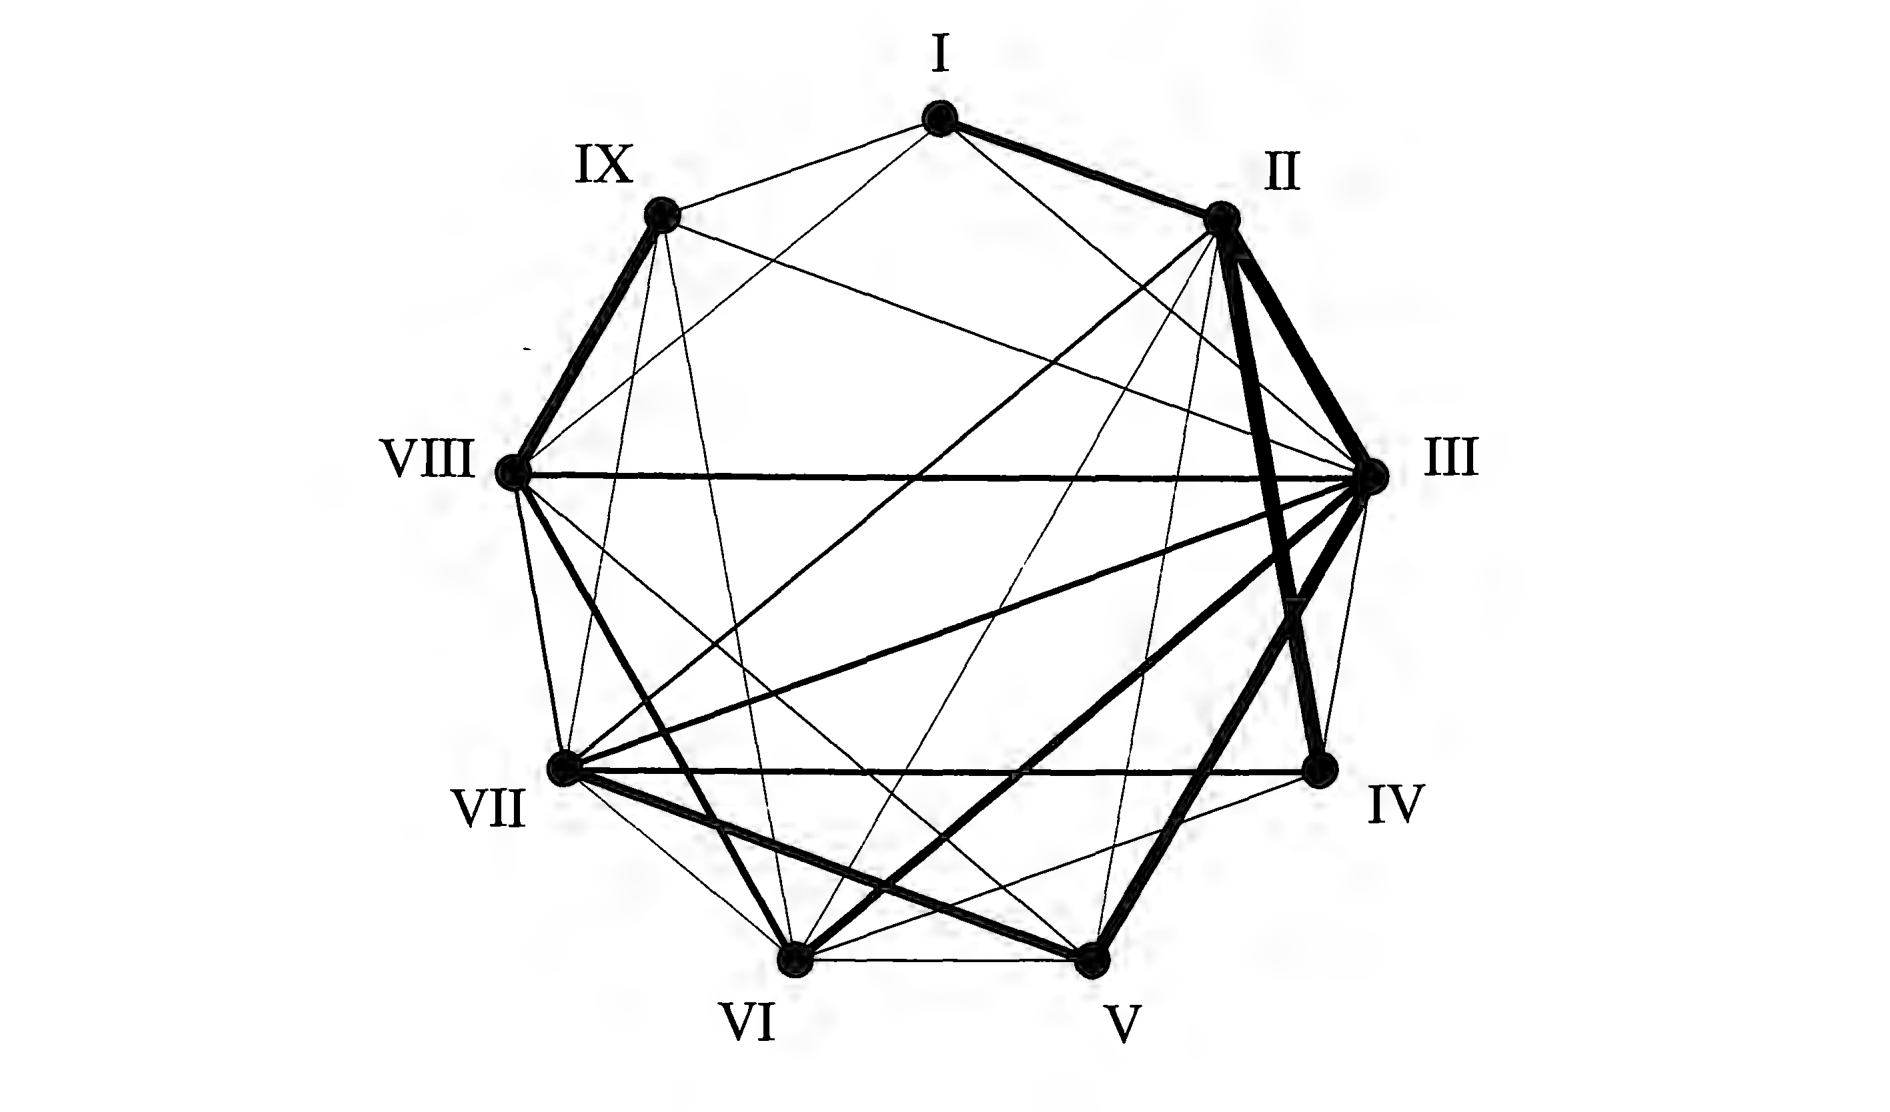
\includegraphics[width=0.62\textwidth]{figs/intro-web.png}
\end{figure}

我特别照顾到了自学的读者, 因而在编制详尽的索引上格外下了一番功夫. 对于一本书的这种篇幅, 不可能为引入的每一个新术语都安排一次正式的``定义''来大事张扬; 索引应当帮助独自旅行的读者找到陌生术语的源头.

书内交叉引用的处理方式希望是透明的. 例如, 注记~III.1.16 指第三章的注记~1.16; 若引用出自第三章内部, 则同一对象就称为注记~1.16. 习题后面方括号中的清单, 列出了书中引用该习题的其他习题或节. 例如, 第一章的习题~3.1 后面跟着 $[\,5.1,\ \S$VIII.1.1$,\ \S$IX.1.2$,\ \text{IX.1.10}\,]$: 这提醒读者, 本题在第一章的习题~5.1、第八章的 \S 1.1、第九章的 \S 1.2 以及第九章的习题~1.10 中被引用 (而且仅在这些地方).

\emph{致谢.} 我对 Lang 的教材~\cite{lang2002algebra}、David Dummit 与 Richard Foote 的 \emph{Abstract Algebra}~\cite{dummitfoote2004abstract} 以及 Michael Artin 的 \emph{Algebra}~\cite{artin1991algebra} 的亏欠, 凡熟悉这些书的人都不难看出. 同调代数那一章则很大程度上得益于 David Eisenbud 的 \emph{Commutative Algebra}~\cite{eisenbud1995commutative} 中论及该主题的附录、Gelfand--Manin 的 \emph{Methods of Homological Algebra}~\cite{gelfandmanin2003methods} 以及 Weibel 的 \emph{An Introduction to Homological Algebra}~\cite{weibel1994introduction}. 但在大多数情形下, 我实在无法追溯某个叙述性的想法、某个证明、某道习题或某种特定的教学侧重最初的来源: 它们多半是这些以及其他有影响的文献中思想的产物, 也常常源于在万维网的万千线索间穿行时触发的联想. 这也是为何我以一种心平气和的精神, 决定基本上完全不列参考文献的另一个原因. 无论如何, 我相信这里呈现的所有材料都是标准的; 对于成品中遗留下来的每一个错误, 我保留绝对的所有权.

我非常感谢我的学生们, 他们持续不断的反馈促使我以这种特定方式写作本书, 并为本书在我课堂上的成功作出了实质性的贡献. 一些学生向我提供了长长的排印错误乃至不折不扣的错误的清单, 我要特别感谢 Kevin Meek、Jay Stryker 与 Yong Jae Cha 极有帮助的意见. $2008$ 年秋, 在 FSU 学术休假期间, 我有机会在 Caltech 的一门课程中试用同调代数的材料, 我感谢 Caltech 以及选课的听众们的热情接待与友好氛围. 也感谢 MSRI 在 $2009$ 年冬天提供的接待, 本书最后的打磨正是在那时完成的.

有几位同行在本书的预备版本中发现了大大小小的错误, 我要提到 Georges Elencwajg、Xia Liao 与 Mirroslav Yotov, 他们的贡献尤为宝贵. 我也要赞扬 Arlene O'Sean 与 AMS 的编辑制作团队出色的文字编辑与制作工作.

特别感谢 Ettore Aldrovandi 的专业建议、Matilde Marcolli 的鼓励与不可或缺的帮助, 以及 Ed Dunne 对本书最终版本的形成影响深远的诸多建议.

本书撰写各阶段所获的 Max-Planck-Institut (Bonn)、NSA 以及 Caltech 的支持, 在此一并致谢.


\mainmatter
% 各章翻译完成后逐一启用:
% 第一章 预备知识: 集合论与范畴 --- 中译
% 原书 pp. 1--40 (Aluffi, Algebra: Chapter 0, Chapter I).
% 本文件进度: §\ref{sec:prelim-naive}--§\ref{sec:universal-properties} 已译 (2026-08-28).

\chapter{预备知识:集合论与范畴}
\label{chap:prelim}


% ===== 记号索引 v1 集中埋点 (页码参考原书书页; 首次出现位置待人工校对) =====
% 本章记号条目（11 条）。OCR 已做最佳校正，但部分符号字形与首次
% 出现位置仍待逐条人工复核（页码沿用原书第 699 页 Index of Notation）。
% ===== /记号索引 =====
\index[sym1]{$An$@$An$}
\index[sym1]{$\Aut_c(A)$@$\Aut_c(A)$}
\index[sym1]{$B^A$@$B^A$}
\index[sym1]{$c$@$c$}
\index[sym1]{$\End_c(A)$@$\End_c(A)$}
\index[sym1]{$\Hom_c(A,B)$@$\Hom_c(A,B)$}
\index[sym1]{$\N$@$\N$}
\index[sym1]{$\mathcal{P}(S)$@$\mathcal{P}(S)$}
\index[sym1]{$\Q$@$\Q$}
\index[sym1]{$\R$@$\R$}
\index[sym1]{$\Z$@$\Z$}
\index{Zermelo@Zermelo!Ernst@Ernst}集合论本身就是数学的一个领域, 而对它的严格处理 (比如说, 通过著名的 Zermelo--Fränkel 公理)
远远超出本书的范围, 也超出笔者的能力. 我们只打算使用所谓的``朴素''集合论%
\index{pusujihelun@朴素集合论(naive set theory)}
, 它不过是一套记号与术语系统, 使我们能够精确地表述数学的定义、命题及其证明.

\index{daishu@代数(algebra)!jiaohuan@交换(commutative)}熟悉这套语言对于学习代数%
\index{daishu@代数(algebra)}
\index{fanchou@范畴(category)!Ab@Ab}这样的学科是必不可少的, 的确, 我们假定读者此前已经接触过它. 在本章中, 我们先回顾朴素集合论语言的一部分, 主要目的是确立全书将使用的记号; 随后我们会对范畴%
\index{fanchou@范畴(category)}
\index{daishu@代数(algebra)!chu@除(division)}的语言略作品尝, 它在代数以及许多其他领域中发挥着强大的统一作用. 我们的主要目标是传达``万有性质''%
\index{wanyouxingzhi@万有性质(universal property)}
的观念, 它将是贯穿全书的一条主线.

\section{朴素集合论}
\label{sec:prelim-naive}

\subsection{集合}
\label{subsec:sets}

集合%
\index{jih@集合(set)}
\index{yuan@元(element)}的概念将``对象的汇集''这一直观想法形式化. 一个集合由它所包含的元素%
\index{yuansu@元素(element)}
确定: 两个集合 $A$, $B$ 相等 (记作 $A = B$) 当且仅当它们包含的元素恰好相同. ``元素是什么?''在朴素集合论中是一个被禁止的问题: 追问必须止于某处. 我们可以方便地假装有一个由元素构成的``宇宙''可供使用, 并从这个宇宙中取材, 构造出我们需要的元素与集合, 同时默认我们将要探索的一切运算都能在这个宇宙中进行. (这正是微妙之处!) 无论如何, 我们通过给出一个确切的规则来确定一个集合, 该规则指明哪些元素在其中. 这样的定义通常写在花括号之间, 也可以是一个元素明确的完整清单:
\[
	A := \{1,2,3\}
\]
\footnote{``:='' 这一记号常用来表示: 左边的符号由右边的内容来定义. 逻辑上这只是在表达两侧的相等, 完全可以直接写``=''; 这个多出来的``:''不过是从计算机科学继承下来的一种心理上方便的装饰.}%
这是由整数 $1$、$2$、$3$ 构成的集合. 按照约定, 列出元素时的次序%
\footnote{有序的清单用圆括号表示: $(1,2,3)$ 与 $(1,3,2)$ 不相同.}%
以及清单中的重复都与定义无关. 于是, 同一个集合可以有许多种写法:
\[
	\{1,2,3\} = \{1,3,2\} = \{1,2,1,3,3,2,3,1,1,2,1,3\}.
\]
\index{yuan@元(element)!Abel fanchouduixiangde@Abel 范畴对象的(of an object of an abelian category)!chudeng@初等(elementary)}这种表示集合的方式可能相当笨拙, 而且无论如何只对有限集真正有效. 对于无限集, 一种流行的变通办法是写出一个清单, 其中某些元素被理解为按某个模式延伸---例如, 偶整数%
\index{ouzhengshu@偶整数(even integer)}
构成的集合可以写成
\[
	E = \{\dots, -2, 0, 2, 4, 6, \dots\},
\]
\index{ji@积(product)!zhi@直(direct)}但这样的定义天然带有歧义, 因而留下误解的空间. 此外, 有些集合简直``太大''了, 即便原则上也无法列出: 例如 (但愿读者在高等微积分中学到过) 实数实在太多, 无法像``列出''整数那样把它们一一``列出''.

更可取的做法往往是: 把集合的元素表达为某个更大的 (并且已知的) 集合 $S$ 中满足某个性质 $P$ 的那些元素 $s$. 这时可以写
\[
	A = \{s \in S \mid s \text{ 满足 } P\}
\]
($\in$ 的意思是``是\ldots 的元素\ldots''), 一般说来这是精确而无歧义的%
\footnote{但要注意, 存在罗素悖论%
\index{luosubeilun@罗素悖论(Russell's paradox)}
这样的病态情形, 它们表明即便这种定义方式也可能导致无意义的结果. 只要 $S$ 本身确实已知是一个集合, 就一切平安无事.}%
.

\index{duozhongji@多重集(multiset)!Sylow dingli@Sylow 定理(Sylow's theorem)}我们偶尔会遇到集合概念的一个变体, 称为``多重集''%
\index{duochongji@多重集(multiset)}
\index{duozhongji@多重集(multiset)!dingli@定理(theorem)}\index{duozhongji@多重集(multiset)!zhangliang@张量(tensor)}\index{duozhongji@多重集(multiset)!Tarski@Tarski!Alfred@Alfred}\index{duozhongji@多重集(multiset)!duichenxing@对称性(symmetry)}\index{duozhongji@多重集(multiset)!duichen@对称(symmetric)}\index{chongshu@重数(multiplicity)!tezhengzhide@特征值的(of an eigenvalue)!jihe@几何(geometry)}\index{chongshu@重数(multiplicity)!tezhengzhide@特征值的(of an eigenvalue)!daishu@代数(algebra)}\index{chongshu@重数(multiplicity)!duoxiangshigende@多项式根的(of a root of a polynomial)}\index{chongshu@重数(multiplicity)}. 多重集是允许元素``带重数地''出现的集合: 也就是说, 在多重集中 $\{2,2\}$ 与 $\{2\}$ 是不同的. 定义多重集的正确方式要借助映射, 我们很快就会遇到 (见例~\ref{subsec:multisets-indexed}).

几个著名的集合:
\begin{itemize}
	\item $\emptyset$: 空集%
\index{kongji@空集(empty set)}
\index{yuan@元(element)!yinzi@因子(divisor)}, 不含任何元素;
	\item $\N$: 自然数集 (即非负整数集);\index[sym1]{42@$\N$}
	\item $\Z$: 整数集;\index[sym1]{68@$\Z$}
	\item $\Q$: 有理数集;\index[sym1]{48@$\Q$}
	\item $\R$: 实数集;\index[sym1]{52@$\R$}
	\item $\CC$: 复数集.\index[sym1]{07@$\CC$}
\end{itemize}
\index{yuan@元(element)!yunsuan@运算(operation)}此外, ``单元素集''%
\index{danyuansuji@单元素集(singleton)}
一词用来指恰由一个元素构成的集合. 于是 $\{1\}$, $\{2\}$, $\{3\}$ 是互不相同的集合, 但它们都是单元素集.

下面是几个有用的符号 (称为量词%
\index{liangci@量词(quantifier)}
):
\begin{itemize}
	\item $\exists$ 表示``存在\ldots'' (存在量词);
	\item $\forall$ 表示``对所有\ldots'' (全称量词).
\end{itemize}
另外, $\exists!$ 用来表示``存在唯一的\ldots''.

例如, 偶整数集可以写成
\[
	E = \{a \in \Z \mid (\exists n \in \Z)\ a = 2n\}:
\]
\index{zi@字(word)}用文字说, ``所有使得存在整数 $n$ 满足 $a = 2n$ 的整数 $a$''. 在这个例子里, 我们可以把 $\exists$ 换成 $\exists!$ 而不改变这个集合---但这与 $\Z$ 的性质有关, 与数学句法无关. 人们还常采用简写
\[
	E = \{2n \mid n \in \Z\},
\]
其中存在量词被默认省略.

能够毫不费力地解析这样的符号串, 并且能够流利地把它们写出来, 是极其重要的. 本书假定读者已经掌握了这一技能.

注意, 书写事物的次序可能带来巨大的差别. 例如, 命题
\[
	(\forall a \in \Z) (\exists b \in \Z) \quad b = 2a
\]
为真: 它说, 把任意整数加倍的结果是整数; 而
\[
	(\exists b \in \Z) (\forall a \in \Z) \quad b = 2a
\]
为假: 它说, 存在一个固定的整数 $b$, 它``同时''是每个整数的两倍---根本没有这种东西.

还要注意, 单独写下
\[
	b = 2a
\]
并不能传达足够的信息, 除非上下文把附着于 $a$ 与 $b$ 的量词交代得完全清楚: 诚如方才所见, 不同的量词可以把同一个式子变成真命题或假命题.

\subsection{集合的包含}
\label{subsec:inclusion}

如前所述, 两个集合相等当且仅当它们包含相同的元素. 我们说集合 $S$ 是集合 $T$ 的子集%
\index{ziji@子集(subset)}
, 如果 $S$ 的每个元素都是 $T$ 的元素, 用符号写成
\[
	S \subseteq T.
\]
按照约定, $S \subset T$ 的含义相同: 也就是说 (与 $<$ 对 $\leq$ 的情形不同), 它不排除 $S$ 与 $T$ 相等的可能. 为避免任何混淆, 本书将一致地使用 $\subseteq$. 我们用 $S \subsetneq T$ 表示 $S$``真''含于 $T$: 即 $S \subseteq T$ 且 $S \neq T$.

可以用逻辑的语言来考虑``集合的包含'': $S \subseteq T$ 意味着
\[
\index{Lie@Lie!Sophus@Sophus}	s \in S \implies s \in T
\]
(量词 $\forall s$ 默认省略); 也就是说, ``若 $s$ 是 $S$ 的元素, 则 $s$ 是 $T$ 的元素''; 也就是说, $S$ 的所有元素都是 $T$ 的元素; 也就是说, 正如所许, $S \subseteq T$.

注意, 对所有集合 $S$, 有 $\emptyset \subseteq S$ 且 $S \subseteq S$.

若 $S \subseteq T$ 且 $T \subseteq S$, 则 $S = T$.

符号 $|S|$ 表示 $S$ 的元素个数 (当这个数有限时); 否则记 $|S| = \infty$. 若 $S$ 与 $T$ 有限, 则
\[
\index{Lie@Lie!Sophus@Sophus!daishu@代数(algebra)}	S \subseteq T \implies |S| \leq |T|.
\]
一个集合 $S$ 的全体子集构成一个集合, 称为 $S$ 的幂集%
\index{miji@幂集(power set)}
\index{juzhendexingkongjian@矩阵的行空间(row space of a matrix)}\index{juzhendexingkongjian@矩阵的行空间(row space of a matrix)!huan@环(ring)}\index{mi@幂(power)!ziyu@子域(subfield)!bukeyue@不可约(irreducible)}\index{mi@幂(power)!feilinglixiangzai PID zhongjida@非零理想在 PID 中极大(nonzero ideals are maximal in a PID)!bukeyue@不可约(irreducible)}\index{mi@幂(power)!lixiang@理想(ideal)!bukeyue@不可约(irreducible)}\index{mi@幂(power)!zhenghuanzhongdeyuan@整环中的元(element in an integral domain)!bukeyue@不可约(irreducible)}\index{mi@幂(power)!xiangban@相伴(associated)!mode@模的(of a module)!bukeyue@不可约(irreducible)}\index{mi@幂(power)!jishu@级数(series)!bukeyue@不可约(irreducible)}\index{mi@幂(power)!jishu@级数(series)}\index{mi@幂(power)}(或``部分集合之集''). 例如, 空集 $\emptyset$ 的幂集由一个元素构成: $\{\emptyset\}$. $S$ 的幂集记作 $\mathcal{P}(S)$; 常见的替代记号是 $2^S$, 而且当 $S$ 有限时确有 $|\mathcal{P}(S)| = 2^{|S|}$ (参见习题~\ref{ex:two-to-power}).\index[sym1]{45@$\mathcal{P}(S)$}

\subsection{集合间的运算}
\label{subsec:operations}

手头有了几个集合之后, 就可以通过某些标准运算得到更多的集合. 这里有几个:
\begin{itemize}
	\item $\cup$: 并;
	\item $\cap$: 交;
	\item $\smallsetminus$: 差;
	\item $\amalg$: 无交并%
\index{wujiaobing@无交并(disjoint union)}
;
	\item $\times$: (Cartesian) 积%
\index{jij@积(product)}
;
	\item 以及``模等价关系取商''这一重要概念.
\end{itemize}
这些运算中的大多数读者应当已经熟悉: 例如,
\[
	\{1,2,4\} \cup \{3,4,5\} = \{1,2,3,4,5\},
\]
而
\[
	\{1,2,4\} \smallsetminus \{3,4,5\} = \{1,2\}.
\]
用令人回忆起臭名昭著的``新数学''的维恩图%
\index{weientu@维恩图(Venn diagram)}
表示如下:
\index{zhongxin@中心(center)!huande@环的(of a ring)}\index{zhongxin@中心(center)!qunde@群的(of a group)}\begin{center}
\begin{tikzpicture}[scale=0.72,line width=0.5pt]
\begin{scope}
\draw[pattern=north east lines] (0,0) ellipse (1.5 and .85);
\draw[pattern=north west lines] (1.7,0) ellipse (1.5 and .85);
\node at (-2.1,.7) {$S$}; \node at (3.8,.7) {$T$};
\end{scope}
\foreach \x/\opname in {-5.4/{S\cup T},.85/{S\cap T},7.1/{S\smallsetminus T}} {
\begin{scope}[shift={(\x,-4.2)}]
\draw[pattern=north east lines] (0,0) ellipse (1.5 and .85);
\draw[pattern=north west lines] (1.7,0) ellipse (1.5 and .85);
\node at (.85,-1.5) {$\opname$};
\end{scope}}
\begin{scope}[shift={(-5.4,-4.2)}]
\draw[line width=1.6pt] ({1.5*cos(55.48)},{.85*sin(55.48)}) arc[start angle=55.48,end angle=304.52,x radius=1.5,y radius=.85];
\draw[line width=1.6pt] ({1.7+1.5*cos(235.48)},{.85*sin(235.48)}) arc[start angle=235.48,end angle=484.52,x radius=1.5,y radius=.85];
\end{scope}
\begin{scope}[shift={(.85,-4.2)}]
\draw[line width=1.6pt] ({1.5*cos(-55.48)},{.85*sin(-55.48)}) arc[start angle=-55.48,end angle=55.48,x radius=1.5,y radius=.85];
\draw[line width=1.6pt] ({1.7+1.5*cos(124.52)},{.85*sin(124.52)}) arc[start angle=124.52,end angle=235.48,x radius=1.5,y radius=.85];
\end{scope}
\begin{scope}[shift={(7.1,-4.2)}]
\draw[line width=1.6pt] ({1.5*cos(55.48)},{.85*sin(55.48)}) arc[start angle=55.48,end angle=304.52,x radius=1.5,y radius=.85];
\draw[line width=1.6pt] ({1.7+1.5*cos(235.48)},{.85*sin(235.48)}) arc[start angle=235.48,end angle=124.52,x radius=1.5,y radius=.85];
\end{scope}
\end{tikzpicture}
\end{center}
(其中黑色实线轮廓指明了参与该运算的集合).

其中几种运算可以用逻辑语言透明地写出: 例如,
\[
	s \in S \cap T \iff (s \in S \ \text{ 并且 } \ s \in T).
\]
两个集合 $S$ 与 $T$ 称为不相交%
\index{buxiangjiao@不相交(disjoint)}
, 如果 $S \cap T = \emptyset$, 也就是说, 没有``同时''属于二者的元素.

子集 $T$ 在集合 $S$ 中的补集%
\index{buji@补集(complement)}
是差集 $S \smallsetminus T$, 它由 $S$ 中所有不在 $T$ 中的元素构成. 例如, 偶整数集在 $\Z$ 中的补集就是奇整数集.

运算 $\amalg$, $\times$ 以及模等价关系取商则稍微神秘一些, 仔细琢磨它们是极有教益的. 我们将先以特别朴素的方式考察它们, 待获得了更多语言、能够从更成熟的视角审视它们之后, 再回过头来讨论.

\subsection{无交并、积}
\index{ji@积(product)!mode@模的(of a module)}\index{ji@积(product)!qunde@群的(of a group)}\index{ji@积(product)!zai Abel fanchouzhong@在 Abel 范畴中(in an abelian category)}\index{ji@积(product)!ziyou@自由(free)}\index{ji@积(product)!xianwei@纤维(fiber)}\label{subsec:disjoint-unions-products}

这些运算有一个问题: 它们的输出可能无法定义为一个集合, 而只能定义为一个``相差集合之同构意义上的''集合, 也就是说, 相差双射意义上的集合. 要把这话说清楚, 就必须谈论映射; 我们马上就来做这件事.

粗略地说, 两个集合 $S$ 与 $T$ 的无交并是一个集合 $S \amalg T$, 它这样得到: 先造出 $S$ 与 $T$ 的``副本'' $S'$ 与 $T'$, 满足 $S' \cap T' = \emptyset$, 然后取 $S'$ 与 $T'$ 的 (普通) 并. 细心的读者会感到不安, 因为这份``配方''并未定义出一个集合: 无论``造一个集合的副本''是什么意思, 肯定有许多种造法. 这一歧义将在下文澄清.

尽管如此, 请注意, 即便在这样站不住脚的基础上, 关于 $S \amalg T$ 我们仍能说点什么: 例如, 若 $S$ 由 $3$ 个元素组成, $T$ 由 $4$ 个元素组成, 那么读者应当 (而且能够正确地) 期望 $S \amalg T$ 由 $7$ 个元素组成.

积也被同样类型的歧义所困扰, 但幸运的是有一个方便的约定, 使我们能够写下代表两个集合 $S$ 与 $T$ 之积的``某一个''集合: 给定 $S$ 与 $T$, 我们令 $S \times T$ 为由 $S$ 与 $T$ 的元素构成的有序对%
\index{youxudui@有序对(ordered pair)}
$(s,t)$ 组成的集合%
\footnote{有序对 $(s,t)$ 可以用集合来定义: 令 $(s,t) = \{s, \{s,t\}\}$. 这样既携带了元素 $s$ 与 $t$ 的信息, 又表达了 $s$ 的特殊地位 (= 序对的第一个元素).}%
:
\[
	S \times T := \{(s,t) \text{ 使得 } s \in S,\ t \in T\}.
\]
于是, 若 $S = \{1,2,3\}$, $T = \{3,4\}$, 则
\[
	S \times T = \{(1,3), (1,4), (2,3), (2,4), (3,3), (3,4)\}.
\]
一个更精致的例子: $\R \times \R$ 是实数对的集合, 它 (正如读者在微积分中学到的) 是平面的一种很好的表示. 集合 $\Z \times \Z$ 则可以表示为这个平面中恰好具有整数坐标的那些点. 顺便一提, 人们常把这两个集合记作 $\R^2$, $\Z^2$; 类似地, 集合与其自身的积 $A \times A$ 常记作 $A^2$.

若 $S$ 与 $T$ 是有限集, 则显然 $|S \times T| = |S|\,|T|$.

还应注意, 我们可以用积来按需造出无交并所需的``副本'': 例如, 可以令 $S' = \{0\} \times S$, $T' = \{1\} \times T$, 这就保证了 $S'$ 与 $T'$ 不相交 (为什么?); 并且有一种明显的方式去``认同'' $S$ 与 $S'$、$T$ 与 $T'$. 再说一遍, 把这话说精确还需要一点词汇.

运算 $\cup$, $\cap$, $\amalg$, $\times$ 可以推广到整``族''集合上的运算: 例如, 若 $S_1, \ldots, S_n$ 是集合, 我们写
\[
\bigcap_{i=1}^{n} S_i = S_1 \cap S_2 \cap \dots \cap S_n
\]
表示由那些同时是 $S_1, \ldots, S_n$ 中每一个集合的元素组成的集合; 其他运算类似. 但请注意, 虽然从定义看显然有
\[
S_1 \cup S_2 \cup S_3 = (S_1 \cup S_2) \cup S_3 = S_1 \cup (S_2 \cup S_3),
\]
但
\[
S_1 \times S_2 \times S_3, \quad (S_1 \times S_2) \times S_3, \quad S_1 \times (S_2 \times S_3)
\]
这些集合应当在何种意义上被``认同'', 却不那么清楚 (此时最左边的集合可以仿照两个集合的情形, 定义为由 $S_1$, $S_2$, $S_3$ 中元素构成的``有序三元组''之集). 事实上, 又一次地, 只有在掌握了映射的语言之后, 我们才能真正理解这类陈述. 不过, 正如读者大概期望的那样, 所有这类陈述最终都被证实为真; 由于这一幸运的情况, 我们可以稍稍随便一些, 对这类微妙之处一笔带过.

更一般地, 若 $\mathcal{S}$ 是一个由集合构成的集合, 我们可以考虑
\[
\bigcup_{S \in \mathcal{S}} S, \quad \bigcap_{S \in \mathcal{S}} S, \quad \coprod_{S \in \mathcal{S}} S, \quad \prod_{S \in \mathcal{S}} S,
\]
即 $\mathcal{S}$ 中所有集合的并、交、无交并与积. 这些定义涉及一些重要的微妙之处: 例如, 若所有 $S \in \mathcal{S}$ 都非空, 是否能推出 $\prod_{S \in \mathcal{S}} S$ 非空? 读者大概认为是显然的, 但 (若 $\mathcal{S}$ 无限) 这是相当棘手的问题, 它等价于选择公理%
\index{xuanzegongli@选择公理(axiom of choice)}
.

大体而言, 这些微妙之处并不影响本课程的内容; 待它们与手头的问题变得更为相关时, 我们会 (在 \S V.\ref{sec:zorn-lemma}) 部分地与它们和解%
\footnote{读者在此后的若干习题中将时不时需要动用选择公理, 即便在我们回头讨论这些问题之前也是如此; 但这多半会发生在觉察阈值之下, 而这恰恰是它应有的样子.}%
.

\subsection{等价关系、划分、商}
\index{guanxi@关系(relation)!jie@阶(order)}\index{guanxi@关系(relation)!dengjia@等价(equivalence)}\index{guanxi@关系(relation)!yuqunjiegouxiangrong@与群结构相容(compatible with a group structure)}\label{subsec:equivalence-relations}

直观地说, 一个集合 $S$ 的元素之间的关系%
\index{guanxi@关系(relation)}
, 是 $S$ 的元素的某些选择之间的某种特殊亲缘. 例如, $\Z$ 上的关系 $<$ 是比较两个整数大小的方式: 由于 $2 < 5$, 在这个意义下 $2$``与''$5$ 有关系, 而 $5$ 在同一意义下与 $2$ 没有关系.

就一切实用目的而言, 一个关系``意指''什么, 完全由集合中哪些元素与哪些元素有关系所刻画. 如果我们拥有一份由所有使得 $a < b$ 的整数对 $(a,b)$ 组成的完整清单, 那么关于 $\Z$ 上的 $<$ 我们就无所不知了. 例如, $(2,5)$ 是这样的一对, 而 $(5,2)$ 不是.

这就引出了关系概念的完全直截了当的定义: 集合 $S$ 上的关系就是积 $S \times S$ 的一个子集 $R$. 若 $(a,b) \in R$, 我们说 $a$ 与 $b$ ``有关系 $R$'', 并写作
\[
a \mathrel{R} b.
\]
人们常为关系使用更花哨的符号, 诸如 $<$, $\leq$, $=$, $\sim$, \ldots.

性质良好的关系的原型是``='', 它对应于``对角线''
\[
\{(a,b) \in S \times S \mid a = b\} = \{(a,a) \mid a \in S\} \subseteq S \times S.
\]
这个非常特殊的关系的三条性质被证明是特别重要的: 若暂时用 $\sim$ 记相等关系 $=$, 则 $\sim$ 满足
\begin{itemize}
	\item 自反性: $(\forall a \in S)\ a \sim a$;
	\item 对称性: $(\forall a \in S) (\forall b \in S)\ a \sim b \implies b \sim a$;
	\item 传递性: $(\forall a \in S) (\forall b \in S) (\forall c \in S),\ (a \sim b \text{ 并且 } b \sim c) \implies a \sim c$.
\end{itemize}
也就是说, 每个 $a$ 都等于它自身; 若 $a$ 等于 $b$, 则 $b$ 等于 $a$; 等等.

\begin{definition}[等价关系]
\label{def:equiv-rel}
集合 $S$ 上的等价关系%
\index{dengjiaguanxi@等价关系(equivalence relation)}
是指满足上述三条性质的任意关系 $\sim$.
\end{definition}

用 $S \times S$ 中相应的子集 $R$ 的语言来说, ``自反性''说的是对角线包含于 $R$; ``对称性''说的是 $R$ 关于对角线翻转不变 (即每个 $(a,b)$ 换成 $(b,a)$); 而遗憾的是, ``传递性''没有同样漂亮的图示翻译.

$S$ 上的等价关系这一数据, 结果等价于一类乍看之下稍有不同的信息, 即 $S$ 的一个划分%
\index{huafen@划分(partition)}
. $S$ 的划分是 $S$ 的一族两两不交的非空子集, 其并为 $S$: 例如,
\[
\mathscr{P} = \{\{1,4,7\}, \{2,5,8\}, \{3,6\}, \{9\}\}
\]
是集合
\[
\{1,2,3,4,5,6,7,8,9\}
\]
的一个划分.

以下是如何从 $S$ 上的关系 $\sim$ 得到 $S$ 的一个划分: 对每个元素 $a \in S$, $a$ 的 (相对于 $\sim$ 的) 等价类%
\index{dengjialei@等价类(equivalence class)}
是 $S$ 的子集
\[
[a]_{\sim} := \{b \in S \mid b \sim a\};
\]
于是这些等价类构成 $S$ 的一个划分 $\mathscr{P}_{\sim}$ (习题~\ref{ex:partition-from-relation}).

反之 (习题~\ref{ex:relation-from-partition}), 每个划分 $\mathscr{P}$ 都以这种方式对应于某个等价关系. 因此, ``$S$ 上的等价关系''与``$S$ 的划分''这两个概念实质上是等价的.

现在我们可以把 $\mathscr{P}_{\sim}$ 视为一个集合 (其元素是相对于 $\sim$ 的等价类). 这就是 \S\ref{subsec:operations} 中提到的取商运算.

\begin{definition}[商]
\label{def:quotient}
集合 $S$ 关于等价关系 $\sim$ 的商%
\index{shangji@商(quotient)}
是 $S$ 的元素相对于 $\sim$ 的等价类之集
\[
S / {\sim} := \mathscr{P}_{\sim}.
\]
\end{definition}

\begin{example}
\label{ex:mod-two}
取 $S = \Z$, 并令 $\sim$ 为由
\[
a \sim b \iff a - b \text{ 是偶数}
\]
定义的关系. 则 $\Z / {\sim}$ 由两个等价类构成:
\[
\Z / {\sim} = \{[0]_{\sim}, [1]_{\sim}\}.
\]
的确, 每个整数 $b$ 要么是偶数 (从而 $b - 0$ 是偶数, 故 $b \sim 0$, 即 $b \in [0]_{\sim}$), 要么是奇数 (从而 $b - 1$ 是偶数, 故 $b \sim 1$, 即 $b \in [1]_{\sim}$). 这当然是模算术的起点, 稍后我们将对它作应尽的详细介绍 (\S II.\ref{subsec:cyclic-groups}).

思考这一运算的一种方式是: 等价关系在商中``变成相等'': 也就是说, 商 $S/{\sim}$ 中的两个元素相等, 当且仅当 $S$ 中相应的元素有关系 $\sim$. 换言之, 取商是一种把任意等价关系变成相等关系的办法. 这一观察稍后将在``范畴的语言''中进一步形式化 (\S\ref{subsec:quotients-up}).
\end{example}

\subsection*{习题}
\phantomsection
\addcontentsline{toc}{subsection}{习题}

标有 $\triangleright$ 的习题被正文引用; 标有 $\neg$ 的习题被其他习题引用. 引用它们的习题与节列在该习题后面的方括号中; 如有必要, 请参阅前言中的进一步说明.

\begin{prob}
\label{ex:russell}
查找关于罗素悖论的讨论, 并把它弄懂.
\end{prob}

\begin{prob}
\label{ex:partition-from-relation}
$\triangleright$ 证明: 若 $\sim$ 是集合 $S$ 上的一个等价关系, 则 \S\ref{subsec:equivalence-relations} 中定义的相应族 $\mathscr{P}_{\sim}$ 确实是 $S$ 的一个划分: 也就是说, 其元素非空、两两不交, 且其并为 $S$. [\S\ref{subsec:equivalence-relations}]
\end{prob}

\begin{prob}
\label{ex:relation-from-partition}
$\triangleright$ 给定集合 $S$ 上的一个划分 $\mathscr{P}$, 说明如何在 $S$ 上定义一个等价关系\erratumfootnote{根据官方勘误, 此处应为``等价关系''(equivalence relation).} $\sim$, 使得 $\mathscr{P}$ 正是与之相应的划分. [\S\ref{subsec:equivalence-relations}]
\end{prob}

\begin{prob}
\label{ex:equiv-rel-123}
在集合 $\{1,2,3\}$ 上可以定义多少个不同的等价关系?
\end{prob}

\begin{prob}
\label{ex:refl-symm-not-trans}
给出一个自反且对称但不传递的关系的例子. 如果试图用这个关系在集合上定义划分, 会发生什么? (提示: 思考第二个问题将有助于回答第一个问题.)
\end{prob}

\begin{prob}
\label{ex:quotient-R}
$\triangleright$ 在实数集 $\R$ 上定义关系 $\sim$: 规定 $a \sim b \iff b - a \in \Z$. 证明这是一个等价关系, 并对 $\R / {\sim}$ 找出一个``令人信服''的描述. 对平面 $\R \times \R$ 上通过规定 $(a_1, a_2) \approx (b_1, b_2) \iff b_1 - a_1 \in \Z$ 且 $b_2 - a_2 \in \Z$ 定义的关系 $\approx$ 做同样的事情. [\S~II.\ref{subsec:canon-quotient}, II.\ref{ex:torus}]
\end{prob}

\section{集合间的映射}
\label{sec:functions}

\subsection{定义}
\label{subsec:functions-def}

对于本书引入的几乎每一种结构, 我们都将遵循一条共同的主线: 既设法理解这种结构本身, 也理解这种结构的不同实例之间可能如何相互作用.

集合通过映射%
\index{yingshe@映射(map)}
相互作用. 人们难免想用``动态''的措辞来思考从集合 $A$ 到集合 $B$ 的映射 $f$, 把它当作``从 $A$ 走到 $B$''的一种方式. 与关系的情形类似, 把这个概念形式化而无需求助任何给定 $f$ 的深层``含义''是直截了当的: 关于映射 $f$ 可以知道的一切, 都被如下信息所刻画, 即 $A$ 中任一给定元素 $a$ 的像是 $B$ 中哪个元素 $b$. 这个信息不过是 $A \times B$ 的一个子集:
\[
\Gamma_f := \{(a,b) \in A \times B \mid b = f(a)\} \subseteq A \times B.
\]
集合 $\Gamma_f$ 称为 $f$ 的图像%
\index{tuxiang@图像(picture)}
; 严格地说, 映射``就是''它的图像%
\footnote{更精确地说, 是图像 $\Gamma_f$ 连同 $f$ 的源 $A$ 与目标 $B$ 的信息; 这些都属于映射的数据的一部分.}%
.

并非 $A \times B$ 的所有子集 $\Gamma \subseteq A \times B$ 都对应于 (即``是'') 映射: 我们需要对映射的图像施加一条要求, 它可以表述如下:
\[
(\forall a \in A) (\exists! b \in B)\ (a,b) \in \Gamma_f,
\]
或者 (``用函数记号'')
\[
(\forall a \in A) (\exists! b \in B)\ f(a) = b.
\]
也就是说, 映射必须把 $A$ 的每个元素 $a$ 送到 $B$ 的恰好一个元素, 而且该元素依赖于 $a$. 诸如 $\pm\sqrt{x}$ 这样的``多值函数'' (它们在, 比如, Riemann 面的研究中非常重要) 在这个意义下不是映射.

要宣布 $f$ 是从集合 $A$ 到集合 $B$ 的映射, 就写 $f : A \to B$, 或画出下图 (``图''):
\[
A \xrightarrow{f} B.
\]
映射 $f : A \to B$ 在元素 $a \in A$ 上的作用有时用一个``带装饰的''箭头表示, 如
\[
a \mapsto f(a).
\]
从一个集合 $A$ 到一个集合 $B$ 的所有映射的汇集本身也是一个集合%
\footnote{这是另一种``集合间的运算'', 未列在 \S\ref{subsec:operations} 中. 你能看出我们为什么把这个集合记作 $B^A$ 吗? (参见习题~\ref{ex:card-ba}.)}\index[sym1]{06@$B^A$}%
, 记作 $B^A$. 如果我们认真对待``映射其实与它的图像是同一回事''这一观念, 那么可以把 $B^A$ 视为 $A \times B$ 的幂集的一个 (特殊) 子集.

每个集合 $A$ 都自带一个非常特殊的映射, 其图像是 $A \times A$ 中的对角线: $A$ 上的恒同映射%
\index{hengtong@恒同(identity)}
\[
\id_A : A \to A
\]
由 $(\forall a \in A)\ \id_A(a) = a$ 定义. 更一般地, 集合 $A$ 的任意子集 $S$ 的包含关系确定一个映射 $S \to A$, 它把 $S$ 的每个元素 $s$ 送到 $A$ 中``它自己''.

若 $S$ 是 $A$ 的子集, 我们用 $f(S)$ 表示 $B$ 的子集
\[
f(S) := \{b \in B \mid (\exists a \in S)\ b = f(a)\}.
\]
也就是说, $f(S)$ 是 $B$ 的由 $S$ 的元素在映射 $f$ 下的全部像组成的子集. 其中最大者, 即 $f(A)$, 称为 $f$ 的像%
\index{xiang@像(image)}
, 记作``$\Image f$''.

另外, $f|_S$ 表示 $f$ 在子集 $S$ 上的``限制''%
\index{xianzhi@限制(restriction)}
: 这是映射 $S \to B$, 定义为
\[
(\forall s \in S): \quad f|_S(s) = f(s).
\]
也就是说, $f|_S$ 是复合 (按下一小节解释的意义) $f \circ i$, 其中 $i : S \to A$ 是包含映射. 注意 $f(S) = \Image (f|_S)$.

\subsection{例子: 多重集、加标集合}
\label{subsec:multisets-indexed}

\S\ref{subsec:sets} 中简略提到的``多重集''是借助映射容易形式化的概念的一个简单例子. 多重集可以这样定义: 给定一个从 (普通) 集合 $A$ 到正%
\index{xianxingbianhuandetezhengzhi@线性变换的特征值(eigenvalue of a linear transformation)}\index{xianxingbianhuandetezhengzhi@线性变换的特征值(eigenvalue of a linear transformation)!dechongshu@的重数(multiplicity of)}\footnote{一些文献允许 $0$ 作为可能的重数.}%
整数集 $\N^*$ 的映射; 若 $m : A \to \N^*$ 是这样一个映射, 相应的多重集由元素 $a \in A$ 组成, 每个元素取 $m(a)$ 次. 于是, 多重集 $\{a,a,a,b,b,b,b,b,c\}$ 实质上就是满足 $m(a) = 3$, $m(b) = 5$, $m(c) = 1$ 的映射 $m : \{a,b,c\} \to \N^*$. 与普通集合一样, 元素列出的次序不属于多重集所携带的信息. 包含、并等简单的集合论概念可以直截了当地推广到多重集. 关于多重集的另一种观点, 见习题~\ref{ex:mset-category}.

另一个例子是``指标''的使用. 如果我们写``令 $a_1, \ldots, a_n$ 为整数\ldots'', 我们真正的意思是``考虑一个映射 $a : \{1, \ldots, n\} \to \Z$ \ldots'', 并理解 $a_i$ 是值 $a(i)$ 的简写 (对 $i = 1, \ldots, n$). 人们难免把加标集合%
\index{jiabiaojih@加标集合(indexed set)}
$\{a_i\}_{i \in I}$ 简单地想成一个集合, 其元素恰好被记作 $a_i$, 而 $i$ 取遍某个``指标集'' $I$; 但这样的加标集合更严格地说是一个映射 $I \to A$, 其中 $A$ 是某个我们从中提取元素 $a_i$ 的集合. 例如, 这使得我们可以把 $a_0$ 与 $a_1$ 视为 $\{a_i\}_{i \in \N}$ 的两个不同元素, 即便碰巧作为目标集合 $A$ 的元素有 $a_0 = a_1$.

\index{xiangliang@向量(vector)!cong@丛(bundle)}这类微妙之处很容易被忽视, 而且记号上的某些滥用是常见的、通常也是无害的. 这些区分在 (例如) 关于向量组%
\index{xiangliangzu@向量组(vectors)}
\index{xianxing（wu）guan@线性（无）关(linearly dependent/independent)}\index{xianxing@线性(linear)}线性无关%
\index{xianxingwuguan@线性无关(linearly independent)}
的讨论中起作用; 参见 \S VI.\ref{subsec:linear-independence-bases}.

\subsection{映射的复合}
\label{subsec:composition}

映射可以复合: 若 $f : A \to B$ 与 $g : B \to C$ 是映射, 则由
\begin{equation*}
(\forall a \in A) \quad (g \circ f)(a) := g(f(a)) \tag{$*$}
\end{equation*}
定义的运算 $g \circ f$ 也是映射. 也就是说, 我们先利用 $f$ 从 $A$ 到 $B$, 再应用 $g$ 到达 $C$. 用图形可以画出诸如
\[
\begin{tikzcd}[column sep=large]
A \ar[r,"f"] \ar[rr,bend right=25,"g\circ f"'] & B \ar[r,"g"] & C
\end{tikzcd}
\qquad\text{或}\qquad
\begin{tikzcd}
& B \ar[dr,"g"] & \\
A \ar[ur,"f"] \ar[rr,"g\circ f"'] & & C
\end{tikzcd}
\]
的图. 用这种图形表示 (比如) 由映射相连的集合的汇集, 称为图%
\index{tu@图(graph)}
. 我们将画许多图, 而且是在比眼下这个语境一般得多的语境中.

我们说上面画的图``交换'', 或``是交换的''%
\index{jiaohuantu@交换图(commutative diagram)}
, 意思是: 若我们从 $A$ 出发, 沿图中规定的两种可能路径之一走到 $C$, 沿途应用所遇到的映射, 得到的结果相同. 这恰恰就是陈述 $(*)$ 的内容.

复合是结合的: 也就是说, 若 $f : A \to B$, $g : B \to C$, $h : C \to D$ 是映射, 则 $h \circ (g \circ f) = (h \circ g) \circ f$. 用图形表示, 图
\begin{center}
\begin{tikzcd}[column sep=1.6em]
	A \ar[r, "f"] \ar[rr, bend right=22, "g \circ f"'] & B \ar[r, "g"] \ar[rr, bend left=22, "h \circ g"] & C \ar[r, "h"] & D
\end{tikzcd}
\end{center}
交换. 从复合的定义看, 这个重要的观察应当是完全显然的.

恒同映射关于复合是非常特殊的: 若 $f : A \to B$ 是任意映射, 则 $\id_B \circ f = f$ 且 $f \circ \id_A = f$. 用图形表示, 图
\[
\begin{tikzcd}[column sep=large]
A \ar[r,"f"] \ar[rr,bend right=25,"f"'] & B \ar[r,"\id_B"] & B
\end{tikzcd}
\qquad
\begin{tikzcd}[column sep=large]
A \ar[r,"\id_A"] \ar[rr,bend right=25,"f"'] & A \ar[r,"f"] & B
\end{tikzcd}
\]
交换.

\subsection{单射、满射、双射}
\label{subsec:inj-surj-bij}

有几类特殊的映射值得突出标出:
\begin{itemize}
	\item 映射 $f : A \to B$ 称为单的%
(或单射%
\index{danshe@单射(injective)}
, 或一对一), 如果
	\[
\index{Lie@Lie!Sophus@Sophus!kuohao@括号(bracket)}	a' \neq a'' \implies f(a') \neq f(a''):
	\]
	也就是说, $f$ 把不同的元素送到不同的元素%
	\footnote{人们常用逆否 (因而等价) 的形式来检验这个定义, 即 $(\forall a' \in A)(\forall a'' \in A)\ f(a') = f(a'') \implies a' = a''$.}%
	.

	\item 映射 $f : A \to B$ 称为满的%
\index{mande@满的(full)}
(或满射%
\index{manshe@满射(surjective)}
, 或映上), 如果
	\[
	(\forall b \in B) (\exists a \in A) \quad b = f(a):
	\]
	也就是说, $f$``覆盖整个 $B$''; 更精确地说, $\Image f = B$.
\end{itemize}
单射常画作 $\hookrightarrow$; 满射常画作 $\twoheadrightarrow$.

若 $f$ 既是单的又是满的, 就称它是双射%
\index{shuangshe@双射(bijective)}
(或一一对应, 或集合之同构%
\index{tonggou@同构(isomorphism)}
). 这时我们常写 $f : A \xrightarrow{\sim} B$, 或
\[
A \cong B,
\]
并说 $A$ 与 $B$ 是``同构''的集合.

当然, 恒同映射 $\id_A : A \to A$ 是双射.

若 $A \cong B$, 即存在双射 $f : A \to B$, 则集合 $A$ 与 $B$ 可以通过 $f$ 被``认同'', 意思是我们能把 $A$ 的元素 $a$ 与 $B$ 中相应的元素 $f(a)$ 精确地匹配起来. 例如, 若 $A$ 是有限集且 $A \cong B$, 则 $B$ 必然也是有限集, 且 $|A| = |B|$.

有了这套术语, 我们就能更好地理解 \S\ref{subsec:operations} 中关于``无交并''的讨论: 所给集合 $A$, $B$ 的``副本'' $A'$, $B'$ 就应当分别是与 $A$, $B$ 同构的集合. \S\ref{subsec:disjoint-unions-products} 末尾提出的制造这种不交``副本''的方案是可行的, 因为 (比如) 由
\[
(\forall a \in A) \quad f(a) = (0, a)
\]
定义的
\[
f : A \to \{0\} \times A
\]
显然是双射.

\subsection{单射、满射、双射: 第二种观点}
\label{subsec:second-viewpoint}

思考这些概念还有另一种富有启发性的方式.

若 $f : A \to B$ 是双射, 则可以``把它的图像翻转'', 定义一个映射
\[
g : B \to A:
\]
也就是说, 恰当 $b = f(a)$ 时规定 $a = g(b)$. ($f$ 既单又满这一事实保证了 $\Gamma_f$ 的翻转按 \S\ref{subsec:functions-def} 给出的定义是某个映射的图像. 请自行验证!)

这个映射 $g$ 有一个非常有趣的性质: 用图形表示,
\[
\begin{tikzcd}[column sep=large]
A \ar[r,"f"] \ar[rr,bend right=25,"\id_A"'] & B \ar[r,"g"] & A
\end{tikzcd}
\qquad
\begin{tikzcd}[column sep=large]
B \ar[r,"g"] \ar[rr,bend right=25,"\id_B"'] & A \ar[r,"f"] & B
\end{tikzcd}
\]
交换; 也就是说, $g \circ f = \id_A$ 且 $f \circ g = \id_B$. 第一个等式告诉我们 $g$ 是 $f$ 的``左逆''%
\footnote{别管在图中 $g$ 被画在 $f$ 的右边这件事---我们说 $g$ 是 $f$ 的左逆, 是因为它写在 $f$ 的左边: $g \circ f = \id_A$.}%
; 第二个等式告诉我们 $g$ 是 $f$ 的``右逆''. 我们干脆说它是 $f$ 的逆%
\index{nid@逆(inverse)}
, 记作 $f^{-1}$. 于是, ``双射有逆''.

\index{ni@逆(inverse)!shiweiyide@是唯一的(is unique)}那逆命题呢? 若一个映射有逆, 它是双射吗? 这是真的, 而且事实上我们能说得精确得多.

\begin{proposition}
\label{prop:left-right-inverse}
设 $A \neq \emptyset$, 并设 $f : A \to B$ 是映射. 则
\begin{enumerate}
	\item $f$ 有左逆当且仅当它是单的;
	\item $f$ 有右逆当且仅当它是满的.
\end{enumerate}
\end{proposition}

\begin{proof}
来证 (1).

($\implies$) 若 $f : A \to B$ 有左逆, 则存在 $g : B \to A$ 使 $g \circ f = \id_A$. 现设 $a' \neq a''$ 是 $A$ 中任意两个不同的元素; 那么
\[
g(f(a')) = \id_A(a') = a' \neq a'' = \id_A(a'') = g(f(a''));
\]
也就是说, $g$ 把 $f(a')$ 与 $f(a'')$ 送到不同的元素. 这迫使 $f(a')$ 与 $f(a'')$ 不同, 表明 $f$ 是单的.

($\Leftarrow$) 现设 $f : A \to B$ 是单的. 为了构造映射 $g : B \to A$, 我们必须对每个元素 $b \in B$ 指定唯一的值 $g(b) \in A$. 为此, 任取一个固定元素 $s \in A$ (由于 $A \neq \emptyset$, 这做得到); 然后令
\[
g(b) := \begin{cases}
	a & \text{若 } b = f(a) \text{ 对某个 } a \in A, \\
\index{xiang@像(image)!tonggouyuyuxiang@同构于余像(isomorphic to coimage)}	s & \text{若 } b \notin \Image f.
\end{cases}
\]
用文字说, 若 $b$ 是 $A$ 中某个元素 $a$ 的像, 就把它送回 $a$; 否则, 把它送到你那个固定的元素 $s$.

上面这个指定确实定义了一个映射, 恰恰因为 $f$ 是单的: 的确, 这保证了每个作为 $A$ 中某个 $a$ 在 $f$ 下的像的 $b$, 都是唯一的 $a$ 的像 ($A$ 中两个不同元素不可能被 $f$ 同时送到 $b$, 因为 $f$ 是单的). 于是每个 $b \in B$ 都被送到 $A$ 中唯一的良定义的元素, 正如对映射所要求的那样.

最后, 映射 $g : B \to A$ 是 $f$ 的左逆. 的确, 若 $a \in A$, 则 $b = f(a)$ 属于第一种类型, 于是被 $g$ 送回 $a$; 也就是说, 对所有 $a \in A$ 有 $g \circ f(a) = a = \id_A(a)$, 正如所需.

(2) 的证明留作习题 (习题~\ref{ex:right-inverse}).
\end{proof}

\begin{corollary}
\label{cor:bijection-inverse}
映射 $f : A \to B$ 是双射当且仅当它有 (双侧的) 逆.
\end{corollary}

这并非完全显然: 若 $f$ 既有左逆又有右逆, 为什么它必有一个同时作为左逆与右逆的逆? 请读者现在尝试自行证明. 我们很快会在 \S\ref{sec:morphisms} 回到这个问题.

\index{lunzheng@论证(argument)}若一个映射是单的但不满, 那么它不会有右逆, 而且, 若源至少含两个元素, 它必然有不止一个左逆 (从命题~\ref{prop:left-right-inverse} 的证明所给的论证来看, 这应当是清楚的). 类似地, 一个满射映射通常会有许多右逆; 它们常被称为截面%
\index{jiermian@截面(section)}
.

命题~\ref{prop:left-right-inverse} 暗示这里有一些深刻的东西. \S\ref{subsec:inj-surj-bij} 中给出的单映射与满映射的定义, 关键依赖于直接处理集合的元素; 而命题~\ref{prop:left-right-inverse} 表明, 事实上这些性质可以通过映射在集合之间``组织''的方式被探测到. 即便我们不知道``元素''是什么意思, 我们仍然可以只借助映射的性质来理解单性、满性 (从而还有集合之同构) 的概念.

\index{fanchou@范畴(category)!Ab@Ab!Fld@Fld}这是一个更``成熟''的观点, 也是当我们谈论范畴时将要力荐的观点. 在某种程度上, 它应当能治愈读者的不适---正如我们在对集合的非正式介绍中所做的那样, 我们谈论了``元素'', 却始终没有定义这些神秘实体究竟是什么.

双射 $f$ 的逆的标准记号是 $f^{-1}$. 这个符号也用于非双射的映射, 但是在稍微不同的语境中: 若 $f : A \to B$ 是任意映射, $T \subseteq B$ 是 $B$ 的子集, 则 $f^{-1}(T)$ 表示 $A$ 的``映到 $T$ 的所有元素''构成的子集; 也就是说,
\[
f^{-1}(T) = \{a \in A \mid f(a) \in T\}.
\]
若 $T = \{q\}$ 由 $B$ 的单个元素构成, 则 $f^{-1}(T)$ (简记为 $f^{-1}(q)$) 称为 $f$ 在 $q$ 上的纤维%
\index{xianwei@纤维(fiber)}
. 于是, 映射 $f : A \to B$ 是双射, 当且仅当它在 $B$ 的所有元素上的纤维都非空 (即 $f$ 是满的), 并且这些纤维实际上是单元素集 (即 $f$ 是单的). 在这种情形下, 记号 $f^{-1}$ 与前面提到的``逆''的记号很好地吻合.

\subsection{单态射与满态射}
\label{subsec:mono-epi}

\index{ji@基(basis)!youxu@有序(ordered)}表达单性与满性还有又一种方式, 它初看比我们迄今所见的更复杂, 但实际上更为基本.

映射 $f : A \to B$ 称为单态射%
\index{dantaishe@单态射(monomorphism)}
(或称单的%
\index{dande@单的(simple)}
), 如果下述成立: 对所有集合 $Z$ 与所有映射 $\alpha', \alpha'' : Z \to A$,
\[
f \circ \alpha' = f \circ \alpha'' \implies \alpha' = \alpha''.
\]

\begin{proposition}
\index{neishe@内射(injective)!modexiaojie@模的消解(resolution of a module)}\index{neishe@内射(injective)!xiaojie@消解(resolution)}\index{neishe@内射(injective)!Abel fanchoudeduixiang@Abel 范畴的对象(object of an abelian category)}\index{neishe@内射(injective)!mo@模(module)}\index{neishe@内射(injective)!hanshu@函数(function)}\index{neishe@内射(injective)!zugouneishe@足够内射(enough injectives)}\index{neishe@内射(injective)!weishu@维数(dimension)}\index{neishe@内射(injective)!Abel qun@Abel 群(abelian group)}\index{neishe@内射(injective)!R-Mod youzugouneishe@R-Mod 有足够内射(R-Mod has enough injectives)}\index{neishe@内射(injective)}\label{prop:mono-injective}
一个映射是单射当且仅当它是单态射.
\end{proposition}

\begin{proof}
若映射的源 $A$ 为 $\emptyset$, 则结论显然成立 (为什么?), 故设 $A \neq \emptyset$\erratumfootnote{根据官方勘误, 此处补充对源集为空集情形的说明并假设 $A \neq \emptyset$.}.

($\implies$) 由命题~\ref{prop:left-right-inverse}, 若映射 $f : A \to B$ 是单射, 则它有左逆 $g : B \to A$. 现设 $\alpha', \alpha''$ 是从另一个集合 $Z$ 到 $A$ 的任意映射, 且
\[
f \circ \alpha' = f \circ \alpha'';
\]
在左边复合 $g$, 并利用复合的结合性:
\[
(g \circ f) \circ \alpha' = g \circ (f \circ \alpha') = g \circ (f \circ \alpha'') = (g \circ f) \circ \alpha'';
\]
由于 $g$ 是 $f$ 的左逆, 这就是说
\[
\id_A \circ \alpha' = \id_A \circ \alpha'',
\]
从而
\[
\alpha' = \alpha'',
\]
这正是断言 $f$ 是单态射所需要的结论.

($\Leftarrow$) 现设 $f$ 是单态射. 这说的是关于任意集合 $Z$ 与任意映射 $Z \to A$ 的某件事; 我们将只动用这个信息中微乎其微的一部分, 取 $Z$ 为任意单元素集 $\{p\}$. 这时指定映射 $\alpha', \alpha'' : Z \to A$ 相当于选取把 $Z$ 的唯一元素 $p$ 送到哪些元素 $a' = \alpha'(p)$, $a'' = \alpha''(p)$. 对 $Z$ 的这一特殊选取, 定义单态射的性质
\[
f \circ \alpha' = f \circ \alpha'' \implies \alpha' = \alpha''
\]
变成
\[
f \circ \alpha'(p) = f \circ \alpha''(p) \implies \alpha' = \alpha'';
\]
也就是说
\[
f(a') = f(a'') \implies \alpha' = \alpha'';
\]
现在, 从 $Z = \{p\}$ 到 $A$ 的两个映射相等当且仅当它们把 $p$ 送到同一个元素, 所以这说的是
\[
f(a') = f(a'') \implies a' = a''.
\]
这必须对所有的 $\alpha'$, $\alpha''$ 成立, 也就是说, 对 $A$ 中所有不同的 $a', a''$ 的选取成立. 换言之, $f$ 必须是单射, 正如所要证的.
\end{proof}

读者现在应当会期望: 存在一个按单态射的风格给出的定义, 它将被证明等价于``满''. 情况确实如此: 这个概念称为满态射%
\index{mantaishe@满态射(epimorphism)}
. 找到它, 并证明它与通常的``满''的定义等价, 留给读者%
\footnote{这是一道特别重要的习题, 我们建议读者把所有繁琐的细节都仔细写出来.}%
\index{mantongtai@满同态(epimorphism)!fenlie@分裂(split)}\index{mantongtai@满同态(epimorphism)!jihede@集合的(of sets)}\index{mantongtai@满同态(epimorphism)!huande@环的(of a ring)}\index{mantongtai@满同态(epimorphism)!mode@模的(of a module)}\index{mantongtai@满同态(epimorphism)!qunde@群的(of a group)}\index{mantongtai@满同态(epimorphism)!zaijiaxing/Abel fanchouzhong@在加性/Abel 范畴中(in an additive/abelian category)}\index{mantongtai@满同态(epimorphism)} (习题~\ref{ex:epimorphism}).

\subsection{基本例子}
\label{subsec:basic-examples}

\index{ji@基(basis)!biaozhun@标准(standard)}集合上的基本运算为我们提供了若干单映射与满映射的重要例子.

\begin{example}[投射]
\label{ex:projections}
\index{zirantoushe@自然投射(natural projection)}设 $A$, $B$ 为非空集合\erratumfootnote{根据官方勘误, 补充 $A, B$ 非空的假设.}. 则有自然投射 $\pi_A$, $\pi_B$:
\begin{center}
\begin{tikzcd}[row sep=1.6em]
	& A \times B \ar[ld, two heads, "\pi_A"'] \ar[rd, two heads, "\pi_B"] & \\
	A & & B
\end{tikzcd}
\end{center}
由
\[
\pi_A((a,b)) := a, \qquad \pi_B((a,b)) := b
\]
对一切 $(a,b) \in A \times B$ 定义. 这两个映射都 (显然) 是满的.
\end{example}

\begin{example}[含入无交并]
\label{ex:inclusions}
类似地, 存在从 $A$ 与 $B$ 到无交并的自然单射:
\begin{center}
\begin{tikzcd}[row sep=1.4em]
	A \ar[rd, hook] & & B \ar[ld, hook'] \\
	& A \amalg B &
\end{tikzcd}
\end{center}
它把 $a \in A$ (相应地, $b \in B$) 送到 $A \amalg B$ 中 $A$ 的同构副本 $A'$ (相应地, $B$ 的同构副本 $B'$) 中相应的元素.
\end{example}

\begin{example}[典范投影]
\label{ex:canonical-projection}
若 $\sim$ 是集合 $A$ 上的等价关系, 则有 (显然为满的) 典范投影%
\index{dianfantoushe@典范投影(canonical projection)}
\[
\begin{tikzcd}
A \ar[r,two heads] & A/{\sim}
\end{tikzcd}
\]
它把每个 $a \in A$ 送到其等价类 $[a]_{\sim}$.
\end{example}

\subsection{典范分解}
\label{subsec:canonical-decomposition}

我们把注意力集中在单映射与满映射上的理由是: 它们提供了构造出任何映射的基本``砖块''.

为了看到这一点, 我们观察到: 每个映射 $f : A \to B$ 按如下方式确定 $A$ 上的一个等价关系 $\sim$: 对一切 $a', a'' \in A$,
\[
a' \sim a'' \iff f(a') = f(a'').
\]
(读者应当验证这确实是一个等价关系.)

\begin{theorem}
\label{thm:canonical-decomposition}
设 $f : A \to B$ 是任意映射, 并如上定义 $\sim$. 则 $f$ 有如下分解:
\[\begin{tikzcd}
	A & {(A/{\sim})} & {\Image f} & B
	\arrow[two heads, from=1-1, to=1-2]
	\arrow["f", curve={height=-12pt}, from=1-1, to=1-4]
	\arrow["\sim", from=1-2, to=1-3]
	\arrow["\widetilde f"', draw=none, from=1-2, to=1-3]
	\arrow[hook, from=1-3, to=1-4]
\end{tikzcd}\]
其中第一个映射是典范投影 $A \to A/{\sim}$ (如例~\ref{ex:canonical-projection} 中那样), 第三个映射是包含 $\Image f \subseteq B$, 而中间的双射 $\tilde{f}$ 由
\[
\tilde{f}([a]_{\sim}) := f(a)
\]
对一切 $a \in A$ 定义.
\end{theorem}

定义 $\tilde{f}$ 的公式立即使图交换可见; 因此, 为了证明这个定理, 我们只须验证:
\begin{itemize}
	\item 该公式确实定义了一个映射;
	\item 该映射事实上是双射.
\end{itemize}
第一项属于一类极其重要的验证. 所给的 $\tilde{f}$ 的公式带有一个巨大的内在歧义: $A/{\sim}$ 中的同一个元素可能是 $A$ 中许多元素的等价类; 应用 $\tilde{f}$ 的公式需要从中选取一个元素并对它应用 $f$. 我们必须证明这一操作的结果与该选取无关: 也就是说, 为该等价类选取代表元的一切可能方式都导致同一个结果.

我们把这类情形概括为: 必须验证 $\tilde{f}$ 是良定义的%
\index{liangdingyi@良定义(well-defined)}
. 今后我们会经常需要检验所考虑的运算是否良定义, 其语境与此处这个典型例子十分相似.

\begin{proof}
把上文讨论的第一项展开来, 我们必须验证: 对一切 $a', a'' \in A$,
\[
[a']_{\sim} = [a'']_{\sim} \implies f(a') = f(a'').
\]
而 $[a']_{\sim} = [a'']_{\sim}$ 意味着 $a' \sim a''$, 并且 $\sim$ 的定义当初就是这样精心设计的: 使得这句话恰好意味着这里所需要的 $f(a') = f(a'')$. 所以 $\tilde{f}$ 确实是良定义的.

为验证第二项, 即 $\tilde{f} : A/{\sim} \to \Image f$ 是双射, 我们明确地检验 $\tilde{f}$ 是单的且是满的.

单性: 若 $\tilde{f}([a']_{\sim}) = \tilde{f}([a'']_{\sim})$, 则由 $\tilde{f}$ 的定义有 $f(a') = f(a'')$; 于是由 $\sim$ 的定义有 $a' \sim a''$, 从而 $[a']_{\sim} = [a'']_{\sim}$. 因此
\[
\tilde{f}([a']_{\sim}) = \tilde{f}([a'']_{\sim}) \implies [a']_{\sim} = [a'']_{\sim},
\]
单性得证.

满性: 给定任意 $b \in \Image f$, 存在元素 $a \in A$ 使 $f(a) = b$. 于是由 $\tilde{f}$ 的定义有
\[
\tilde{f}([a]_{\sim}) = f(a) = b.
\]
由于 $b$ 是 $\Image f$ 中的任意元素, 这表明 $\tilde{f}$ 是满的, 正如所需.
\end{proof}

定理~\ref{thm:canonical-decomposition} 表明: 每个映射都是一个满射、接一个同构、再接一个单射的复合. 这个结果的证明是平凡的, 但它具有相当的重要性, 因为它是本书中将多次出现的一类情形的原型. 它还会不时地重新出现, 名字诸如``第一同构定理''.

\subsection{澄清}
\label{subsec:clarification}

最后, 我们可以开始澄清 \S\ref{subsec:disjoint-unions-products} 中关于无交并、积与商的一条评注. 我们对 $A \amalg B$ 的定义是两个不交集 $A'$, $B'$ 的 (约定的) 并, 其中 $A'$, $B'$ 分别同构于 $A$, $B$. 提供一种切实制造这种同构副本的办法 (正如我们在 \S\ref{subsec:disjoint-unions-products} 中所做的) 是容易的; 但事实上这容易得有点过头---许多别的选择同样可能, 而且没有一个看起来比其他的更好. 因此, 更明智的做法其实是: 不要一劳永逸地作一个固定的选择, 而是干脆接受这样一个事实: 所有这些选择都给出 $A \amalg B$ 的合格候选者. 从这种平等主义的立场看, 运算 $A \amalg B$ 的结果作为上述意义下的集合并不``良定义''. 然而, 容易看出 (习题~\ref{ex:disjoint-union-welldef}) $A \amalg B$ 在同构意义下是良定义的: 也就是说, 副本 $A'$, $B'$ 的任何两种选取都导致同构的 $A \amalg B$ 候选者. 同样的考虑适用于积与商.

\index{fanchou@范畴(category)!Ab@Ab!G-Mod@G-Mod}由取无交并、积或商得到的集合, 其主要特征其实并不在于``它们包含哪些元素'', 而在于``它们与所有其他集合的关系''. 当我们在范畴的语境中重温这些运算以及其他运算%
\footnote{读者还应当知道, 我们迄今见过的这些运算还存在若干重要的变体---特别重要的是积与无交并的``纤维化''版本.}%
时, 这一点将 (更加) 清楚.

\subsection*{习题}
\phantomsection
\addcontentsline{toc}{subsection}{习题}

\begin{prob}
\label{ex:bijections-count}
$\triangleright$ 一个有 $n$ 个元素的集合 $S$ 到其自身有多少个不同的双射? [\S~II.\ref{subsec:symmetric-groups}]
\end{prob}

\begin{prob}
\label{ex:right-inverse}
$\triangleright$ 证明命题~\ref{prop:left-right-inverse} 中的断言 (2). 你可以假定: 给定一个集合的一族两两不交的非空子集, 存在一种办法从该族的每个成员中选取一个元素%
\footnote{这条 (合理的) 陈述就是选择公理; 参见 \S V.\ref{sec:zorn-lemma}.}%
. [\S\ref{subsec:second-viewpoint}, V.\ref{ex:ac-right-inverse}]
\end{prob}

\begin{prob}
\label{ex:inverse-bijection}
证明双射的逆是双射, 并且两个双射的复合是双射.
\end{prob}

\begin{prob}
\label{ex:iso-equiv-rel}
$\triangleright$ 证明``同构''是一个 (在任何由集合构成的集合上的) 等价关系. [\S\ref{subsec:isomorphisms}]
\end{prob}

\begin{prob}
\label{ex:epimorphism}
$\triangleright$ 按照 \S\ref{subsec:mono-epi} 中单态射概念的风格, 提出满态射的概念, 并就满态射与满射证明一个与命题~\ref{prop:mono-injective} 类似的结果. (提示: 翻转所有箭头.)\erratumfootnote{根据官方勘误, 此处补充提示内容. } [\S\ref{subsec:mono-epi}, \S\ref{subsec:mono-epi-cats}]
\end{prob}

\begin{prob}
\label{ex:section-of-projection}
采用例~\ref{ex:projections} 的记号, 解释任意映射 $f : A \to B$ 如何确定 $\pi_A$ 的一个截面.
\end{prob}

\begin{prob}
\label{ex:graph-iso}
设 $f : A \to B$ 是任意映射. 证明 $f$ 的图像 $\Gamma_f$ 同构于 $A$.
\end{prob}

\begin{prob}
\label{ex:canonical-decomp-exp}
尽可能显式地描述映射 $\R \to \CC$, $r \mapsto e^{2\pi i r}$ 的典范分解 (参见 \S\ref{subsec:canonical-decomposition}) 中的所有项. (这道题与此前布置过的一道题相配. 是哪一道?)
\end{prob}

\begin{prob}
\label{ex:disjoint-union-welldef}
$\triangleright$ 证明: 若 $A' \cong A''$ 且 $B' \cong B''$, 并且 $A' \cap B' = \emptyset$, $A'' \cap B'' = \emptyset$, 则 $A' \cup B' \cong A'' \cup B''$. 由此断定, 运算 $A \amalg B$ (如 \S\ref{subsec:disjoint-unions-products} 中所描述的) 在同构意义下是良定义的 (参见 \S\ref{subsec:clarification}). [\S\ref{subsec:clarification}, \ref{ex:redo-2-9}]
\end{prob}

\begin{prob}
\label{ex:card-ba}
$\triangleright$ 证明: 若 $A$ 与 $B$ 是有限集, 则 $|B^A| = |B|^{|A|}$. [\S\ref{subsec:functions-def}, \ref{ex:two-to-power}, \S~II.\ref{subsec:hom-examples}]
\end{prob}

\begin{prob}
\label{ex:two-to-power}
$\triangleright$ 鉴于习题~\ref{ex:card-ba}, 用 $2^A$ 表示从任意集合 $A$ 到一个二元集合 (比如 $\{0,1\}$) 的映射之集并非没有道理. 证明 $2^A$ 与 $A$ 的幂集之间存在双射 (参见 \S\ref{subsec:inclusion}). [\S\ref{subsec:inclusion}, III.\ref{ex:powerset-iso}]
\end{prob}

\section{范畴}
\label{sec:categories}

\index{fanchou@范畴(category)!Ab@Ab!Grp@Grp}范畴%

的语言被亲切地称为抽象废话%
\index{chouxinangfeihua@抽象废话(abstract nonsense)}
\index{Steenrod@Steenrod!Norman@Norman}\index{fanshu@范数(norm)!qianru@嵌入(embedding)!yukuozhangyuansude@域扩张元素的(of an element of a field extension)}\index{fanshu@范数(norm)!yukuozhangyuansude@域扩张元素的(of an element of a field extension)}\index{fanshu@范数(norm)!zai Z[i] zhong@在 Z[i] 中(in Z[i])}\index{fanshu@范数(norm)!zai Z[A] zhong@在 Z[A] 中(in Z[A])}\index{fanshu@范数(norm)!zai Z[√2] zhong@在 Z[√2] 中(in Z[√2])}\index{fanshu@范数(norm)!zai Q(√d) zhong@在 Q(√d) 中(in Q(√d))}\index{fanshu@范数(norm)!zai R-Mod zhong@在 R-Mod 中(in R-Mod)}\index{fanshu@范数(norm)}, 这个名字是 Norman Steenrod 起的. 这一称呼基本上是准确的, 而且未必带贬义: 范畴之所以关乎``废话''\,(nonsense), 是因为它们只关心所表示对象的``结构'', 而不关心其``意义''. 重点不在于你是如何碰到手头这个特定的集合的, 而在于这个集合如何与所有其他集合发生关系. 更糟 (或更好) 的是, 重点不在于研究集合以及集合间的映射, 而在于研究``东西, 以及从一个东西通向另一个东西的东西'', 而不必明确说出这些东西是什么: 它们可以是集合, 也可以是群、环、向量空间、模, 或者是其他如此另类的东西, 以至于读者 (眼下) 根本无权了解它们.

\index{fanchou@范畴(category)!Ab@Ab!G-Set@G-Set}``范畴''初看之下会在多方面让人联想到集合. 范畴可能让你想起集合, 因为它们是``对象的汇集'', 并且还会有``从范畴到范畴的映射'' (称为函子%
\index{hanzide@函子的(of functors)}\footnote{不过, 我们要到后面的章节才会考虑函子: 我们与函子的第一次正式会面将在第八章.}%
\index{hanzi@函子(functor)}
\index{fanchou@范畴(category)!Ab@Ab!k-Vect@k-Vect}). 同时, 每个范畴又可能让你想起全体集合的汇集, 因为在它所包含的东西之间会有``映射''的类似物.

\subsection{定义}
\label{subsec:categories-def}

\index{fanchou@范畴(category)!Ab@Ab!R-Alg@R-Alg}范畴的定义初看很复杂, 但其要义可以很快概括如下: 一个范畴由一个``对象''的汇集以及这些对象之间的``态射''%
\index{taishe@态射(morphism)}
\index{ziran@自然(natural)}构成, 并满足一列自然的条件.

\index{fanchou@范畴(category)!Ab@Ab!huan@环(ring)}读者会注意到, 我避免写``一个对象的集合'', 而选用更一般的``汇集''. 这是一个令人恼火却又无法回避的困难: 例如, 我们想要一个``集合的范畴'', 其中``对象''是集合, ``态射''是集合间的映射, 问题在于, 根本不存在一个由所有集合组成的集合%
\footnote{这是我们从罗素悖论中学到的事情之一.}%
. 从某种意义上说, 全体集合的汇集``太大'', 而无法成为一个集合. 不过, 处理这类``汇集''的办法是有的, 它们的技术名称是类%
\index{lei@类(class)}
\index{qun@群(group)!zuoyong@作用(action)}. 存在一个由所有集合组成的``类'' (并且也将有照管群、环等等的类).

\index{zugou@足够(enough)}另一种替代方案是定义一个足够大的集合 (称为宇宙%
\index{yuzhou@宇宙(universe)}
\index{fanchou@范畴(category)!Ab@Ab!R-Mod@R-Mod}), 然后约定所有范畴的所有对象都将从这个庞然大物中选取.

\index{fanchou@范畴(category)!Ab@Ab!jihe@集合(set)}无论如何, 读者对此需要知道的全部就是: 有办法让它行得通. 我们将在定义中使用``类''这个词, 但这不会影响本书中的任何证明或任何其他定义. 此外, 在下面考虑的某些例子中, 相关的类是一个集合 (此时我们称该范畴是小%
\index{xiaofanchou@小范畴(small category)}
的), 所以读者在面对这些例子时会有宾至如归之感.

\begin{definition}
\index{fanchou@范畴(category)!Ab@Ab!daiji@带积(with products)}\index{fanchou@范畴(category)!Ab@Ab!daiyuji@带余积(with coproducts)}\index{fanchou@范畴(category)!Ab@Ab!sanjiao@三角(triangle)}\index{fanchou@范畴(category)!Ab@Ab!zifanchou@子范畴(subcategory)}\index{fanchou@范畴(category)!Ab@Ab!xiao@小(small)}\index{fanchou@范畴(category)!Ab@Ab!qiepian@切片(slice)}\index{fanchou@范畴(category)!Ab@Ab!yujiaxing@预加性(preadditive)}\index{fanchou@范畴(category)!Ab@Ab!fan@反(opposite)}\index{fanchou@范畴(category)!Ab@Ab!hanzide@函子的(of functors)}\index{fanchou@范畴(category)!Ab@Ab!fuxingde@复形的(of a complex)}\index{fanchou@范畴(category)!Ab@Ab!fangshedaishujide@仿射代数集的(of affine algebraic sets)}\index{fanchou@范畴(category)!Ab@Ab!dedengjia@的等价(equivalence of)}\index{fanchou@范畴(category)!Ab@Ab!lisan@离散(discrete)}\index{fanchou@范畴(category)!Ab@Ab!daochu@导出(derived)}\index{fanchou@范畴(category)!Ab@Ab!yuqiepian@余切片(coslice)}\index{fanchou@范畴(category)!Ab@Ab!douhao@逗号(comma)}\index{fanchou@范畴(category)!Ab@Ab!jiafa@加法(addition)}\index{fanchou@范畴(category)!Ab@Ab!Abel@Abel}\index{fanchou@范畴(category)!Ab@Ab!Seq(A)@Seq(A)}\index{fanchou@范畴(category)!Ab@Ab!Set*@Set*}\label{def:category}
一个范畴 $\cate{C}$ 由如下数据构成:
\begin{itemize}
	\item 一个由范畴的对象构成的类 $\Obj(\cate{C})$;
	\item 以及, 对 $\cate{C}$ 的每两个对象 $A$, $B$, 一个由态射构成的集合 $\Hom_{\cate{C}}(A, B)$, 它们具有下面列出的性质.\index[sym1]{25@$\Hom_{\cate{C}}(A,B)$}
\end{itemize}
\end{definition}

\index{ziran@自然(natural)!tonggou@同构(isomorphism)}要记住的原型是: 把对象想成``集合'', 把态射想成``映射''. 仅此一个例子就应当使态射的定义性质显得自然且容易记忆:
\begin{itemize}
	\item 对 $\cate{C}$ 的每个对象 $A$, 存在 (至少) 一个态射 $1_A \in \Hom_{\cate{C}}(A, A)$, 即 $A$ 上的``恒同''.
	\item 态射可以复合: 两个态射 $f \in \Hom_{\cate{C}}(A, B)$ 与 $g \in \Hom_{\cate{C}}(B, C)$ 确定一个态射 $gf \in \Hom_{\cate{C}}(A, C)$. 也就是说, 对 $\cate{C}$ 中对象的每个三元组 $A$, $B$, $C$, 有一个 (集合的) 映射
	\[
	\Hom_{\cate{C}}(A, B) \times \Hom_{\cate{C}}(B, C) \to \Hom_{\cate{C}}(A, C),
	\]
	并且 $(f,g)$ 的像记作 $gf$.
	\item 这个``复合律''是结合的: 若 $f \in \Hom_{\cate{C}}(A, B)$, $g \in \Hom_{\cate{C}}(B, C)$, $h \in \Hom_{\cate{C}}(C, D)$, 则
	\[
	(hg)f = h(gf).
	\]
	\item 恒同态射关于复合是恒同的: 也就是说, 对所有 $f \in \Hom_{\cate{C}}(A, B)$, 有
	\[
	f 1_A = f, \qquad 1_B f = f.
	\]
\end{itemize}
这确实有点儿拗口, 但再说一遍, 要记住这一切, 只需想想集合的映射. 还有一条进一步的要求: 集合
\[
\Hom_{\cate{C}}(A, B), \qquad \Hom_{\cate{C}}(C, D)
\]
在 $A \neq C$ 或 $B \neq D$ 时不相交; 这是一件你通常不会去想的事情, 但它对普通的集合映射同样成立%
\footnote{我们会常用``集合映射''(set-function)一词, 以强调我们是在集合的语境中谈论一个映射.}%
. 也就是说, 若两个映射是同一个映射, 则它们必然有相同的源和相同的目标: 源与目标是集合映射的数据的一部分.

范畴 $\cate{C}$ 的对象 $A$ 到其自身的态射称为自同态%
\index{zitongtai@自同态(endomorphism)}
; $\Hom_{\cate{C}}(A, A)$ 记作 $\End_{\cate{C}}(A)$. 范畴的一条公理告诉我们这是一个``带基点的''集合, 因为 $1_A \in \End_{\cate{C}}(A)$. 读者应当注意, 复合在 $\End_{\cate{C}}(A)$ 上定义了一个``运算'': 若 $f$, $g$ 是 $\End_{\cate{C}}(A)$ 的元素, 则它们的复合 $gf$ 亦然.\index[sym1]{14@$\End_{\cate{C}}(A)$}

长期写下``$f \in \Hom_{\cate{C}}(A, B)$''会让人厌倦. 如果范畴已在上下文中明确, 便可以放心地省去下标 $\cate{C}$, 甚至像对集合映射那样使用箭头: $f : A \to B$. 这也使得我们可以在任何范畴中画态射的图; 若沿图的所有路径复合态射都得到相同的结果---正如 \S\ref{subsec:composition} 中对集合映射之图的解释那样---则称该图``交换'' (或是``交换图'').

事实上, 我们今后将放心地把图当作范畴中可能的候选对象. 在此语境下, 图的正式定义是: 范畴 $\cate{C}$ 的一组对象, 连同这些对象之间规定的一些态射; 若图在上述意义下交换, 则称图交换. 图的视觉呈现的具体样式自然是无关紧要的.

\subsection{例子}
\label{subsec:categories-ex}

读者应当注意, 范畴概念的定义有 $90\%$ 花在解释其态射的性质上; 可以公平地说, 态射才是范畴中重要的组成成分. 尽管如此, 从心理上说, 人们还是难以抗拒地要用对象来思考范畴: 例如, 人们会说``集合的范畴''. 关键在于, 通常所能考虑的``态射''的种类是 (至少在心理上) 由对象决定的: 如果谈的是集合, 除了集合的映射之外, ``态射''还能是什么意思呢? 在别的情况 (参见下面的例~\ref{ex:slice-categories} 或习题~\ref{ex:mset-category}) 中, 态射应当是什么就不那么清楚了, 而寻找``正确的''概念可能是一个有趣的课题.

\begin{example}
\label{ex:set-category}
到现在为止, ``集合 (作为对象) 连同集合映射 (作为态射) 构成一个范畴''应当是再清楚不过的了; 若否, 读者必须止步于此, 直到这一断言不再残留任何神秘之处为止%
\footnote{我们会时不时给读者这样的提示: 在关键时刻, 盘点一下自己已经知道了什么, 比蒙头向前赶路更有用. 此刻感到困难, 说明需要仔细重读前面的内容. 若谜团依旧, 办公答疑时间就是为此而设的. 不过, 通常你应当能够凭借我们给出的信息自己找到出路, 而且这样做你多半会学到更多. 在寻求专业帮助之前, 请先尽自己最大的努力.}%
.

这个重要的范畴没有获得普遍接受的官方记号. 习惯上写作``Set''或``Sets'', 并配以某种花哨的装饰以示强调. 例如, 在文献中人们可以遇到 SET, Sets, Set, (Sets), 以及这些主题的许多有趣的变体. 我们将用``无衬线''字体表示范畴; 于是, $\cate{Set}$ 表示集合的范畴. 这样
\begin{itemize}
	\item $\Obj(\cate{Set}) =$ 全体集合构成的类;
	\item 对 $\Obj(\cate{Set})$ 中的 $A$, $B$ (即 $A$, $B$ 是集合), $\Hom_{\cate{Set}}(A, B) = B^A$.
\end{itemize}
注意, \S\ref{subsec:operations}--\S\ref{subsec:equivalence-relations} 中回顾的那些运算的存在并不是范畴定义的一部分: 这些运算凸显了 $\cate{Set}$ 的一些有趣特征, 其他范畴可以有也可以没有. 我们很快会回到其中某些运算, 更精确地理解它们关于 $\cate{Set}$ 说明了什么.
\end{example}

\begin{example}
\label{ex:relation-category}
这里是一个截然不同的例子.

设 $S$ 是一个集合, $\sim$ 是 $S$ 上一个满足自反性与传递性的关系. 那么我们可以把这些数据编码成一个范畴:
\begin{itemize}
	\item 对象: $S$ 的元素;
	\item 态射: 若 $a$, $b$ 是对象 (即 $a, b \in S$), 则当 $a \sim b$ 时令 $\Hom(a,b)$ 为由元素 $(a,b) \in S \times S$ 构成的集合, 否则令 $\Hom(a,b) = \emptyset$.
\end{itemize}
注意 (与 $\cate{Set}$ 不同) 这里的态射非常少: 每一对对象至多一个, 而``没有关系''的对象之间根本没有态射.

我们必须定义``态射的复合'', 并验证 \S\ref{subsec:categories-def} 中规定的条件得到满足. 首先, 有``恒同''吗? 若 $a$ 是一个对象 (即 $a \in S$), 我们需要找到一个元素
\[
1_a \in \Hom(a, a).
\]
这恰恰是我们要假定 $\sim$ 自反的原因: 它告诉我们 $\forall a,\ a \sim a$; 也就是说, $\Hom(a,a)$ 由单个元素 $(a,a)$ 构成. 于是我们别无选择: 只能让
\[
1_a = (a, a) \in \Hom(a, a).
\]
至于复合, 设 $a, b, c$ 是对象 (即 $S$ 的元素), 且
\[
f \in \Hom(a, b), \quad g \in \Hom(b, c);
\]
我们必须定义相应的态射 $gf \in \Hom(a, c)$. 现在,
\[
f \in \Hom(a, b)
\]
告诉我们 $\Hom(a,b)$ 非空, 而按照这个范畴中态射的定义, 这意味着 $a \sim b$, 且 $f$ 正是 $S \times S$ 中的元素 $(a,b)$. 类似地, $g \in \Hom(b,c)$ 告诉我们 $b \sim c$ 且 $g = (b,c)$. 由于我们假定 $\sim$ 传递,
\[
a \sim b \text{ 并且 } b \sim c \implies a \sim c.
\]
这告诉我们 $\Hom(a,c)$ 由单个元素 $(a,c)$ 构成. 于是我们又别无选择: 只能让
\[
gf := (a, c) \in \Hom(a, c).
\]
这个运算是结合的吗? 若 $f \in \Hom(a, b)$, $g \in \Hom(b, c)$, $h \in \Hom(c, d)$, 则必然有
\[
f = (a, b), \quad g = (b, c), \quad h = (c, d)
\]
以及
\[
gf = (a, c), \quad hg = (b, d),
\]
从而
\[
h(gf) = (a, d) = (hg)f,
\]
结合性得证.

读者将不难验证 $1_a$ 关于这个复合是恒同, 正如所需 (习题~\ref{ex:identity-relation-category}).

这个构造最平凡的实例, 是取集合 $S$ 配上等价关系``=''所得到的范畴; 也就是说, 唯一的态射是恒同态射. 这样的范畴称为离散范畴%
\index{lisancate@离散范畴(discrete category)}
.

作为另一个例子, 考虑给 $\Z$ 配上关系 $\leq$ 所对应的范畴. 例如,
\begin{center}
\begin{tikzcd}[row sep=2.6em, column sep=1.9em]
	2 \ar[r] \ar[rd] & 3 \ar[r] \ar[d, "1_3"'] & 5 \ar[r] & 7 \\
	& 3 \ar[r] \ar[urr] & 4 \ar[ru] &
\end{tikzcd}
\end{center}
是这个范畴中一个 (随意选取的) 交换图. 即便把竖直箭头 $3 \to 3$ 反向, 或者添加一条从 $3$ 到 $4$ 的箭头, 它仍将是这个范畴中的 (交换) 图; 但我们不允许画一条从 $4$ 到 $3$ 的箭头, 因为 $4 \not\leq 3$.

这些范畴非常特殊---例如, 在其中画的每个图都必然交换, 而在比如 $\cate{Set}$ 中情况远非如此. 还要注意, 这些范畴都是小范畴.
\end{example}

\begin{example}
\label{ex:power-set-category}
这里又有另一个%
\footnote{事实上, 这又是例~\ref{ex:relation-category} 中所考虑的那类范畴的一个实例. 你看出为什么了吗? (习题~\ref{ex:power-set-as-relation}.)}%
小范畴的例子.

仍设 $S$ 是一个集合. 如下定义范畴 $\widehat{S}$:
\begin{itemize}
	\item $\Obj(\widehat{S}) = \mathscr{P}(S)$, 即 $S$ 的幂集 (参见 \S\ref{subsec:inclusion} 与习题~\ref{ex:two-to-power});
	\item 对 $\widehat{S}$ 的对象 $A$, $B$ (即 $A \subseteq S$ 且 $B \subseteq S$), 当 $A \subseteq B$ 时令 $\Hom_{\widehat{S}}(A, B)$ 为由序对 $(A,B)$ 构成的集合\erratumfootnote{根据官方勘误, 此处原书作``为序对 $(A,B)$'', 态射集应为由该序对构成的单元素集.}, 否则令 $\Hom_{\widehat{S}}(A, B) = \emptyset$.
\end{itemize}
恒同 $1_A$ 由序对 $(A,A)$ 构成 (它是 $A$ 到 $A$ 的一个、事实上也是唯一的一个态射, 因为 $A \subseteq A$). 复合由串接包含关系得到: 若 $\widehat{S}$ 中有态射
\[
A \to B, \quad B \to C,
\]
则 $A \subseteq B$ 且 $B \subseteq C$; 从而 $A \subseteq C$, 于是有态射 $A \to C$. 检验 \S\ref{subsec:categories-def} 规定的各条公理应当是例行公事 (务必确认确属如此!).

这种风格的例子 (但采用更精致的结构, 比如拓扑空间的开子集族) 在代数几何这样的成熟领域中极为重要.
\end{example}

\begin{example}
\label{ex:slice-categories}
下一个例子非常抽象, 但对它的思考将使你对我们迄今所见的一切感到相当自在; 而且它是一种非常常见的构造, 其各种变体将在本课程中大量涌现.

设 $\cate{C}$ 是一个范畴, $A$ 是 $\cate{C}$ 的一个对象. 我们要定义一个范畴 $\cate{C}_A$, 其对象是 $\cate{C}$ 中的某些态射, 而其态射是 $\cate{C}$ 中的某些图 (想不到吧!).

\begin{itemize}
	\item $\Obj(\cate{C}_A) =$ 从 $\cate{C}$ 的任意对象到 $A$ 的所有态射; 于是, $\cate{C}_A$ 的对象是对 $\cate{C}$ 的某个对象 $Z$ 而言的态射 $f \in \Hom_{\cate{C}}(Z, A)$. 用图形说, $\cate{C}_A$ 的对象是 $\cate{C}$ 中一个箭头 $Z \xrightarrow{f} A$; 这些常被画成``自上而下''的样子, 如
	\begin{center}
	\begin{tikzcd}[row sep=1.7em]
		Z \ar[d, "f"'] \\
		A
	\end{tikzcd}
	\end{center}

	$\cate{C}_A$ 的态射应当是什么呢? 对一个以上述对象为对象的范畴指定态射, 实际上只有一种合理的方式. 勇敢的读者会愿意就此停止阅读, 在独立想出定义之后再继续. 在本书将遇到的各种构造背后潜伏着许多类似的例子; 理想情况下, 当时机到来时它们应当显得完全自然. 现在花一点力气理解这个原型情形, 将来必有丰厚回报. 剧透在后面, 所以请现在就把这份讲义放到一边, 勾勒出 $\cate{C}_A$ 中态射的定义.

	欢迎回来.

	\item 设 $f_1$, $f_2$ 是 $\cate{C}_A$ 的对象, 即 $\cate{C}$ 中的两个箭头
	\begin{center}
	\begin{tikzcd}[row sep=1.7em, column sep=2.5em]
		Z_1 \ar[d, "f_1"'] & & Z_2 \ar[d, "f_2"'] \\
		A & & A
	\end{tikzcd}
	\end{center}
	态射 $f_1 \to f_2$ 定义为``环境''范畴 $\cate{C}$ 中的交换图
	\begin{center}
	\begin{tikzcd}
		& A & \\
		Z_1 \ar[ur, "f_1"] \ar[rr, "\sigma"'] & & Z_2 \ar[ul, "f_2"']
	\end{tikzcd}
	\end{center}
\end{itemize}
也就是说, 态射 $f_1 \to f_2$ 恰好对应于 $\cate{C}$ 中那些使 $f_1 = f_2 \sigma$ 的态射 $\sigma : Z_1 \to Z_2$.

一旦明白了态射必须是什么, 检验它们满足 \S\ref{subsec:categories-def} 中列出的公理便是直截了当的. 恒同从 $\cate{C}$ 的恒同继承而来: 对 $\cate{C}_A$ 中的 $f : Z \to A$, 恒同 $1_f$ 对应于图
\begin{center}
\begin{tikzcd}
	Z \ar[rr, "1_Z"] \ar[rd, "f"'] & & Z \ar[ld, "f"] \\
	& A &
\end{tikzcd}
\end{center}
它交换, 因为 $\cate{C}$ 是范畴. 复合同样是 $\cate{C}$ 中复合的副产品. $\cate{C}_A$ 中两个态射 $f_1 \to f_2 \to f_3$ 对应于把两个交换图并排放置:
\begin{center}
\begin{tikzcd}
	Z_1 \ar[r, "\sigma"] \ar[rd, "f_1"'] & Z_2 \ar[r, "\tau"] \ar[d, "f_2"'] & Z_3 \ar[dl, "f_3"] \\
	& A &
\end{tikzcd}
\end{center}
于是 (又因为 $\cate{C}$ 是范畴!) 由此得到: 去掉中间箭头所得的图, 即
\begin{center}
\begin{tikzcd}
	Z_1 \ar[rr, "\tau\sigma"] \ar[rd, "f_1"'] & & Z_3 \ar[ld, "f_3"] \\
	& A &
\end{tikzcd}
\end{center}
也交换. 把这一切都检验一遍 (!), 并验证 $\cate{C}_A$ 中的复合是结合的 (同样, 这由 $\cate{C}$ 中复合的结合性立即得到).

按这种方式构造的范畴在文献中称为切片范畴%
\index{qiepianfanchou@切片范畴(slice category)}
; 它们是逗号范畴%
\index{douhaofanchou@逗号范畴(comma category)}
的特别情形.
\end{example}

\begin{example}
\label{ex:slice-concrete}
为了具体起见, 让我们把例~\ref{ex:slice-categories} 中的构造应用到例~\ref{ex:relation-category} 所构造的范畴上, 比如取 $S = \Z$, $\sim$ 为关系 $\leq$. 称这个范畴为 $\cate{C}$, 并选取 $\cate{C}$ 的一个对象 $A$---即一个整数, 例如 $A = 3$. 那么 $\cate{C}_A$ 的对象是 $\cate{C}$ 中以 $3$ 为目标的态射, 即满足 $n \leq 3$ 的序对 $(n,3) \in \Z \times \Z$. 存在态射
\[
(m, 3) \to (n, 3)
\]
当且仅当 $m \leq n$. 在这个例子中, 可以无伤大雅地把 $\cate{C}_A$ 认同于整数 $\leq 3$ 的``子范畴'', 其态射与 $\cate{C}$ 中``相同''.
\end{example}

\begin{example}
\label{ex:coslice}
考虑 $\cate{C}$ 中从固定对象 $A$ 出发到 $\cate{C}$ 的所有对象的态射, 同样用适当的交换图定义态射, 便得到一个与例~\ref{ex:slice-categories} 所探索的例子完全类似的例子. 这引出余切片范畴%
\index{yuqiepianfanchou@余切片范畴(coslice category)}
. 该构造的细节由读者补出 (习题~\ref{ex:coslice-details}).
\end{example}

\begin{example}
\label{ex:pointed-sets}
作为例~\ref{ex:coslice} 中那种范畴的一个``具体''实例, 取 $\cate{C} = \cate{Set}$, $A =$ 一个固定的单元素集 $\{*\}$. 把所得的范畴称为 $\cate{Set}^{*}%
$.

于是, $\cate{Set}^{*}$ 中的一个对象是 $\cate{Set}$ 中的一个态射 $f : \{*\} \to S$, 其中 $S$ 是任意集合. 因此, $\cate{Set}^{*}$ 中一个对象的信息由一个非空集合 $S$ 的选取以及一个元素 $s \in S$ 的选取构成---即元素 $f(*)$: 这个元素决定 $f$, 也由 $f$ 决定.

于是, 我们可以把 $\cate{Set}^{*}$ 的对象记作 $(S, s)$, 其中 $S$ 是任意集合, $s \in S$ 是 $S$ 的任意元素.

两个这样的对象之间的态射 $(S, s) \to (T, t)$, 则对应于 (请自行验证!) 一个满足 $\sigma(s) = t$ 的集合映射 $\sigma : S \to T$.

$\cate{Set}^{*}$ 的对象称为带基点的集合%
\index{daijidiandejih@带基点的集合(pointed set)}
. 我们在本书中将研究的许多结构都会是带基点的集合. 例如 (我们将会看到), 一个``群''是一个集合 $G$, 在其他要求之外还带有一个特定元素 $e_G$ (它的``恒同元''); ``群同态''将是那些在别的性质之外还把恒同元送到恒同元的映射; 于是, 它们就是上述意义下带基点的集合的态射.
\end{example}

\begin{example}
\label{ex:two-objects}
按照例~\ref{ex:slice-categories} 与例~\ref{ex:coslice} 的风格再思考几个``抽象''的例子是有益的. 它们将是前文许诺过的、对 \S\ref{subsec:operations} 中提到的某些运算的重新审视中的本质要素. 对于已经掌握了例~\ref{ex:slice-categories} 与例~\ref{ex:coslice} 的读者来说, 这些定义会显得朴素得令人失望.

这一次我们从给定的范畴 $\cate{C}$ 及其两个对象 $A$, $B$ 出发. 我们可以按照定义 $\cate{C}_A$ 时所用的本质相同的程序, 定义一个新范畴 $\cate{C}_{A,B}$:
\begin{itemize}
	\item $\Obj(\cate{C}_{A,B}) = \cate{C}$ 中的图
	\begin{center}
	\begin{tikzcd}
		& A & \\
		Z \ar[ur, "f"] \ar[dr, "g"'] & & \\
		& B &
	\end{tikzcd}
	\end{center}
	\item 以及态射
	\begin{center}
	\begin{tikzcd}
		& A & & & & A & \\
		Z_1 \ar[ur, "f_1"] \ar[dr, "g_1"'] & & \longrightarrow & & Z_2 \ar[ur, "f_2"] \ar[dr, "g_2"'] & & \\
		& B & & & & B &
	\end{tikzcd}
	\end{center}
	即交换图
	\begin{center}
	\begin{tikzcd}[column sep=2.2em, row sep=1.2em]
		& & A & \\
		Z_1 \ar[urr, bend left=16, "f_1"] \ar[r, "\sigma"'] \ar[drr, bend right=16, "g_1"'] & Z_2 \ar[ur, "f_2"] \ar[dr, "g_2"'] & & \\
		& & B &
	\end{tikzcd}
	\end{center}
\end{itemize}
把这个粗略的描述形式化的任务留给读者. 这个例子确实不过是 $\cate{C}_A$ 与 $\cate{C}_B$ 的混合体, 两种结构之所以相互作用, 是由于同一个 $\sigma$ 必须使图的两侧同时交换这一严格要求:
\[
f_1 = f_2 \sigma \quad \text{并且} \quad g_1 = g_2 \sigma,
\]
``同时''成立.

把大部分箭头翻转, 就得到例~\ref{ex:coslice} 的一个类似的变体, 产生一个范畴, 我们可以%
\footnote{这些常见的范畴似乎并没有公认的记号.}%
把它记作 $\cate{C}^{A,B}$; 细节留给读者.
\end{example}

\begin{example}
\label{ex:fibered}
作为这些例子的最后一个变体, 我们以考虑 $\cate{C}_{A,B}$ (以及 $\cate{C}^{A,B}$) 的纤维化版本收尾. 把它当作一个检验, 看看你是否真正理解了 $\cate{C}_{A,B}$---专家会告诉你, 对刚刚学习范畴的学生来说这看起来相当高深, 所以如果起初不够顺畅也不要灰心 (但如果很顺畅, 请拍拍自己的肩膀!). 从给定的范畴 $\cate{C}$ 出发, 这次在 $\cate{C}$ 中选取两个有公共目标 $C$ 的固定态射 $\alpha : A \to C$, $\beta : B \to C$. 于是我们可以如下考虑一个范畴 $\cate{C}_{\alpha,\beta}$:
\begin{itemize}
	\item $\Obj(\cate{C}_{\alpha,\beta}) = \cate{C}$ 中的交换图
	\begin{center}
	\begin{tikzcd}[row sep=1.2em, column sep=2.2em]
		& A \ar[dr, "\alpha"] & \\
		Z \ar[ur, "f"] \ar[dr, "g"'] & & C \\
		& B \ar[ur, "\beta"'] &
	\end{tikzcd}
	\end{center}
	\item 以及对应于交换图的态射
	\begin{center}
	\begin{tikzcd}[column sep=1.9em, row sep=1.1em]
		& & A \ar[dr, "\alpha"] & \\
		Z_1 \ar[urr, bend left=14, "f_1"] \ar[r, "\sigma"'] \ar[drr, bend right=14, "g_1"'] & Z_2 \ar[ur, "f_2"] \ar[dr, "g_2"'] & & C \\
		& & B \ar[ur, "\beta"'] &
	\end{tikzcd}
	\end{center}
\end{itemize}
对例~\ref{ex:two-objects} 的扎实理解会使这个例子看起来同样驯顺; 此时读者把形式化的工作 (即解释复合如何进行、恒同是什么等等) 完成应当毫无困难.

同样留给读者的还有``镜像''例子 $\cate{C}^{\alpha,\beta}$ 的构造, 它从两个有公共源 $C$ 的态射 $\alpha : C \to A$, $\beta : C \to B$ 出发.
\end{example}

\subsection*{习题}
\phantomsection
\addcontentsline{toc}{subsection}{习题}

\begin{prob}
\label{ex:opposite-category}
$\triangleright$ 设 $\cate{C}$ 是一个范畴. 考虑一个结构 $\cate{C}\op$, 规定
\begin{itemize}
	\item $\Obj(\cate{C}\op) := \Obj(\cate{C})$;
	\item 对 $\cate{C}\op$ 的对象 $A$, $B$ (因而也是 $\cate{C}$ 的对象), $\Hom_{\cate{C}\op}(A, B) := \Hom_{\cate{C}}(B, A)$.
\end{itemize}
说明如何把它做成一个范畴 (即定义 $\cate{C}\op$ 中态射的复合, 并验证 \S\ref{subsec:categories-def} 中列出的各条性质).

直观上, ``反''范畴%
\index{fanfanchou@反范畴(opposite category)}
$\cate{C}\op$ 不过是把 $\cate{C}$ 中``所有箭头反转''所得. [\ref{ex:final-initial-op}, \S~VIII.\ref{subsec:functors}, \S~IX.\ref{subsec:additive-categories}, IX.\ref{ex:1.10}]
\end{prob}

\begin{prob}
\label{ex:end-finite}
若 $A$ 是有限集, $\End_{\cate{Set}}(A)$ 有多大?
\end{prob}

\begin{prob}
\label{ex:identity-relation-category}
$\triangleright$ 精确表述``$1_a$ 是例~\ref{ex:relation-category} 中复合的恒同''的含义, 并证明这一断言. [\S\ref{subsec:categories-ex}]
\end{prob}

\begin{prob}
\label{ex:lt-category}
我们能按例~\ref{ex:relation-category} 的风格用 $\Z$ 上的关系 $<$ 定义一个范畴吗?
\end{prob}

\begin{prob}
\label{ex:power-set-as-relation}
$\triangleright$ 解释在何种意义下例~\ref{ex:power-set-category} 是例~\ref{ex:relation-category} 中所考虑的那些范畴的一个实例. [\S\ref{subsec:categories-ex}]
\end{prob}

\begin{prob}
\label{ex:matrix-category}
$\triangleright$ (假定对线性代数有一定的熟悉.) 按如下方式定义范畴 $\cate{V}$: 取 $\Obj(\cate{V}) = \N$, 并对所有 $n, m \in \N$ 令 $\Hom_{\cate{V}}(n, m) =$ 实元素的 $m \times n$ 矩阵之集. (行数或列数为 $0$ 的矩阵是什么意思, 留给读者自行领会.) 用矩阵的乘积定义复合. 这个范畴是否让你感到``似曾相识''? [\S~VI.\ref{subsec:matrices}, \S~VIII.\ref{subsec:equiv-categories}]
\end{prob}

\begin{prob}
\label{ex:coslice-details}
$\triangleright$ 仔细定义例~\ref{ex:coslice} 中的对象与态射, 并画出对应于复合的图. [\S\ref{subsec:categories-ex}]
\end{prob}

\begin{prob}
\label{ex:subcategory}
$\triangleright$ 范畴 $\cate{C}$ 的子范畴%
\index{zifanchou@子范畴(subcategory)}
$\cate{C}'$ 由 $\cate{C}$ 的一些对象组成, 并对 $\Obj(\cate{C}')$ 中的一切对象 $A$, $B$ 配备态射集 $\Hom_{\cate{C}'}(A,B) \subseteq \Hom_{\cate{C}}(A,B)$, 使得 $\cate{C}$ 中的恒同与复合使 $\cate{C}'$ 成为一个范畴. 子范畴 $\cate{C}'$ 称为全的%
\index{quande@全的(full)}
, 若对所有 $A, B \in \Obj(\cate{C}')$ 有 $\Hom_{\cate{C}'}(A,B) = \Hom_{\cate{C}}(A,B)$. 构造一个由无限集构成的范畴, 并解释如何把它看成 $\cate{Set}$ 的一个全子范畴. [\ref{ex:mono-composition}, \S~VI.\ref{subsec:r-mod}, \S~VIII.\ref{subsec:equiv-categories}]
\end{prob}

\begin{prob}
\label{ex:mset-category}
$\triangleright$ 对 \S\ref{subsec:multisets-indexed} 中引入的多重集概念的另一种替代, 是考虑配备了等价关系的集合, 其中等价的元素被取作``同一类''元素的多个实例. 定义这类增强了的结构之间的态射概念, 得到一个包含 $\cate{Set}$ (的一个``副本'') 作为全子范畴的范畴 $\cate{MSet}$. (可能有不止一种合理的做法! 这是一道有意留为开放式的习题.) $\cate{MSet}$ 中哪些对象按 \S\ref{subsec:multisets-indexed} 的定义确定普通的多重集? 如何确定? 从这个观点出发, 阐明多重集之间的态射应当是什么. (多重集的态射有几种自然的概念. 试着定义 $\cate{MSet}$ 中的态射, 使得你对普通多重集所得到的态射概念抓住你对这些对象的直观理解.) [\S\ref{subsec:multisets-indexed}, \S\ref{subsec:categories-ex}, \ref{ex:mono-epi-mset}]
\end{prob}

\begin{prob}
\label{ex:subobject-classifier}
\index{ziduixiangfenleizi@子对象分类子(subobject classifier)}由于范畴 $\cate{C}$ 的对象 (未必) 是集合, 一般说来如何通过推广子集的概念\erratumfootnote{根据官方勘误, 此处补充``通过推广子集的概念''(extrapolating the notion of subset).}以理解``子对象''并不清楚. 在某些情形下谈论子对象确实有意义, 并且 $\cate{C}$ 中任一给定对象 $A$ 的子对象与态射 $A \to \Omega$ 一一对应, 其中 $\Omega$ 是 $\cate{C}$ 的一个固定的特殊对象, 称为子对象分类器%
\index{ziduixiangfenleiqi@子对象分类器(subobject classifier)}
. 证明 $\cate{Set}$ 有子对象分类器.
\end{prob}

\begin{prob}
\label{ex:dual-two-objects}
$\triangleright$ 画出相关的图, 并为例~\ref{ex:two-objects} 中提到的范畴 $\cate{C}^{A,B}$ 定义复合与恒同. 对例~\ref{ex:fibered} 中提到的范畴 $\cate{C}^{\alpha,\beta}$ 做同样的事情. [\S\ref{subsec:coproducts-up}, \ref{ex:fibered-products}]
\end{prob}

\section{态射}
\label{sec:morphisms}

正如在 $\cate{Set}$ 中我们突出标出几类特殊的映射 (单射、满射、双射) 那样, 对任意范畴中的态射做同样的事情也是有用的. 读者应当注意, 在一般框架下, 通过态射对``元素''的作用来定义态射的品质是行不通的, 因为任意范畴的对象 (一般) 没有``元素''.

这正是我们此前花费一些时间从不同视角分析单性等概念的原因 (\S\ref{subsec:inj-surj-bij}--\S\ref{subsec:mono-epi}). 事实证明, 这些概念的另外几种视角确实可以顺利地移植到范畴的框架中.

\subsection{同构}
\label{subsec:isomorphisms}

设 $\cate{C}$ 是一个范畴.

\begin{definition}
\label{def:isomorphism}
态射 $f \in \Hom_{\cate{C}}(A, B)$ 称为同构%

, 如果它在复合下有 (双侧的) 逆: 也就是说, 若存在 $g \in \Hom_{\cate{C}}(B, A)$ 使得
\[
gf = 1_A, \qquad fg = 1_B.
\]
\end{definition}

回顾 \S\ref{subsec:second-viewpoint} 中集合双射 $f$ 的逆是``按元素''定义的; 特别地, 其定义没有任何歧义, 而且我们为该函数引入了记号 $f^{-1}$. 相比之下, 定义~\ref{def:isomorphism} 给出的``逆'' $g$, 其定义似乎没有显式地内建唯一性. 幸运的是, 它的定义性质确实保证了唯一性, 但这需要一番验证:

\begin{proposition}
\label{prop:inverse-unique}
同构的逆是唯一的.
\end{proposition}

\begin{proof}
我们必须验证: 若 $g_1$ 与 $g_2 : B \to A$ 都充当给定同构 $f : A \to B$ 的逆, 则 $g_1 = g_2$. 这类验证的标准技巧是: 左边用其中一个态射复合 $f$, 右边用另一个复合, 然后应用结合性. 整个论证可以压缩成一行:
\[
g_1 = g_1 1_B = g_1 (f g_2) = (g_1 f) g_2 = 1_A g_2 = g_2,
\]
正如所需.
\end{proof}

注意, 这个论证实际上证明了: 若 $f$ 是一个有左逆 $g_1$ 与右逆 $g_2$ 的态射, 则 $f$ 必为同构, $g_1 = g_2$, 且该态射就是 $f$ 的 (唯一) 逆.

回顾推论~\ref{cor:bijection-inverse}.

由于 $f$ 的逆由 $f$ 唯一确定, 把它记作 $f^{-1}$ 没有歧义.

\begin{proposition}
\label{prop:iso-properties}
沿用上面的记号:
\begin{itemize}
	\item 每个恒同 $1_A$ 都是同构, 且是其自身的逆.
	\item 若 $f$ 是同构, 则 $f^{-1}$ 是同构, 并且 $(f^{-1})^{-1} = f$.
	\item 若 $f \in \Hom_{\cate{C}}(A, B)$, $g \in \Hom_{\cate{C}}(B, C)$ 都是同构, 则复合 $gf$ 是同构, 且 $(gf)^{-1} = f^{-1} g^{-1}$.
\end{itemize}
\end{proposition}

\begin{proof}
这些结论都是``不证自明''的. 例如, 验证 $f^{-1} g^{-1}$ 是 $gf$ 的左逆是立即可得的: 的确%
\footnote{复合的结合性意味着: 在更长的表达式里括号可以随意挪动, 正如此处所做的 (参见习题~\ref{ex:associativity-n}).}%
,
\[
(f^{-1} g^{-1})(g f) = f^{-1} ((g^{-1} g) f) = f^{-1} (1_B f) = f^{-1} f = 1_A.
\]
验证 $f^{-1} g^{-1}$ 也是 $gf$ 的右逆是类似的.
\end{proof}

注意, 取逆会颠倒复合的次序: $(gf)^{-1} = f^{-1} g^{-1}$.

一个范畴的两个对象 $A$, $B$ 称为同构的%
\index{tonggoude@同构的(isomorphic)}
, 如果存在同构 $f : A \to B$. 命题~\ref{prop:iso-properties} 的一个直接推论是: ``同构''是一个等价关系%
\footnote{对 $\cate{Set}$, 读者应当已在习题~\ref{ex:iso-equiv-rel} 中验证过; 同样的证明适用于任何范畴.}%
. 若两个对象 $A$, $B$ 同构, 就写作 $A \cong B$.

\begin{example}
\label{ex:iso-in-set}
当然, $\cate{Set}$ 中的同构恰恰就是双射; 这在 \S\ref{subsec:second-viewpoint} 开头已经指出.
\end{example}

\begin{example}
\label{ex:iso-identities}
如命题~\ref{prop:iso-properties} 所指出, 恒同是同构. 它们可以是一个范畴中仅有的同构: 例如, 在由 $\Z$ 上的关系 $\leq$ 得到的范畴 $\cate{C}$ (如例~\ref{ex:relation-category} 中那样) 中, 情形正是如此. 的确, 对 $\cate{C}$ 的对象 $a$, $b$ (即 $a, b \in \Z$), 存在态射 $f : a \to b$ 与态射 $g : b \to a$ 当且仅当 $a \leq b$ 并且 $b \leq a$, 也就是 $a = b$. 所以 $\cate{C}$ 中的同构必然作用在从对象 $a$ 到其自身; 但 $\cate{C}$ 中只有一个这样的态射, 即 $1_a$.
\end{example}

\begin{example}
\index{qun@群(group)!fuxingdedengjia@复形的等价(equivalence of complexes)}\index{qun@群(group)!duixiang@对象(object)}\index{qun@群(group)!miling@幂零(nilpotent)}\index{qun@群(group)!mo@模(module)}\index{qun@群(group)!wuxianxunhuan@无限循环(infinite cyclic)}\index{qun@群(group)!tongtai@同态(homomorphism)}\index{qun@群(group)!tongdiao@同调(homology)}\index{qun@群(group)!Grothendieck@Grothendieck}\index{qun@群(group)!youzijishengcheng@由子集生成(generated by a subset)}\index{qun@群(group)!yibanxianxing@一般线性(general linear)}\index{qun@群(group)!ziyou Abel@自由 Abel(free abelian)}\index{qun@群(group)!ziyou@自由(free)}\index{qun@群(group)!youxianbiaoxian@有限表现(finitely presented)}\index{qun@群(group)!youxianshengcheng@有限生成(finitely generated)}\index{qun@群(group)!duiou@对偶(dual)}\index{qun@群(group)!youshengchengyuanyuguanximiaoshu@由生成元与关系描述(described by generators and relations)!ermianti@二面体(dihedral)}\index{qun@群(group)!xunhuan@循环(cyclic)}\index{qun@群(group)!shangtongdiao@上同调(cohomology)}\index{qun@群(group)!leigongshi@类公式(class formula)}\index{qun@群(group)!dezhongxin@的中心(center of a)}\index{qun@群(group)!zitonggou@自同构(automorphism)}\index{qun@群(group)!jiaocuo@交错(alternating)}\index{qun@群(group)!Abel@Abel}\label{ex:groupoids}
另一方面, 也存在每个态射都是同构的范畴; 这类范畴称为群胚%
\index{qunpei@群胚(groupoid)}
. 读者其实``早已认识''许多群胚的例子; 参见习题~\ref{ex:groupoid-relations}.
\end{example}

范畴 $\cate{C}$ 的对象 $A$ 的自同构%
\index{zitonggou@自同构(automorphism)}
是从 $A$ 到其自身的同构. $A$ 的自同构之集记作 $\Aut_{\cate{C}}(A)$; 它是 $\End_{\cate{C}}(A)$ 的子集. 由命题~\ref{prop:iso-properties}, 复合赋予 $\Aut_{\cate{C}}(A)$ 一种引人注目的结构:\index[sym1]{05@$\Aut_{\cate{C}}(A)$}
\begin{itemize}
	\item 两个元素 $f, g \in \Aut_{\cate{C}}(A)$ 的复合是 $\Aut_{\cate{C}}(A)$ 的元素 $gf$;
	\item 复合是结合的;
	\item $\Aut_{\cate{C}}(A)$ 包含元素 $1_A$, 它是复合的恒同 (即 $f 1_A = 1_A f = f$);
	\item 每个元素 $f \in \Aut_{\cate{C}}(A)$ 有逆 $f^{-1} \in \Aut_{\cate{C}}(A)$.
\end{itemize}
换言之, 对所有范畴 $\cate{C}$ 的所有对象 $A$, $\Aut_{\cate{C}}(A)$ 是一个群%
\index{qun@群(group)}
.

我们很快将把全部注意力献给群!

\subsection{单态射与满态射}
\label{subsec:mono-epi-cats}

如前所述, 对任意范畴的态射, 我们没有像 \S\ref{subsec:inj-surj-bij} 中对集合映射那样定义``单''之类概念的选择余地: 那个定义需要一个``元素''的概念, 而范畴的对象一般没有这种概念. 但是, 没有任何东西阻止我们像 \S\ref{subsec:mono-epi} 中那样, 在任意范畴中定义单态射:

\begin{definition}
\index{dantongtai@单同态(monomorphism)}\label{def:monomorphism}
设 $\cate{C}$ 是一个范畴. 态射 $f \in \Hom_{\cate{C}}(A, B)$ 称为单态射%

, 如果下述成立: 对 $\cate{C}$ 的所有对象 $Z$ 与所有态射 $\alpha', \alpha'' \in \Hom_{\cate{C}}(Z, A)$,
\[
f \circ \alpha' = f \circ \alpha'' \implies \alpha' = \alpha''.
\]
\end{definition}

类似地, 满态射%

定义如下:

\begin{definition}
\label{def:epimorphism}
设 $\cate{C}$ 是一个范畴. 态射 $f \in \Hom_{\cate{C}}(A, B)$ 称为满态射, 如果下述成立: 对 $\cate{C}$ 的所有对象 $Z$ 与所有态射 $\beta', \beta'' \in \Hom_{\cate{C}}(B, Z)$,
\[
\beta' \circ f = \beta'' \circ f \implies \beta' = \beta''.
\]
\end{definition}

\begin{example}
\label{ex:mono-epi-set}
如命题~\ref{prop:mono-injective} 所证, 在范畴 $\cate{Set}$ 中单态射恰是单映射. 读者到现在应当已经验证: 同样地, $\cate{Set}$ 中的满态射恰是满映射 (参见习题~\ref{ex:epimorphism}). 于是, 尽管 \S\ref{subsec:mono-epi} 中给出的定义起初可能显得违反直观, 它们却扮演了通常的单/满映射概念的自然的``范畴对应物''.
\end{example}

\begin{example}
\label{ex:mono-epi-relation}
在例~\ref{ex:relation-category} 的范畴中, 每个态射既是单态射又是满态射. 的确, 回顾一下, 这些范畴中任意两个对象之间至多有一个态射; 因此定义单态射与满态射的条件空洞地成立.
\end{example}

\index{Boole@Boole!George@George}\index{Artin@Artin!Emil@Emil!Artin huan@Artin 环(Artinian ring)}\index{Artin@Artin!Emil@Emil}\index{huan@环(ring)!ling@零(zero)}\index{huan@环(ring)!UFD@UFD}\index{huan@环(ring)!zihuan@子环(subring)}\index{huan@环(ring)!dan@单(simple)}\index{huan@环(ring)!guiyue@归约(reduced)}\index{huan@环(ring)!shang@商(quotient)}\index{huan@环(ring)!duoxiangshi@多项式(polynomial)}\index{huan@环(ring)!PID@PID}\index{huan@环(ring)!mijishude@幂级数的(of a power series)!siyuanshude@四元数的(of quaternions)}\index{huan@环(ring)!juzhende@矩阵的(of a matrix)}\index{huan@环(ring)!Laurent duoxiangshide@Laurent 多项式的(of Laurent polynomials)}\index{huan@环(ring)!Noether@Noether}\index{huan@环(ring)!jubuhua@局部化(localization)}\index{huan@环(ring)!de Krull weishu@的 Krull 维数(Krull dimension of a)!jubu@局部(local)}\index{huan@环(ring)!zhenghuan@整环(integral domain)}\index{huan@环(ring)!delixiang@的理想(ideal of)}\index{huan@环(ring)!tongtai@同态(homomorphism)}\index{huan@环(ring)!fenci@分次(graded)}\index{huan@环(ring)!xiyin@析因(factorial)}\index{huan@环(ring)!Euclid zhenghuan@Euclid 整环(Euclidean domain)}\index{huan@环(ring)!youfenjiedezhenghuan@有分解的整环(domain with factorizations)}\index{huan@环(ring)!chu@除(division)}\index{huan@环(ring)!lisanfuzhi@离散赋值(discrete valuation)}\index{huan@环(ring)!jiaohuan@交换(commutative)}\index{huan@环(ring)!detezheng@的特征(characteristic of)}\index{huan@环(ring)!dezhongxin@的中心(center of a)}\index{huan@环(ring)!Boole@Boole}\index{huan@环(ring)!Artin@Artin}细想例~\ref{ex:mono-epi-relation} 会揭示这些定义中的几个出人意料之处, 它们有悖于我们作为集合论者的直觉. 例如, 在 $\cate{Set}$ 中, 映射是同构当且仅当它既单又满, 从而当且仅当它既是单态射又是满态射. 但在由 $\Z$ 上的 $\leq$ 定义的范畴中, 每个态射都既是单态射又是满态射, 而同构只有恒同 (例~\ref{ex:iso-identities}). 于是, 这一性质是 $\cate{Set}$ 的特殊之处, 我们不应指望它在每个范畴中都自动成立; 它在环的范畴 $\cate{Ring}$ 中就不成立 (参见 \S III.\ref{subsec:ring-mono-epi}). 它在每个阿贝尔范畴中都会成立 (而 $\cate{Set}$ 不是阿贝尔范畴!), 但那是很久以后的故事 (引理~IX.\ref{lem:mono-epi-iso}).

类似地, 在 $\cate{Set}$ 中, 映射是满态射 (即满射) 当且仅当它有右逆 (命题~\ref{prop:left-right-inverse}); 在一般情形这可能不成立, 即便在像群的范畴 $\cate{Grp}$ 这样体面的范畴中也如此 (参见习题~II.\ref{ex:epi-no-section}).

\subsection*{习题}
\phantomsection
\addcontentsline{toc}{subsection}{习题}

\begin{prob}
\label{ex:associativity-n}
$\triangleright$ 复合是对两个态射定义的. 若给出多于两个的态射, 例如
\[
A \xrightarrow{f} B \xrightarrow{g} C \xrightarrow{h} D \xrightarrow{i} E,
\]
则可以用多种方式复合它们, 比如
\[
(ih)(gf), \quad (i(hg))f, \quad i((hg)f), \quad \text{等等,}
\]
使得每一步都只在复合两个态射. 证明: 任何这类嵌套复合的结果都与括号的位置无关. (提示: 对 $n$ 作归纳, 证明 $f_n f_{n-1} \cdots f_1$ 的任何这类取法都等于
\[
\bigl(\bigl(\dots\bigl((f_n f_{n-1}) f_{n-2}\bigr) \dots\bigr) f_1\bigr).
\]
仔细演算 $n = 5$ 的情形是有益的.) [\S\ref{subsec:isomorphisms}, \S~II.\ref{subsec:basic-properties-group}]
\end{prob}

\begin{prob}
\label{ex:groupoid-relations}
$\triangleright$ 在例~\ref{ex:relation-category} 中, 我们看到如何从一个配备了关系的集合构造范畴, 只要后者自反且传递. 对哪类关系, 相应的范畴是群胚 (参见例~\ref{ex:groupoids})? [\S\ref{subsec:isomorphisms}]
\end{prob}

\begin{prob}
\label{ex:epi-right-inverse}
设 $A$, $B$ 是范畴 $\cate{C}$ 的对象, $f \in \Hom_{\cate{C}}(A, B)$ 是一个态射.
\begin{itemize}
	\item 证明: 若 $f$ 有右逆, 则 $f$ 是满态射.
	\item 通过给出一个范畴及其一个没有右逆的满态射的显式例子, 说明逆命题不成立.
\end{itemize}
\end{prob}

\begin{prob}
\label{ex:mono-composition}
证明两个单态射的复合是单态射. 由此推出: 可以定义范畴 $\cate{C}$ 的一个子范畴 $\cate{C}_{mono}$, 取与 $\cate{C}$ 相同的对象, 并对一切对象 $A$, $B$ 把 $\Hom_{\cate{C}_{mono}}(A,B)$ 定义为 $\Hom_{\cate{C}}(A,B)$ 中由单态射构成的子集. (参见习题~\ref{ex:subcategory}; 当然, 一般说来 $\cate{C}_{mono}$ 在 $\cate{C}$ 中不是全的.) 对满态射做同样的事情. 通过只保留非单态射的态射, 你能定义 $\cate{C}$ 的一个子范畴 $\cate{C}_{nonmono}$ 吗?
\end{prob}

\begin{prob}
\label{ex:mono-epi-mset}
对你在习题~\ref{ex:mset-category} 中构造的范畴 $\cate{MSet}$, 给出单态射与满态射的具体描述. (你的答案将取决于你在该习题中定义的态射概念!)
\end{prob}

\section{万有性质}
\label{sec:universal-properties}

\S\ref{sec:categories} 中的那些``抽象''例子可能给读者留下这样的印象: 人们可以随意制造同一组基本想法的大量微小变体, 而没有真正开辟任何新天地. 这本身也许有趣, 但我们究竟为什么要探索这片疆域呢?

范畴提供了一套丰富的统一语言, 使我们得以鸟瞰代数 (以及其他领域) 中的许多构造. 在本课程中, 满足适当万有性质%

的构造的不断出现将最清楚地展示这一点. 例如, 我们马上就会看到, 积与无交并 (如 \S\ref{subsec:operations} 及其后所回顾的) 由某些万有性质刻画, 这些性质与例~\ref{ex:two-objects} 中考虑的范畴 $\cate{C}_{A,B}$ 和 $\cate{C}^{A,B}$ 有关.

本课程引入的许多概念都会有显式的描述 (如 \S\ref{subsec:disjoint-unions-products} 中给出的集合之积的定义) 以及一个伴随的、用万有性质表述的描述 (如我们将在 \S\ref{subsec:products-up} 中看到的). ``显式''描述在具体计算或论证中可能非常有用, 但作为规律, 澄清构造之真实本性的正是万有性质. 在某些情形 (比如无交并), 显式描述可能依赖于一个看似任意的选取, 而万有性质则不带任何任意性. 事实上, 从相应的万有性质出发审视构造, 就澄清了为什么只能指望它``在同构意义下''被定义.

此外, 当从万有性质的角度审视这些构造时, 更深层的关系会变得显而易见. 例如, 我们将看到集合的积与集合的无交并实质上是``镜像''构造 (其意义是: 把箭头反转, 就把其中一个的万有性质变成另一个的). 从 \S\ref{subsec:disjoint-unions-products} 的显式描述来看, 这一点 (至少对笔者而言) 并不清楚.

\subsection{始对象与终对象}
\label{subsec:initial-final}

\begin{definition}
\label{def:initial-final}
设 $\cate{C}$ 是一个范畴. 若对 $\cate{C}$ 的每个对象 $A$, $\cate{C}$ 中恰有一个态射 $I \to A$:
\[
\forall A \in \Obj(\cate{C}): \quad \Hom_{\cate{C}}(I, A) \text{ 是单元素集},
\]
则称对象 $I$ 在 $\cate{C}$ 中是始对象%
\index{shiduixiang@始对象(initial object)}
. 若对 $\cate{C}$ 的每个对象 $A$, $\cate{C}$ 中恰有一个态射 $A \to F$:
\[
\forall A \in \Obj(\cate{C}): \quad \Hom_{\cate{C}}(A, F) \text{ 是单元素集},
\]
则称 $\cate{C}$ 的对象 $F$ 在 $\cate{C}$ 中是终对象%
\index{zhongduixiang@终对象(terminal object)}
.
\end{definition}

\index{fan@泛(universal)}作者用 terminal 一词统称始对象与终对象这两种可能, 但一般我们建议读者明确说明所考虑的是 $\cate{C}$ 的哪一``端''.

一个范畴可以既无始对象也无终对象, 正如下例所示.

\begin{example}
\label{ex:no-initial-final}
给 $\Z$ 配上关系 $\leq$ 所得的范畴 (见例~\ref{ex:relation-category}) 没有始对象也没有终对象. 的确, 这个范畴中的始对象将是一个整数 $i$, 使得对所有整数 $a$ 有 $i \leq a$; 这样的整数不存在. 类似地, 终对象将是一个大于每个整数的整数 $f$, 而没有这种东西.

相比之下, 例~\ref{ex:slice-concrete} 中考虑的范畴确实有终对象, 即序对 $(3,3)$; 但它仍无始对象.
\end{example}

此外, 始对象与终对象即便存在, 也未必唯一:

\begin{example}
\index{dandianji@单点集(singleton)}\label{ex:final-singletons}
在 $\cate{Set}$ 中, 空集 $\emptyset$ 是始对象 (``空图像''给出了从 $\emptyset$ 到任何给定对象的唯一映射!), 而且显然它是唯一满足此要求的集合 (习题~\ref{ex:empty-initial}).

$\cate{Set}$ 也有终对象: 对每个集合 $A$, 从 $A$ 到单元素集 $\{p\}$ 有唯一映射 (即``常值''映射). 每个单元素集在 $\cate{Set}$ 中都是终对象; 于是, 终对象在这个范畴中不唯一.
\end{example}

然而, 我们断言: 若始对象/终对象存在, 则它们在相差唯一同构的意义下唯一. 我们将频繁援引这一事实, 故在此给出它的正式陈述及其 (立即可得的) 证明:

\begin{proposition}
\label{prop:initial-final-unique}
设 $\cate{C}$ 是一个范畴.
\begin{itemize}
	\item 若 $I_1$, $I_2$ 都是 $\cate{C}$ 中的始对象, 则 $I_1 \cong I_2$.
	\item 若 $F_1$, $F_2$ 都是 $\cate{C}$ 中的终对象, 则 $F_1 \cong F_2$.
\end{itemize}
进而, 这些同构是唯一确定的.
\end{proposition}

\begin{proof}
回顾 (由范畴的定义!) 对 $\cate{C}$ 的每个对象 $A$, $\Hom_{\cate{C}}(A, A)$ 中至少有一个元素, 即恒同 $1_A$. 若 $I$ 是始对象, 则恰有一个态射 $I \to I$, 它因此必为恒同 $1_I$.

现设 $I_1$ 与 $I_2$ 都是 $\cate{C}$ 中的始对象. 由于 $I_1$ 是始对象, $\cate{C}$ 中有唯一的态射 $f : I_1 \to I_2$; 我们必须证明 $f$ 是同构. 由于 $I_2$ 是始对象, $\cate{C}$ 中有唯一的态射 $g : I_2 \to I_1$. 考虑 $gf : I_1 \to I_1$; 如前所观察, 由于 $I_1$ 是始对象, 必然有
\[
gf = 1_{I_1}.
\]
同理, 由于 $I_2$ 是始对象,
\[
fg = 1_{I_2}.
\]
这证明 $f : I_1 \to I_2$ 是同构, 正如所需.

对终对象的证明完全类似 (习题~\ref{ex:final-unique}).
\end{proof}

命题~\ref{prop:initial-final-unique}``解释''了为什么 $\cate{Set}$ 中的终对象虽不唯一却彼此同构: 没有哪个单元素集比其他单元素集更``特殊''; 这是典型的情形. 出于心理上的原因, 某个始对象或终对象可能看起来比其他的更令人信服 (例如, 单元素集 $\{\emptyset\} = 2^{\emptyset}$ 在某些人眼中可能是所有单元素集里最``自然''的选择), 但这对这些对象在各自范畴中的处境没有任何影响.

\subsection{万有性质}
\label{subsec:universal-properties}

\index{ziran@自然(natural)!bianhuan@变换(map)}引入万有性质的最自然的语境, 需要对函子的语言有良好的熟悉, 而我们只会在较晚的阶段引入它 (参见 \S VIII.\ref{subsec:functors}). 就本书 (大部分) 中将遇到的例子而言, 下面的``工作定义''应当够用了.

当一个构造可以被看作某个范畴的始对象或终对象时, 我们就说该构造满足一个万有性质 (或``是一个万有问题的解''). 这个范畴依赖于上下文, 通常用``文字''解释 (而且常常连范畴这个词都不提).

在特别简单的情形, 这可以采取如下陈述的形式: ``$\emptyset$ 关于映到集合这一性质是万有的''; 这与断言``$\emptyset$ 在范畴 $\cate{Set}$ 中是始对象''是同义的.

更常见的情形则更复杂. 由于是始/终对象意味着某些态射的存在与唯一, 万有性质的``解释''可以遵循这样的模式: ``对象 $X$ 关于下述性质是万有的: 对任何满足\ldots\ 的 $Y$, 存在唯一的态射 $Y \rightarrow X$ 使得\ldots''

不那么天真的读者会认出, 这种解释隐藏了一个附属范畴的定义, 以及 $X$ 在这个新范畴中是始对象或终对象 (此时多半是终对象) 的断言. 学会把这类啰嗦的解释翻译成它们真正的含义是有益的. 此外, 读者应当记住, 把万有问题之解的部分本质信息 (通常是某个关键的态射) 掩盖起来并不罕见: 这些信息想必隐含在给定的架构之中. 从下面的例子可以清楚地看到这一点.

\subsection{商}
\label{subsec:quotients-up}

设 $\sim$ 是定义在集合 $A$ 上的一个等价关系. 让我们来剖析这个断言:

``商 $A / {\sim}$ 关于把 $A$ 映到集合并使等价元素有相同像这一性质是万有的.''

这可能是什么意思? 它是真的吗?

这个断言谈论的是映射
\[
A \xrightarrow{\varphi} Z
\]
其中 $Z$ 是任意集合, 满足性质
\[
a' \sim a'' \implies \varphi(a') = \varphi(a'').
\]
这些态射是一个范畴的对象 (与例~\ref{ex:coslice} 中定义的范畴非常类似); 为方便起见, 把这样的对象记作 $(\varphi, Z)$. 定义态射 $(\varphi_1, Z_1) \to (\varphi_2, Z_2)$ 的唯一合理方式, 是将其定义为交换图
\[\begin{tikzcd}[row sep=scriptsize]
	{Z_1} && {Z_2} \\
	& A
	\arrow["\sigma", from=1-1, to=1-3]
	\arrow["{\varphi_1}", from=2-2, to=1-1]
	\arrow["{\varphi_2}"', from=2-2, to=1-3]
\end{tikzcd}\]
这与例~\ref{ex:coslice} 中考虑的定义相同.

这个范畴有始对象吗?

\begin{claim}
\label{claim:quotient-universal}
用 $\pi$ 表示例~\ref{ex:canonical-projection} 中定义的``典范投影'', 则序对 $(\pi, A/{\sim})$ 是这个范畴的始对象.
\end{claim}

这正是上文抄录的那句神秘断言的作者所要表达的意思. 一旦理解了这一点, 证明该断言确实正确就非常容易了.

\begin{proof}
考虑任意如上的 $(\varphi, Z)$. 我们必须证明存在唯一的态射 $(\pi, A/{\sim}) \to (\varphi, Z)$, 即唯一的交换图
\begin{center}
\begin{tikzcd}
	A/{\sim} \ar[r, "\overline{\varphi}"] & Z \\
	A \ar[u, "\pi"'] \ar[ru, "\varphi"'] &
\end{tikzcd}
\end{center}
也就是说, 唯一的使上图交换的映射 $\overline{\varphi}$.

设 $[a]_{\sim}$ 是 $A/{\sim}$ 中的任意元素. 若这个图果真要交换, 则必然有
\[
\overline{\varphi}([a]_{\sim}) = \varphi(a);
\]
这告诉我们, 只要 $\overline{\varphi}$ 存在---即只要这个规定确实定义了一个映射 $A/{\sim} \to Z$---它就确实是唯一的.

于是, 我们须检验的只是 $\overline{\varphi}$ 是良定义的, 也就是说, 若 $[a_1]_{\sim} = [a_2]_{\sim}$, 则 $\varphi(a_1) = \varphi(a_2)$; 而的确
\[
[a_1]_{\sim} = [a_2]_{\sim} \implies a_1 \sim a_2 \implies \varphi(a_1) = \varphi(a_2).
\]
\index{daishuji@代数集(algebraic set)!fangshe@仿射(affine)}\index{daishuji@代数集(algebraic set)}这正是我们这个范畴中的态射所满足的条件.
\end{proof}

注意上面考虑的断言有好几个层次的不严谨: 它没有非常明确地告诉我们要考虑什么范畴; 它没有告诉我们要特别注意这个范畴中的始对象. 最糟糕的是, 这个万有问题的解其实并不是 $A/{\sim}$, 而是态射 $\pi : A \to A/{\sim}$.

读者应当练习将这类松散的断言翻译成精确陈述的技能; 遇到与上例处于同等``语言滥用''水平的例子绝非罕见.

我们之所以能侥幸写下这类断言, 是因为上下文确实让有经验的读者能够有效地解析它们, 而且它们比其展开的版本简洁得多. 毕竟, 态射 $A \rightarrow A/{\sim}$ 一般除了典范投影外别无合理选择; 因此略去不提是可以原谅的. 此外, 上面考虑的范畴中的终对象索然无味 (它是什么? 参见习题~\ref{ex:final-quotient-category}), 所以我们肯定指的是始对象.

从万有性质的角度审视商, 我们能学到什么? 例如, 设 $\sim$ 是从映射 $f : A \to B$ 出发定义的等价关系, 如 \S\ref{subsec:canonical-decomposition} 中那样. 读者将轻易发现, $\Image f$ 也满足上面给出的关于 $A/{\sim}$ 的万有性质; 因此 (由命题~\ref{prop:initial-final-unique}) $\Image f$ 与 $A/{\sim}$ 必定同构. 这恰恰是定理~\ref{thm:canonical-decomposition} 的内容; 于是, 万有性质为 \S\ref{subsec:canonical-decomposition} 中研究的``典范分解''投下了些许光亮.

\subsection{积}
\label{subsec:products-up}

凝视一个熟悉的构造, 并设法看出它背后可能藏着的万有性质, 也是一项极好的练习. 亲爱的读者, 我们现在鼓励你思考 \S\ref{subsec:disjoint-unions-products} 中给出的两个集合之积的概念, 看看它所满足的万有性质是否向你跃然而出. 剧透在后面, 所以现在是停下来、靠自己尝试的好时机.

下面就是那个万有性质. 设 $A$, $B$ 为集合, 考虑积 $A \times B$ 连同两个自然投射:
\[\begin{tikzcd}[row sep=scriptsize]
	& A \\
	{A\times B} \\
	& B
	\arrow["{\pi_A}", from=2-1, to=1-2]
	\arrow["{\pi_B}"', from=2-1, to=3-2]
\end{tikzcd}\]
(见例~\ref{ex:projections}). 那么, 对每个集合 $Z$ 与态射
\[\begin{tikzcd}[row sep=scriptsize]
	& A \\
	Z \\
	& B
	\arrow["{f_A}", from=2-1, to=1-2]
	\arrow["{f_B}"', from=2-1, to=3-2]
\end{tikzcd}\]
存在唯一的态射 $\sigma : Z \to A \times B$ 使得图
\begin{center}
\begin{tikzcd}[column sep=2.2em, row sep=1.2em]
	& & A & \\
	Z \ar[urr, bend left=16, "f_A"] \ar[r, "\sigma"'] \ar[drr, bend right=16, "f_B"'] & A \times B \ar[ur, "\pi_A"] \ar[dr, "\pi_B"'] & & \\
	& & B &
\end{tikzcd}
\end{center}
交换.

在这种情形下, $\sigma$ 通常记作 $f_A \times f_B$.

\begin{proof}
规定 $\forall z \in Z$
\[
\sigma(z) = (f_A(z), f_B(z)).
\]
这个映射%
\footnote{注意这次没有``良定义''问题.}%
显然使图交换: $\forall z \in Z$
\[
\pi_A \sigma(z) = \pi_A(f_A(z), f_B(z)) = f_A(z),
\]
这表明 $\pi_A \sigma = f_A$, 类似地 $\pi_B \sigma = f_B$.

进而, $\sigma$ 的定义被图的交换性所迫; 所以 $\sigma$ 是唯一的, 正如所断言.
\end{proof}

换言之, 集合的积 (更确切地说, 集合的积连同其到因子的自然投射的信息) 是例~\ref{ex:two-objects} 中所考虑的范畴 $\cate{C}_{A,B}$ (取 $\cate{C} = \cate{Set}$) 中的终对象.

这样看积的好处是什么? 主要好处在于: 万有性质可以在任何范畴中陈述, 而 \S\ref{subsec:disjoint-unions-products} 中给出的积的定义只在 $\cate{Set}$ (以及可能有``元素''概念的其他范畴) 中才有意义. 我们说范畴 $\cate{C}$ 有 (有限) 积, 或``带 (有限) 积'', 若对 $\cate{C}$ 中所有对象 $A$, $B$, 例~\ref{ex:two-objects} 中考虑的范畴 $\cate{C}_{A,B}$ 有终对象. 这样的终对象由一个 $\cate{C}$ 的对象 (通常记作 $A \times B$) 连同两个态射 $A \times B \to A$, $A \times B \to B$ 的数据构成.

注意, 从这个视角看, ``积''并不需要``看起来像积''. 考虑我们反复出现的那个由 $\Z$ 上的 $\leq$ 得到的范畴 (如例~\ref{ex:relation-category} 中那样). 这个范畴有积吗? 该范畴的对象就是整数 $a, b \in \Z$; 暂时把 $a \times b$ 叫做 $a$ 与 $b$ 的``范畴论''积. 上面写出的万有性质在这个情形变成: 对所有满足 $z \leq a$ 且 $z \leq b$ 的 $z \in \Z$, 有 $z \leq a \times b$.

这个万有问题的确有解 $\forall a, b$: 按惯例它不叫 $a \times b$, 而叫 $\min(a,b)$. 立即可以看出 $\min(a,b)$ 满足该性质. 于是这个范畴有积, 而且事实上我们看到, 该范畴中的积恰恰是人们熟悉的取两个整数最小值的运算.

于是, 在``两个集合的 Cartesian 积''与``两个整数的最小值''之间存在一种出人意料的联系: 二者都是积的例子, 只是取自不同的范畴; 它们在不同的语境中满足``相同的''万有性质.

\subsection{余积}
\index{yuji@余积(coproduct)!fanxingzhi@泛性质(universal property)}\index{yuji@余积(coproduct)!huande@环的(of a ring)}\index{yuji@余积(coproduct)!mode@模的(of a module)}\index{yuji@余积(coproduct)!qunde@群的(of a group)}\index{yuji@余积(coproduct)!daishude@代数的(of algebras)}\index{yuji@余积(coproduct)!Abel qunde@Abel 群的(of abelian groups)}\index{yuji@余积(coproduct)!zai Abel fanchouzhong@在 Abel 范畴中(in an abelian category)}\index{yuji@余积(coproduct)!xianwei@纤维(fiber)}\label{subsec:coproducts-up}

前缀 co- 通常表示``把所有箭头反转''. 正如积是范畴 $\cate{C}_{A,B}$---通过考虑 $\cate{C}$ 中源相同、目标分别为 $A$ 与 $B$ 的态射所得---中的终对象那样, 余积%
\index{yuji@余积(coproduct)}
将是范畴 $\cate{C}^{A,B}$%
\footnote{这些范畴在例~\ref{ex:two-objects} 中也已考虑过; 参见习题~\ref{ex:dual-two-objects}.}%
---通过考虑目标相同、源分别为 $A$ 与 $B$ 的态射所得---中的始对象. 亲爱的读者, 请把目光移开, 在我们说出之前先把这条万有性质陈述出来.

下面就是它. 设 $A$, $B$ 是范畴 $\cate{C}$ 的对象. $A$ 与 $B$ 的余积 $A \amalg B$ 将是 $\cate{C}$ 的一个对象, 配备两个态射 $i_A : A \to A \amalg B$, $i_B : B \to A \amalg B$, 并满足如下万有性质: 对所有对象 $Z$ 与态射
\[\begin{tikzcd}[row sep=scriptsize]
	A & \\
	& Z \\
	B
	\arrow["{f_A}", from=1-1, to=2-2]
	\arrow["{f_B}"', from=3-1, to=2-2]
\end{tikzcd}\]
存在唯一的态射 $\sigma : A \amalg B \to Z$ 使得图
\[\begin{tikzcd}[row sep=scriptsize]
	A && \\
	& {A \amalg B} & Z \\
	B
	\arrow["{i_A}", from=1-1, to=2-2]
	\arrow["{f_A}", curve={height=-6pt}, from=1-1, to=2-3]
	\arrow["\sigma", from=2-2, to=2-3]
	\arrow["{i_B}"', from=3-1, to=2-2]
	\arrow["{f_B}"', curve={height=6pt}, from=3-1, to=2-3]
\end{tikzcd}\]
交换.

与积的万有性质的对称性应当是完全显然的. 我们说范畴 $\cate{C}$ 有余积, 若这个万有问题对所有对象对 $A$, $B$ 都有解.

读者熟悉任何余积吗? 熟悉!

\begin{proposition}
\label{prop:disjoint-union-coproduct}
无交并是 $\cate{Set}$ 中的余积.
\end{proposition}

\begin{proof}
回顾 (\S\ref{subsec:disjoint-unions-products}) 无交并 $A \amalg B$ 定义为 $A$, $B$ 的两个不交同构副本 $A'$, $B'$ 的并; 例如, 可以取 $A' = \{0\} \times A$, $B' = \{1\} \times B$. 函数 $i_A$, $i_B$ 由
\[
i_A(a) = (0, a), \qquad i_B(b) = (1, b)
\]
定义, 其中我们把这些元素看作 $(\{0\} \times A) \cup (\{1\} \times B)$ 的元素.

现在设 $f_A : A \to Z$, $f_B : B \to Z$ 是到公共目标的任意态射. 如下定义
\[
\sigma : A \amalg B = (\{0\} \times A) \cup (\{1\} \times B) \to Z
\]
:
\[
\sigma(c) = \begin{cases}
	f_A(a) & \text{若 } c = (0,a) \in \{0\} \times A, \\
	f_B(b) & \text{若 } c = (1,b) \in \{1\} \times B.
\end{cases}
\]
这个定义使相关的图交换, 而且事实上它正是被这种交换性所迫, 这证明 $\sigma$ 存在且唯一.
\end{proof}

这一观察告诉我们: 范畴 $\cate{Set}$ 有余积, 并且进一步为无交并的种种奥妙投下大量光亮. 例如, 我们在选取``某一个''无交并时带有任意性的成分, 尽管不同的选取导致同构的概念. 现在我们明白了其中的缘由: 范畴的始对象或终对象一般不唯一, 尽管它们在相差同构的意义下唯一 (命题~\ref{prop:initial-final-unique}); 两个集合的无交并不存在一个``最美的'', 正如 $\cate{Set}$ 中不存在一个``最美的''单元素集 (参见 \S\ref{subsec:initial-final}).

此外, 从万有性质的角度看, 积与无交并之间一种出人意料的``对称性''突然显现.

请读者思考我们在迄今遇到的其余范畴中余积的概念. 例如 (此刻多半已不足为奇), 由 $\Z$ 上的 $\leq$ 得到的范畴确实有余积: 两个对象 (即整数) $a$, $b$ 的余积就是 $a$ 与 $b$ 的最大值.

\subsection*{习题}
\phantomsection
\addcontentsline{toc}{subsection}{习题}

\begin{prob}
\label{ex:final-initial-op}
证明范畴 $\cate{C}$ 中的终对象在反范畴 $\cate{C}\op$ (参见习题~\ref{ex:opposite-category}) 中是始对象.
\end{prob}

\begin{prob}
\label{ex:empty-initial}
$\triangleright$ 证明 $\emptyset$ 是 $\cate{Set}$ 中唯一的始对象. [\S\ref{subsec:initial-final}]
\end{prob}

\begin{prob}
\label{ex:final-unique}
$\triangleright$ 证明终对象在相差同构的意义下唯一. [\S\ref{subsec:initial-final}]
\end{prob}

\begin{prob}
\label{ex:initial-final-pointed}
``带基点的集合''的范畴 (例~\ref{ex:pointed-sets}) 中的始对象与终对象是什么? 它们唯一吗?
\end{prob}

\begin{prob}
\label{ex:final-quotient-category}
$\triangleright$ \S\ref{subsec:quotients-up} 中考虑的范畴的终对象是什么? [\S\ref{subsec:quotients-up}]
\end{prob}

\begin{prob}
\label{ex:divisibility-category}
$\triangleright$ 考虑给正整数集 $\Z^{+}$ 配上整除关系 (如例~\ref{ex:relation-category} 中那样) 所对应的范畴. 于是, 这个范畴中恰有一个态射 $d \rightarrow m$ 当且仅当 $d$ 整除 $m$ 无余数; 否则 $d$ 与 $m$ 之间没有态射. 证明这个范畴有积与余积. 它们的``惯用''名称是什么? [\S~VII.\ref{subsec:finite-fields}]
\end{prob}

\begin{prob}
\label{ex:redo-2-9}
用命题~\ref{prop:initial-final-unique} 重做习题~\ref{ex:disjoint-union-welldef}.
\end{prob}

\begin{prob}
\label{ex:ab-is-ba}
证明: 在每个范畴 $\cate{C}$ 中, 积 $A \times B$ 与 $B \times A$ (若存在) 是同构的. (提示: 注意二者都满足 $A$ 与 $B$ 之积的万有性质; 然后用命题~\ref{prop:initial-final-unique}.)
\end{prob}

\begin{prob}
\label{ex:triple-product}
设 $\cate{C}$ 是一个有积的范畴. 为 $\cate{C}$ 的三个对象的积 $A \times B \times C$ 应当满足的万有性质找一个合理的候选, 并证明 $(A \times B) \times C$ 与 $A \times (B \times C)$ 都满足这条万有性质. 由此推出 $(A \times B) \times C$ 与 $A \times (B \times C)$ 必然同构.
\end{prob}

\begin{prob}
\label{ex:families-products}
把视野再推开一些: 为范畴的对象的族 (即加标集合) 定义积与余积.

它们在 $\cate{Set}$ 中存在吗?

人们常用 $A^n$ 记 $A \times \cdots \times A$ ($n$ 个因子).\index[sym1]{01@$A^n$}
\end{prob}

\begin{prob}
\label{ex:quotient-product}
设 $A$ 配备等价关系 $\sim_A$, $B$ 配备等价关系 $\sim_B$. 在 $A \times B$ 上如下定义关系 $\sim$:
\[
(a_1, b_1) \sim (a_2, b_2) \iff a_1 \sim_A a_2 \text{ 并且 } b_1 \sim_B b_2.
\]
(立即可以看出这是一个等价关系.)
\begin{itemize}
	\item 利用商的万有性质 (\S\ref{subsec:quotients-up}) 建立映射 $(A \times B)/{\sim} \to A/{\sim_A}$, $(A \times B)/{\sim} \to B/{\sim_B}$ 的存在性.
	\item 证明 $(A \times B)/{\sim}$ 连同这两个映射满足 $A/{\sim_A}$ 与 $B/{\sim_B}$ 之积的万有性质.
	\item (无需进一步工作) 断言 $(A \times B)/{\sim} \cong (A/{\sim_A}) \times (B/{\sim_B})$.
\end{itemize}
\end{prob}

\begin{prob}
\label{ex:fibered-products}
$\neg$ 通过仔细陈述相应的万有性质, 定义纤维积%
\index{xianweiji@纤维积(fibered product)}
与纤维余积的概念, 即例~\ref{ex:fibered} 中考虑的范畴 $\cate{C}_{\alpha,\beta}$, $\cate{C}^{\alpha,\beta}$ 的终对象与始对象 (另参见习题~\ref{ex:dual-two-objects}).

碰巧, $\cate{Set}$ 既有纤维积又有纤维余积. 用朴素集合论的语言``具体地''定义这些对象. [II.\ref{ex:fibered-Ab}, III.\ref{ex:fibered-products-mod}, III.\ref{ex:pushout-mod}]
\end{prob}

% 第二章 群: 初次相遇 --- 中译
% 原书 pp. 41--98 (Aluffi, Algebra: Chapter 0, Chapter II).
% 本文件进度: §\ref{sec:def-group}--§\ref{subsec:group-objects} 全部译完 (2026-08-29), 第二章完.

\chapter{群:初次相遇}
\label{chap:groups1}


% ===== 记号索引 v1 集中埋点 (页码参考原书书页; 首次出现位置待人工校对) =====
% 本章记号条目（7 条）。OCR 已做最佳校正，但部分符号字形与首次
% 出现位置仍待逐条人工复核（页码沿用原书第 699 页 Index of Notation）。
% ===== /记号索引 =====
\index[sym1]{$D_{2n}$@$D_{2n}$}
\index[sym1]{$G * H$@$G * H$}
\index[sym1]{$G/H$@$G/H$}
\index[sym1]{$\GL_n(\R)$@$\GL_n(\R)$}
\index[sym1]{$H \backslash G$@$H \backslash G$}
\index[sym1]{$\Inn(G)$@$\Inn(G)$}
\index[sym1]{$\SL_2(\Z)$@$\SL_2(\Z)$}
\index{qun@群(group)!zitonggou@自同构(automorphism)}在本章中我们引入群%
\index{qun@群(group)}
, 观察到它们构成一个范畴 (称为 $\cate{Grp}$), 并研究这个范畴的``一般''性质: 这个范畴中的单态射与满态射是什么? 对群来说,``等价关系''与``商''的恰当概念是什么? $\cate{Grp}$ 中是否成立``分解定理''? 以及其他类似的问题.

在第三章中, 我们将对环与模建立起类似程度的熟悉. 对 $\cate{Grp}$ 更面向对象的分析 (例如, 著名的Sylow%
\index{xiluo@Sylow(Sylow)}
\index{Abel qun@Abel 群(abelian group)!hanzi@函子(functor)}\index{Abel@Abel!Niels Henrik@Niels Henrik}定理的处理、``合成列'', 或有限 Abel 群的分类) 则推迟到第四章.

\section{群的定义}
\label{sec:def-group}

\subsection{群与群胚}
\label{subsec:groups-groupoids}

\begin{joke}
\label{joke:group}
\index{qun@群(group)!dezhongxin@的中心(center of a)}定义:群是只有一个对象的群胚%
\index{qunpei@群胚(groupoid)}
.
\end{joke}

这其实是一个完全行得通的定义, 因为群胚已经定义过了 (例~I.\ref{ex:groupoids}); 但大多数数学家会觉得以这种方式引入群是滑稽的, 或者他们至少会礼貌地对这样做的教学效果表示怀疑. 为了给自己赎罪, 作者马上就来剖析这个定义, 以说明它到底说了什么. 若 $*$ 是这样一个群胚 $\cate{G}$ 的唯一对象, 则
\[
\Hom_{\cate{G}}(*, *) = \Aut_{\cate{G}}(*)
\]
(因为 $\cate{G}$ 是群胚!), 而这个集合携带了关于 $\cate{G}$ 的全部信息. 称这个集合为 $G$. 那么 (由范畴的定义) $G$ 上有一个结合的运算, 带有恒同 $1_{*}$, 并且 (由群胚的定义, 它说 $\cate{G}$ 中每个态射都是同构) 每个 $g \in G$ 都有逆 $g^{-1} \in G$.

\index{qun@群(group)!leigongshi@类公式(class formula)}这就是群的全部\footnote{从这个视角看, 玩笑~\ref{joke:group} 有点儿不精确: 群不是群胚 $\cate{G}$, 而是 $\cate{G}$ 中同构构成的集合, 配备态射的复合运算.}: 一个集合 $G$, 带有满足几条关键公理的复合律, 即结合性、恒同的存在性, 以及逆的存在性.

\subsection{定义}
\label{subsec:def-group-official}

现在给出正式的定义. 设 $G$ 是一个非空集合, 配备一个二元运算%
\index{eryuanyunsuan@二元运算(binary operation)}
, 即一个``乘法''映射
\[
\bullet : G \times G \rightarrow G.
\]
我们的记号将是
\[
\bullet(g, h) =: g \bullet h
\]
或者当运算的名字可以理解时干脆写 $gh$. 细心的读者可能曾预期我们应当按范畴那一章的风格写 $h \bullet g$, 但这是通行约定所规定的%
\footnote{并非没有例外; 例如 \S\ref{subsec:symmetric-groups} 中讨论的置换群.}%
.

\begin{definition}
\label{def:group}
配备了二元运算 $\bullet$ 的集合 $G$ (简记 $(G, \bullet)$, 或当运算可以理解时简记 $G$) 称为群, 如果
\begin{enumerate}[label=(\roman*)]
	\item 运算 $\bullet$ 是结合的, 即
	\[
	(\forall g, h, k \in G): \quad (g \bullet h) \bullet k = g \bullet (h \bullet k);
	\]
	\item 存在关于 $\bullet$ 的恒同元%
	\index{hengtongyuan@恒同元(identity element)}
	$e_G$, 即
	\[
	(\exists e_G \in G) (\forall g \in G): \quad g \bullet e_G = g = e_G \bullet g;
	\]
	\item $G$ 中每个元素关于 $\bullet$ 有逆, 即
	\[
	(\forall g \in G) (\exists h \in G): \quad g \bullet h = e_G = h \bullet g.
	\]
\end{enumerate}
\end{definition}

\begin{example}
\label{ex:trivial-group}
由于我们显式要求 $G$ 非空, 造一个群的最经济方式是取 $G = \{e\}$ 为单元素集. 此时只有一个函数 $G \times G \to G$, 因此 $G$ 上只有一种可能的二元运算, 由
\[
e \bullet e := e
\]
定义. 三条公理对这个例子平凡地成立, 于是 $\{e\}$ 带有唯一的群结构.

\index{qun@群(group)!shangtongdiao@上同调(cohomology)}它通常被称为平凡群%
\index{pingfanqun@平凡群(trivial group)}
\index{yuan@元(element)!duichenhanshu@对称函数(symmetric functions)}; 严格主义者应当把任何这样的群都称为``一个''平凡群, 因为每个单元素集都会产生一个.
\end{example}

\begin{example}
\label{ex:number-groups}
读者应当仔细验证 (参见习题~\ref{ex:number-sets-groups}) $(\Z, +)$, $(\Q, +)$, $(\R, +)$, $(\CC, +)$, 以及用 $\cdot$ 的若干变体 (例如, $\Z$ 的子集 $\{+1, -1\}$ 配通常乘法) 都给出群的例子. 这些例子本身虽然非常有趣, 但它们在直观层面上并没有真正捕捉到群``究竟是什么'', 因为它们太特殊了. 例如, 所有这些例子都是交换的 (见 \S\ref{subsec:commutative-groups}).
\end{example}

\begin{example}
\label{ex:GLn}
本书的读者很可能已经熟悉一个极其重要的非交换例子, 即 (比如说) 实元素的、可逆的 $n \times n$ 矩阵%
\index{juzhen@矩阵(matrix)}
之群, $n \geq 2$. 在这些早期章节中我们一般会回避这类例子, 因为等到接触线性代数 (从第六章开始) 时, 我们会有充足的机会思考矩阵. 但在那之前我们偶尔也会借一两个矩阵来用. 读者现在应当验证: 实元素的、满足 $ad - bc \neq 0$ 的 $2 \times 2$ 矩阵
\[
\begin{pmatrix} a & b \\ c & d \end{pmatrix}
\]
\index{qun@群(group)!xunhuan@循环(cyclic)}在通常的矩阵乘法下构成一个群:
\[
\begin{pmatrix} a_1 & b_1 \\ c_1 & d_1 \end{pmatrix} \cdot \begin{pmatrix} a_2 & b_2 \\ c_2 & d_2 \end{pmatrix} = \begin{pmatrix} a_1 a_2 + b_1 c_2 & a_1 b_2 + b_1 d_2 \\ c_1 a_2 + d_1 c_2 & c_1 b_2 + d_1 d_2 \end{pmatrix}.
\]
(条件 $ad - bc \neq 0$ 保证矩阵可逆. 它的逆是什么?) 由于比如
\[
\begin{pmatrix} 1 & 1 \\ 0 & 1 \end{pmatrix} \begin{pmatrix} 1 & 0 \\ 1 & 1 \end{pmatrix} = \begin{pmatrix} 2 & 1 \\ 1 & 1 \end{pmatrix} \neq \begin{pmatrix} 1 & 1 \\ 1 & 2 \end{pmatrix} = \begin{pmatrix} 1 & 0 \\ 1 & 1 \end{pmatrix} \begin{pmatrix} 1 & 1 \\ 0 & 1 \end{pmatrix},
\]
\index{qun@群(group)!youshengchengyuanyuguanximiaoshu@由生成元与关系描述(described by generators and relations)!ermianti@二面体(dihedral)}这个群确实不是交换的.

实元素的、可逆的 $n \times n$ 矩阵之群记作 $\GL_n(\R)$.\index[sym1]{21@$\GL_n(\R)$}

我们将在 \S\ref{sec:examples-groups} 中遇到更有代表性的例子.
\end{example}

\subsection{基本性质}
\label{subsec:basic-properties-group}

从``群胚''的观点看, 恒同元 $e_G$ 应记作 $1_{*}$. 在记号中省去 $G$ (当群已在上下文中明确时) 并用 $1$ 或 $0$ 等不同符号而非 $e$ 来表示这个元素, 都很常见, 视语境而定. 无论如何, 对给定的群 $G$, 这个元素是唯一的. 也就是说, $G$ 中没有别的元素能充当恒同元:

\begin{proposition}
\label{prop:identity-unique}
若 $h \in G$ 是 $G$ 的恒同元, 则 $h = e_G$.
\end{proposition}

顺便说, 这使得群成为例~I.\ref{ex:pointed-sets} 意义下的带基点的集合: 每个群都有一个良定义的特定元素.

\begin{proof}
先用 $e_G$ 是恒同元、再用 $h$ 是恒同元这一事实, 得到%
\footnote{如前所预告, 由于眼下只考虑一个运算, 我们可以省去运算的符号 $\bullet$; 将来我们会不加警告地这样做.}%
\[
h = e_G h = e_G.
\]
(有趣的是, 这个论证只用到 $e_G$ 是``左''恒同元而 $h$ 是``右''恒同元.)
\end{proof}

\begin{proposition}
\label{prop:inverse-unique-group}
逆也是唯一的: 若 $h_1, h_2$ 都是 $g$ 在 $G$ 中的逆, 则 $h_1 = h_2$.
\end{proposition}

\begin{proof}
这其实可以由命题~I.\ref{prop:inverse-unique} 得到 (把 $G$ 看作只有一个对象的群胚的同构之群). 读者应当用同样的技巧构造一个独立的证明, 但小心地把任何对态射的提及都隐藏起来.
\end{proof}

命题~\ref{prop:inverse-unique-group} 授权我们给 $g$ 的逆起个名字: 它通常%
\footnote{但请注意 \S\ref{subsec:commutative-groups} 中讨论的``Abel''情形.}%
记作 $g^{-1}$.

\index{qun@群(group)!duiou@对偶(dual)}还有一项记号上的事项需要交代. 群的定义只涉及两个元素的``乘积''; 在乘一串元素时, 原则上可以选择执行乘法的次序. 例如,
\[
(g_1 \bullet g_2) \bullet g_3
\]
表示: 把运算 $\bullet$ 作用于 $g_1$ 与 $g_2$, 再把 $\bullet$ 作用于该运算的结果与 $g_3$; 而
\[
g_1 \bullet (g_2 \bullet g_3)
\]
表示: 把 $\bullet$ 作用于 $g_2$ 与 $g_3$, 再把它作用于 $g_1$ 与该运算的结果.

结合性恰好告诉我们: 对三个元素执行运算的结果不依赖于执行的方式. 记住这一点, 我们就有资格写
\[
g_1 \bullet g_2 \bullet g_3;
\]
由结合性, 这个表达式没有歧义. 四个或更多元素又如何呢? 读者应当已在习题~I.\ref{ex:associativity-n} 中验证过: 对任意多个元素的一切加括号方式都导致同一个结果. 于是我们也有资格写诸如
\[
g_1 \bullet g_2 \bullet g_3 \bullet \dots \bullet g_{17};
\]
的式子, 这同样没有歧义. 然而读者应当记住, 元素列出的次序当然是重要的: 一般地,
\[
g_1 \bullet g_2 \bullet g_3 \bullet \dots \bullet g_{17} \neq g_2 \bullet g_1 \bullet g_3 \bullet \dots \bullet g_{17}.
\]
当然, 若所有 $g_i$ 都相同, 则无需如此小心; 这时可以使用惯用的``幂''记号%
\footnote{在 Abel 情形, 人们使用``倍数''; 参见 \S\ref{subsec:commutative-groups}.}%
: $g^0 = e_G$, 而对正整数 $n$
\[
g^n = \underbrace{g \cdot \ldots \cdot g}_{n \text{ 次}}, \qquad g^{-n} = \underbrace{g^{-1} \cdot \ldots \cdot g^{-1}}_{n \text{ 次}}.\]\erratumfootnote{根据官方勘误, 明确写出群运算点乘记号.}
容易验证, 于是对 $\forall g \in G$ 与 $\forall m, n \in \Z$ 有
\[
g^{m+n} = g^m g^n.
\]

\subsection{消去}
\index{xiaoqu@消去(cancellation)!zaizhenghuanzhongchengli@在整环中成立(holds in integral domains)}\index{xiaoqu@消去(cancellation)}\label{subsec:cancellation}

群中成立``消去律''. 也就是说,

\begin{proposition}
\label{prop:cancellation}
设 $G$ 是一个群. 则 $\forall a, g, h \in G$
\[
ga = ha \implies g = h, \qquad ag = ah \implies g = h.
\]
\end{proposition}

\begin{proof}
两个断言的证明都是在 (相应的一侧) 乘以 $a^{-1}$ 并应用结合性. 例如,
\[
ga = ha \implies (ga)a^{-1} = (ha)a^{-1} \implies g(aa^{-1}) = h(aa^{-1}) \implies ge_G = he_G \implies g = h.
\]
另一蕴含关系的证明遵循相同的模式.
\end{proof}

不满足消去律、因而不能定义群的运算的例子比比皆是. 例如, 通常的乘法并不能使实数集 $\R$ 成为群: 的确, $0$``不可消去'', 因为即使 $1 \neq 2$ 也有 $1 \cdot 0 = 2 \cdot 0$. 当然, 这里的问题在于 $0$ 在 $\R$ 中关于乘法没有逆. 碰巧, 这是这个例子唯一的问题: 通常的乘法确实使
\[
\R^{*} := \R \setminus \{0\}
\]
\index{qun@群(group)!youxianshengcheng@有限生成(finitely generated)}成为一个群, 读者应当立即自行验证.

\subsection{交换群}
\label{subsec:commutative-groups}

群的定义中不出现的一条公理是交换性: 我们说运算 $\bullet$ 是``交换的'', 如果
\[
(\text{iv})\ (\forall g, h \in G): \quad g \bullet h = h \bullet g.
\]
我们说两个元素 $g$, $h$ ``交换'', 如果 $gh = hg$. 于是, 在交换群中任意两个元素都交换.

``交换群''是重要的对象: 它们在若干语境中自然出现, 尤其是作为``环 $\Z$ 上的模'' (关于这一点, 我们在第三章及以后会大谈特谈). 当它们如此出现时, 通常被称为 Abel 群%
\index{Abelqun@Abel 群(abelian group)}
.

处理 Abel 群时所用的记号与群的标准记号略有不同. 这是为了强调``$\Z$-模结构'', 并且当一个 Abel 群与其他运算共存时会有帮助---这种情形我们将会经常遇到.

于是, Abel 群 $A$ 中的运算按惯例记作 $+$ 并称为``加法''; 恒同元此时称为 $0_A$; 元素 $a \in A$ 的逆记作 $-a$ (或许应当称之为``相反数''?). ``幂''记号当然被``倍数''取代: $0a = 0$, 而对正整数 $n$
\[
na = \underbrace{a + \cdots + a}_{n \text{ 次}}, \qquad (-n)a = \underbrace{(-a) + \cdots + (-a)}_{n \text{ 次}}.\]\erratumfootnote{根据官方勘误, 第二个等式右侧求和中的加号在原书中漏印, 此处予以补正.}
读者应当记住, 在现阶段``$na$''是一个记号, 而不是把二元运算作用于 $A$ 的两个元素 $n$, $a$ 的结果. 的确, $n \in \Z$ 很可能在任何合理的意义下都不是 $A$ 的元素. 而且, 尽管``消去律''在群中成立, 却完全可能出现 $na = ma$ 而 $n \neq m$ 的情形.

``Abel''这一定语以及 $0_A$, $-a$ 等记号, 主要用于在某些标准情形中出现的交换群: 例如, 环、模、向量空间的概念都是通过适当地充实一个交换群来定义的, 出于记号上的方便, 这个交换群随后被提升为``Abel''的.

也有一些交换群自然出现却不触发``Abel''记号的情形. 例如, \S\ref{subsec:cancellation} 末尾提到的群 $(\R^{*}, \cdot)$ 是交换的, 但其运算用 $\cdot$ 表示 (如果写出来的话), 其恒同元写作 $1$. 决定记号的往往是历史而非逻辑.

\subsection{阶}
\label{subsec:order}

\begin{definition}
\index{yuan@元(element)!yunsuan@运算(operation)}\index{yuan@元(element)!yinzi@因子(divisor)}\index{yuan@元(element)!Abel fanchouduixiangde@Abel 范畴对象的(of an object of an abelian category)!chudeng@初等(elementary)}\index{yuan@元(element)}\label{def:order-element}
群 $G$ 的元素 $g$ 称为具有有限阶%
\index{jie@阶(order)}
, 如果 $g^n = e$ 对某个正整数 $n$ 成立%
\footnote{当然, 在 Abel 群中我们会把这条要求写成 $ng = 0$.}%
. 此时, 阶 $|g|$ 是使 $g^n = e$ 的最小正整数 $n$. 若 $g$ 没有有限阶, 则记 $|g| = \infty$.
\end{definition}

按定义, 若 $g^n = e$ 对某个正整数 $n$ 成立, 则 $|g| \leq n$. 可以说得更精确:

\begin{lemma}
\label{lem:order-divides}
若 $g^n = e$ 对某个正整数 $n$ 成立, 则 $|g|$ 整除 $n$.
\end{lemma}

\begin{proof}
如前所观察, 由阶的定义有 $n \geq |g|$, 即 $n - |g| \geq 0$. 于是必定存在%
\footnote{纯粹主义者可能会反对说, 我们在这里偷偷使用了关于 $\Z$ 的相当深入的信息, 即``带余除法'', 因而本质上是 $\Z$ 为 Euclid 整环这一事实! 这些内容只有等到第五章才能得到公正的处理. 我们不妨坦率地承认: 是的, 我们确实假定读者已经对整数的加法与乘法运算非常熟悉. 真是惭愧!}%
正整数 $m$ 使得
\[
r = n - |g| \cdot m \geq 0 \quad \text{并且} \quad n - |g| \cdot (m+1) < 0,
\]
即 $r < |g|$. 注意
\[
g^r = g^{n - |g| \cdot m} = g^n \cdot (g^{|g|})^{-m} = e \cdot e^{-m} = e.
\]
由阶的定义, $|g|$ 是使 $g^{|g|} = e$ 的最小正整数. 由于 $r$ 小于 $|g|$ 且 $g^r = e$, $r$ 不可能是正的; 故必然 $r = 0$. 这就是说
\[
0 = n - |g| \cdot m,
\]
即 $n = |g| \cdot m$, 证明 $n$ 的确如所断言是 $|g|$ 的整数倍.
\end{proof}

这个引理有如下直接而有用的推论, 我们鼓励读者把它牢牢记住:

\begin{corollary}
\label{cor:order-multiple}
设 $g$ 是有限阶元素, $N \in \Z$. 则
\[
g^N = e \iff N \text{ 是 } |g| \text{ 的倍数}.
\]
\end{corollary}

\begin{definition}
\label{def:order-group}
若 $G$ 作为集合是有限的, 其阶%
\index{jie2@阶(order)}
$|G|$ 就是它的元素个数; 若 $G$ 无限, 记 $|G| = \infty$.
\end{definition}

消去律蕴含: 对所有 $g \in G$ 有 $|g| \leq |G|$. 的确, 当 $|G| = \infty$ 时空洞地成立; 若 $G$ 有限, 考虑 $g$ 的 $|G| + 1$ 个幂
\[
g^0 = e, \quad g, \quad g^2, \quad g^3, \quad \ldots, \quad g^{|G|}.
\]
它们不可能两两不同; 于是
\[
(\exists i, j) \quad 0 \leq i < j \leq |G| \quad \text{使得} \quad g^i = g^j.
\]
由消去律 (即在右侧乘以 $g^{-i}$)
\[
g^{j-i} = e,
\]
这表明 $|g| \leq (j - i) \leq |G|$.

关于群的阶与其元素的阶之间的关系, 我们很快就能叙述一个精确得多的命题: 若 $g \in G$ 且 $|G|$ 有限, 则 $g$ 的阶整除 $G$ 的阶. 这将是 Lagrange 定理的直接推论; 参见例~\ref{ex:lagrange-order}.

关于阶的另一条一般性评注是: 阶相对于群的运算的行为并非总是可以预料的: 完全可能 $g$, $h$ 在群 $G$ 中有有限阶, 然而 $|gh| = \infty$, 或者 $|gh| = $ 你最喜欢的正整数: 若不信, 请演算习题~\ref{ex:order-gh-infinity} 与习题~\ref{ex:order-gh-n}.

另一方面, 若 $g$ 与 $h$ 交换, 情形就更有约束. 在 $g = h$ 的极端情形, 容易得到一个非常精确的陈述:

\begin{proposition}
\label{prop:order-power}
设 $g \in G$ 是有限阶元素. 则 $g^m$ 有有限阶 $\forall m \geq 0$, 而且事实上%
\footnote{记号 $\lcm$ 代表``最小公倍数''. 我们还假定读者熟悉 $\gcd$ 与 $\lcm$ 的简单性质.}%
\[
|g^m| = \frac{\lcm(m, |g|)}{m} = \frac{|g|}{\gcd(m, |g|)}.
\]
\end{proposition}

\begin{proof}
两个数 $\frac{\lcm(m, |g|)}{m}$ 与 $\frac{|g|}{\gcd(m, |g|)}$ 的相等由 $\gcd$ 与 $\lcm$ 的初等性质得到: 对一切 $a$ 与 $b$ 有 $\lcm(a,b) = ab/\gcd(a,b)$. 所以我们只需证明 $|g^m| = \frac{\lcm(m, |g|)}{m}$.

$g^m$ 的阶是使
\[
g^{md} = e
\]
的最小正数 $d$, 也就是说 (由推论~\ref{cor:order-multiple}) 使 $md$ 是 $|g|$ 的倍数的最小正数 $d$. 换言之, $m|g^m|$ 是 $m$ 的倍数中同时也是 $|g|$ 的倍数的最小者:
\[
m|g^m| = \lcm(m, |g|).
\]
所陈述的公式随之立得.
\end{proof}

一般地, 对交换的元素,

\begin{proposition}
\label{prop:order-product}
若 $gh = hg$, 则 $|gh|$ 整除 $\lcm(|g|, |h|)$.
\end{proposition}

\begin{proof}
设 $|g| = m$, $|h| = n$. 若 $N$ 是 $m$ 与 $n$ 的任一公倍数, 则由推论~\ref{cor:order-multiple} 有 $g^N = h^N = e$. 由于 $g$ 与 $h$ 交换,
\[
(gh)^N = \underbrace{(gh)(gh) \cdots (gh)}_{N \text{ 次}} = \underbrace{gg \cdots g}_{N \text{ 次}} \cdot \underbrace{hh \cdots h}_{N \text{ 次}} = g^N h^N = e.
\]
由于这对 $m$ 与 $n$ 的每个公倍数 $N$ 都成立, 特别地
\[
(gh)^{\lcm(m,n)} = e.
\]
断言随即由引理~\ref{lem:order-divides} 得到.
\end{proof}

一般说来, 即使 $g$ 与 $h$ 交换, 关于 $|gh|$ 也说不出更多了 (习题~\ref{ex:order-not-lcm}). 但重要特殊情形见习题~\ref{ex:order-coprime}.

\subsection*{习题}
\phantomsection
\addcontentsline{toc}{subsection}{习题}

\begin{prob}
\label{ex:group-as-groupoid}
$\triangleright$ 仔细证明: 每个群都是某个群胚中某个对象的自同构群\erratumfootnote{根据官方勘误, 原书原为``某个群胚的同构之群'', 修正为``某个群胚中某个对象的自同构群''.}. 特别地, 每个群都是某个范畴中某个对象的自同构群. [\S\ref{subsec:symmetric-groups}]
\end{prob}

\begin{prob}
\label{ex:number-sets-groups}
$\triangleright$ 考虑例~1.4\erratumfootnote{根据官方勘误, 此处引用修正为例~1.4 (即 \S\ref{subsec:groups-groupoids}).} 中列出的那些``数集'', 并判定常规运算如 $+$ 与 $\cdot$ 中哪些使它们成为群. 即便答案是否定的 (例如 $(\R, \cdot)$ 不是群), 也请看看这些集合的定义的变体是否产生群 (例如 $(\R^{*}, \cdot)$ 是群; 参见 \S\ref{subsec:cancellation}). [\S\ref{subsec:def-group-official}]
\end{prob}

\begin{prob}
\label{ex:inverse-product}
证明对群 $G$ 的所有元素 $g, h$ 有 $(gh)^{-1} = h^{-1} g^{-1}$.
\end{prob}

\begin{prob}
\label{ex:square-identity}
设群 $G$ 的所有元素 $g$ 都满足 $g^2 = e$; 证明 $G$ 是交换的.
\end{prob}

\begin{prob}
\label{ex:multiplication-table}
\index{chengfabiao@乘法表(multiplication table)}群的``乘法表''是汇编所有乘法 $g \bullet h$ 之结果的表格:
\begin{center}
\renewcommand{\arraystretch}{1.2}
$\begin{array}{c|cccc}
\bullet & e & \cdots & h & \cdots \\ \hline
e & e & \cdots & h & \cdots \\
\cdots & \cdots & \cdots & \cdots & \cdots \\
g & g & \cdots & g \bullet h & \cdots \\
\cdots & \cdots & \cdots & \cdots & \cdots
\end{array}$
\end{center}
\index{Venn@Venn!John@John}\index{Venn@Venn!John@John!tubiao@图表(diagram)}(这里 $e$ 是恒同元. 当然, 该表依赖于元素在顶行与最左列中列出的次序.) 证明: 群的乘法表的每一行与每一列都恰好包含群的每个元素一次 (就像数独图表那样!).
\end{prob}

\begin{prob}
\label{ex:small-groups-tables}
$\neg$ 证明: 若 $G$ 恰有 $1$, $2$ 或 $3$ 个元素, 则 $G$ 只有一种可能的乘法表. 分析恰有 $4$ 个元素的群的各种可能乘法表, 并证明: 在相差 $G$ 的元素重排的意义下, 恰有两张不同的表. 用这些表证明所有元素个数 $\leq 4$ 的群都是交换的.

(欢迎你用同样的技术分析 $5$ 个元素的群, 但你很快就会掌握足够多的群论知识, 从而能够避免这类暴力方法.) [\ref{ex:c5-c12}]
\end{prob}

\begin{prob}
\label{ex:corollary-1-11}
证明推论~\ref{cor:order-multiple}.
\end{prob}

\begin{prob}
\label{ex:unique-order-2}
$\neg$ 设 $G$ 是有限交换群, 恰有一个 $2$ 阶元素 $f$. 证明 $\prod_{g \in G} g = f$. [\ref{ex:wilson}]
\end{prob}

\begin{prob}
\label{ex:order-2-parity}
设 $G$ 是 $n$ 阶有限群, $m$ 是 $G$ 中恰好 $2$ 阶的元素 $g \in G$ 的个数. 证明 $n - m$ 是奇数. 由此断言: 若 $n$ 是偶数, 则 $G$ 必然含有 $2$ 阶元素.
\end{prob}

\begin{prob}
\label{ex:order-g-squared}
设 $g$ 的阶是奇数. 关于 $g^2$ 的阶你能说些什么?
\end{prob}

\begin{prob}
\label{ex:order-gh-equals-hg}
证明对群 $G$ 中所有的 $g, h$ 有 $|gh| = |hg|$. (提示: 证明对 $G$ 中所有的 $a, g$ 有 $|aga^{-1}| = |g|$.)
\end{prob}

\begin{prob}
\label{ex:order-gh-infinity}
$\triangleright$ 在可逆 $2 \times 2$ 矩阵之群中, 考虑
\[
g = \begin{pmatrix} 0 & -1 \\ 1 & 0 \end{pmatrix}, \qquad h = \begin{pmatrix} 0 & 1 \\ -1 & -1 \end{pmatrix}.
\]
验证 $|g| = 4$, $|h| = 3$, 且 $|gh| = \infty$. [\S\ref{subsec:order}]
\end{prob}

\begin{prob}
\label{ex:order-not-lcm}
$\triangleright$ 给出一个表明 $|gh|$ 不必等于 $\lcm(|g|, |h|)$ 的例子, 即便 $g$ 与 $h$ 交换. [\S\ref{subsec:order}, \ref{ex:order-coprime}]
\end{prob}

\begin{prob}
\label{ex:order-coprime}
$\triangleright$ 作为习题~\ref{ex:order-not-lcm} 的对照, 证明: 若 $g$ 与 $h$ 交换且 $\gcd(|g|, |h|) = 1$, 则 $|gh| = |g||h|$. (提示: 令 $N = |gh|$; 则 $g^N = (h^{-1})^N$. 关于这个元素你能说些什么?) [\S\ref{subsec:order}, \ref{ex:maximal-order}, \S~IV.\ref{subsec:sylow-applications}]
\end{prob}

\begin{prob}
\label{ex:maximal-order}
$\neg$ 设 $G$ 是交换群, $g \in G$ 是具有最大有限阶的元素, 即: 若 $h \in G$ 有有限阶, 则 $|h| \leq |g|$. 证明: 事实上若 $h$ 在 $G$ 中有有限阶, 则 $|h|$ 整除 $|g|$. (提示: 反证. 若 $|h|$ 有限但不整除 $|g|$, 则存在素整数 $p$ 使 $|g| = p^m r$, $|h| = p^n s$, 其中 $r$, $s$ 与 $p$ 互素且 $m < n$. 用习题~\ref{ex:order-coprime} 计算 $g^{p^m} h^s$ 的阶.) [\S\ref{subsec:symmetric-groups}, \ref{ex:units-cyclic}, IV.\ref{ex:abelian-max-order}]
\end{prob}

\section{群的例子}
\label{sec:examples-groups}

\subsection{置换群}
\label{subsec:symmetric-groups}

在 \S~I.\ref{subsec:isomorphisms} 中我们已经观察到: 每个范畴 $\cate{C}$ 的每个对象 $A$ 都确定一个群, 即 $A$ 的自同构群 $\Aut_{\cate{C}}(A)$. 在某种人为的意义下, 每个群都以这种方式产生是显然的 (参见习题~\ref{ex:group-as-groupoid}); 这一事实在更``有意义''的意义下也为真, 当我们讨论群作用 (\S\ref{sec:group-actions}) 时将变得明显: 特别参见定理~\ref{thm:cayley} 与习题~\ref{ex:aut-gset}.

无论如何, 这一观察为读者提供了一族无穷的、极其重要的例子:

\begin{definition}
\label{def:symmetric-group}
设 $A$ 是一个集合. $A$ 的置换群%
\index{zhihuanqun@置换群(permutation group)}
(或 $A$ 的置换之群) 记作 $S_A$, 即群 $\Aut_{\cate{Set}}(A)$. 集合 $\{1, \ldots, n\}$ 的置换之群记作 $S_n$.
\end{definition}

这个术语很容易解释: 集合 $A$ 的自同构就是 $A$ 到自身的集合同构, 即双射; 施加这样的双射恰恰就是``打乱''$A$ 的元素. 这个运算可视为 $A$ 的一个不改变它 (作为集合) 的变换, 因而是``对称''.

众所周知 $S_A$ 是巨大的: 正如读者在习题~I.\ref{ex:bijections-count} 中验证过的, $|S_n| = n!$. 例如 $|S_{70}| > 10^{100}$, 这比可观测宇宙中基本粒子数目的估计值大得多.

一个可能引起混淆的地方: 各种约定在 $S_A$ 中运算该如何书写的问题上发生冲突. 从``自同构''的观点看, $S_A$ 的元素是函数, 应当按函数来复合; 于是, 若 $f, g \in S_A = \Aut_{\cate{Set}}(A)$, 则 $f$ 与 $g$ 的``乘积''应写作 $g \circ f$, 且作用方式如下:
\[
(\forall p \in A): \quad g \circ f (p) = g(f(p)).
\]
但群论中流行的书写风格会把这个元素写作 $fg$, 表面上颠倒了运算执行的次序.

如果我们采用把函数写在其作用对象之后而非之前的约定---写 $(p)f$ 而非 $f(p)$---一切都会重新归于一致. 但人们无法改变百年积习, 所以我们别无选择, 只能与两种约定共处, 并在每一时刻小心声明我们用的是哪一种.

思考较小的 $n$ 对应的群 $S_n$ 是一项价值无法估量的练习. 当然 $S_1$ 是平凡群; $S_2$ 由两个可能的置换构成:
\[
\left\{ \begin{array}{l} \mathbf{1} \mapsto \mathbf{1} \\ \mathbf{2} \mapsto \mathbf{2} \end{array} \right. \quad \text{和} \quad \left\{ \begin{array}{l} \mathbf{1} \mapsto \mathbf{2} \\ \mathbf{2} \mapsto \mathbf{1} \end{array} \right.
\]
我们可以把它们称为 $e$ (恒同) 与 $f$ (翻转), 其运算为
\[
ee = ff = e, \qquad ef = fe = f.
\]
实践中我们无法给每个置换群的每个不同元素都起新名字, 所以必须发展更灵活的记号. 实际上有若干可能的选择; 眼下, 我们将这样表示元素 $\sigma \in S_n$: 在清单 $1, \ldots, n$ 的下方列出施加 $\sigma$ 的效果, 即排成一个矩阵%
\footnote{这仅仅是一种记号手段---这些矩阵不应与 (比如) 例~\ref{ex:GLn} 中考虑的矩阵相混淆.}%
. 于是 $S_2$ 中的元素 $e$, $f$ 可以记作
\[
e = \begin{pmatrix} 1 & 2 \\ 1 & 2 \end{pmatrix}, \qquad f = \begin{pmatrix} 1 & 2 \\ 2 & 1 \end{pmatrix}.
\]
用同样的记号风格, $S_3$ 由
\[
\left\{ \begin{pmatrix} 1 & 2 & 3 \\ 1 & 2 & 3 \end{pmatrix},\ \begin{pmatrix} 1 & 2 & 3 \\ 2 & 1 & 3 \end{pmatrix},\ \begin{pmatrix} 1 & 2 & 3 \\ 3 & 2 & 1 \end{pmatrix},\ \begin{pmatrix} 1 & 2 & 3 \\ 1 & 3 & 2 \end{pmatrix},\ \begin{pmatrix} 1 & 2 & 3 \\ 3 & 1 & 2 \end{pmatrix},\ \begin{pmatrix} 1 & 2 & 3 \\ 2 & 3 & 1 \end{pmatrix} \right\}
\]
构成.

至于乘法, 我们将采用上面提到的那个明智 (但不太标准) 的约定, 让置换``从右侧''作用: 于是, 比如
\[
\mathbf{1} \begin{pmatrix} 1 & 2 & 3 \\ 2 & 1 & 3 \end{pmatrix} \begin{pmatrix} 1 & 2 & 3 \\ 3 & 1 & 2 \end{pmatrix} = \mathbf{2} \begin{pmatrix} 1 & 2 & 3 \\ 3 & 1 & 2 \end{pmatrix} = \mathbf{1}
\]
类似地
\[
\mathbf{2} \begin{pmatrix} 1 & 2 & 3 \\ 2 & 1 & 3 \end{pmatrix} \begin{pmatrix} 1 & 2 & 3 \\ 3 & 1 & 2 \end{pmatrix} = \mathbf{3}, \qquad \mathbf{3} \begin{pmatrix} 1 & 2 & 3 \\ 2 & 1 & 3 \end{pmatrix} \begin{pmatrix} 1 & 2 & 3 \\ 3 & 1 & 2 \end{pmatrix} = \mathbf{2}.
\]
也就是说,
\[
\begin{pmatrix} 1 & 2 & 3 \\ 2 & 1 & 3 \end{pmatrix} \begin{pmatrix} 1 & 2 & 3 \\ 3 & 1 & 2 \end{pmatrix} = \begin{pmatrix} 1 & 2 & 3 \\ 1 & 3 & 2 \end{pmatrix}
\]
因为等号两侧的置换对 $\mathbf{1}$, $\mathbf{2}$, $\mathbf{3}$ 的作用方式相同. 读者现在应当验证
\[
\begin{pmatrix} 1 & 2 & 3 \\ 3 & 1 & 2 \end{pmatrix} \begin{pmatrix} 1 & 2 & 3 \\ 2 & 1 & 3 \end{pmatrix} = \begin{pmatrix} 1 & 2 & 3 \\ 3 & 2 & 1 \end{pmatrix}.
\]
也就是说, 令
\[
x = \begin{pmatrix} 1 & 2 & 3 \\ 2 & 1 & 3 \end{pmatrix}, \qquad y = \begin{pmatrix} 1 & 2 & 3 \\ 3 & 1 & 2 \end{pmatrix},
\]
则
\[
yx \neq xy,
\]
这表明 $S_3$ 中的运算不满足交换公理. 于是, $S_3$ 是非交换群; 读者会立即意识到, 事实上对所有 $n \geq 3$, $S_n$ 都是非交换的.

虽然交换关系不成立, $S_3$ 中却有其他有趣的关系成立. 例如
\[
x^2 = e, \qquad y^3 = e,
\]
这表明 $S_3$ 含有 $1$ 阶 (恒同元 $e$)、$2$ 阶 (元素 $x$) 与 $3$ 阶 (元素 $y$) 的元素; 参见习题~\ref{ex:order-d-in-sn}. (顺便说, 这表明习题~\ref{ex:maximal-order} 的结论确实需要交换性假设.) 此外
\[
yx = \begin{pmatrix} 1 & 2 & 3 \\ 3 & 2 & 1 \end{pmatrix} = xy^2,
\]
读者可以验证. 利用这些关系, 我们看到: 由 $x$ 与 $y$ 任意搭配而成的乘积 $x^{i_1} y^{i_2} x^{i_3} y^{i_4} \cdots$ 都可以化归为乘积 $x^i y^j$, 其中 $0 \leq i \leq 1$, $0 \leq j \leq 2$, 也就是化归为六个元素
\[
e, \quad y, \quad y^2, \quad x, \quad xy, \quad xy^2
\]
之一; 例如
\[
y^7 x^{13} y^5 = (y^3)^2 y (x^2)^6 x y^3 y^2 = (yx) y^2 = (xy^2) y^2 = x y^3 y = xy.
\]
另一方面, 这六个元素两两不同---这可以用消去律与阶的考虑来检验%
\footnote{当然, 也可以通过显式计算相应的置换来检验, 但我们是在努力说明``这些关系就是我们所需知道的一切''这一事实.}%
. 例如, 若有 $xy^2 = y$, 则由消去律得 $x = y^{-1}$, 而这是不可能的, 因为那些关系告诉我们 $x$ 的阶为 $2$ 而 $y^{-1}$ 的阶为 $3$.

结论是: 上面展示的六个乘积必定就是 $S_3$ 的全部六个元素:
\[
S_3 = \{e, x, y, xy, y^2, xy^2\}.
\]
在这个过程中我们验证了: $S_3$ 也可以描述为由两个元素 $x$ 与 $y$ ``生成''的群, 带有``关系''$x^2 = e$, $y^3 = e$, $yx = xy^2$.

\index{ziqundepeiji@子群的陪集(cosets of a subgroup)}\index{ziqun@子群(subgroup)!chuandi@传递(transitive)!S_n 的@$S_n$ de}\index{ziqun@子群(subgroup)!wendingzi@稳定子(stabilizer)}\index{ziqun@子群(subgroup)!xunhuanqunde@循环群的(of cyclic group)}\index{ziqun@子群(subgroup)!ziyouqunde@自由群的(of a free group)}\index{ziqun@子群(subgroup)!zhengguihuazi@正规化子(normalizer)}\index{ziqun@子群(subgroup)!zhenggui@正规(normal)}\index{ziqun@子群(subgroup)!dezhishu@的指数(index of)}\index{ziqun@子群(subgroup)!youzijishengcheng@由子集生成(generated by a subset)}\index{ziqun@子群(subgroup)!xunhuan@循环(cyclic)}\index{ziqun@子群(subgroup)!depeiji@的陪集(cosets of)}\index{ziqun@子群(subgroup)!huanweizi@换位子(commutator)}\index{ziqun@子群(subgroup)!tezheng@特征(characteristic)}\index{ziqun@子群(subgroup)!zhongxinhuazi@中心化子(centralizer)}\index{ziqun@子群(subgroup)!p-Sylow@p-Sylow}更一般地, 群 $G$ 的子集 $A$``生成''$G$, 如果 $G$ 的每个元素都可以写成 $A$ 的元素与 $A$ 的元素的逆的乘积. 我们将在 \S\ref{subsec:subgroups-generated} 中更正式地处理这个概念, 并在 \S\ref{subsec:presentations} 中处理用生成元与关系描述群的问题.

\subsection{二面体群}
\label{subsec:dihedral-groups}

\index{fanchou@范畴(category)!Ab@Ab!fan@反(opposite)}``对称''是保持某个结构的变换. 当我们懒得严格定义相关的范畴时, 这当然只是谈论自同构的一种松散方式. 作为范畴对象的自同构, 对称自然构成群.

一个可以把这个概念形象化的语境, 是诸如平面上的多边形或空间中的多面体之类的``几何图形''. 相关的范畴可以这样定义: 把对象取为普通平面 $\R^2$ 的子集, 两个子集 $A$, $B$ 之间的态射由平面的那些把 $A$ 映到 $B$ 的子集的``刚体运动'' (如平移、旋转或关于一条直线的反射) 构成. 严格处理这些概念在此时过于离题, 所以我们将像时常所做的那样, 诉诸读者的直观.

\index{qun@群(group)!youxianbiaoxian@有限表现(finitely presented)}从这个视角看, 平面子集的``对称''就是把它映到自身的刚体运动; 它们显然构成群.

\index{qun@群(group)!ziyou@自由(free)}二面体群%
\index{ermiantiqun@二面体群(dihedral group)}
可以定义为正多边形所对应的这些对称群. 把多边形摆放成以原点为中心 (从而排除平移作为可能的对称), 我们看到: 正 $n$ 边形的二面体群由绕原点旋转角度 $2\pi/n$ 的 $n$ 个旋转以及关于过原点与一个顶点或一条边的中点的直线的 $n$ 个反射构成.

于是, 正 $n$ 边形的二面体群由 $2n$ 个元素构成; 我们将%
\footnote{遗憾的是, 这个记号似乎没有普遍的共识: 有些文献把此处记为 $D_{2n}$ 的群记作 $D_n$.}%
把这个群记作 $D_{2n}$.\index[sym1]{12@$D_{2n}$}

同样, 思考这些群 (至少对较小的 $n$) 是绝好的练习. 有一个简单的方式把二面体群与 \S\ref{subsec:symmetric-groups} 的置换群联系起来, 它抓住了一个事实: 正多边形 $P$ 的对称由 $P$ 的顶点的去向决定. 例如, 把等边三角形的顶点按顺时针方向标记为 $\mathbf{1}$, $\mathbf{2}$, $\mathbf{3}$; 那么逆时针旋转角度 $2\pi/3$ 把顶点 $\mathbf{1}$ 送到 $\mathbf{3}$, $\mathbf{3}$ 送到 $\mathbf{2}$, $\mathbf{2}$ 送到 $\mathbf{1}$, 而且没有其他对称这样做.

直观上看, 就是
\begin{center}
\begin{tikzpicture}[scale=0.85, >=Stealth]
	% 等边三角形
	\coordinate (T) at (0,1.9);
	\coordinate (L) at (-1.65,0);
	\coordinate (R) at (1.65,0);
\index{xunhuan@循环(cyclic)!jihao@记号(notation)}\index{xunhuan@循环(cyclic)}	\draw[thick] (T) -- (L) -- (R) -- cycle;
	\node at (0.02,1.45) {$\mathbf{1}$};
	\node at (-0.95,0.35) {$\mathbf{3}$};
	\node at (0.95,0.35) {$\mathbf{2}$};
	% 旋转箭头 (逆时针)
	\draw[->] (0.55,1.95) arc (65:175:1.5);
	\draw[->] (-1.35,-0.45) arc (205:295:1.5);
	\draw[->] (2.05,0.75) arc (25:95:1.35);
\end{tikzpicture}
\end{center}
换言之, 我们可以把等边三角形的逆时针旋转 $2\pi/3$ 对应于置换
\[
\begin{pmatrix} 1 & 2 & 3 \\ 3 & 1 & 2 \end{pmatrix} \in S_3.
\]
这样的标记定义了一个函数
\[
D_6 \rightarrow S_3;
\]
而且这个函数是单射 (因为对称由它诱导的顶点置换决定). 用我们迟早会掌握的更高级的语言, 我们说 $D_6$ (忠实地) 作用在集合 $\{\mathbf{1}, \mathbf{2}, \mathbf{3}\}$ 上.

显然这可以有多种做法 (例如, 我们可以用不同的方式标记顶点). 然而, 任何这样的指派都有这样的性质: $D_{2n}$ 中对称的复合对应于 $S_n$ 中置换的复合; 读者应当对涉及 $D_6 \rightarrow S_3$ 与 $D_8 \rightarrow S_4$ 的若干例子仔细演算这一点.

描述这一情形的简洁方式是: 这些函数是 (群的) 同态 (参见 \S\ref{sec:group-homomorphisms}). 由于 $D_6$ 与 $S_3$ 都有 $6$ 个元素, 且上面给出的函数 $D_6 \rightarrow S_3$ 是单射, 它必然也是满射. 于是存在 $D_6$ 与 $S_3$ 之间的双射同态; 我们说这两个群是同构的 (参见 \S\ref{subsec:iso-groups}). 我们将在接下来几节中非常仔细地研究这些概念.

作为得出同一结论的另一种 (更抽象的) 方式, 把上面考虑的逆时针旋转记为 $y$, 并把关于过等边三角形中心与顶点 $\mathbf{3}$ 的直线的反射记为 $x$:
\begin{center}
\begin{tikzpicture}[scale=0.85, >=Stealth]
	% 等边三角形
	\coordinate (T) at (0,2.8579);
	\coordinate (L) at (-1.65,0);
	\coordinate (R) at (1.65,0);
	\draw[thick] (T) -- (L) -- (R) -- cycle;
	\node at (0.02,2.20) {$\mathbf{1}$};
	\node at (-0.95,0.35) {$\mathbf{3}$};
	\node at (0.95,0.35) {$\mathbf{2}$};
	% 反射轴 (过顶点3与中心的虚线)
	\draw[dashed] (-2.145,-0.2858) -- (2.145,2.1911);
	% 双向弯曲箭头 (表示翻转)
	\draw[->] (2.1,1.75) arc (60:15:1.9);
	\draw[->] (2.62,-0.1) arc (-30:14:1.9);
\end{tikzpicture}
\end{center}
反射两次给出恒同, 旋转三次亦然; 于是
\[
x^2 = e, \qquad y^3 = e.
\]
进而, $yx$ (先逆时针旋转 $2\pi/3$, 再关于那条斜线翻转) 与 $xy^2$ (先翻转, 再顺时针旋转 $2\pi/3$) 是同一个对称. 也就是说,
\[
yx = xy^2.
\]
换言之, 群 $D_6$ 也由两个元素 $x$, $y$ 生成, 满足关系 $x^2 = e$, $y^3 = e$, $yx = xy^2$---与我们在 $S_3$ 中发现的完全一样. 由于 $D_6$ 与 $S_3$ 都有用生成元与关系表述的匹配描述 (即匹配的表现%
\index{biaoxian@表现(presentation)}
; 参见 \S\ref{subsec:presentations}), 它们``当然''同构.

\index{youxianyu@有限域(finite field)}\index{xunhuanqun@循环群(cyclic group)!youxianyudechengfaqun@有限域的乘法群(the multiplicative group of a finite field)}\index{xunhuanqun@循环群(cyclic group)}\subsection{循环群与模算术}
\label{subsec:cyclic-groups}

设 $n$ 是正整数. 考虑 $\Z$ 上由%
\footnote{记号 $n \mid m$ 表示 $n$ 是 $m$ 的因子; 也就是说, $m = nk$ 对某个整数 $k$ 成立.}%
下式定义的等价关系
\[
(\forall a, b \in \Z): \quad a \equiv b \bmod n \iff n \mid (b - a).
\]
它称为模 $n$ 同余%
\index{tongyu@同余(congruence)}
. 对 $n = 2$, 我们已在例~I.\ref{ex:mod-two} 中遇到过这个关系. 很容易验证: 对所有 $n$ 它都是等价关系; 其等价类之集常记作 $\Z_n$, $\Z/(n)$, $\Z/n\Z$ 或 $\mathbb{F}_n$. 我们将选用 $\Z/n\Z$, 因为它未被其他概念所占用%
\footnote{当 $n = p$ 为素数时, $\Z_p$ 是``$p$-进整数''的官方记号, 那是完全不同的概念; 参见习题~VIII.\ref{ex:p-adic}.}%
. 我们用 $[a]_n$ 表示整数 $a$ 模 $n$ 的等价类, 无歧义时简写 $[a]$.

读者应当仔细验证 $\Z/n\Z$ 恰由 $n$ 个元素构成, 即
\[
[0]_n, \quad [1]_n, \quad \ldots, \quad [n-1]_n.
\]
我们可以利用 $\Z$ 上的群结构在 $\Z/n\Z$ 上诱导一个 (Abel) 群结构. 为此, 我们如下定义 $\Z/n\Z$ 上的运算 $+$: 对 $\forall a, b \in \Z$ 规定
\[
[a] + [b] := [a + b].
\]
当然必须检验这个规定是良定义的; 幸运的是这很容易: 下面的小引理就能办成这件事, 因为它表明运算的结果不依赖于为各等价类所选的代表元.

\begin{lemma}
\label{lem:congruence-add}
若 $a \equiv a' \bmod n$ 且 $b \equiv b' \bmod n$, 则
\[
(a + b) \equiv (a' + b') \bmod n.
\]
\end{lemma}

\begin{proof}
由假设 $n \mid (a' - a)$ 且 $n \mid (b' - b)$; 于是存在 $k, \ell \in \Z$ 使
\[
(a' - a) = kn, \qquad (b' - b) = \ell n.
\]
那么
\[
(a' + b') - (a + b) = (a' - a) + (b' - b) = kn + \ell n = (k + \ell) n,
\]
证明 $n$ 整除 $(a' + b') - (a + b)$, 正如所需.
\end{proof}

于是, 我们得到 $\Z/n\Z$ 上的一个二元运算 $+$. 立即可以验证所得到的结构是一个群. 结合性从 $\Z$ 继承而来:
\[
([a] + [b]) + [c] = [a + b] + [c] = [(a+b) + c] = [a + (b+c)] = [a] + [b+c] = [a] + ([b] + [c]);
\]
恒同元 $[0]$ 与``逆''$-[a] = [-a]$ 也是如此.

同样立即可验证: 所得的群 $\Z/n\Z$ 是交换的, 正如 Abel 式的记号所暗示的那样:
\[
[a] + [b] = [a + b] = [b + a] = [b] + [a].
\]
我们相信这些内容对读者并不新鲜; 无论如何, 读者应当仔细验证所有这些断言.

如此得到的 Abel 群连同 $\Z$ 一起, 称为循环群%
\index{xunhuanqun@循环群(cyclic group)}
; 群 $(\Z/n\Z, +)$ 的一个流行替代记号是 $C_n$. 当想用``乘法''而非``加法''记号时特别会采用它; 于是我们可以说, $C_n$ 由一个元素 $x$ 生成, 带有关系 $x^n = e$.

循环群极其重要, 我们会在后面的各节中回到它们. 眼下我们记录这样一个事实: 元素
\[
[1]_n \in \Z/n\Z
\]
生成这个群, 意思是每个其他元素都可以表示为该元素的倍数. 例如, 若 $m \geq 0$ 是整数, 则
\[
[m]_n = [\underbrace{1 + \cdots + 1}_{m \text{ 次}}]_n = \underbrace{[1]_n + \cdots + [1]_n}_{m \text{ 次}} = m \cdot [1]_n.
\]
等价地, 我们可以这样陈述这一事实: $[1]_n$ 在 $\Z/n\Z$ 中的阶为 $n$: 这意味着 $n$ 个倍数 $0 \cdot [1]_n$, $1 \cdot [1]_n$, $\ldots$, $(n-1) \cdot [1]_n$ 必定两两不同, 从而它们必定填满 $\Z/n\Z$.

\begin{proposition}
\label{prop:order-class}
$[m]_n$ 在 $\Z/n\Z$ 中的阶, 当 $n \mid m$ 时为 $1$; 更一般地
\[
|[m]_n| = \frac{n}{\gcd(m, n)}.
\]
\end{proposition}

\begin{proof}
若 $n \mid m$, 则 $[m]_n = [0]_n$. 若 $n$ 不整除 $m$, 再次观察 $[m]_n = m[1]_n$ 并应用命题~\ref{prop:order-power}.
\end{proof}

\begin{remark}
\label{rem:order-divides}
由此可知, $\Z/n\Z$ 中每个元素的阶都整除 $n = |\Z/n\Z|$, 即群的阶. 我们稍后 (例~\ref{ex:lagrange-order}) 会看到, 这是任意有限群中元素之阶的一个一般特征.
\end{remark}

\begin{corollary}
\label{cor:generates}
类 $[m]_n$ 生成 $\Z/n\Z$ 当且仅当 $\gcd(m,n) = 1$.
\end{corollary}

这个简单的结果相当重要. 例如, 若 $n = p$ 是素整数, 它表明群 $\Z/p\Z$ 中每个非零类都生成它. 无论如何, 它使我们能够构造更多有趣群的例子. 读者应当验证 (或回忆; 参见习题~\ref{ex:congruence-multiplication}) 在 $\Z/n\Z$ 上还有一个良定义的乘法, 由
\[
[a]_n \cdot [b]_n := [ab]_n
\]
给出.

这个运算并不能赋予 $\Z/n\Z$ 群结构: 的确, 类 $[0]_n$ 没有乘法逆. 另一方面, 对任意正整数 $n$, 把 $\Z/n\Z$ 中由满足 $\gcd(m,n) = 1$ 的类 $[m]_n$ 组成的子集记作 $(\Z/n\Z)^{*}$:
\[
(\Z/n\Z)^{*} := \{[m]_n \in \Z/n\Z \mid \gcd(m, n) = 1\}.
\]
这个子集显然是良定义的: 若 $m \equiv m' \bmod n$, 则 $\gcd(m,n) = 1 \iff \gcd(m',n) = 1$ (习题~\ref{ex:congruence-gcd}), 所以 $(\Z/n\Z)^{*}$ 中类的定义性质与代表元的选取无关.

\begin{proposition}
\label{prop:units-group}
乘法使 $(\Z/n\Z)^{*}$ 成为一个群.
\end{proposition}

\begin{proof}
$\gcd$ 的简单性质表明: 若 $\gcd(m_1, n) = \gcd(m_2, n) = 1$, 则 $\gcd(m_1 m_2, n) = 1$. (比如, 若一个素整数同时整除 $n$ 与 $m_1 m_2$, 则它必然整除 $m_1$ 或 $m_2$, 于是两个 $\gcd$ 之一就不是 $1$.) 因此, $(\Z/n\Z)^{*}$ 中两个元素的乘积是 $(\Z/n\Z)^{*}$ 的元素, 且 $\cdot$ 确实定义了一个二元运算
\[
(\Z/n\Z)^{*} \times (\Z/n\Z)^{*} \rightarrow (\Z/n\Z)^{*}.
\]
显然这个运算是结合的 (因为乘法在 $\Z$ 中结合); $[1]_n$ 是 $(\Z/n\Z)^{*}$ 的元素且关于乘法是恒同元; 于是我们唯一需要检验的是: $(\Z/n\Z)^{*}$ 中的元素在 $(\Z/n\Z)^{*}$ 中有乘法逆.

这由推论~\ref{cor:generates} 得到. 若 $\gcd(m, n) = 1$, 则 $[m]_n$ 生成加法群 $\Z/n\Z$, 从而 $[m]_n$ 的某个倍数必等于 $[1]_n$:
\[
(\exists a \in \Z): \quad a \cdot [m]_n = [1]_n;
\]
这意味着
\[
[a]_n [m]_n = [1]_n.
\]
因此 $[m]_n$ 在 $\Z/n\Z$ 中确有乘法逆, 即 $[a]_n$. 读者将验证 $\gcd(a,n) = 1$, 从而完成证明.
\end{proof}

例如, $[8]_{15}$ 在 $(\Z/15\Z)^{*}$ 中有乘法逆. 循着证明中给出的论证,
\[
2 \cdot 8 + (-1) \cdot 15 = 1,
\]
从而 $[2]_{15} \cdot [8]_{15} = [1]_{15}$: $[8]_{15}$ 的乘法逆是 $[2]_{15}$.

当 $n = p$ 为正素整数时, 群 $((\Z/p\Z)^{*}, \cdot)$ 的阶为 $p - 1$. 关于这些群, 我们将在后面的各节中多说几句 (参见例~\ref{ex:units-prime}).

\subsection*{习题}
\phantomsection
\addcontentsline{toc}{subsection}{习题}

\begin{prob}
\label{ex:permutation-matrix}
$\neg$ 可以给置换 $\sigma \in S_n$ 配一个 $n \times n$ 矩阵 $M_{\sigma}$: 令其在 $(i, (i)\sigma)$ 处的元素为 $1$\erratumfootnote{根据官方勘误, 原书原为 $(i, \sigma(i))$, 由于本处置换采用右作用记号, 矩阵在 $(i, (i)\sigma)$ 处取值为 $1$.}, 其余元素均为 $0$. 例如, 对应于置换
\[
\sigma = \begin{pmatrix} 1 & 2 & 3 \\ 3 & 1 & 2 \end{pmatrix} \in S_3
\]
的矩阵是
\[
M_{\sigma} = \begin{pmatrix} 0 & 0 & 1 \\ 1 & 0 & 0 \\ 0 & 1 & 0 \end{pmatrix}.
\]
证明: 采用这套记号, 对一切 $\sigma, \tau \in S_n$ 有
\[
M_{\sigma\tau} = M_{\sigma} M_{\tau},
\]
\index{ji@积(product)!ziyou@自由(free)}其中右端的乘积是通常的矩阵乘积. [IV.\ref{ex:sign-determinant}]
\end{prob}

\begin{prob}
\label{ex:order-d-in-sn}
$\triangleright$ 证明: 若 $d \leq n$, 则 $S_n$ 含有 $d$ 阶元素. [\S\ref{subsec:symmetric-groups}]
\end{prob}

\begin{prob}
\label{ex:order-n-in-sn}
对每个正整数 $n$, 在 $S_N$ 中找出一个 $n$ 阶元素.
\end{prob}

\begin{prob}
\label{ex:D8-to-S4}
像 \S\ref{subsec:dihedral-groups} 中对三角形所做的那样, 通过标记正方形的顶点定义一个同态 $D_8 \to S_4$. 列出该同态像中的 $8$ 个置换.
\end{prob}

\begin{prob}
\label{ex:dihedral-presentation}
$\triangleright$ 描述所有二面体群 $D_{2n}$ 的生成元与关系. (提示: 设 $x$ 是关于正 $n$ 边形过中心与一个顶点的直线的反射, $y$ 是逆时针旋转 $2\pi/n$. 群 $D_{2n}$ 将由 $x$ 与 $y$ 生成, 满足三条关系%
\footnote{两条关系是显然的. 要``看到''第三条, 把你的右手举在面前稍远处, 手指指向一个想象中的正五边形的顶点. 把手朝你自己翻转让五边形翻转; 绕视线方向逆时针旋转 $72^{\circ}$; 再把手背离你翻过去; 然后再次逆时针旋转. 这时手回到了初始位置. 这告诉你什么?}%
. 要看出这些关系确实决定 $D_{2n}$, 用它们证明任何乘积 $x^{i_1} y^{i_2} x^{i_3} y^{i_4} \cdots$ 都等于某个 $x^i y^j$, 其中 $0 \leq i \leq 1$, $0 \leq j < n$.) [\ref{ex:dihedral-presentation-2}, \S~IV.\ref{subsec:sylow-applications}]
\end{prob}

\begin{prob}
\label{ex:order-gh-n}
$\triangleright\ \neg$ 对每个正整数 $n$ 构造一个群, 使它含有两个元素 $g$, $h$ 满足 $|g| = 2$, $|h| = 2$, $|gh| = n$. (提示: 对 $n > 1$, $D_{2n}$ 即可.) [\S\ref{subsec:order}, IV.\ref{ex:center-dihedral}]
\end{prob}

\begin{prob}
\label{ex:central-dihedral}
找出 $D_{2n}$ 中与其他所有元素都交换的元素. ($n$ 的奇偶性在这里起作用.)
\end{prob}

\begin{prob}
\label{ex:platonic-solids}
\index{qun@群(group)!ziyou Abel@自由 Abel(free abelian)}求五种``Plato 立体''的对称群的阶.
\end{prob}

\begin{prob}
\label{ex:congruence-equiv}
仔细验证``模 $n$ 同余''是一个等价关系.
\end{prob}

\begin{prob}
\label{ex:zn-precisely}
证明: 若 $n > 0$, 则 $\Z/n\Z$ 恰由 $n$ 个元素构成\erratumfootnote{根据官方勘误, 补充 $n > 0$ 的条件.}.
\end{prob}

\begin{prob}
\label{ex:odd-square}
$\triangleright$ 证明每个奇整数的平方模 $8$ 同余于 $1$. [\S~VII.\ref{subsec:finite-fields}]
\end{prob}

\begin{prob}
\label{ex:no-solution-3}
证明不存在非零整数 $a, b, c$ 使 $a^2 + b^2 = 3c^2$. (提示: 通过在 $\Z/4\Z$ 中研究方程 $[a]_4^2 + [b]_4^2 = 3[c]_4^2$, 证明 $a, b, c$ 将不得不是偶数. 令 $a = 2k$, $b = 2\ell$, $c = 2m$, 就会有 $k^2 + \ell^2 = 3m^2$. 那样有什么不对?)
\end{prob}

\begin{prob}
\label{ex:bezout}
$\triangleright$ 证明: 若 $\gcd(m,n) = 1$, 则存在整数 $a$ 与 $b$ 使
\[
am + bn = 1.
\]
(用推论~\ref{cor:generates}.) 反之, 证明若对某对整数 $a$, $b$ 有 $am + bn = 1$, 则 $\gcd(m,n) = 1$. [\ref{ex:euler-phi-odd}, \S~V.\ref{subsec:irreducible-gcd}, V.\ref{ex:xy-gcd}]
\end{prob}

\begin{prob}
\label{ex:congruence-multiplication}
$\triangleright$ 叙述并证明引理~\ref{lem:congruence-add} 的一个类比, 以表明 $\Z/n\Z$ 上的乘法是良定义的运算. [\S\ref{subsec:cyclic-groups}, \S~III.\ref{subsec:ring-examples}]
\end{prob}

\begin{prob}
\index{Euler@Euler!Leonhard@Leonhard!dingli@定理(theorem)}\index{Euler@Euler!Leonhard@Leonhard!tezheng@特征(characteristic)}\index{Euler@Euler!Leonhard@Leonhard}\label{ex:euler-phi-odd}
$\neg$ 设 $n > 0$ 是奇整数.
\begin{itemize}
	\item 证明: 若 $\gcd(m, n) = 1$, 则 $\gcd(2m + n, 2n) = 1$. (用习题~\ref{ex:bezout}.)
	\item 证明: 若 $\gcd(r, 2n) = 1$, 则 $\gcd(\frac{r-n}{2}, n) = 1$\erratumfootnote{根据官方勘误, 原书分子作 $r+n$, 此处修正为 $r-n$.}. (同上.)
	\item 断言: 函数 $[m]_n \to [2m+n]_{2n}$ 是 $(\Z/n\Z)^{*}$ 与 $(\Z/2n\Z)^{*}$ 之间的双射.
\end{itemize}
$(\Z/n\Z)^{*}$ 的元素个数 $\phi(n)$ 称为 Euler 的 $\phi$ 函数. 读者刚刚证明了: 若 $n$ 是奇数, 则 $\phi(2n) = \phi(n)$. 更一般的公式稍后给出 (参见习题~V.\ref{ex:zn-crt-phi}). [VII.\ref{ex:Phi-2n-Phi-n}]
\end{prob}

\begin{prob}
\label{ex:last-digit}
求 $1238237^{18238456}$ 的末位数字. (在 $\Z/10\Z$ 中工作.)
\end{prob}

\begin{prob}
\label{ex:congruence-gcd}
$\triangleright$ 证明: 若 $m \equiv m' \bmod n$, 则 $\gcd(m, n) = 1$ 当且仅当 $\gcd(m', n) = 1$. [\S\ref{subsec:cyclic-groups}]
\end{prob}

\begin{prob}
\label{ex:zd-into-sn}
对 $d \leq n$, 定义一个保运算的单射 $\Z/d\Z \to S_n$, 即: 使 $\Z/d\Z$ 中等价类的和对应于相应置换的乘积的单射.
\end{prob}

\begin{prob}
\label{ex:c5-c12}
$\triangleright$ $(\Z/5\Z)^{*}$ 与 $(\Z/12\Z)^{*}$ 都由 $4$ 个元素构成. 写出它们的乘法表, 并证明: 任何元素重排都无法使二者吻合. (参见习题~\ref{ex:small-groups-tables}.) [\S\ref{subsec:iso-groups}]
\end{prob}

\section{范畴 Grp}
\label{sec:category-grp}

群将是范畴 $\cate{Grp}$ 的对象. 在本节中我们定义该范畴中的态射, 并处理这些态射的简单性质.

\subsection{群同态}
\label{subsec:group-hom-def}

如我们所知, 一个群由两类不同的信息构成: 一个集合 $G$ 与一个运算%
\footnote{在 \S\ref{sec:def-group} 中运算记作 $\bullet$; 这里我们需要同时跟踪不同群上的运算, 所以暂时使用一个能标明所属群 (并令人想起``乘法'') 的符号.}%
\[
m_G : G \times G \to G
\]
以及满足的若干性质. 对两个群 $(G, m_G)$ 与 $(H, m_H)$, 群同态%
\index{quntongtai@群同态(group homomorphism)}
\[
\varphi : (G, m_G) \to (H, m_H)
\]
首先是一个 (通常沿用同一名字, 此处即 $\varphi$) 底层集合之间的函数; 但这个函数必须``知道''$G$ 上的运算 $m_G$ 与 $H$ 上的运算 $m_H$. 这类要求中最自然的是什么?

注意, 集合映射 $\varphi : G \to H$ 确定一个函数
\[
(\varphi \times \varphi) : G \times G \to H \times H;
\]
我们可以诉诸积的泛性质来得到这个函数 (参见习题~\ref{ex:phi-times-phi}), 但既然我们在处理集合, 这里不需要花哨的语言---直接把函数定义为
\[
(\forall (a,b) \in G \times G): \quad (\varphi \times \varphi)(a, b) = (\varphi(a), \varphi(b)).
\]
有一个把这些映射合在一起的图:
\begin{center}
\begin{tikzcd}
	G \times G \ar[r, "\varphi \times \varphi"] \ar[d, "m_G"'] & H \times H \ar[d, "m_H"] \\
	G \ar[r, "\varphi"'] & H
\end{tikzcd}
\end{center}
还有什么要求比要求这个图交换更自然呢?

\begin{definition}
\label{def:group-homomorphism}
集合映射 $\varphi : G \to H$ 定义一个群同态, 如果上面展示的图交换.
\end{definition}

这是把一件简单的事情说得看似复杂的方式: 由于 $\varphi$ 与 $m_G$, $m_H$ 都是集合的函数, 交换性意味着如下内容. 对所有 $a, b \in G$, 穿过这个图的两条路径给出
\[\begin{tikzcd}[column sep=2.25em]
	{(a,b)} & {} && {(a,b)} & {(\varphi(a),\varphi(b))} \\
	{a\cdot b} & {\varphi(a\cdot b)} && {} & {\varphi(a)\cdot\varphi(b)}
	\arrow[dotted, no head, from=1-1, to=1-2]
	\arrow[maps to, from=1-1, to=2-1]
	\arrow[dotted, no head, from=1-2, to=2-2]
	\arrow[maps to, from=1-4, to=1-5]
	\arrow[dotted, no head, from=1-4, to=2-4]
	\arrow[maps to, from=1-5, to=2-5]
	\arrow[maps to, from=2-1, to=2-2]
	\arrow[dotted, no head, from=2-5, to=2-4]
\end{tikzcd}\]
其中我们现在对两个运算都写 $\cdot$: 左边是 $G$ 中的, 右边是 $H$ 中的. 图的交换性意味着两种走法必须得到相同的结果; 于是, 定义~\ref{def:group-homomorphism} 可以改述为:

集合映射 $\varphi : G \to H$ 是群同态, 如果 $\forall a, b \in G$
\[
\varphi(a \cdot b) = \varphi(a) \cdot \varphi(b).
\]

换言之, $\varphi$ 是同态, 如果它``保持结构''. 这句话听起来对读者也许更熟悉. 照例, 引入图 (如定义~\ref{def:group-homomorphism} 中那样) 的理由在于: 这会使把讨论的一部分转移到其他范畴变得容易.

\index{qun@群(group)!yibanxianxing@一般线性(general linear)}若上下文明确, 可以简单地写``同态'', 省去``群''这一定语.

\subsection{Grp: 定义}
\label{subsec:grp-def}

对群 $G$, $H$%
\footnote{我们屈从于惯常的语言滥用: 省去对运算的显式提及.}%
, 我们把 $\Hom_{\cate{Grp}}(G, H)$ 定义为群同态 $G \to H$ 之集.

若 $G$, $H$, $K$ 是群, $\varphi : G \to H$ 与 $\psi : H \to K$ 是两个群同态, 容易验证复合 $\psi \circ \varphi : G \to K$ 是群同态: 从图的观点看, 这相当于观察到, 若``内矩形''都交换, 则
\[\begin{tikzcd}[column sep=2.25em]
	{G\times G} & {H\times H} & {K\times K} \\
	G & H & K
	\arrow["{\varphi\times\varphi}"', from=1-1, to=1-2]
	\arrow["{(\psi\circ\varphi)\times(\psi\circ\varphi)}", curve={height=-12pt}, from=1-1, to=1-3]
	\arrow["{m_G}", from=1-1, to=2-1]
	\arrow["{\psi\times\psi}"', from=1-2, to=1-3]
	\arrow["{m_H}", from=1-2, to=2-2]
    \arrow["{m_K}"', from=1-3, to=2-3]
	\arrow["\varphi", from=2-1, to=2-2]
	\arrow["{\psi\circ\varphi}"', curve={height=12pt}, from=2-1, to=2-3]
	\arrow["\psi", from=2-2, to=2-3]
\end{tikzcd}\]
中的``外矩形''必须交换. 对任意 $a, b \in G$, 这意味着
\[
(\psi \circ \varphi)(a \cdot b) = \psi(\varphi(a \cdot b)) \overset{(1)}{=} \psi(\varphi(a) \cdot \varphi(b)) \overset{(2)}{=} \psi(\varphi(a)) \cdot \psi(\varphi(b)) = (\psi \circ \varphi)(a) \cdot (\psi \circ \varphi)(b)
\]
其中 (1) 成立是因为 $\varphi$ 是同态, (2) 成立是因为 $\psi$ 是同态.

此外, 显然复合是结合的 (因为集合映射的复合结合), 且恒同函数 $\id_G : G \to G$ 是群同态. 因此, $\cate{Grp}$ 的确是一个范畴.

\subsection{停下来想一想}
\label{subsec:pause}

细心的读者可能会提出异议: 群公理规定了恒同元 $e_G$ 与``逆''的存在, 后者是一个特定的函数
\[
\iota_G : G \to G, \qquad \iota_G(g) := g^{-1}.
\]
难道 $\cate{Grp}$ 中态射的定义不应当跟踪这类数据吗? 我们给出的定义只跟踪了乘法映射 $m_G$.

我们之所以能对此蒙混过关, 是因为保持 $m_G$ 就自动保持 $e_G$ 与 $\iota_G$:

\begin{proposition}
\label{prop:hom-preserves}
设 $\varphi : G \to H$ 是群同态. 则
\begin{itemize}
	\item $\varphi(e_G) = e_H$;
	\item $\forall g \in G$, $\varphi(g^{-1}) = \varphi(g)^{-1}$.
\end{itemize}
\end{proposition}

用图的语言, 第二个断言相当于说
\begin{center}
\begin{tikzcd}
	G \ar[r, "\varphi"] \ar[d, "\iota_G"'] & H \ar[d, "\iota_H"] \\
	G \ar[r, "\varphi"'] & H
\end{tikzcd}
\end{center}
必须交换.

\begin{proof}
第一项由同态的定义与消去律得到: 由于 $e_H = e_H \cdot e_H$,
\[
e_H \cdot \varphi(e_G) = \varphi(e_G) = \varphi(e_G \cdot e_G) = \varphi(e_G) \cdot \varphi(e_G),
\]
由``消去 $\varphi(e_G)$''得 $e_H = \varphi(e_G)$.

第二项的证明类似: $\forall g \in G$,
\[
\varphi(g^{-1}) \cdot \varphi(g) = \varphi(g^{-1} \cdot g) = \varphi(e_G) = e_H = \varphi(g)^{-1} \cdot \varphi(g),
\]
由消去律得 $\varphi(g^{-1}) = \varphi(g)^{-1}$.
\end{proof}

\subsection{积等}
\label{subsec:products-grp}

范畴 $\cate{Grp}$ 与 $\cate{Set}$ 初看相当相似: 给定一个群, 我们可以``忘掉''乘法的信息, 剩下一个集合; 给定一个群同态, 我们可以忘掉它保持乘法这一事实, 剩下一个集合映射. 表达这一事实的简洁方式是: 存在一个``函子''$\cate{Grp} \to \cate{Set}$ (事实上它被称为``遗忘''函子%
\index{yiwanghanzi@遗忘函子(forgetful functor)!ziyouhanzideyoubansui@自由函子的右伴随(right-adjoint to free)}\index{wanghanhanzi@遗忘函子(forgetful functor)}
); 我们要到很久之后---从第八章开始---才会更广泛地处理函子.

然而, 这两个范畴之间存在重要差别. 例如, 回顾 $\cate{Set}$ 有唯一的始对象 (即 $\emptyset$), 而它不同于终对象 (即单元素集). 再回顾: 平凡群是恰由一个元素构成的群 (例~\ref{ex:trivial-group}).

\begin{proposition}
\label{prop:trivial-zero}
平凡群在 $\cate{Grp}$ 中既是始对象又是终对象.
\end{proposition}

这使得平凡群成为范畴 $\cate{Grp}$ 的``零对象''%
\index{lingduixiang@零对象(zero-object)}
.

\begin{proof}
\index{qun@群(group)!youzijishengcheng@由子集生成(generated by a subset)}平凡群是终对象应当是清楚的: 从一个集合到单元素集只有一个函数, 即常值函数; 它空洞地是群同态.

为看出平凡群是始对象, 设 $T = \{e\}$ 是平凡群; 对任意群 $G$, 由 $\varphi(e) = e_G$ 定义 $\varphi : T \to G$\erratumfootnote{根据官方勘误, 此处明确像元为目标群 $G$ 的单位元 $e_G$ (原书原为 $e$).}. 这显然是群同态, 而且是唯一可能的, 因为每个群同态都必须把恒同元送到恒同元 (命题~\ref{prop:hom-preserves}).
\end{proof}

这里有一个相似之处: $\cate{Grp}$ 有积; 事实上, 两个群 $G$, $H$ 的积建立在底层集合的积 $G \times H$ 之上.

为了看到这一点, 我们需要在 $G \times H$ 上定义一个乘法; 这里的口号是``逐分量'': 通过在每个分量上分别执行运算来定义 $G \times H$ 中的运算. 显式地, 对 $\forall g_1, g_2 \in G$, $\forall h_1, h_2 \in H$ 定义
\[
(g_1, h_1) \cdot (g_2, h_2) := (g_1 g_2, h_1 h_2).
\]
这个运算赋予 $G \times H$ 一个群结构: 运算结合, 恒同元是 $(e_G, e_H)$, 且 $(g,h)$ 的逆是 $(g^{-1}, h^{-1})$. 所需的全部验证留给读者. 群 $G \times H$ 称为群 $G$ 与 $H$ 的直积%
\index{zhiji@直积(direct product)}
.

\index{zirantoushe@自然投射(natural projection)}还应注意, 自然投射
\begin{center}
\begin{tikzcd}
	& G \times H \ar[ld, "\pi_G"'] \ar[rd, "\pi_H"] & \\
	G & & H
\end{tikzcd}
\end{center}
(如 \S~I.\ref{subsec:inj-surj-bij} 中那样定义为集合映射) 是群同态: 同样, 这由定义立即得到.

\begin{proposition}
\label{prop:product-grp}
配备逐分量定义的运算, $G \times H$ 是 $\cate{Grp}$ 中的积.
\end{proposition}

\begin{proof}
回顾 (\S~I.\ref{subsec:products-up}) 这意味着 $G \times H$ 满足如下泛性质: 对任意群 $A$ 与任意群同态 $\varphi_G : A \to G$, $\varphi_H : A \to H$ 的选取, 存在唯一的群同态 $\varphi_G \times \varphi_H$ 使图
\begin{center}
\begin{tikzcd}[row sep=3em, column sep=2em]
	& & G & \\
	A \ar[urr, bend left=22, "\varphi_G"] \ar[r, "\varphi_G \times \varphi_H"'] \ar[drr, bend right=22, "\varphi_H"'] & G \times H \ar[ur, "\pi_G"] \ar[dr, "\pi_H"'] & & \\
	& & H &
\end{tikzcd}
\end{center}
交换.

现在, 使图交换的唯一集合映射 $\varphi_G \times \varphi_H$ 存在, 因为集合 $G \times H$ 是 $\cate{Set}$ 中 $G$ 与 $H$ 的积. 于是我们只须检验 $\varphi_G \times \varphi_H$ 是群同态, 而这是立即可得的 (虽然繁琐): $\forall a, b \in A$,
\begin{align*}
\varphi_G \times \varphi_H (ab) &= (\varphi_G(ab), \varphi_H(ab)) = (\varphi_G(a)\varphi_G(b),\ \varphi_H(a)\varphi_H(b)) \\
&= (\varphi_G(a), \varphi_H(a))\,(\varphi_G(b), \varphi_H(b)) = (\varphi_G \times \varphi_H(a))\,(\varphi_G \times \varphi_H(b)).
\end{align*}
\end{proof}

\index{ziyou@自由(free)!lilun@理论(theory)!mo@模(module)}\index{ziyou@自由(free)!niwenti@逆问题(inverse problem)!mo@模(module)}\index{ziyou@自由(free)!kuozhangdequn@扩张的群(group of an extension)!mo@模(module)}\index{ziyou@自由(free)!mo@模(module)}\index{ziyou@自由(free)!jubu@局部(local)}\index{ziyou@自由(free)!qun@群(group)}\index{ziyou@自由(free)!hanzi@函子(functor)!yiwanghanzidezuobansui@遗忘函子的左伴随(left-adjoint to forgetful)}\index{ziyou@自由(free)!daishu@代数(algebra)}\index{ziyou@自由(free)!zuoyong@作用(action)}\index{ziyou@自由(free)!Abel qun@Abel 群(abelian group)}\index{ziyou@自由(free)}那么余积呢? 它们在 $\cate{Grp}$ 中确实存在, 但其构造需要比我们现在更娴熟地处理表现; 而且群的一般余积在本书其余部分不会被用到, 所以读者必须自己对付它们. 一个重要的例子见习题~\ref{ex:c2-c3-coproduct}; 更多例子将出现在习题~\ref{ex:free-product-surjection} 与习题~\ref{ex:z-star-z} 中, 因为自由群本身就是余积的特殊情形. 读者最终将在习题~\ref{ex:coproduct-explicit} 中显式地构造任意两个群的余积. 眼下只需认识到: 在 $\cate{Set}$ 中充当余积的无交并 (命题~I.\ref{prop:disjoint-union-coproduct}) 在 $\cate{Grp}$ 中行不通: 无交并上没有合理的群结构. $G$ 与 $H$ 在 $\cate{Grp}$ 中的余积记作 $G * H$, 称为它们的自由积\index[sym1]{19@$G * H$}%
\index{ziyouji@自由积(free product)}
.

\subsection{Abel 群}
\label{subsec:abelian-groups}

范畴 $\cate{Ab}$---其对象是 Abel 群, 其态射是群同态---在某种意义上对我们而言将比范畴 $\cate{Grp}$ 更重要. 我们将会看到, 在许多方面 $\cate{Ab}$ 是比 $\cate{Grp}$ ``更好''的范畴%
\index{nijixian@逆极限(inverse limit)}\index{Yoneda@Yoneda!Nobuo@Nobuo!yinli@引理(lemma)}\index{Yoneda@Yoneda!Nobuo@Nobuo!Ext@Ext}\index{nijixian@逆极限(inverse limit)!Zorn de@Zorn 的(Zorn's)}\index{nijixian@逆极限(inverse limit)!Yoneda@Yoneda}\index{nijixian@逆极限(inverse limit)!Snake@Snake}\index{nijixian@逆极限(inverse limit)!Schur de@Schur 的(Schur's)}\index{nijixian@逆极限(inverse limit)!jiu@九(nine-)}\footnote{我们到时会看到 (命题~III.\ref{prop:abelian-z-module}), $\cate{Ab}$ 是``交换环 $R$ 上的模''这一大类范畴的一个实例 (取 $R = \Z$). 与 $\cate{Grp}$ 不同, 这些范畴是 Abel 的, 这使它们极为驯良. 关于 Abel 范畴, 我们将在第九章学到两三件事.}%
. 同样, 平凡群既是始对象又是终对象 (即``零'')对象; 积存在且与 $\cate{Grp}$ 中的积重合. 但这里有一个差别: 与 $\cate{Grp}$ 不同, $\cate{Ab}$ 中的余积与积重合. 也就是说, 若 $G$ 与 $H$ 是 Abel 群, 则积 $G \times H$ (连同两个自然同态 $G \to G \times H$, $H \to G \times H$) 满足 $\cate{Ab}$ 中余积的泛性质 (参见习题~\ref{ex:product-coproduct-Ab}). 当作为余积使用时, 两个 Abel 群的积 $G \times H$ 常被称为它们的直和%
\index{zhihe@直和(direct sum)}
, 记作 $G \oplus H$.

这里有一个漂亮的微妙之处, 它可以彰显这种语言的威力: 即使 $G$ 与 $H$ 交换, 积 $G \times H$ 未必满足 $\cate{Grp}$ 中余积的泛性质, 尽管它在 $\cate{Ab}$ 中满足. 显式例子见习题~\ref{ex:c2c3-not-coproduct}.

\subsection*{习题}
\phantomsection
\addcontentsline{toc}{subsection}{习题}

\begin{prob}
\label{ex:phi-times-phi}
$\triangleright$ 设 $\varphi : G \to H$ 是有积的范畴 $\cate{C}$ 中的一个态射. 解释为什么存在唯一的态射
\[
(\varphi \times \varphi) : G \times G \to H \times H.
\]
以显然的方式与自然投射相容.
(当 $\cate{C} = \cate{Set}$ 时, 这个态射在 \S\ref{subsec:group-hom-def} 中被显式定义.) [\S\ref{subsec:group-hom-def}, \ref{ex:phi-times-phi-composition}]
\end{prob}

\begin{prob}
\label{ex:phi-times-phi-composition}
设 $\varphi : G \to H$, $\psi : H \to K$ 是有积的范畴中的态射, 并如习题~\ref{ex:phi-times-phi} 中那样考虑积 $G \times G$, $H \times H$, $K \times K$ 之间的态射. 证明
\[
(\psi\varphi) \times (\psi\varphi) = (\psi \times \psi)(\varphi \times \varphi).
\]
(这是 \S\ref{subsec:grp-def} 中展示的图的交换性的一部分.)
\end{prob}

\begin{prob}
\label{ex:product-coproduct-Ab}
$\triangleright$ 证明: 若 $G$, $H$ 是 Abel 群, 则 $G \times H$ 满足 $\cate{Ab}$ 中余积的泛性质 (参见 \S~I.\ref{subsec:coproducts-up}). [\S\ref{subsec:abelian-groups}, \ref{ex:c2c3-not-coproduct}, \S~III.\ref{subsec:mod-prod-coprod}]
\end{prob}

\begin{prob}
\label{ex:g-times-h}
设 $G$, $H$ 是群, 并设 $G \cong H \times G$. 你能断言 $H$ 是平凡的吗? (提示: 不能. 你能构造一个反例吗?)
\end{prob}

\begin{prob}
\label{ex:Q-not-product}
证明 $\Q$ 不是两个非平凡群的直积.
\end{prob}

\begin{prob}
\label{ex:c2c3-not-coproduct}
$\triangleright$ 考虑循环群 $C_2$, $C_3$ 的积 (参见 \S\ref{subsec:cyclic-groups}): $C_2 \times C_3$. 由习题~\ref{ex:product-coproduct-Ab}, 这个群是 $\cate{Ab}$ 中 $C_2$ 与 $C_3$ 的一个余积. 按如下步骤证明它不是 $\cate{Grp}$ 中 $C_2$ 与 $C_3$ 的余积:
\begin{itemize}
	\item 找出单同态 $C_2 \to S_3$, $C_3 \to S_3$;
	\item 反证, 假设 $C_2 \times C_3$ 是 $C_2$, $C_3$ 的余积, 由此导出将存在具有某些性质的群同态 $C_2 \times C_3 \to S_3$;
	\item 证明不存在这样的同态.
\end{itemize}
[\S\ref{subsec:abelian-groups}]
\end{prob}

\begin{prob}
\label{ex:free-product-surjection}
证明存在满同态 $\Z * \Z \to C_2 * C_3$. ($*$ 表示 $\cate{Grp}$ 中的余积; 参见 \S\ref{subsec:products-grp}.)

可以把 $\Z * \Z$ 想成由两个生成元 $x$, $y$ 生成、不满足任何关系的群. (我们将在 \S\ref{subsec:free-groups} 中研究这类群的一般版本; 参见习题~\ref{ex:free-product-universal}.)
\end{prob}

\begin{prob}
\label{ex:c2-c3-coproduct}
$\triangleright$ 定义一个由两个生成元 $x$, $y$ 生成的群 $G$, 只受关系 $x^2 = e_G$, $y^3 = e_G$ 约束. 证明 $G$ 是 $\cate{Grp}$ 中 $C_2$ 与 $C_3$ 的余积. (读者将在习题~\ref{ex:PSL2-C2-C3} 中得到 $C_2 * C_3$ 的一个更加具体的描述; 它被称为模群%
\index{moqun@模群(modular group)}
.) [\S\ref{subsec:products-grp}, \ref{ex:PSL2-C2-C3}]
\end{prob}

\begin{prob}
\label{ex:fibered-Ab}
证明纤维积与纤维余积在 $\cate{Ab}$ 中存在. (参见习题~I.\ref{ex:fibered-products}.) 对纤维余积, 读者不妨等到了解商之后再做.
\end{prob}

\section{群同态}
\label{sec:group-homomorphisms}

\subsection{例子}
\label{subsec:hom-examples}

对任意两个群 $G$, $H$, 集合 $\Hom_{\cate{Grp}}(G, H)$ 当然非空: 至少我们可以定义一个同态 $G \to H$, 把 $G$ 的每个元素都送到 $H$ 的恒同元 $e_H$. 于是, $\Hom_{\cate{Grp}}(G, H)$ 是一个``带基点的集合'' (参见例~I.\ref{ex:pointed-sets}).

有一个纯范畴论的方式来思考这个问题: 由于 $\cate{Grp}$ 有零对象 (回顾: 平凡群在 $\cate{Grp}$ 中既是始对象又是终对象; 参见命题~\ref{prop:trivial-zero}), $\cate{Grp}$ 中有唯一的态射
\[
G \rightarrow \{*\}, \qquad \{*\} \rightarrow H;
\]
它们的复合就是上面提到的 $\Hom_{\cate{Grp}}(G, H)$ 的那个特定元素; 我们将把这个元素称为平凡态射%
\index{pingfantaishe@平凡态射(trivial morphism)}
.

更有``意义''的例子可以通过考虑 \S\ref{sec:examples-groups} 中遇到的群来构造: 比如, \S\ref{subsec:dihedral-groups} 中定义的函数 $D_6 \to S_3$ 就是一个同态. 这样的例子很可能都是群作用%
\index{qunzuoyong@群作用(group action)}
这一概念的实例. 一般地, 群 $G$ 在范畴 $\cate{C}$ 的对象 $A$ 上的一个``作用''是一个同态
\[
G \to \Aut_{\cate{C}}(A);
\]
也就是说, 群 $G$``作用''在一个对象上, 如果 $G$ 的元素以与复合相容的方式确定该对象到自身的同构. 若 $\cate{C} = \cate{Set}$, 这意味着 $G$ 的元素确定集合 $A$ 的具体置换. 例如, 等边三角形的对称 (即 $D_6$ 的元素) 确定该三角形顶点的置换 (即一个三元集合的置换), 且与复合相容; 这正是我们得到同态 $D_6 \to S_3$ 的缘由. 我们说 $D_6$``作用在三角形的顶点集上''.

\index{daishu@代数(algebra)!youxianshengcheng@有限生成(finitely generated)}读者能够 (而且应当) 构造更多这类例子. 关于群以及其他代数实体的作用, 我们将在后面的各节中多说一些.

这里是一个味道不同的例子: 指数函数是从 $(\R, +)$ 到正实数群 $(\R^{>0}, \cdot)$ (以通常乘法为运算) 的一个同态. 的确, $e^{a+b} = e^a e^b$. 一类类似 (且非常重要) 的例子可以这样得到: 设 $G$ 是任意群, $g \in G$ 是 $G$ 的任意元素; 定义一个``指数映射''$\epsilon_g : \Z \to G$:
\[
(\forall a \in \Z): \quad \epsilon_g(a) := g^a.
\]
则 $\epsilon_g$ (显然) 是群同态. 元素 $g$ 生成 $G$ 当且仅当 $\epsilon_g$ 是满射.

这个同态的一个具体实例 (在 Abel 环境中, 因而用倍数而非幂) 是``商''函数 $\pi_n : \Z \to \Z/n\Z$,
\[
a \mapsto a \cdot [1]_n = [a]_n;
\]
用上面引入的记号, 这就是 $\epsilon_{[1]_n}$. 这个函数是满射; 从而 $[1]_n$ 生成 $\Z/n\Z$. 事实上, 如 \S\ref{subsec:cyclic-groups} (推论~\ref{cor:generates}) 中所观察, $[m]_n$ 生成 $\Z/n\Z$ 当且仅当 $\gcd(m,n) = 1$.

若 $m \mid n$, 则有同态
\[
\pi_m^n : \Z/n\Z \to \Z/m\Z
\]
使图
\begin{center}
\begin{tikzcd}
	\Z \ar[d, "\pi_n"'] \ar[dr, "\pi_m"] & \\
	\Z/n\Z \ar[r, "\pi_m^n"'] & \Z/m\Z
\end{tikzcd}
\end{center}
交换: 也就是说,
\[
\pi_m^n([a]_n) = [a]_m;
\]
读者应当仔细验证这个函数是良定义的 (习题~\ref{ex:pi-welldef}).

若 $m_1$ 与 $m_2$ 都是 $n$ 的因子, 我们有从 $\Z/n\Z$ 分别到 $\Z/m_1\Z$ 与 $\Z/m_2\Z$ 的同态 $\pi_{m_1}^n$, $\pi_{m_2}^n$, 从而到它们的直积的同态. 例如, 由于 $6 = 2 \cdot 3$, 存在同态
\[
\Z/6\Z \to \Z/2\Z \times \Z/3\Z
\]
(或者用``乘法记号'', $C_6 \to C_2 \times C_3$). 显式地,
\[
\begin{array}{lll}
{[0]_6 \mapsto ([0]_2, [0]_3)}, & [1]_6 \mapsto ([1]_2, [1]_3), & [2]_6 \mapsto ([0]_2, [2]_3), \\
{[3]_6 \mapsto ([1]_2, [0]_3)}, & [4]_6 \mapsto ([0]_2, [1]_3), & [5]_6 \mapsto ([1]_2, [2]_3).
\end{array}
\]
注意这个同态是双射; 我们马上会看到 (\S\ref{subsec:iso-groups}), 这使它成为一个同构; 特别地, $C_6$ 也是 $\cate{Grp}$ 中 $C_2$ 与 $C_3$ 的一个积.

当 $n \mid m$ 时也能炮制出同态 $\Z/n\Z \to \Z/m\Z$: 比如, 由
\[
[0]_2 \rightarrow [0]_4, \qquad [1]_2 \rightarrow [2]_4
\]
定义的函数 $\Z/2\Z \to \Z/4\Z$ 显然是群同态. 与 $\pi_m^n$ 不同, 这个同态与诸同态 $\pi_n$ 的相容性不那么好%
\footnote{另外, 注意尽管 $\pi_2^4$ 既保持乘法又保持加法, 这个新同态却不然; 也就是说, 它不是一个``环同态''. 从给出的例子立即可见: $[1]_2 \cdot [1]_2 = [1]_2$, 但 $[2]_4 \cdot [2]_4 = [0]_4$.}%
.

另一方面, 是否存在非平凡的群同态 (比如) $C_4 \rightarrow C_7$? 注意, 从 $C_4$ 到 $C_7$ 有 $7^4 = 2{,}401$ 个集合映射 (参见习题~I.\ref{ex:card-ba}); 问题在于这些函数中是否有任何一个 (除了把一切都送到 $e$ 的平凡同态之外) 保持运算. 我们已经知道同态必须把恒同元送到恒同元 (命题~\ref{prop:hom-preserves}), 而这已经排除了除 $343=7^3$ 个之外的所有函数 (为什么?); 尽管如此, 把它们全部显式写出以检验是否有同态是不现实的.

在我们于下一小节揭开谜底之前, 读者应当先思考一下这个问题.

\subsection{同态与阶}
\label{subsec:hom-order}

群同态是保持群结构的集合映射; 因此, 它们必须保持理论的许多特征. 命题~\ref{prop:hom-preserves} 就是这一原理的一个实例: 群同态必须保持恒同元与逆. 同样清楚的是: 若 $\varphi : G \to H$ 是群同态, $g$ 是 $G$ 中有限阶元素, 则 $\varphi(g)$ 必是 $H$ 中有限阶元素: 的确, 若 $g^n = e_G$ 对某个 $n > 0$ 成立, 则
\[
\varphi(g)^n = \varphi(g^n) = \varphi(e_G) = e_H.
\]
事实上, 这一观察建立了一个更精确的陈述:

\begin{proposition}
\label{prop:hom-order}
设 $\varphi : G \to H$ 是群同态, $g \in G$ 是有限阶元素. 则 $|\varphi(g)|$ 整除 $|g|$.
\end{proposition}

\begin{proof}
如前所观察, $\varphi(g)^{|g|} = e_H$; 应用引理~\ref{lem:order-divides} 即得断言.
\end{proof}

\begin{example}
\label{ex:no-hom-zn-z}
不存在非平凡的同态 $\Z/n\Z \to \Z$: 的确, $\Z/n\Z$ 的每个元素的像必有有限阶, 而 $(\Z, +)$ 中唯一具有有限阶的元素是 $0$.

不存在非平凡的同态 $\varphi : C_4 \to C_7$. 的确, $C_4$ 中元素的阶整除 $4$ (参见命题~\ref{prop:order-class}), $C_7$ 中元素的阶整除 $7$\erratumfootnote{根据官方勘误, 原书此处纠正文字表述中 divide 7 的遗漏.}. 于是, 每个 $\varphi(g)$ 的阶必同时整除 $4$ 与 $7$; 这迫使对所有 $g$ 有 $|\varphi(g)| = 1$, 即对所有 $g \in C_4$ 有 $\varphi(g) = e$.
\end{example}

当然, 阶本身并不被保持: 例如, $1 \in \Z$ 有无限阶, 而 $[1]_n = \pi_n(1) \in \Z/n\Z$ 有阶 $n$ (记号同 \S\ref{subsec:hom-examples}). 阶通过同构得到保持, 我们马上就会看到.

\subsection{同构}
\label{subsec:iso-groups}

群的同构 $\varphi : G \to H$ (当然) 就是 $\cate{Grp}$ 中的同构, 即一个群同态, 且它有逆
\[
\varphi^{-1} : H \to G,
\]
而后者也是群同态. 从 $\cate{Set}$ 取得提示: 若一个群同态是同构, 则它特别地必须是底层集合之间的双射. 幸运的是, 逆命题也成立:

\begin{proposition}
\label{prop:iso-bijective}
设 $\varphi : G \to H$ 是群同态. 则 $\varphi$ 是群的同构当且仅当它是双射.
\end{proposition}

\begin{proof}
如上所述, 一个方向的蕴含是立即可得的. 对另一个方向, 设 $\varphi : G \to H$ 是双射的群同态. 作为双射, $\varphi$ 在 $\cate{Set}$ 中有逆:
\[
\varphi^{-1} : H \to G;
\]
我们只须检验这是一个群同态. 设 $h_1, h_2$ 是 $H$ 的元素, 设 $g_1 = \varphi^{-1}(h_1)$, $g_2 = \varphi^{-1}(h_2)$ 是 $G$ 中相应的元素. 那么
\[
\varphi^{-1}(h_1 \cdot h_2) = \varphi^{-1}(\varphi(g_1) \cdot \varphi(g_2)) = \varphi^{-1}(\varphi(g_1 \cdot g_2)) = g_1 \cdot g_2 = \varphi^{-1}(h_1) \cdot \varphi^{-1}(h_2).
\]
\end{proof}

\begin{example}
\label{ex:D6-iso-S3}
\S\ref{subsec:dihedral-groups} 中定义的函数 $D_6 \to S_3$ 是群的同构, 因为它是双射的群同态. \S\ref{subsec:hom-examples} 中提到的指数函数 $(\R, +) \to (\R^{>0}, \cdot)$ 也是如此. 若由元素 $g \in G$ 确定的指数函数 $\epsilon_g : \Z \to G$ (如 \S\ref{subsec:hom-examples} 中那样) 是同构, 我们就说 $G$ 是``无限循环''群.

\S\ref{subsec:hom-examples} 中 (``以加法方式'') 研究过的函数 $\pi_2^6 \times \pi_3^6 : C_6 \to C_2 \times C_3$ 是同构.
\end{example}

\begin{definition}
\label{def:isomorphic-groups}
两个群 $G$, $H$ 称为同构的, 如果它们在 \S~I.\ref{subsec:isomorphisms} 的意义下于 $\cate{Grp}$ 中同构, 也就是说 (由命题~\ref{prop:iso-bijective}), 如果存在双射的群同态 $G \to H$.
\end{definition}

我们在 \S~I.\ref{subsec:isomorphisms} 中一劳永逸地观察过, ``同构''自动是一个等价关系. 若 $G$ 与 $H$ 同构, 则记 $G \cong H$.

群 $G$ 的自同构是同构 $G \rightarrow G$; 它们构成一个群 $\Aut_{\cate{Grp}}(G)$ (参见 \S~I.\ref{subsec:isomorphisms}), 通常记作 $\Aut(G)$.

\begin{example}
\label{ex:units-prime}
我们在 \S\ref{subsec:cyclic-groups} 中引入了循环群的模板. 同构的概念使我们能给出一个正式的定义:
\end{example}

\begin{definition}
\label{def:cyclic}
群 $G$ 称为循环的, 如果它同构于 $\Z$ 或同构于某个%
\footnote{这包括 $n = 1$ 的可能性, 也就是说, 平凡群也是循环的.}%
$n$ 对应的 $C_n = \Z/n\Z$.
\end{definition}

于是, $C_2 \times C_3$ 是循环的, 阶为 $6$, 因为 $C_2 \times C_3 \cong C_6$. 更一般地 (习题~\ref{ex:cmn-cyclic}), 若 $\gcd(m, n) = 1$, 则 $C_m \times C_n$ 是循环的.

读者将轻易验证 (习题~\ref{ex:cyclic-element-order}): $n$ 阶群是循环的当且仅当它含有 $n$ 阶元素.

循环群有一个多少令人惊讶的来源: 若 $p$ 是素数, 则群 $((\Z/p\Z)^{*}, \cdot)$ 是循环的. 等我们积累了更多机械装备之后, 我们将证明一个更一般的陈述 (定理~IV.\ref{thm:finite-subfield-cyclic}), 但富于冒险精神的读者现在就可以通过演算习题~\ref{ex:units-cyclic} 来享受一个证明. 这是一个相对深刻的事实; 注意, 比如, $(\Z/12\Z)^{*}$ 就不是循环的 (参见习题~\ref{ex:c5-c12} 与习题~\ref{ex:units-pq-not-cyclic}). $(\Z/p\Z)^{*}$ 当 $p$ 为素数时循环这一事实意味着: 必定存在整数 $a$, 使得 $p$ 的每个非倍数都同余于 $a$ 的某个幂; 这个事实的通常证明都不是构造性的, 即它们并不显式地给出一个具有此性质的整数. 循环群 $(\Z/p\Z)^{*}$ 中元素的阶与所谓的``分圆多项式''之间有一个非常漂亮的联系; 但那要等一点点域论 (参见习题~VII.\ref{ex:Phi-n-mod-p}).

如我们所见, 群 $D_6$ 与 $S_3$ 同构. 那么 $C_6$ 与 $S_3$ 同构吗? 集合 $C_6$ 与 $S_3$ 之间有 $46{,}656$ 个函数, 其中 $720$ 个是双射, $120$ 个是保持恒同元的双射. 欢迎读者把这 $120$ 个全部列出来, 试图亲手验证其中是否有同态. 但也许有更好的策略来回答这类问题\ldots

\index{fanchou@范畴(category)!Ab@Ab!yujiaxing@预加性(preadditive)}一个范畴的同构对象在该范畴中本质上是无法区分的. 于是, 同构的群共享一切群论结构. 特别地,

\begin{proposition}
\label{prop:iso-preserves-order}
设 $\varphi : G \to H$ 是同构.
\begin{itemize}
	\item $(\forall g \in G): \ |\varphi(g)| = |g|$;
	\item $G$ 是交换的当且仅当 $H$ 是交换的.
\end{itemize}
\end{proposition}

\begin{proof}
第一个断言由命题~\ref{prop:hom-order} 得到: $\varphi(g)$ 的阶整除 $g$ 的阶, 而另一方面, $g = \varphi^{-1}(\varphi(g))$ 的阶必须整除 $\varphi(g)$ 的阶; 于是两个阶必相等.

第二个断言的证明留给读者.
\end{proof}

这一原理的更多实例今后将不再明说地加以援引.

\begin{example}
\label{ex:c6-not-s3}
$C_6 \not\cong S_3$, 因为一个是交换的而另一个不是. 这里还有另一个理由: 在 $C_6$ 中, 有 $1$ 个 $1$ 阶元素, $1$ 个 $2$ 阶元素, $2$ 个 $3$ 阶元素, 以及 $2$ 个 $6$ 阶元素; 在 $S_3$ 中情况不同: $1$ 个 $1$ 阶元素, $3$ 个 $2$ 阶元素, $2$ 个 $3$ 阶元素. 于是, 保持恒同元的 $120$ 个双射 $C_6 \rightarrow S_3$ 中没有一个是群同态.
\end{example}

\index{pu@谱(spectrum)!suanzide@算子的(of an operator)}\index{Grothendieck@Grothendieck!Alexander@Alexander!puxulie@谱序列(spectral sequence)}\index{Grothendieck@Grothendieck!Alexander@Alexander!qun@群(group)}\index{qun@群(group)!Grothendieck@Grothendieck}注意: 两个有限交换群同构当且仅当它们对每个给定的阶拥有相同数目的元素; 但我们目前尚无资格证明这一点, 读者到时会验证这一事实 (习题~IV.\ref{ex:abelian-same-order-count}). 交换性假设是必要的: 的确存在非同构的有限群对, 对每个给定的阶拥有相同数目的元素 (同一道习题).

\subsection{Abel 群的同态}
\label{subsec:hom-abelian}

我们已经提到过, $\cate{Ab}$ 在某些方面比 $\cate{Grp}$ ``表现更好'', 现在我们准备突出这一观察的又一个实例. 如我们所见, 对任意两个群 $G$, $H$, $\Hom_{\cate{Grp}}(G, H)$ 是一个带基点的集合. 在 $\cate{Ab}$ 中, 我们能说得多得多: 对任意两个 Abel 群 $G$, $H$, $\Hom_{\cate{Ab}}(G, H)$ 是一个群 (事实上, 是一个 Abel 群).

$\Hom_{\cate{Ab}}(G, H)$ 中的运算``继承''自 $H$ 中的运算: 若 $\varphi, \psi : G \to H$ 是两个群同态, 令 $\varphi + \psi$ 为如下定义的函数:
\[
(\forall a \in G): \quad (\varphi + \psi)(a) := \varphi(a) + \psi(a).
\]
$\varphi + \psi$ 是群同态吗? 是的, 因为 $\forall a, b \in G$
\begin{align*}
(\varphi + \psi)(a + b) &= \varphi(a + b) + \psi(a + b) = (\varphi(a) + \varphi(b)) + (\psi(a) + \psi(b)) \\
&\overset{!}{=} (\varphi(a) + \psi(a)) + (\varphi(b) + \psi(b)) = (\varphi + \psi)(a) + (\varphi + \psi)(b).
\end{align*}
注意, 标有 $!$ 的那个等式关键地用到了 $H$ 是交换的这一事实.

配备这个运算, $\Hom_{\cate{Ab}}(G, H)$ 显然是一个群: $+$ 的结合性继承自 $H$ 中运算的结合性; 平凡同态是恒同元, 而 $\varphi : G \to H$ 的逆%
\footnote{不幸的术语冲突! 我们指的是``群的逆''意义上的逆, 而不是可能的函数 $H \to G$.}%
的定义 (毫不奇怪) 是
\[
(\forall a \in G): \quad (-\varphi)(a) = -\varphi(a).
\]
事实上, 请注意只要 $H$ 交换, 上述结论便可导出: 若 $H$ 交换, 则 $\Hom_{\cate{Grp}}(G, H)$ 是一个交换群 (即便 $G$ 不交换). 事实上, 若 $H$ 是交换群, 则对一切集合 $A$, $H^A = \Hom_{\cate{Set}}(A, H)$ 是一个交换群; 我们将在 \S\ref{subsec:free-abelian} 中回到这个群.

\subsection*{习题}
\phantomsection
\addcontentsline{toc}{subsection}{习题}

\begin{prob}
\label{ex:pi-welldef}
$\triangleright$ 检验 \S\ref{subsec:hom-examples} 中定义的函数 $\pi_m^n$ 是良定义的并使图交换. 验证它是群同态. 为什么假设 $m \mid n$ 是必要的? [\S\ref{subsec:hom-examples}]
\end{prob}

\begin{prob}
\label{ex:c4-c2c2}
证明同态 $\pi_2^4 \times \pi_2^4 : C_4 \to C_2 \times C_2$ 不是同构. 事实上, 存在任何非平凡的同构 $C_4 \to C_2 \times C_2$ 吗?
\end{prob}

\begin{prob}
\label{ex:cyclic-element-order}
$\triangleright$ 证明: $n$ 阶群同构于 $\Z/n\Z$ 当且仅当它含有 $n$ 阶元素. [\S\ref{subsec:iso-groups}]
\end{prob}

\begin{prob}
\label{ex:zqr-not-iso}
证明 $(\Z, +)$, $(\Q, +)$, $(\R, +)$ 这三个群两两互不同构. 你能判定 $(\R, +)$ 与 $(\CC, +)$ 是否同构吗? (参见习题~VI.\ref{ex:RC-Q-vector-space}.)
\end{prob}

\begin{prob}
\label{ex:R-C-not-iso}
证明群 $(\R \setminus \{0\}, \cdot)$ 与 $(\CC \setminus \{0\}, \cdot)$ 不同构.
\end{prob}

\begin{prob}
\label{ex:Q-positive}
我们已看到 $(\R, +)$ 与 $(\R^{>0}, \cdot)$ 同构 (例~\ref{ex:D6-iso-S3}). 群 $(\Q, +)$ 与 $(\Q^{>0}, \cdot)$ 同构吗?
\end{prob}

\begin{prob}
\label{ex:inverse-hom}
设 $G$ 是一个群. 证明: 由 $g \mapsto g^{-1}$ 定义的函数 $G \to G$ 是同态当且仅当 $G$ 是 Abel 群. 证明 $g \mapsto g^2$ 是同态当且仅当 $G$ 是 Abel 群.
\end{prob}

\begin{prob}
\label{ex:inner-automorphisms}
$\neg$ 设 $G$ 是群, $g \in G$. 证明: 由 $(\forall a \in G): \gamma_g(a) = gag^{-1}$ 定义的函数 $\gamma_g : G \to G$ 是 $G$ 的自同构. (自同构 $\gamma_g$ 称为 $G$ 的``内''自同构%
\index{neizitonggou@内自同构(inner automorphism)}
.) 证明: 由 $g \mapsto \gamma_g$ 定义的函数 $G \to \Aut(G)$ 是同态. 证明这个同态是平凡的当且仅当 $G$ 是 Abel 群. [\ref{ex:inn-subgroup}, \ref{ex:commutator-subgroup}, IV.\ref{ex:G-Z-cyclic-inn}]
\end{prob}

\begin{prob}
\label{ex:cmn-cyclic}
$\triangleright$ 证明: 若 $m$, $n$ 是使 $\gcd(m,n) = 1$ 的正整数, 则 $C_{mn} \cong C_m \times C_n$. [\S\ref{subsec:iso-groups}, \ref{ex:units-pq-not-cyclic}, \S~IV.\ref{subsec:classification-fag}, V.\ref{ex:zn-crt-phi}]
\end{prob}

\begin{prob}
\label{ex:units-pq-not-cyclic}
$\triangleright$ 设 $p \neq q$ 为奇素数; 证明 $(\Z/pq\Z)^{*}$ 不是循环的. (提示: 用习题~\ref{ex:cmn-cyclic} 计算 $(\Z/pq\Z)^{*}$ 的阶 $N$, 并证明没有元素能有阶 $N$.) [\S\ref{subsec:iso-groups}]
\end{prob}

\begin{prob}
\label{ex:units-cyclic}
$\triangleright$ 到时我们将证明这个容易的事实: 若 $p$ 是素整数, 则方程 $x^d = 1$ 在 $\Z/p\Z$ 中至多有 $d$ 个解. 假定这一事实, 证明乘法群 $G = (\Z/p\Z)^{*}$ 是循环的. (提示: 设 $g \in G$ 是具有最大阶的元素; 用习题~\ref{ex:maximal-order} 证明对所有 $h \in G$ 有 $h^{|g|} = 1$. 于是\ldots) [\S\ref{subsec:iso-groups}, \ref{ex:aut-z}, \ref{ex:wilson}, \S~IV.\ref{subsec:fag-application}]
\end{prob}

\begin{prob}
\label{ex:order-9-31}
$\neg$
\begin{itemize}
	\item 计算 $[9]_{31}$ 在群 $(\Z/31\Z)^{*}$ 中的阶.
	\item 方程 $x^3 - 9 = 0$ 在 $\Z/31\Z$ 中有解吗? (提示: 把 $\Z/31\Z$ 的全部 $31$ 个元素逐一代入过于费劲, 而且学不到多少东西. 不如用第一小问的结果: 若 $c$ 是方程的解, 关于 $|c|$ 你能说些什么?) [VII.\ref{ex:Phi-n-mod-p}]
\end{itemize}
\end{prob}

\begin{prob}
\label{ex:aut-v4}
$\neg$ 证明 $\Aut_{\cate{Grp}}(\Z/2\Z \times \Z/2\Z) \cong S_3$. [IV.\ref{ex:semidirect-s4}]
\end{prob}

\begin{prob}
\label{ex:aut-cyclic-phi}
$\triangleright$ 证明循环群 $C_n$ 的自同构之群的阶等于与 $n$ 互素的正整数 $r \leq n$ 的个数. (它称为 Euler 的 $\phi$ 函数; 参见习题~\ref{ex:euler-phi-sum}.) [\S~IV.\ref{subsec:conjugation-subsets}, IV.\ref{ex:cyclic-normal-central}, \S~IV.\ref{subsec:sylow-applications}]
\end{prob}

\begin{prob}
\label{ex:aut-z}
$\neg$ 计算群 $(\Z, +)$ 的自同构群. 证明: 若 $p$ 是素数, 则 $\Aut_{\cate{Grp}}(C_p) \cong C_{p-1}$. (用习题~\ref{ex:units-cyclic}.) [IV.\ref{ex:pq-noncomm}]
\end{prob}

\begin{prob}
\index{Wilson@Wilson!John@John!dingli@定理(theorem)}\index{Wilson@Wilson!John@John}\label{ex:wilson}
$\neg$ 证明 Wilson 定理: 整数 $p>1$ 是素数当且仅当
\[
(p-1)! \equiv -1 \bmod p.
\]
(对一个方向, 用习题~\ref{ex:unique-order-2} 与习题~\ref{ex:units-cyclic}. 对另一个方向, 设 $d$ 是 $p$ 的真因子, 注意 $d$ 整除 $(p-1)!$; 于是\ldots) [IV.\ref{ex:sylow-sp}]
\end{prob}

\begin{prob}
\label{ex:generators-zp}
对几个较小 (但也不太小) 的素数 $p$, 找出 $(\Z/p\Z)^{*}$ 的一个生成元.
\end{prob}

\begin{prob}
\label{ex:prop-4-8-second}
证明命题~\ref{prop:iso-preserves-order} 的第二部分.
\end{prob}

\section{自由群}
\label{subsec:free-groups}

\subsection{动机}
\label{subsec:free-motivation}

在对同态变得更熟悉之后, 我们现在可以思考群的用一个更精致的例子. 这个新构造背后的动机可以概括如下: 给定一个集合 $A$, 其元素不具有任何特殊的``群论''性质, 我们想要``以最有效率的方式''构造一个包含 $A$ 的群 $F(A)$.

\index{xunhuanqun@循环群(cyclic group)!wuxian@无限(infinite)}比如, 若 $A = \emptyset$, 则一个平凡群即可. 若 $A = \{a\}$ 是单元素集, 则平凡群就不行了: 因为虽然平凡群 $\{a\}$ 本身是单元素集, 但其中那个唯一的元素 $a$ 将不得不成为恒同元, 而这肯定是一个非常特殊的群论性质. 作为替代, 我们构造一个无限循环群 $\langle a \rangle$, 其元素是``形式幂''$a^n$, $n \in \Z$, 并把 $a$ 认同于幂 $a^1$:
\[
\langle a \rangle := \{\dots, a^{-2}, a^{-1}, a^0 = e, a^1 = a, a^2, a^3, \dots\};
\]
\index{mi@幂(power)}我们取所有这些幂两两不同, 并以显而易见的方式定义乘法---使得指数映射
\[
\epsilon_a : \Z \to \langle a \rangle, \qquad \epsilon_a(n) := a^n
\]
是同构. ``所有幂两两不同''这一说法, 正是把``$a$ 没有任何特殊之处''这一事实形式化的方式: 在群 $F(\{a\}) = \langle a \rangle$ 中, $a$ 除不可避免的 $a^0 = e$ 之外不服从任何条件.

概括地说: 若 $A$ 是单元素集, 则可以取 $F(A)$ 为无限循环群.

现在的任务是把手启发式的动机形式化, 并对每个集合 $A$ 构造群 $F(A)$. 像往常一样, 我们现在请读者把本书放到一边, 试着自行弄清这可能意味着什么以及如何实现.

\subsection{泛性质}
\label{subsec:free-universal}

希望读者如今已对这个问题形成了自己的观点. 下面是标准的答案: 启发式动机是通过一个适当的泛性质来形式化的. 给定集合 $A$, 我们的群 $F(A)$ 将不得不``包含''$A$; 因此, 自然的做法是考虑范畴 $\mathcal{F}^A$, 其对象是序对 $(j, G)$, 其中 $G$ 是群, 且
\[
j : A \to G
\]
是从 $A$ 到 $G$ 的一个集合映射%
\footnote{本可以假定 $j$ 是单射, 把 $A$ 认同为 $G$ 的子集; 构造将完全类似, 所得的群也相同. 然而, 考虑任意的函数会得到更强、更有用的泛性质.}%
; 其态射
\[
(j_1, G_1) \rightarrow (j_2, G_2)
\]
是集合映射的交换图
\begin{center}
\begin{tikzcd}
	G_1 \ar[r, "\varphi"] & G_2 \\
	A \ar[u, "j_1"'] \ar[ur, "j_2"'] &
\end{tikzcd}
\end{center}
其中要求 $\varphi$ 是群同态.

读者会想起例~I.\ref{ex:coslice} 中考虑的那些范畴: 此处唯一的区别是, 我们把一个范畴 (即 $\cate{Grp}$) 的对象与态射同另一个 (相关的) 范畴 (即 $\cate{Set}$) 的对象与态射混合在一起. 我们考虑所有可能的函数 $A \rightarrow G$, 正是实现``我们对 $A$ 没有任何先验的群论信息''这一事实的方式: 我们不想对 $A$ 的元素被映入一个群 $G$ 之后可能发生的事情施加任何限制; 于是我们同时考虑一切可能.

集合 $A$ 上的自由群 $F(A)$ 将是 $\mathcal{F}^A$ 中一个始对象 (的群分量). 这一选择实现了``$A$ 应当以最有效率的方式映到 $F(A)$''这一事实: 把 $A$ 映到一个群的任何其他方式都可以通过复合一个群同态从这一个重建出来. 用泛性质的语言, 我们可以陈述如下: $F(A)$ 是集合 $A$ 上的自由群, 如果存在集合映射 $j : A \to F(A)$, 使得对所有的群 $G$ 与集合映射 $f : A \to G$, 存在唯一的群同态 $\varphi : F(A) \to G$ 使图
\begin{center}
\begin{tikzcd}
	F(A) \ar[r, "\varphi"] & G \\
	A \ar[u, "j"'] \ar[ur, "f"'] &
\end{tikzcd}
\end{center}
交换. 依照 general nonsense (命题~I.\ref{prop:initial-final-unique}), 若这个群存在, 这一泛性质就在相差同构的意义下定义 $F(A)$. 但 $F(A)$ 存在吗?

在给出 $F(A)$ 的``具体''构造之前, 先验证: 若 $A = \{a\}$ 是单元素集, 则如 \S\ref{subsec:free-motivation} 中所提议, $F(A) \cong \Z$. 函数 $j : A \to \Z$ 将把 $a$ 送到 $1 \in \Z$. 对任意群 $G$, 给出一个集合映射 $f : A \to G$ 相当于选取一个元素 $g = f(a) \in G$. 现在, 有唯一的同态 $\varphi : \Z \to G$ 使图
\begin{center}
\begin{tikzcd}
	\Z \ar[r, "\varphi"] & G \\
	\{a\} \ar[u, "j"'] \ar[ur, "f"'] &
\end{tikzcd}
\end{center}
交换: 因为这迫使 $\varphi(1) = \varphi \circ j(a) = f(a) = g$, 而后同态条件又迫使 $\varphi(n) = g^n$. 也就是说, $\varphi$ 必然是 \S\ref{subsec:hom-examples} 中考虑过的指数映射 $\epsilon_g$. 因此, 无限循环群确实满足单元素集上自由群的泛性质.

\subsection{具体构造}
\label{subsec:free-construction}

如我们所知, 范畴的始对象或终对象未必存在. 所以我们必须让读者相信: 对每个集合 $A$, 自由群 $F(A)$ 都存在.

给定任意集合 $A$, 我们将把 $A$ 想成一个``字母表'', 并构造``词'', 其字母是 $A$ 的元素或 $A$ 的元素的``逆''. 为形式化这一想法, 考虑一个同构于 $A$ 且与 $A$ 不相交的集合 $A'$; 把 $A'$ 中对应于 $a \in A$ 的元素记作 $a^{-1}$. 集合 $A$ 上的一个词是一个有序清单
\[
(a_1, a_2, \dots, a_n),
\]
我们用并置的方式把它记作
\[
w = a_1 a_2 \dots a_n,
\]
其中每个``字母''$a_i$ 或者是元素 $a \in A$, 或者是元素 $a^{-1} \in A'$. 我们把 $A$ 上的词之集记作 $W(A)$; 字母的个数 $n$ 是 $w$ 的``长度''; 我们把``空词''$w = ()$ (由零个字母构成) 也包括在 $W(A)$ 中.

比如, 若 $A = \{a\}$ 是单元素集, 则 $W(A)$ 的元素可以长成
\[
a^{-1} a^{-1} a\, a\, a\, a^{-1} a\, a^{-1}
\]
的样子. $W(\{x, y\})$ 的元素可以长成
\[
x\, x\, x^{-1}\, y\, y^{-1}\, x\, x\, y^{-1}\, x^{-1}\, y\, y^{-1}\, x\, y^{-1}\, x
\]
的样子.

现在, 我们选定的记号暗示着 $W(A)$ 中的元素可能是冗余的: 比如
\[
x\, y\, y^{-1}\, x \quad \text{和} \quad x\, x
\]
\index{qun@群(group)!tongdiao@同调(homology)}是不同的词, 但它们最终应当成为与词有关的群中的同一个元素. 因此, 我们想要一个``约化''%
\index{yuehua@约化(reduced)}
的过程, 它接收一个词, 通过执行所有消去把它清理干净. 注意, 我们不得不``手工''做这件事, 因为迄今为止我们还远没有定义运算, 也没有在形式上把 $a^{-1}$ 视为 $a$ 的``逆''说清楚.

描述约化过程总是有点尴尬---这是一个完全显然的程序, 但把它精确而优雅地写下来却是一种挑战. 我们将满足于如下做法.
\begin{itemize}
	\item 定义一个``初等''约化 $r : W(A) \to W(A)$: 给定 $w \in W(A)$, 搜索 (从左到右) 第一处出现的对子 $aa^{-1}$ 或 $a^{-1}a$, 并令 $r(w)$ 为删去这一对后所得的词. 在上面给出的两个例子里,
	\[
	r(a^{-1}\underline{a^{-1}a}\,a\,a\,a^{-1}a\,a^{-1}) = a^{-1}\,a\,a\,a^{-1}a\,a^{-1},
	\]
	\[
	r(x\,\underline{x x^{-1}}\,y\,y^{-1}\,x\,x\,y^{-1}\,x^{-1}\,y\,y^{-1}\,x\,y^{-1}\,x) = x\,y\,y^{-1}\,x\,x\,y^{-1}\,x^{-1}\,y\,y^{-1}\,x\,y^{-1}\,x.
	\]

	\item 注意, 恰当``不可能再消去''时 $r(w) = w$. 此时我们称 $w$ 是一个``约化词''%
\index{yuehuaci@约化词(reduced word)}
.
\end{itemize}

\begin{lemma}
\label{lem:reduction}
若 $w \in W(A)$ 的长度为 $n$, 则%
\footnote{$\lfloor q \rfloor$ 表示不超过 $q$ 的最大整数.}%
$r^{\lfloor \frac{n}{2} \rfloor}(w)$ 是一个约化词.
\end{lemma}

\begin{proof}
的确, 要么 $r(w) = w$, 要么 $r(w)$ 的长度小于 $w$ 的长度; 但 $w$ 的长度至多能被削减 $n/2$ 次, 因为 $r$ 的每次非恒同的应用都把长度削减二.
\end{proof}

\begin{itemize}
	\item 现在如下定义``约化''$R : W(A) \to W(A)$: 令 $R(w) = r^{\lfloor \frac{n}{2} \rfloor}(w)$, 其中 $n$ 是 $w$ 的长度. 由引理, $R(w)$ 总是一个约化词. 例如, $R(a^{-1}a^{-1}a\,a\,a\,a^{-1}a\,a^{-1})$ 是空词, 因为
	\[
	r^4(a^{-1}a^{-1}a\,a\,a\,a^{-1}a\,a^{-1}) = r^3(a^{-1}\,a\,a\,a^{-1}a\,a^{-1}) = r^2(a\,a^{-1}a\,a^{-1}) = r(a\,a^{-1}) = ();
	\]
	而 $R(x\,x\,x^{-1}\,y\,y^{-1}\,x\,x\,y^{-1}\,x^{-1}\,y\,y^{-1}\,x\,y^{-1}\,x) = x\,x\,x\,y^{-1}\,y^{-1}\,x$, 读者可以自行检验.
\end{itemize}
设 $F(A)$ 是 $A$ 上的约化词之集, 即我们刚定义的约化映射 $R$ 的像.

我们终于可以``具体地''定义自由群了. 通过``并置再约化''在 $F(A)$ 上定义一个二元运算: 对约化词 $w$, $w'$, 把 $w \cdot w'$ 定义为 $w$ 与 $w'$ 的并置的约化,
\[
w \cdot w' := R(ww').
\]
 本质上显然, $F(A)$ 在这个运算下是一个群:
\begin{itemize}
	\item 该运算是结合的.
	\item 空词 $e = ()$ 是 $F(A)$ 中的恒同元, 因为 $ew = we = w$ (无需约化).
	\item 若 $w$ 是约化词, 则 $w$ 的逆这样得到: 把 $w$ 的字母次序倒过来, 并把每个 $a \in A$ 换成 $a^{-1} \in A'$, 把每个 $a^{-1}$ 换成 $a$.
\end{itemize}
这些断言中形式证明起来最繁琐的是结合性; 它容易地由 (比如) 习题~\ref{ex:reduction-order} 得到.

存在一个函数 $j : A \to F(A)$, 它把元素 $a \in A$ 送到由单个``字母''$a$ 构成的词.

\begin{proposition}
\label{prop:free-group-construction}
序对 $(j, F(A))$ 满足 $A$ 上自由群的泛性质.
\end{proposition}

\begin{proof}
一旦吸收了全部记号, 这同样 本质上显然. 任何到群 $G$ 的函数 $f : A \to G$ 都唯一地扩充为一个映射 $\varphi : F(A) \to G$, 它由同态条件与图的交换性要求共同决定---交换性固定了它在单字母词 $a \in A$ (以及 $a^{-1} \in A'$) 上的取值.

要更形式化地检验 $\varphi$ 作为同态存在, 可以如下进行. 若 $f : A \to G$ 是任意函数, 我们可以把 $f$ 扩充为一个集合映射
\[
\tilde{\varphi} : W(A) \to G
\]
做法是坚持: 在单字母词 $a$ 或 $a^{-1}$ (对 $a \in A$) 上,
\[
\tilde{\varphi}(a) = f(a), \qquad \tilde{\varphi}(a^{-1}) = f(a)^{-1},
\]
并且 $\tilde{\varphi}$ 与并置相容:
\[
\tilde{\varphi}(ww') = \tilde{\varphi}(w)\tilde{\varphi}(w')
\]
对任意两个词 $w$, $w'$ 成立. 现在的关键点是: 约化对 $\tilde{\varphi}$ 是不可见的:
\[
\tilde{\varphi}(R(w)) = \tilde{\varphi}(w),
\]
因为这对初等约化显然成立; 于是, 由于 $\varphi : F(A) \to G$ 在约化词上与 $\tilde{\varphi}$ 一致, 对 $w, w' \in F(A)$ 我们有
\[
\varphi(w \cdot w') = \tilde{\varphi}(w \cdot w') = \tilde{\varphi}(R(ww')) = \tilde{\varphi}(ww') = \tilde{\varphi}(w)\tilde{\varphi}(w') = \varphi(w)\varphi(w'):
\]
也就是说, $\varphi$ 是同态, 正如所需.
\end{proof}

\begin{example}
\index{Cayley@Cayley!Arthur@Arthur!dingli@定理(theorem)}\index{Cayley@Cayley!Arthur@Arthur!tu@图(graph)}\index{Cayley@Cayley!Arthur@Arthur}\label{ex:cayley-graph}
$F(\{a\}) \cong \Z$ 容易``想象''; 但两个生成元的自由群 $F(\{x, y\})$ 就已经颇有挑战性了. 我们至多能做到如下: 请看这张无穷图%
\footnote{这是一个群的 Cayley 图%
\index{Cayleytu@Cayley 图(Cayley graph)}
\index{qun@群(group)!tongtai@同态(homomorphism)}的例子 (参见习题~\ref{ex:cayley-tree-free}): 一种图, 其顶点对应群的元素, 其边按照生成元的作用连接顶点.}%
:
\[
\begin{tikzpicture}[scale=1.5]
  \draw[dashed, dash pattern=on 2.5pt off 1.8pt, line width=0.45pt] (0.0000,0.0000) -- (1.0000,0.0000);
  \draw[dashed, dash pattern=on 2.5pt off 1.8pt, line width=0.45pt] (1.0000,0.0000) -- (1.5000,0.0000);
  \draw[dashed, dash pattern=on 2.5pt off 1.8pt, line width=0.45pt] (1.5000,0.0000) -- (1.7500,0.0000);
  \draw[dashed, dash pattern=on 2.5pt off 1.8pt, line width=0.45pt] (1.5000,0.0000) -- (1.5000,0.2500);
  \draw[dashed, dash pattern=on 2.5pt off 1.8pt, line width=0.45pt] (1.5000,0.0000) -- (1.5000,-0.2500);
  \draw[dashed, dash pattern=on 2.5pt off 1.8pt, line width=0.45pt] (1.0000,0.0000) -- (1.0000,0.5000);
  \draw[dashed, dash pattern=on 2.5pt off 1.8pt, line width=0.45pt] (1.0000,0.5000) -- (1.2500,0.5000);
  \draw[dashed, dash pattern=on 2.5pt off 1.8pt, line width=0.45pt] (1.0000,0.5000) -- (1.0000,0.7500);
  \draw[dashed, dash pattern=on 2.5pt off 1.8pt, line width=0.45pt] (1.0000,0.5000) -- (0.7500,0.5000);
  \draw[dashed, dash pattern=on 2.5pt off 1.8pt, line width=0.45pt] (1.0000,0.0000) -- (1.0000,-0.5000);
  \draw[dashed, dash pattern=on 2.5pt off 1.8pt, line width=0.45pt] (1.0000,-0.5000) -- (1.2500,-0.5000);
  \draw[dashed, dash pattern=on 2.5pt off 1.8pt, line width=0.45pt] (1.0000,-0.5000) -- (0.7500,-0.5000);
  \draw[dashed, dash pattern=on 2.5pt off 1.8pt, line width=0.45pt] (1.0000,-0.5000) -- (1.0000,-0.7500);
  \draw[dashed, dash pattern=on 2.5pt off 1.8pt, line width=0.45pt] (0.0000,0.0000) -- (0.0000,1.0000);
  \draw[dashed, dash pattern=on 2.5pt off 1.8pt, line width=0.45pt] (0.0000,1.0000) -- (0.5000,1.0000);
  \draw[dashed, dash pattern=on 2.5pt off 1.8pt, line width=0.45pt] (0.5000,1.0000) -- (0.7500,1.0000);
  \draw[dashed, dash pattern=on 2.5pt off 1.8pt, line width=0.45pt] (0.5000,1.0000) -- (0.5000,1.2500);
  \draw[dashed, dash pattern=on 2.5pt off 1.8pt, line width=0.45pt] (0.5000,1.0000) -- (0.5000,0.7500);
  \draw[dashed, dash pattern=on 2.5pt off 1.8pt, line width=0.45pt] (0.0000,1.0000) -- (0.0000,1.5000);
  \draw[dashed, dash pattern=on 2.5pt off 1.8pt, line width=0.45pt] (0.0000,1.5000) -- (0.2500,1.5000);
  \draw[dashed, dash pattern=on 2.5pt off 1.8pt, line width=0.45pt] (0.0000,1.5000) -- (0.0000,1.7500);
  \draw[dashed, dash pattern=on 2.5pt off 1.8pt, line width=0.45pt] (0.0000,1.5000) -- (-0.2500,1.5000);
  \draw[dashed, dash pattern=on 2.5pt off 1.8pt, line width=0.45pt] (0.0000,1.0000) -- (-0.5000,1.0000);
  \draw[dashed, dash pattern=on 2.5pt off 1.8pt, line width=0.45pt] (-0.5000,1.0000) -- (-0.5000,1.2500);
  \draw[dashed, dash pattern=on 2.5pt off 1.8pt, line width=0.45pt] (-0.5000,1.0000) -- (-0.7500,1.0000);
  \draw[dashed, dash pattern=on 2.5pt off 1.8pt, line width=0.45pt] (-0.5000,1.0000) -- (-0.5000,0.7500);
  \draw[dashed, dash pattern=on 2.5pt off 1.8pt, line width=0.45pt] (0.0000,0.0000) -- (-1.0000,0.0000);
  \draw[dashed, dash pattern=on 2.5pt off 1.8pt, line width=0.45pt] (-1.0000,0.0000) -- (-1.0000,0.5000);
  \draw[dashed, dash pattern=on 2.5pt off 1.8pt, line width=0.45pt] (-1.0000,0.5000) -- (-0.7500,0.5000);
  \draw[dashed, dash pattern=on 2.5pt off 1.8pt, line width=0.45pt] (-1.0000,0.5000) -- (-1.0000,0.7500);
  \draw[dashed, dash pattern=on 2.5pt off 1.8pt, line width=0.45pt] (-1.0000,0.5000) -- (-1.2500,0.5000);
  \draw[dashed, dash pattern=on 2.5pt off 1.8pt, line width=0.45pt] (-1.0000,0.0000) -- (-1.5000,0.0000);
  \draw[dashed, dash pattern=on 2.5pt off 1.8pt, line width=0.45pt] (-1.5000,0.0000) -- (-1.5000,0.2500);
  \draw[dashed, dash pattern=on 2.5pt off 1.8pt, line width=0.45pt] (-1.5000,0.0000) -- (-1.7500,0.0000);
  \draw[dashed, dash pattern=on 2.5pt off 1.8pt, line width=0.45pt] (-1.5000,0.0000) -- (-1.5000,-0.2500);
  \draw[dashed, dash pattern=on 2.5pt off 1.8pt, line width=0.45pt] (-1.0000,0.0000) -- (-1.0000,-0.5000);
  \draw[dashed, dash pattern=on 2.5pt off 1.8pt, line width=0.45pt] (-1.0000,-0.5000) -- (-0.7500,-0.5000);
  \draw[dashed, dash pattern=on 2.5pt off 1.8pt, line width=0.45pt] (-1.0000,-0.5000) -- (-1.2500,-0.5000);
  \draw[dashed, dash pattern=on 2.5pt off 1.8pt, line width=0.45pt] (-1.0000,-0.5000) -- (-1.0000,-0.7500);
  \draw[dashed, dash pattern=on 2.5pt off 1.8pt, line width=0.45pt] (0.0000,0.0000) -- (0.0000,-1.0000);
  \draw[dashed, dash pattern=on 2.5pt off 1.8pt, line width=0.45pt] (0.0000,-1.0000) -- (0.5000,-1.0000);
  \draw[dashed, dash pattern=on 2.5pt off 1.8pt, line width=0.45pt] (0.5000,-1.0000) -- (0.7500,-1.0000);
  \draw[dashed, dash pattern=on 2.5pt off 1.8pt, line width=0.45pt] (0.5000,-1.0000) -- (0.5000,-0.7500);
  \draw[dashed, dash pattern=on 2.5pt off 1.8pt, line width=0.45pt] (0.5000,-1.0000) -- (0.5000,-1.2500);
  \draw[dashed, dash pattern=on 2.5pt off 1.8pt, line width=0.45pt] (0.0000,-1.0000) -- (-0.5000,-1.0000);
  \draw[dashed, dash pattern=on 2.5pt off 1.8pt, line width=0.45pt] (-0.5000,-1.0000) -- (-0.5000,-0.7500);
  \draw[dashed, dash pattern=on 2.5pt off 1.8pt, line width=0.45pt] (-0.5000,-1.0000) -- (-0.7500,-1.0000);
  \draw[dashed, dash pattern=on 2.5pt off 1.8pt, line width=0.45pt] (-0.5000,-1.0000) -- (-0.5000,-1.2500);
  \draw[dashed, dash pattern=on 2.5pt off 1.8pt, line width=0.45pt] (0.0000,-1.0000) -- (0.0000,-1.5000);
  \draw[dashed, dash pattern=on 2.5pt off 1.8pt, line width=0.45pt] (0.0000,-1.5000) -- (0.2500,-1.5000);
  \draw[dashed, dash pattern=on 2.5pt off 1.8pt, line width=0.45pt] (0.0000,-1.5000) -- (-0.2500,-1.5000);
  \draw[dashed, dash pattern=on 2.5pt off 1.8pt, line width=0.45pt] (0.0000,-1.5000) -- (0.0000,-1.7500);
  \fill (0.0000,0.0000) circle (.85pt);
  \fill (1.0000,0.0000) circle (.85pt);
  \fill (1.5000,0.0000) circle (.85pt);
  \fill (1.7500,0.0000) circle (.85pt);
  \fill (1.5000,0.2500) circle (.85pt);
  \fill (1.5000,-0.2500) circle (.85pt);
  \fill (1.0000,0.5000) circle (.85pt);
  \fill (1.2500,0.5000) circle (.85pt);
  \fill (1.0000,0.7500) circle (.85pt);
  \fill (0.7500,0.5000) circle (.85pt);
  \fill (1.0000,-0.5000) circle (.85pt);
  \fill (1.2500,-0.5000) circle (.85pt);
  \fill (0.7500,-0.5000) circle (.85pt);
  \fill (1.0000,-0.7500) circle (.85pt);
  \fill (0.0000,1.0000) circle (.85pt);
  \fill (0.5000,1.0000) circle (.85pt);
  \fill (0.7500,1.0000) circle (.85pt);
  \fill (0.5000,1.2500) circle (.85pt);
  \fill (0.5000,0.7500) circle (.85pt);
  \fill (0.0000,1.5000) circle (.85pt);
  \fill (0.2500,1.5000) circle (.85pt);
  \fill (0.0000,1.7500) circle (.85pt);
  \fill (-0.2500,1.5000) circle (.85pt);
  \fill (-0.5000,1.0000) circle (.85pt);
  \fill (-0.5000,1.2500) circle (.85pt);
  \fill (-0.7500,1.0000) circle (.85pt);
  \fill (-0.5000,0.7500) circle (.85pt);
  \fill (-1.0000,0.0000) circle (.85pt);
  \fill (-1.0000,0.5000) circle (.85pt);
  \fill (-0.7500,0.5000) circle (.85pt);
  \fill (-1.0000,0.7500) circle (.85pt);
  \fill (-1.2500,0.5000) circle (.85pt);
  \fill (-1.5000,0.0000) circle (.85pt);
  \fill (-1.5000,0.2500) circle (.85pt);
  \fill (-1.7500,0.0000) circle (.85pt);
  \fill (-1.5000,-0.2500) circle (.85pt);
  \fill (-1.0000,-0.5000) circle (.85pt);
  \fill (-0.7500,-0.5000) circle (.85pt);
  \fill (-1.2500,-0.5000) circle (.85pt);
  \fill (-1.0000,-0.7500) circle (.85pt);
  \fill (0.0000,-1.0000) circle (.85pt);
  \fill (0.5000,-1.0000) circle (.85pt);
  \fill (0.7500,-1.0000) circle (.85pt);
  \fill (0.5000,-0.7500) circle (.85pt);
  \fill (0.5000,-1.2500) circle (.85pt);
  \fill (-0.5000,-1.0000) circle (.85pt);
  \fill (-0.5000,-0.7500) circle (.85pt);
  \fill (-0.7500,-1.0000) circle (.85pt);
  \fill (-0.5000,-1.2500) circle (.85pt);
  \fill (0.0000,-1.5000) circle (.85pt);
  \fill (0.2500,-1.5000) circle (.85pt);
  \fill (-0.2500,-1.5000) circle (.85pt);
  \fill (0.0000,-1.7500) circle (.85pt);
  \draw[dashed, dash pattern=on 2.5pt off 1.8pt, line width=0.45pt] (1.7500,0.0000) -- (1.8750,0.0000);
  \fill (1.8750,0.0000) circle (.85pt);
  \draw[dashed, dash pattern=on 2.5pt off 1.8pt, line width=0.45pt] (1.7500,0.0000) -- (1.7500,0.1250);
  \fill (1.7500,0.1250) circle (.85pt);
  \draw[dashed, dash pattern=on 2.5pt off 1.8pt, line width=0.45pt] (1.7500,0.0000) -- (1.7500,-0.1250);
  \fill (1.7500,-0.1250) circle (.85pt);
  \draw[dashed, dash pattern=on 2.5pt off 1.8pt, line width=0.45pt] (1.5000,0.2500) -- (1.6250,0.2500);
  \fill (1.6250,0.2500) circle (.85pt);
  \draw[dashed, dash pattern=on 2.5pt off 1.8pt, line width=0.45pt] (1.5000,0.2500) -- (1.3750,0.2500);
  \fill (1.3750,0.2500) circle (.85pt);
  \draw[dashed, dash pattern=on 2.5pt off 1.8pt, line width=0.45pt] (1.5000,0.2500) -- (1.5000,0.3750);
  \fill (1.5000,0.3750) circle (.85pt);
  \draw[dashed, dash pattern=on 2.5pt off 1.8pt, line width=0.45pt] (1.5000,-0.2500) -- (1.6250,-0.2500);
  \fill (1.6250,-0.2500) circle (.85pt);
  \draw[dashed, dash pattern=on 2.5pt off 1.8pt, line width=0.45pt] (1.5000,-0.2500) -- (1.3750,-0.2500);
  \fill (1.3750,-0.2500) circle (.85pt);
  \draw[dashed, dash pattern=on 2.5pt off 1.8pt, line width=0.45pt] (1.5000,-0.2500) -- (1.5000,-0.3750);
  \fill (1.5000,-0.3750) circle (.85pt);
  \draw[dashed, dash pattern=on 2.5pt off 1.8pt, line width=0.45pt] (1.2500,0.5000) -- (1.3750,0.5000);
  \fill (1.3750,0.5000) circle (.85pt);
  \draw[dashed, dash pattern=on 2.5pt off 1.8pt, line width=0.45pt] (1.2500,0.5000) -- (1.2500,0.6250);
  \fill (1.2500,0.6250) circle (.85pt);
  \draw[dashed, dash pattern=on 2.5pt off 1.8pt, line width=0.45pt] (1.2500,0.5000) -- (1.2500,0.3750);
  \fill (1.2500,0.3750) circle (.85pt);
  \draw[dashed, dash pattern=on 2.5pt off 1.8pt, line width=0.45pt] (1.0000,0.7500) -- (1.1250,0.7500);
  \fill (1.1250,0.7500) circle (.85pt);
  \draw[dashed, dash pattern=on 2.5pt off 1.8pt, line width=0.45pt] (1.0000,0.7500) -- (0.8750,0.7500);
  \fill (0.8750,0.7500) circle (.85pt);
  \draw[dashed, dash pattern=on 2.5pt off 1.8pt, line width=0.45pt] (1.0000,0.7500) -- (1.0000,0.8750);
  \fill (1.0000,0.8750) circle (.85pt);
  \draw[dashed, dash pattern=on 2.5pt off 1.8pt, line width=0.45pt] (0.7500,0.5000) -- (0.6250,0.5000);
  \fill (0.6250,0.5000) circle (.85pt);
  \draw[dashed, dash pattern=on 2.5pt off 1.8pt, line width=0.45pt] (0.7500,0.5000) -- (0.7500,0.6250);
  \fill (0.7500,0.6250) circle (.85pt);
  \draw[dashed, dash pattern=on 2.5pt off 1.8pt, line width=0.45pt] (0.7500,0.5000) -- (0.7500,0.3750);
  \fill (0.7500,0.3750) circle (.85pt);
  \draw[dashed, dash pattern=on 2.5pt off 1.8pt, line width=0.45pt] (1.2500,-0.5000) -- (1.3750,-0.5000);
  \fill (1.3750,-0.5000) circle (.85pt);
  \draw[dashed, dash pattern=on 2.5pt off 1.8pt, line width=0.45pt] (1.2500,-0.5000) -- (1.2500,-0.3750);
  \fill (1.2500,-0.3750) circle (.85pt);
  \draw[dashed, dash pattern=on 2.5pt off 1.8pt, line width=0.45pt] (1.2500,-0.5000) -- (1.2500,-0.6250);
  \fill (1.2500,-0.6250) circle (.85pt);
  \draw[dashed, dash pattern=on 2.5pt off 1.8pt, line width=0.45pt] (0.7500,-0.5000) -- (0.6250,-0.5000);
  \fill (0.6250,-0.5000) circle (.85pt);
  \draw[dashed, dash pattern=on 2.5pt off 1.8pt, line width=0.45pt] (0.7500,-0.5000) -- (0.7500,-0.3750);
  \fill (0.7500,-0.3750) circle (.85pt);
  \draw[dashed, dash pattern=on 2.5pt off 1.8pt, line width=0.45pt] (0.7500,-0.5000) -- (0.7500,-0.6250);
  \fill (0.7500,-0.6250) circle (.85pt);
  \draw[dashed, dash pattern=on 2.5pt off 1.8pt, line width=0.45pt] (1.0000,-0.7500) -- (1.1250,-0.7500);
  \fill (1.1250,-0.7500) circle (.85pt);
  \draw[dashed, dash pattern=on 2.5pt off 1.8pt, line width=0.45pt] (1.0000,-0.7500) -- (0.8750,-0.7500);
  \fill (0.8750,-0.7500) circle (.85pt);
  \draw[dashed, dash pattern=on 2.5pt off 1.8pt, line width=0.45pt] (1.0000,-0.7500) -- (1.0000,-0.8750);
  \fill (1.0000,-0.8750) circle (.85pt);
  \draw[dashed, dash pattern=on 2.5pt off 1.8pt, line width=0.45pt] (0.7500,1.0000) -- (0.8750,1.0000);
  \fill (0.8750,1.0000) circle (.85pt);
  \draw[dashed, dash pattern=on 2.5pt off 1.8pt, line width=0.45pt] (0.7500,1.0000) -- (0.7500,1.1250);
  \fill (0.7500,1.1250) circle (.85pt);
  \draw[dashed, dash pattern=on 2.5pt off 1.8pt, line width=0.45pt] (0.7500,1.0000) -- (0.7500,0.8750);
  \fill (0.7500,0.8750) circle (.85pt);
  \draw[dashed, dash pattern=on 2.5pt off 1.8pt, line width=0.45pt] (0.5000,1.2500) -- (0.6250,1.2500);
  \fill (0.6250,1.2500) circle (.85pt);
  \draw[dashed, dash pattern=on 2.5pt off 1.8pt, line width=0.45pt] (0.5000,1.2500) -- (0.3750,1.2500);
  \fill (0.3750,1.2500) circle (.85pt);
  \draw[dashed, dash pattern=on 2.5pt off 1.8pt, line width=0.45pt] (0.5000,1.2500) -- (0.5000,1.3750);
  \fill (0.5000,1.3750) circle (.85pt);
  \draw[dashed, dash pattern=on 2.5pt off 1.8pt, line width=0.45pt] (0.5000,0.7500) -- (0.6250,0.7500);
  \fill (0.6250,0.7500) circle (.85pt);
  \draw[dashed, dash pattern=on 2.5pt off 1.8pt, line width=0.45pt] (0.5000,0.7500) -- (0.3750,0.7500);
  \fill (0.3750,0.7500) circle (.85pt);
  \draw[dashed, dash pattern=on 2.5pt off 1.8pt, line width=0.45pt] (0.5000,0.7500) -- (0.5000,0.6250);
  \fill (0.5000,0.6250) circle (.85pt);
  \draw[dashed, dash pattern=on 2.5pt off 1.8pt, line width=0.45pt] (0.2500,1.5000) -- (0.3750,1.5000);
  \fill (0.3750,1.5000) circle (.85pt);
  \draw[dashed, dash pattern=on 2.5pt off 1.8pt, line width=0.45pt] (0.2500,1.5000) -- (0.2500,1.6250);
  \fill (0.2500,1.6250) circle (.85pt);
  \draw[dashed, dash pattern=on 2.5pt off 1.8pt, line width=0.45pt] (0.2500,1.5000) -- (0.2500,1.3750);
  \fill (0.2500,1.3750) circle (.85pt);
  \draw[dashed, dash pattern=on 2.5pt off 1.8pt, line width=0.45pt] (0.0000,1.7500) -- (0.1250,1.7500);
  \fill (0.1250,1.7500) circle (.85pt);
  \draw[dashed, dash pattern=on 2.5pt off 1.8pt, line width=0.45pt] (0.0000,1.7500) -- (-0.1250,1.7500);
  \fill (-0.1250,1.7500) circle (.85pt);
  \draw[dashed, dash pattern=on 2.5pt off 1.8pt, line width=0.45pt] (0.0000,1.7500) -- (0.0000,1.8750);
  \fill (0.0000,1.8750) circle (.85pt);
  \draw[dashed, dash pattern=on 2.5pt off 1.8pt, line width=0.45pt] (-0.2500,1.5000) -- (-0.3750,1.5000);
  \fill (-0.3750,1.5000) circle (.85pt);
  \draw[dashed, dash pattern=on 2.5pt off 1.8pt, line width=0.45pt] (-0.2500,1.5000) -- (-0.2500,1.6250);
  \fill (-0.2500,1.6250) circle (.85pt);
  \draw[dashed, dash pattern=on 2.5pt off 1.8pt, line width=0.45pt] (-0.2500,1.5000) -- (-0.2500,1.3750);
  \fill (-0.2500,1.3750) circle (.85pt);
  \draw[dashed, dash pattern=on 2.5pt off 1.8pt, line width=0.45pt] (-0.5000,1.2500) -- (-0.3750,1.2500);
  \fill (-0.3750,1.2500) circle (.85pt);
  \draw[dashed, dash pattern=on 2.5pt off 1.8pt, line width=0.45pt] (-0.5000,1.2500) -- (-0.6250,1.2500);
  \fill (-0.6250,1.2500) circle (.85pt);
  \draw[dashed, dash pattern=on 2.5pt off 1.8pt, line width=0.45pt] (-0.5000,1.2500) -- (-0.5000,1.3750);
  \fill (-0.5000,1.3750) circle (.85pt);
  \draw[dashed, dash pattern=on 2.5pt off 1.8pt, line width=0.45pt] (-0.7500,1.0000) -- (-0.8750,1.0000);
  \fill (-0.8750,1.0000) circle (.85pt);
  \draw[dashed, dash pattern=on 2.5pt off 1.8pt, line width=0.45pt] (-0.7500,1.0000) -- (-0.7500,1.1250);
  \fill (-0.7500,1.1250) circle (.85pt);
  \draw[dashed, dash pattern=on 2.5pt off 1.8pt, line width=0.45pt] (-0.7500,1.0000) -- (-0.7500,0.8750);
  \fill (-0.7500,0.8750) circle (.85pt);
  \draw[dashed, dash pattern=on 2.5pt off 1.8pt, line width=0.45pt] (-0.5000,0.7500) -- (-0.3750,0.7500);
  \fill (-0.3750,0.7500) circle (.85pt);
  \draw[dashed, dash pattern=on 2.5pt off 1.8pt, line width=0.45pt] (-0.5000,0.7500) -- (-0.6250,0.7500);
  \fill (-0.6250,0.7500) circle (.85pt);
  \draw[dashed, dash pattern=on 2.5pt off 1.8pt, line width=0.45pt] (-0.5000,0.7500) -- (-0.5000,0.6250);
  \fill (-0.5000,0.6250) circle (.85pt);
  \draw[dashed, dash pattern=on 2.5pt off 1.8pt, line width=0.45pt] (-0.7500,0.5000) -- (-0.6250,0.5000);
  \fill (-0.6250,0.5000) circle (.85pt);
  \draw[dashed, dash pattern=on 2.5pt off 1.8pt, line width=0.45pt] (-0.7500,0.5000) -- (-0.7500,0.6250);
  \fill (-0.7500,0.6250) circle (.85pt);
  \draw[dashed, dash pattern=on 2.5pt off 1.8pt, line width=0.45pt] (-0.7500,0.5000) -- (-0.7500,0.3750);
  \fill (-0.7500,0.3750) circle (.85pt);
  \draw[dashed, dash pattern=on 2.5pt off 1.8pt, line width=0.45pt] (-1.0000,0.7500) -- (-0.8750,0.7500);
  \fill (-0.8750,0.7500) circle (.85pt);
  \draw[dashed, dash pattern=on 2.5pt off 1.8pt, line width=0.45pt] (-1.0000,0.7500) -- (-1.1250,0.7500);
  \fill (-1.1250,0.7500) circle (.85pt);
  \draw[dashed, dash pattern=on 2.5pt off 1.8pt, line width=0.45pt] (-1.0000,0.7500) -- (-1.0000,0.8750);
  \fill (-1.0000,0.8750) circle (.85pt);
  \draw[dashed, dash pattern=on 2.5pt off 1.8pt, line width=0.45pt] (-1.2500,0.5000) -- (-1.3750,0.5000);
  \fill (-1.3750,0.5000) circle (.85pt);
  \draw[dashed, dash pattern=on 2.5pt off 1.8pt, line width=0.45pt] (-1.2500,0.5000) -- (-1.2500,0.6250);
  \fill (-1.2500,0.6250) circle (.85pt);
  \draw[dashed, dash pattern=on 2.5pt off 1.8pt, line width=0.45pt] (-1.2500,0.5000) -- (-1.2500,0.3750);
  \fill (-1.2500,0.3750) circle (.85pt);
  \draw[dashed, dash pattern=on 2.5pt off 1.8pt, line width=0.45pt] (-1.5000,0.2500) -- (-1.3750,0.2500);
  \fill (-1.3750,0.2500) circle (.85pt);
  \draw[dashed, dash pattern=on 2.5pt off 1.8pt, line width=0.45pt] (-1.5000,0.2500) -- (-1.6250,0.2500);
  \fill (-1.6250,0.2500) circle (.85pt);
  \draw[dashed, dash pattern=on 2.5pt off 1.8pt, line width=0.45pt] (-1.5000,0.2500) -- (-1.5000,0.3750);
  \fill (-1.5000,0.3750) circle (.85pt);
  \draw[dashed, dash pattern=on 2.5pt off 1.8pt, line width=0.45pt] (-1.7500,0.0000) -- (-1.8750,0.0000);
  \fill (-1.8750,0.0000) circle (.85pt);
  \draw[dashed, dash pattern=on 2.5pt off 1.8pt, line width=0.45pt] (-1.7500,0.0000) -- (-1.7500,0.1250);
  \fill (-1.7500,0.1250) circle (.85pt);
  \draw[dashed, dash pattern=on 2.5pt off 1.8pt, line width=0.45pt] (-1.7500,0.0000) -- (-1.7500,-0.1250);
  \fill (-1.7500,-0.1250) circle (.85pt);
  \draw[dashed, dash pattern=on 2.5pt off 1.8pt, line width=0.45pt] (-1.5000,-0.2500) -- (-1.3750,-0.2500);
  \fill (-1.3750,-0.2500) circle (.85pt);
  \draw[dashed, dash pattern=on 2.5pt off 1.8pt, line width=0.45pt] (-1.5000,-0.2500) -- (-1.6250,-0.2500);
  \fill (-1.6250,-0.2500) circle (.85pt);
  \draw[dashed, dash pattern=on 2.5pt off 1.8pt, line width=0.45pt] (-1.5000,-0.2500) -- (-1.5000,-0.3750);
  \fill (-1.5000,-0.3750) circle (.85pt);
  \draw[dashed, dash pattern=on 2.5pt off 1.8pt, line width=0.45pt] (-0.7500,-0.5000) -- (-0.6250,-0.5000);
  \fill (-0.6250,-0.5000) circle (.85pt);
  \draw[dashed, dash pattern=on 2.5pt off 1.8pt, line width=0.45pt] (-0.7500,-0.5000) -- (-0.7500,-0.3750);
  \fill (-0.7500,-0.3750) circle (.85pt);
  \draw[dashed, dash pattern=on 2.5pt off 1.8pt, line width=0.45pt] (-0.7500,-0.5000) -- (-0.7500,-0.6250);
  \fill (-0.7500,-0.6250) circle (.85pt);
  \draw[dashed, dash pattern=on 2.5pt off 1.8pt, line width=0.45pt] (-1.2500,-0.5000) -- (-1.3750,-0.5000);
  \fill (-1.3750,-0.5000) circle (.85pt);
  \draw[dashed, dash pattern=on 2.5pt off 1.8pt, line width=0.45pt] (-1.2500,-0.5000) -- (-1.2500,-0.3750);
  \fill (-1.2500,-0.3750) circle (.85pt);
  \draw[dashed, dash pattern=on 2.5pt off 1.8pt, line width=0.45pt] (-1.2500,-0.5000) -- (-1.2500,-0.6250);
  \fill (-1.2500,-0.6250) circle (.85pt);
  \draw[dashed, dash pattern=on 2.5pt off 1.8pt, line width=0.45pt] (-1.0000,-0.7500) -- (-0.8750,-0.7500);
  \fill (-0.8750,-0.7500) circle (.85pt);
  \draw[dashed, dash pattern=on 2.5pt off 1.8pt, line width=0.45pt] (-1.0000,-0.7500) -- (-1.1250,-0.7500);
  \fill (-1.1250,-0.7500) circle (.85pt);
  \draw[dashed, dash pattern=on 2.5pt off 1.8pt, line width=0.45pt] (-1.0000,-0.7500) -- (-1.0000,-0.8750);
  \fill (-1.0000,-0.8750) circle (.85pt);
  \draw[dashed, dash pattern=on 2.5pt off 1.8pt, line width=0.45pt] (0.7500,-1.0000) -- (0.8750,-1.0000);
  \fill (0.8750,-1.0000) circle (.85pt);
  \draw[dashed, dash pattern=on 2.5pt off 1.8pt, line width=0.45pt] (0.7500,-1.0000) -- (0.7500,-0.8750);
  \fill (0.7500,-0.8750) circle (.85pt);
  \draw[dashed, dash pattern=on 2.5pt off 1.8pt, line width=0.45pt] (0.7500,-1.0000) -- (0.7500,-1.1250);
  \fill (0.7500,-1.1250) circle (.85pt);
  \draw[dashed, dash pattern=on 2.5pt off 1.8pt, line width=0.45pt] (0.5000,-0.7500) -- (0.6250,-0.7500);
  \fill (0.6250,-0.7500) circle (.85pt);
  \draw[dashed, dash pattern=on 2.5pt off 1.8pt, line width=0.45pt] (0.5000,-0.7500) -- (0.3750,-0.7500);
  \fill (0.3750,-0.7500) circle (.85pt);
  \draw[dashed, dash pattern=on 2.5pt off 1.8pt, line width=0.45pt] (0.5000,-0.7500) -- (0.5000,-0.6250);
  \fill (0.5000,-0.6250) circle (.85pt);
  \draw[dashed, dash pattern=on 2.5pt off 1.8pt, line width=0.45pt] (0.5000,-1.2500) -- (0.6250,-1.2500);
  \fill (0.6250,-1.2500) circle (.85pt);
  \draw[dashed, dash pattern=on 2.5pt off 1.8pt, line width=0.45pt] (0.5000,-1.2500) -- (0.3750,-1.2500);
  \fill (0.3750,-1.2500) circle (.85pt);
  \draw[dashed, dash pattern=on 2.5pt off 1.8pt, line width=0.45pt] (0.5000,-1.2500) -- (0.5000,-1.3750);
  \fill (0.5000,-1.3750) circle (.85pt);
  \draw[dashed, dash pattern=on 2.5pt off 1.8pt, line width=0.45pt] (-0.5000,-0.7500) -- (-0.3750,-0.7500);
  \fill (-0.3750,-0.7500) circle (.85pt);
  \draw[dashed, dash pattern=on 2.5pt off 1.8pt, line width=0.45pt] (-0.5000,-0.7500) -- (-0.6250,-0.7500);
  \fill (-0.6250,-0.7500) circle (.85pt);
  \draw[dashed, dash pattern=on 2.5pt off 1.8pt, line width=0.45pt] (-0.5000,-0.7500) -- (-0.5000,-0.6250);
  \fill (-0.5000,-0.6250) circle (.85pt);
  \draw[dashed, dash pattern=on 2.5pt off 1.8pt, line width=0.45pt] (-0.7500,-1.0000) -- (-0.8750,-1.0000);
  \fill (-0.8750,-1.0000) circle (.85pt);
  \draw[dashed, dash pattern=on 2.5pt off 1.8pt, line width=0.45pt] (-0.7500,-1.0000) -- (-0.7500,-0.8750);
  \fill (-0.7500,-0.8750) circle (.85pt);
  \draw[dashed, dash pattern=on 2.5pt off 1.8pt, line width=0.45pt] (-0.7500,-1.0000) -- (-0.7500,-1.1250);
  \fill (-0.7500,-1.1250) circle (.85pt);
  \draw[dashed, dash pattern=on 2.5pt off 1.8pt, line width=0.45pt] (-0.5000,-1.2500) -- (-0.3750,-1.2500);
  \fill (-0.3750,-1.2500) circle (.85pt);
  \draw[dashed, dash pattern=on 2.5pt off 1.8pt, line width=0.45pt] (-0.5000,-1.2500) -- (-0.6250,-1.2500);
  \fill (-0.6250,-1.2500) circle (.85pt);
  \draw[dashed, dash pattern=on 2.5pt off 1.8pt, line width=0.45pt] (-0.5000,-1.2500) -- (-0.5000,-1.3750);
  \fill (-0.5000,-1.3750) circle (.85pt);
  \draw[dashed, dash pattern=on 2.5pt off 1.8pt, line width=0.45pt] (0.2500,-1.5000) -- (0.3750,-1.5000);
  \fill (0.3750,-1.5000) circle (.85pt);
  \draw[dashed, dash pattern=on 2.5pt off 1.8pt, line width=0.45pt] (0.2500,-1.5000) -- (0.2500,-1.3750);
  \fill (0.2500,-1.3750) circle (.85pt);
  \draw[dashed, dash pattern=on 2.5pt off 1.8pt, line width=0.45pt] (0.2500,-1.5000) -- (0.2500,-1.6250);
  \fill (0.2500,-1.6250) circle (.85pt);
  \draw[dashed, dash pattern=on 2.5pt off 1.8pt, line width=0.45pt] (-0.2500,-1.5000) -- (-0.3750,-1.5000);
  \fill (-0.3750,-1.5000) circle (.85pt);
  \draw[dashed, dash pattern=on 2.5pt off 1.8pt, line width=0.45pt] (-0.2500,-1.5000) -- (-0.2500,-1.3750);
  \fill (-0.2500,-1.3750) circle (.85pt);
  \draw[dashed, dash pattern=on 2.5pt off 1.8pt, line width=0.45pt] (-0.2500,-1.5000) -- (-0.2500,-1.6250);
  \fill (-0.2500,-1.6250) circle (.85pt);
  \draw[dashed, dash pattern=on 2.5pt off 1.8pt, line width=0.45pt] (0.0000,-1.7500) -- (0.1250,-1.7500);
  \fill (0.1250,-1.7500) circle (.85pt);
  \draw[dashed, dash pattern=on 2.5pt off 1.8pt, line width=0.45pt] (0.0000,-1.7500) -- (-0.1250,-1.7500);
  \fill (-0.1250,-1.7500) circle (.85pt);
  \draw[dashed, dash pattern=on 2.5pt off 1.8pt, line width=0.45pt] (0.0000,-1.7500) -- (0.0000,-1.8750);
  \fill (0.0000,-1.8750) circle (.85pt);
\end{tikzpicture}
\]

它从一点 (图的中心) 出发, 向四个方向各伸出长度 $1$ 的分支, 然后类似地伸出长度 $1/2$ 的分支, 再 $1/4$, 再 $1/8$, 再\ldots (我们到此为止, 以免把图弄得过于杂乱). 于是, $F(\{x, y\})$ 的每个元素都以相当自然的方式对应于这张图中恰好一个点. 的确, 我们可以把空词放在中心; 并约定: 词中每个 $x$ 使我们向右走一步, 每个 $x^{-1}$ 向左, 每个 $y$ 向上, 每个 $y^{-1}$ 向下. 比如, 词 $yx^{-1}yx$ 把我们带到这里:
\[
\begin{tikzpicture}[scale=1.5]
  \draw[dashed, dash pattern=on 2.5pt off 1.8pt, line width=0.45pt] (0.0000,0.0000) -- (1.0000,0.0000);
  \draw[dashed, dash pattern=on 2.5pt off 1.8pt, line width=0.45pt] (1.0000,0.0000) -- (1.5000,0.0000);
  \draw[dashed, dash pattern=on 2.5pt off 1.8pt, line width=0.45pt] (1.5000,0.0000) -- (1.7500,0.0000);
  \draw[dashed, dash pattern=on 2.5pt off 1.8pt, line width=0.45pt] (1.5000,0.0000) -- (1.5000,0.2500);
  \draw[dashed, dash pattern=on 2.5pt off 1.8pt, line width=0.45pt] (1.5000,0.0000) -- (1.5000,-0.2500);
  \draw[dashed, dash pattern=on 2.5pt off 1.8pt, line width=0.45pt] (1.0000,0.0000) -- (1.0000,0.5000);
  \draw[dashed, dash pattern=on 2.5pt off 1.8pt, line width=0.45pt] (1.0000,0.5000) -- (1.2500,0.5000);
  \draw[dashed, dash pattern=on 2.5pt off 1.8pt, line width=0.45pt] (1.0000,0.5000) -- (1.0000,0.7500);
  \draw[dashed, dash pattern=on 2.5pt off 1.8pt, line width=0.45pt] (1.0000,0.5000) -- (0.7500,0.5000);
  \draw[dashed, dash pattern=on 2.5pt off 1.8pt, line width=0.45pt] (1.0000,0.0000) -- (1.0000,-0.5000);
  \draw[dashed, dash pattern=on 2.5pt off 1.8pt, line width=0.45pt] (1.0000,-0.5000) -- (1.2500,-0.5000);
  \draw[dashed, dash pattern=on 2.5pt off 1.8pt, line width=0.45pt] (1.0000,-0.5000) -- (0.7500,-0.5000);
  \draw[dashed, dash pattern=on 2.5pt off 1.8pt, line width=0.45pt] (1.0000,-0.5000) -- (1.0000,-0.7500);
  \draw[dashed, dash pattern=on 2.5pt off 1.8pt, line width=0.45pt] (0.0000,0.0000) -- (0.0000,1.0000);
  \draw[dashed, dash pattern=on 2.5pt off 1.8pt, line width=0.45pt] (0.0000,1.0000) -- (0.5000,1.0000);
  \draw[dashed, dash pattern=on 2.5pt off 1.8pt, line width=0.45pt] (0.5000,1.0000) -- (0.7500,1.0000);
  \draw[dashed, dash pattern=on 2.5pt off 1.8pt, line width=0.45pt] (0.5000,1.0000) -- (0.5000,1.2500);
  \draw[dashed, dash pattern=on 2.5pt off 1.8pt, line width=0.45pt] (0.5000,1.0000) -- (0.5000,0.7500);
  \draw[dashed, dash pattern=on 2.5pt off 1.8pt, line width=0.45pt] (0.0000,1.0000) -- (0.0000,1.5000);
  \draw[dashed, dash pattern=on 2.5pt off 1.8pt, line width=0.45pt] (0.0000,1.5000) -- (0.2500,1.5000);
  \draw[dashed, dash pattern=on 2.5pt off 1.8pt, line width=0.45pt] (0.0000,1.5000) -- (0.0000,1.7500);
  \draw[dashed, dash pattern=on 2.5pt off 1.8pt, line width=0.45pt] (0.0000,1.5000) -- (-0.2500,1.5000);
  \draw[dashed, dash pattern=on 2.5pt off 1.8pt, line width=0.45pt] (0.0000,1.0000) -- (-0.5000,1.0000);
  \draw[dashed, dash pattern=on 2.5pt off 1.8pt, line width=0.45pt] (-0.5000,1.0000) -- (-0.5000,1.2500);
  \draw[dashed, dash pattern=on 2.5pt off 1.8pt, line width=0.45pt] (-0.5000,1.0000) -- (-0.7500,1.0000);
  \draw[dashed, dash pattern=on 2.5pt off 1.8pt, line width=0.45pt] (-0.5000,1.0000) -- (-0.5000,0.7500);
  \draw[dashed, dash pattern=on 2.5pt off 1.8pt, line width=0.45pt] (0.0000,0.0000) -- (-1.0000,0.0000);
  \draw[dashed, dash pattern=on 2.5pt off 1.8pt, line width=0.45pt] (-1.0000,0.0000) -- (-1.0000,0.5000);
  \draw[dashed, dash pattern=on 2.5pt off 1.8pt, line width=0.45pt] (-1.0000,0.5000) -- (-0.7500,0.5000);
  \draw[dashed, dash pattern=on 2.5pt off 1.8pt, line width=0.45pt] (-1.0000,0.5000) -- (-1.0000,0.7500);
  \draw[dashed, dash pattern=on 2.5pt off 1.8pt, line width=0.45pt] (-1.0000,0.5000) -- (-1.2500,0.5000);
  \draw[dashed, dash pattern=on 2.5pt off 1.8pt, line width=0.45pt] (-1.0000,0.0000) -- (-1.5000,0.0000);
  \draw[dashed, dash pattern=on 2.5pt off 1.8pt, line width=0.45pt] (-1.5000,0.0000) -- (-1.5000,0.2500);
  \draw[dashed, dash pattern=on 2.5pt off 1.8pt, line width=0.45pt] (-1.5000,0.0000) -- (-1.7500,0.0000);
  \draw[dashed, dash pattern=on 2.5pt off 1.8pt, line width=0.45pt] (-1.5000,0.0000) -- (-1.5000,-0.2500);
  \draw[dashed, dash pattern=on 2.5pt off 1.8pt, line width=0.45pt] (-1.0000,0.0000) -- (-1.0000,-0.5000);
  \draw[dashed, dash pattern=on 2.5pt off 1.8pt, line width=0.45pt] (-1.0000,-0.5000) -- (-0.7500,-0.5000);
  \draw[dashed, dash pattern=on 2.5pt off 1.8pt, line width=0.45pt] (-1.0000,-0.5000) -- (-1.2500,-0.5000);
  \draw[dashed, dash pattern=on 2.5pt off 1.8pt, line width=0.45pt] (-1.0000,-0.5000) -- (-1.0000,-0.7500);
  \draw[dashed, dash pattern=on 2.5pt off 1.8pt, line width=0.45pt] (0.0000,0.0000) -- (0.0000,-1.0000);
  \draw[dashed, dash pattern=on 2.5pt off 1.8pt, line width=0.45pt] (0.0000,-1.0000) -- (0.5000,-1.0000);
  \draw[dashed, dash pattern=on 2.5pt off 1.8pt, line width=0.45pt] (0.5000,-1.0000) -- (0.7500,-1.0000);
  \draw[dashed, dash pattern=on 2.5pt off 1.8pt, line width=0.45pt] (0.5000,-1.0000) -- (0.5000,-0.7500);
  \draw[dashed, dash pattern=on 2.5pt off 1.8pt, line width=0.45pt] (0.5000,-1.0000) -- (0.5000,-1.2500);
  \draw[dashed, dash pattern=on 2.5pt off 1.8pt, line width=0.45pt] (0.0000,-1.0000) -- (-0.5000,-1.0000);
  \draw[dashed, dash pattern=on 2.5pt off 1.8pt, line width=0.45pt] (-0.5000,-1.0000) -- (-0.5000,-0.7500);
  \draw[dashed, dash pattern=on 2.5pt off 1.8pt, line width=0.45pt] (-0.5000,-1.0000) -- (-0.7500,-1.0000);
  \draw[dashed, dash pattern=on 2.5pt off 1.8pt, line width=0.45pt] (-0.5000,-1.0000) -- (-0.5000,-1.2500);
  \draw[dashed, dash pattern=on 2.5pt off 1.8pt, line width=0.45pt] (0.0000,-1.0000) -- (0.0000,-1.5000);
  \draw[dashed, dash pattern=on 2.5pt off 1.8pt, line width=0.45pt] (0.0000,-1.5000) -- (0.2500,-1.5000);
  \draw[dashed, dash pattern=on 2.5pt off 1.8pt, line width=0.45pt] (0.0000,-1.5000) -- (-0.2500,-1.5000);
  \draw[dashed, dash pattern=on 2.5pt off 1.8pt, line width=0.45pt] (0.0000,-1.5000) -- (0.0000,-1.7500);
  \fill (0.0000,0.0000) circle (.85pt);
  \fill (1.0000,0.0000) circle (.85pt);
  \fill (1.5000,0.0000) circle (.85pt);
  \fill (1.7500,0.0000) circle (.85pt);
  \fill (1.5000,0.2500) circle (.85pt);
  \fill (1.5000,-0.2500) circle (.85pt);
  \fill (1.0000,0.5000) circle (.85pt);
  \fill (1.2500,0.5000) circle (.85pt);
  \fill (1.0000,0.7500) circle (.85pt);
  \fill (0.7500,0.5000) circle (.85pt);
  \fill (1.0000,-0.5000) circle (.85pt);
  \fill (1.2500,-0.5000) circle (.85pt);
  \fill (0.7500,-0.5000) circle (.85pt);
  \fill (1.0000,-0.7500) circle (.85pt);
  \fill (0.0000,1.0000) circle (.85pt);
  \fill (0.5000,1.0000) circle (.85pt);
  \fill (0.7500,1.0000) circle (.85pt);
  \fill (0.5000,1.2500) circle (.85pt);
  \fill (0.5000,0.7500) circle (.85pt);
  \fill (0.0000,1.5000) circle (.85pt);
  \fill (0.2500,1.5000) circle (.85pt);
  \fill (0.0000,1.7500) circle (.85pt);
  \fill (-0.2500,1.5000) circle (.85pt);
  \fill (-0.5000,1.0000) circle (.85pt);
  \fill (-0.5000,1.2500) circle (.85pt);
  \fill (-0.7500,1.0000) circle (.85pt);
  \fill (-0.5000,0.7500) circle (.85pt);
  \fill (-1.0000,0.0000) circle (.85pt);
  \fill (-1.0000,0.5000) circle (.85pt);
  \fill (-0.7500,0.5000) circle (.85pt);
  \fill (-1.0000,0.7500) circle (.85pt);
  \fill (-1.2500,0.5000) circle (.85pt);
  \fill (-1.5000,0.0000) circle (.85pt);
  \fill (-1.5000,0.2500) circle (.85pt);
  \fill (-1.7500,0.0000) circle (.85pt);
  \fill (-1.5000,-0.2500) circle (.85pt);
  \fill (-1.0000,-0.5000) circle (.85pt);
  \fill (-0.7500,-0.5000) circle (.85pt);
  \fill (-1.2500,-0.5000) circle (.85pt);
  \fill (-1.0000,-0.7500) circle (.85pt);
  \fill (0.0000,-1.0000) circle (.85pt);
  \fill (0.5000,-1.0000) circle (.85pt);
  \fill (0.7500,-1.0000) circle (.85pt);
  \fill (0.5000,-0.7500) circle (.85pt);
  \fill (0.5000,-1.2500) circle (.85pt);
  \fill (-0.5000,-1.0000) circle (.85pt);
  \fill (-0.5000,-0.7500) circle (.85pt);
  \fill (-0.7500,-1.0000) circle (.85pt);
  \fill (-0.5000,-1.2500) circle (.85pt);
  \fill (0.0000,-1.5000) circle (.85pt);
  \fill (0.2500,-1.5000) circle (.85pt);
  \fill (-0.2500,-1.5000) circle (.85pt);
  \fill (0.0000,-1.7500) circle (.85pt);
  \draw[very thick] (0.0000,0.0000) -- (0.0000,1.0000) -- (-0.5000,1.0000) -- (-0.5000,1.2500) -- (-0.3750,1.2500);
  \draw[line width=0.7pt] (-0.3750,1.2500) circle (4.2pt);
  \node[anchor=east] at (-0.52,1.25) {$yx^{-1}yx$};
  \draw[dashed, dash pattern=on 2.5pt off 1.8pt, line width=0.45pt] (1.7500,0.0000) -- (1.8750,0.0000);
  \fill (1.8750,0.0000) circle (.85pt);
  \draw[dashed, dash pattern=on 2.5pt off 1.8pt, line width=0.45pt] (1.7500,0.0000) -- (1.7500,0.1250);
  \fill (1.7500,0.1250) circle (.85pt);
  \draw[dashed, dash pattern=on 2.5pt off 1.8pt, line width=0.45pt] (1.7500,0.0000) -- (1.7500,-0.1250);
  \fill (1.7500,-0.1250) circle (.85pt);
  \draw[dashed, dash pattern=on 2.5pt off 1.8pt, line width=0.45pt] (1.5000,0.2500) -- (1.6250,0.2500);
  \fill (1.6250,0.2500) circle (.85pt);
  \draw[dashed, dash pattern=on 2.5pt off 1.8pt, line width=0.45pt] (1.5000,0.2500) -- (1.3750,0.2500);
  \fill (1.3750,0.2500) circle (.85pt);
  \draw[dashed, dash pattern=on 2.5pt off 1.8pt, line width=0.45pt] (1.5000,0.2500) -- (1.5000,0.3750);
  \fill (1.5000,0.3750) circle (.85pt);
  \draw[dashed, dash pattern=on 2.5pt off 1.8pt, line width=0.45pt] (1.5000,-0.2500) -- (1.6250,-0.2500);
  \fill (1.6250,-0.2500) circle (.85pt);
  \draw[dashed, dash pattern=on 2.5pt off 1.8pt, line width=0.45pt] (1.5000,-0.2500) -- (1.3750,-0.2500);
  \fill (1.3750,-0.2500) circle (.85pt);
  \draw[dashed, dash pattern=on 2.5pt off 1.8pt, line width=0.45pt] (1.5000,-0.2500) -- (1.5000,-0.3750);
  \fill (1.5000,-0.3750) circle (.85pt);
  \draw[dashed, dash pattern=on 2.5pt off 1.8pt, line width=0.45pt] (1.2500,0.5000) -- (1.3750,0.5000);
  \fill (1.3750,0.5000) circle (.85pt);
  \draw[dashed, dash pattern=on 2.5pt off 1.8pt, line width=0.45pt] (1.2500,0.5000) -- (1.2500,0.6250);
  \fill (1.2500,0.6250) circle (.85pt);
  \draw[dashed, dash pattern=on 2.5pt off 1.8pt, line width=0.45pt] (1.2500,0.5000) -- (1.2500,0.3750);
  \fill (1.2500,0.3750) circle (.85pt);
  \draw[dashed, dash pattern=on 2.5pt off 1.8pt, line width=0.45pt] (1.0000,0.7500) -- (1.1250,0.7500);
  \fill (1.1250,0.7500) circle (.85pt);
  \draw[dashed, dash pattern=on 2.5pt off 1.8pt, line width=0.45pt] (1.0000,0.7500) -- (0.8750,0.7500);
  \fill (0.8750,0.7500) circle (.85pt);
  \draw[dashed, dash pattern=on 2.5pt off 1.8pt, line width=0.45pt] (1.0000,0.7500) -- (1.0000,0.8750);
  \fill (1.0000,0.8750) circle (.85pt);
  \draw[dashed, dash pattern=on 2.5pt off 1.8pt, line width=0.45pt] (0.7500,0.5000) -- (0.6250,0.5000);
  \fill (0.6250,0.5000) circle (.85pt);
  \draw[dashed, dash pattern=on 2.5pt off 1.8pt, line width=0.45pt] (0.7500,0.5000) -- (0.7500,0.6250);
  \fill (0.7500,0.6250) circle (.85pt);
  \draw[dashed, dash pattern=on 2.5pt off 1.8pt, line width=0.45pt] (0.7500,0.5000) -- (0.7500,0.3750);
  \fill (0.7500,0.3750) circle (.85pt);
  \draw[dashed, dash pattern=on 2.5pt off 1.8pt, line width=0.45pt] (1.2500,-0.5000) -- (1.3750,-0.5000);
  \fill (1.3750,-0.5000) circle (.85pt);
  \draw[dashed, dash pattern=on 2.5pt off 1.8pt, line width=0.45pt] (1.2500,-0.5000) -- (1.2500,-0.3750);
  \fill (1.2500,-0.3750) circle (.85pt);
  \draw[dashed, dash pattern=on 2.5pt off 1.8pt, line width=0.45pt] (1.2500,-0.5000) -- (1.2500,-0.6250);
  \fill (1.2500,-0.6250) circle (.85pt);
  \draw[dashed, dash pattern=on 2.5pt off 1.8pt, line width=0.45pt] (0.7500,-0.5000) -- (0.6250,-0.5000);
  \fill (0.6250,-0.5000) circle (.85pt);
  \draw[dashed, dash pattern=on 2.5pt off 1.8pt, line width=0.45pt] (0.7500,-0.5000) -- (0.7500,-0.3750);
  \fill (0.7500,-0.3750) circle (.85pt);
  \draw[dashed, dash pattern=on 2.5pt off 1.8pt, line width=0.45pt] (0.7500,-0.5000) -- (0.7500,-0.6250);
  \fill (0.7500,-0.6250) circle (.85pt);
  \draw[dashed, dash pattern=on 2.5pt off 1.8pt, line width=0.45pt] (1.0000,-0.7500) -- (1.1250,-0.7500);
  \fill (1.1250,-0.7500) circle (.85pt);
  \draw[dashed, dash pattern=on 2.5pt off 1.8pt, line width=0.45pt] (1.0000,-0.7500) -- (0.8750,-0.7500);
  \fill (0.8750,-0.7500) circle (.85pt);
  \draw[dashed, dash pattern=on 2.5pt off 1.8pt, line width=0.45pt] (1.0000,-0.7500) -- (1.0000,-0.8750);
  \fill (1.0000,-0.8750) circle (.85pt);
  \draw[dashed, dash pattern=on 2.5pt off 1.8pt, line width=0.45pt] (0.7500,1.0000) -- (0.8750,1.0000);
  \fill (0.8750,1.0000) circle (.85pt);
  \draw[dashed, dash pattern=on 2.5pt off 1.8pt, line width=0.45pt] (0.7500,1.0000) -- (0.7500,1.1250);
  \fill (0.7500,1.1250) circle (.85pt);
  \draw[dashed, dash pattern=on 2.5pt off 1.8pt, line width=0.45pt] (0.7500,1.0000) -- (0.7500,0.8750);
  \fill (0.7500,0.8750) circle (.85pt);
  \draw[dashed, dash pattern=on 2.5pt off 1.8pt, line width=0.45pt] (0.5000,1.2500) -- (0.6250,1.2500);
  \fill (0.6250,1.2500) circle (.85pt);
  \draw[dashed, dash pattern=on 2.5pt off 1.8pt, line width=0.45pt] (0.5000,1.2500) -- (0.3750,1.2500);
  \fill (0.3750,1.2500) circle (.85pt);
  \draw[dashed, dash pattern=on 2.5pt off 1.8pt, line width=0.45pt] (0.5000,1.2500) -- (0.5000,1.3750);
  \fill (0.5000,1.3750) circle (.85pt);
  \draw[dashed, dash pattern=on 2.5pt off 1.8pt, line width=0.45pt] (0.5000,0.7500) -- (0.6250,0.7500);
  \fill (0.6250,0.7500) circle (.85pt);
  \draw[dashed, dash pattern=on 2.5pt off 1.8pt, line width=0.45pt] (0.5000,0.7500) -- (0.3750,0.7500);
  \fill (0.3750,0.7500) circle (.85pt);
  \draw[dashed, dash pattern=on 2.5pt off 1.8pt, line width=0.45pt] (0.5000,0.7500) -- (0.5000,0.6250);
  \fill (0.5000,0.6250) circle (.85pt);
  \draw[dashed, dash pattern=on 2.5pt off 1.8pt, line width=0.45pt] (0.2500,1.5000) -- (0.3750,1.5000);
  \fill (0.3750,1.5000) circle (.85pt);
  \draw[dashed, dash pattern=on 2.5pt off 1.8pt, line width=0.45pt] (0.2500,1.5000) -- (0.2500,1.6250);
  \fill (0.2500,1.6250) circle (.85pt);
  \draw[dashed, dash pattern=on 2.5pt off 1.8pt, line width=0.45pt] (0.2500,1.5000) -- (0.2500,1.3750);
  \fill (0.2500,1.3750) circle (.85pt);
  \draw[dashed, dash pattern=on 2.5pt off 1.8pt, line width=0.45pt] (0.0000,1.7500) -- (0.1250,1.7500);
  \fill (0.1250,1.7500) circle (.85pt);
  \draw[dashed, dash pattern=on 2.5pt off 1.8pt, line width=0.45pt] (0.0000,1.7500) -- (-0.1250,1.7500);
  \fill (-0.1250,1.7500) circle (.85pt);
  \draw[dashed, dash pattern=on 2.5pt off 1.8pt, line width=0.45pt] (0.0000,1.7500) -- (0.0000,1.8750);
  \fill (0.0000,1.8750) circle (.85pt);
  \draw[dashed, dash pattern=on 2.5pt off 1.8pt, line width=0.45pt] (-0.2500,1.5000) -- (-0.3750,1.5000);
  \fill (-0.3750,1.5000) circle (.85pt);
  \draw[dashed, dash pattern=on 2.5pt off 1.8pt, line width=0.45pt] (-0.2500,1.5000) -- (-0.2500,1.6250);
  \fill (-0.2500,1.6250) circle (.85pt);
  \draw[dashed, dash pattern=on 2.5pt off 1.8pt, line width=0.45pt] (-0.2500,1.5000) -- (-0.2500,1.3750);
  \fill (-0.2500,1.3750) circle (.85pt);
  \draw[dashed, dash pattern=on 2.5pt off 1.8pt, line width=0.45pt] (-0.5000,1.2500) -- (-0.3750,1.2500);
  \fill (-0.3750,1.2500) circle (.85pt);
  \draw[dashed, dash pattern=on 2.5pt off 1.8pt, line width=0.45pt] (-0.5000,1.2500) -- (-0.6250,1.2500);
  \fill (-0.6250,1.2500) circle (.85pt);
  \draw[dashed, dash pattern=on 2.5pt off 1.8pt, line width=0.45pt] (-0.5000,1.2500) -- (-0.5000,1.3750);
  \fill (-0.5000,1.3750) circle (.85pt);
  \draw[dashed, dash pattern=on 2.5pt off 1.8pt, line width=0.45pt] (-0.7500,1.0000) -- (-0.8750,1.0000);
  \fill (-0.8750,1.0000) circle (.85pt);
  \draw[dashed, dash pattern=on 2.5pt off 1.8pt, line width=0.45pt] (-0.7500,1.0000) -- (-0.7500,1.1250);
  \fill (-0.7500,1.1250) circle (.85pt);
  \draw[dashed, dash pattern=on 2.5pt off 1.8pt, line width=0.45pt] (-0.7500,1.0000) -- (-0.7500,0.8750);
  \fill (-0.7500,0.8750) circle (.85pt);
  \draw[dashed, dash pattern=on 2.5pt off 1.8pt, line width=0.45pt] (-0.5000,0.7500) -- (-0.3750,0.7500);
  \fill (-0.3750,0.7500) circle (.85pt);
  \draw[dashed, dash pattern=on 2.5pt off 1.8pt, line width=0.45pt] (-0.5000,0.7500) -- (-0.6250,0.7500);
  \fill (-0.6250,0.7500) circle (.85pt);
  \draw[dashed, dash pattern=on 2.5pt off 1.8pt, line width=0.45pt] (-0.5000,0.7500) -- (-0.5000,0.6250);
  \fill (-0.5000,0.6250) circle (.85pt);
  \draw[dashed, dash pattern=on 2.5pt off 1.8pt, line width=0.45pt] (-0.7500,0.5000) -- (-0.6250,0.5000);
  \fill (-0.6250,0.5000) circle (.85pt);
  \draw[dashed, dash pattern=on 2.5pt off 1.8pt, line width=0.45pt] (-0.7500,0.5000) -- (-0.7500,0.6250);
  \fill (-0.7500,0.6250) circle (.85pt);
  \draw[dashed, dash pattern=on 2.5pt off 1.8pt, line width=0.45pt] (-0.7500,0.5000) -- (-0.7500,0.3750);
  \fill (-0.7500,0.3750) circle (.85pt);
  \draw[dashed, dash pattern=on 2.5pt off 1.8pt, line width=0.45pt] (-1.0000,0.7500) -- (-0.8750,0.7500);
  \fill (-0.8750,0.7500) circle (.85pt);
  \draw[dashed, dash pattern=on 2.5pt off 1.8pt, line width=0.45pt] (-1.0000,0.7500) -- (-1.1250,0.7500);
  \fill (-1.1250,0.7500) circle (.85pt);
  \draw[dashed, dash pattern=on 2.5pt off 1.8pt, line width=0.45pt] (-1.0000,0.7500) -- (-1.0000,0.8750);
  \fill (-1.0000,0.8750) circle (.85pt);
  \draw[dashed, dash pattern=on 2.5pt off 1.8pt, line width=0.45pt] (-1.2500,0.5000) -- (-1.3750,0.5000);
  \fill (-1.3750,0.5000) circle (.85pt);
  \draw[dashed, dash pattern=on 2.5pt off 1.8pt, line width=0.45pt] (-1.2500,0.5000) -- (-1.2500,0.6250);
  \fill (-1.2500,0.6250) circle (.85pt);
  \draw[dashed, dash pattern=on 2.5pt off 1.8pt, line width=0.45pt] (-1.2500,0.5000) -- (-1.2500,0.3750);
  \fill (-1.2500,0.3750) circle (.85pt);
  \draw[dashed, dash pattern=on 2.5pt off 1.8pt, line width=0.45pt] (-1.5000,0.2500) -- (-1.3750,0.2500);
  \fill (-1.3750,0.2500) circle (.85pt);
  \draw[dashed, dash pattern=on 2.5pt off 1.8pt, line width=0.45pt] (-1.5000,0.2500) -- (-1.6250,0.2500);
  \fill (-1.6250,0.2500) circle (.85pt);
  \draw[dashed, dash pattern=on 2.5pt off 1.8pt, line width=0.45pt] (-1.5000,0.2500) -- (-1.5000,0.3750);
  \fill (-1.5000,0.3750) circle (.85pt);
  \draw[dashed, dash pattern=on 2.5pt off 1.8pt, line width=0.45pt] (-1.7500,0.0000) -- (-1.8750,0.0000);
  \fill (-1.8750,0.0000) circle (.85pt);
  \draw[dashed, dash pattern=on 2.5pt off 1.8pt, line width=0.45pt] (-1.7500,0.0000) -- (-1.7500,0.1250);
  \fill (-1.7500,0.1250) circle (.85pt);
  \draw[dashed, dash pattern=on 2.5pt off 1.8pt, line width=0.45pt] (-1.7500,0.0000) -- (-1.7500,-0.1250);
  \fill (-1.7500,-0.1250) circle (.85pt);
  \draw[dashed, dash pattern=on 2.5pt off 1.8pt, line width=0.45pt] (-1.5000,-0.2500) -- (-1.3750,-0.2500);
  \fill (-1.3750,-0.2500) circle (.85pt);
  \draw[dashed, dash pattern=on 2.5pt off 1.8pt, line width=0.45pt] (-1.5000,-0.2500) -- (-1.6250,-0.2500);
  \fill (-1.6250,-0.2500) circle (.85pt);
  \draw[dashed, dash pattern=on 2.5pt off 1.8pt, line width=0.45pt] (-1.5000,-0.2500) -- (-1.5000,-0.3750);
  \fill (-1.5000,-0.3750) circle (.85pt);
  \draw[dashed, dash pattern=on 2.5pt off 1.8pt, line width=0.45pt] (-0.7500,-0.5000) -- (-0.6250,-0.5000);
  \fill (-0.6250,-0.5000) circle (.85pt);
  \draw[dashed, dash pattern=on 2.5pt off 1.8pt, line width=0.45pt] (-0.7500,-0.5000) -- (-0.7500,-0.3750);
  \fill (-0.7500,-0.3750) circle (.85pt);
  \draw[dashed, dash pattern=on 2.5pt off 1.8pt, line width=0.45pt] (-0.7500,-0.5000) -- (-0.7500,-0.6250);
  \fill (-0.7500,-0.6250) circle (.85pt);
  \draw[dashed, dash pattern=on 2.5pt off 1.8pt, line width=0.45pt] (-1.2500,-0.5000) -- (-1.3750,-0.5000);
  \fill (-1.3750,-0.5000) circle (.85pt);
  \draw[dashed, dash pattern=on 2.5pt off 1.8pt, line width=0.45pt] (-1.2500,-0.5000) -- (-1.2500,-0.3750);
  \fill (-1.2500,-0.3750) circle (.85pt);
  \draw[dashed, dash pattern=on 2.5pt off 1.8pt, line width=0.45pt] (-1.2500,-0.5000) -- (-1.2500,-0.6250);
  \fill (-1.2500,-0.6250) circle (.85pt);
  \draw[dashed, dash pattern=on 2.5pt off 1.8pt, line width=0.45pt] (-1.0000,-0.7500) -- (-0.8750,-0.7500);
  \fill (-0.8750,-0.7500) circle (.85pt);
  \draw[dashed, dash pattern=on 2.5pt off 1.8pt, line width=0.45pt] (-1.0000,-0.7500) -- (-1.1250,-0.7500);
  \fill (-1.1250,-0.7500) circle (.85pt);
  \draw[dashed, dash pattern=on 2.5pt off 1.8pt, line width=0.45pt] (-1.0000,-0.7500) -- (-1.0000,-0.8750);
  \fill (-1.0000,-0.8750) circle (.85pt);
  \draw[dashed, dash pattern=on 2.5pt off 1.8pt, line width=0.45pt] (0.7500,-1.0000) -- (0.8750,-1.0000);
  \fill (0.8750,-1.0000) circle (.85pt);
  \draw[dashed, dash pattern=on 2.5pt off 1.8pt, line width=0.45pt] (0.7500,-1.0000) -- (0.7500,-0.8750);
  \fill (0.7500,-0.8750) circle (.85pt);
  \draw[dashed, dash pattern=on 2.5pt off 1.8pt, line width=0.45pt] (0.7500,-1.0000) -- (0.7500,-1.1250);
  \fill (0.7500,-1.1250) circle (.85pt);
  \draw[dashed, dash pattern=on 2.5pt off 1.8pt, line width=0.45pt] (0.5000,-0.7500) -- (0.6250,-0.7500);
  \fill (0.6250,-0.7500) circle (.85pt);
  \draw[dashed, dash pattern=on 2.5pt off 1.8pt, line width=0.45pt] (0.5000,-0.7500) -- (0.3750,-0.7500);
  \fill (0.3750,-0.7500) circle (.85pt);
  \draw[dashed, dash pattern=on 2.5pt off 1.8pt, line width=0.45pt] (0.5000,-0.7500) -- (0.5000,-0.6250);
  \fill (0.5000,-0.6250) circle (.85pt);
  \draw[dashed, dash pattern=on 2.5pt off 1.8pt, line width=0.45pt] (0.5000,-1.2500) -- (0.6250,-1.2500);
  \fill (0.6250,-1.2500) circle (.85pt);
  \draw[dashed, dash pattern=on 2.5pt off 1.8pt, line width=0.45pt] (0.5000,-1.2500) -- (0.3750,-1.2500);
  \fill (0.3750,-1.2500) circle (.85pt);
  \draw[dashed, dash pattern=on 2.5pt off 1.8pt, line width=0.45pt] (0.5000,-1.2500) -- (0.5000,-1.3750);
  \fill (0.5000,-1.3750) circle (.85pt);
  \draw[dashed, dash pattern=on 2.5pt off 1.8pt, line width=0.45pt] (-0.5000,-0.7500) -- (-0.3750,-0.7500);
  \fill (-0.3750,-0.7500) circle (.85pt);
  \draw[dashed, dash pattern=on 2.5pt off 1.8pt, line width=0.45pt] (-0.5000,-0.7500) -- (-0.6250,-0.7500);
  \fill (-0.6250,-0.7500) circle (.85pt);
  \draw[dashed, dash pattern=on 2.5pt off 1.8pt, line width=0.45pt] (-0.5000,-0.7500) -- (-0.5000,-0.6250);
  \fill (-0.5000,-0.6250) circle (.85pt);
  \draw[dashed, dash pattern=on 2.5pt off 1.8pt, line width=0.45pt] (-0.7500,-1.0000) -- (-0.8750,-1.0000);
  \fill (-0.8750,-1.0000) circle (.85pt);
  \draw[dashed, dash pattern=on 2.5pt off 1.8pt, line width=0.45pt] (-0.7500,-1.0000) -- (-0.7500,-0.8750);
  \fill (-0.7500,-0.8750) circle (.85pt);
  \draw[dashed, dash pattern=on 2.5pt off 1.8pt, line width=0.45pt] (-0.7500,-1.0000) -- (-0.7500,-1.1250);
  \fill (-0.7500,-1.1250) circle (.85pt);
  \draw[dashed, dash pattern=on 2.5pt off 1.8pt, line width=0.45pt] (-0.5000,-1.2500) -- (-0.3750,-1.2500);
  \fill (-0.3750,-1.2500) circle (.85pt);
  \draw[dashed, dash pattern=on 2.5pt off 1.8pt, line width=0.45pt] (-0.5000,-1.2500) -- (-0.6250,-1.2500);
  \fill (-0.6250,-1.2500) circle (.85pt);
  \draw[dashed, dash pattern=on 2.5pt off 1.8pt, line width=0.45pt] (-0.5000,-1.2500) -- (-0.5000,-1.3750);
  \fill (-0.5000,-1.3750) circle (.85pt);
  \draw[dashed, dash pattern=on 2.5pt off 1.8pt, line width=0.45pt] (0.2500,-1.5000) -- (0.3750,-1.5000);
  \fill (0.3750,-1.5000) circle (.85pt);
  \draw[dashed, dash pattern=on 2.5pt off 1.8pt, line width=0.45pt] (0.2500,-1.5000) -- (0.2500,-1.3750);
  \fill (0.2500,-1.3750) circle (.85pt);
  \draw[dashed, dash pattern=on 2.5pt off 1.8pt, line width=0.45pt] (0.2500,-1.5000) -- (0.2500,-1.6250);
  \fill (0.2500,-1.6250) circle (.85pt);
  \draw[dashed, dash pattern=on 2.5pt off 1.8pt, line width=0.45pt] (-0.2500,-1.5000) -- (-0.3750,-1.5000);
  \fill (-0.3750,-1.5000) circle (.85pt);
  \draw[dashed, dash pattern=on 2.5pt off 1.8pt, line width=0.45pt] (-0.2500,-1.5000) -- (-0.2500,-1.3750);
  \fill (-0.2500,-1.3750) circle (.85pt);
  \draw[dashed, dash pattern=on 2.5pt off 1.8pt, line width=0.45pt] (-0.2500,-1.5000) -- (-0.2500,-1.6250);
  \fill (-0.2500,-1.6250) circle (.85pt);
  \draw[dashed, dash pattern=on 2.5pt off 1.8pt, line width=0.45pt] (0.0000,-1.7500) -- (0.1250,-1.7500);
  \fill (0.1250,-1.7500) circle (.85pt);
  \draw[dashed, dash pattern=on 2.5pt off 1.8pt, line width=0.45pt] (0.0000,-1.7500) -- (-0.1250,-1.7500);
  \fill (-0.1250,-1.7500) circle (.85pt);
  \draw[dashed, dash pattern=on 2.5pt off 1.8pt, line width=0.45pt] (0.0000,-1.7500) -- (0.0000,-1.8750);
  \fill (0.0000,-1.8750) circle (.85pt);
\end{tikzpicture}
\]

\index{qun@群(group)!wuxianxunhuan@无限循环(infinite cyclic)}读者肯定会在别处遇到这个群: 它是``8 字形''的基本群.
\end{example}

\subsection{自由 Abel 群}
\label{subsec:free-abelian}

我们可以在 $\cate{Ab}$ 中提出与上面在 $\cate{Grp}$ 中所回答的相同的问题: 也就是, 问哪个 Abel 群 $F^{ab}(A)$ 最有效率地包含集合 $A$, 前提是我们对 $A$ 的元素没有任何附加信息. 当然, 这一次我们对 $A$ 的元素的确知道一点: 在 $F^{ab}(A)$ 中它们将不得不彼此交换. 若 $A = \{a\}$ 是单元素集, 这不起任何作用, 因此 $F^{ab}(\{a\}) = F(\{a\}) \cong \Z$; 但对更大的集合, 要求就不同了, 所以我们应当期望一般情况下会有不同的答案.

启发式要求的形式化, 恰恰就是给出自由群的那条泛性质, 只不过 (当然) 在 $\cate{Ab}$ 中陈述: $F^{ab}(A)$ 是集合 $A$ 上的自由 Abel 群%
\index{ziyouAbelqun@自由 Abel 群(free abelian group)}
, 如果存在集合映射 $j : A \to F^{ab}(A)$, 使得对一切 Abel 群 $G$ 与集合映射 $f : A \to G$, 存在唯一的群同态 $\varphi : F^{ab}(A) \to G$ 使下图交换:
\begin{center}
\begin{tikzcd}
	F^{ab}(A) \ar[r, "\varphi"] & G \\
	A \ar[u, "j"'] \ar[ur, "f"'] &
\end{tikzcd}
\end{center}
同样, 命题~I.\ref{prop:initial-final-unique} 保证 $F^{ab}(A)$ 若存在则在相差同构的意义下唯一; 但我们必须证明它存在! 这在某些方面比 $\cate{Grp}$ 的情形更简单, 意思是说 $F^{ab}(A)$ 更容易理解, 至少当 $A$ 是有限集时如此.

为了把想法固定下来, 我们先对有限集描述答案, 比如说 $A = \{1, \cdots, n\}$. 我们用 $\Z^{\oplus n}$ 记直和%

\[
\underbrace{\Z \oplus \cdots \oplus \Z}_{n \text{ 个}};
\]
回顾 (\S\ref{subsec:abelian-groups}) 这个群``与''积 $\Z^n$``是同一个''%
\footnote{的确, 人们常用 $\Z^n$ 记这个群, 省去 $\oplus$. 混淆的可能性不大, 但我们会尽量区分二者, 以强调它们扮演不同的范畴论角色.}%
 (但我们把它视为一个余积). 存在函数 $j : A \to \Z^{\oplus n}$, 定义为
\[
j(i) := (0, \dots, 0, \underset{i \text{ 位}}{1}, 0, \dots, 0) \in \Z^{\oplus n}.
\]

\begin{claim}
\label{claim:free-abelian-finite}
对 $A = \{1, \cdots, n\}$, $\Z^{\oplus n}$ 是 $A$ 上的自由 Abel 群.
\end{claim}

\begin{proof}
注意 $\Z^{\oplus n}$ 的每个元素都可以唯一地写成 $\sum_{i=1}^{n} m_i j(i)$ 的形式: 的确,
\begin{align*}
(m_1, \dots, m_n) &= (m_1, 0, \dots, 0) + (0, m_2, 0, \dots, 0) + \dots + (0, \dots, 0, m_n) \\
&= m_1(1, 0, \dots, 0) + m_2(0, 1, 0, \dots, 0) + \dots + m_n(0, \dots, 0, 1) = m_1 j(1) + \dots + m_n j(n),
\end{align*}
且 $(m_1, \cdots, m_n) = (0, \cdots, 0)$ 当且仅当所有 $m_i$ 为 $0$.

现在设 $f : A \to G$ 是从 $A = \{1, \cdots, n\}$ 到 Abel 群 $G$ 的任意函数. 我们用
\[
\varphi\left(\sum_{i=1}^{n} m_i j(i)\right) := \sum_{i=1}^{n} m_i f(i)
\]
定义 $\varphi : \Z^{\oplus n} \to G$: 的确, 我们别无选择---这个定义被所需的图的交换性
\begin{center}
\begin{tikzcd}
	\Z^{\oplus n} \ar[r, "\varphi"] & G \\
	A \ar[u, "j"'] \ar[ur, "f"'] &
\end{tikzcd}
\end{center}
以及同态条件所迫. 于是 $\varphi$ 当然被唯一确定, 而我们只须检验它是同态. 这正是 $G$ 的交换性登场之处:
\[
\varphi\left(\sum_{i=1}^{n} m_i' j(i)\right) + \varphi\left(\sum_{i=1}^{n} m_i'' j(i)\right) = \sum_{i=1}^{n} m_i' f(i) + \sum_{i=1}^{n} m_i'' f(i) \overset{!}{=} \sum_{i=1}^{n} (m_i' + m_i'') f(i)
\]
因为 $G$ 是交换的,
\[
= \varphi\left(\sum_{i=1}^{n} (m_i' + m_i'') j(i)\right) = \varphi\left(\sum_{i=1}^{n} m_i' j(i) + \sum_{i=1}^{n} m_i'' j(i)\right)
\]
正如所需.
\end{proof}

\begin{remark}
\label{rem:free-abelian-highbrow}
一个不那么动手、更加高屋建瓴的论证可以这样给出: 把定义自由 Abel 群的泛性质与余积的泛性质对照起来思考; 参见习题~\ref{ex:z-star-z}.
\end{remark}

现在看一般情形: 设 $A$ 是任意集合. 如我们所见, 若 $H$ 是 Abel 群, 则 $H^A = \Hom_{\cate{Set}}(A, H)$ 有自然的 Abel 群结构 (\S\ref{subsec:hom-abelian}); $H^A$ 的元素是任意的集合映射 $\alpha : A \to H$. 我们可以如下定义 $H^A$ 的一个子集 $H^{\oplus A}$:
\[
H^{\oplus A} := \{\alpha : A \to H \mid \alpha(a) \neq e_H \text{ 仅对有限多个元素 } a \in A \text{ 成立}\}.
\]
$H^A$ 中的运算在 $H^{\oplus A}$ 上诱导一个运算, 它使 $H^{\oplus A}$ 成为一个群%
\footnote{于是 $H^{\oplus A}$ 是 $H^A$ 的一个子群; 参见 \S\ref{subsec:subgroups}.}%
.

读者应当注意: 若 $A$ 是有限集, 则 $H^{\oplus A}$ 就是整个 $H^A$; 并且若 $A = \{1, \cdots, n\}$, 则 $\Z^{\oplus A} \cong \Z^{\oplus n}$: 的确, $(m_1, \cdots, m_n) \in \Z^{\oplus n}$ 可以认同为把 $i$ 送到 $m_i$ 的函数 $\{1, \cdots, n\} \to \Z$.

对 $H = \Z$, 存在一个自然的函数 $j : A \to \Z^{\oplus A}$, 它把 $a \in A$ 送到如下定义的函数 $j_a : A \to \Z$:
\[
(\forall x \in A): \quad j_a(x) := \begin{cases} 1 & \text{若 } x = a, \\ 0 & \text{若 } x \neq a. \end{cases}
\]
注意, 对 $A = \{1, \cdots, n\}$ 并认同 $\Z^{\oplus A} \cong \Z^{\oplus n}$, 这个函数 $j$ 就是前面记作 $j$ 的同一个函数.

\begin{proposition}
\label{prop:free-abelian-general}
对每个集合 $A$, $F^{ab}(A) \cong \Z^{\oplus A}$.
\end{proposition}

\begin{proof}
关键点仍然是: $\Z^{\oplus A}$ 的每个元素都可以唯一地写成有限和
\[
\sum_{a \in A} m_a j_a, \qquad m_a \neq 0 \text{ 仅对有限多个 } a;
\]\erratumfootnote{根据官方勘误, 原书此处印为 $j(a)$, 规范为包含态射 $j_a$.}

理解了这一点之后, 论证便与断言~\ref{claim:free-abelian-finite} 的情形完全相同.
\end{proof}

\subsection*{习题}
\phantomsection
\addcontentsline{toc}{subsection}{习题}

\begin{prob}
\label{ex:F-A-final}
\S\ref{subsec:free-universal} 中定义的范畴 $\mathcal{F}^A$ 有终对象吗? 若有, 它们是什么?
\end{prob}

\begin{prob}
\label{ex:trivial-not-initial}
由于平凡群 $T$ 在 $\cate{Grp}$ 中是始对象, 人们可能会以为对每个 $A$ 来说 $(e, T)$ 应当在 $\mathcal{F}^A$ 中是始对象: $e$ 定义为把 $A$ 的每个元素送到 $T$ 中 (唯一的) 元素; 而对任何其他的群 $G$, 存在唯一的同态 $T \to G$. 解释为什么 $(e, T)$ 在 $\mathcal{F}^A$ 中不是始对象 (除非 $A = \emptyset$).
\end{prob}

\begin{prob}
\label{ex:j-injective}
$\triangleright$ 利用自由群的泛性质证明: 对所有集合 $A$, 映射 $j : A \to F(A)$ 是单射. (提示: 只须证明, 对 $A$ 的任意两个元素 $a, b$, 存在群 $G$ 与集合映射 $f : A \to G$ 使 $f(a) \neq f(b)$. 为什么? 你如何构造 $f$ 与 $G$?) [\S~III.\ref{subsec:free-modules}]
\end{prob}

\begin{prob}
\label{ex:reduction-order}
$\triangleright$ 在自由群的``具体''构造中, 人们可以尝试按任意次序执行消原来约化词; 文中使用的``初等约化''过程 (即从左到右) 只是一种可能. 证明: 在一个词上迭代执行消去的结果与执行消去的次序无关. 由此导出 $F(A)$ 中乘积的结合性. [\S\ref{subsec:free-construction}]
\end{prob}

\begin{prob}
\label{ex:H-oplus-A}
显式验证 $H^{\oplus A}$ 是一个群.
\end{prob}

\begin{prob}
\label{ex:free-product-universal}
$\triangleright$ 证明: (例~\ref{ex:cayley-graph} 中直观展示的) 群 $F(\{x, y\})$ 是 $\cate{Grp}$ 中 $\Z$ 与其自身的余积 $\Z * \Z$. (提示: 只要小心, 一方的泛性质就会变成另一方的泛性质.) [\S\ref{subsec:products-grp}, \ref{ex:free-product-surjection}, \ref{ex:z-star-z}]
\end{prob}

\begin{prob}
\label{ex:z-star-z}
$\triangleright$ 把习题~\ref{ex:free-product-universal} 的结果推广到自由群 $F(\{x_1, \ldots, x_n\})$ 与自由 Abel 群 $F^{ab}(\{x_1, \ldots, x_n\})$. [\S\ref{subsec:products-grp}, \S\ref{subsec:free-abelian}]
\end{prob}

\begin{prob}
\label{ex:F-preserves-coproducts}
更一般地, 证明对一切集合 $A$, $B$ 有 $F(A \amalg B) = F(A) * F(B)$ 与 $F^{ab}(A \amalg B) = F^{ab}(A) \oplus F^{ab}(B)$. (也就是说, 构造 $F$, $F^{ab}$``保持余积''.)
\end{prob}

\begin{prob}
\label{ex:G-plus-G}
设 $G = \Z^{\oplus \N}$. 证明 $G \times G \cong G$.
\end{prob}

\begin{prob}
\label{ex:Fab-mod-2}
$\neg$ 设 $F = F^{ab}(A)$.
\begin{itemize}
	\item 在 $F$ 上如下定义等价关系 $\sim$: 规定 $f' \sim f$ 当且仅当 $f - f' = 2g$ 对某个 $g \in F$ 成立. 证明: $F / {\sim}$ 是有限集当且仅当 $A$ 有限, 且此时 $|F / {\sim}| = 2^{|A|}$.
	\item 设 $F^{ab}(B) \cong F^{ab}(A)$. 若 $A$ 有限, 证明 $B$ 也有限, 并且作为集合 $A \cong B$. (这一结果对自由群同样成立, 且无需任何有限性假设. 参见习题~\ref{ex:free-groups-rigid} 与 VI.\ref{ex:free-groups-isomorphic}.)
\end{itemize}
[\ref{ex:fab-quotient}, \ref{ex:free-groups-rigid}]
\end{prob}

\section{子群}
\label{subsec:subgroups}

\subsection{定义}
\label{subsec:subgroups-def}

设 $(G, \cdot)$ 是一个群, 并设 $(H, \bullet)$ 是另一个群, 其底层集合 $H$ 是 $G$ 的子集.

\begin{definition}
\label{def:subgroup}
$(H, \bullet)$ 称为 $G$ 的子群%
\index{ziqun@子群(subgroup)}
, 如果包含函数 $i : H \hookrightarrow G$ 是群同态.
\end{definition}

比如, 由单个元素 $e_G$ 构成的平凡群是 $G$ 的子群.

若 $(H, \bullet)$ 是 $(G, \cdot)$ 的子群, 则 $\forall h_1, h_2 \in H$:
\begin{equation*}
i(h_1 \bullet h_2) = i(h_1) \cdot i(h_2). \tag{$*$}
\end{equation*}
我们说 $H$ 上的运算 $\bullet$ 是从 $G$ 的运算 $\cdot$``诱导''出来的; 实践中人们省去对 $i$ 与运算的显式提及, 而 $(*)$ 保证不会由此产生任何歧义.

子群条件可以精简. 群 $G$ 的一个子集 $H$ 确定一个子群, 如果 $G$ 中的运算 $\cdot$ 按 $(*)$ 在 $H$ 上诱导出一个二元运算 (我们说 $H$ 对 $G$ 中的运算封闭), 且满足群公理. 由于恒同元与逆在同态下得到保持 (命题~\ref{prop:hom-preserves}), $H$ 的恒同元 $e_H$ 将不得不与 $G$ 的恒同元 $e_G$ 重合, 而 $h \in H$ 的逆也必须与该元素在 $G$ 中的逆相同. 把这一切说得最经济的方式是

\begin{proposition}
\label{prop:subgroup-criterion}
群 $G$ 的非空子集 $H$ 是子群当且仅当
\[
(\forall a, b \in H): \quad ab^{-1} \in H.
\]
\end{proposition}

\begin{proof}
显然, 若 $H$ 是子群, 则所述条件成立: 的确, 若 $b \in H$, 则 $b$ 的逆也必在 $H$ 中, 且 $H$ 对 $G$ 的运算封闭.

反之, 设所述条件成立; 我们必须检验: $H$ 对 $G$ 的运算封闭, $H$ 上诱导的运算结合, 并且它有恒同元与逆 (也就是说, 它含有 $e_G$ 且对在 $G$ 中取逆封闭). 由于 $H$ 非空, 可以找到元素 $h \in H$. 取 $a = b = h$, 我们看到
\[
e_G = hh^{-1} = ab^{-1} \in H;
\]
于是 $H$ 含有恒同元. 对任意 $h \in H$, 取 $a = e_G$, $b = h$ 表明
\[
h^{-1} = e_G h^{-1} = ab^{-1} \in H;
\]
于是 $H$ 含有其任意元素的逆. 对任意 $h_1, h_2 \in H$, 取 $a = h_1$, $b = h_2^{-1}$; 所述条件说
\[
h_1 h_2 = h_1 ((h_2)^{-1})^{-1} = ab^{-1} \in H,
\]
证明 $H$ 对运算封闭.

最后, 运算在 $G$ 中结合这一事实立即蕴含诱导的运算在 $H$ 中结合, 从而完成 $H$ 连同诱导运算构成群的证明.
\end{proof}

\index{qun@群(group)!mo@模(module)}这一判据使得检验关于子群的简单事实变得特别直截了当. 比如,

\begin{lemma}
\label{lem:intersection-subgroup}
若 $\{H_{\alpha}\}_{\alpha \in A}$ 是群 $G$ 的任意一族子群, 则
\[
H = \bigcap_{\alpha \in A} H_{\alpha}
\]
是 $G$ 的子群.
\end{lemma}

\begin{proof}
这由命题~\ref{prop:subgroup-criterion} 立即得到: $H$ 非空, 因为对一切 $\alpha$ 有 $e \in H_{\alpha}$, 故 $e \in H$; 并且
\[
a, b \in H \implies (\forall \alpha \in A): a, b \in H_{\alpha} \implies (\forall \alpha \in A): ab^{-1} \in H_{\alpha} \implies ab^{-1} \in H,
\]
证明 $H$ 是 $G$ 的子群.
\end{proof}

类似地,

\begin{lemma}
\label{lem:preimage-subgroup}
设 $\varphi : G \to G'$ 是群同态, $H'$ 是 $G'$ 的子群. 则 $\varphi^{-1}(H')$ 是 $G$ 的子群.
\end{lemma}

\begin{proof}
回顾 (\S~I.\ref{subsec:second-viewpoint} 末尾) $\varphi^{-1}(H')$ 由所有使 $\varphi(g) \in H'$ 的 $g \in G$ 构成. 由于 $\varphi(e_G) = e_{G'} \in H'$, 这个集合非空. 若 $a, b \in \varphi^{-1}(H')$, 则 $\varphi(a)$ 与 $\varphi(b)$ 都在 $H'$ 中, 从而
\[
\varphi(ab^{-1}) = \varphi(a)\varphi(b)^{-1} \in H':
\]
于是 $ab^{-1} \in \varphi^{-1}(H')$. 由命题~\ref{prop:subgroup-criterion}, 这蕴含 $\varphi^{-1}(H')$ 是 $G$ 的子群.
\end{proof}

\subsection{例子: 核与像}
\label{subsec:kernel-image}

每个群同态 $\varphi : G \to G'$ 都确定两个有趣的子群:
\begin{itemize}
	\item $\varphi$ 的核%
\index{he@核(kernel)}
, $\Ker \varphi \subseteq G$;
	\item 以及 $\varphi$ 的像, $\Image \varphi \subseteq G'$.
\end{itemize}

\begin{definition}
\label{def:kernel}
$\varphi : G \to G'$ 的核是 $G$ 中由映到 $G'$ 的恒同元的元素构成的子集:
\[
\Ker \varphi := \{g \in G \mid \varphi(g) = e_{G'}\} = \varphi^{-1}(e_{G'}).
\]
\end{definition}

由于 $\{e_{G'}\}$ 是 $G'$ 的子群, 引理~\ref{lem:preimage-subgroup} 表明 $\Ker \varphi$ 的确是 $G$ 的子群. 关于 (更加) 显式的论证, 注意 $\Ker \varphi$ 非空, 因为 $e_G \in \Ker \varphi$; 且若 $a, b$ 在 $\Ker \varphi$ 中, 则
\[
\varphi(ab^{-1}) = \varphi(a)\varphi(b)^{-1} = e_{G'} e_{G'}^{-1} = e_{G'},
\]
证明 $ab^{-1} \in \Ker \varphi$. 由命题~\ref{prop:subgroup-criterion}, 这表明 $\Ker \varphi$ 是 $G$ 的子群.

$\Image \varphi$ 是子群的验证留给读者. 事实上, 读者应当验证: $G$ 的任何子群的像都是 $G'$ 的子群.

我们很快会 (\S\ref{subsec:quotient-groups}) 看到, 核是``特殊''的子群. 与代数中大多数重要的构造一样, 它们满足一条泛性质, 可以表述如下.

\begin{proposition}
\label{prop:kernel-universal}
设 $\varphi : G \to G'$ 是一个同态. 则包含 $i : \Ker \varphi \hookrightarrow G$ 在由满足 $\varphi \circ \alpha$ 为平凡映射的群同态 $\alpha : K \to G$ 构成的范畴%
\footnote{读者应当具体说明这个范畴中的态射是什么.}%
中是终对象.

换言之, 每个使 $\varphi \circ \alpha$ 为平凡同态 (在图中记作``$0$'') 的群同态 $\alpha : K \to G$ 都唯一地通过 $\Ker \varphi$ 分解\erratumfootnote{根据官方勘误, 交换图中自 $\Ker\varphi$ 至 $G$ 的态射明确标注为包含映射 $i$.}:
\[\begin{tikzcd}[row sep=scriptsize]
	K & G & {G'} \\
	& {\Ker\varphi}
	\arrow["\alpha"', from=1-1, to=1-2]
	\arrow["0", curve={height=-6pt}, from=1-1, to=1-3]
	\arrow["{\exists!\overline{\alpha}}"', from=1-1, to=2-2]
	\arrow["\varphi"', from=1-2, to=1-3]
	\arrow["i", hook', from=2-2, to=1-2]
\end{tikzcd}\]
\end{proposition}

\begin{proof}
若 $\alpha : K \to G$ 使 $\varphi \circ \alpha$ 为平凡映射, 则 $\forall k \in K$
\[
\varphi \circ \alpha(k) = \varphi(\alpha(k)) = e_{G'},
\]
也就是说, $\alpha(k) \in \Ker \varphi$. 于是我们可以 (而且必须) 让 $\overline{\alpha} : K \to \Ker \varphi$ 简单地就是 $\alpha$ 本身, 只是限制其目标.
\end{proof}

命题~\ref{prop:kernel-universal} 指出了在非常一般的框架下如何定义与``核''类似的概念. 这一观点将在本书很后面得到大力推崇, 尤其是在第九章.

\begin{remark}
\label{rem:kernel-stronger}
这个论证实际上表明: 群同态的核满足一条稍强的泛性质: 任何使 $\varphi \circ \alpha$ 的像是 $G'$ 中恒同元的集合映射 $\alpha : K \to G$ 都必须 (作为集合映射) 通过 $\Ker \varphi$ 分解.
\end{remark}

\subsection{例子: 由子集生成的子群}
\label{subsec:subgroups-generated}

若 $A \subseteq G$ 是任意子集, 则由自由群的泛性质, 我们有一个唯一的延拓包含映射 $A\hookrightarrow G$ 的群同态
\[
\varphi_A : F(A) \to G.
\]
这个同态的像是 $G$ 的一个子群, 即 $A$ 在 $G$ 中生成的子群, 常记作%
\footnote{若 $A = \{g_1, \ldots, g_r\}$ 是有限集, 则写作 $\langle g_1, \ldots, g_r \rangle$.}%
$\langle A \rangle$.

当然, 若 $G$ 是 Abel 群, 则 $\varphi_A$ 通过 $F^{ab}(A)$ 分解, 此时可以把 $F(A)$ 换成 $F^{ab}(A)$.

自由群的``具体''描述 (\S\ref{subsec:free-construction}) 引出对 $\langle A \rangle$ 的如下描述: 它由 $G$ 中形如
\[
a_1 a_2 a_3 \cdots a_n
\]
的所有乘积构成, 其中每个 $a_i$ 或者是 $A$ 的元素, 或者是 $A$ 的元素的逆, 或者是恒同元. 给定 $A$ 的元素, 这显然是制造 $G$ 的子群的``最经济''方式.

尚未 (或还没有) 培养出对自由群的品味的读者, 也许更愿意接受如下替代描述: $\langle A \rangle$ 是 $G$ 的所有包含 $A$ 的子群的交,
\[
\langle A \rangle = \bigcap_{H \text{ 是 } G \text{ 的子群},\ H \supseteq A} H.
\]
的确, 由引理~\ref{lem:intersection-subgroup}, 右侧的交是 $G$ 的子群, 它包含 $A$, 且显然是满足此条件的最小子群.

若 $A = \{g\}$ 只含单个元素, 则 $F(A) = \Z$, 而 $\varphi_A : \Z \to G$ 不过是``指数映射''$\epsilon_g$ (参见 \S\ref{subsec:hom-examples}); 此时 $\langle A \rangle = \langle g \rangle$ 就是这个映射的像:
\[
\langle g \rangle = \Image(\epsilon_g) = \{\dots, g^{-2}, g^{-1}, e, g, g^2, \dots\}.
\]
子群 $\langle g \rangle$ 是``由 $g$ 生成的循环子群'': 的确, 按定义~\ref{def:cyclic} 的意义 $\langle g \rangle$ 是循环的; 读者现在就能轻易验证这一事实 (习题~\ref{ex:cyclic-image}); 它还将作为取商构造的直接推论而再次出现 (参见 \S\ref{subsec:quotient-example}).

\begin{definition}
\label{def:finitely-generated}
群 $G$ 称为有限生成的%
\index{youxianshengcheng@有限生成的(finitely generated)}
, 如果存在有限子集 $A \subseteq G$ 使 $G = \langle A \rangle$.
\end{definition}

例如, 循环群是有限生成的 (事实上, 它们由一个单元素集生成). 按定义, 群 $G$ 是有限生成的当且仅当对某个 $n$ 存在满同态
\[
F(\{1, \ldots, n\}) \twoheadrightarrow G.
\]
本书将证明的最令人难忘的结果之一, 就是给出有限生成 Abel 群的分类: 我们将能证明每个这样的群都是循环群的直和 (定理~IV.\ref{thm:abelian-classification}, 习题~VI.\ref{ex:smith-finite-abelian}, 以及定理~VI.\ref{thm:pid-classification} 给出的推广). 一般群的情形则复杂得多. 有限 (单) 群的分类是二十世纪数学的重大成就之一, 它分散在至少 $10{,}000$ 页的研究文献中. 为了体会这种复杂性的差别, 注意: 在相差同构的意义下, 阶为 $1024$ 的 Abel 群有 $42$ 个 (读者到时将能自行建立这一点: 习题~IV.\ref{ex:abelian-order-1024}); 而据说, 若把非交换的也计入, 则有 $49{,}487{,}365{,}402$ 个%
\footnote{不过, 这一比较有点不公平, 因为碰巧阶小于 $2000$ 的所有群中, 有超过 $99\%$ 的群的阶恰为 $1024$.}%
.

\index{xunhuanqun@循环群(cyclic group)!deziqun@的子群(subgroup of)}\subsection{例子: 循环群的子群}
\label{subsec:subgroups-cyclic}

我们已准备好确定所有循环群的所有子群, 也就是说, 确定 $\Z$ 的以及 $\Z/n\Z$ 的全部子群, 对一切 $n > 0$ (因为每个循环群都同构于其中之一; 参见定义~\ref{def:cyclic}). 结果好记: 循环群的子群本身就是循环群.

从 $\Z$ 开始比较方便. 对 $d \in \Z$, 我们令
\[
d\Z := \langle d \rangle = \{m \in \Z \mid \exists q \in \Z,\ m = dq\};
\]
也就是说, $d\Z$ 表示 $d$ 的整数倍之集. 当然, 这正是``$\Z$ 的由 $d$ 生成的循环子群''.

\begin{proposition}
\label{prop:subgroups-z}
设 $G \subseteq \Z$ 是一个子群. 则 $G = d\Z$ 对某个 $d \geq 0$ 成立.
\end{proposition}

这个证明实际上将表明: 若 $G \subseteq \Z$ 非平凡, 则 $d$ 是 $G$ 中最小的正元素; 读者不妨记住这一有用的事实.

\begin{remark}
\label{rem:nielsen-schreier}
由命题~\ref{prop:subgroups-z}, $\Z$ 的每个非平凡子群事实上都同构于 $\Z$. 说得稍微奇怪一点, 这说的是: 一个生成元的自由群的每个子群都是自由的. 事实上, (有限生成的) 自由群的每个子群都是自由的, 这是对的; 我们不会证明这一事实, 不过勤奋的读者将在习题~\ref{ex:tree-free-converse} 中领略其论证的味道. 无论如何, 请当心: 两个生成元的自由群已经含有同构于任意多个生成元的自由群的子群. 的确, 换位子群%
\index{huanweizziqun@换位子群(commutator subgroup)}
(参见习题~\ref{ex:commutator-subgroup}) $[F, F]$ (对 $F = F(\{x, y\})$) 同构于一个具有无穷多个生成元的自由群 (遗憾的是, 这个漂亮的结论我们同样不会证明).
\end{remark}

\begin{proof}[命题~\ref{prop:subgroups-z} 的证明]
若 $G = \{0\}$, 则 $G = 0\Z$. 若不然, 注意 $G$ 必含正整数: 的确, 若 $a \in G$ 且 $a < 0$, 则 $-a \in G$ 且 $-a > 0$. 于是可令 $d$ 为 $G$ 中最小的正整数%
\footnote{我们这是在暗中使用``良序原理''. 每个正整数集都应有最小元素, 这是关于 $\Z$ 的诸多事实\erratumfootnote{根据官方勘误, 原书此处单数 fact 修正为复数 facts.}之一---如同带余除法的可用性一样---我们假定读者已经熟悉.}%
, 并且我们断言 $G = d\Z$.

包含关系 $d\Z \subseteq G$ 是清楚的. 为验证 $G \subseteq d\Z$, 设 $m \in G$, 并应用``带余除法''写出
\[
m = dq + r,
\]
其中 $0 \leq r < d$. 由于 $m \in G$ 且 $d\Z \subseteq G$, 又由于 $G$ 是子群, 我们看到
\[
r = m - dq \in G.
\]
但 $d$ 是 $G$ 中最小的正整数, 而 $r \in G$ 比 $d$ 小; 所以 $r$ 不可能是正的. 这表明 $r = 0$, 即 $m = qd \in d\Z$; 于是 $G \subseteq d\Z$, 证毕.
\end{proof}

``商''同态 $\pi_n : \Z \to \Z/n\Z$ (参见 \S\ref{subsec:hom-examples}) 使我们能为有限循环群建立类似的结果:

\begin{proposition}
\label{prop:subgroups-zn}
设 $n > 0$ 是整数, $G \subseteq \Z/n\Z$ 是子群. 则 $G$ 是由 $[d]_n$ 生成的 $\Z/n\Z$ 的循环子群, 其中 $d$ 是 $n$ 的某个因子.
\end{proposition}

\begin{proof}
设 $\pi_n : \Z \to \Z/n\Z$ 为商映射, 考虑 $G' := \pi_n^{-1}(G)$. 由引理~\ref{lem:preimage-subgroup}, $G'$ 是 $\Z$ 的子群; 由命题~\ref{prop:subgroups-z}, $G'$ 是 $\Z$ 的循环子群, 由某个非负整数 $d$ 生成. 由此得到
\[
G = \pi_n(G') = \pi_n(\langle d \rangle) = \langle [d]_n \rangle;
\]
于是 $G$ 的确是 $\Z/n\Z$ 的循环子群, 由某个类 $[d]_n$ 生成. 进而, 由于 $n \in G'$ (因为 $\pi_n(n) = [n]_n = [0]_n \in G$) 且 $G' = d\Z$, 我们看到 $d$ 整除 $n$, 正如所断言.
\end{proof}

作为命题~\ref{prop:subgroups-zn} 的推论, $\Z/n\Z$ 的子群之集与 $n$ 的正因子之集之间存在双射. 比如, $\Z/12\Z$ 恰有 $6$ 个子群, 因为 $12$ 有 $6$ 个正因子: $1$, $2$, $3$, $4$, $6$, $12$. 相应的子群清单如下:
\[
\langle [1]_{12} \rangle = \{[0]_{12}, [1]_{12}, [2]_{12}, [3]_{12}, [4]_{12}, [5]_{12}, [6]_{12}, [7]_{12}, [8]_{12}, [9]_{12}, [10]_{12}, [11]_{12}\},
\]
\[
\langle [2]_{12} \rangle = \{[0]_{12}, [2]_{12}, [4]_{12}, [6]_{12}, [8]_{12}, [10]_{12}\},
\]
\[
\langle [3]_{12} \rangle = \{[0]_{12}, [3]_{12}, [6]_{12}, [9]_{12}\},
\]
\[
\langle [4]_{12} \rangle = \{[0]_{12}, [4]_{12}, [8]_{12}\},
\]
\[
\langle [6]_{12} \rangle = \{[0]_{12}, [6]_{12}\},
\]
\[
\langle [12]_{12} \rangle = \{[0]_{12}\}.
\]
还要注意, 若 $d_1$, $d_2$ 都是 $n$ 的因子且 $d_1 \mid d_2$, 则 $\langle[d_1]_n\rangle \supseteq \langle[d_2]_n\rangle$. 也就是说, $\Z/n\Z$ 的子群与 $n$ 的因子之间的对应保持这两个集合所携带的自然格结构. 我们可以把 $\Z/6\Z$ 的这些格画成如下样子:
\begin{center}
\begin{tikzpicture}[scale=1.1, every node/.style={circle, draw, inner sep=1.2pt, fill=white}, >=Stealth]
	\node[label=above:{$1$}] (one) at (0,2.1) {};
	\node[label=left:{$2$}] (two) at (-1.55,1.05) {};
	\node[label=right:{$3$}] (three) at (1.55,1.05) {};
	\node[label=below:{$6$}] (six) at (0,0) {};
	\draw (one) -- (two);
	\draw (one) -- (three);
	\draw (one) -- (six);
	\draw (two) -- (six);
	\draw (three) -- (six);
\end{tikzpicture}
\qquad
\begin{tikzpicture}[scale=1.1, every node/.style={circle, draw, inner sep=1.2pt, fill=white}, >=Stealth]
	\node[label=above:{$\{[0],[1],[2],[3],[4],[5]\}$}] (top) at (0,2.1) {};
	\node[label=left:{$\{[0],[2],[4]\}$}] (lft) at (-1.9,1.05) {};
	\node[label=right:{$\{[0],[3]\}$}] (rgt) at (1.9,1.05) {};
	\node[label=below:{$\{[0]\}$}] (bot) at (0,0) {};
	\draw (top) -- (lft);
	\draw (top) -- (rgt);
	\draw (top) -- (bot);
	\draw (lft) -- (bot);
	\draw (rgt) -- (bot);
\end{tikzpicture}
\end{center}
其中连线在一张图中连接倍数关系, 在另一张图中连接包含关系. 读者将画出 $S_3$ 的子群格, 并注意它与 $\Z/6\Z$ 的看起来完全不同.

思考循环群的子群会带来漂亮 (且有用) 的``数论''推论; 参见习题~\ref{ex:euler-phi-sum}.

\subsection{单态射}
\label{subsec:mono-grp}

\index{fanchou@范畴(category)!Ab@Ab!qiepian@切片(slice)}我们以一些范畴论的思考来结束本节.

若 $H$ 是 $G$ 的子群, 则包含 $H \hookrightarrow G$ 是 \S~I.\ref{subsec:mono-epi-cats} 的``范畴论''意义下 $\cate{Grp}$ 中单态射的一个例子. 事实上, 容易刻画所有的单态射 $\varphi \in \Hom_{\cate{Grp}}(G, G')$ (其中 $G$, $G'$ 是任意群):

\begin{proposition}
\label{prop:mono-kernel}
以下三条等价:
\begin{enumerate}[label=(\alph*)]
	\item $\varphi$ 是单态射;
	\item $\Ker \varphi = \{e_G\}$;
	\item $\varphi : G \to G'$ 是单射 (作为集合映射).
\end{enumerate}
\end{proposition}

\begin{proof}
(a) $\Longrightarrow$ (b): 设 (a) 成立, 考虑两个平行的复合
\[
\begin{tikzcd}
\Ker\varphi \ar[r,shift left=.6ex,"i"] \ar[r,shift right=.6ex,"e"'] & G \ar[r,"\varphi"] & G'
\end{tikzcd},
\]
其中 $i$ 是包含, $e$ 是平凡映射. $\varphi \circ i$ 与 $\varphi \circ e$ 都是平凡映射; 由于 $\varphi$ 是单态射, 这蕴含 $i = e$. 但 $i = e$ 蕴含 $\Ker \varphi$ 平凡, 即 (b) 成立.

(b) $\Longrightarrow$ (c): 设 $\Ker \varphi = \{e_G\}$. 那么
\begin{align*}
\varphi(g_1) = \varphi(g_2) &\implies \varphi(g_1)\varphi(g_2)^{-1} = e_{G'} \implies \varphi(g_1 g_2^{-1}) = e_{G'} \implies g_1 g_2^{-1} \in \Ker \varphi \\
&\implies g_1 g_2^{-1} = e_G \implies g_1 = g_2.
\end{align*}
这表明 $\varphi$ 是单射, 正如所需.

(c) $\Longrightarrow$ (a): 若 $\varphi$ 是单射, 则它满足 $\cate{Set}$ 中单态射的定义性质: 也就是说, 对任意集合 $Z$ 与任意两个集合映射 $\alpha', \alpha'' : Z \to G$,
\[
\varphi \circ \alpha' = \varphi \circ \alpha'' \iff \alpha' = \alpha''.
\]
特别地, 当 $Z$ 带有群结构且 $\alpha'$, $\alpha''$ 是群同态时这也必须成立, 所以 $\varphi$ 是 $\cate{Grp}$ 中的单态射.
\end{proof}

等价 (a) $\Longleftrightarrow$ (c) 可能使读者以为, 从单态射的角度看, $\cate{Grp}$ 与 $\cate{Set}$ 相当类似. 事实并非完全如此: 虽然 (如同在 $\cate{Set}$ 中那样) 有左逆的同态必然是单态射 (参见习题~\ref{ex:left-inverse-mono}) 这一点是真的, 但在 $\cate{Grp}$ 中逆命题不成立 (参见习题~\ref{ex:mono-no-left-inverse}).

\subsection*{习题}
\phantomsection
\addcontentsline{toc}{subsection}{习题}

\begin{prob}
\label{ex:matrix-subgroups}
$\neg$ (如果你了解矩阵.) 元素取自 $\R$ 的可逆 $n \times n$ 矩阵之群记作 $\GL_n(\R)$ (例~\ref{ex:GLn}). 类似地, $\GL_n(\CC)$ 表示元素为复数的 $n \times n$ 可逆矩阵之群. 考虑下列矩阵集合:
\begin{itemize}
	\item $\SL_n(\R) = \{M \in \GL_n(\R) \mid \det(M) = 1\}$;
	\item $\SL_n(\CC) = \{M \in \GL_n(\CC) \mid \det(M) = 1\}$;
	\item $\Or_n(\R) = \{M \in \GL_n(\R) \mid MM^t = M^t M = I_n\}$;
	\item $\SO_n(\R) = \{M \in \Or_n(\R) \mid \det M = 1\}$;
	\item $\UU_n(\CC) = \{M \in \GL_n(\CC) \mid MM^{\dagger} = M^{\dagger} M = I_n\}$;
	\item $\SU_n(\CC) = \{M \in \UU_n(\CC) \mid \det(M) = 1\}$.
\end{itemize}
这里 $I_n$ 表示 $n \times n$ 恒同矩阵, $M^t$ 是 $M$ 的转置, $M^{\dagger}$ 是 $M$ 的共轭转置, 而 $\det(M)$ 表示 $M$ 的行列式%
\footnote{如果你对其中的某些概念不熟悉, 没关系: 若是那样, 就把这道题和类似的题放到一边. 我们会在第六章及以后回到线性代数与矩阵.}%
\index{qun@群(group)!miling@幂零(nilpotent)}. 找出这些集合之间所有可能的包含关系, 并证明在每种情形下较小的集合都是较大集合的子群.

这些矩阵集合都有引人注目的几何解释: 比如, $\SO_3(\R)$ 是 $\R^3$ 中``旋转''之群. [\ref{ex:SL-normal}, \ref{ex:matrix-actions}, III.\ref{ex:matrix-ring-mn}, VI.\ref{ex:orthogonal-preserving}]
\end{prob}

\begin{prob}
\label{ex:upper-triangular}
$\neg$ 证明: 元素 $a, b, d \in \CC$ 且 $ad \neq 0$ 的 $2 \times 2$ 矩阵
\[
\begin{pmatrix} a & b \\ 0 & d \end{pmatrix}
\]
构成 $\GL_2(\CC)$ 的子群. 更一般地, 证明: 满足对 $i > j$ 有 $a_{ij} = 0$ 且 $a_{11} \cdots a_{nn} \neq 0$ 的 $n \times n$ 复矩阵 $(a_{ij})_{1 \leq i,j \leq n}$ 构成 $\GL_n(\CC)$ 的子群. (出于显然的理由, 这些矩阵称为``上三角''矩阵.) [IV.\ref{ex:GL2-triangular}]
\end{prob}

\begin{prob}
\label{ex:su2-sphere}
$\neg$ 证明 $\SU_2(\CC)$ 中的每个矩阵都可以写成
\[
\begin{pmatrix} a + b\ii & c + d\ii \\ -c + d\ii & a - b\ii \end{pmatrix}
\]
的形式, 其中 $a, b, c, d \in \R$ 且 $a^2 + b^2 + c^2 + d^2 = 1$. (于是, $\SU_2(\CC)$ 可以实现为嵌入在 $\R^4$ 中的一个三维球面; 特别地, 它是单连通的.) [\ref{ex:SO3-SU2}, III.\ref{ex:quaternion-norm}]
\end{prob}

\begin{prob}
\label{ex:cyclic-image}
$\triangleright$ 设 $G$ 是群, $g \in G$. 验证指数映射 $\epsilon_g : \Z \to G$ 的像是循环群 (按定义~\ref{def:cyclic} 的意义). [\S\ref{subsec:subgroups-generated}, \S\ref{subsec:quotient-example}]
\end{prob}

\begin{prob}
\label{ex:powers-subgroup}
设 $G$ 是交换群, $n > 0$ 是整数. 证明 $\{g^n \mid g \in G\}$ 是 $G$ 的子群. 证明当 $G$ 不交换时这未必成立.
\end{prob}

\begin{prob}
\label{ex:union-subgroups}
证明: 群 $G$ 的一族子群的并未必是 $G$ 的子群. 事实上:
\begin{itemize}
	\item 设 $H, H'$ 是群 $G$ 的子群. 证明: $H \cup H'$ 是 $G$ 的子群仅当 $H \subseteq H'$ 或 $H' \subseteq H$.
	\item 另一方面, 设 $H_0 \subseteq H_1 \subseteq H_2 \subseteq \cdots$ 是群 $G$ 的子群. 证明 $\bigcup_{i \geq 0} H_i$ 是 $G$ 的子群.
\end{itemize}
\end{prob}

\begin{prob}
\label{ex:inn-subgroup}
$\neg$ 证明内自同构 (参见习题~\ref{ex:inner-automorphisms}) 构成 $\Aut(G)$ 的一个子群; 这个子群记作 $\Inn(G)$. 证明: $\Inn(G)$ 是循环的当且仅当 $\Inn(G)$ 是平凡的, 当且仅当 $G$ 是 Abel 群. (提示: 设 $\Inn(G)$ 是循环的; 按习题~\ref{ex:inner-automorphisms} 的记号, 这意味着存在元素 $a \in G$ 使得 $\forall g \in G\ \exists n \in \Z: \gamma_g = \gamma_a^n$. 特别地, $gag^{-1} = a^n a a^{-n} = a$. 于是 $a$ 与 $G$ 中每个 $g$ 交换. 因此\ldots) 由此断言: 若 $\Aut(G)$ 是循环的, 则 $G$ 是 Abel 群. [\ref{ex:normal-inn-invariant}, IV.\ref{ex:G-Z-cyclic-inn}]\index[sym1]{28@$\Inn(G)$}
\end{prob}

\begin{prob}
\label{ex:finitely-generated-abelian}
证明: Abel 群 $G$ 是有限生成的当且仅当对某个 $n$ 存在满同态
\[
\underbrace{\Z \oplus \cdots \oplus \Z}_{n \text{ 个}} \twoheadrightarrow G.
\]
\end{prob}

\begin{prob}
\label{ex:Q-subgroups}
证明 $\Q$ 的每个有限生成子群都是循环的. 证明 $\Q$ 不是有限生成的.
\end{prob}

\begin{prob}
\label{ex:SL2Z}
$\neg$ 元素为整数且行列式为 $1$ 的 $2 \times 2$ 矩阵之集记作 $\SL_2(\Z)$:\index[sym1]{58@$\SL_2(\Z)$}
\[
\SL_2(\Z) = \left\{ \begin{pmatrix} a & b \\ c & d \end{pmatrix} \text{ 使得 } a, b, c, d \in \Z,\ ad - bc = 1 \right\}.
\]
证明 $\SL_2(\Z)$ 由矩阵
\[
s = \begin{pmatrix} 0 & -1 \\ 1 & 0 \end{pmatrix} \quad \text{和} \quad t = \begin{pmatrix} 1 & 1 \\ 0 & 1 \end{pmatrix}
\]
生成. (提示: 这有点棘手. 设 $H$ 是由 $s$ 与 $t$ 生成的子群. 给定 $\SL_2(\Z)$ 中的矩阵 $m = \begin{pmatrix} a & b \\ c & d \end{pmatrix}$, 只须证明: 用 $H$ 中适当选取的元素去乘 $m$, 可以得到恒同矩阵. 证明 $\begin{pmatrix} 1 & -q \\ 0 & 1 \end{pmatrix}$ 与 $\begin{pmatrix} 1 & 0 \\ -q & 1 \end{pmatrix}$ 都在 $H$ 中, 并注意
\[
\begin{pmatrix} a & b \\ c & d \end{pmatrix} \begin{pmatrix} 1 & -q \\ 0 & 1 \end{pmatrix} = \begin{pmatrix} a & b - qa \\ c & d - qc \end{pmatrix} \quad \text{以及} \quad \begin{pmatrix} a & b \\ c & d \end{pmatrix} \begin{pmatrix} 1 & 0 \\ -q & 1 \end{pmatrix} = \begin{pmatrix} a - qb & b \\ c - qd & d \end{pmatrix}.
\]
注意, 若 $c$ 与 $d$ 都非零, 这两种运算之一可用来减小其中之一的绝对值. 论证: 适当地反复应用这些运算, 可化归到 $c = 0$ 或 $d = 0$ 的情形. 直接证明此时 $m \in H$.) [\ref{ex:PSL2Z}]
\end{prob}

\begin{prob}
\label{ex:cyclic-coproduct-conj}
\index{Weil@Weil!André@André}\index{Weil@Weil!André@André!caixiang@猜想(conjecture)}由于直和是 $\cate{Ab}$ 中的余积, 正文中提到的 Abel 群分类定理说: 每个有限生成的 Abel 群都是 $\cate{Ab}$ 中循环群的余积. 读者可能会忍不住猜想: 每个有限生成的群都是 $\cate{Grp}$ 中循环群的余积\erratumfootnote{根据官方勘误, 补充``循环群的''(of cyclic groups).}. 通过证明 $S_3$ 不是循环群的余积来表明情况并非如此.
\end{prob}

\begin{prob}
\label{ex:mn-subgroup}
设 $m$, $n$ 是正整数, 并考虑它们在 $\Z$ 中生成的子群 $\langle m, n \rangle$. 由命题~\ref{prop:subgroups-z},
\[
\langle m, n \rangle = d\Z
\]
对某个正整数 $d$ 成立. 关于 $m$, $n$, 这个 $d$ 是什么?
\end{prob}

\begin{prob}
\label{ex:lattices-c2c2}
$\neg$ 画出并比较 $C_2 \times C_2$ 与 $C_4$ 的子群格. 画出 $S_3$ 的子群格, 并与 $C_6$ 的比较. [\ref{ex:subgroups-s3}]
\end{prob}

\begin{prob}
\label{ex:euler-phi-sum}
$\triangleright$ 若 $m$ 是正整数, 用 $\phi(m)$ 记与 $m$ 互素 (即 $\gcd$ 为 $1$) 的正整数 $r \leq m$ 的个数; 它称为 Euler 的 $\phi$ (或`` totient'') 函数. 比如 $\phi(12) = 4$. 换言之, $\phi(m)$ 是群 $(\Z/m\Z)^{*}$ 的阶; 参见命题~\ref{prop:units-group}.

把以下几条观察拼在一起:
\begin{itemize}
	\item $\phi(m) = C_m$ 的生成元个数;
	\item $C_n$ 的每个元素生成 $C_n$ 的一个子群;
	\item 命题~\ref{prop:subgroups-zn} 之后的讨论 (特别地, $C_n$ 的每个子群都同构于 $C_m$, 对某个 $m \mid n$),
\end{itemize}
以得到公式
\[
\sum_{m > 0,\ m \mid n} \phi(m) = n
\]
的一个证明. (例如, $\phi(1) + \phi(2) + \phi(3) + \phi(4) + \phi(6) + \phi(12) = 1 + 1 + 2 + 2 + 2 + 4 = 12$.) [\ref{ex:aut-cyclic-phi}, \S\ref{subsec:subgroups-cyclic}, \ref{ex:phi-an}, V.\ref{ex:zn-crt-phi}, \S~VII.\ref{subsec:cyclotomic}]
\end{prob}

\begin{prob}
\label{ex:left-inverse-mono}
$\triangleright$ 证明: 若群同态 $\varphi : G \to G'$ 有左逆, 即存在群同态 $\psi : G' \to G$ 使 $\psi \circ \varphi = \id_G$, 则 $\varphi$ 是单态射. [\S\ref{subsec:mono-grp}, \ref{ex:mono-no-left-inverse}]
\end{prob}

\begin{prob}
\label{ex:mono-no-left-inverse}
$\triangleright$ 作为习题~\ref{ex:left-inverse-mono} 的对照: 由
\[
\varphi([0]) = \begin{pmatrix} 1 & 2 & 3 \\ 1 & 2 & 3 \end{pmatrix}, \quad \varphi([1]) = \begin{pmatrix} 1 & 2 & 3 \\ 3 & 1 & 2 \end{pmatrix}, \quad \varphi([2]) = \begin{pmatrix} 1 & 2 & 3 \\ 2 & 3 & 1 \end{pmatrix}
\]
给出的同态 $\varphi : \Z/3\Z \to S_3$ 是单态射; 证明它在 $\cate{Grp}$ 中没有左逆. (知道正规子群将使这道题特别容易.) [\S\ref{subsec:mono-grp}]
\end{prob}

\section{商群}
\label{subsec:quotient-groups}

\subsection{正规子群}
\index{zhenggui@正规(normal)}\label{subsec:normal-subgroups}

在着手处理``商群''之前, 我们应当澄清 \S\ref{subsec:kernel-image} 中所断言的``核是特殊子群''究竟是什么意思.

\begin{definition}
\label{def:normal-subgroup}
群 $G$ 的子群 $N$ 称为正规的%
\index{zhengguiziqun@正规子群(normal subgroup)}
, 如果 $\forall g \in G$, $\forall n \in N$,
\[
gng^{-1} \in N.
\]
\end{definition}

注意, 交换群的每个子群都是正规的 (因为此时 $\forall g \in G$ 有 $gng^{-1} = n \in N$). 然而, 一般并非所有子群都正规: 仅在 $S_3$ 中就能找到例子 (参见习题~\ref{ex:subgroups-s3}). 也存在每个子群都正规的非交换群 (一个例子是``四元数群''$Q_8$; 参见习题~III.\ref{ex:quaternions}~(iv)), 但它们非常罕见.

\begin{lemma}
\label{lem:kernel-normal}
若 $\varphi : G \to G'$ 是任意群同态, 则 $\Ker \varphi$ 是 $G$ 的正规子群.
\end{lemma}

\begin{proof}
我们已经知道 $\Ker \varphi$ 是 $G$ 的子群; 为验证其正规性, 注意 $\forall g \in G$, $\forall n \in \Ker \varphi$
\[
\varphi(gng^{-1}) = \varphi(g)\varphi(n)\varphi(g^{-1}) = \varphi(g) e_{G'} \varphi(g)^{-1} = e_{G'},
\]
证明 $gng^{-1} \in \Ker \varphi$.
\end{proof}

粗略地说, 因此: 核 $\Longrightarrow$ 正规. 事实上还有更多, 我们稍后就会看到; 眼下我不想剧透给读者. (读者能猜到吗?)

有一个方便的缩写记号来表达诸如正规性这样的条件: 若 $g \in G$ 且 $A \subseteq G$ 是任意子集, 我们分别用 $gA$, $Ag$ 表示 $G$ 的如下子集:
\[
gA := \{h \in G \mid (\exists a \in A): h = ga\},
\]
\[
Ag := \{h \in G \mid (\exists a \in A): h = ag\}.
\]
于是, 正规性条件可以表述为
\[
(\forall g \in G): \quad gNg^{-1} \subseteq N,
\]
或者以其他若干方式表述: 对所有 $g \in G$,
\[
gNg^{-1} = N \quad \text{或} \quad gN \subseteq Ng \quad \text{或} \quad gN = Ng.
\]
读者应当验证这些确实是等价的条件 (习题~\ref{ex:normal-equiv}), 并记住``$gN = Ng$''并不意味着 $g$ 与 $N$ 的每个元素交换; 它的意思是: 若 $n \in N$, 则存在元素 $n', n'' \in N$ (一般不同于 $n$), 使得 $gn = n'g$ (从而 $gN \subseteq Ng$) 且 $ng = gn''$ (从而 $Ng \subseteq gN$).

\subsection{商群}
\label{subsec:quotient-group}

回顾我们已有\,把集合模等价关系取商的概念 (\S~I.\ref{subsec:equivalence-relations}), 并且这个概念满足一条泛性质 (在 \S~I.\ref{subsec:quotients-up} 中笨拙地陈述过). 自然要在 $\cate{Grp}$ 中考察这个概念.

于是我们考虑 (群的底层集合上的) 一个等价关系 $\sim$; 我们寻求一个群 $G/{\sim}$ 以及一个群同态 $\pi : G \to G/{\sim}$, 使其满足相应的泛性质, 也就是说, 关于那些满足 $a \sim b \implies \varphi(a) = \varphi(b)$ 的群同态 $\varphi : G \to G'$ 是始对象.

尝试通过在集合 $G/{\sim}$ 上定义一个运算 $\bullet$ 来构造群 $G/{\sim}$ 是自然的. 商映射 $\pi : G \to G/{\sim}$ (如 \S~I.\ref{subsec:mono-epi} 中那样) 必须是群同态这一要求, 使得局面受到严格约束: 因为若 $[a] = \pi(a)$, $[b] = \pi(b)$ 是 $G/{\sim}$ 的元素 (即 $\sim$ 的等价类), 则同态条件迫使
\[
[a] \bullet [b] = \pi(a) \bullet \pi(b) = \pi(ab) = [ab].
\]
但这个运算是否良定义? 这等价于对等价关系的一些条件, 我们着手把它们挖出来.

为使运算在``第一个因子''上良定义, 必须有: 若 $[a] = [a']$, 则无论 $b$ 是什么都有 $[ab] = [a'b]$; 也就是说,
\[
(\forall g \in G): \quad a \sim a' \implies ag \sim a'g.
\]
类似地, 为使运算在第二个因子上良定义, 需要
\[
(\forall g \in G): \quad a \sim a' \implies ga \sim ga'.
\]
幸运的是, 这就是全部所需:

\begin{proposition}
\label{prop:quotient-operation}
沿用上面的记号, 运算
\[
[a] \bullet [b] := [ab]
\]
赋予 $G/{\sim}$ 一个群结构, 当且仅当 $\forall a, a', g \in G$
\[
a \sim a' \implies ga \sim ga' \ \text{ 并且 } \ ag \sim a'g.
\]
此时, 商函数 $\pi : G \to G/{\sim}$ 是同态, 并且关于那些满足 $a \sim a' \implies \varphi(a) = \varphi(a')$ 的同态 $\varphi : G \to G'$ 是万有的.
\end{proposition}

\begin{proof}
我们已经注意到该条件是必要的. 为证它 (连同所陈述的推论) 也是充分的, 设 $\forall a, a', g \in G$
\[
a \sim a' \implies ga \sim ga' \ \text{ 并且 } \ ag \sim a'g.
\]
那么运算
\[
[a] \bullet [b] := [ab]
\]
是良定义的, 而我们必须检验它赋予 $G/{\sim}$ 一个群结构. $\bullet$ 的结合性继承自 $G$ 的结合性: $\forall a, b, c \in G$
\[
([a] \bullet [b]) \bullet [c] = [ab] \bullet [c] = [(ab)c] = [a(bc)] = [a] \bullet [bc] = [a] \bullet ([b] \bullet [c]).
\]
类 $[e_G]$ 关于这个运算是恒同元: $\forall g \in G$
\[
[g] \bullet [e_G] = [ge_G] = [g], \qquad [e_G] \bullet [g] = [e_G g] = [g].
\]
类 $[g^{-1}]$ 是 $[g]$ 的逆:
\[
[g^{-1}] \bullet [g] = [g^{-1}g] = [e_G], \qquad [g] \bullet [g^{-1}] = [gg^{-1}] = [e_G].
\]
这表明 $G/{\sim}$ 的确是一个群, 而我们已经观察到 $\pi : G \to G/{\sim}$ 是同态: 这正是把我们引向 $\bullet$ 之定义的缘由.

为证 $G/{\sim}$ 满足泛性质, 设
\[
\varphi : G \to G'
\]
是满足 $a \sim a' \implies \varphi(a) = \varphi(a')$ 的群同态. 由于 (参见 \S~I.\ref{subsec:quotients-up}) 集合 $G/{\sim}$ 在 $\cate{Set}$ 中满足相应的泛性质, 我们知道存在唯一的集合映射
\[
\tilde{\varphi} : G/{\sim} \to G',
\]
由 $\tilde{\varphi}([a]) := \varphi(a)$ 定义%
\footnote{\S~I.\ref{subsec:quotients-up} 的要点恰恰在于: 这个函数是良定义的.}%
. 于是我们只须检验这个函数 $\tilde{\varphi}$ 事实上是群同态, 而这是立即可得的:
\[
\tilde{\varphi}([a] \bullet [b]) = \tilde{\varphi}([ab]) = \varphi(ab) = \varphi(a)\varphi(b) = \tilde{\varphi}([a])\tilde{\varphi}([b])
\]
对一切 $[a], [b] \in G/{\sim}$ 成立, 正如所需.
\end{proof}

若命题~\ref{prop:quotient-operation} 中给出的条件成立, 我们就称 $\sim$ 与 $G$ 的群结构相容%
\index{xiangrong@相容(compatible)}
. 由于商 $G/{\sim}$ 上的运算 $\bullet$ 由 $G$ 上的运算唯一确定, 我们屈从于惯常的语言滥用而将其省去. 若 $\sim$ 相容, 我们就称 $G/{\sim}$ 为 $G$ 模 $\sim$ 的商群.

\subsection{陪集}
\label{subsec:cosets}

命题~\ref{prop:quotient-operation} 中得到的条件
\begin{equation*}
(\forall g \in G): \quad a \sim b \implies ga \sim gb, \tag{$\dagger$}
\end{equation*}
\begin{equation*}
(\forall g \in G): \quad a \sim b \implies ag \sim bg, \tag{$\dagger\dagger$}
\end{equation*}
引出了对群 $G$ 上所有相容关系的完整描述. 事实上, 这两个条件各自都导出对满足它的关系的描述, 我们将分别分析; 读者应当记住, 只有两者都满足时, $G/{\sim}$ 上才有群结构.

从 ($\dagger$) 开始. 描述如下:

\begin{proposition}
\label{prop:dagger-cosets}
设 $\sim$ 是群 $G$ 上满足 ($\dagger$) 的等价关系. 则
\begin{itemize}
	\item $e_G$ 的等价类是 $G$ 的一个子群 $H$; 并且
	\item $a \sim b \iff a^{-1}b \in H \iff aH = bH$.
\end{itemize}
\end{proposition}

\begin{proof}
设 $H \subseteq G$ 是恒同元的等价类; 由于 $e_G \in H$, $H \neq \emptyset$. 对 $a, b \in H$, 有 $e_G \sim b$, 从而 (应用 ($\dagger$), 左乘 $b^{-1}$) $b^{-1} \sim e_G$; 从而 (再次由 ($\dagger$), 左乘 $a$) $ab^{-1} \sim a$; 于是由 $\sim$ 的传递性以及 $a \in H$,
\[
ab^{-1} \sim a \sim e_G.
\]
这表明对所有 $a, b \in H$ 有 $ab^{-1} \in H$, 证明 $H$ 是子群 (由命题~\ref{prop:subgroup-criterion}).

其次, 设 $a, b \in G$ 且 $a \sim b$. 左乘 $a^{-1}$, ($\dagger$) 蕴含 $e_G \sim a^{-1}b$, 即 $a^{-1}b \in H$. 由于 $H$ 对运算封闭, 这蕴含 $a^{-1}bH \subseteq H$, 从而 $bH \subseteq aH$; 由于 $\sim$ 对称, 同样的推理给出 $aH \subseteq bH$; 于是 $aH = bH$. 这样我们就证明了
\[
a \sim b \implies a^{-1}b \in H \implies aH = bH.
\]
最后, 设 $aH = bH$. 那么 $a = ae_G \in bH$, 从而 $a^{-1}b \in H$. 按 $H$ 的定义, 这意味着 $e_G \sim a^{-1}b$. 左乘 $a$ 表明 (再次由 ($\dagger$)) $a \sim b$, 完成证明.
\end{proof}

命题~\ref{prop:dagger-cosets} 表明: 满足 ($\dagger$) 的等价关系的等价类事实上全都形如
\[
aH,
\]
其中 $H$ 是固定的子群, $a$ 取遍 $G$. 这些由子群 $H$ 确定的重要子集值得拥有一个名字.

\begin{definition}
\label{def:cosets}
群 $G$ 中子群 $H$ 的左陪集%
\index{peiji@陪集(cosets)}
是集合 $aH$, $a \in G$. $H$ 的右陪集是集合 $Ha$, $a \in G$.
\end{definition}

现在, 命题~\ref{prop:dagger-cosets} 的一个``逆命题''成立:

\begin{proposition}
\label{prop:coset-relation}
若 $H$ 是群 $G$ 的任意子群, 则由
\[
(\forall a, b \in G): \quad a \sim_L b \iff a^{-1}b \in H
\]
定义的关系 $\sim_L$ 是满足 ($\dagger$) 的等价关系.
\end{proposition}

\begin{proof}
这是直截了当的, 主要部分留给读者 (习题~\ref{ex:prop-7-6}). 为看出该关系满足 ($\dagger$), 注意对所有 $g \in G$,
\[
a \sim_L b \implies a^{-1}b \in H \implies a^{-1}(g^{-1}g)b \in H \implies (ga)^{-1}(gb) \in H \implies ga \sim_L gb.
\]
\end{proof}

命题~\ref{prop:dagger-cosets} 与命题~\ref{prop:coset-relation} 合起来给出

\begin{proposition}
\label{prop:correspondence-L}
$G$ 的子群与 $G$ 上满足 ($\dagger$) 的等价关系之间存在一一对应; 对应于子群 $H$ 的关系 $\sim_L$, 其 $G/{\sim_L}$ 可以描述为 $H$ 的左陪集 $aH$ 之集.
\end{proposition}

读者应能毫无困难地给出镜像的陈述 (与证明), 从而对满足 ($\dagger\dagger$) 的全部等价关系给出同样穷尽的描述. 最终结果是

\begin{proposition}
\label{prop:correspondence-R}
$G$ 的子群与 $G$ 上满足 ($\dagger\dagger$) 的等价关系之间存在一一对应; 对应于子群 $H$ 的关系 $\sim_R$, 其 $G/{\sim_R}$ 可以描述为 $H$ 的右陪集 $Ha$ 之集.
\end{proposition}

以第二种方式对应于 $H$ 的关系由
\[
a \sim_R b \iff ab^{-1} \in H \iff Ha = Hb
\]
定义.

初看可能令人惊讶的是: 对应于同一个子群 $H$ 的关系 $\sim_L$ 与 $\sim_R$ 完全可能不是同一个关系. 也就是说, 子群的左陪集与右陪集不必重合. 当然 $eH = He = H$, 而且更一般地
\[
(\forall h \in H): \quad hH = Hh = H.
\]
进而
\[
(\forall a \in G): \quad a \in aH \cap Ha;
\]
因此, 若 $aH = Hb$, 则实际上必有 $aH = Ha$. 当然, 若 $G$ 交换, 这自动成立; 但一般情形根本不然.

\begin{example}
\label{ex:cosets-S3}
设 $G = S_3$, $H$ 是由恒同与 $\mathbf{1} \leftrightarrow \mathbf{2}$ 对换构成的子群:
\[
H = \left\{ \begin{pmatrix} 1 & 2 & 3 \\ 1 & 2 & 3 \end{pmatrix},\ \begin{pmatrix} 1 & 2 & 3 \\ 2 & 1 & 3 \end{pmatrix} \right\}.
\]
那么
\[
\begin{pmatrix} 1 & 2 & 3 \\ 3 & 1 & 2 \end{pmatrix} H = \left\{ \begin{pmatrix} 1 & 2 & 3 \\ 3 & 1 & 2 \end{pmatrix},\ \begin{pmatrix} 1 & 2 & 3 \\ 3 & 2 & 1 \end{pmatrix} \right\},
\]
而
\[
H \begin{pmatrix} 1 & 2 & 3 \\ 3 & 1 & 2 \end{pmatrix} = \left\{ \begin{pmatrix} 1 & 2 & 3 \\ 3 & 1 & 2 \end{pmatrix},\ \begin{pmatrix} 1 & 2 & 3 \\ 1 & 3 & 2 \end{pmatrix} \right\}.
\]
这种事态恰恰反映了 ($\dagger$) 与 ($\dagger\dagger$) 这两个条件不同这一事实: 没有理由期望其中一个成立时另一个也成立 (当然, 除非 $G$ 交换). 再说一遍, 请记住: 只有两者都成立时, 商 $G/{\sim}$ 才能与 $G$ 中的运算相容地成为群; 参见命题~\ref{prop:quotient-operation}.
\end{example}

\subsection{模正规子群取商}
\label{subsec:quotient-by-normal}

再次强调要点: $G$ 的任意子群 $H$ 引出 $G$ 的两个划分, 我们已把它们记为
\[
G/{\sim_L} = \{aH \mid a \in G\}, \qquad G/{\sim_R} = \{Ha \mid a \in G\}.
\]
关系 $\sim_L$ 满足 \S\ref{subsec:cosets} 开头列出的性质 ($\dagger$); $\sim_R$ 满足 ($\dagger\dagger$). 先验地, 这些关系从而相应的划分是不同的.

$\sim_L$ 与 $\sim_R$ 重合的条件 (例如当 $G$ 交换时必然如此) 可以翻译成对 $H$ 的一个条件: 对这类``特殊''子群, ($\dagger$) 与 ($\dagger\dagger$) 重新会合. 好消息是: 这个条件容易识别, 而且对读者并不新鲜.

\begin{proposition}
\label{prop:normal-cosets}
对应于子群 $H$ 的关系 $\sim_L$, $\sim_R$ 重合, 当且仅当 $H$ 正规.
\end{proposition}

\begin{proof}
若相应的划分一致, 则两个关系重合. 于是
\[
{\sim_L} = {\sim_R} \iff H \text{ 的左陪集与右陪集重合} \iff (\forall g \in G): gH = Hg.
\]
而这是定义正规子群概念的等价条件之一 (参见 \S\ref{subsec:normal-subgroups}), 断言得证.
\end{proof}

看似无害的命题~\ref{prop:normal-cosets} 具有根本的重要性. 若 $H$ 正规, 则对应于 $H$ 的那条等价关系 $\sim = {\sim_L} = {\sim_R}$ 同时满足 ($\dagger$) 与 ($\dagger\dagger$) (由命题~\ref{prop:dagger-cosets}\erratumfootnote{勘误主张引用命题~7.6；第二次印刷作命题~7.4，此处从第二次印刷.} 及其镜像命题), 从而 (由命题~\ref{prop:quotient-operation}) 商
\[
G/{\sim} = \{aH \mid a \in G\} = \{Ha \mid a \in G\}
\]
\index{qun@群(group)!duixiang@对象(object)}带有自然的群结构.

\begin{definition}
\label{def:quotient-group}
设 $H$ 是群 $G$ 的正规子群. $G$ 模 $H$ 的商群%
\index{shangqun@商群(quotient group)}
, 记作%
\footnote{在大的展示式中, 我有时\erratumfootnote{根据官方勘误, 原书此处修正为 I sometimes (原作为 we sometime).}使用完整的分式记号 $\frac{G}{H}$.}%
$G/H$, 就是由上述关系 $\sim$ 得到的群 $G/{\sim}$. 用 (左) 陪集的语言, $G/H$ 中的乘积定义为\index[sym1]{20@$G/H$}
\[
(aH)(bH) := (ab)H.
\]
商群 $G/H$ 的恒同元 $e_{G/H}$ 是恒同元的陪集, 即 $e_G H = H$.
\end{definition}

由命题~\ref{prop:quotient-operation}, 把 $g \in G$ 送到 $gH = Hg$ 的商函数
\[
\pi : G \to G/H
\]
是群同态, 并且关于那些满足 $aH = bH \implies \varphi(a) = \varphi(b)$ 的群同态 $\varphi : G \to G'$ 是万有的. 这条泛性质极其有用, 所以我们将赐予它定理的地位:

\begin{theorem}
\label{thm:quotient-universal}
设 $H$ 是群 $G$ 的正规子群. 则对每个满足 $H \subseteq \Ker \varphi$ 的群同态 $\varphi : G \to G'$, 存在唯一的群同态 $\tilde{\varphi} : G/H \to G'$ 使图
\begin{center}
\begin{tikzcd}
	G \ar[r, "\varphi"] \ar[d, "\pi"'] & G' \\
	G/H \ar[ur, "\exists!\tilde{\varphi}"'] &
\end{tikzcd}
\end{center}
交换.
\end{theorem}

\begin{proof}
我们只须把所述的泛性质与命题~\ref{prop:quotient-operation} 中证明的那一条匹配起来. 的确,
\[
H \subseteq \Ker \varphi, \text{ 也就是说, } (\forall h \in H): \varphi(h) = e_{G'}\]\erratumfootnote{根据官方勘误, 泛性质匹配中将原充要条件澄清为 $H \subseteq \Ker\varphi$, 即 $(\forall h \in H): \varphi(h) = e_{G'}$.}
等价于
\[
(\forall a, b \in G): ab^{-1} \in H \implies \varphi(ab^{-1}) = e_{G'},
\]
也就是说, 等价于
\[
(\forall a, b \in G): ab^{-1} \in H \implies \varphi(a) = \varphi(b),
\]
最后, 记住对应于 $H$ 的关系 $\sim$ 的定义, 即等价于
\[
(\forall a, b \in G): a \sim b \implies \varphi(a) = \varphi(b),
\]
这正是命题~\ref{prop:quotient-operation} 中给出泛性质的那个条件.
\end{proof}

\subsection{例子}
\label{subsec:quotient-example}

读者对一类重要的例子早已非常熟悉: 循环群 $\Z/n\Z$. 的确, 在 \S\ref{subsec:cyclic-groups} 中我们把 $\Z/n\Z$ 定义为 $\Z$ 中关于同余等价关系
\[
(\forall a, b \in \Z): \quad a \equiv b \bmod n \iff n \mid (b-a)
\]
的等价类之集. 现在我们认识到: $n \mid (b-a)$ 等价于
\[
b - a \in n\Z,
\]
而后者正是 (用``Abel 记号'') 对应于 $\Z$ 的子群 $n\Z$ 的关系 $\sim_L$. 由于 $\Z$ 是 Abel 群, 这个子群当然是正规的. ``模 $n$ 同余类''恰恰就是子群 $n\Z$ 在 $\Z$ 中的陪集; 对陪集使用 Abel 记号, 我们可以写
\[
[a]_n = a + (n\Z).
\]
当然, \S\ref{subsec:cyclic-groups} 中在 $\Z/n\Z$ 上定义的运算与上面为商群定义的运算精确吻合. 这为 \S\ref{subsec:cyclic-groups} 中引入的记号 $\Z/n\Z$ 提供了辩护.

在这个简单的语境中, 读者已经能体会到定理~\ref{thm:quotient-universal} 的用处. 设 $g \in G$ 是 $n$ 阶元素, 考虑指数映射
\[
\epsilon_g : \Z \to G, \qquad N \mapsto g^N.
\]
由推论~\ref{cor:order-multiple},
\[
\Ker \epsilon_g = \{N \in \Z \mid N \text{ 是 } |g| \text{ 的倍数}\} = n\Z.
\]
定理~\ref{thm:quotient-universal} 随即蕴含 $\epsilon_g$ 通过商分解:
\begin{center}
\begin{tikzcd}
	\Z \ar[r, "\epsilon_g"] \ar[d, "\pi_n"'] & G \\
	\Z/n\Z \ar[ur, "\exists!\tilde{\epsilon}_g"'] &
\end{tikzcd}
\end{center}
也就是说, 存在诱导的映射
\[
\Z/n\Z \rightarrow \langle g \rangle.
\]
事实上, \S~I.\ref{subsec:canonical-decomposition} 的``典范分解''蕴含这是一个同构 (从而验证了 $\langle g \rangle$ 按定义~\ref{def:cyclic} 的意义是循环的; 读者应当已在习题~\ref{ex:cyclic-image} 中``手工''验证过). 我们将在下一节中把这一观察一般化地形式化.

还要注意, 此时 $|g| = n = |\langle g \rangle|$.

\subsection{核 \texorpdfstring{$\Longleftrightarrow$}{<=>} 正规}
\label{subsec:kernel-normal}

若 $H$ 是正规子群, 我们已经以详尽的细节构造了一个群 $G/H$ 与一个满同态
\[
\pi : G \to G/H.
\]
$\pi$ 的核是什么? $G/H$ 的恒同元是陪集 $e_G H$, 也就是 $H$ 本身. 因此
\[
\Ker \pi = \{g \in G \mid gH = H\} = H.
\]
这一观察完成了 \S\ref{subsec:normal-subgroups} 中开启的那圈思路: 在那里我们注意到, 每个核 (群同态的) 都是正规子群; 而现在我们验证了每个正规子群事实上都是 (某个群同态的) 核. 我们把这个结论浓缩为口号
\[
\text{核} \iff \text{正规}:
\]
\index{qun@群(group)!fuxingdedengjia@复形的等价(equivalence of complexes)}在群论%
\footnote{我们将在环论中遇到类似的观察, 在那里我们将验证核与理想重合; 而对模, 核与子模同样重合.}%
中, ``核''与``正规子群''是等价的概念.

比如, Abel 群中的每个子群都是某个同态的核: 这是``$\cate{Ab}$ 中的生活比 $\cate{Grp}$ 中简单''的又一个迹象.

\subsection*{习题}
\phantomsection
\addcontentsline{toc}{subsection}{习题}

\begin{prob}
\label{ex:subgroups-s3}
$\triangleright$ 列出 $S_3$ 的所有子群 (参见习题~\ref{ex:lattices-c2c2}), 并判定哪些子群正规、哪些不正规. [\S\ref{subsec:normal-subgroups}]
\end{prob}

\begin{prob}
\label{ex:image-normal}
群同态的像一定是目标的正规子群吗?
\end{prob}

\begin{prob}
\label{ex:normal-equiv}
$\triangleright$ 验证 \S\ref{subsec:normal-subgroups} 中给出的正规性的诸等价条件确实等价. [\S\ref{subsec:normal-subgroups}]
\end{prob}

\begin{prob}
\label{ex:fab-quotient}
证明习题~\ref{ex:Fab-mod-2} 中在自由 Abel 群 $F = F^{ab}(A)$ 上定义的关系与群结构相容. 把商 $F/{\sim}$ 确定为一个更眼熟的群.
\end{prob}

\begin{prob}
\label{ex:PSL2Z}
$\neg$ 在 $\SL_2(\Z)$ 上定义等价关系 $\sim$: 规定 $A \sim A' \iff A' = \pm A$. 证明 $\sim$ 与群结构相容. 商 $\SL_2(\Z)/{\sim}$ 记作 $\PSL_2(\Z)$, 称为模群; 凭借它在代数几何与数论中的角色, 它在``数学中最重要的群''的评选中将是位强有力的竞争者. 证明 $\PSL_2(\Z)$ 由矩阵
\[
\begin{pmatrix} 0 & -1 \\ 1 & 0 \end{pmatrix} \quad \text{和} \quad \begin{pmatrix} 1 & -1 \\ 1 & 0 \end{pmatrix}
\]
的 (陪集) 生成. (若用习题~\ref{ex:SL2Z} 的结果, 你无需费多大力气.) 注意第一个在 $\PSL_2(\Z)$ 中的阶为 $2$, 第二个的阶为 $3$, 而它们的乘积有无限阶. [\ref{ex:PSL2-C2-C3}]
\end{prob}

\begin{prob}
\label{ex:power-relation}
设 $G$ 是群, $n$ 是正整数. 考虑关系
\[
a \sim b \iff (\exists g \in G)\ ab^{-1} = g^n.
\]
\begin{itemize}
	\item 证明一般说来 $\sim$ 不是等价关系.
	\item 证明若 $G$ 交换, 则 $\sim$ 是等价关系, 并确定 $G$ 中相应的子群.
\end{itemize}
\end{prob}

\begin{prob}
\label{ex:order-n-subgroup}
设 $G$ 是群, $n$ 是正整数, $H \subseteq G$ 是由 $G$ 中所有 $n$ 阶元素生成的子群. 证明 $H$ 正规.
\end{prob}

\begin{prob}
\label{ex:prop-7-6}
$\triangleright$ 证明命题~\ref{prop:coset-relation}. [\S\ref{subsec:cosets}]
\end{prob}

\begin{prob}
\label{ex:mirror-dagger}
叙述并证明命题~\ref{prop:dagger-cosets} 与命题~\ref{prop:coset-relation} 的``镜像''陈述, 引出对满足 ($\dagger\dagger$) 的关系的描述.
\end{prob}

\begin{prob}
\label{ex:normal-inn-invariant}
$\neg$ 设 $G$ 是群, $H \subseteq G$ 是子群. 按习题~\ref{ex:inn-subgroup} 的记号, 证明: $H$ 在 $G$ 中正规当且仅当 $\forall \gamma \in \Inn(G)$, $\gamma(H) \subseteq H$.

由此断言: 若 $H$ 在 $G$ 中正规, 则存在一个有趣的同态 $\Inn(G) \to \Aut(H)$. [\ref{ex:normal-to-aut}]
\end{prob}

\begin{prob}
\label{ex:commutator-subgroup}
$\triangleright$ 设 $G$ 是群, $[G, G]$ 是 $G$ 中由所有形如 $aba^{-1}b^{-1}$ 的元素生成的子群. (它是 $G$ 的换位子群; 我们将在 \S IV.\ref{subsec:commutator} 中回到它.) 证明 $[G, G]$ 在 $G$ 中正规. (提示: 按习题~\ref{ex:inner-automorphisms} 的记号, $g \cdot aba^{-1}b^{-1} \cdot g^{-1} = \gamma_g(aba^{-1}b^{-1})$.) 证明 $G/[G, G]$ 是交换的. [\ref{ex:free-commutator}, \S~IV.\ref{subsec:commutator}]
\end{prob}

\begin{prob}
\label{ex:free-commutator}
$\triangleright$ 设 $F = F(A)$ 是自由群, $f : A \to G$ 是从集合 $A$ 到交换群 $G$ 的集合映射. 证明 $f$ 诱导唯一的同态 $F/[F, F] \to G$, 其中 $[F, F]$ 是习题~\ref{ex:commutator-subgroup} 中定义的 $F$ 的换位子群. (用定理~\ref{thm:quotient-universal}.) 由此断言 $F/[F, F] \cong F^{ab}(A)$. (用命题~I.\ref{prop:initial-final-unique}.) [\S\ref{subsec:subgroups-cyclic}, \ref{ex:free-groups-rigid}, VI.\ref{ex:free-groups-isomorphic}]
\end{prob}

\begin{prob}
\label{ex:free-groups-rigid}
$\neg$ 设 $A$, $B$ 是集合, $F(A)$, $F(B)$ 是相应的自由群. 设 $F(A) \cong F(B)$. 若 $A$ 有限, 证明 $B$ 也有限且 $A \cong B$. (用习题~\ref{ex:free-commutator} 升级习题~\ref{ex:Fab-mod-2}.) [\ref{ex:Fab-mod-2}, VI.\ref{ex:free-groups-isomorphic}]
\end{prob}

\begin{prob}
\label{ex:inner-automorphisms-normal}
设 $G$ 是群. 证明 $\Inn(G)$ 是 $\Aut(G)$ 的正规子群.
\end{prob}

\section{典范分解与 Lagrange 定理}
\label{subsec:lagrange}

我们将在本节中汇集关于商群结构的若干观察. 鉴于迄今为止所做的铺垫工作, 所有这些结果都是直截了当的. 其中一些在文献中常被冠以``第一同构定理''之类的花哨名称; 我们不太喜欢这类术语: 定理~\ref{thm:quotient-universal} 中证明的泛性质才是我们真正需要随身携带的唯一工具, 而它出色地履行了这一职责. 那些``同构定理''全都是这条泛性质的直接应用.

\subsection{典范分解}
\label{subsec:canon-quotient}

第一个观察来自 \S~I.\ref{subsec:canonical-decomposition} 中对集合映射得到的典范分解: 每个集合映射\erratumfootnote{根据官方勘误, 此处强调集合映射 (set-function).}都可以视为一个满映射、接一个双射、再接一个单映射的复合. 我们现在已有足够的语言在 $\cate{Grp}$ 中陈述相应的 (非常有用的) 结果:

\begin{theorem}
\label{thm:canon-quotient}
每个群同态 $\varphi : G \to G'$ 都可以如下分解:
\begin{center}
\begin{tikzcd}[column sep=1.1em]
	G \ar[r, two heads] \ar[rrr, bend left=28, "\varphi"] & G/\Ker\varphi \ar[r, "\tilde{\varphi}", "\sim"'] & \Image \varphi \ar[r, hook] & G'
\end{tikzcd}
\end{center}
其中中间的同构 $\tilde{\varphi}$ 是由 $\varphi$ 诱导的同态 (如定理~\ref{thm:quotient-universal} 中那样).
\end{theorem}

重要的是, 读者应当同意: 任何值得在此证明的东西我们都已经证明过了. 我们知道左侧的投射与右侧的包含都是同态, 而 $\tilde{\varphi}$ 来自定理~\ref{thm:quotient-universal}. 这个分解与 \S~I.\ref{subsec:canonical-decomposition} 中在集合映射层面得到的分解相同; 特别地, 中间的函数是双射. 由于双射同态是同构 (命题~\ref{prop:iso-bijective}), 它是同构.

定理~\ref{thm:canon-quotient} 应当引发如下的巴甫洛夫式反应: 一旦面对任何群同态 $\varphi : G \to G'$, 读者就应当即刻把 $G/\Ker \varphi$ 看作 (被典范地认同为) $G'$ 的一个子群. 通常所谓的``第一同构定理'', 就是对应于满同态的特殊情形:

\begin{corollary}
\label{cor:first-iso}
设 $\varphi : G \to G'$ 是满的群同态. 则
\[
G' \cong \frac{G}{\Ker \varphi}.
\]
\end{corollary}

\begin{proof}
在定理~\ref{thm:canon-quotient} 中取 $\Image \varphi = G'$\erratumfootnote{根据官方勘误, 明确推论证明即为在定理~8.1 中令 $\Image\varphi = G'$.}.
\end{proof}

这个结果非常有用---在证明两个群同构时它极其趁手, 无论是在理论语境中 (正如我们在本节其余部分将看到的) 还是在具体实例中.

\begin{example}
\label{ex:product-subgroups}
若 $H_1 \subseteq G_1$ 且 $H_2 \subseteq G_2$, 则积 $H_1 \times H_2$ 可以看作 $G_1 \times G_2$ 的子集. 显然, 若 $G_1, G_2$ 是群且 $H_1, H_2$ 是子群, 则 $H_1 \times H_2$ 是 $G_1 \times G_2$ 的子群. 下面的断言是推论~\ref{cor:first-iso} 的一个原型应用:
\end{example}

\begin{claim}
\label{claim:product-quotient}
若 $H_1 \subseteq G_1$ 与 $H_2 \subseteq G_2$ 是正规子群, 则 $H_1 \times H_2$ 是群 $G_1 \times G_2$ 的正规子群, 并且
\[
\frac{G_1 \times G_2}{H_1 \times H_2} \cong \frac{G_1}{H_1} \times \frac{G_2}{H_2}.
\]
\end{claim}

\begin{proof}
的确, 把投射
\[
\pi_1 : G_1 \times G_2 \rightarrow G_1, \qquad \pi_2 : G_1 \times G_2 \rightarrow G_2
\]
\index{mantongtai@满同态(epimorphism)}与到商的态射复合, 给出满同态
\[
\pi_1 : G_1 \times G_2 \rightarrow \frac{G_1}{H_1}, \qquad \pi_2 : G_1 \times G_2 \rightarrow \frac{G_2}{H_2},
\]
\index{ji@积(product)!zai Abel fanchouzhong@在 Abel 范畴中(in an abelian category)}从而由积的泛性质得到一个同态
\[
\pi : G_1 \times G_2 \rightarrow \frac{G_1}{H_1} \times \frac{G_2}{H_2}.
\]
显式地,
\[
\pi(g_1, g_2) = (g_1 H_1, g_2 H_2):
\]
特别地, $\pi$ 是满的, 且
\begin{align*}
\Ker \pi &= \{(g_1, g_2) \in G_1 \times G_2 \mid (g_1 H_1, g_2 H_2) = (H_1, H_2)\} \\
&= \{(g_1, g_2) \in G_1 \times G_2 \mid g_1 \in H_1,\ g_2 \in H_2\} = H_1 \times H_2.
\end{align*}
断言随即由推论~\ref{cor:first-iso} 得到.
\end{proof}

\index{ji@积(product)!qunde@群的(of a group)}这个结果 (当然) 可以推广到更多因子的积. 任何这类检验都应当成为读者的第二天性, 通常留给读者自行完成.

\begin{example}
\label{ex:C6-C3}
作为断言~\ref{claim:product-quotient} 的特殊情形, 取 $H_1 = \{e_{G_1}\} \subseteq G_1$ 与 $H_2 = G_2 \subseteq G_2$:
\[
\frac{G_1 \times G_2}{G_2} \cong \frac{G_1}{\{e_{G_1}\}} \times \frac{G_2}{G_2} \cong G_1,
\]
其中左侧我们把 $G_2$ 认同为子群 $\{e_{G_1}\} \times G_2$. 比如%
\footnote{诸如接下来这个公式之类的语言滥用---其中并未显式说明如何把 $C_3$ 实现为 $C_6$ 的子群, 因为实际上只有一种做法---遗憾的是十分常见.}%
(参见 \S\ref{subsec:hom-examples})
\[
\frac{C_6}{C_3} \cong \frac{C_2 \times C_3}{C_3} \cong C_2.
\]
\end{example}

\begin{example}
\label{ex:D6-C3}
循环群 $C_3$ 可以看作二面体群 $D_6$ 的子群: 三角形的旋转给出 $D_6$ 内部的一个 $C_3$ 副本. 于是 $C_3$ 在 $D_6$ 中正规, 且
\[
\frac{D_6}{C_3} \cong C_2.
\]
这当然可以``手工''验证. 但请注意, 存在一个明显的满同态 $D_6 \to C_2$, 其核为 $C_3$: 把 $D_6$ 中不翻转三角形的元素 $\sigma$ (即恰恰当 $\sigma \in C_3$ 时) 映到 $C_2$ 的恒同元, 而把翻转三角形的元素映到另一个元素. 推论~\ref{cor:first-iso} 立即给出所述事实.
\end{example}

\begin{example}
\label{ex:R-Z-circle}
可以赋予圆周 (记作 $S^1$) 一个群结构: 把它的点认同为平面绕一点的旋转, 并相应地定义加法. 函数
\[
\rho : \R \to S^1
\]
把数 $r$ 映到旋转角度 $2\pi r$ 弧度的结果, 于是是满的群同态; 其为恒同恰当我们旋转 $2\pi$ 的整数倍时. 因此
\[
\Ker \rho = \Z \subseteq \R.
\]
于是由推论~\ref{cor:first-iso},
\[
\frac{\R}{\Z} \cong S^1.
\]
(参见习题~I.\ref{ex:quotient-R}.) 从几何上说, 这相当于把 $\R$ 无穷多次``缠绕''在圆周上, 把 $\R$ 实现为 $S^1$ 的``泛覆盖''; 在这里, $\Z$ 扮演 $S^1$ 的``基本群''的角色.
\end{example}

\subsection{表现}
\label{subsec:presentations}

每个群都是某个自由群的商, 每个 Abel 群都是某个自由 Abel 群的商. 的确, 每个群 $G$ 都可以被某个自由群满射, 而且方式很多 (至少, $F(G)$ 就行!). Abel 群同样可以被自由 Abel 群满射. 于是, 推论~\ref{cor:first-iso} 给出 $G$ 与一个自由群的商的同构.

群 $G$ 的一个表现%

是一个显式的同构
\[
G \cong \frac{F(A)}{R},
\]
其中 $A$ 是一个集合, $R$ 是一个由``关系''构成的子群. 换言之, 表现就是一个显式的满射
\[
\rho : F(A) \twoheadrightarrow G,
\]
而 $R$ 是它的核. 当 $A$ 很小且 $R$ 可以被非常显式地描述时, 这特别有用; 通常的做法是列出``足够多的''关系, 即一组词 $r_{\alpha} \in R = \Ker \rho$, 它们在下述意义下生成 $R$: $R$ 是 $F(A)$ 的包含这组词的最小正规子群%
\footnote{注意, 这与 \S\ref{subsec:subgroups-generated} 中采纳的要求不同, 那里正规性不起任何作用.}%
.

于是, 群 $G$ 的表现通常编码为一个序对 $(A \mid \mathcal{R})$, 其中 $A$ 是一个集合, $\mathcal{R} \subseteq F(A)$ 是一组词, 使得 $G \cong F(A)/R$, 其中 $R$ 如上.

群称为有限表现的, 如果它容许一个表现 $(A, \mathcal{R})$, 其中 $A$ 与 $\mathcal{R}$ 都是有限的. 有限表现的群并不 (必然) ``小'': 比如, 有限生成元的自由群 (平凡地) 是有限表现的.

我们已经遇到过表现的若干例子. 比如, 自由群 $F(A)$ 由 $(A \mid \emptyset)$ 表现. 更有趣的是, \S\ref{subsec:symmetric-groups} 中给出的对 $S_3$ 的描述把 $S_3$ ``表现''为自由群 $F(\{x, y\})$ (参见例~\ref{ex:cayley-graph}) 模包含 $x^2$, $y^3$ 与 $yx = xy^2$ 的最小正规子群的商: 简写为 $(x, y \mid x^2, y^3, xyxy)$. 从这个观点看, 显然容许同一表现的群 (例如 $S_3$ 与 $D_6$) 彼此同构.

然而, 情形并不像初看那样美好: 即便已知群 $G$ 的一个表现, 要判定生成元的两个显式组合在 $G$ 中是否相等也可能非常困难. 这就是所谓的字问题%
\index{ziwenti@字问题(word problem)}
, 一般情形下它已被证明是不可判定的%
\footnote{也就是说, 不存在一般性的算法, 使得给定群 $G$ 的一个表现与生成元的两个词, 能在有限时间内判定这两个词是否表示 $G$ 的同一个元素.}%
.

无论如何, 既然我们已经了解群的表现, 在 $\cate{Grp}$ 中寻找余积应当是直截了当的了: 见习题~\ref{ex:coproduct-explicit}.

有一个与``所有群都是自由群的商''类似的``镜像''陈述: 每个群都可以实现为一个置换群的子群. 这一初等的观察以 Cayley 定理之名为人所知; 它的自然位置是在群作用的讨论之中 (参见定理~\ref{thm:cayley}).

\subsection{商的子群}
\label{subsec:quotient-subgroups}

商 $G/H$ 的子群格 (参见 \S\ref{subsec:subgroups-cyclic}) 可以用群 $G$ 的子群格非常显式地描述: 只需保留 $G$ 的子群格中对应于包含 $H$ 的子群的那一部分.

\begin{example}
\label{ex:lattice-quotient}
下面是对 $C_{12} \cong \Z/12\Z$ 的子群格 (按生成元标记; 参见 \S\ref{subsec:subgroups-cyclic}) 施行这一操作的效果, 即模 $H = \langle [6] \rangle \cong C_2$ 取商之后:
\begin{center}
\begin{tikzpicture}[scale=1.0, every node/.style={circle, fill, inner sep=1.6pt}, >=Stealth]
	\node[label=above:{$[1]$}] (g1) at (0,2.4) {};
	\node[label=left:{$[3]$}] (g3) at (-1.7,1.3) {};
	\node[label=right:{$[2]$}] (g2) at (1.7,1.3) {};
	\node[label=below left:{$[6]$}] (g6) at (-1.7,0.1) {};
	\node[label=below right:{$[4]$}] (g4) at (1.7,0.1) {};
	\node[label=below:{$[0]$}] (g0) at (0,-1.1) {};
	\draw[thick] (g1) -- (g3);
	\draw[thick] (g1) -- (g2);
	\draw[thick] (g1) -- (g6);
	\draw[thick] (g3) -- (g6);
	\draw[thick] (g6) -- (g2);
	\draw[dashed] (g1) -- (g4);
	\draw[dashed] (g1) -- (g0);
	\draw[dashed] (g3) -- (g0);
	\draw[dashed] (g3) -- (g4);
	\draw[dashed] (g2) -- (g4);
	\draw[dashed] (g2) -- (g0);
	\draw[dashed] (g6) -- (g0);
	\draw[dashed] (g6) -- (g4);
	\draw[dashed] (g4) -- (g0);
	\draw[->, thick] (3.1,0.7) -- (4.3,0.7);
	\begin{scope}[shift={(6.1,0.7)}]
		\node (a) at (0,1.7) {};
		\node (b) at (-0.9,0) {};
		\node (c) at (0.9,0) {};
		\node (d) at (0,-1.7) {};
		\draw[thick] (a) -- (b);
		\draw[thick] (a) -- (c);
		\draw[thick] (a) -- (d);
		\draw[thick] (b) -- (d);
		\draw[thick] (c) -- (d);
	\end{scope}
\end{tikzpicture}
\end{center}
其结果与 $C_6 \cong C_{12}/C_2$ 的子群格吻合.

下面解释其中的缘由. 首先注意, 若 $H \subseteq K$ 是群 $G$ 的子群且 $H$ 在 $G$ 中正规, 则 $H$ 在 $K$ 中正规.
\end{example}

\begin{proposition}
\label{prop:quotient-subgroups}
设 $H$ 是群 $G$ 的正规子群. 则对 $G$ 的每个包含 $H$ 的子群 $K$, 可以把 $K/H$ 认同为 $G/H$ 的子群. 函数
\[
u : \{\text{$G$ 的包含 } H \text{ 的子群 } K\} \to \{\text{$G/H$ 的子群}\}
\]
由 $u(K) = K/H$ 定义, 是保持包含关系的双射.
\end{proposition}

\begin{proof}
群 $K/H$ 由那些 $a \in K$ 的陪集 $aH \in G/H$ 构成, 从这个意义上说它是 $G/H$ 的子集 (并且显然是子群). 同样清楚的是: 若 $H \subseteq K \subseteq L$, 则 $u(K) = K/H \subseteq L/H = u(L)$; 也就是说, $u$ 保持包含关系.

于是我们只须验证 $u$ 是双射, 为此只需造出一个逆函数
\[
v : \{\text{$G/H$ 的子群}\} \to \{\text{$G$ 的包含 } H \text{ 的子群}\}.
\]
设 $K'$ 是 $G/H$ 的子群; 把 $v(K')$ 定义为 $G$ 的子集
\[
K := \pi^{-1}(K') = \{a \in G \mid aH \in K'\},
\]
其中 $\pi : G \to G/H$ 是典范投影. 那么 $K$ 是 $G$ 的子群 (由引理~\ref{lem:preimage-subgroup}) 且包含 $H$ (因为 $H = \pi^{-1}(e)$ 而 $e \in K'$). 读者将验证 $u$ 与 $v$ 互逆.
\end{proof}

事实上, 这个对应还要更好, 意思是它保持正规性. 下面的陈述常被称为第三同构定理:

\begin{proposition}
\label{prop:third-iso}
设 $H$ 是群 $G$ 的正规子群, $N$ 是 $G$ 的包含 $H$ 的子群. 则 $N/H$ 在 $G/H$ 中正规当且仅当 $N$ 在 $G$ 中正规; 且此时
\[
\frac{G/H}{N/H} \cong \frac{G}{N}.
\]
\end{proposition}

\begin{proof}
若 $N$ 正规, 考虑投射
\[
G \to \frac{G}{N}:
\]
子群 $H$ 包含于 $N$, 而后者是这个同态的核, 于是我们得到 (由商的泛性质, 定理~\ref{thm:quotient-universal}) 诱导的同态
\[
\frac{G}{H} \rightarrow \frac{G}{N}.
\]
$G/H$ 的子群 $N/H$ 是这个同态的核; 因此它是正规的.

反之, 若 $N/H$ 在 $G/H$ 中正规, 考虑复合
\[
G \twoheadrightarrow \frac{G}{H} \twoheadrightarrow \frac{G/H}{N/H}.
\]
这个同态的核是 $N$; 因此 $N$ 正规. 进而, 这个同态是满的; 于是所述的同构 $(G/H)/(N/H) \cong G/N$ 由推论~\ref{cor:first-iso} 立即得到.
\end{proof}

\subsection{\texorpdfstring{$HK/H$ 与 $K/(H \cap K)$}{HK/H 与 K/(H 交 K)}}
\label{subsec:second-iso}

\S\ref{subsec:quotient-subgroups} 处理的是群 $G$ 的两个``嵌套''子群 $H \subseteq K$. 若 $H$, $K$ 不嵌套呢?

\S\ref{subsec:normal-subgroups} 中引入的记号可以推广到 $G$ 的子集: 若 $A \subseteq G$, $B \subseteq G$, 则 $AB$ 表示子集
\[
AB := \{ab \mid a \in A,\ b \in B\}.
\]
要是只要 $H$ 与 $K$ 是子群就有保证 $HK$ 是 $G$ 的子群, 那就好了; 但若 $G$ 不交换, 一般情形根本不然. 然而, 若两个子群之一正规, 情形确实如此. 下面的命题常被称为第二同构定理.

\begin{proposition}
\label{prop:second-iso}
设 $H, K$ 是群 $G$ 的子群, 并设 $H$ 在 $G$ 中正规. 则
\begin{itemize}
	\item $HK$ 是 $G$ 的子群, 且 $H$ 在 $HK$ 中正规;
	\item $H \cap K$ 在 $K$ 中正规, 且
	\[
	\frac{HK}{H} \cong \frac{K}{H \cap K}.
	\]
\end{itemize}
\end{proposition}

\begin{proof}
为验证 $H$ 正规时 $HK$ 是 $G$ 的子群, 注意 $HK$ 是所有陪集 $Hk$ ($k \in K$) 的并; 也就是说,
\[
HK = \pi^{-1}(\pi(K)),
\]
其中 $\pi : G \to G/H$ 是典范投影. 由于 $\pi(K)$ 是 $G/H$ 的子群, 由引理~\ref{lem:preimage-subgroup}, $HK$ 是子群. 显然 $H$ 在 $HK$ 中正规.

对第二部分, 考虑同态
\[
\varphi : K \to HK/H
\]
它把 $k \in K$ 送到陪集 $Hk$ (即包含 $K \hookrightarrow HK$ 与到商的典范投影的复合). 它是满的: 的确, $HK/H$ 的每个元素都可以写成陪集
\[
Hhk, \quad h \in H,\ k \in K;
\]
但 $Hhk = Hk$, 故 $Hhk = \varphi(k)$ 在 $\varphi$ 的像中. 由无处不在的推论~\ref{cor:first-iso},
\[
\frac{HK}{H} \cong \frac{K}{\Ker \varphi}.
\]
$\Ker \varphi$ 是什么?
\[
\Ker \varphi = \{k \in K \mid \varphi(k) = e\} = \{k \in K \mid Hk = H\} = \{k \in K \mid k \in H\} = H \cap K,
\]
即得所述结果.
\end{proof}

\subsection{指数与 Lagrange 定理}
\label{subsec:index-lagrange}

记号 $G/H$ 也用来表示 $H$ 的左陪集%
\footnote{这看似一个任意的选取 (为何不用右陪集?). 确实是任意的. 从左往右书写使我们偏爱左作用, 而 $G$ 恰好从左侧漂亮地作用在左陪集之集上; 待到例~\ref{ex:cosets-action} 时这会更明白. 无论如何, 左陪集之集与右陪集之集\erratumfootnote{根据官方勘误, 修正原书英文单复数拼写 cosets.}之间存在双射: 习题~\ref{ex:left-right-bijection}.}%
之集, 即便 $H$ 在 $G$ 中不正规. 于是 $G/H$ 一般只是一个集合, 而当 $H$ 事实上在 $G$ 中正规时它才是一个群.

\begin{definition}
\label{def:index}
$H$ 在 $G$ 中的指数%
\index{zhishu@指数(index)}
, 记作 $[G:H]$, 是 $G/H$ 的元素个数 $|G/H|$ (当其有限时), 否则为 $\infty$.
\end{definition}

于是, $[G:H]$ (若有限) 表示 $H$ 在 $G$ 中的左陪集个数, 而不论 $H$ 是否在 $G$ 中正规.

\begin{lemma}
\label{lem:coset-bijection}
设 $H$ 是群 $G$ 的子群. 则 $\forall g \in G$, 函数
\[
H \rightarrow gH, \quad h \mapsto gh,
\]
\[
H \rightarrow Hg, \quad h \mapsto hg
\]
都是双射.
\end{lemma}

\begin{proof}
由陪集的定义, 两个函数都是满的. 消去律蕴含它们是单的.
\end{proof}

\begin{corollary}[Lagrange 定理]
\label{cor:lagrange}
若 $G$ 是有限群且 $H \subseteq G$ 是子群, 则 $|G| = [G:H] \cdot |H|$. 特别地, $|H|$ 整除 $|G|$.
\end{corollary}

\begin{proof}
的确, $G$ 是 $|G/H|$ 个互不相同的陪集 $gH$ 的无交并, 且由引理~\ref{lem:coset-bijection}, $|gH| = |H|$.
\end{proof}

Lagrange 定理比初看更有用.

\begin{example}
\label{ex:lagrange-order}
有限群 $G$ 的任意元素 $g$ 的阶 $|g|$ 整除 $|G|$: 的确, $|g|$ 等于由 $g$ 生成的子群 $\langle g \rangle$ 的阶.

注意: 因此, 对所有有限群 $G$ 与所有 $g \in G$ 有 $g^{|G|} = e_G$.
\end{example}

\begin{example}
\label{ex:prime-order-cyclic}
若 $|G|$ 是素整数 $p$, 则必然 $G \cong \Z/p\Z$.

的确, 设 $g \in G$ 是恒同元之外的任意元素; 那么 $\langle g \rangle$ 是 $G$ 的阶大于 $1$ 的子群. 由 Lagrange 定理, $|\langle g \rangle| = p = |G|$; 也就是说, $G \cong \langle g \rangle$ 是 $p$ 阶循环群, 正如所断言.
\end{example}

\begin{example}[Fermat 小定理]
\label{ex:fermat-little}
设 $p$ 是素整数, $a$ 是任意整数. 则 $a^p \equiv a \bmod p$.

的确, 若 $a$ 是 $p$ 的倍数, 这是显然的; 若 $a$ 不是 $p$ 的倍数, 则模 $p$ 的类 $[a]_p$ 非零, 于是它是群 $(\Z/p\Z)^{*}$ 的元素, 而后者的阶为 $p - 1$. 这样
\[
[a]_p^{p-1} = [1]_p
\]
(例~\ref{ex:lagrange-order}); 从而 $[a]_p^p = [a]_p$, 正如所断言.
\end{example}

\index{Cauchy@Cauchy!Augustin Louis@Augustin Louis!dingli@定理(theorem)}警告: 不过, 不要对 Lagrange 定理索求过多. 比如, 它并没有说: 若 $d$ 是 $|G|$ 的因子, 则 $G$ 存在 $d$ 阶子群 (最小的反例是 $A_4$, 一个 $12$ 阶群, 它不含 $6$ 阶子群; 读者将在习题~IV.\ref{ex:a4-class-formula} 中验证这一点); 它甚至没有说: 若 $p$ 是 $|G|$ 的素因子, 则 $G$ 中存在 $p$ 阶元素. 后一陈述碰巧为真, 但出于``更深层''的理由. Abel 情形容易 (参见习题~\ref{ex:cauchy-abelian}). 一般情形称为 Cauchy 定理, 我们稍后处理 (参见定理~IV.\ref{thm:cauchy}).

指数是一个表现良好的不变量. 它显然是乘性的, 意思是: 若 $H \subseteq K$ 是 $G$ 的子群, 则
\[
[G:H] = [G:K] \cdot [K:H],
\]
只要这些数有限. 同样, 若 $H$ 与 $K$ 是 $G$ 的子群且 $H$ 正规 (从而 $HK$ 也是子群; 参见命题~\ref{prop:second-iso}), 则
\[
|HK| = \frac{|H| \cdot |K|}{|H \cap K|}
\]
(同样, 只要这有可能有意义, 即阶有限): 这由命题~\ref{prop:second-iso} 中的同构与指数的考虑立即得到. 事实上, 即使不假定两个子群之一在 $G$ 中正规, 该公式也成立. 你看出为什么了吗? (习题~\ref{ex:HK-formula}.)

进而, 若 $H$ 与 $G$ 有限, 则引理~\ref{lem:coset-bijection} 立即蕴含: $H$ 在 $G$ 中的指数 (定义为 $H$ 在 $G$ 中的左陪集个数) 也等于右陪集的个数. 事实上, 容易证明: 无论有限性假设如何, 左陪集之集 $G/H$ 与右陪集之集之间总存在双射 (参见习题~\ref{ex:left-right-bijection}). $H$ 在 $G$ 中的右陪集之集常 (合理地) 记作 $H \backslash G$.\index[sym1]{24@$H \backslash G$}

\subsection{满态射与余核}
\label{subsec:epi-cokernel}

读者也许会期待: 与命题~\ref{prop:mono-kernel} 镜像的陈述对群满态射也应当成立. 这几乎是真的: 同态 $\varphi : G \to H$ 是 ($\cate{Grp}$ 中的) 满态射当且仅当它是满的. 然而, 虽然其中一个方向容易, 我们所知道的 $\cate{Grp}$ 中``满态射 $\Longrightarrow$ 满''的证明都有些繁琐.

情形在 $\cate{Ab}$ 中 (照例) 更利落: $\cate{Ab}$ 中有余核%
\index{yuhe@余核(cokernel)}
的良好概念; 这正是使 $\cate{Ab}$ 成为``Abel 范畴''的部分缘由.

照例, 读者此刻也许想停下来试着猜出正确的定义. 记住核的泛性质 (命题~\ref{prop:kernel-universal}), 读者能想出定义``余核''的泛性质吗? 读者能证明它们在 $\cate{Ab}$ 中存在并探测满态射吗? 别往前偷看!

下面就是这个故事. 泛性质 (当然) 由把核的性质中的箭头反转得到: 给定 Abel 群的同态 $\varphi : G \to G'$, 我们想要一个 Abel 群 $\Coker \varphi$, 配备同态
\[
\pi : G' \to \Coker \varphi,
\]
它关于所有满足 $\alpha \circ \varphi = 0$ 的态射 $\alpha$ 是始对象. 也就是说, 每个使 $\alpha \circ \varphi$ 为平凡映射的同态 $\alpha : G' \to L$ 都必须 (唯一地) 通过 $\Coker \varphi$ 分解:
\begin{center}
\begin{tikzcd}
	G \ar[r, "\varphi"] \ar[rr, bend left=25, "0"] & G' \ar[r, "\alpha"] \ar[d,two heads, "\pi"'] & L \\
	& \Coker \varphi \ar[ur, "\exists!\overline{\alpha}"'] &
\end{tikzcd}
\end{center}
余核在 $\cate{Ab}$ 中存在: 因为 $\varphi$ 的像是 $G'$ 的子群, 从而由于 $G'$ 交换, 它是 $G'$ 的正规子群; 条件``$\alpha \circ \varphi$ 平凡''说的是 $\Image \varphi \subseteq \Ker \alpha$, 于是
\[
\frac{G'}{\Image \varphi} \cong \Coker \varphi
\]
由定理~\ref{thm:quotient-universal} 满足该泛性质.

$\cate{Grp}$ 中的``问题''在于 $\Image \varphi$ 不保证在 $G'$ 中正规; 于是情形更为复杂.

还要注意, 在 Abel 情形, $G'/\Image \varphi$ 自动满足一条更强的泛性质: 如上所述, 但是相对于任何在 $\Image \varphi$ 的陪集上取常值的集合映射 $G' \to L$.

现在我们可以在 $\cate{Ab}$ 中陈述命题~\ref{prop:mono-kernel} 的真正的镜像了:

\begin{proposition}
\label{prop:epi-cokernel}
设 $\varphi : G \to G'$ 是 Abel 群的同态. 则以下三条等价:
\begin{enumerate}[label=(\alph*)]
	\item $\varphi$ 是满态射;
	\item $\Coker \varphi$ 是平凡的;
	\item $\varphi : G \to G'$ 是满射 (作为集合映射).
\end{enumerate}
\end{proposition}

\begin{proof}
(a) $\Longrightarrow$ (b): 设 (a) 成立, 考虑两个平行的复合
\[
\begin{tikzcd}
G \ar[r,"\varphi"] & G' \ar[r,shift left=.6ex,"\pi"] \ar[r,shift right=.6ex,"e"'] & \Coker\varphi
\end{tikzcd},
\]
其中 $\pi$ 是典范投影, $e$ 是平凡映射. $\pi \circ \varphi$ 与 $e \circ \varphi$ 都是平凡映射; 由于 $\varphi$ 是满态射, 这蕴含 $\pi = e$. 但 $\pi = e$ 蕴含 $\Coker \varphi$ 平凡, 即 (b) 成立.

(b) $\Longrightarrow$ (c): 若 $\Coker \varphi = G'/\Image \varphi$ 平凡, 则 $\Image \varphi = G'$; 从而 $\varphi$ 是满的.

(c) $\Longrightarrow$ (a): 若 $\varphi$ 是满的, 则它满足 $\cate{Set}$ 中满态射的泛性质: 对任意集合 $Z$ 与任意两个集合映射 $\alpha'$, $\alpha'' : G' \to Z$,
\[
\alpha' \circ \varphi = \alpha'' \circ \varphi \iff \alpha' = \alpha''.
\]
特别地, 当 $Z$ 配备群结构且 $\alpha'$, $\alpha''$ 是群同态时这也必须成立, 所以 $\varphi$ 是 $\cate{Grp}$ 中的满态射.
\end{proof}

余核在 $\cate{Grp}$ 中也可以定义: $\varphi : G \to G'$ 的余核的泛性质由 $G'/N$ 满足, 其中 $N$ 是包含 $\Image \varphi$ 的最小%
\footnote{$G'$ 的任意一族正规子群的交仍是正规的, 读者不难验证, 故这个子群存在.}%
正规子群 (习题~\ref{ex:cokernel-grp}). 但命题~\ref{prop:epi-cokernel} 会失效, 因为蕴含 (b) $\Longrightarrow$ (c) 不再成立: 在 $\cate{Grp}$ 中, ``只有满同态才有平凡余核''不再为真 (参见习题~\ref{ex:coker-trivial}).

\subsection*{习题}
\phantomsection
\addcontentsline{toc}{subsection}{习题}

\begin{prob}
\label{ex:g1-g2-quotient}
若群 $H$ 可以实现为两个群 $G_1$ 与 $G_2$ 的子群, 且
\[
\frac{G_1}{H} \cong \frac{G_2}{H},
\]
能否推出 $G_1 \cong G_2$\erratumfootnote{根据官方勘误, 原书此处语法修正为 does it follow that (原作为 follows).} ? 给出证明或反例.
\end{prob}

\begin{prob}
\label{ex:index-2-normal}
$\neg$ 如下推广例~\ref{ex:D6-C3}. 设 $G$ 是群, $H \subseteq G$ 是指数为 $2$ 的子群, 即 $H$ 在 $G$ 中恰有两个 (比如说左) 陪集. 证明 $H$ 在 $G$ 中正规. [\ref{ex:index-p-normal}, IV.\ref{ex:index-2-classes}]
\end{prob}

\begin{prob}
\label{ex:finite-presented}
证明每个有限群都是有限表现的.
\end{prob}

\begin{prob}
\label{ex:dihedral-presentation-2}
证明 $(a, b \mid a^2, b^2, (ab)^n)$ 是二面体群 $D_{2n}$ 的一个表现. (提示: 相对于习题~\ref{ex:dihedral-presentation} 中定义的生成元, 令 $a = x$, $b = xy$; 证明这里给出的关系可以从你在习题~\ref{ex:dihedral-presentation} 中得到的关系推出, 反之亦然.)
\end{prob}

\begin{prob}
\label{ex:order-2-dihedral}
设 $a$, $b$ 是群 $G$ 中两个不同的 $2$ 阶元素, 并设 $ab$ 有有限阶 $n \geq 3$. 证明由 $a$ 与 $b$ 在 $G$ 中生成的子群同构于二面体群 $D_{2n}$. (用上一道习题.)
\end{prob}

\begin{prob}
\label{ex:cayley-tree-free}
$\neg$ 设 $G$ 是群, $A$ 是 $G$ 的一个生成元集; 设 $A$ 有限. 相应的 Cayley 图%
\footnote{警告: 这是若干种彼此不同的约定之一.}%
是一个有向图, 其顶点集与 $G$ 一一对应, 且两个顶点 $g_1, g_2$ 之间有边相连, 若 $g_2 = g_1 a$ 对某个 $a \in A$ 成立; 这条边可以标记为 $a$, 并从 $g_1$ 指向 $g_2$. 比如, 例~\ref{ex:cayley-graph} 中为两个生成元 $x$, $y$ 的自由群 $F(\{x, y\})$ 画出的图就是相应的 Cayley 图 (约定水平边标记为 $x$ 且指向右方, 竖直边标记为 $y$ 且指向上方).

证明: 若一个群的某个 Cayley 图是树, 则该群是自由的. 反之, 证明自由群容许为树的 Cayley 图. [\S\ref{subsec:free-construction}, \ref{ex:free-on-cayley}]
\end{prob}

\begin{prob}
\label{ex:coproduct-explicit}
$\triangleright$ 设 $(A \mid \mathcal{R})$, 相应地 $(A' \mid \mathcal{R}')$, 是群 $G$, 相应地 $G'$, 的一个表现 (参见 \S\ref{subsec:presentations}); 可以假定 $A$ 与 $A'$ 不相交. 证明: 由
\[
(A \cup A' \mid \mathcal{R} \cup \mathcal{R}')
\]
表现的群 $G * G'$ 满足 $\cate{Grp}$ 中 $G$ 与 $G'$ 的余积的泛性质. (用自由群与商二者的泛性质构造自然的同态 $G \to G * G'$, $G' \to G * G'$.) [\S\ref{subsec:products-grp}, \S\ref{subsec:presentations}, \ref{ex:PSL2-C2-C3}]
\end{prob}

\begin{prob}
\label{ex:SL-normal}
$\neg$ (如果你了解矩阵, 参见习题~\ref{ex:matrix-subgroups}.) 证明 $\SL_n(\R)$ 是 $\GL_n(\R)$ 的正规子群, 并把商 $\GL_n(\R)/\SL_n(\R)$ ``计算''为一个眼熟的群. [VI.\ref{ex:redo-ex-II-8-8}]
\end{prob}

\begin{prob}
\label{ex:SO3-SU2}
$\neg$ (同上.) 证明 $\SO_3(\R) \cong \SU_2(\CC)/\{\pm I_2\}$, 其中 $I_2$ 是恒同矩阵. (提示: 碰巧 $\SO_3(\R)$ 中的每个矩阵都可以写成
\[
\begin{pmatrix}
	a^2 + b^2 - c^2 - d^2 & 2(bc - ad) & 2(ac + bd) \\
	2(ad + bc) & a^2 - b^2 + c^2 - d^2 & 2(cd - ab) \\
	2(bd - ac) & 2(ab + cd) & a^2 - b^2 - c^2 + d^2
\end{pmatrix}
\]
的形式, 其中 $a, b, c, d \in \R$ 且 $a^2 + b^2 + c^2 + d^2 = 1$. 证明这一事实并不难, 但在此阶段你多半会觉得计算量很大. 尽管放心假定它, 并用习题~\ref{ex:su2-sphere} 构造一个满同态 $\SU_2(\CC) \to \SO_3(\R)$; 计算这个同态的核.)

如果你懂一点拓扑, 现在就可以断定 $\SO_3(\R)$ 的基本群%
\footnote{如果你真的想相信这一事实, 请记住 $\SO_3(\R)$ 参数化 $\R^3$ 中的旋转. 把一个托盘平放在伸出的右手上, 上面放一杯水. 你应该能够把托盘顺时针整整旋转 $360^{\circ}$ 而不洒出水来, 而你的肌肉会告诉你, $\SO_3(\R)$ 中相应的回路并不平凡. 然后你还能够再把托盘顺时针整整旋转 $360^{\circ}$ 而不洒出水, 回到初始位置. 于是, 该回路的平方是 (同伦) 平凡的, 正如基本群为 $2$ 阶循环群时所应当的那样.}%
是 $C_2$. [\ref{ex:matrix-actions}, VI.\ref{ex:su2-so3-R-vector-space}]
\end{prob}

\begin{prob}
\label{ex:torus}
把 $\Z \times \Z$ 看作 $\R \times \R$ 的子群:
\begin{center}
\begin{tikzpicture}[scale=0.62, >=Stealth]
	\draw[->] (-2.6,0) -- (2.6,0);
	\draw[->] (0,-2.6) -- (0,2.6);
	\foreach \x in {-2,-1,0,1,2}
		\foreach \y in {-2,-1,0,1,2}
			\fill (\x,\y) circle (2.2pt);
\end{tikzpicture}
\end{center}
用与例~\ref{ex:R-Z-circle} 类似的语言描述商
\[
\frac{\R \times \R}{\Z \times \Z}.
\]
(你能为这个群``画一张图''吗? 参见习题~I.\ref{ex:quotient-R}.)
\end{prob}

\begin{prob}
\label{ex:third-iso-by-hand}
(记号同命题~\ref{prop:third-iso}.) 用``手工'' (即不诉诸泛性质) 证明: $N$ 在 $G$ 中正规当且仅当 $N/H$ 在 $G/H$ 中正规.
\end{prob}

\begin{prob}
\label{ex:second-iso-by-hand}
(记号同命题~\ref{prop:second-iso}.) 用``手工'' (即用命题~\ref{prop:subgroup-criterion}) 证明: 若 $H$ 正规, 则 $HK$ 是 $G$ 的子群.
\end{prob}

\begin{prob}
\label{ex:odd-square-all}
$\neg$ 设 $G$ 是有限群, 且 $|G|$ 为奇数. 证明 $G$ 的每个元素都是平方. [\ref{ex:power-surjective}]
\end{prob}

\begin{prob}
\label{ex:power-surjective}
推广习题~\ref{ex:odd-square-all} 的结果: 若 $G$ 是 $n$ 阶群, $k$ 是与 $n$ 互素的整数, 则函数 $G \rightarrow G$, $g \mapsto g^k$ 是满射.
\end{prob}

\begin{prob}
\label{ex:phi-an}
设 $a$, $n$ 是正整数, 且 $a>1$. 证明 $n$ 整除 $\phi(a^n - 1)$, 其中 $\phi$ 是 Euler 的 $\phi$ 函数; 见习题~\ref{ex:euler-phi-sum}. (提示: 例~\ref{ex:lagrange-order}.)
\end{prob}

\begin{prob}
\label{ex:euler-theorem}
把 Fermat 小定理推广到模任意 (即可能非素) 整数的同余. 注意 $a^n \equiv a \bmod n$ 对一切 $a$ 与 $n$ 并不成立: 比如, $2^4$ 模 $4$ 不同余于 $2$. 那么什么是对的? (这个推广称为 Euler 定理.)
\end{prob}

\begin{prob}
\label{ex:cauchy-abelian}
$\triangleright$ 设 $G$ 是有限 Abel 群, $p$ 是 $|G|$ 的一个素因子. 证明 $G$ 中存在 $p$ 阶元素. (提示: 设 $g \neq e$ 是 $G$ 的一个元素\erratumfootnote{根据官方勘误, 补充 $g \neq e$ 条件.}, 考虑子群 $\langle g \rangle$; 利用这个子群是循环的这一事实, 证明存在 $h \in \langle g \rangle$ 具有素数阶 $q$. 若 $q = p$, 大功告成; 否则, 用商 $G/\langle h \rangle$ 并作归纳.) [\S\ref{subsec:index-lagrange}, \ref{ex:one-order-2}, \ref{ex:subgroup-order-d}, \S~IV.\ref{subsec:cauchy}]
\end{prob}

\begin{prob}
\label{ex:one-order-2}
设 $G$ 是 $2n$ 阶 Abel 群, 其中 $n$ 为奇数. 证明 $G$ 恰有一个 $2$ 阶元素. (它至少有一个, 比如由习题~\ref{ex:cauchy-abelian}. 用 Lagrange 定理证明它至多有一个.) 若 $G$ 不一定交换, 同样的结论还成立吗?
\end{prob}

\begin{prob}
\label{ex:element-order-d}
设 $G$ 是有限群, $d$ 是 $|G|$ 的真因子. 是否必然存在 $G$ 的 $d$ 阶元素? 给出证明或反例.
\end{prob}

\begin{prob}
\label{ex:subgroup-order-d}
$\triangleright$ 设 $G$ 是有限 Abel 群, $d$ 是 $|G|$ 的一个因子. 证明存在 $G$ 的 $d$ 阶子群 $H \subseteq G$. (提示: 归纳; 用习题~\ref{ex:cauchy-abelian}.) [\S~IV.\ref{subsec:sylow-I}]
\end{prob}

\begin{prob}
\label{ex:HK-formula}
$\triangleright$ 设 $H$, $K$ 是群 $G$ 的子群. 在集合 $\{hK \mid h \in H\}$ 与 $H \cap K$ 在 $H$ 中的左陪集之集之间构造一个双射. 若 $H$ 与 $K$ 有限, 证明
\[
|HK| = \frac{|H| \cdot |K|}{|H \cap K|}.
\]
[\S\ref{subsec:index-lagrange}, \S~IV.\ref{subsec:an-simplicity}]
\end{prob}

\begin{prob}
\label{ex:cokernel-grp}
$\triangleright$ 设 $\varphi : G \to G'$ 是群同态, $N$ 是包含 $\Image \varphi$ 的最小正规子群. 证明 $G'/N$ 在 $\cate{Grp}$ 中满足 $\Coker \varphi$ 的泛性质. [\S\ref{subsec:epi-cokernel}]
\end{prob}

\begin{prob}
\label{ex:coker-trivial}
$\triangleright$ 考虑 $S_3$ 的子群
\[
H = \left\{ \begin{pmatrix} 1 & 2 & 3 \\ 1 & 2 & 3 \end{pmatrix},\ \begin{pmatrix} 1 & 2 & 3 \\ 2 & 1 & 3 \end{pmatrix} \right\}.
\]
证明包含 $H \hookrightarrow S_3$ 的余核是平凡的, 尽管 $H \hookrightarrow S_3$ 不是满的. [\S\ref{subsec:epi-cokernel}]
\end{prob}

\begin{prob}
\label{ex:epi-no-section}
$\triangleright$ 证明 $\cate{Grp}$ 中的满态射未必有右逆. [\S~I.\ref{subsec:mono-epi-cats}]
\end{prob}

\begin{prob}
\label{ex:normal-to-aut}
设 $H$ 是 $G$ 的交换正规子群. 构造一个从 $G/H$ 出发的到 $\Aut(H)$ 的有趣同态. (参见习题~\ref{ex:normal-inn-invariant}.)
\end{prob}

\section{群作用}
\label{sec:group-actions}

\subsection{作用}
\label{subsec:actions}

如 \S\ref{subsec:hom-examples} 中所述, 群 $G$ 在范畴 $\cate{C}$ 的对象 $A$ 上的作用%

就是一个同态
\[
\sigma : G \to \Aut_{\cate{C}}(A).
\]
解读的方式是: 每个元素 $g \in G$ 确定``$A$ 到自身的一个变换'', 即 $\cate{C}$ 中 $A$ 的一个同构, 且这一过程与 $G$ 的运算及 $\cate{C}$ 中的复合相容.

在相当强的意义上, 我们之所以关心群, 仅仅是因为它们作用在别的东西上: 知道 $G$ 作用在 $A$ 上, 就告诉了我们关于 $A$ 的某些信息; 群作用是研究几何与代数实体的一把关键工具.

事实上, 群作用也是研究群本身的一把关键工具: ``理解''一个群的最好方式之一, 就是让它作用在某个对象 $A$ 上, 盼望相应的同态 $\sigma$ 是同构, 或至少是单的同态\erratumfootnote{根据官方勘误, 此处修正为单同态 (原书修正为 injective homomorphism).}. 比如, 我们在 \S\ref{subsec:dihedral-groups} 中与 $D_6$ 的交了好运: 我们让 $D_6$ 作用在一个三元集合 (等边三角形的顶点) 上, 并观察到所得的 $\sigma$ 是同构. 于是 $D_6 \cong S_3$. 让 $D_8$ 作用在正方形的顶点上, 我们的好运也不相上下: 此时 $\sigma$ 至少把 $D_8$ 实现为 $S_4$ 的一个显式子群, 这简化了对它的分析.

\begin{definition}
\label{def:faithful}
群 $G$ 在范畴 $\cate{C}$ 的对象 $A$ 上的作用称为忠实的%
\index{zhongshi@忠实的(faithful)}
\index{youxiaozuoyong@有效作用(effective action)}(或有效的), 如果相应的 $\sigma : G \to \Aut_{\cate{C}}(A)$ 是单射.
\end{definition}

$\cate{C} = \cate{Set}$ 的情形已经非常丰富, 本章我们就聚焦于此.

\subsection{集合上的作用}
\label{subsec:actions-sets}

在 $A$ 是集合 (从而 $\Aut_{\cate{C}}(A)$ 是置换群 $S_A$) 的情形下展开我们关于作用的定义. 这里我将对 $S_A$ 的元素恢复使用通常的函数记号, 故 $f \in S_A$ 在 $a \in A$ 上的作用将记作 $f(a)$, 并且对 $f, g \in S_A$, 复合 $g \circ f$ 的作用由 $(g \circ f)(a) = g(f(a))$ 给出. (这相当于把 \S\ref{subsec:symmetric-groups} 中的群 $S_A$ 替换为其 (同构的) ``反群'', 参见习题~\ref{ex:opposite-group}.)\erratumfootnote{根据官方勘误, 此处补充关于恢复使用通常函数记号以及与 \S\ref{subsec:symmetric-groups} 中右作用约定之关系的说明.} 我们得到:

\begin{definition}
\label{def:set-action}
群 $G$ 在集合 $A$ 上的作用是一个集合映射
\[
\rho : G \times A \to A
\]
满足: $\rho(e_G, a) = a$ 对所有 $a \in A$ 成立, 且
\[
(\forall g, h \in G), (\forall a \in A): \quad \rho(gh, a) = \rho(g, \rho(h, a)).
\]
\end{definition}

的确, 给定满足这些条件的函数 $\rho$, 我们可以由 $\sigma(g)(a) = \rho(g, a)$ 定义 $\sigma : G \to \Hom_{\cate{Set}}(A, A)$. (这把 $\sigma(g)$ 定义为集合映射 $A \to A$, 正如所需.) 这个函数保持运算, 因为
\[
\sigma(gh)(a) = \rho(gh, a) = \rho(g, \rho(h, a)) = \sigma(g)(\rho(h, a)) = \sigma(g)(\sigma(h)(a)) = \sigma(g) \circ \sigma(h)(a).
\]
特别地, 这验证了 $\sigma(g^{-1})$ 充当 $\sigma(g)$ 的逆: 因为 $(\forall a \in A)$
\[
\sigma(g^{-1}) \circ \sigma(g)(a) = \sigma(g^{-1}g)(a) = \sigma(e_G)(a) = \rho(e_G, a) = a.
\]
于是 $\sigma$ 的像由可逆的集合映射构成; $\sigma$ 正作为一个函数
\[
\sigma : G \to S_A
\]
起作用, 而且我们已经验证了这是同态, 正如所需.

反之, 给定同态 $\sigma : G \to S_A$, 由 $\rho(g, a) = \sigma(g)(a)$ 定义 $\rho : G \times A \to A$; 同样的论证 (倒着读) 表明 $\rho$ 满足所需的性质.

随身携带 $\rho$ 是件烦人的事. 实践中, 人们干脆把 $\rho(g, a)$ 写作 $ga$; 于是定义~\ref{def:set-action} 中的要求就变成: $e_G a = a$ 对所有 $a \in A$, 以及
\[
(\forall g, h \in G), (\forall a \in A): \quad (gh)a = g(ha),
\]
``仿佛''$\rho$ 定义了一个结合的运算.

若 $G$ 作用在 $A$ 上, 则对所有 $a \in A$ 有 $e_G a = a$; 群 $G$ 在集合 $A$ 上的作用是忠实的, 当且仅当恒同元 $e_G$ 是 $G$ 中唯一使得 $ga = a$ 对所有 $a \in A$ 成立的元素 $g$, 也就是说,``固定''$A$ 的每个元素. 作用称为自由的%
\index{ziyoude@自由的(free)}
, 如果恒同元 $e_G$ 是唯一固定 $A$ 中任何一个元素的元素.

\begin{example}
\label{ex:left-multiplication}
每个群 $G$ 都以自然的方式作用在其底层集合 $G$ 上. 函数 $\rho : G \times G \to G$ 就是群中的运算:
\[
(\forall g, a \in G): \quad \rho(g, a) = ga.
\]
此时, 定义性质恰恰就是结合性. 这被称为 $G$ 在自身上的左乘作用%
\footnote{之所以叫左乘, 是因为``实施作用''的元素 $g$ 被放在``被作用''的元素 $a$ 的左边.}%
. 还有 (至少) 另一种非常自然的让 $G$ 作用于自身的方式, 即共轭%
\index{gonge@共轭(conjugation)}
: 定义 $\rho : G \times G \to G$ 为
\[
\rho(g, h) = ghg^{-1}.
\]
这的确是一个作用: $\forall g, h, k \in G$,
\[
\rho(g, \rho(h, k)) = g \rho(h, k) g^{-1} = g(hkh^{-1})g^{-1} = (gh)k(gh)^{-1} = \rho(gh, k).
\]
\end{example}

\begin{example}
\label{ex:cosets-action}
更一般地, $G$ 通过左乘作用在任何子群 $H$ 的左陪集之集 $G/H$ (参见 \S\ref{subsec:index-lagrange}) 上: 让 $g \in G$ 作用在 $aH \in G/H$ 上, 把它送到 $(ga)H$.
\end{example}

这些作用的例子在研究群时极其有用, 我们将在第四章中看到. 比如, 它们的一个直接推论就是 \S\ref{subsec:presentations} 末尾那句话的对应物:

\begin{theorem}[Cayley 定理]
\label{thm:cayley}
每个群都忠实地作用在某个集合上. 也就是说, 每个群都可以实现为一个置换群的子群.
\end{theorem}

\begin{proof}
的确, 只需观察: $G$ 在自身上的左乘作用显然是忠实的.
\end{proof}

出于精确性的考虑, 定义~\ref{def:set-action} 中定义的概念称为左作用. 右作用将给每个对 $(g, a)$ ($g \in G$, $a \in A$) 指派一个元素 $ag \in A$; 我们那假想中的结合性此时会说
\[
a(gh) = (ag)h
\]
对一切 $a \in A$ 与 $g, h \in G$ 成立. 这与定义~\ref{def:set-action} 中给出的要求不同; 群 $G$ 中右侧的乘法给出了 $G$ 的 (在自身上的) 右作用的原型例子.

采用本节所采纳的记号约定, $S_A$ 从左侧作用在 $A$ 上. 采用 \S\ref{subsec:symmetric-groups} 的约定, 它从右侧作用. 无论如何, 每个右作用经过适当的处理都可以变成左作用 (参见习题~\ref{ex:opposite-group})\erratumfootnote{根据官方勘误, 此处补充关于左右作用记号约定的对照说明.}. 因此, 只考虑左作用并不失一般性; 从现在起, 除非另有说明, ``作用''均理解为左作用.

\subsection{\texorpdfstring{传递作用与范畴 $G\dcate{Set}$}{传递作用与范畴 G-Set}}
\label{subsec:transitive-actions}

\begin{definition}
\label{def:transitive}
群 $G$ 在非空集合 $A$ 上的作用称为传递的%
\index{chuandi@传递的(transitive)}
, 如果 $\forall a, b \in A\ \exists g \in G$ 使得 $b = ga$.
\end{definition}

\index{benyuan@本原(primitive)}比如, 群在自身上的左乘作用是传递的. 传递作用是构成一切作用的基本原料; 这一点将通过以下重要概念来展现.

\begin{definition}
\label{def:orbit}
群 $G$ 的作用之下 $a \in A$ 的轨道%
\index{guidao@轨道(orbit)}
是集合
\[
O_G(a) := \{ga \mid g \in G\}.
\]
\end{definition}

\begin{definition}
\label{def:stabilizer}
设 $G$ 作用在集合 $A$ 上, $a \in A$. $a$ 的稳定子子群%
\index{wendingzi@稳定子(stabilizer)}
由 $G$ 中固定 $a$ 的那些元素构成:
\[
\Stab_G(a) := \{g \in G \mid ga = a\}.
\]
\end{definition}

群 $G$ 在集合 $A$ 上的作用的轨道构成 $A$ 的一个划分; 并且在每个轨道上有 $G$ 的诱导的、传递的作用. 因此, 在某种意义上, 如果我们理解了传递作用, 就能``理解''所有作用. 这一点马上就会通过研究与稳定子相关的作用来实现.

对任意群 $G$, 配备了 (左) $G$-作用的集合以一种自然的方式构成范畴 $G\dcate{Set}$: 对象是序对 $(\rho, A)$, 其中 $\rho : G \times A \to A$ 是一个作用 (如定义~\ref{def:set-action} 中那样), 而两个对象之间的态射是与作用相容的集合映射. 也就是说, $G\dcate{Set}$ 中的态射
\[
(\rho, A) \rightarrow (\rho', A')
\]
相当于一个使图
\begin{center}
\begin{tikzcd}
	G \times A \ar[r, "\id_G \times \varphi"] \ar[d, "\rho"'] & G \times A' \ar[d, "\rho'"] \\
	A \ar[r, "\varphi"'] & A'
\end{tikzcd}
\end{center}
交换的集合映射 $\varphi : A \to A'$. 用省略 $\rho$ 的惯用简写, 这意味着 $\forall g \in G, \forall a \in A$,
\[
g \varphi(a) = \varphi(ga);
\]
\index{dengbianhanshu@等变函数(equivariant function)}也就是说, 作用与 $\varphi$ ``交换''. 这样的函数称为 ($G$-)等变的%
\index{dengbiande@等变的(equivariant)}
.

于是我们有了 $G$-集合的同构概念 (如 \S~I.\ref{subsec:isomorphisms} 中那样定义); 读者应当会期望 (并且应当验证) 它们不过是等变双射.

在所有 $G$-集合中, 我们特别挑出子群 $H$ 的左陪集之集 $G/H$; 如例~\ref{ex:cosets-action} 中所注意, $G$ 通过左乘作用在 $G/H$ 上.

\begin{proposition}
\label{prop:transitive-orbits}
$G$ 在非空集合 $A$ 上的每个传递的左作用都同构于 $G$ 在 $G/H$ 上的左乘作用, 其中 $H$ 为任意元素 $a \in A$ 的稳定子.
\end{proposition}

\begin{proof}
设 $G$ 传递地作用在集合 $A$ 上, 设 $a \in A$ 是任意元素, 并设 $H = \Stab_G(a)$. 我们断言存在等变双射
\[
\varphi : G/H \to A
\]
由
\[
\varphi(gH) := ga
\]
对一切 $g \in G$ 定义.

的确, 首先 $\varphi$ 是良定义的: 若 $g_1 H = g_2 H$, 则 $g_1^{-1}g_2 \in H$, 于是 $(g_1^{-1}g_2)a = a$, 从而得到所需的 $g_1 a = g_2 a$. 为验证 $\varphi$ 是双射, 定义函数 $\psi : A \to G/H$, 把 $A$ 的元素 $ga$ 送到 $gH$; $\psi$ 是良定义的, 因为若 $g_1 a = g_2 a$, 则 $g_1^{-1}(g_2 a) = a$, 故 $g_1^{-1}g_2 \in H$, 从而 $g_1 H = g_2 H$. 显然 $\varphi$ 与 $\psi$ 互逆; 故 $\varphi$ 是双射.

等变性立即可得: $\varphi(g'(gH)) = g'ga = g'\varphi(gH)$.
\end{proof}

\begin{corollary}
\label{cor:orbit-divides}
若 $O$ 是有限群 $G$ 在集合上的作用的一个轨道, 则 $O$ 是有限集, 且
\[
|O| \quad \text{整除} \quad |G|.
\]
\end{corollary}

\begin{proof}
由命题~\ref{prop:transitive-orbits}, 对 $O$ 中任意元素 $a$, $O$ 与 $G/\Stab_G(a)$ 之间存在双射; 于是由推论~\ref{cor:lagrange},
\[
|O| \cdot |\Stab_G(a)| = |G|.
\]
\end{proof}

推论~\ref{cor:orbit-divides} 把 Lagrange 定理升级到任意作用的轨道; 它极其有用, 因为它为群作用提供了非常强的约束.

\begin{example}
\label{ex:no-transitive-S3}
不存在 $S_3$ 在五元集合上的传递作用. 的确, $5$ 不整除 $6$.
\end{example}

归根结底, 我们在第四章中将要证明的关于有限群结构的几乎所有结果, 都将是``计数论证''的推论, 而这些论证源于把推论~\ref{cor:orbit-divides} 应用于群通过共轭或左乘实现的作用.

命题~\ref{prop:transitive-orbits} 的陈述中似乎带有任意性的成分: 如果我们换成选取其稳定子的另一个元素 $a$, 会怎样? 稳定子可能改变, 但它以一种受控的方式改变:

\begin{proposition}
\label{prop:stabilizer-conjugate}
设群 $G$ 作用在集合 $A$ 上, 并设 $a \in A$, $g \in G$, $b = ga$. 则
\[
\Stab_G(b) = g \Stab_G(a) g^{-1}.
\]
\end{proposition}

\begin{proof}
的确, 设 $h \in \Stab_G(a)$; 那么
\[
(ghg^{-1})(b) = gh(g^{-1}g)a = gha = ga = b:
\]
于是 $ghg^{-1} \in \Stab_G(b)$. 这证明了包含关系 $\supseteq$; $\subseteq$ 由同样的论证得到, 只要注意 $a = g^{-1}b$.
\end{proof}

比如, 若 $\Stab_G(a)$ 碰巧正规, 则它 (在同一轨道内) 实际上与 $a$ 的选取无关. 无论如何, 从这些考虑可以得出: $G/H$ 与 $G/(gHg^{-1})$ 之间存在 $G\dcate{Set}$ 中的同构\erratumfootnote{根据官方勘误, 修正原书介词用法 between.} (读者将在习题~\ref{ex:GH-iso} 中独立验证).

\subsection*{习题}
\phantomsection
\addcontentsline{toc}{subsection}{习题}

\begin{prob}
\label{ex:matrix-actions}
(再说一遍, 如果你已经对一点线性代数有所熟悉\ldots) 习题~\ref{ex:matrix-subgroups} 中列出的矩阵群都带有对向量空间的明显作用: 若 $M$ 是 (比如说) 实元素的 $n \times n$ 矩阵, 用列 $n$-向量 $v$ 从右侧作乘法返回列 $n$-向量 $Mv$, 这定义了把 $\R^n$ 看作列 $n$-向量空间时的一个左作用.
\begin{itemize}
	\item 证明: 通过这个作用, 矩阵 $M \in \Or_n(\R)$ 保持 $\R^n$ 中的长度与角度.
	\item 找出 $\SU(2)$ 在 $\R^3$ 上的一个有趣作用. (提示: 习题~\ref{ex:SO3-SU2}.)
\end{itemize}
\end{prob}

\begin{prob}
\label{ex:D8-on-plane}
矩阵
\[
\begin{pmatrix} 1 & 0 \\ 0 & -1 \end{pmatrix}, \qquad \begin{pmatrix} 0 & 1 \\ -1 & 0 \end{pmatrix}
\]
对平面的作用分别是把平面关于 $x$ 轴翻转\erratumfootnote{根据官方勘误, 原书此处翻转轴印为 $y$-axis, 矩阵变换对应的反射轴实为 $x$ 轴, 予以更正.}与绕原点顺时针旋转 $90^{\circ}$. 记住这一点, 构造 $D_8$ 在 $\R^2$ 上的一个作用.
\end{prob}

\begin{prob}
\label{ex:opposite-group}
若 $G = (G, \cdot)$ 是群, 我们可以在同一集合 $G$ 上规定
\[
(\forall g, h \in G): \quad g \bullet h := h \cdot g
\]
来定义``反''群 $G^{\circ} = (G, \bullet)$\erratumfootnote{根据官方勘误, 明确反群的二元运算记号为 $\bullet$.}.
\begin{itemize}
	\item 验证 $G^{\circ}$ 的确是群.
	\item 证明``恒同映射''$G^{\circ} \rightarrow G$, $g \mapsto g$ 是同构当且仅当 $G$ 交换.
	\item 证明 $G^{\circ} \cong G$ (即便 $G$ 不交换!).
	\item 证明: 给定 $G$ 在集合 $A$ 上的右作用等价于给定同态 $G^{\circ} \to S_A$ (采用本节对 $S_A$ 所采纳的约定, 参见 \S\ref{subsec:actions-sets} 开头)\erratumfootnote{根据官方勘误, 补充 $S_A$ 记号约定的对照说明.}, 亦即 $G^{\circ}$ 在 $A$ 上的左作用.
	\item 证明: 对交换群, 左作用与右作用的概念``严丝合缝地''一致. (也就是说, 若 $(g, a) \mapsto ag$ 定义了交换群 $G$ 在集合 $A$ 上的右作用, 则规定 $ga = ag$ 便定义了一个左作用.)
	\item 对任意群 $G$, 说明如何把 $G$ 的右作用变成 $G$ 的左作用. (注意, 若 $G$ 不交换, 简单的``翻转''$ga = ag$ 一般行不通.)
\end{itemize}
\end{prob}

\begin{prob}
\label{ex:right-action}
如正文所述, 右乘定义了群在自身上的一个右作用. 找出群在自身上的另一种自然的右作用.
\end{prob}

\begin{prob}
\label{ex:free-action}
证明群在自身上的左乘作用是自由的.
\end{prob}

\begin{prob}
\label{ex:orbit-transitive}
设 $O$ 是群 $G$ 在集合上的作用的一个轨道. 证明 $G$ 在 $O$ 上的诱导作用是传递的.
\end{prob}

\begin{prob}
\label{ex:stabilizer-subgroup}
证明稳定子确实是子群.
\end{prob}

\begin{prob}
\label{ex:GSet-category}
设 $G$ 是群, 验证 $G\dcate{Set}$ 的确是一个范畴, 并验证 $G\dcate{Set}$ 中的同构恰恰就是等变双射.
\end{prob}

\begin{prob}
\label{ex:GSet-products}
证明 $G\dcate{Set}$ 有积与余积, 并且 $G\dcate{Set}$ 的每个对象都是形如 $G/H = \{H \text{ 的左陪集}\}$ 的对象的余积, 其中 $H$ 是 $G$ 的子群, $G$ 通过左乘作用在 $G/H$ 上.
\end{prob}

\begin{prob}
\label{ex:left-right-bijection}
设 $H$ 是群 $G$ 的任意子群. 证明 $H$ 的左陪集之集 $G/H$ 与 $H$ 在 $G$ 中的右陪集之集 $H \backslash G$ 之间存在双射. (提示: $G$ 右作用于右陪集之集; 用习题~\ref{ex:opposite-group} 与命题~\ref{prop:transitive-orbits}.)
\end{prob}

\begin{prob}
\label{ex:index-p-normal}
$\neg$ 设 $G$ 是有限群, $H$ 是指数为 $p$ 的子群, 其中 $p$ 是整除 $|G|$ 的最小素数. 按如下步骤证明 $H$ 在 $G$ 中正规:
\begin{itemize}
	\item 把 $G$ 在 $G/H$ 上的左乘作用解释为同态 $\sigma : G \to S_p$.
	\item 那么 $G/\Ker \sigma$ 同构于 $S_p$ 的一个子群. 这对 $\Ker \sigma$ 在 $G$ 中的指数说明了什么?
	\item 证明 $\Ker \sigma \subseteq H$.
	\item 由指数的考虑断定 $H = \Ker \sigma$.
\end{itemize}
于是 $H$ 是一个核, 从而证明它是正规的. (这道题推广了习题~\ref{ex:index-2-normal} 的结果.) [\ref{ex:index-n-kernel}]
\end{prob}

\begin{prob}
\label{ex:index-n-kernel}
$\neg$ 如下推广习题~\ref{ex:index-p-normal} 的结果. 设 $G$ 是群, $H \subseteq G$ 是指数为 $n$ 的子群. 证明 $H$ 包含一个在 $G$ 中正规的子群 $K$, 且 $[G:K]$ 整除 $|G|$ 与 $n!$ 的 $\gcd$. (特别地, $[G:K] \leq n!$.) [IV.\ref{ex:simple-divides-factorial}]
\end{prob}

\begin{prob}
\label{ex:GH-iso}
$\triangleright$ 用``手工''证明: 对群 $G$ 的所有子群 $H$ 与 $\forall g \in G$, $G/H$ 与 $G/(gHg^{-1})$ (配备 $G$ 的左乘作用) 在 $G\dcate{Set}$ 中同构. [\S\ref{subsec:transitive-actions}]
\end{prob}

\begin{prob}
\label{ex:PSL2-C2-C3}
$\neg$ 证明模群 $\PSL_2(\Z)$ 同构于余积 $C_2 * C_3$. (回顾: 模群 $\PSL_2(\Z)$ 由 $x = \begin{pmatrix} 0 & -1 \\ 1 & 0 \end{pmatrix}$ 与 $y = \begin{pmatrix} 1 & -1 \\ 1 & 0 \end{pmatrix}$ 生成, 它们在 $\PSL_2(\Z)$ 中满足关系 $x^2 = y^3 = e$ (习题~\ref{ex:PSL2Z}). 任务是证明 $x$ 与 $y$ 不满足任何其他关系: 这将表明 $\PSL_2(\Z)$ 由 $(x, y \mid x^2, y^3)$ 表现, 而我们已经公认这是 $C_2 * C_3$ 的一个表现 (习题~\ref{ex:c2-c3-coproduct} 或 \ref{ex:coproduct-explicit}). 把这化归为验证: 带一个或多于一个因子的乘积
\[
(y^{\pm 1} x)(y^{\pm 1} x) \dots (y^{\pm 1} x) \quad \text{或} \quad (y^{\pm 1} x)(y^{\pm 1} x) \dots (y^{\pm 1} x) y^{\pm 1}
\]
都不等于恒同元. 后一验证传统上通过巧妙地利用一个作用%
\index{Alperin@Alperin!Roger@Roger}\footnote{模群通过 M\"obius 变换作用在 $\CC \cup \{\infty\}$ 上. 关于为完成这一验证只需作用在 $\R \smallsetminus \Q$ 上这一观察, 归功于 Roger Alperin.}%
来完成. 让模群如下作用在无理实数之集上:
\[
\begin{pmatrix} a & b \\ c & d \end{pmatrix}(r) = \frac{ar + b}{cr + d}.
\]
验证这确实定义了 $\PSL_2(\Z)$ 的一个作用, 并注意
\[
y(r) = 1 - \frac{1}{r}, \qquad y^{-1}(r) = \frac{1}{1-r}, \qquad yx(r) = 1 + r, \qquad y^{-1}x(r) = \frac{r}{1+r}.
\]
现在通过分情形的讨论完成验证. 比如, 乘积 $(y^{\pm 1} x)(y^{\pm 1} x) \cdots (y^{\pm 1} x) y$ 不可能等于 $\PSL_2(\Z)$ 中的恒同元, 因为若相等, 它将在 $\R \smallsetminus \Q$ 上作为恒同作用, 而若 $r < 0$, 则 $y(r) > 0$, 且 $yx$ 与 $y^{-1}x$ 都把正无理数送到正无理数.) [\ref{ex:c2-c3-coproduct}]
\end{prob}

\begin{prob}
\label{ex:free-on-cayley}
$\neg$ 证明每个 (有限生成的) 群 $G$ 都自由地作用在相应的任一 Cayley 图上. (参见习题~\ref{ex:cayley-tree-free}. 有向图上的作用定义为在顶点集上保持关联关系的作用: 若顶点 $v_1$, $v_2$ 之间有边相连, 则对每个 $g \in G$, $gv_1$ 与 $gv_2$ 之间也必有边.) 特别地, 断言: 每个自由群都自由地作用在一棵树上. [\ref{ex:tree-free-converse}]
\end{prob}

\begin{prob}
\label{ex:tree-free-converse}
$\triangleright$ 习题~\ref{ex:free-on-cayley} 最后一个陈述的逆命题也成立: 只有自由群才能自由地作用在树上. 假定这一点, 证明自由群 (在有限集上) 的每个子群都是自由的. [\S\ref{subsec:subgroups-cyclic}]
\end{prob}

\begin{prob}
\label{ex:aut-gset}
$\triangleright$ 通过左乘作用把 $G$ 视为 $G\dcate{Set}$ 中的对象. 证明 $\Aut_{G\dcate{Set}}(G) \cong G$\erratumfootnote{根据官方勘误, 明确自同构群下标为范畴 $G\dcate{Set}$ (原书印作 $G$).}. [\S\ref{subsec:symmetric-groups}]
\end{prob}

\begin{prob}
\label{ex:action-groupoid}
说明如何构造一个携带群 $G$ 在集合 $A$ 上的作用之信息的群胚. (提示: $A$ 将是这个群胚的对象集. 态射将是什么?)
\end{prob}

\section{范畴中的群对象}
\label{subsec:group-objects}

\subsection{范畴论的视角}
\label{subsec:categorical-viewpoint}

群的定义 (定义~\ref{def:group}) 牢牢植根于范畴 $\cate{Set}$: 群是一个集合 $G$ 配备一个二元运算\ldots 然而, 我们在此过程中已经注意到 (例如在 \S\ref{sec:category-grp} 中), 其背后真正的东西是一对函数:
\[
m : G \times G \rightarrow G, \qquad \iota : G \rightarrow G
\]
以及它们满足的若干性质 (它们被翻译成结合性、逆的存在性等等). 我们所见过的许多内容本可以完全用这些函数来表达: 系统地把关于``元素''的考虑换成适当的交换图, 并把泛性质当作定义关键概念 (诸如群模子群的商) 的手段来执行. 比如, 同态可以纯粹用图的交换性来定义: 参见定义~\ref{def:group-homomorphism}.

这一观点可以容易地转移到 $\cate{Set}$ 之外的其他范畴, 而相应的概念在现代数学中极为重要.

\begin{definition}
\label{def:group-object}
设 $\cate{C}$ 是带有 (有限) 积并带有终对象 $\mathbf{1}$ 的范畴.

$\cate{C}$ 中的群对象%
\index{qunduixiang@群对象(group object)}
由 $\cate{C}$ 的一个对象 $G$ 与 $\cate{C}$ 中的态射
\[
m : G \times G \to G, \qquad e : \mathbf{1} \to G, \qquad \iota : G \to G
\]
构成, 使得图
\begin{center}
\begin{tikzcd}
	(G \times G) \times G \ar[r, "m \times \id_G"] \ar[d, "\cong"'] & G \times G \ar[r,"m"] & G \ar[d,equal] \\
G \times (G \times G) \ar[r, "\id_G \times m"'] & G\times G \ar[r,"m"'] & G
\end{tikzcd}
\end{center}
\begin{center}
\begin{tikzcd}
	\mathbf{1} \times G \ar[r, "e \times \id_G"] \ar[rd, "\cong"'] & G \times G \ar[d, "m"] \\
	& G
\end{tikzcd}
\qquad
\begin{tikzcd}
	G \times \mathbf{1} \ar[r, "\id_G \times e"] \ar[rd, "\cong"'] & G \times G \ar[d, "m"] \\
	& G
\end{tikzcd}
\end{center}
以及
\begin{center}
\begin{tikzcd}
	G \ar[r, "\Delta"] \ar[d, "\epsilon"'] & G \times G \ar[r, "\id_G \times \iota"] & G \times G \ar[d, "m"] \\
	\mathbf{1} \ar[rr, "e"'] & & G
\end{tikzcd}
\qquad
\begin{tikzcd}
	G \ar[r, "\Delta"] \ar[d, "\epsilon"'] & G \times G \ar[r, "\iota \times \id_G"] & G \times G \ar[d, "m"] \\
	\mathbf{1} \ar[rr, "e"'] & & G
\end{tikzcd}
\end{center}
交换.
\end{definition}

评注. 态射 $\Delta = \id_G \times \id_G$ 是由积的泛性质与恒同映射 $G \to G$ 诱导的``对角''态射 $G \to G \times G$. 同样, 这些图中其他未命名的态射都由适当的泛性质唯一确定. 比如, 由于 $\mathbf{1}$ 是终对象, 存在唯一的态射 $\epsilon : G \to \mathbf{1}$. 与投射的复合
\[
G \xrightarrow{\epsilon \times \id_G} \mathbf{1} \times G \longrightarrow G
\]
是恒同; 而
\[
\mathbf{1} \times G \longrightarrow G \xrightarrow{\epsilon \times \id_G} \mathbf{1} \times G
\]
也是恒同 (为什么?); 因此, 如图所示, 投射 $\mathbf{1} \times G \to G$ 的确是同构.

读者应当会立即意识到 (习题~\ref{ex:groups-as-objects}): 我们在 \S\ref{subsec:def-group-official} 中给出的群的原始定义恰恰等价于 $\cate{Set}$ 中群对象的定义: 所给各图的交换性把结合性以及双侧恒同元与逆的存在性编码了进去.

\index{daishu@代数(algebra)!ziyoujiaohuan@自由交换(free commutative)}读者将遇到的多数有趣的范畴 (未必在本书中), 诸如拓扑空间范畴、微分流形范畴、代数簇范畴、概形范畴等等, 都将带有``它们自己的''群对象概念. 比如, 拓扑群就是拓扑空间范畴中的群对象; Lie 群就是微分流形范畴中的群对象, 等等.

\subsection*{习题}
\phantomsection
\addcontentsline{toc}{subsection}{习题}

\begin{prob}
\label{ex:unnamed-maps}
定义群对象定义中出现的所有未命名映射, 并证明它们在图中所标示处确实是同构. (对投射 $\mathbf{1} \times G \rightarrow G$, 尚待证明的是正文中提到的复合
\[
\mathbf{1} \times G \rightarrow G \rightarrow \mathbf{1} \times G
\]
是恒同.)
\end{prob}

\begin{prob}
\label{ex:groups-as-objects}
$\triangleright$ 证明: 按 \S\ref{subsec:def-group-official} 定义的群是``集合范畴中的群对象''. [\S\ref{subsec:categorical-viewpoint}]
\end{prob}

\begin{prob}
\label{ex:two-operations}
设 $(G, \cdot)$ 是群, 并设 $\circ : G \times G \to G$ 是一个群同态 (相对于 $\cdot$), 使得 $(G, \circ)$ 也是一个群. 证明 $\circ$ 与 $\cdot$ 重合. (提示: 先证明关于这两个运算的恒同元必定相同.)
\end{prob}

\begin{prob}
\label{ex:abelian-group-object}
证明每个 Abel 群在范畴 $\cate{Ab}$ 中都恰有一种群对象结构.
\end{prob}

\begin{prob}
\label{ex:group-object-grp}
由上一道习题, $\cate{Ab}$ 中的群对象不外乎是 Abel 群. 那么 $\cate{Grp}$ 中的群对象是什么?
\end{prob}

% 第三章 环与模 --- 中译
% 原书 pp. 119--170 (Aluffi, Algebra: Chapter 0, Chapter III).
% 本文件进度: §\ref{sec:ring-def}--§\ref{subsec:complexes-homology} 全部译完 (2026-08-29), 第三章完.

\chapter{环与模}
\label{chap:rings}


% ===== 记号索引 v1 集中埋点 (页码参考原书书页; 首次出现位置待人工校对) =====
% 本章记号条目（4 条）。OCR 已做最佳校正，但部分符号字形与首次
% 出现位置仍待逐条人工复核（页码沿用原书第 699 页 Index of Notation）。
% ===== /记号索引 =====
\index[sym1]{$\mathbb{H}$@$\mathbb{H}$}
\index[sym1]{$\mathbb{Q}(\sqrt{d})$@$\mathbb{Q}(\sqrt{d})$}
\index[sym1]{$Q_8$@$Q_8$}
\index[sym1]{$R(A)$@$R(A)$}
\index{daishu@代数(algebra)!Rees@Rees}在本章中, 我们将对环与模做第二章对群所做的事情: 以一般的方式描述它们, 特别关注特定的子对象与商. 关于这些结构的更详细信息将推迟到后面的章节: 在第五章中我们将更仔细地考察几类有趣的环, 而模 (交换环上的) 将在第六章及以后的线性代数概览中占据舞台中心. 在本章中我们还将短暂涉猎同调代数, 这个课题将在第九章中给我们带来极大乐趣.

\section{环的定义}
\label{sec:ring-def}

\subsection{定义}
\label{subsec:ring-def}

环 (与模) 是通过给 Abel 群``附加''额外的数据来定义的. 作为引入这类结构的动机, 注意到我们所遇到的所有基于数的群的例子, 比如 $\Z$ 或 $\R$, 除使其成为 (Abel) 群的``加法''之外还配有乘法运算. ``环公理''将紧密地反映这两个运算在这类例子中的性质与相容性.

然而, 这些例子是非常特殊的. 引入环的一个更精致的动机, 来自对 Abel 群同态结构的进一步分析. 回顾 (\S~II.\ref{subsec:hom-abelian}) 若 $G$, $H$ 是 Abel 群, 则 $\Hom_{\cate{Ab}}(G, H)$ 也是 Abel 群. 特别地, 若 $G$ 是 Abel 群, 则自同态之集 $\End_{\cate{Ab}}(G) = \Hom_{\cate{Ab}}(G, G)$ 也是. 还不止于此: 范畴的对象到自身的态射可以彼此复合 (由范畴的定义!). 于是, $\End_{\cate{Ab}}(G)$ 中共存着两个运算: 加法 (继承自 $G$, 使 $\End_{\cate{Ab}}(G)$ 成为 Abel 群) 与复合. 这两个运算以某种被环公理所刻画的方式彼此相容:

\begin{definition}
\label{def:ring}
\index{huan@环(ring)!Artin@Artin}环%
\index{huan@环(ring)}
$(R, +, \cdot)$ 是一个 Abel 群 $(R, +)$, 配备第二个二元运算 $\cdot$, 后者自身满足结合性与双侧恒同元的存在性, 即
\begin{itemize}
	\item $(\forall r, s, t \in R): \quad (r \cdot s) \cdot t = r \cdot (s \cdot t)$;
	\item $(\exists 1_R \in R) (\forall r \in R): \quad r \cdot 1_R = r = 1_R \cdot r$
\end{itemize}
(这使 $(R, \cdot)$ 成为幺半群%
\index{yaobanqun@幺半群(monoid)}
), 并且进一步通过如下分配性质与 $+$ 相互作用:
\begin{itemize}
	\item $(\forall r, s, t \in R): \quad (r + s) \cdot t = r \cdot t + s \cdot t$ \ 与 \ $t \cdot (r + s) = t \cdot r + t \cdot s$.
\end{itemize}
\end{definition}

记号 $\cdot$ 在公式中常被省略, 而我们通常以底层集合的名字来指称环.

\index{danweiyuan@单位元(identity element)}\index{rng@rng}警告: 我们称之为``环''的东西, 别人可能称之为``含单位元的环''或``含 1 的环'': 把``乘法恒同元存在''这条公理从环的定义公理表中剔除的做法并不罕见. 不含单位元的环有时被称为 rng, 但我们不确定是否应当鼓励这一用法%
\index{Mac Lane@Mac Lane!Saunders@Saunders}\index{Lüroth@Lüroth!Jacob@Jacob}\footnote{术语``rng''是 Jacobson 首先在这个意义下使用的; 但几乎同时, Mac Lane 引入 Rng 作为含单位元的环的范畴的名字. 为了避开这场术语冲突, 我们选择把后一个范畴称为``Ring''.}%
. 读者在接触文献时应当仔细核对约定. 没有乘法恒同元的结构的例子比比皆是: 比如, 偶整数之集 $2\Z$ 配以通常的加法与乘法, 满足上面给出的全部环公理, 唯独不满足 $1$ 的存在性 (因而是一个 rng). 但在本讲义中所有的环都将含有 $1$.

当然, 乘法恒同元必然唯一: 为命题~II.\ref{prop:identity-unique} 给出的论证可以逐字照搬.

环的底层 Abel 群的恒同元记作 $0_R$ (在上下文明确时简记 $0$), 称为``加法''恒同元. 这是一个关于乘法特殊的元素:

\begin{lemma}
\label{lem:zero-mult}
在环 $R$ 中,
\[
0 \cdot r = 0 = r \cdot 0
\]
对所有 $r \in R$ 成立.
\end{lemma}

\begin{proof}
的确, $0 = 0 + 0$; 于是, 应用分配性,
\[
r \cdot 0 = r \cdot (0 + 0) = r \cdot 0 + r \cdot 0,
\]
由此由 (群 $(R, +)$ 中的) 消去律得 $r \cdot 0 = 0$. 等式 $0 \cdot r = 0$ 类似地证明.
\end{proof}

同样容易验证, 乘法在``减法''上的表现符合预期. 事实上, 若 $-1$ 表示 $1$ 的加法逆, 则任意 $r \in R$ 的加法逆 $-r$ 就是乘法 $(-1) \cdot r$ 的结果: 的确, 利用分配性,
\[
r + (-1) \cdot r = 1 \cdot r + (-1) \cdot r = (1 + (-1)) \cdot r = 0 \cdot r = 0
\]
(由引理~\ref{lem:zero-mult}), 由此由 (加法) 消去律得 $(-1)r = -r$.

\subsection{最初的例子与特殊的环类}
\label{subsec:ring-examples}

\begin{example}
\label{ex:zero-ring}
我们可以在平凡群 $\{*\}$ 上定义环结构: 令 $* \cdot * = *$ (以及 $* + * = *$); 它常被称为零环%
\index{linghuan@零环(zero-ring)}
. 注意在这个环中 $0 = 1$ (参见习题~\ref{ex:zero-one}).
\end{example}

\begin{example}
\label{ex:number-rings}
更有趣的例子是诸如 $\Z$ 或 $\R$ 这类基于数的群, 配以通常的运算. 我们的读者对这些极其熟悉, 并且会立即意识到它们满足定义~\ref{def:ring} 中的要求; 但它们是非常特殊的. 为什么?

\index{huan@环(ring)!Boole@Boole}首先, 注意在这些例子中乘法是交换的; 而这并不在我们上面正式给出的环的要求之列.
\end{example}

\begin{definition}
\label{def:commutative-ring}
环 $R$ 称为交换的%
\index{jiaohuanhuan@交换环(commutative ring)}
, 如果
\[
(\forall r, s \in R): \quad r \cdot s = s \cdot r.
\]
\end{definition}

\index{daishu@代数(algebra)!bibao@闭包(closure)}交换环 (含单位元) 构成环的一个极其重要的类; 交换代数%
\index{jiaohuandaishu@交换代数(commutative algebra)}
就是研究它们的代数子领域. 我们将在后面的章节中聚焦于交换环; 在本章中, 我们将对更一般的 (含 $1$ 的) 任意环发展一些基本理论.

\begin{example}
\label{ex:matrix-ring}
读者 (很可能) 已经熟悉的一个非交换环的例子是, 比如说, 实元素的 $2 \times 2$ 矩阵之环: 矩阵可以``逐分量''相加, 并可如例~II.\ref{ex:GLn} 中回顾的那样相乘; 这两个运算满足定义~\ref{def:ring} 中的要求.

任意尺寸的、元素取自任意环的方阵构成一个环 (习题~\ref{ex:matrix-ring-mn}).
\end{example}

\begin{example}
\label{ex:zn-rings}
读者已经熟悉的一大类 (交换) 环: 群 $\Z/n\Z$, 配备 \S~II.\ref{subsec:cyclic-groups} 中定义的乘法 (即 $[a]_n \cdot [b]_n := [ab]_n$; 这是良定义的 (参见习题~II.\ref{ex:congruence-multiplication})) 满足上面列出的环公理.
\end{example}

环 $\Z/n\Z$ 促使我们强调一个要点. 诸如 $\Z$, $\Q$, $\R$, \ldots 之类的环之所以特殊, 还有另一个原因: 在这些环中, 用非零元素作乘法消去是成立的. 当然, 加法消去是自动的, 因为环特别地是 (Abel) 群; 而乘法消去在一般情形显然失效, 因为无法``消去 $0$'' (由引理~\ref{lem:zero-mult}). 但即便是
\[
(\forall a \in R),\ a \neq 0: \quad a \cdot b = a \cdot c \implies b = c
\]
这条在比如 $\Z$ 中成立的性质, 也不能由环公理推出.

的确, 这条消去性质并非在所有的环中都成立; 它完全可能在环 $\Z/n\Z$ 中失效. 例如,
\[
[2]_6 \cdot [4]_6 = [8]_6 = [2]_6 = [2]_6 \cdot [1]_6
\]
尽管 $[4]_6 \neq [1]_6$.

这里的问题在于: 在 $\Z/6\Z$ 中存在元素 $a \neq 0$ 使得 $a \cdot b = 0$ 对某个 $b \neq 0$ 成立 (取 $a = [2]_6$, $b = [3]_6$).

\begin{definition}
\index{lingyinzi@零因子(zero-divisor)!fei@非(non-)}\index{lingyinzi@零因子(zero-divisor)!xiangbansulixiang@相伴素理想(associated prime)}\label{def:zero-divisor}
环 $R$ 中的元素 $a$ 称为 (左) 零因子%
\index{lingyinzi@零因子(zero-divisor)}
, 如果存在 $R$ 中元素 $b \neq 0$ 使 $ab = 0$.
\end{definition}

读者将不难想见右零因子应当是什么. 元素 $0$ 在所有非零环 $R$ 中都是零因子; 零环是唯一没有零因子的环(!).

\begin{proposition}
\label{prop:zero-divisor-injective}
在环 $R$ 中,
\begin{itemize}
	\item $a \in R$ 不是左 (相应地, 右) 零因子, 当且仅当用 $a$ 作左 (相应地, 右) 乘是单函数 $R \to R$.
\end{itemize}
换言之, $a$ 不是左 (相应地, 右) 零因子, 当且仅当在 $R$ 中可以用元素 $a$ 作乘法的左 (相应地, 右) 消去.
\end{proposition}

\begin{proof}
来验证``左''的陈述 (``右''的陈述当然完全类似). 设 $a$ 不是左零因子, 且 $ab = ac$, 其中 $b, c \in R$. 那么, 由分配性,
\[
a(b - c) = ab - ac = 0,
\]
由于 $a$ 不是左零因子, 这蕴含 $b - c = 0$; 也就是说, $b = c$. 这证明此时左乘是单射.

反之, 若 $a$ 是左零因子, 则存在 $b \neq 0$ 使 $ab = 0 = a \cdot 0$; 这表明此时左乘不是单射, 证毕.
\end{proof}

诸如 $\Z$, $\Q$ 等等的环是没有 (非零) 零因子的交换环. 这类环非常特殊却又非常重要, 它们理应拥有自己的术语:

\begin{definition}
\label{def:integral-domain}
\index{huan@环(ring)!dezhongxin@的中心(center of a)}整环%
\index{zhenghuan@整环(integral domain)}
是非零交换环 $R$ (含 $1$), 使得
\[
(\forall a, b \in R): \quad ab = 0 \implies a = 0 \ \text{ 或 } \ b = 0.
\]
\end{definition}

\index{huan@环(ring)!detezheng@的特征(characteristic of)}第五章将全部献给整环.

不是零因子的元素称为非零因子%
\index{feilingyinzi@非零因子(non-zero-divisor)}
. 于是, 整环就是那些每个非零元素都是非零因子的非零交换环. 由命题~\ref{prop:zero-divisor-injective}, 在整环中用非零元素作乘法消去成立. 环 $\Z$, $\Q$, $\R$, $\CC$ 都是整环. 如我们所见, 某些 $\Z/n\Z$ 不是整环.

读者可以在此处停顿片刻, 自己弄清一个问题, 从而帮上自己一个大忙: 回答这个问题---哪些 $\Z/n\Z$ 是整环? 鉴于读者已经掌握的知识, 这完全在其能力范围之内. 在弄清之前请不要往下读---这个问题将在短短几段之内得到回答, 那会把所有乐趣都毁掉.

$\Z$ 之所以是一个非常特殊的环, 还有更微妙的理由: 我们到时会看到它是一个``UFD''(唯一分解整环); 事实上, 它是一个``PID''(主理想整环); 事实上, 它还要更特殊!, 因为它是一个``Euclid 整环''. 所有这些将在第五章中讨论, 特别是 \S V.\ref{sec:ufds-pids-euclidean}.

然而, $\Q$, $\R$, $\CC$ 比上述一切还要特殊, 因为它们是域%
\index{yu@域(field)}
.

\begin{definition}
\label{def:units}
环 $R$ 的元素 $u$ 称为左单位%
\index{danwei@单位(unit)}
, 如果存在 $v \in R$ 使 $uv = 1$; 称为右单位, 如果存在 $v \in R$ 使 $vu = 1$. 单位是双侧的单位.
\end{definition}

\begin{proposition}
\label{prop:units-surjective}
在环 $R$ 中:
\begin{itemize}
	\item $u$ 是左 (相应地, 右) 单位, 当且仅当用 $u$ 作左 (相应地, 右) 乘是满函数\erratumfootnote{根据官方勘误, 明确为满函数 (surjective function).} $R \to R$;
	\item 若 $u$ 是左 (相应地, 右) 单位, 则用 $u$ 作右 (相应地, 左) 乘是单射; 也就是说, $u$ 不是右 (相应地, 左) 零因子;
	\item 双侧单位的逆是唯一的;
	\item 双侧单位在乘法下构成一个群.
\end{itemize}
\end{proposition}

\begin{proof}
这些断言都是直截了当的. 比如, 用 $\rho_u : R \to R$ 记用 $u$ 作右乘, 即 $\rho_u(r) = ru$. 若 $u$ 是右单位, 设 $v \in R$ 使 $vu = 1$; 那么 $\forall r \in R$
\[
\rho_u \circ \rho_v(r) = \rho_u(rv) = (rv)u = r(vu) = r 1_R = r.
\]
也就是说, $\rho_v$ 是 $\rho_u$ 的右逆, 因此 $\rho_u$ 是满的 (命题~I.\ref{prop:left-right-inverse}).

反之, 若 $\rho_u$ 是满的, 则存在 $v$ 使 $1_R = \rho_u(v) = vu$, 从而 $u$ 是右单位.

这就对右单位验证了第一条陈述.

对第二条陈述, 用 $\lambda_u : R \to R$ 记用 $u$ 作左乘: $\lambda_u(r) = ur$. 设 $u$ 是右单位, 并设 $v$ 使 $vu = 1_R$; 那么 $\forall r \in R$
\[
\lambda_v \circ \lambda_u(r) = \lambda_v(ur) = v(ur) = (vu)r = 1_R r = r.
\]
也就是说, $\lambda_v$ 是 $\lambda_u$ 的左逆, 故 $\lambda_u$ 是单的 (又是命题~I.\ref{prop:left-right-inverse}).

证明的其余部分留给读者 (习题~\ref{ex:prop-units}).
\end{proof}

由于双侧单位 $u$ 的逆唯一, 我们可以给它起个名字; 当然我们把它记作 $u^{-1}$. 读者应当记住, 左单位或右单位的逆一般不唯一, 所以``逆记号''对它们并不合适.

\begin{definition}
\label{def:division-ring}
\index{huan@环(ring)!jiaohuan@交换(commutative)}除环%
\index{chuhuan@除环(division ring)}
\index{huan@环(ring)!lisanfuzhi@离散赋值(discrete valuation)}是每个非零元素都是双侧单位的环.
\end{definition}

\index{zi@字(word)}我们主要关心的将是交换的情形, 它有自己的名字:

\begin{definition}
\index{daishubi@代数闭(algebraically closed)}\index{daishubi@代数闭(algebraically closed)}\index{yu@域(field)!fenlie@分裂(split)}\index{yu@域(field)!desuziyu@的素子域(prime subfield of)}\index{yu@域(field)!wanbei@完备(complete)}\index{yu@域(field)!youlihanshude@有理函数的(of a rational function)}\index{yu@域(field)!shangde@商的(of a quotient)}\index{yu@域(field)!fenshihuande@分式环的(of a ring)}\index{yu@域(field)!zhongjian@中间(intermediate)}\index{yu@域(field)!Galois@Galois}\index{yu@域(field)!budong@不动(fixed)}\index{yu@域(field)!youxian@有限(finite)}\index{yu@域(field)!kuozhang@扩张(extension)}\index{yu@域(field)!fenyuan@分圆(cyclotomic)}\index{yu@域(field)!fuhe@复合(composite)}\index{yu@域(field)!detezheng@的特征(characteristic of)}\index{yu@域(field)!daishubi@代数闭(algebraically closed)}\index{yu@域(field)!daishubibao@代数闭包(algebraic closure)}\label{def:field}
域是非零交换环 $R$ (含 $1$), 其中每个非零元素都是单位.
\end{definition}

\index{daishubibao@代数闭包(algebraic closure)!youxianyude@有限域的(of finite fields)}第七章将全部致力于域的研究.

由命题~\ref{prop:units-surjective} (第二部分), 每个域都是整环, 但反之不然: 的确, $\Z$ 是整环, 却不是域. 记住:
\[
\text{域} \implies \text{整环},
\]
而 \ 整环 $\not\implies$ 域.

然而, 存在两个概念重合的情形:

\begin{proposition}
\label{prop:finite-domain-field}
设 $R$ 是有限交换环; 则 $R$ 是整环当且仅当它是域.
\end{proposition}

\begin{proof}
如前所述, 其中一个蕴含对所有环成立; 于是我们只须验证: 若 $R$ 是有限整环, 则它是域. 这相当于验证: 若 $a$ 是有限 (交换) 环 $R$ 中的非零因子, 则 $a$ 是 $R$ 中的单位.

现在, 若 $a$ 是非零因子, 则 $R$ 中用 $a$ 作乘法是单射 (命题~\ref{prop:zero-divisor-injective}); 由于环有限, 由抽屉原理它是满射; 从而由命题~\ref{prop:units-surjective}, $a$ 是单位.
\end{proof}

\begin{remark}
\label{rem:wedderburn}
有点令人惊讶的是, 命题~\ref{prop:finite-domain-field} 中交换性的假设实际上是多余的: 一个被称为 Wedderburn 小定理的定理表明, 有限除环必然交换. 读者将在遥远的将来证明这一事实 (习题~VII.\ref{ex:wedderburn-witt}).
\end{remark}

\begin{example}
\label{ex:units-zn}
环 $\Z/n\Z$ 中的单位群恰恰是 \S~II.\ref{subsec:cyclic-groups} 中引入的群 $(\Z/n\Z)^{*}$: 的确, 类 $[m]_n$ 是单位, 当且仅当用 $[m]_n$ 作 (右) 乘是满射 (由命题~\ref{prop:units-surjective}), 当且仅当映射 $a \mapsto a[m]_n$ 是满射, 当且仅当 $[m]_n$ 生成 $\Z/n\Z$, 当且仅当 $\gcd(m,n) = 1$ (推论~II.\ref{cor:generates}), 当且仅当 $[m]_n \in (\Z/n\Z)^{*}$.

特别地, 那些使 $\Z/n\Z$ 的所有非零元素都是单位的 $n$ (也就是使 $\Z/n\Z$ 为域的那些 $n$), 恰是那些使 $\gcd(m,n) = 1$ 对所有非 $n$ 之倍数的 $m$ 成立的 $n \in \Z$; 这当且仅当 $n$ 是素数时发生. 把这一点与命题~\ref{prop:finite-domain-field} 结合, 我们得到漂亮的分类 (对整数 $p \neq 0$):
\[
\Z/p\Z \ \text{ 是整环} \iff \Z/p\Z \ \text{ 是域} \iff p \ \text{ 为素数},
\]
读者最好把它牢牢记住.
\end{example}

\begin{example}
\label{ex:finite-fields}
元素取自 $\Z/p\Z$ ($p$ 为素数) 的环并不是仅有的有限域. 事实上, 对每个素数 $p$ 与每个整数 $r > 0$, 积群
\[
\underbrace{\Z/p\Z \times \cdots \times \Z/p\Z}_{r \text{ 个}}
\]
上存在一个 (在适当意义下唯一的) 乘法使它成为域. 关于这些域的讨论必须等到我们积累了多得多的材料之后 (参见 \S VII.\ref{subsec:finite-fields}), 但读者现在已经可以尝试``手工''构造一些小例子 (参见习题~\ref{ex:field-4-elements}).
\end{example}

\subsection{多项式环}
\index{duoxiangshi@多项式(polynomial)!daifeijiaohuanbudingyuan@带非交换不定元(with noncommuting indeterminates)}\index{duoxiangshi@多项式(polynomial)!henbenyuan@很本原(very primitive)}\index{duoxiangshi@多项式(polynomial)!kefen@可分(separable)}\index{duoxiangshi@多项式(polynomial)!gen@根(radical)}\index{duoxiangshi@多项式(polynomial)!benyuan@本原(primitive)}\index{duoxiangshi@多项式(polynomial)!shouyi@首一(monic)}\index{duoxiangshi@多项式(polynomial)!Laurent@Laurent}\index{duoxiangshi@多项式(polynomial)!zai UFD shangbukeyue@在 UFD 上不可约(irreducible over a UFD)}\index{duoxiangshi@多项式(polynomial)!bukefen@不可分(inseparable)}\index{duoxiangshi@多项式(polynomial)!hanshu@函数(function)}\index{duoxiangshi@多项式(polynomial)!dedaoshu@的导数(derivative of a)}\index{duoxiangshi@多项式(polynomial)!fenyuan@分圆(cyclotomic)}\index{duoxiangshi@多项式(polynomial)!deneirong@的内容(content of a)}\index{duoxiangshi@多项式(polynomial)!changshu@常数(constant)}\label{subsec:polynomial-rings}

我们将比较深入地研究多项式环, 尤其是域上的; 它们是另一类在某种程度上读者已经熟悉的例子. 笔者将利用这份熟悉, 避免一个真正形式化 (也真正乏味) 的定义.

\begin{definition}
\label{def:polynomial}
设 $R$ 是一个环. 不定元%
\index{budingyuan@不定元(indeterminate)}
$x$ 的、系数取自 $R$ 的多项式%
\index{duoxiangshi@多项式(polynomial)}
$f(x)$ 是 $x$ 的非负``幂''的、系数在 $R$ 中的有限线性组合:
\[
f(x) = \sum_{i \geq 0} a_i x^i = a_0 + a_1 x + a_2 x^2 + \dots,
\]
其中所有 $a_i$ 都是 $R$ 的元素 (系数%
\index{xishu@系数(coefficient)}
), 并且我们要求当 $i \gg 0$ 时 $a_i = 0$. 两个多项式被视作相等, 如果所有系数都相等:
\[
\sum_{i \geq 0} a_i x^i = \sum_{i \geq 0} b_i x^i \iff (\forall i \geq 0): \quad a_i = b_i.
\]
$R$ 上 $x$ 的多项式之集记作 $R[x]$. 由于假定只有有限多个 $a_i$ 非零, 若对 $i > n$ 有 $a_i = 0$, 人们通常用
\[
f(x) = a_0 + a_1 x + \dots + a_n x^n
\]
这个记号来表示 $\sum_{i \geq 0} a_i x^i$.
\end{definition}

此时, 读者应当把这一切仅仅看作一种记号: 一个多项式真正代表的是群 $(R, +)$ 的某个无限直和中的一个元素. ``多项式''这一记法更有启发性, 因为它暗示了我们即将施加在 $R[x]$ 上的运算: 若
\[
f(x) = \sum_{i \geq 0} a_i x^i \quad \text{并且} \quad g(x) = \sum_{i \geq 0} b_i x^i,
\]
则我们定义
\[
f(x) + g(x) := \sum_{i \geq 0} (a_i + b_i) x^i
\]
与
\[
f(x) \cdot g(x) := \sum_{k \geq 0} \sum_{i + j = k} a_i b_j x^{i+j}.
\]
为了看清后一个定义, 看看它对小的 $k$ 如何运作: $f(x) \cdot g(x)$ 等于
\[
a_0 b_0 + (a_0 b_1 + a_1 b_0)x + (a_0 b_2 + a_1 b_1 + a_2 b_0)x^2 + (a_0 b_3 + a_1 b_2 + a_2 b_1 + a_3 b_0)x^3 + \dots,
\]
也就是说, 一切照旧.

本质上直截了当地 (习题~\ref{ex:poly-assoc}) 可以验证: 配备这些运算的 $R[x]$ 是一个环; $R$ 的恒同元 $1$ 就是视为多项式时的 $R[x]$ 的恒同元 (即 $1_{R[x]} = 1_R + 0x + 0x^2 + \cdots$).

非零多项式 $f(x) = \sum_{i \geq 0} a_i x^i$ 的次数%
\index{cishu@次数(degree)}
\index{cishu@次数(degree)!kefen@可分(separable)}\index{cishu@次数(degree)!bukefen@不可分(inseparable)}\index{cishu@次数(degree)!zaifencihuanzhong@在分次环中(in a graded ring)}, 记作 $\deg f(x)$, 是使 $a_d \neq 0$ 的最大整数 $d$. 这个概念非常有用, 但只有当 $R$ 是整环时它才真正表现良好 (习题~\ref{ex:degree-domain}): 比如, 注意在 $R = \Z/6\Z$ 上
\[
\deg([1] + [2]x) = 1, \qquad \deg([1] + [3]x) = 1, \quad \text{但}
\]
\[
\deg(([1] + [2]x) \cdot ([1] + [3]x)) = \deg([1] + [5]x + [0]x^2) = 1 \neq 1 + 1.
\]
\index{changshu@常数(constant)}次数为 $0$ 的多项式 (连同 $0$) 称为常数; 它们构成 $R[x]$ 中的一个 $R$ 的``副本'', 因为常数多项式上的运算 $+$, $\cdot$ 在这一认同之下不过是 $R$ 中原来的运算. 有时把次数 $-\infty$ 指派给多项式 $0$ 会带来方便.

更多不定元的多项式环可以通过迭代这一构造得到:
\[
R[x, y, z] := R[x][y][z];
\]
\index{yansuan@演算(calculus)}这个环的元素可以写成三个不定元的``通常''多项式, 并照常进行演算. 容易验证这一构造其实并不依赖于不定元列出的次序, 意思是不同的次序导致同构的环 (按即将正式定义的意义). 不同的不定元彼此交换; 与多项式环类似但不可换不定元的构造也非常重要, 但本书不会展开它们 (我们将在例~VIII.\ref{ex:free-symmetric-poly} 中瞥见一个这样的概念).

我们偶尔会考虑无穷多个不定元的多项式环: 比如, 我们将用 $R[x_1, x_2, \ldots]$ 记可数多个不定元的情形. 但请记住, 多项式是不定元的有限乘积的有限线性组合; 特别地, $R[x_1, x_2, \ldots]$ 的每个给定的元素只涉及有限多个不定元. 这个环的一个诚实定义涉及正向极限, 它们在 \S VIII.\ref{subsec:limits-colimits} 中等待着我们.

幂级数环也可以定义, 并且非常有用; 系数在 $R$ 中的、$x$ 的级数 $\sum_{i=0}^{\infty} a_i x^i = a_0 + a_1 x + a_2 x^2 + \dots$ 之环 (配以显然的运算) 记作 $R[[x]]$. 遗憾的是, 本书中我们只会偶尔遇到这些环.

若 $R$ 交换, 则 $R[x]$ (显然) 交换; 若 $R$ 是整环, 则 $R[x]$ 是整环 (习题~\ref{ex:poly-domain}); 但即便 $R$ 是域, $R[x]$ 也绝无可能成为域, 因为 $x$ 在 $R[x]$ 中没有逆. $R$ 的哪些性质会被 $R[x]``$继承''是一个微妙而重要的问题, 我们将在后面的各节中给予它大量的关注.

\subsection{幺半群环}
\label{subsec:monoid-rings}

多项式环是一个相当一般的构造的实例, 后者偶尔非常有用. 半群%
\index{banqun@半群(semigroup)}
是一个配有结合运算的集合; 幺半群是带有恒同元的半群. 于是, 群是每个元素都有逆的幺半群; 正整数配以通常加法构成一个半群, 而自然数之集 $\N$ (即非负整数%
\footnote{有人不同意, 并坚持 $\N$ 不应包含 $0$.}%
) 在加法下是一个幺半群.

给定幺半群 $(M, \cdot)$ 与环 $R$, 我们可以如下得到一个新环 $R[M]$. $R[M]$ 的元素是形式线性组合
\[
\sum_{m \in M} a_m \cdot m
\]
其中``系数''$a_m$ 是 $R$ 的元素, 且至多对有限多个求和项有 $a_m \neq 0$ (于是, 如 \S\ref{subsec:polynomial-rings} 中那样, 作为 Abel 群的 $R[M]$ 不过是直和 $R^{\oplus M}$). $R[M]$ 中的运算定义为
\[
\left(\sum_{m \in M} a_m \cdot m\right) + \left(\sum_{m \in M} b_m \cdot m\right) = \sum_{m \in M} (a_m + b_m) \cdot m,
\]
\[
\left(\sum_{m \in M} a_m \cdot m\right) \cdot \left(\sum_{m \in M} b_m \cdot m\right) = \sum_{m \in M} \sum_{m_1 m_2 = m} (a_{m_1} b_{m_2}) \cdot m.
\]
$R[M]$ 中的恒同元是 $1_R \cdot 1_M$, 视为一个所有其他求和项系数为 $0$ 的形式和.

读者但愿能看出这与 \S\ref{subsec:polynomial-rings} 中多项式环 $R[x]$ 的构造的相似之处; 事实上 (习题~\ref{ex:poly-monoid-ring}), 多项式环 $R[x]$ 可以解释为 $R[\N]$.

当 $M$ 事实上是一个群时, 这一构造的结果就是群环%
\index{qunhuan@群环(group ring)}
. 群环 $R[\Z]$ 是``Laurent 多项式''之环 $R[x, x^{-1}]$, 它允许负指数与正指数.

\subsection*{习题}
\phantomsection
\addcontentsline{toc}{subsection}{习题}

\begin{prob}
\label{ex:zero-one}
$\triangleright$ 证明: 若在环 $R$ 中 $0 = 1$, 则 $R$ 是零环. [\S\ref{subsec:ring-examples}]
\end{prob}

\begin{prob}
\label{ex:powerset-ring}
$\neg$ 设 $S$ 是一个集合, 并在 $S$ 的幂集 $\mathscr{P}(S)$ 上如下定义运算: 对 $\forall A, B \in \mathscr{P}(S)$ 规定
\[
A + B := (A \cup B) \smallsetminus (A \cap B), \qquad A \cdot B = A \cap B:
\]
\begin{center}
\begin{tikzpicture}[scale=.75]
\begin{scope}
\draw[pattern=north east lines,line width=1.6pt] (0,0) ellipse (1.5 and .85);
\draw[pattern=north west lines,line width=1.6pt] (1.7,0) ellipse (1.5 and .85);
\node at (.85,-1.5) {$A+B$};
\end{scope}
\begin{scope}[shift={(6.2,0)}]
\draw[pattern=north east lines] (0,0) ellipse (1.5 and .85);
\draw[pattern=north west lines] (1.7,0) ellipse (1.5 and .85);
\draw[line width=1.6pt] ({1.5*cos(-55.48)},{.85*sin(-55.48)}) arc[start angle=-55.48,end angle=55.48,x radius=1.5,y radius=.85];
\draw[line width=1.6pt] ({1.7+1.5*cos(124.52)},{.85*sin(124.52)}) arc[start angle=124.52,end angle=235.48,x radius=1.5,y radius=.85];
\node at (.85,-1.5) {$A\cdot B$};
\end{scope}
\end{tikzpicture}
\end{center}
(其中黑色实线轮廓指明了参与该运算的集合). 证明 $(\mathscr{P}(S), +, \cdot)$ 是交换环. [\ref{ex:powerset-iso}, \ref{ex:boolean-ring}]
\end{prob}

\begin{prob}
\label{ex:function-ring}
$\neg$ 设 $R$ 是环, $S$ 是任意集合. 说明如何配备两个运算 $+$, $\cdot$ 使集合映射之集 $R^S$ ($S \to R$) 成为一个环, 并且当 $S$ 是单元素集时 $R^S$ 只是 $R$ 的一个副本. [\ref{ex:powerset-iso}]
\end{prob}

\begin{prob}
\label{ex:matrix-ring-mn}
$\triangleright$ 元素取自环 $R$ 的 $n \times n$ 矩阵之集记作 $\mathcal{M}_n(R)$. 证明: 对任意环 $R$, 逐分量的加法与矩阵乘法使 $\mathcal{M}_n(R)$ 成为一个环. 记号 $\mathfrak{gl}_n(R)$ 也常被使用, 尤其当 $R = \R$ 或 $\CC$ 时 (尽管这表明人们把它们视为 Lie 代数), 与相应的单位群的类似记号相并行; 参见习题~II.\ref{ex:matrix-subgroups}. 事实上, 这种平行延伸到下面这组矩阵集合的定义:
\begin{itemize}
	\item $\mathfrak{sl}_n(\R) = \{M \in \mathfrak{gl}_n(\R) \mid \Tr(M) = 0\}$;
	\item $\mathfrak{sl}_n(\CC) = \{M \in \mathfrak{gl}_n(\CC) \mid \Tr(M) = 0\}$;
	\item $\mathfrak{so}_n(\R) = \{M \in \mathfrak{sl}_n(\R) \mid M + M^t = 0\}$;
	\item $\mathfrak{su}_n(\CC) = \{M \in \mathfrak{sl}_n(\CC) \mid M + M^{\dagger} = 0\}$.
\end{itemize}
这里 $\Tr M$ 是 $M$ 的迹, 即其对角元素之和. 其余记号与习题~II.\ref{ex:matrix-subgroups} 中所用的记号相对应. 我们能通过配备通常的矩阵加法与乘法把这些集合做成环吗? (这些集合都是 Lie 代数; 参见习题~VI.\ref{ex:Lie-algebra-definition}.) [\S\ref{subsec:ring-examples}, \ref{ex:quaternion-matrices}, \ref{ex:end-algebra}, VI.\ref{ex:dimensions-III-1-4}, VI.\ref{ex:Lie-algebra-definition}]\index[sym1]{65@$\Tr(A)$}
\end{prob}

\begin{prob}
\label{ex:zero-divisor-sum}
设 $R$ 是环. 若 $a, b$ 是 $R$ 中的零因子, $a + b$ 一定是零因子吗?
\end{prob}

\begin{prob}
\index{miling@幂零(nilpotent)!qun@群(group)}\label{ex:nilpotent}
$\neg$ 环 $R$ 的元素 $a$ 称为幂零的%
\index{miling@幂零的(nilpotent)}
, 如果 $a^n = 0$ 对某个 $n$ 成立.
\begin{itemize}
	\item 证明: 若 $a$ 与 $b$ 在 $R$ 中幂零且 $ab = ba$, 则 $a + b$ 也幂零.
	\item 上一条陈述中的假设 $ab = ba$ 对其结论的成立是必要的吗?
\end{itemize}
[\ref{ex:nilradical}]
\end{prob}

\begin{prob}
\label{ex:nilpotent-zn}
证明 $[m]$ 在 $\Z/n\Z$ 中幂零, 当且仅当 $m$ 被 $n$ 的所有素因子整除.
\end{prob}

\begin{prob}
\label{ex:x2-1}
证明 $x = \pm 1$ 是整环中方程 $x^2 = 1$ 仅有的解. 找出一个方程 $x^2 = 1$ 有多于 $2$ 个解的环.
\end{prob}

\begin{prob}
\label{ex:prop-units}
$\triangleright$ 证明命题~\ref{prop:units-surjective}. [\S\ref{subsec:ring-examples}]
\end{prob}

\begin{prob}
\label{ex:right-unit}
设 $R$ 是环. 证明: 若 $a \in R$ 是右单位且有两个或更多个左逆, 则 $a$ 不是左零因子, 而是右零因子.
\end{prob}

\begin{prob}
\label{ex:field-4-elements}
$\triangleright$ 构造一个 $4$ 个元素的域: 如正文中所说, 其底层 Abel 群必须是 $\Z/2\Z \times \Z/2\Z$; $(0,0)$ 将是零元素, $(1,1)$ 将是乘法恒同元. 问题在于: 为了得到一个域, $(0,1) \cdot (0,1)$, $(0,1) \cdot (1,0)$, $(1,0) \cdot (1,0)$ 必须是什么. [\S\ref{subsec:ring-examples}, \S~V.\ref{subsec:roots-reducibility}]
\end{prob}

\begin{prob}
\label{ex:quaternions}
$\triangleright$ 正如复数可以被看作 $a + bi$ (其中 $a, b \in \R$, $i$ 满足关系 $i^2 = -1$ 且与 $\R$ 交换), 我们可以通过考虑线性组合 $a + bi + cj + dk$ 来构造一个环%
\index{Cayley–Hamilton dingli@Cayley–Hamilton 定理(Cayley-Hamilton theorem)}\footnote{字母 $\mathbb{H}$ 的选用是为了纪念 William Rowan Hamilton.}%
$\mathbb{H}$, 其中 $a, b, c, d \in \R$, 而 $i$, $j$, $k$ 与 $\R$ 交换并满足关系:\index[sym1]{23@$\mathbb{H}$}
\[
i^2 = j^2 = k^2 = -1, \qquad ij = -ji = k, \qquad jk = -kj = i, \qquad ki = -ik = j.
\]
$\mathbb{H}$ 中的加法按分量定义, 而乘法则通过强制分配性并应用上述关系来定义. 例如,
\[
(1 + i + j) \cdot (2 + k) = 1 \cdot 2 + i \cdot 2 + j \cdot 2 + 1 \cdot k + i \cdot k + j \cdot k = 2 + 2i + 2j + k - j + i = 2 + 3i + j + k.
\]
\begin{itemize}
	\item[(i)] 验证这一规定确实定义了一个环.
	\item[(ii)] 计算 $(a + bi + cj + dk)(a - bi - cj - dk)$, 其中 $a, b, c, d \in \R$.
	\item[(iii)] 证明 $\mathbb{H}$ 是除环.
\end{itemize}
$\mathbb{H}$ 的元素称为四元数%
\index{sishu@四元数(quaternions)}
. 注意 $Q_8 := \{\pm 1, \pm i, \pm j, \pm k\}$ 构成 $\mathbb{H}$ 的单位群的一个子群; 它是一个 $8$ 阶非交换群, 称为四元数群\index[sym1]{50@$Q_8$}%
\index{sishuqun@四元数群(quaternion group)}
.
\begin{itemize}
	\item[(iv)] 列出 $Q_8$ 的所有子群, 并证明它们都正规.
	\item[(v)] 证明 $Q_8$ 与 $D_8$ 不同构.
	\item[(vi)] 证明 $Q_8$ 容许表现 $(x, y \mid x^2 y^{-2}, y^4, xyx^{-1}y)$.
\end{itemize}
[\S~II.\ref{subsec:normal-subgroups}, \ref{ex:quaternion-matrices}, IV.\ref{ex:class-formula-d8-q8}, IV.\ref{ex:q8-not-semidirect}, IV.\ref{ex:quaternion-semidirect}, V.\ref{ex:integral-quaternions}]
\end{prob}

\begin{prob}
\label{ex:poly-assoc}
$\triangleright$ 验证 $R[x]$ 中定义的乘法是结合的. [\S\ref{subsec:polynomial-rings}]
\end{prob}

\begin{prob}
\label{ex:degree-domain}
$\triangleright$ 设 $R$ 是环, $f(x), g(x) \in R[x]$ 是非零多项式. 证明
\[
\deg(f(x) + g(x)) \leq \max(\deg(f(x)), \deg(g(x))).
\]
设 $R$ 是整环, 证明
\[
\deg(f(x) \cdot g(x)) = \deg(f(x)) + \deg(g(x)).
\]
[\S\ref{subsec:polynomial-rings}]
\end{prob}

\begin{prob}
\label{ex:poly-domain}
$\triangleright$ 证明 $R[x]$ 是整环当且仅当 $R$ 是整环. [\S\ref{subsec:polynomial-rings}]
\end{prob}

\begin{prob}
\label{ex:power-series}
设 $R$ 是环, 考虑幂级数环 $R[[x]]$ (参见 \S\ref{subsec:polynomial-rings}).
\begin{itemize}
	\item[(i)] 证明: 幂级数 $a_0 + a_1 x + a_2 x^2 + \cdots$ 是 $R[[x]]$ 中的单位, 当且仅当 $a_0$ 是 $R$ 中的单位. $1 - x$ 在 $R[[x]]$ 中的逆是什么?
	\item[(ii)] 证明 $R[[x]]$ 是整环当且仅当 $R$ 是.
\end{itemize}
\end{prob}

\begin{prob}
\label{ex:poly-monoid-ring}
$\triangleright$ 说明在何种意义下 $R[x]$ 与幺半群环 $R[\N]$ 一致. [\S\ref{subsec:monoid-rings}]
\end{prob}

\section{范畴 Ring}
\label{sec:category-ring}

\subsection{环同态}
\label{subsec:ring-hom}

\index{huan@环(ring)!chu@除(division)}环同态%
\index{huantongtai@环同态(ring homomorphism)}
以自然的方式定义: 若 $R$, $S$ 是环, 函数 $\varphi : R \to S$ 称为环同态, 如果它保持两个运算与恒同元. 也就是说, $\varphi$ 必须是底层 Abel 群的同态,
\[
(\forall a, b \in R): \quad \varphi(a + b) = \varphi(a) + \varphi(b),
\]
必须保持乘法运算,
\[
(\forall a, b \in R): \quad \varphi(ab) = \varphi(a)\varphi(b),
\]
最后
\[
\varphi(1_R) = 1_S.
\]
显然, 环以环同态为态射构成一个范畴. 我们将把这个范畴记作 $\cate{Ring}$.

零环在 $\cate{Ring}$ 中显然是终对象. 但请注意它不是始对象: 由于要求环同态把 $1$ 送到 $1$, 零环能同态映入的环只有零环 (习题~\ref{ex:zero-ring-hom}).

范畴 $\cate{Ring}$ 确实有始对象: 整数环 $\Z$ (配以通常运算 $+$, $\cdot$) 在 $\cate{Ring}$ 中是始对象. 的确, 对每个环 $R$ 我们可以定义群同态 $\varphi : \Z \to R$:
\[
(\forall n \in \Z): \quad \varphi(n) = n 1_R,
\]\erratumfootnote{根据官方勘误, 此处像元规范记作 $n 1_R$.}

也就是说, 作为对应于 $1_R \in R$ 的``指数映射''$\epsilon_{1_R}$; 参见 \S~II.\ref{subsec:hom-examples}. 但 $\varphi$ 事实上是环同态, 因为 $\varphi(1) = 1_R$, 且
\[
\varphi(mn) = (mn)1_R = m(n 1_R) \overset{!}{=} (m 1_R) \cdot (n 1_R) = \varphi(m) \cdot \varphi(n),
\]
其中等式 $\overset{!}{=}$ 由分配公理得到%
\footnote{读者应当仔细剖析这个式子, 因为这里可能混淆两种运算: 倍数 (如 $m 1_R$) 与 $R$ 中的乘法 (此处显式用 $\cdot$ 标出).}%
. 这个环同态是唯一的, 因为它由要求 $\varphi(1) = 1_R$ 以及 $\varphi$ 保持加法这一事实共同决定. 于是, 对每个环 $R$ 存在唯一一个环同态 $\Z \to R$, 表明 $\Z$ 在 $\cate{Ring}$ 中是始对象.

这应当已经让读者相信 $\Z$ 是一个非常特殊的环. 事实上, 关于 $\Z$ 没有任何随意之处: 群 $\Z$ 的知识就决定了 $\Z$ 的环结构, 这一点将在下文得到强调. 这正是我们把``恒同元''公理纳入定义~\ref{def:ring} 的公理表的主要原因之一: 群 $(\Z, +)$ 上有许多彼此不同构的``无单位元环''结构 (参见习题~\ref{ex:rng-structures}), 但只有一个含单位元的环结构 (习题~\ref{ex:unique-ring-z}).

环同态保持单位: 也就是说, 若 $u$ 是 $R$ 中的 (左, 相应地, 右) 单位, $\varphi : R \to S$ 是环同态, 则 $\varphi(u)$ 是 (左, 相应地, 右) 单位. 的确, 若 $v$ 是 $u$ 的 (比如说右) 逆, 则
\[
\varphi(u)\varphi(v) = \varphi(uv) = \varphi(1_R) = 1_S,
\]
于是 $\varphi(v)$ 是 $\varphi(u)$ 的 (右) 逆.

另一方面, 非零因子在环同态下的像完全可能是零因子: 比如, 典范投影 $\pi : \Z \to \Z/6\Z$ 是环同态, $2$ 在 $\Z$ 中是非零因子, 然而 $\pi(2) = [2]_6$ 是零因子.

\subsection{多项式环的万有性质}
\label{subsec:poly-universal}

多项式环满足一条与 \S~II.\ref{subsec:free-universal} 中探讨过的自由群的万有性质相仿的万有性质. 最简单 (也可能最有用) 的情形是多项式环 $\Z[x_1, \cdots, x_n]$ 关于交换环的情形; 我们把陈述并证明更花哨的版本的乐趣留给读者.

设 $A = \{a_1, \ldots, a_n\}$ 是一个 $n$ 元集合. 考虑范畴 $\mathscr{R}_A$, 其对象是序对 $(j, R)$, 其中 $R$ 是交换环%
\footnote{对有兴趣做推广的读者: 这里其实只需要 $j(a_1), \ldots, j(a_n)$ 彼此交换这一要求.}%
, 且
\[
j : A \to R
\]
是一个集合映射 (参见 \S~II.\ref{subsec:free-universal}!); 其态射
\[
(j_1, R_1) \rightarrow (j_2, R_2)
\]
是交换图
\begin{center}
\begin{tikzcd}
	R_1 \ar[r, "\varphi"] & R_2 \\
	A \ar[u, "j_1"'] \ar[ur, "j_2"'] &
\end{tikzcd}
\end{center}
其中 $\varphi$ 是环同态.

比如, $(i, \Z[x_1, \cdots, x_n])$ 是 $\mathscr{R}_A$ 的一个对象, 其中 $i : A \to \Z[x_1, \cdots, x_n]$ 把 $a_k$ 送到 $x_k$.

\begin{proposition}
\label{prop:poly-universal}
$(i, \Z[x_1, \cdots, x_n])$ 在 $\mathscr{R}_A$ 中是始对象.
\end{proposition}

\begin{proof}
设 $(j, R)$ 是 $\mathscr{R}_A$ 的任意对象; 我们必须证明存在唯一的态射 $(i, \Z[x_1, \cdots, x_n]) \to (j, R)$, 也就是说, 恰存在一个环同态 $\varphi : \Z[x_1, \cdots, x_n] \to R$ 使图
\begin{center}
\begin{tikzcd}
	\Z[x_1, \dots, x_n] \ar[r, "\varphi"] & R \\
	A \ar[u, "i"'] \ar[ur, "j"'] &
\end{tikzcd}
\end{center}
交换.

如在这类验证中常做的那样, 关键点在于: 施加在 $\varphi$ 上的要求迫使它的定义. 图的交换性意味着 $\varphi(x_k) = j(a_k)$ 对 $k = 1, \cdots, n$ 成立. 那么, 由于 $\varphi$ 必须是环同态, 必然有
\[
\varphi\left(\sum m_{i_1 \dots i_n} x_1^{i_1} \dots x_n^{i_n}\right) = \sum \varphi(m_{i_1 \dots i_n}) \varphi(x_1)^{i_1} \dots \varphi(x_n)^{i_n} = \sum \iota(m_{i_1 \dots i_n}) j(a_1)^{i_1} \dots j(a_n)^{i_n},
\]
其中 $\iota : \Z \to R$ 是唯一的环同态 (因为 $\Z$ 在 $\cate{Ring}$ 中是始对象).

于是, 若 $\varphi$ 存在, 则它唯一. 另一方面, 我们刚刚得到的公式显然%
\footnote{好了, 它保持加法实在是一目了然; 乘法则需要一点功夫, 读者最好亲自完成. 这里正是用到 $R$ 的交换性之处.}%
保持运算并把 $1$ 送到 $1$, 这样就确实定义了一个环同态, 完成证明.
\end{proof}

\begin{example}
\label{ex:eval-n1}
对 $n = 1$, 命题~\ref{prop:poly-universal} 说: 若 $s$ 是环 $S$ 的任意元素, 则存在唯一的环同态 $\Z[x] \to S$ 把 $x$ 送到 $s$, 并``扩充''唯一的环同态 $\iota : \Z \to S$. 此时 $S$ 的交换性无关紧要 (为什么?).
\end{example}

\begin{example}
\label{ex:extension-property}
更一般地, 设 $\alpha : R \to S$ 是固定的环同态, $s \in S$ 是与所有 $\alpha(r)$ ($r \in R$) 交换的元素. 则存在唯一的环同态 $\overline{\alpha} : R[x] \to S$ 扩充 $\alpha$ 并把 $x$ 送到 $s$ (习题~\ref{ex:extension-property-check}).

特别地, 我们由此得到交换环上多项式的``赋值映射''. 给定多项式 $f(x) = \sum_{i \geq 0} a_i x^i \in R[x]$, 每个 $r \in R$ 确定一个元素
\[
f(r) = \sum_{i \geq 0} a_i r^i:
\]
这可以看作 $\overline{\alpha}(f(x))$, 其中 $\overline{\alpha}$ 按上述方式取 $\alpha = \id_R : R \to R$ 与 $s = r$ 得到.

于是, 每个多项式 $f(x)$ 确定一个多项式函数%
\index{duoxiangshihanshu@多项式函数(polynomial function)}
$f : R \to R$, 由 $r \mapsto f(r)$ 定义. 把``多项式''与``多项式函数''这两个概念区分清楚是个好主意 (参见习题~\ref{ex:poly-function}).
\end{example}

\subsection{单态射与满态射}
\label{subsec:ring-mono-epi}

环同态 $\varphi : R \to S$ 的核是
\[
\Ker \varphi := \{r \in R \mid \varphi(r) = 0\};
\]
也就是说, 它不过是把 $\varphi$ 视为群同态时的核. 这样, $\Ker \varphi$ 是 $(R, +)$ 的子群; 它满足一条甚至更强的要求%
\footnote{注意, 按我们的环的定义, $\Ker \varphi$ 在任何合理的意义下都不可能是子环, 因为除了非常病态的情形外它不含乘法恒同元. 若省去恒同元要求, 它才是一个子环.}%
\index{lixiang@理想(ideal)!he@和(sum)}\index{lixiang@理想(ideal)!gen@根(radical)}\index{lixiang@理想(ideal)!ji@积(product)}\index{lixiang@理想(ideal)!zhu@主(principal)}\index{lixiang@理想(ideal)!su@素(prime)}\index{lixiang@理想(ideal)!jida@极大(maximal)}\index{lixiang@理想(ideal)!wuguan@无关(irrelevant)}\index{lixiang@理想(ideal)!jiao@交(intersection)}\index{lixiang@理想(ideal)!qici@齐次(homogeneous)}\index{lixiang@理想(ideal)!youxianshengcheng@有限生成(finitely generated)}\index{lixiang@理想(ideal)!tezheng@特征(characteristic)}\index{lixiang@理想(ideal)!linghuazi@零化子(annihilator)}, 我们将在 \S\ref{subsec:ideals} 中深入探讨.

读者也许会指望命题~II.\ref{prop:mono-kernel} 的类比在 $\cate{Ring}$ 中成立, 而事实的确如此:

\begin{proposition}
\label{prop:ring-mono}
对环同态 $\varphi : R \to S$, 以下三条等价:
\begin{enumerate}[label=(\alph*)]
	\item $\varphi$ 是单态射;
	\item $\Ker \varphi = \{0\}$;
	\item $\varphi$ 是单射 (作为集合映射).
\end{enumerate}
\end{proposition}

\begin{proof}
我们证明 (a) $\Longrightarrow$ (b), 其余留给读者. 设 $\varphi : R \to S$ 是单态射且 $r \in \Ker \varphi$. 应用例~\ref{ex:eval-n1} 的扩充性质, 我们得到唯一的环同态 $\ev_r : \Z[x] \to R$ 使 $\ev_r(x) = r$, 以及唯一的环同态 $\ev_0 : \Z[x] \to R$ 使 $\ev_0(x) = 0$\erratumfootnote{根据官方勘误, 此处同态明确记为 $\ev_0$.导言区说明及下文均保持一致.}. 考虑平行的环同态:
\[
\begin{tikzcd}
\Z[x] \ar[r,shift left=.6ex,"\ev_r"] \ar[r,shift right=.6ex,"\ev_0"'] & R \ar[r,"\varphi"] & S
\end{tikzcd}:
\]
由于 $\varphi(r) = 0 = \varphi(0)$, 两个复合 $\varphi \circ \ev_r$ 与 $\varphi \circ \ev_0$ 一致 (因为它们在 $\Z$ 上一致且在 $x$ 上一致); 从而由 $\varphi$ 是单态射得 $\ev_r = \ev_0$. 因此
\[
r = \ev_r(x) = \ev_0(x) = 0.
\]
这证明 $r \in \Ker \varphi \implies r = 0$, 即 (b).
\end{proof}

由命题~\ref{prop:ring-mono}, 若 $S \to R$ 是单态射, 则可以把 $S$ 认同为 $R$ 的一个子集; 下面的定义把这一情形形式化.

\begin{definition}
\label{def:subring}
环 $R$ 的子环%
\index{zihuan@子环(subring)}
$S$ 是一个环, 其底层集合是 $R$ 的子集, 且包含函数 $S \hookrightarrow R$ 是环同态.
\end{definition}

等价地, $R$ 的子环是一个子集 $S \subseteq R$, 它包含 $1_R$ 并且关于从 $R$ 诱导的运算 $+$, $\cdot$ 满足环公理. 立即可验证: 若 $S \subseteq R$ 是 $(R, +)$ 的子群, 对 $\cdot$ 封闭, 且包含 $1_R$, 则 $S$ 是子环. 作为一个非例子, 零环不是非零环 $R$ 的子环 (因为它不含 $1_R$).

命题~\ref{prop:ring-mono} 可能使读者以为, 从这个一般的范畴论立场看, $\cate{Ring}$ 与 $\cate{Grp}$ 相当类似. 但关于满态射出现了一个新现象. 环的满映射当然是 $\cate{Ring}$ 中的满态射, 因为它已经是 $\cate{Set}$ 中的满态射---这个论证我们早先遇到过 (例如命题~II.\ref{prop:epi-cokernel} 的``(c) $\Longrightarrow$ (a)''); 但与 $\cate{Set}$, $\cate{Grp}$, $\cate{Ab}$ 不同, $\cate{Ring}$ 中的满态射不必是满的%
\footnote{遗憾的是, 有些文献把环的满态射定义为``满的环同态''; 这种做法应当劝阻.}%
\index{huan@环(ring)!youfenjiedezhenghuan@有分解的整环(domain with factorizations)}. 的确, 考虑环的包含同态
\[
\iota : \Z \hookrightarrow \Q:
\]
$\iota$ 不是满的, 从而它在 $\cate{Set}$ 或 $\cate{Ab}$ 中不是满态射 (读者能``描述''$\Coker \iota$ 吗? 习题~\ref{ex:coker-iota}); 但它是环的满态射. 的确, 若 $\alpha_1$, $\alpha_2$ 是平行的环同态
\[
\begin{tikzcd}
\Z \ar[r,"\iota"] & \Q \ar[r,shift left=.6ex,"\alpha_1"] \ar[r,shift right=.6ex,"\alpha_2"'] & R
\end{tikzcd}
\]
且 $\alpha_1, \alpha_2$ 在 $\Z$ 上一致%
\footnote{它们必然一致, 因为 $\Z$ 是始对象.}%
, 记 $\alpha = \alpha_1|_{\Z} = \alpha_2|_{\Z}$, 那么它们在 $\Q$ 上也必须一致: 因为对 $p, q \in \Z$, $q \neq 0$,
\[
\alpha_i\left(\frac{p}{q}\right) = \alpha_i(p)\alpha_i(q^{-1}) = \alpha(p)\alpha(q)^{-1} \qquad (i = 1, 2)
\]
对二者是相同的%
\footnote{注意 $\alpha(q)$ 在 $R$ 中必有双侧的逆, 因为 $q$ 在 $\Q$ 中有逆, 即 $1/q$. 特别地, $\alpha_1(q^{-1})=\alpha_2(q^{-1})$, 因为它们都必须等于 $\alpha(q)$ 的这个唯一逆元; 参见命题~\ref{prop:units-surjective}.}%
. 于是, $\iota$ 满足满态射的范畴论要求 (参见 \S~I.\ref{subsec:mono-epi}).

警告: 于是, 在 $\cate{Ring}$ 中, 一个同态完全可能既是单态射又是满态射, 却不是同构!

\subsection{积}
\label{subsec:ring-products}

积在 $\cate{Ring}$ 中存在: 若 $R_1$, $R_2$ 是环, 则 $R_1 \times R_2$ 可以通过给群的直积 $R_1 \times R_2$ (参见 \S~II.\ref{subsec:products-grp}) 配备逐分量的乘法来定义. 于是, $R_1 \times R_2$ 上的两个运算都按分量定义: $\forall (a_1,a_2),(b_1,b_2)\in R_1\times R_2$,
\[
(a_1, a_2) + (b_1, b_2) := (a_1 + b_1, a_2 + b_2),
\]
\[
(a_1, a_2) \cdot (b_1, b_2) := (a_1 \cdot b_1, a_2 \cdot b_2).
\]
$R_1 \times R_2$ 中的恒同元是 $(1_{R_1}, 1_{R_2})$. 读者将验证 (习题~\ref{ex:ring-product}) $R_1 \times R_2$ 的确是 $\cate{Ring}$ 中的范畴论积.

读者应当记住, 一般说来这并不是能在底层群的直积上定义的唯一环结构. 比如, 如 \S\ref{subsec:ring-examples} 中所述, 人们可以定义一个底层群为 $\Z/p\Z \times \Z/p\Z$ 的域, 而积环 $\Z/p\Z \times \Z/p\Z$ 与域相去甚远 (为什么?).

余积的情形则更为不幸---在任何一般性下处理它 (即便是交换环的情形) 都需要张量积, 而等到我们发展张量积时 (\S VIII.\ref{sec:tensor-tor}), 我们几乎已把这个问题忘光了. 但 \S\ref{subsec:poly-universal} 中回顾的万有性质足以处理简单的例子, 读者应当为了乐趣现在就演算一个模板情形 (习题~\ref{ex:zx-coproduct}).

顺带一提---心中想着 Abel 群的情形 (\S~II.\ref{subsec:abelian-groups}), 读者可能会忍不住考虑``环的直和'', 它在有限情形与积一致, 或许在一般情形给出某种有趣的东西. 这比看上去要没前途: 它不满足 $\cate{Ring}$ 中余积的万有性质 (为什么?), 而且, 其``无限版本''由于缺少恒同元而不是环.

\subsection{\texorpdfstring{$\End_{\cate{Ab}}(G)$}{EndAb(G)}}
\label{subsec:end-ring}

这里是稍微展开环的一个主要例子的合适地方, 它并不像 \S\ref{subsec:ring-examples} 中回顾的那些例子那样特殊.

对每个 Abel 群 $G$, $G$ 的自同态加法群 $\End_{\cate{Ab}}(G) := \Hom_{\cate{Ab}}(G, G)$ 在加法与复合的运算下是一个环 (如定义~\ref{def:ring} 之前的段落中所讨论). 的确, 结合性由范畴公理得到, 而分配性立即可验证.

仔细考察 Abel 群 $(\Z, +)$ 的自同态环是有教益的:

\begin{proposition}
\label{prop:end-z}
作为环, $\End_{\cate{Ab}}(\Z) \cong \Z$.
\end{proposition}

\begin{proof}
考虑函数
\[
\varphi : \End_{\cate{Ab}}(\Z) \to \Z
\]
由
\[
\varphi(\alpha) = \alpha(1)
\]
对所有群同态 $\alpha : \Z \to \Z$ 定义. 那么 $\varphi$ 是群同态: $\End_{\cate{Ab}}(\Z)$ 中的加法定义为使 $\forall n \in \Z$
\[
(\alpha + \beta)(n) = \alpha(n) + \beta(n)
\]
(参见 \S~II.\ref{subsec:hom-abelian}); 特别地
\[
\varphi(\alpha + \beta) = (\alpha + \beta)(1) = \alpha(1) + \beta(1) = \varphi(\alpha) + \varphi(\beta).
\]
进而, $\varphi$ 是环同态. 的确, 对 $\End_{\cate{Ab}}(\Z)$ 中的 $\alpha$, $\beta$, 记 $\alpha(1)$ 为 $a$; 那么
\[
\alpha(n) = n\alpha(1) = na = an
\]
对所有 $n \in \Z$ 成立; 特别地,
\[
\alpha(\beta(1)) = a\beta(1) = \alpha(1)\beta(1).
\]
因此,
\[
\varphi(\alpha \circ \beta) = (\alpha \circ \beta)(1) = \alpha(\beta(1)) = \alpha(1)\beta(1) = \varphi(\alpha)\varphi(\beta),
\]
正如所需. 还有, $\varphi(\id_{\Z}) = \id_{\Z}(1) = 1$.

最后, $\varphi$ 有逆: 对 $a \in \Z$, 令 $\psi(a)$ 为如下定义的同态 $\alpha : \Z \to \Z$:
\[
(\forall n \in \Z): \quad \alpha(n) = an;
\]
读者将轻易验证 $\psi$ 是环同态且是 $\varphi$ 的逆.

因此 $\varphi$ 是环同构, 验证了所述命题.
\end{proof}

命题~\ref{prop:end-z} 给出了$\Z$ 上的环结构真正``自然''的一种含义: 这一结构从范畴论的考虑中自然产生, 关于它没有任何``随意''之处.

更一般地, 环 $\End_{\cate{Ab}}(G)$ 以及作为其他结构 (比如向量空间) 的自同态环而出现的环, 可以说是最重要的环的例子类. 整个模论都建立在``对每个 Abel 群 $G$, $\End_{\cate{Ab}}(G)$ 是环''这一观察之上.

\S\ref{subsec:ring-examples} 中回顾的某些概念在这些自同态环中表达得非常具体; 比如, $\End_{\cate{Ab}}(G)$ 中的单位群不过是 $\Aut_{\cate{Ab}}(G)$.

每个环 $R$ 都与其底层 Abel 群 $(R, +)$ 的自同态环相互作用. 对 $r \in R$, 分别用 $\lambda_r$, $\mu_r$ 记用 $r$ 作的左乘与右乘. 也就是说, $\forall a \in R$
\[
\lambda_r(a) = ra, \qquad \mu_r(a) = ar.
\]
下面的观察不过是轻松的记号演练, 但它有用; 它是 Cayley 定理 (定理~II.\ref{thm:cayley}) 的``环类比'':

\begin{proposition}
\label{prop:cayley-rings}
设 $R$ 是环. 则函数 $r \mapsto \lambda_r$ 是单的环同态
\[
\lambda : R \to \End_{\cate{Ab}}(R).
\]
\end{proposition}

\begin{proof}
对任意 $r \in R$ 与所有 $a, b \in R$, 分配性给出
\[
\lambda_r(a + b) = r(a + b) = ra + rb = \lambda_r(a) + \lambda_r(b):
\]
这表明 $\lambda_r$ 的确是群 $(R, +)$ 的自同态, 即 $\lambda_r \in \End_{\cate{Ab}}(R)$.

由指定 $r \mapsto \lambda_r$ 定义的函数 $\lambda : R \to \End_{\cate{Ab}}(R)$ 显然是单的, 因为若 $r \neq s$, 则
\[
\lambda_r(1) = r \neq s = \lambda_s(1),
\]
于是 $\lambda_r \neq \lambda_s$.

我们必须验证 $\lambda$ 事实上是环的同态. 回顾 $\End_{\cate{Ab}}(R)$ 中的加法继承自 $R$ (参见 \S~II.\ref{subsec:hom-abelian}): 对所有 $r, s \in R$, $\lambda_r + \lambda_s$ 定义为
\[
(\forall a \in R): \quad (\lambda_r + \lambda_s)(a) = \lambda_r(a) + \lambda_s(a).
\]
于是, $\lambda$ 保持加法是分配性的直接推论: 对所有 $r, s, a \in R$,
\[
\lambda_{r+s}(a) = (r+s)a = ra + sa = \lambda_r(a) + \lambda_s(a).
\]
至于乘法, 轮到结合性发挥作用了:
\[
\lambda_{rs}(a) = (rs)a = r(sa) = r\lambda_s(a) = \lambda_r(\lambda_s(a)) = (\lambda_r \circ \lambda_s)(a).
\]
当然 $\lambda_1$ 是恒同, 完成验证.
\end{proof}

由 $r \mapsto \mu_r$ 定义的函数 $\mu : R \to \End_{\cate{Ab}}(R)$ ``差不多''是环同态: 读者将验证 (习题~\ref{ex:right-mult})
\[
\mu_{r+s} = \mu_r + \mu_s, \qquad \mu_{rs} = \mu_s \circ \mu_r,
\]
以及 $\mu_1 = \id_R$. 也就是说, 若我们把 $R$ 中的乘法``反转'', $\mu$ 事实上就会是环同态%
\footnote{这个问题与右作用对左作用的纠葛完全类似; 参见 \S~II.\ref{subsec:transitive-actions}, 尤其是习题~II.\ref{ex:opposite-group}.}%
. 当然, 若 $R$ 碰巧交换, 这个问题就消失了 (因为此时 $\lambda = \mu$).

\subsection*{习题}
\phantomsection
\addcontentsline{toc}{subsection}{习题}

\begin{prob}
\label{ex:zero-ring-hom}
$\triangleright$ 证明: 若存在从零环到环 $R$ 的同态, 则 $R$ 是零环. [\S\ref{subsec:ring-hom}]
\end{prob}

\begin{prob}
\label{ex:surjective-preserves-1}
设 $R$ 与 $S$ 是环, $\varphi : R \to S$ 是保持两个运算 $+$, $\cdot$ 的函数.
\begin{itemize}
	\item 证明: 若 $\varphi$ 是满射, 则必然 $\varphi(1_R) = 1_S$.
	\item 证明: 若 $\varphi \neq 0$ 且 $S$ 是整环, 则 $\varphi(1_R) = 1_S$.
\end{itemize}
(因此, 在这两种情形下 $\varphi$ 事实上是环同态.)
\end{prob}

\begin{prob}
\label{ex:powerset-iso}
设 $S$ 是一个集合, 考虑幂集环 $\mathscr{P}(S)$ (习题~\ref{ex:powerset-ring}) 与你在习题~\ref{ex:function-ring} 中构造的环 $(\Z/2\Z)^S$. 证明这两个环同构. (参见习题~I.\ref{ex:two-to-power}.)
\end{prob}

\begin{prob}
\label{ex:quaternion-matrices}
定义函数 $\mathbb{H} \to \mathfrak{gl}_4(\R)$ 与 $\mathbb{H} \to \mathfrak{gl}_2(\CC)$ (参见习题~\ref{ex:matrix-ring-mn} 与 \ref{ex:quaternions}):
\[
a + bi + cj + dk \mapsto \begin{pmatrix} a & b & c & d \\ -b & a & -d & c \\ -c & d & a & -b \\ -d & -c & b & a \end{pmatrix},
\]
\[
a + bi + cj + dk \mapsto \begin{pmatrix} a + bi & c + di \\ -c + di & a - bi \end{pmatrix}
\]
对一切 $a, b, c, d \in \R$. 证明这两个函数都是单的环同态. 于是, 四元数可以被看作实的或复的矩阵.
\end{prob}

\begin{prob}
\label{ex:quaternion-norm}
$\neg$ 四元数 $w = a + bi + cj + dk$ (其中 $a, b, c, d \in \R$) 的范数是实数 $N(w) = a^2 + b^2 + c^2 + d^2$.

证明: 从非零四元数的乘法群 $\mathbb{H}^{*}$ 到正实数的乘法群 $\R^{+}$ 的、把每个非零四元数送到其范数的函数是同态. 证明这个同态的核同构于 $\SU_2(\CC)$ (参见习题~II.\ref{ex:su2-sphere}). [\ref{ex:Q-sqrt-d}, IV.\ref{ex:quaternion-semidirect}, V.\ref{ex:integral-quaternions}]
\end{prob}

\begin{prob}
\label{ex:extension-property-check}
$\triangleright$ 验证例~\ref{ex:extension-property} 中陈述的多项式环的``扩充性质''. [\S\ref{subsec:poly-universal}]
\end{prob}

\begin{prob}
\label{ex:poly-function}
$\triangleright$ 设 $R = \Z/2\Z$, $f(x) = x^2 - x$; 注意 $f(x) \neq 0$. $f(x)$ 确定的多项式函数 $R \to R$ 是什么? [\S\ref{subsec:poly-universal}, \S~V.\ref{subsec:field-of-fractions}, \S~V.\ref{subsec:roots-reducibility}]
\end{prob}

\begin{prob}
\label{ex:subring-domain}
证明域的每个子环都是整环.
\end{prob}

\begin{prob}
\label{ex:center}
$\neg$ 环 $R$ 的中心%
\index{zhongxin@中心(center)}
由所有使 $ar = ra$ 对一切 $r \in R$ 成立的元素 $a$ 构成. 证明中心是 $R$ 的子环.

\index{zhongxin@中心(center)!qunde@群的(of a group)}证明除环的中心是域. [\ref{ex:division-p2}, IV.\ref{ex:wedderburn-64}, VII.\ref{ex:wedderburn-witt}, VII.\ref{ex:primitive-prime-divisor}]
\end{prob}

\begin{prob}
\label{ex:centralizer}
$\neg$ 环 $R$ 的元素 $a$ 的中心化子%
\index{zhongxinhazi@中心化子(centralizer)}
由 $R$ 中所有使 $ar = ra$ 的元素 $r$ 构成. 证明: 对每个 $a \in R$, $a$ 的中心化子是 $R$ 的子环.

证明 $R$ 的中心是它所有中心化子的交.

\index{zhongxin@中心(center)!huande@环的(of a ring)}证明除环中的每个中心化子都是除环. [\ref{ex:division-p2}, IV.\ref{ex:wedderburn-64}, VII.\ref{ex:primitive-prime-divisor}]
\end{prob}

\begin{prob}
\label{ex:division-p2}
$\neg$ 设 $R$ 是由 $p^2$ 个元素构成的除环, 其中 $p$ 是素数. 按如下步骤证明 $R$ 交换:
\begin{itemize}
	\item 若 $R$ 不交换, 则其中心 $C$ (习题~\ref{ex:center}) 是 $R$ 的真子环. 证明 $C$ 由 $p$ 个元素构成.
	\item 设 $r \in R$, $r \notin C$. 证明 $r$ 的中心化子 (习题~\ref{ex:centralizer}) 同时包含 $r$ 与 $C$.
	\item 推出 $r$ 的中心化子是整个 $R$.
	\item 导出矛盾, 并断定 $R$ 必定交换 (从而是域).
\end{itemize}
\index{Wedderburn@Wedderburn!Joseph@Joseph}这是 Wedderburn 定理的特殊情形: 每个有限除环都是域. [IV.\ref{ex:wedderburn-64}, VII.\ref{ex:primitive-prime-divisor}]
\end{prob}

\begin{prob}
\label{ex:coker-iota}
$\triangleright$ 考虑包含映射 $\iota : \Z \hookrightarrow \Q$. 描述 $\iota$ 在 $\cate{Ab}$ 中的余核, 以及它在 $\cate{Ring}$ 中的余核 (按 \S~II.\ref{subsec:epi-cokernel} 中给出的万有性质的风格定义). [\S\ref{subsec:ring-mono-epi}, \S\ref{subsec:modules-def}]
\end{prob}

\begin{prob}
\label{ex:ring-product}
$\triangleright$ 验证两个环的``逐分量''积 $R_1 \times R_2$ 满足 \S~I.\ref{subsec:products-up} 中给出的范畴中积的万有性质. [\S\ref{subsec:ring-products}]
\end{prob}

\begin{prob}
\label{ex:zx-coproduct}
$\triangleright$ 验证 $\Z[x_1, x_2]$ (连同显然的态射) 满足交换环范畴中 $\Z[x]$ 的两个副本的余积的万有性质. 解释为什么它在 $\cate{Ring}$ 中不满足. [\S\ref{subsec:ring-products}]
\end{prob}

\begin{prob}
\label{ex:rng-structures}
$\triangleright$ 对 $m > 1$, Abel 群 $(\Z, +)$ 与 $(m\Z, +)$ 明显同构: 函数 $\varphi : \Z \to m\Z$, $n \mapsto mn$ 是群同构. 利用这个同构把``无单位元环''$(m\Z, +, \cdot)$ 的结构搬回 $\Z$ 上: 给出由此在 $\Z$ 上定义的``乘法''$\bullet$ 的显式公式 (即使得 $\varphi(a \bullet b) = \varphi(a) \cdot \varphi(b)$). 解释为什么由不同的正整数 $m$ 诱导的结构作为``无 1 的环''彼此不同构.

(这表明有许多不同的方式赋予群 $(\Z, +)$ 无单位元环的结构. 请把这一观察与习题~\ref{ex:unique-ring-z} 比较.) [\S\ref{subsec:ring-hom}]
\end{prob}

\begin{prob}
\label{ex:unique-ring-z}
$\triangleright$ 证明: 在 Abel 群 $(\Z, +)$ 上, (在相差同构的意义下) 只有一种含单位元的环结构. (提示: 设 $R$ 是一个底层群为 $\Z$ 的环. 由命题~\ref{prop:cayley-rings}, 存在单的环同态 $\lambda : R \to \End_{\cate{Ab}}(R)$, 而后者由命题~\ref{prop:end-z} 同构于 $\Z$. 证明 $\lambda$ 是满的.) [\S\ref{subsec:ring-hom}, \ref{ex:rng-structures}]
\end{prob}

\begin{prob}
\label{ex:center-of-end}
$\neg$ 设 $R$ 是环, $E = \End_{\cate{Ab}}(R)$ 是底层 Abel 群 $(R, +)$ 的自同态环. 证明 $E$ 的中心同构于 $R$ 的中心的一个子环. (证明: 若 $\alpha \in E$ 与 $R$ 的元素的所有右乘交换, 则 $\alpha$ 是用 $R$ 的某个元素作的左乘; 然后用命题~\ref{prop:cayley-rings}.) [VIII.\ref{ex:morita-commutative}]
\end{prob}

\begin{prob}
\label{ex:right-mult}
$\triangleright$ 验证命题~\ref{prop:cayley-rings} 之后关于右乘 $\mu$ 的各条陈述. [\S\ref{subsec:end-ring}]
\end{prob}

\begin{prob}
\label{ex:end-zn}
证明: 对正整数 $n \in \Z$, $\End_{\cate{Ab}}(\Z/n\Z)$ 作为环同构于 $\Z/n\Z$.
\end{prob}

\section{理想与商环}
\label{subsec:ideals}

\subsection{理想}
\label{subsec:ideals-def}

在 $\cate{Set}$ 与 $\cate{Grp}$ 中, 我们都曾能够``分类''满态射: 在这两种情形下, 满态射在相差自然认同的意义下都是模一个 (适当的) 等价关系取的商. 在 $\cate{Grp}$ 中, 我们看到这类等价关系事实上产生于某些子结构: 正规子群.

$\cate{Ring}$ 中的情形是类似的. 我们将为环建立一个典范分解, 仿照定理~I.\ref{thm:canonical-decomposition} 与定理~II.\ref{thm:canon-quotient}; ``第一同构定理'' (推论~II.\ref{cor:first-iso}) 的相应版本将把每个满的环同态认同为模一个适当子结构取的商. 正规子群扮演的角色将由理想%
\index{lixiang@理想(ideal)}
承担.

\begin{definition}
\label{def:ideal}
设 $R$ 是一个环. $(R, +)$ 的子群 $I$ 称为 $R$ 的左理想, 如果对一切 $r \in R$ 有 $rI \subseteq I$; 也就是说,
\[
(\forall r \in R) (\forall a \in I): \quad ra \in I;
\]
称为右理想, 如果对一切 $r \in R$ 有 $Ir \subseteq I$; 也就是说,
\[
(\forall r \in R) (\forall a \in I): \quad ar \in I.
\]
双侧理想是既是左理想又是右理想的子群 $I$.
\end{definition}

当然, 在交换环中左理想与右理想没有区别. 即便在一般框架下, 我们也几乎只关心双侧理想; 因此笔者将省去限定词, 环的理想将默认指双侧理想.

\begin{remark}
\label{rem:ideals-not-subrings}
如 \S\ref{subsec:ring-mono-epi} 中所见, $R$ 的子环是包含 $1_R$ 且关于从 $R$ 诱导的运算 $+$, $\cdot$ 满足环公理的子集 $S \subseteq R$.

理想很接近子环: 它们是子群, 且对乘法封闭. 但环 $R$ 中包含 $1_R$ 的理想只有 $R$ 自身: 这是定义~\ref{def:ideal} 中所述``吸收性质''的直接推论. 于是理想一般不是子环; 它们是``rng''.

在环论的发展中, 理想远比子环重要%
\footnote{可以说, 缘由在于: 理想恰恰是环 $R$ 的子模.}%
. 当然, 环同态的像必然是目标的子环; 但从 \S~II.\ref{subsec:canon-quotient} 及其后得到的教训是: 真正抓住同态之结构的是核, 而核是理想:
\end{remark}

\begin{example}
\label{ex:kernel-ideal}
设 $\varphi : R \to S$ 是任意环同态. 则 $\Ker \varphi$ 是 $R$ 的理想.

的确, 我们已经知道 $\Ker \varphi$ 是子群; 我们必须验证吸收性质. 它们是引理~\ref{lem:zero-mult} 的直接推论: 对所有 $r \in R$, 所有 $a \in \Ker \varphi$, 我们有
\[
\varphi(ra) = \varphi(r)\varphi(a) = \varphi(r)\cdot 0 = 0, \qquad \varphi(ar) = \varphi(a)\varphi(r) = 0\cdot\varphi(r) = 0.
\]
\end{example}

更一般地, 容易验证理想的原像是理想 (习题~\ref{ex:preimage-ideal}), 而 $\{0_S\}$ 显然是 $S$ 的理想.

与群的语境中正规子群的情形类似, 我们很快会看到``环同态的核''与``理想''事实上是等价的概念.

\subsection{商}
\label{subsec:quotient-rings}

设 $I$ 是环 $R$ 的 Abel 群 $(R, +)$ 的子群. Abel 群的子群自动正规, 于是我们有商群 $R/I$, 其元素是 $I$ 的陪集
\[
r + I
\]
(当然, 用加法记号写出). 进一步, 我们有满的群同态
\[
\pi : R \to \frac{R}{I}, \qquad r \mapsto r + I.
\]

正如我们在群的情形中深入探讨过的, 这一构造关于群同态满足一条适当的万有性质 (定理~II.\ref{thm:quotient-universal}). 当然, 我们现在要问: 在什么情形下这一构造能在 $\cate{Ring}$ 中进行, 并关于环同态满足类似的万有性质?

也就是说, 我们应当对 $I$ 要求什么, 才能使 $R/I$ 上有一个环结构, 并且 $\pi$ 成为环同态? 在往下读之前, 自己先把这个问题弄清楚!

一如常态, 要求本身恰恰把答案告诉了我们. 由于 $\pi$ 必须是环同态, $R/I$ 中的乘法必须如下: 对 $R/I$ 中所有的 $(a + I)$, $(b + I)$,
\[
(a + I) \cdot (b + I) = \pi(a) \cdot \pi(b) \overset{!?}{=} \pi(ab) = ab + I,
\]
其中等式 $\overset{!?}{=}$ 是 $\pi$ 要成为环同态所被迫的.

这说明 $R/I$ 上只有一种合理的环结构, 由
\[
(\forall a, b \in R): \quad (a + I)(b + I) := ab + I
\]
给出.

读者应当立即意识到: 如果这个运算是良定义的, 那么它确实使 $R/I$ 成为环: 结合性将从 $R$ 的结合性继承而来, 而恒同元将简单地是 $1$ 的陪集 $1 + I$.

所以一切安好, 假如所提出的运算良定义. 但它会良定义吗?

\begin{example}
\label{ex:not-welldef}
若 $I$ 是 $R$ 的任意子群, 则未必. 比如, 取 $\Z$ 作为 $\Q$ 的子群; 那么
\[
0 + \Z = 1 + \Z
\]
$(= \Z)$ 作为群 $\Q/\Z$ 的元素, 而 $\frac{1}{2} + \Z$ 是另一个陪集, 然而
\[
0 \cdot \frac{1}{2} + \Z = \Z \neq \frac{1}{2} + \Z = 1 \cdot \frac{1}{2} + \Z.
\]
\end{example}

于是设这个运算良定义, 从而 $R/I$ 是环且 $\pi : R \to R/I$ 是环同态. 这对 $I$ 说明了什么?

回答: $I$ 是 $R \to R/I$ 的核, 因此如例~\ref{ex:kernel-ideal} 中所见, $I$ 必然是理想!

反之, 设 $I$ 是 $R$ 的理想, 并验证所提出的 $R/I$ 中运算的规定是良定义的. 为此, 设
\[
a' + I = a'' + I \quad \text{并且} \quad b' + I = b'' + I;
\]
回顾这意味着 $a'' - a' \in I$, $b'' - b' \in I$; 那么
\[
a'' b'' - a' b' = a'' b'' - a'' b' + a'' b' - a' b' = a''(b'' - b') + (a'' - a') b' \in I,
\]
同时用到了定义~\ref{def:ideal} 的左吸收与右吸收两条性质. 这恰恰说明
\[
a' b' + I = a'' b'' + I,
\]
证明该运算良定义.

概括地说: 我们验证了 $R/I$ 成为一个环、使得典范投影 $\pi : R \to R/I$ 是环同态, 当且仅当 $I$ 是 $R$ 的理想.

\begin{definition}
\label{def:quotient-ring}
这个环 $R/I$ 称为 $R$ 模 $I$ 的商环%
\index{shanghuan@商环(quotient ring)}
.
\end{definition}

\begin{example}
\label{ex:zn-ideals}
我们知道 $(\Z, +)$ 的所有子群都是形如 $n\Z$ 的, 其中 $n$ 是非负整数 (命题~II.\ref{prop:subgroups-z}). 立即可验证: $\Z$ 的所有子群事实上都是环 $(\Z, +, \cdot)$ 的理想. 商 $\Z/n\Z$ 当然不过是 \S\ref{subsec:ring-examples} (以及更早) 中如此称呼的那些环.
\end{example}

$\Z$ 在 $\cate{Ring}$ 中是始对象这一事实现在引出一个自然的定义. 对环 $R$, 设 $f : \Z \to R$ 是唯一的环同态, 由 $a \mapsto a \cdot 1_R$ 定义. 那么 $\Ker f = n\Z$, 其中 $n$ 是由 $R$ 决定的一个良定义的非负整数.

\begin{definition}
\label{def:characteristic}
$R$ 的特征%
\index{tezheng@特征(characteristic)}
就是这个非负整数 $n$.
\end{definition}

于是, 若 $1_R$ 作为 $(R, +)$ 的元素的阶是正整数 $n$, 则 $R$ 的特征是 $n > 0$; 若 $1_R$ 的阶是 $\infty$, 则特征为 $0$.

至此我们兑现了把``理想''与``环同态的核''这两个概念等同起来的承诺: 每个核都是理想 (参见例~\ref{ex:kernel-ideal}); 而另一方面, 每个理想 $I$ 都是环同态 $R \rightarrow R/I$ 的核. 我们有如下口号:
\[
\text{核} \iff \text{理想},
\]
\index{huan@环(ring)!Euclid zhenghuan@Euclid 整环(Euclidean domain)}在环论的语境中.

关键的万有性质在这个语境中与群的情形一样成立; 参见定理~II.\ref{thm:quotient-universal}. 我们为备查在此重述其陈述, 但读者应当意识到此时几乎无需证明任何东西: 所需的 (群) 同态由定理~II.\ref{thm:quotient-universal} 保证存在且唯一, 而验证它是环同态是立即可得的.

\begin{theorem}
\label{thm:quotient-ring-universal}
设 $I$ 是环 $R$ 的双侧理想. 则对每个满足 $I \subseteq \Ker \varphi$ 的环同态 $\varphi : R \to S$, 存在唯一的环同态 $\tilde{\varphi} : R/I \to S$ 使图
\begin{center}
\begin{tikzcd}
	R \ar[r, "\varphi"] \ar[d, "\pi"'] & S \\
	R/I \ar[ur, "\exists!\tilde{\varphi}"'] &
\end{tikzcd}
\end{center}
交换.

提醒一下偷懒的读者: $\tilde{\varphi}$ 由
\[
\tilde{\varphi}(r + I) := \varphi(r)
\]
定义; 定理的部分内容在于: 这个函数是良定义的 (若 $I \subseteq \Ker \varphi$), 且它是环同态.
\end{theorem}

\subsection{典范分解与推论}
\label{subsec:ring-canonical}

正如读者现在应当预期的那样, 定理~\ref{thm:quotient-ring-universal} 是每个环同态的标准分解中的关键要素. 这完全类似于 \S~I.\ref{subsec:canonical-decomposition} 中研究的集合映射的分解与 \S~II.\ref{subsec:canon-quotient} 中得到的群同态的分解. 陈述如下:

\begin{theorem}
\label{thm:ring-canonical}
每个环同态 $\varphi : R \to S$ 都可以如下分解:
\begin{center}
\begin{tikzcd}[column sep=1.1em]
	R \ar[r, two heads] \ar[rrr, bend left=28, "\varphi"] & R/\Ker\varphi \ar[r, "\tilde{\varphi}", "\sim"'] & \Image \varphi \ar[r, hook] & S
\end{tikzcd}
\end{center}
其中中间的同构 $\tilde{\varphi}$ 是由 $\varphi$ 诱导的同态 (如定理~\ref{thm:quotient-ring-universal} 中那样).
\end{theorem}

读者会意识到这一陈述此时无需任何证明: 分解在群的层面成立 (由定理~II.\ref{thm:canon-quotient}), 而这些映射如本节前面所观察都是环同态.

\index{huan@环(ring)!xiyin@析因(factorial)}环的``第一同构定理''是直接的推论:

\begin{corollary}
\label{cor:ring-first-iso}
设 $\varphi : R \to S$ 是满的环同态. 则
\[
S \cong \frac{R}{\Ker \varphi}.
\]
\end{corollary}

与群的情形一样, 读者应当养成健康的本能反应: 在相差自然认同的意义下, 把每个满的环同态都看作一个 (模理想取的) 商.

同样应当成为本能的是这一认识: 商 $R/I$ 的理想与 $R$ 中包含 $I$ 的理想一一对应. 再说一遍, 这里没有多少新东西: 我们已经知道 (参见 \S~II.\ref{subsec:quotient-subgroups}) 函数
\[
u : \{\text{$R$ 的包含 } I \text{ 的子群 } J\} \to \{\text{$R/I$ 的子群}\}
\]
由 $u(J) = J/I$ 定义, 是保持包含关系的双射; 花点工夫即可验证: $J/I$ 是 $R/I$ 的理想当且仅当 $J$ 是 $R$ 的理想. 这一观察的主要内容最好打包成相应的``第三同构定理'':

\begin{proposition}
\label{prop:ring-third-iso}
设 $I$ 是环 $R$ 的理想, $J$ 是 $R$ 的包含 $I$ 的理想. 则 $J/I$ 是 $R/I$ 的理想, 且
\[
\frac{R/I}{J/I} \cong \frac{R}{J}.
\]
\end{proposition}

\begin{proof}
由于 $I \subseteq J = \Ker(R \to R/J)$, 由定理~\ref{thm:quotient-ring-universal} 我们有诱导的环同态
\[
\varphi : R/I \to R/J.
\]
显式地, $\varphi(r + I) = r + J$; $\varphi$ 显然是满的. 由于
\[
\Ker \varphi = \{r + I \mid \varphi(r + I) = J\} = \{r + I \mid r + J = J\} = \{r + I \mid r \in J\} = J/I,
\]
我们看到 $J/I$ 是理想 (因为它是核), 所述的同构由推论~\ref{cor:ring-first-iso} 得到.
\end{proof}

那么``第二''同构定理呢? 它将是环 $R/I$ 的理想 $(I + J)/I$ 与环 $R/(I \cap J)$ 的理想 $J/(I \cap J)$ 之间的关系, 假定 $I$ 与 $J$ 是 $R$ 的理想 (并立即可验证 $I + J$ 与 $I \cap J$ 的确是理想%
\footnote{记号 $I + J$ 不应使读者惊讶: $I$, $J$ 是 Abel 群 $R$ 的子群, 所以我们知道``把它们相加''是什么意思; 参见 \S~II.\ref{subsec:normal-subgroups}.}%
).

读者也许愿意回到 \S~II.\ref{subsec:second-iso} 看看这个故事的群的版本. 笔者的感觉是: $\cate{Ring}$ 并不是玩这个游戏的最佳场所, 因为按笔者的约定 $(I + J)/I$, $J/(I \cap J)$ 甚至都不是环. 模将是这个结果更自然的语境.

无论如何, 读者从亲自探索这个问题中获益最多; 参见习题~\ref{ex:second-iso-rings}.

\subsection*{习题}
\phantomsection
\addcontentsline{toc}{subsection}{习题}

\begin{prob}
\label{ex:image-subring}
证明环同态 $\varphi : R \to S$ 的像是 $S$ 的子环. 若 $\varphi$ 的像是 $S$ 的理想, 关于 $\varphi$ 你能说什么? 若 $\varphi$ 的核是 $R$ 的子环, 关于 $\varphi$ 你能说什么?
\end{prob}

\begin{prob}
\label{ex:preimage-ideal}
$\triangleright$ 设 $\varphi : R \to S$ 是环同态, $J$ 是 $S$ 的理想. 证明 $I = \varphi^{-1}(J)$ 是 $R$ 的理想. [\S\ref{subsec:ideals-def}]
\end{prob}

\begin{prob}
\label{ex:image-ideal}
$\neg$ 设 $\varphi : R \to S$ 是环同态, $J$ 是 $R$ 的理想.
\begin{itemize}
	\item 证明 $\varphi(J)$ 未必是 $S$ 的理想.
	\item 设 $\varphi$ 是满的; 证明此时 $\varphi(J)$ 是 $S$ 的理想.
	\item 设 $\varphi$ 是满的, 并令 $I = \Ker \varphi$; 于是我们可以把 $S$ 认同为 $R/I$. 设 $\overline{J} = \varphi(J)$, 由前一点它是 $R/I$ 的理想. 证明
	\[
	\frac{R/I}{\overline{J}} \cong \frac{R}{I + J}.
	\]
\end{itemize}
(当然, 这只是命题~\ref{prop:ring-third-iso} 的翻版.) [\ref{ex:substitution-trick}]
\end{prob}

\begin{prob}
\label{ex:all-subgroups-ideals}
设 $R$ 是一个环, 使得 $(R, +)$ 的每个子群事实上都是 $R$ 的理想. 证明 $R \cong \Z/n\Z$, 其中 $n$ 是 $R$ 的特征.
\end{prob}

\begin{prob}
\label{ex:matrix-ideals}
$\neg$ 设 $J$ 是环 $\mathcal{M}_n(R)$ ($R$ 上的 $n \times n$ 矩阵之环) 的双侧理想. 证明: 矩阵 $A \in \mathcal{M}_n(R)$ 属于 $J$, 当且仅当把 $A$ 的任一元素放到任一位置、其余位置放 $0$ 所得的矩阵都属于 $J$. (提示: 仔细琢磨运算
\[
\begin{pmatrix} 0 & 0 & 0 \\ 0 & 0 & 0 \\ 1 & 0 & 0 \end{pmatrix}
\begin{pmatrix} a & b & c \\ d & e & f \\ g & h & i \end{pmatrix}
\begin{pmatrix} 0 & 0 & 0 \\ 1 & 0 & 0 \\ 0 & 0 & 0 \end{pmatrix}
=
\begin{pmatrix} 0 & 0 & 0 \\ 0 & 0 & 0 \\ b & 0 & 0 \end{pmatrix}.
\])
[\ref{ex:matrix-simple}]
\end{prob}

\begin{prob}
\label{ex:matrix-simple}
$\neg$ 设 $J$ 是环 $\mathcal{M}_n(R)$ ($R$ 上的 $n \times n$ 矩阵之环) 的双侧理想, 并设 $I \subseteq R$ 是 $J$ 中矩阵的 $(1,1)$ 元素构成之集. 证明 $I$ 是 $R$ 的双侧理想, 且 $J$ 恰由所有元素都属于 $I$ 的矩阵构成. (提示: 习题~\ref{ex:matrix-ideals}.) [\ref{ex:simple-rings}]
\end{prob}

\begin{prob}
\label{ex:Ra-ideals}
设 $R$ 是环, $a \in R$. 证明 $Ra$ 是 $R$ 的左理想, $aR$ 是 $R$ 的右理想. 证明: $a$ 是左单位当且仅当 $R = aR$; $a$ 是右单位当且仅当 $R = Ra$.
\end{prob}

\begin{prob}
\label{ex:division-ideals}
$\triangleright$ 证明: 环 $R$ 是除环, 当且仅当它的仅有的左理想与右理想是 $\{0\}$ 与 $R$.

特别地, 交换环 $R$ 是域, 当且仅当 $R$ 的仅有的理想是 $\{0\}$ 与 $R$. [\ref{ex:simple-rings}, \S\ref{subsec:prime-maximal}]
\end{prob}

\begin{prob}
\label{ex:simple-rings}
$\neg$ 作为习题~\ref{ex:division-ideals} 的对照: ``环 $R$ 是除环当且仅当它仅有的双侧理想是 $\{0\}$ 与 $R$''并不成立. 具有这一性质的非零环称为单环%
\index{danhuang@单环(simple ring)}
; 由习题~\ref{ex:division-ideals}, 域是仅有的单交换环, 且除环都是单环\erratumfootnote{根据官方勘误, 补充``且除环都是单环''(and division rings are simple).}. 

证明 $\mathcal{M}_n(\R)$ 是单环. (用习题~\ref{ex:matrix-simple}.) [\ref{ex:maximal-simple}]
\end{prob}

\begin{prob}
\label{ex:field-to-ring}
$\triangleright$ 设 $\varphi : k \to R$ 是环同态, 其中 $k$ 是域, $R$ 是非零环. 证明 $\varphi$ 是单射. [\S~V.\ref{subsec:field-of-fractions}, \S~V.\ref{subsec:adding-roots}]
\end{prob}

\begin{prob}
\label{ex:no-hom-C-R}
设 $R$ 是包含 $\CC$ 作为子环的环. 证明不存在环同态 $R \to \R$.
\end{prob}

\begin{prob}
\index{milinggen@幂零根(nilradical)!xiangbansulixiang@相伴素理想(associated prime)}\label{ex:nilradical}
$\triangleright$ 设 $R$ 是交换环. 证明 $R$ 的幂零元素之集是 $R$ 的理想. (参见习题~\ref{ex:nilpotent}. 这个理想称为 $R$ 的幂零根%
\index{milinggen@幂零根(nilradical)}
.)

找一个幂零元素之集不是理想的非交换环. [\ref{ex:reduced}, \ref{ex:nilradical-prime}, V.\ref{ex:nilradical-prime-intersection}, \S~VII.\ref{subsec:affine-geometry}]
\end{prob}

\begin{prob}
\label{ex:reduced}
$\neg$ 设 $R$ 是交换环, $N$ 是它的幂零根 (参见习题~\ref{ex:nilradical}). 证明 $R/N$ 不含非零的幂零元素. (这样的环称为约化的%
\index{yuehuade@约化的(reduced)}
.) [\ref{ex:IJ-reduced}, VII.\ref{ex:radical-props}]
\end{prob}

\begin{prob}
\label{ex:characteristic-prime}
$\neg$ 证明整环的特征要么是 $0$, 要么是素整数. 你知道特征为 $1$ 的环吗? [V.\ref{ex:prime-subfield}]
\end{prob}

\begin{prob}
\label{ex:boolean-ring}
$\neg$ 环 $R$ 称为 Boolean 环%
\index{Booleanhuan@Boolean 环(Boolean ring)}
, 如果 $a^2 = a$ 对所有 $a \in R$ 成立%
\footnote{得名于 George Boole.}%
\index{Boole huan@Boole 环(Boolean ring)}. 证明: 对每个集合 $S$, $\mathscr{P}(S)$ 是 Boolean 环 (参见习题~\ref{ex:powerset-ring}). 证明每个 Boolean 环都交换, 且每个非零 Boolean 环的特征为 $2$. 证明: 若整环 $R$ 是 Boolean 的, 则 $R \cong \Z/2\Z$. [\ref{ex:krull-0}, V.\ref{ex:finite-boolean-product}]
\end{prob}

\begin{prob}
\label{ex:powerset-ideals}
$\neg$ 设 $S$ 是集合, $T \subseteq S$ 是子集. 证明: $S$ 的含于 $T$ 中的子集构成幂集环 $\mathscr{P}(S)$ 的一个理想. 证明: 若 $S$ 有限, 则 $\mathscr{P}(S)$ 的每个理想都是这种形式. 当 $S$ 无限时, 找一个 $\mathscr{P}(S)$ 的不属于这种形式的理想. [V.\ref{ex:powerset-noeth}]
\end{prob}

\begin{prob}
\label{ex:second-iso-rings}
$\triangleright$ 设 $I$, $J$ 是环 $R$ 的理想. 叙述并证明一个把 $R/I$ 的理想 $(I + J)/I$ 与 $R/(I \cap J)$ 的理想 $J/(I \cap J)$ 联系起来的精确结果. [\S\ref{subsec:ring-canonical}]
\end{prob}

\section{理想与商: 评注与例子. 素理想与极大理想}
\label{subsec:prime-maximal}

\subsection{基本运算}
\label{subsec:ideal-operations}

用一组生成元来定义理想往往是很方便的.

设 $a \in R$ 是环的任意元素. 那么 $R$ 的子集 $I = Ra$ 是 $R$ 的左理想. 的确, 对所有 $r \in R$ 我们有
\[
rI = rRa \subseteq Ra,
\]
正如所需. 类似地, $aR$ 是右理想.

在交换的情形, 这两个子集重合, 记作 $(a)$. 这是由 $a$ 生成的主理想. 比如, 零理想 $\{0\} = (0)$ 与整个环 $R = (1)$ 都是主理想.

一般地 (习题~\ref{ex:sum-ideals}), 若 $\{I_{\alpha}\}_{\alpha \in A}$ 是环 $R$ 的一族理想, 则和 $\sum_{\alpha} I_{\alpha}$ 是 $R$ 的理想. 若 $a_{\alpha}$ 是交换环 $R$ 的一组元素, 则
\[
(a_{\alpha})_{\alpha \in A} := \sum_{\alpha \in A} (a_{\alpha})
\]
是由元素 $a_{\alpha}$ 生成的理想. 特别地,
\[
(a_1, \dots, a_n) = (a_1) + \dots + (a_n)
\]
是 $R$ 的包含 $a_1, \ldots, a_n$ 的最小理想; 这个理想由 $R$ 中那些可以写成
\[
r_1 a_1 + \dots + r_n a_n
\]
的元素构成, 其中 $r_1, \ldots, r_n \in R$. 交换环 $R$ 的理想 $I$ 称为有限生成的, 如果 $I = (a_1, \ldots, a_n)$ 对某组 $a_1, \ldots, a_n \in R$ 成立.

\begin{example}
\label{ex:ideal-calculus}
习惯一点用生成元表述的理想与商的``演算''是个好主意; 恰当地使用同构定理会给出便利的结论. 比如, 设 $R$ 是交换环, $a, b \in R$; 用 $\overline{b}$ 记 $b$ 在 $R/(a)$ 中的类. 那么
\[
(R/(a))/(\overline{b}) \cong R/(a, b).
\]
的确, 这是命题~\ref{prop:ring-third-iso} 的特殊情形, 因为作为 $R/(a)$ 的理想有
\[
(\overline{b}) = \frac{(a, b)}{(a)}.
\]
\end{example}

注意, 主理想是 (非常特殊的) 有限生成的理想. 这些概念非常重要, 因此我们给每个理想都满足它们的环起特别的名字:

\begin{definition}
\index{Noether@Noether!huan@环(ring)}\index{Noether@Noether!mo@模(module)}\label{def:noetherian}
交换环 $R$ 称为 Noether 的%
\index{Noetherhuan@Noether 环(Noetherian ring)}
, 如果 $R$ 的每个理想都是有限生成的.
\end{definition}

\begin{definition}
\label{def:pid}
整环 $R$ 称为主理想整环 (缩写 PID), 如果 $R$ 的每个理想都是主理想.
\end{definition}

\index{Noether@Noether!Emmy@Emmy}于是, 主理想整环是 (非常特殊的) Noether 环. 到时我们会详细处理这些环类 (参见第五章); Noether 环在数论与代数几何中极为重要.

读者已经熟悉一个重要的主理想整环:

\begin{proposition}
\label{prop:Z-PID}
$\Z$ 是主理想整环.
\end{proposition}

\begin{proof}
设 $I \subseteq \Z$ 是理想. 由于 $I$ 是子群, 由命题~II.\ref{prop:subgroups-z}, $I = n\Z$ 对某个 $n \in \Z$ 成立. 由于 $n\Z = (n)$, 这表明 $I$ 是主理想.
\end{proof}

$\Z$ 是主理想整环这一事实精确地刻画了``为什么''最大公因子在 $\Z$ 中表现得如此规矩: 若 $m$, $n$ 是整数, 则理想 $(m, n)$ 必是主理想, 从而
\[
(m, n) = (d)
\]
对某个 (正) 整数 $d$ 成立. 这个整数显然就是 $m$ 与 $n$ 的 $\gcd$: 由 $m \in (d)$ 与 $n \in (d)$ 得 $d \mid m$ 且 $d \mid n$, 等等.

若 $k$ 是域, 多项式环 $k[x]$ 也是主理想整环; 利用我们马上就会遇到的``带余除法'' (\S\ref{subsec:poly-quotients}), 证明这一点很容易; 读者现在就应当自行演算 (习题~\ref{ex:kx-pid}). 当我们回顾``Euclid 整环''的一般概念 (\S V.\ref{subsec:euclidean-pid}) 时, 这一事实将被吸收进一般理论.

相比之下, 环 $\Z[x]$ 不是主理想整环: 的确, 读者应当能够验证理想 $(2, x)$ 不能由单个元素生成. 正如我们到时会看到的, 最大公因子在诸如 $\Z[x]$ 的环中仍然有良好的意义, 但问题要稍微微妙一些, 因为这个环不是主理想整环%
\footnote{不过, 它是一个``UFD'', 即``唯一分解整环''. 这对给出一个良好的 gcd 概念已经足够; 参见 \S V.\ref{subsec:irreducible-gcd}.}%
.

还有几个涉及理想的基本运算; 眼下, 下面的两个就够用了.
\begin{itemize}
	\item 再设 $\{I_{\alpha}\}_{\alpha \in A}$ 是环 $R$ 的一族理想. 则交 $\bigcap_{\alpha \in A} I_{\alpha}$ (显然) 是 $R$ 的理想; 它是包含于所有理想 $I_{\alpha}$ 之中的最大理想.
	\item 若 $I$, $J$ 是 $R$ 的理想, 则 $IJ$ 表示由所有乘积 $ij$ ($i \in I$, $j \in J$) 生成的理想. 更一般地, 若 $I_1, \ldots, I_n$ 是 $R$ 的理想, 则``乘积''$I_1 \cdots I_n$ 表示由所有乘积 $i_1 \cdots i_n$ ($i_k \in I_k$) 生成的理想.
\end{itemize}
读者应当注意记号上的冲突: 在群的语境中 (尤其是 \S~II.\ref{subsec:second-iso}), $IJ$ 表示别的东西. 当心!

显然 $IJ \subseteq I \cap J$: 每个满足 $i \in I$, $j \in J$ 的乘积 $ij$ 都在 $I$ 中 (因为 $I$ 是右理想) 也在 $J$ 中 (因为 $J$ 是左理想); 因此 $I \cap J$ 含有所有乘积 $ij$, 从而必含有它们生成的理想 $IJ$. 有时\erratumfootnote{根据官方勘误, 原书英文此处修正 Sometimes/sometimes 的单复数拼写.}乘积与交一致:
\[
(4) \cap (3) = (12) = (4) \cdot (3) \quad \text{在 } \Z \text{ 中};
\]
有时则不然:
\[
(4) \cap (6) = (12) \neq (24) = (4) \cdot (6).
\]
$IJ$ 是否等于 $I \cap J$ 的问题常常很微妙; 该等式成立的一个原型情形见习题~\ref{ex:IJ-coprime}.

\subsection{多项式环的商}
\label{subsec:poly-quotients}

我们已经观察到, 商 $\Z/n\Z$ 就是我们熟悉的模 $n$ 同余类环. 多项式环模主理想取的商, 是``具体的''但也许不那么眼熟的例子的一个好来源.

设 $R$ 是一个 (非零) 环, 并设
\[
f(x) = x^d + a_{d-1}x^{d-1} + \dots + a_1 x + a_0 \in R[x]
\]
是一个多项式; 为方便起见, 我们假定 $f(x)$ 是首一的%
\index{shouyide@首一的(monic)}
\index{shouyiduoxiangshi@首一多项式(monic polynomial)}, 即它的首项系数 ($f(x)$ 中出现的 $x$ 的最高次幂的系数) 是 $1$. 用理想的语言说, 当系数环 $R$ 是域时这不是一个实质性的要求 (习题~\ref{ex:monic-unique}), 否则它可能是实质性的: 比如, $\Z[x]$ 中的 $(2x)$ 不能由首一多项式生成. 另外注意, 首一多项式必然是非零因子 (习题~\ref{ex:monic-nondivisor}), 并且若 $f(x)$ 是首一的, 则对所有多项式 $q(x)$ 有 $\deg(f(x)q(x)) = \deg f(x) + \deg q(x)$.

假定 $f(x)$ 首一会带来方便, 因为此时我们可以用 $f(x)$ 作带余除法. 也就是说, 若 $g(x) \in R[x]$ 是另一个多项式, 则存在多项式 $q(x)$, $r(x) \in R[x]$ 使得
\[
g(x) = f(x)q(x) + r(x)
\]
且 $\deg r(x) < \deg f(x)$%
\footnote{注意: 按多项式 $0$ 的次数为 $-\infty$ 的约定, 条件 $\deg r(x) < \deg f(x)$ 被 $r(x) = 0$ 满足.}%
. 这不过是多项式的``长除法''过程, 读者想必熟悉, 并且用首一多项式作除数时它可以在任意环上进行%
\footnote{关键点是: 若 $n > d$, 则对 $R$ 中所有 $a$ 有 $ax^n = ax^{n-d}f(x) + h(x)$, 其中 $h(x)$ 是次数小于 $n$ 的多项式. 归纳地论证, 这表明我们可以对所有``单项式''$ax^n$ 用 $f(x)$ 作带余除法, 从而 (由线性性) 对所有多项式 $g(x) \in R[x]$ 亦然.}%
.

于是局面看起来类似于 $\Z$ 中的情形, 那里我们同样有带余除法. 商与余数由 $g(x)$ 与 $f(x)$ 唯一%
\footnote{在非交换的情形, 这条断言得打个折扣: 若我们``从左侧''而非``从右侧''作除法, 可能出现不同的商与余数.}%
地决定:

\begin{lemma}
\label{lem:division-unique}
设 $f(x)$ 是首一多项式, 并设
\[
f(x)q_1(x) + r_1(x) = f(x)q_2(x) + r_2(x)
\]
其中 $r_1(x)$ 与 $r_2(x)$ 都是次数小于 $\deg f(x)$ 的多项式. 则 $q_1(x) = q_2(x)$ 且 $r_1(x) = r_2(x)$.
\end{lemma}

\begin{proof}
的确, 我们有
\[
f(x)(q_1(x) - q_2(x)) = r_2(x) - r_1(x);
\]
若 $r_2(x) \neq r_1(x)$, 则 $r_2(x) - r_1(x)$ 的次数小于 $\deg f(x)$, 且 $f(x)(q_1(x) - q_2(x)) \neq 0$\erratumfootnote{根据官方勘误, 此处补充非零条件 $f(x)(q_1(x) - q_2(x)) \neq 0$.} 的次数不小于 $\deg f(x)$, 矛盾. 因此 $r_1(x) = r_2(x)$, 而 $q_1(x) = q_2(x)$ 随即得到, 因为首一多项式是非零因子.
\end{proof}

前面的考虑可以用理想与陪集的语言相当有效地概括. 出于记号上的方便, 也为了保证理想是双侧理想、从而商作为环有定义 (参见 \S\ref{subsec:quotient-rings}), 我们现在把注意力限制在交换的情形.

设 $R$ 是交换环. 我们已经证明的是: 若 $f(x)$ 是首一的, 则对每个 $g(x) \in R[x]$, 存在唯一的次数小于 $\deg f(x)$ 的多项式 $r(x)$, 使得作为主理想 $(f(x))$ 在 $R[x]$ 中的陪集有
\[
g(x) + (f(x)) = r(x) + (f(x)).
\]

把这一观察加以精炼, 会导出一个有用的群论陈述. 注意, 次数小于 $d$ 的多项式可以看作直和
\[
R^{\oplus d} = \underbrace{R \oplus \cdots \oplus R}_{d \text{ 个}}
\]
中的元素: 的确, 由
\[
\psi((r_0, r_1, \dots, r_{d-1})) = r_0 + r_1 x + \dots + r_{d-1} x^{d-1}
\]
定义的函数 $\psi : R^{\oplus d} \to R[x]$ 显然是单的 Abel 群同态, 从而是到其像的同构, 而该像恰恰由次数小于 $d$ 的多项式构成. 为后续讨论方便, 我们将轻率地把 $R^{\oplus d}$ 与这组多项式认同.

下一个结果可以被看作在直和 $R^{\oplus d}$ 上炮制出许多不同的、有趣的环结构的一种方式:

\begin{proposition}
\label{prop:quotient-poly}
设 $R$ 是交换环, $f(x) \in R[x]$ 是次数为 $d$ 的首一多项式. 则把 $g(x) \in R[x]$ 送到 $g(x)$ 除以 $f(x)$ 的余数的函数
\[
\varphi : R[x] \to R^{\oplus d}
\]
\index{Abel qun@Abel 群(abelian group)!fanchou@范畴(category)}诱导一个 Abel 群同构
\[
\frac{R[x]}{(f(x))} \cong R^{\oplus d}.
\]
\end{proposition}

\begin{proof}
所给函数 $\varphi$ 由引理~\ref{lem:division-unique} 是良定义的, 并且它是满的, 因为它有右逆 (即上面定义的函数 $\psi : R^{\oplus d} \to R[x]$).

我们断言 $\varphi$ 是 Abel 群同态. 的确, 若
\[
g_1(x) = f(x)q_1(x) + r_1(x) \quad \text{并且} \quad g_2(x) = f(x)q_2(x) + r_2(x)
\]
其中 $\deg r_1(x) < d$, $\deg r_2(x) < d$, 那么
\[
g_1(x) + g_2(x) = f(x)(q_1(x) + q_2(x)) + (r_1(x) + r_2(x))
\]
且 $\deg(r_1(x) + r_2(x)) < d$: 这 (再次由引理~\ref{lem:division-unique}) 蕴含
\[
\varphi(g_1(x) + g_2(x)) = r_1(x) + r_2(x) = \varphi(g_1(x)) + \varphi(g_2(x)).
\]
于是, 由 Abel 群的第一同构定理, $\varphi$ 诱导同构
\[
\frac{R[x]}{\Ker \varphi} \cong R^{\oplus d}.
\]
另一方面, $\varphi(g(x)) = 0$ 当且仅当 $g(x) = f(x)q(x)$ 对某个 $q(x) \in R[x]$ 成立, 也就是说, 当且仅当 $g(x)$ 在由 $f(x)$ 生成的主理想中. 这表明 $\Ker \varphi = (f(x))$, 完成证明.
\end{proof}

\begin{example}
\index{xianxing@线性(linear)!bianhuan@变换(map)}\index{xianxing@线性(linear)!duoxiangshi@多项式(polynomial)}\index{xianxing@线性(linear)!yingshe@映射(map)!xiangsi@相似(similar)}\index{xianxing@线性(linear)!yingshe@映射(map)}\index{xianxing@线性(linear)}\label{ex:linear-monic}
设 $f(x)$ 是次数为 $1$ 的首一多项式: $f(x) = x - a$, 其中 $a \in R$. 那么 $g(x)$ 除以 $f(x)$ 的余数简单地就是``赋值''$g(a)$ (参见例~\ref{ex:extension-property}): 的确,
\[
g(x) = (x - a)q(x) + r
\]
对某个 $r \in R$ 成立 (余数的次数必须小于 $1$; 因而它是常数); 在 $a$ 处赋值给出
\[
g(a) = (a - a)q(a) + r = 0 \cdot q(a) + r = r,
\]
正如所断言. 特别地, $g(a) = 0$ 当且仅当 $g(x) \in (x - a)$.

此时命题~\ref{prop:quotient-poly} 的内容是: 赋值映射
\[
R[x] \rightarrow R, \qquad g(x) \mapsto g(a)
\]
\index{Abel qun@Abel 群(abelian group)!hanzi@函子(functor)}诱导 Abel 群同构
\[
\frac{R[x]}{(x - a)} \cong R;
\]
读者将验证 (或亲手验证, 或援引推论~\ref{cor:ring-first-iso}) 这事实上是环的同构.
\end{example}

\begin{example}
\label{ex:C-from-R}
分析高次的例子是有趣的. 对每个次数为 $d$ 的首一多项式 $f(x) \in R[x]$, 命题~\ref{prop:quotient-poly} 给出一个作为群同构于 $R^{\oplus d}$ 的 (可能不同的!) 环 (即 $R[x]/(f(x))$); 于是人们可以利用这个同构在群 $R^{\oplus d}$ 上定义一个新的环结构.

对 $d = 1$, 所有这些结构彼此同构 (如例~\ref{ex:linear-monic} 中所见); 但次数为 $2$ 时就已经出现有趣的结构. 举一个具体的例子: 对 $f(x) = x^2 + 1$ 应用这一程序, 命题~\ref{prop:quotient-poly} 给出群同构
\[
R \oplus R \cong \frac{R[x]}{(x^2 + 1)};
\]
这个同构会在 $R \oplus R$ 上诱导怎样的乘法? 取 $R \oplus R$ 的两个元素 $(a_0, a_1)$, $(b_0, b_1)$. 按命题~\ref{prop:quotient-poly} 中的记号, 我们有
\[
(a_0, a_1) = \varphi(a_0 + a_1 x), \qquad (b_0, b_1) = \varphi(b_0 + b_1 x).
\]
\index{daishu@代数(algebra)!kuozhangdeyuan@扩张的元(element of an extension)}现在一点高中代数给出
\[
(a_0 + a_1 x)(b_0 + b_1 x) = a_0 b_0 + (a_0 b_1 + a_1 b_0)x + a_1 b_1 x^2 = (x^2 + 1)a_1 b_1 + (a_0 b_0 - a_1 b_1) + (a_0 b_1 + a_1 b_0)x,
\]
这表明
\[
\varphi((a_0 + a_1 x)(b_0 + b_1 x)) = (a_0 b_0 - a_1 b_1,\ a_0 b_1 + a_1 b_0).
\]
因此, 由这一程序在 $R \oplus R$ 上诱导的乘法定义为
\[
(a_0, a_1) \cdot (b_0, b_1) = (a_0 b_0 - a_1 b_1,\ a_0 b_1 + a_1 b_0).
\]
这个配方乍看有些随意, 但请注意: 取 $R = \R$ (实数环), 并把对 $(x, y) \in \R \oplus \R$ 认同为复数 $x + iy$, 我们在 $\R \oplus \R$ 上得到的乘法便与 $\CC$ 中的通常乘法精确吻合. 于是, 作为环有
\[
\frac{\R[x]}{(x^2 + 1)} \cong \CC.
\]
换言之, 这一程序从 $\R[x]$ 出发,``从零开始''构造出了环 $\CC$.

\index{duoxiangshifangchengdekejiexing@多项式方程的可解性(solvability of polynomial equations)}要点在于: 多项式方程 $x^2 + 1 = 0$ 在 $\R$ 中无解; 商 $\R[x]/(x^2 + 1)$ 造出了一个包含 $\R$ 的副本、且该多项式在其中确有根 (即 $\pm x$ 的类) 的环. 考虑到 $\CC$ 恰恰是一个包含 $\R$ 的副本、且 $x^2 + 1$ 在其中确有根 (即 $\pm i$) 的环, 这一事最终同构于 $\CC$ 或许并不太令人惊讶.

\index{daishu@代数(algebra)!jihe@几何(geometry)}这类构造是``代数学家式''的解方程之道. 我们将在 \S V.\ref{subsec:adding-roots} 中回到它们, 而且在某种意义上, 整个第七章都将致力于这个主题.
\end{example}

\subsection{素理想与极大理想}
\label{subsec:prime-maximal-def}

理想的其他``品质''最好用商的语言来表达. 我们仍然假定环是交换的---既是由于不可饶恕的懒惰, 也因为这是我们使用这些概念的唯一语境.

\begin{definition}
\label{def:prime-maximal}
设 $I \neq (1)$ 是交换环 $R$ 的理想.
\begin{itemize}
	\item 若 $R/I$ 是整环, 则称 $I$ 为素理想%
\index{sulixiang@素理想(prime ideal)}
.
	\item 若 $R/I$ 是域, 则称 $I$ 为极大理想%
\index{jidailixiang@极大理想(maximal ideal)}
.
\end{itemize}
\end{definition}

\begin{example}
\label{ex:xa-prime}
对任意 $a \in R$, 理想 $(x - a)$ 在 $R[x]$ 中是素理想, 当且仅当 $R$ 是整环; 它是极大理想, 当且仅当 $R$ 是域. 的确, 如例~\ref{ex:linear-monic} 中所见, $R[x]/(x - a) \cong R$.

理想 $(2, x)$ 在 $\Z[x]$ 中是极大的, 因为
\[
\frac{\Z[x]}{(2, x)} \overset{!}{\cong} \frac{\Z[x]/(x)}{(2)} \cong \frac{\Z}{(2)} = \Z/2\Z
\]
是域 (关于同构 $\overset{!}{\cong}$, 参见例~\ref{ex:ideal-calculus}).
\end{example}

当然, 这些概念完全可以翻译成完全不涉及商的术语; 素理想与极大理想究竟应当按定义~\ref{def:prime-maximal} 来定义, 还是按下面这几条等价条件来定义, 很大程度上是审美偏好的问题:

\begin{proposition}
\label{prop:prime-maximal-alt}
设 $I \neq (1)$ 是交换环 $R$ 的理想. 则
\begin{itemize}
	\item $I$ 是素理想, 当且仅当对所有 $a, b \in R$,
	\[
	ab \in I \implies (a \in I \ \text{或}\ b \in I);
	\]
	\item $I$ 是极大理想, 当且仅当对 $R$ 的所有理想 $J$,
	\[
	I \subseteq J \implies (I = J \ \text{或}\ J = R).
	\]
\end{itemize}
\end{proposition}

\begin{proof}
环 $R/I$ 是整环, 当且仅当 $\forall \overline{a}, \overline{b} \in R/I$,
\[
\overline{a} \cdot \overline{b} = 0 \implies (\overline{a} = 0 \ \text{或}\ \overline{b} = 0).
\]
取 $\overline{a} = a + I$, $\overline{b} = b + I$, 由于 $R/I$ 中的零元是 $I$, 这个条件立刻翻译成 $R$ 中的所述条件.

至于极大性, 所述条件由 $R/I$ 的理想与 $R$ 中包含 $I$ 的理想之间的对应 (\S\ref{subsec:ring-canonical}) 以及观察``交换环是域当且仅当它仅有的理想是 $(0)$ 与 $(1)$'' (习题~\ref{ex:division-ideals}) 得到.
\end{proof}

从用商表述的形式看, 下述事实完全清楚:
\[
\text{极大} \implies \text{素};
\]
的确, 域是整环. 按另一种描述来检验这个事实当然也容易, 但论证要稍繁琐些 (习题~\ref{ex:maximal-prime-hand}). 素理想未必极大, 但请注意:

\begin{proposition}
\label{prop:finite-prime-maximal}
设 $I$ 是交换环 $R$ 的理想. 若 $R/I$ 有限, 则 $I$ 是素理想当且仅当它是极大理想.
\end{proposition}

\begin{proof}
这由命题~\ref{prop:finite-domain-field} 立即得到.
\end{proof}

比如, 设 $(n)$ 是 $\Z$ 的理想, $n > 0$; 那么
\[
(n) \ \text{素} \iff (n) \ \text{极大} \iff n \ \text{作为整数是素数}.
\]
的确, 对非零的 $n$, 环 $\Z/n\Z$ 有限, 故命题~\ref{prop:finite-prime-maximal} 适用; 参见例~\ref{ex:units-zn}.

一般地, 交换环 $R$ 的素理想之集称为 $R$ 的谱\footnote{这个术语借自泛函分析.}%
\index{pu@谱(spectrum)}
\index{Spec R@Spec R}, 记作 $\Spec R$. 我们可以按下面的样子``画出''$\Spec \Z$:
\begin{center}
\begin{tikzpicture}[scale=1.0, >=Stealth]
	\node (p0) at (0,0) {$(0)$};
	\node (p2) at (-4.5,2.3) {$(2)$};
	\node (p3) at (-3.0,2.3) {$(3)$};
	\node (p5) at (-1.5,2.3) {$(5)$};
	\node (p7) at (0,2.3) {$(7)$};
	\node (p11) at (1.5,2.3) {$(11)$};
	\node (p13) at (3.0,2.3) {$(13)$};
	\node (p17) at (4.5,2.3) {$(17)$};
	\node at (5.7,2.3) {$\cdots$};
	\draw (p0) -- (p2);
	\draw (p0) -- (p3);
	\draw (p0) -- (p5);
	\draw (p0) -- (p7);
	\draw (p0) -- (p11);
	\draw (p0) -- (p13);
	\draw (p0) -- (p17);
	\draw (p0) -- (5.35,2.25);
\end{tikzpicture}
\end{center}

其实, 把``$\Z$ 的非零素理想都极大''归因于商的有限性 (正如我们方才所做的) 稍有误导性; 一个更好的``解释''是: $\Z$ 是主理想整环, 而这一现象为所有主理想整环所共有:

\begin{proposition}
\label{prop:PID-prime-maximal}
设 $R$ 是主理想整环, $I$ 是 $R$ 的非零理想. 则 $I$ 是素理想当且仅当它是极大理想.
\end{proposition}

\begin{proof}
极大理想在每个环中都是素的, 于是我们只须验证: 在主理想整环中, 非零素理想是极大的; 我们将使用命题~\ref{prop:prime-maximal-alt} 中得到的素理想与极大理想的刻画. 设 $I = (a)$ 是 $R$ 中的素理想, $a \neq 0$, 并设 $I \subseteq J$, 其中 $J$ 是 $R$ 的理想. 由于 $R$ 是主理想整环, $J = (b)$ 对某个 $b \in R$ 成立. 由于 $I = (a) \subseteq (b) = J$, 我们有 $a = bc$ 对某个 $c \in R$ 成立. 但由 $I = (a)$ 是素理想, $b \in (a)$ 或 $c \in (a)$.

若 $b \in (a)$, 则 $(b) \subseteq (a)$; 从而 $I = J$. 若 $c \in (a)$, 则 $c = da$ 对某个 $d \in R$ 成立. 那么
\[
a = bc = bda,
\]
由非零元素 $a$ 的消去律在 $R$ 中成立 (因为 $R$ 是整环) 得 $bd = 1$. 这表明 $b$ 是单位, 从而 $J = (b) = R$.

也就是说, 我们已经证明: 若 $I \subseteq J$, 则 $I = J$ 或 $J = R$; 于是由命题~\ref{prop:prime-maximal-alt}, $I$ 是极大的.
\end{proof}

\begin{example}
\label{ex:spec-kx}
设 $k$ 是域. 那么 $k[x]$ 中的非零素理想都是极大的, 因为 $k[x]$ 是主理想整环 (但愿读者现在已经验证过; 参见习题~\ref{ex:kx-pid}). 因此, 一幅 $\Spec k[x]$ 的图画看上去会与上面所示的 $\Spec \Z$ 的图画非常相像: 极大理想在同一层, 它们都包含素 (但非极大的) 理想 $(0)$.

这幅图画对诸如 $k = \CC$ 这样的域特别有吸引力: 它们是代数闭的%
\index{daishubi@代数闭的(algebraically closed)}
, 也就是说, 对每个非常数多项式 $f(x) \in k[x]$, 存在 $r \in k$ 使 $f(r) = 0$. 现在就长篇讨论这个概念会使我们走得太远; 但读者应当知道 $\CC$ 是代数闭的. 我们还会回到这一点%
\index{Liouville@Liouville!Joseph@Joseph!dingli@定理(theorem)}\index{Liouville@Liouville!Joseph@Joseph}\footnote{一个特别令人愉快的证明可以用初等复分析给出, 作为 Liouville 定理或最大模原理的推论; 参见 \S V.\ref{subsec:irred-CRQ}.}%
. 假定这一事实, 容易验证 (习题~\ref{ex:closed-maximal}) $\CC[x]$ 中的极大理想恰是那些理想
\[
(x - z),
\]
其中 $z$ 取遍所有复数. 也就是说, 稍稍舒展一下想象力, 我们可以为 $\Spec \CC[x]$ 想出下面这幅图画:
\begin{center}
\begin{tikzpicture}[scale=1.0, >=Stealth]
	% 复直线 (斜平行四边形, 虚线)
	\draw[dashed] (-3.4,0.9) -- (2.2,0.9) -- (4.6,2.3) -- (-1.0,2.3) -- cycle;
	% 平面上的点 (极大理想)
	\fill (-2.55,1.35) circle (1.8pt);
	\fill (-1.35,1.62) circle (1.8pt);
	\fill (0,1.85) circle (1.8pt);
	\fill (0.35,2.05) circle (1.8pt);
	\fill (1.45,1.8) circle (1.8pt);
	\fill (3.15,2.0) circle (1.8pt);
	% 标记
	\node[anchor=east] at (-0.12,1.8) {$0$};
	\node[anchor=east] at (0.28,2.1) {$i$};
	\node[anchor=west] at (1.55,1.8) {$1$};
	% 从下方 (0) 出发的实线
	\node (z0) at (0,-0.9) {$(0)$};
	\draw (z0) -- (-2.55,1.35);
	\draw (z0) -- (-1.35,1.62);
	\draw (z0) -- (0,1.85);
	\draw (z0) -- (0.35,2.05);
	\draw (z0) -- (1.45,1.8);
	\draw (z0) -- (3.15,2.0);
	\draw (z0) -- (3.9,2.1);
	% 指向点的箭头标签
	\draw[->] (2.9,3.4) -- (2.72,2.05);
	\node at (3.3,3.6) {$(x - 1)$};
	\draw[->] (-0.4,3.4) -- (0.32,2.2);
	\node at (-0.85,3.6) {$(x - i)$};
	\draw[->] (-1.85,3.4) -- (-0.12,2.0);
	\node at (-2.3,3.6) {$(x)$};
\end{tikzpicture}
\end{center}
有一``条复直线''那么多的极大理想: 对每个 $z \in \CC$ 我们有极大的 $(x - z)$; 素理想 $(0)$ 包含在所有极大理想之中; 此外再无其他素理想%
\footnote{我们知道: 它看起来像一张平面. 但作为一个复实体, 它是一条直线.}%
.

$\Spec \CC[x]$ 的这幅图画可以用来解释如下事实: 在代数几何中, $\CC[x]$ 是与``仿射直线''$\CC$ 相对应的环; 它是一个代数曲线的环. 结果表明, $\CC[x]$ 中在 $(0)$ 之上恰有``一层''极大理想, 这一事实精确地反映了相应的几何对象维数为 $1$ 这一事实.

一般地, 交换环 $R$ 的 (Krull) 维数是 $R$ 中素理想最长链的长度. 于是, 命题~\ref{prop:PID-prime-maximal} 告诉我们: 诸如 $\Z$ 这样的非域主理想整环的``维数为 $1$''. 用代数几何的行话说, 它们都对应于曲线.
\end{example}

\begin{example}
\label{ex:higher-dimension}
\index{huan@环(ring)!fenci@分次(graded)}要看高维环的例子, 考虑
\[
k[x_1, \ldots, x_n],
\]
其中 $k$ 是域. 注意这个环中有长度为 $n$ 的素理想链
\[
(0) \subsetneq (x_1) \subsetneq (x_1, x_2) \subsetneq \dots \subsetneq (x_1, \dots, x_n).
\]
(为什么这些理想是素的? 参见习题~\ref{ex:chain-prime}.) 这说明 $k[x_1, \ldots, x_n]$ 的维数 $\geq n$. 人们可以证明: $n$ 事实上就是 $k[x_1, \ldots, x_n]$ 中素理想链的最长长度; 也就是说, $k[x_1, \ldots, x_n]$ 的 Krull 维数精确地是 $n$. 在代数几何中, 环 $\CC[x_1, \ldots, x_n]$ 对应于 $n$ 维复空间 $\CC^n$.

然而, 精确地处理这些概念并不那么容易. 即便是``$\CC[x_1, \ldots, x_n]$ 的极大理想恰是那些理想 $(x_1 - z_1, \ldots, x_n - z_n)$, 其中 $(z_1, \ldots, z_n) \in \CC^n$''这个看似简单的陈述, 也需要一个相当深刻的结果, 即著名的 Hilbert Nullstellensatz (零点定理).

\index{daishu@代数(algebra)!shu@数(number)}我们将在 \S VII.\ref{sec:alg-closure-nullstellensatz} 中回到这一切, 并在发展出 (多得多的) 机械装备之后, 尝到一点代数几何的滋味.
\end{example}

\subsection*{习题}
\phantomsection
\addcontentsline{toc}{subsection}{习题}

\begin{prob}
\label{ex:sum-ideals}
$\triangleright$ 设 $R$ 是环, $\{I_{\alpha}\}_{\alpha \in A}$ 是 $R$ 的一族理想. 我们令
\[
\sum_{\alpha \in A} I_{\alpha} := \left\{\sum_{\alpha \in A} r_{\alpha} \ \text{使得}\ r_{\alpha} \in I_{\alpha}\ \text{且}\ r_{\alpha} = 0\ \text{对除有限多个外的所有}\ \alpha\ \text{成立}\right\}.
\]
证明 $\sum_{\alpha} I_{\alpha}$ 是 $R$ 的理想, 并且它是包含所有理想 $I_{\alpha}$ 的最小理想. [\S\ref{subsec:ideal-operations}]
\end{prob}

\begin{prob}
\label{ex:noetherian-image}
$\triangleright$ 证明 Noether 环的同态像是 Noether 的. 也就是说, 证明: 若 $\varphi : R \to S$ 是满的环同态且 $R$ 是 Noether 的, 则 $S$ 是 Noether 的. [\S\ref{subsec:noetherian-modules}]
\end{prob}

\begin{prob}
\label{ex:2x-not-principal}
证明 $\Z[x]$ 的理想 $(2, x)$ 不是主理想.
\end{prob}

\begin{prob}
\label{ex:kx-pid}
$\triangleright$ 证明: 若 $k$ 是域, 则 $k[x]$ 是主理想整环. (提示: 设 $I \subseteq k[x]$ 是任意理想. 若 $I = (0)$, 则 $I$ 是主理想. 若 $I \neq (0)$, 设 $f(x)$ 是 $I$ 中次数最小的首一多项式. 用带余除法构造 $I = (f(x))$ 的证明, 论证方式仿照命题~II.\ref{prop:subgroups-z} 的证明.) [\S\ref{subsec:ideal-operations}, \S\ref{subsec:prime-maximal-def}, \S~V.\ref{subsec:euclidean-pid}, \S~V.\ref{subsec:primitivity-content}, \S VI.\ref{subsec:rational-canonical}, \S~VII.\ref{subsec:simple-extensions}]
\end{prob}

\begin{prob}
\label{ex:IJ-coprime}
$\triangleright$ 设 $I$, $J$ 是交换环 $R$ 的理想, 满足 $I + J = (1)$. 证明 $IJ = I \cap J$. [\S\ref{subsec:ideal-operations}, \S~V.\ref{subsec:crt}]
\end{prob}

\begin{prob}
\label{ex:IJ-reduced}
设 $I$, $J$ 是交换环 $R$ 的理想. 设 $R/(IJ)$ 是约化的 (即没有非零幂零元素; 参见习题~\ref{ex:reduced}). 证明 $IJ = I \cap J$.
\end{prob}

\begin{prob}
\label{ex:monic-unique}
$\triangleright$ 设 $R = k$ 是域. 证明 $k[x]$ 中每个非零 (主) 理想都由唯一的首一多项式生成. [\S\ref{subsec:poly-quotients}, \S VI.\ref{subsec:rational-canonical}]
\end{prob}

\begin{prob}
\label{ex:monic-nondivisor}
$\triangleright$ 设 $R$ 是环, $f(x) \in R[x]$ 是首一多项式. 证明 $f(x)$ 不是 (左或右) 零因子. [\S\ref{subsec:poly-quotients}, \ref{ex:left-zero-divisor-poly}]
\end{prob}

\begin{prob}
\label{ex:left-zero-divisor-poly}
推广习题~\ref{ex:monic-nondivisor} 的结果: 设 $R$ 是交换环, $f(x)$ 是 $R[x]$ 中的零因子. 证明存在 $b \in R$, $b \neq 0$, 使 $f(x)b = 0$. (提示: 设 $f(x) = a_d x^d + \cdots + a_0$, 并设 $g(x) = b_e x^e + \cdots + b_0$ 是使 $f(x)g(x) = 0$ 的次数最小的非零多项式, 次数为 $e$. 推出 $a_d g(x) = 0$, 然后归纳地证明对所有 $i$ 有 $a_{d-i} g(x) = 0$. 这对 $b_e$ 说明了什么?)
\end{prob}

\begin{prob}
\label{ex:Q-sqrt-d}
$\neg$ 设 $d$ 是一个非整数的平方的整数, 并考虑 $\CC$ 的子集%
\footnote{当然, $d$ 有两个``平方根''; 但 $\mathbb{Q}(\sqrt{d})$ 的定义与选用哪一个无关.}\index[sym1]{49@$\mathbb{Q}(\sqrt{d})$}%
\[
\mathbb{Q}(\sqrt{d}) := \{a + b\sqrt{d} \mid a, b \in \Q\}.
\]
\begin{itemize}
	\item 证明 $\mathbb{Q}(\sqrt{d})$ 是 $\CC$ 的子环.
	\item 定义函数 $N : \mathbb{Q}(\sqrt{d}) \to \Q$ 为 $N(a + b\sqrt{d}) := a^2 - b^2 d$. 证明 $N(zw) = N(z)N(w)$, 并且当 $z \in \mathbb{Q}(\sqrt{d})$, $z \neq 0$ 时 $N(z) \neq 0$.
\end{itemize}
函数 $N$ 是一个``范数''; 它在研究 $\mathbb{Q}(\sqrt{d})$ 及其子环时非常有用. (另参见习题~\ref{ex:quaternion-norm}.)
\begin{itemize}
	\item 证明 $\mathbb{Q}(\sqrt{d})$ 是域, 并且事实上是 $\CC$ 中同时包含 $\Q$ 与 $\sqrt{d}$ 的最小子域. (用 $N$.)
	\item 证明 $\mathbb{Q}(\sqrt{d}) \cong \Q[t]/(t^2 - d)$. (参见例~\ref{ex:C-from-R}.)
\end{itemize}
[V.\ref{ex:zsqrt5}, V.\ref{ex:zd19-not-euclidean}, V.\ref{ex:zsqrt2-euclidean}, VII.\ref{ex:norm-alpha}]
\end{prob}

\begin{prob}
\index{jiqiao@技巧(trick)}\label{ex:substitution-trick}
设 $R$ 是交换环, $a \in R$, 且 $f_1(x), \ldots, f_r(x) \in R[x]$.
\begin{itemize}
	\item 证明理想的等式
	\[
	(f_1(x), \dots, f_r(x), x - a) = (f_1(a), \dots, f_r(a), x - a).
	\]
	\item 证明有用的代入技巧
	\[
	\frac{R[x]}{(f_1(x), \ldots, f_r(x), x - a)} \cong \frac{R}{(f_1(a), \ldots, f_r(a))}.
	\]
\end{itemize}
(提示: 习题~\ref{ex:image-ideal}.)
\end{prob}

\begin{prob}
\label{ex:quotient-poly-eval}
$\triangleright$ 设 $R$ 是交换环, $a_1, \cdots, a_n$ 是 $R$ 的元素. 证明
\[
\frac{R[x_1, \ldots, x_n]}{(x_1 - a_1, \ldots, x_n - a_n)} \cong R.
\]
[\S~VII.\ref{subsec:nullstellensatz}]
\end{prob}

\begin{prob}
\label{ex:chain-prime}
$\triangleright$ 设 $R$ 是整环. 对所有 $k = 1, \ldots, n$, 证明 $(x_1, \ldots, x_k)$ 在 $R[x_1, \ldots, x_n]$ 中是素理想. [\S\ref{subsec:prime-maximal-def}]
\end{prob}

\begin{prob}
\label{ex:maximal-prime-hand}
$\triangleright$ 不用商环, 用``手工''证明极大理想是素理想. [\S\ref{subsec:prime-maximal-def}]
\end{prob}

\begin{prob}
\label{ex:preimage-prime}
设 $\varphi : R \to S$ 是交换环的同态, $I \subseteq S$ 是理想. 证明: 若 $I$ 是 $S$ 中的素理想, 则 $\varphi^{-1}(I)$ 是 $R$ 中的素理想. 证明当 $I$ 是极大理想时, $\varphi^{-1}(I)$ 未必是极大的.
\end{prob}

\begin{prob}
\label{ex:prime-no-zero-divisors}
设 $R$ 是交换环, $P$ 是 $R$ 的素理想. 设 $0$ 是 $R$ 中含于 $P$ 的唯一的零因子. 证明 $R$ 是整环.
\end{prob}

\begin{prob}
\label{ex:continuous-functions}
$\neg$ (如果你懂一点拓扑\ldots) 设 $K$ 是紧拓扑空间, $R$ 是 $K$ 上连续实值函数之环, 加法与乘法按点定义.
\begin{itemize}
	\item[(i)] 对 $p \in K$, 设 $M_p = \{f \in R \mid f(p) = 0\}$. 证明 $M_p$ 是 $R$ 中的极大理想.
	\item[(ii)] 证明: 若 $f_1, \ldots, f_r \in R$ 没有公共零点, 则 $(f_1, \ldots, f_r) = (1)$. (提示: 考虑 $f_1^2 + \cdots + f_r^2$.)
	\item[(iii)] 证明 $R$ 中的每个极大理想 $M$ 都是某个 $p \in K$ 对应的 $M_p$. (提示: 你将用到 $K$ 的紧性与 (ii).)
\end{itemize}
\index{pu@谱(spectrum)!jida@极大(maximal)}若进一步假定 $K$ 是 Hausdorff 的 (而且按照 Bourbaki 的观点, 紧空间自然是 Hausdorff 的), 则 Urysohn 引理表明对 $K$ 中任意两个不同的点 $p \neq q$, 存在函数 $f \in R$ 使得 $f(p) = 0$ 且 $f(q) = 1$. 若情况确实如此, 由此断定\erratumfootnote{根据官方勘误, 补充 $K$ 为 Hausdorff 空间的前提以及利用 Urysohn 引理推导双射的说明.}: $p \mapsto M_p$ 定义了从 $K$ 到 $R$ 的极大理想之集的一个双射. (交换环 $R$ 的极大理想之集称为 $R$ 的极大谱; 它包含于 \S\ref{subsec:prime-maximal-def} 中定义的 (素) 谱 $\Spec R$ 之中. 把交换环与诸如拓扑空间之类的``几何''实体联系起来, 正是代数几何的营生.)

紧性假设是必要的: 参见习题~V.\ref{ex:maximal-ideals-continuous}. [V.\ref{ex:maximal-ideals-continuous}]
\end{prob}

\begin{prob}
\label{ex:nilradical-prime}
设 $R$ 是交换环, $N$ 是它的幂零根 (习题~\ref{ex:nilradical}). 证明 $N$ 包含于 $R$ 的每个素理想之中. (稍后读者将验证: 幂零根事实上是 $R$ 的所有素理想的交: 习题~V.\ref{ex:nilradical-prime-intersection}.)
\end{prob}

\begin{prob}
\label{ex:prime-product}
设 $R$ 是交换环, $P$ 是 $R$ 中的素理想, $I_j$ 是 $R$ 的理想.
\begin{itemize}
	\item[(i)] 设 $I_1 \cdots I_r \subseteq P$; 证明对某个 $j$ 有 $I_j \subseteq P$.
	\item[(ii)] 由 (i), 若 $P \supseteq \bigcap_{j=1}^{r} I_j$, 则 $P$ 包含理想 $I_j$ 之一. 证明或否证: 若 $P \supseteq \bigcap_{j=1}^{\infty} I_j$, 则 $P$ 包含理想 $I_j$ 之一.
\end{itemize}
\end{prob}

\begin{prob}
\label{ex:maximal-simple}
设 $M$ 是一个 (不必交换的) 环 $R$ 中的双侧理想. 证明: $M$ 是极大的, 当且仅当 $R/M$ 是单环 (参见习题~\ref{ex:simple-rings}).
\end{prob}

\begin{prob}
\label{ex:closed-maximal}
$\triangleright$ 设 $k$ 是代数闭域, $I \subseteq k[x]$ 是理想. 证明: $I$ 是极大的, 当且仅当 $I = (x - c)$ 对某个 $c \in k$ 成立. [\S\ref{subsec:prime-maximal-def}, \S~V.\ref{subsec:adding-roots}, \S~VII.\ref{subsec:algebraic-closure}, \S~VII.\ref{subsec:nullstellensatz}]
\end{prob}

\begin{prob}
\label{ex:x2-plus-1-maximal}
证明 $(x^2 + 1)$ 在 $\R[x]$ 中是极大的.
\end{prob}

\begin{prob}
\label{ex:krull-0}
若环 $R$ 中的每个素理想都是极大的, 则称 $R$ 的 Krull 维数为 $0$. 证明域与 Boolean 环 (习题~\ref{ex:boolean-ring}) 的 Krull 维数为 $0$.
\end{prob}

\begin{prob}
\label{ex:krull-zx}
证明环 $\Z[x]$ 的 Krull 维数 $\geq 2$. (它事实上恰好是 $2$; 因而从代数几何的观点看, 它对应于一张曲面.)
\end{prob}

\section{环上的模}
\label{subsec:modules-def}

我们已经强调了群的基本理论与环的基本理论之间的平行之处; 但也存在重要的差别. 在 $\cate{Grp}$ 中, 人们用一个 (正规子) 群去除一个群, 结果\erratumfootnote{根据官方勘误, 原书英文此处更正 result 拼写.}仍是一个群: 在整个过程中人们从未离开 $\cate{Grp}$. 在 $\cate{Ab}$ 中, 情形在某种意义上还要更好, 因为正规性条件是自动满足的; 人们径直用一个 Abel (子) 群去除 Abel 群, 得到 Abel 群.

$\cate{Ring}$ 中的情形则远没有这么利落. 故事的三位主角之一是理想: 按定义~\ref{def:ring} 所列的公理, 理想除了最病态的情形外并不是环. 换言之, 环同态的核 (通常) 不是环. 此外, 余核的表现也不如人所愿 (参见习题~\ref{ex:coker-iota}). 即便放宽环的定义, 放弃恒同元从而使理想成为子环, 也不存在一个规模可观的例子类, 使得``理想''条件自动被子结构满足. 简言之, $\cate{Ring}$ 不是一个特别讨人喜欢的范畴.

模将解决所有这些问题. 若 $R$ 是环, $I \subseteq R$ 是双侧理想, 则三个结构 $R$, $I$, $R/I$ 全都是 $R$ 上的模. $R$-模的范畴是表现良好的范畴的首要例子: 在这个范畴中, 核与余核存在, 并且恰好做它们应当做的事. 范畴 $\cate{Ab}$ 是这一构造的特殊情形, 因为它就是披着伪装的 $\Z$ 上模的范畴 (例~\ref{ex:Z-Mod-Ab}). 环 $R$ 上的模的范畴将分享 $\cate{Ab}$ 的许多优良性质; 而且对每个环 $R$, 我们都得到一个崭新的、表现良好的范畴. 这些全都是重要的 Abel 范畴%
\index{Abelfanchou@Abel 范畴(abelian category)}
概念的例子%
\footnote{事实上, 可以证明 (``Freyd--Mitchell 嵌入定理''): 每个小 Abel 范畴都等价于某个环上左模范畴的一个子范畴. 所以在某种程度上, 只要充分理解模的范畴, 我们就能理解 Abel 范畴. 我们将在第九章回到这一点.}%
.

\subsection{(左)\texorpdfstring{$R$}{R}-模的定义}
\label{subsec:module-def}

简言之, $R$-模就是配备了 $R$ 的作用的 Abel 群. 为了充实这个想法, 回顾一般而言``作用''表示到某种自同态结构的同态: 比如, 我们在 \S~II.\ref{subsec:actions} 中把群作用定义为从固定群到范畴对象的自同构群的群同态.

我们可以类似地定义环在 Abel 群上的作用. 的确, 回顾若 $M$ 是 Abel 群, 则 $\End_{\cate{Ab}}(M) := \Hom_{\cate{Ab}}(M, M)$ 以自然的方式是一个环 (参见 \S\ref{subsec:end-ring}). 于是, 环 $R$ 在 $M$ 上的左作用就是一个环同态
\[
\sigma : R \to \End_{\cate{Ab}}(M);
\]
我们将说 $\sigma$ 使 $M$ 成为左 $R$-模.

与群作用的情形类似, 把这个定义展开陈述会带来方便.

\begin{claim}
\label{claim:module-data}
如上所述的同态 $\sigma$ 的数据, 恰恰等价于满足下列要求的函数
\[
\rho : R \times M \to M
\]
的数据: $(\forall r, s \in R) (\forall m, n \in M)$
\begin{itemize}
	\item $\rho(r, m + n) = \rho(r, m) + \rho(r, n)$;
	\item $\rho(r + s, m) = \rho(r, m) + \rho(s, m)$;
	\item $\rho(rs, m) = \rho(r, \rho(s, m))$;
	\item $\rho(1, m) = m$.
\end{itemize}
\end{claim}

这条断言的证明完全遵循 \S~II.\ref{subsec:actions-sets} 开头讨论的模式, 故留给读者 (习题~\ref{ex:claim-module}). 当然, $\rho$ 与 $\sigma$ 之间的关系由
\[
\rho(r, m) = \sigma(r)(m)
\]
给出.

照例, 随身携带 $\rho$ 不方便, 所以通常省去对它的提及: $\rho(r, m)$ 常常干脆记作 $rm$; 这使上面列出的要求更易读一些. 概括并采用这套简写:

\begin{definition}
\label{def:module}
Abel 群 $M$ 上的左 $R$-模%
\index{mo@模(module)}
结构由一个映射 $R \times M \to M$, $(r, m) \mapsto rm$ 构成, 使得
\begin{itemize}
	\item $r(m + n) = rm + rn$;
	\item $(r + s)m = rm + sm$;
	\item $(rs)m = r(sm)$;
	\item $1m = m$.
\end{itemize}
\end{definition}

右 $R$-模类似地定义. 读者可以回看 \S~II.\ref{subsec:transitive-actions}, 尤其是习题~II.\ref{ex:opposite-group}, 以复习右作用对左作用的问题; 此处的问题是类似的. 于是, 比如, 右 $R$-模结构可以认同为左 $R^{\circ}$-模结构, 其中 $R^{\circ}$ 是通过反转乘法次序得到的``反''环 (习题~\ref{ex:opposite-ring}). 然而, 注意一般而言 $R$ 与 $R^{\circ}$ 没有理由同构 (而每个群都同构于其反群).

\index{daishu@代数(algebra)!ziyoujiaohuan@自由交换(free commutative)}\index{daishu@代数(algebra)!youxianshengcheng@有限生成(finitely generated)}\index{daishu@代数(algebra)!youxianxing@有限型(finite type)}\index{daishu@代数(algebra)!youxian@有限(finite)}\index{daishu@代数(algebra)!chu@除(division)}\index{daishu@代数(algebra)!jiaohuan@交换(commutative)}若 $R$ 交换, 这些问题就变得无关紧要: 此时恒同映射 $R \rightarrow R^{\circ}$ 是同构, 左模与右模是同一个概念. 读者采用``本节提到的所有环都是交换的''这一揽子假设, 不会错过太多内容. 显式做出这个假设偶尔是重要的 (例如在处理代数时, 参见例~\ref{ex:R-algebra}), 但我们将要回顾的大部分材料, 对任意环上的左模而言与对交换环上的模而言逐字相同. 为方便起见, 我们将用``模''简称``左模''; 如有必要, 把各个概念调整到右模的情形是读者的责任.

\subsection{范畴 \texorpdfstring{$R\dcate{Mod}$}{R-Mod}}
\label{subsec:R-Mod-hom}

读者应当花些时间熟悉模的概念, 办法是证明一些简单的性质, 诸如
\[
(\forall m \in M): \quad 0 \cdot m = 0,
\]
\[
(\forall m \in M): \quad (-1) \cdot m = -m,
\]
其中 $M$ 是某个环上的模 (习题~\ref{ex:module-basic}). 下面的这条听上去更花哨 (但同样平凡) 的性质, 对培养对模的感觉也有用:

\begin{proposition}
\label{prop:abelian-z-module}
每个 Abel 群都以恰好一种方式成为 $\Z$-模.
\end{proposition}

\begin{proof}
设 $G$ 是 Abel 群. $G$ 上的 $\Z$-模结构是一个环同态
\[
\Z \to \End_{\cate{Ab}}(G).
\]
由于 $\Z$ 在 $\cate{Ring}$ 中是始对象 (\S\ref{subsec:ring-hom}), 这样的同态恰存在一个, 断言得证.
\end{proof}

于是, ``Abel 群''与``$\Z$-模''是同一个概念. 非常具体地说, $n \in \Z$ 对 Abel 群的元素 $a$ 的作用简单地给出通常的``倍数''$na$; 这个运算与 $\Z$ 中的运算平凡地相容.

$R$-模的同态是与模结构相容的 (Abel) 群同态. 也就是说, 若 $M$, $N$ 是 $R$-模, $\varphi : M \to N$ 是一个函数, 则 $\varphi$ 是 $R$-模的同态, 当且仅当
\begin{itemize}
	\item $(\forall m_1 \in M) (\forall m_2 \in M): \quad \varphi(m_1 + m_2) = \varphi(m_1) + \varphi(m_2)$;
	\item $(\forall r \in R) (\forall m \in M): \quad \varphi(rm) = r\varphi(m)$.
\end{itemize}
但愿下述事实是清楚的: 两个 $R$-模同态的复合是 $R$-模同态, 恒同是 $R$-模同态: $R$-模构成一个范畴, 我们将把它记作%
\footnote{若 $R$ 不交换, 我们应当约定 $R\dcate{Mod}$ 表示左模范畴还是右模范畴. 我们将指``左模''.}%
$R\dcate{Mod}$.

\begin{example}
\label{ex:Z-Mod-Ab}
$\Z$-模的范畴 $\Z\dcate{Mod}$ 与范畴 $\cate{Ab}$``是同一个'': 的确, 每个 Abel 群都以恰好一种方式成为 $\Z$-模 (命题~\ref{prop:abelian-z-module}), 而 $\Z$-模的同态简单地就是 Abel 群的同态.
\end{example}

\begin{example}
\index{xiangliang@向量(vector)!kongjian@空间(space)}\index{xiangliang@向量(vector)!cong@丛(bundle)}\label{ex:vector-spaces}
若 $R = k$ 是域, 则 $R$-模称为 $k$-向量空间%
\index{xiangliangkongjian@向量空间(vector space)}
. 我们将把域 $k$ 上的向量空间的范畴称为 $k\dcate{Vect}$; 这不过是 $k\dcate{Mod}$ 的另一个名字. $k\dcate{Vect}$ 中的态射常被称为线性映射%
\footnote{这个术语对更一般的环 $R$ 的 $R$-模同态也有使用, 但不那么频繁.}%
. ``线性代数''就是对 $k\dcate{Vect}$ (并尽可能推广到 $R\dcate{Mod}$) 的研究; 第六与第八章将致力于这个主题.
\end{example}

\begin{example}
\label{ex:R-algebra}
任何环同态 $\alpha : R \to S$ 都可以用来定义一个有趣的 $R$-模: 定义 $\rho : R \times S \to S$ 为
\[
\rho(r, s) := \alpha(r)s
\]
对所有 $r \in R$ 与 $s \in S$. 右侧的运算就是 $S$ 中的乘法, 而定义~\ref{def:module} 的各条公理是环公理以及 $\alpha$ 是同态这一事实的直接推论. 比如, 取 $S = R$ 且 $\alpha = \id_R$, 就使 $R$ 成为 (左) $R$-模.

惯常的做法是写 $rs$ 而非 $\alpha(r)s$.

若我们进一步要求 $R$ 交换且 $\alpha$ 把 $R$ 映入 $S$ 的中心---也就是说, 若我们要求对每个 $r \in R$, $s \in S$, $\alpha(r)$ 与 $s$ 交换, 则 $S$ 中的环运算与由 $\alpha$ 诱导的 $R$-模结构之间的联系还会更紧密. 的确, 此时上面定义的左模结构与类似定义的右模结构将彼此重合; 进而, 在这些要求下, $S$ 中的环运算
\[
(s_1, s_2) \mapsto s_1 s_2
\]
与 $R$-模结构在下述意义下相容%
\footnote{更一般地, 这一选择使 $S$ 中的乘法成为``$R$-双线性''的.}%
:
\[
(r_1 s_1)(r_2 s_2) = \alpha(r_1) s_1 \alpha(r_2) s_2 = \alpha(r_1)\alpha(r_2) s_1 s_2 = (r_1 r_2)(s_1 s_2)
\]
$\forall r_1, r_2 \in R$, $\forall s_1, s_2 \in S$: 也就是说, 我们可以把 $R$ 的作用在 $S$ 的乘积中随意``搬动''.

鉴于其重要性, 这些例子值得拥有自己的正式名称:
\end{example}

\begin{definition}
\label{def:R-algebra}
设 $R$ 是交换环. 一个 $R$-代数%
\index{Rdaishu@R-代数(R-algebra)}
是一个环同态 $\alpha : R \to S$, 使得 $\alpha(R)$ 包含于 $S$ 的中心.
\end{definition}

惯常的语言滥用使我们以同态的目标 $S$ 的名字来指称 $R$-代数. 于是, 一个 $R$-代数``就是''一个带有相容环结构的 $R$-模 $S$, 或者你愿意的话, 一个带有相容 $R$-模结构的环 $S$. 若 $S$ 是除环, 则称 $R$-代数 $S$ 为除代数.

存在显然的``$R$-代数同态''概念 (同时保持环结构与模结构), 于是我们得到范畴 $R\dcate{Alg}$. 若 $S$ 自身交换, 局面会大为简化, 此时关于中心的条件不再必要. ``交换 $R$-代数''构成一个范畴, 细心的读者会认出它就是交换环范畴中的一个余切片范畴 (例~I.\ref{ex:coslice}).

另外, 注意 $\Z\dcate{Alg}$ 只是 $\cate{Ring}$ 的另一个名字 (为什么?).

多项式环 $R[x_1, \ldots, x_n]$ 连同它们的所有商, 都是交换 $R$-代数. 这是一类特别重要的例子; 当 $R = k$ 为代数闭域时, 这些正是``经典''仿射代数几何中使用的环 (参见 \S VII.\ref{subsec:affine-geometry}).

平凡群 $0$ 在任何环 $R$ 上都有唯一的模结构, 并且它是 $R\dcate{Mod}$ 中的零对象, 也就是说, 它既是始对象又是终对象. 与我们遇到过的其他主要范畴一样, $R$-模的双射同态自动是 $R\dcate{Mod}$ 中的同构 (习题~\ref{ex:bijection-iso}). 在这些以及许多其他方面, 范畴 $R\dcate{Mod}$ (对任意交换环 $R$) 与 $\cate{Ab}$ 相似.

若 $R$ 交换, 这种相似还会更进一步: 恰如在范畴 $\cate{Ab}$ 中那样, 每个集合 $\Hom_{R\dcate{Mod}}(M, N)$ 本身也可以被视为该范畴的对象 (参见 \S~II.\ref{subsec:hom-abelian})%
\footnote{记号约定: 人们常把 $\Hom_{R\dcate{Mod}}(M, N)$ 写作 $\Hom_R(M, N)$. 本书不采用这一约定, 但在后面的章节中我们会随意使用它.}%
. 的确, 设 $M$ 与 $N$ 是 $R$-模. 由于 $R$-模的同态特别地是 Abel 群的同态,
\[
\Hom_{R\dcate{Mod}}(M, N) \subseteq \Hom_{\cate{Ab}}(M, N)
\]
作为集合成立 (在相差自然认同的意义下). 如 \S~II.\ref{subsec:hom-abelian} 中那样, 使 $\Hom_{\cate{Ab}}(M, N)$ 成为 Abel 群的运算显然保持 $\Hom_{R\dcate{Mod}}(M, N)$; 由此可知后者是一个 Abel 群. 对 $r \in R$ 与 $\varphi \in \Hom_{R\dcate{Mod}}(M, N)$, 规定
\[
(\forall m \in M): \quad (r\varphi)(m) := r\varphi(m)
\]
定义了一个函数 $r\varphi : M \to N$%
\footnote{请仔细解析这个记号: 左边的 $r\varphi$ 是一个函数的名字, 而右边的 $r\varphi(m)$ 是 $R$ 的元素 $r$ 对 $N$ 的元素 $\varphi(m)$ 的作用, 由 $N$ 的 $R$-模结构定义.}%
. 若 $R$ 交换, 这个函数是 $R$-模同态, 因为 $(\forall a \in R), (\forall m \in M)$
\[
(r\varphi)(am) = r\varphi(am) = (ra)\varphi(m) \overset{!}{=} (ar)\varphi(m) = a(r\varphi(m)).
\]
于是, 我们有 $R$ 在 Abel 群 $\Hom_{R\dcate{Mod}}(M, N)$ 上的自然作用, 并且立即可验证: 这使 $\Hom_{R\dcate{Mod}}(M, N)$ 成为一个 $R$-模.

当心: 若 $R$ 不交换, 则一般地 $\Hom_{R\dcate{Mod}}(M, N)$``只是''一个 Abel 群. 当 $M$, $N$ 是双模时会有更多的结构; 参见 \S VIII.\ref{subsec:bimodules-adjunction}.

\subsection{子模与商}
\index{zimo@子模(submodule)!youzijishengcheng@由子集生成(generated by a subset)}\label{subsec:submodules}

由于 $R$-模是 Abel 群的``增强''版本, 我们可以非常迅速地推进通常的构造: 只需指出 $\cate{Ab}$ 中的类似构造被 $R$-模结构所保持.

$R$-模 $M$ 的子模%
\index{zimo@子模(submodule)}
$N$ 是被 $R$ 的作用保持的子群. 也就是说, 对所有 $r \in R$ 与 $n \in N$, 元素 $rn$ (由 $M$ 的 $R$-模结构定义) 事实上在 $N$ 中. 换个也许更透明的说法: $N$ 自身是一个 $R$-模, 且包含 $N \subseteq M$ 是 $R$-模同态.

\begin{example}
\label{ex:R-as-module}
我们可以把 $R$ 自身看作 (左) $R$-模 (参见例~\ref{ex:R-algebra}); 此时 $R$ 的子模恰恰是 $R$ 的 (左) 理想.
\end{example}

\begin{example}
\label{ex:kernel-image-mod}
$R$-模同态 $\varphi : M \to M'$ 的核与像都是子模 (分别是 $M$, $M'$ 的).
\end{example}

\begin{example}
\label{ex:rM}
若 $r$ 位于 $R$ 的中心且 $M$ 是 $R$-模, 则 $rM = \{rm \mid m \in M\}$ 是 $M$ 的子模. 若 $I$ 是 $R$ 的任意理想, 则 $IM = \{\sum_{i=1}^{n}r_i m_i \mid n\geq0,\ r_i\in I,\ m_i\in M\}$ 是 $M$ 的子模.
\end{example}

若 $N$ 是 $M$ 的子模, 则它特别地是 Abel 群 $(M, +)$ 的 (正规) 子群; 于是我们可以把商 $M/N$ 定义为 Abel 群.

当然, 最好把它看成模, 而且照例只有一种合理的做法: 我们会要求典范投影
\[
\pi : M \to M/N
\]
是 $R$-模同态, 而这迫使
\[
r(m + N) = r\pi(m) = \pi(rm) = rm + N
\]
对所有 $m \in M$ 成立. 也就是说, 我们被引向把 $R$ 在 $M/N$ 上的作用定义为
\[
r(m + N) := rm + N.
\]

\begin{claim}
\label{claim:quotient-module}
对所有子模 $N$, 这条规定确实在 $M/N$ 上定义了一个 $R$-模结构.
\end{claim}

这条断言的证明是立即可得的, 留给读者. $R$-模 $M/N$ (当然) 称为 $M$ 模 $N$ 的商.

\begin{example}
\label{ex:ideal-module}
若 $R$ 是环, $I$ 是 $R$ 的双侧理想, 则 $I$, $R$, 商环 $R/I$ 三者都是 $R$-模: $I$ 是 $R$ 的子模, 而环 $R$ 与 $R/I$ 在 $R$ 交换时事实上是 $R$-代数 (参见例~\ref{ex:R-algebra}).
\end{example}

\begin{example}
\label{ex:left-ideal-quotient}
若 $R$ 不交换且 $I$ 只是一个 (比如说) 左理想, 则商 $R/I$ 不能定义为环, 但可以定义为左模 (模 $R$ 模子模 $I$ 取的商). $R$ 在 $R/I$ 上的作用由左乘给出: $r(a + I) = ra + I$.
\end{example}

读者现在应当会期待商的万有性质, 它就在这里:

\begin{theorem}
\label{thm:quotient-module}
设 $N$ 是 $R$-模 $M$ 的子模. 则对每个满足 $N \subseteq \Ker \varphi$ 的 $R$-模同态 $\varphi : M \to P$, 存在唯一的 $R$-模同态 $\tilde{\varphi} : M/N \to P$ 使图
\begin{center}
\begin{tikzcd}
	M \ar[r, "\varphi"] \ar[d, "\pi"'] & P \\
	M/N \ar[ur, "\exists!\tilde{\varphi}"'] &
\end{tikzcd}
\end{center}
交换.

与这类陈述先前的各次露面一样, 这是集合论版本 (\S~I.\ref{subsec:quotients-up}) 连同轻松的记号匹配与相容性检验的直接推论. 若想要更快的证明, 只需应用定理~II.\ref{thm:quotient-universal} 并验证 $\tilde{\varphi}$ 是 $R$-模同态.
\end{theorem}

由于每个子模 $N$ 都是典范投影 $M \rightarrow M/N$ 的核, 我们反复念叨的口号在 $R\dcate{Mod}$ 的语境中变成
\[
\text{核} \iff \text{子模}:
\]
与 $\cate{Grp}$ 或 $\cate{Ring}$ 不同, 成为核对相关的子结构不施加任何限制. 换言之, ``$R\dcate{Mod}$ 中的每个单态射都是核''; 这是 Abel 范畴的标志性特征之一.

\subsection{典范分解与同构定理}
\label{subsec:module-canonical}

\index{zugou@足够(enough)!neishe@内射(injective)}讨论现在沿着与 (Abel) 群相同的路线进行; 关键事实的陈述加上几句评注就应当足够, 因为证明不过是我们先前遇到过的类似命题的证明的翻版. 当然, 读者应当把下面的陈述当作作业, 补出全部所需的细节.

在 $R$-模的语境中, 典范分解取如下形式:

\begin{theorem}
\label{thm:module-canonical}
每个 $R$-模同态 $\varphi : M \to M'$ 都可以如下分解:
\begin{center}
\begin{tikzcd}[column sep=1.1em]
	M \ar[r, two heads] \ar[rrr, bend left=28, "\varphi"] & M/\Ker\varphi \ar[r, "\tilde{\varphi}", "\sim"'] & \Image \varphi \ar[r, hook] & M'
\end{tikzcd}
\end{center}
其中中间的同构 $\tilde{\varphi}$ 是由 $\varphi$ 诱导的同态 (如定理~\ref{thm:quotient-module} 中那样).
\end{theorem}

``第一同构定理''是如下的推论:

\begin{corollary}
\label{cor:module-first-iso}
设 $\varphi : M \to M'$ 是满的 $R$-模同态. 则
\[
M' \cong \frac{M}{\Ker \varphi}.
\]
\end{corollary}

若 $M$ 是 $R$-模, $N$ 是 $M$ 的子模, 则存在双射 (参见 \S~II.\ref{subsec:quotient-subgroups})
\[
u : \{\text{$M$ 的包含 } N \text{ 的子模 } P\} \to \{\text{$M/N$ 的子模}\},
\]
保持包含关系, 并且``第三同构定理''成立:

\begin{proposition}
\label{prop:module-third-iso}
设 $N$ 是 $R$-模 $M$ 的子模, $P$ 是 $M$ 的包含 $N$ 的子模. 则 $P/N$ 是 $M/N$ 的子模, 且
\[
\frac{M/N}{P/N} \cong \frac{M}{P}.
\]
\end{proposition}

我们还有``第二同构定理''的一个版本 (参见命题~II.\ref{prop:second-iso}), 由于正规性在模论中不构成问题而有所简化:

\begin{proposition}
\label{prop:module-second-iso}
设 $N$, $P$ 是 $R$-模 $M$ 的子模. 则
\begin{itemize}
	\item $N + P$ 是 $M$ 的子模;
	\item $N \cap P$ 是 $P$ 的子模, 且
	\[
	\frac{N + P}{N} \cong \frac{P}{N \cap P}.
	\]
\end{itemize}
\end{proposition}

更一般地, 但愿下述事实是清楚的: $R$-模 $M$ 的任意一族子模 $\{N_{\alpha}\}_{\alpha}$ 的和 $\sum_{\alpha} N_{\alpha}$ 与交 $\bigcap_{\alpha} N_{\alpha}$ (它们作为 Abel 群 $M$ 的子群定义; 参见例如引理~II.\ref{lem:intersection-subgroup}) 都是 $M$ 的子模.

\subsection*{习题}
\phantomsection
\addcontentsline{toc}{subsection}{习题}

\begin{prob}
\label{ex:opposite-ring}
$\triangleright$ 设 $R$ 是环. 反环 $R^{\circ}$ 由 $R$ 反转乘法得到: 也就是说, $R^{\circ}$ 中的乘积 $a \bullet b$ 定义为 $R$ 中的 $ba$. 证明恒同映射 $R \to R^{\circ}$ 是同构当且仅当 $R$ 交换. 证明 $\mathcal{M}_n(\R)$ 同构于其反环 (但不是经由恒同映射!). 若 $R \cong R^{\circ}$, 说明如何把右 $R$-模变成左 $R$-模, 反之亦然. [\S\ref{subsec:module-def}, VIII.\ref{ex:dual-opposite-ring}]
\end{prob}

\begin{prob}
\label{ex:claim-module}
$\triangleright$ 证明断言~\ref{claim:module-data}. [\S\ref{subsec:module-def}]
\end{prob}

\begin{prob}
\label{ex:module-basic}
$\triangleright$ 设 $M$ 是环 $R$ 上的模. 证明对所有 $m \in M$ 有 $0 \cdot m = 0$ 与 $(-1) \cdot m = -m$. [\S\ref{subsec:R-Mod-hom}]
\end{prob}

\begin{prob}
\label{ex:simple-modules}
$\neg$ 设 $R$ 是环. 非零 $R$-模 $M$ 称为单的%
\index{danmo@单的(simple)}
(或不可约的), 如果它仅有的子模是 $\{0\}$ 与 $M$. 设 $M$, $N$ 是单模, $\varphi : M \to N$ 是 $R$-模同态. 证明: 要么 $\varphi = 0$, 要么 $\varphi$ 是同构. (这条貌似平淡的陈述以 Schur 引理之名为人所知.) [\ref{ex:simple-end}, \ref{ex:cyclic-modules}, VI.\ref{ex:module-Jordan-Holder}]
\end{prob}

\begin{prob}
\label{ex:hom-R-M}
设 $R$ 是交换环, 把 $R$ 视为自身上的 $R$-模, 并设 $M$ 是 $R$-模. 证明作为 $R$-模有 $\Hom_{R\dcate{Mod}}(R, M) \cong M$.
\end{prob}

\begin{prob}
\label{ex:Q-vector-space}
设 $G$ 是 Abel 群. 证明: 若 $G$ 有一个 $\Q$-向量空间结构, 则它只有这一个这样的结构. (提示: 先证明 $G$ 的每个非恒同元必然有无限阶. 另一种提示: 唯一的环同态 $\Z \to \Q$ 是满态射.)\erratumfootnote{根据官方勘误, 提示中明确为非恒同元 (nonidentity element), 并补充关于 $\Z \to \Q$ 为满态射的另一种提示.}
\end{prob}

\begin{prob}
\label{ex:field-extension-module}
设 $K$ 是域, $k \subseteq K$ 是 $K$ 的子域. 证明 $K$ 以自然的方式是 $k$ 上的向量空间 (事实上是 $k$-代数). 此时我们说 $K$ 是 $k$ 的一个扩张%
\index{kuozhang@扩张(extension)}
.
\end{prob}

\begin{prob}
\label{ex:initial-R-Alg}
范畴 $R\dcate{Alg}$ 的始对象是什么?
\end{prob}

\begin{prob}
\label{ex:end-algebra}
$\neg$ 设 $R$ 是交换环, $M$ 是 $R$-模. 证明: $R$-模 $\End_{R\dcate{Mod}}(M)$ 上的复合运算使后者以自然的方式成为一个 $R$-代数.

证明 $\mathcal{M}_n(R)$ (参见习题~\ref{ex:matrix-ring-mn}) 以自然的方式是一个 $R$-代数. [VI.\ref{ex:endomorphism-IBN}, VI.\ref{ex:matrix-R-algebra}]
\end{prob}

\begin{prob}
\label{ex:simple-end}
设 $R$ 是交换环, $M$ 是单 $R$-模 (参见习题~\ref{ex:simple-modules}). 证明 $\End_{R\dcate{Mod}}(M)$ 是一个除 $R$-代数.
\end{prob}

\begin{prob}
\label{ex:Rx-module-structures}
$\triangleright$ 设 $R$ 是交换环, $M$ 是 $R$-模. 证明 $M$ 上的 (延拓给定的 $R$-模结构的)\erratumfootnote{根据官方勘误, 明确限定所考虑的模结构延拓给定的 $R$-模结构 (extending the given $R$-module structure).} $R[x]$-模结构之集与 $\End_{R\dcate{Mod}}(M)$ 之间存在双射. [\S VI.\ref{subsec:polyring-action}]
\end{prob}

\begin{prob}
\label{ex:bijection-iso}
$\triangleright$ 设 $R$ 是环, $M$, $N$ 是 $R$-模, $\varphi : M \to N$ 是 $R$-模同态. 设 $\varphi$ 是双射, 从而作为集合映射有逆 $\varphi^{-1}$. 证明 $\varphi^{-1}$ 是 $R$-模同态. 由此断言: 双射的 $R$-模同态是 $R$-模的同构. [\S\ref{subsec:R-Mod-hom}, \S~VI.\ref{subsec:matrices}, \S~IX.\ref{subsec:abelian-categories}]
\end{prob}

\begin{prob}
\label{ex:principal-free}
设 $R$ 是整环, $I$ 是 $R$ 的非零主理想. 证明作为 $R$-模, $I$ 同构于 $R$.
\end{prob}

\begin{prob}
\label{ex:prop-5-18}
$\triangleright$ 证明命题~\ref{prop:module-second-iso}. [\S\ref{subsec:module-canonical}]
\end{prob}

\begin{prob}
\label{ex:I-times-R-J}
设 $R$ 是交换环, $I$, $J$ 是 $R$ 的理想. 证明作为 $R$-模有 $I \cdot (R/J) \cong (I + J)/J$.
\end{prob}

\begin{prob}
\index{Nakayama@Nakayama!Tadashi@Tadashi!yinli@引理(lemma)}\index{Nakayama@Nakayama!Tadashi@Tadashi}\label{ex:nakayama-special}
$\neg$ 设 $R$ 是交换环, $M$ 是 $R$-模, $a \in R$ 是幂零元素, 它确定 $M$ 的一个子模 $aM$. 证明 $M = 0 \iff aM = M$. (这是 Nakayama 引理的特殊情形, 见习题~VI.\ref{ex:nakayama-lemma}.) [VI.\ref{ex:nakayama-lemma}]
\end{prob}

\begin{prob}
\label{ex:rees-algebra}
$\triangleright$ 设 $R$ 是交换环, $I$ 是 $R$ 的理想. 注意到 $I^j I^k \subseteq I^{j+k}$, 在直和
\[
\Rees_R(I) := \bigoplus_{j \geq 0} I^j = R \oplus I \oplus I^2 \oplus I^3 \oplus \dots
\]
\index{huan@环(ring)!tongtai@同态(homomorphism)}上定义一个环结构.

把 $R$ 恒同地映到该直和第一项的同态使 $\Rees_R(I)$ 成为一个 $R$-代数, 称为 $I$ 的 Rees 代数%
\index{Reesdaishu@Rees 代数(Rees algebra)}
. 证明: 若 $a \in R$ 是非零因子, 则 $(a)$ 的 Rees 代数同构于多项式环 $R[x]$ (作为 $R$-代数). [\ref{ex:rees-iso}]
\end{prob}

\begin{prob}
\label{ex:rees-iso}
按习题~\ref{ex:rees-algebra} 的记号, 设 $a \in R$ 是非零因子, $I$ 是 $R$ 的任意理想, $J$ 是理想 $aI$. 证明 $\Rees_R(J) \cong \Rees_R(I)$.
\end{prob}

\section{\texorpdfstring{$R\dcate{Mod}$}{R-Mod} 中的积、余积等}
\label{subsec:R-Mod-products}

我们已经多次说过, 诸如 $R\dcate{Mod}$ 之类的范畴是``表现良好的''. 本节将探讨这一说法在现阶段可以在何种意义上被形式化. 要点是: 这些范畴享有我们一路为范畴 $\cate{Ab}$ 所注意到的那些好性质.

我们还将在此纳入关于有限生成模与代数的一些一般性考量.

\index{huan@环(ring)!delixiang@的理想(ideal of)}与上一节一样, 我们将用``模''简称``左模''; 读者应当对右模的情形作适当调整. 假定此处出现的所有环都是交换的 (从而消除左模与右模的区分), 几乎不会损失什么.

\subsection{积与余积}
\label{subsec:mod-prod-coprod}

与 $\cate{Ab}$ 中一样, 在 $R\dcate{Mod}$ 中积与余积存在, 并且有限积与有限余积重合. 的确, 回顾两个 Abel 群的直和的构造 (\S~II.\ref{subsec:abelian-groups}): 若 $M$ 与 $N$ 是 Abel 群, 则 $M \oplus N$ 表示它们的、配备逐分量运算的积. 若 $M$ 与 $N$ 是 $R$-模, 我们可以如下赋予 $M \oplus N$ 一个 $R$-模结构: 规定 $\forall r \in R$
\[
r(m, n) := (rm, rn).
\]
这定义了 $M$, $N$ 的直和 (作为 $R$-模). 注意 $M \oplus N$ 自带几个 $R$-模同态:
\[
\pi_M : M \oplus N \to M, \qquad \pi_N : M \oplus N \to N
\]
分别把 $(m, n)$ 送到 $m$, $n$; 以及
\[
i_M : M \to M \oplus N, \qquad i_N : N \to M \oplus N
\]
把 $m$ 送到 $(m, 0)$, 把 $n$ 送到 $(0, n)$.

\begin{proposition}
\label{prop:mod-prod-coprod}
直和 $M \oplus N$ 同时满足 $M$ 与 $N$ 的积和余积的万有性质.
\end{proposition}

\begin{proof}
积: 设 $P$ 是 $R$-模, $\varphi_M : P \to M$ 与 $\varphi_N : P \to N$ 是两个 $R$-模同态. $R$-模同态
\[
\varphi_M \times \varphi_N : P \to M \oplus N
\]
的定义被所需的图的交换性
\begin{center}
\begin{tikzcd}[column sep=2em, row sep=1.1em]
	& & M & \\
	P \ar[urr, bend left=18, "\varphi_M"] \ar[r, "\varphi_M \times \varphi_N"'] \ar[drr, bend right=18, "\varphi_N"'] & M \oplus N \ar[ur, "\pi_M"] \ar[dr, "\pi_N"'] & & \\
	& & N &
\end{tikzcd}
\end{center}
所迫. 也就是说,
\[
(\forall p \in P): \quad (\varphi_M \times \varphi_N)(p) := (\varphi_M(p), \varphi_N(p)).
\]
这是一个 $R$-模同态, 而且是使图交换的唯一一个; 因此 $M \oplus N$ 可以充当 $M$ 与 $N$ 的积.

余积: 从镜子里看一遍前面的论证! 设 $P$ 是 $R$-模, $\psi_M : M \to P$ 与 $\psi_N : N \to P$ 是两个 $R$-模同态. $R$-模同态
\[
\psi_M \oplus \psi_N : M \oplus N \to P
\]
的定义被所需的图的交换性
\begin{center}
\begin{tikzcd}[column sep=2em, row sep=1.1em]
	M \ar[dr, "i_M"] \ar[drr,bend right=20,"\psi_M"'] & & N \ar[dl, "i_N"'] \ar[d,"\psi_N"] \\
	& M \oplus N \ar[r, "\psi_M \oplus \psi_N"'] & P
\end{tikzcd}
\end{center}
所迫. 也就是说%
\footnote{这应当看似眼熟; 参见习题~II.\ref{ex:product-coproduct-Ab}.}, $(\forall m \in M)(\forall n \in N)$
\begin{align*}
(\psi_M \oplus \psi_N)(m, n) &= (\psi_M \oplus \psi_N)(m, 0) + (\psi_M \oplus \psi_N)(0, n) \\
&= (\psi_M \oplus \psi_N) \circ i_M(m) + (\psi_M \oplus \psi_N) \circ i_N(n) = \psi_M(m) + \psi_N(n).
\end{align*}
这是一个 $R$-模同态: 由 $P$ 中加法的交换性它是 Abel 群同态, 并且显然保持 $R$ 的作用.

由于它是使图交换的唯一 $R$-模同态, 这验证了 $M \oplus N$ 可以充当 $M$ 与 $N$ 的余积.
\end{proof}

\index{feiqiyishuangxianxingyingshe@非奇异双线性映射(nonsingular bilinear map)}\index{feituihuashuangxianxingyingshe@非退化双线性映射(nondegenerate bilinear map)}\index{shuangxianxingyingshe@双线性映射(bilinear map)!feiqiyi@非奇异(nonsingular)}\index{shuangxianxingyingshe@双线性映射(bilinear map)!feituihua@非退化(nondegenerate)}\index{shuangxianxingyingshe@双线性映射(bilinear map)}把 $M \oplus N$ 视为 $M$ 与 $N$ 的积时, 写作 $M \times N$ 而非 $M \oplus N$ 似乎是个好主意; 但到时 (\S VIII.\ref{sec:tensor-tor}) 我们会在``双线性映射''的语境中重新遇到 $M \times N$, 而在那个语境中 $M \times N$ 不被看作一个 $R$-模.

读者还应当演算这些构造的纤维化版本; 参见习题~\ref{ex:fibered-products-mod} 与习题~\ref{ex:pushout-mod}.

有限积与余积在 $R\dcate{Mod}$ 中一致这一事实不能推广到无限情形 (习题~\ref{ex:prod-coprod-infinite}).

\subsection{核与余核}
\label{subsec:mod-ker-coker}

$R\dcate{Mod}$ 有零对象 ($0$-模)、其 Hom 集是 Abel 群 (\S\ref{subsec:R-Mod-hom})、它有 (有限) 积与余积, 这些事实使 $R\dcate{Mod}$ 成为一个加法范畴%
\index{jiafafanchou@加法范畴(additive category)}
. $R\dcate{Mod}$ 有表现良好的核与余核---我们接下来就来回顾---这一事实把它升级为 Abel 范畴. (我们将在 \S IX.\ref{sec:cat-preliminaries} 中回到这些一般定义.)

一般说来, 即使给定范畴的对象是通过给集合添加结构实现的, 单态射与满态射也不会自动满足好的性质. 比如, 我们已经看到,``满态射''与``满''之间的确切关系可能相当微妙: 满态射在 $\cate{Grp}$ 中是满的, 但出于复杂的理由 (\S~II.\ref{subsec:epi-cokernel}); 而在 $\cate{Ring}$ 中存在不满的满态射 (\S\ref{subsec:ring-mono-epi}).

$R\dcate{Mod}$ 中的情形则简单到了极点. 回顾我们已经认定了核与余核的万有性质 (参见 \S~II.\ref{subsec:epi-cokernel}); 在范畴 $R\dcate{Mod}$ 中它们如下: 若
\[
\varphi : M \to N
\]
是 $R$-模同态, 则 $\Ker \varphi$ 关于分解那些满足 $\varphi \circ \alpha = 0$ 的 $R$-模同态 $\alpha : P \to M$ 的性质是终对象:
\begin{center}
\begin{tikzcd}[column sep=1.6em]
	P \ar[rrr,bend left=25,"0"] \ar[rr, bend right=25, "\alpha"'] \ar[r, "\exists!\overline{\alpha}"] & \Ker \varphi \ar[r, hook] & M \ar[r, "\varphi"] & N
\end{tikzcd}
\end{center}
而 $\Coker \varphi$ 关于分解那些满足 $\beta \circ \varphi = 0$ 的 $R$-模同态 $\beta : N \to P$ 的性质是始对象:
\begin{center}
\begin{tikzcd}[column sep=1.6em]
	M \ar[r,"\varphi"] \ar[rrr,bend left=32,"0"] & N \ar[r,two heads,"\pi"'] \ar[rr,bend right=25,"\beta"'] & \Coker\varphi \ar[r,"\exists!\overline\beta"] & P
\end{tikzcd}
\end{center}

\begin{proposition}
\label{prop:mod-ker-coker}
以下事实在 $R\dcate{Mod}$ 中成立:
\begin{itemize}
	\item 核与余核存在;
	\item $\varphi$ 是单态射 $\iff$ $\Ker \varphi$ 平凡 $\iff$ $\varphi$ 作为集合映射是单射;
	\item $\varphi$ 是满态射 $\iff$ $\Coker \varphi$ 平凡 $\iff$ $\varphi$ 作为集合映射是满射.
\end{itemize}
进而, 每个单态射把其源认同为某个态射的核, 每个满态射把其目标认同为某个态射的余核.
\end{proposition}

这条命题当然只是把我们在研究 $\cate{Ab}$ 时已经知道的那些事实推广到 $R\dcate{Mod}$, 对细心的读者来说快速回顾一遍即可. 核存在: 的确, 核的``标准''定义满足上面列出的万有性质 (与命题~II.\ref{prop:kernel-universal} 相同的论证). 余核存在: 的确, 令
\[
\Coker \varphi = \frac{N}{\Image \varphi};
\]
若 $\beta : N \to P$ 满足 $\beta \circ \varphi = 0$, 则 $\Image \varphi \subseteq \Ker \beta$; 于是由商的万有性质 (定理~\ref{thm:quotient-module}), $\beta$ 必须唯一地通过 $N/\Image \varphi$ 分解. 也就是说, $N/\Image \varphi$ 的确满足余核的万有性质.

命题~\ref{prop:mod-ker-coker} 第二、三点中所有蕴含关系的证明, 遵循 (比如) 命题~II.\ref{prop:mono-kernel} 与命题~II.\ref{prop:epi-cokernel} 的熟悉模式. 命题~\ref{prop:mod-ker-coker} 最后一句只是重述口号``子模 $\iff$ 核''及其镜像陈述 (它同样为真). 更多细节留给读者.

\index{fenlie@分裂(split)!dantongtai@单同态(monomorphism)}\index{fenlie@分裂(split)!zhenghexulie@正合序列(exact sequence)}\index{fenlie@分裂(split)!zhenghefuxing@正合复形(exact complex)}\index{fenlie@分裂(split)!mantongtai@满同态(epimorphism)}\index{zhenghe@正合(exact)!xulie@序列(sequence)}\index{zhenghe@正合(exact)!hanzi@函子(functor)}\index{zhenghe@正合(exact)!ou@偶(even)}顺带一问, 在 $\cate{Set}$ 中刻画单态射与满态射的那些条件 (命题~I.\ref{prop:left-right-inverse}) 后来怎么样了? 在 $\cate{Set}$ 中, 源非空的函数是单态射当且仅当它有左逆, 是满态射当且仅当它有右逆. 我们已经学会不指望这类事情在更一般的范畴中发生. 模也不例外: 由``乘以 $2$''定义的函数 $\Z \rightarrow \Z$ 是没有左逆的单态射, 而投影 $\Z \rightarrow \Z/2\Z$ 是没有右逆的满态射. 我们将在 \S\ref{subsec:split-exact} 中回到这一点.

\subsection{自由模与自由代数}
\label{subsec:free-modules}

自由 $R$-模的万有性质是照着我们遇到过的其他自由对象的性质塑造的: 目标是定义``以最有效率的方式''包含给定集合 $A$ 的 $R$-模. 同样, 局面将与 Abel 群的情形紧密吻合, 读者不妨回看 \S~II.\ref{subsec:free-abelian}.

把手启发式的要求形式化的万有性质如下: 给定集合 $A$, 我们寻求一个 $R$-模 $F^R(A)$, 称为集合 $A$ 上的自由 $R$-模, 连同一个集合映射 $j : A \to F^R(A)$, 使得对所有的 $R$-模 $M$ 与集合映射 $f : A \to M$, 存在唯一的 $R$-模同态
\[
\varphi : F^R(A) \to M
\]
使图
\begin{center}
\begin{tikzcd}
	F^R(A) \ar[r, "\varphi"] & M \\
	A \ar[u, "j"'] \ar[ur, "f"'] &
\end{tikzcd}
\end{center}
交换. 抽象废话保证: 若这样的 $R$-模存在, 则它在相差同构的意义下唯一 (命题~I.\ref{prop:initial-final-unique}), 且函数 $j : A \to F^R(A)$ 必然是单射 (参见习题~II.\ref{ex:j-injective}). 问题是: 它存在吗?

答案看上去不会太令人兴奋, 因为它直接推广了 Abel 群 (即 $\Z$-模) 的情形. 给定任意集合 $A$, 如下定义 $R$-模 $N$ 的 (可能无限的) 直和 $N^{\oplus A}$:
\[
N^{\oplus A} := \{\alpha : A \to N \mid \alpha(a) \neq 0 \ \text{仅对有限多个元素}\ a \in A\}.
\]
当然, 这与 \S~II.\ref{subsec:free-abelian} 中对 Abel 群给出的定义一致; $N^{\oplus A}$ 带有显然的 $R$-模结构, 由对所有的 $r \in R$ 与 $a \in A$ 规定
\[
(r\alpha)(a) := r(\alpha(a))
\]
得到.

对 $N = R$ 我们可以定义函数 $j : A \to R^{\oplus A}$: 把 $a \in A$ 送到函数 $j_a : A \to R$:
\[
(\forall x \in A): \quad j_a(x) := \begin{cases} 1 & \text{若 } x = a, \\ 0 & \text{若 } x \neq a. \end{cases}
\]

\begin{claim}
\label{claim:free-module}
$F^R(A) \cong R^{\oplus A}$.
\end{claim}

这条断言的证明与命题~II.\ref{prop:free-abelian-general} 的证明精确吻合, 留给读者 (习题~\ref{ex:free-module-proof}). 关键在于: $R^{\oplus A}$ 的每个元素都可以唯一地写成有限和
\[
\sum_{a \in A} r_a a
\]
(它是 $\sum_{a \in A} r_a j(a)$ 的简写); 顺带一提, ``$A$ 上的自由 $R$-模''的元素通常就是这样写的---凭借断言~\ref{claim:free-module}, 这是合法的.

特别地, 对有限集 $A = \{1, \ldots, n\}$, 断言~\ref{claim:free-module} 说: $R$-模 $R^{\oplus n}$ 连同由
\[
j(i) := (0, \dots, 0, \underset{i \text{ 位}}{1}, 0, \dots, 0) \in R^{\oplus n}
\]
定义的 $j : A \to R^{\oplus n}$, 满足 $F^R(\{1, \ldots, n\})$ 的万有性质.

这一切与 $\Z$-模的故事完全类似. 若我们从 $R$-模切换到交换 $R$-代数, 局面会变得稍微有趣一些; 范畴不同, 我们应当期待不同的答案. 有限情形本质上是本讲义唯一需要的情形, 故设 $A = \{1, \ldots, n\}$ 是有限集. 此时, 我们把多项式环 $R[x_1, \ldots, x_n]$ 记作 $R[A]$; 我们有集合映射 $j : A \to R[A]$, 由 $j(\mathbf{i}) = x_i$ 定义.

\begin{proposition}
\label{prop:free-algebra}
$R[A]$ 是集合 $A$ 上的自由交换 $R$-代数.
\end{proposition}

\begin{proof}
该陈述翻译过来就是: 对每个交换 $R$-代数 $S$ 与每个集合映射 $f : A \to S$, 存在唯一的 $R$-代数同态 $\varphi : R[A] \to S$ 使图
\begin{center}
\begin{tikzcd}
	R[A] \ar[r, "\varphi"] & S \\
	A \ar[u, "j"'] \ar[ur, "f"'] &
\end{tikzcd}
\end{center}
交换. 由于 $S$ 是 $R$-代数, 我们有固定的环同态 $\alpha : R \to S$ (参见例~\ref{ex:R-algebra}). 于是我们可以把``扩充性质''(例~\ref{ex:extension-property}) 应用 $n$ 次来构造 $\varphi : R[A] = R[x_1, \ldots, x_n] \to S$: 先把 $\alpha$ 扩充到 $R[x_1]$, 使 $x_1$ 映到 $f(\mathbf{1})$; 再扩充到 $R[x_1, x_2] = R[x_1][x_2]$, 使 $x_2$ 映到 $f(\mathbf{2})$; 等等. 注意每一次扩充都由其要求唯一决定.

这给出了作为环同态的 $\varphi$, 并表明它唯一. 读者将验证 $\varphi$ 也 (自动) 是 $R$-模同态, 从而是 $R$-代数同态, 完成证明.
\end{proof}

事后, 读者不妨重访 \S\ref{subsec:poly-universal}, 并认出那里给出的``多项式环 $\Z[x_1, \ldots, x_n]$ 的万有性质''其实是它们作为交换环范畴 (亦即交换 $\Z$-代数范畴) 中自由对象的角色的一个版本.

在更大的范畴 $R\dcate{Alg}$ 中辨认自由对象也不难: 它们由``非交换多项式环''$R\langle A \rangle$ 构成, 变元取自集合 $A$, 但对 $A$ 中 $a \neq b$ 的 $ab$ 与 $ba$ 不施加任何关系约束. 更精确地说, $R\langle A \rangle$ 同构于 $A$ 上的自由幺半群 (由 $A$ 中元素的所有有限串构成, 运算由串接定义\index[sym1]{54@$R\langle A\rangle$}%
\footnote{这一构造类似于 $A$ 上的自由群, 但没有逆的存在与可能的消去所带来的麻烦.}%
) 上的幺半群环 (参见 \S\ref{subsec:monoid-rings}). 我们还会遇到这个环, 但那要等到遥远的将来 (例~VIII.\ref{ex:free-symmetric-poly}).

\subsection{由子集生成的子模; Noether 模}
\label{subsec:noetherian-modules}

设 $M$ 是 $R$-模, $A \subseteq M$ 是 $M$ 的一个子集. 由自由模的万有性质, 存在唯一的 $R$-模同态
\[
\varphi_A : R^{\oplus A} \to M.
\]
这个同态的像是 $M$ 的一个子模, 即 $A$ 在 $M$ 中生成的子模, 通常记作 $\langle A \rangle$ (若 $A = \{a_1, \ldots, a_n\}$ 有限, 则记作 $\langle a_1, \ldots, a_n \rangle$). 于是
\[
\langle A \rangle = \left\{\sum_{a \in A} r_a a \mid r_a \neq 0 \ \text{仅对有限多个元素}\ a \in A\right\}.
\]
但愿下述事实是清楚的: $\langle A \rangle$ 是 $M$ 的包含 $A$ 的最小子模.

若 $M = \langle A \rangle$ 对某个有限集 $A$ 成立, 则称模 $M$ 是有限生成的; 换言之, 当且仅当对某个 $n$ 存在满的 $R$-模同态
\[
R^{\oplus n} \twoheadrightarrow M.
\]
第六章的一个亮点将是主理想整环上有限生成模的分类 (定理~VI.\ref{thm:pid-classification}). 关于 $\Z$ 的情形 (回顾: $\Z$ 是主理想整环, 而 $\Z$-模不过是 Abel 群!), 我们早在 \S~II.\ref{subsec:subgroups-generated} 中就简要提及过.

有限生成的 $R$-模极其重要, 但它们并不如人们起初盼望的那样表现良好. 比如, 完全可能出现模 $M$ 有限生成、而 $M$ 的某个子模却不有限生成的情形!

\begin{example}
\label{ex:infinitely-many-variables}
设 $R = \Z[x_1, x_2, \ldots]$, 一个无穷多个不定元的多项式环. 那么 $R$ 作为 $R$-模是有限生成的: 的确, $1$ 就生成它. 然而, 由所有不定元生成的 $R$ 的理想
\[
(x_1, x_2, \ldots)
\]
作为 $R$-模不是有限生成的 (习题~\ref{ex:ideal-not-fg}).
\end{example}

\begin{definition}
\label{def:noetherian-module}
若 $R$-模 $M$ 的每个子模作为 $R$-模都是有限生成的, 则称 $M$ 是 Noether 的.
\end{definition}

于是, 环 $R$ 按定义~\ref{def:noetherian} 的意义是 Noether 的, 当且仅当它``作为自身上的模''是 Noether 的. 例~\ref{ex:infinitely-many-variables} 中的环不是 Noether 的.

\index{Noether@Noether!Emmy@Emmy!zhengguihuadingli@正规化定理(normalization theorem)}我们稍后 (\S V.\ref{subsec:noetherian-rings-revisited}) 会更仔细地研究 Noether 条件; 但我们已经能看到它是好的、``坚实''的概念的一个理由.

\begin{proposition}
\label{prop:noetherian-extension}
设 $M$ 是 $R$-模, $N$ 是 $M$ 的子模. 则 $M$ 是 Noether 的, 当且仅当 $N$ 与 $M/N$ 都是 Noether 的.
\end{proposition}

\begin{proof}
若 $M$ 是 Noether 的, 则 $M/N$ 亦然 (与习题~\ref{ex:noetherian-image} 相同的证明), $N$ 亦然 (因为 $N$ 的每个子模都是 $M$ 的子模, 而由 $M$ 是 Noether 的, 它是有限生成的). 这证明了陈述的``仅当''部分.

反之, 设 $N$ 与 $M/N$ 都是 Noether 的, 并设 $P$ 是 $M$ 的子模; 我们必须证明 $P$ 有限生成. 由于 $P \cap N$ 是 $N$ 的子模而 $N$ 是 Noether 的, $P \cap N$ 有限生成. 由``第二同构定理''(命题~\ref{prop:module-second-iso}),
\[
\frac{P}{P \cap N} \cong \frac{P + N}{N},
\]
从而 $P/(P \cap N)$ 同构于 $M/N$ 的一个子模. 由于 $M/N$ 是 Noether 的, 这表明 $P/(P \cap N)$ 有限生成.

于是由习题~\ref{ex:fg-extension}, $P$ 自身有限生成.
\end{proof}

\begin{corollary}
\label{cor:noetherian-fg}
设 $R$ 是 Noether 环, $M$ 是有限生成的 $R$-模. 则 $M$ 是 Noether 的 (作为 $R$-模).
\end{corollary}

\begin{proof}
的确, 由假设存在满的 $R$-模同态 $R^{\oplus n} \twoheadrightarrow M$; 于是 (由第一同构定理, 推论~\ref{cor:module-first-iso}) $M$ 同构于 $R^{\oplus n}$ 的一个商. 由命题~\ref{prop:noetherian-extension}, 只须证明 $R^{\oplus n}$ 是 Noether 的.

这可以对 $n$ 归纳完成. $n = 1$ 时由假设成立. 对 $n > 1$, 设已知 $R^{\oplus(n-1)}$ 是 Noether 的; 由于可以把 $R^{\oplus(n-1)}$ 看作 $R^{\oplus n}$ 的子模, 使得
\[
\frac{R^{\oplus n}}{R^{\oplus(n-1)}} \cong R
\]
(习题~\ref{ex:rn-quotient}), 又 $R$ 是 Noether 的, 再次应用命题~\ref{prop:noetherian-extension} 即得 $R^{\oplus n}$ 是 Noether 的.
\end{proof}

\subsection{有限生成的对有限型的}
\label{subsec:finite-type}

若 $S$ 是 $R$-代数, 它可以以两种截然不同的方式``有限生成'': 作为 $R$-模, 或作为 $R$-代数. 把这两个概念区分清楚十分重要, 尽管遗憾的是用于表达它们的语言非常相似.

下面两个定义在三处细小的细节上彼此不同\ldots

``若存在从有限集上的自由 $R$-模出发的到 $S$ 的满 $R$-模同态, 则 $S$ 作为 $R$-模是有限生成的.''

``若存在从有限集上的自由 $R$-代数出发的到 $S$ 的满 $R$-代数同态, 则 $S$ 作为 $R$ 上的代数是有限生成的.''

数学实质上的差别比表面看起来更大. 如 \S\ref{subsec:free-modules} 中所见, 有限集 $A = \{1, \ldots, n\}$ 上的自由 $R$-模同构于 $R^{\oplus n}$; $A$ 上的自由交换 $R$-代数同构于 $R[x_1, \ldots, x_n]$. 于是, 交换%
\footnote{我们最感兴趣的是交换的情形, 所以我们在此作此假设; 一般情形的唯一改变是排版上的: 用 $\langle\,\cdots\,\rangle$ 而非 $[\,\cdots\,]$. 另外, 注意交换环作为代数有限生成, 当且仅当它作为交换代数有限生成; 参见习题~\ref{ex:alg-fg}.}%
环 $S$ 作为 $R$-模有限生成, 如果对某个 $n$ 存在满的 $R$-模同态
\[
R^{\oplus n} \twoheadrightarrow S;
\]
它作为 $R$-代数有限生成, 如果对某个 $n$ 存在满的 $R$-代数同态
\[
R[x_1, \dots, x_n] \twoheadrightarrow S.
\]
换言之, $S$ 作为 $R$-模有限生成, 当且仅当 $S \cong R^{\oplus n}/M$ 对某个 $n$ 与 $R^{\oplus n}$ 的某个子模 $M$ 成立; 它是有限型的 $R$-代数, 当且仅当 $S \cong R[x_1, \ldots, x_n]/I$ 对某个 $n$ 与 $R[x_1, \ldots, x_n]$ 的某个理想 $I$ 成立.

第一种情形我们说 $S$ 是有限的%
\footnote{这特别不幸, 因为 $S$ 很可能是一个无限集合.}%
, 第二种情形说它是有限型的. 显然``有限''$\implies$``有限型''; 同样应当清楚的是逆命题不成立.

\begin{example}
\label{ex:Rx-finite-type}
多项式环 $R[x]$ 是有限型的 $R$-代数, 但它作为 $R$-模不是有限的.
\end{example}

这一区分虽然在一般情形下是宏观的, 却可能在特殊的重要情形中消失. 比如, 可以证明: 若 $k$ 与 $K$ 是域且 $k \subseteq K$, 则 $K$ 在 $k$ 上是有限型的, 当且仅当它事实上作为 $k$-模是有限的 (也就是说, 它是有限维的 $k$-向量空间). 这是 Hilbert Nullstellensatz 的一个版本, 那是我们在例~\ref{ex:higher-dimension} 中已经提到、并将在 \S VII.\ref{subsec:nullstellensatz} 中 (就一类重要的例子) 证明的深刻结果.

David Hilbert 的名字还与关于有限型 $R$-代数的另一个重要结果相连: 若 $R$ 是 Noether 的 (作为环, 也就是说, 作为 $R$-模), 且 $S$ 是有限型的 $R$-代数, 则 $S$ 也是 Noether 的 (作为环, 也就是说, 作为 $S$-模). 这是所谓的 Hilbert 基定理的直接推论.

Hilbert 基定理的证明完全是初等的: 本可以在此把它作为习题给出, 辅以几条关键提示; 我们将在 \S V.\ref{subsec:noetherian-rings-revisited} 中看到它.

\subsection*{习题}
\phantomsection
\addcontentsline{toc}{subsection}{习题}

\begin{prob}
\label{ex:free-module-proof}
$\triangleright$ 证明断言~\ref{claim:free-module}. [\S\ref{subsec:free-modules}]
\end{prob}

\begin{prob}
\label{ex:M-not-MM}
证明或否证: 若 $R$ 是一个环\erratumfootnote{根据官方勘误, 原书英文此处修正冠词为 a ring.}, $M$ 是非零 $R$-模, 则 $M$ 不同构于 $M \oplus M$.
\end{prob}

\begin{prob}
\label{ex:projection}
设 $R$ 是环, $M$ 是 $R$-模, $p : M \to M$ 是满足 $p^2 = p$ 的 $R$-模同态. (这样的映射称为投射%
\index{toushe@投射(projective)}
.) 证明 $M \cong \Ker p \oplus \Image p$.
\end{prob}

\begin{prob}
\label{ex:rn-quotient}
$\triangleright$ 设 $R$ 是环, $n > 1$. 通过由
\[
(r_1, \dots, r_{n-1}) \mapsto (r_1, \dots, r_{n-1}, 0)
\]
定义的单的 $R$-模同态 $R^{\oplus(n-1)} \hookrightarrow R^{\oplus n}$, 把 $R^{\oplus(n-1)}$ 看作 $R^{\oplus n}$ 的子模. 给出一行证明:
\[
\frac{R^{\oplus n}}{R^{\oplus(n-1)}} \cong R.
\]
[\S\ref{subsec:noetherian-modules}]
\end{prob}

\begin{prob}
\label{ex:double-sum}
$\triangleright$ (记号同 \S\ref{subsec:free-modules}.) 对任意环 $R$ 与任意两个集合 $A_1$, $A_2$, 证明 $(R^{\oplus A_1})^{\oplus A_2} \cong R^{\oplus(A_1 \times A_2)}$. [\S~VIII.\ref{subsec:tensor-hom-adjunction}]
\end{prob}

\begin{prob}
\label{ex:Hom-F-R}
$\neg$ 设 $R$ 是交换环\erratumfootnote{根据官方勘误, 补充 $R$ 为交换环 (commutative ring) 的条件.}, $F = R^{\oplus n}$ 是有限生成的自由 $R$-模. 证明 $\Hom_{R\dcate{Mod}}(F, R) \cong F$. 另一方面, 找出一个环 $R$ 与一个非零 $R$-模 $M$ 的例子, 使 $\Hom_{R\dcate{Mod}}(M, R) = 0$. [\ref{ex:hom-product}]
\end{prob}

\begin{prob}
\label{ex:prod-coprod-infinite}
$\triangleright$ 设 $A$ 是任意集合.
\begin{itemize}
	\item 对环 $R$ 上的任意一族模 $\{M_a\}_{a \in A}$, 定义积 $\prod_{a \in A} M_a$ 与余积 $\bigoplus_{a \in A} M_a$. 若对一切 $a$ 有 $M_a \cong R$, 则它们分别记作 $R^A$, $R^{\oplus A}$.
	\item 证明 $\Z^{\N} \not\cong \Z^{\oplus \N}$. (提示: 考虑基数.)
\end{itemize}
[\S\ref{subsec:mod-prod-coprod}, \ref{ex:hom-product}]
\end{prob}

\begin{prob}
\label{ex:hom-product}
设 $R$ 是交换环\erratumfootnote{根据官方勘误, 补充 $R$ 为交换环 (commutative ring) 的条件.}. 若 $A$ 是任意集合, 证明 $\Hom_{R\dcate{Mod}}(R^{\oplus A}, R)$ 满足族 $\{R_a\}_{a \in A}$ 的积的万有性质, 其中对一切 $a$ 有 $R_a \cong R$; 从而 $\Hom_{R\dcate{Mod}}(R^{\oplus A}, R) \cong R^A$. 由此断言: 一般地 $\Hom_{R\dcate{Mod}}(R^{\oplus A}, R)$ 不同构于 $R^{\oplus A}$ (参见习题~\ref{ex:Hom-F-R} 与 \ref{ex:prod-coprod-infinite}).
\end{prob}

\begin{prob}
\label{ex:projective-free}
$\neg$ 设 $R$ 是环, $F$ 是非零自由 $R$-模, $\varphi : M \to N$ 是 $R$-模同态. 证明: $\varphi$ 是满的, 当且仅当对所有的 $R$-模同态 $\alpha : F \to N$, 存在 $R$-模同态 $\beta : F \to M$ 使 $\alpha = \varphi \circ \beta$. (自由模是投射的, 我们将在第八章看到.) [\ref{ex:free-splits}, VI.\ref{ex:local-direct-summand}]
\end{prob}

\begin{prob}
\label{ex:fibered-products-mod}
$\triangleright$ (参见习题~I.\ref{ex:fibered-products}.) 设 $M$, $N$, $Z$ 是 $R$-模, $\mu : M \to Z$, $\nu : N \to Z$ 是 $R$-模同态.

证明 $R\dcate{Mod}$ 有``纤维积'': 存在 $R$-模 $M \times_Z N$, 带有 $R$-模同态 $\pi_M : M \times_Z N \to M$, $\pi_N : M \times_Z N \to N$, 使得 $\mu \circ \pi_M = \nu \circ \pi_N$, 并且关于这一要求是万有的. 也就是说, 对每个 $R$-模 $P$ 与满足 $\mu \circ \varphi_M = \nu \circ \varphi_N$ 的 $R$-模同态 $\varphi_M : P \to M$, $\varphi_N : P \to N$, 存在唯一的 $R$-模同态 $P \to M \times_Z N$ 使图
\begin{center}
\begin{tikzcd}[row sep=2.6em, column sep=2.4em]
	P \ar[dr, dashed, "\exists!"'] \ar[rr, bend left=25, "\varphi_M"] \ar[ddrr, bend right=25, "\varphi_N"'] & & M \ar[dr, "\mu"] & \\
	& M \times_Z N \ar[ur, "\pi_M"] \ar[dr, "\pi_N"'] & & Z \\
	& & N \ar[ur, "\nu"'] &
\end{tikzcd}
\end{center}
交换. 模 $M \times_Z N$ 可以称为 $M$ 沿 $\nu$ 的拉回 (或 $N$ 沿 $\mu$ 的拉回, 因为构造是对称的).``纤维图''
\begin{center}
\begin{tikzcd}
	& M\times_Z N \ar[dl,"\pi_M"'] \ar[dr,"\pi_N"] \ar[dd,phantom,"\square",very near start] & \\
M \ar[dr,"\mu"'] & & N \ar[dl,"\nu"] \\
& Z &
\end{tikzcd}
\end{center}
是交换的, 但比交换``更好''; 它们常被饰以一个小方块, 如此处所示. [\S\ref{subsec:mod-prod-coprod}, \ref{ex:pushout-mod}, \S~IX.\ref{subsec:products-coproducts}]
\end{prob}

\begin{prob}
\label{ex:pushout-mod}
$\triangleright$ 按习题~\ref{ex:fibered-products-mod} 的风格 (并参见习题~I.\ref{ex:fibered-products}), 沿一个 $R$-模 $A$ 定义两个 $R$-模 $M$, $N$ 的纤维余积的概念:
\begin{center}
\begin{tikzcd}
	& A \ar[dl,"\mu"'] \ar[dr,"\nu"] & \\
M \ar[dr,"i_M"'] & & N \ar[dl,"i_N"] \\
& M\oplus_A N &
\end{tikzcd}
\end{center}
证明纤维余积在 $R\dcate{Mod}$ 中存在. 纤维余积 $M \oplus_A N$ 称为 $M$ 沿 $\nu$ 的推出 (或 $N$ 沿 $\mu$ 的推出). [\S\ref{subsec:mod-prod-coprod}]
\end{prob}

\begin{prob}
\label{ex:prop-6-2}
证明命题~\ref{prop:mod-ker-coker}.
\end{prob}

\begin{prob}
\label{ex:fg-image}
证明有限生成模的每个同态像都是有限生成的.
\end{prob}

\begin{prob}
\label{ex:ideal-not-fg}
$\triangleright$ 证明环 $R = \Z[x_1, x_2, \ldots]$ 的理想 $(x_1, x_2, \ldots)$ 不是有限生成的 (作为理想, 即作为 $R$-模). [\S\ref{subsec:noetherian-modules}]
\end{prob}

\begin{prob}
\label{ex:alg-fg}
$\triangleright$ 设 $R$ 是交换环. 证明: 交换 $R$-代数 $S$ 作为 $R$ 上的代数有限生成, 当且仅当它作为 $R$ 上的交换代数有限生成. (参见 \S\ref{subsec:finite-type}.) [\S\ref{subsec:finite-type}]
\end{prob}

\begin{prob}
\label{ex:cyclic-modules}
$\triangleright$ 设 $R$ 是环. 若 (左) $R$-模 $M$ 满足 $M = \langle m \rangle$ 对某个 $m \in M$ 成立, 则称它是循环的%
\index{xunhuande@循环的(cyclic)}
. 证明单模 (参见习题~\ref{ex:simple-modules}) 是循环的. 证明: $R$-模 $M$ 是循环的, 当且仅当 $M \cong R/I$ 对某个 (左) 理想 $I$ 成立. 证明循环模的每个商都是循环的. [\ref{ex:hom-cyclic}, \S~VI.\ref{subsec:torsion}]
\end{prob}

\begin{prob}
\label{ex:hom-cyclic}
$\neg$ 设 $M$ 是循环 $R$-模, 从而 $M \cong R/I$ 对某个 (左) 理想 $I$ 成立 (习题~\ref{ex:cyclic-modules}), 并设 $N$ 是另一个 $R$-模.
\begin{itemize}
	\item 证明 $\Hom_{R\dcate{Mod}}(M, N) \cong \{n \in N \mid (\forall a \in I),\ an = 0\}$.
	\item 对 $a, b \in \Z$, 证明 $\Hom_{\cate{Ab}}(\Z/a\Z, \Z/b\Z) \cong \Z/\gcd(a,b)\Z$.
\end{itemize}
[\ref{ex:hom-left-exact}]
\end{prob}

\begin{prob}
\label{ex:fg-extension}
$\triangleright$ 设 $M$ 是 $R$-模, $N$ 是 $M$ 的子模. 证明: 若 $N$ 与 $M/N$ 都有限生成, 则 $M$ 有限生成. [\S\ref{subsec:noetherian-modules}]
\end{prob}

\section{复形与同调}
\label{subsec:complexes-homology}

在许多语境中, 模并非``一次一个''地出现, 而是整批出现: 比如, 一个 $d$ 维实流形对从 $0$ 到 $d$ 的每个维数都有一个``同调''群. 因此有必要发展一种能够同时处理整列模的语言. 这就是同调代数的语言; 本节中我们将浅尝辄止, 而第九章将奉上一顿稍微丰盛的正餐.

\subsection{复形与正合列}
\label{subsec:complexes}

$R$-模的链复形%
\index{fuxing@复形(complex)}
(为简单起见, 简称复形) 是一列 $R$-模与 $R$-模同态
\[
\dots \xrightarrow{d_{i+2}} M_{i+1} \xrightarrow{d_{i+1}} M_i \xrightarrow{d_i} M_{i-1} \xrightarrow{d_{i-1}} \dots
\]
满足 $(\forall i): d_i \circ d_{i+1} = 0$.

记号 $(M_{\bullet}, d_{\bullet})$ 可以用来表示一个复形, 为简单起见也可以只用 $M_{\bullet}$ (但别忘了同态 $d_i$ 是复形所携带的信息的一部分).

复形可以在两个方向上都无限; 由 $0$ 组成的``尾巴'' (通常) 被省略. 有几种可供替代的约定: 比如, 指标可以递增而非递减, 给出上链复形%
\index{shanglianfuxing@上链复形(cochain complex)}
(其同调称为上同调; 这将是我们在第九章中的选择). 这些选取显然在数学上无关紧要, 至少对下面这些简单的考虑而言如此.

同态 $d_i$ 称为边界算子%
\index{bianyuansuanzi@边界算子(boundary operator)}
, 或微分%
\index{weifen2@微分(differential)}
, 这源于几何中的重要例子. 注意定义条件
\[
d_i \circ d_{i+1} = 0
\]
等价于要求
\[
\Image d_{i+1} \subseteq \Ker d_i.
\]
当我们想到复形时, 脑海中会浮现这样一幅图像:

\begin{center}
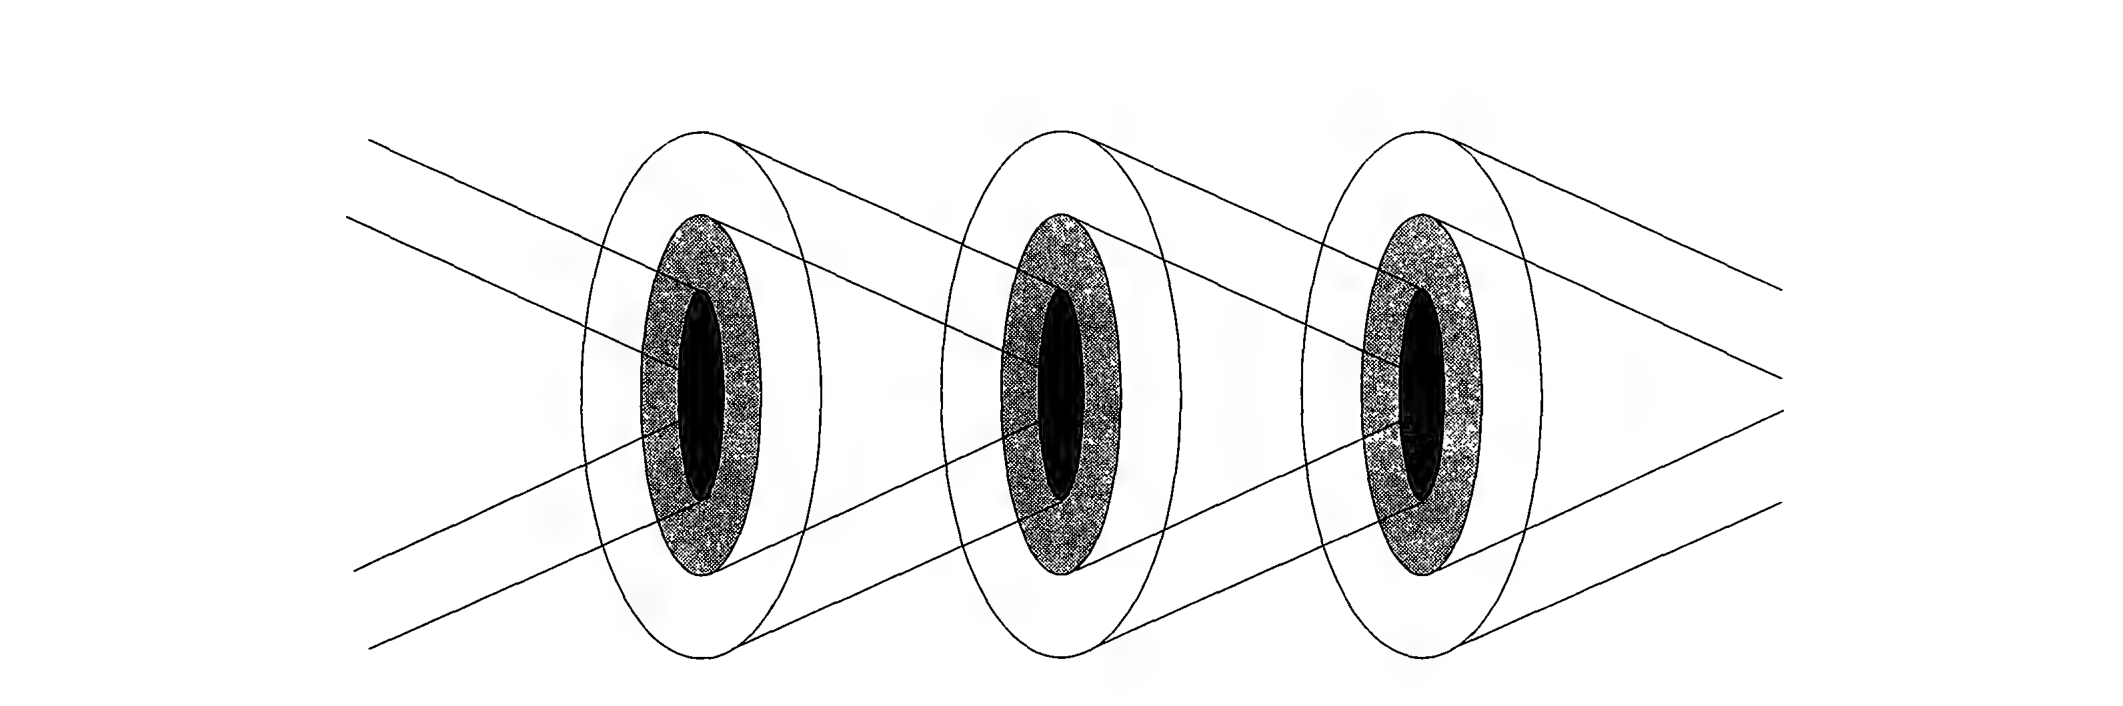
\includegraphics[width=0.88\textwidth]{figs/complex-heuristic.png}
\end{center}

椭圆是模 $M_i$; 黑色胖点是 $0$ 元素; 灰色椭圆在每一步被压扁到零, 它们是核; 由此我们形象地看到``前一个同态''的像落在``下一个同态''的核之内.

这幅图画并不精确之处在于: 它暗示 $d_{i+1}$ 的像与 $d_i$ 的核之间的``差'' (即着色较浅的灰色区域) 对所有的 $i$ 都相同; 当然一般情形并非如此. 事实上, 关于复形的几乎全部要点, 恰恰就是去``度量''这个差, 它被称为复形的同调%
\index{tongtiao@同调(homology)}
(参见 \S\ref{subsec:snake-lemma}). 若复形在``$M_i$ 处''没有同调, 我们就说它``在 $M_i$ 处''正合; 也就是说,
\[
\Image d_{i+1} = \Ker d_i.
\]
直观上看,
\begin{center}
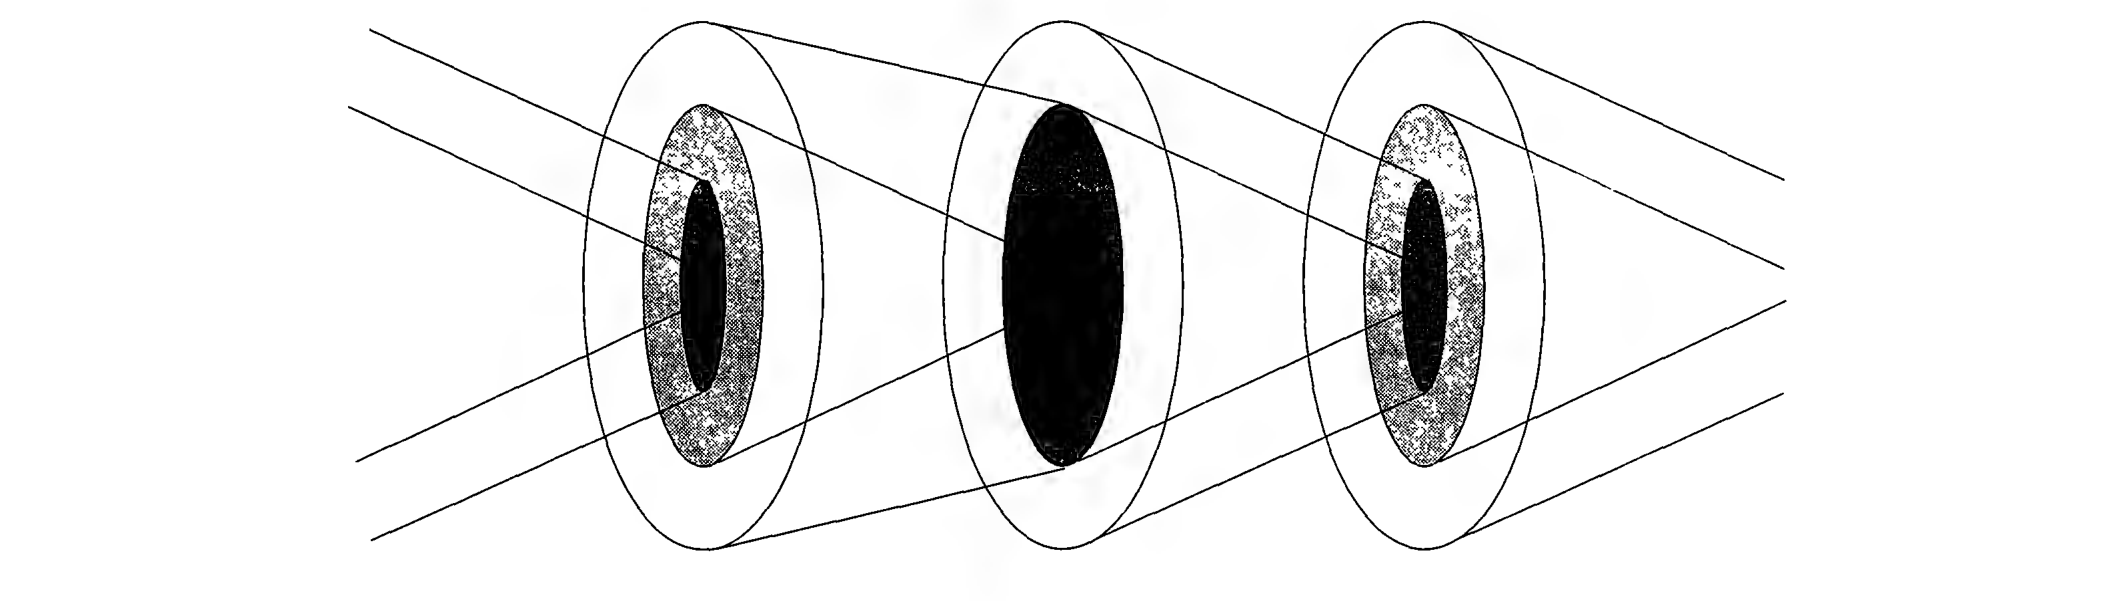
\includegraphics[width=0.88\textwidth]{figs/complex-exact.png}
\end{center}
这个复形看起来在中间那个椭圆处正合.

比如, 若 $M_i$ 是平凡模 (通常简单地记作 $0$), 则该复形必然在 $M_i$ 处正合, 因为此时 $\Image d_{i+1} = \Ker d_i = 0$.

若复形在它的所有模处都正合, 则称它是正合的, 并常被称为正合列%
\index{zhenghelie@正合列(exact sequence)}
.

\begin{example}
\label{ex:exact-mono}
复形
\[
\dots \longrightarrow 0 \longrightarrow L \xrightarrow{\ \alpha\ } M \longrightarrow \dots
\]
在 $L$ 处正合, 当且仅当 $\alpha$ 是单态射.

的确, 在 $L$ 处的正合等价于 $\Ker \alpha$ 等于平凡同态 $0 \to L$ 的像, 也就是说, 等价于
\[
\Ker \alpha = 0.
\]
这等价于 $\alpha$ 的单性 (命题~\ref{prop:mod-ker-coker}).
\end{example}

\begin{example}
\label{ex:exact-epi}
复形
\[
\dots \longrightarrow M \xrightarrow{\ \beta\ } N \longrightarrow 0 \longrightarrow \dots
\]
在 $N$ 处正合, 当且仅当 $\beta$ 是满态射.

的确, 该复形在 $N$ 处正合, 当且仅当 $\Image \beta$ 等于平凡同态 $N \to 0$ 的核, 也就是说, $\Image \beta = N$.
\end{example}

\begin{definition}
\label{def:short-exact}
短正合列%
\index{duanzhenghelie@短正合列(short exact sequence)}
是形如下式的正合复形:
\[
0 \longrightarrow L \xrightarrow{\ \alpha\ } M \xrightarrow{\ \beta\ } N \longrightarrow 0.
\]
\end{definition}

如前两例所见, 在 $L$ 与 $N$ 处的正合等价于 $\alpha$ 单、$\beta$ 满. 短正合列额外携带的信息是在 $M$ 处的正合, 也就是说,
\[
\Image \alpha = \Ker \beta;
\]
由第一同构定理 (推论~\ref{cor:module-first-iso}), 我们随之有
\[
N \cong \frac{M}{\Ker \beta} = \frac{M}{\Image \alpha}.
\]

总而言之, 我们手里有了进行更多巴甫洛夫式条件反射的好材料: 一看到上面那样的短正合列, 读者就应当本能地把 $L$ 认同为 $M$ 的子模 (经由单射 $\alpha$), 把 $N$ 认同为商 $M/L$ (经由满射 $\beta$ 在第一同构定理的庇护下诱导的同构).

短正合列在自然界中比比皆是. 比如, 单个同态 $\varphi : M \to M'$ 立即给出一个短正合列
\[
0 \longrightarrow \Ker \varphi \longrightarrow M \longrightarrow \Image \varphi \longrightarrow 0.
\]
事实上, 聚焦于短正合列的一个重要理由是: 这一观察使我们能够把每个正合复形打碎成大量的短正合列. 请欣赏这幅壮观的图:
\begin{center}
\begin{tikzcd}[column sep={4.4em,between origins}, row sep={2.3em,between origins}]
	&& 0 \ar[dr] && 0 && \\
	&&& \Image d_{i+1} = \Ker d_i \ar[ur] \ar[dr] &&& \\
	M_{i+2} \ar[rr, "d_{i+2}"] \ar[dr] && M_{i+1} \ar[rr, "d_{i+1}"] \ar[ur] && M_i \ar[rr, "d_i"] \ar[dr] && M_{i-1} \\
	& \Image d_{i+2} = \Ker d_{i+1} \ar[ur] \ar[dr] &&&& \Image d_i = \Ker d_{i-1} \ar[ur] \ar[dr] && \\
	0 \ar[ur] && 0 && 0 \ar[ur] && 0
\end{tikzcd}
\end{center}
斜向的序列是短正合列, 并且它们借助水平复形的正合性漂亮地互相咬合.

这一观察简化了许多论证; 参见例如习题~\ref{ex:noetherian-middle}.

\subsection{分裂正合列}
\label{subsec:split-exact}

短正合列的一种特殊情形, 来自考虑直和上的第二个投射: $M_1 \oplus M_2 \to M_2$; 于是有正合列
\[
0 \longrightarrow M_1 \longrightarrow M_1 \oplus M_2 \longrightarrow M_2 \longrightarrow 0,
\]
它通过把 $M_1$ 认同为该投射的核而得到. 这些短正合列被称为``分裂''的; 更一般地, 短正合列
\[
0 \longrightarrow M_1 \longrightarrow N \longrightarrow M_2 \longrightarrow 0
\]
称为``分裂''的, 如果它与上述序列之一同构, 意思是存在交换图
\begin{center}
\begin{tikzcd}
	0 \ar[r] & M_1 \ar[r] \ar[d, "\sim"'] & N \ar[r] \ar[d, "\sim"'] & M_2 \ar[r] \ar[d, "\sim"'] & 0 \\
	0 \ar[r] & M_1 \ar[r] & M_1 \oplus M_2 \ar[r] & M_2 \ar[r] & 0
\end{tikzcd}
\end{center}
其中竖直映射都是同构%
\footnote{事实上, 这最后一条要求有些多余; 参见习题~\ref{ex:extension-splits}.}%
.

\begin{example}
\label{ex:not-split}
$\Z$-模的正合列
\[
0 \longrightarrow \Z \xrightarrow{\ \cdot 2\ } \Z \longrightarrow \frac{\Z}{2\Z} \longrightarrow 0
\]
不分裂.
\end{example}

分裂序列给了我们一个机会, 回到 \S\ref{subsec:mod-ker-coker} 末尾悬而未决的问题: 对一个同态而言,``有左 (相应地, 右) 逆''这个条件应当怎么理解? 我们已经意识到这个条件比成为单态射\erratumfootnote{根据官方勘误, 原书英文此处将复数 monomorphisms 修正为单数 monomorphism.} (相应地, 满态射) 的要求更强; 我们能对这些态射给出更显式的描述吗?

\begin{proposition}
\label{prop:split-mono-epi}
设 $\varphi : M \to N$ 是 $R$-模同态. 那么
\begin{itemize}
	\item $\varphi$ 有左逆, 当且仅当序列
	\[
	0 \longrightarrow M \xrightarrow{\ \varphi\ } N \longrightarrow \Coker \varphi \longrightarrow 0
	\]
	分裂;
	\item $\varphi$ 有右逆, 当且仅当序列
	\[
	0 \longrightarrow \Ker \varphi \longrightarrow M \xrightarrow{\ \varphi\ } N \longrightarrow 0
	\]
	分裂.
\end{itemize}
\end{proposition}

\begin{proof}
我们证明第一部分, 另一部分作为练习留给读者 (习题~\ref{ex:split-epi}).

若序列分裂, 则可以把 $\varphi$ 认同为 $M$ 嵌入直和 $M \oplus M'$, 而投射 $M \oplus M' \to M$ 给出 $\varphi$ 的一个左逆. 反之, 设 $\varphi$ 有左逆 $\psi$:
\begin{center}
\begin{tikzcd}
	0 \ar[r] & M \ar[r,"\varphi"] \ar[dr,"\id_M"'] & N \ar[d,"\psi"] \\
& & M
\end{tikzcd}
\end{center}
那么我们断言: $N$ 同构于 $M \oplus \Ker \psi$, 且 $\varphi$ 对应于把 $M$ 认同第一因子: $M \to M \oplus \Ker \psi \cong N$. 同构 $M \oplus \Ker \psi \to N$ 由
\[
(m, k) \mapsto \varphi(m) + k
\]
给出; 它的逆 $N \to M \oplus \Ker \psi$ 是
\[
n \mapsto (\psi(n),\ n - \varphi\psi(n)).
\]
元素 $n - \varphi\psi(n)$ 在 $\Ker \psi$ 中, 理应如此, 因为
\[
\psi(n - \varphi\psi(n)) = \psi(n) - \psi\varphi\psi(n) = \psi(n) - \psi(n) = 0.
\]
所有必要的验证都是立即可得的, 留给读者.
\end{proof}

由于命题~\ref{prop:split-mono-epi}, 有左逆的 $R$-模同态称为分裂单态射%
\index{fenlidan@分裂单态射(split monomorphism)}
\index{fenlie@分裂(split)!yu@域(field)}, 有右逆的同态称为分裂满态射%
\index{fenliman@分裂满态射(split epimorphism)}
.

我们将在 \S IV.\ref{subsec:exact-sequences} (在要求更高的 $\cate{Grp}$ 语境中) 重回分裂正合列, 之后在我们回到模、以及更一般地回到 Abel 范畴 (第八与第九章) 时还会再遇到它们.

\subsection{同调与蛇形引理}
\label{subsec:snake-lemma}

\begin{definition}
\label{def:homology}
$R$-模的复形
\[
M_{\bullet}: \dots \xrightarrow{d_{i+2}} M_{i+1} \xrightarrow{d_{i+1}} M_i \xrightarrow{d_i} M_{i-1} \xrightarrow{d_{i-1}} \dots
\]
的第 $i$ 个同调是 $R$-模
\[
H_i(M_{\bullet}) := \frac{\Ker d_i}{\Image d_{i+1}}.
\]
\end{definition}

也就是说, $H_i(M_{\bullet})$ 是一个捕捉复形的启发式图像中``浅灰色环带''的模. 当然
\[
H_i(M_{\bullet}) = 0 \iff \Image d_{i+1} = \Ker d_i \iff \text{复形 } M_{\bullet} \text{ 在 } M_i \text{ 处正合}:
\]
也就是说, 同调模是``复形偏离正合的程度''的一种度量.

\begin{example}
\label{ex:homology-ker-coker}
事实上, 同调应当被想成核与余核这两个概念的 (宏伟的) 推广. 的确, 考虑 (非常) 特殊的情形: $M_{\bullet}$ 是复形
\[
0 \longrightarrow M_1 \xrightarrow{\ \varphi\ } M_0 \longrightarrow 0.
\]
那么
\[
H_1(M_{\bullet}) \cong \Ker \varphi, \qquad H_0(M_{\bullet}) \cong \Coker \varphi.
\]
\end{example}

我们将以指出一个涉及两个短正合列的交换图如何在同调中生成``长正合列''来结束这次对更抽象疆域的短暂访问. 这其实是更一般构造的特殊情形---按照那个构造, 一个涉及三个复形的适当交换图会产生一个真正长的``长正合同调列''. 当我们在第九章更深入地处理同调代数时, 会回到这个一般构造. 读者也很可能在代数拓扑的课程中学到它, 在那里这一事实被令人叹为观止地用于研究流形的不变量.

在我们要分析的简单形式中, 它被亲切地称为蛇形引理%
\index{shexingyinli@蛇形引理(snake lemma)}
. 考虑由同态相连的两个短正合列, 使它们构成交换图%
\footnote{事实上, 最好把这个图看作三个 (非常短的) 复形, 由 $R$-模同态 $\alpha_i$, $\beta_i$ 相连, 使得``行是正合的''. 其实, 人们可以定义复形的范畴, 而这个图不过是一个``复形的短正合列''; 这正是我们将在第九章采取的观点.}%
:
\begin{center}
\begin{tikzcd}[row sep=2.6em, column sep=2.6em]
	0 \ar[r] & L_1 \ar[r, "\alpha_1"] \ar[d, "\lambda"'] & M_1 \ar[r, "\beta_1"] \ar[d, "\mu"'] & N_1 \ar[r] \ar[d, "\nu"'] & 0 \\
	0 \ar[r] & L_0 \ar[r, "\alpha_0"'] & M_0 \ar[r, "\beta_0"'] & N_0 \ar[r] & 0
\end{tikzcd}
\end{center}

\begin{lemma}[蛇形引理]
\label{lem:snake}
沿用上图记号, 存在正合列
\[
0 \longrightarrow \Ker \lambda \longrightarrow \Ker \mu \longrightarrow \Ker \nu \xrightarrow{\ \delta\ } \Coker \lambda \longrightarrow \Coker \mu \longrightarrow \Coker \nu \longrightarrow 0.
\]
\end{lemma}

\begin{remark}
\label{rem:snake-induced}
该序列中的大多数同态都以完全直截了当的方式由相应的同态 $\lambda$, $\mu$, $\nu$ 诱导. 唯一``出人意料''的同态是记作 $\delta$ 的那一个; 我们将在下文讨论它的定义.
\end{remark}

\begin{remark}
\label{rem:snake-homology}
鉴于例~\ref{ex:homology-ker-coker}, 我们本可以把该陈述中的序列写成
\[
\begin{tikzcd}[column sep=1.4em,row sep=2.6em]
0 \ar[r] & H_1(L_\bullet) \ar[r] & H_1(M_\bullet) \ar[r] & H_1(N_\bullet) \ar[dlll,out=0,in=180,looseness=1.3,"\delta" description] \\
H_0(L_\bullet) \ar[r] & H_0(M_\bullet) \ar[r] & H_0(N_\bullet) \ar[r] & 0
\end{tikzcd}
\]
其中 $L_{\bullet}$ 是复形 $0 \longrightarrow L_1 \xrightarrow{\ \lambda\ } L_0 \longrightarrow 0$, 等等. 蛇形引理可以推广到任意复形 $L_{\bullet}$, $M_{\bullet}$, $N_{\bullet}$, 产生一个``长正合同调列'', 上式不过是它的尾端. 如上所述, 我们稍后会 (\S IX.\ref{subsec:3.3-les}) 讨论这个相当直截了当的推广.
\end{remark}

\begin{remark}
\label{rem:snake-general}
蛇形引理的一个流行版本不假定 $\alpha_1$ 单、$\beta_0$ 满: 也就是说, 我们可以考虑正合列的交换图
\begin{center}
\begin{tikzcd}[row sep=2.6em, column sep=2.6em]
	& L_1 \ar[r, "\alpha_1"] \ar[d, "\lambda"] & M_1 \ar[r, "\beta_1"] \ar[d, "\mu"] & N_1 \ar[r] \ar[d, "\nu"] & 0 \\
	0 \ar[r] & L_0 \ar[r, "\alpha_0"] & M_0 \ar[r, "\beta_0"] & N_0
\end{tikzcd}
\end{center}
此时引理将陈述: 存在``仅有的''正合列
\[
\Ker \lambda \longrightarrow \Ker \mu \longrightarrow \Ker \nu \xrightarrow{\ \delta\ } \Coker \lambda \longrightarrow \Coker \mu \longrightarrow \Coker \nu.
\]
\end{remark}

证明蛇形引理是一件不应当当众进行的事情, 而且把验证的细节写下来给别人看是出了名地无用: 那些细节本质上全都是显然的, 却会很快把人拖入记号的泥沼. 这类证明被统称为追图%
\index{zhuitu@追图(diagram chase)}
\index{gen@根(radical)!de@的(of)}的运动, 最佳的进行方式是: 在黑板上用几根手指同时指点图的不同部位, 一边念叨所摆弄的元素, 一边宣布它们的命运%
\footnote{真正的纯粹主义者会在任意范畴中追图, 从而没有谈论``元素''的便利; 我们稍后 (第九章) 会练习这项技能. 比如, 蛇形引理可以靠一个接一个地诉诸核与余核的万有性质来证明, 自始至终不选取任何元素. 但对着黑板指指点点、自言自语地过完论证的表演技巧, 本质上还是那一套.}%
.

尽管如此, 我们还是应当解释``连接''同态 $\delta$ 从何而来, 因为它是蛇形引理的陈述及其证明的核心. 这是包含核与余核的整幅图; 于是, 列是正合的 (连同水平放置的两条原序列也正合):
\begin{center}
\begin{tikzcd}[
row sep=1.2cm, column sep=1.2cm,
% 注意: execute at end picture 的大括号内绝对不能有“空行”, 否则会报 Runaway argument 错误！
execute at end picture={
\coordinate (p1) at ($(kg.east) + (2, 0)$);
\coordinate (mid) at ($(B.south)!0.55!(Bp.north)$);
\coordinate (p2) at (p1 |- mid);
\coordinate (p4) at ($(ca.west) - (2, 0)$);
\coordinate (p3) at (p4 |- p2);
\draw[->, rounded corners=12pt, thick, preaction={draw, white, line width=4pt}]
(kg.east) -- (p1) -- node[right] {$\delta$} (p2) -- (p3) -- (p4) -- (ca.west);
}
]
% 第 1 行
& 0 \arrow[d] & 0 \arrow[d] & 0 \arrow[d] & \\
% 第 2 行
0 \arrow[r] & \Ker\lambda \arrow[d] \arrow[r] & \Ker\mu \arrow[d] \arrow[r] & |[alias=kg]| \Ker\nu \arrow[d] & \\
% 第 3 行
0 \arrow[r] & L_1 \arrow[d, "\lambda" near start] \arrow[r, "\alpha_1"] & |[alias=B]| M_1 \arrow[d, "\mu" near start] \arrow[r, "\beta_1"] & N_1 \arrow[d, "\nu" near start] \arrow[r] & 0 \\
% 第 4 行
0 \arrow[r] & L_0 \arrow[d] \arrow[r, "\alpha_0"'] & |[alias=Bp]| M_0 \arrow[d] \arrow[r, "\beta_0"'] & N_0 \arrow[d] \arrow[r] & 0 \\
% 第 5 行
& |[alias=ca]| \Coker\lambda \arrow[d] \arrow[r] & \Coker\mu \arrow[d] \arrow[r] & \Coker\nu \arrow[d] \arrow[r] & 0 \\
% 第 6 行
& 0 & 0 & 0 &
\end{tikzcd}
\end{center}
顺便说, 我们相信读者现在明白了这条引理为何得名``蛇形''.

蛇形同态 $\delta$ 的定义. 设 $a \in \Ker \nu$. 我们断言: $a$ 可以沿着图中标记的实线箭头一路穿越到 $\Coker \lambda$:
\begin{center}
\begin{tikzcd}[row sep=1.6em,column sep=1.9em]
& 0 \ar[d,dotted,no head] & 0 \ar[d,dotted,no head] & 0 \ar[d,dotted,no head] & \\
0 \ar[r,dotted,no head] & \vphantom{e} \ar[r,dotted,no head] \ar[d,dotted,no head] & \vphantom{c} \ar[r,dotted,no head] \ar[d,dotted,no head] & a \ar[d] & \\
0 \ar[r,dotted,no head] & \vphantom{e} \ar[r,dotted,no head] \ar[d,dotted,no head] & c \ar[r,"\beta_1"] \ar[d,"\mu"] & b \ar[r,dotted,no head] \ar[d,dotted,no head,"\nu"] & 0 \\
0 \ar[r,dotted,no head] & e \ar[r,"\alpha_0"'] \ar[d] & d \ar[r,dotted,no head,"\beta_0"'] \ar[d,dotted,no head] & * \ar[r,dotted,no head] \ar[d,dotted,no head] & 0 \\
& f \ar[r,dotted,no head] \ar[d,dotted,no head] & \vphantom{f} \ar[r,dotted,no head] \ar[d,dotted,no head] & \vphantom{f} \ar[r,dotted,no head] \ar[d,dotted,no head] & 0 \\
& 0 & 0 & 0 &
\end{tikzcd}
\end{center}
的确,
\begin{itemize}
	\item $\Ker \nu \subseteq N_1$; 于是把 $a$ 视为 $N_1$ 的元素 $b$;
	\item $\beta_1$ 是满的, 故存在 $c \in M_1$ 映到 $b$;
	\item 令 $d = \mu(c)$ 为 $c$ 在 $M_0$ 中的像;
	\item $d$ 在标记 $*$ 的位置上的像是什么? 由图的交换性, 它必与 $\nu(b)$ 相同. 然而 $b$ 是 $a \in \Ker \nu$ 在 $N_1$ 中的像, 故 $\nu(b) = 0$. 于是 $d \in \Ker \beta_0$. 由于行正合, $\Ker \beta_0 = \Image \alpha_0$; 因此存在 $e \in L_0$ 映到 $d$;
	\item 最后, 令 $f \in \Coker \lambda$ 为 $e$ 的像.
\end{itemize}
我们想规定 $\delta(a) := f$.

这样做合法吗? 在追图的两步中我们取了原像:
\begin{itemize}
	\item 存在 $c \in M_1$ 使 $\beta_1(c) = b$;
	\item 存在 $e \in L_0$ 使 $\alpha_0(e) = d$.
\end{itemize}
第二步不涉及选择: 由于按假设 $\alpha_0$ 是单射, 映到 $d$ 的元素 $e$ 由 $d$ 唯一决定. 但第一步涉及选择: 为了验证 $\delta$ 是良定义的, 我们必须证明选取别的 $c$ 不会影响为 $\delta(a)$ 提议的值 $f$.

这要用另一次追图来证明. 图中相关的部分是:
\begin{center}
\begin{tikzcd}[row sep=2em,column sep=2em]
0 \ar[r,dotted,no head] & \vphantom{g} \ar[r,dotted,no head,"\alpha_1"] \ar[d,dotted,no head,"\lambda"'] & c \ar[r,"\beta_1"] \ar[d,"\mu"] & b \ar[r,dotted,no head] \ar[d,dotted,no head] & 0 \\
0 \ar[r,dotted,no head] & e \ar[r,"\alpha_0"'] \ar[d] & d \ar[r,dotted,no head] \ar[d,dotted,no head] & \vphantom{d} & \\
& f \ar[r,dotted,no head] & \vphantom{f} & &
\end{tikzcd}
\end{center}
假设我们选取映射到同一个 $b$ 的另一个 $c'$:
\[
\begin{tikzcd}
0 \ar[r,dotted,no head] & \vphantom{g} \ar[r,dotted,no head,"\alpha_1"] & c' \ar[r,"\beta_1"] & b \ar[r,dotted,no head] & 0
\end{tikzcd}.
\]
那么 $\beta_1(c' - c) = 0$; 由正合性, 存在 $g \in L_1$ 使 $(c' - c) = \alpha_1(g)$:
\[
g \xrightarrow{\ \alpha_1\ } (c' - c) \xrightarrow{\ \beta_1\ } 0.
\]
现在的要点是: 由于列构成复形, $g$ 在 $\Coker \lambda$ 中死去:
\[
\begin{tikzcd}[column sep=small]
0 \ar[r,dotted,no head] & g \ar[r,"\alpha_1"] \ar[d,"\lambda"'] & c'-c \ar[r,"\beta_1"] \ar[d,"\mu"] & 0 \\
0 \ar[r,dotted,no head] & \lambda(g) \ar[r,dotted,no head,"\alpha_0"] \ar[d] & \vphantom{d} \ar[r,dotted,no head] \ar[d,dotted,no head] & \vphantom{0} \\
& 0 \ar[r,dotted,no head] & \vphantom{f} &
\end{tikzcd}
\]
于是 (由图的交换性与 $\alpha_0$ 的单性) 得知: 把 $c$ 换成 $c'$ 会把 $e$ 修改为 $e + \lambda(g)$, 把 $f$ 修改为 $f + 0 = f$. 也就是说, $f$ 的确与选取无关.

于是 $\delta$ 是良定义的!

这只是蛇形引理证明的极小的一部分, 但大概足以说明为什么阅读写出来的追图过程可能极其缺乏信息量.

证明的其余部分 (留给读者 (!); 我们没有把它列为正式习题, 唯恐真有人交来一份作业等待评分) 由许许多多类似的论证组成. 在核与余核上诱导的映射的定义, 比上面描述的连接态射 $\delta$ 的定义要容易得多. 序列
\[
0 \longrightarrow \Ker \lambda \longrightarrow \Ker \mu \longrightarrow \Ker \nu \xrightarrow{\ \delta\ } \Coker \lambda \longrightarrow \Coker \mu \longrightarrow \Coker \nu \longrightarrow 0
\]
在大多数位置的正合性也相当直截了当; 大部分工作将花在证明在 $\Ker \nu$ 与 $\Coker \lambda$ 处的正合性上.

亲爱的读者: 不要回避尝试, 因为这是极好且不可或缺的练习. 错过这次机会, 你将永远对这类操作心中无底.

蛇形引理把若干个事实串成一线, 这些事实单独证明并不困难, 但引理一旦落定它们就变得真正直截了当. 比如,

\begin{corollary}
\label{cor:short-five}
在与蛇形引理相同的情形中 (记号同 \S\ref{subsec:snake-lemma}), 设 $\mu$ 是满的且 $\nu$ 是单的. 则 $\lambda$ 是满的, 且 $\nu$ 是同构.
\end{corollary}

\begin{proof}
的确, $\mu$ 满 $\implies \Coker \mu = 0$; $\nu$ 单 $\implies \Ker \nu = 0$ (命题~\ref{prop:mod-ker-coker}). 把这些信息输入蛇形引理的序列, 得到正合列
\[
0 \longrightarrow \Ker \lambda \longrightarrow \Ker \mu \longrightarrow 0 \longrightarrow \Coker \lambda \longrightarrow 0 \longrightarrow \Coker \nu \longrightarrow 0.
\]
正合性蕴含 $\Coker \lambda = \Coker \nu = 0$ (习题~\ref{ex:exact-zero}); 故 $\lambda$ 与 $\nu$ 是满的, 得到所述结论.
\end{proof}

还有几个这类陈述可以同样轻松地证明; 读者尽可随心所欲地试验.

\subsection*{习题}
\phantomsection
\addcontentsline{toc}{subsection}{习题}

\begin{prob}
\label{ex:exact-zero}
$\triangleright$ 设复形
\[
\dots \longrightarrow 0 \longrightarrow M \longrightarrow 0 \longrightarrow \dots
\]
正合. 证明 $M \cong 0$. [\S\ref{subsec:snake-lemma}]
\end{prob}

\begin{prob}
\label{ex:exact-iso}
设复形
\[
\dots \longrightarrow 0 \longrightarrow M \longrightarrow M' \longrightarrow 0 \longrightarrow \dots
\]
正合. 证明 $M \cong M'$.
\end{prob}

\begin{prob}
\label{ex:ker-coker-exact}
设复形
\[
\dots \longrightarrow 0 \longrightarrow L \longrightarrow M \xrightarrow{\ \varphi\ } M' \longrightarrow N \longrightarrow 0 \longrightarrow \dots
\]
正合. 证明: 在相差自然认同的意义下, $L = \Ker \varphi$ 且 $N = \Coker \varphi$.
\end{prob}

\begin{prob}
\label{ex:Hilbert-hotel}
构造 $\Z$-模的短正合列
\[
0 \longrightarrow \Z^{\oplus \N} \longrightarrow \Z^{\oplus \N} \longrightarrow \Z \longrightarrow 0
\]
与
\[
0 \longrightarrow \Z^{\oplus \N} \longrightarrow \Z^{\oplus \N} \longrightarrow \Z^{\oplus \N} \longrightarrow 0.
\]
(提示: David Hilbert 的大旅馆.)
\end{prob}

\begin{prob}
\label{ex:noetherian-middle}
$\triangleright$ 设复形
\[
\dots \longrightarrow L \longrightarrow M \longrightarrow N \longrightarrow \dots
\]
正合, 且 $L$ 与 $N$ 是 Noether 的. 证明 $M$ 是 Noether 的. [\S\ref{subsec:complexes}]
\end{prob}

\begin{prob}
\label{ex:split-epi}
$\triangleright$ 证明命题~\ref{prop:split-mono-epi} 的``分裂满态射''部分. [\S\ref{subsec:split-exact}]
\end{prob}

\begin{prob}
\label{ex:hom-left-exact}
$\triangleright$ 设
\[
0 \longrightarrow M \longrightarrow N \longrightarrow P \longrightarrow 0
\]
是 $R$-模的短正合列, $L$ 是 $R$-模.
\begin{itemize}
	\item[(i)] 证明存在正合列%
	\footnote{一般地, 这将是 Abel 群的序列; 若 $R$ 交换, 从而每个 $\Hom_{R\dcate{Mod}}$ 都是 $R$-模 (\S\ref{subsec:R-Mod-hom}), 则它将是 $R$-模的正合列.}
	\[
	0 \longrightarrow \Hom_{R\dcate{Mod}}(P, L) \longrightarrow \Hom_{R\dcate{Mod}}(N, L) \longrightarrow \Hom_{R\dcate{Mod}}(M, L).
	\]
	\item[(ii)] 重做习题~\ref{ex:hom-cyclic}. (用正合列 $0 \to I \to R \to R/I \to 0$.)
	\item[(iii)] 构造一个例子, 表明 (i) 中最右边的同态不必是满的.
	\item[(iv)] 证明: 若原序列分裂, 则 (i) 中最右边的同态是满的.
\end{itemize}
[\ref{ex:free-hom-exact}, VIII.\ref{ex:quotient-base-change}, \S~VIII.\ref{subsec:hom-adjunction-again}]
\end{prob}

\begin{prob}
\label{ex:free-splits}
$\triangleright$ 证明: $R$-模的每个正合列
\[
0 \longrightarrow M \longrightarrow N \longrightarrow F \longrightarrow 0,
\]
其中 $F$ 自由, 都分裂. (提示: 习题~\ref{ex:projective-free}.) [\S~VIII.\ref{subsec:duality-exactness}]
\end{prob}

\begin{prob}
\label{ex:free-hom-exact}
设
\[
0 \longrightarrow M \longrightarrow N \longrightarrow F \longrightarrow 0
\]
是 $R$-模的短正合列, $F$ 自由, $L$ 是 $R$-模. 证明存在正合列
\[
0 \longrightarrow \Hom_{R\dcate{Mod}}(F, L) \longrightarrow \Hom_{R\dcate{Mod}}(N, L) \longrightarrow \Hom_{R\dcate{Mod}}(M, L) \longrightarrow 0.
\]
(参见习题~\ref{ex:hom-left-exact}.)
\end{prob}

\begin{prob}
\label{ex:short-five}
\index{youxiankefenkuozhangshijiandande@有限可分扩张是简单的(finite separable extensions are simple)!wuyinli@五引理(five-lemma)!duan@短(short)}\index{youxiankefenkuozhangshijiandande@有限可分扩张是简单的(finite separable extensions are simple)!wuyinli@五引理(five-lemma)}$\triangleright$ 在蛇形引理的情形中, 设 $\lambda$ 与 $\nu$ 是同构. 用蛇形引理证明 $\mu$ 是同构. 它被称为``短五引理'', 因为它立即由五引理 (参见习题~\ref{ex:five-lemma}) 推出, 也由蛇形引理推出. [VIII.\ref{ex:ext-extensions}, IX.\ref{ex:2.4}]
\end{prob}

\begin{prob}
\label{ex:extension-splits}
$\triangleright$ 设
\begin{equation*}
0 \longrightarrow M_1 \longrightarrow N \longrightarrow M_2 \longrightarrow 0 \tag{$*$}
\end{equation*}
是 $R$-模的正合列. (它可以称为 $M_2$ 被 $M_1$ 扩张所得的一个``扩充''.) 设存在任意一个使图
\[
\begin{tikzcd}[column sep=small]
0 \ar[r] & M_1 \ar[r] \ar[d,equal] & N \ar[r] \ar[d,dashed] & M_2 \ar[r] \ar[d,equal] & 0 \\
0 \ar[r] & M_1 \ar[r] & M_1\oplus M_2 \ar[r] & M_2 \ar[r] & 0
\end{tikzcd}
\]
交换的 $R$-模同态 $N \to M_1 \oplus M_2$, 其中下方的序列是直和的标准序列. 证明 $(*)$ 分裂. [\S\ref{subsec:split-exact}]
\end{prob}

\begin{prob}
\index{siyinli@四引理(four-lemma)}\label{ex:four-lemma}
$\neg$ 用证明``四引理''来练习你的追图技艺: 若
\[
\begin{tikzcd}[column sep=small]
A_1 \ar[r] \ar[d, "\alpha"'] & B_1 \ar[r] \ar[d, "\beta"'] & C_1 \ar[r] \ar[d, "\gamma"'] & D_1 \ar[d, "\delta"'] \\
A_0 \ar[r] & B_0 \ar[r] & C_0 \ar[r] & D_0
\end{tikzcd}
\]
是行为正合的 $R$-模交换图, $\alpha$ 是满态射, $\beta$ 与 $\delta$ 是单态射, 则 $\gamma$ 是单态射. [\ref{ex:four-lemma-2}, IX.\ref{ex:2.3}]
\end{prob}

\begin{prob}
\label{ex:four-lemma-2}
证明习题~\ref{ex:four-lemma} 的``四引理''的另一个%
\footnote{事实上, 两个版本不必都证明; 但要意识到这一点, 必须从 Abel 范畴这一更一般的语境来看待问题; 参见习题~IX.\ref{ex:2.3}.}%
版本: 若
\[
\begin{tikzcd}[column sep=small]
B_1 \ar[r] \ar[d, "\beta"'] & C_1 \ar[r] \ar[d, "\gamma"'] & D_1 \ar[r] \ar[d, "\delta"'] & E_1 \ar[d, "\epsilon"'] \\
B_0 \ar[r] & C_0 \ar[r] & D_0 \ar[r] & E_0
\end{tikzcd}
\]
是行为正合的 $R$-模交换图, $\beta$ 与 $\delta$ 是满态射, $\epsilon$ 是单态射, 则 $\gamma$ 是满态射.
\end{prob}

\begin{prob}
\label{ex:five-lemma}
$\neg$ 证明``五引理'': 若
\begin{center}
\begin{tikzcd}[row sep=2.2em, column sep=1.9em]
	A_1 \ar[r] \ar[d, "\alpha"'] & B_1 \ar[r] \ar[d, "\beta"'] & C_1 \ar[r] \ar[d, "\gamma"'] & D_1 \ar[r] \ar[d, "\delta"'] & E_1 \ar[d, "\epsilon"'] \\
	A_0 \ar[r] & B_0 \ar[r] & C_0 \ar[r] & D_0 \ar[r] & E_0
\end{tikzcd}
\end{center}
是行为正合的 $R$-模交换图, $\beta$ 与 $\delta$ 是同构, $\alpha$ 是满态射, $\epsilon$ 是单态射, 则 $\gamma$ 是同构. (把前面几道习题的结果拼接起来, 可以避免所需的追图.) [\ref{ex:short-five}]
\end{prob}

\begin{prob}
\index{jiuyinli@九引理(nine-lemma)}\label{ex:nine-lemma}
$\neg$ 考虑下面的 $R$-模交换图:
\begin{center}
\begin{tikzcd}[row sep=1.8em,column sep=1.9em]
&0 \ar[d] &0 \ar[d] &0 \ar[d] & \\
0 \ar[r] &L_2 \ar[r] \ar[d] &M_2 \ar[r] \ar[d,"\alpha"] &N_2 \ar[r] \ar[d] &0 \\
0 \ar[r] &L_1 \ar[r] \ar[d] &M_1 \ar[r] \ar[d,"\beta"] &N_1 \ar[r] \ar[d] &0 \\
0 \ar[r] &L_0 \ar[r] \ar[d] &M_0 \ar[r] \ar[d] &N_0 \ar[r] \ar[d] &0 \\
&0 &0 &0 &
\end{tikzcd}
\end{center}
设三行都正合, 且最右边的两列正合. 证明左列正合. 第二版本: 设三行都正合, 且最左边的两列正合; 证明右列正合. 这就是``九引理''. (对图作 $90^{\circ}$ 旋转后应用蛇形引理, 可以避免追图.) [\ref{ex:nine-lemma-2}]
\end{prob}

\begin{prob}
\label{ex:nine-lemma-2}
在与习题~\ref{ex:nine-lemma} 相同的情形中, 设三行都正合, 且最左列与最右列正合.
\begin{itemize}
	\item 证明 $\alpha$ 是单态射, $\beta$ 是满态射.
	\item 中间列必然正合吗?
\end{itemize}
(提示: 不必然. 把 $\Z \oplus \Z$ 放在中间, 并用六份 $\Z$ 与两个 $0$ 巧妙地围住它.)
再假定中央列是复形, 即 $\beta\circ\alpha=0$; 证明此时中央列必正合.
\end{prob}

\begin{prob}
\label{ex:infinite-nine-lemma}
$\neg$ 如下推广前两道习题. 考虑一个 (可能无限的) $R$-模交换图:
\[
\begin{tikzcd}[row sep=1.8em,column sep=2em]
&\vdots \ar[d] &\vdots \ar[d] &\vdots \ar[d] & \\
0 \ar[r] &L_{i+1} \ar[r] \ar[d] &M_{i+1} \ar[r] \ar[d] &N_{i+1} \ar[r] \ar[d] &0 \\
0 \ar[r] &L_i \ar[r] \ar[d] &M_i \ar[r] \ar[d] &N_i \ar[r] \ar[d] &0 \\
0 \ar[r] &L_{i-1} \ar[r] \ar[d] &M_{i-1} \ar[r] \ar[d] &N_{i-1} \ar[r] \ar[d] &0 \\
&\vdots &\vdots &\vdots &
\end{tikzcd}
\]
其中中央列是复形, 且每行都正合. 证明左列与右列也是复形. 证明任意两列正合时, 第三列也正合. (第一部分是直截了当的. 第二部分由于需要追图, 现在会花你几分钟; 等学过 \S~IX.\ref{subsec:3.3-les} 的长正合 (上) 同调列之后, 只需几秒钟.) [IX.\ref{ex:3.12}]
\end{prob}

% 第四章 群: 再次相遇 --- 中译
% 原书 pp. 171--236 (Aluffi, Algebra: Chapter 0, Chapter IV).
% 本文件进度: §\ref{sec:conjugation}--§\ref{subsec:sylow} 已译 (2026-08-29); §\ref{sec:composition-solvability} 以下待续.

\chapter{群:再次相遇}
\label{chap:groups2}

在本章中, 我们回到 $\cate{Grp}$, 研究若干比第二章所考虑的内容``更不一般''的课题. 我们在这里所做的大部分内容将专门适用于有限群; 这本身就是一个重要的例子, 因为它有着辉煌的应用 (例如在 Galois 理论中; 参见 \S VII.\ref{sec:galois-applications}), 而且从叙述的角度看它也是一个好题材, 因为它使我们有机会看到几个一般概念在一个足够复杂以承载实质内容、又足够简单以易于领会 (就这一小撮初等课题而言) 的语境中发挥作用.

\section{共轭作用}
\label{sec:conjugation}

\subsection{群在集合上的作用: 回顾}
\label{subsec:actions-reminder}

当你让群作用在什么东西上时, 群才真正大放异彩. 本节将非常有效地证明这一点, 因为通过对 \S~II.\ref{subsec:transitive-actions} 中建立的关于群作用的初等事实进行极其头脑简单的应用, 我们将得到关于有限群的出奇精确的结果.

回顾我们证明过 (命题~II.\ref{prop:transitive-orbits}): 群 $G$ 在集合 $S$ 上的每个传递的 (左) 作用, 在相差自然同构概念的意义下, 都是``在左陪集之集 $G/H$ 上的左乘''. 这里 $H$ 可以取为任意元素 $a \in S$ 的稳定子 $\Stab_G(a)$, 即 (定义~II.\ref{def:stabilizer}) 固定 $a$ 的 $G$ 的子群. 这一事实适用于 $G$ 在一个集合上的每个左作用的轨道; 特别地, 有限轨道 $O$ 中元素的个数等于 $O$ 中任意 $a$ 的稳定子的指数; 特别地 (推论~II.\ref{cor:orbit-divides}), 若 $G$ 有限, 则轨道的元素个数 $|O|$ 必须整除 $G$ 的阶 $|G|$.

这些考虑可以打包成一个有用的``计数''公式, 对那个作用我们可以称之为类公式%
\index{leigongshi@类公式(class formula)}
; 这个名字通常保留给 $G$ 通过共轭作用于自身的特殊情形, 我们将在下文更仔细地探讨它.

为陈述该公式, 设 $G$ 作用在集合 $S$ 上; 对 $a \in S$, 令 $G_a$ 表示稳定子 $\Stab_G(a)$. 再令 $Z$ 为作用的不动点之集:
\[
Z = \{a \in S \mid (\forall g \in G):\ ga = a\}.
\]
注意 $a \in Z \iff G_a = G$; 我们可以说, $a \in Z$ 当且仅当 $a$ 的轨道是``平凡的'', 意思是它仅由 $a$ 一人组成.

\begin{proposition}
\label{prop:class-formula}
设 $S$ 是有限集, $G$ 是作用在 $S$ 上的群. 沿用上面的记号,
\[
|S| = |Z| + \sum_{a \in A} [G:G_a],
\]
其中 $A \subseteq S$ 对该作用的每个非平凡轨道恰含一个元素.
\end{proposition}

\begin{proof}
轨道构成 $S$ 的一个划分, 而 $Z$ 收集了平凡的轨道; 于是
\[
|S| = |Z| + \sum_{a \in A} |O_a|,
\]
其中 $O_a$ 表示 $a$ 的轨道. 由命题~II.\ref{prop:transitive-orbits}, 阶 $|O_a|$ 等于 $a$ 的稳定子的指数, 即得所述.
\end{proof}

命题~\ref{prop:class-formula} 的主要力量在于: 若 $G$ 有限, 则每个和项 $[G:G_a]$ 整除 $G$ 的阶 (且大于 $1$). 当关于 $|G|$ 的某些信息已知时, 这可以是一个很强的约束. 比如, 看看当 $G$ 是 $p$-群时它说了什么:

\begin{definition}
\label{def:p-group}
$p$-群%
\index{pqun@p-群(p-group)}
是阶为素整数 $p$ 的幂的有限群.
\end{definition}

\begin{corollary}
\label{cor:fixed-points}
设 $G$ 是作用在有限集 $S$ 上的 $p$-群, $Z$ 是该作用的不动点之集. 则
\[
|Z| \equiv |S| \bmod p.
\]
\end{corollary}

\begin{proof}
的确, 命题~\ref{prop:class-formula} 中的每个和项 $[G:G_a]$ 都是大于 $1$ 的 $p$ 的幂; 从而它模 $p$ 为 $0$.
\end{proof}

例如, 在某些情形这可以用来确立 $Z \neq \emptyset$%
\footnote{在这个意义下, 命题~\ref{prop:class-formula} 是一类被称为``不动点定理''的结果的一个实例. 读者在拓扑学课程中多半会遇到几个这样的定理, 在那里集合的``大小''的角色可以 (比如) 由拓扑空间的 Euler 示性数来扮演.}%
: 见习题~\ref{ex:p-group-fixed}. 命题~\ref{prop:class-formula} 的这类直接推论将在下文西罗定理的证明中助我们一臂之力.

\index{gongelei@共轭类(conjugacy class)!zai $S_n$ zhong@在 $S_n$ 中(in $S_n$)}\subsection{中心、中心化子、共轭类}
\label{subsec:center-conjugacy}

回顾 (例~II.\ref{ex:left-multiplication}) 每个群 $G$ 都以至少两种有趣的方式作用于自身: 通过 (左) 乘与通过共轭%
\index{gonge@共轭(conjugation)}
. 后一作用由如下 $\rho : G \times G \to G$ 定义:
\[
\rho(g, a) = gag^{-1}.
\]
如我们所知 (\S~II.\ref{subsec:actions-sets}), 这一数据等价于某个群同态的数据:
\[
\sigma : G \to S_G,
\]
即从 $G$ 到 $G$ 上的置换群的群同态.

这个作用凸显了几个有趣的对象:

\begin{definition}
\label{def:center}
$G$ 的中心%
\index{zhongxin@中心(center)}
, 记作 $Z(G)$, 是 $G$ 的子群 $\Ker \sigma$.
\end{definition}

具体地说, $G$ 的中心\footnote{为何用 $Z$? ``中心''的德文是 Zentrum.}是
\[
Z(G) = \{g \in G \mid (\forall a \in G):\ ga = ag\}.
\]
的确, $\sigma(g)$ 是 $S_G$ 中的恒同, 当且仅当 $\sigma(g)$ 在 $G$ 上作为恒同作用; 也就是说, 当且仅当对所有 $a \in G$ 有 $gag^{-1} = a$; 也就是说, 当且仅当 $g$ 与 $G$ 的所有元素交换. 换言之, 中心是 $G$ 在共轭作用下的不动点之集.

注意, 群 $G$ 的中心自动在 $G$ 中正规: ``手工''验证这几乎是立即的, 但无需这么做, 因为按定义它是一个核, 而核是正规的.

群 $G$ 交换, 当且仅当 $Z(G) = G$, 也就是说, 当且仅当共轭作用在 $G$ 上是平凡的.

\index{guina@归纳(induction)}一般地, 当你发现一个群的中心非平凡时, 尽管高兴: 这常常使你能对群的元素个数作归纳来建立证明, 办法是模掉中心 (大致说来, 这正是我们将证明第一西罗定理的方式). 或者注意下面这个在试图证明群交换时很顺手的有用事实:

\begin{lemma}
\label{lem:quotient-center-cyclic}
设 $G$ 是有限群, 且 $G/Z(G)$ 是循环的. 则 $G$ 是交换的 (从而 $G/Z(G)$ 事实上是平凡的).
\end{lemma}

\begin{proof}
(参见习题~\ref{ex:G-Z-cyclic-inn}.) 由于 $G/Z(G)$ 循环, 存在元素 $g \in G$ 使得类 $gZ(G)$ 生成 $G/Z(G)$. 那么 $\forall a \in G$
\[
aZ(G) = (gZ(G))^r
\]
对某个 $r \in \Z$ 成立; 也就是说, 存在中心的元素 $z \in Z(G)$ 使 $a = g^r z$.

现在若 $a$, $b$ 属于 $G$, 利用这一事实写
\[
a = g^r z, \qquad b = g^s w
\]
对某个 $s \in \Z$ 与 $w \in Z(G)$ 成立; 然而
\[
ab = (g^r z)(g^s w) = g^{r+s}zw = (g^s w)(g^r z) = ba,
\]
其中我们用到了 $z$ 与 $w$ 同 $G$ 的每个元素交换这一事实. 由于 $a$ 与 $b$ 是任意的, 这证明 $G$ 交换.
\end{proof}

接下来, $a \in G$ 在共轭下的稳定子有一个特别的名字:

\begin{definition}
\label{def:centralizer}
$a \in G$ 的中心化子%
\index{zhongxinhazi@中心化子(centralizer)}
(或正规化子%
\index{zhengguihuazi@正规化子(normalizer)}
) $Z_G(a)$ 是它在共轭下的稳定子.
\end{definition}

于是,
\[
Z_G(a) = \{g \in G \mid gag^{-1} = a\} = \{g \in G \mid ga = ag\}
\]
由 $G$ 中那些与 $a$ 交换的元素构成. 特别地, 对所有 $a \in G$ 有 $Z(G) \subseteq Z_G(a)$; 事实上, $Z(G) = \bigcap_{a \in G} Z_G(a)$. 显然 $a \in Z(G) \iff Z_G(a) = G$.

若对包含 $a$ 的群 $G$ 不存在歧义, 则可省去下标 $G$.

\begin{definition}
\label{def:conjugacy-class}
$a \in G$ 的共轭类%
\index{gonggelei@共轭类(conjugacy class)}
是 $a$ 在共轭作用下的轨道 $[a]$. $G$ 的两个元素 $a$, $b$ 称为共轭的%
\index{gonggede@共轭的(conjugate)}
, 如果它们属于同一个共轭类.
\end{definition}

记号 $[a]$ 并不标准; $C(a)$ 使用得更频繁, 但我们不喜欢它. 使用 $[a]$ 提醒我们: 这些不过是 $G$ 的元素在某个有趣的等价关系之下的等价类.

注意 $[a] = \{a\}$ 当且仅当对所有 $g \in G$ 有 $gag^{-1} = a$; 也就是说, 当且仅当对所有 $g \in G$ 有 $ga = ag$; 也就是说, 当且仅当 $a \in Z(G)$.

\subsection{类公式}
\label{subsec:class-formula}

有限群 $G$ 的``正式''类公式, 是命题~\ref{prop:class-formula} 用于共轭作用的特殊情形.

\begin{proposition}[类公式]
\label{prop:class-formula-conj}
设 $G$ 是有限群. 则
\[
|G| = |Z(G)| + \sum_{a \in A} [G:Z(a)],
\]
其中 $A \subseteq G$ 是为 $G$ 中每个非平凡共轭类取一个代表元的集合.
\end{proposition}

\begin{proof}
不动点之集是 $Z(G)$, 而 $a$ 的稳定子是中心化子 $Z(a)$; 应用命题~\ref{prop:class-formula}.
\end{proof}

类公式出奇地有用. 在应用它时, 记住右边的每一项 (即 $|Z(G)|$ 与每个 $[G:Z(a)]$) 都整除 $|G|$; 仅此一条常常就足以对 $G$ 引人注目的结论.

也许最著名的这类应用是通过推论~\ref{cor:fixed-points} 用于 $p$-群:

\begin{corollary}
\label{cor:p-group-center}
设 $G$ 是非平凡的 $p$-群. 则 $G$ 有非平凡的中心.
\end{corollary}

\begin{proof}
由于 $|Z(G)| \equiv |G| \bmod p$ 且 $|G| > 1$ 是 $p$ 的幂, $|Z(G)|$ 必是 $p$ 的倍数. 由于 $Z(G) \neq \emptyset$ (因为 $e_G \in Z(G)$), 这蕴含 $|Z(G)| \geq p$.
\end{proof}

比如, (由推论~\ref{cor:p-group-center} 与引理~\ref{lem:quotient-center-cyclic}; 参见习题~\ref{ex:pq-center}) 立即得到: 若 $p$ 是素数, 则每个 $p^2$ 阶群都是交换的.

一般地, 类公式对一个群中可能发生的事情施加强约束.

\begin{example}
\label{ex:order-6}
考虑一个 $6$ 阶群 $G$; 它的类公式有哪些可能?

若 $G$ 交换, 则类公式告诉我们很少:
\[
6 = 6.
\]
若 $G$ 不交换, 则它的中心必是平凡的 (由 Lagrange 定理与引理~\ref{lem:quotient-center-cyclic} 推出); 于是类公式是 $6 = 1 + \cdots$, 其中 $\cdots$ 收集诸非平凡共轭类的大小. 但这些和项中的每一个都必须大于 $1$、小于 $6$, 且必须整除 $6$; 也就是说, 别无选择:
\[
6 = 1 + 2 + 3
\]
是唯一的可能. 读者应当验证这的确是 $S_3$ 的类公式; 事实上, 在相差同构的意义下, $S_3$ 是唯一的 $6$ 阶非交换群 (习题~\ref{ex:order-6-S3}).
\end{example}

另一个有用的观察是: 正规子群必须是共轭类的并: 因为若 $H$ 是正规子群, $a \in H$, 且 $b = gag^{-1}$ 与 $a$ 共轭, 那么
\[
b \in gHg^{-1} = H.
\]

仍以 $|G| = 6$ 的例子为念, 注意群的每个子群必含恒同元, 且其大小必整除群的阶; 由此可知: $6$ 阶非交换群的正规子群不可能有阶 $2$, 因为 $2$ 无法写成共轭类之阶的和 (包括恒同元所在的类).

\subsection{子集与子群的共轭}
\label{subsec:conjugation-subsets}

我们还可以通过共轭作用在 $G$ 的幂集上: 若 $A \subseteq G$ 是子集, $g \in G$, 则 $A$ 的共轭是子集 $gAg^{-1}$. 由消去律, 共轭映射 $a \mapsto gag^{-1}$ 是 $A$ 与 $gAg^{-1}$ 之间的双射.

这引出与 \S\ref{subsec:center-conjugacy} 中所引入的类似的术语.

\begin{definition}
\label{def:normalizer}
$A$ 的正规化子 $N_G(A)$ 是它在共轭下的稳定子. $A$ 的中心化子是固定 $A$ 的每个元素的子群 $Z_G(A) \subseteq N_G(A)$.
\end{definition}

于是, $g \in N_G(A)$ 当且仅当 $gAg^{-1} = A$%
\footnote{若 $A$ 有限 (但一般情形不然), 这一条件等价于 $gAg^{-1} \subseteq A$.}%
, 而 $g \in Z_G(A)$ 当且仅当 $\forall a \in A$, $gag^{-1} = a$.

对 $A = \{a\}$ 为单元素集的情形, 我们有 $N_G(\{a\}) = Z_G(\{a\}) = Z_G(a)$. 一般地, $Z_G(A) \subsetneq N_G(A)$.

若 $H$ 是 $G$ 的子群, 则 $H$ 的每个共轭 $gHg^{-1}$ 也是 $G$ 的子群; 共轭的子群有相同的阶.

\begin{remark}
\label{rem:normalizer}
该定义立即蕴含 $H \subseteq N_G(H)$, 并且 $H$ 在 $G$ 中正规, 当且仅当 $N_G(H) = G$. 更一般地, $H$ 在 $G$ 中的正规化子 $N_G(H)$ (显然) 是 $G$ 的使 $H$ 正规的最大子群.
\end{remark}

人们可以把命题~\ref{prop:class-formula} 应用于子集或子群上的共轭作用; 然而, 子集实在太多, 而人们对子群的个数又缺乏控制. 涉及给定子集或子群的共轭个数的其他数值考量可能非常有用\erratumfootnote{根据官方勘误, 原书此处明确将共轭作用的对象补充为子集或子群 (subgroups).}.

\begin{lemma}
\label{lem:number-of-conjugates}
设 $H \subseteq G$ 是子群. 那么 (若有限) 与 $H$ 共轭的子群的个数等于 $H$ 的正规化子在 $G$ 中的指数 $[G:N_G(H)]$.
\end{lemma}

\begin{proof}
这又是命题~II.\ref{prop:transitive-orbits} 的直接推论.
\end{proof}

\begin{corollary}
\label{cor:conjugates-divide}
若 $[G:H]$ 有限, 则与 $H$ 共轭的子群的个数有限, 且整除 $[G:H]$.
\end{corollary}

\begin{proof}
\[
[G:H] = [G:N_G(H)] \cdot [N_G(H):H]
\]
(参见 \S~II.\ref{subsec:index-lagrange}).
\end{proof}

著名的西罗定理之一, 将在 $H$ 是有限群 $G$ 中极大 $p$-群的情形下实质性地强化这一陈述. 关于群的任意 $p$-子群的正规化子之大小的陈述, 见引理~\ref{lem:normalizer-congruence}.

另一个有用的数值工具是如下观察: 若 $H$ 与 $K$ 是群 $G$ 的子群且 $H \subseteq N_G(K)$---从而对所有 $g \in H$ 有 $gKg^{-1} = K$---则用 $g \in H$ 作共轭给出 $K$ 的一个自同构. 的确, 我们已经观察到共轭是双射, 且容易看出它是同态: $\forall k_1, k_2 \in K$
\[
(gk_1g^{-1})(gk_2g^{-1}) = gk_1(g^{-1}g)k_2g^{-1} = g(k_1k_2)g^{-1}.
\]
于是, 共轭给出一个集合映射
\[
\gamma : H \to \Aut_{\cate{Grp}}(K).
\]
读者将验证这是一个群同态, 并将确定 $\Ker \gamma$ (习题~\ref{ex:gamma-hom}).

若 $H$ 有限, 且我们知道 $\Aut_{\cate{Grp}}(K)$ 的一些信息, 这一点特别有用 (例如, 参见习题~\ref{ex:center-an}). 习题~\ref{ex:cyclic-normal-central} 给出了一个经典应用.

\subsection*{习题}
\phantomsection
\addcontentsline{toc}{subsection}{习题}

\begin{prob}
\label{ex:p-group-fixed}
$\triangleright$ 设 $p$ 是素整数, $G$ 是 $p$-群, $S$ 是满足 $|S| \not\equiv 0 \bmod p$ 的集合. 若 $G$ 作用在 $S$ 上, 证明该作用必有不动点. [\S\ref{subsec:actions-reminder}, \S\ref{subsec:sylow-I}]
\end{prob}

\begin{prob}
\label{ex:center-dihedral}
求 $D_{2n}$ 的中心. (答案依赖于 $n$ 的奇偶性. 你已在习题~II.\ref{ex:order-gh-n} 中做过这道题; 这次使用一个表现.)
\end{prob}

\begin{prob}
\label{ex:center-sn}
证明当 $n \geq 3$ 时 $S_n$ 的中心是平凡的. (设 $\sigma \in S_n$ 把 $a$ 送到 $b \neq a$, 并设 $c \neq a, b$. 令 $\tau$ 为仅交换 $b$ 与 $c$ 的置换. 然后比较 $\sigma\tau$ 与 $\tau\sigma$ 在 $a$ 上的作用.)
\end{prob}

\begin{prob}
\label{ex:center-subgroup-normal}
$\triangleright$ 设 $G$ 是群, $N$ 是 $Z(G)$ 的子群. 证明 $N$ 在 $G$ 中正规. [\S\ref{subsec:sylow-I}]
\end{prob}

\begin{prob}
\label{ex:G-Z-cyclic-inn}
$\triangleright$ 设 $G$ 是群. 证明 $G/Z(G)$ 同构于 $G$ 的内自同构群 $\Inn(G)$. (参见习题~II.\ref{ex:inner-automorphisms}.) 然后利用习题~II.\ref{ex:inn-subgroup} 的结果把引理~\ref{lem:quotient-center-cyclic} 再证一遍. [\S\ref{subsec:center-conjugacy}]
\end{prob}

\begin{prob}
\label{ex:pq-center}
$\triangleright$ 设 $p$, $q$ 是素整数, $G$ 是 $pq$ 阶群. 证明要么 $G$ 交换, 要么 $G$ 的中心平凡. 由此断言 (用推论~\ref{cor:p-group-center}): 对素数 $p$, 每个 $p^2$ 阶群都交换. [\S\ref{subsec:class-formula}]
\end{prob}

\begin{prob}
\label{ex:p3-commutative}
证明或否证: 若 $p$ 是素数, 则每个 $p^3$ 阶群都交换.
\end{prob}

\begin{prob}
\label{ex:p-subgroup-chain}
$\triangleright$ 设 $p$ 是素数, $G$ 是 $p$-群: $|G| = p^r$. 证明对每个非负整数 $k \leq r$, $G$ 含有 $p^k$ 阶的正规子群. [\S\ref{subsec:sylow-I}]
\end{prob}

\begin{prob}
\label{ex:normal-intersects-center}
$\neg$ 设 $p$ 是素数, $G$ 是 $p$-群, $H$ 是 $G$ 的非平凡正规子群. 证明 $H \cap Z(G) \neq \{e\}$. (提示: 用类公式.) [\ref{ex:nilpotent-intersect-center}]
\end{prob}

\begin{prob}
\label{ex:odd-conjugate}
证明: 若 $G$ 是奇数阶群且 $g \in G$ 与 $g^{-1}$ 共轭, 则 $g = e_G$.
\end{prob}

\begin{prob}
\label{ex:commuting-representatives}
设 $G$ 是有限群, 并设 $g_1,\ldots,g_r$ 是 $G$ 的全部 $r$ 个共轭类的代表元, 使得 $\forall i, j$, $g_ig_j = g_jg_i$. 证明 $G$ 交换. (提示: 关于共轭类的大小你能说些什么?)
\end{prob}

\begin{prob}
\label{ex:class-formula-d8-q8}
验证 $D_8$ 与 $Q_8$ (参见习题~III.\ref{ex:quaternions}) 的类公式都是 $8 = 2 + 2 + 2 + 2$. (另注意 $D_8 \not\cong Q_8$.)
\end{prob}

\begin{prob}
\label{ex:order-6-S3}
$\triangleright$ 设 $G$ 是 $6$ 阶非交换群. 如例~\ref{ex:order-6} 中所观察, $G$ 必有平凡中心, 且恰有两个共轭类, 阶分别为 $2$ 与 $3$.
\begin{itemize}
	\item 证明: 若群的每个元素的阶都 $\leq 2$, 则该群交换. 由此断言 $G$ 有一个 $3$ 阶元素 $y$.
	\item 证明 $\langle y \rangle$ 在 $G$ 中正规.
	\item 证明 $[y]$ 是阶为 $2$ 的共轭类, 且 $[y] = \{y, y^2\}$.
	\item 证明存在 $x \in G$ 使 $yx = xy^2$.
	\item 证明 $x$ 有阶 $2$.
	\item 证明 $x$ 与 $y$ 生成 $G$.
	\item 证明 $G \cong S_3$.
\end{itemize}
[\S\ref{subsec:class-formula}, \S\ref{subsec:pq-groups}]
\end{prob}

\begin{prob}
\label{ex:conjugates-bound}
设 $G$ 是群, 且 $[G:Z(G)] = n$ 有限. 设 $A \subseteq G$ 是任意子集. 证明 $A$ 的共轭至多 $n$ 个.
\end{prob}

\begin{prob}
\label{ex:class-formula-60}
设群 $G$ 的类公式为 $60 = 1 + 15 + 20 + 12 + 12$. 证明 $G$ 的仅有的正规子群是 $\{e\}$ 与 $G$.
\end{prob}

\begin{prob}
\label{ex:index-2-classes}
$\triangleright$ 设 $G$ 是有限群, $H \subseteq G$ 是指数为 $2$ 的子群. 对 $a \in H$, 用 $[a]_H$ (相应地, $[a]_G$) 记 $a$ 在 $H$ 中 (相应地, 在 $G$ 中) 的共轭类. 证明: 按照中心化子 $Z_G(a)$ 不含于还是含于 $H$, $[a]_H = [a]_G$ 或 $[a]_H$ 是 $[a]_G$ 的一半大小. (提示: 注意由习题~II.\ref{ex:index-2-normal}, $H$ 在 $G$ 中正规; 应用命题~II.\ref{prop:second-iso}.) [\S\ref{subsec:symmetric-group-type}]
\end{prob}

\begin{prob}
\label{ex:union-of-conjugates}
$\neg$ 设 $H$ 是有限群 $G$ 的真子群. 证明 $G$ 不是 $H$ 的诸共轭之并. (提示: 你知道 $H$ 的共轭的个数; 记住任何两个子群至少在恒同元处相交.) [\ref{ex:fixed-point-free}, \ref{ex:GL2-triangular}]
\end{prob}

\begin{prob}
\label{ex:fixed-point-free}
设 $S$ 是配备了有限群 $G$ 的传递作用的集合, 且 $|S| \geq 2$. 证明存在 $g \in G$ 在 $S$ 中没有不动点, 即对所有 $s \in S$ 有 $gs \neq s$. (提示: 由命题~II.\ref{prop:transitive-orbits}, 可以设 $S = G/H$, 其中 $H$ 是 $G$ 的真子群. 用习题~\ref{ex:union-of-conjugates}.)
\end{prob}

\begin{prob}
\label{ex:conjugacy-disjoint}
设 $H$ 是有限群 $G$ 的真子群. 证明存在 $g \in G$, 其共轭类与 $H$ 不相交.
\end{prob}

\begin{prob}
\label{ex:GL2-triangular}
设 $G = \GL_2(\CC)$, $H$ 是由上三角矩阵构成的子群 (习题~II.\ref{ex:upper-triangular}). 证明 $G$ 是 $H$ 的诸共轭之并. 于是, 习题~\ref{ex:union-of-conjugates} 中的有限性假设是必要的. (提示: 等价地, 证明每个 $2 \times 2$ 矩阵都共轭于 $H$ 中的矩阵. 你将用到 $\CC$ 代数闭这一事实; 参见例~III.\ref{ex:spec-kx}.)
\end{prob}

\begin{prob}
\label{ex:gamma-hom}
$\triangleright$ 设 $H$, $K$ 是群 $G$ 的子群, $H \subseteq N_G(K)$. 验证: 由共轭定义的函数 $\gamma : H \to \Aut_{\cate{Grp}}(K)$ 是群同态, 且 $\Ker \gamma = H \cap Z_G(K)$, 其中 $Z_G(K)$ 是 $K$ 的中心化子. [\S\ref{subsec:conjugation-subsets}, \ref{ex:cyclic-normal-central}]
\end{prob}

\begin{prob}
\label{ex:cyclic-normal-central}
$\triangleright$ 设 $G$ 是有限群, $H$ 是 $G$ 的 $p$ 阶循环子群. 设 $p$ 是整除 $G$ 的阶的最小素数, 且 $H$ 在 $G$ 中正规. 证明 $H$ 包含于 $G$ 的中心.

(提示: 由习题~\ref{ex:gamma-hom} 存在同态 $\gamma : G \to \Aut_{\cate{Grp}}(H)$; 由习题~II.\ref{ex:aut-cyclic-phi}, $\Aut_{\cate{Grp}}(H)$ 的阶为 $p - 1$. 关于 $\gamma$ 你能说些什么?) [\S\ref{subsec:conjugation-subsets}]
\end{prob}

\section{西罗定理}
\label{subsec:sylow}

\subsection{Cauchy 定理}
\label{subsec:cauchy}

``西罗定理''由关于给定有限群 $G$ 的 $p$-子群 (参见定义~\ref{def:p-group}) 的三条陈述构成. 我们将要给出的第一条的形式告诉我们: $G$ 含有大小为 Lagrange 定理所允许的所有 $p$-群: 若 $p$ 是素数且 $p^k$ 整除 $|G|$, 则 $G$ 含有 $p^k$ 阶子群. 这条陈述的证明是一个简单的归纳, 假定 $k = 1$ 的情形已知, 即假定已经建立了

\begin{theorem}[Cauchy 定理]
\label{thm:cauchy}
设 $G$ 是有限群, $p$ 是 $|G|$ 的素因子. 则 $G$ 含有 $p$ 阶元素.
\end{theorem}

碰巧, 第一西罗定理的证明只需要这条陈述的 Abel 版本; 然后 Cauchy 定理的完整陈述由第一西罗定理本身推出. 由于 (勤奋的) 读者已经证明过 Abel 群的 Cauchy 定理 (在习题~II.\ref{ex:cauchy-abelian} 中), 我们本可以直接进入西罗定理.

\index{Cauchy@Cauchy!Augustin Louis@Augustin Louis}然而, 完整的 Cauchy 定理有一个%
\footnote{这个论证据说应归功于 James McKay.}%
不依赖西罗的快速证明, 它很好地展示了一般性``任意作用的类公式''(命题~\ref{prop:class-formula}) 的威力. 我们将给出这个证明, 同时鼓励读者回头 (重新) 做一遍习题~II.\ref{ex:cauchy-abelian}.

\begin{proof}[定理~\ref{thm:cauchy} 的证明]
考虑由 $G$ 的元素的 $p$ 元有序组
\[
(a_1, \dots, a_p)
\]
构成的集合 $S$, 其中 $a_1 \cdots a_p = e$. 我们断言 $|S| = |G|^{p-1}$: 的确, 一旦 (任意地) 选定了 $a_1, \ldots, a_{p-1}$, $a_p$ 就被确定为 $a_1 \cdots a_{p-1}$ 的逆.

因此, $p$ 整除 $S$ 的阶, 因为它整除 $G$ 的阶.

还要注意, 若 $a_1 \cdots a_p = e$, 则
\[
a_2 \cdots a_p a_1 = e
\]
(即便 $G$ 不交换): 因为若 $a_1$ 是 $a_2 \cdots a_p$ 的左逆, 则它也是它的右逆.

于是, 我们可以让群 $\Z/p\Z$ 作用在 $S$ 上: 给定 $\Z/p\Z$ 中的 $[m]$, $0 \leq m < p$, 让 $[m]$ 作用在
\[
(a_1, \ldots, a_p)
\]
上, 把它送到
\[
(a_{m+1}, \ldots, a_p, a_1, \ldots, a_m):
\]
正如方才所观察, 这仍是 $S$ 的元素.

现在推论~\ref{cor:fixed-points} 蕴含
\[
|Z| \equiv |S| \equiv 0 \bmod p,
\]
其中 $Z$ 是该作用的不动点之集. 不动点是形如
\begin{equation*}
(a, \dots, a) \tag{$*$}
\end{equation*}
的 $p$ 元有序组; 且注意 $Z \neq \emptyset$, 因为 $(e, \ldots, e) \in Z$. 由于 $p \geq 2$ 且 $p$ 整除 $|Z|$, 我们断定 $|Z| > 1$; 因此 $Z$ 中存在形如 $(*)$ 且 $a \neq e$ 的元素.

这说的是: 存在 $a \in G$, $a \neq e$, 使 $a^p = e$, 断言得证.
\end{proof}

我们应当指出, 这里给出的证明比定理~\ref{thm:cauchy} 的原始陈述证明了更精确的结果: $G$ 中每个 $p$ 阶元素生成 $G$ 的一个 $p$ 阶循环子群, 而且我们能够对这种子群的个数说点什么.

\begin{claim}
\label{claim:subgroups-1-mod-p}
设 $G$ 是有限群, $p$ 是 $|G|$ 的素因子, $N$ 是 $G$ 的 $p$ 阶循环子群的个数. 则 $N \equiv 1 \bmod p$.
\end{claim}

这一事实的证明留给读者 (作为真正理解定理~\ref{thm:cauchy} 之证明的一种激励).

把断言~\ref{claim:subgroups-1-mod-p} 与简单的观察``若只有 $1$ 个 $p$ 阶循环子群 $H$, 则该子群必是正规的''(习题~\ref{ex:cyclic-normal-central}) 结合起来, 足以得出有趣的应用.

\begin{definition}
\label{def:simple}
群 $G$ 称为单群%
\index{danqun@单群(simple group)}
, 如果它非平凡且仅有的正规子群是 $\{e\}$ 与 $G$ 自身.
\end{definition}

单群在群论中占据特殊的位置: 人们可以把任何有限群``拆分''成作为基本成分的单群; 我们将在 \S\ref{subsec:composition-series} 中看到这是如何做到的. 因此, 能够判定一个群是否单是重要的%
\footnote{事实上, 所有有限单群的完整清单已经知晓: 这就是 \S~II.\ref{subsec:subgroups-generated} 末尾提到的分类结果, 可以说是数学中最深刻最艰难的结果之一.}%
.

\begin{example}
\label{ex:mp-not-simple}
设 $p$ 是正素整数. 若 $|G| = mp$, 其中 $1 < m < p$, 则 $G$ 不是单群.

的确, 考虑 $G$ 的 $p$ 元子群. 由断言~\ref{claim:subgroups-1-mod-p}, 这种子群的个数 $\equiv 1 \bmod p$. 于是, 假如不止一个, 就至少有 $p + 1$ 个. 任意两个不同的素数阶子群只能交于恒同元 (为什么?); 因此这至少要在 $G$ 中占去
\[
1 + (p+1)(p-1) = p^2
\]
个元素. 由于 $|G| = mp < p^2$, 这不可能. 因此 $G$ 中只有一个 $p$ 阶循环子群, 如上所述它必是正规的, 证明 $G$ 不是单群.
\end{example}

\subsection{西罗 I}
\label{subsec:sylow-I}

设 $p$ 是素整数. 有限群 $G$ 的 $p$-Sylow 子群是阶为 $p^r$ 的子群, 其中 $|G| = p^r m$ 且 $(p, m) = 1$. 也就是说, $P \subseteq G$ 是 $p$-Sylow 子群, 如果它是一个 $p$-群且 $p$ 不整除 $[G:P]$.

若 $p$ 不整除 $|G|$, 则 $G$ 含有 $p$-Sylow 子群: 即 $\{e\}$. 这没什么意思; 有意思的是即便 $p$ 整除 $G$ 的阶, $G$ 也含有 $p$-Sylow 子群:

\begin{theorem}[第一西罗定理]
\label{thm:sylow-I}
每个有限群都含有 $p$-Sylow 子群, 对所有素数 $p$.
\end{theorem}

第一西罗定理由看似更强的如下陈述推出:

\begin{proposition}
\label{prop:p-subgroup-all-sizes}
若 $p^k$ 整除 $G$ 的阶, 则 $G$ 有 $p^k$ 阶子群.
\end{proposition}

通过习题~\ref{ex:p-subgroup-chain} 容易看出这两条陈述其实是等价的; 无论如何, 证明定理~\ref{thm:sylow-I} 的标准论证证明的是命题~\ref{prop:p-subgroup-all-sizes}, 我们认为没有必要掩盖这一点. 论证如下:

\begin{proof}[命题~\ref{prop:p-subgroup-all-sizes} 的证明]
若 $k = 0$, 无需证明, 故可设 $k \geq 1$, 特别地 $|G|$ 是 $p$ 的倍数.

对 $|G|$ 归纳: 若 $|G| = p$, 又无需证明; 若 $|G| > p$ 且 $G$ 含有真子群 $H$ 使 $[G:H]$ 与 $p$ 互素, 则 $p^k$ 整除 $H$ 的阶, 于是由归纳假设 $H$ 含有 $p^k$ 阶子群, 从而 $G$ 亦然.

因此可以假定 $G$ 的所有真子群都有被 $p$ 整除的指数. 由类公式 (命题~\ref{prop:class-formula-conj}), $p$ 整除中心 $Z(G)$ 的阶. 由 Cauchy 定理%
\footnote{注意, 如 \S\ref{subsec:cauchy} 中所提, 我们只需要这条定理的 Abel 情形.}%
, 存在 $a \in Z(G)$ 使 $a$ 有阶 $p$. 循环子群 $N = \langle a \rangle$ 包含于 $Z(G)$, 从而它在 $G$ 中正规 (习题~\ref{ex:center-subgroup-normal}). 于是可以考虑商 $G/N$.

由于 $|G/N| = |G|/p$, 且按假设 $p^k$ 整除 $|G|$, 我们有 $p^{k-1}$ 整除 $G/N$ 的阶. 由归纳假设, 可以断定 $G/N$ 含有 $p^{k-1}$ 阶子群. 由商的子群的结构 (\S~II.\ref{subsec:quotient-subgroups}, 特别是命题~II.\ref{prop:quotient-subgroups}), 这个子群必形如 $P/N$, 其中 $P$ 是 $G$ 的子群.

那么 $|P| = |P/N| \cdot |N| = p^{k-1} \cdot p = p^k$, 正如所需.
\end{proof}

证明定理~\ref{thm:sylow-I} 还有更利落的办法. 我们将在 \S\ref{subsec:sylow-II} 中看到一个漂亮的 (而且富有洞见的) 替代证明; 但上面给出的证明容易记住, 并且是类似论证的一个好模板.

\begin{remark}
\label{rem:sylow-abelian}
勤奋的读者在习题~II.\ref{ex:subgroup-order-d} 中对 Abel 群证明过比命题~\ref{prop:p-subgroup-all-sizes} 更强的陈述. 论证是类似的; Abel 情形的好处在于 Cauchy 定理产生的任何循环子群都自动正规, 而在一般情形保证正规性需要几番周折 (结果也只给出较弱的陈述).
\end{remark}

\subsection{西罗 II}
\label{subsec:sylow-II}

定理~\ref{thm:sylow-I} 告诉我们, $G$ 中某个极大 $p$-群达到 Lagrange 定理所允许的最大尺寸, 即整除 $|G|$ 的素数 $p$ 的最大幂.

人们可以说得更精确: 第二西罗定理告诉我们, $G$ 中每个极大的 $p$-群事实上都是 $p$-Sylow 子群\erratumfootnote{根据官方勘误, 原书原为 $|G|$ 中, 修正为群 $G$ 中.}. 它有 Lagrange 定理所允许的那么大.

局面实际上还要更好: 所有 $p$-Sylow 子群彼此共轭%
\footnote{当然, 若 $P$ 是 $G$ 的 $p$-Sylow 子群, 则 $P$ 的所有共轭 $gPg^{-1}$ 也是.}%
. 而且, 比这还要好: $G$ 内部的每个 $p$-群必包含于任何一个固定的 $p$-Sylow 子群的某个共轭之中.

这个非常精确的结果的证明非常容易!

\begin{theorem}[第二西罗定理]
\label{thm:sylow-II}
设 $G$ 是有限群, $P$ 是 $p$-Sylow 子群, $H \subseteq G$ 是 $p$-群. 则 $H$ 包含于 $P$ 的某个共轭之中: 存在 $g \in G$ 使 $H \subseteq gPg^{-1}$.
\end{theorem}

\begin{proof}
让 $H$ 通过左乘作用在 $P$ 的左陪集之集上. 由于共有 $[G:P]$ 个陪集且 $p$ 不整除 $[G:P]$, 我们知道这个作用必有不动点 (习题~\ref{ex:p-group-fixed}): 设 $gP$ 是其中一个. 这意味着 $\forall h \in H$:
\[
hgP = gP;
\]
也就是说, 对 $H$ 中所有的 $h$ 有 $g^{-1}hgP = P$; 也就是说, $g^{-1}Hg \subseteq P$; 也就是说, $H \subseteq gPg^{-1}$, 正如所需.
\end{proof}

我们可以得到一副更加完整的图景. 设我们已经构造了群 $G$ 的 $p$-子群链
\[
H_0 = \{e\} \subseteq H_1 \subseteq \dots \subseteq H_k,
\]
其中 $|H_i| = p^i$. 由定理~\ref{thm:sylow-II} 我们知道 $H_k$ 包含于某个 $p$-Sylow 子群之中, 后者的阶为 $p^r = \text{整除 } |G| \text{ 的 } p \text{ 的最大幂}$. 但我们断言: 这条链事实上可以一步一步延伸, 一直到达西罗子群:
\[
H_0 = \{e\} \subseteq H_1 \subseteq \dots \subseteq H_k \subseteq H_{k+1} \subseteq \dots \subseteq H_r;
\]
而且 $H_k$ 可以被假定在 $H_{k+1}$ 中正规. 下面的引理将大幅简化这一事实的证明, 并将帮助我们证明第三西罗定理.

\begin{lemma}
\label{lem:normalizer-congruence}
设 $H$ 是有限群 $G$ 中的 $p$-群. 则
\[
[N_G(H):H] \equiv [G:H] \bmod p.
\]
\end{lemma}

\begin{proof}
若 $H$ 平凡, 则 $N_G(H) = G$, 两个数相等.

设 $H$ 非平凡, 让 $H$ 通过左乘作用在 $H$ 在 $G$ 中的左陪集之集上. 该作用的不动点是那些满足 $\forall h \in H$ 的陪集 $gH$:
\[
hgH = gH,
\]
也就是说, 对所有 $h \in H$ 有 $g^{-1}hg \in H$; 换言之, $H \subseteq gHg^{-1}$, 从而 (由阶的考虑) $gHg^{-1} = H$. 这恰恰说明 $g \in N_G(H)$. 因此, 该作用的不动点之集由 $H$ 在 $N_G(H)$ 中的陪集构成.

断言随即由推论~\ref{cor:fixed-points} 得到.
\end{proof}

作为推论: 若 $H_k$ 尚不是``本来意义上''的 $p$-Sylow 子群, 意思是 $p$``仍''整除 $[G:H_k]$, 则 $p$ 必也整除 $[N_G(H_k):H_k]$. Cauchy 定理的又一次应用告诉我们如何取得链中的下一个子群 $H_{k+1}$. 更精确地, 我们有如下结果.

\begin{proposition}
\label{prop:next-p-subgroup}
设 $H$ 是有限群 $G$ 的 $p$-子群, 且 $H$ 不是 $p$-Sylow 子群. 则存在 $G$ 的包含 $H$ 的 $p$-子群 $H'$, 使得 $[H':H] = p$ 且 $H$ 在 $H'$ 中正规.
\end{proposition}

\begin{proof}
由于 $H$ 不是 $G$ 的 $p$-Sylow 子群, 由引理~\ref{lem:normalizer-congruence}, $p$ 整除 $[N_G(H):H]$. 由于 $H$ 在 $N_G(H)$ 中正规, 可以考虑商群 $N_G(H)/H$, 而 $p$ 整除这个群的阶. 由定理~\ref{thm:cauchy}, $N_G(H)/H$ 有一个 $p$ 阶元素; 它生成 $N_G(H)/H$ 的一个 $p$ 阶子群, 而后者必 (参见 \S~II.\ref{subsec:quotient-subgroups}) 形如 $H'/H$, 其中 $H'$ 是 $N_G(H)$ 的子群.

容易验证 $H'$ 满足所述要求.
\end{proof}

关于``$p$-子群的链''的陈述随即由这一结果得到.

注意, Cauchy 定理与命题~\ref{prop:next-p-subgroup} 给出了命题~\ref{prop:p-subgroup-all-sizes} (从而第一西罗定理) 的一个新证明.

\subsection{西罗 III}
\label{subsec:sylow-III}

第三条 (也是最后一条) 西罗定理给出了对给定有限群 $G$ 的 $p$-Sylow 子群个数的一个良好把握. 这对确立 $G$ 的正规子群的存在性特别有用: 一个群的所有 $p$-Sylow 子群彼此共轭 (由第二西罗定理), 故一个 $p$-Sylow 子群正规当且仅当 $G$ 只有一个 $p$-Sylow 子群\erratumfootnote{根据官方勘误, 将充分条件扩充为充要条件; 该说明中由右至左的蕴含关系参见习题~2.2 的第三点. 另一种视角见习题~\ref{ex:cyclic-normal-central}.}%
.

\begin{theorem}[第三西罗定理]
\label{thm:sylow-III}
设 $p$ 是素整数, $G$ 是阶为 $|G| = p^r m$ 的有限群. 设 $p$ 不整除 $m$. 则 $G$ 的 $p$-Sylow 子群的个数整除 $m$, 且模 $p$ 同余于 $1$.
\end{theorem}

\begin{proof}
用 $N_p$ 记 $G$ 的 $p$-Sylow 子群的个数.

由定理~\ref{thm:sylow-II}, $G$ 的 $p$-Sylow 子群是任意给定的 $p$-Sylow 子群 $P$ 的共轭. 由引理~\ref{lem:number-of-conjugates}, $N_p$ 是 $P$ 的正规化子 $N_G(P)$ 的指数; 于是 (由推论~\ref{cor:conjugates-divide}) 它整除 $P$ 的指数 $m$. 事实上,
\[
m = [G:P] = [G:N_G(P)] \cdot [N_G(P):P] = N_p \cdot [N_G(P):P].
\]
现在, 由引理~\ref{lem:normalizer-congruence},
\[
m = [G:P] \equiv [N_G(P):P] \bmod p;
\]
乘以 $N_p$, 得到
\[
mN_p \equiv m \bmod p.
\]
由于 $m \not\equiv 0 \bmod p$ 且 $p$ 是素数, 这蕴含
\[
N_p \equiv 1 \bmod p,
\]
正如所需.
\end{proof}

当然还有证明定理~\ref{thm:sylow-III}的其他办法: 参见例如习题~\ref{ex:sylow-III-alt}.

\subsection{应用}
\label{subsec:sylow-applications}

由我们遇到过的群作用 (尤其是西罗定理) 导出的种种推论, 可以用来确立关于个别的群乃至整类群的精妙入微的事实; 这往往基于一些简单而聪明的数字游戏.

下面的例子头脑简单到极点, 但但愿能传达出用前两节中打造的工具能够做些什么. 更多的例子可以在本节末尾的习题中找到.

\subsubsection{更多的非单群}
\leavevmode\phantomsection\makeatletter\def\@currentlabel{4.2.5.1}\makeatother\label{subsec:more-nonsimple}

\begin{claim}
\label{claim:mpr-not-simple}
设 $G$ 是 $mp^r$ 阶群, 其中 $p$ 是素整数且 $1 < m < p$. 则 $G$ 不是单群.
\end{claim}

(参见例~\ref{ex:mp-not-simple}.)

\begin{proof}
由第三西罗定理, $p$-Sylow 子群的个数 $N_p$ 整除 $m$, 且形如 $1 + kp$. 由于 $m < p$, 这迫使 $k = 0$, $N_p = 1$. 因此 $G$ 有 $p^r$ 阶的正规子群; 从而它不是单群.
\end{proof}

当然, 同样的论证对每个 $mp^r$ 阶的群给出同样的结论, 其中 $\gcd(m,p) = 1$\erratumfootnote{根据官方勘误, 互素条件规范写作 $\gcd(m,p) = 1$.}, 且 $m$ 的仅有的满足 $d \equiv 1 \bmod p$ 的因子 $d$ 是 $d = 1$.

\begin{example}
\label{ex:2002}
不存在 $2002$ 阶的单群.

的确%
\footnote{大可放心地猜测: 2002 年, 全世界的代数测验中有上百次布置过这道题.}%
,
\[
2002 = 2 \cdot 7 \cdot 11 \cdot 13;
\]
$2 \cdot 7 \cdot 13$ 的因子为
\[
1,\ 2,\ 7,\ 13,\ 14,\ 26,\ 91,\ 182:
\]
其中只有 $1$ 模 $11$ 同余于 $1$. 于是每个 $2002$ 阶群都有 $11$ 阶的正规子群.
\end{example}

不过, 读者不要指望第三西罗定理总是如此轻易地结果.

\begin{example}
\label{ex:order-12}
不存在 $12$ 阶的单群.

注意 $3 \equiv 1 \bmod 2$ 且 $4 \equiv 1 \bmod 3$: 因此上面使用的论证并不能保证正规的 2-Sylow 子群或正规的 3-Sylow 子群的存在性.

然而, 假如 3-Sylow 子群不止一个. 那么由第三西罗定理必有 $4$ 个. 由于任意两个这样的子群必交于恒同元, 这恰好占去 $8$ 个 $3$ 阶元素. 除去它们, 剩下恒同元与 $3$ 个阶为 $2$ 或 $4$ 的元素; 那恰好够装下一个 2-Sylow 子群. 于是这个子群将不得不正规.

\index{ziqun@子群(subgroup)!depeiji@的陪集(cosets of)}因此, 要么有正规的 3-Sylow 子群, 要么有正规的 2-Sylow 子群---无论哪种方式, 该群都不是单群.
\end{example}

即便是这种更精细的计数也常常失灵, 人们不得不往更深处挖掘.

\begin{example}
\label{ex:order-24}
不存在 $24$ 阶的单群.

的确, 设 $G$ 是 $24$ 阶群, 考虑它的 2-Sylow 子群; 由第三西罗定理, 这样的子群有 $1$ 个或 $3$ 个. 若有 $1$ 个, 则 2-Sylow 子群正规, $G$ 不是单群. 否则, $G$ 通过共轭 (非平凡地) 作用在这三个 2-Sylow 子群之集上; 这个作用给出一个非平凡的同态 $G \rightarrow S_3$, 其核是 $G$ 的一个真、非平凡的正规子群---于是 $G$ 又不是单群.
\end{example}

读者应当练习: 随机选一个数 $n$, 试着尽其所能地说出关于 $n$ 阶群的一般结论. 当心: 这类问题是资格考核试题的常见特色.

\subsubsection{\texorpdfstring{$pq$ 阶群, $p < q$ 为素数}{pq 阶群, p < q 为素数}}
\leavevmode\phantomsection\makeatletter\def\@currentlabel{4.2.5.2}\makeatother\label{subsec:pq-groups}

\begin{claim}
\label{claim:pq-cyclic}
设 $p < q$ 是素整数且 $q \not\equiv 1 \bmod p$. 设 $G$ 是 $pq$ 阶群. 则 $G$ 循环.
\end{claim}

\begin{proof}
由第三西罗定理, $G$ 有唯一的 (从而正规的) $p$ 阶子群 $H$. 的确, $p$-Sylow 子群的个数 $N_p$ 必整除 $q$, 而 $q$ 是素数, 故 $N_p = 1$ 或 $q$. 由第三西罗定理必有 $N_p \equiv 1 \bmod p$, 而按假设 $q \not\equiv 1 \bmod p$; 因此 $N_p = 1$.

由于 $H$ 正规, 共轭给出 $G$ 在 $H$ 上的一个作用, 从而 (由习题~\ref{ex:gamma-hom}) 给出同态 $\gamma : G \to \Aut(H)$. 现在 $H$ 是 $p$ 阶循环群, 故 $|\Aut(H)| = p - 1$ (习题~II.\ref{ex:aut-cyclic-phi}); $\gamma(G)$ 的阶必同时整除 $pq$ 与 $p-1$, 由此可知 $\gamma$ 是平凡映射.

因此, 共轭在 $H$ 上是平凡的: 也就是说, $H \subseteq Z(G)$. 引理~\ref{lem:quotient-center-cyclic} 蕴含 $G$ 是 Abel 群.

最后, $pq$ 阶的 Abel 群 ($p < q$ 为素数) 必然循环: 的确, 它必含阶分别为 $p$, $q$ 的元素 $g$, $h$ (比如由 Cauchy 定理), 于是由习题~II.\ref{ex:order-coprime} 有 $|gh| = pq$.
\end{proof}

比如, 这条陈述``分类''了所有 $15$, $33$, $35$, $51$, \ldots 阶的群: 这样的群必然循环.

证明中给出的论证相当``高深'', 因为它涉及 $H$ 的自同构群; 这恰恰是我们要给出它的原因. 更接地气的替代证明, 见习题~\ref{ex:pq-cyclic-alt} 或注~\ref{rem:sylow-abelian}.

断言~\ref{claim:pq-cyclic} 中的条件 $q \not\equiv 1 \bmod p$ 显然是必要的: 的确, $|S_3| = 2 \cdot 3$ 是两个不同素数之积, 然而 $S_3$ 不是循环群. 证明中给出的论证表明: 若 $G$ 的阶为 $pq$, $p < q$ 为素数, 且 $G$ 有 $p$ 阶正规子群, 则 $G$ 循环. 若 $q \equiv 1 \bmod p$, 则可以证明: 在相差同构的意义下存在唯一的 $pq$ 阶非交换群; 读者在学习了半直积之后将演算这一点 (习题~\ref{ex:pq-noncomm}). 但事实上我们即使不知道这个群的一般构造, 也已经能获得关于它相当精深的信息 (习题~\ref{ex:pq-noncomm-details}).

为了乐趣, 让我们来处理 $p = 2$ 的情形.

\begin{claim}
\label{claim:2q-dihedral}
设 $q$ 是奇素数, $G$ 是 $2q$ 阶非交换群. 则 $G \cong D_{2q}$, 即二面体群.
\end{claim}

\begin{proof}
由 Cauchy 定理, 存在 $y \in G$ 使 $y$ 有阶 $q$. 由第三西罗定理, $\langle y \rangle$ 是 $G$ 中唯一的 $q$ 阶子群 (因而是正规的). 由于 $G$ 不交换, 特别地它不是循环的, 它没有 $2q$ 阶元素; 因此 $\langle y \rangle$ 的补集中的每个元素的阶都是 $2$; 设 $x$ 是任何一个这样的元素.

$x$ 对 $y$ 的共轭 $xyx^{-1}$ 是一个 $q$ 阶元素, 故 $xyx^{-1} \in \langle y \rangle$. 于是 $xyx^{-1} = y^r$ 对某个介于 $0$ 与 $q-1$ 之间的 $r$ 成立.

现在观察
\[
(y^r)^r = (xyx^{-1})^r = xy^rx^{-1} = x^2y(x^{-1})^2 = y
\]
由于 $|x| = 2$. 因此 $y^{r^2-1} = e$, 这蕴含
\[
q \mid (r^2 - 1) = (r-1)(r+1)
\]
由推论~II.\ref{cor:order-multiple}. 由于 $q$ 是素数, 这说 $q \mid (r-1)$ 或 $q \mid (r+1)$; 由于 $0 \leq r \leq q-1$, 可得 $r = 1$ 或 $r = q-1$.

若 $r = 1$, 则 $xyx^{-1} = y$; 也就是说, $xy = yx$. 那么 $xy$ 的阶是 $2q$ (由习题~II.\ref{ex:order-coprime}), $G$ 循环, 矛盾.

因此 $r = q - 1$, 于是我们建立了关系
\[
\begin{cases}
	x^2 = e, \\
	y^q = e, \\
	yx = xy^{q-1}.
\end{cases}
\]
这些正是 $D_{2q}$ 的生成元 $x$, $y$ 所满足的关系, 但愿读者已在习题~II.\ref{ex:dihedral-presentation} 中验证过; 断言随之得证.
\end{proof}

断言~\ref{claim:2q-dihedral} 给出了 $2q$ 阶群 ($q$ 为奇素数) 的分类: 这样的群要么交换 (从而按通常的考虑循环), 要么同构于某个二面体群. 对 $q = 3$, 我们重新得到习题~\ref{ex:order-6-S3} 的结果: 每个 $6$ 阶非交换群都同构于 $D_6 \cong S_3$.

\subsection*{习题}
\phantomsection
\addcontentsline{toc}{subsection}{习题}

\begin{prob}
\label{ex:prove-claim-2-2}
$\triangleright$ 证明断言~\ref{claim:subgroups-1-mod-p}. [\S\ref{subsec:cauchy}]
\end{prob}

\begin{prob}
\label{ex:characteristic-subgroup}
$\triangleright$ 设 $G$ 是群. 若对 $G$ 的每个自同构 $\varphi$ 都有 $\varphi(H) \subseteq H$, 则称 $G$ 的子群 $H$ 为特征子群%
\index{tezhengziquan@特征子群(characteristic subgroup)}
.
\begin{itemize}
	\item 证明特征子群是正规的.
	\item 设 $H \subseteq K \subseteq G$, $H$ 在 $K$ 中特征, $K$ 在 $G$ 中正规. 证明 $H$ 在 $G$ 中正规.
	\item 设 $G$, $K$ 是群, 并设 $G$ 含有唯一的一个同构于 $K$ 的子群 $H$. 证明 $H$ 在 $G$ 中正规.
	\item 设 $K$ 是有限群 $G$ 的正规子群, 且 $|K|$ 与 $|G/K|$ 互素. 证明 $K$ 在 $G$ 中特征.
\end{itemize}
[\S\ref{subsec:cauchy}, \S\ref{subsec:sylow-III}, \ref{ex:sylow-characteristic}, \S\ref{subsec:composition-series}]
\end{prob}

\begin{prob}
\label{ex:abelian-simple}
证明非零 Abel 群 $G$ 是单群, 当且仅当 $G \cong \Z/p\Z$ 对某个正素整数 $p$ 成立.
\end{prob}

\begin{prob}
\label{ex:simple-hom-images}
$\triangleright$ 证明: 非平凡有限群 $G$ 是单群, 当且仅当它仅有的同态像 (即存在满同态 $G \to G'$ 的那些群 $G'$) 在相差同构的意义下是平凡群与 $G$ 自身. (注: 其中一个方向对任意群均成立, 而 $\Z[\frac{1}{2}]/\Z$ 是一个非单群, 却同构于其所有非平凡同态像, 读者不妨验证这一点.)\erratumfootnote{根据官方勘误, 补充 $G$ 为非平凡有限群的条件, 并指出无限群反例 $\Z[\frac{1}{2}]/\Z$.} [\S\ref{subsec:composition-series}]
\end{prob}

\begin{prob}
\label{ex:simple-injective}
设 $G$ 是单群, $\varphi : G \to G'$ 是非平凡的群同态. 证明 $\varphi$ 是单射.
\end{prob}

\begin{prob}
\label{ex:no-simple-p-powers}
证明不存在阶为 $4$, $8$, $9$, $16$, $25$, $27$, $32$ 或 $49$ 的单群. 事实上, 证明阶 $\geq p^2$ 的 $p$-群都不是单群.
\end{prob}

\begin{prob}
\label{ex:no-simple-list}
证明不存在阶为 $6$, $10$, $14$, $15$, $20$, $21$, $22$, $26$, $28$, $33$, $34$, $35$, $38$, $39$, $42$, $44$, $46$, $51$, $52$, $55$, $57$ 或 $58$ 的单群. (提示: 例~\ref{ex:mp-not-simple}.)
\end{prob}

\begin{prob}
\label{ex:intersection-sylow}
设 $G$ 是有限群, $p$ 是素整数, $N$ 是 $G$ 的诸 $p$-Sylow 子群的交. 证明 $N$ 是 $G$ 的正规 $p$-子群, 且 $G$ 的每个正规 $p$-子群都包含于 $N$. (换言之, 关于``作为 $G$ 的阶为 $|G|/p^{\alpha}$ (对某个 $\alpha$) 的同态像''这一性质, $G/N$ 是终对象.)
\end{prob}

\begin{prob}
\label{ex:P-normal-in-NG}
$\neg$ 设 $P$ 是有限群 $G$ 的 $p$-Sylow 子群, $H \subseteq G$ 是 $p$-子群. 设 $H \subseteq N_G(P)$. 证明 $H \subseteq P$. (提示: $P$ 在 $N_G(P)$ 中正规, 于是由命题~II.\ref{prop:second-iso}, $PH$ 是 $N_G(P)$ 的子群, 且 $|PH/P| = |H/(P \cap H)|$. 证明这蕴含 $PH$ 是 $p$-群, 从而由于 $P$ 是 $G$ 的极大 $p$-子群, $PH = P$. 由此推出 $H \subseteq P$.) [\ref{ex:sylow-fixed-point}]
\end{prob}

\begin{prob}
\label{ex:sylow-fixed-point}
$\neg$ 设 $P$ 是有限群 $G$ 的 $p$-Sylow 子群, 让 $P$ 通过共轭作用在 $G$ 的 $p$-Sylow 子群之集上. 证明 $P$ 是这个作用唯一的不动点. (提示: 用习题~\ref{ex:P-normal-in-NG}.) [\ref{ex:sylow-III-alt}]
\end{prob}

\begin{prob}
\label{ex:sylow-III-alt}
$\triangleright$ 用第二西罗定理、推论~\ref{cor:conjugates-divide} 与习题~\ref{ex:sylow-fixed-point} 拼出第三西罗定理的一个替代证明. [\S\ref{subsec:sylow-III}]
\end{prob}

\begin{prob}
\label{ex:NG-containing}
设 $P$ 是有限群 $G$ 的 $p$-Sylow 子群, $H \subseteq G$ 是包含正规化子 $N_G(P)$ 的子群. 证明 $[G:H] \equiv 1 \bmod p$.
\end{prob}

\begin{prob}
\label{ex:sylow-characteristic}
$\neg$ 设 $P$ 是有限群 $G$ 的 $p$-Sylow 子群.
\begin{itemize}
	\item 证明: 若 $P$ 在 $G$ 中正规, 则它事实上在 $G$ 中特征 (参见习题~\ref{ex:characteristic-subgroup}).
	\item 设 $H \subseteq G$ 是包含西罗子群 $P$ 的子群. 设 $P$ 在 $H$ 中正规且 $H$ 在 $G$ 中正规. 证明 $P$ 在 $G$ 中正规.
	\item 证明 $N_G(N_G(P)) = N_G(P)$.
\end{itemize}
[\ref{ex:nilpotent-subgroup-proper}]
\end{prob}

\begin{prob}
\label{ex:no-simple-18-etc}
证明不存在阶为 $18$, $40$, $45$, $50$ 或 $54$ 的单群.
\end{prob}

\begin{prob}
\label{ex:classify-up-to-15}
分类所有阶 $n \leq 15$、$n \neq 8, 12$ 的群: 也就是说, 给出一个两两不同构的群的清单, 使得每个阶 $n \neq 8, 12$、$n \leq 15$ 的群都同构于清单中的某个群.
\end{prob}

\begin{prob}
\label{ex:order-8}
$\neg$ 设 $G$ 是 $8$ 阶非交换群.
\begin{itemize}
	\item 证明 $G$ 含有 $4$ 阶元素, 而没有 $8$ 阶元素.
	\item 设 $y$ 是一个 $4$ 阶元素. 证明 $G$ 由 $y$ 与一个不属于 $\langle y \rangle$ 的元素 $x$ 生成, 且 $x^2 = e$ 或 $x^2 = y^2$.
	\item 无论哪种情形, $G = \{e, y, y^2, y^3, x, yx, y^2x, y^3x\}$. 证明: $G$ 的乘法表由 $x^2 = e$ 还是 $x^2 = y^2$, 以及 $xy$ 的取值所决定.
	\item 证明必然 $xy = y^3x$. (提示: 为排除 $xy = y^2 x$, 在右侧乘以 $y$.)
	\item 证明 $G \cong D_8$ 或 $G \cong Q_8$.
\end{itemize}
[\ref{ex:order8-classify}, VII.\ref{ex:sqrt2sqrt2-galois}]
\end{prob}

\begin{prob}
\label{ex:wedderburn-64}
$\neg$ 设 $R$ 是除环 (定义~III.\ref{def:division-ring}), 且 $|R| = 64$. 按如下步骤证明 $R$ 必然交换 (从而是域):
\begin{itemize}
	\item $R$ 的单位群有阶 $63$. 证明它有 $9$ 阶的交换子群 $G$. (西罗.)
	\item 证明 $R$ 是包含 $G$ 的唯一的子除环.
	\item 证明 $R$ 中与 $G$ 的每个元素交换的元素之集是 $R$ 的一个包含 $G$ 的子除环. (参见习题~III.\ref{ex:centralizer}.)
	\item 断定 $G$ 包含于 $R$ 的中心. 回顾 $R$ 的中心是 $R$ 的子除环 (参见习题~III.\ref{ex:center}), 从而断定 $R$ 交换.
\end{itemize}
与习题~III.\ref{ex:division-p2} 一样, 这是 Wedderburn 定理的特殊情形: 每个有限除环都是域. [VII.\ref{ex:primitive-prime-divisor}]
\end{prob}

\begin{prob}
\label{ex:pq-cyclic-alt}
$\triangleright$ 按如下步骤给出断言~\ref{claim:pq-cyclic} 的替代证明: 用第三西罗定理数出 $G$ 中 $p$ 阶与 $q$ 阶元素的个数; 由此证明 $G$ 中存在阶既非 $1$ 也非 $p$ 或 $q$ 的元素; 推出 $G$ 循环. [\S\ref{subsec:pq-groups}]
\end{prob}

\begin{prob}
\label{ex:pq-noncomm-details}
$\triangleright$ 设 $G$ 是 $pq$ 阶非交换群, $p < q$ 为素数.
\begin{itemize}
	\item 证明 $q \equiv 1 \bmod p$.
	\item 证明 $G$ 的中心平凡.
	\item 画出 $G$ 的子群格.
	\item 求 $G$ 中每种可能的阶的元素个数.
	\item 求 $G$ 中共轭类的个数与大小.
\end{itemize}
[\S\ref{subsec:pq-groups}]
\end{prob}

\begin{prob}
\label{ex:168-seven}
在一个 $168$ 阶单群中有多少个 $7$ 阶元素?
\end{prob}

\begin{prob}
\label{ex:pqr-not-simple}
设 $p < q < r$ 是素整数, $G$ 是 $pqr$ 阶群. 证明 $G$ 不是单群.
\end{prob}

\begin{prob}
\label{ex:unique-divisor-simple}
设 $G$ 是有限非交换群, $n = |G|$, $p$ 是 $n$ 的一个素因子. 设 $n$ 的模 $p$ 同余于 $1$ 的因子只有 $1$. 证明 $G$ 不是单群\erratumfootnote{根据官方勘误, 补充非交换群条件, 并将结论修正为证明 $G$ 不是单群 (not simple, 原书曾误作 simple).}.
\end{prob}

\begin{prob}
\label{ex:simple-divides-factorial}
$\neg$ 用 $N_p$ 记群 $G$ 的 $p$-Sylow 子群的个数. 证明: 若非交换群 $G$ 单\erratumfootnote{根据官方勘误, 补充非交换群 (noncommutative group) 条件.}, 则 $|G|$ 整除 $N_p!$, 对 $|G|$ 的分解式中的所有素数 $p$. 更一般地, 证明: 若 $G$ 单且 $H$ 是指数为 $N>1$ 的子群, 则 $|G|$ 整除 $N!$. (提示: 习题~II.\ref{ex:index-n-kernel}.) 这道题把例~\ref{ex:order-24} 背后的思想发挥到了极致. [\ref{ex:simple-60}]
\end{prob}

\begin{prob}
\label{ex:no-simple-below-60}
$\triangleright$ 证明不存在阶小于 $60$ 的非交换单群. 若你的耐力足够, 再证明下一个可能的非交换单群的阶是 $168$. (如果不得不作弊、查一查几个 $> 60$ 的特别麻烦的阶, 也不必太自责.) [\S\ref{subsec:symmetric-group-type}]
\end{prob}

\begin{prob}
\label{ex:simple-60}
$\neg$ 设 $G$ 是 $60$ 阶单群.
\begin{itemize}
	\item 用西罗定理与简单的数字游戏证明: $G$ 有五个或十五个 2-Sylow 子群, 占去十五个阶为 $2$ 或 $4$ 的元素. (习题~\ref{ex:simple-divides-factorial} 也许有帮助.)
	\item 若有十五个 2-Sylow 子群, 证明存在一个 $2$ 阶元素 $g\in G$ 包含在至少两个这样的子群中. 证明 $g$ 的中心化子的指数为 $5$\erratumfootnote{勘误主张改为证明 $G$ 恰有五个 2-Sylow 子群；第二次印刷作此处关于十五个子群及中心化子的论证任务，此处从第二次印刷.}.
\end{itemize}
由此断言: 每个 $60$ 阶单群%
\footnote{读者稍后将在习题~\ref{ex:unique-simple-60} 中证明, 在相差同构的意义下只有一个 $60$ 阶单群, 且该群恰有五个 2-Sylow 子群. 这里得到的结果将用于证明这一事实.}%
都含有一个指数为 $5$ 的子群. [\ref{ex:unique-simple-60}]
\end{prob}


\section{合成列与可解性}
\label{sec:composition-solvability}

我们曾断言: 单群 (定义~\ref{def:simple} 的意义下) 是所有有限群的``基本构成成分''. 本节的材料将在 (部分地) 坐实这一断言的同时, 也给出它之所以成立的原因.

\index{dianfanxingshi@典范形式(canonical form)}\index{dianfanxingshi@典范形式(canonical form)!youli@有理(rational)}\index{dianfanxingshi@典范形式(canonical form)!Jordan@Jordan}\subsection{Jordan--H\"older 定理}
\label{subsec:composition-series}

群 $G$ 的一个子群\emph{序列}是指 $G$ 中从 $G$ 出发的一列递减的子群:
\[
G = G_0 \supsetneqq G_1 \supsetneqq G_2 \supsetneqq \dots .
\]
一个序列的\emph{长度}是其中严格包含的个数.

若对所有 $i$ 都有 $G_{i+1}$ 在 $G_i$ 中正规, 则称该序列为\emph{正规列}. 我们将关注 $G$ 中正规列的最大长度; 若有限, 记为 $\ell(G)$%
\footnote{似乎并不存在这个量的标准记号.}%
. 数 $\ell(G)$ 衡量了 $G$ 距离成为单群有多远: 的确, $\ell(G) = 0$ 当且仅当 $G$ 平凡, 而 $\ell(G) = 1$ 当且仅当 $G$ 非平凡且单---对一个非平凡单群, 唯一极大的正规列是
\[
G \supsetneqq \{e\}.
\]

\begin{definition}
\label{def:composition-series}
群 $G$ 的一个\emph{合成列}%
\index{hechenglie@合成列(composition series)}
是指一个正规列
\[
G = G_0 \supsetneqq G_1 \supsetneqq G_2 \supsetneqq \dots \supsetneqq G_n = \{e\}
\]
使得相继的商 $G_i/G_{i+1}$ 都是单群%
\footnote{因此, 一个合成列本应被称作``单列''; 就我们所知, 事实并非如此.}%
.
\end{definition}

(依对阶的归纳) 显然有限群都有合成列, 而无限群未必有 (习题~\ref{ex:finite-composition}). 同样显然的是: 若一个正规列达到最大长度 $\ell(G)$, 那么它就是一个合成列. 尚不清楚的是其逆命题也成立: 人们大可设想存在长度不同的极大正规列 (最长的达到 $\ell(G)$). 例如, 为什么不可能有一个有限群 $G$ 满足 $\ell(G) = 3$, 却同时拥有两个不同的合成列
\[
G \supsetneqq G_1 \supsetneqq G_2 \supsetneqq \{e\}
\]
与
\[
G \supsetneqq G_1' \supsetneqq \{e\}
\]
(也就是说: 一个有限群 $G$ 满足 $\ell(G) = 3$, 且含有一个单的正规子群 $G_1'$ 使得 $G/G_1'$ 单)?

Jordan--H\"older 定理的部分内容就是: (幸运地) 这种情形不会发生. 事实上, 该定理还要精确得多: 不仅所有合成列都有相同的长度, 而且它们有相同的商 (只是次序可能不同).

\begin{theorem}[Jordan--H\"older]
\label{thm:jordan-holder}
设 $G$ 是群, 并设
\[
G = G_0 \supsetneqq G_1 \supsetneqq G_2 \supsetneqq \dots \supsetneqq G_n = \{e\},
\]
\[
G = G_0' \supsetneqq G_1' \supsetneqq G_2' \supsetneqq \dots \supsetneqq G_m' = \{e\}
\]
是 $G$ 的两个合成列. 则 $m = n$, 并且在调换指标的次序后, 商群之列 $H_i = G_i/G_{i+1}$, $H_i' = G_i'/G_{i+1}'$ 一致 (在同构意义下).
\end{theorem}

\begin{proof}
设
\begin{equation*}
G = G_0 \supsetneqq G_1 \supsetneqq G_2 \supsetneqq \dots \supsetneqq G_n = \{e\}\tag{*}
\end{equation*}
是一个合成列. 对 $n$ 归纳: 若 $n = 0$, 则 $G$ 平凡, 无可证. 设 $n > 0$, 并设
\begin{equation*}
G = G_0' \supsetneqq G_1' \supsetneqq G_2' \supsetneqq \dots \supsetneqq G_m' = \{e\}\tag{**}
\end{equation*}
是 $G$ 的另一个合成列. 若 $G_1 = G_1'$, 则由归纳假设即得结论, 因为 $G_1$ 有一个长度为 $n - 1 < n$ 的合成列.

于是可设 $G_1 \neq G_1'$. 注意 $G_1G_1' = G$: 的确, $G_1G_1'$ 在 $G$ 中正规 (习题~\ref{ex:HK-normal}), 且 $G_1 \subsetneqq G_1G_1'$; 但由于 $G/G_1$ 单, 在 $G_1$ 与 $G$ 之间不存在真正规子群.

令 $K = G_1 \cap G_1'$. 各个 $G_i\cap K$ 中互不相同的子群确定了 $K$ 的一个合成列
\[
K \supsetneqq K_1 \supsetneqq K_2 \supsetneqq \dots \supsetneqq K_r = \{e\}
\]
这一点不难看出, 并将在命题~\ref{prop:composition-length} 的证明中作更正式的验证. 由命题~II.\ref{prop:second-iso} (``第二同构定理''),
\[
\frac{G_1}{K} = \frac{G_1}{G_1 \cap G_1'} \cong \frac{G_1G_1'}{G_1'} = \frac{G}{G_1'}\qquad\text{且}\qquad \frac{G_1'}{K} \cong \frac{G}{G_1}
\]
都是单群. 因此我们得到 $G$ 的两个新合成列:
\[
\begin{aligned}
G &\supsetneqq G_1 \supsetneqq K \supsetneqq K_1 \supsetneqq\dots\supsetneqq\{e\},\\
G &\supsetneqq G_1' \supsetneqq K \supsetneqq K_1 \supsetneqq\dots\supsetneqq\{e\}.
\end{aligned}
\]
它们只在第一步不同. 这两个序列平凡地有相同的长度与相同的商 (前两个商在两条序列之间互换了位置).

现在我们断言: 这两个序列中的第一个与序列 $(*)$ 有相同的长度与商. 的确,
\[
G_1 \supsetneqq K \supsetneqq K_1 \supsetneqq K_2 \supsetneqq \dots \supsetneqq K_r = \{e\}
\]
是 $G_1$ 的一个合成列: 由归纳假设, 它与合成列
\[
G_1 \supsetneqq G_2 \supsetneqq \dots \supsetneqq G_n = \{e\}
\]
必有相同的长度与商---这就验证了我们的断言 (特别地注意此时 $r = n - 2$).

同理, 把归纳假设应用于长度为 $n - 1$ 的序列, 即
\[
G_1' \supsetneqq K \supsetneqq K_1 \supsetneqq K_2 \supsetneqq \dots \supsetneqq K_{n-2} = \{e\},
\]
可知第二个序列与 $(**)$ 有相同的长度与商, 命题得证.
\end{proof}

\subsection{合成因子; Schreier 定理}
\label{subsec:composition-factors}

两个正规列是\emph{等价的}, 如果它们有相同的长度与相同的商 (可差次序). Jordan--H\"older 定理表明: 一个群的任意两个极大有限序列都是等价的. 也就是说, 一个合成列的商 (的同构类) 只依赖于群本身, 而与所选的序列无关. 这些就是该群的\emph{合成因子}%
\index{hechengyinzi@合成因子(composition factors)}
\index{duozhongji@多重集(multiset)!duichen@对称(symmetric)}. 它们构成一个单群之\emph{多重集}%
\index{duochongji@多重集(multiset)}%
\footnote{参见 \S I.\ref{subsec:multisets-indexed} 关于多重集的提醒: 它们是带重数计数的元素之集. 例如, $\Z/4\Z$ 的合成因子构成由两份 $\Z/2\Z$ 组成的多重集.}%
: 这正是我们在 \S 2 的闲谈中提到的``基本构成成分''.

显然, 两个同构的群必有相同的合成因子. 遗憾的是, 单凭合成因子并不能重建一个群 (习题~\ref{ex:same-factors}). 人们还必须考虑这些单群被``粘''在一起的方式; 我们将在 \S\ref{subsec:exact-sequences} 回到这一点.

如果一个群有合成列, 那么如下直觉会得到加强: 该群的每个正规子群 $N$ 的合成因子都是 $G$ 的合成因子, 而其余的则是商 $G/N$ 的合成因子.

\begin{example}
\label{ex:z6-composition}
设 $G = \Z/6\Z = \{[0], [1], [2], [3], [4], [5]\}$. 则
\[
\{[0],[1],[2],[3],[4],[5]\} \supsetneqq \{[0],[3]\} \supsetneqq \{[0]\}
\]
是 $G$ 的一个合成列; 其商分别为 $\Z/3\Z$, $\Z/2\Z$. (正规) 子群 $N = \{[0],[2],[4]\}$ ``关掉''了第二个因子: 的确, 把该序列与 $N$ 相交得到
\[
\{[0],[2],[4]\} \supsetneqq \{[0]\} = \{[0]\},
\]
一个以 $\Z/3\Z$ 为合成因子的序列. 另一方面, ``模掉 $N$'' 关掉了第一个因子: 注意到 $[3] + N = [1] + N$ 等, 我们发现
\[
\{[0]+N, [1]+N\} = \{[0]+N,[1]+N\} \supsetneqq \{[0]+N\},
\]
一个仅以 $\Z/2\Z$ 为合成因子的序列.
\end{example}

这一现象具有完全的普遍性:

\begin{proposition}
\label{prop:composition-length}
设 $G$ 是群, $N$ 是 $G$ 的正规子群. 则 $G$ 有合成列, 当且仅当 $N$ 与 $G/N$ 都有合成列. 进一步, 若如此, 则
\[
\ell(G) = \ell(N) + \ell(G/N),
\]
且 $G$ 的合成因子由 $N$ 与 $G/N$ 的合成因子之全体构成.
\end{proposition}

\begin{proof}
若 $G/N$ 有合成列, 则由命题~II.\ref{prop:third-iso} (``第三同构定理''), 其中出现的子群对应于 $G$ 中包含 $N$ 的子群, 且商同构; 于是, 若 $G/N$ 与 $N$ 都有合成列, 把它们拼起来就得到 $G$ 的一个合成列, 并对合成因子有所述结论.

逆命题稍费周折. 设 $G$ 有合成列
\[
G = G_0 \supsetneqq G_1 \supsetneqq G_2 \supsetneqq \dots \supsetneqq G_n = \{e\}
\]
且 $N$ 是 $G$ 的正规子群. 把该序列与 $N$ 相交, 得到 $N$ 中一串子群:
\[
N = G \cap N \supseteq G_1 \cap N \supseteq \dots \supseteq \{e\} \cap N = \{e\}
\]
使得对所有 $i$ 都有 $G_{i+1} \cap N$ 在 $G_i \cap N$ 中正规. 我们断言: 一旦删去重复项, 这就成为 $N$ 的一个合成列. 的确, 只需证明
\[
\frac{G_i \cap N}{G_{i+1} \cap N}
\]
要么平凡 (从而 $G_{i+1} \cap N = G_i \cap N$, 相应的包含可略去), 要么同构于 $G_i/G_{i+1}$ (因而是单的, 也是 $G$ 的一个合成因子). 为看清这点, 考虑同态
\[
G_i \cap N \hookrightarrow G_i \twoheadrightarrow \frac{G_i}{G_{i+1}}:
\]
其核显然是 $G_{i+1} \cap N$; 因此 (由第一同构定理) 我们有一个单同态
\[
\frac{G_i \cap N}{G_{i+1} \cap N} \hookrightarrow \frac{G_i}{G_{i+1}}
\]
把 $(G_i \cap N)/(G_{i+1} \cap N)$ 等同于 $G_i/G_{i+1}$ 的一个子群. 现在, 这个子群是正规的 (因为 $N$ 在 $G$ 中正规), 而 $G_i/G_{i+1}$ 是单的; 我们的断言随之成立.

至于 $G/N$, 从一个合成列出发得到 $G/N$ 中一串子群:
\[
\frac{G}{N} \supseteq \frac{G_1N}{N} \supseteq \frac{G_2N}{N} \supseteq \dots \supseteq \frac{\{e_G\}N}{N} = \{e_{G/N}\},
\]
使得 $(G_{i+1}N)/N$ 在 $(G_iN)/N$ 中正规. 如上, 我们须验证
\[
\frac{(G_iN)/N}{(G_{i+1}N)/N}
\]
要么平凡, 要么同构于 $G_i/G_{i+1}$. 由第三同构定理, 这个商同构于 $(G_iN)/(G_{i+1}N)$. 这一次考虑同态
\[
G_i \hookrightarrow G_iN \twoheadrightarrow \frac{G_iN}{G_{i+1}N}:
\]
它是满的 (检验!), 而源中的子群 $G_{i+1}$ 被送到目标中的单位元; 因此 (由定理~II.\ref{thm:quotient-universal}) 存在一个满同态
\[
\frac{G_i}{G_{i+1}} \twoheadrightarrow \frac{G_iN}{G_{i+1}N}.
\]
由于 $G_i/G_{i+1}$ 单, 可知 $(G_iN)/(G_{i+1}N)$ 要么平凡, 要么同构于它 (习题~\ref{ex:simple-hom-images}), 正如所需.

综上所述, 我们证明了: 若 $G$ 有合成列且 $N$ 在 $G$ 中正规, 则 $N$ 与 $G/N$ 都有合成列. 论证的第一部分给出了关于长度与合成因子的结论, 证毕.
\end{proof}

Jordan--H\"older 定理的一个漂亮推论是如下观察. 若后一个序列的所有项都出现于前一个序列之中, 则称前者是后者的一个\emph{加细}\erratumfootnote{根据官方勘误, 原书此处更正为 all terms of the second appear in the first.}%
\index{jiaching@加细(refinement)}%
.

\begin{proposition}
\label{prop:refinement}
有限群 $G$ 的任意两个以 $\{e\}$ 结尾的正规列都容许等价的加细.
\end{proposition}

\begin{proof}
把序列加细到合成列; 然后应用 Jordan--H\"older 定理.
\end{proof}

\index{lunzheng@论证(argument)}事实上, Schreier 定理断言这对所有群都成立 (而此处给出的论证只对容许合成列的群---例如有限群---有效). 一般地证明它相当直接, 只需巧妙地应用第二同构定理 (参见习题~\ref{ex:schreier}).

\subsection{换位子子群、导出列与可解性}
\label{subsec:commutator}

距离我们上一次遇到泛对象已经有一阵子了; 这里又来一个. 对任意群 $G$, 考虑如下范畴: 其对象是群同态 $\alpha : G \to A$, 从 $G$ 到一个交换群; 其态射 $\alpha \to \beta$ 是 (读者应当料到的) 交换图表
\[
\begin{tikzcd}
G \ar[r,"\alpha"] \ar[dr,"\beta"'] & A \ar[d,"\varphi"] \\
& B
\end{tikzcd}
\]
其中 $\varphi$ 是一个同态.

这个范畴有初始对象吗? 也就是说, 给定一个群 $G$, 是否存在一个交换群, 关于``作为 $G$ 的同态像''这一性质是泛的?

有.

这样一个群大可被视为给定群 $G$ 最近的``交换逼近''. 为验证这个泛对象存在, 我们引入如下重要概念. (勤奋的读者已在习题~II.\ref{ex:commutator-subgroup} 中开始探索这片领地.)

\begin{definition}
\label{def:commutator-subgroup}
设 $G$ 是群. $G$ 的\emph{换位子子群}%
\index{huanweizi@换位子(commutator)}%
\index{huanweiziqun@换位子群(commutator subgroup)}
是由所有形如
\[
ghg^{-1}h^{-1}
\]
的元素 ($g, h \in G$) 生成的子群.
\end{definition}

元素 $ghg^{-1}h^{-1}$ 常记作 $[g,h]$, 称为 $g$ 与 $h$ 的\emph{换位子}. 于是, $g$, $h$ 彼此交换, 当且仅当 $[g,h] = e$.

沿用同样的记号风格, $G$ 的换位子子群本应记作 $[G,G]$; 这略显笨重, 通行的简写是 $G'$, 它还允许我们把记号迭代下去. 于是 $G''$ 可用来表示 $G$ 的换位子子群的换位子子群, 而 $G^{(i)}$ 表示第 $i$ 次迭代. 本小节为方便起见采用这个记号, 但本书其余部分不再使用 (因为我们想能够``撇''任何我们想要的字母, 无论出于何种理由).

我们先记录如下平凡却有用的注记:

\begin{lemma}
\label{lem:commutator-functorial}
设 $\varphi : G_1 \to G_2$ 是群同态. 则对所有 $g, h \in G_1$ 有
\[
\varphi([g,h]) = [\varphi(g), \varphi(h)]
\]
且 $\varphi(G_1') \subseteq G_2'$.
\end{lemma}

\index{ziqun@子群(subgroup)!xunhuan@循环(cyclic)}这个简单的观察使得换位子子群的关键性质几乎立即可得 (参见习题~II.\ref{ex:commutator-subgroup}):

\begin{proposition}
\label{prop:commutator-properties}
设 $G'$ 是 $G$ 的换位子子群. 则
\begin{itemize}
\item $G'$ 在 $G$ 中正规;
\item 商 $G/G'$ 交换;
\item 若 $\alpha : G \to A$ 是 $G$ 到交换群的同态, 则 $G' \subseteq \Ker \alpha$;
\item 自然投影 $G \to G/G'$ 具有上文所解释的泛性质.
\end{itemize}
\end{proposition}

\begin{proof}
这些全都是引理~\ref{lem:commutator-functorial} 的简单推论:

---由引理~\ref{lem:commutator-functorial}, 换位子子群是特征子群, 从而在 $G$ 中正规 (参见习题~\ref{ex:characteristic-subgroup}).

---由引理~\ref{lem:commutator-functorial}, 任意两个陪集 $gG'$, $hG'$ 的换位子是换位子 $[g,h]$ 的陪集; 因此在 $G/G'$ 中它是单位元. 如上所述, 这意味着 $G/G'$ 交换.

---设 $\alpha : G \to A$ 是到交换群的同态. 由引理~\ref{lem:commutator-functorial}, $\alpha(G') \subseteq A' = \{e\}$: 也就是说, $G' \subseteq \Ker \alpha$.

---泛性由上一点与商的泛性质 (定理~II.\ref{thm:quotient-universal}) 推出.
\end{proof}

\index{ziqun@子群(subgroup)!youzijishengcheng@由子集生成(generated by a subset)}对一个群相继取换位子, 产生一列递减的子群,
\[
G \supseteq G' \supseteq G'' \supseteq G''' \supseteq \dots,
\]
它在 \S\ref{subsec:composition-series} 所指示的意义下是``正规''的.

\begin{definition}
\label{def:derived-series}
设 $G$ 是群. $G$ 的\emph{导出列}%
\index{daochulie@导出列(derived series)}
\index{ziqun@子群(subgroup)!dezhishu@的指数(index of)}是指子群序列
\[
G \supseteq G' \supseteq G'' \supseteq G''' \supseteq \dots.
\]
\end{definition}

导出列可能以 $G$ 的单位元告终, 也可能不. 例如, 若 $G$ 交换, 则序列立刻到达:
\[
G \supseteq G' = \{e\};
\]
然而, 若 $G$ 非交换且单, 则它卡在第一步:
\[
G = G' = G'' = \dots
\]
(的确, $G'$ 正规且 $\neq \{e\}$ (因 $G$ 非交换); 但既然 $G$ 单, 就有 $G' = G$).

\begin{definition}
\index{kejie@可解(solvable)!qun@群(group)}\index{kejie@可解(solvable)!dui n≥5@对 n$\ge$5(for n $\ge$ 5)!S_n 不是@$S_n$ bushi}\index{kejie@可解(solvable)!kuozhang@扩张(extension)}\index{kejie@可解(solvable)}\label{def:solvable}
一个群是\emph{可解}%
\index{kejiequn@可解群(solvable group)}
\index{danweiyuan@单位元(identity element)}的, 如果它的导出列终止于单位元.
\end{definition}

\index{qun@群(group)!Abel@Abel}例如, Abel 群都是可解的.

\index{Galois@Galois!Évariste@Évariste}这个概念的重要性在 (相对) 遥远的将来才会因 Galois 理论的一个精彩应用 (\S VII.\ref{subsec:radical-solvability}) 而最为彰显. 但我们已经可以从它与刚刚涵盖的材料的关系中欣赏它. 一个正规列是 Abel 列, 相应地, 循环列, 如果其所有商都是 Abel 群, 相应地, 循环群.

\begin{proposition}
\label{prop:solvable-equiv}
对有限群 $G$, 如下各条等价:
\begin{enumerate}[label=(\roman*)]
\item $G$ 的所有合成因子都是循环的.
\item $G$ 容许一个以 $\{e\}$ 结尾的循环列.
\item $G$ 容许一个以 $\{e\}$ 结尾的 Abel 列.
\item $G$ 可解.
\end{enumerate}
\end{proposition}

\begin{proof}
(i) $\Longrightarrow$ (ii) $\Longrightarrow$ (iii) 是平凡的. (iii) $\Longrightarrow$ (i) 通过把一个 Abel 列加细到合成列得到 (记住: 单 Abel 群是循环 $p$-群).

(iv) $\Longrightarrow$ (iii) 也是平凡的, 因为导出列是 Abel 列 (由命题~\ref{prop:commutator-properties} 的第二点).

于是我们只需证明 (iii) $\Longrightarrow$ (iv). 为此, 设
\[
G = G_0 \supsetneqq G_1 \supsetneqq G_2 \supsetneqq \dots \supsetneqq G_n = \{e\}
\]
是一个 Abel 列. 我们断言对所有 $i$ 有 $G^{(i)} \subseteq G_i$, 其中 $G^{(i)}$ 记第 $i$ 次``迭代''换位子子群.

这可用归纳验证. 对 $i = 1$, $G/G_1$ 交换; 于是由命题~\ref{prop:commutator-properties} 的第三点有 $G' \subseteq G_1$. 假设已知 $G^{(i)} \subseteq G_i$, 则 $G_i/G_{i+1}$ Abel 蕴含 $G_i' \subseteq G_{i+1}$, 从而
\[
G^{(i+1)} = (G^{(i)})' \subseteq G_i' \subseteq G_{i+1},
\]
正如所断言.

特别地我们得到 $G^{(n)} \subseteq G_n = \{e\}$: 也就是说, 导出列终止于 $\{e\}$, 证毕.
\end{proof}

\begin{example}
\label{ex:p-group-solvable}
所有 $p$-群都可解. 的确, 一个 $p$-群的合成因子是单 $p$-群 (还能是什么呢?), 从而循环.
\end{example}

\begin{corollary}
\label{cor:solvable-normal}
设 $N$ 是有限群 $G$ 的正规子群\erratumfootnote{根据官方勘误, 补充 $G$ 为有限群 (finite group) 的假定.}. 则 $G$ 可解, 当且仅当 $N$ 与 $G/N$ 都可解.
\end{corollary}

\begin{proof}
这由命题~\ref{prop:composition-length} 与命题~\ref{prop:solvable-equiv} 给出的、用合成因子表述的可解性立即得到.
\end{proof}

可解群的每个子群 $H$ 也可解: 的确, $H$ 的换位子群 $H'$ 是 $G$ 的换位子群 $G'$ 的子群, 因而 $H''\subseteq G''$, $H'''\subseteq G'''$, 依此类推.

Feit--Thompson 定理断言: 每个奇阶有限群都可解. 这个结果远超本书的范围: 1963 年的原始证明约达 $250$ 页.

\subsection*{习题}
\phantomsection
\addcontentsline{toc}{subsection}{习题}

\begin{prob}
\label{ex:infinite-normal-series}
证明 $\Z$ 有任意长度的正规列. (于是 $\ell(\Z)$ 不是有限的.)
\end{prob}

\begin{prob}
\label{ex:cyclic-length}
设 $G$ 是有限循环群. 用 $|G|$ 表示 $\ell(G)$. 推广到有限可解群.
\end{prob}

\begin{prob}
\label{ex:finite-composition}
$\triangleright$ 证明每个有限群都有合成列. 证明 $\Z$ 没有合成列. [§\ref{subsec:composition-series}]
\end{prob}

\begin{prob}
\label{ex:same-factors}
$\triangleright$ 找出两个不同构却有相同合成因子的群的例子. [§\ref{subsec:composition-factors}]
\end{prob}

\begin{prob}
\label{ex:HK-normal}
$\triangleright$ 证明若 $H$, $K$ 是群 $G$ 的正规子群, 则 $HK$ 是 $G$ 的正规子群. [§\ref{subsec:composition-series}]
\end{prob}

\begin{prob}
\label{ex:product-composition}
证明 $G_1 \times G_2$ 有合成列, 当且仅当 $G_1$ 与 $G_2$ 都有, 并说明相应的合成因子如何关联.
\end{prob}

\begin{prob}
\label{ex:schreier}
$\triangleright$ 找到并理解 (一般形式的) Schreier 定理的一个不依赖 Jordan--H\"older 定理的证明. 然后用 Schreier 定理得到 Jordan--H\"older 定理的一个替代证明. [§\ref{subsec:composition-factors}]
\end{prob}

\begin{prob}
\label{ex:prove-lem-commutator}
$\triangleright$ 证明引理~\ref{lem:commutator-functorial}. [§\ref{subsec:commutator}]
\end{prob}

\begin{prob}
\label{ex:p-group-abelian-series}
设 $G$ 是非平凡 $p$-群. 利用非平凡 $p$-群的中心非平凡 (推论~\ref{cor:p-group-center}) 这一事实, 显式构造 $G$ 的一个 Abel 列. 这给出了 $p$-群可解 (例~\ref{ex:p-group-solvable}) 的一个替代证明.
\end{prob}

\begin{prob}
\label{ex:nilpotent-def}
$\neg$ 设 $G$ 是群. 归纳地定义一串递增的子群 $Z_0 = \{e\} \subseteq Z_1 \subseteq Z_2 \subseteq \cdots$ 如下: 对 $i \geq 1$, $Z_i$ 是 (依命题~II.\ref{prop:quotient-subgroups} 的意义) 对应于 $G/Z_{i-1}$ 之中心的 $G$ 的子群.
\begin{itemize}
\item 证明每个 $Z_i$ 都在 $G$ 中正规, 从而这个定义有意义.
\end{itemize}
\index{miling@幂零(nilpotent)!qun@群(group)}一个群是\emph{幂零}%
\index{miling@幂零(nilpotent)}%
的, 如果存在 $m$ 使 $Z_m = G$%
\footnote{这个概念有许多等价的刻画, 它们并不平凡地等价于这里给出的那个.}%
.
\begin{itemize}
\item 证明 $G$ 幂零, 当且仅当 $G/Z(G)$ 幂零.
\item 证明 $p$-群幂零.
\item 证明幂零群可解.
\item 找一个可解但非幂零的群.
\end{itemize}
[\ref{ex:nilpotent-intersect-center}, \ref{ex:nilpotent-subgroup-proper}, \ref{ex:sylow-normal-product}]
\end{prob}

\begin{prob}
\label{ex:nilpotent-intersect-center}
$\neg$ 设 $H$ 是幂零群 $G$ (参见习题~\ref{ex:nilpotent-def}) 的非平凡正规子群. 证明 $H$ 与 $Z(G)$ 有非平凡的交. (提示: 令 $r \geq 1$ 是使存在 $h \neq e$, $h \in H \cap Z_r$ 的最小指标. 考察一个适当选取的换位子 $[g, h]$.) 由于 $p$-群幂零, 这强化了习题~\ref{ex:normal-intersects-center} 的结果. [\ref{ex:solvable-normal-subgroup}]
\end{prob}

\begin{prob}
\label{ex:nilpotent-subgroup-proper}
设 $H$ 是有限幂零群 $G$ (参见习题~\ref{ex:nilpotent-def}) 的真子群. 证明 $H \subsetneqq N_G(H)$. (提示: $Z(G)$ 非平凡. 先处理 $H$ 不含 $Z(G)$ 的情形, 再用归纳处理 $H$ 包含 $Z(G)$ 的情形.) 由此推出有限幂零群的每个 Sylow 子群都正规 (使用习题~\ref{ex:sylow-characteristic}).\footnote{这个性质刻画了有限幂零群; 参见习题~\ref{ex:sylow-normal-product}.}
\end{prob}

\begin{prob}
\label{ex:iterated-characteristic}
$\neg$ 对群 $G$, 令 $G^{(i)}$ 记如 \S\ref{subsec:commutator} 的迭代换位子. 证明每个 $G^{(i)}$ 都特征 (从而在 $G$ 中正规). [\ref{ex:solvable-normal-subgroup}]
\end{prob}

\begin{prob}
\label{ex:solvable-normal-subgroup}
设 $H$ 是可解群 $G$ 的非平凡正规子群.
\begin{itemize}
\item 证明 $H$ 包含一个在 $G$ 中正规的非平凡交换子群. (提示: 令 $r$ 是使 $K = H \cap G^{(r)}$ 非平凡的最大指标. 证明 $K$ 交换, 并用习题~\ref{ex:iterated-characteristic} 说明它在 $G$ 中正规.)
\item 找出一个例子说明 $H$ 未必与 $G$ 的中心有非平凡的交 (参见习题~\ref{ex:nilpotent-intersect-center}).
\end{itemize}
\end{prob}

\begin{prob}
\label{ex:p2q-solvable}
\index{qunzuoyongdebubianyuan@群作用的不变元(invariants of a group action)}\index{tezhengxiangliang@特征向量(eigenvector)}\index{tezhengzikongjian@特征子空间(eigenspace)}\index{hecheng@合成(composition)}\index{fuheyu@复合域(composite)}\index{fuxing@复形(complex)}\index{huandewanbeihua@环的完备化(completion of a ring)}\index{youjuzhen@友矩阵(companion matrix)}\index{huanweizi@换位子(commutator)}\index{jiaohuan@交换(commutative)}\index{douhaofanchou@逗号范畴(comma category)}\index{juzhendeliekongjian@矩阵的列空间(column space of a matrix)}\index{yujixian@余极限(colimit)}\index{yuhe@余核(cokernel)}\index{qunzuoyongdeyububianyuan@群作用的余不变元(coinvariant)}\index{yuxiang@余像(coimage)}\index{shangtongdiao@上同调(cohomology)}\index{shangtongdiaohanzi@上同调函子(cohomology functor)}\index{yuziyoumo@余自由模(cofree module)}\index{juzhendeyuzishi@矩阵的余子式(cofactors of)}\index{xishu@系数(coefficient)}\index{shanglian@上链(cochain)}\index{fenlei@分类(classification)}\index{leigongshi@类公式(class formula)}\index{zhongguoshengyudingli@中国剩余定理(Chinese remainder theorem)}\index{tezhengduoxiangshi@特征多项式(characteristic polynomial)}\index{modetezhenglixiang@模的特征理想(characteristic ideal of a module)}\index{tezheng@特征(characteristic)}\index{Burnside@Burnside!William@William}设 $p, q$ 是素整数, $G$ 是 $p^2q$ 阶群. 证明 $G$ 可解. (这是 Burnside 定理的一个特例: 对素数 $p, q$, 每个 $p^a q^b$ 阶群都可解.)
\end{prob}

\begin{prob}
\label{ex:order-less-120-solvable}
$\triangleright$ 证明每个阶 $< 120$ 且 $\neq 60$ 的群都可解. [§\ref{subsec:an-simplicity}, §VII.\ref{subsec:radical-solvability}]
\end{prob}

\begin{prob}
\label{ex:feit-thompson-equiv}
证明 Feit--Thompson 定理等价于如下断言: 每个非交换有限单群都有偶阶.
\end{prob}

\section{置换群}
\label{sec:symmetric-group}

\subsection{轮换记号}
\label{subsec:cycle-notation}

是时候再审视一遍对称群了. 回顾 $S_n$ 记 $\{1,\dots,n\}$ 上的置换 (即 $\cate{Set}$ 中的自同构) 之群. 在 \S II.\ref{sec:examples-groups} 中, 我们以直白却不便的方式记 $S_n$ 的元素:
\[
\sigma = \begin{pmatrix} 1 & 2 & 3 & 4 & 5 & 6 & 7 & 8 \\ 8 & 1 & 2 & 7 & 5 & 3 & 4 & 6 \end{pmatrix}
\]
表示 $S_8$ 中把 $1$ 送到 $8$, $2$ 送到 $1$ 等的元素. (此处我回到 \S~II.\ref{sec:examples-groups} 的约定, 让 $S_A$ 从右侧作用在 $A$ 上.)\erratumfootnote{根据官方勘误, 补充说明此处回到置换群右作用约定的提示.}

这里的信息显然``过多'' (第一行本应是默认的), 而与此同时, 从这个记号中似乎很难发现关于一个置换的任何有趣之处. 例如, 读者能说出 $\sigma$ 在 $S_8$ 中的共轭类是什么吗? 为求最大的启发, 试着先做习题~\ref{ex:conj-class-size}, 待吸收了 \S\ref{subsec:symmetric-group-type} 的材料后再做一遍. 简而言之, 我们应当能做得更好.

一如常见, 用作用的观点去思考会有帮助. 按其定义, 群 $S_n$ 作用在集合 $\{1,\dots,n\}$ 上; $S_n$ 的每个子群也都如此. 给定 $\sigma \in S_n$, 考虑由 $\sigma$ 生成的循环群 $\langle\sigma\rangle$ 及其在 $\{1,\dots,n\}$ 上的作用. 这个作用的轨道构成 $\{1,\dots,n\}$ 的一个划分; 因此, 每个 $\sigma \in S_n$ 决定了 $\{\mathbf{1},\dots,\mathbf{n}\}$ 的一个划分. 例如, 上面给出的 $\sigma \in S_8$ 把 $\{\mathbf{1},\dots,\mathbf{8}\}$ 拆成三个轨道:
\[
\{\mathbf{1},\mathbf{2},\mathbf{3},\mathbf{6},\mathbf{8}\},\quad \{\mathbf{4},\mathbf{7}\},\quad \{\mathbf{5}\}.
\]
$\langle\sigma\rangle$ 的作用在每个轨道上是传递的. 这意味着: 通过对 $\sigma$ 施加足够多次, 可以从轨道中任一元素到达任何其他元素, 再回到原先的元素. 在本题中,
\[
\mathbf{1} \mapsto \mathbf{8} \mapsto \mathbf{6} \mapsto \mathbf{3} \mapsto \mathbf{2} \mapsto \mathbf{1},\quad \mathbf{4} \mapsto \mathbf{7} \mapsto \mathbf{4},\quad \mathbf{5} \mapsto \mathbf{5}.
\]

\begin{definition}
\label{def:cycle}
一个 (非平凡) \emph{轮换}%
\index{lunhuan@轮换(cycle)}
是指对 $\{1,\dots,n\}$ 中不同元素 $a_1,\dots,a_r$ 的指标为
\[
(a_1\, a_2\, \dots\, a_r)
\]
的 $S_n$ 中的元素, 其唯一的 (非平凡) 轨道是 $\{a_1,\dots,a_r\}$, 作用为
\[
a_1 \mapsto a_2 \mapsto \dots \mapsto a_r \mapsto a_1.
\]
此时 $r$ 是轮换的\emph{长度}. 长度为 $r$ 的轮换称为 \emph{$r$-轮换}%
\index{r-lunhuan@$r$-轮换($r$-cycle)}%
.
\end{definition}

单位元被视为平凡方式的 $1$-轮换, 记作 $(1)$ (它也同样可以记作任意 $(i)$).

注意 $(a_1\, a_2\, \dots\, a_r) = (a_2\, \dots\, a_r\, a_1)$ (依定义~\ref{def:cycle} 的记号): 这个记号决定了轮换, 但一个非平凡轮换只``差一个循环置换''地决定该记号.

两个轮换是\emph{不相交}%
\index{buxiangjiao@不相交(disjoint)}
的, 如果它们的 (非平凡) 轨道不相交. 如下观察值得强调, 却似乎不值得一证:

\begin{lemma}
\label{lem:disjoint-cycles-commute}
不相交的轮换可交换.
\end{lemma}

下面这条给出我们一直在寻找的替代记号.

\begin{lemma}
\label{lem:cycle-decomposition}
每个 $\sigma \in S_n$, $\sigma \neq e$, 都可以唯一地 (可差因子的置换) 写成不相交非平凡轮换之积.
\end{lemma}

\begin{proof}
如前所见, 每个 $\sigma \in S_n$ 决定了 $\{1,\dots,n\}$ 在 $\langle\sigma\rangle$ 作用下的轨道之划分. 若 $\sigma \neq e$, 则 $\langle\sigma\rangle$ 有非平凡的轨道. 由于 $\sigma$ 在每个轨道上的作用是一个轮换, 可知 $\sigma$ 可以写成轮换之积.

唯一性的证明留给读者 (习题~\ref{ex:cycle-unique}).
\end{proof}

$\sigma \in S_n$ 的\emph{轮换记号}是引理~\ref{lem:cycle-decomposition} 中找到的 (本质上唯一的) $\sigma$ 作为不相交轮换之积的表达式 (对 $\sigma = e$ 则为 $(1)$). 在我们的运行示例中,
\[
\sigma = (1\,8\,6\,3\,2)(4\,7),
\]
并请记住这个表达式``差一粒盐''地唯一: 我们可以写
\[
\sigma = (6\,3\,2\,1\,8)(4\,7) = (7\,4)(2\,1\,8\,6\,3) = (3\,2\,1\,8\,6)(7\,4) = \dots,
\]
而所有这些``同一个'' $\sigma$ 的轮换记号.

\subsection{型与 \texorpdfstring{$S_n$}{Sn} 中的共轭类}
\label{subsec:symmetric-group-type}

轮换记号显然有恼人的特点---比如方才指出的并非真正唯一的唯一性, 又如
\[
(123)
\]
既可以是 $S_3$ 的元素, 也同样可以是 $S_{100000}$ 的元素, 只能靠上下文分辨. 然而, 它是无价的, 因为它让我们可以轻松获取关于给定置换的大量重要信息. 事实上, 比轮换分解更简单些的东西就已经承载了其中大部分信息.

一个正整数 $n > 0$ 的\emph{划分}%
\index{huafen@划分(partition)}
是一个和为 $n$ 的非增%
\footnote{当然, 这个选择是任意的, 不降序列也一样好.}%
正整数列. 对小的 $n$ 枚举划分很容易. 例如, $5$ 有 $7$ 个不同的划分:
\[
\begin{aligned}
5 &= 1 + 1 + 1 + 1 + 1 \\
&= 2 + 1 + 1 + 1 \\
&= 2 + 2 + 1 \\
&= 3 + 1 + 1 \\
&= 3 + 2 \\
&= 4 + 1 \\
&= 5.
\end{aligned}
\]
划分 $\lambda_1 \geq \lambda_2 \geq \dots \geq \lambda_r$ 可以记作
\[
[\lambda_1,\dots,\lambda_r];
\]
例如, 上面列出的第四个划分记作 $[3,1,1]$. 一个更``好看''的``视觉''表示是用相应的 Young (或 Ferrers) 图: 把 $\lambda_1$ 个方格堆在 $\lambda_2$ 个方格之上, 再堆在 $\lambda_3$ 个方格之上, 等等. 例如, 上面列出的七个划分对应的图是
\begin{center}
\begin{tikzpicture}[scale=.38,line width=.5pt]
\begin{scope}[shift={(0,0)}]
\draw (0,0) rectangle (1,-1);
\draw (0,-1) rectangle (1,-2);
\draw (0,-2) rectangle (1,-3);
\draw (0,-3) rectangle (1,-4);
\draw (0,-4) rectangle (1,-5);
\node[font=\scriptsize] at (0.5,.7) {$[1,1,1,1,1]$};
\end{scope}
\begin{scope}[shift={(5,0)}]
\draw (0,0) rectangle (1,-1);
\draw (1,0) rectangle (2,-1);
\draw (0,-1) rectangle (1,-2);
\draw (0,-2) rectangle (1,-3);
\draw (0,-3) rectangle (1,-4);
\node[font=\scriptsize] at (1.0,.7) {$[2,1,1,1]$};
\end{scope}
\begin{scope}[shift={(10,0)}]
\draw (0,0) rectangle (1,-1);
\draw (1,0) rectangle (2,-1);
\draw (0,-1) rectangle (1,-2);
\draw (1,-1) rectangle (2,-2);
\draw (0,-2) rectangle (1,-3);
\node[font=\scriptsize] at (1.0,.7) {$[2,2,1]$};
\end{scope}
\begin{scope}[shift={(15,0)}]
\draw (0,0) rectangle (1,-1);
\draw (1,0) rectangle (2,-1);
\draw (2,0) rectangle (3,-1);
\draw (0,-1) rectangle (1,-2);
\draw (0,-2) rectangle (1,-3);
\node[font=\scriptsize] at (1.5,.7) {$[3,1,1]$};
\end{scope}
\begin{scope}[shift={(20,0)}]
\draw (0,0) rectangle (1,-1);
\draw (1,0) rectangle (2,-1);
\draw (2,0) rectangle (3,-1);
\draw (0,-1) rectangle (1,-2);
\draw (1,-1) rectangle (2,-2);
\node[font=\scriptsize] at (1.5,.7) {$[3,2]$};
\end{scope}
\begin{scope}[shift={(25,0)}]
\draw (0,0) rectangle (1,-1);
\draw (1,0) rectangle (2,-1);
\draw (2,0) rectangle (3,-1);
\draw (3,0) rectangle (4,-1);
\draw (0,-1) rectangle (1,-2);
\node[font=\scriptsize] at (2.0,.7) {$[4,1]$};
\end{scope}
\begin{scope}[shift={(30.7,0)}]
\draw (0,0) rectangle (1,-1);
\draw (1,0) rectangle (2,-1);
\draw (2,0) rectangle (3,-1);
\draw (3,0) rectangle (4,-1);
\draw (4,0) rectangle (5,-1);
\node[font=\scriptsize] at (2.5,.7) {$[5]$};
\end{scope}
\end{tikzpicture}
\end{center}

\begin{definition}
\label{def:type}
$\sigma \in S_n$ 的\emph{型}%
\index{xing@型(type)}
是 $\langle\sigma\rangle$ 在 $\{\mathbf{1},\dots,\mathbf{n}\}$ 上作用的轨道大小给出的 $n$ 的划分.
\end{definition}

(由证明引理~\ref{lem:cycle-decomposition} 的论证) 希望已经清楚: $\sigma \in S_n$ 的型不过是由 $\sigma$ 作为不相交轮换之积的分解中各个轮换的长度, 再加上足够多的 $1$ 给出. 在我们的运行示例中,
\[
\sigma = (1\,8\,6\,3\,2)(4\,7) \in S_8
\]
有型 $[5,2,1]$:
\begin{center}
\ydiag{1/5,2/2,3/1}
\end{center}

引入``型''的主要原因, 是如下简单观察的推论.

\begin{lemma}
\label{lem:conjugate-cycle}
设 $\tau \in S_n$, 且 $(a_1 \dots a_r)$ 是一个轮换. 则
\[
\tau(a_1 \dots a_r)\tau^{-1} = (a_1\tau^{-1} \dots a_r\tau^{-1}).
\]
\end{lemma}

古怪的记号 $a_1\tau^{-1}$ 表示置换 $\tau^{-1}$ 在 $a_1 \in \{\mathbf{1},\dots,\mathbf{n}\}$ 上的作用; 回顾我们曾在 \S II.\ref{subsec:symmetric-groups} 约定让置换在右边作用, 以与群中乘积的惯用记号保持一致%
\footnote{别忘了置换在右边作用.}%
.

\begin{proof}
这通过验证两边在 $\{1,\dots,n\}$ 上作用相同来证明. 例如, 对 $1 \leq i < r$,
\[
(a_i\tau^{-1})(\tau(a_1 \dots a_r)\tau^{-1}) = a_i(a_1 \dots a_r)\tau^{-1} = a_{i+1}\tau^{-1}
\]
正如所应有; 其余情形留给读者.
\end{proof}

通过巧妙插入恒等因子 $\tau^{-1}\tau$ 的惯用手法, 这个计算共轭的公式立刻推广到任意轮换之积:
\[
\tau(a_1 \dots a_r)\dots(b_1 \dots b_s)\tau^{-1} = (a_1\tau^{-1} \dots a_r\tau^{-1})\dots(b_1\tau^{-1} \dots b_s\tau^{-1}).
\]
无论轮换是否不相交都成立. 然而, 由于 $\tau$ 是双射, 不相交的轮换在共轭后仍不相交. 这本质上就是如下重要观察的全部内容:

\begin{proposition}
\label{prop:conjugate-same-type}
$S_n$ 中两个元素在 $S_n$ 中共轭, 当且仅当它们有相同的型.
\end{proposition}

\begin{proof}
这个结论的``仅当''部分由上方的考虑立即得到: 共轭一个置换得到同型的置换. 至于``若''部分, 设
\[
\sigma_1 = (a_1 \dots a_r)(b_1 \dots b_s)\dots(c_1 \dots c_t)
\]
与
\[
\sigma_2 = (a_1' \dots a_r')(b_1' \dots b_s')\dots(c_1' \dots c_t')
\]
是两个同型的置换, 以轮换记号写出, 且 $r \geq s \geq \dots \geq t$ (于是型为 $[r,s,\dots,t]$). 令 $\tau$ 为任一满足 $a_i = a_i'\tau$, $b_j = b_j'\tau$, $\dots$, $c_k = c_k'\tau$ (对所有 $i,j,\dots,k$) 的置换. 则由引理~\ref{lem:conjugate-cycle} 有 $\sigma_2 = \tau\sigma_1\tau^{-1}$, 从而 $\sigma_1$ 与 $\sigma_2$ 共轭, 证毕.
\end{proof}

\begin{example}
\label{ex:conjugate-same-type}
在 $S_8$ 中,
\[
(1\,8\,6\,3\,2)(4\,7)\quad\text{与}\quad (1\,2\,3\,4\,5)(6\,7)
\]
必共轭, 因为它们同型. 命题~\ref{prop:conjugate-same-type} 的证明告诉我们
\[
\tau(1\,8\,6\,3\,2)(4\,7)\tau^{-1} = (1\,2\,3\,4\,5)(6\,7)
\]
对
\[
\tau = \begin{pmatrix} 1 & 2 & 3 & 4 & 5 & 6 & 7 & 8 \\ 1 & 8 & 6 & 3 & 2 & 4 & 7 & 5 \end{pmatrix}
\]
成立, 而当然这可以一秒钟内手算验证. 做这个验证, 特别是盯着 $\tau$ 的第二行相对于第一个置换的轮换记号看, 应当能澄清一切.
\end{example}

概括地说, 型 (或相应的 Young 图) 告诉我们关于 $S_n$ 中共轭的一切.

\begin{corollary}
\label{cor:conjugacy-classes-sn}
$S_n$ 中共轭类的个数等于 $n$ 的划分的个数.
\end{corollary}

例如, $S_5$ 中有 $7$ 个共轭类, 由上方画出的那些``像俄罗斯方块''的图所索引.

计算 $S_n$ 中每个共轭类的大小 (用型表示) 也相当直接. 例如, 为了数出 $S_5$ 中型 $[2,2,1]$ 的置换个数, 注意有 $5! = 120$ 种方式把数字 $1,\dots,5$ 填入相应的 Young 图:
\begin{center}
\begin{tikzpicture}[scale=.7,line width=.5pt]
\draw (0,0) rectangle (1,-1);
\node at (0.5,-0.5) {$a_1$};
\draw (1,0) rectangle (2,-1);
\node at (1.5,-0.5) {$a_2$};
\draw (0,-1) rectangle (1,-2);
\node at (0.5,-1.5) {$a_3$};
\draw (1,-1) rectangle (2,-2);
\node at (1.5,-1.5) {$a_4$};
\draw (0,-2) rectangle (1,-3);
\node at (0.5,-2.5) {$a_5$};
\end{tikzpicture}
\end{center}
也就是说, 有 $120$ 种方式把置换写成两个 $2$-轮换之积:
\[
(a_1 a_2)(a_3 a_4);
\]
但交换 $a_1 \leftrightarrow a_2$ 与 $a_3 \leftrightarrow a_4$, 以及交换两个轮换, 都给出同一个置换. 因此型 $[2,2,1]$ 的置换有
\[
\frac{120}{2 \cdot 2 \cdot 2} = 15
\]
个. 对 $S_5$ 的所有 Young 图做这个计算, 就得到每个共轭类的大小, 即 $S_5$ 的类公式 (参见 \S\ref{subsec:center-conjugacy}):
\[
120 = 1 + 10 + 15 + 20 + 20 + 30 + 24.
\]

\begin{example}
\label{ex:no-normal-30-s5}
$S_5$ 中没有大小为 $30$ 的正规子群.

的确, 正规子群是共轭类之并 (\S\ref{subsec:class-formula}); 由于单位元在每个子群中, 而 $30 - 1 = 29$ 不能写成 $S_5$ 的类公式中出现的那些数之和, 故不存在这样的子群.
\end{example}

这一观察将被我们即将证明的强得多的结果 (如定理~\ref{thm:an-simple}, 推论~\ref{cor:sn-not-solvable}) 所淹没; 但仅凭如此少的工作就能确立如此精确的陈述, 着实了不起.

\index{jiaocuoqun@交错群(alternating group)!you 3-lunhuanshengcheng@由 3-轮换生成(generated by 3-cycles)}\index{jiaocuoqun@交错群(alternating group)!zhongdegonge@中的共轭(conjugacy in)}\index{jiaocuoqun@交错群(alternating group)!A_n 对 n≥5 单@$A_n$ dui $n\ge 5$ dan}\subsection{对换、奇偶性与交错群}
\label{subsec:transpositions}

对 $n \geq 1$, 考虑多项式
\[
\Delta_n = \prod_{1 \leq i < j \leq n} (x_i - x_j) \in \Z[x_1,\dots,x_n],
\]
即
\[
\begin{aligned}
&\Delta_1 = 1,\\
&\Delta_2 = x_1 - x_2,\\
&\Delta_3 = (x_1 - x_2)(x_1 - x_3)(x_2 - x_3),\\
&\Delta_4 = (x_1 - x_2)(x_1 - x_3)(x_1 - x_4)(x_2 - x_3)(x_2 - x_4)(x_3 - x_4),
\end{aligned}
\]
我们可以让任意 $\sigma \in S_n$ 通过依 $\sigma$ 置换指标来作用于 $\Delta_n$:
\[
\Delta_n\sigma := \prod_{1 \leq i < j \leq n} (x_{i\sigma} - x_{j\sigma}).
\]
例如,
\[
\Delta_4(1\,2\,3\,4) = (x_2 - x_3)(x_2 - x_4)(x_2 - x_1)(x_3 - x_4)(x_3 - x_1)(x_4 - x_1) = -\Delta_4.
\]
一般地, 显然 $\Delta_n\sigma$ 仍是所有二项式 $(x_i - x_j)$ 之积, 只是因子被置换, 且某些因子可能在过程中变号. 因此 $\Delta_n\sigma = \pm\Delta_n$, 其中因子 $\pm 1$ 依赖于 $\sigma$.

\begin{definition}
\label{def:sign}
置换 $\sigma \in S_n$ 的\emph{符号}%
\index{fuhao@符号(symbol)}
由 $\sigma$ 对 $\Delta_n$ 的作用决定:
\[
\Delta_n\sigma = (-1)^\sigma \Delta_n.
\]
我们说一个置换是\emph{偶}%
\index{ouqizhihuan@偶/奇置换(even/odd permutation)}%
的, 如果它的符号是 $+1$; 是\emph{奇}的, 如果它的符号是 $-1$.
\end{definition}

注意对所有 $\sigma, \tau \in S_n$ 有
\[
\Delta_n(\sigma\tau) = (\Delta_n\sigma)\tau:
\]
由此得到 $(-1)^{\sigma\tau} = (-1)^\sigma(-1)^\tau$. 把 $\{-1,+1\}$ 视为乘法群%
\footnote{这是 $\Z$ 的单位群; 当然它同构于 $C_2$.}%
, 我们看到``符号''函数
\[
\epsilon : S_n \to \{-1,+1\},\quad \epsilon(\sigma) := (-1)^\sigma
\]
是一个同态.

看待这个符号函数的另一个视角如下. 一个\emph{对换}%
\index{duihuan@对换(transposition)}
是长度为 $2$ 的轮换. 每个置换都是对换之积:

\begin{lemma}
\label{lem:transpositions-generate}
对换生成 $S_n$.
\end{lemma}

\begin{proof}
的确, 由引理~\ref{lem:cycle-decomposition} 只需证明每个轮换都是对换之积, 而
\[
(a_1 \dots a_r) = (a_1 a_2)(a_1 a_3)\dots(a_1 a_r),
\]
这可通过把两边作用于 $\{1,\dots,n\}$ 的每个元素来验证.
\end{proof}

当然, 一个给定的置换可以写成对换之积的方式有很多种. 然而, 究竟需要偶数个还是奇数个对换, 只依赖于 $\sigma$. 的确,

\begin{lemma}
\label{lem:transposition-parity}
设 $\sigma = \tau_1 \dots \tau_r$ 是对换之积. 则 $\sigma$ 是偶的, 相应地, 奇的, 按照 $r$ 是偶的, 相应地, 奇的.
\end{lemma}

\begin{proof}
这由 $\epsilon$ 是同态、以及对换的符号为 $-1$ 立即得到: 的确, $(ij)$ 作用于 $\Delta_n$ 时置换其因子并改变奇数个因子的符号: 即 $(x_i-x_j)$, 以及每个 $i<k<j$ 所对应的两个因子 $(x_i-x_k)$ 和 $(x_k-x_j)$.
\end{proof}

\begin{definition}
\label{def:alternating}
$\{\mathbf{1},\dots,\mathbf{n}\}$ 上的\emph{交错群}%
\index{jiaocuoqun@交错群(alternating group)}
, 记作 $A_n$, 由 $S_n$ 中所有偶置换组成.
\end{definition}

交错群是 $S_n$ 的正规子群, 且对 $n \geq 2$ 有
\[
[S_n : A_n] = 2:
\]
的确, $A_n = \Ker \epsilon$, 且对 $n \geq 2$ 有 $\epsilon$ 满.

依据 $\sigma$ 的型来判断 $\sigma$ 是否属于 $A_n$ 非常容易. 的确 (由证明引理~\ref{lem:transpositions-generate} 的论证), 一个轮换是偶的, 相应地, 奇的, 若它的长度是奇的, 相应地, 偶的%
\footnote{注意这不幸的术语冲突. 例如, $3$-轮换是偶置换.}%
. 形象地说, $\sigma \in S_n$ 是偶的, 当且仅当 $n$ 与 $\sigma$ 的 Young 图的行数有相同的奇偶性. 以 $n = 5$ 为例, 七个型中偶者加星标:
\begin{center}
\begin{tikzpicture}[scale=.38,line width=.5pt]
\begin{scope}[shift={(0,0)}]
\draw (0,0) rectangle (1,-1);
\draw (0,-1) rectangle (1,-2);
\draw (0,-2) rectangle (1,-3);
\draw (0,-3) rectangle (1,-4);
\draw (0,-4) rectangle (1,-5);
\node at (0.5,.7) {$\star$};
\end{scope}
\begin{scope}[shift={(2.7,0)}]
\draw (0,0) rectangle (1,-1);
\draw (1,0) rectangle (2,-1);
\draw (0,-1) rectangle (1,-2);
\draw (0,-2) rectangle (1,-3);
\draw (0,-3) rectangle (1,-4);
\end{scope}
\begin{scope}[shift={(6.4,0)}]
\draw (0,0) rectangle (1,-1);
\draw (1,0) rectangle (2,-1);
\draw (0,-1) rectangle (1,-2);
\draw (1,-1) rectangle (2,-2);
\draw (0,-2) rectangle (1,-3);
\node at (1.0,.7) {$\star$};
\end{scope}
\begin{scope}[shift={(10.100000000000001,0)}]
\draw (0,0) rectangle (1,-1);
\draw (1,0) rectangle (2,-1);
\draw (2,0) rectangle (3,-1);
\draw (0,-1) rectangle (1,-2);
\draw (0,-2) rectangle (1,-3);
\node at (1.5,.7) {$\star$};
\end{scope}
\begin{scope}[shift={(14.8,0)}]
\draw (0,0) rectangle (1,-1);
\draw (1,0) rectangle (2,-1);
\draw (2,0) rectangle (3,-1);
\draw (0,-1) rectangle (1,-2);
\draw (1,-1) rectangle (2,-2);
\end{scope}
\begin{scope}[shift={(19.5,0)}]
\draw (0,0) rectangle (1,-1);
\draw (1,0) rectangle (2,-1);
\draw (2,0) rectangle (3,-1);
\draw (3,0) rectangle (4,-1);
\draw (0,-1) rectangle (1,-2);
\end{scope}
\begin{scope}[shift={(25.2,0)}]
\draw (0,0) rectangle (1,-1);
\draw (1,0) rectangle (2,-1);
\draw (2,0) rectangle (3,-1);
\draw (3,0) rectangle (4,-1);
\draw (4,0) rectangle (5,-1);
\node at (2.5,.7) {$\star$};
\end{scope}
\end{tikzpicture}
\end{center}
加星标的型对应偶置换. 把这些型对应的共轭类大小相加,
\[
1 + 15 + 20 + 24 = 60,
\]
确认了 $A_5$ 在 $S_5$ 中指数为 $2$.

然而, 不要对这个计算过度解读: 我们并不是在断言这些就是 $A_5$ 中共轭类的大小, 而只是说这些是构成正规子群 $A_5$ 的、在 $S_5$ 中的共轭类. $A_n$ 中的共轭相当有趣, 并与 $A_n$ 的单性这一问题精巧地牵连在一起.

\subsection{\texorpdfstring{$A_n$}{An} 中的共轭; \texorpdfstring{$A_n$}{An} 的单性与 \texorpdfstring{$S_n$}{Sn} 的可解性}
\label{subsec:an-simplicity}

以 $[\sigma]_{S_n}$, 相应地, $[\sigma]_{A_n}$ 记偶置换 $\sigma$ 在 $S_n$, 相应地, $A_n$ 中的共轭类. 显然 $[\sigma]_{A_n} \subseteq [\sigma]_{S_n}$; 我们来比较这两个集合.

\begin{lemma}
\label{lem:an-conjugacy-size}
设 $n \geq 2$, $\sigma \in A_n$. 则 $[\sigma]_{A_n} = [\sigma]_{S_n}$, 或 $[\sigma]_{A_n}$ 的大小是 $[\sigma]_{S_n}$ 大小的一半, 按照中心化子 $Z_{S_n}(\sigma)$ 不含于, 还是含于 $A_n$.
\end{lemma}

\begin{proof}
(参见习题~\ref{ex:index-2-classes}.) 注意
\[
Z_{A_n}(\sigma) = A_n \cap Z_{S_n}(\sigma):
\]
这由中心化子的定义 (定义~\ref{def:centralizer}) 立即得到. 现在回忆 $\sigma$ 的中心化子是对 $\sigma$ 作共轭时的稳定子, 因此 $\sigma$ 的共轭类的大小等于其中心化子的指数.

若 $Z_{S_n}(\sigma) \subseteq A_n$, 则 $Z_{A_n}(\sigma) = Z_{S_n}(\sigma)$, 于是
\[
[S_n : Z_{S_n}(\sigma)] = [S_n : Z_{A_n}(\sigma)] = [S_n : A_n][A_n : Z_{A_n}(\sigma)] = 2 \cdot [A_n : Z_{A_n}(\sigma)];
\]
因此在此情形下 $[\sigma]_{A_n}$ 是 $[\sigma]_{S_n}$ 大小的一半.

若 $Z_{S_n}(\sigma) \not\subseteq A_n$, 则注意 $A_n Z_{S_n}(\sigma) = S_n$: 的确, $A_n Z_{S_n}(\sigma)$ 是 $S_n$ 的子群 (因为 $A_n$ 正规; 参见命题~II.\ref{prop:second-iso}), 且真包含 $A_n$, 因此由于 $A_n$ 在 $S_n$ 中指数为 $2$, 它必等于 $S_n$. 应用第二同构定理 (命题~II.\ref{prop:second-iso}) 得到
\[
[A_n : Z_{A_n}(\sigma)] = [A_n : A_n \cap Z_{S_n}(\sigma)] = [A_n Z_{S_n}(\sigma) : Z_{S_n}(\sigma)] = [S_n : Z_{S_n}(\sigma)],
\]
因此这两个类大小相同. 既然在任何情形下都有 $[\sigma]_{A_n} \subseteq [\sigma]_{S_n}$, 便推出 $[\sigma]_{A_n} = [\sigma]_{S_n}$, 证毕.
\end{proof}

于是, 偶置换的共轭类或者从 $S_n$ 保持到 $A_n$, 或者分裂成两个不同的、等大小的类. 我们现在可以给出精确判定何时发生分裂的条件.

\begin{proposition}
\label{prop:an-split}
设 $\sigma \in A_n$, $n \geq 2$. 则 $\sigma$ 在 $S_n$ 中的共轭类在 $A_n$ 中分裂成两个共轭类, 当且仅当 $\sigma$ 的型由互不相同的奇数组成.
\end{proposition}

\begin{proof}
由引理~\ref{lem:an-conjugacy-size}, 我们须验证: $Z_{S_n}(\sigma)$ 含于 $A_n$, 当且仅当所述条件满足; 也就是说, 我们须证明
\[
\sigma = \tau\sigma\tau^{-1} \implies \tau\text{ 是偶的}
\]
当且仅当 $\sigma$ 的型由互不相同的奇数组成.

把 $\sigma$ 写成轮换记号 (包括长度为 $1$ 的轮换):
\[
\sigma = (a_1 \dots a_\lambda)(b_1 \dots b_\mu)\dots(c_1 \dots c_\nu),
\]
并回顾 (引理~\ref{lem:conjugate-cycle}) 有
\[
\tau\sigma\tau^{-1} = (a_1\tau^{-1} \dots a_\lambda\tau^{-1})(b_1\tau^{-1} \dots b_\mu\tau^{-1})\dots(c_1\tau^{-1} \dots c_\nu\tau^{-1}).
\]
假设 $\lambda,\mu,\dots,\nu$ 都是奇数且互不相同. 若 $\tau\sigma\tau^{-1} = \sigma$, 则由于所有轮换长度不同, $\tau$ 的共轭必须保持 $\sigma$ 的每个轮换:
\[
\tau(a_1 \dots a_\lambda)\tau^{-1} = (a_1 \dots a_\lambda),\quad\text{等等},
\]
也就是说,
\[
(a_1\tau^{-1} \dots a_\lambda\tau^{-1}) = (a_1 \dots a_\lambda),\quad\text{等等}.
\]
这意味着 $\tau$ 在 (例如) $a_1,\dots,a_\lambda$ 上作为一个循环置换作用, 因此其作用与 $(a_1 \dots a_\lambda)$ 的一个幂相同. 由此推出
\[
\tau = (a_1 \dots a_\lambda)^r(b_1 \dots b_\mu)^s\dots(c_1 \dots c_\nu)^t
\]
对适当的 $r,s,\dots,t$ 成立. 由于所有轮换长度都是奇数, 每个轮换都是偶置换; 而 $\tau$ 作为偶置换之积也必是偶的. 这就证明了: 若所述条件成立, 则 $Z_{S_n}(\sigma) \subseteq A_n$.

反之, 假设所述条件不成立: 也就是说, $\sigma$ 的轮换分解中要么有某个轮换长度为偶数, 要么所有轮换长度都是奇数但其中两个长度相同.

在第一种情形下, 令 $\tau$ 是 $\sigma$ 的轮换分解中一个偶长度的轮换. 注意 $\tau\sigma\tau^{-1} = \sigma$: 的确, $\tau$ 与自身交换, 也与 $\sigma$ 中除 $\tau$ 外的所有轮换交换. 由于 $\tau$ 长度为偶, 它作为置换是奇的: 这表明 $Z_{S_n}(\sigma) \not\subseteq A_n$, 证毕.

在第二种情形下, 不妨设 $\lambda = \mu$, 并考虑奇置换
\[
\tau = (a_1 b_1)(a_2 b_2)\dots(a_\lambda b_\lambda):
\]
用 $\tau$ 作共轭只是交换了 $\sigma$ 的前两个轮换; 因此 $\tau\sigma\tau^{-1} = \sigma$. 由于 $\tau$ 是奇的, 这再次表明 $Z_{S_n}(\sigma) \not\subseteq A_n$, 证毕.
\end{proof}

\begin{example}
\label{ex:a5-conjugacy}
再看 $A_5$, 我们在 \S\ref{subsec:transpositions} 中已注意到 $S_5$ 中偶置换的型是 $[1,1,1,1,1]$, $[2,2,1]$, $[3,1,1]$ 与 $[5]$. 由命题~\ref{prop:an-split}, 前三种型对应的共轭类在 $A_5$ 中保持不变, 而最后一种分裂.

因此 $A_5$ 恰好有 $5$ 个共轭类, 且 $A_5$ 的类公式是
\[
60 = 1 + 15 + 20 + 12 + 12.
\]
\end{example}

终于! 我们现在可以补全本章第一节开启的思路之环. 一路上, 读者应当已经验证了每个阶 $< 60$ 的单群都是交换的 (习题~\ref{ex:no-simple-below-60}); 而我们现在看到了 $60$ 为何特殊:

\begin{corollary}
\label{cor:a5-simple}
交错群 $A_5$ 是一个 $60$ 阶的非交换单群.
\end{corollary}

\begin{proof}
$A_5$ 的正规子群必是共轭类之并, 包含单位元, 且阶等于 $60$ 的一个因子 (由 Lagrange 定理). $60$ 的除 $1$ 与 $60$ 外的因子是
\[
2, 3, 4, 5, 6, 10, 12, 15, 20, 30;
\]
除单位元外计数的元素个数将是类公式中若干 $\neq 1$ 的数之和, 即下列之一:
\[
1, 2, 3, 4, 5, 9, 11, 14, 19, 29.
\]
\index{gen@根(radical)!duoxiangshide@多项式的(of a polynomial)}但这根本不会发生.
\end{proof}

读者将用同样的方法验证 $A_6$ 是单的 (习题~\ref{ex:a6-simple}). 事实上, 所有群 $A_n$ ($n \geq 5$) 都是单的 (且非交换), 这蕴含对 $n \geq 5$ 有 $S_n$ 不可解; 鉴于其在 Galois 理论中的应用 (例如推论~VII.\ref{cor:galois-criterion}), 这些事实相当重要. 注意 $A_2$ 平凡, $A_3 \cong \Z/3\Z$ 是单且交换的, 而 $A_4$ 不是单的 (习题~\ref{ex:no-simple-below-60})%
\footnote{好做法是先从较小的例子入手: 例如, 正四面体旋转群同构于 $A_4$.}%
.

\index{ershimiantiqun@二十面体群(icosahedral group)}交错群 $A_5$ 也称为\emph{二十面体} (旋转) 群: 的确, 它是通过刚体运动得到的一个二十面体的对称群. (读者能验证这一事实吗?)

$A_n$ 对 $n \geq 5$ 的单性可以通过研究 $3$-轮换来建立. 首先自然会问: 是否每个偶置换都可写成 $3$-轮换之积? 答案的确是肯定的:

\begin{lemma}
\label{lem:an-3cycles}
交错群 $A_n$ 由 $3$-轮换生成.
\end{lemma}

\begin{proof}
由于每个偶置换都是偶数个 $2$-轮换之积, 只需证明每两个 $2$-轮换之积都可写成 $3$-轮换之积. 因此考虑乘积
\[
(ab)(cd)
\]
其中 $a \neq b$, $c \neq d$. 若 $(ab) = (cd)$, 则这个乘积是单位元, 无可证. 若 $\{a,b\}$, $\{c,d\}$ 恰有一个公共元素, 则可设 $c = a$, 并观察到
\[
(ab)(ad) = (a\, b\, d).
\]
若 $\{a,b\}$, $\{c,d\}$ 不相交, 则
\[
(ab)(cd) = (a\, b\, c)(a\, d\, c),
\]
证毕.
\end{proof}

现在我们可利用对 $A_n$ 中共轭的研究:

\begin{claim}
\label{claim:an-normal-3cycle}
设 $n \geq 5$. 若 $A_n$ 的一个正规子群包含一个 $3$-轮换, 则它包含所有 $3$-轮换.
\end{claim}

\begin{proof}
正规子群是共轭类之并, 因此我们只需验证: 对 $n \geq 5$, $3$-轮换在 $A_n$ 中构成一个共轭类. 但它们在 $S_n$ 中确实如此, 且一个 $3$-轮换的型对 $n \geq 5$ 是 $[3,1,1,\dots]$; 因此由命题~\ref{prop:an-split}, 该共轭类在 $A_n$ 中不分裂.
\end{proof}

一般的陈述现在通过收尾而轻易得到:

\begin{theorem}
\label{thm:an-simple}
对 $n \geq 5$, 交错群 $A_n$ 是单的.
\end{theorem}

\begin{proof}
对 $n = 5$ 我们已经验证; 读者对 $n = 6$ 也已验证. 对 $n > 6$, 设 $N$ 是 $A_n$ 的非平凡正规子群; 我们将通过证明 $N$ 包含 $3$-轮换来表明必有 $N = A_n$.

令 $\tau \in N$, $\tau \neq (1)$, 并设 $\sigma \in A_n$ 是一个 $3$-轮换. 由于 $A_n$ 的中心平凡 (习题~\ref{ex:center-an}) 且 $3$-轮换生成 $A_n$, 我们可设 $\tau$ 与 $\sigma$ 不交换, 即换位子
\[
[\tau,\sigma] = \tau(\sigma\tau^{-1}\sigma^{-1}) = (\tau\sigma\tau^{-1})\sigma^{-1}
\]
不是单位元. 这个元素在 $N$ 中 (由第一个表达式显见, 因 $N$ 正规), 且是两个 $3$-轮换之积 (由第二个表达式显见, 因为 $3$-轮换的共轭仍是 $3$-轮换).

因此, 必要时用 $[\tau,\sigma]$ 替换 $\tau$, 我们可设 $\tau \in N$ 是一个作用在 $\leq 6$ 个元素上的非单位置换: 也就是说, 作用在 $\{1,\dots,n\}$ 的某个子集 $T$ 上, 且 $|T| = 6$. 现在我们可以通过让 $A_6$ 作用在 $T$ 上, 把 $A_6$ 视为 $A_n$ 的子群. 于是 $A_6$ 的子群 $N \cap A_6$ 是正规的 (因 $N$ 正规) 且非平凡 (因 $\tau \in N \cap A_6$ 且 $\tau \neq (1)$). 由于 $A_6$ 单 (习题~\ref{ex:a6-simple}), 这蕴含 $N \cap A_6 = A_6$. 特别地, $N$ 包含 $3$-轮换.

由断言~\ref{claim:an-normal-3cycle}, 这蕴含 $N$ 包含所有 $3$-轮换. 再由引理~\ref{lem:an-3cycles} 推出 $N = A_n$, 证毕.
\end{proof}

\begin{corollary}
\label{cor:sn-not-solvable}
对 $n \geq 5$, 群 $S_n$ 不可解.
\end{corollary}

\begin{proof}
由于 $A_n$ 单, 序列
\[
S_n \supsetneqq A_n \supsetneqq \{(1)\}
\]
是 $S_n$ 的一个合成列. 由此推出 $S_n$ 的合成因子是 $\Z/2\Z$ 与 $A_n$. 由命题~\ref{prop:solvable-equiv}, $S_n$ 不可解.
\end{proof}

特别地, $S_5$ 是一个 $120$ 阶的非可解群. 这事实上是非单且不可解群的最小阶; 参见习题~\ref{ex:order-less-120-solvable}.

\subsection*{习题}
\phantomsection
\addcontentsline{toc}{subsection}{习题}

\begin{prob}
\label{ex:conj-class-size}
$\triangleright$ 计算 $S_8$ 中
\[
\begin{pmatrix} 1 & 2 & 3 & 4 & 5 & 6 & 7 & 8 \\ 8 & 1 & 2 & 7 & 5 & 3 & 4 & 6 \end{pmatrix}
\]
的共轭类中的元素个数. [§\ref{subsec:cycle-notation}]
\end{prob}

\begin{prob}
\label{ex:cycle-unique}
$\triangleright$ 设
\[
(a_1 \dots a_r)(b_1 \dots b_s)\dots(c_1 \dots c_t) = (d_1 \dots d_u)(e_1 \dots e_v)\dots(f_1 \dots f_w)
\]
\index{ji@积(product)!mode@模的(of a module)}是两个不相交轮换之积. 证明这些因子可差次序而一致.

(提示: 这两个对应的 $\{\mathbf{1},\dots,\mathbf{n}\}$ 的划分必须一致.) [§\ref{subsec:cycle-notation}]
\end{prob}

\begin{prob}
\label{ex:cycle-order}
设 $\sigma$ 有型 $[\lambda_1,\dots,\lambda_r]$, 且诸 $\lambda_i$ 两两互素. $|\sigma|$ 是什么? 去掉关于这些数的额外假设, 你能对 $|\sigma|$ 说什么?
\end{prob}

\begin{prob}
\label{ex:partition-generating}
弄懂无穷乘积
\[
\frac{1}{1 - x} \cdot \frac{1}{1 - x^2} \cdot \frac{1}{1 - x^3} \cdot \frac{1}{1 - x^4} \cdot \frac{1}{1 - x^5} \cdot \dots
\]
的``Taylor 级数''. 证明该级数中 $x^n$ 的系数就是 $n$ 的划分的个数.
\end{prob}

\begin{prob}
\label{ex:class-formula-small}
求 $S_n$ ($n \leq 6$) 的类公式.
\end{prob}

\begin{prob}
\label{ex:s4-normal-size}
设 $N$ 是 $S_4$ 的正规子群. 证明 $|N| = 1, 4, 12$ 或 $24$.
\end{prob}

\begin{prob}
\label{ex:sn-generated}
$\triangleright$ 证明 $S_n$ 由 $(12)$ 与 $(12\dots n)$ 生成.

(提示: 只要得到所有对换即可. $(12\dots n)$ 对 $(12)$ 的共轭是什么?) [\ref{ex:s4-generated-d8}, §VII.\ref{subsec:poly-galois-groups}]
\end{prob}

\begin{prob}
\label{ex:s4-dihedral}
$\neg$ 对 $n > 1$, 证明由固定 $\mathbf{1}$ 的置换组成的 $S_n$ 的子群 $H$ 同构于 $S_{n-1}$. 证明不存在真包含 $H$ 的 $S_n$ 的真子群. [VII.\ref{ex:sn-galois-sn-1}]
\end{prob}

\begin{prob}
\label{ex:s4-generated-d8}
由习题~\ref{ex:sn-generated}, $S_4$ 由 $(12)$ 与 $(1234)$ 生成. 证明 $(13)$ 与 $(1234)$ 在 $S_4$ 中生成一个 $D_8$ 的拷贝. 证明 $S_4$ 的每个 $8$ 阶子群都共轭于 $\langle (13), (1234) \rangle$. 证明恰有 $3$ 个这样的子群. 对所有 $n \geq 3$ 证明 $S_n$ 包含一个二面体群 $D_{2n}$ 的拷贝, 并找出其生成元.
\end{prob}

\begin{prob}
\label{ex:n-cycles-count}
$\neg$ $\bullet$ 证明 $S_n$ 中恰有 $(n - 1)!$ 个 $n$-轮换.

$\bullet$ 更一般地, 求 $S_n$ 中给定型的置换的共轭类大小公式. [\ref{ex:sylow-sp}]
\end{prob}

\begin{prob}
\label{ex:sylow-sp}
设 $p$ 是素整数. 计算 $S_p$ 的 $p$-Sylow 子群的个数. (使用习题~\ref{ex:n-cycles-count}.) 用这个结果与第三西罗定理再次证明 Wilson 定理的``仅当''方向 (参见习题~II.\ref{ex:wilson}).
\end{prob}

\begin{prob}
\label{ex:transitive-subgroups}
$\triangleright$ 子群 $G \subseteq S_n$ 是\emph{传递的}, 如果 $G$ 在 $\{1,\dots,n\}$ 上的诱导作用是传递的.
\begin{itemize}
\item 证明若 $G \subseteq S_n$ 传递, 则 $|G|$ 是 $n$ 的倍数.
\item 列出 $S_3$ 的传递子群.
\item 证明如下 $S_4$ 的子群都是传递的:
\begin{itemize}
\item $\langle (1234) \rangle \cong C_4$ 及其共轭,
\item $\langle (1\,2)(3\,4), (1\,3)(2\,4) \rangle \cong C_2 \times C_2$,
\item $\langle (1\,2)(3\,4), (1\,2\,3\,4) \rangle \cong D_8$ 及其共轭,
\item $A_4$, 以及 $S_4$.
\end{itemize}
\end{itemize}
稍费些耐力, 你可以证明这些就是 $S_4$ 仅有的传递子群.

[§VII.\ref{subsec:poly-galois-groups}]
\end{prob}

\begin{prob}
\label{ex:sign-determinant}
(若你了解行列式.) 证明定义~\ref{def:sign} 中置换 $\sigma$ 的符号等于习题~II.\ref{ex:permutation-matrix} 中定义的矩阵 $M_\sigma$ 的行列式.
\end{prob}

\begin{prob}
\label{ex:center-an}
$\triangleright$ 证明对 $n \geq 4$, $A_n$ 的中心平凡. [§\ref{subsec:an-simplicity}]
\end{prob}

\begin{prob}
\label{ex:even-pictorial}
证实施加于 \S\ref{subsec:transpositions} 的、判断一个置换是否偶的``形象''法则.
\end{prob}

\begin{prob}
\label{ex:an-conj-classes-list}
$n \geq 2$ 时 $A_n$ 中共轭类的个数 (据称) 为
\[
1, 3, 4, 5, 7, 9, 14, 18, 24, 31, 43, \dots
\]
通过求出相应交错群的类公式, 核对这个表中的前几项.
\end{prob}

\begin{prob}
\label{ex:a4-class-formula}
$\triangleright$ $\bullet$ 求 $A_4$ 的类公式.

$\bullet$ 用它证明 $A_4$ 没有 $6$ 阶子群. [§II.\ref{subsec:index-lagrange}]
\end{prob}

\begin{prob}
\label{ex:an-index-n}
对 $n \geq 5$, 设 $H$ 是 $A_n$ 的真子群. 证明 $[A_n : H] \geq n$. 证明对所有 $n \geq 3$, $A_n$ 确实有一个指数为 $n$ 的子群.
\end{prob}

\begin{prob}
\label{ex:an-no-small-action}
设 $n\geq5$. 证明对 $|S| < n$ 的任意集合 $S$, $A_n$ 在 $S$ 上没有非平凡作用. 构造 $A_4$ 在集合 $S$ ($|S| = 3$) 上的一个非平凡作用\footnote{如果你愿意可以代数地思考; 如果你更喜欢几何, 可以想象正四面体的对棱\erratumfootnote{根据官方勘误, 原书英文此处将 sides 修正为 edges (棱).}.}. $A_4$ 在 $|S| = 2$ 的集合 $S$ 上是否有非平凡作用?
\end{prob}

\begin{prob}
\label{ex:a5-sylow-5}
$\neg$ 找出 $A_5$ 中所有十五个 $2$ 阶元素, 并证明 $A_5$ 恰有五个 $2$-Sylow 子群. [\ref{ex:unique-simple-60}]
\end{prob}

\begin{prob}
\label{ex:a6-simple}
$\triangleright$ 用其类公式 (如同在推论~\ref{cor:a5-simple} 的证明中对 $A_5$ 所做的那样) 证明 $A_6$ 是单的. [§\ref{subsec:an-simplicity}]
\end{prob}

\begin{prob}
\label{ex:unique-simple-60}
$\neg$ 验证 $A_5$ 是 (在同构意义下) 唯一的 $60$ 阶单群. (提示: 由习题~\ref{ex:simple-60}, 一个 $60$ 阶单群 $G$ 含有一个指数为 $5$ 的子群. 利用这一事实构造同态 $G \to S_5$, 并证明该同态的像必是 $A_5$.)\erratumfootnote{根据官方勘误, 明确解题提示.} 注意 $A_5$ 恰有五个 $2$-Sylow 子群; 参见习题~\ref{ex:a5-sylow-5}. 于是习题~\ref{ex:simple-60} 中考虑的另一个可能性不会出现. [\ref{ex:simple-60}]
\end{prob}

\section{群的积}
\label{sec:products-of-groups}

我们已经知道直积存在于 $\cate{Grp}$ 中 (参见 \S II.\ref{subsec:products-grp}); 这里我们进一步分析这一概念, 并探讨同一主题的一些变体, 着眼于这样一个问题: 要由合成因子重构一个群, 究竟需要哪些信息.

\subsection{直积}
\label{subsec:direct-product}

回顾 \S II.\ref{subsec:products-grp}: 两个群 $H$, $K$ 的 (直) 积是指支撑在集合 $H \times K$ 上, 运算按分量定义的群. 我们已验证过 (命题~II.\ref{prop:product-grp}): 直积满足在范畴 $\cate{Grp}$ 中定义积运算的泛性质.

存在这样的情形: 群 $G$ 的两个子群 $N$, $H$ 的直积可以实化为 $G$ 的一个子群. 回顾 (命题~II.\ref{prop:second-iso}): 若其中一个子群正规, 则 $G$ 的子集 $NH$ 事实上是 $G$ 的一个子群. $NH$ 与 $N \times H$ 之间的关系取决于 $N$ 与 $H$ 在 $G$ 中如何相交, 于是我们先来看看这个交集.

$G$ 的两个子集 $A$, $B$ 的\emph{换位子}%
\index{weihuanzi@换位子(commutator)}
$[A, B]$ (参见 \S\ref{subsec:commutator}) 是指所有形如 $[a, b]$ ($a \in A$, $b \in B$) 的换位子生成的子群.

\begin{lemma}
\label{lem:commutator-subset}
设 $N$, $H$ 是群 $G$ 的正规子群. 则
\[
[N, H] \subseteq N \cap H.
\]
\end{lemma}

\begin{proof}
只需在生成元上验证; 也就是说, 只需验证对所有 $n \in N$, $h \in H$ 都有
\[
[n, h] = n(h n^{-1} h^{-1}) = (n h n^{-1}) h^{-1} \in N \cap H.
\]
但第一个表达式与 $N$ 的正规性说明 $[n, h] \in N$; 第二个表达式与 $H$ 的正规性说明 $[n, h] \in H$.
\end{proof}

\begin{corollary}
\label{cor:normal-intersect-trivial}
设 $N$, $H$ 是群 $G$ 的正规子群. 假设 $N \cap H = \{e\}$. 则 $N$, $H$ 彼此交换:
\[
(\forall n \in N)\,(\forall h \in H) \quad n h = h n.
\]
\end{corollary}

\begin{proof}
由引理~\ref{lem:commutator-subset}, 若 $N \cap H = \{e\}$ 则 $[N, H] = \{e\}$; 结论立得.
\end{proof}

事实上, 在同一假设下还能得到更多:

\begin{proposition}
\label{prop:normal-intersection-direct}
设 $N$, $H$ 是群 $G$ 的正规子群, 且满足 $N \cap H = \{e\}$. 则 $NH \cong N \times H$.
\end{proposition}

\begin{proof}
考虑由 $\varphi(n, h) = nh$ 定义的函数
\[
\varphi : N \times H \to N H.
\]
在所给假设下, $\varphi$ 是一个群同态: 的确,
\[
\begin{array}{r}
\varphi((n_1, h_1) \cdot (n_2, h_2)) = \varphi((n_1 n_2, h_1 h_2)) \\
= n_1 n_2 h_1 h_2 \\
= n_1 h_1 n_2 h_2
\end{array}
\]
(因为由推论~\ref{cor:normal-intersect-trivial}, $N$, $H$ 交换)
\[
= \varphi((n_1, h_1)) \cdot \varphi((n_2, h_2)).
\]
同态 $\varphi$ 由 $NH$ 的定义显然是满的. 为验证它是单的, 考虑它的核:
\[
\ker \varphi = \{(n, h) \in N \times H \mid n h = e\}.
\]
若 $nh = e$, 则 $n \in N$ 且 $n = h^{-1} \in H$; 从而因 $N \cap H = \{e\}$ 有 $n = e$. 同理对 $h$ 可得 $h = e$; 于是 $(n, h)$ 是 $N \times H$ 中的单位元, 这就证明了 $\varphi$ 是单的.

因此 $\varphi$ 是同构, 证毕.
\end{proof}

\begin{remark}
\label{rem:pq-cyclic-alt}
这个结果给出了断言~2.16 证明的另一个论证: 若 $|G| = pq$, 其中 $p < q$ 为素数, 且 $G$ 含有阶分别为 $p$, $q$ 的正规子群 $H$, $K$ (当 $q \not\equiv 1 \bmod p$ 时由西罗定理即如此), 则必有 $H \cap K = \{e\}$, 于是命题~\ref{prop:normal-intersection-direct} 表明 $HK \cong H \times K$. 由于 $|HK| = |G| = pq$, 这就证明了 $G \cong H \times K \cong \mathbb{Z}/p\mathbb{Z} \times \mathbb{Z}/q\mathbb{Z}$. 最后, $(1, 1)$ 在这个群中的阶为 $pq$, 故 $G$ 是循环的, 从而我们得到了与断言~2.16 相同的结论.
\end{remark}

\subsection{群的正合列; 扩张问题}
\label{subsec:exact-sequences}

当然, 命题~\ref{prop:normal-intersection-direct} 的结论要求两个子群 $N$, $H$ 都正规: 例如, 置换 $(123)$ 与 $(12)$ 生成 $S_3$ 中仅交于 $\{e\}$ 的子群 $N$, $H$, 且 $N$ 在 $S_3$ 中正规, 但 $S_3 = NH$ 并不同构于 $N$ 与 $H$ 的直积. 考察这一更一般的情形是很自然的.

设 $N$, $H$ 是群 $G$ 的子群, $N$ 正规 (但对 $H$ 没有先验假设), 且满足 $N \cap H = \{e\}$; 并假设 $G = NH$. 我们意在用 $N$ 与 $H$ 的结构来描述 $G$ 的结构.

使用正合列%
\index{zhenghelie@正合列(exact sequence)}%
\index{kuozhang@扩张(extension)}
的语言较为方便, 这一语言我们在 \S III.\ref{subsec:complexes} 中为模引入过. 群的一个 (短) 正合列是指一列群与群同态
\[
1 \longrightarrow N \stackrel{\varphi}{\longrightarrow} G \stackrel{\psi}{\longrightarrow} H \longrightarrow 1,
\]
其中 $\psi$ 是满的, 且 $\varphi$ 把 $N$ 等同于 $\ker \psi$. 换言之 (由第一同构定理), 用 $\varphi$ 把 $N$ 等同于 $G$ 的一个子群; 那么该列正合当且仅当 $N$ 在 $G$ 中正规, 且 $\psi$ 诱导出同构 $G/N \cong H$.

读者不妨稍停片刻, 验证: 若 $G$, $N$, $H$ 都是交换群, 那么这个概念与 \S III.\ref{subsec:complexes} 中交换群 (即 $\mathbb{Z}$-模) 的短正合列的概念精确吻合; 一个记号上的差别是: 这里平凡群记作 `1' 而非 `0'%
\footnote{这并非没有道理, 因为群更常以``乘法''而非``加法''书写, 所以单位元更可能记作 $1$ 而非 $0$.}%
.

当然总存在一个正合列
\[
1 \longrightarrow N \longrightarrow N \times H \longrightarrow H \longrightarrow 1:
\]
把 $n \in N$ 映到 $(n, e_H)$, 把 $(n, h) \in N \times H$ 映到 $h$. 不过请记住这是一个非常特殊的情形: 重提上面提到的例子, 也存在正合列
\[
1 \longrightarrow C_3 \longrightarrow S_3 \longrightarrow C_2 \longrightarrow 1,
\]
然而 $S_3 \not\cong C_3 \times C_2$.

\begin{definition}
\label{def:extension}
设 $N$, $H$ 为群. 若存在群的正合列
\[
1 \longrightarrow N \longrightarrow G \longrightarrow H \longrightarrow 1,
\]
则称群 $G$ 是 $H$ 被 $N$ 的\emph{扩张}%
%
.
\end{definition}

扩张问题%
\index{kuozhangwenti@扩张问题(extension problem)}
旨在描述给定两个群的所有扩张 (在相差同构的意义下). 例如, $C_2$ 被 $C_3$ 的扩张有两个: 即 $C_6 \cong C_3 \times C_2$ 与 $S_3$; 我们不久将能够验证: 在相差同构的意义下没有别的扩张了.

扩张问题是分类问题的``下半部分'': 上半部分在于确定所有单群, 下半部分在于弄清如何把这些单群拼装起来以构造任意群%
\footnote{如前所述, 上半部分已经解决, 尽管通向这一解决的论证之复杂程度, 足以让人对证明的绝对正确性抱有些许怀疑. 至于下半部分, 据我们所知, 其状况 (甚至) 更加扑朔迷离.}%
. 例如, 若
\[
G = G_0 \supsetneqq G_1 \supsetneqq G_2 \supsetneqq G_3 \supsetneqq G_4 = \{e\}
\]
是一个合成列, 其 (单) 商为 $H_i = G_i/G_{i+1}$, 则 $G$ 是 $H_0$ 被 ($H_1$ 被 ($H_2$ 被 $H_3$ 的扩张) 的扩张) 的扩张: 知道了 $G$ 的合成因子与扩张过程, 原则上就有可能重构 $G$.

我们打算在 $H$ 同时也是 $G$ 的一个子群, 且与 $N$ 交于 $\{e\}$ 的这一特殊情形下``解决''扩张问题.

\begin{definition}
\label{def:split-extension}
若一个群的正合列
\[
1 \longrightarrow N \xrightarrow{\ \varphi\ } G \xrightarrow{\ \psi\ } H \longrightarrow 1
\]
(或相应的扩张) 满足 $\psi$ 具有右逆, 则称它\emph{分裂}\erratumfootnote{根据官方勘误, 明确定义群正合列分裂为 $\psi$ 具有右逆; 在此情形下 $H$ 可与 $G$ 的子群等同使得 $N \cap H = \{e\}$.}%%
\index{fenlie@分裂(split)}%
. 在此情形下, $H$ 可以等同于 $G$ 的一个子群使得 $N \cap H = \{e\}$.
\end{definition}

我们在 \S III.\ref{subsec:split-exact} 中曾就模 (从而就交换群) 遇到过这个术语. 注意那里考察的概念似乎比定义~\ref{def:split-extension} 更受限, 因为它要求 $G$ 同构于直积 $N \times H$. 这一表面上的不合在命题~\ref{prop:normal-intersection-direct} 面前消散了: 在交换的情形, 每个分裂扩张 (按定义~\ref{def:split-extension}) 事实上都是直积.

当然, 分裂扩张无论如何都是非常特殊的, 因为一个群 $G$ 的商通常并不同构于 $G$ 的子群, 即使在交换的情形也是如此 (参见习题~\ref{ex:z-split}).

\begin{lemma}
\label{lem:split-extension}
设 $N$ 是群 $G$ 的正规子群, $H$ 是 $G$ 的子群, 满足 $G = NH$ 且 $N \cap H = \{e\}$. 则 $G$ 是 $H$ 被 $N$ 的分裂扩张.
\end{lemma}

\begin{proof}
我们要构造一个正合列
\[
1 \longrightarrow N \longrightarrow G \longrightarrow H \longrightarrow 1;
\]
令 $N \to G$ 为包含映射, 并证明 $G/N \cong H$. 为此考虑复合
\[
\alpha : H \hookrightarrow G \twoheadrightarrow G/N.
\]
则 $\alpha$ 是满的: 的确, 由于 $G = NH$, 对每个 $g \in G$ 存在 $n \in N$, $h \in H$ 使 $g = nh$, 于是
\[
g N = n h N = h (h^{-1} n h) N = h N = \alpha(h).
\]
此外 $\ker \alpha = \{h \in H \mid hN = N\} = N \cap H = \{e\}$; 因此 $\alpha$ 也是单的, 证毕.
\end{proof}

总结一下: 若在引理~\ref{lem:split-extension} 的处境中进一步要求 $H$ 在 $G$ 中正规, 则 $G$ 必同构于``平凡''扩张 $N \times H$ —— 这正是我们在命题~\ref{prop:normal-intersection-direct} 中所证明的. 我们试图描述的扩张是``即便''$H$ 在 $G$ 中不正规时的情形.

\subsection{内/半直积}
\label{subsec:semidirect-products}

细心的读者应当已经注意到, 命题~\ref{prop:normal-intersection-direct} 的关键其实在于推论~\ref{cor:normal-intersect-trivial}: 若 $N$ 与 $H$ 都正规且 $N \cap H = \{e\}$, 则 $N$ 与 $H$ 彼此交换. 这正是使得扩张 $NH$ 成为平凡的原因. 现在回想: 一旦 $N$ 正规, 则 $G$ 的每个子群 $H$ 都通过共轭作用于 $N$; 事实上 (参见习题~\ref{ex:gamma-hom}) 共轭给出一个同态
\[
\gamma : H \to \Aut_{\cate{Grp}}(N), \quad h \mapsto \gamma_h.
\]
(确切地说, 对 $h \in H$, 自同构 $\gamma_h : N \to N$ 由 $\gamma_h(n) := h n h^{-1}$ 给出.) 子群 $H$ 与 $N$ 交换, 当且仅当 $\gamma$ 是平凡映射. 推论~\ref{cor:normal-intersect-trivial} 表明: 若 $N$ 与 $H$ 都正规且 $N \cap H = \{e\}$, 则 $\gamma$ 确为平凡.

这正是那个关键的注记. 下面的若干考量可以概括如下: 若 $N$ 在 $G$ 中正规, $H$ 是 $G$ 的子群, $N \cap H = \{e\}$ 且 $G = NH$, 则 $H$ 被 $N$ 的扩张 $G$ 可以由共轭作用 $\gamma : H \to \Aut_{\cate{Grp}}(N)$ 重构出来. 建议读者盯着下面这个平凡的恒等式看, 它是这段一般讨论的出发动机:
\begin{equation*}
(\forall n_1, n_2 \in N),\,(\forall h_1, h_2 \in H) \quad n_1 h_1 n_2 h_2 = \bigl(n_1 (h_1 n_2 h_1^{-1})\bigr) (h_1 h_2).\tag{*}
\end{equation*}
它说的是: 若我们知道了 $H$ 在 $N$ 上的共轭作用, 就能由这一信息与 $N$, $H$ 中的运算恢复出 $G$ 中的运算.

下面是一般的讨论. 很自然地把这一情形抽象化, 从任意两个群 $N$, $H$ 与任意一个同态%
\footnote{我们之所以不把 $h$ 的像记作 $\theta(h)$, 是因为它是 $N$ 的一个自同构, 而我们不喜欢用 $\theta(h)(n)$ 来表示对 $n \in N$ 施加对应于 $h$ 的那个自同构所得到的像. 替代写法 $\theta_h(n)$ 看起来更易解析.}%
\[
\theta : H \to \Aut_{\cate{Grp}}(N), \quad h \mapsto \theta_h
\]
出发. 在集合 $N \times H$ 上如下定义运算 $\bullet_{\theta}$: 对 $n_1, n_2 \in N$ 与 $h_1, h_2 \in H$, 令
\[
(n_1, h_1) \bullet_{\theta} (n_2, h_2) := \bigl(n_1 \theta_{h_1}(n_2),\, h_1 h_2\bigr).
\]
一旦与 $(*)$ 对照, 这就显得合理多了!

\begin{lemma}
\label{lem:semidirect-group}
所得结构 $(N \times H, \bullet_{\theta})$ 是一个群, 其单位元为 $(e_N, e_H)$.
\end{lemma}

\begin{proof}
读者应当仔细验证这一点. 例如, 逆元存在是因为
\[
(n_1, h_1) \bullet_{\theta} \bigl(\theta_{h_1^{-1}}(n_1^{-1}), h_1^{-1}\bigr)
= \bigl(n_1 \theta_{h_1}(\theta_{h_1^{-1}}(n_1^{-1})),\, h_1 h_1^{-1}\bigr)
= (n_1 n_1^{-1}, e_H) = (e_N, e_H),
\]
反向同理.
\end{proof}

\begin{definition}
\label{def:semidirect-product}
群 $(N \times H, \bullet_{\theta})$ 称为 $N$ 与 $H$ 的一个\emph{半直积}%
\index{banzhiji@半直积(semidirect product)}%
, 记作 $N \rtimes_{\theta} H$.
\end{definition}

例如, 通常的直积是一个半直积, 它对应于 $\theta$ 为平凡映射. 如果读者对于用同一个名字 (半直积) 来称呼支撑在同一个笛卡儿积上的许许多多不同的群感到有点不自在, 欢迎加入这个俱乐部. 事实上情况还会更糟: 略去记号中的 `$\theta$' 而简单地写作 $N \rtimes H$ 来表示一个半直积%
\footnote{如果 $N$ 与 $H$ 是作为一个公共群 $G$ 的子群给出的, 那么这样做其实没问题, 因为此时隐含的作用就是共轭.}%
, 并非不常见.

无论如何, $\bullet_{\theta}$ 这个记号太沉重, 不便一直带着, 所以我们通常回到简单的元素并列来表示 $N \rtimes_{\theta} H$ 中的乘法. 下面的命题验证了半直积是分裂扩张:

\begin{proposition}
\label{prop:semidirect-split}
设 $N$, $H$ 为群, $\theta : H \to \Aut_{\cate{Grp}}(N)$ 为同态; 令 $G = N \rtimes_{\theta} H$ 为相应的半直积. 则
\begin{itemize}
\item $G$ 含有 $N$ 与 $H$ 的同构副本;
\item 自然投影 $G \to H$ 是一个满同态, 其核为 $N$; 从而 $N$ 在 $G$ 中正规, 且序列
\[
1 \longrightarrow N \longrightarrow N \rtimes_{\theta} H \longrightarrow H \longrightarrow 1
\]
\index{fenlie@分裂(split)!xulie@序列(sequence)}(分裂) 正合;
\item $N \cap H = \{e_G\}$;
\item $G = NH$;
\item 同态 $\theta$ 在 $G$ 中由共轭实现: 即对 $h \in H$, $n \in N$ 有
\[
\theta_h(n) = h n h^{-1}
\]
(在 $G$ 中).
\end{itemize}
\end{proposition}

\begin{proof}
对 $n \in N$, $h \in H$ 由
\[
n \mapsto (n, e_H), \quad h \mapsto (e_N, h)
\]
定义的函数 $N \to G$, $H \to G$ 显然是单同态, 从而允许我们把 $N$, $H$ 等同于 $G$ 的相应子群. 显然 $N \cap H = \{(e_N, e_H)\} = \{e_G\}$, 且
\[
(n, e_H) \bullet_{\theta} (e_N, h) = (n, h)
\]
表明 $G = NH$.

由
\[
(n, h) \mapsto h
\]
定义的投影 $G \to H$ 是一个满同态, 其核为 $N$; 因此 $N$ 在 $G$ 中正规. 最后,
\[
(e_N, h) \bullet_{\theta} (n, e_H) \bullet_{\theta} (e_N, h)^{-1}
= (\theta_h(n), h) \bullet_{\theta} (e_N, h^{-1})
= (\theta_h(n), e_H),
\]
正如最后一点所断言的.
\end{proof}

我们原先的目标——``重构''一个给定的 $H$ 被 $N$ 的分裂扩张——在某种意义上是这个命题的逆. 更确切地说:

\begin{proposition}
\label{prop:semidirect-internal}
设 $N$, $H$ 是群 $G$ 的子群, $N$ 在 $G$ 中正规. 假设 $N \cap H = \{e\}$, 且 $G = NH$. 令 $\gamma : H \to \Aut_{\cate{Grp}}(N)$ 由共轭定义: 对 $h \in H$, $n \in N$,
\[
\gamma_h(n) = h n h^{-1}.
\]
则 $G \cong N \rtimes_{\gamma} H$.
\end{proposition}

\begin{proof}
由 $\varphi(n, h) = nh$ 定义函数
\[
\varphi : N \rtimes_{\gamma} H \to G;
\]
这显然是一个双射. 我们只需验证 $\varphi$ 是同态, 而对所有 $n \in N$, $h \in H$ 确有
\[
\begin{array}{r l}
\varphi\bigl((n_1, h_1) \bullet_{\gamma} (n_2, h_2)\bigr)
& = \varphi\bigl((n_1 \gamma_{h_1}(n_2),\, h_1 h_2)\bigr) \\
& = \varphi\bigl((n_1 (h_1 n_2 h_1^{-1}),\, h_1 h_2)\bigr) \\
& = n_1 h_1 n_2 (h_1^{-1} h_1) h_2 = (n_1 h_1)(n_2 h_2) \\
& = \varphi((n_1, h_1))\,\varphi((n_2, h_2)),
\end{array}
\]
证毕.
\end{proof}

当像前面的命题那样``在群内部''实现时, 半直积有时\erratumfootnote{根据官方勘误, 原书英文此处修正 sometimes 拼写.}被称为\emph{内半直积}%
\index{neiban-zhiji@内半直积(internal semidirect product)}%
.

\begin{remark}
\label{rem:semidirect-abelian}
若 $N$ 与 $H$ 交换, 则 $H$ 在 $N$ 上的共轭作用是平凡的; 因此 $\gamma$ 是平凡映射, 半直积 $N \rtimes_{\gamma} H$ 就是直积 $N \times H$. 于是命题~\ref{prop:semidirect-internal} 在这种情形下重获了命题~\ref{prop:normal-intersection-direct} 的结论.
\end{remark}

\begin{example}
\label{ex:semidirect-c3}
$C_3$ 的自同构群同构于循环群 $C_2$: 若 $C_3 = \{e, y, y^2\}$, 则 $C_3$ 的两个自同构为
\[
\id : \left\{
\begin{array}{l}
e \mapsto e, \\
y \mapsto y, \\
y^2 \mapsto y^2,
\end{array}
\right.
\qquad
\sigma : \left\{
\begin{array}{l}
e \mapsto e, \\
y \mapsto y^2, \\
y^2 \mapsto y.
\end{array}
\right.
\]
因此存在两个同态 $C_2 \to \Aut_{\cate{Grp}}(C_3)$: 一个是平凡映射, 另一个是把单位元映到 $\id$、把非单位元映到 $\sigma$ 的同构. 对应于平凡映射的半直积是直积 $C_3 \times C_2 \cong C_6$; 另一个半直积 $C_3 \rtimes C_2$ 同构于 $S_3$. 这当然可以手算验证 (而且你应当动手做做, 权当消遣); 但它也立刻由命题~\ref{prop:semidirect-internal} 推出, 因为 $N = \langle(123)\rangle$, $H = \langle(12)\rangle \subseteq S_3$ 满足该结果的假设.
\end{example}

读者应当仔细玩味二面体群这一稍一般的情形 (习题~\ref{ex:dihedral-semidirect}); 它丰富 (且在某种意义上解释) 了断言~2.17 中的讨论.

事实上, 半直积照亮了所有 $pq$ 阶群 ($p < q$ 为素数); 读者应当能够完成 \S\ref{subsec:pq-groups} 中开始的这些群的分类, 并证明: 若 $q \equiv 1 \bmod p$, 则在相差同构的意义下恰有一个这样的非交换群 (习题~\ref{ex:pq-noncomm}).

读者其实很应当尝试用半直积去分类小阶群: 若找到了一个非平凡正规子群 $N$ (通常借助西罗定理), 那么运气好的话分类就化归为研究从已知群到 $\Aut_{\cate{Grp}}(N)$ 的可能同态, 从而可以进行下去. 参见习题~\ref{ex:order28} 对这一技巧的进一步示例.


\subsection*{习题}
\phantomsection
\addcontentsline{toc}{subsection}{习题}

\begin{prob}
\label{ex:sylow-normal-product}
$\triangleright$ 设 $G$ 是有限群, $P_1, \dots, P_r$ 是它的所有非平凡 Sylow 子群. 假设每个 $P_i$ 都在 $G$ 中正规.
\begin{itemize}
\item 证明 $G \cong P_1 \times \cdots \times P_r$. (对 $r$ 归纳; 使用命题~\ref{prop:normal-intersection-direct}.)
\item 证明 $G$ 幂零. (提示: 模掉中心, 并对 $|G|$ 归纳. 直积的中心是什么?)
\end{itemize}
\index{mi@幂(power)!jishu@级数(series)}结合习题~\ref{ex:nilpotent-def}, 这表明一个有限群幂零当且仅当它的每个 Sylow 子群都正规. [\ref{ex:nilpotent-def}, \S\ref{subsec:classification-fag}]
\end{prob}

\begin{prob}
\label{ex:composition-factors-extension}
设 $G$ 是 $H$ 被 $N$ 的扩张. 证明 $G$ 的合成因子就是 $H$ 的合成因子与 $N$ 的合成因子合在一起构成的集合.
\end{prob}

\begin{prob}
\label{ex:normal-series-exact}
设
\[
G = G_0 \supsetneqq G_1 \supsetneqq \dots \supsetneqq G_r = \{e\}
\]
是一个正规列. 说明如何借助 $r$ 个涉及各个 $G_i$ 与商 $H_i = G_i/G_{i+1}$ 的群正合列, 把 $\{e\}$ 与 $G$ 连接起来.
\end{prob}

\begin{prob}
\label{ex:z-split}
$\triangleright$ 证明序列
\[
0 \longrightarrow \mathbb{Z} \stackrel{\cdot 2}{\longrightarrow} \mathbb{Z} \longrightarrow \mathbb{Z}/2\mathbb{Z} \longrightarrow 0
\]
正合但不分裂. [\S\ref{subsec:exact-sequences}]
\end{prob}

\begin{prob}
\label{ex:split-left-inverse}
在命题~III.\ref{prop:split-mono-epi} 中我们看到: 若一个交换群的正合列
\[
0 \longrightarrow M \stackrel{\varphi}{\longrightarrow} N \longrightarrow N/(\varphi(M)) \longrightarrow 0
\]
分裂, 则 $\varphi$ 有左逆. 对群的情形这也必然成立吗?
\end{prob}

\begin{prob}
\label{ex:semidirect-group-proof}
证明引理~\ref{lem:semidirect-group}.
\end{prob}

\begin{prob}
\label{ex:realize-automorphism}
设 $N$ 是一个群, $\alpha : N \to N$ 是 $N$ 的一个自同构. 证明 $\alpha$ 可以实化为共轭, 即存在群 $G$ 以 $N$ 为正规子群, 且对某个 $g \in G$ 有 $\alpha(n) = g n g^{-1}$.
\end{prob}

\begin{prob}
\label{ex:semidirect-solvable}
\index{mi@幂(power)!jishu@级数(series)!bukeyue@不可约(irreducible)}证明两个可解群的任意半直积都可解. 说明幂零群的半直积未必幂零.
\end{prob}

\begin{prob}
\label{ex:commutative-semidirect-direct}
$\triangleright$ 证明若 $G = N \rtimes H$ 交换, 则 $G \cong N \times H$. [\S\ref{subsec:classification-fag}]
\end{prob}

\begin{prob}
\label{ex:coprime-semidirect}
设 $N$ 是有限群 $G$ 的正规子群, 并假设 $|N|$ 与 $|G/N|$ 互素. 假设 $G$ 中有一个子群 $H$ 满足 $|H| = |G/N|$. 证明 $G$ 是 $N$ 与 $H$ 的半直积.
\end{prob}

\begin{prob}
\label{ex:dihedral-semidirect}
$\triangleright$ 对所有 $n > 0$, 把二面体群 $D_{2n}$ 表成半直积 $C_n \rtimes_{\theta} C_2$, 并明确给出 $\theta$. [\S\ref{subsec:semidirect-products}]
\end{prob}

\begin{prob}
\label{ex:pq-noncomm}
$\triangleright$ 分类 $pq$ 阶群 $G$, 其中 $p < q$ 为素数: 证明若 $|G| = pq$, 则要么 $G$ 循环, 要么 $q \equiv 1 \bmod p$ 且此时恰有一个同构类的 $pq$ 阶非交换群. (你很可能要用到: 若 $q$ 为素数则 $\Aut_{\cate{Grp}}(C_q) \cong C_{q-1}$; 参见习题~II.\ref{ex:aut-z}.) [\S\ref{subsec:pq-groups}, \S\ref{subsec:semidirect-products}]
\end{prob}

\begin{prob}
\label{ex:ker-action}
$\neg$ 设 $G = N \rtimes_{\theta} H$ 是一个半直积, $K$ 是 $G$ 中对应于 $\ker \theta \subseteq H$ 的子群. 证明 $K$ 是 $G$ 在左陪集之集 $G/H$ 上的作用之核. [\ref{ex:semidirect-s4}]
\end{prob}

\begin{prob}
\label{ex:semidirect-s4}
回顾 $S_3 \cong \Aut_{\cate{Grp}}(C_2 \times C_2)$ (习题~II.\ref{ex:aut-v4}). 令 $\iota$ 为此同构. 证明 $(C_2 \times C_2) \rtimes_{\iota} S_3 \cong S_4$. (提示: 习题~\ref{ex:ker-action}.)
\end{prob}

\begin{prob}
\label{ex:order28}
$\triangleright$ 设 $G$ 是 $28$ 阶群.
\begin{itemize}
\item 证明 $G$ 含有一个 $7$ 阶正规子群 $N$.
\item 回顾 (或重新证明): 在相差同构的意义下, $4$ 阶群只有 $C_4$ 与 $C_2 \times C_2$. 证明: 在源的生成元取定后, 存在两个同态 $C_4 \to \Aut_{\cate{Grp}}(N)$, 以及两个同态 $C_2 \times C_2 \to \Aut_{\cate{Grp}}(N)$.
\item 断定: 在相差同构的意义下恰有四个 $28$ 阶群——两个直积 $C_4 \times C_7$, $C_2 \times C_2 \times C_7$, 以及两个非交换群.
\item 证明 $D_{28}\cong C_2\times D_{14}$. 另一个 $28$ 阶非交换群是广义四元数群.
\end{itemize}
[\S\ref{subsec:semidirect-products}]
\end{prob}

\begin{prob}
\label{ex:q8-not-semidirect}
证明四元数群 $Q_8$ (参见习题~III.\ref{ex:quaternions}) 不能写成两个非平凡子群的半直积.
\end{prob}

\begin{prob}
\label{ex:quaternion-semidirect}
证明非零四元数 (参见习题~III.\ref{ex:quaternions}) 的乘法群 $H^{*}$ 同构于半直积 $SU_2(\mathbb{C}) \rtimes \mathbb{R}^{+}$. (提示: 习题~III.\ref{ex:quaternion-norm}.) 这个半直积其实是直积吗?
\end{prob}

\section{有限交换群}
\label{sec:finite-abelian-groups}

我们将以相当细致的方式处理 \S II.\ref{subsec:subgroups-generated} 中提到的有限交换群分类定理, 来结束本章.

\subsection{有限交换群的分类}
\label{subsec:classification-fag}

既然我们已经对积运算更加熟悉, 我们便能够分类所有有限交换群%
\index{youxianjiaohuanqun@有限交换群(finite abelian group)}%
了%
\footnote{当然, 这里不需要更花哨的半直积; 参见习题~\ref{ex:commutative-semidirect-direct}.}%
\index{xunhuan@循环(cyclic)!jihao@记号(notation)}. 在适当的时候 (命题~VI.\ref{prop:smith-normal-form}, 习题~VI.\ref{ex:smith-finite-abelian}) 我们事实上将能够分类所有有限生成交换群: 正如例~II.\ref{lem:intersection-subgroup} 所说, 所有这样的群都是循环群之积%
\footnote{证明这个更一般的结论最自然的语境是欧氏环, 乃至主理想整环上的模.}%
. 有限交换群当然也是这样; 这正是我们在本节要证明的.

由于在本节中我们只处理交换群, 我们回到交换群的记号: 运算记作 $+$; 单位元记作 $0$; 直积改称为直和%
\index{zhihe@直和(direct sum)}%
(并记作 $\oplus$); 等等.

首先, 我们要把一个自练习~II.\ref{ex:cmn-cyclic} 以来就以这样那样的形式伴随着我们的简单观察, 凝结成一个明确的陈述%
\footnote{事实上, 这个观察最恰当的归属地, 要等到我们证明中国剩余定理 (定理~V.\ref{thm:crt-general}) 时才真正到来.}%
.

\begin{lemma}
\label{lem:abelian-prime-direct}
设 $G$ 是交换群, $H$, $K$ 是子群, 满足 $|H|$, $|K|$ 互素. 则 $H + K \cong H \oplus K$.
\end{lemma}

\begin{proof}
由拉格朗日定理 (推论~II.\ref{cor:lagrange}), $H \cap K = \{0\}$. 由于交换群的子群自动正规, 结论由命题~\ref{prop:normal-intersection-direct} 推出.
\end{proof}

现在设 $G$ 为有限交换群. 对每个素数 $p$, $G$ 的 $p$-Sylow 子群唯一, 因为它在 $G$ 中自动正规. 由于 $G$ 的各个不同的非平凡 Sylow 子群是对应不同素数 $p$ 的 $p$-群, 引理~\ref{lem:abelian-prime-direct} 立刻给出如下结果.

\begin{corollary}
\label{cor:abelian-sylow-direct}
\index{ziqun@子群(subgroup)!zhenggui@正规(normal)}每个有限交换群都是它的非平凡 Sylow 子群的直和.
\end{corollary}

(勤奋的读者早就知道必然如此, 因为交换群是幂零的; 参见习题~\ref{ex:sylow-normal-product}.) 于是我们已经知道每个有限交换群都是 $p$-群的直和, 而我们的主要任务归结为对固定的素数 $p$ 分类交换 $p$-群. 这多少有点技术性强; 我们将通过一条看似绕远路的途径到达那里.

\begin{lemma}
\label{lem:abelian-pgroup-split}
设 $G$ 是交换 $p$-群, $g \in G$ 是阶最大的元素. 则正合列
\[
0 \longrightarrow \langle g \rangle \longrightarrow G \longrightarrow G / \langle g \rangle \longrightarrow 0
\]
分裂.
\end{lemma}

换言之, 存在 $G$ 的子群 $L$, 它通过标准投影同构地映到 $G/\langle g\rangle$, 即满足 $\langle g\rangle \cap L = \{0\}$ 且 $\langle g\rangle + L = G$. 注意由命题~\ref{prop:normal-intersection-direct} 将推出 $G \cong \langle g\rangle \oplus L$.

证明这个引理所需的主要技术性, 蕴含在如下特例之中:

\begin{lemma}
\label{lem:abelian-noncyclic-element}
设 $p$ 为素数, $r \geq 1$. 设 $G$ 是阶为 $p^{r+1}$ 的非循环交换群, $g \in G$ 是阶为 $p^r$ 的元素. 则存在元素 $h \in G$, $h \notin \langle g\rangle$, 使得 $|h| = p$.
\end{lemma}

引理~\ref{lem:abelian-noncyclic-element} 是引理~\ref{lem:abelian-pgroup-split} 的特例, 意义在于: 在所陈述的记号下, 必有 $\langle h\rangle \cong G/\langle g\rangle$, 事实上 $G \cong \langle g\rangle \oplus \langle h\rangle$ (我们热忱地鼓励读者在继续之前先弄清这一点!). 也就是说, 只要 $G$ 不是循环的、且比 $\langle g\rangle$ 大不了多少, 我们就能把``大''循环子群 $\langle g\rangle$ 拆出来作为 $G$ 的一个直和项. 引理~\ref{lem:abelian-pgroup-split} 则断言: 只要 $\langle g\rangle$ 是 $G$ 的极大循环子群, 这件事就总能做成. 一旦这个特例解决, 我们就能轻而易举地证明这个更一般的陈述.

\begin{proof}[引理 \ref{lem:abelian-noncyclic-element} 的证明]
记 $\langle g\rangle$ 为 $K$, 并令 $h'$ 为 $G$ 中任一不属于 $K$ 的元素. 由于 $G$ 交换, $K$ 在 $G$ 中正规; 商群 $G/K$ 的阶为 $p$. 因为 $h' \notin K$, 陪集 $h' + K$ 在 $G/K$ 中的阶为 $p$; 也就是说 $p h' \in K$. 令 $k = p h'$.

注意 $|k|$ 整除 $p^r$; 从而它是 $p$ 的幂. 又 $|k| \neq p^r$, 否则 $|h'| = p^{r+1}$ 而 $G$ 将是循环的, 与假设矛盾.

因此 $|k| = p^s$ 对某个 $s < r$ 成立; $k$ 生成循环群 $K$ 的一个阶为 $p^s$ 的子群 $\langle k\rangle$. 由命题~II.\ref{prop:subgroups-zn}, $\langle k\rangle = \langle p^{r-s}g\rangle$. 由于 $s < r$, 有 $\langle k\rangle \subseteq \langle p g\rangle$; 于是 $k = m p g$ 对某个 $m \in \mathbb{Z}$ 成立.

现在令 $h = h' - m g$: $h \neq 0$ (因为 $h' \notin K$), 且
\[
p h = p h' - p(m g) = k - k = 0,
\]
这表明 $|h| = p$, 证毕.
\end{proof}

\begin{proof}[引理 \ref{lem:abelian-pgroup-split} 的证明]
对 $G$ 的阶归纳; $|G| = p^0 = 1$ 的情形无需证明. 因此我们假设 $G$ 非平凡, 且陈述对所有比 $G$ 小的 $p$-群成立.

取 $g \in G$ 为阶最大的元素, 设为 $p^r$, 并记 $g$ 生成的子群为 $K = \langle g\rangle$; 由于 $G$ 交换, 这个子群正规. 若 $G = K$, 则陈述平凡成立. 若不然, $G/K$ 是一个非平凡的 $p$-群, 从而由柯西定理 (定理~\ref{thm:cauchy}) 它含有一个 $p$ 阶元素. 这个元素在 $G/K$ 中生成一个 $p$ 阶子群, 对应于 $G$ 中包含 $K$ 的一个阶为 $p^{r+1}$ 的子群 $G'$. 这个子群不是循环的 (否则 $g$ 的阶就不是最大的了).

也就是说, 我们处在引理~\ref{lem:abelian-noncyclic-element} 的处境中: 因此我们可以断定存在元素 $h \in G'$ (从而 $h \in G$), 满足 $h \notin K$ 且 $|h| = p$. 令 $H = \langle h\rangle \subseteq G$ 为 $h$ 生成的子群, 并注意 $K \cap H = \{0\}$.

现在模掉 $H$ 来操作. 商群 $G/H$ 比 $G$ 小, 而 $g + H$ 在 $G/H$ 中生成一个循环子群 $K' = (K + H)/H \cong K/(K \cap H) \cong K$, 它是 $G/H$ 中阶最大的. 由归纳假设, 存在 $G/H$ 的子群 $L'$, 使得 $K' + L' = G/H$ 且 $K' \cap L' = \{0_{G/H}\}$. 这个子群 $L'$ 对应于 $G$ 中包含 $H$ 的一个子群 $L$.

现在我们断言: (i) $K + L = G$ 且 (ii) $K \cap L = \{0\}$. 确有如下:

(i) 对任意 $a \in G$, 存在 $m g + H \in K'$, $\ell + H \in L'$ 使得 $a + H = m g + \ell + H$ (因为 $K' + L' = G/H$). 这意味着 $a - m g \in L$, 从而 $a \in K + L$, 如所需.

(ii) 若 $a \in K \cap L$, 则 $a + H \in K' \cap L' = \{0_{G/H}\}$, 从而 $a \in H$. 特别地 $a \in K \cap H = \{0\}$, 迫使 $a = 0$, 如所需.

(i) 与 (ii) 即推出该引理, 正如陈述之后的评注所观察到的.
\end{proof}

现在我们准备陈述分类定理; 在做了所有这些准备工作之后, 证明就相当直接了. 我们先以先前考量的一个推论的形式, 给出一个略粗的陈述:

\begin{corollary}
\label{cor:abelian-cyclic-sum}
设 $G$ 是有限交换群. 则 $G$ 是循环群的直和, 并且这些循环群可以假定为循环 $p$-群.
\end{corollary}

\begin{proof}
如推论~\ref{cor:abelian-sylow-direct} 所述, $G$ 是 $p$-群的直和 (作为西罗定理的后果). 我们断言每个交换 $p$-群 $P$ 都是循环 $p$-群的直和.

为确立这一点, 对 $|P|$ 归纳. 若 $P$ 平凡则无待证. 若 $P$ 非平凡, 令 $g$ 为 $P$ 中阶最大的元素. 由引理~\ref{lem:abelian-pgroup-split},
\[
P = \langle g \rangle \oplus P'
\]
对 $P$ 的某个子群 $P'$ 成立; 由归纳假设 $P'$ 是循环 $p$-群的直和, 证毕.
\end{proof}

\subsection{不变因子与初等因子}
\label{subsec:invariant-factors}

下面是分类定理一个更精确的版本. 通常把结果表述成两种等价的形式.

\begin{theorem}
\label{thm:abelian-classification}
设 $G$ 是有限非平凡交换群. 则
\begin{itemize}
\item 存在素数 $p_1, \dots, p_r$ 与正整数 $n_{ij}$ 使得 $|G| = \prod_{i,j} p_i^{n_{ij}}$\erratumfootnote{根据官方勘误, 明确分解式指数记为 $n_{ij}$.}, 且
\[
G \cong \bigoplus_{i,j} \frac{\mathbb{Z}}{p_i^{n_{ij}}\mathbb{Z}};
\]
\item 存在正整数 $1 < d_1 \mid \cdots \mid d_s$ 使得 $|G| = d_1 \cdots d_s$, 且
\[
G \cong \frac{\mathbb{Z}}{d_1\mathbb{Z}} \oplus \dots \oplus \frac{\mathbb{Z}}{d_s\mathbb{Z}}.
\]
\end{itemize}
此外, 这些分解由 $G$ 唯一确定%
\footnote{当然, ``唯一性'' 陈述只在诸如因子置换这样的平凡操作下成立. 断言是: 因子本身由 $G$ 决定, 其含义是陈述中给出的任一种形式的两个直和, 仅当它们的因子一一对应时才是同构的.}%
.
\end{theorem}

定理~\ref{thm:abelian-classification} 的第一种形式无非是推论~\ref{cor:abelian-cyclic-sum} 陈述的一个更明确的版本, 所以它已经被证明了. 我们将说明如何由第一种形式得到第二种形式. 唯一性陈述留作习题~\ref{ex:abelian-unique-decomp}.

定理~\ref{thm:abelian-classification} 第一种形式中出现的素数幂称为 $G$ 的\emph{初等因子}%
\index{yuandengyinzi@初等因子(elementary divisors)}%
; 第二种形式中出现的整数 $d_i$ 称为\emph{不变因子}%
\index{bubianyinzi@不变因子(invariant factors)}%
. 要从初等因子得到不变因子, 把这些初等因子收集成一张表: 例如按素数递增横向排列, 按指数递减纵向排列; 于是不变因子就取为每一行因子的乘积:
\[
\begin{array}{rcl}
d_r     &=& p_1^{n_{11}}\, p_2^{n_{21}}\, p_3^{n_{31}} \cdots \\
d_{r-1} &=& p_1^{n_{12}}\, p_2^{n_{22}}\, p_3^{n_{32}} \cdots \\
d_{r-2} &=& p_1^{n_{13}}\, p_2^{n_{23}}\, p_3^{n_{33}} \cdots \\
        & & \vdots
\end{array}
\]
反过来, 给定不变因子 $d_i$, 把 $d_i$ 分解成素数幂就得到这张表的各行: 条件 $d_1 \mid \cdots \mid d_r$ 保证这些指数将是递减的.

引理~\ref{lem:abelian-prime-direct} 的反复应用表明: 若 $d = p_1^{n_1} \cdots p_r^{n_r}$, 其中 $p_i$ 是互异素数, $n_i$ 为正整数 (正如表中每一行那样), 则
\[
\frac{\mathbb{Z}}{d\mathbb{Z}} \cong \frac{\mathbb{Z}}{p_1^{n_1}\mathbb{Z}} \oplus \dots \oplus \frac{\mathbb{Z}}{p_r^{n_r}\mathbb{Z}},
\]
这就证明了定理~\ref{thm:abelian-classification} 给出的两种分解确实等价.

读者亲手算过几个例子之后, 这一点可能会清晰得多.

\begin{example}
\label{ex:abelian-order-29160}
下面是一个 (随机的) $29160 = 2^3 \cdot 3^6 \cdot 5$ 阶群的两种分解:
\[
\left(\frac{\mathbb{Z}}{2\mathbb{Z}} \oplus \frac{\mathbb{Z}}{2\mathbb{Z}} \oplus \frac{\mathbb{Z}}{2\mathbb{Z}} \oplus \frac{\mathbb{Z}}{3\mathbb{Z}} \oplus \frac{\mathbb{Z}}{3\mathbb{Z}} \oplus \frac{\mathbb{Z}}{3^2\mathbb{Z}} \oplus \frac{\mathbb{Z}}{3^2\mathbb{Z}} \oplus \frac{\mathbb{Z}}{5\mathbb{Z}}\right)
\cong
\left(\frac{\mathbb{Z}}{3\mathbb{Z}} \oplus \frac{\mathbb{Z}}{6\mathbb{Z}} \oplus \frac{\mathbb{Z}}{18\mathbb{Z}} \oplus \frac{\mathbb{Z}}{90\mathbb{Z}}\right),
\]
相应的不变因子/初等因子表为
\[
\begin{array}{rcl}
90 &=& 2 \cdot 3^2 \cdot 5 \\
18 &=& 2 \cdot 3^2 \\
6  &=& 2 \cdot 3 \\
3  &=& \phantom{2 \cdot{}} 3.
\end{array}
\]
\end{example}

\begin{example}
\label{ex:abelian-order-360}
恰有 $6$ 个同构类的 $360$ 阶交换群. 的确, $360 = 2^3 \cdot 3^2 \cdot 5$; 下面给出六种可能的初等因子表.
\[
\begin{array}{ccc}
\begin{array}{r|ccc}360=&2^3&3^2&5\end{array}&
\begin{array}{r|ccc}180=&2^2&3^2&5\\2=&2&&\end{array}&
\begin{array}{r|ccc}90=&2&3^2&5\\2=&2&&\\2=&2&&\end{array}\\[12pt]
\begin{array}{r|ccc}120=&2^3&3&5\\3=&&3&\end{array}&
\begin{array}{r|ccc}60=&2^2&3&5\\6=&2&3&\end{array}&
\begin{array}{r|ccc}30=&2&3&5\\6=&2&3&\\2=&2&&\end{array}
\end{array}
\]
就不变因子而言, 由定理~\ref{thm:abelian-classification} 的唯一性部分, 这六个互不同构的 $360$ 阶交换群因此是
\[
\begin{array}{ccc}
\dfrac{\mathbb{Z}}{360\mathbb{Z}}, & \dfrac{\mathbb{Z}}{3\mathbb{Z}} \oplus \dfrac{\mathbb{Z}}{120\mathbb{Z}}, & \dfrac{\mathbb{Z}}{2\mathbb{Z}} \oplus \dfrac{\mathbb{Z}}{180\mathbb{Z}}, \\[6pt]
\dfrac{\mathbb{Z}}{6\mathbb{Z}} \oplus \dfrac{\mathbb{Z}}{60\mathbb{Z}}, & \dfrac{\mathbb{Z}}{2\mathbb{Z}} \oplus \dfrac{\mathbb{Z}}{2\mathbb{Z}} \oplus \dfrac{\mathbb{Z}}{90\mathbb{Z}}, & \dfrac{\mathbb{Z}}{2\mathbb{Z}} \oplus \dfrac{\mathbb{Z}}{6\mathbb{Z}} \oplus \dfrac{\mathbb{Z}}{30\mathbb{Z}}.
\end{array}
\]
\end{example}

\subsection{应用: 域的乘法群中的有限子群}
\label{subsec:fag-application}

任何分类定理之所以有用, 在于它有可能把一般事实的证明化归为显式验证. 这里有一个例子说明这一策略:

\begin{lemma}
\label{lem:abelian-cyclic-criterion}
设 $G$ 是有限交换群, 并假设对每个整数 $n>0$, 满足 $n g = 0$ 的元素 $g \in G$ 的个数至多为 $n$. 则 $G$ 是循环的.
\end{lemma}

读者应当试着``亲手''证明这一点, 以体会它并非完全平凡. 一旦考虑到有限交换群的分类, 它就变得本质上显然了. 的确, 由定理~\ref{thm:abelian-classification},
\[
G \cong \frac{\mathbb{Z}}{(d_1)} \oplus \dots \oplus \frac{\mathbb{Z}}{(d_s)}
\]
对某个满足 $1 < d_1 \mid \cdots \mid d_s$ 的正整数列成立. 但如果 $s > 1$, 则 $|G| > d_s$, 且对全体 $g \in G$ 有 $d_s g = 0$ (从而 $g$ 的阶整除 $d_s$), 这与假设矛盾. 因此 $s = 1$; 也就是说, $G$ 是循环的.

引理~\ref{lem:abelian-cyclic-criterion} 是下面这个重要事实的一个特别漂亮的证明的关键, 它的一个弱形式我们曾在例~II.\ref{ex:units-prime} 中遇到过%
\footnote{勤奋的读者已经在习题~II.\ref{ex:units-cyclic} 中证明了那个特例. 该习题所提示的证明很容易提升到此处给出的这一一般情形. 我的意思并不是说为了证明诸如定理~\ref{thm:finite-subfield-cyclic} 这样的陈述, 分类定理是必需的; 我们的意思是, 它使这类陈述几乎不证自明.}%
. 回想域 $F$ 的非零元之集 $F^{*}$ 在乘法下是一个交换群. 又回想 (例~III.\ref{ex:linear-monic}): 多项式 $f(x) \in F[x]$ 被 $(x - a)$ 整除当且仅当 $f(a) = 0$; 由于域上非零 $n$ 次多项式至多有 $n$ 个一次因子, 这表明%
\footnote{此处暗中需要 $F[x]$ 中的唯一因子分解. 我们以后会更正式地处理这个问题; 参见引理~V.\ref{lem:roots-count}.}%
: 若 $f(x) \in F[x]$ 的次数为 $n$, 则 $f(a) = 0$ 对至多 $n$ 个不同的 $a \in F$ 成立.

\begin{theorem}
\label{thm:finite-subfield-cyclic}
设 $F$ 是域, $G$ 是乘法群 $(F^*, \cdot)$ 的有限子群. 则 $G$ 是循环的.
\end{theorem}

\begin{proof}
由陈述之前的考量, 对每个 $n$ 至多有 $n$ 个元素 $a \in F$ 满足 $a^n - 1 = 0$, 也就是说至多有 $n$ 个元素 $a \in G$ 满足 $a^n = 1$. 于是引理~\ref{lem:abelian-cyclic-criterion} 推出 $G$ 是循环的.
\end{proof}

作为一个 (非常) 特殊的情形, 乘法群 $((\mathbb{Z}/p\mathbb{Z})^{*}, \cdot)$ 是循环的: 这正是例~II.\ref{ex:units-prime} 所指出的事实.

未来展望: 有限生成 (而不仅仅是有限) 交换群也是循环群的直和. 有限生成交换群的分类与这里探讨的有限交换群分类之间的唯一差别, 在于分解中可能出现的``自由''因子 $\mathbb{Z}^{\oplus r}$. 读者将先在习题~VI.\ref{ex:smith-finite-abelian} 中作为``整环上的高斯消去法''的后果证明这一事实, 然后又作为主理想整环上有限生成模的分类定理 (定理~VI.\ref{thm:pid-classification}) 的一个特例重新得到它. 高斯消去法乃至那个很一般的定理~VI.\ref{thm:pid-classification}, 证明起来都不比本节用手费力做出的有限交换群特例更难——找到正确的普遍观点所带来的一个常见好处是: 作为规律, 证明会简化. 诸如为证明引理~\ref{lem:abelian-pgroup-split} 所付出的技术性工作, 被吸收进建立更一般工具所需的劳动之中; 对这类技术性的需要也就在此过程中烟消云散了.


\subsection*{习题}
\phantomsection
\addcontentsline{toc}{subsection}{习题}

\begin{prob}
\label{ex:abelian-unique-decomp}
$\triangleright$ 证明有限交换群 $G$ 作为循环 $p$-群的直和的分解是唯一的. (提示: $|G|$ 的素因子分解决定了这些素数, 故只需证明: 若
\[
\frac{\mathbb{Z}}{p^{r_1}\mathbb{Z}} \oplus \dots \oplus \frac{\mathbb{Z}}{p^{r_m}\mathbb{Z}} \cong \frac{\mathbb{Z}}{p^{s_1}\mathbb{Z}} \oplus \dots \oplus \frac{\mathbb{Z}}{p^{s_n}\mathbb{Z}},
\]
其中 $r_1 \geq \cdots \geq r_m$ 且 $s_1 \geq \cdots \geq s_n$, 则 $m = n$ 且对所有 $i$ 有 $r_i = s_i$. 通过对由 $g \mapsto p g$ 定义的同态 $G \to G$ 的像 $pG$ 归纳来证明.) [\S\ref{subsec:invariant-factors}, \S~VI.\ref{subsec:classification-theorem}, VI.\ref{ex:complete-uniqueness-5-6}]
\end{prob}

\begin{prob}
\label{ex:order8-classify}
完成 $8$ 阶群的分类 (参见习题~\ref{ex:order-8}).
\end{prob}

\begin{prob}
\label{ex:p3-noncomm-center}
设 $G$ 是阶为 $p^3$ 的非交换群, 其中 $p$ 为素数. 证明 $Z(G) \cong \mathbb{Z}/p\mathbb{Z}$ 且 $G/Z(G) \cong \mathbb{Z}/p\mathbb{Z} \times \mathbb{Z}/p\mathbb{Z}$.
\end{prob}

\begin{prob}
\label{ex:abelian-order-400}
分类 $400$ 阶交换群.
\end{prob}

\begin{prob}
\label{ex:abelian-p^r-partitions}
设 $p$ 为素数. 证明阶为 $p^r$ 的互不同构交换群的个数等于整数 $r$ 的分拆数.
\end{prob}

\begin{prob}
\label{ex:abelian-order-1024}
$\triangleright$ 在相差同构的意义下, 有多少个 $1024$ 阶交换群? [\S~II.\ref{subsec:subgroups-generated}]
\end{prob}

\begin{prob}
\label{ex:abelian-p-map}
$\neg$ 设 $p > 0$ 为素数, $G$ 为有限交换群, 记由 $\rho(g) = p g$ 定义的同态为 $\rho : G \to G$.
\begin{itemize}
\item 设 $A$ 是满足 $pA = 0$ 的有限交换群. 证明 $A \cong \mathbb{Z}/p\mathbb{Z} \oplus \cdots \oplus \mathbb{Z}/p\mathbb{Z}$.
\item 证明 $p \ker \rho$ 与 $p(\Coker \rho)$ 都为 $0$.
\item 证明 $\ker \rho \cong \Coker \rho$.
\item 证明 $G$ 的每个 $p$ 阶子群都包含在 $\ker \rho$ 中, 且 $G$ 的每个 $p$ 指数子群都包含 $\Im \rho$.
\item 证明 $G$ 的 $p$ 阶子群的个数等于 $G$ 的 $p$ 指数子群的个数.
\end{itemize}
[\ref{ex:abelian-subgroup-invariant}]
\end{prob}

\begin{prob}
\label{ex:abelian-subgroup-invariant}
$\neg$ 设 $G$ 是有限交换 $p$-群, 初等因子为 $p^{n_1}, \dots, p^{n_r}$ ($n_1 \geq n_2 \geq \cdots$). 证明 $G$ 有初等因子\erratumfootnote{根据官方勘误, 原书原为不变因子 (invariant divisors), 此处更正为初等因子 (elementary divisors).} $p^{m_1}, \dots, p^{m_s}$ ($m_1 \geq m_2 \geq \cdots$) 的子群 $H$, 当且仅当 $s \leq r$ 且对 $i = 1, \dots, s$ 有 $m_i \leq n_i$. (提示: 一个方向是直接的. 对另一个方向, 沿用习题~\ref{ex:abelian-p-map} 的记号, 比较 $H$ 与 $G$ 的 $\ker \rho$ 以建立 $s \leq r$; 若所有 $n_i = 1$ 这也证明了该陈述. 对一般情形用归纳, 注意若 $G \cong \bigoplus_i \mathbb{Z}/p^{n_i}\mathbb{Z}$, 则 $\rho(G) \cong \bigoplus_i \mathbb{Z}/p^{n_i-1}\mathbb{Z}$.) 证明 $G$ 的同态像也有同样的初等因子刻画. [\ref{ex:abelian-subgroup-quotient}]
\end{prob}

\begin{prob}
\label{ex:abelian-subgroup-quotient}
设 $H$ 是有限交换群 $G$ 的子群. 证明 $G$ 含有一个同构于 $G/H$ 的子群. (化归到 $p$-群的情形; 然后用习题~\ref{ex:abelian-subgroup-invariant}.) 说明``有限''与``交换''这两个假设对这个结果都是必需的. (提示: $Q_8$ 有唯一一个 $2$ 阶子群.)
\end{prob}

\begin{prob}
\label{ex:abelian-dual}
有限群 $G$ 的对偶是指交换群 $G^{\vee} := \Hom_{\cate{Grp}}(G, \mathbb{C}^{*})$, 其中 $\mathbb{C}^{*}$ 是 $\mathbb{C}$ 的乘法群.
\begin{itemize}
\item 证明每个 $\sigma \in G^{\vee}$ 的像都由 $\mathbb{C}$ 中的单位根, 即某个 $n$ 的多项式 $x^n - 1$ 的根组成.
\item 证明若 $G$ 是有限交换群, 则 $G \cong G^{\vee}$. (提示: 先对循环群证明这一点; 然后用分类定理推广到一般情形.)
\end{itemize}
在 \S~VIII.\ref{subsec:ext-g-z} 中我们将遇到群的另一个``对偶''概念.
\end{prob}

\begin{prob}
\label{ex:abelian-zn-modules}
用有限交换群的分类定理 (定理~\ref{thm:abelian-classification}) 分类环 $\mathbb{Z}/n\mathbb{Z}$ 上的所有有限模.
\begin{itemize}
\item 证明若 $p$ 为素数, 则 $\mathbb{Z}/p\mathbb{Z}$ 上的所有有限模都是自由的%
\footnote{正如我们将在命题~VI.\ref{prop:field-all-fg-free} 中看到的, 这个性质刻画了域.}%
.
\end{itemize}
\end{prob}

\begin{prob}
\label{ex:abelian-cancellation}
设 $G$, $H$, $K$ 为有限交换群, 满足 $G \oplus H \cong G \oplus K$. 证明 $H \cong K$.
\end{prob}

\begin{prob}
\label{ex:abelian-same-order-count}
$\neg$ 设 $G$, $H$ 为有限交换群, 使得对所有正整数 $n$, $G$ 与 $H$ 有相同个数的 $n$ 阶元素. 证明 $G \cong H$. (注意: ``交换''假设是必需的! $C_4 \times C_4$ 与 $Q_8 \times C_2$ 是互不同构的群, 但都有 $1$ 个 $1$ 阶元素, $3$ 个 $2$ 阶元素, 以及 $12$ 个 $4$ 阶元素.) [\S~II.\ref{subsec:iso-groups}]
\end{prob}

\begin{prob}
\label{ex:abelian-one-subgroup-p}
设 $G$ 是有限交换 $p$-群, 并假设 $G$ 只有一个 $p$ 阶子群. 证明 $G$ 是循环的. (这在某种意义上与命题~II.\ref{prop:subgroups-zn} 相反. 你不妨试着``亲手''证明它, 但使用分类定理会使论证大为简化.)
\end{prob}

\begin{prob}
\label{ex:abelian-max-order}
设 $G$ 是有限交换群, $a \in G$ 是 $G$ 中阶最大的元素. 证明每个 $b \in G$ 的阶都整除 $|a|$. (这本质上重述了习题~II.\ref{ex:maximal-order} 的结果.)
\end{prob}

\begin{prob}
\label{ex:abelian-unique-subgroup-d}
设 $G$ 是 $n$ 阶交换群, 并假设对所有 $d \mid n$, $G$ 至多有一个 $d$ 阶子群. 证明 $G$ 是循环的.
\end{prob}

% 第五章 整环中的不可约性与因子分解 --- 中译
% 原书 pp. 244--... (Aluffi, Algebra: Chapter 0, Chapter V).
% 本文件进度: §\ref{sec:chain-conditions} 已译 (2026-08-30); §\ref{sec:ufds-pids-euclidean} 以下待续.

\chapter{整环中的不可约性与因子分解}
\label{chap:integral-domains}


% ===== 记号索引 v1 集中埋点 (页码参考原书书页; 首次出现位置待人工校对) =====
% 本章记号条目（2 条）。OCR 已做最佳校正，但部分符号字形与首次
% 出现位置仍待逐条人工复核（页码沿用原书第 699 页 Index of Notation）。
% ===== /记号索引 =====
\index[sym1]{$R_{\mathfrak{p}}$@$R_{\mathfrak{p}}$}
\index[sym1]{$S^{-1}R$@$S^{-1}R$}
我们把注意力重新转回环上, 并分析几类有用的整环. 本章的一个主导主题是因子分解问题: 我们将处理环中元素的因子分解的存在性与唯一性, 把诸如 $\Z$ 或 $k[x]$ ($k$ 是域) 这类环的良好因子分解性质抽象为整环的整个族类. 读者不妨把下面这幅图景与本章的前半部分联系起来:

\begin{center}
\begin{tikzpicture}[scale=.68,line width=.5pt]
\filldraw[fill=gray!45] (0,0) ellipse (6 and 3.4);
\filldraw[fill=gray!25] (0,-.35) ellipse (5.5 and 2.9);
\draw (-.8,-.65) ellipse (4.4 and 2.5);
\draw (.8,-.65) ellipse (4.4 and 2.5);
\filldraw[fill=gray!15] (0,-1) ellipse (3 and 1.7);
\filldraw[fill=gray!8] (0,-1.35) ellipse (2.3 and 1.15);
\filldraw[fill=white] (0,-1.7) ellipse (1.1 and .6);
\node at (0,2.9) {整环};
\node at (0,2.1) {存在因子分解的整环};
\node[rotate=30] at (-3.3,.7) {UFD};
\node[rotate=-35] at (3,.7) {Noether 整环};
\node at (0,.3) {PID};
\node at (0,-.65) {Euclid 整环};
\node at (0,-1.7) {域};
\end{tikzpicture}
\end{center}
\index{huan@环(ring)!zhenghuan@整环(integral domain)}

统一假设: 本章考虑的所有环都是交换的\footnote{此外, 回想我们的所有环都有单位元 $1$; 参见定义~III.\ref{def:ring}.}. 事实上, 我们将考虑的大部分特殊环类都是整环, 也就是说, 有单位元且无非零零因子的交换环 (参见定义~III.\ref{def:integral-domain}).

\section{链条件与因子分解的存在性}
\label{sec:chain-conditions}

\subsection{Noether 环重访}
\label{subsec:noetherian-rings-revisited}

设 $R$ 是交换环. 回想 $R$ 称为 \emph{Noether 的}\index{noetherhuan@Noether 环(Noetherian ring)}, 如果 $R$ 的每个理想都是有限生成的 (定义~III.\ref{def:noetherian}). 事实上, 这是相应的模定义的一个特例: 环 $R$ 上的模 $M$ 称为 \emph{Noether 的}, 如果 $M$ 的每个子模都是有限生成的 (定义~III.\ref{def:noetherian-module}). 在 §III.\ref{subsec:noetherian-modules} 中我们已经验证, 这个条件沿正合列保持: 若 $M,N,P$ 是 $R$-模且
\[
\begin{tikzcd}
0 \ar[r] & N \ar[r] & M \ar[r] & P \ar[r] & 0
\end{tikzcd}
\]
是 $R$-模的正合列, 则 $M$ 是 Noether 的, 当且仅当 $N$ 与 $P$ 都是 Noether 的 (命题~III.\ref{prop:noetherian-extension}, 此处用 \S III.\ref{subsec:complexes} 中引入的语言重述\erratumfootnote{根据官方勘误, 此处注明引用命题是用短正合列语言重述 (restated here using the language introduced in \S III.\ref{subsec:complexes}).}). 这一事实的一个简单而有用的推论是: Noether 环上的每个有限生成模都是 Noether 的 (推论~III.\ref{cor:noetherian-fg}).

\index{Noether@Noether}Noether 条件还可以用其他方式表达, 熟悉它们是有益的.

\begin{proposition}\label{prop:noeth-acc}
设 $R$ 是交换环, $M$ 是 $R$-模. 则以下条件等价:
\begin{enumerate}[label=(\arabic*)]
\item $M$ 是 Noether 的; 也就是说, $M$ 的每个子模都是有限生成的.
\item $M$ 的子模的每条升链\index{shengliantiaojian@升链条件(ascending chain condition)}都稳定; 也就是说, 若
\[
N_1 \subseteq N_2 \subseteq N_3 \subseteq \cdots
\]
是 $M$ 的一串子模, 则存在 $i$ 使得 $N_i = N_{i+1} = N_{i+2} = \cdots$.
\item $M$ 的子模的每个非空族关于包含关系都有极大元.
\end{enumerate}
这里列出的第二个条件称为子模的\emph{升链条件} (a.c.c.). 取 $M = R$, 命题~\ref{prop:noeth-acc} 告诉我们 (除其他外): 一个环是 Noether 的, 当且仅当其理想满足升链条件.
\end{proposition}

\begin{proof}
(1)$\Rightarrow$(2): 设 $M$ 是 Noether 的, 并设
\[
N_1 \subseteq N_2 \subseteq N_3 \subseteq \cdots
\]
是 $M$ 的一串子模. 考虑并集 $N = \bigcup_i N_i$; 读者将验证 $N$ 是 $M$ 的子模. 由于 $M$ 是 Noether 的, $N$ 有限生成, 设 $N = (n_1,\dots,n_r)$. 现在 $n_k \in N \implies$ 对某个 $i_k$ 有 $n_k \in N_{i_k}$; 令 $i$ 为 $i_1,\dots,i_r$ 中的最大者\erratumfootnote{根据官方勘误, 将下标明确为 $i_k$, 并令 $i$ 为 $i_1,\dots,i_r$ 中的最大者 (letting $i$ be the largest among $i_1,\dots,i_r$).}, 可见存在 $i$ 使得所有 $n_1,\dots,n_r$ 都包含于 $N_i$. 但于是 $N \subseteq N_i$, 而由于 $N_i \subseteq N_{i+1} \subseteq \cdots$ 都包含于 $N = N_i$, 推出 $N_i = N_{i+1} = N_{i+2} = \cdots$, 如所求.

(2)$\Rightarrow$(3): 反设 $M$ 有一个不含极大元的子模族 $\mathcal{F}$. 如下构造一条不稳定的升链: 任取 $\mathcal{F}$ 中一个元素 $N_1$; 由于 $N_1$ 在 $\mathcal{F}$ 中不是极大的, 存在 $\mathcal{F}$ 中元素 $N_2$ 使得 $N_1 \subsetneq N_2$; 由于 $N_2$ 在 $\mathcal{F}$ 中不是极大的, 存在 $\mathcal{F}$ 中元素 $N_3$ 使得 $N_2 \subsetneq N_3$; 依此类推. 这条链
\[
N_1 \subsetneq N_2 \subsetneq N_3 \subsetneq \cdots
\]
不稳定, 表明 (2) 不成立.

(3)$\Rightarrow$(1): 设 (3) 成立, 并设 $N$ 是 $M$ 的子模. 令 $\mathcal{F}$ 为 $N$ 的有限生成子模组成的族. 这个族非空 (因为 $(0)\in\mathcal{F}$); 因此它有极大元 $N'$. 设 $N' = (n_1,\dots,n_r)$. 现在宣称 $N' = N$: 事实上, 设 $n\in N$; 子模 $(n_1,\dots,n_r,n)$ 是有限生成的, 因而属于 $\mathcal{F}$; 由于它包含 $N'$ 而 $N'$ 是极大的, 必有 $(n_1,\dots,n_r,n) = N'$; 特别地 $n\in N'$, 如所求.

这表明 $N = N'$ 是有限生成的, 而由于 $N\subseteq M$ 是任意的, 推出 $M$ 是 Noether 的.
\end{proof}

Noether 环是一类非常有用且灵活的环. 在 §III.\ref{subsec:finite-type} 中我们提到了一个重要的结论: Noether 环上的每个有限型代数都是 Noether 的. ``有限型 (交换) 代数'' 只是多项式环的商 (§III.\ref{subsec:finite-type}) 的一个花哨名称, 所以这个结论说的是:

\index{ji@基(basis)!chaoyue@超越(transcendence)}\index{ji@基(basis)!biaozhun@标准(standard)}\index{ji@基(basis)!youxu@有序(ordered)}\begin{theorem}\label{thm:hilbert-basis}
设 $R$ 是 Noether 环, $J$ 是多项式环 $R[x_1,\dots,x_n]$ 的一个理想. 则环 $R[x_1,\dots,x_n]/J$ 是 Noether 的\index{hilbertjidingli@Hilbert 基定理(Hilbert's basis theorem)}.
\end{theorem}

注意有限型 $R$-代数一般远非作为 $R$-模有限生成 (再参见 §III.\ref{subsec:finite-type}), 所以指望它们作为 $R$-模是 Noether 的未免愚蠢. 它们作为环 (即作为自身上的模) 竟是 Noether 的, 这给了我们一大类的 Noether 环的例子, 其中包括 (经典) 代数几何与数论中的环. 因此, 多亏了定理~\ref{thm:hilbert-basis}, 数学的整个分支都变得稍稍更易处理了.

这个深刻结论的证明出奇地容易. 由习题~\ref{ex:noeth-quotient}, 只需证明
\[
\index{Noether@Noether!mo@模(module)}R\text{ Noether}\ \Rightarrow\ R[x_1,\dots,x_n]\text{ Noether};
\]
\index{guina@归纳(induction)!deyuanli@的原理(principle of)}而一个简单的归纳把这一陈述归结为如下特例, 它有一个显赫的名字:

\begin{lemma}[Hilbert 基定理]\label{lem:hilbert-basis}
$R$ Noether $\Rightarrow$ $R[x]$ Noether.
\end{lemma}

\begin{proof}
设 $R$ 是 Noether 的, $I$ 是 $R[x]$ 的理想. 我们要证明 $I$ 有限生成.

回想若 $f(x) = a_d x^d + a_{d-1}x^{d-1} + \cdots + a_0 \in R[x]$ 且 $a_d\neq 0$, 则 $a_d$ 称为 $f(x)$ 的\emph{首项系数}\index{shouxianxishu@首项系数(leading coefficient)}. 考虑 $R$ 的如下子集:
\[
A = \{0\}\ \cup\ \{a\in R \mid a\text{ 是 } I\text{ 中某个元素的首项系数}\}.
\]
显然 $A$ 是 $R$ 的理想 (习题~\ref{ex:leading-ideal}); 由于 $R$ 是 Noether 的, $A$ 有限生成. 于是存在 $I$ 中的元素 $f_1(x),\dots,f_r(x)$, 其首项系数 $a_1,\dots,a_r$ 作为 $R$ 的理想生成 $A$.

现在令 $d_i$ 为 $f_i(x)$ 的次数, 并令 $d$ 为这些次数中的最大者. 考虑 $R$-子模
\[
M = (1,x,x^2,\dots,x^{d-1}) \subseteq R[x],
\]
即由次数 $< d$ 的多项式组成的 $R$-模. 由于 $M$ 作为 $R$-模有限生成, 它是 Noether $R$-模 (由推论~III.\ref{cor:noetherian-fg}). 因此, 其子模 $M\cap I$ 作为 $R$ 有限生成, 设为由 $I$ 中的元素 $g_1(x),\dots,g_s(x)$ 生成.

\begin{claim}\label{claim:hilbert-basis}
$I = (f_1(x),\dots,f_r(x),g_1(x),\dots,g_s(x))$.
\end{claim}
这个断言就推出了引理的陈述. 为证此断言, 我们只需证明反向包含; 为此, 任取 $\alpha(x)\in I$ 为 $I$ 中任意多项式. 若 $\deg\alpha(x)\geq d$, 令 $a$ 为 $\alpha(x)$ 的首项系数. 则 $a\in A$, 故存在 $b_1,\dots,b_r\in R$ 使得
\[
a = b_1 a_1 + \cdots + b_r a_r.
\]
令 $e = \deg\alpha(x)$, 于是对所有 $i$ 有 $e\geq d_i$, 这说明
\[
\alpha(x) - b_1 x^{e-d_1}f_1(x) - \cdots - b_r x^{e-d_r}f_r(x)
\]
的次数 $< e$. 迭代这一手续, 我们得到 $R[x]$ 中一列多项式 $\beta_1(x),\dots,\beta_r(x)$ 使得
\[
\alpha(x) - \beta_1(x)f_1(x) - \cdots - \beta_r(x)f_r(x)
\]
的次数 $< d$. (若一开始就有 $\deg\alpha(x)<d$, 我们可取 $\beta_1(x)=\cdots=\beta_r(x)=0$, 得到同样的结果.)\erratumfootnote{根据官方勘误, 补充 $\deg\alpha(x)<d$ 时的平凡情形选取.} 但这把该元素放入 $M\cap I$; 因此存在 $c_1,\dots,c_s\in R$ 使得
\[
\alpha(x) - \beta_1(x)f_1(x) - \cdots - \beta_r(x)f_r(x) = c_1 g_1(x) + \cdots + c_s g_s(x),
\]
我们就完成了, 因为这验证了
\[
\alpha(x) = \beta_1(x)f_1(x) + \cdots + \beta_r(x)f_r(x) + c_1 g_1(x) + \cdots + c_s g_s(x) \in (f_1(x),\dots,f_r(x),g_1(x),\dots,g_s(x)),
\]
完成了断言~\ref{claim:hilbert-basis} 的证明, 从而完成了引理~\ref{lem:hilbert-basis} 的证明, 也就完成了定理~\ref{thm:hilbert-basis} 的证明.
\end{proof}

\subsection{素元与不可约元}
\label{subsec:prime-irreducible}

设 $R$ 是 (交换) 环, $a,b\in R$. 我们说 $a$ \emph{整除}\index{zhnegchu@整除(divides)} $b$, 或称 $a$ 是 $b$ 的\emph{因子}, 或称 $b$ 是 $a$ 的\emph{倍数}, 如果 $b\in (a)$, 即
\[
(\exists c\in R)\quad b = ac.
\]
我们用记号 $a\mid b$.

两个元素 $a,b$ \emph{相伴}\index{xiangban@相伴(associated)}, 如果 $(a) = (b)$, 即如果 $a\mid b$ 且 $b\mid a$.

\begin{lemma}\label{lem:associates}
设 $a,b$ 是整环 $R$ 的非零元素. 则 $a$ 与 $b$ 相伴, 当且仅当存在 $R$ 中的单位 $u$ 使得 $a = ub$.
\end{lemma}

\begin{proof}
设 $a,b$ 相伴. 则存在 $c,d\in R$ 使得
\[
b = ac,\qquad a = bd;
\]
因此 $a = bd = acd$, 即
\[
a(1 - cd) = 0.
\]
由于在整环中非零元素消去律成立\erratumfootnote{根据官方勘误, 原书英文此处修正动词单复数 holds.}, 这推出 $cd = 1$. 于是 $c$ 是单位, 如所求.

反向包含留给读者.
\end{proof}

顺带一提, 读者在此看到了为什么把注意力限制在整环上是方便的. 这个论证实际表明: 若在整环中 $(a)=(b)\neq(0)$ 且 $b=ca$, 则 $c$ 必为单位. 离开整环这个舒适的环境, 即便这种看来无害的陈述也可能失效: 在 $\Z/6\Z$ 中, $2$ 与 $4$ 的类按照我们的定义是相伴的, 且 $[4]_6=[2]_6\cdot[2]_6$, 但 $[2]_6$ 不是单位. 然而, $[4]_6=[5]_6\cdot[2]_6$, 而 $[5]_6$ 是单位, 因而这不是引理~\ref{lem:associates} 的反例. 事实上, 该引理在有非``无害''零因子的环中可能失效 (的确存在这样的概念).

上面回顾的概念直接推广了 $\Z$ 中的相应概念. 我们打算在更一般的整环中探索 $\Z$ 中其他常见概念的类似物, 比如 ``素性'' 与 ``不可约性''.

\begin{definition}\label{def:prime-irreducible}
设 $R$ 是整环.
\begin{itemize}
\item 元素 $a\in R$ 是\emph{素元}\index{suyuan@素元(prime element)}, 如果 $(a)$ 是素理想; 也就是说, $a$ 不是单位, 且 (参见命题~III.\ref{prop:prime-maximal-alt})
\[
a\mid bc\ \Rightarrow\ (a\mid b\ \text{或}\ a\mid c).
\]
\item 元素 $a\in R$ 是\emph{不可约元}\index{bukeduoyuan@不可约元(irreducible element)}, 如果 $a$ 不是单位, 且
\[
a = bc\ \Rightarrow\ (b\text{ 是单位或 }c\text{ 是单位}).
\]
\end{itemize}
\end{definition}

零元总是可约的. 思考 ``不可约元'' 这个概念还有几种等价的办法: 一个非零非单位 $a$ 不可约, 当且仅当
\begin{itemize}
\item $a = bc$ 蕴含 $a$ 与 $b$ 或 $c$ 相伴;
\item $a = bc$ 蕴含 $(a) = (b)$ 或 $(a) = (c)$ (引理~\ref{lem:associates});
\item $(a)\subseteq (b)$ 蕴含 $(b) = (a)$ 或 $(b) = (1)$ (习题~\ref{ex:irred-maximal-principal});
\item $(a)$ 在真主理想中极大 (只是把上一点换个说法!).
\end{itemize}

重要的一点是, 素性与不可约性并不等价; 这有点反直觉, 因为它们在 $\Z$ 中等价, 这一点读者应当验证\footnote{这一事实将被一般理论完全解释清楚, 所以读者应当立刻把它证出来.} (习题~\ref{ex:prime-irred-Z}). 一般成立的是: 素性强于不可约.

\begin{lemma}\label{lem:prime-irreducible}
设 $R$ 是整环, $a\in R$ 是非零素元. 则 $a$ 不可约.
\end{lemma}

\begin{proof}
由于 $(a)$ 是素理想, $(a)\neq (1)$; 故 $a$ 不是单位. 若 $a = bc$, 则 $bc = a\in (a)$; 因此由于 $(a)$ 是素理想, $b\in (a)$ 或 $c\in (a)$. 不妨设 $b\in (a)$, 则有 $(b)\subseteq (a)$. 另一方面 $a = bc$ 蕴含 $(a)\subseteq (b)$: 于是 $(a) = (b)$, 即 $a$ 与 $b$ 相伴, 如所求.
\end{proof}

我们不久将看到逆命题在何种情形下成立.

\subsection{分解为不可约元; 存在因子分解的整环}
\label{subsec:factorization-irreducibles}

\begin{definition}\label{def:factorization}
设 $R$ 是整环. 元素 $r\in R$ 有\emph{不可约元的因子分解} (或\emph{分解}), 如果存在不可约元 $q_1,\dots,q_n$ 使得 $r = q_1\cdots q_n$.
\end{definition}

这个因子分解是\emph{唯一的}, 如果诸 $q_i$ 由 $r$ 确定到只差次序与相伴, 也就是说, 如果每当
\[
r = q'_1\cdots q'_m
\]
是 $r$ 的另一种不可约元分解, 则 $m = n$, 且在 (可能) 重排因子后 $q'_i$ 与 $q_i$ 相伴.

\begin{definition}\label{def:domain-factorizations}
整环 $R$ 称为\emph{存在因子分解的整环}\index{cunzai-yinzibunjie@存在因子分解的整环(domain with factorizations)} (或说 ``$R$ 中存在因子分解''), 如果 $R$ 的每个非零、非单位元素 $r\in R$ 都有不可约元的因子分解.
\end{definition}

\begin{definition}\label{def:ufd}
整环 $R$ 是\emph{析因的}, 或称\emph{唯一分解整环}\index{weiyi-fenjie@唯一分解整环(UFD)} (unique factorization domain, 简称 UFD), 如果 $R$ 的每个非零、非单位元素 $r\in R$ 都有唯一的不可约元因子分解.
\end{definition}

定义~\ref{def:domain-factorizations} 引入的术语似乎不太标准; 相比之下, UFD 是著名的.

我们将在 §\ref{sec:ufds-pids-euclidean} 研究唯一分解条件. 眼下, 似乎值得花点时间思考因子分解的单纯存在性. 有趣的是, 这个条件被一类特殊理想的升链条件所蕴含.

\begin{proposition}\label{prop:acc-factorization}
设 $R$ 是整环, $r$ 是 $R$ 的一个非零、非单位元素. 假设主理想的每条升链
\[
(r)\subseteq (r_1)\subseteq (r_2)\subseteq (r_3)\subseteq \cdots
\]
都稳定. 则 $r$ 有不可约元的因子分解.
\end{proposition}

\begin{proof}
设 $r$ 没有不可约元的因子分解. 特别地, $r$ 自身不是不可约的; 于是存在 $r_1,s_1\in R$ 使得 $r = r_1 s_1$ 且 $(r)\subsetneq (r_1)$, $(r)\subsetneq (s_1)$. 如果 $r_1,s_1$ 都有不可约元的因子分解, 则这些分解的乘积给出 $r$ 的一个分解; 因此不妨设 (例如) $r_1$ 没有不可约元的因子分解. 于是我们有
\[
(r)\subsetneq (r_1)
\]
且 $r_1$ 没有因子分解; 迭代这一论证构造出一条无限递增的链
\[
(r)\subsetneq (r_1)\subsetneq (r_2)\subsetneq \cdots,
\]
与我们的假设矛盾.
\end{proof}

\index{lixiang@理想(ideal)!gen@根(radical)}于是, 在那些主理想满足升链条件的整环中, 因子分解存在. 这有下述直接而方便的推论:

\begin{corollary}\label{cor:noetherian-domain-factorization}
设 $R$ 是 Noether 整环\index{noetherzhengghuan@Noether 整环(Noetherian domain)}. 则在 $R$ 中因子分解存在.
\end{corollary}

\begin{proof}
由命题~\ref{prop:noeth-acc}, Noether 整环满足所有理想的升链条件.
\end{proof}

推论~\ref{cor:noetherian-domain-factorization} 验证了本章开头所呈现的图景的一部分: Noether 整环类包含于存在因子分解的整环类. 这个包含是真包含: 例如, 标准的非 Noether 环的例子
\[
\Z[x_1,x_2,x_3,\dots]
\]
(例~III.\ref{ex:infinitely-many-variables}) 的确有因子分解. 事实上, 每个给定的多项式 $f\in \Z[x_1,x_2,\dots]$ 只涉及有限多个变量\footnote{回想多项式是单项式的有限线性组合; 参见 §III.\ref{subsec:polynomial-rings}.}, 因此属于一个同构于普通多项式环 $\Z[x_1,\dots,x_n]$ 的子环; 进而, 这个子环包含 $f$ 的每个因子. 由此可见 (参见习题~\ref{ex:zinfinite-acc}), $\Z[x_1,x_2,\dots]$ 中主理想的升链条件成立, 因为它在 $\Z[x_1,\dots,x_n]$ 中成立 (因为这个环是 Noether 的, 由 Hilbert 基定理).

\subsection*{习题}
\phantomsection
\addcontentsline{toc}{subsection}{习题}

\begin{prob}
\label{ex:noeth-quotient}
$\triangleright$ 设 $R$ 是 Noether 环, $I$ 是 $R$ 的理想. 证明 $R/I$ 是 Noether 环. [§\ref{subsec:noetherian-rings-revisited}]
\end{prob}

\begin{prob}
\label{ex:hilbert-converse}
证明若 $R[x]$ 是 Noether 的, 则 $R$ 也是. (这是 Hilbert 基定理的``逆''.)
\end{prob}

\begin{prob}
\label{ex:kt-algebra}
设 $k$ 是域, $f\in k[x]$, $f\notin k$. 对每个包含 $k$ 与 $f$ 的 $k[x]$ 的子环 $R$, 通过把 $k$ 上的恒等映射延拓并把 $t$ 映到 $f$ 来定义同态 $\varphi : k[t]\to R$. 这使得每个这样的 $R$ 成为 $k[t]$-代数 (例~III.\ref{ex:R-algebra}).
\begin{itemize}
\item 证明 $k[x]$ 作为 $k[t]$-模是有限生成的.
\item 证明上述每个子环 $R$ 作为 $k[t]$-模是有限生成的.
\item 证明 $k[x]$ 的每个包含 $k$ 的子环都是 Noether 环.
\end{itemize}
\end{prob}

\begin{prob}
\label{ex:cont-functions-noeth}
设 $R$ 是区间 $[0,1]$ 上实值连续函数的环. 证明 $R$ 不是 Noether 的.
\end{prob}

\begin{prob}
\label{ex:powerset-noeth}
对哪些集合 $S$, 幂集环 $\mathcal{P}(S)$ 是 Noether 的? (参见习题~III.\ref{ex:powerset-ideals}.)
\end{prob}

\begin{prob}
\label{ex:leading-ideal}
$\triangleright$ 设 $I$ 是 $R[x]$ 的理想, $A\subseteq R$ 是定理~\ref{thm:hilbert-basis} 证明中所定义的集合. 证明 $A$ 是 $R$ 的理想. [§\ref{subsec:noetherian-rings-revisited}]
\end{prob}

\begin{prob}
\label{ex:power-series-noeth}
证明若 $R$ 是 Noether 环, 则幂级数环\index{mishubianhuan@幂级数环(ring of power series)} $R[[x]]$ (参见 §III.\ref{subsec:polynomial-rings}) 也是 Noether 的. (提示: 幂级数 $\sum_{i=0}^\infty a_i x^i$ 的\emph{阶}是使 $a_i\neq 0$ 的最小 $i$; 其首项系数就是 $a_i$. 设 $I$ 是 $R[[x]]$ 的理想, 令 $A_i\subseteq R$ 为 $I$ 中阶为 $i$ 的幂级数的首项系数连同 $0$ 组成的集合\erratumfootnote{根据官方勘误, 明确补上“设 $I$ 是 $R[[x]]$ 的理想”的前提.}. 证明 $A_i$ 是 $R$ 的理想且 $A_0\subseteq A_1\subseteq A_2\subseteq \cdots$. 由于 $R$ 是 Noether 的, 这个序列稳定, 且每个 $A_i$ 同理有限生成. 现在套用引理~\ref{lem:hilbert-basis} 的证明.)
\end{prob}

\begin{prob}
\label{ex:noeth-ideal-prime-product}
证明 Noether 环 $R$ 的每个理想都包含一个素理想的乘积. (提示: 令 $\mathcal{F}$ 为不含素理想之有限乘积的理想组成的族. 若 $\mathcal{F}$ 非空, 由于 $R$ 是 Noether 的, 它有极大元 $M$. 由于 $M\in\mathcal{F}$, $M$ 自身不是素的, 故存在 $a,b\in R$ 使得 $a\notin M$, $b\notin M$, 但 $ab\in M$. 这有什么问题?)
\end{prob}

\begin{prob}
\label{ex:min-primes-finite}
$\neg$ 设 $R$ 是交换环, $I\subseteq R$ 是真理想. 读者将在习题~\ref{ex:minimal-primes} 中证明: 包含 $I$ 的素理想组成的集合有极小元 (即 $I$ 的\emph{极小素}). 证明若 $R$ 是 Noether 的, 则 $I$ 的极小素的集合有限. (提示: 令 $\mathcal{F}$ 为具有无穷多个极小素的理想组成的族. 若 $\mathcal{F}\neq\varnothing$, 注意 $\mathcal{F}$ 必有极大元 $J$, 且 $J$ 自身不是素理想. 找出严格大于 $J$ 的理想 $J_1,J_2$ 使得 $J_1 J_2\subseteq J$, 并导出矛盾.)\erratumfootnote{根据官方勘误, 将极大元记号由 $I$ 改为 $J$ 以免与题目中的 $I$ 混淆, 并明确族 $\mathcal{F}$ 为具有无穷多个极小素的理想族.} [VI.\ref{ex:minimal-primes-ass}]
\end{prob}

\begin{prob}
\label{ex:artinian}
$\neg$ 由命题~\ref{prop:noeth-acc}, 环 $R$ 是 Noether 的, 当且仅当它满足理想的升链条件. 环称为\emph{阿廷的}\index{atinghuan@阿廷环(Artinian ring)} (Artinian), 如果它满足理想的降链条件\index{jiangliantiaojian@降链条件(descending chain condition)} (d.c.c.). 证明若 $R$ 是阿廷的且 $I\subseteq R$ 是理想, 则 $R/I$ 是阿廷的. 证明若 $R$ 是阿廷整环, 则它是域. (提示: 设 $r\in R$, $r\neq 0$. 理想 $(r^n)$ 形成降链; 故对某个 $n$ 有 $(r^n) = (r^{n+1})$. 于是……) 证明阿廷环的 Krull 维数\index{krullweishu@Krull 维数(Krull dimension)}为 $0$ (也就是说, 阿廷环中的素理想都是极大的\footnote{可以证明阿廷环必是 Noether 的; 事实上, 一个环是阿廷的, 当且仅当它是 Noether 的且 Krull 维数为 $0$. 因此, d.c.c. 蕴含 a.c.c., 而 a.c.c. 蕴含 d.c.c. 当且仅当所有素理想都是极大的.}). [\ref{ex:pid-artinian-quotient}]
\end{prob}

\begin{prob}
\label{ex:associate-equiv}
证明 ``相伴'' 关系是一个等价关系.
\end{prob}

\begin{prob}
\label{ex:irred-maximal-principal}
$\triangleright$ 设 $R$ 是整环. 对非零元素 $a\in R$, 证明 $a$ 不可约, 当且仅当 $(a)$ 在 $R$ 的真主理想中极大. [§\ref{subsec:prime-irreducible}, §\ref{subsec:pid-ufd}]
\end{prob}

\begin{prob}
\label{ex:prime-irred-Z}
$\triangleright$ 证明在 $\Z$ 中对非零元素有素元 $\Leftrightarrow$ 不可约元. [§\ref{subsec:prime-irreducible}, §\ref{subsec:pid-ufd}]
\end{prob}

\begin{prob}
\label{ex:class-prime}
对交换环 $R$ 中的元素 $a,b$, 证明 $a$ 在 $R/(b)$ 中的类素, 当且仅当 $b$ 在 $R/(a)$ 中的类素.
\end{prob}

\begin{prob}
\label{ex:zinfinite-acc}
$\triangleright$ 把 $S = \Z[x_1,\dots,x_n]$ 以自然方式等同于可数无穷多变量多项式环 $R = \Z[x_1,x_2,x_3,\dots]$ 的子环. 证明若 $f\in S$ 且在 $R$ 中 $(f)\subseteq (g)$, 则 $g\in S$. 推出 $R$ 中主理想的升链条件成立, 从而 $R$ 是存在因子分解的整环. [§\ref{subsec:factorization-irreducibles}, §\ref{subsec:ufd-poly}]
\end{prob}

\begin{prob}
\label{ex:acc-infinite}
设 $R=\Z[x_1,x_2,x_3,\ldots]/(x_1-x_2^2,x_2-x_3^2,\ldots)$. $R$ 中主理想的升链条件成立吗?
\end{prob}

\begin{prob}
\label{ex:zsqrt5}
$\triangleright$ 考虑 $\CC$ 的子环
\[
\Z[\sqrt{-5}] := \{a + b\sqrt{-5} \mid a,b\in\Z\}.
\]
\begin{itemize}
\item 证明这个环同构于 $\Z[t]/(t^2 + 5)$.
\item 证明它是 Noether 整环.
\item 在 $\Z[\sqrt{-5}]$ 上定义 ``范数'' $N$ 如下: 令 $N(a + b\sqrt{-5}) = a^2 + 5b^2$. 证明 $N(zw) = N(z)N(w)$. (参见习题~III.\ref{ex:Q-sqrt-d}.)
\item 证明 $\Z[\sqrt{-5}]$ 中的单位是 $\pm 1$. (用前一点.)
\item 证明 $2, 3, 1 + \sqrt{-5}, 1 - \sqrt{-5}$ 都是 $\Z[\sqrt{-5}]$ 的不可约而非相伴的元素.
\item 证明上面列出的元素中没有一个是素元. (证明由这些元素生成的理想作商所得的环不是整环.)
\item 证明 $\Z[\sqrt{-5}]$ 不是 UFD.
\end{itemize}
[§\ref{subsec:ufd-characterization}, \ref{ex:zd19-not-euclidean}, \ref{ex:zsqrt-2-euclidean}]
\end{prob}
\section{UFD、PID 与 Euclid 整环}
\label{sec:ufds-pids-euclidean}

\subsection{不可约因子与最大公因子}
\label{subsec:irreducible-gcd}

整环 $R$ 是 UFD, 如果 $R$ 中因子分解存在, 并且如定义~\ref{def:factorization} 的意义下唯一.
因此, 在 UFD 中, 所有元素 (除 $0$ 与单位之外) 都决定一个不可约因子的多重集
(``带重数的元素集合''; 参见 §I.\ref{subsec:sets}), 这个多重集由相伴关系确定到相伴.
\index{duozhongji@多重集(multiset)!duichenxing@对称性(symmetry)}我们也可以约定单位没有因子; 也就是说, 相应的多重集是空的.

\noindent 下面的平凡注记是大多数关于 UFD 的初等事实的根源, 例如定理~\ref{thm:ufd-char} 的刻画:

\begin{lemma}\label{lem:ufd-multiset}
设 $R$ 是 UFD, $a,b,c$ 是 $R$ 的非零元素. 则
\begin{itemize}
\item[(a)] $a\mid b$ $\iff$ $a$ 的不可约因子多重集包含于 $b$ 的不可约因子多重集;
\item[(b)] $a$ 与 $b$ 相伴 (即 $(a)=(b)$) $\iff$ 这两个多重集重合;
\item[(c)] $ab$ 的不可约因子就是 $a$ 与 $b$ 的所有不可约因子的并.
\end{itemize}
\end{lemma}

\noindent 证明留给读者 (习题~\ref{ex:ufd-lemmas}). 在 UFD 中工作的好处在于: 关于环中元素的环论命题,
\index{duozhongji@多重集(multiset)!Tarski@Tarski!Alfred@Alfred}往往可以借助引理~\ref{lem:ufd-multiset} 归结为关于不可约元素多重集的直白集合论命题.

\noindent 这一机制的一个重要例子是最大公因子的存在性. 在前面的章节中我们已经大量使用了这个概念
(至少对整数而言); 现在我们可以从更技术的角度来理解它.

\begin{definition}\label{def:gcd}
设 $R$ 是整环, $a,b\in R$. 元素 $d\in R$ 称为 $a$ 与 $b$ 的一个\emph{最大公因子}\index{zuida-gongyinshi@最大公因子(greatest common divisor)} (常缩写为
``gcd''), 如果 $(a,b)\subseteq (d)$, 并且 $(d)$ 是 $R$ 中具有此性质的最小的主理想.
\end{definition}

\noindent 换言之, $d$ 是 $a$ 与 $b$ 的最大公因子, 如果 $d\mid a$, $d\mid b$, 并且
\[
c\mid a,\ c\mid b \quad\Longrightarrow\quad c\mid d.
\]
这个定义立即可以推广到任意有限多个元素. 注意, 这一规定并没有唯一地确定最大公因子:
若 $d$ 是 $a$ 与 $b$ 的最大公因子, 则 $d$ 的每个相伴元也都是. 因此, 记号 ``$\gcd(a,b)$''
只应用来表示由 $a,b$ 的所有最大公因子组成的相伴类. 当然, 在这一点上语言常常 (无害地) 被滥用.
例如, 我们能谈论两个整数的最大公因子, 是因为在 $\Z$ 中有一种方便的方式在每个相伴整数类中挑出一个特殊的元素
(即非负的那个).

\noindent 还要注意的是, 最大公因子未必存在 (参见习题~\ref{ex:subring-nodeg1}); 但在 UFD 中确实存在:

\begin{lemma}\label{lem:ufd-gcd}
设 $R$ 是 UFD, $a,b$ 是 $R$ 的非零元素. 则 $a,b$ 有最大公因子.
\end{lemma}

\begin{proof}
我们可以写出
\[
a = u\,q_1^{\alpha_1}\cdots q_r^{\alpha_r},\qquad
b = v\,q_1^{\beta_1}\cdots q_r^{\beta_r},
\]
其中 $u,v$ 是单位, $q_i$ 是不可约元, 当 $i\neq j$ 时 $q_i$ 不与 $q_j$ 相伴, 且 $\alpha_i\ge 0$, $\beta_i\ge 0$
(于是 $a$ 的不可约因子多重集由那些使 $\alpha_i>0$ 的 $q_i$ 组成, 类似地 $b$ 的由使 $\beta_i>0$ 的 $q_i$ 组成;
单位 $u,v$ 被包括进来, 是因为不可约因子只定义到相伴关系). 我们断言
\[
d = q_1^{\min(\alpha_1,\beta_1)}\cdots q_r^{\min(\alpha_r,\beta_r)}
\]
是 $a$ 与 $b$ 的一个最大公因子. 的确, $d$ 显然是 $a$ 与 $b$ 的因子; 而如果 $c$ 也整除 $a$ 与 $b$, 那么由引理~\ref{lem:ufd-multiset},
$c$ 的因子多重集必须同时包含于 $a$ 与 $b$ 的因子多重集中; 也就是说,
\[
c = w\,q_1^{\gamma_1}\cdots q_r^{\gamma_r},
\]
其中 $w$ 是单位, 且 $\gamma_i\le \alpha_i$, $\gamma_i\le \beta_i$. 这推出 $\gamma_i\le \min(\alpha_i,\beta_i)$,
从而 $c\mid d$ (再次由引理~\ref{lem:ufd-multiset}), 如所求.
\end{proof}

\noindent 当然, 上述证明中所用的论证推广了在 $\Z$ 中计算最大公因子的一条标准途径: 在素因子分解中取最小的指数.
但要注意, 这并不是在 $\Z$ 中计算最大公因子的唯一方法; 我们马上还会回到这一点. 事实上, $\Z$ 中最大公因子具有某些不应在更一般的整环中期待的性质;

\subsection{UFD 的刻画}
\label{subsec:ufd-characterization}

\noindent 例如, 习题~II.\ref{ex:bezout} 的结果并不能推广到任意整环 (甚至不能推广到任意 UFD), 这一点读者将在习题~\ref{ex:xy-gcd} 中验证.

\index{huan@环(ring)!de Krull weishu@的 Krull 维数(Krull dimension of a)!jubu@局部(local)}构造唯一因子分解不成立的整环是容易的. 勤勉的读者已经分析过一个例子 (习题~\ref{ex:zsqrt5}); 再看一个,
\index{huan@环(ring)!jubuhua@局部化(localization)}在整环
\[
R = \CC[x,y,z,w]/(xw-yz)
\]\footnote{在代数几何中, 这是 $\mathbb A^4$ 中一个二次锥的环. 这个锥的顶点 (原点) 是奇点, 这与 $R$ 不是 UFD 有关.}
中, (这些元素的类) $x,y,z,w$ 都是不可约的, 且彼此不相伴; 由于在 $R$ 中 $xw-yz=0$, 元素 $xw$ 有两个相异的不可约分解:
$x\cdot w=y\cdot z$.

\noindent 注意, 由定理~\ref{thm:hilbert-basis}, 这个环是 Noether 的 (特别地, $R$ 中因子分解确实存在). 因此, 存在不是 UFD 的 Noether 整环.

\noindent 还要注意, 这个环提供了一个反例, 说明引理~\ref{lem:prime-irreducible} 的``逆命题''不成立: 的确, (类) $x$ 是不可约的, 但商
\[
R/(x) \cong \CC[x,y,z,w]/(xw-yz,x)\cong \CC[y,z,w]/(yz)
\]
不是整环 (因为 $y\neq 0$, $z\neq 0$, 但在该环中 $yz=0$); 也就是说, $x$ 不是素元.

\noindent 事实上, 也许有点出人意料, 唯一因子分解的问题与素性和不可约性之间的关系纠缠不清. 的确, 引理~\ref{lem:prime-irreducible} 的``逆命题''在 UFD 中成立:

\begin{lemma}\label{lem:irred-prime-ufd}
设 $R$ 是 UFD, $a$ 是 $R$ 的不可约元. 则 $a$ 是素元.
\end{lemma}

\begin{proof}
按不可约元的定义, $a$ 不是单位. 设 $bc\in (a)$; 于是 $(bc)\subseteq (a)$, 由引理~\ref{lem:ufd-multiset}, $a$ 的不可约因子
(即 $a$ 本身) 必属于 $b$ 或 $c$ 的因子之中. 第一种情形有 $b\in (a)$, 第二种情形有 $c\in (a)$.
这就表明 $(a)$ 是素理想, 如所求.
\end{proof}

\noindent 事实上, 还不止于此. 只要主理想的升链条件成立, 那么 UFD 就由不可约性与素性的等价来刻画.

\begin{theorem}\label{thm:ufd-char}
整环 $R$ 是 UFD, 当且仅当
\begin{itemize}
\item $R$ 中主理想的升链条件 (a.c.c.) 成立, 且
\item $R$ 的每个不可约元都是素元.
\end{itemize}
\end{theorem}

\begin{proof}
($\Rightarrow$) 设 $R$ 是 UFD. 引理~\ref{lem:irred-prime-ufd} 表明 $R$ 的不可约元都是素元. 为证 $R$ 中主理想的升链条件成立,
考虑一条升链
\[
(r_1)\subseteq (r_2)\subseteq (r_3)\subseteq \cdots
\]
\index{duozhongji@多重集(multiset)!zhangliang@张量(tensor)}由引理~\ref{lem:ufd-multiset}, 这条链决定一条相应的不可约因子多重集的降链. 有限多重集的降链显然稳定, 从而 (再由引理~\ref{lem:ufd-multiset})
对充分大的 $i$ 有 $(r_i)=(r_{i+1})=(r_{i+2})=\cdots$.

($\Leftarrow$) 现在设 $R$ 满足主理想的升链条件, 且不可约元都是素元. 命题~\ref{prop:acc-factorization} 推出 $R$ 中因子分解存在;
我们只需验证唯一性. 设 $q_1,\dots,q_m$ 与 $q'_1,\dots,q'_n$ 是 $R$ 的不可约元, 并设
\[
q_1\cdots q_m = q'_1\cdots q'_n.
\]
则 $q'_1\cdots q'_n\in (q_1)$, 而 $(q_1)$ 是素理想 (由假设); 于是某个 $q'_i\in (q_1)$,
在调整因子次序后可设 $i=1$. 因此 $q'_1 = u q_1$ 对某个 $u\in R$ 成立. 由于 $q'_1$ 不可约且 $q_1$ 不是单位,
必然 $u$ 是单位. 于是 $q_1$ 与 $q'_1$ 相伴. 消去 $q_1$ 并将 $q'_2$ 替换为 $u q'_2$, 我们得到
\[
q_2\cdots q_m = q'_2\cdots q'_n.
\]
重复这个过程, 将各因子逐一配对. 显然 $m=n$, 否则我们将得到 $1=$ 一些不可约元的乘积, 这与不可约元不是单位矛盾.
\end{proof}

\noindent 定理~\ref{thm:ufd-char} 是一个漂亮的命题, 但它并没有让检验一个给定的环是否真的是 UFD 变得特别容易. 这种情况与 Noether 环颇有相似之处:
\index{huan@环(ring)!Noether@Noether}升链条件是 Noether 条件的精确等价表述, 但在实践中人们更常依赖别的工具 (例如 Hilbert 基定理) 来断定一个给定的环是 Noether 的.
Hilbert 基定理对唯一分解整环是否有类似的类比? 回答这个问题需要一些准备工作, 我们将在 §\ref{sec:ufd-poly-rings} 回到它.

\subsection{PID \texorpdfstring{$\Rightarrow$}{=>} UFD}
\label{subsec:pid-ufd}

有简单的办法造出 UFD 的例子. 回想 (由 §III.\ref{subsec:prime-maximal}) \emph{主理想整环}\index{zhulixiang-zhenghuan@主理想整环(principal ideal domain)} (缩写为 PID) 是指每个理想都是主理想的整环. 在 §III.\ref{subsec:prime-maximal} 中我们已观察到
\begin{itemize}
\item PID 是 Noether 的.
\item $\Z$ 与 $k[x]$ (其中 $k$ 是域) 是 PID.
\item 若 $R$ 是 PID 且 $a,b\in R$, 则 $d$ 是 $a$ 与 $b$ 的最大公因子, 当且仅当 $(a,b)=(d)$. 特别地, 若 $d$ 是 PID $R$ 中 $a$ 与 $b$ 的最大公因子, 则 $d$ 是 $a$ 与 $b$ 的线性组合: 存在 $r,s\in R$ 使得 $d=ra+sb$.
\item 若 $I$ 是 PID 中的非零理想, 则 $I$ 是素理想, 当且仅当它是极大理想.
\end{itemize}
我们现在给这个清单加上重要的一条:

\begin{proposition}\label{prop:pid-ufd}
若 $R$ 是 PID, 则它是 UFD.
\end{proposition}

\begin{proof}
设 $R$ 是 PID. 由于 PID 是 Noether 的, 升链条件在 $R$ 中成立 (对所有理想, 因而特别地对所有主理想);
我们验证 $R$ 中不可约元都是素元, 于是由定理~\ref{thm:ufd-char} 推出 $R$ 是 UFD.

设 $a\in R$ 是不可约元, 并设 $bc\in (a)$; 我们要证明 $b$ 或 $c$ 属于 $(a)$. 若 $b\in (a)$, 则已证; 因此设 $b\notin (a)$.
于是 $(a,b)\supsetneq (a)$; 由于 $R$ 是 PID, 存在 $d\in R$ 使得 $(d)=(a,b)$, 从而 $(d)\supseteq (a)$. 这推出
$(a,b)=(d)=(1)$, 因为 $a$ 不可约, 而由不可约元生成的理想在主理想中极大 (参见习题~\ref{ex:irred-maximal-principal}). 于是存在 $r,s\in R$ 使得
$ra+sb=1$. 两边乘以 $c$, 我们得到
\[
c = rac + sbc \in (a),
\]
如所求.
\end{proof}

\noindent 特别地, 若 $k$ 是域, 则 $k[x]$ 是 UFD; 而 $\Z$ 是 UFD —— 但愿这不会让我们的读者大吃一惊%
\footnote{这个事实被称为\emph{算术基本定理}.}. 注意, 至此我们已经以完整的面貌重新得到了习题~\ref{ex:prime-irred-Z} 中所陈述的事实.

\noindent 命题~\ref{prop:pid-ufd} 也证实了本章开头那幅图的一个特征: PID 类包含在 UFD 类之中. 我们马上会看到这个包含是真包含, 也就是说, 存在不是 PID 的 UFD; 例如, $\Z[x]$ 不是 PID (习题~\ref{ex:rx-pid-field}), 然而
\[
\Z[x]\ \text{是唯一分解整环}
\]
这一点我们不久就能证明 (定理~\ref{thm:ufd-poly}). 事实上, 也存在不是 Noether 的 UFD, 正如图中所示; 不过, 这些例子最好在积累更多素材之后再讨论 (例~\ref{ex:nonnoeth-ufd}).

\noindent 读者已经可以通过思考下面这个 (上面回忆过且本质上同义反复) 的事实, 来感受 UFD 与 PID 之间的差距: 在 PID 中, $a,b$ 的最大公因子是 $a$ 与 $b$ 的线性组合. 这是一个很强的条件: 例如, 它刻画了 Noether 整环中的 PID (读者将验证, 习题~\ref{ex:noeth-linearcomb-pid}); 它在一般 UFD 中并不成立 (习题~\ref{ex:xy-gcd}).

\subsection{Euclid 整环 \texorpdfstring{$\Rightarrow$}{=>} PID}
\label{subsec:euclidean-pid}

$\Z$ 与 $k[x]$ (其中 $k$ 是域) 的优良性质使这两个环比 PID 还要特殊: 它们是\emph{Euclid 整环}\index{euclid-zhenghuan@Euclid 整环(Euclidean domain)}.

\noindent 非正式地说, Euclid 整环是可以做``带余除法''的环: 对 $\Z$ 与 $k[x]$ 都是如此, 如 §III.\ref{subsec:prime-maximal} 中所观察到的. 要点在于, 在 $\Z$ 与 $k[x]$ 中都可以定义元素``大小''的概念: 整数 $n$ 的 $\lvert n\rvert$, 以及多项式 $f(x)$ 的 $\deg f(x)$. 在两种情形中, 人们都能控制除法中``余式''的大小. Euclid 整环的定义正是抽象出了这一机制.

\noindent 为此, 整环 $R$ 上的一个\emph{赋值}\index{fuzhi@赋值(valuation)} 是任一函数 $v:R\setminus\{0\}\to \mathbb{Z}_{\ge 0}$%
\footnote{关于赋值的文献浩如烟海, 研究的是比这里所需的更精细的概念.}.

\index{fuzhi@赋值(valuation)!Euclid@Euclid}\index{fuzhi@赋值(valuation)!lisan@离散(discrete)}\index{fuzhi@赋值(valuation)!Dedekind–Hasse@Dedekind–Hasse}\begin{definition}\label{def:euclidean-valuation}
整环 $R$ 上的\emph{Euclid 赋值}是指满足如下性质的赋值%
\footnote{要求对所有非零 $a,b\in R$ 有 $v(ab)\ge v(b)$ 也并不罕见; 但在接下来的讨论中并不需要这一点, 参见习题~\ref{ex:euclidean-valuation-monotone}.}: 对所有 $a\in R$ 与所有非零 $b\in R$, 存在 $q,r\in R$ 使得
\[
a = qb + r,
\]
并且 $r=0$ 或 $v(r)<v(b)$. 整环 $R$ 若承认一个 Euclid 赋值, 就称为\emph{Euclid 整环}.
\end{definition}

\noindent 我们说 $q$ 是除法的\emph{商}, $r$ 是\emph{余式}. $\Z$ 与 $k[x]$ (其中 $k$ 是域) 中的带余除法给出了例子, 所以 $\Z$ 与 $k[x]$ 都是 Euclid 整环.

\begin{proposition}\label{prop:euclidean-pid}
设 $R$ 是 Euclid 整环. 则 $R$ 是 PID.
\end{proposition}

\noindent 证明模仿了在 $\Z$ 中遇到的情形 (命题~III.\ref{prop:Z-PID}) 与在 $k[x]$ 中遇到的情形 (读者大概已在习题~III.\ref{ex:kx-pid} 中做过了).

\begin{proof}
设 $I$ 是 $R$ 的理想; 我们要证 $I$ 是主理想. 若 $I=\{0\}$, 则无待证; 因此设 $I\neq\{0\}$. 赋值把 $I$ 的非零元映到 $\mathbb{Z}_{\ge 0}$ 的一个子集; 设 $b\in I$ 是赋值最小的元素. 我们断言 $I=(b)$; 于是 $I$ 是主理想, 如所求. 由于显然 $(b)\subseteq I$, 我们只需验证 $I\subseteq (b)$.

\noindent 为此, 设 $a\in I$ 并作带余除法: 我们有
\[
a = qb + r
\]
对某个 $q,r\in R$, 其中 $r=0$ 或 $v(r)<v(b)$. 但
\[
r = a - qb \in I;
\]
由 $v(b)$ 在 $I$ 的非零元中最小, 我们不可能有 $v(r)<v(b)$. 因此 $r=0$, 表明 $a=qb\in (b)$, 如所求.
\end{proof}

\noindent 命题~\ref{prop:euclidean-pid} 又证实了本章开头那幅图的一个特征: Euclid 整环类包含在主理想整环类之中.

\noindent 如该图所提示, 这个包含是真包含. 具体给出一个不是 Euclid 整环的 PID 例子并不容易, 但 PID 与 Euclid 整环之间的差距其实可以刻画得非常精确: PID 可以刻画为满足比``带余除法''更弱条件的整环.

\noindent 更确切地说, 一个\emph{Dedekind--Hasse 赋值}是指满足如下条件的赋值 $v$: 对所有 $a$ 与所有非零 $b$, 要么 $(a,b)=(b)$ (即 $b\mid a$), 要么存在非零元 $r\in (a,b)$ 使得 $v(r)<v(b)$\erratumfootnote{根据官方勘误, 明确要求 $b$ 非零以及 $r$ 非零.}. 后一条件等价于要求存在 $q,s\in R$ 使得 $as=bq+r$ 且 $v(r)<v(b)$; 因此 Euclid 赋值 (对其我们其实可以取 $s=1$) 是一种 Dedekind--Hasse 赋值. 不难证明整环是 PID, 当且仅当它承认一个 Dedekind--Hasse 赋值 (习题~\ref{ex:dedekind-hasse-pid}). 例如, 这可以用来证明环 $\Z[(1+\sqrt{-19})/2]$ 是 PID: 在习题~\ref{ex:zd19-not-euclidean} 中用来证明这个环不是 Euclid 整环的那个范数, 原来是一个 Dedekind--Hasse 赋值%
\footnote{这归结为逐个情形的分析, 我们很高兴把它留给最有耐心的读者.}. 于是, 这个环给出了一个不是 Euclid 整环的 PID 的例子.

\noindent Euclid 整环的一个优良特性 (也是它得名的缘由) 是存在计算最大公因子的有效算法: \emph{Euclid 算法}\index{oushi-suanfa@Euclid 算法(Euclidean algorithm)}. 由于 Euclid 整环是 PID, 从而是 UFD, 我们知道它们确有最大公因子. 然而, 从引理~\ref{lem:ufd-gcd} 的证明蒸馏出的``算法''极不实用: 如果为了计算两个整数 $a,b$ 的最大公因子而必须先对它们作因子分解, 那么对于几百位的整数 (以当前的技术与因子分解算法) 这本质上是做不到的. Euclid 算法绕过了因子分解的必要性: 上千位整数的最大公因子可以在一瞬间算出来.

\noindent 算法所依据的引理是如下平凡的普遍事实:

\begin{lemma}\label{lem:gcd-remainder}
设 $R$ 中 $a=bq+r$. 则 $(a,b)=(b,r)$.
\end{lemma}

\begin{proof}
的确, $r=a-bq\in (a,b)$, 证得 $(b,r)\subseteq (a,b)$; 而 $a=bq+r\in (b,r)$, 证得 $(a,b)\subseteq (b,r)$.
\end{proof}

\noindent 特别地,
\[
(\forall c\in R)\quad (a,b)\subseteq (c)\ \Longleftrightarrow\ (b,r)\subseteq (c);
\]
也就是说, $a,b$ 的公因子集合与 $b,r$ 的公因子集合重合. 因此,

\begin{corollary}\label{cor:gcd-remainder}
设 $a=bq+r$. 则 $a,b$ 有最大公因子, 当且仅当 $b,r$ 有最大公因子; 在此情形下 $\gcd(a,b)=\gcd(b,r)$.
\end{corollary}

\noindent 当然, ``$\gcd(a,b)=\gcd(b,r)$'' 的意思是这两个相伴元类重合.

\noindent 这些考虑在任何整环上都成立; 现在设 $R$ 是 Euclid 整环. 则我们可以用带余除法来控制余式 $r$. 给定 $R$ 中两个元素 $a,b$, $b\neq 0$, 我们可以反复作带余除法:
\[
\begin{aligned}
a &= bq_1 + r_1,\\
b &= r_1q_2 + r_2,\\
r_1 &= r_2q_3 + r_3,
\end{aligned}
\]
只要余式 $r_i$ 非零.

\begin{claim}\label{claim:euclid-terminates}
这个过程终止: 即存在 $N$ 使得 $r_N=0$.
\end{claim}

\begin{proof}
表中每一行都是一次带余除法. 若没有 $r_i$ 为零, 我们就会得到一列严格递减的非负整数序列, 荒谬.
\end{proof}

\noindent 于是带余除法的表必如下形: 令 $r_0=b$, 且 $r_{N-1}\neq 0$.
\[
\begin{aligned}
a &= r_0q_1 + r_1,\\
b &= r_1q_2 + r_2,\\
r_1 &= r_2q_3 + r_3,\\
&\ \,\vdots\\
r_{N-3} &= r_{N-2}q_{N-1} + r_{N-1},\\
r_{N-2} &= r_{N-1}q_N.
\end{aligned}
\]

\begin{proposition}\label{prop:euclid-gcd}
沿用上述记号, $r_{N-1}$ 是 $a,b$ 的一个最大公因子.
\end{proposition}

\begin{proof}
由推论~\ref{cor:gcd-remainder},
\[
\gcd(a,b)=\gcd(b,r_1)=\gcd(r_1,r_2)=\cdots=\gcd(r_{N-2},r_{N-1}).
\]
但 $r_{N-2}=r_{N-1}q_{N-1}$ 给出 $r_{N-2}\in (r_{N-1})$; 从而 $(r_{N-2},r_{N-1})=(r_{N-1})$. 因此 $r_{N-1}$ 是 $r_{N-2}$ 与 $r_{N-1}$ 的最大公因子, 从而也是 $a$ 与 $b$ 的最大公因子, 如所求.
\end{proof}

\noindent 整数环与域上的多项式环都是 Euclid 整环. 域也是 Euclid 整环 (如本章开头的图所示), 但这并非出于很有趣的原因: 在域中用非零元作除法的余式总是 $0$, 所以每个函数都由于平凡的理由而有资格作为``Euclid 赋值''.

\noindent 我们将在本章稍后 (§\ref{subsec:gaussian-integers}) 学习另一个有趣的 Euclid 整环.

\subsection*{习题}
\phantomsection
\addcontentsline{toc}{subsection}{习题}

\begin{prob}
\label{ex:ufd-lemmas}
$\triangleright$ 证明引理~\ref{lem:ufd-multiset}. [§\ref{subsec:irreducible-gcd}]
\end{prob}

\begin{prob}
\label{ex:coprime-divides}
设 $R$ 是 UFD, $a,b,c$ 是 $R$ 的元素, 满足 $a\mid bc$ 且 $\gcd(a,b)=1$. 证明 $a$ 整除 $c$.
\end{prob}

\begin{prob}
\label{ex:zmodn-jordanholder}
设 $n$ 是正整数. 证明: 在 $n$ (作为整数) 的不可约因子与 $\Z/n\Z$ (作为群) 的合成因子之间存在保重数的一一对应. (事实上, Jordan--H\"older 定理可用来证明 $\Z$ 是 UFD.)
\end{prob}

\begin{prob}
\label{ex:xy-gcd}
$\triangleright$ 考虑 $\Z[x,y]$ 中的元素 $x,y$. 证明 $1$ 是 $x$ 与 $y$ 的最大公因子, 然而 $1$ 不是 $x$ 与 $y$ 的线性组合. (参见习题~II.\ref{ex:bezout}.) [§\ref{subsec:irreducible-gcd}, §\ref{subsec:pid-ufd}]
\end{prob}

\begin{prob}
\label{ex:subring-nodeg1}
$\triangleright$ 设 $R$ 是 $\Z[t]$ 中由没有 $1$ 次项的多项式组成的子环: $a_0+a_2t^2+\cdots+a_dt^d$.
\begin{itemize}
\item 证明 $R$ 确实是 $\Z[t]$ 的子环, 并推出 $R$ 是整环.
\item 列出 $R$ 中 $t^5$ 与 $t^6$ 的所有公因子.
\item 证明 $t^5$ 与 $t^6$ 在 $R$ 中没有最大公因子.
\end{itemize}
[§\ref{subsec:irreducible-gcd}]
\end{prob}

\begin{prob}
\label{ex:pid-intersection-gcd}
设 $R$ 是整环, 满足性质: $R$ 中任意一族主理想的交必然还是主理想.
\begin{itemize}
\item 证明 $R$ 中最大公因子存在.
\item 证明 UFD 满足这个性质.
\end{itemize}
\end{prob}

\begin{prob}
\label{ex:noeth-linearcomb-pid}
$\triangleright$ 设 $R$ 是 Noether 整环, 并假设对所有非零的 $a,b\in R$, $a,b$ 的最大公因子都是 $a$ 与 $b$ 的线性组合. 证明 $R$ 是 PID. [§\ref{subsec:pid-ufd}]
\end{prob}

\begin{prob}
\label{ex:ufd-descending}
设 $R$ 是 UFD, $I\neq (0)$ 是 $R$ 的理想. 证明: 任何包含 $I$ 的主理想的降链必稳定.
\end{prob}

\begin{prob}
\label{ex:prime-height1-principal}
$\neg$ 环 $R$ 中素理想 $P$ 的\emph{高度} (若有限) 是指 $R$ 中一条素理想链 $P_0\subsetneq P_1\subsetneq\cdots\subsetneq P_h=P$ 的最大长度 $h$. (于是, 若有限, $R$ 的 Krull 维数就是 $R$ 中素理想的最大高度.) 证明: 若 $R$ 是 UFD, 则 $R$ 中每个高度为 $1$ 的素理想都是主理想. [\ref{ex:krull-hauptidealsatz}]
\end{prob}

\begin{prob}
\label{ex:krull-hauptidealsatz}
$\neg$ 由称为 Krull 主理想定理的一个结果可知, Noether 整环中的每个非零非单位元素都包含于一个高度为 $1$ 的素理想. 假定这一点, 证明习题~\ref{ex:prime-height1-principal} 的逆, 并得出结论: Noether 整环 $R$ 是 UFD, 当且仅当 $R$ 中每个高度为 $1$ 的素理想都是主理想. [\ref{ex:ufd-local-criterion}]
\end{prob}

\begin{prob}
\label{ex:pid-artinian-quotient}
设 $R$ 是 PID, $I$ 是非零理想. 通过显式证明降链条件在 $R/I$ 中成立, 证明 $R/I$ 是阿廷环 (参见习题~\ref{ex:artinian}).
\end{prob}

\begin{prob}
\label{ex:rx-pid-field}
$\triangleright$ 证明: 若 $R[x]$ 是 PID, 则 $R$ 是域. [§\ref{subsec:pid-ufd}, §VI.\ref{subsec:polyring-action}]
\end{prob}

\begin{prob}
\label{ex:ca-1-divides}
$\triangleright$ 设 $a,b$ 是正整数, 且 $c>1$ 是整数. 证明 $c^a-1$ 整除 $c^b-1$, 当且仅当 $a\mid b$. 证明在 $\Z[x]$ 中 $x^a-1$ 整除 $x^b-1$, 当且仅当 $a\mid b$. (提示: 对``仅当''方向, 写 $b=ad+r$ 且 $0\le r<a$, 并考虑``大小''.) [§VII.\ref{subsec:finite-fields}, VII.\ref{ex:Phi-n-quotient}]
\end{prob}

\begin{prob}
\label{ex:kxx-euclidean}
$\triangleright$ 证明: 若 $k$ 是域, 则 $k[[x]]$ 是 Euclid 整环. [§\ref{subsec:ufd-poly}]
\end{prob}

\begin{prob}
\label{ex:euclidean-valuation-monotone}
$\triangleright$ 证明: 若 $R$ 是 Euclid 整环, 则 $R$ 承认一个 Euclid 赋值 $v$, 使得对所有非零 $a,b\in R$ 有 $v(ab)\ge v(b)$. (提示: 由于 $R$ 是 Euclid 整环, 它承认定义~\ref{def:euclidean-valuation} 中的赋值 $v$. 对 $a\neq 0$, 令 $\bar v(a)$ 为所有 $v(ab)$ ($b\in R$, $b\neq 0$) 的最小值. 要看到 $R$ 关于 $\bar v$ 也是 Euclid 整环, 设 $a,b\in R$ 非零且 $b\nmid a$; 选取 $q,r$ 使 $a=bq+r$, 且 $v(r)$ 最小; 设 $v(r)\ge v(b)$, 导出矛盾.) [§\ref{subsec:euclidean-pid}, \ref{ex:associate-valuation}]
\end{prob}

\begin{prob}
\label{ex:associate-valuation}
设 $R$ 是 Euclid 整环, 带有 Euclid 赋值 $v$; 假设对所有非零 $a,b\in R$ 有 $v(ab)\ge v(b)$ (参见习题~\ref{ex:euclidean-valuation-monotone}). 证明相伴元有相同的赋值, 且单位有最小的赋值.
\end{prob}

\begin{prob}
\label{ex:euclidean-nonfield-quasi}
$\neg$ 设 $R$ 是不是域的 Euclid 整环. 证明存在 $R$ 中一个非零非单位的元素 $c$, 使得对所有 $a\in R$, 存在 $q,r\in R$ 满足 $a=qc+r$, 且 $r=0$ 或 $r$ 是单位. [\ref{ex:zd19-not-euclidean}]
\end{prob}

\begin{prob}
\label{ex:zd19-not-euclidean}
$\triangleright$ 对整数 $d$, 记 $\Q(\sqrt{d})$ 为包含 $\Q$ 与 $\sqrt{d}$ 的 $\CC$ 的最小子域, 其范数 $N$ 如习题~III.\ref{ex:Q-sqrt-d} 所定义. 习题~\ref{ex:zsqrt5} 处理了 $d=-5$ 的情形; 在本题中取 $d=-19$.

\noindent 令 $\omega=(1+\sqrt{-19})/2$, 考虑 $\Q(\sqrt{-19})$ 的如下子环:
\[
\Z[\omega] := \left\{a+b\,\frac{1+\sqrt{-19}}{2}\ \middle|\ a,b\in\Z\right\}.
\]
\begin{itemize}
\item 证明对 $z=a+b\omega\in \Z[\omega]$, $N(z)$ 的最小若干值是 $0,1,4,5$. 证明若 $b\neq 0$ 则 $N(a+b\omega)\ge 5$.
\item 证明 $\Z[\omega]$ 中的单位是 $\pm 1$.
\item 若 $c\in \Z[\omega]$ 满足习题~\ref{ex:euclidean-nonfield-quasi} 所规定的条件, 证明 $c$ 必须在 $\Z[\omega]$ 中整除 $2$ 或 $3$, 并推出 $c=\pm 2$ 或 $c=\pm 3$.
\item 现在证明不存在 $q\in \Z[\omega]$ 使得 $\omega=qc+r$, 其中 $c=\pm 2,\pm 3$ 且 $r=0,\pm 1$. 推出 $\Z[(1+\sqrt{-19})/2]$ 不是 Euclid 整环. [§\ref{subsec:euclidean-pid}, \ref{ex:zsqrt-2-euclidean}]
\end{itemize}
\end{prob}

\begin{prob}
\label{ex:discrete-valuation}
$\neg$ 域 $k$ 上的\emph{离散赋值}是指Abel 群的满同态 $v:(k^\times,\cdot)\to (\Z,+)$, 使得对所有满足 $a+b\in k^\times$ 的 $a,b\in k^\times$ 有 $v(a+b)\ge \min(v(a),v(b))$.
\begin{itemize}
\item 证明集合 $R:=\{a\in k^\times\mid v(a)\ge 0\}\cup\{0\}$ 是 $k$ 的子环.
\item 证明 $R$ 是 Euclid 整环.
\end{itemize}
这样产生的环称为\emph{离散赋值环}\index{lisanzhifu-huan@离散赋值环(discrete valuation ring)} (缩写为 DVR). 它们在数论与代数几何中自然出现. 注意 DVR 的 Krull 维数是 $1$ (例~III.\ref{ex:spec-kx}); 在代数几何中, DVR 对应于``曲线''上特别好的点.
\begin{itemize}
\item 证明由满足 $b$ 不被某个固定素数 $p$ 整除的有理数 $a/b$ 组成的环是一个 DVR.
\end{itemize}
[\ref{ex:dvr-pid-localparam}, VIII.\ref{ex:p-adic}]
\end{prob}

\begin{prob}
\index{jubu@局部(local)!huan@环(ring)}\index{jubu@局部(local)!canshu@参数(parameter)!zai DVR zhong@在 DVR 中(in a DVR)}\index{jubu@局部(local)}\label{ex:dvr-pid-localparam}
$\neg$ 如习题~\ref{ex:discrete-valuation} 所见, DVR 是 Euclid 整环. 特别地, 它们必是 PID. 直接验证这一点, 如下. 设 $R$ 是 DVR, $t\in R$ 是满足 $v(t)=1$ 的元素. 证明若 $I\subseteq R$ 是非零理想, 则对某个 $k\ge 0$ 有 $I=(t^k)$\erratumfootnote{根据官方勘误, 指数范围由 $k\ge 1$ 更正为 $k\ge 0$ (包含单位理想 $I=(1)=(t^0)$ 的情形)}. (元素 $t$ 称为 $R$ 的``局部参数''.) [\ref{ex:pid-localization-dvr}, VII.\ref{ex:cusp-coordinate-rings}]
\end{prob}

\begin{prob}
\label{ex:dedekind-hasse-pid}
$\triangleright$ 证明整环是 PID, 当且仅当它承认一个 Dedekind--Hasse 赋值. (提示: 对 ``$\Leftarrow$'' 方向, 仿命题~\ref{prop:euclidean-pid} 的论证; 对 ``$\Rightarrow$'' 方向, 令 $v(a)$ 为 $a$ 的不可约因子多重集的大小.) [§\ref{subsec:euclidean-pid}]
\end{prob}
\begin{prob}
\label{ex:pid-gcd-in-extension}
$\neg$ 设 $R\subseteq S$ 是整环的包含, 并假设 $R$ 是 PID. 设 $a,b\in R$, 且 $d\in R$ 是 $a$ 与 $b$ 在 $R$ 中的一个最大公因子. 证明 $d$ 也是 $a$ 与 $b$ 在 $S$ 中的一个最大公因子. [\ref{ex:irred-no-mult-root-C}]
\end{prob}

\begin{prob}
\label{ex:gcd-big-numbers}
计算 $d = \gcd(5504227617645696,\, 2922476045110123)$. 进而, 求 $a,b$ 使得
\[
d = 5504227617645696\cdot a + 2922476045110123\cdot b.
\]
\end{prob}

\begin{prob}
\label{ex:infinitely-many-primes}
\index{gen@根(radical)!benyuan@本原(primitive)}\index{gen@根(radical)!duoxiangshide@多项式的(of a polynomial)}\index{gen@根(radical)!de@的(of)}$\triangleright$ 证明存在无穷多个素数整数. (提示: 反设 $p_1,\dots,p_N$ 是所有正素数的完整清单. 关于 $p_1\cdots p_N+1$ 你能说什么? 这个论证 Euclid 在两千多年前就已经知道了.) [\ref{ex:euclid-variation-primes}, §\ref{subsec:adding-roots}, \ref{ex:finite-field-irred-arbitrary}]
\end{prob}

\begin{prob}
\label{ex:euclid-variation-primes}
$\neg$ 习题~\ref{ex:infinitely-many-primes} 中 Euclid 主题的一个变体: 设 $f(x)\in \Z[x]$ 是非常数多项式, 满足 $f(0)=1$. 证明: 当 $n$ 取遍 $\Z$ 时, 有无穷多个素数除以数 $f(n)$. (如果 $p_1,\dots,p_N$ 是整除这些 $f(n)$ 的所有素数, 那么关于 $f(p_1\cdots p_N)$ 你能说什么?) 一旦你对此满意, 说明假设 $f(0)=1$ 是不必要的. (如果 $f(0)=a\neq 0$, 考虑 $f(p_1\cdots p_N a)$. 最后注意到 $0$ 并没有什么特殊.) [VII.\ref{ex:inf-many-primes-1-mod-n}]
\end{prob}
\section{插曲: Zorn 引理}
\label{sec:zorn-lemma}

\subsection{集合论, 重述}
\label{subsec:set-theory-reprise}

\index{lixiang@理想(ideal)!he@和(sum)}我们暂离环论, 绕个小弯去思索一个集合论的问题. 正如开头所说, 本书只使用朴素集合论; 我们迄今用过的所有集合论操作, 无非是关于对象之收集的那些直观想法的规范化. 然而, 我们有时会需要引用一个不那么``直观显然''的集合论命题: 例如, 为了证明每个环的每个真理想都包含于一个极大理想 (命题~\ref{prop:maximal-ideal-exists}), 就需要这个命题.

\noindent 这个集合论事实就是 Zorn 引理. 集合 $Z$ 上的一个\emph{序关系}是指一个关系 $\preceq$, 它是自反的、传递的、反对称的: 前两个词读者是熟悉的, 第三个的意思是
\[
(\forall a,b\in Z)\quad a\preceq b\ \text{且}\ b\preceq a \ \Longrightarrow\ a=b.
\]
典型的原型是 $\Z$ 上的 $\le$ 关系, 或给定集合的子集之间的包含关系 $\subseteq$. 我们用 $a\prec b$ 表示 $a\preceq b$ 且 $b\neq a$.

\noindent 由集合 $Z$ 与 $Z$ 上的序关系 $\preceq$ 组成的对 $(Z,\preceq)$ 称为\emph{偏序集}\index{pianxuji@偏序集(poset)} (英文 poset, 即 partially ordered set). ``偏''这个限定词并非必要, 但很方便, 因为它提醒我们: 若 $a,b\in Z$, 未必有 $a\preceq b$ 或 $b\preceq a$; 例如 $\subseteq$ 一般不满足这个附加要求 (而 $(\Z,\le)$ 满足). 一个序若满足这个附加要求, 就称为\emph{全序}\index{quanxu@全序(total order)}. 全序集不叫``toset'' (那似乎更合理), 而叫\emph{链}\index{lian@链(chain)}.

\noindent 偏序集 $Z$ 中的元素 $m$ 称为\emph{极大元}\index{jidaying@极大元(maximal element)}, 如果没有什么东西在序中严格``位于它之后'':
\[
(\forall a\in Z)\quad m\preceq a \ \Longrightarrow\ m=a.
\]

\noindent 例如, 环中的极大理想就是真理想集合中的极大元, 也就是说, 是 $\neq (1)$ 的理想 (由命题~III.\ref{prop:prime-maximal-alt}). 偏序集 $Z$ 的子集 $S$ 的\emph{上界}\index{shangjie@上界(upper bound)}是指一个元素 $u\in Z$, 它位于 $S$ 中每个元素之后:
\[
(\forall a\in S)\quad a\preceq u.
\]
``最小''与``最大''的概念以显然的方式定义.

\noindent 偏序集可能有也可能没有极大元、上界, 等等: 例如, 一个无限集的所有有限子集组成的族就没有极大元. 所有这些术语汇成下面的命题:

\begin{lemma}\label{lem:zorn}
(Zorn 引理) 设 $Z$ 是非空偏序集. 假设 $Z$ 中每条链在 $Z$ 中都有上界; 则 $Z$ 中存在极大元.
\end{lemma}

\noindent Zorn 引理的地位颇为奇特: 一方面, 它足够复杂, 以至于我们认识的没有人觉得它``直观显然''; 另一方面, 它又被证明在逻辑上等价于选择公理%
\index{Zermelo–Fraenkel@Zermelo–Fraenkel}\index{Fraenkel@Fraenkel!Abraham@Abraham}\footnote{所谓等价, 是指彼此都能由对方连同 ``Zermelo--Fraenkel'' 集合论的其他公理推导出来.}%
\index{liangxu@良序(well-ordering)!yuanli@原理(principle)}——后者对大多数人来说确实看起来合理——以及``良序定理'', 而我们觉得后者直观上不合理. 我们不会证明所有这些等价性 (勤勉的读者将在习题中证明它们, 并且无论如何都应能毫不费力地找到更详细的证明); 但我们将试图用一般性语言描述这个局面, 并解释为什么这个不合理的命题蕴含另外两者.

\index{Banach–Tarski beilun@Banach–Tarski 悖论(Banach-Tarski paradox)}\index{Banach@Banach!Stefan@Stefan}\noindent 选择公理说: 若 $\mathfrak{S}$ 是集合 $Z$ 的一族两两不交的非空子集, 那么我们可以对每个 $X\in\mathfrak{S}$ 选出其中一个元素 $x$, 从而形成一个新集合. 这听起来或许合理, 但它引出了相当微妙的问题: 例如, 可以证明这个公理独立于 (Zermelo--Fraenkel) 集合论的其他公理. 此外, 它有令人不安的反直觉推论, 例如 Banach--Tarski 悖论%
\footnote{可以把一个半径为 $1$ 的实心球分成有限多块, 然后在三维空间中经旋转与平移重新拼装, 得到两个半径为 $1$ 的球.}.

\noindent 选择公理的微妙之处归结为如下问题: 人们如何选出元素 $x$? 若 $Z$ (从而 $\mathfrak{S}$) 有限, 这没有争议; 但毫不意外地, 当 $Z$ 无限时就成了问题.

\noindent 此时 $Z$ 上的一个合适的序关系就派上用场: 若 $\preceq$ 是 $Z$ 上的一个序关系, 使得 $Z$ 的每个非空子集都有最小元, 那么对每个 $X\in\mathfrak{S}$ 我们只需令 $x$ 为 $X$ 的最小元. 若情形如此, 我们就说 $Z$ 被 $\preceq$\emph{良序}\index{liangxu@良序(well-ordering)}, 或者说 $\preceq$ 是 $Z$ 上的一个\emph{良序}. (文献中也用缩写 woset, 但不太常见.) 例如, 正整数集 $\Z_{>0}$ 被 $\le$ 良序; 这个事实称为\emph{良序原理}\index{liangxuyuanli@良序原理(well-ordering principle)}.

\noindent 因此, 若集合 $Z$ 就是正整数集 $\Z_{>0}$, 选择公理的表述确实是``显然''的. 对集合 $\Z$ 来说它似乎不那么显然, 因为 $\Z$ 不被 $\le$ 良序; 然而, 构造一个使 $\Z$ 成为良序集的不同关系只需片刻 (习题~\ref{ex:wellorder-z}). 于是, 对 $Z=\Z$ 或任何可数集 (比如 $\Q$) 而言, 选择公理也完全透明.

\index{guinayuanli@归纳原理(principle of induction)}\noindent 良序原理是归纳证明的基础: 事实上 (参见习题~\ref{ex:induction-wop}) 它等价于所谓的归纳原理. 然而还不止于此. 若 $(Z,\preceq)$ 是任意良序集, 我们可以考虑 $Z$ 上的如下``归纳原理'':
\[
\text{设 } S\subseteq Z \text{ 是子集, 使得 } (\forall a\in Z)\Big((\forall b\in Z)\ b\prec a\ \Longrightarrow\ b\in S\Big)\ \Longrightarrow\ a\in S;
\]
则 $S=Z$.

\noindent 也就是说, $Z$ 是满足如下性质的唯一集合 $S$: 若所有 $b\prec a$ 都在 $S$ 中, 则 $a\in S$. (注意 $Z$ 的最小元 $a$ 自动属于 $S$, 因为此时关于所有 $b\prec a$ 的条件是空真成立的.)

\noindent 读者会认出, 对带有关系 $\le$ 的 $Z=\Z_{>0}$ 而言, 这就是通常的归纳原理.

\index{guina@归纳(induction)!chaoxian@超限(transfinite)}\index{guina@归纳(induction)}\begin{claim}\label{claim:induction-woset}
设 $Z$ 是任意良序集. 则归纳原理对 $Z$ 成立.
\end{claim}

\begin{proof}
设 $S\subseteq Z$ 是满足上述性质的子集, 并设 $S\subsetneq Z$. 则 $S$ 在 $Z$ 中的补集 $T$ 非空; 于是它有最小元 $a$. 现在若 $b\prec a$, 则必有 $b\in S$ (否则 $b\in T$, 与 $a$ 是 $T$ 中最小元矛盾). 但 $S$ 的性质于是迫使 $a\in S$, 矛盾. 因此 $T$ 为空; 即 $S=Z$.
\end{proof}

\noindent 这很值得注意, 因为它把归纳推广到了不可数集%
\footnote{甚至还不止; 在序数语境中这个归纳原理被称为超限归纳.}, 只要有一个良序可用.

\noindent 例如, 若我们在 $\R$ 上有一个良序, 我们就能``用归纳法''证明关于所有实数的命题. 许多人觉得这有点反直觉, 因而下面的惊人命题似乎也是如此:

\index{liangxu@良序(well-ordering)!dingli@定理(theorem)}\begin{theorem}\label{thm:well-ordering}
(良序定理) 每个集合都容许一个良序.
\end{theorem}

\noindent 如上所论, 这蕴含选择公理在每个集合上都成立: 如果你接受良序定理, 那么选择公理的表述对每个集合都变得如同对正整数集一样显然. 当然, 症结在于选择公理被用于良序定理的证明之中; 事实上, 这些命题等价.

\noindent 无论如何, 良序定理的表述容易接受 (即便也许不如选择公理那样``直观显然''). 良序定理等价于 Zorn 引理, 因为它们都等价于选择公理. 好消息是, 由良序定理推导 Zorn 引理相当直接:

\noindent\emph{良序定理 $\Longrightarrow$ Zorn 引理.}
设 $(Z,\preceq)$ 是非空偏序集, 使得 $Z$ 中每条链在 $Z$ 中都有上界. 由良序定理, 在 $Z$ 上有一个良序 $\unlhd$%
\footnote{当心: 我们在 $Z$ 上考虑两个序: $\preceq$ (我们想对它说点什么) 与 $\unlhd$ (我们已经对它有所了解).}. 用 $b\lhd a$ 表示 $b\unlhd a$ 且 $b\neq a$. 如下定义一个函数 $f:Z\to \mathcal{P}(Z)$:
\[
f(a)=
\begin{cases}
\{a\} & \text{若 } \{a\}\cup \bigcup_{b\lhd a} f(b) \text{ 被 } \preceq \text{ 全序},\\
\varnothing & \text{若 } \{a\}\cup \bigcup_{b\lhd a} f(b) \text{ 不被 } \preceq \text{ 全序}.
\end{cases}
\]
$Z$ 被 $\unlhd$ 良序这一事实推出 $f$ 对每個 $a\in Z$ 都有定义. 的确, 令 $T$ 为 $Z$ 中使 $f$ 无定义的元素组成的集合; 若 $T\neq\varnothing$, 则 $T$ 关于 $\unlhd$ 有最小元 $a$; 但对所有 $b\lhd a$ 已有 $f(b)$ 有定义, 而给出的 $f(a)$ 的规定在 $a$ 处定义了 $f$, 矛盾.

\noindent 令 $S=\bigcup_{a\in Z} f(a)$. 显然 $S$ 被 $\preceq$ 全序: 若 $a,b\in S$ 且 (设) $b\lhd a$, 则 $a$ 与 $b$ 都属于
\[
\{a\}\cup \bigcup_{b\lhd a} f(b),
\]
而按构造它被 $\preceq$ 全序.

\noindent 我们断言 $S$ 是 $Z$ 的一个极大全序子集%
\footnote{极大全序子集的存在性被称为 Hausdorff 极大原理; 它也等价于选择公理.}:

\begin{claim}\label{claim:maximal-chain}
若 $S\subseteq S'\subseteq Z$ 且 $S'$ 被 $\preceq$ 全序, 则 $S=S'$.
\end{claim}

\noindent 的确, 令 $T$ 为 $S$ 在 $S'$ 中的补集. 若 $T$ 非空, 取 $a\in T$ 并观察到
\[
\{a\}\cup \bigcup_{b\lhd a} f(b)
\]
被 $\preceq$ 全序, 因为它是 $\{a\}\cup S\subseteq S'$ 的子集. 但于是 $f(a)=\{a\}$, 也就是说 $a\in S$, 矛盾.

\noindent 由于 $S$ 是一条链, 由 Zorn 引理的假设 $S$ 有上界 $m$. 现在显然 $m$ 必在 $Z$ 中相对于 $\preceq$ 极大, 从而验证了 Zorn 引理的命题. 的确, 若 $m'\succeq m$, 则 $S\cup\{m'\}$ 全序; 故由上述断言 $S=S\cup\{m'\}$. 这意味着 $m'\in S$, 从而由于 $m$ 是 $S$ 的上界有 $m'=m$.

\noindent Zorn 引理是代数中若干基本结果的钥匙, 我们即将遇到第一个; 读者将在习题中尝到更多结果. 读者也会在其他领域遇到同样基本的 Zorn 引理 (或其他选择公理的表现形式) 的应用: 例如拓扑学中的 Tychonoff 定理与泛函分析中的 Hahn--Banach 定理.

\subsection{应用: 极大理想的存在性}
\label{subsec:maximal-ideals-existence}

回想 (§III.\ref{subsec:prime-maximal-def}) 环 $R$ 的理想 $\mathfrak{m}$ 是极大的, 当且仅当 $R/\mathfrak{m}$ 是域, 当且仅当没有其他理想介于 $\mathfrak{m}$ 与 $R=(1)$ 之间, 也就是说, 当且仅当 $\mathfrak{m}$ 在 $R$ 的真理想族中相对于包含关系极大. 从这个定义看, 极大理想的存在性并不显然, 但它们确实存在:

\begin{proposition}\label{prop:maximal-ideal-exists}
设 $I\neq (1)$ 是交换环 $R$ 的真理想. 则存在包含 $I$ 的 $R$ 的极大理想 $\mathfrak{m}$.
\end{proposition}

\noindent 若 $R$ 是 Noether 的, 这是平凡的: 把命题~\ref{prop:noeth-acc} 中的条件 (3) 用于 $R$ 中包含 $I$ 的真理想族即可. 对一般环的论证是 Zorn 引理的一个经典应用. 事实上, 这正是 M. Zorn 在 1935 年引入``极大原理'' (今称 Zorn 引理) 的文章中给出的第一个应用. 该结果此前已由 Krull 用良序定理证明. 若采用极大理想定义为``真理想集中的极大元'', 则不需要交换性假设\erratumfootnote{根据官方勘误, 补充说明若采用极大理想定义为真理想集中的极大元, 则不需要交换性假设 (The commutativity hypothesis is not needed...).}.

\begin{proof}
由包含关系排序的、包含 $I$ 的 $R$ 的真理想组成的集 $\mathcal{J}$ 中, 设 $\mathcal{C}$ 是一条链, 并考虑
\[
U := \bigcup_{J\in\mathcal{C}} J.
\]
我们断言 $U$ 是一个包含 $I$ 的真理想; 于是它是 $\mathcal{C}$ 在 $\mathcal{J}$ 中的一个上界. 这就证明了 $\mathcal{J}$ 中每条链都有上界, 从而由 Zorn 引理 $\mathcal{J}$ 有极大元.

\noindent 为验证我们的断言, 显然 $U$ 包含 $I$ 且它是理想 (例如, 若 $a,b\in U$, 则存在 $J\in\mathcal{C}$ 使得 $a,b\in J$; 于是 $a\pm b\in J$, 从而 $a\pm b\in U$). 我们只需检查 $U$ 是真理想. 但若 $U=(1)$, 则对某个 $J\in\mathcal{C}$ 有 $1\in J$, 与 $\mathcal{J}$ 由真理想组成矛盾.
\end{proof}

\noindent 注意, 这个论证关键地依赖于 $R$ 有乘法单位元 $1$, 而且所述事实对无单位元的环一般不成立 (习题~\ref{ex:rng-no-maximal}). 此外, Zorn 引理的使用并非只是一个方便的窍门; 由 W. Hodges 的工作可知, 该命题已知等价于选择公理.

\subsection*{习题}
\phantomsection
\addcontentsline{toc}{subsection}{习题}

\begin{prob}
\label{ex:wellordering-total}
证明每个良序都是全序.
\end{prob}

\begin{prob}
\label{ex:woset-dcc}
证明全序集 $(Z,\preceq)$ 是良序集, 当且仅当 $Z$ 中的每条降链都稳定.
\end{prob}

\begin{prob}
\label{ex:ac-right-inverse}
证明选择公理等价于如下命题: 一个集合间的函数若是满射, 当且仅当它有右逆 (参见习题~I.\ref{ex:right-inverse}).
\end{prob}

\begin{prob}
\label{ex:wellorder-z}
$\triangleright$ 显式构造 $\Z$ 上的一个良序. 解释为什么你知道 $\Q$ 可以被良序, 即便不显式构造. [§\ref{subsec:set-theory-reprise}]
\end{prob}

\begin{prob}
\label{ex:induction-wop}
$\triangleright$ 证明 (通常的) 归纳原理等价于如下命题: $\le$ 是 $\Z_{>0}$ 上的良序. (要用归纳法证明 $(\Z_{>0},\le)$ 良序, 假设已知 $1$ 是 $\Z_{>0}$ 的最小元, 且对 $\forall n\in\Z_{>0}$ 在 $n$ 与 $n+1$ 之间没有整数.) [§\ref{subsec:set-theory-reprise}]
\end{prob}

\begin{prob}
\label{ex:wot-zorn}
本题中假设 Zorn 引理与通常的集合论构造为真; 你将证明良序定理.

\noindent 设 $Z$ 是非空集合, $\mathfrak{W}$ 是由对 $(S,\preceq)$ 组成的集, 其中 $S$ 是 $Z$ 的子集, $\preceq$ 是 $S$ 上的良序. 注意 $\mathfrak{W}$ 非空 (单点集可被良序). 在 $\mathfrak{W}$ 上如下定义一个关系 $\sqsubseteq$:
\[
(S,\preceq)\sqsubseteq (T,\preceq')
\]
当且仅当 $S\subseteq T$, $\preceq$ 是 $\preceq'$ 在 $S$ 上的限制, 且 $S$ 的每个元素都先于 $T\setminus S$ 的每个元素 (相对于 $\preceq'$).
\begin{itemize}
\item 证明 $\sqsubseteq$ 是 $\mathfrak{W}$ 上的序关系.
\item 证明 $\mathfrak{W}$ 中每条链在 $\mathfrak{W}$ 中都有上界.
\item 用 Zorn 引理得到 $\mathfrak{W}$ 中的一个极大元 $(M,\preceq)$. 证明 $M=Z$.
\end{itemize}
于是每个集合都容许一个良序, 如定理~\ref{thm:well-ordering} 所述.
\end{prob}

\begin{prob}
\index{Grayson@Grayson!Dan@Dan}\label{ex:ac-wot-grayson}
本题中假设选择公理与通常的集合论构造为真; 你将证明良序定理%
\footnote{我们是从 Dan Grayson 的讲义中学到这个证明的.}.

\noindent 设 $Z$ 是非空集合. 用选择公理为每个真子集 $S\subsetneq Z$ 选出一个元素 $\gamma(S)\notin S$. 称一对 $(S,\preceq)$ 为\emph{$\gamma$-良序集}, 如果 $S\subseteq Z$, $\preceq$ 是 $S$ 上的良序, 且对每个 $a\in S$ 有 $a=\gamma(\{b\in S\mid b\prec a\})$.
\begin{itemize}
\item 说明如何开始构造一个 $\gamma$-良序集, 并说明所有 $\gamma$-良序集必以相同方式开始.
\end{itemize}
通过在如下情形下规定 $(U,\preceq_U)\sqsubseteq (T,\preceq_T)$ 当且仅当 $U\subseteq T$ 且 $\preceq_U$ 是 $\preceq_T$ 在 $U$ 上的限制, 在 $\gamma$-良序集上定义一个序.
\begin{itemize}
\item 证明若 $(U,\preceq_U)\prec (T,\preceq_T)$, 则 $\gamma(U)\in T$.
\item 对两个 $\gamma$-良序集 $(S,\preceq)$ 与 $(T,\preceq')$, 证明存在一个相对于 $\sqsubseteq$ 同时先于两者的极大 $\gamma$-良序集 $(U,\preceq_U)$. (注意: 不需要使用 Zorn 引理!)
\item 证明前一点找到的极大 $\gamma$-良序集实际上等于 $(S,\preceq)$ 或 $(T,\preceq')$. 于是 $\sqsubseteq$ 是全序.
\item 证明存在一个相对于 $\sqsubseteq$ 极大的 $\gamma$-良序集 $(M,\preceq)$. (再次, 不必也不应援引 Zorn 引理.)
\item 证明 $M=Z$.
\end{itemize}
于是每个集合都容许一个良序, 如定理~\ref{thm:well-ordering} 所述.
\end{prob}

\begin{prob}
\label{ex:finitely-gen-max-subgroup}
证明每个非平凡有限生成群都有极大真子群. 证明 $(\Q,+)$ 没有极大真子群.
\end{prob}

\begin{prob}
\label{ex:rng-no-maximal}
$\triangleright$ 考虑 rng (即无单位元的环; 参见 §III.\ref{subsec:ring-def}), 它由阿贝尔群 $(\Q,+)$ 配上平凡乘法 $qr=0$ (对所有 $q,r\in\Q$) 构成. 证明这个 rng 没有极大理想. [§\ref{subsec:maximal-ideals-existence}]
\end{prob}

\begin{prob}
\label{ex:maximal-ideals-continuous}
$\neg$ 如习题~III.\ref{ex:continuous-functions} 所示, 紧拓扑空间 $K$ 上连续实值函数环中的每个极大理想, 都由在 $K$ 的某一点处消没的函数组成. 证明: 实直线上的连续实值函数环中, 存在不对应于实直线上的点的极大理想. (提示: 造一个不包含于任何对应于某点的极大理想中的真理想, 并应用命题~\ref{prop:maximal-ideal-exists}.) [III.\ref{ex:continuous-functions}]
\end{prob}

\begin{prob}
\label{ex:ufd-pid-prime-maximal}
证明 UFD $R$ 是 PID, 当且仅当 $R$ 中每个非零素理想都是极大的. (提示: 一个方向是命题~III.\ref{prop:PID-prime-maximal}. 对另一方向, 假设 UFD $R$ 中每个非零素理想都极大, 并证明 $R$ 中每个极大理想都是主理想; 然后用命题~\ref{prop:maximal-ideal-exists} 把任意理想与极大理想联系起来, 并证明 $R$ 的每个理想都是主理想.)
\end{prob}

\begin{prob}
\label{ex:minimal-primes}
$\neg$ 设 $R$ 是交换环, $I\subsetneq R$ 是真理想. 证明包含 $I$ 的素理想组成的集合有极小元. (这些就是 $I$ 的\emph{极小素}\index{jixiaosu@极小素(minimal prime)}.) [\ref{ex:min-primes-finite}]
\end{prob}

\begin{prob}
\label{ex:nilradical-prime-intersection}
$\neg$ 设 $R$ 是交换环, $N$ 是它的幂零根\index{milingen@幂零根(nilradical)} (习题~III.\ref{ex:nilradical}). 设 $r\notin N$.
\begin{itemize}
\item 考虑 $R$ 中不包含 $r$ 的任何正次幂的理想组成的族 $\mathfrak{F}$. 证明 $\mathfrak{F}$ 有极大元.
\item 设 $I$ 是 $\mathfrak{F}$ 的极大元. 证明 $I$ 是素理想.
\item 推出 $r\notin N$ $\Longrightarrow$ $r$ 不属于 $R$ 的所有素理想的交.
\end{itemize}
结合习题~III.\ref{ex:nilradical-prime}, 这表明交换环 $R$ 的幂零根等于 $R$ 的所有素理想的交. [III.\ref{ex:nilradical-prime}, VII.\ref{ex:radical-props}]
\end{prob}

\begin{prob}
\label{ex:jacobson-radical}
$\neg$ 交换环 $R$ 的\emph{Jacobson 根}\index{jacobson-gen@Jacobson 根(Jacobson radical)} 是 $R$ 的所有极大理想的交. (于是 Jacobson 根包含幂零根.) 证明 $r$ 属于 Jacobson 根, 当且仅当对所有 $s\in R$ 有 $1+rs$ 可逆. [VI.\ref{ex:nakayama-lemma}]
\end{prob}

\begin{prob}
\label{ex:cohen-noetherian}
回想 (交换) 环 $R$ 是 Noether 的, 当且仅当 $R$ 的每个理想都有限生成. 假设看似更弱的条件: $R$ 的每个素理想都有限生成. 设 $\mathfrak{F}$ 为 $R$ 中不是有限生成的理想组成的族. 你将证明 $\mathfrak{F}=\varnothing$.
\begin{itemize}
\item 若 $\mathfrak{F}\neq\varnothing$, 证明它有极大元 $I$.
\item 证明 $R/I$ 是 Noether 的.
\item 证明存在严格包含 $I$ 的理想 $J_1,J_2$\erratumfootnote{根据官方勘误, 明确要求理想 $J_1, J_2$ 严格包含 $I$ (ideals $J_1, J_2$ properly containing $I$).}, 使得 $J_1J_2\subseteq I$.
\item 给 $I/J_1J_2$ 与 $J_i/J_1J_2$ 赋以 $R/I$-模结构.
\item 证明 $I/J_1J_2$ 是有限生成的 $R/I$-模.
\item 证明 $I$ 有限生成, 从而得到矛盾.
\end{itemize}
\index{huan@环(ring)!Laurent duoxiangshide@Laurent 多项式的(of Laurent polynomials)}于是, 一个环是 Noether 的, 当且仅当它的素理想都有限生成.
\end{prob}
\section{多项式环中的唯一分解}
\label{sec:ufd-poly-rings}

\noindent 我们现已回到正题, 研究多项式环中的唯一分解; 我们终将确立那个 (已经暗示过的) 事实: 若 $R$ 是 UFD, 则 $R[x]$ 是 UFD.

\index{chengfabiji@乘法闭集(multiplicatively closed set)}\noindent 在必要的准备工作中, 我们也讨论整环的分式域; 这是环 (或模) 在一个乘闭子集上的局部化这个过程的特例, 勤勉的读者将在习题中对它作更多探索.

\subsection{本原性与内容; Gauss 引理}
\label{subsec:primitivity-content}

我们已经遇到、并且还会遇到的一个问题是: 在掌握了关于 $R$ 的足够信息后, 如何描述多项式环 $R[x]$ 的理想. 例如, 我们已证明若 $k$ 是域则 $k[x]$ 的理想都是主理想, 而 Hilbert 基定理表明若 $R$ 的所有理想都有限生成, 则 $R[x]$ 的所有理想也都有限生成 (习题~III.\ref{ex:kx-pid} 与引理~\ref{lem:hilbert-basis}).

\noindent 一个更朴素的观察 是: $R$ 的每个理想 $I$ 都生成 $R[x]$ 的一个理想:
\[
IR[x] := \left\{a_0+a_1x+\cdots+a_dx^d\in R[x]\ \middle|\ \forall i,\ a_i\in I\right\}.
\]

\begin{lemma}\label{lem:quotient-poly}
设 $R$ 是环, $I$ 是 $R$ 的理想. 则
\[
R[x]/IR[x] \cong (R/I)[x].
\]
\end{lemma}

\noindent 这个引理的证明是第一同构定理的标准应用, 留给读者 (习题~\ref{ex:quotient-poly}).

\begin{corollary}\label{cor:prime-ideal-poly}
若 $I$ 是 $R$ 的素理想, 则 $IR[x]$ 在 $R[x]$ 中是素的.
\end{corollary}

\begin{proof}
若 $I$ 在 $R$ 中素, 则 $R/I$ 是整环; 于是 $(R/I)[x]\cong R[x]/IR[x]$ 也是整环, 从而 $IR[x]$ 在 $R[x]$ 中素.
\end{proof}

\noindent 我们马上要用到这个事实.

\noindent 下面的定义可以对每个交换环来研究; 我们的主要应用是针对 UFD.

\index{benyuan@本原(primitive)!degen@的根(radical of a)}\index{benyuan@本原(primitive)!suyinzi@素因子(prime divisor)}\index{benyuan@本原(primitive)!duoxiangshi@多项式(polynomial)}\index{benyuan@本原(primitive)}\begin{definition}\label{def:primitive}
设 $R$ 是交换环, $f=a_0+a_1x+\cdots+a_dx^d\in R[x]$ 是多项式.
\begin{itemize}
\item $f$ 是\emph{甚本原}\index{shenbenyuan@甚本原多项式(very primitive polynomial)}的, 如果对所有素理想 $\mathfrak{p}$ 属于 $R$, 都有 $f\notin \mathfrak{p}R[x]$.
\item $f$ 是\emph{本原}\index{benyuan@本原多项式(primitive polynomial)}的, 如果对所有主素理想 $\mathfrak{p}$ 属于 $R$, 都有 $f\notin \mathfrak{p}R[x]$.
\end{itemize}
\end{definition}

\noindent ``本原''多项式的概念是标准的, 但通常不以此种方式呈现; 标准定义是引理~\ref{lem:primitive-interpret} 中给出的等价表述. 至于``甚本原'', 这个词本质上是个玩笑——我们提出这个概念的理由是它非常自然, 而且不幸的是有些文献模糊了它与``本原''概念的区分. 我们希望通过在这点上相当明确来防止任何可能的混淆. 甚本原多项式是本原的, 但反过来一般不成立, 即便对 UFD 也如此 (参见习题~\ref{ex:pid-primitive-very}).

\noindent 关于``本原性''也许最重要的事实是如下平凡的注记.

\begin{lemma}\label{lem:product-primitive}
设 $R$ 是交换环. 则对 $f,g\in R[x]$,
\[
fg\ \text{本原}\ \Longleftrightarrow\ \text{既 } f \text{ 本原又 } g \text{ 本原}.
\]
\end{lemma}

\begin{proof}
这是推论~\ref{cor:prime-ideal-poly} 的简单推论:
\[
\begin{aligned}
fg\ \text{本原}
&\Longleftrightarrow (\forall\mathfrak p\text{ 素且主于 }R,\ fg\notin\mathfrak pR[x])\\
&\Longleftrightarrow (\forall\mathfrak p\text{ 素且主于 }R,\
  f\notin\mathfrak pR[x]\ \text{且}\ g\notin\mathfrak pR[x])\\
&\Longleftrightarrow f\ \text{本原且}\ g\ \text{本原}.
\end{aligned}
\]
因为若 $\mathfrak{p}$ 是素理想则 $\mathfrak{p}R[x]$ 素.
\end{proof}

\noindent 对甚本原多项式有相同的等价性 (习题~\ref{ex:very-primitive-product}). 引理~\ref{lem:product-primitive} 最终将负责``若 $R$ 是 UFD 则 $R[x]$ 是 UFD''这一事实, 这也是本节的主要目标. 若 $R$ 是 UFD, ``本原''这个概念有如下解释; 我们附带给出``甚本原''的情形以作比较.

\begin{lemma}\label{lem:primitive-interpret}
设 $R$ 是交换环, $f=a_0+a_1x+\cdots+a_dx^d\in R[x]$ 如上.
\begin{itemize}
\item $f$ 甚本原, 当且仅当 $(a_0,\dots,a_d)=(1)$.
\item 若 $R$ 是 UFD, 则 $f$ 本原, 当且仅当 $\gcd(a_0,\dots,a_d)=1$.
\end{itemize}
\end{lemma}

\begin{proof}
若 $(a_0,\dots,a_d)=(1)$, 则没有任何素理想能包含所有系数 $a_i$, 从而推出 $f$ 甚本原. 反过来, 若 $f$ 甚本原, 则 $f$ 的系数不被任何一个素理想全包含, 特别地不被任何一个极大理想全包含 (因为极大理想是素的). 于是 $(a_0,\dots,a_d)=(1)$, 因为由命题~\ref{prop:maximal-ideal-exists} 每个真理想都包含于一个极大理想. 这证明了第一点.

\noindent 对第二点, 注意在 UFD 中 $\gcd(a_0,\dots,a_d)\neq 1$ 当且仅当存在不可约元 $q\in R$ 使得 $(a_0,\dots,a_d)\subseteq (q)$. 由于此时 $(q)$ 是素理想 (由引理~\ref{lem:irred-prime-ufd}), 第二点也随之成立.
\end{proof}

\noindent 有鉴于此, 为了利用引理~\ref{lem:product-primitive}, 给一个多项式的系数的最大公因子起个名字是方便的. 我们现在假设 $R$ 是 UFD, 因为这是应用中最有趣的情形.

\begin{definition}\label{def:content}
设 $R$ 是 UFD. 非零多项式 $f\in R[x]$ 的\emph{内容}\index{neirong@内容(content)} (记为 $\cont f$) 是其系数的最大公因子. $0$ 的内容定义为 $0$\erratumfootnote{根据官方勘误, 补充定义 $0$ 的内容为 $0$ (The content of 0 is defined to be 0).}.
\end{definition}

\index{duoxiangshideneirong@多项式的内容(content of a polynomial)}\noindent 当然, 一个多项式的内容只定义到相伴. 我们觉得这个歧义令人不快. 唯一确定的是由 $f$ 的内容生成的主理想, 我们将其记为
\[
(\cont f);
\]
于是 $f$ 本原恰好当 $(\cont f)=(1)$. 我们将采取有点执拗的做法, 全程处理主理想, 而非\erratumfootnote{根据官方勘误, 原书英文此处修正拼写 rather than.}处理单个 (只定义到相伴的) 元素. 读者应记住理想可以相乘 (参见 §III.\ref{subsec:ideal-operations}): 若 $(a),(b)$ 是主理想, 则它们的乘积 $(a)(b)$ 是主理想 $(ab)$.

\begin{lemma}\label{lem:content-factor}
设 $R$ 是 UFD, $f\in R[x]$. 则
\begin{itemize}
\item $(f)=(\cont f)(\bar f)$, 其中 $\bar f$ 本原;
\item 若 $(f)=(c)(g)$, 其中 $c\in R$ 且 $g$ 本原, 则 $(c)=(\cont f)$.
\end{itemize}
\end{lemma}

\noindent 下面这些注记的证明由定义立得; 故留给读者 (习题~\ref{ex:lemma4-7}):

\noindent 鉴于其推论, 如下事实相当深刻, 因此配得上有一个名字. 有些文献把引理~\ref{lem:product-primitive} 的结果或其主要的推论 (定理~\ref{thm:ufd-poly}) 称为 Gauss 引理. 我们更喜欢用这个名字指如下命题.

\begin{proposition}[Gauss 引理]\label{prop:gauss-lemma}
设 $R$ 是 UFD, $f,g\in R[x]$. 则
\[
(\cont(fg)) = (\cont f)(\cont g).
\]
\end{proposition}

\begin{proof}
这从我们的准备工作容易得出. 写出
\[
(fg) = \bigl((\cont f)(\bar f)\bigr)\bigl((\cont g)(\bar g)\bigr) = (\cont f)(\cont g)(\bar f\bar g),
\]
其中 $\bar f,\bar g$ 本原. 由引理~\ref{lem:product-primitive}, $\bar f\bar g$ 本原; 于是由引理~\ref{lem:content-factor} 推出 $(\cont f)(\cont g)$ 是 $fg$ 的内容, 如所求.
\end{proof}

\noindent 注意如下直接推论:

\begin{corollary}\label{cor:content-contains}
设 $R$ 是 UFD, $f,g\in R[x]$. 若 $(f)\subseteq (g)$, 则 $(\cont f)\subseteq (\cont g)$.
\end{corollary}

\subsection{整环的分式域}
\label{subsec:field-of-fractions}

Gauss 引理是如下重要观察的钥匙: 若 $R$ 是 UFD, 则 $R[x]$ 也是. 然而, 在证明这个事实之前我们还需要一个工具; 这是局部化这一重要过程的一个实例.

\noindent 在我们当前目标所需的情形中, 这个过程从任意整环出发产生一个域, 方式恰如有理数域 $\Q$ 可以从整环 $\Z$ 得到. 这个构造称为整环 $R$ 的\emph{分式域}\index{fenshiyu@分式域(field of fractions)} (或 quotient field). 它满足如下漂亮的泛性质.

\noindent 给定整环 $R$, 考虑范畴 $\mathfrak{F}$, 其对象是二元组 $(i,K)$, 其中 $K$ 是域, $i:R\hookrightarrow K$ 是单的环同态. 态射按我们遇到的每个类似构造的风格定义: 即, 态射 $(i,K)\to (j,L)$ 由一个域同态 $\alpha:K\to L$ 决定, 使下图交换:
\[
\begin{tikzcd}
R \ar[r,hook, "i"] \ar[dr,hook, "j"'] & K \ar[d, "\alpha"] \\
& L
\end{tikzcd}
\]
注意 $\alpha$, 如同每个域同态, 必然是单的 (习题~III.\ref{ex:field-to-ring}); 这与 $i:R\hookrightarrow K$ 为单的要求相容. $R\hookrightarrow K$ 的单性也迫使 $R$ 是整环, 因为域的子环必然是整环.

\begin{definition}\label{def:field-of-fractions}
整环 $R$ 的\emph{分式域} $K(R)$ 是范畴 $\mathfrak{F}$ 的一个始对象.
\end{definition}

\noindent 于是, $K(R)$ 是``包含 $R$ 的最小域''.

\noindent 对任何这样的定义, 通常的告诫都适用: $\mathfrak{F}$ 的始对象不仅携带一个域 $K$ (真正的分式域) 的信息, 还携带 $R$ 作为 $K$ 的子环的一个具体实现的信息; 在日常语言的使用中这个区分被模糊了. 此外, 当然这个规约只把分式域定义到同构 (如同任何泛对象那样; 参见命题~I.\ref{prop:initial-final-unique}).

\noindent 最后, 光陈述泛性质并不能保证所寻求的始对象存在. 因此, 我们的下一个任务是为 $\mathfrak{F}$ 构造一个始对象. 幸好, 这个构造本质上是直截了当的: 我们只需把``$R$ 中元素的分数''这个概念形式化.

\noindent 考虑集合 $R\times (R\setminus\{0\})$, 即由 $R$ 中元素组成的对 $(a,r)$, 其中 $r\neq 0$. 对 $(a,r)$ 将联系一个``分数'' $a/r$; 读者此时最好把这本书搁下, 利用这个重要提示自己完成 $K(R)$ 的构造.

\noindent 构造如下. 记 $[a,r]$ 为 $(a,r)\in R\times(R\setminus\{0\})$ 关于如下等价关系的等价类:
\[
(a,r)\sim (b,s) \quad\Longleftrightarrow\quad as-br=0.
\]
读者将验证这确实是一个等价关系. 以 $a/r$ 记等价类 $[a,r]$. 作为集合, $K(R)$ 定义为
\[
K(R) := \left\{\frac{a}{r}\ \middle|\ a\in R,\ r\in R,\ r\neq 0\right\}.
\]
显然这些``分数''表现得如同寻常分数. 例如,
\[
\frac{a}{r} = \frac{as}{rs}\quad \text{若}\ s\neq 0;
\]
的确,
\[
(as)r = a(rs)
\]
由 $R$ 中的结合律与交换律成立, 这表明 $(as,rs)\sim (a,r)$, 如所需.

\noindent 我们在 $K(R)$ 上如下定义运算:
\[
\frac{a}{r}+\frac{b}{s} = \frac{as+br}{rs},\qquad \frac{a}{r}\cdot\frac{b}{s} = \frac{ab}{rs}.
\]
当然必须验证这些运算良定义; 这也留给读者. $R$ 是整环这一事实用在这些定义中: 它保证若 $r\neq 0$ 且 $s\neq 0$ 则 $rs\neq 0$.

\noindent 现在我们断言 $K(R)$ 被这些运算作成域. 这是直截了当的验证; 例如, 分配律等价于如下计算:
\[
\frac{a}{r}\left(\frac{b}{s}+\frac{c}{t}\right) = \frac{a(bt+cs)}{r(st)} = \frac{a(bt)}{r(st)}+\frac{a(cs)}{r(st)} = \frac{ab}{rs}+\frac{ac}{rt}.
\]
零元是分数 $0/r$ (事实上对任何非零 $r\in R$ 的 $0/r$ 都可); 乘法单位元是分数 $r/r$ (事实上对任何非零 $r\in R$ 的 $r/r$ 都可). 由于对所有 $r\neq 0$ 有
\[
\frac{r}{s}\cdot\frac{s}{r} = \frac{rs}{rs} = \frac{1}{1},
\]
每个非零元在 $K(R)$ 中都有逆元, 如所承诺.

\noindent 一个``包含映射'' $i:R\hookrightarrow K(R)$ 定义为
\[
a\longmapsto \frac{a}{1};
\]
容易验证这是单的环同态. 人们常用这个映射把 $R$ 与其在 $K(R)$ 中的同构像等同, 从而简单地视 $R$ 为 $K(R)$ 的子环.

\begin{claim}\label{claim:field-of-fractions-universal}
$(i,K(R))$ 在 $\mathfrak{F}$ 中始.
\end{claim}

\begin{proof}
设 $j:R\hookrightarrow L$ 是从 $R$ 到域 $L$ 的任意单环同态. 我们需要定义一个诱导同态 $\bar\jmath:K(R)\to L$\erratumfootnote{根据官方勘误, 原书对应交换图中对象修正为 $K(R)$.} 使下图交换,
\[
\begin{tikzcd}
R \ar[r,hook, "i"] \ar[dr,hook, "j"'] & K(R) \ar[d, "\bar\jmath", dashed] \\
& L
\end{tikzcd}
\]
并且必须说明 $\bar\jmath$ 唯一. 现在, $\bar\jmath$ 的定义其实被强加给我们: 若 $\bar\jmath$ 作为同态存在, 则必有
\[
\bar\jmath\left(\frac{a}{r}\right) = \bar\jmath\left(\frac{a}{1}\right)\bar\jmath\left(\frac{1}{r}\right) = (j(a))\bigl(j(r)\bigr)^{-1},
\]
因为 $\bar\jmath\circ i = j$. 于是 $\bar\jmath$ 若存在必唯一. 另一方面, 规定
\[
\bar\jmath\left(\frac{a}{r}\right) := j(a)j(r)^{-1}
\]
确实定义了一个函数 $K(R)\to L$: 的确, 若 $(a,r)\sim (b,s)$, 则
\[
as=br
\]
在 $R$ 中成立, 从而在 $L$ 中
\[
j(a)j(s)=j(b)j(r),
\]
并且 (注意 $j(r),j(s)$ 在 $L$ 中非零, 因为 $r,s$ 在 $R$ 中非零且 $j$ 单) 有
\[
j(a)j(r)^{-1}=j(b)j(s)^{-1},
\]
表明所提议的 $\bar\jmath$ 良定义. 读者将验证它是环同态, 完成该断言的证明.
\end{proof}

\begin{example}\label{ex:Q-field-of-fractions}
用上述记号, $K(\Z)=\Q$.
\end{example}

\noindent 泛性质立即推出: 若 $F$ 自身是域, 则 $F\hookrightarrow K(F)$ 是同构. 于是这个构造对 $\Q,\R,\CC,\Z/p\Z$ 等没有增添任何东西. 若 $R$ 是任意整环, 从而 $R[x]$ 也是整环, 则 $K(R[x])$ 是一个著名的域:

\begin{definition}\label{def:rational-function-field}
系数为 $R$ 的\emph{有理函数域}\index{youlhanhanshu@有理函数域(field of rational functions)} 是环 $R[x]$ 的分式域. 这个域记为 $R(x)$.
\end{definition}

\noindent $R(x)$ 的元素是多项式的分数
\[
\frac{p(x)}{q(x)},
\]
其中 $p(x),q(x)\in R[x]$ 且 $q(x)\neq 0$. ``函数''这个词不确切, 因为由 $a\mapsto p(a)/q(a)$ 给出的``函数'' $R\to R$ 并非对所有 $a\in R$ 都有定义 (对那些使 $q(a)=0$ 的 $a$ 没有定义); 并且函数本身不足以决定 $R(x)$ 中的元素 (参见习题~III.\ref{ex:poly-function}).

\subsection{\texorpdfstring{$R$}{R} UFD \texorpdfstring{$\Rightarrow$}{=>} \texorpdfstring{$R[x]$}{R[x]} UFD}
\label{subsec:ufd-poly}

\index{huan@环(ring)!juzhende@矩阵的(of a matrix)}我们现在可以证明 Hilbert 基定理对唯一分解整环的类比, 即

\begin{theorem}\label{thm:ufd-poly}
设 $R$ 是 UFD; 则 $R[x]$ 是 UFD.
\end{theorem}

\noindent 例如, 这个结果 (以及简单的归纳) 表明环 $\Z[x_1,\dots,x_n]$ 与 $k[x_1,\dots,x_n]$ (其中 $k$ 是域) 都是 UFD. 定理~\ref{thm:ufd-poly} 也常被称为 Gauss 引理.

\noindent 作为定理~\ref{thm:ufd-poly} 的陈述有多精妙的一个度量, 注意: 若 $R$ 是 UFD, 幂级数环 $R[[x]]$ 未必是 UFD; 这种现象的例子却不容易构造. 当然, 若 $k$ 是域则 $k[[x]]$ 是 UFD, 因为此时 $k[[x]]$ 是 Euclid 整环 (习题~\ref{ex:kxx-euclidean}).

\noindent 由定理~\ref{thm:ufd-char}, 为证定理~\ref{thm:ufd-poly}, 我们必须验证 $R[x]$ 满足主理想的升链条件, 且 $R[x]$ 中每个不可约元都是素的, 前提是 $R$ 自身是 UFD. 总的想法是把这些问题化归到 $K[x]$ 中的事项, 其中 $K=K(R)$ 是 $R$ 的分式域: 如我们所知, $K[x]$ 是 UFD (事实上它是 Euclid 整环, 而 Euclid 整环 $\Rightarrow$ PID $\Rightarrow$ UFD, 如 §\ref{sec:ufds-pids-euclidean} 所示).

\noindent 如下引理抓住了 $R[x]$ 与 $K[x]$ 之间相互作用的最关键成分:

\begin{lemma}\label{lem:poly-ideal-lift}
设 $R$ 是 UFD, $K=K(R)$ 是其分式域. 对非零的 $f,g\in R[x]$, 记 $(f),(g)$ 为 $R[x]$ 中的主理想 $fR[x],gR[x]$, 记 $(f)_K,(g)_K$ 为 $K[x]$ 中的主理想 $fK[x],gK[x]$. 假设
\begin{itemize}
\item $(\cont g)\subseteq (\cont f)$, 且
\item $(g)_K\subseteq (f)_K$.
\end{itemize}
则 $(g)\subseteq (f)$.
\end{lemma}

\begin{proof}
由于 $(g)_K\subseteq (f)_K$, 我们有 $g=fh$, 其中 $h\in K[x]$. 写 $h=\frac{a}{b}\bar h$, 其中 $a,b\in R$ 而 $\bar h\in R[x]$ 是本原多项式: 这可通过在 $h$ 中通分, 然后应用引理~\ref{lem:content-factor} 的第一点做到. 于是我们在 $R[x]$ 中有
\[
bg = af\bar h.
\]
由 Gauss 引理且因 $\bar h$ 本原,
\[
(a\cont f) = (b\cont g);
\]
又由假设 $(\cont g)\subseteq (\cont f)$, 我们得到
\[
(a\cont f)\subseteq (b\cont f).
\]
由于 $R$ 是整环且 $(\cont f)\neq (0)$, 这推出
\[
a = bc
\]
对某个 $c\in R$ 成立. 但于是 $h=\frac{a}{b}\bar h=c\bar h\in R[x]$, 且 $g=fh\in (f)$; 也就是说 $(g)\subseteq (f)$ 在 $R[x]$ 中成立, 如所需.
\end{proof}

\noindent 第一个应用是如下对 $R[x]$ 中不可约元的刻画; 这也将用于定理~\ref{thm:ufd-poly} 的证明, 并且本身有趣.

\begin{proposition}\label{prop:irreducible-over-field}
设 $R$ 是 UFD, $K$ 是其分式域. 设 $f\in R[x]$ 是非常数不可约多项式. 则 $f$ 作为 $K[x]$ 的元素不可约.
\end{proposition}

\begin{proof}
首先注意 $f$ 本原: 否则我们可以提取它的内容, 而 $f$ 就不会不可约.

\noindent 其次, 设 $f=gh$, 其中 $g,h\in K[x]$; 我们必须证明 $g$ 或 $h$ 是 $K[x]$ 中的单位. 取 $c,d\in K$ 使得
\[
g = c\bar g,\quad h = d\bar h,
\]
且 $\bar g,\bar h$ 是 $R[x]$ 中的本原多项式. 由引理~\ref{lem:product-primitive}, $\bar g\bar h$ 也本原; 于是 $(\cont(\bar g\bar h))=(1)=(\cont f)$; 此外,
\[
(f)_K = (c\bar g\cdot d\bar h)_K = (\bar g\bar h)_K
\]
因为 $cd\neq 0$ 是 $K$ 中的单位. 由引理~\ref{lem:poly-ideal-lift} 我们得到
\[
(f)=(\bar g\bar h)
\]
作为 $R[x]$ 中的理想; 也就是说, $f=u\bar g\bar h$, 其中 $u\in R[x]$ 是单位. 由于 $f$ 在 $R[x]$ 中不可约, 这推出 $\bar g$ 或 $\bar h$ 是 $R[x]$ 中的单位. 但于是 $g$ 或 $h$ 是 $K[x]$ 中的单位, 验证了 $f$ 在 $K[x]$ 中不可约.
\end{proof}

\noindent 我们一直觉得这个事实几乎反直觉: $K$ 比 $R$ ``大'', 所以人们可能预期在 $K$ 上分解多项式应该比在 $R$ 上``更容易''. 命题~\ref{prop:irreducible-over-field} 告诉我们情况并非如此: 在注意特殊情形后, $R[x]$ 中的不可约性``同'' $K[x]$ 中的不可约性一样. 确切地说,

\begin{corollary}\label{cor:irreducible-poly-equiv}
设 $R$ 是 UFD, $K$ 是 $R$ 的分式域. 设 $f\in R[x]$ 是非常数多项式. 则 $f$ 在 $R[x]$ 中不可约, 当且仅当它在 $K[x]$ 中不可约且本原.
\end{corollary}

\noindent 证明不过是收尾工作, 留给读者 (习题~\ref{ex:cor4-17}).

\noindent 我们现在可以证明本节的主要结果. 我们将系统地使用定理~\ref{thm:ufd-char} 中对 UFD 的刻画.

\begin{proof}[定理~\ref{thm:ufd-poly} 的证明]
我们先验证 $R[x]$ 中主理想的升链条件. 设
\[
(f_1)\subseteq (f_2)\subseteq (f_3)\subseteq \cdots
\]
是 $R[x]$ 中主理想的一条升链. 由推论~\ref{cor:content-contains}, 这诱导出 $R$ 中主理想的一条升链
\[
(\cont f_1)\subseteq (\cont f_2)\subseteq (\cont f_3)\subseteq \cdots;
\]
由于 $R$ 是 UFD, 这条链稳定: 即对所有充分大的 $i$\footnote{``$i\gg 0$'' 是 ``$(\exists N\ge 0)(\forall i\ge N)$'' 的缩写, 也就是说, ``对所有充分大的 $i$''.}使得 $(\cont f_i)=(\cont f_{i+1})$. 另一方面, 用引理~\ref{lem:poly-ideal-lift} 中的记号, 我们有
\[
(f_1)_K\subseteq (f_2)_K\subseteq (f_3)_K\subseteq \cdots
\]
作为 $K[x]$ 中理想的一条序列; 由于 $K[x]$ 是 UFD (因为它是 PID; 参见 §\ref{subsec:pid-ufd}), 这条序列稳定. 因此对所有充分大的 $i$ 有 $(f_i)_K=(f_{i+1})_K$.

\noindent 由引理~\ref{lem:poly-ideal-lift}, 对 $i\gg 0$ 有 $(f_i)=(f_{i+1})$; 也就是说, 所给的主理想链稳定, 如所需.

\noindent 其次, 我们考虑 $R[x]$ 的一个不可约元 $f$. 我们验证 $(f)$ 是素理想; 于是由定理~\ref{thm:ufd-char} 推出 $R[x]$ 是 UFD, 如所陈述.

\noindent 若 $f$ 不可约且为常数, 则由于 $R$ 是 UFD, $f$ 在 $R$ 中素, 从而由推论~\ref{cor:prime-ideal-poly} 它在 $R[x]$ 中素. 因此我们可以假设 $f$ 在 $R[x]$ 中非常数且不可约 (特别地本原).

\noindent 由命题~\ref{prop:irreducible-over-field}, $f$ 作为 $K[x]$ 的元素不可约; 由于 $K[x]$ 是 PID, $(f)_K$ 在 $K[x]$ 中素. 考虑复合
\[
p: R[x]\longrightarrow K[x]\longrightarrow K[x]/(f)_K.
\]
我们断言 $\ker p = (f)$. 的确, 一个包含关系显然; 对另一个包含关系, 注意 $p(g)=0$ 蕴含 $g$ 在 $K[x]$ 中被 $f$ 整除: 即 $(g)_K\subseteq (f)_K$; 而我们有 $(\cont g)\subseteq (\cont f)$, 因为 $f$ 本原故 $(\cont f)=(1)$. 由引理~\ref{lem:poly-ideal-lift}, 我们得到 $(g)\subseteq (f)$, 即 $g$ 在 $R[x]$ 中被 $f$ 整除, 如所需. 由于 $\ker p=(f)$, 我们发现 $p$ 诱导一个单同态
\[
R[x]/(f)\ \hookrightarrow\ K[x]/(f)_K.
\]
由于右边的环是整环 (因为 $(f)_K$ 在 $K[x]$ 中素), 左边的环也是整环. 这就证明了 $(f)$ 在 $R[x]$ 中素, 我们证毕.
\end{proof}

\noindent 总结: 若 $R$ 是 UFD, 则 $R[x]$ 中的因子分解``同'' $R$ 的分式域上的多项式环 $K[x]$ 中的因子分解一样. 若 $f(x)\in R[x]$, 则 $f(x)$ 在 $K[x]$ 中有素因子分解, 更简单的理由是 $K[x]$ 是 PID, 从而是 UFD; 但如果 $R$ 自身是 UFD, 那么我们就知道每个因子一开始就可以假定在 $R[x]$ 中 (参见习题~\ref{ex:poly-split-rx}).

\begin{example}\label{ex:nonnoeth-ufd}
如前所述, 定理~\ref{thm:ufd-poly} 推出若干重要环, 例如 $\Z[x_1,\dots,x_n]$ 或 $\CC[x_1,\dots,x_n]$, 都是 UFD; 例如 $\Z[x]$ 是 UFD, 如 §\ref{subsec:pid-ufd} 所宣告. 进一步, 如习题~\ref{ex:zinfinite-acc} 那样论证以化归到有限多不定元情形, 推出 $\Z[x_1,x_2,\dots]$ 是 UFD: 这是前面许诺过的一个不是 Noether 的 UFD 的例子 (并且说明了本章开头那幅图中所缺的最后一个特征)%
.
\end{example}

\subsection*{习题}
\phantomsection
\addcontentsline{toc}{subsection}{习题}

\begin{prob}
\label{ex:quotient-poly}
$\triangleright$ 证明引理~\ref{lem:quotient-poly}. [§\ref{subsec:primitivity-content}]
\end{prob}

\begin{prob}
\label{ex:maximal-poly}
设 $R$ 是环, $I$ 是 $R$ 的理想. 证明或反驳: 若 $I$ 在 $R$ 中极大, 则 $IR[x]$ 在 $R[x]$ 中极大.
\end{prob}

\begin{prob}
\label{ex:pid-primitive-very}
$\triangleright$ 设 $R$ 是 PID, $f\in R[x]$. 证明 $f$ 本原, 当且仅当它甚本原. 证明在任意 UFD 中这未必成立. [§\ref{subsec:primitivity-content}]
\end{prob}

\begin{prob}
\label{ex:very-primitive-product}
$\triangleright$ 设 $R$ 是交换环, $f,g\in R[x]$. 证明
\[
fg\ \text{甚本原}\ \Longleftrightarrow\ \text{既 } f \text{ 甚本原又 } g \text{ 甚本原}.
\]
[§\ref{subsec:primitivity-content}]
\end{prob}

\begin{prob}
\label{ex:lemma4-7}
$\triangleright$ 证明引理~\ref{lem:content-factor}. [§\ref{subsec:primitivity-content}]
\end{prob}

\begin{prob}
\label{ex:pid-partial-fractions}
设 $R$ 是 PID, $K$ 是其分式域.
\begin{itemize}
\item 证明每个元素 $c\in K$ 可写成有限和
\[
c = \sum_i \frac{a_i}{p_i^{r_i}},
\]
其中 $p_i$ 是 $R$ 中不相伴的不可约元, $r_i\ge 0$, 且 $a_i,p_i$ 互素.
\item 若 $\sum_i \frac{a_i}{p_i^{r_i}} = \sum_j \frac{b_j}{q_j^{s_j}}$ 是两种这样的表达, 证明 (在重新排序后) $p_i$ 与 $q_i$ 相伴\erratumfootnote{根据官方勘误, $p_i=q_i$ 更正为 $p_i$ 与 $q_i$ 相伴 ($p_i$ and $q_i$ are associates).}, $r_i=s_i$, 且 $a_i\equiv b_i \pmod{p_i^{r_i}}$.
\item 把这与你在微积分中学过的``部分分式''积分过程联系起来.
\end{itemize}
\end{prob}

\begin{prob}
\index{jubuhua@局部化(localization)!huande@环的(of a ring)}\index{jubuhua@局部化(localization)!mode@模的(of a module)}\index{jubuhua@局部化(localization)!shizhenghede@是正合的(is exact)}\index{jubuhua@局部化(localization)!zuoweihanzi@作为函子(as a functor)}\label{ex:localization-ring}
$\triangleright$ 交换环 $R$ 的子集 $S$ 是\emph{乘闭子集}\index{chengbi-ziji@乘闭子集(multiplicatively closed set)} (或乘法封闭), 如果 (i) $1\in S$, 且 (ii) $s,t\in S\ \Longrightarrow\ st\in S$. 对由 $a\in R$, $s\in S$ 组成的对 $(a,s)$ 的集合, 如下定义关系:
\[
(a,s)\sim (a',s')\quad\Longleftrightarrow\quad (\exists t\in S)\ t(s'a-sa')=0.
\]
注意若 $R$ 是整环且 $S=R\setminus\{0\}$, 则 $S$ 是乘闭子集, 且该关系与 §\ref{subsec:field-of-fractions} 中引入的关系一致.
\begin{itemize}
\item 证明关系 $\sim$ 是等价关系.
\item 记 $[a,s]$ 为 $(a,s)$ 的等价类, 并对这种``分数''定义与 §\ref{subsec:field-of-fractions} 特例中所引入的相同的运算 $+,\cdot$. 证明这些运算良定义.
\item 赋予运算 $+,\cdot$ 的分数的集 $S^{-1}R$ 是 $R$ 在乘闭子集 $S$ 上的\emph{局部化}\footnote{这个术语源于代数几何中的应用; 参见习题~VII.\ref{ex:germs-localization}.}\index{jubuhua@局部化(localization)}. 证明 $S^{-1}R$ 是交换环, 且函数 $a\mapsto a/1$ 定义环同态 $\varepsilon:R\to S^{-1}R$.\index[sym1]{59@$S^{-1}R$}
\item 证明对每个 $s\in S$ 有 $\varepsilon(s)$ 可逆.
\item 证明 $R\to S^{-1}R$ 在如下环同态 $j:R\to R'$ 中是始的: 对每个 $s\in S$, $j(s)$ 在 $R'$ 中可逆.
\item 证明若 $R$ 是整环且 $0\notin S$, 则 $S^{-1}R$ 是整环\erratumfootnote{根据官方勘误, 补充 $0\notin S$ 的条件 (若 $0\in S$ 则 $S^{-1}R$ 为零环).}. 
\item 证明 $S^{-1}R$ 是零环, 当且仅当 $0\in S$.
\end{itemize}
[\ref{ex:localization-module}, \ref{ex:localization-ideals}, \ref{ex:local-ring}, \ref{ex:localization-ufd}, VII.\ref{ex:rational-functions-localization}, VIII.\ref{ex:localization-functor}, VIII.\ref{ex:tensor-localization-iso}, VIII.\ref{ex:tensor-localization-assoc}, VIII.\ref{ex:tensor-localization-flat}, §IX.\ref{subsec:9.1-derived}]
\end{prob}

\begin{prob}
\label{ex:localization-module}
$\neg$ 设 $S$ 是交换环 $R$ 的乘闭子集, 如习题~\ref{ex:localization-ring}. 对每个 $R$-模 $M$, 对由 $m\in M$, $s\in S$ 组成的对 $(m,s)$ 的集合定义关系:
\[
(m,s)\sim (m',s')\quad\Longleftrightarrow\quad (\exists t\in S)\ t(s'm-sm')=0.
\]
证明这是等价关系, 并在等价类的集 $S^{-1}M$ 上定义一个与 $M$ 上的 $R$-模结构相容的 $S^{-1}R$-模结构. 模 $S^{-1}M$ 是 $M$ 在 $S$ 上的局部化. [\ref{ex:localization-ideals}, \ref{ex:local-ring}, \ref{ex:localization-noeth}, VIII.\ref{ex:localization-functor}, VIII.\ref{ex:tensor-localization-iso}, VIII.\ref{ex:tensor-localization-assoc}]
\end{prob}

\begin{prob}
\label{ex:localization-ideals}
$\neg$ 设 $S$ 是交换环 $R$ 的乘闭子集, 考虑习题~\ref{ex:localization-ring} 与 4.8 引入的局部化操作.
\begin{itemize}
\item 证明若 $I$ 是 $R$ 的理想且 $I\cap S=\varnothing$, 则 $I^e:=S^{-1}I$\footnote{上标 $e$ 表示扩张 (extension), 即将理想从较小的环扩张到较大的环; 下一项中的上标 $c$ 表示收缩 (contraction).} 是 $S^{-1}R$ 的真理想.
\item 若 $\varepsilon:R\to S^{-1}R$ 是自然同态, 证明若 $J$ 是 $S^{-1}R$ 的真理想, 则 $J^c:=\varepsilon^{-1}(J)$ 是 $R$ 的理想且 $J^c\cap S=\varnothing$.
\item 证明 $(J^c)^e=J$, 而 $(I^e)^c=\{a\in R\mid (\exists s\in S)\ sa\in I\}$.
\item 找一个例子说明即便 $I\cap S=\varnothing$ 也可能有 $(I^e)^c\neq I$. (提示: 在 $R=\CC[x,y]$ 中取 $S=\{1,x,x^2,\dots\}$. 对 $I=(xy)$, $(I^e)^c$ 是什么?)
\end{itemize}
[\ref{ex:localization-prime-bijection}, \ref{ex:localization-noeth}]
\end{prob}

\begin{prob}
\label{ex:localization-prime-bijection}
$\neg$ 用习题~\ref{ex:localization-ideals} 的记号, 证明指派 $\mathfrak{p}\mapsto S^{-1}\mathfrak{p}$ 给出了 $R$ 的与 $S$ 不交的素理想集与 $S^{-1}R$ 的素理想集之间的保包含双射. (证明若 $\mathfrak{p}$ 是与 $S$ 不交的素理想, 则 $(\mathfrak{p}^e)^c=\mathfrak{p}$.) [\ref{ex:ufd-local-criterion}]
\end{prob}

\begin{prob}
\label{ex:local-ring}
\index{jubuxiyin@局部析因(locally factorial)}$\neg$ (记号如习题~\ref{ex:localization-ring} 与 4.8.) 若一个环有唯一一个极大理想, 则称它为\emph{局部环}\index{jubuhuan@局部环(local ring)}.

\noindent 设 $R$ 是交换环, $\mathfrak{p}$ 是 $R$ 的素理想. 证明集 $S=R\setminus\mathfrak{p}$ 乘法封闭. 于是局部化 $S^{-1}R$, $S^{-1}M$ 记为 $R_\mathfrak{p}$, $M_\mathfrak{p}$.

证明在 $R_\mathfrak{p}$ 的素理想与包含于 $\mathfrak{p}$ 的 $R$ 的素理想之间存在保包含双射. 推出 $R_\mathfrak{p}$ 是局部环.\footnote{对于素理想 $P$, 我们把两个运算 $R/P$、$R_P$ 想象为如下图景. \begin{center}
\begin{tikzpicture}[scale=.58]
\fill[gray!45] (-2,1.2) .. controls (-1,2) and (1,2) .. (2,1.2)
.. controls (2.5,.7) and (1.6,.2) .. (1.9,-.7)
.. controls (2.3,-1.5) and (-2.3,-1.5) .. (-1.9,-.7)
.. controls (-1.6,.2) and (-2.5,.7) .. cycle;
\fill[white] (0,0) -- (-.9,1.6) .. controls (-.3,1.75) and (.3,1.75) .. (.9,1.6) -- cycle;
\fill[white] (0,0) -- (-.9,-1.27) .. controls (-.3,-1.4) and (.3,-1.4) .. (.9,-1.27) -- cycle;
\draw[dashed] (-.9,1.6) .. controls (-.3,1.75) and (.3,1.75) .. (.9,1.6);
\draw[dashed] (-.9,-1.27) .. controls (-.3,-1.4) and (.3,-1.4) .. (.9,-1.27);
\fill (0,0) circle (1.5pt);
\node[left] at (0,0) {$P$};\node[right] at (.1,0) {$\Spec R$};
\node at (0,1.25) {$\Spec R/P$};\node at (0,-1) {$\Spec R_P$};
\end{tikzpicture}
\end{center}你能解释这幅图吗?} [\ref{ex:local-vanish}, \ref{ex:pid-localization-dvr}, VI.\ref{ex:local-direct-summand}, VII.\ref{ex:germs-localization}, VIII.\ref{ex:flat-local}]
\end{prob}

\begin{prob}
\label{ex:local-vanish}
$\neg$ (记号如习题~\ref{ex:local-ring}.) 设 $R$ 是交换环, $M$ 是 $R$-模. 证明以下条件等价\footnote{这类结果的理解方式是: $R$ 上的模 $M$ 为零, 当且仅当它在 $\Spec R$ 的每一点处为零. 在局部化 $M_\mathfrak{p}$ 中工作相当于在点 $\mathfrak{p}$ 附近观察; 这就是局部化中的``局部''之意. 如本题所示, 我们常可逐点作局部观察来检测整体性质.}:
\begin{itemize}
\item $M=0$.
\item 对每个素理想 $\mathfrak{p}$ 有 $M_\mathfrak{p}=0$.
\item 对每个极大理想 $\mathfrak{m}$ 有 $M_\mathfrak{m}=0$.
\end{itemize}
(提示: 对有趣的蕴含, 设 $m\in M$ 且 $m\neq0$; 则理想 $\{r\in R\mid rm=0\}$ 是真理想. 由命题~\ref{prop:maximal-ideal-exists}, 它包含于一个极大理想 $\mathfrak{m}$. 关于 $M_\mathfrak{m}$ 你能说什么?) [VIII.\ref{ex:localization-faithfully-exact}, VIII.\ref{ex:flat-local}]
\end{prob}

\begin{prob}
\label{ex:pid-localization-dvr}
$\neg$ 设 $k$ 是域, $v$ 是 $k$ 上的离散赋值. 设 $R$ 是对应的 DVR, 带有局部参数 $t$ (参见习题~\ref{ex:dvr-pid-localparam}).
\begin{itemize}
\item 证明 $R$ 是局部的 (习题~\ref{ex:local-ring}), 极大理想 $\mathfrak{m}=(t)$. (提示: 注意 $R\setminus\mathfrak{m}$ 的每个元素都可逆.)
\item 证明 $k$ 是 $R$ 的分式域.
\item 现在设 $A$ 是 PID, $\mathfrak{p}$ 是 $A$ 中的非零素理想\erratumfootnote{根据官方勘误, 补充 $\mathfrak{p}$ 为非零素理想 (nonzero prime ideal).}. 证明局部化 $A_\mathfrak{p}$ (参见习题~\ref{ex:local-ring}) 是一个 DVR. (提示: 若 $\mathfrak{p}=(p)$, 用``被 $p$ 整除性''在 $A$ 的分式域上定义一个赋值.)
\end{itemize}
[VII.\ref{ex:cusp-coordinate-rings}]
\end{prob}

\begin{prob}
\label{ex:localization-noeth}
用习题~\ref{ex:localization-module} 的记号, 对子模 $N\subseteq M$, $\widehat N\subseteq S^{-1}M$, 分别仿照习题~\ref{ex:localization-ideals} 中定义的运算定义 $N\mapsto N^e$ 与 $\widehat N\mapsto\widehat N^c$. 证明 $(\widehat N^c)^e=\widehat N$. 证明 Noether 模的每个局部化都是 Noether 的.

\noindent 特别地, Noether 环的每个局部化 $S^{-1}R$ 都是 Noether 的.
\end{prob}

\begin{prob}
\label{ex:localization-ufd}
$\neg$ 设 $R$ 是 UFD, $S$ 是 $R$ 的乘闭子集 (参见习题~\ref{ex:localization-ring}).
\begin{itemize}
\item 证明若 $q$ 在 $R$ 中不可约, 则 $q/1$ 在 $S^{-1}R$ 中要么不可约要么为单位.
\item 证明若 $a/s$ 在 $S^{-1}R$ 中不可约, 则 $a/s$ 与某个 $R$ 的不可约元 $q$ 的相伴元 $q/1$ 相伴.
\item 证明 $S^{-1}R$ 也是 UFD.
\end{itemize}
[\ref{ex:ufd-local-criterion}]
\end{prob}

\begin{prob}
\label{ex:ufd-local-criterion}
设 $R$ 是 Noether 整环, $s\in R$, $s\neq 0$, 是素元. 考虑乘闭子集 $S=\{1,s,s^2,\dots\}$. 证明 $R$ 是 UFD, 当且仅当 $S^{-1}R$ 是 UFD. (提示: 由习题~\ref{ex:krull-hauptidealsatz}, 只需证明每个高度为 $1$ 的素理想都主. 用习题~\ref{ex:localization-prime-bijection} 把 $R$ 中的素理想与局部化中的素理想联系起来.)

\noindent 基于诸如本题与习题~\ref{ex:localization-ufd} 的结果, 人们可能猜想``析因'' (factorial) 是一个局部性质, 也就是说, $R$ 是 UFD 当且仅当对所有素理想 $\mathfrak{p}$ 有 $R_\mathfrak{p}$ 是 UFD, 当且仅当对所有极大理想 $\mathfrak{m}$ 有 $R_\mathfrak{m}$ 是 UFD. 遗憾的是情况并非如此. 环 $R$ 若对所有极大理想 $\mathfrak{m}$ 有 $R_\mathfrak{m}$ 是 UFD, 则称为\emph{局部析因的}\index{jubu-kefenjie@局部析因(locally factorial)}; 由习题~\ref{ex:localization-ufd} 析因蕴含局部析因, 但存在不是析因的局部析因环.
\end{prob}

\begin{prob}
\label{ex:prime-subfield}
$\triangleright$ 设 $F$ 是域, 回想环的\emph{特征}\index{tezheng@特征(characteristic)}的概念 (定义~III.\ref{def:characteristic}); 域的特征要么是 $0$ 要么是一个素整数 (习题~III.\ref{ex:characteristic-prime}).
\begin{itemize}
\item 证明 $F$ 特征为 $0$, 当且仅当它包含 $\Q$ 的一个拷贝; 而 $F$ 特征为 $p$, 当且仅当它包含域 $\Z/p\Z$ 的一个拷贝.
\item 证明 (两种情形) 这决定了 $F$ 的最小子域; 它称为 $F$ 的\emph{素子域}\index{suziyu@素子域(prime subfield)}.
\end{itemize}
[§\ref{subsec:adding-roots}, §VII.\ref{subsec:basic-defs}]
\end{prob}

\begin{prob}
\label{ex:units-poly}
$\neg$ 设 $R$ 是整环. 证明 $R[x]$ 中的可逆元恰是视常多项式看的 $R$ 的单位. [\ref{ex:unit-poly-general}]
\end{prob}

\begin{prob}
\label{ex:nilpotent-unit}
$\triangleright$ 环中的元素 $a$ 称为\emph{幂零}\index{miling@幂零(nilpotent)}的, 如果存在 $n\ge 0$ 使得 $a^n=0$. 证明若 $a$ 幂零, 则 $1+a$ 在 $R$ 中是单位. [VI.\ref{ex:nilpotent-matrices}, §VII.\ref{subsec:affine-geometry}]
\end{prob}

\begin{prob}
\label{ex:unit-poly-general}
如下推广习题~\ref{ex:units-poly} 的结果: 设 $R$ 是交换环, $f=a_0+a_1x+\cdots+a_dx^d\in R[x]$; 证明 $f$ 在 $R[x]$ 中是单位, 当且仅当 $a_0$ 在 $R$ 中是单位且 $a_1,\dots,a_d$ 幂零. (提示: 若 $b_0+b_1x+\cdots+b_ex^e$ 是 $f$ 的逆, 用归纳证明对所有 $i\ge 0$ 有 $a_d^{i+1}b_{e-i}=0$, 并推出 $a_d$ 幂零.)
\end{prob}

\begin{prob}
\label{ex:cor4-17}
$\triangleright$ 确立推论~\ref{cor:irreducible-poly-equiv} 中给出的关于 UFD 上不可约多项式的刻画. [§\ref{subsec:ufd-poly}]
\end{prob}

\begin{prob}
\label{ex:common-factor-kxy}
设 $k$ 是域, $f,g$ 是 $k[x,y]=k[x][y]$ 中的两个多项式. 证明若 $f$ 与 $g$ 在 $k(x)[y]$ 中有非平凡公因子, 则它们在 $k[x,y]$ 中有非平凡公因子.
\end{prob}

\begin{prob}
\label{ex:poly-split-rx}
$\triangleright$ 设 $R$ 是 UFD, $K$ 是其分式域, $f(x)\in R[x]$, 并假设 $f(x)=\alpha(x)\beta(x)$ 其中 $\alpha(x),\beta(x)\in K[x]$. 证明存在 $c\in K$ 使得 $c\alpha(x)\in R[x]$, $c^{-1}\beta(x)\in R[x]$, 从而
\[
f(x) = \bigl(c\alpha(x)\bigr)\bigl(c^{-1}\beta(x)\bigr)
\]
把 $f(x)$ 分解为 $R[x]$ 中因子的乘积.

\noindent 推出若 $\alpha(x)\beta(x)=f(x)\in R[x]$ 首一, 且 $\alpha(x)\in K[x]$ 首一, 则 $\alpha(x),\beta(x)$ 都在 $R[x]$ 中且 $\beta(x)$ 也首一. [§\ref{subsec:ufd-poly}, \ref{ex:localization-coeff-product}, §VII.\ref{subsec:cyclotomic}]
\end{prob}

\begin{prob}
\label{ex:localization-coeff-product}
在与习题~\ref{ex:poly-split-rx} 相同的情形中, 证明 $\alpha$ 的任一系数与 $\beta$ 的任一系数的乘积落在 $R$ 中.
\end{prob}

\begin{prob}
\label{ex:fermat-poly}
对多项式证明 Fermat 大定理: 方程
\[
f^n+g^n=h^n
\]
在 $\CC[t]$ 中对 $n>2$ 且 $f,g,h$ 互素且不全为常数时无解\erratumfootnote{根据官方勘误, 明确条件为 $f,g,h$ 互素且不全为常数.}. (提示: 多项式 $1-t^n$ 在 $\CC[t]$ 中分解为 $\prod_{i=1}^{n}(1-\zeta^i t)$, 其中 $\zeta=e^{2\pi i/n}$; 推出 $f^n=\prod_{i=1}^{n}(h-\zeta^i g)$\erratumfootnote{根据官方勘误, 提示中方程修正为 $f^n = \prod_{i=1}^n (h-\zeta^i g)$ (原书曾误印为 $h-g^n$).}. 用 $\CC[t]$ 中的唯一分解得出结论: 每个因子 $h-\zeta^i g$ 都是 $n$ 次幂. 现在令 $h-g=a^n$, $h-\zeta g=b^n$, $h-\zeta^2 g=c^n$ (这里就是 $n>2$ 假设起作用的地方). 用此得到一个关系 $(\lambda a)^n+(\mu b)^n=(\nu c)^n$, 其中 $\lambda,\mu,\nu$ 是适当的复数. 这有什么问题?)

\noindent 同样的证明模式在任何有唯一分解的环境中都行得通; 如果给 $\Z$ 添上一个本原 $n$ 次单位根以及此论证中需要的其他元素的根\erratumfootnote{根据官方勘误, 原书补充说明还需添加论证所需的其他元素的根 (and roots of other elements as needed in this argument).}就得到一个唯一分解整环, 那么完整版的 Fermat 大定理就会像本题指示的那样容易证明. 事实并非如此, 这个事实被 G. Lam\'e 在 1847 年 3 月 1 日向巴黎科学院宣布 Fermat 大定理的一个``证明''时著名地忽略了.
\end{prob}
\section{多项式的不可约性}
\label{sec:poly-irreducibility}

我们在 \S\ref{subsec:ufd-poly}（尤其是推论~\ref{cor:irreducible-poly-equiv}）中的工作, 把 UFD 上多项式的不可约性与相应分式域上多项式的不可约性联系了起来. 例如, $\Z[x]$ 中多项式的不可约性与 $\Q[x]$ 中``本质上是同一回事''. 只要我们有办法有效地验证某一类环或另一类环上多项式的不可约性, 这便能在两个方向上都派上用场. 我们在此汇集若干注记, 旨在判定给定多项式是否不可约, 并简要讨论代数闭域的概念.

\subsection{根与可约性}
\label{subsec:roots-reducibility}

设 $R$ 是环, $f\in R[x]$. 元素 $a\in R$ 称为 $f$ 的\emph{根}, 如果 $f(a)=0$. 回想 (例~III.\ref{ex:linear-monic}) 多项式 $f(x)\in R[x]$ 被 $(x-a)$ 整除, 当且仅当 $a$ 是 $f$ 的根. 更一般地, 我们说 $a$ 是 $f$ 的\emph{$r$ 重根}, 如果 $(x-a)^r$ 整除 $f$ 而 $(x-a)^{r+1}$ 不整除 $f$. 读者大概从微积分的经验中熟悉这个概念. 例如, 在原点处分别有 $1,2,3$ 重根的多项式的图像（在原点附近）看起来就像

\begin{center}
\begin{tikzpicture}[scale=.8]
\begin{scope}[shift={(-3,0)}]
\draw[gray] (-1.1,0)--(2.2,0);
\draw[gray] (0,-1.1)--(0,2.1);
\clip (-1.1,-1.1) rectangle (2.2,2.1);
\draw[thick] plot[smooth] coordinates {(-1.1000,1.9305) (-1.0670,1.8497) (-1.0340,1.7703) (-1.0010,1.6923) (-0.9680,1.6158) (-0.9350,1.5406) (-0.9020,1.4669) (-0.8690,1.3946) (-0.8360,1.3237) (-0.8030,1.2542) (-0.7700,1.1862) (-0.7370,1.1195) (-0.7040,1.0543) (-0.6710,0.9905) (-0.6380,0.9281) (-0.6050,0.8671) (-0.5720,0.8075) (-0.5390,0.7494) (-0.5060,0.6927) (-0.4730,0.6373) (-0.4400,0.5834) (-0.4070,0.5310) (-0.3740,0.4799) (-0.3410,0.4302) (-0.3080,0.3820) (-0.2750,0.3352) (-0.2420,0.2897) (-0.2090,0.2458) (-0.1760,0.2032) (-0.1430,0.1620) (-0.1100,0.1223) (-0.0770,0.0839) (-0.0440,0.0470) (-0.0110,0.0115) (0.0220,-0.0226) (0.0550,-0.0552) (0.0880,-0.0865) (0.1210,-0.1163) (0.1540,-0.1447) (0.1870,-0.1718) (0.2200,-0.1973) (0.2530,-0.2215) (0.2860,-0.2443) (0.3190,-0.2656) (0.3520,-0.2855) (0.3850,-0.3041) (0.4180,-0.3211) (0.4510,-0.3368) (0.4840,-0.3511) (0.5170,-0.3639) (0.5500,-0.3754) (0.5830,-0.3854) (0.6160,-0.3940) (0.6490,-0.4012) (0.6820,-0.4069) (0.7150,-0.4113) (0.7480,-0.4142) (0.7810,-0.4158) (0.8140,-0.4159) (0.8470,-0.4146) (0.8800,-0.4118) (0.9130,-0.4077) (0.9460,-0.4021) (0.9790,-0.3952) (1.0120,-0.3868) (1.0450,-0.3770) (1.0780,-0.3658) (1.1110,-0.3531) (1.1440,-0.3391) (1.1770,-0.3236) (1.2100,-0.3067) (1.2430,-0.2884) (1.2760,-0.2687) (1.3090,-0.2476) (1.3420,-0.2251) (1.3750,-0.2011) (1.4080,-0.1757) (1.4410,-0.1489) (1.4740,-0.1207) (1.5070,-0.0911) (1.5400,-0.0601) (1.5730,-0.0276) (1.6060,0.0063) (1.6390,0.0415) (1.6720,0.0782) (1.7050,0.1164) (1.7380,0.1559) (1.7710,0.1968) (1.8040,0.2392) (1.8370,0.2830) (1.8700,0.3282) (1.9030,0.3748) (1.9360,0.4228) (1.9690,0.4723) (2.0020,0.5231) (2.0350,0.5754) (2.0680,0.6291) (2.1010,0.6842) (2.1340,0.7407) (2.1670,0.7986) (2.2000,0.8580)};
\end{scope}
\begin{scope}[shift={(3,0)}]
\draw[gray] (-1.1,0)--(2.2,0);
\draw[gray] (0,-1.1)--(0,2.1);
\clip (-1.1,-1.1) rectangle (2.2,2.1);
\draw[thick] plot[smooth] coordinates {(-1.1000,2.1236) (-1.0670,1.9736) (-1.0340,1.8305) (-1.0010,1.6940) (-0.9680,1.5641) (-0.9350,1.4405) (-0.9020,1.3232) (-0.8690,1.2119) (-0.8360,1.1066) (-0.8030,1.0072) (-0.7700,0.9134) (-0.7370,0.8251) (-0.7040,0.7422) (-0.6710,0.6646) (-0.6380,0.5921) (-0.6050,0.5246) (-0.5720,0.4619) (-0.5390,0.4039) (-0.5060,0.3505) (-0.4730,0.3015) (-0.4400,0.2567) (-0.4070,0.2161) (-0.3740,0.1795) (-0.3410,0.1467) (-0.3080,0.1177) (-0.2750,0.0922) (-0.2420,0.0701) (-0.2090,0.0514) (-0.1760,0.0358) (-0.1430,0.0232) (-0.1100,0.0134) (-0.0770,0.0065) (-0.0440,0.0021) (-0.0110,0.0001) (0.0220,0.0005) (0.0550,0.0030) (0.0880,0.0076) (0.1210,0.0141) (0.1540,0.0223) (0.1870,0.0321) (0.2200,0.0434) (0.2530,0.0560) (0.2860,0.0699) (0.3190,0.0847) (0.3520,0.1005) (0.3850,0.1171) (0.4180,0.1342) (0.4510,0.1519) (0.4840,0.1699) (0.5170,0.1882) (0.5500,0.2065) (0.5830,0.2247) (0.6160,0.2427) (0.6490,0.2604) (0.6820,0.2775) (0.7150,0.2941) (0.7480,0.3099) (0.7810,0.3247) (0.8140,0.3385) (0.8470,0.3511) (0.8800,0.3624) (0.9130,0.3722) (0.9460,0.3804) (0.9790,0.3869) (1.0120,0.3914) (1.0450,0.3939) (1.0780,0.3943) (1.1110,0.3923) (1.1440,0.3879) (1.1770,0.3809) (1.2100,0.3711) (1.2430,0.3585) (1.2760,0.3429) (1.3090,0.3241) (1.3420,0.3020) (1.3750,0.2765) (1.4080,0.2474) (1.4410,0.2146) (1.4740,0.1779) (1.5070,0.1373) (1.5400,0.0925) (1.5730,0.0434) (1.6060,-0.0101) (1.6390,-0.0681) (1.6720,-0.1308) (1.7050,-0.1984) (1.7380,-0.2710) (1.7710,-0.3486) (1.8040,-0.4315) (1.8370,-0.5199) (1.8700,-0.6137) (1.9030,-0.7132) (1.9360,-0.8186) (1.9690,-0.9299) (2.0020,-1.0473) (2.0350,-1.1709) (2.0680,-1.3009) (2.1010,-1.4375) (2.1340,-1.5807) (2.1670,-1.7307) (2.2000,-1.8876)};
\end{scope}
\begin{scope}[shift={(0,-4)}]
\draw[gray] (-1.1,0)--(2.2,0);
\draw[gray] (0,-1.1)--(0,2.1);
\clip (-1.1,-1.1) rectangle (2.2,2.1);
\draw[thick] plot[smooth] coordinates {(-1.1000,2.3359) (-1.0670,2.1059) (-1.0340,1.8927) (-1.0010,1.6957) (-0.9680,1.5140) (-0.9350,1.3469) (-0.9020,1.1935) (-0.8690,1.0532) (-0.8360,0.9251) (-0.8030,0.8087) (-0.7700,0.7033) (-0.7370,0.6081) (-0.7040,0.5225) (-0.6710,0.4460) (-0.6380,0.3778) (-0.6050,0.3174) (-0.5720,0.2642) (-0.5390,0.2177) (-0.5060,0.1773) (-0.4730,0.1426) (-0.4400,0.1130) (-0.4070,0.0880) (-0.3740,0.0671) (-0.3410,0.0500) (-0.3080,0.0362) (-0.2750,0.0253) (-0.2420,0.0170) (-0.2090,0.0107) (-0.1760,0.0063) (-0.1430,0.0033) (-0.1100,0.0015) (-0.0770,0.0005) (-0.0440,0.0001) (-0.0110,0.0000) (0.0220,-0.0000) (0.0550,-0.0002) (0.0880,-0.0007) (0.1210,-0.0017) (0.1540,-0.0034) (0.1870,-0.0060) (0.2200,-0.0096) (0.2530,-0.0142) (0.2860,-0.0200) (0.3190,-0.0270) (0.3520,-0.0354) (0.3850,-0.0451) (0.4180,-0.0561) (0.4510,-0.0685) (0.4840,-0.0822) (0.5170,-0.0973) (0.5500,-0.1136) (0.5830,-0.1310) (0.6160,-0.1495) (0.6490,-0.1690) (0.6820,-0.1893) (0.7150,-0.2103) (0.7480,-0.2318) (0.7810,-0.2536) (0.8140,-0.2756) (0.8470,-0.2974) (0.8800,-0.3189) (0.9130,-0.3398) (0.9460,-0.3599) (0.9790,-0.3788) (1.0120,-0.3961) (1.0450,-0.4117) (1.0780,-0.4251) (1.1110,-0.4359) (1.1440,-0.4438) (1.1770,-0.4483) (1.2100,-0.4491) (1.2430,-0.4457) (1.2760,-0.4375) (1.3090,-0.4243) (1.3420,-0.4053) (1.3750,-0.3802) (1.4080,-0.3484) (1.4410,-0.3092) (1.4740,-0.2623) (1.5070,-0.2069) (1.5400,-0.1424) (1.5730,-0.0683) (1.6060,0.0162) (1.6390,0.1116) (1.6720,0.2188) (1.7050,0.3383) (1.7380,0.4709) (1.7710,0.6174) (1.8040,0.7785) (1.8370,0.9550) (1.8700,1.1476) (1.9030,1.3573) (1.9360,1.5848) (1.9690,1.8310) (2.0020,2.0967) (2.0350,2.3828) (2.0680,2.6904) (2.1010,3.0202) (2.1340,3.3732) (2.1670,3.7504) (2.2000,4.1527)};
\end{scope}
\end{tikzpicture}
\end{center}

\begin{lemma}\label{lem:roots-count}
设 $R$ 是整环, $f\in R[x]$ 是 $n$ 次多项式. 则 $f$ 的根的个数（计重数）至多为 $n$.
\end{lemma}

\begin{proof}
$f$ 在 $R$ 中的根的个数小于或等于把 $f$ 视作其分式域 $K$ 上的多项式时根的个数; 因此我们可以用 $K$ 代替 $R$.

现在 $K[x]$ 是 UFD, 而 $f$ 的根对应于 $f$ 的 $1$ 次不可约因子. 由于 $f$ 的所有不可约因子的乘积次数为 $n$, 故 $1$ 次因子的个数至多为 $n$, 证毕.
\end{proof}

值得记住这个证明中用到的把整环 $R$ 替换为它的分式域 $K$ 的技巧: 人们常常能利用 $K$ 是域所带来的便利性质（此例中即 $K[x]$ 是 UFD）, 即便 $R$ 离满足这种性质相差甚远（$R[x]$ 未必是 UFD, 因为 $R$ 自身未必是 UFD）.

还要注意, 若 $R$ 不是整环, 引理~\ref{lem:roots-count} 的结论可能不成立. 例如, 二次多项式 $x^2+x$ 在 $\Z/6\Z$ 上有四个根.

这个看似平凡的引理~\ref{lem:roots-count} 有着重要的应用: 例如我们在定理~IV.\ref{thm:finite-subfield-cyclic} 的证明中（不事声张地）用到过它. 此外, 回想多项式 $f\in R[x]$ 决定了一个``求值函数''（参见例~III.\ref{ex:extension-property}）$R\to R$, 即 $r\mapsto f(r)$. 读者在习题~III.\ref{ex:poly-function} 中验证过, 一般说来这个函数并不决定多项式; 但在无限整环上, 多项式由相应的函数决定:

\begin{corollary}\label{cor:eval-func-detect}
设 $R$ 是无限整环, $f,g\in R[x]$ 是多项式. 则 $f=g$, 当且仅当求值函数 $r\mapsto f(r)$, $r\mapsto g(r)$ 一致.
\end{corollary}

\begin{proof}
的确, 这两个函数一致, 当且仅当每个 $a\in R$ 都是 $f-g$ 的根; 但由引理~\ref{lem:roots-count}, $R$ 上的非零多项式不可能有无限多个根.
\end{proof}

显然, 次数 $\geq 2$ 的不可约多项式不可能有根. 对于域上的 $2$ 次和 $3$ 次多项式, 逆命题也成立:

\begin{proposition}\label{prop:irred-deg2-3}
设 $k$ 是域. $f\in k[x]$ 是 $2$ 次或 $3$ 次多项式, 则 $f$ 不可约, 当且仅当它没有根.
\end{proposition}

\begin{proof}
习题~\ref{ex:prove-prop5.3}.
\end{proof}

\begin{example}\label{ex:f2-field4}
设 $\F_2$ 是域 $\Z/2\Z$.

多项式 $f(t)=t^2+t+1\in\F_2[t]$ 不可约, 因为它没有根: $f(0)=f(1)=1$. 因此理想 $(t^2+t+1)$ 在 $\F_2[t]$ 中是素的, 从而是极大的（因为 $\F_2[t]$ 是 PID: 别忘了命题~III.\ref{prop:PID-prime-maximal}). 这就给出了一秒钟构造一个有四个元素的域:
\[
\frac{\F_2[t]}{(t^2+t+1)}.
\]
\index{yu@域(field)!fenyuan@分圆(cyclotomic)}读者（但愿）在习题~III.\ref{ex:field-4-elements} 中通过手工寻找合适的乘法表这一繁琐过程构造过这个域. 读者现在要构造大得多的例子应该毫无困难（参见习题~\ref{ex:fields-27-121}）.
\end{example}

命题~\ref{prop:irred-deg2-3} 很悦人, 也能帮助判定更一般环上的不可约性: 例如, $\Z[x]$ 中 $2$ 次或 $3$ 次的本原多项式 $f$ 不可约, 当且仅当它在 $\Q$ 中没有根. 的确, $f$ 在 $\Z[x]$ 中不可约, 当且仅当它在 $\Q[x]$ 中不可约（由推论~\ref{cor:irreducible-poly-equiv}）. 不过要注意, 例如 $4x^2-1=(2x-1)(2x+1)$ 是本原的且在 $\Z[x]$ 中可约, 尽管它没有整数根. 还要记住, 命题~\ref{prop:irred-deg2-3} 的结论对次数 $\geq 4$ 的多项式可能不成立: 例如 $x^4+2x^2+1=(x^2+1)^2$ 在 $\Q[x]$ 中可约, 但它没有有理根.

在 $\Z[x]$ 中寻找多项式的有理根, 原则上是一个有限的过程, 这源于以下的观察（它在每个 UFD 上都成立）. 这通常称为``有理根检验''.

\begin{proposition}[有理根检验]\label{prop:rational-root-test}
设 $R$ 是 UFD, $K$ 是它的分式域. 设
\[
f(x)=a_0+a_1x+\cdots+a_nx^n\in R[x],
\]
并设 $c=\frac{p}{q}\in K$ 是 $f$ 的根, 其中 $p,q\in R$, $\gcd(p,q)=1$. 则 $p\mid a_0$ 且 $q\mid a_n$ （在 $R$ 中）.
\end{proposition}

\begin{proof}
由假设,
\[
a_0+a_1\frac{p}{q}+\cdots+a_n\frac{p^n}{q^n}=0;
\]
也就是说,
\[
a_0q^n+a_1pq^{n-1}+\cdots+a_np^n=0.
\]
因此
\[
a_0q^n=-p(a_1q^{n-1}+\cdots+a_np^{n-1}),
\]
这就证明 $p\mid (a_0q^n)$. 由于 $p$ 与 $q$ 的最大公因是 $1$, 这意味着 $p$ 的不可约因子（作为多重集）都包含在 $a_0$ 的不可约因子之中, 即 $p\mid a_0$.

完全类似的论证证明 $q\mid a_n$.
\end{proof}

\begin{example}\label{ex:rational-roots-poly}
\index{duoxiangshi@多项式(polynomial)!fenyuan@分圆(cyclotomic)}寻找多项式
\[
3-2x+3x^2-2x^3+3x^4-2x^5
\]
的有理根, 于是就归结为试一试形如 $\frac{p}{q}$ 的分数, 其中 $q=\pm1,\pm2$, $p=\pm1,\pm3$. 结果, $\frac{3}{2}$ 是这些可能中发现的唯一根, 由此可知它就是该多项式唯一的有理根.
\end{example}

\subsection{添加根; 代数闭域}
\label{subsec:adding-roots}

\index{yu@域(field)!kuozhang@扩张(extension)}域的同态
\[
i:k\to F
\]
必然是单的（参见习题~III.\ref{ex:field-to-ring}）: 的确, 它的核是 $k$ 的真理想, 而域的唯一真理想是 $(0)$. 在这种情形下, 我们说 $F$（更恰当地说是同态 $i$）是 $k$ 的一个\emph{扩张}. 略为滥用语言, 我们便把 $k$ 想成包含在 $F$ 中: $k\subseteq F$. 要记住, 只要存在任何一个环同态 $k\to F$, 情形就是如此.

\index{yu@域(field)!youxian@有限(finite)}有一个构造扩张的标准程序, 使得某个给定多项式在其中获得一个根; 我们在例~III.\ref{ex:C-from-R} 中遇到过这个过程的一个实例. 事实上, 这样得到的域相对于这个要求几乎是泛的.

\begin{proposition}\label{prop:adjoin-root}
设 $k$ 是域, $f(t)\in k[t]$ 是非零不可约多项式. 则
\[
F:=\frac{k[t]}{(f(t))}
\]
是一个域, 带有自然同态 $i:k\hookrightarrow F$（作为复合 $k\to k[x]\to F$）, 使之成为 $k$ 的扩张. 进一步,
\begin{itemize}
\item $f(x)\in k[x]\subseteq F[x]$ 在 $F$ 中有一个根, 即 $t$ 的陪集;
\item 若 $k\subseteq K$ 是 $f$ 有根的任一扩张, 则存在同态 $j:F\to K$ 使得下图交换:
\end{itemize}
\[
\begin{tikzcd}
k \arrow[r, hook, "i"] \arrow[dr,hook] & F \arrow[d,hook, "j"] \\
& K
\end{tikzcd}
\]
\end{proposition}

\begin{proof}
由于 $k$ 是域, $k[t]$ 是 PID; 因此由命题~III.\ref{prop:PID-prime-maximal}, $(f(t))$ 是 $k[t]$ 的极大理想. 从而 $F$ 确为域. 把 $k[t]/(f(t))=F$ 中的陪集用加下划线表示, 我们有
\[
f(\underline{t})=\underline{f(t)}=0,
\]
如宣称的那样.

为验证陈述的第二部分, 设 $k\subseteq K$ 是扩张且 $f(u)=0$, 其中 $u\in K$. 这意味着求值同态
\[
\epsilon:k[t]\to K
\]
（由 $\epsilon(g(t)):=g(u)$ 定义）在 $f(t)$ 处取值为 $0$; 因此 $(f(t))\subseteq\ker(\epsilon)$, 而商的泛性质给出唯一的同态
\[
j:F=\frac{k[t]}{(f(t))}\to K
\]
满足所陈述的要求.
\end{proof}

我们止步于宣称命题~\ref{prop:adjoin-root} 构造的扩张相对于``含有 $f$ 的一个根''这个要求是泛的, 因为陈述中出现的同态 $j$ 并不唯一: 事实上, 证明表明这样的同态的个数等于 $f$ 在更大的域 $K$ 中根的个数. 我们不妨说 $F$ 是\emph{泛的}（versal, 意为``不具有唯一性的 universal''）. 如果我们把 $f$ 的根的信息也包含进来, 就能得到完全的泛性; 我们将在第七章分析域扩张时回到这个构造.

\begin{example}\label{ex:adjoin-root-C}
取 $k=\R$ 且 $f(x)=x^2+1$, 命题~\ref{prop:adjoin-root} 构造的域（同构于）$\CC$: 这在例~III.\ref{ex:C-from-R} 中已被仔细验证过.

类似地, $\Q[t]/(t^2-2)$ 给出一个含有 $\Q$ 且其中有``$2$ 的平方根''的域. 这个域在 $\R$ 中有两个嵌入, 因为 $\R$ 含有 $2$ 的两个不同平方根: $\pm\sqrt{2}$.
\end{example}

命题~\ref{prop:adjoin-root} 构造的扩张 $F$ 中, 不可约多项式 $f\in k[x]$ 获得了一个根, 这意味着 $f$ 在 $F$ 上有一个线性（即 $1$ 次）因子; 特别地, 若 $\deg(f)>1$, 则 $f$ 在 $F$ 上不再是不可约的.

给定任意多项式 $f\in k[x]$, 很容易构造 $k$ 的一个扩张, 使得 $f$ 在其中完全分解为线性因子的乘积（习题~\ref{ex:splitting-extension}). 对每个非零 $f$ 这已经在 $k$ 自身中发生的情况非常重要, 因此给它一个名字.

\begin{definition}\label{def:alg-closed}
域 $k$ 称为\emph{代数闭}的, 如果 $k[x]$ 中所有不可约多项式的次数都是 $1$.
\end{definition}

我们在前面的例~III.\ref{ex:spec-kx}（以及习题~III.\ref{ex:closed-maximal}）中顺带遇到过这个概念. 下面的引理留给读者:

\begin{lemma}\label{lem:alg-closed-chars}
域 $k$ 是代数闭的, 当且仅当每个非常数多项式 $f\in k[x]$ 都完全分解为线性因子的乘积, 当且仅当每个非常值多项式 $f\in k[x]$ 在 $k$ 中都有根.
\end{lemma}

\index{zhu@柱(cylinder)}换言之, 域 $k$ 是代数闭的, 当且仅当系数在 $k$ 中且没有解的多项式方程只有``$0$ 次''的方程, 例如 $1=0$. 称为 Nullstellensatz（零点定理）的结果（也归功于 David Hilbert; 我们在第三章提到过）是这个观察的极大推广, 也是（老式）代数几何的支柱之一. 我们将在 \S VII.\ref{sec:alg-closure-nullstellensatz} 回到这一切.

我们遇到的有限域（例如对素数 $p$ 的 $\Z/p\Z$）中有代数闭的吗? 没有. 改造 Euclid 证明素数有无穷多个的论证（习题~\ref{ex:infinitely-many-primes}）表明, 代数闭域都是无限的.

\begin{proposition}\label{prop:alg-closed-infinite}
设 $k$ 是代数闭域. 则 $k$ 是无限的.
\end{proposition}

\begin{proof}
反证. 设 $k$ 代数闭且有限; 记 $k$ 的元素为 $c_1,\ldots,c_N$.

则在 $k[x]$ 中恰有 $N$ 个首一不可约多项式, 即 $(x-c_1),\ldots,(x-c_N)$. 考虑多项式
\[
f(x)=(x-c_1)\cdots(x-c_N)+1:
\]
对所有 $c\in k$ 我们有
\[
f(c)=(c-c_1)\cdots(c-c_N)+1=1\neq 0,
\]
因为 $c$ 等于某个 $c_i$. 于是 $f(x)$ 是一个没有根的非常数多项式, 与引理~\ref{lem:alg-closed-chars} 矛盾.
\end{proof}

既然有限域不是代数闭的, 读者可能会怀疑代数闭域必然特征为 $0$（参见习题~\ref{ex:prime-subfield}). 事实并非如此: 任何特征的代数闭域都存在. 的确, 正如我们适时将会看到的, 每个域 $F$ 都可嵌入一个代数闭域; 这种扩张中最小的一个称为 $F$ 的\emph{代数闭包}, 记作 $\overline{F}$. 因此, 例如 $\overline{\Z/2\Z}$ 就是一个特征为 $2$ 的代数闭域.

代数闭包 $\overline{\Q}$ 是 $\CC$ 的一个可数子域. 扩张 $\Q\subseteq\overline{\Q}$, 尤其是它的``Galois 群''（参见 \S VII.\ref{sec:galois-theory}）, 被视为数学中最重要的研究对象之一（参见推论~VII.\ref{cor:every-finite-group-galois} 之后的讨论）.

\index{daishubibao@代数闭包(algebraic closure)!youxianyude@有限域的(of finite fields)}我们将在 \S VII.\ref{subsec:algebraic-closure} 中相当显式地构造一个域的代数闭包.

\subsection{\texorpdfstring{$\mathbb{C}[x]$}{C[x]}、\texorpdfstring{$\mathbb{R}[x]$}{R[x]}、\texorpdfstring{$\mathbb{Q}[x]$}{Q[x]} 中的不可约性}
\label{subsec:irred-CRQ}

每个多项式 $f\in\CC[x]$ 都在 $\CC$ 上完全分解. 的确,

\index{daishu@代数(algebra)!shu@数(number)}\index{daishu@代数(algebra)!jihe@几何(geometry)}\index{daishu@代数(algebra)!kuozhangdeyuan@扩张的元(element of an extension)}\index{daishu@代数(algebra)!bibao@闭包(closure)}\begin{theorem}\label{thm:C-algebraically-closed}
$\CC$ 是代数闭的.
\end{theorem}

\index{Argand@Argand!Jean-Robert@Jean-Robert}\index{Gauss@Gauss!Carl Friedrich@Carl Friedrich}Gauss 被归功于给出了这个基本定理\footnote{实际上, Gauss 的第一个证明显然有漏洞; 第一个严格的证明归于 Argand. 后来 Gauss 弥补了他证明中的漏洞, 并给出了另外几个证明.}（它确实被称为代数基本定理）.

代数基本定理的``代数''证明需要比我们目前所知更多的知识（我们会在 \S VII.\ref{subsec:ft-algebra}, 在学了一点 Galois 理论之后遇到一个）; 说来奇怪, 一点点复分析就使得这个结论几乎显然. 下面是这种论证的一个概要. 设 $f\in\CC[x]$ 是非常数多项式; 任务（参见引理~\ref{lem:alg-closed-chars}）在于证明 $f$ 在 $\CC$ 中有根. 无论 $f(0)$ 是什么, 我们都能取足够大的 $r\in\R$, 使得对圆周 $|z|=r$ 上所有 $z$ 都有 $|f(z)|>|f(0)|$（因为 $f$ 非常值, $\lim_{z\to\infty}|f(z)|=+\infty$）. 圆盘 $|z|\leq r$ 是紧的, 所以连续函数 $|f(z)|$ 在其上取最小值; 由 $r$ 的取法, 这个最小值必在圆盘内部某点, 设为 $z=a$. 最小模原理（参见习题~\ref{ex:min-modulus-principle}）随之给出 $f(a)=0$, 证毕.

由定理~\ref{thm:C-algebraically-closed}, $\CC[x]$ 中多项式的不可约性简单到了极点: $\CC[x]$ 中的非常值多项式 $f$ 不可约, 当且仅当它的次数为 $1$. 每个次数 $\geq 2$ 的 $f\in\CC[x]$ 都是可约的.

在 $\R$ 上, 情形几乎同样简单:

\begin{proposition}\label{prop:irred-R}
每个多项式 $f\in\R[x]$ 若次数 $\geq 3$ 则可约.

$\R[x]$ 中非常值的不可约多项式恰好是 $1$ 次多项式以及二次多项式
\[
f=ax^2+bx+c
\]
其中 $b^2-4ac<0$.
\end{proposition}

\begin{proof}
设 $f\in\R[x]$ 是非常值多项式:
\[
f=a_0+a_1x+\cdots+a_nx^n,
\]
所有 $a_i\in\R$. 由定理~\ref{thm:C-algebraically-closed}, $f$ 有一个复根 $z$:
\[
a_0+a_1z+\cdots+a_nz^n=0.
\]
应用复共轭 $z\mapsto\overline{z}$, 并注意由于 $a_i\in\R$ 有 $\overline{a}_i=a_i$,
\[
a_0+a_1\overline{z}+\cdots+a_n\overline{z}^n
=\overline{a_0}+\overline{a_1}\,\overline{z}+\cdots+\overline{a_n}\,\overline{z}^n
=\overline{a_0+a_1z+\cdots+a_nz^n}=0:
\]
这说明 $\overline{z}$ 也是 $f$ 的根. 有两种可能:
\begin{itemize}
\item 要么 $z=\overline{z}$, 即 $z=r$ 本来就是实数, 于是 $(x-r)$ 是 $f$ 在 $\R[x]$ 中的一个因子; 或者
\item $z\neq\overline{z}$, 此时 $(x-z)$ 与 $(x-\overline{z})$ 是 $f$ 在 $\CC[x]$ 中不相伴的不可约因子. 在这种情形下（因为 $\CC[x]$ 是 UFD!）
\[
x^2-(z+\overline{z})x+z\overline{z}=(x-z)(x-\overline{z})
\]
整除 $f$.
\end{itemize}
由于 $z+\overline{z}$ 与 $z\overline{z}$ 都是实数, 这个分析表明每个非常值 $f\in\R[x]$ 都有一个次数 $\leq 2$ 的不可约因子, 证明了第一个断言.

第二个断言随即由命题~\ref{prop:irred-deg2-3} 以及如下事实推出: $\R[x]$ 中没有实根的二次多项式恰好是形如 $ax^2+bx+c$ 且 $b^2-4ac<0$ 的多项式.
\end{proof}

下面的注记是命题~\ref{prop:irred-R} 的直接推论, 从初等微积分看也显然（习题~\ref{ex:odd-degree-ivt}）:

\begin{corollary}\label{cor:odd-degree-real-root}
每个奇数次的多项式 $f\in\R[x]$ 都有一个实根.
\end{corollary}

\index{Eisenstein@Eisenstein!Ferdinand Gotthold Max@Ferdinand Gotthold Max!panbiefa@判别法(criterion)}\index{Eisenstein@Eisenstein!Ferdinand Gotthold Max@Ferdinand Gotthold Max}总而言之, $\CC[x]$ 或 $\R[x]$ 中多项式的不可约性问题非常直白. 相比之下, $\Q[x]$ 中的不可约性是个复杂的问题: 正如我们所见（命题~\ref{prop:irreducible-over-field}）, 它与 $\Z[x]$ 中的不可约性一样微妙. $\Z[x]$ 中不可约性没有鲜明的刻画; 但下面这些朴素的注记（以及 \S\ref{subsec:eisenstein} 讨论的 Eisenstein 判别法）在许多有趣的情形已经足够.

一个朴素的注记是: 若 $\varphi:R\to S$ 是同态, 且 $a$ 在 $R$ 中可约, 则 $\varphi(a)$ 很可能在 $S$ 中可约. 这仅仅是因为若 $a=bc$, 则 $\varphi(a)=\varphi(b)\varphi(c)$.

当然这并不全然正确: 例如因为 $\varphi(a)$ 和/或 $\varphi(b)$ 和/或 $\varphi(c)$ 在 $S$ 中可能是单位. 但只要对特例多加小心, 这个观察便能发挥巨大作用, 尤其是以其逆否形式: 若 $\varphi(a)$ 在 $S$ 中不可约, 则 $a$ 在 $R$ 中（很可能……）不可约.

下面这个简单的陈述把上述注记形式化, 取 $R=\Z[x]$. 自然投影 $\Z\to\Z/p\Z$ 诱导一个满同态 $\pi:\Z[x]\to\Z/p\Z[x]$: 很简单, $\pi(f)$ 就是把 $f$ 的所有系数模 $p$ 读出所得; 我们把这个操作的结果写作``$f\bmod p$''.

\begin{proposition}\label{prop:mod-p-irred}
设 $f\in\Z[x]$ 是本原多项式, $p$ 是素数. 假设 $f\bmod p$ 与 $f$ 次数相同, 且在 $\Z/p\Z[x]$ 中不可约. 则 $f$ 在 $\Z[x]$ 中不可约.
\end{proposition}

\begin{proof}
用逆否论证: 若 $f$ 本原且在 $\Z[x]$ 中可约, $\deg f=n$, 则 $f=gh$ 其中 $\deg g=d$, $\deg h=e$, $d+e=n$, 且 $d,e$ 皆为正. 但对 $f\bmod p$ 也可说同样的话, 所以 $f\bmod p$ 也可约.
\end{proof}

关于次数的假设是必要的, 正是为了照顾前述讨论中提到的``特例''. 例如 $(2x^3+3x^2+3x+1)$ 等于 $(x^2+x+1)\bmod 2$, 而后者在 $\Z/2\Z[x]$ 中不可约; 然而 $(2x+1)$ 是前者的一个因子. 要点当然是 $2x+1$ 模 $2$ 是一个单位.

警告: 正如我们在相当远的将来（例~VII.\ref{ex:xp1-red}）将会看到的, $\Z[x]$ 中存在这样的不可约多项式, 它们在所有素数模下都可约! 所以命题~\ref{prop:mod-p-irred} 不能变成 $\Z[x]$ 中不可约性的一个刻画. 不过它在产生例子时相当有用. 例如,

\begin{corollary}\label{cor:arbitrary-degree-irred}
在 $\Z[x]$ 与 $\Q[x]$ 中存在任意大次数的不可约多项式.
\end{corollary}

\begin{proof}
由命题~\ref{prop:irreducible-over-field}, 对 $\Z[x]$ 的论断推出对 $\Q[x]$ 的论断. 由命题~\ref{prop:mod-p-irred}, 只需验证对任意素数 $p$, 在 $\Z/p\Z[x]$ 中存在任意大次数的不可约多项式. 这是习题~\ref{ex:finite-field-irred-arbitrary} 的一个特例.
\end{proof}

\subsection{Eisenstein 判别法}
\label{subsec:eisenstein}

我们把这个结果单独放在一小节, 只因为它是非常著名的; 它也和导出命题~\ref{prop:mod-p-irred} 的那些考虑一样朴素, 而且它其实并不是一个``判别法'', 因为它同样没有给出不可约性的一个刻画.

这个结果通常对 $\Z$ 陈述, 但它在每个环 $R$ 上都成立.

\begin{proposition}[Eisenstein 判别法]\label{prop:eisenstein}
设 $R$ 是（交换）环, $\mathfrak{p}$ 是 $R$ 的一个素理想. 设
\[
f=a_0+a_1x+\cdots+a_nx^n\in R[x]
\]
\index{duoxiangshi@多项式(polynomial)!dedaoshu@的导数(derivative of a)}是一个多项式, 并假设
\begin{itemize}
\item $a_n\notin\mathfrak{p}$;
\item $a_i\in\mathfrak{p}$ 对 $i=0,\ldots,n-1$;
\item $a_0\notin\mathfrak{p}^2$.
\end{itemize}
则 $f$ 不是 $R[x]$ 中次数 $<n$ 的多项式的乘积.
\end{proposition}

\begin{proof}
反证. 设 $f=gh$ 在 $R[x]$ 中, 且 $d=\deg g$ 与 $e=\deg h$ 都小于 $n=\deg f$; 写出
\[
g=b_0+b_1x+\cdots+b_dx^d,\qquad h=c_0+c_1x+\cdots+c_ex^e,
\]
并注意必有 $d>0$ 且 $e>0$. 考虑模 $\mathfrak{p}$ 的 $f$: 于是
\[
\underline{f}=\underline{g}\,\underline{h}\quad\text{在 }(R/\mathfrak{p})[x]\text{ 中},
\]
其中 $\underline{f}$ 表示 $f$ 模 $\mathfrak{p}$, 等等.

由假设, 模 $\mathfrak{p}$ 有 $\underline{f}=\underline{a}_nx^n$, 其中 $\underline{a}_n\neq 0$ 在 $R/\mathfrak{p}$ 中. 由于 $R/\mathfrak{p}$ 是整环, $\underline{f}$ 的因子也必为单项: 即必有
\[
\underline{g}=\underline{b}_{d'}x^{d'},\qquad \underline{h}=\underline{c}_{e'}x^{e'},
\]
其中 $d'\le d < n$, $e'\le e < n$\erratumfootnote{根据官方勘误, 严密考虑模 $\mathfrak{p}$ 后的次数 $d'\le d<n, e'\le e<n$; 由 $d'+e'=n$ 得 $d'>0, e'>0$.}. 由于 $d'+e'=n$, 我们有 $d'>0$, $e'>0$, 这推出 $b_0\in\mathfrak{p}$, $c_0\in\mathfrak{p}$.

但于是 $a_0=b_0c_0\in\mathfrak{p}^2$, 与假设矛盾.
\end{proof}

例如, $x^4+2x^2+2$ 必在 $\Z[x]$ 中（从而在 $\Q[x]$ 中）不可约: 取 $R=\Z$, $\mathfrak{p}=(2)$ 应用 Eisenstein 判别法. 更令人兴奋的应用涉及整类的多项式:

\begin{example}\label{ex:xn-minus-p}
对所有 $n$ 与所有素数 $p$, 多项式 $x^n-p$ 在 $\Z[x]$ 中不可约. 这由 Eisenstein 判别法立即得到, 并给出推论~\ref{cor:arbitrary-degree-irred} 的另一个证明.
\end{example}

\index{fenyuan@分圆(cyclotomic)!duoxiangshi@多项式(polynomial)}\index{fenyuan@分圆(cyclotomic)!yu@域(field)}\index{fenyuan@分圆(cyclotomic)}\begin{example}\label{ex:cyclotomic-eisenstein}
这可能是 Eisenstein 判别法最著名的应用. 设 $p$ 是素数, 并设
\[
f(x)=1+x+x^2+\cdots+x^{p-1}\in\Z[x].
\]
这些多项式称为分圆多项式; 我们将在 \S VII.\ref{subsec:cyclotomic} 再次遇到它们.

它可能看起来不像, 但 Eisenstein 判别法可以用来证明 $f(x)$ 不可约. 诀窍（读者应当努力记住）是作平移 $x\mapsto x+1$. $f(x)$ 不可约当且仅当 $f(x+1)$ 不可约, 这一点希望是清楚的; 于是我们只需证明
\[
f(x+1)=1+(x+1)+(x+1)^2+\cdots+(x+1)^{p-1}
\]
不可约. 这比看上去要好: 因为 $f(x)=(x^p-1)/(x-1)$,
\[
f(x+1)=\frac{(x+1)^p-1}{(x+1)-1}=x^{p-1}+\binom{p}{p-1}x^{p-2}+\cdots+\binom{p}{3}x^2+\binom{p}{2}x+\binom{p}{1};
\]
Eisenstein 判别法证明它不可约, 因为 $\binom{p}{1}=p$ 且
\end{example}

\begin{claim}\label{claim:binom-p-div}
对素数 $p$ 与 $k=1,\ldots,p-1$, $p$ 整除 $\binom{p}{k}$.
\end{claim}

这没什么可说的, 因为
\[
\binom{p}{k}=\frac{p!}{k!(p-k)!}
\]
且 $p$ 整除分子而不整除分母; 由于 $p$ 是素数, 断言成立. 或许值得指出, 若 $p$ 不是素数这个结论不成立: 例如 $4$ 不整除 $\binom{4}{2}$.

\subsection*{习题}
\phantomsection
\addcontentsline{toc}{subsection}{习题}

\begin{prob}
\label{ex:mult-root-derivative}
$\neg$ 设 $f(x)\in\CC[x]$. 证明 $a$ 是 $f$ 的 $r$ 重根, 当且仅当 $f(a)=f'(a)=\cdots=f^{(r-1)}(a)=0$ 且 $f^{(r)}(a)\neq 0$, 其中 $f^{(k)}(a)$ 表示 $f$ 的 $k$ 阶导数在 $a$ 处的值. 进而推出 $f(x)\in\CC[x]$ 有重根, 当且仅当 $\gcd(f(x),f'(x))\neq 1$. [\ref{ex:irred-no-mult-root-C}]
\end{prob}

\begin{prob}
\label{ex:irred-no-mult-root-C}
设 $F$ 是 $\CC$ 的子域, $f(x)$ 是 $F[x]$ 中的不可约多项式. 证明 $f(x)$ 在 $\CC$ 中没有重根. （用习题~\ref{ex:pid-gcd-in-extension} 与 5.1.）
\end{prob}

\begin{prob}
\label{ex:even-powers-factor}
设 $R$ 是环, $f(x)=a_{2n}x^{2n}+a_{2n-2}x^{2n-2}+\cdots+a_2x^2+a_0\in R[x]$ 是只含 $x$ 的偶次幂的多项式. 证明若 $g(x)$ 是 $f(x)$ 的因子, 则 $g(-x)$ 也是.
\end{prob}

\begin{prob}
\label{ex:x4+x2+1-reducible}
证明 $x^4+x^2+1$ 在 $\Z[x]$ 中可约. 证明它没有有理根, 而不求其（复）根.
\end{prob}

\begin{prob}
\label{ex:prove-prop5.3}
$\triangleright$ 证明命题~\ref{prop:irred-deg2-3}. [§\ref{subsec:roots-reducibility}]
\end{prob}

\begin{prob}
\label{ex:fields-27-121}
$\triangleright$ 构造有 $27$ 个元素与有 $121$ 个元素的域. [§\ref{subsec:roots-reducibility}]
\end{prob}

\begin{prob}
\label{ex:poly-det-by-values}
设 $R$ 是整环, $f(x)\in R[x]$ 是 $d$ 次多项式. 证明 $f(x)$ 由它在 $R$ 的任意 $d+1$ 个相异元素处的值决定.
\end{prob}

\begin{prob}
\label{ex:lagrange-interpolation}
$\neg$ 设 $K$ 是域, $a_0,\ldots,a_d$ 是 $K$ 中相异的元素. 给定 $K$ 中任意元素 $b_0,\ldots,b_d$, 显式构造一个次数至多为 $d$ 的多项式 $f(x)\in K[x]$ 使得 $f(a_0)=b_0,\ldots,f(a_d)=b_d$, 并证明这个多项式唯一. （提示: 先假设只有一个 $b_i$ 不为零来解此问题.）这个过程称为 Lagrange 插值. [\ref{ex:factor-algo-lagrange}]
\end{prob}

\begin{prob}
\label{ex:factor-algo-lagrange}
$\neg$ 假装你会分解整数, 然后用 Lagrange 插值（参见习题~\ref{ex:lagrange-interpolation}）给出一个有限算法, 在 $\Q[x]$ 上分解有整数系数的多项式\footnote{事实上分解整数比分解整数多项式要困难得多.}. 用你的算法分解 $(x-1)(x-2)(x-3)(x-4)+1$. [\ref{ex:prod-minus-1-irred}]
\end{prob}

\begin{prob}
\label{ex:prod-minus-1-irred}
证明多项式 $(x-1)(x-2)\cdots(x-n)-1$ 对所有 $n\geq 1$ 在 $\Q[x]$ 中不可约. （提示: 沿习题~\ref{ex:factor-algo-lagrange} 的思路思考.）
\end{prob}

\begin{prob}
\label{ex:finite-field-irred-arbitrary}
$\triangleright$ 设 $F$ 是有限域. 证明在 $F[x]$ 中存在任意高次数的不可约多项式. （提示: 习题~\ref{ex:infinitely-many-primes}.）[§\ref{subsec:irred-CRQ}]
\end{prob}

\begin{prob}
\label{ex:linear-poly-adjoin}
证明把命题~\ref{prop:adjoin-root} 的构造应用于 $k[x]$ 中不可约的一次多项式, 得到与 $k$ 同构的域.
\end{prob}

\begin{prob}
\index{fenlie@分裂(split)!xulie@序列(sequence)}\index{fenlie@分裂(split)!yu@域(field)}\label{ex:splitting-extension}
$\triangleright$ 设 $k$ 是域, $f\in k[x]$ 是任意多项式. 证明存在扩张 $k\subseteq F$ 使得 $f$ 在其中完全分解为线性因子的乘积. [§\ref{subsec:adding-roots}, §VI.\ref{subsec:jordan-canonical}]
\end{prob}

\begin{prob}
\label{ex:embeddings-qt-cubert2}
域 $\Q[t]/(t^3-2)$ 在 $\R$ 中有多少个不同嵌入? 在 $\CC$ 中有多少个?
\end{prob}

\begin{prob}
\label{ex:prove-lem5.10}
证明引理~\ref{lem:alg-closed-chars}.
\end{prob}

\begin{prob}
\label{ex:min-modulus-principle}
$\triangleright$ 如果你了解复分析中的``最大模原理'': 表述并证明代数基本定理证明概要中使用的``最小模原理''. [§\ref{subsec:irred-CRQ}]
\end{prob}

\begin{prob}
\label{ex:odd-degree-ivt}
$\triangleright$ 设 $f\in\R[x]$ 是奇次多项式. 用介值定理给出一个``无代数''的证明, 说明 $f$ 有实根. [§\ref{subsec:irred-CRQ}, §VII.\ref{subsec:ft-algebra}]
\end{prob}

\begin{prob}
\label{ex:cubic-odd-values-irred}
设 $f\in\Z[x]$ 是三次多项式, 使得 $f(0)$ 与 $f(1)$ 都是奇数, 且首项系数为奇数. 证明 $f$ 在 $\Q[x]$ 中不可约.
\end{prob}

\begin{prob}
\label{ex:sqrt2-eisenstein}
给出 $\sqrt{2}$ 不是有理数这一事实的证明, 用 Eisenstein 判别法.
\end{prob}

\begin{prob}
\label{ex:x6+4x3+1-eisenstein}
证明 $x^6+4x^3+1$ 不可约, 用 Eisenstein 判别法.
\end{prob}

\begin{prob}
\label{ex:cyclotomic-reducible-nonprime}
证明 $1+x+x^2+\cdots+x^{n-1}$ 在 $\Z$ 上可约, 当 $n$ 不是素数时.
\end{prob}

\begin{prob}
\label{ex:xn-minus-a-irred-ufd}
设 $R$ 是 UFD, $a\in R$ 是一个非单位元素\erratumfootnote{根据官方勘误, 补充 $a$ 为非单位元 (a non-unit element) 的假定.}, 在其分解中不被某个不可约元素的平方整除. 证明对所有整数 $n\geq 1$, $x^n-a$ 不可约.
\end{prob}

\begin{prob}
\label{ex:cxy-reducible}
判断 $y^5+x^2y^3+x^3y^2+x$ 在 $\CC[x,y]$ 中可约还是不可约.
\end{prob}

\begin{prob}
\label{ex:cxyzw-domain-eisenstein}
证明 $\CC[x,y,z,w]/(xw-yz)$ 是整环, 用 Eisenstein 判别法. （我们在 \S\ref{subsec:ufd-characterization} 中把这个环当作例子, 但那时没有耐心证明它是整环!）
\end{prob}

\section{进一步注记与例子}
\label{sec:further-remarks}

\subsection{中国剩余定理}
\label{subsec:crt}

假设你对一个整数所知的只有它模若干个数的剩余类; 你能重建这个整数吗? 再者, 如果给定整数 $n$ 在 $\Z/n\Z$ 中的任意剩余类, 你能找到一个 $N\in\Z$ 同时满足所有这些同余式吗?

两种情形的答案都是否定的, 理由平凡. 如果一个整数 $N$ 满足模 $n_1,\ldots,n_k$ 的给定同余式, 则给 $N$ 加上 $n_1\cdots n_k$ 的任意倍数都得到一个满足同样同余式的整数（所以 $N$ 不能由给定数据完全重建）; 并且不存在整数 $N$ 使得 $N\equiv 1\bmod 2$ 且 $N\equiv 2\bmod 4$, 所以有大量同余式不能同时成立.

中国剩余定理（CRT）把这些提问磨尖, 使得它们事实上能得到肯定的回答; 并且（以其现代形式）把它们推广到广阔得多的情境. 它对 PID 的陈述最为悦人; 即便在 $\Z$ 这个有限的语境中它也令人印象极为深刻\footnote{据说大量的``Putnam''竞赛题都能通过巧妙应用 CRT 来解.}. 这个定理的雏形已经在这本书里这里那里出现过, 例如引理~IV.\ref{lem:abelian-prime-direct}.

我们先给出更一般的版本, 它在某种意义下更简单. 设 $R$ 是任意交换环.

\begin{theorem}\label{thm:crt-general}
设 $I_1,\ldots,I_k$ 是 $R$ 的理想, 使得对所有 $i\neq j$ 有 $I_i+I_j=(1)$. 则自然同态
\[
\varphi:R\longrightarrow \frac{R}{I_1}\times\cdots\times\frac{R}{I_k}
\]
是满的, 并诱导一个同构
\[
\tilde{\varphi}:\frac{R}{I_1\cdots I_k}\xrightarrow{\sim}\frac{R}{I_1}\times\cdots\times\frac{R}{I_k}.
\]
\end{theorem}

这个``自然''同态 $\varphi$ 由典范投影 $R\to R/I_j$ 与积的泛性质决定; 同态 $\tilde{\varphi}$ 由商的泛性质诱导, 因为对所有 $j$ 有 $I_1\cdots I_k\subseteq I_j$, 从而 $I_1\cdots I_k\subseteq\ker\varphi$. 事实上, 显然有
\[
\ker\varphi=I_1\cap\cdots\cap I_k;
\]
所以定理~\ref{thm:crt-general} 的第二部分立即由第一部分、``第一同构定理''以及下面的（独立有趣的）观察得出:

\begin{lemma}\label{lem:crt-reduce-pairwise}
设 $I_1,\ldots,I_k$ 是 $R$ 的理想, 使得对所有 $i=1,\ldots,k-1$ 有 $I_i+I_k=(1)$. 则 $(I_1\cdots I_{k-1})+I_k=(1)$.
\end{lemma}

\begin{proof}
由假设, 对 $i=1,\ldots,k-1$, 存在 $a_i\in I_k$ 使得 $1-a_i\in I_i$. 于是
\[
(1-a_1)\cdots(1-a_{k-1})\in I_1\cdots I_{k-1},
\]
并且
\[
1-(1-a_1)\cdots(1-a_{k-1})\in I_k,
\]
因为它是 $a_1,\ldots,a_{k-1}\in I_k$ 的线性组合.
\end{proof}

\begin{lemma}\label{lem:coprime-product-intersection}
设 $I_1,\ldots,I_k$ 是 $R$ 的理想, 使得对所有 $i\neq j$ 有 $I_i+I_j=(1)$. 则 $I_1\cdots I_k=I_1\cap\cdots\cap I_k$.
\end{lemma}

\begin{proof}
借助引理~\ref{lem:crt-reduce-pairwise}, 一个简单的归纳把一般陈述化归到 $k=2$ 的情形; 我们已在习题~III.\ref{ex:IJ-coprime} 中遇到这一情形. 因此, 设 $I$ 与 $J$ 是 $R$ 的理想, 使得 $I+J=(1)$. 包含 $IJ\subseteq I\cap J$ 对所有理想 $I,J$ 成立, 所以任务在于证明当 $I+J=(1)$ 时有 $I\cap J\subseteq IJ$.

若 $I+J=(1)$, 则存在元素 $a\in I$, $b\in J$ 使得 $a+b=1$. 但如果 $r\in I\cap J$, 则
\[
r=r\cdot 1=r(a+b)=ra+rb\in IJ:
\]
因为 $ra\in IJ$（$r\in J$ 且 $a\in I$）, 而 $rb\in IJ$（$r\in I$ 且 $b\in J$）. 结论成立.
\end{proof}

于是我们只需证明定理~\ref{thm:crt-general} 的第一部分: 在给定假设下 $\varphi$ 的满性. 这个证明是个简单的练习, 但着手起来可能有点棘手. 下面的注记使它大为顺畅:



\begin{proof}[定理~\ref{thm:crt-general} 的证明]
对 $k$ 归纳. $k=1$ 时没什么可证. 对 $k>1$, 假设对更少的理想陈述已知. 于是我们可以设自然投影诱导同构
\[
\frac{R}{I_1\cdots I_{k-1}}\cong\frac{R}{I_1}\times\cdots\times\frac{R}{I_{k-1}};
\]
我们还需证明的自然同态是
\[
R\to\frac{R}{I_1\cdots I_{k-1}}\times\frac{R}{I_k}
\]
是满的. 由引理~\ref{lem:crt-reduce-pairwise}, $(I_1\cdots I_{k-1})+I_k=(1)$; 于是我们化归到两个理想的情形.

设 $I,J$ 是交换环 $R$ 的理想, 使得 $I+J=(1)$, 并设 $r_I,r_J\in R$; 我们要验证存在 $r\in R$ 使得 $r\equiv r_I\bmod I$ 且 $r\equiv r_J\bmod J$. 由于 $I+J=(1)$, 存在 $a\in I$, $b\in J$ 使得 $a+b=1$. 令 $r=ar_J+br_I$: 则
\[
r=ar_J+(1-a)r_I=r_I+a(r_J-r_I)\equiv r_I\mod I
\]
因为 $a\in I$, 且
\[
r=(1-b)r_J+br_I=r_J+b(r_I-r_J)\equiv r_J\mod J
\]
因为 $b\in J$, 如所需, 证毕.
\end{proof}

在 PID 中, CRT 取如下形式:

\begin{corollary}\label{cor:crt-pid}
设 $R$ 是 PID, $a_1,\ldots,a_k\in R$ 是元素, 使得对所有 $i\neq j$ 有 $\gcd(a_i,a_j)=1$. 令 $a=a_1\cdots a_k$. 则函数
\[
\varphi:\frac{R}{(a)}\to\frac{R}{(a_1)}\times\cdots\times\frac{R}{(a_k)}
\]
（由 $r+(a)\mapsto (r+(a_1),\ldots,r+(a_k))$ 定义）是一个同构.
\end{corollary}

这是定理~\ref{thm:crt-general} 的直接推论, 因为（在 PID 中！）$\gcd(a,b)=1$ 当且仅当 $(a,b)=(1)$ 作为理想. 对一般 UFD 这不成立, 并且事实上自然映射
\[
\Z[x]\to\frac{\Z[x]}{(2)}\times\frac{\Z[x]}{(x)}
\]
不是满的（验证这个！）, 尽管 $\gcd(2,x)=1$. 但这个映射的核是 $(2x)$; 而这正是在 UFD 上 CRT 一般所能预期的（习题~\ref{ex:ufd-crt-intersection}）.

由于 $\Z$ 是 PID, 推论~\ref{cor:crt-pid} 对 $\Z$ 成立, 并给出了本节开头那组问题的一个修改版所承诺的答案. 事实上, 在这个情形追踪证明, 给出一个解 $\Z$ 上（或者事实上任意 Euclid 整环上, 这从论证中将会明显）联立同余式的有效过程.

更显式地看, 设 $n_1,\ldots,n_k$ 是两两互素的整数, 并令 $n=n_1\cdots n_k$; 对每个 $i$, 令 $m_i=n/n_i$. 则 $n_i$ 与 $m_i$ 互素\footnote{这是引理~\ref{lem:crt-reduce-pairwise} 的特例, 并且由 gcd 的考虑显然.}, 我们可以用 Euclid 算法显式地找到整数 $a_i,b_i$ 使得
\[
a_in_i+b_im_i=1.
\]
数 $q_i=b_im_i$ 具有性质
\[
q_i\equiv 1\mod n_i,\qquad q_i\equiv 0\mod n_j\ \ (\forall j\neq i)
\]
（为什么?）. 这些整数可用来解模 $n_1,\ldots,n_k$ 的任意给定同余方程组: 的确, 如果给定 $r_1,\ldots,r_k\in\Z$, 则
\[
N:=r_1q_1+\cdots+r_kq_k
\]
满足
\[
N\equiv r_1\cdot 0+\cdots+r_i\cdot 1+\cdots+r_k\cdot 0\equiv r_i\mod n_i
\]
对所有 $i$ 成立.

同样的过程可应用于任意 Euclid 整环 $R$; 参见习题~\ref{ex:crt-poly-qx} 为例.

\index{Gauss zhengshu@Gauss 整数(Gaussian integers)}\subsection{高斯整数}
\label{subsec:gaussian-integers}

环 $\Z$ 与 $k[x]$（其中 $k$ 是域）可能是读者所知的仅有的 Euclid 整环的例子. 下一个最著名的例子是高斯整数环; 这是个非常漂亮的环, 并且在数论中有初等然而引人注目的应用（我们将在 \S\ref{subsec:fermat-squares} 看到其中一例）.

\index{huan@环(ring)!mijishude@幂级数的(of a power series)!siyuanshude@四元数的(of quaternions)}抽象地, 我们可以把这个环定义为
\[
\Z[i]:=\frac{\Z[x]}{(x^2+1)};
\]
我们将验证 $\Z[i]$ 是一个 Euclid 整环.

记号 $\Z[i]$ 由 \S\ref{subsec:adding-roots} 的讨论（尤其命题~\ref{prop:adjoin-root}）所佐证: $\Z[i]$ 可视为含有 $\Z$ 与 $x^2+1$ 的一个根（即 $-1$ 的平方根 $i$）的``最小''环. 自然嵌入
\[
\frac{\Z[x]}{(x^2+1)}\subseteq\frac{\R[x]}{(x^2+1)}
\]
以及最右端的环与 $\CC$ 的等同（例~III.\ref{ex:C-from-R}）把 $\Z[i]$ 实现为 $\CC$ 的子环; 追踪这个嵌入表明我们也可以等价地定义
\[
\Z[i]=\{a+bi\in\CC\mid a,b\in\Z\}.
\]
因此, 读者应当把 $\Z[i]$ 想成由实部与虚部都是整数的复数组成; 这可以称为 $\CC$ 中的``整数格点'':

\begin{center}
\begin{tikzpicture}[scale=.6,>=Stealth]
\draw[->,gray] (-2.8,0)--(2.8,0);
\draw[->,gray] (0,-2.8)--(0,2.8);
\fill (-2,-2) circle (2.5pt);
\fill (-2,-1) circle (2.5pt);
\fill (-2,0) circle (2.5pt);
\fill (-2,1) circle (2.5pt);
\fill (-2,2) circle (2.5pt);
\fill (-1,-2) circle (2.5pt);
\fill (-1,-1) circle (2.5pt);
\fill (-1,0) circle (2.5pt);
\fill (-1,1) circle (2.5pt);
\fill (-1,2) circle (2.5pt);
\fill (0,-2) circle (2.5pt);
\fill (0,-1) circle (2.5pt);
\fill (0,0) circle (2.5pt);
\fill (0,1) circle (2.5pt);
\fill (0,2) circle (2.5pt);
\fill (1,-2) circle (2.5pt);
\fill (1,-1) circle (2.5pt);
\fill (1,0) circle (2.5pt);
\fill (1,1) circle (2.5pt);
\fill (1,2) circle (2.5pt);
\fill (2,-2) circle (2.5pt);
\fill (2,-1) circle (2.5pt);
\fill (2,0) circle (2.5pt);
\fill (2,1) circle (2.5pt);
\fill (2,2) circle (2.5pt);
\node[above right] at (1,0) {$1$};
\node[left] at (-2,-1) {$-2-i$};
\node[right] at (0,1) {$i$};
\end{tikzpicture}
\end{center}

这幅图特别引人入胜, 因为它让我们能``看见'' $\Z[i]$ 中的主理想: 复乘法的基本性质表明, 固定 $w\in\Z[i]$ 的倍数构成一个叠加在 $\Z[i]$ 上的规则格点. 例如, 下图中的加粗点

\begin{center}
\begin{tikzpicture}[scale=.6,>=Stealth]
\draw[->,gray] (-4.8,0)--(4.8,0);
\draw[->,gray] (0,-4.8)--(0,4.8);
\fill (-4,-4) circle (2.5pt);
\fill (-4,-3) circle (2.5pt);
\fill[gray!55] (-4,-2) circle (5pt);
\fill (-4,-2) circle (2.5pt);
\fill (-4,-1) circle (2.5pt);
\fill (-4,0) circle (2.5pt);
\fill (-4,1) circle (2.5pt);
\fill (-4,2) circle (2.5pt);
\fill[gray!55] (-4,3) circle (5pt);
\fill (-4,3) circle (2.5pt);
\fill (-4,4) circle (2.5pt);
\fill[gray!55] (-3,-4) circle (5pt);
\fill (-3,-4) circle (2.5pt);
\fill (-3,-3) circle (2.5pt);
\fill (-3,-2) circle (2.5pt);
\fill (-3,-1) circle (2.5pt);
\fill (-3,0) circle (2.5pt);
\fill[gray!55] (-3,1) circle (5pt);
\fill (-3,1) circle (2.5pt);
\fill (-3,2) circle (2.5pt);
\fill (-3,3) circle (2.5pt);
\fill (-3,4) circle (2.5pt);
\fill (-2,-4) circle (2.5pt);
\fill (-2,-3) circle (2.5pt);
\fill (-2,-2) circle (2.5pt);
\fill[gray!55] (-2,-1) circle (5pt);
\fill (-2,-1) circle (2.5pt);
\fill (-2,0) circle (2.5pt);
\fill (-2,1) circle (2.5pt);
\fill (-2,2) circle (2.5pt);
\fill (-2,3) circle (2.5pt);
\fill[gray!55] (-2,4) circle (5pt);
\fill (-2,4) circle (2.5pt);
\fill (-1,-4) circle (2.5pt);
\fill[gray!55] (-1,-3) circle (5pt);
\fill (-1,-3) circle (2.5pt);
\fill (-1,-2) circle (2.5pt);
\fill (-1,-1) circle (2.5pt);
\fill (-1,0) circle (2.5pt);
\fill (-1,1) circle (2.5pt);
\fill[gray!55] (-1,2) circle (5pt);
\fill (-1,2) circle (2.5pt);
\fill (-1,3) circle (2.5pt);
\fill (-1,4) circle (2.5pt);
\fill (0,-4) circle (2.5pt);
\fill (0,-3) circle (2.5pt);
\fill (0,-2) circle (2.5pt);
\fill (0,-1) circle (2.5pt);
\fill[gray!55] (0,0) circle (5pt);
\fill (0,0) circle (2.5pt);
\fill (0,1) circle (2.5pt);
\fill (0,2) circle (2.5pt);
\fill (0,3) circle (2.5pt);
\fill (0,4) circle (2.5pt);
\fill (1,-4) circle (2.5pt);
\fill (1,-3) circle (2.5pt);
\fill[gray!55] (1,-2) circle (5pt);
\fill (1,-2) circle (2.5pt);
\fill (1,-1) circle (2.5pt);
\fill (1,0) circle (2.5pt);
\fill (1,1) circle (2.5pt);
\fill (1,2) circle (2.5pt);
\fill[gray!55] (1,3) circle (5pt);
\fill (1,3) circle (2.5pt);
\fill (1,4) circle (2.5pt);
\fill[gray!55] (2,-4) circle (5pt);
\fill (2,-4) circle (2.5pt);
\fill (2,-3) circle (2.5pt);
\fill (2,-2) circle (2.5pt);
\fill (2,-1) circle (2.5pt);
\fill (2,0) circle (2.5pt);
\fill[gray!55] (2,1) circle (5pt);
\fill (2,1) circle (2.5pt);
\fill (2,2) circle (2.5pt);
\fill (2,3) circle (2.5pt);
\fill (2,4) circle (2.5pt);
\fill (3,-4) circle (2.5pt);
\fill (3,-3) circle (2.5pt);
\fill (3,-2) circle (2.5pt);
\fill[gray!55] (3,-1) circle (5pt);
\fill (3,-1) circle (2.5pt);
\fill (3,0) circle (2.5pt);
\fill (3,1) circle (2.5pt);
\fill (3,2) circle (2.5pt);
\fill (3,3) circle (2.5pt);
\fill[gray!55] (3,4) circle (5pt);
\fill (3,4) circle (2.5pt);
\fill (4,-4) circle (2.5pt);
\fill[gray!55] (4,-3) circle (5pt);
\fill (4,-3) circle (2.5pt);
\fill (4,-2) circle (2.5pt);
\fill (4,-1) circle (2.5pt);
\fill (4,0) circle (2.5pt);
\fill (4,1) circle (2.5pt);
\fill[gray!55] (4,2) circle (5pt);
\fill (4,2) circle (2.5pt);
\fill (4,3) circle (2.5pt);
\fill (4,4) circle (2.5pt);
\node[above right] at (1,0) {$1$};
\node[left] at (-2,-1) {$-2-i$};
\end{tikzpicture}
\end{center}

表示 $\Z[i]$ 中的理想 $(-2-i)$: 一个放大、倾斜的格点, 叠加在 $\CC$ 的整数格点上. 读者现在应当停下来, 务必弄明白为什么这进行得如此巧妙.

\index{fanshu@范数(norm)!zai R-Mod zhong@在 R-Mod 中(in R-Mod)}一个高斯整数是一个复数, 因此有一个范数
\[
N(a+bi):=(a+bi)(a-bi)=a^2+b^2.
\]
从几何上说, 这是从原点到 $a+bi$ 的距离的平方.

高斯整数的范数是一个非负整数; 因此 $N$ 是一个函数
\[
\Z[i]\to\Z^{\geq 0}.
\]

\begin{lemma}\label{lem:gauss-norm-euclidean}
函数 $N$ 是 $\Z[i]$ 上的一个 Euclid 赋值; 进一步, $N$ 是乘法的, 即对所有 $z,w\in\Z[i]$
\[
N(zw)=N(z)N(w).
\]
\end{lemma}

\begin{proof}
乘法性是复共轭基本性质的直接推论:
\[
N(zw)=(zw)(\overline{zw})=(z\overline{z})(w\overline{w})=N(z)N(w).
\]
要看出 $N$ 是 Euclid 赋值, 我们得说明如何在 $\Z[i]$ 中做``带余除法''. 代数地做这件事不难, 但有点乱; 我们将试图让读者相信这事实上是视觉上显然的（然后读者可以愉快地补出所需的代数计算）.

设 $z,w\in\Z[i]$, 并假设 $w\neq 0$. 理想 $(w)$ 是叠加在 $\Z[i]$ 上的一个格点. 给定的 $z$ 要么是这个格点的一个顶点（在这种情形下 $z$ 是 $w$ 的倍数, 从而除法 $z/w$ 可在 $\Z[i]$ 中进行, 余数为 $0$）, 要么它落在这个格点的某个``格子''内部. 在后一种情形, 取该格子在最靠近 $z$ 的一侧的任意顶点\erratumfootnote{根据官方勘误, 规范选点为在最靠近 $z$ 的一侧的任意顶点 (vertex of the box on the side closest to $z$).}, 这是 $w$ 的一个倍数 $qw$, 并令 $r=z-qw$. 情形可能看起来如下:

\begin{center}
\begin{tikzpicture}[scale=.6,>=Stealth]
\draw[->,gray] (-4.8,0)--(4.8,0);
\draw[->,gray] (0,-4.8)--(0,4.8);
\fill (-4,-4) circle (2.5pt);
\fill (-4,-3) circle (2.5pt);
\fill[gray!55] (-4,-2) circle (5pt);
\fill (-4,-2) circle (2.5pt);
\fill (-4,-1) circle (2.5pt);
\fill (-4,0) circle (2.5pt);
\fill (-4,1) circle (2.5pt);
\fill (-4,2) circle (2.5pt);
\fill[gray!55] (-4,3) circle (5pt);
\fill (-4,3) circle (2.5pt);
\fill (-4,4) circle (2.5pt);
\fill[gray!55] (-3,-4) circle (5pt);
\fill (-3,-4) circle (2.5pt);
\fill (-3,-3) circle (2.5pt);
\fill (-3,-2) circle (2.5pt);
\fill (-3,-1) circle (2.5pt);
\fill (-3,0) circle (2.5pt);
\fill[gray!55] (-3,1) circle (5pt);
\fill (-3,1) circle (2.5pt);
\fill (-3,2) circle (2.5pt);
\fill (-3,3) circle (2.5pt);
\fill (-3,4) circle (2.5pt);
\fill (-2,-4) circle (2.5pt);
\fill (-2,-3) circle (2.5pt);
\fill (-2,-2) circle (2.5pt);
\fill[gray!55] (-2,-1) circle (5pt);
\fill (-2,-1) circle (2.5pt);
\fill (-2,0) circle (2.5pt);
\fill (-2,1) circle (2.5pt);
\fill (-2,2) circle (2.5pt);
\fill (-2,3) circle (2.5pt);
\fill[gray!55] (-2,4) circle (5pt);
\fill (-2,4) circle (2.5pt);
\fill (-1,-4) circle (2.5pt);
\fill[gray!55] (-1,-3) circle (5pt);
\fill (-1,-3) circle (2.5pt);
\fill (-1,-2) circle (2.5pt);
\fill (-1,-1) circle (2.5pt);
\fill (-1,0) circle (2.5pt);
\fill (-1,1) circle (2.5pt);
\fill[gray!55] (-1,2) circle (5pt);
\fill (-1,2) circle (2.5pt);
\fill (-1,3) circle (2.5pt);
\fill (-1,4) circle (2.5pt);
\fill (0,-4) circle (2.5pt);
\fill (0,-3) circle (2.5pt);
\fill (0,-2) circle (2.5pt);
\fill (0,-1) circle (2.5pt);
\fill[gray!55] (0,0) circle (5pt);
\fill (0,0) circle (2.5pt);
\fill (0,1) circle (2.5pt);
\fill (0,2) circle (2.5pt);
\fill (0,3) circle (2.5pt);
\fill (0,4) circle (2.5pt);
\fill (1,-4) circle (2.5pt);
\fill (1,-3) circle (2.5pt);
\fill[gray!55] (1,-2) circle (5pt);
\fill (1,-2) circle (2.5pt);
\fill (1,-1) circle (2.5pt);
\fill (1,0) circle (2.5pt);
\fill (1,1) circle (2.5pt);
\fill (1,2) circle (2.5pt);
\fill[gray!55] (1,3) circle (5pt);
\fill (1,3) circle (2.5pt);
\fill (1,4) circle (2.5pt);
\fill[gray!55] (2,-4) circle (5pt);
\fill (2,-4) circle (2.5pt);
\fill (2,-3) circle (2.5pt);
\fill (2,-2) circle (2.5pt);
\fill (2,-1) circle (2.5pt);
\fill (2,0) circle (2.5pt);
\fill[gray!55] (2,1) circle (5pt);
\fill (2,1) circle (2.5pt);
\fill (2,2) circle (2.5pt);
\fill (2,3) circle (2.5pt);
\fill (2,4) circle (2.5pt);
\fill (3,-4) circle (2.5pt);
\fill (3,-3) circle (2.5pt);
\fill (3,-2) circle (2.5pt);
\fill[gray!55] (3,-1) circle (5pt);
\fill (3,-1) circle (2.5pt);
\fill (3,0) circle (2.5pt);
\fill (3,1) circle (2.5pt);
\fill (3,2) circle (2.5pt);
\fill (3,3) circle (2.5pt);
\fill[gray!55] (3,4) circle (5pt);
\fill (3,4) circle (2.5pt);
\fill (4,-4) circle (2.5pt);
\fill[gray!55] (4,-3) circle (5pt);
\fill (4,-3) circle (2.5pt);
\fill (4,-2) circle (2.5pt);
\fill (4,-1) circle (2.5pt);
\fill (4,0) circle (2.5pt);
\fill (4,1) circle (2.5pt);
\fill[gray!55] (4,2) circle (5pt);
\fill (4,2) circle (2.5pt);
\fill (4,3) circle (2.5pt);
\fill (4,4) circle (2.5pt);
\begin{scope}
\clip (-4.2,-4.2) rectangle (4.2,4.2);
\draw[dashed,gray] (0,20)--(16,-12);
\draw[dashed,gray] (12,16)--(-20,0);
\draw[dashed,gray] (-2,19)--(14,-13);
\draw[dashed,gray] (13,14)--(-19,-2);
\draw[dashed,gray] (-4,18)--(12,-14);
\draw[dashed,gray] (14,12)--(-18,-4);
\draw[dashed,gray] (-6,17)--(10,-15);
\draw[dashed,gray] (15,10)--(-17,-6);
\draw[dashed,gray] (-8,16)--(8,-16);
\draw[dashed,gray] (16,8)--(-16,-8);
\draw[dashed,gray] (-10,15)--(6,-17);
\draw[dashed,gray] (17,6)--(-15,-10);
\draw[dashed,gray] (-12,14)--(4,-18);
\draw[dashed,gray] (18,4)--(-14,-12);
\draw[dashed,gray] (-14,13)--(2,-19);
\draw[dashed,gray] (19,2)--(-13,-14);
\draw[dashed,gray] (-16,12)--(0,-20);
\draw[dashed,gray] (20,0)--(-12,-16);
\end{scope}
\draw[thick] (4,2)--(3,3);
\node[above left] at (3,3) {$z$};
\node[right] at (4,2) {$qw$};
\node[below left] at (-2,-1) {$w$};
\end{tikzpicture}
\end{center}

于是我们得到
\[
z=qw+r,
\]
而 $r$ 的范数是 $qw$ 与 $z$ 之间线段长度的平方. 由于这条线段包含在一个格子内, 而格子大小的平方是 $N(w)$, 我们便达到
\[
N(r)<N(w),
\]
完成证明.
\end{proof}

正如我们所知, 作为引理~\ref{lem:gauss-norm-euclidean} 的推论, 高斯整数环具有各种惊人的性质: $\Z[i]$ 是 PID 也是 UFD; 不可约元在 $\Z[i]$ 中是素的; 最大公因数存在且可用 Euclid 算法求得, 等等. 这些事实单独哪一个看上去都颇具挑战, 但它们全是 Euclid 赋值的存在与 \S2 的一般考虑的直接推论.

范数的乘法性进一步简化了对环 $\Z[i]$ 的分析.

\begin{lemma}\label{lem:gauss-units}
$\Z[i]$ 的单位是 $\pm 1$, $\pm i$.
\end{lemma}

\begin{proof}
若 $u$ 在 $\Z[i]$ 中是单位, 则存在 $v\in\Z[i]$ 使得 $uv=1$. 但由乘法性有 $N(u)N(v)=N(uv)=N(1)=1$, 所以 $N(u)$ 是 $\Z$ 中的单位. 这意味着 $N(u)=1$, 而 $\Z[i]$ 中范数为 $1$ 的元素只有 $\pm 1$, $\pm i$. 结论成立.
\end{proof}

\begin{lemma}\label{lem:gauss-prime-norm}
设 $q\in\Z[i]$ 是素元. 则存在素数整数 $p\in\Z$ 使得 $N(q)=p$ 或 $N(q)=p^2$.
\end{lemma}

\begin{proof}
由于 $q$ 不是单位, $N(q)\neq 1$（由引理~\ref{lem:gauss-units}). 于是 $N(q)$ 是（整数）素数的非平凡乘积, 并且由于 $q$ 在 $\Z[i]\supseteq\Z$ 中素, $q$ 必整除 $N(q)$ 的某个素数整数因子; 设 $p$ 是这个整数素数. 但于是 $q\mid p$ 在 $\Z[i]$ 中, 并（由范数的乘法性）推出 $N(q)\mid N(p)=p^2$. 由于 $N(q)\neq 1$, 唯一可能是 $N(q)=p$ 与 $N(q)=p^2$, 如宣称.
\end{proof}

引理~\ref{lem:gauss-prime-norm} 中出现的两种可能性都会发生, 进一步研究这个二分法将是 \S\ref{subsec:fermat-squares} 中结果的关键. 但我们已经可以``手工''算出几个情形:

\begin{example}\label{ex:gauss-prime-3-5}
素数整数 $3$ 是 $\Z[i]$ 的素元; 这可通过证明 $3$ 在 $\Z[i]$ 中不可约来验证（因为 $\Z[i]$ 是 UFD）. 为此注意, 由于 $N(3)=9$, $3$ 的因子的范数必为 $9$ 的因子, 即 $1,3$ 或 $9$. 范数为 $1$ 的高斯整数是单位, 而范数为 $9$ 的是 $3$ 的相伴元（习题~\ref{ex:gauss-associate-norm}）; 于是 $3$ 的非平凡因子必然有范数 $3$. 但 $\Z[i]$ 中没有这样的元素; 因此 $3$ 确实不可约.

素数整数 $5$ 不是 $\Z[i]$ 的素元: 走一遍我们刚才对 $3$ 所做的同样论证, 我们发现 $5$ 的因子应有范数 $5$, 而 $2+i$ 确有范数 $5$. 事实上, $5=(2+i)(2-i)$ 是 $5$ 在 $\Z[i]$ 中的一个素分解.

从视觉上看, 发生的是: 由 $3$ 在 $\Z[i]$ 中生成的格点不能再细化成更紧的格点, 而由 $5$ 生成的格点确实容许一个细化:

\begin{center}
\begin{tikzpicture}[scale=.6,>=Stealth]
\draw[->,gray] (-6.8,0)--(6.8,0);
\draw[->,gray] (0,-6.8)--(0,6.8);
\fill[gray!55] (-6,-6) circle (5pt);
\fill (-6,-6) circle (2.5pt);
\fill (-6,-5) circle (2.5pt);
\fill (-6,-4) circle (2.5pt);
\fill[gray!55] (-6,-3) circle (5pt);
\fill (-6,-3) circle (2.5pt);
\fill (-6,-2) circle (2.5pt);
\fill (-6,-1) circle (2.5pt);
\fill[gray!55] (-6,0) circle (5pt);
\fill (-6,0) circle (2.5pt);
\fill (-6,1) circle (2.5pt);
\fill (-6,2) circle (2.5pt);
\fill[gray!55] (-6,3) circle (5pt);
\fill (-6,3) circle (2.5pt);
\fill (-6,4) circle (2.5pt);
\fill (-6,5) circle (2.5pt);
\fill[gray!55] (-6,6) circle (5pt);
\fill (-6,6) circle (2.5pt);
\fill (-5,-6) circle (2.5pt);
\fill (-5,-5) circle (2.5pt);
\fill (-5,-4) circle (2.5pt);
\fill (-5,-3) circle (2.5pt);
\fill (-5,-2) circle (2.5pt);
\fill (-5,-1) circle (2.5pt);
\fill (-5,0) circle (2.5pt);
\fill (-5,1) circle (2.5pt);
\fill (-5,2) circle (2.5pt);
\fill (-5,3) circle (2.5pt);
\fill (-5,4) circle (2.5pt);
\fill (-5,5) circle (2.5pt);
\fill (-5,6) circle (2.5pt);
\fill (-4,-6) circle (2.5pt);
\fill (-4,-5) circle (2.5pt);
\fill (-4,-4) circle (2.5pt);
\fill (-4,-3) circle (2.5pt);
\fill (-4,-2) circle (2.5pt);
\fill (-4,-1) circle (2.5pt);
\fill (-4,0) circle (2.5pt);
\fill (-4,1) circle (2.5pt);
\fill (-4,2) circle (2.5pt);
\fill (-4,3) circle (2.5pt);
\fill (-4,4) circle (2.5pt);
\fill (-4,5) circle (2.5pt);
\fill (-4,6) circle (2.5pt);
\fill[gray!55] (-3,-6) circle (5pt);
\fill (-3,-6) circle (2.5pt);
\fill (-3,-5) circle (2.5pt);
\fill (-3,-4) circle (2.5pt);
\fill[gray!55] (-3,-3) circle (5pt);
\fill (-3,-3) circle (2.5pt);
\fill (-3,-2) circle (2.5pt);
\fill (-3,-1) circle (2.5pt);
\fill[gray!55] (-3,0) circle (5pt);
\fill (-3,0) circle (2.5pt);
\fill (-3,1) circle (2.5pt);
\fill (-3,2) circle (2.5pt);
\fill[gray!55] (-3,3) circle (5pt);
\fill (-3,3) circle (2.5pt);
\fill (-3,4) circle (2.5pt);
\fill (-3,5) circle (2.5pt);
\fill[gray!55] (-3,6) circle (5pt);
\fill (-3,6) circle (2.5pt);
\fill (-2,-6) circle (2.5pt);
\fill (-2,-5) circle (2.5pt);
\fill (-2,-4) circle (2.5pt);
\fill (-2,-3) circle (2.5pt);
\fill (-2,-2) circle (2.5pt);
\fill (-2,-1) circle (2.5pt);
\fill (-2,0) circle (2.5pt);
\fill (-2,1) circle (2.5pt);
\fill (-2,2) circle (2.5pt);
\fill (-2,3) circle (2.5pt);
\fill (-2,4) circle (2.5pt);
\fill (-2,5) circle (2.5pt);
\fill (-2,6) circle (2.5pt);
\fill (-1,-6) circle (2.5pt);
\fill (-1,-5) circle (2.5pt);
\fill (-1,-4) circle (2.5pt);
\fill (-1,-3) circle (2.5pt);
\fill (-1,-2) circle (2.5pt);
\fill (-1,-1) circle (2.5pt);
\fill (-1,0) circle (2.5pt);
\fill (-1,1) circle (2.5pt);
\fill (-1,2) circle (2.5pt);
\fill (-1,3) circle (2.5pt);
\fill (-1,4) circle (2.5pt);
\fill (-1,5) circle (2.5pt);
\fill (-1,6) circle (2.5pt);
\fill[gray!55] (0,-6) circle (5pt);
\fill (0,-6) circle (2.5pt);
\fill (0,-5) circle (2.5pt);
\fill (0,-4) circle (2.5pt);
\fill[gray!55] (0,-3) circle (5pt);
\fill (0,-3) circle (2.5pt);
\fill (0,-2) circle (2.5pt);
\fill (0,-1) circle (2.5pt);
\fill[gray!55] (0,0) circle (5pt);
\fill (0,0) circle (2.5pt);
\fill (0,1) circle (2.5pt);
\fill (0,2) circle (2.5pt);
\fill[gray!55] (0,3) circle (5pt);
\fill (0,3) circle (2.5pt);
\fill (0,4) circle (2.5pt);
\fill (0,5) circle (2.5pt);
\fill[gray!55] (0,6) circle (5pt);
\fill (0,6) circle (2.5pt);
\fill (1,-6) circle (2.5pt);
\fill (1,-5) circle (2.5pt);
\fill (1,-4) circle (2.5pt);
\fill (1,-3) circle (2.5pt);
\fill (1,-2) circle (2.5pt);
\fill (1,-1) circle (2.5pt);
\fill (1,0) circle (2.5pt);
\fill (1,1) circle (2.5pt);
\fill (1,2) circle (2.5pt);
\fill (1,3) circle (2.5pt);
\fill (1,4) circle (2.5pt);
\fill (1,5) circle (2.5pt);
\fill (1,6) circle (2.5pt);
\fill (2,-6) circle (2.5pt);
\fill (2,-5) circle (2.5pt);
\fill (2,-4) circle (2.5pt);
\fill (2,-3) circle (2.5pt);
\fill (2,-2) circle (2.5pt);
\fill (2,-1) circle (2.5pt);
\fill (2,0) circle (2.5pt);
\fill (2,1) circle (2.5pt);
\fill (2,2) circle (2.5pt);
\fill (2,3) circle (2.5pt);
\fill (2,4) circle (2.5pt);
\fill (2,5) circle (2.5pt);
\fill (2,6) circle (2.5pt);
\fill[gray!55] (3,-6) circle (5pt);
\fill (3,-6) circle (2.5pt);
\fill (3,-5) circle (2.5pt);
\fill (3,-4) circle (2.5pt);
\fill[gray!55] (3,-3) circle (5pt);
\fill (3,-3) circle (2.5pt);
\fill (3,-2) circle (2.5pt);
\fill (3,-1) circle (2.5pt);
\fill[gray!55] (3,0) circle (5pt);
\fill (3,0) circle (2.5pt);
\fill (3,1) circle (2.5pt);
\fill (3,2) circle (2.5pt);
\fill[gray!55] (3,3) circle (5pt);
\fill (3,3) circle (2.5pt);
\fill (3,4) circle (2.5pt);
\fill (3,5) circle (2.5pt);
\fill[gray!55] (3,6) circle (5pt);
\fill (3,6) circle (2.5pt);
\fill (4,-6) circle (2.5pt);
\fill (4,-5) circle (2.5pt);
\fill (4,-4) circle (2.5pt);
\fill (4,-3) circle (2.5pt);
\fill (4,-2) circle (2.5pt);
\fill (4,-1) circle (2.5pt);
\fill (4,0) circle (2.5pt);
\fill (4,1) circle (2.5pt);
\fill (4,2) circle (2.5pt);
\fill (4,3) circle (2.5pt);
\fill (4,4) circle (2.5pt);
\fill (4,5) circle (2.5pt);
\fill (4,6) circle (2.5pt);
\fill (5,-6) circle (2.5pt);
\fill (5,-5) circle (2.5pt);
\fill (5,-4) circle (2.5pt);
\fill (5,-3) circle (2.5pt);
\fill (5,-2) circle (2.5pt);
\fill (5,-1) circle (2.5pt);
\fill (5,0) circle (2.5pt);
\fill (5,1) circle (2.5pt);
\fill (5,2) circle (2.5pt);
\fill (5,3) circle (2.5pt);
\fill (5,4) circle (2.5pt);
\fill (5,5) circle (2.5pt);
\fill (5,6) circle (2.5pt);
\fill[gray!55] (6,-6) circle (5pt);
\fill (6,-6) circle (2.5pt);
\fill (6,-5) circle (2.5pt);
\fill (6,-4) circle (2.5pt);
\fill[gray!55] (6,-3) circle (5pt);
\fill (6,-3) circle (2.5pt);
\fill (6,-2) circle (2.5pt);
\fill (6,-1) circle (2.5pt);
\fill[gray!55] (6,0) circle (5pt);
\fill (6,0) circle (2.5pt);
\fill (6,1) circle (2.5pt);
\fill (6,2) circle (2.5pt);
\fill[gray!55] (6,3) circle (5pt);
\fill (6,3) circle (2.5pt);
\fill (6,4) circle (2.5pt);
\fill (6,5) circle (2.5pt);
\fill[gray!55] (6,6) circle (5pt);
\fill (6,6) circle (2.5pt);
\draw[dashed] (0,0) circle (1.73205);
\node[above right] at (3,0) {$ 3 $};
\end{tikzpicture}\par\medskip
\begin{tikzpicture}[scale=.6,>=Stealth]
\draw[->,gray] (-6.8,0)--(6.8,0);
\draw[->,gray] (0,-6.8)--(0,6.8);
\fill (-6,-6) circle (2.5pt);
\fill (-6,-5) circle (2.5pt);
\fill (-6,-4) circle (2.5pt);
\fill[gray!55] (-6,-3) circle (5pt);
\fill (-6,-3) circle (2.5pt);
\fill (-6,-2) circle (2.5pt);
\fill (-6,-1) circle (2.5pt);
\fill (-6,0) circle (2.5pt);
\fill (-6,1) circle (2.5pt);
\fill[gray!55] (-6,2) circle (5pt);
\fill (-6,2) circle (2.5pt);
\fill (-6,3) circle (2.5pt);
\fill (-6,4) circle (2.5pt);
\fill (-6,5) circle (2.5pt);
\fill (-6,6) circle (2.5pt);
\fill (-5,-6) circle (2.5pt);
\fill[gray!55] (-5,-5) circle (5pt);
\fill (-5,-5) circle (2.5pt);
\fill (-5,-4) circle (2.5pt);
\fill (-5,-3) circle (2.5pt);
\fill (-5,-2) circle (2.5pt);
\fill (-5,-1) circle (2.5pt);
\fill[gray!55] (-5,0) circle (5pt);
\fill (-5,0) circle (2.5pt);
\fill (-5,1) circle (2.5pt);
\fill (-5,2) circle (2.5pt);
\fill (-5,3) circle (2.5pt);
\fill (-5,4) circle (2.5pt);
\fill[gray!55] (-5,5) circle (5pt);
\fill (-5,5) circle (2.5pt);
\fill (-5,6) circle (2.5pt);
\fill (-4,-6) circle (2.5pt);
\fill (-4,-5) circle (2.5pt);
\fill (-4,-4) circle (2.5pt);
\fill (-4,-3) circle (2.5pt);
\fill[gray!55] (-4,-2) circle (5pt);
\fill (-4,-2) circle (2.5pt);
\fill (-4,-1) circle (2.5pt);
\fill (-4,0) circle (2.5pt);
\fill (-4,1) circle (2.5pt);
\fill (-4,2) circle (2.5pt);
\fill[gray!55] (-4,3) circle (5pt);
\fill (-4,3) circle (2.5pt);
\fill (-4,4) circle (2.5pt);
\fill (-4,5) circle (2.5pt);
\fill (-4,6) circle (2.5pt);
\fill (-3,-6) circle (2.5pt);
\fill (-3,-5) circle (2.5pt);
\fill[gray!55] (-3,-4) circle (5pt);
\fill (-3,-4) circle (2.5pt);
\fill (-3,-3) circle (2.5pt);
\fill (-3,-2) circle (2.5pt);
\fill (-3,-1) circle (2.5pt);
\fill (-3,0) circle (2.5pt);
\fill[gray!55] (-3,1) circle (5pt);
\fill (-3,1) circle (2.5pt);
\fill (-3,2) circle (2.5pt);
\fill (-3,3) circle (2.5pt);
\fill (-3,4) circle (2.5pt);
\fill (-3,5) circle (2.5pt);
\fill[gray!55] (-3,6) circle (5pt);
\fill (-3,6) circle (2.5pt);
\fill[gray!55] (-2,-6) circle (5pt);
\fill (-2,-6) circle (2.5pt);
\fill (-2,-5) circle (2.5pt);
\fill (-2,-4) circle (2.5pt);
\fill (-2,-3) circle (2.5pt);
\fill (-2,-2) circle (2.5pt);
\fill[gray!55] (-2,-1) circle (5pt);
\fill (-2,-1) circle (2.5pt);
\fill (-2,0) circle (2.5pt);
\fill (-2,1) circle (2.5pt);
\fill (-2,2) circle (2.5pt);
\fill (-2,3) circle (2.5pt);
\fill[gray!55] (-2,4) circle (5pt);
\fill (-2,4) circle (2.5pt);
\fill (-2,5) circle (2.5pt);
\fill (-2,6) circle (2.5pt);
\fill (-1,-6) circle (2.5pt);
\fill (-1,-5) circle (2.5pt);
\fill (-1,-4) circle (2.5pt);
\fill[gray!55] (-1,-3) circle (5pt);
\fill (-1,-3) circle (2.5pt);
\fill (-1,-2) circle (2.5pt);
\fill (-1,-1) circle (2.5pt);
\fill (-1,0) circle (2.5pt);
\fill (-1,1) circle (2.5pt);
\fill[gray!55] (-1,2) circle (5pt);
\fill (-1,2) circle (2.5pt);
\fill (-1,3) circle (2.5pt);
\fill (-1,4) circle (2.5pt);
\fill (-1,5) circle (2.5pt);
\fill (-1,6) circle (2.5pt);
\fill (0,-6) circle (2.5pt);
\fill[gray!55] (0,-5) circle (5pt);
\fill (0,-5) circle (2.5pt);
\fill (0,-4) circle (2.5pt);
\fill (0,-3) circle (2.5pt);
\fill (0,-2) circle (2.5pt);
\fill (0,-1) circle (2.5pt);
\fill[gray!55] (0,0) circle (5pt);
\fill (0,0) circle (2.5pt);
\fill (0,1) circle (2.5pt);
\fill (0,2) circle (2.5pt);
\fill (0,3) circle (2.5pt);
\fill (0,4) circle (2.5pt);
\fill[gray!55] (0,5) circle (5pt);
\fill (0,5) circle (2.5pt);
\fill (0,6) circle (2.5pt);
\fill (1,-6) circle (2.5pt);
\fill (1,-5) circle (2.5pt);
\fill (1,-4) circle (2.5pt);
\fill (1,-3) circle (2.5pt);
\fill[gray!55] (1,-2) circle (5pt);
\fill (1,-2) circle (2.5pt);
\fill (1,-1) circle (2.5pt);
\fill (1,0) circle (2.5pt);
\fill (1,1) circle (2.5pt);
\fill (1,2) circle (2.5pt);
\fill[gray!55] (1,3) circle (5pt);
\fill (1,3) circle (2.5pt);
\fill (1,4) circle (2.5pt);
\fill (1,5) circle (2.5pt);
\fill (1,6) circle (2.5pt);
\fill (2,-6) circle (2.5pt);
\fill (2,-5) circle (2.5pt);
\fill[gray!55] (2,-4) circle (5pt);
\fill (2,-4) circle (2.5pt);
\fill (2,-3) circle (2.5pt);
\fill (2,-2) circle (2.5pt);
\fill (2,-1) circle (2.5pt);
\fill (2,0) circle (2.5pt);
\fill[gray!55] (2,1) circle (5pt);
\fill (2,1) circle (2.5pt);
\fill (2,2) circle (2.5pt);
\fill (2,3) circle (2.5pt);
\fill (2,4) circle (2.5pt);
\fill (2,5) circle (2.5pt);
\fill[gray!55] (2,6) circle (5pt);
\fill (2,6) circle (2.5pt);
\fill[gray!55] (3,-6) circle (5pt);
\fill (3,-6) circle (2.5pt);
\fill (3,-5) circle (2.5pt);
\fill (3,-4) circle (2.5pt);
\fill (3,-3) circle (2.5pt);
\fill (3,-2) circle (2.5pt);
\fill[gray!55] (3,-1) circle (5pt);
\fill (3,-1) circle (2.5pt);
\fill (3,0) circle (2.5pt);
\fill (3,1) circle (2.5pt);
\fill (3,2) circle (2.5pt);
\fill (3,3) circle (2.5pt);
\fill[gray!55] (3,4) circle (5pt);
\fill (3,4) circle (2.5pt);
\fill (3,5) circle (2.5pt);
\fill (3,6) circle (2.5pt);
\fill (4,-6) circle (2.5pt);
\fill (4,-5) circle (2.5pt);
\fill (4,-4) circle (2.5pt);
\fill[gray!55] (4,-3) circle (5pt);
\fill (4,-3) circle (2.5pt);
\fill (4,-2) circle (2.5pt);
\fill (4,-1) circle (2.5pt);
\fill (4,0) circle (2.5pt);
\fill (4,1) circle (2.5pt);
\fill[gray!55] (4,2) circle (5pt);
\fill (4,2) circle (2.5pt);
\fill (4,3) circle (2.5pt);
\fill (4,4) circle (2.5pt);
\fill (4,5) circle (2.5pt);
\fill (4,6) circle (2.5pt);
\fill (5,-6) circle (2.5pt);
\fill[gray!55] (5,-5) circle (5pt);
\fill (5,-5) circle (2.5pt);
\fill (5,-4) circle (2.5pt);
\fill (5,-3) circle (2.5pt);
\fill (5,-2) circle (2.5pt);
\fill (5,-1) circle (2.5pt);
\fill[gray!55] (5,0) circle (5pt);
\fill (5,0) circle (2.5pt);
\fill (5,1) circle (2.5pt);
\fill (5,2) circle (2.5pt);
\fill (5,3) circle (2.5pt);
\fill (5,4) circle (2.5pt);
\fill[gray!55] (5,5) circle (5pt);
\fill (5,5) circle (2.5pt);
\fill (5,6) circle (2.5pt);
\fill (6,-6) circle (2.5pt);
\fill (6,-5) circle (2.5pt);
\fill (6,-4) circle (2.5pt);
\fill (6,-3) circle (2.5pt);
\fill[gray!55] (6,-2) circle (5pt);
\fill (6,-2) circle (2.5pt);
\fill (6,-1) circle (2.5pt);
\fill (6,0) circle (2.5pt);
\fill (6,1) circle (2.5pt);
\fill (6,2) circle (2.5pt);
\fill[gray!55] (6,3) circle (5pt);
\fill (6,3) circle (2.5pt);
\fill (6,4) circle (2.5pt);
\fill (6,5) circle (2.5pt);
\fill (6,6) circle (2.5pt);
\draw[dashed] (0,0) circle (2.23607);
\node[above right] at (5,0) {$ 5 $};
\end{tikzpicture}
(两个圆分别表示范数为 $3$ 与 $5$ 的复数.)
\end{center}

读者被鼓励去算出另外几个例子, 并试图弄清整数素数有什么性质会使它在 $\Z[i]$ 中分裂（像 $5$ 而不像 $3$）. 但这应当在继续阅读之前完成!
\end{example}

\subsection{Fermat 平方和定理}
\label{subsec:fermat-squares}

一旦掌握了关于环的知识, 再摆弄一下 $\Z[i]$ 就教给我们关于 $\Z$ 的某些新东西——这是通过推广而非蛮力取得成功的美丽而著名的例子.

首先, 让我们完成由引理~\ref{lem:gauss-prime-norm} 开启的思路循环. 称素数整数 $p$ 在 $\Z[i]$ 中\emph{分裂}, 如果它不是 $\Z[i]$ 的素元; 我们在例~\ref{ex:gauss-prime-3-5} 中看到 $5$ 在 $\Z[i]$ 中分裂, 而 $3$ 不分裂.

\begin{lemma}\label{lem:split-sum-two-squares}
正素数整数 $p\in\Z$ 在 $\Z[i]$ 中分裂, 当且仅当它是 $\Z$ 中两个平方的和.
\end{lemma}

\begin{proof}
先假设 $p=a^2+b^2$, 其中 $a,b\in\Z$. 则
\[
p=(a+bi)(a-bi)
\]
在 $\Z[i]$ 中, 且 $N(a\pm bi)=a^2+b^2=p\neq 1$, 所以这两个因子都不是 $\Z[i]$ 中的单位（引理~\ref{lem:gauss-units}). 于是 $p$ 在 $\Z[i]$ 中不是不可约的, 从而不是素的.

反过来, 假设 $p$ 在 $\Z[i]$ 中不是不可约的: 则它有一个不可约因子 $q\in\Z[i]$, 且 $q$ 不是 $p$ 的相伴元. 由于 $q\mid p$, 由范数的乘法性我们有 $N(q)\mid N(p)=p^2$, 并从而 $N(q)=p$（因为 $q$ 与 $p$ 不相伴, 故 $N(q)\neq p^2$, 且 $q$ 不是单位, 故 $N(q)\neq 1$）. 若 $q=a+bi$, 我们发现
\[
p=N(q)=a^2+b^2,
\]
验证了 $p$ 是两个平方的和, 完成证明.
\end{proof}

于是 $2$ 分裂（因为 $2=1^2+1^2$）, 并且
\[
5=1^2+2^2,\quad 13=2^2+3^2,\quad 17=1^2+4^2,\quad\ldots
\]
也分裂, 而
\[
3,\ 7,\ 11,\ 19,\ 23,\ \ldots
\]
若视作 $\Z[i]$ 中的元素则是素元.

\index{Dedekind@Dedekind!Richard@Richard}下一个谜题如下: 是什么把第一列中的素数与第二列中的素数区别开来? 再次, 还不知道答案的读者应当停下来, 试图提出一个猜想, 然后证明那个猜想! 在亲自尝试之前不要读下一个陈述\footnote{我们想表达的要点是, 这些都不是困难的实事, 一个认真的读者确实处于自己发现并证明它们的位置上. 这极为非凡: 我们正向之推进的定理由 Fermat 于 1640 年无证明地陈述, 并不得不等待约一百年才被严格证明（由 Euler, 用``无穷递降法''）. 用高斯整数的证明归于 Dedekind, 又得再等一百年. 教训当然是, 现代代数工具充当了我们技能的极大放大器.}!

\begin{lemma}\label{lem:split-mod4}
正奇素数整数 $p$ 在 $\Z[i]$ 中分裂, 当且仅当它模 $4$ 同余于 $1$.
\end{lemma}

\begin{proof}
问题在于 $p$ 作为 $\Z[i]$ 中元素是否素, 即 $\Z[i]/(p)$ 是否是整环. 但我们有同构
\[
\frac{\Z[i]}{(p)}\cong\frac{\Z[x]/(x^2+1)}{(p)}\cong\frac{\Z[x]}{(p,x^2+1)}\cong\frac{\Z[x]/(p)}{(x^2+1)}\cong\frac{\Z/p\Z[x]}{(x^2+1)}
\]
（由通常的同构定理, 包括引理~\ref{lem:quotient-poly} 的一次出现, 并对语言稍加自由; 例如 $(p)$ 意味着三件不同的事, 希望通过语境能自我澄清）. 因此
\[
\begin{array}{r@{\,}l}
\index{huan@环(ring)!PID@PID}p\text{ 在 }\Z[i]\text{ 中分裂}\iff & \Z[i]/(p)\text{ 不是整环}\\
\iff & \Z/p\Z[x]/(x^2+1)\text{ 不是整环}\\
\iff & x^2+1\text{ 在 }\Z/p\Z[x]\text{ 中可约}\\
\iff & x^2+1\text{ 在 }\Z/p\Z\text{ 中有根}\\
\iff & \text{存在整数 }n\text{ 使得 }n^2\equiv -1\bmod p,
\end{array}
\]
而我们化归为验证这最后一个条件等价于 $p\equiv 1\mod 4$, 只要 $p$ 是奇素数.

为此, 回想（定理~IV.\ref{thm:finite-subfield-cyclic}）$\Z/p\Z$ 的乘法群 $G$ 是循环的; 设 $g\in G$ 是 $G$ 的一个生成元. 由于假设 $p$ 为奇数, $p-1$ 是偶数, 记为 $2\ell$: 于是 $g$ 的阶为 $|G|=2\ell$. 又, 把整数 $n$ 模 $p$ 的类记作 $\underline{n}$. 由于 $g$ 是 $G$ 的生成元, 对每个不属于 $(p)$ 的整数 $n$ 存在整数 $m$ 使得 $\underline{n}=g^m$.

类 $-1$ 生成 $G$ 的唯一的 $2$ 阶子群（由循环群子群的分类, 命题~II.\ref{prop:subgroups-zn}, 唯一）; 由于 $g^\ell$ 做同样的事, 我们有
\[
g^\ell=\underline{-1}.
\]
因此, 由 $\underline{n}=g^m$, 我们看到 $n^2\equiv -1\mod p$ 当且仅当 $g^{2m}=g^\ell$, 即当且仅当
\[
2m\equiv\ell\bmod 2\ell.
\]
总而言之, 存在 $n\in\Z$ 使得 $n^2\equiv -1\bmod p$, 当且仅当存在 $m\in\Z$ 使得 $2m\equiv\ell\bmod 2\ell$. 而这显然成立, 当且仅当 $\ell$ 为偶数, 即当且仅当 $(p-1)=2\ell$ 是 $4$ 的倍数, 即当且仅当 $p\equiv 1\bmod 4$; 证毕.
\end{proof}

把引理~\ref{lem:split-sum-two-squares} 与引理~\ref{lem:split-mod4} 合起来给出如下美丽的数论陈述:

\begin{theorem}[Fermat]\label{thm:fermat-two-squares}
正奇素数 $p\in\Z$ 是两个平方的和, 当且仅当 $p\equiv 1\bmod 4$.
\end{theorem}

\begin{remark}\label{rmk:lagrange-four-squares}
Lagrange 证明过（1770 年）每个正整数都是四个平方的和. 证明这个结论的一种途径与定理~\ref{thm:fermat-two-squares} 的证明并非不同: 它归结为分析（整数）素数在某个环中的分裂; 这里 $\Z[i]$ 的角色由一个``整四元数环''担任.
\end{remark}

\index{Euclid@Euclid}读者应当停下来注意, 在定理~\ref{thm:fermat-two-squares} 的陈述中没有任何关于 UFD、Euclid 整环、复数、循环群等等的提及, 尽管证明中动用了大量这类工具. 这当然是推广者的梦想: 建立起一套抽象机制, 使得有趣的事实（几乎）显明——这些事实若没有那套机制将会极其神秘, 或者需要 Fermat 级的聪明才能理解.

\subsection*{习题}
\phantomsection
\addcontentsline{toc}{subsection}{习题}

\begin{prob}
\label{ex:crt-two-ideals-exact}
把两个理想的 CRT 推广如下. 设 $I,J$ 是交换环 $R$ 中的理想; 证明存在 $R$-模的正合列
\[
\begin{tikzcd}[column sep=1.5em]
0 \ar[r] & I\cap J \ar[r] & R \ar[r,"\varphi"] & R/I\times R/J \ar[r] & R/(I+J) \ar[r] & 0
\end{tikzcd}
\]
其中 $\varphi$ 是自然映射. （并说明这为什么蕴含定理~\ref{thm:crt-general} 的第一部分, 对 $k=2$.）
\end{prob}

\begin{prob}
\label{ex:idempotent-product}
设 $R$ 是交换环, $a\in R$ 是满足 $a^2=a$ 的元素. 证明 $R\cong R/(a)\times R/(1-a)$.

证明 $R$ 中的乘法赋予理想 $(a)$ 一个环结构, 以 $a$ 为单位\footnote{这是极不寻常的情形. 注意若 $a\neq 1$, 按定义~III.\ref{def:subring} 这个环 $(a)$ 不是 $R$ 的子环, 因为 $(a)$ 与 $R$ 中的单位元不同.}. 证明 $(a)\cong R/(1-a)$ 作为环. 证明 $R\cong (a)\times(1-a)$ 作为环.
\end{prob}

\begin{prob}
\label{ex:finite-boolean-product}
回想（习题~III.\ref{ex:boolean-ring}）若对所有 $a\in R$ 有 $a^2=a$, 则环 $R$ 称为 Boolean 的. 设 $R$ 是有限 Boolean 环; 证明 $R\cong \Z/2\Z\times\cdots\times\Z/2\Z$.
\end{prob}

\begin{prob}
\label{ex:finite-ring-crt-bound}
设 $R$ 是有限交换环, $p$ 是整除 $|R|$ 的最小素数. 设 $I_1,\ldots,I_k$ 是真理想, 使得对所有 $i\neq j$ 有 $I_i+I_j=(1)$. 证明 $k\leq\log_p|R|$. （提示: 证明 $|R|^{k-1}\leq|I_1|\cdots|I_k|\leq(|R|/p)^k$.）
\end{prob}

\begin{prob}
\label{ex:zxx-map-not-surj}
证明映射 $\Z[x]\to\Z[x]/(2)\times\Z[x]/(x)$ 不是满的.
\end{prob}

\begin{prob}
\label{ex:ufd-crt-intersection}
$\triangleright$ 设 $R$ 是 UFD.
\begin{itemize}
\item 设 $a,b\in R$ 满足 $\gcd(a,b)=1$. 证明 $(a)\cap(b)=(ab)$.
\item 在推论~\ref{cor:crt-pid} 的假设下（但只假设 $R$ 是 UFD）, 证明函数 $\varphi$ 是单的.
\end{itemize}
[§\ref{subsec:crt}]
\end{prob}

\begin{prob}
\label{ex:crt-poly-qx}
$\triangleright$ 找一个多项式 $f\in\Q[x]$ 使得 $f\equiv 1\bmod (x^2+1)$ 且 $f\equiv x\bmod x^{100}$. [§\ref{subsec:crt}]
\end{prob}

\begin{prob}
\label{ex:zn-crt-phi}
$\neg$ 设 $n\in\Z$ 是正整数, $n=p_1^{a_1}\cdots p_r^{a_r}$ 是其素分解. 由有限 Abel 群的分类定理（或者事实上更简单的考虑; 参见习题~II.\ref{ex:cmn-cyclic}）
\[
\frac{\Z}{(n)}\cong\frac{\Z}{(p_1^{a_1})}\times\cdots\times\frac{\Z}{(p_r^{a_r})}
\]
作为 Abel 群.
\begin{itemize}
\item 用 CRT 证明这其实是一个环同构.
\item 证明
\[
\left(\frac{\Z}{(n)}\right)^*\cong\left(\frac{\Z}{(p_1^{a_1})}\right)^*\times\cdots\times\left(\frac{\Z}{(p_r^{a_r})}\right)^*
\]
（回想 $(\Z/n\Z)^*$ 表示 $\Z/n\Z$ 的单位群）.
\item 回想（习题~II.\ref{ex:euler-phi-sum}）Euler 的 $\phi$-函数 $\phi(n)$ 表示不大于 $n$ 且与 $n$ 互素的正整数个数. 证明
\[
\phi(n)=p_1^{a_1-1}(p_1-1)\cdots p_r^{a_r-1}(p_r-1).
\]
\end{itemize}
[II.\ref{ex:euler-phi-odd}, VII.\ref{ex:regular-n-gon-constructible}]
\end{prob}

\begin{prob}
\label{ex:gauss-ideal-finite}
设 $I$ 是 $\Z[i]$ 的非零理想. 证明 $\Z[i]/I$ 有限.
\end{prob}

\begin{prob}
\label{ex:gauss-associate-norm}
$\triangleright$ 设 $z,w\in\Z[i]$. 证明若 $z$ 与 $w$ 相伴, 则 $N(z)=N(w)$. 证明若 $w\in(z)$ 且 $N(z)=N(w)$, 则 $z$ 与 $w$ 相伴. [§\ref{subsec:gaussian-integers}]
\end{prob}

\begin{prob}
\label{ex:gauss-irreducibles}
证明 $\Z[i]$ 中的不可约元（至多差一个相伴）为: $1+i$; 模 $4$ 同余于 $3$ 的整数素数; 以及形如 $a\pm bi$ 且 $a^2+b^2$ 是模 $4$ 同余于 $1$ 的整数素元的元素.
\end{prob}

\begin{prob}
\label{ex:gauss-norm-algebraic}
$\neg$ 不用任何``视觉''辅助证明引理~\ref{lem:gauss-norm-euclidean}. （提示: 设 $z=a+bi$, $w=c+di$ 是高斯整数, $w\neq 0$. 则 $z/w=\frac{ac+bd}{c^2+d^2}+\frac{bc-ad}{c^2+d^2}i$. 找整数 $e,f$ 使得 $|e-\frac{ac+bd}{c^2+d^2}|\leq\frac{1}{2}$ 且 $|f-\frac{bc-ad}{c^2+d^2}|\leq\frac{1}{2}$, 并令 $q=e+fi$. 证明 $|\frac{z}{w}-q|<1$. 为什么这就搞定?）[\ref{ex:zsqrt2-euclidean}]
\end{prob}

\begin{prob}
\label{ex:zsqrt2-euclidean}
$\neg$ 考虑集合 $\Z[\sqrt{2}]=\{a+b\sqrt{2}\mid a,b\in\Z\}\subseteq\CC$.
\begin{itemize}
\item 证明 $\Z[\sqrt{2}]$ 是一个环, 同构于 $\Z[t]/(t^2-2)$.
\item 证明函数 $N:\Z[\sqrt{2}]\to\Z$ 由 $N(a+b\sqrt{2})=a^2-2b^2$ 定义是乘法的: $N(zw)=N(z)N(w)$. （参见习题~III.\ref{ex:Q-sqrt-d}.）
\item 证明 $\Z[\sqrt{2}]$ 有无穷多个单位.
\item 证明 $\Z[\sqrt{2}]$ 是 Euclid 整环, 用 $N$ 的绝对值作为赋值. （提示: 沿习题~\ref{ex:gauss-norm-algebraic} 同样的步骤.）
\end{itemize}
[\ref{ex:zsqrt-2-euclidean}]
\end{prob}

\begin{prob}
\label{ex:zsqrt-2-euclidean}
如习题~\ref{ex:zsqrt2-euclidean} 那样, 证明 $\Z[\sqrt{-2}]$ 是 Euclid 整环. （用范数 $N(a+b\sqrt{-2})=a^2+2b^2$.）

如果你特别勇敢, 证明对 $d=-3,-7,-11$, $\Z[(1+\sqrt{d})/2]$ 也是 Euclid 整环\footnote{你大概在想我们为什么从 $\Z[\sqrt{d}]$ 换到 $\Z[(1+\sqrt{d})/2]$. 这些环是 $\Q(\sqrt{d})$ 中的``整数环''; 它们的形式取决于 $d$ 模 $4$ 的剩余类. 它们的研究是代数数论的基石.}. （你仍可用由 $N(a+b\sqrt{d})=a^2-db^2$ 定义的范数; 注意若 $d\equiv 1\bmod 4$, 这在 $\Z[(1+\sqrt{d})/2]$ 上仍是一个整数.）

使 $\Z[\sqrt d]$, 相应地 $\Z[(1+\sqrt d)/2]$, 为 Euclid 整环的负数 $d$ 只有 $-1,-2$, 相应地 $-3,-7,-11$ 这五个值. 对 $d=-19,-43,-67,-163$, 环 $\Z[(1+\sqrt d)/2]$ 仍是 PID (对 $d=-19$, 参见 \S\ref{subsec:euclidean-pid} 与习题~\ref{ex:zd19-not-euclidean}). 除这些值以外, 没有其他负数 $d$ 使 $\Q(\sqrt d)$ 中的整数环为 PID; 这一事实由 Gauss 猜想, 直到约 1966 年才由 Alan Baker 和 Harold Stark 证明. 读者应回顾: $\Z[\sqrt{-5}]$ 甚至不是 UFD (习题~\ref{ex:zsqrt5}).
\end{prob}

\begin{prob}
\label{ex:mod4-not-sum-squares}
给出一个（用模算术的）初等证明: 若整数 $n$ 模 $4$ 同余于 $3$, 则它不是两个平方的和.
\end{prob}

\begin{prob}
\label{ex:product-sum-squares}
证明若 $m$ 与 $n$ 都是能写成两个平方之和的整数, 则 $mn$ 也能写成两个平方之和.
\end{prob}

\begin{prob}
\label{ex:sum-squares-norm-prime}
设 $n$ 是正整数.
\begin{itemize}
\item 证明 $n$ 是两个平方的和, 当且仅当它是某个高斯整数 $a+bi$ 的范数.
\item 通过在 $\Z$ 中分解 $a^2+b^2$ 并在 $\Z[i]$ 中分解 $a+bi$, 证明 $n$ 是两个平方的和, 当且仅当 $n$ 的每个满足 $p\equiv 3\mod 4$ 的整数素因子 $p$ 在 $n$ 中以偶次幂出现.
\end{itemize}
\end{prob}

\begin{prob}
\label{ex:four-squares-lemma}
$\neg$ Lagrange 四平方定理证明中的一个成分是如下可用完全初等手段证明的结果. 设 $p>0$ 是奇素数整数. 则存在整数 $n$, $0<n<p$, 使得 $np$ 可写成 $1+a^2+b^2$ 对两个整数 $a,b$. 证明这个结果, 如下:
\begin{itemize}
\item 证明数 $a^2$, $0\leq a\leq (p-1)/2$, 表示模 $p$ 的 $(p+1)/2$ 个互异的同余类.
\item 对数形 $-1-b^2$, $0\leq b\leq (p-1)/2$, 证明同样的事.
\item 现在用鸽笼原理得出结论.
\end{itemize} [\ref{ex:lagrange-four-squares}]
\end{prob}

\begin{prob}
\label{ex:integral-quaternions}
$\neg$ 设 $\mathbb{I}\subseteq\mathbb{H}$ 是形如 $\frac{a}{2}(1+i+j+k)+bi+cj+dk$ 的四元数（参见习题~III.\ref{ex:quaternions}）组成的集合, 其中 $a,b,c,d\in\Z$. 这些称为\emph{整四元数}\index{zheng-siyuanshu@整四元数(integral quaternions)}\erratumfootnote{根据官方勘误, 正式引入整四元数 (integral quaternions) 术语.}.
\begin{itemize}
\item 证明 $\mathbb{I}$ 是四元数环的一个（非交换）子环.
\item 证明整四元数 $w\in\mathbb{I}$ 的范数 $N(w)$（习题~III.\ref{ex:quaternion-norm}）是一个整数, 且 $N(w_1w_2)=N(w_1)N(w_2)$.
\item 证明 $\mathbb{I}$ 恰有 $24$ 个单位: $\pm 1$, $\pm i$, $\pm j$, $\pm k$, 以及 $\frac{1}{2}(\pm 1\pm i\pm j\pm k)$.
\item 证明每个 $w\in\mathbb{I}$ 都相伴于一个元素 $a+bi+cj+dk\in\mathbb{I}$, 其中 $a,b,c,d\in\Z$.
\end{itemize}
环 $\mathbb{I}$ 称为整四元数环. [\ref{ex:quaternions-euclidean-like}, \ref{ex:lagrange-four-squares}]
\end{prob}

\begin{prob}
\label{ex:quaternions-euclidean-like}
$\neg$ 设 $\mathbb{I}$ 如习题~\ref{ex:integral-quaternions}. 证明尽管 $\mathbb{I}$ 非交换, 它仍享有 Euclid 整环的大部分好性质.
\begin{itemize}
\item 设 $z,w\in\mathbb{I}$, $w\neq 0$. 证明存在 $q,r\in\mathbb{I}$ 使得 $z=qw+r$, 且 $N(r)<N(w)$. （这有点棘手; 如果你不得不作弊去别处查, 别太难过.）
\item 证明 $\mathbb{I}$ 中每个左理想都形为 $\mathbb{I}w$ 对某个 $w\in\mathbb{I}$.
\item 证明对每个 $z,w\in\mathbb{I}$（不全为零）在 $\mathbb{I}$ 中有一个``最大右公因子'' $d$, 形为 $\alpha z+\beta w$ 对 $\alpha,\beta\in\mathbb{I}$.
\end{itemize}
[\ref{ex:lagrange-four-squares}]
\end{prob}

\begin{prob}
\label{ex:lagrange-four-squares}
证明 Lagrange 四平方定理. 用习题~\ref{ex:integral-quaternions} 与 6.20 中的记号.
\begin{itemize}
\item 设 $z\in\mathbb{I}$ 且 $n\in\Z$. 证明 $z$ 与 $n$ 在 $\mathbb{I}$ 中的最大右公因子是 $1$, 当且仅当在 $\Z$ 中 $(N(z),n)=1$. （若 $\alpha z+\beta n=1$, 则 $N(\alpha)N(z)=N(1-\beta n)=(1-\beta n)(1-\overline{\beta}n)$, 其中 $\overline{\beta}$ 由改变 $i,j,k$ 的系数符号得到. 展开, 并推出 $(N(z),n)\mid 1$.）
\item 对奇素数整数 $p$, 用习题~\ref{ex:four-squares-lemma} 得到一个整四元数 $z=1+ai+bj$ 使得 $p\mid N(z)$. 证明 $z$ 与 $p$ 有一个公共右因子, 它既非单位也非 $p$ 的相伴元.
\item 称 $w\in\mathbb{I}$ 不可约, 如果 $w=\alpha\beta$ 蕴含 $\alpha$ 或 $\beta$ 是单位. 证明整数素数在 $\mathbb{I}$ 中不是不可约的. 推出每个正素数整数都是某个整四元数的范数.
\item 证明每个正整数都是某个整四元数的范数.
\item 最后, 用习题~\ref{ex:integral-quaternions} 的最后一点推出每个正整数都可写成四个完全平方的和.
\end{itemize}
\end{prob}

% 第六章 线性代数 --- 中译
% 原书 pp. 306--... (Aluffi, Algebra: Chapter 0, Chapter VI).
% 本文件进度: §6.1 自由模再探 ✅; §6.2 自由模的同态, I ✅; §6.3 自由模的同态, II ✅ (2026-08-30). 待续: §6.4 展示与分解.

\chapter{线性代数}
\label{chap:linear-algebra}


% ===== 记号索引 v1 集中埋点 (页码参考原书书页; 首次出现位置待人工校对) =====
% 本章记号条目（7 条）。OCR 已做最佳校正，但部分符号字形与首次
% 出现位置仍待逐条人工复核（页码沿用原书第 699 页 Index of Notation）。
% ===== /记号索引 =====
\index[sym1]{$\Ann_R(M)$@$\Ann_R(M)$}
\index[sym1]{$\Ass_R(M)$@$\Ass_R(M)$}
\index[sym1]{$\dim_k V$@$\dim_k V$}
\index[sym1]{$\mathbb{P}V$@$\mathbb{P}V$}
\index[sym1]{$\rk_R M$@$\rk_R M$}
\index[sym1]{$\Tor^R(M)$@$\Tor^R(M)$}
\index[sym1]{$\tr(A)$@$\tr(A)$}
在科学的若干分支中, ``代数'' 就是 ``线性代数'': 即向量空间与线性映射的研究, 也就是环 $R$ 上的模范畴在 $R$ 为域这一非常特殊的情形 (而且人们常常只关注非常特殊的域, 例如 $\R$ 或 $\CC$).

\index{yu@域(field)!budong@不动(fixed)}这将是本章的主题之一. 然而, 我们要强调: 很多在域上能做的事情, 其实可以在更不特殊的环上进行. 事实上, 我们将论证: 在整环上发展一般理论会产生在域上工作时不可或缺的工具; 最突出的例子就是域上矩阵的典范形, 它将作为 PID 上有限生成模分类的推论而得到.

在本章正文 (但不必在习题中) $R$ 总表示一个整环; 大部分理论不难推广到任意交换环\footnote{交换性假设非常方便, 因为它使我们能把左模与右模的概念等同起来, 而且整环有分式域这一事实简化了许多论证. 读者应当记住, 本章的许多结果都可以推广到更一般的环.}.

\section{自由模再探}
\label{sec:free-modules-revisited}

\subsection{\texorpdfstring{$R$}{R}-Mod}
\label{subsec:r-mod}

关于模的一般性质, 参见 §III.\ref{subsec:modules-def}. 环 $R$ 上的模是一个阿贝尔群 $M$, 配上 $R$ 的一个作用. $r\in R$ 在 $m\in M$ 上的作用记作 $rm$: 这里有一个偏向左模的记号偏见 (但由于 $R$ 是交换的, 左模与右模的区别在这里无关紧要). 模的定义公理告诉我们, 对所有 $r_1,r_2,r\in R$ 与 $m,m_1,m_2\in M$,
\begin{itemize}
\item $(r_1+r_2)m = r_1m + r_2m$,
\item $1m=m$ 且 $(r_1r_2)m = r_1(r_2m)$,
\item $r(m_1+m_2) = rm_1 + rm_2$.
\end{itemize}

环 $R$ 上的模构成范畴 $R\dcate{Mod}$, 我们在第三章中已经遇见过它. 这个范畴反映了 $R$ 的深刻而重要的性质, 我们将试图揭示其中一些特征. 作为第一步近似, 我们考察 $R\dcate{Mod}$ 的 ``全子范畴'' (参见习题~I.\ref{ex:subcategory}), 其对象为自由模, 而态射为 $R\dcate{Mod}$ 中的寻常态射, 即 $R$-线性的群同态.

本章前几节的目标是为这个子范畴给出一个非常具体的描述: 对有限生成自由模的情形, 这可以通过 $R$ 中元素构成的矩阵来实现. 在本章稍后, 我们还会看到矩阵也可以用来描述一些重要的非自由模类.

\subsection{线性无关与基}
\label{subsec:linear-independence-bases}

读者可回顾 §III.\ref{subsec:free-modules} 中给出的自由 $R$-模的定义: $F^R(S)$ 表示一个包含给定集合 $S$ 的 $R$-模, 并且关于存在从 $S$ 到该模的集合映射具有泛性质. 我们曾证明 (断言~III.\ref{claim:free-module}) 模 $R^{\oplus S}$ (``对 $S$ 的每个元素有一个分量'') 给出了 $F^R(S)$ 的一个具体实现.

本节的主要结论是: 对合理的环 $R$, 集合 $S$ 可以从自由模 $F^R(S)$ ``抽象地'' 复原\footnote{若 $R$ 不交换则未必如此.}. 例如, 容易推出 $R^m\cong R^n$ 当且仅当 $m=n$; 这是 (有限生成) 自由模的范畴确实允许简单描述的第一个迹象.

我们的主要工具将是著名的线性无关子集与基的概念. 在定义这些概念时很容易不严谨. 为避免明显的陷阱, 我们将对``加标集合'' (参见 §I.\ref{subsec:multisets-indexed}) 给出定义, 即从一个 (非空) 指标集 $I$ 到给定模 $M$ 的函数 $i:I\to M$\erratumfootnote{根据官方勘误, 原书英文此处修正冠词 a 为 an (an indexing set).}. 读者应当把 $i$ 想象为选取 $M$ 中若干元素, 允许对应于 $\alpha\in I$ 的元素 $m_\alpha\in M$ 不一定互不相同.

回忆, 对任意集合 $I$, 存在典范单射 $j:I\to F^R(I)$, 而任意函数 $i:I\to M$ 决定唯一的 $R$-模同态 $\varphi:F^R(I)\to M$ 使下图
\[
\begin{tikzcd}
I \arrow[r, "j"] \arrow[dr, "i"'] & F^R(I) \arrow[d, "\varphi"] \\
& M
\end{tikzcd}
\]
交换: 这正是 $F^R(I)$ 满足的泛性质.

\begin{definition}\label{def:linearly-independent}
设 $i:I\to M$ 是一个加标集合. 若 $\varphi$ 是单射, 则称 $i$ 是\emph{线性无关的}\index{xianxingwuguan@线性无关(linearly independent)}; 否则称 $i$ 是\emph{线性相关的}\index{xianxingxiangguan@线性相关(linearly dependent)}. 若 $\varphi$ 是满射, 则称 $i$ \emph{生成}\index{shengcheng@生成(generates)} $M$.
\end{definition}

用稍微凌乱但或许更常见的方式来说, $M$ 中元素的加标集合 $S=\{m_\alpha\}_{\alpha\in I}$ 是线性无关的, 如果零线性组合
\[
\sum_{\alpha\in I} r_\alpha m_\alpha = 0
\]
只有当 $r_\alpha=0$ 对所有 $\alpha\in I$ 成立时才能得到; 否则 $S$ 是线性相关的. 该加标集合生成 $M$, 如果 $M$ 的每个元素都能写成 $\sum_{\alpha\in I} r_\alpha m_\alpha$ 的形式 (其中 $r_\alpha$ 可选取). (作为一个记号警告/提醒, 记住模中只定义有限和; 因此, 在此背景下记号 $\sum$ 表示有限和. 当在普通模中写 $\sum_{\alpha\in I} m_\alpha$ 时, 默认假定 $m_\alpha=0$ 对除有限多个 $\alpha\in I$ 之外的所有 $\alpha$ 成立.)

在定义~\ref{def:linearly-independent} 中使用加标集合, 可以处理诸如 $m$ 与 $m$ 线性相关这样明显的特例, 因为 $1\cdot m + (-1)\cdot m = 0$: 如果 $i:I\to M$ 本身不是单射, 那么 $\varphi$ 肯定不是单射 (由图的交换性与 $j$ 的单射性), 所以此时 $i$ 线性相关. 由于这一事实, 一个线性无关的 $i:I\to M$ 相当于 (特别地) 选取了 $M$ 中一组互不相同的元素; 把 $I$ 的元素与 $M$ 中对应元素等同起来的诱惑在历史上不可抗拒, 而且本质上无害. 因此, 人们常说 $M$ 的线性相关/无关\emph{子集}. 我们将遵从这一常见做法; 读者应仔细理解相关陈述, 并纠正可能出现的明显不严谨之处.

\index{Zorn@Zorn!Max@Max}Zorn 引理的一个简单应用表明, 每个模都有极大线性无关子集. 事实上, 它给出如下更方便的较强陈述:

\begin{lemma}\label{lem:maximal-lin-independent}
设 $M$ 是 $R$-模, 且 $S\subseteq M$ 是线性无关子集. 则存在 $M$ 的包含 $S$ 的极大线性无关子集.
\end{lemma}

\begin{proof}
考虑 $M$ 的包含 $S$ 的线性无关子集族 $\mathcal{S}$, 按包含关系排序. 因为 $S$ 线性无关, 所以 $\mathcal{S}\neq\varnothing$. 由 Zorn 引理, 只需验证 $\mathcal{S}$ 中的每条链都有上界. 确实, 包含 $S$ 的线性无关子集的一条链的并仍然是线性无关的: 因为任何线性相关关系只涉及有限多个元素, 而这些元素都属于链中的某一个子集.
\end{proof}

\begin{remark}\label{rmk:zorn-equivalent-choice}
\index{Zorn@Zorn!Max@Max!yinli@引理(lemma)}这一陈述事实上已知等价于选择公理; 因此, 以某种形式使用 Zorn 引理是不可绕过的.
\end{remark}

注意, 单点集 $\{2\}\subseteq\Z$ 是 $\Z$ 的一个``极大线性无关子集'', 但它不生成 $\Z$. 一般而言这是一个额外的要求, 从而引出基的定义.

\begin{definition}\label{def:basis}
一个加标集合 $B\to M$ 称为一个\emph{基}\index{ji@基(basis)}, 如果它生成 $M$ 且线性无关.
\end{definition}

同样, 人们常说基是模 $M$ 的``子集''; 由于所有 $b\in B$ 的像必然是互不相同的元素, 这相当无害. 当 $B$ 有限 (或至少可数) 时, 加标集合携带的额外信息可以通过给 $B$ 的元素排序来编码; 为强调这一点, 人们谈论\emph{有序基}\index{youxuji@有序基(ordered basis)}.

\index{yu@域(field)!Galois@Galois}基必然是极大线性无关子集, 也必然是极小生成子集; 这对任意环都成立. 而使域上的模, 即向量空间, 如此特殊的是其逆命题也成立.

无论如何, 只有非常特殊的模才有基:

\begin{lemma}\label{lem:free-module-basis}
$R$-模 $M$ 是自由的, 当且仅当它有一个基. 事实上, $B\subseteq M$ 是基当且仅当自然同态 $R^{\oplus B}\to M$ 是同构.
\end{lemma}

\begin{proof}
这由定义~\ref{def:linearly-independent} 立得: 若 $B\subseteq M$ 线性无关且生成 $M$, 则相应同态 $R^{\oplus B}\to M$ 是单且满的. 反之, 若 $\varphi:R^{\oplus B}\to M$ 是同构, 则 $B$ 等同于 $M$ 的一个子集, 它生成 $M$ (因为 $\varphi$ 满) 且线性无关 (因为 $\varphi$ 单).
\end{proof}

由引理~\ref{lem:free-module-basis}, 为自由模 $M$ 选取一个基 $B$ 等同于选取一个同构 $R^{\oplus B}\cong M$; 在适当的时候这将是一个重要的观察 (例如 §\ref{subsec:change-of-basis}).

一旦为自由模 $M$ 选取了基 $B$, 则每个元素 $m\in M$ 都能唯一地写成线性组合
\[
m = \sum_{b\in B} r_b b
\]
其中 $r_b\in R$. 一如既往, 记住在任何这样的表达式中, 除有限多个系数 $r_b$ 之外其余都是 $0$.

\subsection{向量空间}\label{subsec:vector-spaces}

引理~\ref{lem:free-module-basis} 足以证明如下基本观察: 域上的模必然是自由的. 回忆, 域 $k$ 上的模称为 $k$-\emph{向量空间}\index{xiangliangkongjian@向量空间(vector space)} (例~III.\ref{ex:vector-spaces}). 向量空间中的元素称为 (不出所料) \emph{向量}\index{xiangliang@向量(vector)}, 而域中的元素称为\emph{标量}\index{biaoliang@标量(scalar)}\footnote{这个术语也常用于任意环上的自由模.}.

由引理~\ref{lem:free-module-basis}, 要证明向量空间是自由模, 只需证明它们有基; 引理~\ref{lem:maximal-lin-independent} 把问题归结为下述引理:

\begin{lemma}\label{lem:maximal-is-basis}
设 $R=k$ 是域, $V$ 是 $k$-向量空间. 设 $B$ 是 $V$ 的极大线性无关子集; 则 $B$ 是 $V$ 的一个基.
\end{lemma}

同样, 这与环上的情形形成对照: $\{2\}$ 是 $\Z$ 的极大线性无关子集, 但它不是基.

\begin{proof}
设 $v\in V$, $v\notin B$. 则由 $B$ 的极大性, $B\cup\{v\}$ 不是线性无关的; 因此存在 $c_0,\dots,c_t\in k$ 与 (互不相同的) $b_1,\dots,b_t\in B$ 使得
\[
c_0 v + c_1 b_1 + \dots + c_t b_t = 0,
\]
其中 $c_0,\dots,c_t$ 不全为 $0$. 现在 $c_0\neq 0$: 否则我们会得到 $B$ 中元素之间的一个线性相关关系. 由于 $k$ 是域, $c_0$ 是单位; 于是
\[
v = (-c_0^{-1}c_1)b_1 + \dots + (-c_0^{-1}c_t)b_t,
\]
表明 $v$ 在 $B$ 的\emph{张成}\index{zhangcheng@张成(span)}中. 由此可见 $B$ 生成 $V$, 如所需.
\end{proof}

总结如下:

\begin{proposition}\label{prop:vector-space-basis}
设 $R=k$ 是域, $V$ 是 $k$-向量空间. 设 $S$ 是 $V$ 的一组线性无关向量. 则存在 $V$ 的包含 $S$ 的基 $B$.

特别地, $V$ 作为 $k$-模是自由的.
\end{proposition}

\begin{proof}
把引理~\ref{lem:maximal-lin-independent}, 引理~\ref{lem:free-module-basis}, 与引理~\ref{lem:maximal-is-basis} 合起来.
\end{proof}

我们也可以从生成集这一``镜像''观点来审视这一情形:

\begin{lemma}\label{lem:minimal-generating-basis}
设 $R=k$ 是域, $V$ 是 $k$-向量空间. 设 $B$ 是 $V$ 的一个极小生成集; 则 $B$ 是 $V$ 的一个基.

每个生成 $V$ 的集合都包含 $V$ 的一个基.
\end{lemma}

\begin{proof}
习题~\ref{ex:minimal-generating-basis}.
\end{proof}

引理~\ref{lem:minimal-generating-basis} 在更一般的环上也不成立 (习题~\ref{ex:basis-over-domain}). 重申一遍, 在域上 (但不是在一般环上), 向量空间的子集 $B$ 是基 $\Longleftrightarrow$ 它是极大线性无关子集 $\Longleftrightarrow$ 它是极小生成集.

\subsection{由 \texorpdfstring{$F^R(B)$}{FR(B)} 复原 \texorpdfstring{$B$}{B}}\label{subsec:recovering-basis}

我们已经准备好由一个给定的自由模 $F^R(B)$ ``复原'' 集合 $B$ (只差一个双射!). 这个结论为向量空间的\emph{维数}\index{weishu@维数(dimension)}概念, 或更一般地自由模的\emph{秩}\index{zhi@秩(rank)}概念, 提供了依据. 我们再次证明一个稍强的陈述.

\begin{proposition}\label{prop:independent-cardinality}
设 $R$ 是整环, $M$ 是自由 $R$-模. 设 $B$ 是 $M$ 的极大线性无关子集, $S$ 是线性无关子集. 则\footnote{这里 $|A|$ 表示集合 $A$ 的基数, 希望读者对此概念已经熟悉. 读者只考虑 $B,S$ 为有限集的情形也不会损失太多; 但如论证所示, 该事实对``无限维空间''也成立.} $|S|\le |B|$.

\index{ziyou@自由(free)!Abel qun@Abel 群(abelian group)}特别地, 整环上自由模的任意两个极大线性无关子集具有相同的基数.
\end{proposition}

\begin{proof}
通过取分式域, 整环上的情形容易归结为域上向量空间的情形; 参见习题~\ref{ex:independence-frac-field}. 于是我们可以假设 $R=k$ 是域, 且 $M=V$ 是 $k$-向量空间.

我们须证明存在单射 $j:S\hookrightarrow B$\erratumfootnote{根据官方勘误, 作者重写了本证明, 采用 N.J.S. Hughes (1965) 的构造.}. 给 $S$ 与 $B$ 都赋予良序 $\le$. 由引理~\ref{lem:maximal-is-basis}, $S$ 中的每个 $v$ 都属于 $B$ 的张成. 更进一步地, $v$ 属于 $B\cup\{w\in S\mid w<v\}$ 的张成, 故存在 $b\in B$ 使得
\[
v \in \langle w\in S\mid w<v\rangle + \langle a\in B\mid a\le b\rangle,
\]
其中 $\langle\cdots\rangle$ 表示张成. 因为 $B$ 是良序集, 存在最小的这样的 $b$. 定义 $j(v)$ 为这个元素 $b$.

断言映射 $j$ 是单射. 确实, 反设存在 $b = j(v) = j(v')$ 且 $v < v'$. 则
\[
v = \sum_{w\in S, w<v} c_w w + \sum_{a\in B, a<b} c_a a + c_b b,\qquad v' = \sum_{w'\in S, w'<v'} c'_{w'} w' + \sum_{a'\in B, a'<b} c'_{a'} a' + c'_b b
\]
满足 $c_b\neq 0$ 且 $c'_b\neq 0$ (所有求和式均只含有限多个非零项). 从第一个恒等式解出 $b$ 并代入第二个式子, 表明对某个 $b'<b$ 有
\[
v' \in \langle w'\in S\mid w'<v'\rangle + \langle a'\in B\mid a'\le b'\rangle.
\]
但这不可能, 因为 $b=j(v')$ 是使该包含关系成立的 $B$ 中的最小元. 矛盾!
\end{proof}

本证明中函数 $j$ 的定义借自 N.J.S. Hughes\footnote{`Steinitz' exchange theorem for infinite bases. II', Comp. Math. 17 (1965-1966), p. 152-155.}. 一个微小的精化可保证: 若 $S$ 与 $B$ 有交集, 则 $j$ 在 $S\cap B$ 上作为恒同映射起作用.
事实上, Hughes 证明了把 $B$ 中的 $j(S)$ 替换为 $S$ 所得的集合仍是极大线性无关集. 读者不妨尝试独立证明这一点! (提示: 若 $(B\setminus j(S))\cup S$ 线性相关, 则可在张成 $\langle a\in B\mid a<b\rangle + \langle w\in S\mid w\le v\rangle$ 中找到 $b\in B\setminus j(S)$, 使得 $v$ 极小. 利用定义 $j(v)$ 的表达式推翻 $v$ 的极小性. 要说明每个 $b\in j(S)$ 都属于 $\langle(B\setminus j(S))\cup S\rangle$, 反设结论不成立, 取反例中最小的 $b=j(v)$, 同样由定义 $j(v)$ 的表达式导出矛盾.)

因此, 我们可以从任意给定的基 $B$ 和任意线性无关集 $S$ 出发, 通过将 $B$ 的一部分与 $S$ 交换来构造一组新的基. 该结果称为``交换引理''; 其有限维版本以 Ernst Steinitz 命名.

\begin{example}\label{ex:uncountable-dependent}
$\CC[x]$ 的任意不可数子集都必然线性相关. 事实上, $\CC[x]$ 在 $\CC$ 上有一个可数基: 例如 $\{1,x,x^2,x^3,\dots\}$.
\end{example}

\begin{corollary}\label{cor:free-module-isomorphism}
设 $R$ 是整环, $A,B$ 是集合. 则
\[
F^R(A)\cong F^R(B) \iff \text{存在双射 } A\cong B.
\]
\end{corollary}

\begin{proof}
习题~\ref{ex:free-module-isomorphism}.
\end{proof}

\begin{remark}\label{rmk:completing-independent}
我们在引理~\ref{lem:maximal-lin-independent} 中学到, 可以把每个线性无关子集 $S$ ``扩充'' 为一个极大线性无关子集. 命题~\ref{prop:independent-cardinality} 证明之后的评注表明\erratumfootnote{根据官方勘误, 此处修改为引用命题证明之后的评注 (The comments following the proof...).}, 我们事实上可以通过从一个给定的极大线性无关子集中``借用''元素来完成这种扩充.
\end{remark}

\begin{remark}\label{rmk:IBN}
作为推论~\ref{cor:free-module-isomorphism} 的特例, 我们看到若 $R$ 是整环, 则 $R^m\cong R^n$ 当且仅当 $m=n$. 这就是说, 整环满足 ``IBN (Invariant Basis Number, 不变基数) 性质''.

\index{bubianjishuliexingzhi@不变基数列性质(Invariant Basis Number property)}\index{IBN xingzhi@IBN 性质(IBN property)}尽管看起来显然, 这个显而易见的事实对任意环并不成立: 例如, 无限维向量空间的自同态环不满足 IBN 性质. 另一方面, 整环有些过度: 所有交换环都满足 IBN 性质 (习题~\ref{ex:commutative-IBN}).
\end{remark}

可以这样理解: (例如) 整环上有限生成自由模的范畴被 $\Z^{\ge 0}$ ``分类'': 对每个非负整数, 恰好有一个同构类下的有限生成自由模. 描述这个范畴的任务于是归结为描述对应于两个给定非负整数的对象之间的同态; 这将在 §\ref{subsec:matrices} 中完成.

作为命题~\ref{prop:independent-cardinality} 的副产品, 我们现在可以给出如下重要定义.

\begin{definition}\label{def:rank}
设 $R$ 是整环. 自由 $R$-模 $M$ 的\emph{秩}, 记作 $\rk_R M$, 是 $M$ 的极大线性无关子集的基数. 向量空间的秩称为\emph{维数}, 记作 $\Dim_k V$.\index[sym1]{13@$\dim_k V$}\index[sym1]{57@$\rk_R M$}
\end{definition}

这个定义事实上将在 §\ref{subsec:classification-theorem} 中被采用到更一般的有限生成模上.

固定域上的有限维向量空间构成一个范畴. 由于向量空间是自由模 (命题~\ref{prop:vector-space-basis}), 推论~\ref{cor:free-module-isomorphism} 推出两个有限维向量空间同构当且仅当它们有相同的维数.

下标 $R,k$ 在上下文允许时经常省略. 但要注意, 例如把复数看成实向量空间时, $\Dim_\R\CC=2$, 而 $\Dim_\CC\CC=1$. 因此需要谨慎.

命题~\ref{prop:independent-cardinality} 告诉我们, 自由 $R$-模 $M$ 的每个线性无关子集 $S$ 的基数都不大于 $\rk_R M$. 类似地, 每个生成集的基数都不小于秩. 事实上,

\begin{proposition}\label{prop:generating-contains-basis}
设 $R$ 是整环, $M$ 是自由 $R$-模; 假设 $M$ 由 $S$ 生成: $M=\langle S\rangle$. 则 $S$ 包含 $M$ 的一个极大线性无关子集.
\end{proposition}

\begin{proof}
由习题~\ref{ex:independence-frac-field}, 我们可以假设 $R=k$ 是域, 且 $M=V$ 是向量空间. 用 Zorn 引理得到 $S$ 的一个线性无关子集 $B\subseteq S$, 它在 $S$ 的子集中是极大的. 按引理~\ref{lem:maximal-is-basis} 证明中的方式论证可知 $S$ 在 $B$ 的张成中, 从而 $B$ 生成 $V$. 因此 $B$ 是基, 从而是 $V$ 的极大线性无关子集, 如所需.
\end{proof}

\begin{remark}\label{rmk:frac-field-trick-again}
\index{yu@域(field)!zhongjian@中间(intermediate)}我们再次使用了从整环切换到其分式域的技巧. 论证的后半部分对任意整环不成立, 因为整环上的极大线性无关子集一般不是生成集.
\end{remark}

把关于任意交换环上的模的问题归结为向量空间问题的另一个标准方法是模掉一个极大理想; 参见习题~\ref{ex:mod-maximal-ideal} 及后续.

\subsection*{习题}
\phantomsection
\addcontentsline{toc}{subsection}{习题}

\begin{prob}
\label{ex:RC-Q-vector-space}
$\neg$ 证明 $\R$ 与 $\CC$ 作为 $\Q$-向量空间同构. (特别地, $(\R,+)$ 与 $(\CC,+)$ 作为群同构.) [II.\ref{ex:zqr-not-iso}]
\end{prob}

\begin{prob}
\label{ex:dimensions-III-1-4}
$\neg$ 证明习题~III.\ref{ex:matrix-ring-mn} 中列出的集合都是 $\R$-向量空间, 并计算它们的维数. [\ref{ex:su2-so3-R-vector-space}]
\end{prob}

\begin{prob}
\label{ex:su2-so3-R-vector-space}
证明 $\mathfrak{su}_2(\CC)\cong\mathfrak{so}_3(\R)$ 作为 $\R$-向量空间. (从习题~\ref{ex:dimensions-III-1-4} 的维数计算看, 这是显然的, 也不太有趣. 然而, 这两个空间可以分别看作 $\mathrm{SU}_2(\CC)$ 与 $\mathrm{SO}_3(\R)$ 在单位元 $I$ 处的切空间; 你在习题~II.\ref{ex:SO3-SU2} 中构造的满同态 $\mathrm{SU}_2(\CC)\to\mathrm{SO}_3(\R)$ 诱导出一个更有``意义''的同构 $\mathfrak{su}_2(\CC)\to\mathfrak{so}_3(\R)$. 你能找出这个同构吗?)
\end{prob}

\begin{prob}
\label{ex:Lie-algebra-definition}
设 $V$ 是域 $k$ 上的向量空间. $V$ 上的一个 \emph{Lie 括号}\index{Lie kuohao@Lie 括号(Lie bracket)} 是一个运算 $[\cdot,\cdot]:V\times V\to V$ 使得
\begin{itemize}
\item $(\forall u,v,w\in V)$, $(\forall a,b\in k)$,
\[
[au+bv,w] = a[u,w] + b[v,w], \quad [w,au+bv] = a[w,u] + b[w,v],
\]
\item $(\forall v\in V)$, $[v,v]=0$,
\item 且 $(\forall u,v,w\in V)$, $[[u,v],w] + [[v,w],u] + [[w,u],v] = 0$.
\end{itemize}
(最后这条公理称为 Jacobi 恒等式.) 配有一个 Lie 括号的向量空间称为 \emph{Lie 代数}\index{Lie daishu@Lie 代数(Lie algebra)}. 对给定域定义 Lie 代数的一个范畴. 证明下列结论:
\begin{itemize}
\item 在 Lie 代数 $V$ 中, $[u,v]=-[v,u]$ 对所有 $u,v\in V$ 成立.
\item 若 $V$ 是 $k$-代数 (定义~III.\ref{def:R-algebra}), 则 $[v,w]:=vw-wv$ 在 $V$ 上定义了一个 Lie 括号, 从而 $V$ 以自然的方式成为 Lie 代数.
\item 这使 $\mathfrak{gl}_n(\R)$, $\mathfrak{gl}_n(\CC)$ 成为 Lie 代数. 习题~III.\ref{ex:matrix-ring-mn} 中列出的集合都是 Lie 代数, 其 Lie 括号由 $\mathfrak{gl}$ 诱导.
\item $\mathfrak{su}_2(\CC)$ 与 $\mathfrak{so}_3(\R)$ 作为 $\R$ 上的 Lie 代数同构.
\end{itemize}
\end{prob}

\begin{prob}
\label{ex:basis-over-domain}
$\triangleright$ 设 $R$ 是整环. 证明或否定下列命题:
\begin{itemize}
\item 自由 $R$-模的每个线性无关子集都可扩充为一个基.
\item 自由 $R$-模的每个生成子集都包含一个基.
\end{itemize}
[§\ref{subsec:vector-spaces}]
\end{prob}

\begin{prob}
\label{ex:minimal-generating-basis}
$\triangleright$ 证明引理~\ref{lem:minimal-generating-basis}. [§\ref{subsec:vector-spaces}]
\end{prob}

\begin{prob}
\label{ex:independence-frac-field}
$\triangleright$ 设 $R$ 是整环, $M=R^{\oplus A}$ 是自由 $R$-模. 设 $K$ 是 $R$ 的分式域, 并按显然的方式把 $M$ 看作 $V=K^{\oplus A}$ 的子集. 证明子集 $S\subseteq M$ 在 $M$ 中 (对 $R$) 线性无关当且仅当它在 $V$ 中 (对 $K$) 线性无关. 推出 $M$ 的秩 (作为 $R$-模) 等于 $V$ 的维数 (作为 $K$-向量空间). 证明若 $S$ 生成 $M$ (对 $R$), 则它生成 $V$ (对 $K$). 其逆是否成立? [§\ref{subsec:recovering-basis}]
\end{prob}

\begin{prob}
\label{ex:free-module-isomorphism}
$\triangleright$ 由命题~\ref{prop:independent-cardinality} 推出推论~\ref{cor:free-module-isomorphism}. [§\ref{subsec:recovering-basis}]
\end{prob}

\begin{prob}
\label{ex:mod-maximal-ideal}
$\triangleright$ 设 $R$ 是交换环, $M$ 是 $R$-模. 设 $\mathfrak{m}$ 是 $R$ 的极大理想, 使得 $\mathfrak{m}M=0$ (即对所有 $r\in\mathfrak{m}$, $m\in M$ 有 $rm=0$). 用自然的方式在 $M$ 上定义一个 $R/\mathfrak{m}$-向量空间结构. [§\ref{subsec:recovering-basis}]
\end{prob}

\begin{prob}
\label{ex:free-mod-mF}
$\neg$ 设 $R$ 是交换环, $F=R^{\oplus B}$ 是 $R$ 上的自由模. 设 $\mathfrak{m}$ 是 $R$ 的极大理想, $k=R/\mathfrak{m}$ 是商域. 证明 $F/\mathfrak{m}F\cong k^{\oplus B}$ 作为 $k$-向量空间. [\ref{ex:commutative-IBN}]
\end{prob}

\begin{prob}
\label{ex:commutative-IBN}
$\triangleright$ 证明交换环满足 IBN 性质. (利用命题~V.\ref{prop:maximal-ideal-exists} 与习题~\ref{ex:free-mod-mF}.) [§\ref{subsec:recovering-basis}]
\end{prob}

\begin{prob}
\index{zitongtai@自同态(endomorphism)!deji@的迹(trace of an)}\index{zitongtai@自同态(endomorphism)!dehanglieshi@的行列式(determinant of an)}\index{zitongtai@自同态(endomorphism)!tezhengduoxiangshi@特征多项式(characteristic polynomial)}\label{ex:endomorphism-IBN}
设 $V$ 是域 $k$ 上的向量空间, $R=\End_{k\dcate{Vect}}(V)$ 是它的自同态环 (参见习题~III.\ref{ex:end-algebra}). (注意 $R$ 一般不交换.)
\begin{itemize}
\item 证明 $\End_{k\dcate{Vect}}(V\oplus V)\cong R^4$ 作为 $R$-模.
\item 证明若 $V=k^{\oplus\N}$, 则 $R$ 不满足 IBN 性质.
\end{itemize}
(注意此时 $V\cong V\oplus V$.)
\end{prob}

\begin{prob}
\label{ex:abelian-group-end-field}
$\neg$ 设 $A$ 是阿贝尔群, 使得 $\End_{\cate{Ab}}(A)$ 是特征为 $0$ 的域. 证明 $A\cong\Q$. (提示: 证明 $A$ 带有 $\Q$-向量空间结构; 它的维数必须是什么?) [IX.\ref{ex:2.13}]
\end{prob}

\begin{prob}
\label{ex:stable-kernel-image}
$\neg$ 设 $V$ 是有限维向量空间, $\varphi:V\to V$ 是向量空间同态. 证明存在整数 $n$ 使得 $\ker\varphi^{n+1}=\ker\varphi^n$ 且 $\Image\varphi^{n+1}=\Image\varphi^n$.

证明若 $V$ 无限维, 则这两个结论都可能不成立. [\ref{ex:stable-kernel-image-domain}]
\end{prob}

\begin{prob}
\label{ex:stable-kernel-image-domain}
考虑习题~\ref{ex:stable-kernel-image} 的问题对有限秩自由 $R$-模 $F$ 的情形, 其中 $R$ 是整环但不是域. 设 $\varphi:F\to F$ 是 $R$-模同态.

$R$ 的什么性质立刻保证对 $n\gg0$ 有 $\ker\varphi^{n+1}=\ker\varphi^n$?

证明存在 $R$-模同态 $\varphi:F\to F$ 使得对所有 $n\ge0$ 有 $\Image\varphi^{n+1}\subsetneq\Image\varphi^n$.
\end{prob}

\begin{prob}
\label{ex:module-Jordan-Holder}
$\neg$ 设 $M$ 是环 $R$ 上的模. $M$ 的一个\emph{有限合成列}\index{youxianhecheng-lie@有限合成列(finite composition series)} (若存在) 是一串递降的子模
\[
M = M_0 \supsetneq M_1 \supsetneq \dots \supsetneq M_m = \langle 0\rangle
\]
其中所有商 $M_i/M_{i+1}$ 都是单 $R$-模 (参见习题~III.\ref{ex:simple-modules}). 一个合成列的\emph{长度}\index{changdu@长度(length)} 是严格包含的个数. \emph{合成因子}\index{hecheng-yinzi@合成因子(composition factors)} 是商 $M_i/M_{i+1}$.

证明模的 Jordan-Hölder 定理: 模的任意两个有限合成列具有相同的长度和相同的 (作为多重集的) 合成因子. (改编定理~IV.\ref{thm:jordan-holder} 的证明.)

我们说 $M$ 有长度 $m$, 如果 $M$ 有一个长度为 $m$ 的有限合成列. 由你刚证明的结果, 这个定义是良定的. [\ref{ex:length-finite-dim}, \ref{ex:length-submodule}, \ref{ex:grothendieck-finite-length}, \ref{ex:complete-flag}]
\end{prob}

\begin{prob}
\label{ex:length-finite-dim}
证明 $k$-向量空间 $V$ 作为 $k$-模有有限长度 (参见习题~\ref{ex:module-Jordan-Holder}) 当且仅当它是有限维的, 且此时它的长度等于其维数.
\end{prob}

\begin{prob}
\label{ex:length-submodule}
设 $M$ 是长度为 $m$ 的 $R$-模 (参见习题~\ref{ex:module-Jordan-Holder}).
\begin{itemize}
\item 证明 $M$ 的每个子模 $N$ 都有有限长度 $n\le m$. (改编命题~IV.\ref{prop:composition-length} 的证明.)
\item 证明 $M$ 满足子模的 ``降链条件'' (d.c.c.). (对长度作归纳.)
\item 证明若 $R$ 是整环但不是域, $F$ 是自由 $R$-模, 则 $F$ 有有限长度当且仅当 $F$ 是零模.
\end{itemize}
\end{prob}

\begin{prob}
\label{ex:prime-exponents}
设 $k$ 是域, $f(x)\in k[x]$ 是任意多项式. 证明存在 $f(x)$ 的一个非零倍数\erratumfootnote{根据官方勘误, 明确要求非零倍数 (nonzero multiple).}, 其中所有非零单项式的指数都是素整数. (例子: 对 $f(x)=1+x^5+x^6$,
\begin{multline*}
(1+x^5+x^6)(2x^2-x^3+x^5-x^8+x^9-x^{10}+x^{11}) \\
= 2x^2-x^3+x^5+2x^7+2x^{11}-x^{13}+x^{17}.)
\end{multline*}
(提示: $k[x]/(f(x))$ 是有限维 $k$-向量空间.)
\end{prob}

\begin{prob}
\label{ex:free-groups-isomorphic}
$\neg$ 设 $A,B$ 是集合. 证明自由群 $F(A)$, $F(B)$ (§II.\ref{subsec:free-groups}) 同构当且仅当存在双射 $A\cong B$. (有趣的方向: 记住 $F(A)\cong F(B) \Rightarrow F^{\mathrm{ab}}(A)\cong F^{\mathrm{ab}}(B)$, 由习题~II.\ref{ex:free-commutator}.) 这将习题~II.\ref{ex:free-groups-rigid} 的结果推广到可能无限的集合 $A,B$. [II.\ref{ex:Fab-mod-2}]
\end{prob}

\section{自由模的同态, I}
\label{sec:homomorphisms-free-modules-I}

\subsection{矩阵}
\label{subsec:matrices}

正如 §\ref{sec:free-modules-revisited} 中指出的, 推论~\ref{cor:free-module-isomorphism} 等价于整环上自由模的一个分类: 若 $F$ 是自由模, 则存在集合 $A$ (在同构意义下唯一确定) 使得 $F\cong R^{\oplus A}$. 选取这样一个同构, 恰恰等于为 $F$ 选取一个基 (引理~\ref{lem:free-module-basis}).

这既是好消息也是坏消息. 好消息是: 若 $F_1,F_2$ 是自由的, 则一定有可能借由相应的集合 $A_1,A_2$ (满足 $F_1\cong R^{\oplus A_1}$, $F_2\cong R^{\oplus A_2}$) 来``理解''\footnote{为记号简便, 我们将把 $\Hom_{R\dcate{Mod}}(M,N)$ 记作 $\Hom_R(M,N)$; 这很常见, 且不会引起混淆.} $\Hom_R(F_1,F_2)$: 也就是说, $R\dcate{Mod}$ 中这个态射集合可以与 $\Hom_R(R^{\oplus A_1},R^{\oplus A_2})$ 等同.

坏消息是: 这个等同 $\Hom_R(F_1,F_2)\cong\Hom_R(R^{\oplus A_1},R^{\oplus A_2})$ 不是``典范的'', 因为它依赖于所选的同构 $F_1\cong R^{\oplus A_1}$, $F_2\cong R^{\oplus A_2}$, 也就是依赖于基的选取. 因此我们将不得不做点工作来处理这种歧义 (在 §\ref{subsec:change-of-basis} 中).

本小节的要点是处理好消息, 即描述 $\Hom_R(R^{\oplus A_1},R^{\oplus A_2})$. 当自由模是有限生成时, 这可以特别方便地做到, 而这也正是我们要更仔细分析的情形. 还要回忆 (由 §III.\ref{subsec:R-Mod-hom}), 范畴 $R\dcate{Mod}$ 的一个好处是: 两个 $R$-模之间的态射集合 $\Hom_R(M,N)$ 本身以自然的方式成为一个 $R$-模. 于是任务就是, 对每个 $m,n\in\Z^{\ge0}$, 尽可能显式地\footnote{我们现在把 $R^n$ 写作之前章节中记作 $R^{\oplus n}$ 的东西. 这是一种轻微的语言滥用, 但它使排版更轻松.} 把 $\Hom_R(R^n,R^m)$ 描述为一个 $R$-模.

这将借助 $R$ 中元素构成的矩阵来完成. 我们相信读者已经熟悉 $m\times n$ 矩阵的一般概念; 我们在前面各章的例题中已经偶尔用到矩阵, 它们也出现在若干习题中. 一个元素属于 $R$ 的 $m\times n$ 矩阵, 无非是对 $R$ 的 $mn$ 个元素的一个选取. 习惯上把这些元素排成一个含 $m$ 行 $n$ 列的阵列:
\[
(r_{ij})_{\substack{i=1,\dots,m\\ j=1,\dots,n}} = \begin{pmatrix}
r_{11} & r_{12} & \dots & r_{1n}\\
r_{21} & r_{22} & \dots & r_{2n}\\
\vdots & \vdots & \ddots & \vdots\\
r_{m1} & r_{m2} & \dots & r_{mn}
\end{pmatrix}
\]
其中 $r_{ij}\in R$. 对任意给定的 $m,n$, 元素属于 $R$ 的 $m\times n$ 矩阵的集合 $\mathcal{M}_{m,n}(R)$ 在逐项加法\footnote{注意我们将略去给出指标范围的额外下标, 而写作 $(r_{ij})$ 而非 $(r_{ij})_{i=1,\dots,m;\,j=1,\dots,n}$: 这些下标有碍观瞻, 且上下文通常使该信息冗余.}
\[
(a_{ij})+(b_{ij}) := (a_{ij}+b_{ij})
\]
下成为一个阿贝尔群 (参见例~II.\ref{ex:GLn}); 事实上, 在作用
\[
r(a_{ij}) := (r a_{ij})
\]
下它还是一个 $R$-模, 其中 $r\in R$. 从这个观点看, $m\times n$ 矩阵的集合无非是 $R$-模 $R^{mn}$ 的一个副本.

然而, 这些集合上还有别的有趣运算. 若 $A=(a_{ik})$ 是一个 $m\times p$ 矩阵, $B=(b_{kj})$ 是一个 $p\times n$ 矩阵, 则可以定义 $A$ 与 $B$ 的乘积为
\[
A\cdot B = (a_{ik})\cdot(b_{kj}) := \Bigl(\sum_{k=1}^{p} a_{ik}b_{kj}\Bigr);
\]
这个运算 (显然) 对加法满足分配律, 并且与 $R$-模结构相容. 验证它的结合性只稍微麻烦一点: 即若 $A,B,C$ 分别是大小为 $m\times p$, $p\times q$, $q\times n$ 的矩阵, 则
\[
(A\cdot B)\cdot C = A\cdot(B\cdot C).
\]
读者应能毫无困难地重构这一事实的证明 (习题~\ref{ex:matrix-mult-associative}).

特别地, 我们在 $n\times n$ 方阵的集合 $\mathcal{M}_n(R)$ 上有一个二元运算, 它是结合的, 对 $+$ 满足分配律, 并且具有单位元
\[
\begin{pmatrix}
1 & 0 & \dots & 0\\
0 & 1 & \dots & 0\\
\vdots & \vdots & \ddots & \vdots\\
0 & 0 & \dots & 1
\end{pmatrix}
\]
(单位矩阵, 记作 $I_n$). 也就是说, $\mathcal{M}_n(R)$ 是一个环 (例~III.\ref{ex:matrix-ring}), 事实上还是一个 $R$-代数 (习题~\ref{ex:matrix-R-algebra}). 除非常特殊的情形 (例如 $n=1$), 这个环不是交换的.

类型为 $n\times 1$ 的矩阵称为列 $n$-向量; 类型为 $1\times m$ 的矩阵称为行 $m$-向量, 理由不言自明. 自由 $R$-模 $R^n$ 的一个元素, 无非是对 $R$ 的 $n$ 个元素的一个选取, 如果我们乐意, 可以把它们排成行向量或列向量; 标准的做法是把它们表示成列向量:
\[
\mathbf{v} = \begin{pmatrix} v_1\\ v_2\\ \vdots\\ v_n\end{pmatrix} \in R^n.
\]
\index{biaozhunji@标准基(standard basis)}我们将用 $\mathbf{e}_i$ 记 $R^n$ 的``标准基''的元素:
\[
\mathbf{e}_1 = \begin{pmatrix} 1\\ 0\\ \vdots\\ 0\end{pmatrix},\quad
\mathbf{e}_2 = \begin{pmatrix} 0\\ 1\\ \vdots\\ 0\end{pmatrix},\quad \dots,\quad
\mathbf{e}_n = \begin{pmatrix} 0\\ 0\\ \vdots\\ 1\end{pmatrix},
\]
使得
\[
\mathbf{v} = \begin{pmatrix} v_1\\ \vdots\\ v_n\end{pmatrix} = \sum_{j=1}^{n} v_j\mathbf{e}_j.
\]
元素 $v_j\in R$ 是 $\mathbf{v}$ 的``分量''.

把 $R^n$ 的元素解释为列向量, 我们就可以用一个 $m\times n$ 矩阵从左乘来作用在 $R^n$ 上: 若 $A=(a_{ij})$ 是一个 $m\times n$ 矩阵, 且 $\mathbf{v}\in R^n$ 是列向量, 则乘积是 $R^m$ 中的一个列向量:
\[
A\cdot\mathbf{v} = \begin{pmatrix}
a_{11} & a_{12} & \dots & a_{1n}\\
a_{21} & a_{22} & \dots & a_{2n}\\
\vdots & \vdots & \ddots & \vdots\\
a_{m1} & a_{m2} & \dots & a_{mn}
\end{pmatrix}
\begin{pmatrix} v_1\\ v_2\\ \vdots\\ v_n\end{pmatrix}
= \begin{pmatrix}
a_{11}v_1+a_{12}v_2+\dots+a_{1n}v_n\\
a_{21}v_1+a_{22}v_2+\dots+a_{2n}v_n\\
\vdots\\
a_{m1}v_1+a_{m2}v_2+\dots+a_{mn}v_n
\end{pmatrix} \in R^m.
\]

\begin{lemma}\label{lem:matrix-hom}
对所有的元素属于 $R$ 的 $m\times n$ 矩阵 $A$:
\begin{itemize}
\item 由 $\varphi(\mathbf{v})=A\cdot\mathbf{v}$ 定义的函数 $\varphi:R^n\to R^m$ 是一个 $R$-模同态.
\item 每个 $R$-模同态 $R^n\to R^m$ 都以此方式被一个唯一的 $m\times n$ 矩阵所决定.
\end{itemize}
\end{lemma}

\begin{proof}
第一点由上面对矩阵乘法的初等性质的回顾立即得出: 对所有 $r,s\in R$, 所有 $\mathbf{v},\mathbf{w}\in R^n$,
\[
\varphi(r\mathbf{v}+s\mathbf{w}) = A\cdot(r\mathbf{v}+s\mathbf{w}) = rA\cdot\mathbf{v}+sA\cdot\mathbf{w} = r\varphi(\mathbf{v})+s\varphi(\mathbf{w}),
\]
如所需.

对第二点, 设 $\varphi:R^n\to R^m$ 是一个 $R$-模同态; 设 $a_{ij}$ 是 $\varphi(\mathbf{e}_j)$ 的第 $i$ 个分量, 于是
\[
\varphi(\mathbf{e}_j) = \begin{pmatrix} a_{1j}\\ \vdots\\ a_{mj}\end{pmatrix}.
\]
则 $A=(a_{ij})$ 是一个 $m\times n$ 矩阵, 且对所有分量为 $v_j$ 的 $\mathbf{v}\in R^n$,
\[
A\cdot\mathbf{v} = \begin{pmatrix}
a_{11}v_1+a_{12}v_2+\dots+a_{1n}v_n\\
a_{21}v_1+a_{22}v_2+\dots+a_{2n}v_n\\
\vdots\\
a_{m1}v_1+a_{m2}v_2+\dots+a_{mn}v_n
\end{pmatrix}
= \sum_{j=1}^{n}\begin{pmatrix} a_{1j}v_j\\ a_{2j}v_j\\ \vdots\\ a_{mj}v_j\end{pmatrix}
= \sum_{j=1}^{n} v_j\varphi(\mathbf{e}_j)
= \varphi\Bigl(\sum_{j=1}^{n}v_j\mathbf{e}_j\Bigr) = \varphi(\mathbf{v}),
\]
如所需. 一个非零矩阵诱导的同态显然非平凡; 这说明对应于同态 $\varphi$ 的矩阵 $A$ 由 $\varphi$ 唯一决定.
\end{proof}

读者应努力记住引理~\ref{lem:matrix-hom} 证明中把矩阵 $A$ 联系于同态 $\varphi$ 的法则: $A$ 的第 $j$ 列就是列向量 $\varphi(\mathbf{e}_j)$. 这些向量的整体决定了 $\varphi$ —— 因为同态由它在生成集上的作用所决定.

引理~\ref{lem:matrix-hom} 给出了所承诺的 $\Hom_R(R^n,R^m)$ 的显式描述:

\begin{corollary}\label{cor:matrix-hom-isomorphism}
引理~\ref{lem:matrix-hom} 引入的对应给出一个 $R$-模的同构
\[
\mathcal{M}_{m,n}(R) \cong \Hom_R(R^n,R^m).
\]
\end{corollary}

\begin{proof}
读者将验证这个对应是一个双射的 $R$-模同态; 由习题~III.\ref{ex:bijection-iso}, 这就足够了.
\end{proof}

这是非常好的消息, 而且还会更好. 不要忘记 $R\dcate{Mod}$ 是一个范畴; 也就是说, 我们可以复合态射. 因此存在一个函数\footnote{这里我们把左边的 $\Hom$ 集的顺序相对于定义~I.\ref{def:category} 中使用的约定颠倒了.}
\[
\Hom_R(R^p,R^m)\times\Hom_R(R^n,R^p)\to\Hom_R(R^n,R^m),
\]
把 $(\varphi,\psi)$ 映到 $\varphi\circ\psi$; 另一方面, 矩阵乘积给出一个函数
\[
\mathcal{M}_{m,p}(R)\times\mathcal{M}_{p,n}(R)\to\mathcal{M}_{m,n}(R),
\]
把 $(A,B)$ 映到 $A\cdot B$. 也就是说, 我们有交换图
\[
\begin{tikzcd}
\mathcal{M}_{m,p}(R)\times\mathcal{M}_{p,n}(R) \arrow[r] \arrow[d, "\sim"'] & \mathcal{M}_{m,n}(R) \arrow[d, "\sim"] \\
\Hom_R(R^p,R^m)\times\Hom_R(R^n,R^p) \arrow[r] & \Hom_R(R^n,R^m)
\end{tikzcd}
\]
其中竖直箭头是 (由) 推论~\ref{cor:matrix-hom-isomorphism} 得到的同构 (所诱导的).

\begin{lemma}\label{lem:matrix-composition-commutes}
这个图交换. 也就是说, 对应于复合 $\varphi\circ\psi$ 的矩阵, 就是对应于 $\varphi$ 与 $\psi$ 的矩阵的乘积.
\end{lemma}

\begin{proof}
这由矩阵乘法的结合性立即得出: 对 $\mathbf{v}\in R^n$ 与 $A\in\mathcal{M}_{m,p}(R)$, $B\in\mathcal{M}_{p,n}(R)$,
\[
A\cdot(B\cdot\mathbf{v}) = (A\cdot B)\cdot\mathbf{v};
\]
也就是说, $B$ 与 $A$ 的相继作用等价于 $A\cdot B$ 的作用.
\end{proof}

这里是对情形的一个总结. 给定整环 $R$, 我们可以如下构造一个``玩具范畴'': 令 $\Z^{\ge0}$ 为对象的集合, 并定义态射集合 $\Hom(n,m)$ 为矩阵的集合 $\mathcal{M}_{m,n}(R)$, 其复合由矩阵乘积给出 (参见习题~I.\ref{ex:matrix-category}). 于是我们验证了: 这个玩具范畴与有限生成自由 $R$-模及 $R$-模同态的范畴``本质上相同''\footnote{读者不应太认真地看待这一陈述: 我们把所有同构于一个给定自由模的自由模等同在一起, 这是一个相当剧烈的操作. 我们将在例~VIII.\ref{ex:matrices-fd-vect} 中更正式地考察这一情形.}.

例如, 由命题~\ref{prop:vector-space-basis}, 若 $R=k$ 是域, 则 $R\dcate{Mod}=k\dcate{Vect}$ 完全由自由 $k$-模组成. 我们刚描述的玩具范畴是有限维 $k$-向量空间范畴的一个忠实的快照.

\subsection{基变换}
\label{subsec:change-of-basis}

是时候处理坏消息了.

正如任何满足泛性质的结构一样, 自由模只定义到同构. 把一个自由模写成直和 $R^{\oplus A}$, 等同于做出一个特定实现的选择. 正如我们在 §\ref{subsec:linear-independence-bases} 末尾指出的, 由引理~\ref{lem:free-module-basis}, 这个选择等价于为模选取一个基.

\index{ziyou@自由(free)!zuoyong@作用(action)}用矩阵表示自由模的同态, 所付出的代价是这个对应依赖于基的选取: 我们说它不是典范的. 能够追踪这个选取是至关重要的. 对有限生成自由模, 这同样归结为 (正如我们即将看到的) 一个矩阵的作用.

设 $F$ 是一个自由模, 并为 $F$ 选取两个基 $A,B$; 假设 $F$ 是有限生成的, 从而 $A,B$ 是有限集, 并且由命题~\ref{prop:independent-cardinality}, $|A|=|B|\,(=\rk_R F)$. 这两个基对应于两个同构
\[
R^{\oplus A}\xrightarrow{\ \varphi\ } F,\qquad R^{\oplus B}\xrightarrow{\ \psi\ } F.
\]
于是
\[
R^{\oplus A}\xrightarrow{\ \psi^{-1}\circ\varphi\ } R^{\oplus B}
\]
是一个同构, 它如引理~\ref{lem:matrix-hom} 所见对应于一个矩阵; 我们可以称这个矩阵为 $N_A^B$. 确切地说, $N_A^B$ 的第 $j$ 列是 $A$ 的第 $j$ 个元素在 $R^{\oplus B}$ 中看成的列向量的像. 也就是说, 记\footnote{给一个基的元素排序是方便的, 例如因为它允许我们谈论基的``第 $j$ 个元素''. 因此我们采用``元组''记号.}
\[
A=(\mathbf{a}_1,\dots,\mathbf{a}_r),\quad B=(\mathbf{b}_1,\dots,\mathbf{b}_r),
\]
我们有 $N_A^B=(n_{ij})_{\substack{i=1,\dots,r\\ j=1,\dots,r}}$, 满足
\[
\psi^{-1}\circ\varphi(\mathbf{a}_j) = \sum_{i=1}^{r} n_{ij}\mathbf{b}_i.
\]
这个等式写在 $R^{\oplus B}$ 中; 在实践中, 人们把基向量 $\mathbf{a}_j$, $\mathbf{b}_i$ 看作 $F$ 中的向量, 因此会直接写成
\[
\mathbf{a}_j = \sum_{i=1}^{r} n_{ij}\mathbf{b}_i,
\]
也就是 $F$ 中相应的等式.

\begin{definition}\label{def:change-of-basis-matrix}
矩阵 $N_A^B$ 称为\emph{基变换矩阵}\index{jibianhuan juzhen@基变换矩阵(matrix of change of basis)}.
\end{definition}

由于它表示同构, 基变换矩阵必然是可逆矩阵.

就我们所知, 对这个矩阵并没有约定俗成的记号, 而且无论如何我们都会觉得去记住任何此类约定是徒劳的. 任何记号的选择都会导出一个令人愉快的``演算'': 例如, 上面给出的定义立即推出 $N_B^A=(N_A^B)^{-1}$ 以及 $N_B^C N_A^B = N_A^C$. 依我们的经验, 任何这样的操作只要把同构显式写出就会立即变得清晰, 所以不需要约定.

例如, 让我们来算出基变换对同态 $\alpha:F\to G$ 的矩阵表示的作用, 其中 $F,G$ 是两个自由模. 处理所需操作的图是
\[
\begin{tikzcd}[row sep=1.4em,column sep=2.4em]
R^{\oplus A} \ar[dr,"\varphi"] \ar[dd,"\nu_A^B"'] & & & R^{\oplus C} \ar[dl,"\rho"'] \ar[dd,"\mu_C^D"] \\
& F \ar[r,"\alpha"] & G & \\
R^{\oplus B} \ar[ur,"\psi"'] & & & R^{\oplus D} \ar[ul,"\sigma"]
\end{tikzcd}
\]
设 $N_A^B$ 为 $\nu_A^B=\psi^{-1}\circ\varphi$ 的矩阵, 如上所述, 并设 $M_C^D$ 为 $\mu_C^D=\sigma^{-1}\circ\rho$ 的矩阵.

为 $F$ 选取基 $A$, 为 $G$ 选取基 $C$. 则代表 $\alpha$ 的矩阵将是对应于
\[
\rho^{-1}\circ\alpha\circ\varphi : R^{\oplus A}\to R^{\oplus C}
\]
的矩阵 $P$.

另一方面, 若我们为 $F$ 选取基 $B$, 为 $G$ 选取基 $D$, 则我们用对应于
\[
\sigma^{-1}\circ\alpha\circ\psi : R^{\oplus B}\to R^{\oplus D}
\]
的矩阵 $Q$ 来代表 $\alpha$.

现在,
\[
\sigma^{-1}\circ\alpha\circ\psi = (\mu_C^D\circ\rho^{-1})\circ\alpha\circ(\varphi\circ(\nu_A^B)^{-1}) = \mu_C^D\circ(\rho^{-1}\circ\alpha\circ\varphi)\circ(\nu_A^B)^{-1},
\]
并由引理~\ref{lem:matrix-composition-commutes} 这表明
\[
Q = M_C^D\cdot P\cdot (N_A^B)^{-1} = M_C^D\cdot P\cdot N_B^A.
\]
这当然毫不奇怪: 从一个表示成 $\mathbf{b}$ 的线性组合向量出发, $N_B^A$ 把它变成 $\mathbf{a}$ 的线性组合; $P$ 作用在它上面, 给出它在 $\alpha$ 下的像, 成为 $\mathbf{c}$ 的线性组合; 而 $M_C^D$ 把它变成 $\mathbf{d}$ 的线性组合. 这就完成了 $Q$ 的工作, 理应如此.

总结上述讨论:

\begin{proposition}\label{prop:change-of-basis-form}
设 $\alpha:F\to G$ 是有限生成自由模的一个同态, 并设 $P$ 是它关于 $F$ 与 $G$ 的任意一组基的矩阵表示. 则代表 $\alpha$ 的关于任意其他基选取的矩阵, 恰好就是所有形如
\[
M\cdot P\cdot N
\]
的矩阵, 其中 $M$ 与 $N$ 是可逆矩阵.
\end{proposition}

\begin{definition}\label{def:equivalent-matrices}
两个矩阵 $P,Q\in\mathcal{M}_{m,n}(R)$ 是\emph{等价的}\index{dengjia juzhen@等价矩阵(equivalent matrices)}, 如果它们表示同一个自由模同态 $R^n\to R^m$ (模去基的选取).
\end{definition}

这显然是一个等价关系. 严格地说, ``抽象的'' 同态 $\alpha:F\to G$ 不是由一个矩阵表示, 而是由关于这个关系的整个等价类表示. 命题~\ref{prop:change-of-basis-form} 给出了矩阵等价的一个计算解释: $P$ 与 $Q$ 等价当且仅当存在可逆的 $M$ 与 $N$ 使得 $Q=MPN$.

\subsection{初等变换与 Gauss 消元}
\label{subsec:elementary-operations}

现在的想法是利用命题~\ref{prop:change-of-basis-form}, 如下: 给定两个自由模之间的一个同态 $\alpha:F\to G$, 在 $F$ 与 $G$ 中找``特殊''的基, 使得 $\alpha$ 的矩阵取特别方便的形式. 也就是说, 在定义~\ref{def:equivalent-matrices} 引入的关系下, 在每个等价类中找一个特别方便的矩阵.

为此, 我们可以从 $F$ 与 $G$ 中的随机基出发, 用矩阵 $P$ 表示 $\alpha$, 然后 (由命题~\ref{prop:change-of-basis-form}) 在右边和左边用可逆矩阵乘 $P$, 从而把 $P$ 变成最适合我们需要的形式.

还有一种更具体的方式从计算上处理等价. 考虑可以在矩阵 $P$ 上执行的如下三种``初等 (行/列) 变换'':
\begin{itemize}
\item 交换 $P$ 的两行 (或两列);
\item 把一行 (相应地, 一列) 的另一行 (相应地, 另一列) 的倍数加到这一行 (相应地, 这一列) 上;
\item 用 $R$ 的一个单位乘 $P$ 的某一行 (或某一列) 的所有元素.
\end{itemize}

\begin{proposition}\label{prop:elementary-operations-equivalent}
两个矩阵 $P,Q\in\mathcal{M}_{m,n}(R)$ 是等价的, 如果 $Q$ 可以由 $P$ 经一串初等变换得到.
\end{proposition}

\begin{proof}
要说明初等变换产生等价矩阵, 只须 (由命题~\ref{prop:change-of-basis-form}) 把它们表示成在左边或右边\footnote{左边乘作用于矩阵的行; 右边乘作用于它的列.} 乘以可逆矩阵. 确实, 这些操作可以通过用对单位矩阵执行同样操作所得到的矩阵去适当地乘来实现. 例如, 在左边乘以
\[
\begin{pmatrix}
1 & 0 & 0 & 0\\
0 & 0 & 0 & 1\\
0 & 0 & 1 & 0\\
0 & 1 & 0 & 0
\end{pmatrix}
\]
会交换一个 $4\times n$ 矩阵的第二行与第四行; 在右边乘以
\[
\begin{pmatrix}
1 & 0 & c\\
0 & 1 & 0\\
0 & 0 & 1
\end{pmatrix}
\]
会把一个 $m\times 3$ 矩阵的第一列的 $c$ 倍加到第三列. 勤勉的读者将把这一讨论形式化, 并证明所有这些矩阵确实都是可逆的 (习题~\ref{ex:prove-prop-2-7}).
\end{proof}

对应于初等变换的矩阵称为\emph{初等矩阵}\index{chudeng juzhen@初等矩阵(elementary matrix)}. 如果命题~\ref{prop:elementary-operations-equivalent} 是一个``当且仅当''的陈述, 那么任意环上的线性代数就会简单得多. 这归结为如下问题: 每个可逆矩阵是否都可以写成初等矩阵的乘积, 也就是初等矩阵是否生成``一般线性群''.

\begin{definition}\label{def:general-linear-group}
环 $R$ 上的第 $n$ 个\emph{一般线性群}\index{yiban xianxing qun@一般线性群(general linear group)}, 记作 $\mathrm{GL}_n(R)$, 是 $\mathcal{M}_n(R)$ 中的单位群, 也就是元素属于 $R$ 的可逆 $n\times n$ 矩阵组成的群.
\end{definition}

对这个概念的简短提及已经出现过; 参见例~II.\ref{ex:GLn} 以及前面各章的若干习题.

初等矩阵是 $\mathrm{GL}_n(R)$ 的元素; 事实上, 一个初等矩阵的逆 (当然) 仍是一个初等矩阵. 如下观察读者必定以某种形式熟知; 鉴于前面的考虑, 它表明定义~\ref{def:equivalent-matrices} 引入的关系在域上是受良好控制的.

\begin{proposition}\label{prop:GL-generated-by-elementary-field}
设 $R=k$ 是域, 并设 $n\ge0$ 是一个整数. 则 $\mathrm{GL}_n(k)$ 由初等矩阵生成.

\index{yu@域(field)!fenshihuande@分式环的(of a ring)}因此, 在域上两个矩阵等价当且仅当它们被一串初等变换连接.
\end{proposition}

\begin{proof}
设 $A=(a_{ij})$ 是一个 $n\times n$ 可逆矩阵. 特别地, $A$ 的第一列中某个元素非零; 如有必要通过一次行交换, 我们可以假设 $a_{11}$ 非零. 用 $a_{11}^{-1}$ 乘第一行, 我们可以假设 $a_{11}=1$:
\[
\begin{pmatrix}
1 & a_{12} & \dots & a_{1n}\\
a_{21} & a_{22} & \dots & a_{1n}\\
\vdots & \vdots & \ddots & \vdots\\
a_{n1} & a_{n2} & \dots & a_{nn}
\end{pmatrix}.
\]
把第一行的 $(-a_{21})$ 倍加到第二行, 清除 $(2,1)$ 元素. 在对所有行执行类似的操作后, 我们可以假设第一列中唯一的非零元素就是 $(1,1)$ 元素:
\[
\begin{pmatrix}
1 & a_{12} & \dots & a_{1n}\\
0 & a'_{22} & \dots & a'_{1n}\\
\vdots & \vdots & \ddots & \vdots\\
0 & a'_{n2} & \dots & a'_{nn}
\end{pmatrix}.
\]
类似地, 把第一列的 $(-a_{12})$ 倍加到第二列, 清除 $(1,2)$ 元素. 对所有列执行这一操作, 把矩阵约化成形式
\[
\begin{pmatrix}
1 & 0 & \dots & 0\\
0 & a'_{22} & \dots & a'_{1n}\\
\vdots & \vdots & \ddots & \vdots\\
0 & a'_{n2} & \dots & a'_{nn}
\end{pmatrix}
= \left(\begin{array}{c|c} 1 & 0\\ \hline 0 & A'\end{array}\right),
\]
其中 $A'$ 记一个 (显然可逆的) $(n-1)\times(n-1)$ 矩阵\footnote{这些竖线和横线提醒读者, 矩阵的各个区块本身也是矩阵; 这种记号称为\emph{分块矩阵}\index{fenkuai juzhen@分块矩阵(block matrix)}.}.

对 $A'$ 以及随后的更小的矩阵重复这一过程, 把 $A$ 约化为单位矩阵 $I_n$. 换句话说, $I_n$ 可以由 $A$ 经一串初等变换得到:
\[
I_n = M\cdot A\cdot N,
\]
其中 $M$ 与 $N$ 是初等矩阵的乘积. 但于是
\[
A = M^{-1}\cdot N^{-1}
\]
本身就是初等矩阵的乘积, 得出所要的结论.
\end{proof}

注意, 采用前面证明中的记号, $A^{-1}=N\cdot M$; 因此, 证明中解释的过程可以用来计算一个矩阵的逆 (亦参见习题~\ref{ex:inverse-by-row-ops}).

当只应用于矩阵的行时, 借助初等运算对矩阵做的化简称为\emph{Gauss 消元}\index{Gauss xiaoyuan@Gauss 消元(Gaussian elimination)}. 这对应于在左边用初等矩阵的乘积去乘给定矩阵, 并且它足以把任意方阵可逆矩阵约化为单位矩阵 (习题~\ref{ex:invertible-equiv-identity}).

\index{Gauss@Gauss!Carl Friedrich@Carl Friedrich!xiaoqu@消去(cancellation)}我们将不严谨地把包含列运算以及行运算的更彻底的过程也称为``Gauss 消元''; 这与我们关注等价而非``行等价''是一致的. 应用于任意矩形矩阵, 这个过程给出如下结果:

\begin{proposition}\label{prop:field-matrix-canonical-form}
在域上, 每个 $m\times n$ 矩阵都等价于一个形如
\[
\begin{pmatrix} I_r & 0\\ \hline 0 & 0\end{pmatrix}
\]
的矩阵 (其中 $r\le\min(m,n)$, 而 ``0'' 代表适当大小的零矩阵).
\end{proposition}

命题~\ref{prop:field-matrix-canonical-form} 中显示的这种类型的不同矩阵是互不等价的 (例如由秩的考虑; 参见 §\ref{subsec:rank-nullity}). 因此, 命题~\ref{prop:field-matrix-canonical-form} 描述了域上矩阵的所有等价类, 并表明对任意给定的 $m,n$, 实际上只有有限多个这样的类 (在域上!).

\subsection{Euclid 整环上的 Gauss 消元}
\label{subsec:gaussian-euclidean}

谨慎起见, Gauss 消元可以在每个 Euclid 整环上执行. 一个 $2\times2$ 的例子足以说明一般情形: 设
\[
\begin{pmatrix} a & b\\ c & d\end{pmatrix}\in\mathcal{M}_2(R),
\]
其中 $R$ 是 Euclid 整环, 带有 Euclid 赋值 $N$. 在必要时交换行和/或列之后, 我们可以假设 $N(a)$ 是所有元素赋值的最小值. 带余除法给出
\[
b = aq + r
\]
其中 $r=0$ 或 $N(r)<N(a)$. 把第一列的 $(-q)$ 倍加到第二列, 产生矩阵
\[
\begin{pmatrix} a & r\\ c & d-qc\end{pmatrix}.
\]
如果 $r\neq0$, 从而 $N(r)<N(a)$, 我们重新开始, 并打乱行和列使得 $(1,1)$ 元素具有最小赋值. 这个过程可以重复, 但在有限步之后 $(1,2)$ 元素必然消失: 因为赋值是非负整数, 且在每次迭代中 $(1,1)$ 元素的赋值都会减小.

同一个过程的平凡变体也会清除 $(2,1)$ 元素, 产生矩阵
\[
\begin{pmatrix} e & 0\\ 0 & f\end{pmatrix}.
\]
现在 (这是最巧妙的部分) 我们断言可以假设 $e$ 在 $R$ 中整除 $f$, 没有余式. 确实, 否则我们可以把第二行加到第一行,
\[
\begin{pmatrix} e & f\\ 0 & f\end{pmatrix},
\]
并以这个新的矩阵重新开始. 同样, 所有操作的效果都是减小 $(1,1)$ 元素的赋值, 所以在有限步之后我们必须达到条件 $e\mid f$.

读者会很高兴地描述这个过程在一般情形下的样子. 最终结果是有用的如下注记:

\begin{proposition}\label{prop:smith-normal-form}
设 $R$ 是 Euclid 整环, 并设 $P\in\mathcal{M}_{m,n}(R)$. 则 $P$ 等价于一个形如\footnote{这里 $r\le\min(m,n)$, 右下角的 $0$ 代表一个零的 $(m-r)\times(n-r)$ 矩阵, 等等.}
\[
\begin{pmatrix}
d_1 & & 0 & 0\\
\vdots & \ddots & \vdots & \vdots\\
0 & \dots & d_r & 0\\
\hline
0 & \dots & 0 & 0
\end{pmatrix}
\]
的矩阵, 其中 $d_1\mid\cdots\mid d_r$.
\end{proposition}

\index{Smith zhengguixingshi@Smith 正规形式(Smith normal form)}这称为矩阵的\emph{Smith 正规形}\index{Smith zhengguixing@Smith 正规形(Smith normal form)}.

\index{Gauss xiaoqu@Gauss 消去(Gaussian elimination)}\index{Gauss xiaoqu@Gauss 消去(Gaussian elimination)!zai Euclid zhenghuanshang@在 Euclid 整环上(over Euclidean domains)}命题~\ref{prop:smith-normal-form} 足以证明我们的一个主要目标 (PID 上有限生成模的分类定理) 的一个弱形式在 Euclid 整环上成立; 这希望在不远的将来变得清晰, 但读者可以通过把命题~\ref{prop:smith-normal-form} 与有限阿贝尔群的分类对照而立刻获得所需的洞察 (习题~\ref{ex:smith-finite-abelian}).

\begin{remark}\label{rmk:GL-euclidean-elementary}
作为前面考虑的结果, 并如命题~\ref{prop:GL-generated-by-elementary-field} 证明中那样论证, 我们看到若 $R$ 是 Euclid 整环, 则 $\mathrm{GL}_n(R)$ 由初等矩阵生成. 读者可能认为处理 Gauss 消元的一些巧妙做法可以把这推广到更一般的环, 但这走不了太远: 存在这样的 PID $R$ 的例子, 使得 $\mathrm{GL}_n(R)$ 不是由初等矩阵生成的.

另一方面, 一些巧妙做法确实能为元素属于一个 PID 的任意矩阵产生 Smith 正规形: 一个好的最大公因数的存在足以改造上面勾画的步骤 (但可能不仅需要初等行和列运算). 我们将在 §\ref{sec:pid-fg-classification} 直接处理这个问题.
\end{remark}

\subsection*{习题}
\phantomsection
\addcontentsline{toc}{subsection}{习题}

\begin{prob}
\label{ex:matrix-group-upper-tri}
证明 $\mathcal{M}_2(R)$ 中形如
\[
\begin{pmatrix} 1 & 0\\ r & 1\end{pmatrix}
\]
的矩阵组成的集合在矩阵乘法下是一个群, 并且同构于 $(R,+)$.
\end{prob}

\begin{prob}
\label{ex:matrix-mult-associative}
$\triangleright$ 证明矩阵乘法是结合的. [§\ref{subsec:matrices}]
\end{prob}

\begin{prob}
\label{ex:matrix-R-algebra}
$\triangleright$ 证明 $\mathcal{M}_n(R)$ 与 $\Hom_R(R^n,R^n)$ 都自然地是 $R$-代数, 并且推论~\ref{cor:matrix-hom-isomorphism} 的同构 $\Hom_R(R^n,R^n)\cong\mathcal{M}_n(R)$ 是一个 $R$-代数同构. (回顾我们默认 $R$ 交换. 参见习题~III.\ref{ex:end-algebra}.) 特别地, 若矩阵 $M$ 对应于同态 $\varphi:R^n\to R^n$, 则 $M$ 在 $\mathcal{M}_n(R)$ 中可逆当且仅当 $\varphi$ 是同构. [§\ref{subsec:matrices}, §\ref{subsec:determinant}, §~\ref{subsec:endomorphisms-similarity}]
\end{prob}

\begin{prob}
\label{ex:prove-cor-2-2}
证明推论~\ref{cor:matrix-hom-isomorphism}.
\end{prob}

\begin{prob}
\label{ex:prove-prop-2-7}
$\triangleright$ 给出证明命题~\ref{prop:elementary-operations-equivalent} 的形式化论证. [§\ref{subsec:elementary-operations}]
\end{prob}

\begin{prob}
\label{ex:row-echelon-form}
\index{jietixing@阶梯形(echelon form)!juzhende@矩阵的(of a matrix)}\index{jietixing@阶梯形(echelon form)}$\neg$ 一个元素属于域的矩阵是\emph{行阶梯形}\index{hangjietixing@行阶梯形(row echelon form)}, 如果
\begin{itemize}
\item 它的非零行都在零行之上, 且
\item 每一行最左边的非零元素是 $1$, 并且严格地位于上一行最左边非零元素的右边.
\end{itemize}
如果进一步满足
\begin{itemize}
\item 每一行最左边的非零元素是它所在列中唯一的非零元素,
\end{itemize}
则称该矩阵是\emph{约化行阶梯形}\index{yuehua hangjietixing@约化行阶梯形(reduced row echelon form)}.

\index{zhuyuan@主元(pivot)}行阶梯形矩阵中最左边的非零元素称为\emph{主元}\index{zhuyuan@主元(pivot)}.

\index{Gauss@Gauss!Carl Friedrich@Carl Friedrich!yinli@引理(lemma)}证明任意元素属于域的矩阵都可以通过对行的一串初等运算化为约化行阶梯形. (这才是更严格意义上的 Gauss 消元.) [\ref{ex:reduced-echelon-independent}, \ref{ex:unique-reduced-echelon}]
\end{prob}

\begin{prob}
\label{ex:reduced-echelon-independent}
$\neg$ 设 $M$ 是一个元素属于域且处于约化行阶梯形的矩阵 (习题~\ref{ex:row-echelon-form}). 证明若行向量 $\mathbf{r}$ 是 $M$ 的非零行的线性组合 $\sum_i a_i\mathbf{r}_i$, 则 $a_i$ 等于 $\mathbf{r}$ 在 $M$ 的第 $i$ 行主元所在位置的分量. 推出 $M$ 的非零行线性无关. [\ref{ex:unique-reduced-echelon}]
\end{prob}

\begin{prob}
\label{ex:row-equivalence}
$\neg$ 两个矩阵 $M,N$ 是\emph{行等价}\index{hangdengjia@行等价(row equivalent)}的, 如果存在可逆矩阵 $P$ 使得 $M=PN$. 证明这确实是一个等价关系, 并且两个元素属于域的矩阵行等价当且仅当其中一个可以由另一个经一串对行的初等运算得到. [\ref{ex:unique-reduced-echelon}, \ref{ex:grassmannian-bijection}]
\end{prob}

\begin{prob}
\label{ex:unique-reduced-echelon}
$\neg$ 设 $k$ 是域, 并在 $m\times n$ 矩阵的集合 $\mathcal{M}_{m,n}(k)$ 上考虑行等价 (习题~\ref{ex:row-equivalence}). 证明每个等价类恰含一个处于约化行阶梯形的矩阵 (习题~\ref{ex:row-echelon-form}). (提示: 为证唯一性, 用反证法. 设 $M,N$ 是不同的行等价约化行阶梯形矩阵; 假设它们具有此性质的最少列数. 若 $M$ 与 $N$ 首次不同的最左边一列是第 $k$ 列, 利用极小性证明可以假设 $M,N$ 形如
\[
\begin{pmatrix} I_{k-1} & *\\ \hline 0 & *\end{pmatrix}
\quad\text{或}\quad
\begin{pmatrix} I_{k-1} & *\end{pmatrix}.
\]
利用习题~\ref{ex:reduced-echelon-independent} 得到矛盾.)

与给定矩阵 $M$ 行等价的约化行阶梯形矩阵称为 $M$ 的\emph{约化阶梯形}\index{yuehua jietixing@约化阶梯形(reduced echelon form)}. [\ref{ex:row-space-dimension}]
\end{prob}

\begin{prob}
\label{ex:row-column-space}
$\triangleright$ 矩阵 $M$ 的\emph{行空间}\index{hangkongjian@行空间(row space)}是它的行的张成; $M$ 的\emph{列空间}\index{liekongjian@列空间(column space)}是它的列的张成\erratumfootnote{根据官方勘误, 原书英文此处修正 columns 拼写.}. 证明行等价的矩阵具有相同的行空间, 并且具有同构的列空间. [\ref{ex:grassmannian-bijection}, §\ref{subsec:rank-nullity}]
\end{prob}

\begin{prob}
\label{ex:row-space-dimension}
设 $k$ 是域, $M\in\mathcal{M}_{m,n}(k)$. 证明由 $M$ 的行张成的空间的维数等于 $M$ 的约化行阶梯形中非零行的个数 (参见习题~\ref{ex:unique-reduced-echelon}).
\end{prob}

\begin{prob}
\index{Grassmann liuxing@Grassmann 流形(Grassmannian)}\label{ex:grassmannian-bijection}
$\neg$ 设 $k$ 是域, 并考虑 $\mathcal M_{m,n}(k)$ 上的行等价关系 (习题~\ref{ex:row-equivalence}). 由习题~\ref{ex:row-column-space}, 行等价矩阵有相同的行空间. 证明反过来, 对 $k^n$ 的每个维数不大于 $m$ 的子空间, $\mathcal M_{m,n}(k)$ 中恰有一个行等价类. [\ref{ex:grassmannian-cells}, \ref{ex:grassmannian-24}]
\index{Grassmann guan@Grassmann 簇(Grassmannian)}
\end{prob}

\begin{prob}
\label{ex:grassmannian-cells}
$\neg$ 固定向量空间中给定维数的子空间组成的集合称为\emph{Grassmann 簇}. 在习题~\ref{ex:grassmannian-bijection} 中你构造了 $k^n$ 的 $r$ 维子空间的 Grassmann 簇与具有 $n$ 列和 $r$ 个非零行的约化行阶梯形矩阵集合之间的一个双射.

当 $r=1$ 时, Grassmann 簇称为\emph{射影空间}\index{sheying kongjian@射影空间(projective space)}. 对向量空间 $V$, 相应的射影空间 $\PP V$ 是 $V$ 中``直线'' ($1$ 维子空间) 的集合. 对 $V=k^n$, $\PP V$ 可记作 $\PP_k^{n-1}$, 若上下文清楚则 $k$ 可省略. 证明 $\PP_k^{n-1}$ 可以写成并集 $k^{n-1}\cup k^{n-2}\cup\cdots\cup k^1\cup k^0$, 并``几何地''描述这些子集中的每一个.

于是 $\PP^{n-1}$ 是 $n$ 个``胞腔''\footnote{这里的一个胞腔只是一个与某个 $k^\ell$ 有自然双射的子集.}\index{baoqiang@胞腔(cell)}的并集, 最大的一个维数为 $n-1$ (这解释了记法的选择). 类似地, 所有 Grassmann 簇都可以写成胞腔的并集. 这些称为\emph{Schubert 胞腔}\index{Schubert baoqiang@Schubert 胞腔(Schubert cell)}.

证明 $k^n$ 的 $(n-1)$ 维子空间的 Grassmann 簇承认一个与 $\PP_k^{n-1}$ 完全类似的胞腔分解. (这一现象将在习题~VIII.\ref{ex:grassmannian-dual} 中得到解释.) [VII.\ref{ex:projective-cover}, VIII.\ref{ex:plucker-embedding}, VIII.\ref{ex:grassmannian-dual}]
\end{prob}

\begin{prob}
\label{ex:grassmannian-24}
$\triangleright$ 证明 $k^4$ 的 $2$ 维子空间的 Grassmann 簇 $\mathrm{Gr}_k(2,4)$ 是 $6$ 个 Schubert 胞腔的并集: $k^4\cup k^3\cup k^2\cup k^2\cup k^1\cup k^0$. (利用习题~\ref{ex:grassmannian-bijection}; 列出所有可能的约化行阶梯形.) [VIII.\ref{ex:plucker-equations}]
\end{prob}

\begin{prob}
\label{ex:invertible-equiv-identity}
$\triangleright$ 证明一个元素属于域的方阵可逆, 当且仅当它等价于单位矩阵, 当且仅当它行等价于单位矩阵, 当且仅当它的约化行阶梯形是单位矩阵. [§\ref{subsec:elementary-operations}, \ref{ex:inverse-by-row-ops}]
\end{prob}

\begin{prob}
\label{ex:prove-prop-2-10}
证明命题~\ref{prop:field-matrix-canonical-form}.
\end{prob}

\begin{prob}
\label{ex:prove-prop-2-11}
证明命题~\ref{prop:smith-normal-form}.
\end{prob}

\begin{prob}
\label{ex:smith-bases-Z3Z2}
设 $\alpha:\Z^3\to\Z^2$ 关于标准基由矩阵
\[
\begin{pmatrix} -6 & 12 & 18\\ -15 & 36 & 54\end{pmatrix}
\]
表示. 找出 $\Z^3$, $\Z^2$ 的基, 使得关于这些基 $\alpha$ 由命题~\ref{prop:smith-normal-form} 中得到的形式的矩阵给出.
\end{prob}

\begin{prob}
\label{ex:smith-finite-abelian}
$\triangleright$ 作为命题~\ref{prop:smith-normal-form} 的推论, 再次证明推论~IV.\ref{cor:abelian-cyclic-sum}. 事实上, 证明更一般的事实: 每个有限生成阿贝尔群都是循环群的一个直和. [§II.\ref{subsec:subgroups-generated}, §IV.\ref{subsec:classification-fag}, §IV.\ref{subsec:fag-application}, §\ref{subsec:gaussian-euclidean}, §\ref{subsec:torsion}, §\ref{subsec:reading-presentation}]
\end{prob}

\section{自由模的同态, II}
\label{sec:hom-free-modules-II}

§\ref{sec:homomorphisms-free-modules-I} 中的工作达成了描述 $\Hom_R(F,G)$ 的目标, 其中 $F$ 与 $G$ 是有限秩自由 $R$-模; 正如我们已经看到的, 如果例如 $R$ 是域或 Euclid 整环, 这个描述可以做得最为具体. 不过我们还没有完全结束: 即便在域上, ``理解答案'' 也很重要——也就是说, 审视 §\ref{subsec:elementary-operations} 末尾强调的把同态分类为有限多类的做法. 此外, 可逆矩阵频繁出现, 使得有必要发展一些判据, 以判断一个给定矩阵是否属于一般线性群 (定义~\ref{def:general-linear-group}). 我们从指出同态分类的一个直接应用开始.

\subsection{线性方程组求解}
\label{subsec:linear-systems}

稍加思索就会发现, Gauss 消元, 借助诸如命题~\ref{prop:GL-generated-by-elementary-field} 这样的陈述, 给了我们一个在域或 Euclid 整环\footnote{当然, 通过把 $R$ 嵌入其分式域而化到域的情形, 人们可以处理任意整环 $R$ 上的方程组.}上求解线性方程组的工具. 这是又一个似乎不值得仔细处理或记忆体操的点: 仔细地把式子写出来, 应当足以在需要时产生所需的工具. 为描述一个典型情形, 假设
\[
\left\{\begin{array}{c}
a_{11}x_1+\cdots+a_{1n}x_n=b_1\\
\dots\\
a_{m1}x_1+\cdots+a_{mn}x_n=b_m
\end{array}\right.
\]
是由 $n$ 个未知量构成的 $m$ 个方程组成的方程组, 其中 $a_{ij}$, $b_i$ 属于一个 Euclid 整环 $R$. 我们想找出 $R$ 中全部解 $x_1,\ldots,x_n$.

令 $A=\begin{pmatrix} a_{11}&\cdots&a_{1n}\\ \vdots&\ddots&\vdots\\ a_{m1}&\cdots&a_{mn}\end{pmatrix}$, $\mathbf{b}=\begin{pmatrix} b_1\\ \vdots\\ b_m\end{pmatrix}$, $\mathbf{x}=\begin{pmatrix} x_1\\ \vdots\\ x_n\end{pmatrix}$, 这等价于在矩阵方程
\[
A\cdot\mathbf{x}=\mathbf{b}
\]
中``求解 $\mathbf{x}$''.

当然, 如果 $m=n$ 且矩阵 $A$ 是方阵可逆的, 那么解简单地由
\[
\mathbf{x}=A^{-1}\cdot\mathbf{b}
\]
给出. 这里 $A^{-1}$ 可以通过 Gauss 消元 (参见命题~\ref{prop:GL-generated-by-elementary-field}) 或行列式 ($\S\ref{subsec:determinant}$) 得到.

即使对``系数矩阵'' $A$ 不作任何特殊要求, 行运算与列运算也会把它化为命题~\ref{prop:smith-normal-form} 中给出的标准形; 也就是说, 它们会产生可逆矩阵 $M$, $N$ 使得
\[
M\cdot A\cdot N=\begin{pmatrix} d_1&\dots&0&0\\ \vdots&\ddots&\vdots&\vdots\\ 0&\dots&d_r&0\\ \hline 0&\dots&0&0\end{pmatrix},
\]
记号如命题~\ref{prop:smith-normal-form}. Gauss 消元是一个构造性过程: 在你交换/合并行或列时观察自己, 就会显式地产生 $M$ 与 $N$. 现在, 令 $\mathbf{y}=(y_j)$ 且 $\mathbf{c}=M\mathbf{b}$, 则方程组
\[
(M\cdot A\cdot N)\cdot\mathbf{y}=\mathbf{c}
\]
自行解出:
\[
\left\{\begin{array}{c}
d_1y_1=c_1\\
\dots\\
d_ry_r=c_r\\
0=c_{r+1}\\
\dots
\end{array}\right.
\]
有解当且仅当对所有 $j$ 有 $d_j\mid c_j$ 且对 $j>r$ 有 $c_j=0$; 且在此情形下, 对 $j=1,\ldots,r$, $y_j$ 是 $R$ 中满足 $c_j = d_j y_j$ 的唯一元素, 而对 $j>r$, $y_j$ 任意\erratumfootnote{根据官方勘误, 明确在整环中 $y_j$ 是满足 $c_j = d_j y_j$ 的唯一元素 (the unique element of $R$ such that $c_j = d_j y_j$).}. 这给出 $\mathbf{y}$, 而读者将验证 $\mathbf{x}=N\mathbf{y}$ 给出原方程组的全部解.

\index{xianxing@线性(linear)!yingshe@映射(map)}这样的论证可以打包成方便的显式过程来求解线性方程组. 再次说明, 列举 (或试图记忆) 任何一个这样的过程似乎都是徒劳的; 似乎更重要的是知道这类技巧背后的原理, 以便在需要时能够想出一个来.

\index{Cramer@Cramer!Gabriel@Gabriel!faze@法则(rule)}\index{Cramer@Cramer!Gabriel@Gabriel}无论如何, 读者应当能够为这样的法则严格地辩护. 最著名的一个大概是 Cramer 法则 (命题~\ref{prop:cramers-rule}), 它依赖行列式, 而且顺便说, 对于任何像样规模的问题在实践中基本上没用.

\subsection{行列式}
\label{subsec:determinant}

设 $\alpha:F\to G$ 是相同秩的自由 $R$-模之间的一个同态, 并设 $A$ 是 $\alpha$ 关于 $F$ 与 $G$ 的一组基的选取所表示的矩阵. 作为引理~\ref{lem:matrix-composition-commutes} (参见习题~\ref{ex:matrix-R-algebra}) 的推论, $\alpha$ 是同构当且仅当 $A$ 是 $\mathcal{M}_n(R)$ 中的单位, 也就是说, 当且仅当它作为元素属于 $R$ 的矩阵是可逆的. 这一点可以通过计算 $A$ 的行列式来检测.

\begin{definition}\label{def:determinant}
设 $A=(a_{ij})\in\mathcal{M}_n(R)$ 是一个方阵. 则 $A$ 的\emph{行列式}\index{hanglieshi@行列式(determinant)}是元素
\[
\det(A)=\sum_{\sigma\in S_n}(-1)^\sigma\prod_{i=1}^n a_{i\sigma(i)}\in R.
\]
\end{definition}

这里 $S_n$ 表示 $\{1,\ldots,n\}$ 上的对称群, 并且我们对 $\sigma\in S_n$ 在 $i\in\{1,\ldots,n\}$ 上的作用记作 $\sigma(i)$\footnote{此处选择左作用, 如同 \S~IV.\ref{sec:symmetric-group}. 若按右作用并写作 $i\sigma$, 则会导致诸如 `$a_{ii\sigma}$' 这样的记号, 极难解析\erratumfootnote{根据官方勘误, 明确说明此处选用左作用, 并修正原书拼写为 $a_{ii\sigma}$.}.}; $(-1)^\sigma$ 是置换的符号 (定义~IV.\ref{def:sign}, 引理~IV.\ref{lem:transposition-parity}).

\index{yu@域(field)!shangde@商的(of a quotient)}读者必定熟悉行列式, 至少在域上的情形. 它们满足许多值得注意的性质; 这里是一份选录:
\begin{itemize}
\item 一个矩阵 $A$ 的行列式等于其\emph{转置}\index{zhuanzhi@转置(transpose)} $A^t=(a_{ij}^t)$ 的行列式, 后者由对所有 $i$ 与 $j$ 规定
\[
a_{ij}^t=a_{ji}
\]
来定义 (也就是说, $A^t$ 的行是 $A$ 的列). 确实,
\[
\det A^t=\sum_{\sigma\in S_n}(-1)^\sigma\prod_{i=1}^n a_{i\sigma(i)}^t=\sum_{\sigma\in S_n}(-1)^\sigma\prod_{i=1}^n a_{\sigma(i)i}=\sum_{\sigma\in S_n}(-1)^\sigma\prod_{i=1}^n a_{i\sigma^{-1}(i)}
\]
由 $R$ 中乘积的交换性; 并且当 $\sigma$ 遍历 $\{1,\ldots,n\}$ 的所有置换时, $\sigma^{-1}$ 也以相同的符号遍历所有置换, 所以最右端等于 $\det A$.
\item 如果一个方阵 $A$ 的两行或两列相同, 则 $\det A=0$. 确实, 对匹配的列验证这一点就够了; 行的情形由应用前面的观察得到. 如果 $A$ 的列 $j$ 与 $j'$ 相等, 则来自 $\sigma\in S_n$ 的对 $\det A$ 的贡献与来自 $\sigma$ 与对换 $(jj')$ 之积的贡献大小相等而符号相反, 所以 $\det A=0$.
\item 假设 $A=(a_{ij})$ 与 $B=(b_{ij})$ 至多在一行上不同: 对某个固定的 $k$ 与所有 $j$, 若 $i\neq k$ 则 $a_{ij}=b_{ij}$. 令对 $i\neq k$ 有 $c_{ij}:=a_{ij}=b_{ij}$, $c_{kj}:=a_{kj}+b_{kj}$, 并令 $C=(c_{ij})$. 则
\[
\det(C)=\det(A)+\det(B).
\]
这由定义~\ref{def:determinant} 与分配律立得. 把这一观察应用于转置矩阵, 就得到对至多在一列上不同的矩阵的类似陈述.
\end{itemize}

我们将更正式地记录初等变换对行列式的影响:

\begin{lemma}\label{lem:det-elementary-ops}
设 $A$ 是一个元素属于整环 $R$ 的方阵.
\begin{itemize}
\item 设 $A'$ 由 $A$ 通过交换两行或两列得到. 则 $\det(A')=-\det(A)$.
\item 设 $A'$ 由 $A$ 通过将一行 (列) 的另一行 (列) 的倍数加到该行 (列) 得到. 则 $\det(A')=\det(A)$.
\item 设 $A'$ 由 $A$ 通过将一行 (列) 乘以一个元素 $c\in R$\footnote{对初等运算而言, $c$ 应当是一个单位; 这一限制在这里并非必要.} 得到. 则 $\det(A')=c\det(A)$.
\end{itemize}
换句话说, 初等变换对 $\det A$ 的作用, 等于用相应的初等矩阵的行列式去乘 $\det A$.
\end{lemma}

\begin{proof}
这些本质上都从定义~\ref{def:determinant} 立即得到. 例如, 交换两列相当于在定义中把每个 $\sigma$ 用一个固定的对换修正, 改变定义中那个 $\sum$ 的所有贡献的符号. 第三点由分配律立即得到. 把第三点与陈述前的两条注记结合起来就得到第二点. 细节留给读者 (习题~\ref{ex:det-lemma-details}).
\end{proof}

这一观察极大地简化了行列式理论. 如果 $R=k$ 是域且 $P\in\mathcal{M}_n(k)$, Gauss 消元 (命题~\ref{prop:field-matrix-canonical-form}) 表明
\[
A=E_1\cdots E_a\cdot\begin{pmatrix} I_r&0\\ \hline 0&0\end{pmatrix}\cdot E_1'\cdots E_b',
\]
其中 $r\le n$ 且 $E_i$, $E_j'$ 是初等矩阵. 于是引理~\ref{lem:det-elementary-ops} 给出
\[
\det(A)=\prod_i\det(E_i)\prod_j\det(E_j')\det\begin{pmatrix} I_r&0\\ \hline 0&0\end{pmatrix}.
\]
(特别地, 只有 $r=n$ 时才有 $\det A\neq0$.) 由这一注记可得关于行列式的若干有用事实. 例如,

\begin{proposition}\label{prop:det-invertible-unit}
设 $R$ 是交换环.
\begin{itemize}
\item 一个方阵 $A\in\mathcal{M}_n(R)$ 可逆当且仅当 $\det A$ 是 $R$ 中的单位.
\item 行列式是一个同态\footnote{回忆 $(R^*,\cdot)$ 表示 $R$ 的单位群.}$\mathrm{GL}_n(R)\to(R^*,\cdot)$. 更一般地, 对 $A,B\in\mathcal{M}_n(R)$,
\[
\det(A\cdot B)=\det(A)\det(B).
\]
\end{itemize}
\end{proposition}

\begin{proof}
如果 $R=k$ 是域, 我们可以用紧接陈述之前的考虑. 第一点被化到分块矩阵
\[
\begin{pmatrix} I_r&0\\ \hline 0&0\end{pmatrix}
\]
的情形, 此时它是显然的. 事实上, 这表明 $\det A=0$ 当且仅当对应于 $A$ 的线性映射 $k^n\to k^n$ 不是同构. 特别地, 对所有 $A$, $B$ 我们有 $\det(AB)=0$ 当且仅当 $AB$ 不是同构, 当且仅当 $A$ 或 $B$ 不是同构, 当且仅当 $\det(A)=0$ 或 $\det(B)=0$. 所以我们只需对可逆矩阵验证同态性质. 这些正是初等矩阵的乘积, 于是同态性质由引理~\ref{lem:det-elementary-ops} 推出.
\end{proof}

在给出到任意交换环情形的 (容易的) 推广之前, 指出如下显式公式是有帮助的. 从给定矩阵 $A$ 中去掉若干行与列而得到的``子矩阵''称为 $A$ 的一个\emph{子式}\index{zishi@子式(minor)}; 更严格地说, 这个术语指的是这样得到的方阵子矩阵的行列式. 如果 $A\in\mathcal{M}_n(R)$, 则 $A$ 的\emph{代数余子式}\index{yuzishi@代数余子式(cofactor)}是 $A$ 的 $(n-1)\times(n-1)$ 子式, 带一个符号修正. 更精确地, 对 $A=(a_{ij})$ 我们令
\[
A^{(ij)}:=(-1)^{i+j}\det\begin{pmatrix}
a_{11}&\dots&a_{1,j-1}&a_{1,j+1}&\dots&a_{1n}\\
\vdots&\ddots&\vdots&\vdots&\ddots&\vdots\\
a_{i-1,1}&\dots&a_{i-1,j-1}&a_{i-1,j+1}&\dots&a_{i-1,n}\\
a_{i+1,1}&\dots&a_{i+1,j-1}&a_{i+1,j+1}&\dots&a_{i+1,n}\\
\vdots&\ddots&\vdots&\vdots&\ddots&\vdots\\
a_{n1}&\dots&a_{n,j-1}&a_{n,j+1}&\dots&a_{nn}
\end{pmatrix}.
\]

\begin{lemma}\label{lem:cofactor-expansion}
沿用上述记号,
\begin{itemize}
\item 对所有 $i=1,\ldots,n$, $\det(A)=\sum_{j=1}^n a_{ij}A^{(ij)}$,
\item 对所有 $j=1,\ldots,n$, $\det(A)=\sum_{i=1}^n a_{ij}A^{(ij)}$.
\end{itemize}
\end{lemma}

\begin{proof}
这是对 $n$ 的一个简单 (虽然略显杂乱) 的归纳, 我们留给勤勉的读者.
\end{proof}

当然, 引理~\ref{lem:cofactor-expansion} 只是在陈述那个著名的策略: 通过按你喜欢的某一行或某一列展开来计算一个行列式. 这对非常小的矩阵好用得奇妙, 而对大的矩阵则完全无用, 因为应用它所需的计算次数随矩阵大小阶乘式增长. 从计算的角度看, 应用 Gauss 消元并使用命题~\ref{prop:det-invertible-unit} 之前的考虑要有意义得多.

但引理~\ref{lem:cofactor-expansion} 有如下重要的推论:

\begin{corollary}\label{cor:adjoint-inverse}
设 $R$ 是交换环, $A\in\mathcal{M}_n(R)$. 则
\[
A\cdot\begin{pmatrix} A^{(11)}&\dots&A^{(n1)}\\ \vdots&\ddots&\vdots\\ A^{(1n)}&\dots&A^{(nn)}\end{pmatrix}
=\begin{pmatrix} A^{(11)}&\dots&A^{(n1)}\\ \vdots&\ddots&\vdots\\ A^{(1n)}&\dots&A^{(nn)}\end{pmatrix}\cdot A
=\det(A)I_n.
\]
注意在余因子矩阵中 $i$ 与 $j$ 的角色发生了交换. 这个矩阵称为 $A$ 的\emph{伴随矩阵}\index{bansui juzhen@伴随矩阵(adjoint matrix)}.
\end{corollary}

\begin{proof}
在等式右端的对角线上, 这是引理~\ref{lem:cofactor-expansion} 的重述. 不在对角线上时, 人们计算的是 (例如)
\[
\sum_{j=1}^n a_{i'j}A^{(ij)}
\]
对 $i'\neq i$. 由引理~\ref{lem:cofactor-expansion}, 这等于把第 $i$ 行替换为第 $i'$ 行后所得矩阵的行列式; 所得矩阵有两行相同, 所以它的行列式为 $0$, 正如所需.
\end{proof}

特别地, 推论~\ref{cor:adjoint-inverse} 证明: 如果我们能求一个矩阵的行列式的逆, 我们就能求那个矩阵的逆:
\[
A^{-1}=\det(A)^{-1}\begin{pmatrix} A^{(11)}&\dots&A^{(n1)}\\ \vdots&\ddots&\vdots\\ A^{(1n)}&\dots&A^{(nn)}\end{pmatrix};
\]
只要 $\det A$ 是单位, 这在任意交换环上都成立. 在实践中余因子的计算是``昂贵的'', 所以在任何具体的情形 Gauss 消元可能是更好的选择 (至少在域上); 参见习题~\ref{ex:inverse-by-row-ops}.

但这个逆的公式具有良好的理论意义. 例如, 我们现在可以补全命题~\ref{prop:det-invertible-unit} 的证明.

\begin{proof}
命题~\ref{prop:det-invertible-unit} 在交换环上的证明. 第一点由第二点与刚刚看到的结论推出. 确实, 我们已经验证: 如果 $\det(A)$ 是 $R$ 中的单位, 则 $A\in\mathcal{M}_n(R)$ 承认一个逆 $A^{-1}\in\mathcal{M}_n(R)$; 反过来, 如果 $A$ 承认一个逆 $A^{-1}\in\mathcal{M}_n(R)$, 则
\[
\det(A)\det(A^{-1})=\det(AA^{-1})=\det(I_n)=1
\]
由第二点, 所以 $\det(A^{-1})$ 是 $\det(A)$ 在 $R$ 中的逆.

于是, 我们只需验证第二点, 即行列式的同态性质. 为了在每个 (交换) 环上验证这一点, 只需对具有不定元的矩阵写出所宣称的等式而验证那个``泛''恒等式. 例如, 对 $n=2$ 该陈述是
\[
\det\begin{pmatrix} x_1&x_2\\ x_3&x_4\end{pmatrix}\det\begin{pmatrix} y_1&y_2\\ y_3&y_4\end{pmatrix}
=\det\begin{pmatrix} x_1y_1+x_2y_3&x_1y_2+x_2y_4\\ x_3y_1+x_4y_3&x_3y_2+x_4y_4\end{pmatrix},
\]
它翻译成恒等式
\[
(x_1x_4-x_2x_3)(y_1y_4-y_2y_3)=(x_1y_1+x_2y_3)(x_3y_2+x_4y_4)-(x_1y_2+x_2y_4)(x_3y_1+x_4y_3);
\]
由于这个恒等式在 $\Z[x_1,\ldots,y_4]$ 中成立, 它必定在任何交换环中, 对 $x_1,\ldots,y_4$ 的任意选取都成立: 确实, $\Z$ 在 Ring 中是初对象的.

现在, 我们已经验证了同态性质在域上成立; 特别地它在 $\Z[x_{11},\ldots,x_{nn},y_{11},\ldots,y_{nn}]$ 的分式域上成立. 由此推出它在 $\Z[x_{11},\ldots,x_{nn},y_{11},\ldots,y_{nn}]$ 中确实成立, 证毕.
\end{proof}

\index{yu@域(field)!youlihanshude@有理函数的(of a rational function)}把这个从域推广到任意交换环的``泛恒等式''论证是一个有用的手法, 读者被邀请仔细地思考它.

作为行列式 (尤其是余因子) 的一个应用, 我们现在可以回到 §\ref{subsec:linear-systems} 中考虑的 $n$ 个方程 $n$ 个未知量的特殊情形
\[
A\cdot\mathbf{x}=\mathbf{b},
\]
其中 $\det A$ 是单位.

\begin{proposition}[Cramer 法则]\label{prop:cramers-rule}
假设 $\det(A)$ 是单位, 并设 $A^{(j)}$ 是把 $A$ 的第 $j$ 列替换为列向量 $\mathbf{b}$ 所得的矩阵. 则
\[
x_j=\det(A)^{-1}\det(A^{(j)}).
\]
\end{proposition}

\begin{proof}
利用引理~\ref{lem:cofactor-expansion}, 按第 $j$ 列展开 $\det(A^{(j)})$:
\[
\det(A^{(j)})=\sum_{i=1}^n A^{(ij)}b_i.
\]
因此
\[
\begin{aligned}
&\begin{pmatrix} x_1\\ \vdots\\ x_n\end{pmatrix}\\
&=A^{-1}\mathbf{b}\\
&=\det(A)^{-1}\begin{pmatrix} A^{(11)}&\dots&A^{(n1)}\\ \vdots&\ddots&\vdots\\ A^{(1n)}&\dots&A^{(nn)}\end{pmatrix}\begin{pmatrix} b_1\\ \vdots\\ b_n\end{pmatrix}\\
&=\det(A)^{-1}\begin{pmatrix} \sum_{i=1}^n A^{(i1)}b_i\\ \vdots\\ \sum_{i=1}^n A^{(in)}b_i\end{pmatrix}\\
&=\begin{pmatrix} \det(A)^{-1}\det(A^{(1)})\\ \vdots\\ \det(A)^{-1}\det(A^{(n)})\end{pmatrix},
\end{aligned}
\]
给出陈述.
\end{proof}

\subsection{秩与零度}
\label{subsec:rank-nullity}

根据命题~\ref{prop:field-matrix-canonical-form}, 域上矩阵的每个等价类都有一个形如
\[
\begin{pmatrix} I_r&0\\ \hline 0&0\end{pmatrix}
\]
的代表. 两个这种类型的不同 $m\times n$ 矩阵必定不等价的原因在于: 如果 $\alpha:V\to W$ (其中 $V$ 与 $W$ 是自由模, 在此情形下是向量空间) 被这种形式的矩阵表示, 则 $r$ 是 $\alpha$ 的像的维数. 因此, 具有不同 $r$ 的矩阵不能表示同一个 $\alpha$.

这个整数 $r$ 称为矩阵的\emph{秩}, 值得一些关注. 我们将对元素属于域的矩阵讨论它, 把到更一般环的推广留给读者 (至少目前如此).

域 $k$ 上矩阵 $P$ 的\emph{列 (行) 空间}是它的列 (行) 的张成. $P$ 的\emph{列 (行) 秩}\index{lieji@列秩(column rank)}\index{hangji@行秩(row rank)}是其列 (行) 空间的维数.

\begin{proposition}\label{prop:row-col-rank-equal}
域 $k$ 上矩阵的\emph{行秩}等于其\emph{列秩}.
\end{proposition}

\begin{proof}
等价的矩阵具有相同的秩. 确实, 设 $P\in\mathcal{M}_{m,n}(k)$; $P$ 的行空间由所有行向量
\[
(a_1\ \dots\ a_n)=(v_1\ \dots\ v_m)\cdot P
\]
组成, 其中每个 $v_i$ 在 $k$ 中变化. 如果 $Q=MPN$, 其中 $M$ 与 $N$ 可逆, 令 $(w_1\ \dots\ w_m)=(v_1\ \dots\ v_m)\cdot M^{-1}$; 则
\[
(w_1\ \dots\ w_m)\cdot Q=(v_1\ \dots\ v_m)M^{-1}(MPN)=(a_1\ \dots\ a_n)\cdot N.
\]\erratumfootnote{根据官方勘误, 原书公式两处的 $a_m$ 均更正为 $a_n$.}
这表明右乘 $N$ 把 $P$ 的行空间 (同构地, 因为 $N$ 可逆) 映到 $Q$ 的行空间; 于是这两个空间具有相同的维数, 如所宣称. 同一论证的最小的变体表明 $P$ 与 $Q$ 的列秩也一致. (参见习题~\ref{ex:row-column-space}.)
\end{proof}

应用这一观察与命题~\ref{prop:field-matrix-canonical-form}, 就把问题化到了行秩 $=r=$ 列秩的矩阵
\[
\begin{pmatrix} I_r&0\\ \hline 0&0\end{pmatrix}
\]
的情形, 从而证明陈述.

这个结果轻易地提升到任意整环 $R$ 上的矩阵 (应用把 $R$ 嵌入其分式域的惯用技巧).

鉴于命题~\ref{prop:row-col-rank-equal}, 我们可以简单地谈论一个矩阵的\emph{秩}:

\begin{definition}\label{def:rank-matrix}
设 $M\in\mathcal{M}_{m,n}(k)$ 是域 $k$ 上的矩阵. $M$ 的\emph{秩}是其列空间 (或者等价地, 行空间) 的维数.
\end{definition}

重述命题~\ref{prop:field-matrix-canonical-form} 的一种方式就是: 域上的矩阵按它们的秩分类 (直到等价).

上述考虑对域 $k$ 上有限维向量空间之间的线性映射 $\alpha:V\to W$ 翻译为漂亮的抽象术语. 使用 §III.\ref{subsec:complexes} 引入的方便语言, 注意每个 $\alpha$ 决定一个向量空间的\emph{正合列}
\[
\begin{tikzcd}[column sep=.9em]
0 \ar[r] & \ker\alpha \ar[r] & V \ar[r] & \Image\alpha \ar[r] & 0
\end{tikzcd}.
\]

\begin{definition}\label{def:rank-nullity-map}
$\alpha$ 的\emph{秩}, 记作 $\rk\alpha$, 是 $\Image\alpha$ 的维数. $\alpha$ 的\emph{零度}\index{lingdu@零度(nullity)}是 $\Dim(\ker\alpha)$.
\end{definition}

\begin{claim}\label{claim:rank-nullity}
设 $\alpha:V\to W$ 是有限维向量空间之间的线性映射. 则
\[
(\text{$\alpha$ 的秩})+(\text{$\alpha$ 的零度})=\Dim V.
\]
\end{claim}

\begin{proof}
设 $n=\Dim V$, $m=\Dim W$. 由命题~\ref{prop:field-matrix-canonical-form} 我们可以把 $\alpha$ 表示为一个 $m\times n$ 矩阵, 形如
\[
\begin{pmatrix} I_r&0\\ \hline 0&0\end{pmatrix}.
\]
由这个表示立即可得 $\rk\alpha=r$ 且 $\alpha$ 的零度为 $n-r$, 得出所宣称的后果.
\end{proof}

总而言之, $\rk\alpha$ 等于表示 $\alpha$ 的任意矩阵 $P$ 的 (列) 秩; 类似地, $\alpha$ 的零度等于 ``$\Dim V$ 减去 $P$ 的 (行) 秩''. 断言~\ref{claim:rank-nullity} 是行秩等于列秩这一事实的抽象版本.

\subsection{Euler 示性数与 Grothendieck 群}
\label{subsec:euler-grothendieck}

虽然我们尽了最大努力, 还是忍不住要把这些简单的观察推广到更一般的复形. 断言~\ref{claim:rank-nullity} 可以重述如下:

\begin{proposition}\label{prop:dim-additive-ses}
设
\[
\begin{tikzcd}[column sep=.9em]
0 \ar[r] & U \ar[r] & V \ar[r] & W \ar[r] & 0
\end{tikzcd}
\]
\index{xiangliang@向量(vector)!kongjian@空间(space)}是有限维向量空间的一个短正合列. 则
\[
\Dim(V)=\Dim(U)+\Dim(W).
\]
\end{proposition}

等价地, 这相当于关系 $\Dim(V/U)=\Dim(V)-\Dim(U)$.

\index{xianxing@线性(linear)!yingshe@映射(map)!xiangsi@相似(similar)}于是考虑有限维向量空间与线性映射的一个复形:
\[
V_\bullet:\quad\begin{tikzcd}[column sep=.9em,font=\small]
0 \ar[r] & V_N \ar[r,"\alpha_N"] & V_{N-1} \ar[r,"\alpha_{N-1}"] & \dots \ar[r,"\alpha_2"] & V_1 \ar[r,"\alpha_1"] & V_0 \ar[r] & 0
\end{tikzcd}
\]
(参见 §III.\ref{subsec:complexes}). 于是对于所有 $i$ 有 $\alpha_{i-1}\circ\alpha_i=0$. 这个条件等价于要求 $\Image(\alpha_{i+1})\subseteq\ker(\alpha_i)$; 回忆这个复形的同调定义为这些空间的集合
\[
H_i(V_\bullet)=\frac{\ker(\alpha_i)}{\Image(\alpha_{i+1})}.
\]
如果对所有 $i$ 有 $\Image(\alpha_{i+1})=\ker(\alpha_i)$, 也就是说如果对所有 $i$ 有 $H_i(V_\bullet)=0$, 则这个复形是\emph{正合的}.

\begin{definition}\label{def:euler-characteristic}
$V_\bullet$ 的\emph{Euler 示性数}\index{Euler shixing shu@Euler 示性数(Euler characteristic)}是
\[
\chi(V_\bullet):=\sum_i(-1)^i\Dim(V_i).
\]
\end{definition}

\index{Euler@Euler!Leonhard@Leonhard}引入这个数的原始动机是拓扑的: 在适当的位置下, 这个 Euler 示性数等于通过把一个流形三角剖分, 然后计算该三角剖分的顶点数减去边数加上面数等等而得到的 Euler 示性数.

如下简单的结果是命题~\ref{prop:dim-additive-ses} 的一个直接 (且非常有用) 的推广:

\begin{proposition}\label{prop:euler-characteristic-homology}
沿用上述记号,
\[
\chi(V_\bullet)=\sum_{i=0}^N(-1)^i\Dim(H_i(V_\bullet)).
\]
特别地, 如果 $V_\bullet$ 正合, 则 $\chi(V_\bullet)=0$.
\end{proposition}

\begin{proof}
对 $N=0$ 没什么可证的, 而对 $N=1$ 结果由命题~\ref{prop:dim-additive-ses} 直接得到 (习题~\ref{ex:euler-char-N1}). 用归纳法, 给定一个复形
\[
V_\bullet:\quad\begin{tikzcd}[column sep=.9em,font=\small]
0 \ar[r] & V_N \ar[r,"\alpha_N"] & V_{N-1} \ar[r,"\alpha_{N-1}"] & \dots \ar[r,"\alpha_2"] & V_1 \ar[r,"\alpha_1"] & V_0 \ar[r] & 0
\end{tikzcd},
\]
我们可以假设结果对``更短''的复形已知. 于是考虑截断
\[
V_\bullet':\quad\begin{tikzcd}[column sep=.9em]
0 \ar[r] & V_{N-1} \ar[r,"\alpha_{N-1}"] & \dots \ar[r,"\alpha_2"] & V_1 \ar[r,"\alpha_1"] & V_0 \ar[r] & 0
\end{tikzcd}.
\]
则
\[
\chi(V_\bullet)=\chi(V_\bullet')+(-1)^N\Dim(V_N),
\]
且对 $0\le i\le N-2$ 有
\[
H_i(V_\bullet)=H_i(V_\bullet'),
\]
而
\[
H_{N-1}(V_\bullet')=\ker(\alpha_{N-1}),\qquad H_{N-1}(V_\bullet)=\frac{\ker(\alpha_{N-1})}{\Image(\alpha_N)},\qquad H_N(V_\bullet)=\ker(\alpha_N).
\]
由命题~\ref{prop:dim-additive-ses} (参见断言~\ref{claim:rank-nullity}),
\[
\Dim(V_N)=\Dim(\Image(\alpha_N))+\Dim(\ker(\alpha_N))
\]
且
\[
\Dim(H_{N-1}(V_\bullet))=\Dim(\ker(\alpha_{N-1}))-\Dim(\Image(\alpha_N));
\]
因此
\[
\Dim(H_{N-1}(V_\bullet'))-\Dim(V_N)=\Dim(H_{N-1}(V_\bullet))-\Dim(H_N(V_\bullet)).
\]
\index{guina@归纳(induction)!chaoxian@超限(transfinite)}把所有这些与归纳假设放在一起,
\[
\chi(V_\bullet')=\sum_{i=0}^{N-1}(-1)^i\Dim(H_i(V_\bullet')),
\]
给出
\[
\begin{aligned}
\chi(V_\bullet)&=\chi(V_\bullet')+(-1)^N\Dim(V_N)\\
&=\sum_{i=0}^{N-1}(-1)^i\Dim(H_i(V_\bullet'))+(-1)^N\Dim(V_N)\\
&=\sum_{i=0}^{N-2}(-1)^i\Dim(H_i(V_\bullet'))+(-1)^{N-1}\bigl(\Dim(H_{N-1}(V_\bullet'))-\Dim(V_N)\bigr)\\
&=\sum_{i=0}^{N-2}(-1)^i\Dim(H_i(V_\bullet))+(-1)^{N-1}\bigl(\Dim(H_{N-1}(V_\bullet))-\Dim(H_N(V_\bullet))\bigr)\\
&=\sum_{i=0}^N(-1)^i\Dim(H_i(V_\bullet)),
\end{aligned}
\]
如所需.
\end{proof}

\index{Betti shu@Betti 数(Betti numbers)}就上面回顾的拓扑动机而言, 命题~\ref{prop:euler-characteristic-homology} 告诉我们, 一个流形的 Euler 示性数可以计算为其同调的秩的交错和, 也就是其 Betti 数.

走到这么远, 我们无法克制地要提到下一个同样简单的推广. 读者必定已经注意到, 在命题~\ref{prop:euler-characteristic-homology} 的证明中使用的唯一工具是维数的``可加性''性质, 即命题~\ref{prop:dim-additive-ses} 所确立的: 如果
\[
\begin{tikzcd}[column sep=.9em]
0 \ar[r] & U \ar[r] & V \ar[r] & W \ar[r] & 0
\end{tikzcd}
\]
正合, 则
\[
\Dim(V)=\Dim(U)+\Dim(W).
\]
命题~\ref{prop:euler-characteristic-homology} 是 $\Dim$ 的这一条性质的形式推论.

有鉴于此, 我们可以以如下奇特的方式重新解释刚刚所做的事情. 考虑有限维 $k$-向量空间范畴 $k\dcate{Vect}^{\mathrm f}$. $k\dcate{Vect}^{\mathrm f}$ 的每个对象 $V$ 决定一个同构类 $[V]$. 令 $F(k\dcate{Vect}^{\mathrm f})$ 是以这些同构类组成的集合为基的自由阿贝尔群; 进一步, 令 $E$ 是由对所有短正合列
\[
\begin{tikzcd}[column sep=.9em]
0 \ar[r] & U \ar[r] & V \ar[r] & W \ar[r] & 0
\end{tikzcd}
\]
在 $k\dcate{Vect}^{\mathrm f}$ 中的元素
\[
[V]-[U]-[W]
\]
\index{ziqun@子群(subgroup)!zhengguihuazi@正规化子(normalizer)}生成的子群. 商群
\[
K(k\dcate{Vect}^{\mathrm f}):=\frac{F(k\dcate{Vect}^{\mathrm f})}{E}
\]
称为范畴 $k\dcate{Vect}^{\mathrm f}$ 的\emph{Grothendieck 群}\index{Grothendieck qun@Grothendieck 群(Grothendieck group)}. $V$ 在 Grothendieck 群中决定的元素仍记作 $[V]$.

\index{Grothendieck@Grothendieck!Alexander@Alexander}更一般地, 对于任意容许正合列概念的范畴都可以定义 Grothendieck 群.

每个复形 $V_\bullet$ 在 $K(k\dcate{Vect}^{\mathrm f})$ 中决定一个元素, 即
\[
\chi_K(V_\bullet):=\sum_i(-1)^i[V_i]\in K(k\dcate{Vect}^{\mathrm f}).
\]

\begin{claim}\label{claim:grothendieck-universal}
沿用上述记号, 我们有如下结论:
\begin{itemize}
\item $\chi_K$ ``是一个 Euler 示性数'', 在它满足命题~\ref{prop:euler-characteristic-homology} 给出的公式的意义上:
\[
\chi_K(V_\bullet)=\sum_i(-1)^i[H_i(V_\bullet)].
\]
\item $\chi_K$ 是一个``普适 Euler 示性数'', 在如下意义上. 设 $G$ 是一个阿贝尔群, 并设 $\delta$ 是一个把每个有限维向量空间映到 $G$ 中一个元素的函数, 使得如果 $V\cong V'$ 则 $\delta(V)=\delta(V')$, 且 $\delta(V/U)=\delta(V)-\delta(U)$. 对复形 $V_\bullet$, 定义
\[
\chi_G(V_\bullet)=\sum_i(-1)^i\delta(V_i).
\]
则 $\delta$ 诱导一个 (唯一的) 群同态
\[
K(k\dcate{Vect}^{\mathrm f})\to G
\]
把 $\chi_K(V_\bullet)$ 映到 $\chi_G(V_\bullet)$.
\item 特别地, $\delta=\Dim$ 诱导一个群同态
\[
K(k\dcate{Vect}^{\mathrm f})\to\Z
\]
使得 $\chi_K(V_\bullet)\mapsto\chi(V_\bullet)$.
\item 这事实上是一个同构.
\end{itemize}
\end{claim}

说服读者这个令人印象深刻的断言完全平凡的最佳方式, 是把它的证明留给读者 (习题~\ref{ex:grothendieck-claim-proof}). 第一点通过改编命题~\ref{prop:euler-characteristic-homology} 的证明得到; 第二点是泛性质的一个无害的混合; 第三点由第二点推出; 最后一点由 $\Dim(k)=1$ 与 IBN 性质推出.

最后一点实际上是相当令人泄气的: 如果令人印象深刻的抽象的 Grothendieck 群结果只是整数的一份拷贝, 何必费心定义它? 答案当然是, 这仅仅强调了范畴 $k\dcate{Vect}^{\mathrm f}$ 有多么特殊. Grothendieck 群的定义可以在任何有复形与正合性概念的情境中给出 (例如, 在任意环上有限生成\footnote{注意某个有限性条件大抵是必要的. 我们无法定义 `$k\dcate{Vect}$ 的 Grothendieck 群', 因为 $k\dcate{Vect}$ 中对象的同构类不构成一个集合: 对每个基数都有一个, 而基数不构成集合.}模的范畴中). 证明断言~\ref{claim:grothendieck-universal} 的形式论证会在任何这样的情境中通行, 并给我们提供一个有用的``普适 Euler 示性数''概念.

我们将在第九章回到复形与同调.

\subsection*{习题}
\phantomsection
\addcontentsline{toc}{subsection}{习题}

\begin{prob}
\label{ex:gaussian-integer-system}
使用 Gauss 消元求方程组
\[
\left\{\begin{array}{c}
7x-36y+12z=1,\\
-8x+42y-14z=2.
\end{array}\right.
\]
的全部整数解.
\end{prob}

\begin{prob}
\label{ex:det-lemma-details}
$\triangleright$ 给出引理~\ref{lem:det-elementary-ops} 证明的细节. [§\ref{subsec:determinant}]
\end{prob}

\begin{prob}
\label{ex:redo-ex-II-8-8}
重做习题~II.\ref{ex:SL-normal}.
\end{prob}

\begin{prob}
\label{ex:universal-identities}
把``普适恒等式''的讨论形式化: 由哪些泛性质的组合可以推出, 如果一个恒等式在 $\Z[x_1,\ldots,x_r]$ 中成立, 那么它就在每个交换环 $R$ 上, 对 $x_i\in R$ 的任意选取都成立? ($R$ 的交换性是必要的吗?)
\end{prob}

\begin{prob}
\label{ex:inverse-by-row-ops}
$\triangleright$ 设 $A$ 是一个元素属于域的 $n\times n$ 可逆方阵, 并考虑通过把单位矩阵放在 $A$ 旁边得到的 $n\times(2n)$ 矩阵 $B=(A\mid I_n)$. 对 $B$ 作初等行运算把 $A$ 化为 $I_n$ (参见习题~\ref{ex:invertible-equiv-identity}). 证明这将把 $B$ 变为 $(I_n\mid A^{-1})$.

(这比在 §\ref{subsec:determinant} 中那样用行列式计算一个矩阵的逆要高效得多.) [§\ref{subsec:elementary-operations}, §\ref{subsec:determinant}]
\end{prob}

\begin{prob}
\label{ex:detA-annihilates}
$\neg$ 设 $R$ 是交换环, $M=\langle m_1,\ldots,m_r\rangle$ 是一个有限生成 $R$-模. 设 $A\in\mathcal{M}_r(R)$ 是一个矩阵使得
\[
A\cdot\begin{pmatrix} m_1\\ \vdots\\ m_r\end{pmatrix}=\begin{pmatrix} 0\\ \vdots\\ 0\end{pmatrix}.
\]
证明对所有的 $m\in M$ 有 $\det(A)m=0$. (提示: 乘以伴随矩阵.) [\ref{ex:nakayama-ideal-version}]
\end{prob}

\begin{prob}
\label{ex:nakayama-ideal-version}
$\neg$ 设 $R$ 是交换环, $M$ 是一个有限生成 $R$-模, 并设 $J$ 是 $R$ 的一个理想. 假设 $JM=M$. 证明存在元素 $b\in J$ 使得 $(1+b)M=0$. (令 $m_1,\ldots,m_r$ 是 $M$ 的一组生成元. 找一个元素属于 $J$ 的 $r\times r$ 矩阵 $B$ 使得 $\begin{pmatrix} m_1\\ \vdots\\ m_r\end{pmatrix}=B\cdot\begin{pmatrix} m_1\\ \vdots\\ m_r\end{pmatrix}$. 然后用习题~\ref{ex:detA-annihilates}.) [\ref{ex:nakayama-lemma}, VIII.\ref{ex:krull-intersection}]
\end{prob}

\begin{prob}
\label{ex:nakayama-lemma}
$\neg$ 设 $R$ 是交换环, $M$ 是一个有限生成 $R$-模, 并设 $J$ 是 $R$ 的一个包含于 $R$ 的 Jacobson 根 (习题~V.\ref{ex:jacobson-radical}) 中的理想. 证明 $M=0\iff JM=M$. (用习题~\ref{ex:nakayama-ideal-version}. 这就是 Nakayama 引理, 一个在交换代数与代数几何中有重要应用的结果. 它的一个特例曾作为习题~III.\ref{ex:nakayama-special} 给出.) [III.\ref{ex:nakayama-special}, \ref{ex:local-quotient-generators}, \ref{ex:local-direct-summand}]
\end{prob}

\begin{prob}
\label{ex:local-quotient-generators}
$\neg$ 设 $R$ 是交换局部环, 即带有唯一极大理想 $\mathfrak{m}$ 的环, 并设 $M$, $N$ 是有限生成 $R$-模. 证明如果 $M=\mathfrak{m}M+N$, 则 $M=N$. (把 Nakayama 引理, 即习题~\ref{ex:nakayama-lemma}, 应用于 $M/N$. 注意 $R$ 的 Jacobson 根是 $\mathfrak{m}$.) [\ref{ex:local-nakayama-gen}]
\end{prob}

\begin{prob}
\label{ex:local-nakayama-gen}
$\neg$ 设 $R$ 是交换局部环, 并设 $M$ 是一个有限生成 $R$-模. 注意 $M/\mathfrak{m}M$ 是域 $R/\mathfrak{m}$ 上的一个有限维向量空间; 令 $m_1,\ldots,m_r\in M$ 是一些元素, 它们的模 $\mathfrak{m}M$ 的陪集构成 $M/\mathfrak{m}M$ 的一组基. 证明 $m_1,\ldots,m_r$ 生成 $M$.

(证明 $\langle m_1,\ldots,m_r\rangle+\mathfrak{m}M=M$; 然后应用习题~\ref{ex:local-quotient-generators} 形式的 Nakayama 引理.) [\ref{ex:local-direct-summand}, VIII.\ref{ex:flat-local-free}]
\end{prob}

\begin{prob}
\label{ex:gaussian-row-col-space-bases}
\index{yu@域(field)!wanbei@完备(complete)}解释如何使用 Gauss 消元来求域上矩阵的列空间与行空间的一组基.
\end{prob}

\begin{prob}
\label{ex:more-cols-than-rows-dependent}
$\neg$ 设 $R$ 是整环, 并设 $M\in\mathcal{M}_{m,n}(R)$, 其中 $m<n$. 证明 $M$ 的列在 $R$ 上线性相关. [\ref{ex:rk-leq-generators}]
\end{prob}

\begin{prob}
\label{ex:rank-factorization}
设 $k$ 是域. 证明一个矩阵 $M\in\mathcal{M}_{m,n}(k)$ 具有秩 $\le r$ 当且仅当存在矩阵 $P\in\mathcal{M}_{m,r}(k)$, $Q\in\mathcal{M}_{r,n}(k)$ 使得 $M=PQ$. (于是 $M$ 的秩是满足此条件的最小这样的整数.)
\end{prob}

\begin{prob}
\label{ex:dim-additive-free-modules}
把命题~\ref{prop:dim-additive-ses} 推广到任意整环上有限生成自由模的情形. (把整环嵌入其分式域.)
\end{prob}

\begin{prob}
\label{ex:euler-char-N1}
$\triangleright$ 证明命题~\ref{prop:euler-characteristic-homology} 在 $N=1$ 时的情形. [§\ref{subsec:euler-grothendieck}]
\end{prob}

\begin{prob}
\label{ex:grothendieck-claim-proof}
$\triangleright$ 证明断言~\ref{claim:grothendieck-universal}. [§\ref{subsec:euler-grothendieck}]
\end{prob}

\begin{prob}
\label{ex:grothendieck-infinite-dim}
把 §\ref{subsec:euler-grothendieck} 中给出的向量空间的 Grothendieck 群的定义推广到可数 (可能无限) 维向量空间的范畴, 并证明它是平凡群.
\end{prob}

\begin{prob}
\label{ex:grothendieck-abelian-fg}
设 $\mathrm{Ab}^{\mathrm{fg}}$ 是有限生成阿贝尔群范畴. 以 $K(k\dcate{Vect}^{\mathrm f})$ 的构造方式定义一个该范畴的 Grothendieck 群, 并证明 $K(\mathrm{Ab}^{\mathrm{fg}})\cong\Z$.
\end{prob}

\begin{prob}
\label{ex:grothendieck-finite-abelian}
$\neg$ 设 $\mathrm{Ab}^{\mathrm{f}}$ 是有限阿贝尔群范畴. 证明把每个有限阿贝尔群映到其阶, 可以扩张为从 Grothendieck 群 $K(\mathrm{Ab}^{\mathrm{f}})$ 到乘法群 $(\Q^*,\cdot)$ 的一个同态. [\ref{ex:grothendieck-finite-length}]
\end{prob}

\begin{prob}
\label{ex:grothendieck-finite-length}
设 $R\dcate{Mod}^{\mathrm f}$ 是有限长度 (参见习题~\ref{ex:module-Jordan-Holder}) 的 $R$-模范畴. 设 $G$ 是一个阿贝尔群, 并设 $\delta$ 是一个把每个单 $R$-模映到 $G$ 中一个元素的函数. 证明 $\delta$ 可以扩张为从 $R\dcate{Mod}^{\mathrm f}$ 的 Grothendieck 群到 $G$ 的一个同态.

解释为什么习题~\ref{ex:grothendieck-finite-abelian} 是这一观察的一个特例.

(作为另一个例子, 对每个单模 $M$ 令 $\delta(M)=1\in\Z$, 表明长度本身扩张为从 $R\dcate{Mod}^{\mathrm f}$ 的 Grothendieck 群到 $\Z$ 的一个同态.)
\end{prob}

\index{xiaojie@消解(resolution)!toushe@投射(projective)}\index{xiaojie@消解(resolution)!mode@模的(of a module)}\index{xiaojie@消解(resolution)!fuxingde@复形的(of a complex)}\index{xiaojie@消解(resolution)!neishe@内射(injective)}\index{xiaojie@消解(resolution)!wanquantoushe@完全投射(fully projective)}\index{xiaojie@消解(resolution)!Cartan–Eilenberg@Cartan–Eilenberg}\index{xiaojie@消解(resolution)}\section{展示与分解}\label{sec:presentations-resolutions}

在自由模这块田园诗般的世界里稍作游历之后, 我们可以回到地面, 看看是否学到了对某些更一般的情形有用的东西. 域上的模必然是自由的 (命题~\ref{prop:vector-space-basis}), 但对更一般的环上的模则不然. 事实上, 这一性质最终将成为域的一个刻画 (命题~\ref{prop:field-all-fg-free}).

\index{zugou@足够(enough)!toushe@投射(projective)}培养一些对非自由模的理解是很重要的. 本节我们将看到, 自由模的同态携带了足够的信息, 使我们可以处理许多非自由模.

\subsection{挠元}\label{subsec:torsion}

模 $M$ 可能不是自由的, 有若干种方式; 其中最引人注目的是 $M$ 可能有挠元.\index{挠元}

\begin{definition}\label{def:torsion}
设 $M$ 是一个 $R$-模. 一个元素 $m\in M$ 称为\emph{挠元}, 如果 $\{m\}$ 线性相关, 也就是说, 如果存在 $r\in R$, $r\neq 0$, 使得 $rm=0$. $M$ 中挠元的子集记作 $\Tor_R(M)$. 如果 $\Tor_R(M)=\{0\}$, 则称模 $M$ 是\emph{无挠}\index{无挠}的. 如果 $M$ 中每个元素都是挠元, 则称 $M$ 是一个\emph{挠模}.
\end{definition}

若无关于基环的歧义, 下标 $R$ 通常省略.

交换环作为自身上的模是无挠的, 当且仅当它是一个整环; 这是我们在本章把讨论限制在整环上的一个好理由. 同样, 读者可以验证 (习题~\ref{ex:tor-submodule}) 若 $R$ 是整环, 则 $\Tor(M)$ 是 $M$ 的一个子模. 下面的观察同样容易:

\begin{lemma}\label{lem:torsion-free-submodules}
\index{ziyou@自由(free)!daishu@代数(algebra)}无挠模的子模与直和仍是无挠的. 整环上的自由模是无挠的.
\end{lemma}

\begin{proof}
\index{huan@环(ring)!duoxiangshi@多项式(polynomial)}第一个结论显然; 第二个由第一个推出, 因为整环作为自身上的模是无挠的. \qed
\end{proof}

引理~\ref{lem:torsion-free-submodules} 给出了无挠模的一个好来源: 例如, 整环 $R$ 中的理想都是无挠的 (因为它们是自由模 $R^1$ 的子模). 事实上, 理想向我们提供了模不自由的另一种机制的例子.

\begin{example}\label{ex:torsion-free-nonfree-ideal}
设 $R=\Z[x]$, 并设 $I=(2,x)$. 则 $I$ 不是自由 $R$-模. 更一般地, 设 $I$ 是整环 $R$ 的任意非主理想; 则 $I$ 是一个无挠但非自由的模.
\end{example}

确实, 若 $I$ 自由, 则由命题~\ref{prop:independent-cardinality} (生成 $I$ 的一组基是 $R$ 中线性无关的子集, 而 $R$ 作为自身上的模秩为 $1$), 其秩至多为 $1$; 于是单个元素就足以生成 $I$, 从而 $I$ 为主理想.

这个例子背后是对 PID 的一个刻画, 通过“秩 $1$ 自由模的无挠子模”来表述 (习题~\ref{ex:PID-submodule-free}). 这正是我们所致力于的主要结论——PID 上有限生成模的分类定理 (定理~\ref{thm:pid-classification})——的一个侧面. 这一分类的要点是, PID 上的有限生成模可以分解为循环模的直和. 对 Euclid 整环上的模, 我们实际上已经证明了这一事实 (它由命题~\ref{prop:smith-normal-form} 推出; 见习题~\ref{ex:smith-finite-abelian}), \index{qun@群(group)!p-qun@p-群(p-group)}并且已经详细考察了 $\Z$-模——亦即阿贝尔群——这一特例 (§IV.\ref{sec:finite-abelian-groups}); 我们差不多可以处理 PID 的一般情形了.

\begin{definition}\label{def:cyclic-module}
一个 $R$-模 $M$ 称为\emph{循环模}\index{循环模}, 如果它由单元素集生成, 也就是说, 如果 $M\cong R/I$ 对某个 $R$ 的理想 $I$ 成立.
\end{definition}

定义中的等价关系对我们的读者应当是清楚的, 它是模的第一同构定理 (推论~III.\ref{cor:module-first-iso}) 的直接推论. 若不清楚, 请回去 (重) 做习题~III.\ref{ex:cyclic-modules}.

循环模见证了域与更一般环之间的差异: 在域 $k$ 上, 循环模只是一个 $1$ 维向量空间, 亦即“$k$ 的一份拷贝”; 在更一般的环上, 循环模可能非常有趣 (想想我们曾花多少时间沉思循环群). 事实上, 单看它的循环模就能判断一个环是不是域:

\begin{lemma}\label{lem:cyclic-torsion-free-field}
设 $R$ 是一个非零环\erratumfootnote{根据官方勘误, 假设条件由整环放宽为非零环 (nonzero ring).}. 假设每个循环 $R$-模都是无挠的. 则 $R$ 是一个域.
\end{lemma}

\begin{proof}
设 $c\in R$, $c\neq 0$; 则 $M=R/(c)$ 是一个循环模. 注意 $\Tor(M)=M$: 确实, 对所有 $r\in R$, $r$ 在 $R/(c)$ 中的类是挠元, 因为 $c\cdot r\equiv 0\pmod{(c)}$ 且 $c\neq 0$\erratumfootnote{根据官方勘误, 严密化证明中对类为挠元的表述.}; 然而, 由假设 $M$ 是无挠的; 即 $\Tor(M)=\{0\}$. 因此 $M=\Tor(M)$ 是零模.

这说明 $R/(c)$ 是零 $R$-模; 即 $(c)=(1)$. 因此 $c$ 是单位. 于是 $R$ 中每个非零元都是单位, 这就证明了 $R$ 是域. \qed
\end{proof}

引理~\ref{lem:cyclic-torsion-free-field} 是一个朴素的例子, 表明我们可以通过研究环 $R$ 上的模结构——亦即范畴 $R\dcate{Mod}$——来研究环 $R$, 而且我们甚至无需考察整个 $R\dcate{Mod}$ 就能对 $R$ 得出有力结论.

\subsection{有限展示模与自由分解}\label{subsec:finitely-presented}

看待一个循环 $R$-模 $M$ 的“正确”方式, 是把它看成一个容许从 $R$ 出发的满同态的模, 把后者视作秩 $1$ 自由 $R$-模\footnote{在上下文中, $R$-模正合列的正合性将被默认理解, 因此所显示的序列只是用来表记如下事实: 存在一个从 $R$ 到 $M$ 的满同态 $R$-模; 参见例~III.\ref{ex:exact-epi}. 同时请注意把 $R$ 视作自身上的模时记作 $R^1$ 的约定.}:\index{有限展示模}
$$
\begin{tikzcd}[column sep=.9em]
R^1 \ar[r] & M \ar[r] & 0
\end{tikzcd}.
$$

$M$ 被一个自由 $R$-模满射这一事实并无特别之处. 事实上, 每个模 $M$ 都容许这样的满同态:
$$
\begin{tikzcd}[column sep=.9em]
R^{\oplus A} \ar[r] & M \ar[r] & 0
\end{tikzcd}
$$
只要我们愿意取足够大的 $A$; 若实在没有办法, 取 $A=M$ 一定可行. 这由自由模的泛性质立得; 若读者不以为然, 是时候回去复习 §III.\ref{subsec:free-modules} 了. 循环模的特别之处仅在于 $A$ 可以取为单元素集.

我们现在要关注一个同样特殊、但不像循环模那么极端的情形: 有限生成模是那些我们可以取 $A$ 为有限集的模 (参见 §III.\ref{subsec:noetherian-modules}). 因此, 我们将假设 $M$ 容许从一个有限秩自由模出发的满同态:
$$
\begin{tikzcd}[column sep=.9em]
R^m \ar[r,"\pi"] & M \ar[r] & 0
\end{tikzcd}
$$
对某个整数 $m$. $\pi$ 把一个 $R^m$ 的基中 $m$ 个向量映成的像, 是 $M$ 的一组生成元.

有限生成模比任意模好处理得多. 例如, $R$ 的一个理想可以告诉我们一个有限生成模是否为挠模.

\index{linghuazi@零化子(annihilator)!modelixiang@模的理想(ideal of a module)}\begin{definition}\label{def:annihilator}\index[sym1]{02@$\Ann_R(M)$}
一个 $R$-模 $M$ 的\emph{零化子}\index{零化子}是
$$
\Ann_R(M):=\{r\in R\mid \forall m\in M,\ rm=0\}.
$$
下标通常省略. 读者可以验证 (习题~\ref{ex:annihilator}) $\Ann(M)$ 是 $R$ 的一个理想, 并且若 $M$ 是有限生成模且 $R$ 是整环, 则 $M$ 是挠模当且仅当 $\Ann(M)\neq 0$.
\end{definition}

我们希望发展处理有限生成模的工具. 结果表明, 矩阵允许我们描述相当大一类这样的模.

\begin{definition}\label{def:finitely-presented}
一个 $R$-模 $M$ 是\emph{有限展示}的, 如果存在正整数 $m,n$ 以及一个正合列
$$
\begin{tikzcd}[column sep=.9em]
R^n \ar[r,"\varphi"] & R^m \ar[r] & M \ar[r] & 0
\end{tikzcd}.
$$
这样的正合列称为 $M$ 的一个\emph{展示}\index{展示}.
\end{definition}

换言之, 有限展示模是有限生成自由模之间同态的余核 (参见 III.\ref{subsec:mod-ker-coker}). $M$ 的一切都必须编码在同态 $\varphi$ 中; 因此, 我们应当能通过研究对应于 $\varphi$ 的矩阵来描述模 $M$.

\index{huan@环(ring)!shang@商(quotient)}有限展示模与有限生成模之间有一道鸿沟, 但在“合理的”环上这两个概念重合:

\begin{lemma}\label{lem:noetherian-fg-presented}
若 $R$ 是 Noether 环, 则每个有限生成 $R$-模都是有限展示的.
\end{lemma}

\begin{proof}
若 $M$ 是有限生成模, 则存在某个 $m$ 使正合列
$$
\begin{tikzcd}[column sep=.9em]
R^m \ar[r,"\pi"] & M \ar[r] & 0
\end{tikzcd}
$$
成立. 由于 $R$ 是 Noether 环, $R^m$ 作为 $R$-模是 Noether 的 (推论~III.\ref{cor:noetherian-fg}). 于是 $\ker\pi$ 有限生成; 也就是说, 存在某个 $n$ 使正合列
$$
\begin{tikzcd}[column sep=.9em]
R^n \ar[r] & \ker\pi \ar[r] & 0
\end{tikzcd}
$$
成立. 把这两个正合列拼起来就得到 $M$ 的一个展示. \qed
\end{proof}

一旦我们迈出一步得到生成元, 再迈出两步得到展示, 我们自然应该想到继续下去:

\begin{definition}\label{def:resolution}
一个 $R$-模 $M$ 的\emph{自由分解}\index{自由分解}是由有限生成自由模组成的\emph{正合复形}\index{正合复形}
$$
\begin{tikzcd}[column sep=.9em,font=\small]
\cdots \ar[r] & R^{m_3} \ar[r] & R^{m_2} \ar[r] & R^{m_1} \ar[r] & R^{m_0} \ar[r] & M \ar[r] & 0
\end{tikzcd}.
$$
\end{definition}

迭代证明引理~\ref{lem:noetherian-fg-presented} 的论证表明, 若 $R$ 是 Noether 环, 则每个有限生成模都有一个如定义~\ref{def:resolution} 中的分解.

\index{ziyou@自由(free)!hanzi@函子(functor)!yiwanghanzidezuobansui@遗忘函子的左伴随(left-adjoint to forgetful)}认识到可以通过研究一个自由模的正合复形
$$
\begin{tikzcd}[column sep=.9em]
\cdots \ar[r] & R^{m_3} \ar[r] & R^{m_2} \ar[r] & R^{m_1} \ar[r] & R^{m_0}
\end{tikzcd}
$$
——它分解 $M$, 亦即 $M$ 是最后一个映射的余核——来研究 $M$, 这是概念上重要的一步. $R^{m_0}$ 这一项记录了 $M$ 的生成元; $R^{m_1}$ 记录了这些生成元之间的关系; $R^{m_2}$ 记录了关系之间的关系; 依此类推.

充分一般地发展这一想法会把我们带得太远: 例如, 我们将不得不处理每个模都有许多不同分解的事实 (比如, 我们可以把复形中每一项都与一份 $R^1$ 做直和, 而该份 $R^1$ 由复形中的映射映到自身, 从而把每个 $m_i$ 都抬高 $1$). 我们以后会在第九章非常仔细地讨论这一点.

然而, 我们已经可以通过考虑粗略的问题学到一些东西, 比如一个分解能“多长”. 先验地, 没有理由期待自由分解\erratumfootnote{根据官方勘误, 原书英文此处补齐名词 resolution.}是“有限的”, 即使得对充分大的 $i$ 有 $m_i=0$. 这样的有限性条件告诉我们基环 $R$ 的某种特殊性.

这类问题中的第一个自然问题是: 对哪些环 $R$, 每个有限生成 $R$-模 $M$ 都有一个“长度 $0$”的自由分解, 即在 $m_0$ 处停止? 那将意味着存在正合列
$$
\begin{tikzcd}[column sep=.9em]
0 \ar[r] & R^{m_0} \ar[r] & M \ar[r] & 0
\end{tikzcd}.
$$
因此 $M$ 自身必须是自由的. 这对 $R$ 说明了什么?

\begin{proposition}\label{prop:field-all-fg-free}
设 $R$ 是一个整环. 则 $R$ 是域, 当且仅当每个有限生成 $R$-模都是自由的.
\end{proposition}

\begin{proof}
若 $R$ 是域, 则每个 $R$-模都是自由的, 由命题~\ref{prop:vector-space-basis}. 反过来, 假设每个有限生成 $R$-模都是自由的; 特别地, 每个循环模都是自由的; 特别地, 每个循环模都是无挠的. 但由引理~\ref{lem:cyclic-torsion-free-field}, 这就推出 $R$ 是域. \qed
\end{proof}

下一个自然的问题关乎这样的环: 其有限生成模容许长度 $1$ 的自由分解. 把这个问法加强一些是方便的, 即要求对每个有限生成 $R$-模 $M$ 以及每个自由分解的开头
$$
\begin{tikzcd}[column sep=.9em]
R^{m_0} \ar[r,"\pi"] & M \ar[r] & 0
\end{tikzcd},
$$
该分解都能补成长度 $1$ 的自由分解. 这等价于要求存在整数 $m_1$ 与一个 $R$-模同态 $R^{m_1}\to R^{m_0}$, 使得序列
$$
\begin{tikzcd}[column sep=.9em]
0 \ar[r] & R^{m_1} \ar[r] & R^{m_0} \ar[r,"\pi"] & M \ar[r] & 0
\end{tikzcd}
$$
正合. 换言之, 这个条件要求 $m_0$ 个生成元之间的关系组成的模 $\ker\pi$ 必然是自由的.

\begin{claim}\label{claim:pid-resolution-length1}
设 $R$ 是满足上述性质的整环. 则 $R$ 是一个 PID.
\end{claim}

\begin{proof}
设 $I$ 是 $R$ 的一个理想, 并把该条件应用于 $M=R/I$. 由于我们有满同态
$$
\begin{tikzcd}[column sep=.9em]
R^1 \ar[r,"\pi"] & R/I \ar[r] & 0
\end{tikzcd},
$$
该条件说 $\ker\pi$ 是自由的; 即 $I$ 是自由的. 由于 $I$ 是秩 $1$ 自由模 $R$ 的自由子模, 由命题~\ref{prop:independent-cardinality}, $I$ 的秩必然 $\leq 1$. 因此 $I$ 由一个元素生成, 正如所求. \qed
\end{proof}

我们反复提及的 PID 上有限生成模的分类定理 (定理~\ref{thm:pid-classification}), 本质上将是断言~\ref{claim:pid-resolution-length1} 的逆: 要求有限生成模的自由分解长度至多为 $1$ 的这个神秘条件, 结果正是 PID 的一个刻画, 正如长度 $0$ 的条件是域的刻画 (由命题~\ref{prop:field-all-fg-free} 所证). 我们将在 §\ref{subsec:pids-resolutions} 中展开.

\subsection{读展示}\label{subsec:reading-presentation}

\index{ziyou@自由(free)!qun@群(group)}让我们回到通过研究自由模的同态
\begin{equation}\varphi:R^n\longrightarrow R^m\tag{*}\end{equation}
——其中 $M=\Coker\varphi$——来研究有限展示模 $M$ 这个绝妙的想法. 如我们所知, 我们可以通过考虑表示 $\varphi$ 的一个矩阵 $A$ 来完全描述 $\varphi$, 因此我们也可以通过给出一个对应于 (某个对应于) 它的同态的矩阵, 来描述任意有限展示模.

在许多情形下, 巧妙地运用 §\ref{sec:homomorphisms-free-modules-I} 中发展的材料, 我们可以显式地确定模 $M$. 例如, 取
$$
\begin{pmatrix} 1 & 3 \\ 2 & 3 \\ 5 & 9 \end{pmatrix};
$$
这个矩阵对应于一个同态 $\Z^2\to\Z^3$, 从而对应于一个 $\Z$-模, 亦即一个有限生成阿贝尔群 $G$. 读者应当在继续往下读之前, 弄清 $G$ 更明确是什么 (按照 §IV.\ref{sec:finite-abelian-groups} 的分类; 参见习题~\ref{ex:smith-finite-abelian}). 在本节余下部分, 我们只是把松散的线索收拢成一个更具体的操作方案, 来执行这些运算.

\index{duoxiangshi@多项式(polynomial)!hanshu@函数(function)}顺便提一句, 许多软件包都能对模 (比如在多项式环上) 执行精细的运算; 我个人偏爱的是 Macaulay2. 这些软件包恰恰依赖于模与矩阵之间的对应: 只要小心, 模上的每个运算 (如直和, 张量积, 商等等) 都可以在对应的矩阵上执行. 例如,

\begin{lemma}\label{lem:block-direct-sum-module}
设 $A,B$ 是元素在整环 $R$ 中的矩阵, 并设 $M,N$ 表示对应的 $R$-模. 则 $M\oplus N$ 对应于块矩阵
$$
\begin{pmatrix} A & 0 \\ \hline 0 & B \end{pmatrix}.
$$
\end{lemma}

\begin{proof}
这由习题~\ref{ex:coker-direct-sum} 立得.
\end{proof}

回到 (*), 注意模 $M$ 无从知道我们为 $R^n$ 或 $R^m$ 选择了哪些基; 也就是说, $M=\Coker\varphi$ 真正依赖于同态 $\varphi$, 而非我们为 $\varphi$ 选定的具体矩阵表示. 这是我们已经遇到并已在 §\ref{subsec:change-of-basis} 及其后相当彻底地处理过的问题: “等价”的矩阵表示同一个同态, 从而表示同一个模. 在我们现在考察的语境中, 命题~\ref{prop:change-of-basis-form} 告诉我们, 两个矩阵 $A,B$ 表示同一个模 $M$, 如果存在可逆矩阵 $P,Q$ 使得 $B=PAQ$.

但这还不是全部. 两个不同的同态 $\varphi_1,\varphi_2$ 可能有同构的余核, 即使它们作用于不同的模之间: 极端情形是任意同构
$$
R^m \longrightarrow R^m,
$$
其余核为 $0$ (无论该同构是什么, 也无论 $m$ 是多少). 因此, 若一个矩阵 $A'$ 对应于模 $M$, 则由引理~\ref{lem:block-direct-sum-module}, 块矩阵
$$
\begin{pmatrix} I_r & 0 \\ \hline 0 & A' \end{pmatrix}
$$
(其中 $I_r$ 是 $r\times r$ 单位矩阵, 而 $r$ 是任意非负整数) 也对应于 $M$; 事实上, 这里的 $I_r$ 也可以换成任意可逆矩阵.

下面的命题试图把这些观察形式化.

\begin{proposition}\label{prop:matrix-same-module}
设 $A$ 是一个元素在整环 $R$ 中的矩阵, 并设 $B$ 是由 $A$ 经过下述任何一串操作得到的:

\begin{itemize}
\item 交换两行或两列;
\item 把一行 (相应地, 一列) 的倍数加到另一行 (相应地, 另一列);
\item 把一行 (或一列) 的所有元素乘以 $R$ 的一个单位;
\item 若一个单位是一行 (或一列) 中唯一的非零元素, 则删去包含该元素的那一行和那一列.
\end{itemize}

则 $B$ 表示与 $A$ 同构的 $R$-模.
\end{proposition}

\begin{proof}
前三种操作是 §\ref{subsec:elementary-operations} 的“初等变换”, 它们把一个矩阵变成与之等价的矩阵 (由命题~\ref{prop:elementary-operations-equivalent}); 如上所观察, 这不影响对应的模 (在同构意义下).

至于第四种操作, 若 $u$ 是一个单位且是 (比如说) 某一行中唯一的非零元素, 则通过多次使用第二种初等变换, 我们可以假定 $u$ 也是其所在列中唯一的非零元素; 不失一般性可假定 $u$ 事实上位于矩阵的 $(1,1)$ 处; 即矩阵呈块形式:
$$
\begin{pmatrix} u & 0 \\ \hline 0 & A' \end{pmatrix}.
$$
但此时 $A$ 与 $A'$ 表示同一个模, 正如所求.
\end{proof}

\begin{example}\label{ex:read-presentation-139}
具有整数元素的矩阵
$$
\begin{pmatrix} 1 & 3 \\ 2 & 3 \\ 5 & 9 \end{pmatrix}
$$
决定一个阿贝尔群 $G$. 从第二列减去第一列的 $3$ 倍, 得到
$$
\begin{pmatrix} 1 & 0 \\ 2 & -3 \\ 5 & -6 \end{pmatrix};
$$
$(1,1)$ 处的元素是一个单位且是第一行中唯一的非零元素, 于是我们可以删去第一行和第一列:
$$
\binom{-3}{-6};
$$
现在改变符号, 并从第二行减去第一行的 $2$ 倍, 留下
$$
\binom{3}{0}.
$$
因此 $G$ 同构于同态
$$
\varphi:\Z\longrightarrow \Z\oplus\Z
$$
的余核, 其中 $\varphi$ 把 $1$ 映到 $(3,0)$. 这个同态是单的, 并把 $\Z$ 等同于目标中的子群 $3\Z\oplus 0$. 因此
$$
G\cong \Coker\varphi \cong \frac{\Z\oplus\Z}{3\Z\oplus 0} \cong \frac{\Z}{3\Z}\oplus\Z.
$$
\end{example}

借助 Gauss 消元, 命题~\ref{prop:matrix-same-module} 中隐式描述的“算法”在 Euclid 整环上 (例如, 在域上一元多项式环上) 必定奏效, 因为它会把对应于一个矩阵的有限生成模, 辨识为循环模的一个显式直和, 正如例~\ref{ex:read-presentation-139}. 在更一般的环上这未免期望过高, 因为一般说来初等变换并不生成 $GL$; 参见注记~\ref{rmk:GL-euclidean-elementary}.

\subsection*{习题}
\phantomsection
\addcontentsline{toc}{subsection}{习题}

\begin{prob}\label{ex:tor-submodule}
$\triangleright$ 证明若 $R$ 是整环且 $M$ 是 $R$-模, 则 $\Tor(M)$ 是 $M$ 的一个子模. 举例说明 $R$ 是整环这一假设是必要的. [§\ref{subsec:torsion}]
\end{prob}

\begin{prob}\label{ex:hom-torsion-free}
$\triangleright$ 设 $M$ 是整环 $R$ 上的模, 并设 $N$ 是无挠模. 证明 $\Hom_R(M,N)$ 是无挠的. 特别地, $\Hom_R(M,R)$ 是无挠的. (我们还会再遇到这个事实; 见命题~VIII.\ref{prop:dual-torsion-free}.) [§VIII.\ref{subsec:duals-matrices-biduality}]
\end{prob}

\begin{prob}\label{ex:PID-submodule-free}
$\triangleright$ 证明整环 $R$ 是一个 PID, 当且仅当 $R$ 自身的每个子模都是自由的. [§\ref{subsec:torsion}, \ref{ex:pid-tf-free}]
\end{prob}

\begin{prob}\label{ex:annihilator}
$\triangleright$ 设 $R$ 是交换环, $M$ 是 $R$-模.

\begin{itemize}
\item 证明 $\Ann(M)$ 是 $R$ 的一个理想.
\item 若 $R$ 是整环且 $M$ 有限生成, 证明 $M$ 是挠模当且仅当 $\Ann(M)\neq 0$.
\item 举一个整环上挠模 $M$ 的例子, 使得 $\Ann(M)=0$. (当然这个例子不可能是有限生成的!)
\end{itemize}

[§\ref{subsec:finitely-presented}, §\ref{subsec:classification-theorem}]
\end{prob}

\begin{prob}\label{ex:annihilator-element}
$\neg$ 设 $M$ 是交换环 $R$ 上的模. 证明 $R$ 的一个理想 $I$ 是 $M$ 中某个元素的零化子, 当且仅当 $M$ 包含一个同构于 $R/I$ (视作 $R$-模) 的拷贝.

$M$ 的\emph{相伴素理想}\index{相伴素理想}是那些形如 $\Ann(m)$ (对 $m\in M$) 的理想中的素理想. $M$ 的相伴素理想的集合记作 $\Ass_R(M)$. 注意 $\Ass_R(M)$ 中每个素理想都包含 $\Ann_R(M)$. [\ref{ex:associated-primes-maximal}, \ref{ex:prime-series}, \ref{ex:associated-primes-pid}]\index[sym1]{03@$\Ass_R(M)$}
\end{prob}

\begin{prob}\label{ex:associated-primes-maximal}
$\neg$ 设 $M$ 是交换环 $R$ 上的非零模\erratumfootnote{根据官方勘误, 补充 $M$ 为非零模 (nonzero module) 的假设.}, 并考虑当 $m$ 取遍 $M$ 的非零元时得到的理想族 $\Ann(m)$. 证明这个族中的极大元是 $R$ 的素理想. 进而若 $R$ 是 Noether 环, 则 $\Ass_R(M)\neq\emptyset$ (参见习题~\ref{ex:annihilator-element}). [\ref{ex:prime-series}, \ref{ex:ass-union}]
\end{prob}

\begin{prob}\label{ex:prime-series}
\index{zikongjianqi@子空间旗(flag of subspaces)}\index{lvlian@滤链(filtration)}$\neg$ 设 $R$ 是交换 Noether 环, $M$ 是 $R$ 上的有限生成模. 证明 $M$ 容许一个有限滤链
$$
M=M_0 \supsetneq M_1 \supsetneq \cdots \supsetneq M_m=\{0\}
$$
其中所有商 $M_i/M_{i+1}$ 都对某个素理想 $\mathfrak{p}$ 形如 $R/\mathfrak{p}$. (提示: 用习题~\ref{ex:annihilator-element} 和 \ref{ex:associated-primes-maximal} 证明 $M$ 包含一个同构于 $R/\mathfrak{p}_1$ 的拷贝 $M'$. 然后对 $M/M'$ 重复同样的构造, 得到 $M''\supseteq M'$, 使得 $M''/M'\cong R/\mathfrak p_2$ 对某个素理想 $\mathfrak p_2$ 成立. 为什么这一过程必在有限步后停止?) [\ref{ex:associated-primes-list}]
\end{prob}

\begin{prob}\label{ex:associated-primes-list}
$\neg$ 设 $R$ 是交换 Noether 环, $M$ 是 $R$ 上的有限生成模. 证明 $\Ass_R(M)$ 中每个素理想都出现在习题~\ref{ex:prime-series} 所给出的过程中产生的素理想列表中. (若 $\mathfrak{p}$ 是一个相伴素理想, 则 $M$ 包含一个同构于 $R/\mathfrak{p}$ 的拷贝 $N$. 沿用习题~\ref{ex:prime-series} 提示中的记号, 证明要么 $\mathfrak{p}_1=\mathfrak{p}$, 要么 $N\cap M'=0$. 在后一种情形, $N$ 同构地映到 $M/M'$ 中 $R/\mathfrak{p}$ 的一份拷贝; 迭代此推理.)

特别地, 若 $M$ 是 Noether 环上的有限生成模, 则 $\Ass(M)$ 有限.
\end{prob}

\begin{prob}\label{ex:ass-union}
$\neg$ 设 $M$ 是交换 Noether 环 $R$ 上的模. 证明 $M$ 的所有非零元的零化子的并, 等于 $M$ 的所有相伴素理想的并. (用习题~\ref{ex:associated-primes-maximal}.)

推得: Noether 环 $R$ (视作自身上的模) 的相伴素理想的并, 等于 $R$ 的零因子集合.
\end{prob}

\begin{prob}\label{ex:minimal-primes-ass}
$\neg$ 设 $R$ 是交换 Noether 环. 可以证明 $\Ann(M)$ 的极小素理想 (参见习题~V.\ref{ex:min-primes-finite}) 都属于 $\Ass(M)$. 假设这一点, 证明 Noether 环 $R$ (视作自身上的模) 的相伴素理想的交, 等于 $R$ 的幂零根.
\end{prob}

\begin{prob}\label{ex:group-presentation}
$\triangleright$ 复习群的展示的概念 (§II.\ref{subsec:presentations}), 并把它们与 §\ref{subsec:finitely-presented} 引入的展示概念联系起来.
\end{prob}

\begin{prob}\label{ex:finite-presentation-quotient}
$\triangleright$ 设 $\mathfrak{p}$ 是域 $k$ 上多项式环 $k[x_1,\ldots,x_n]$ 的一个素理想, 并设 $R=k[x_1,\ldots,x_n]/\mathfrak{p}$. 证明 $R$ 上的每个有限生成模都有有限展示.
\end{prob}

\begin{prob}\label{ex:koszul-2}
$\neg$ 设 $R$ 是交换环. 元素 $a_1,a_2,\ldots,a_n\in R$ 的一个元组称为\emph{正则序列}\index{正则序列}, 如果 $a_1$ 在 $R$ 中是非零因子, $a_2$ 在 $R/(a_1)$ 中是非零因子, $a_3$ 在 $R/(a_1,a_2)$ 中是非零因子, 依此类推 (也就是说, $a_2$ 在 $R/(a_1)$ 中的陪集是 $R/(a_1)$ 中的非零因子).

对 $R$ 中的 $a,b$, 考虑如下 $R$-模复形:
\begin{equation}\begin{tikzcd}[column sep=.9em]
0 \ar[r] & R \ar[r,"d_2"] & R\oplus R \ar[r,"d_1"] & R \ar[r,"\pi"] & \frac{R}{(a,b)} \ar[r] & 0
\end{tikzcd}\tag{*}\end{equation}
其中 $\pi$ 是典范投影, $d_1(r,s)=ra+sb$, 而 $d_2(t)=(bt,-at)$. 换言之, $d_1$ 与 $d_2$ 分别对应于矩阵
$$
\begin{pmatrix} a & b \end{pmatrix},\quad \binom{b}{-a}.
$$

\begin{itemize}
\item 证明对每个 $a,b$, 这确实是一个复形.
\item 证明若 $(a,b)$ 是正则序列, 则这个复形正合.
\end{itemize}

复形 (*) 称为 $(a,b)$ 的\emph{Koszul 复形}\index{Koszul 复形}. 于是, 当 $(a,b)$ 是正则序列时, Koszul 复形给出了模 $R/(a,b)$ 的一个自由分解. [\ref{ex:koszul-3}, \ref{ex:krull-dim-atleast2}, VIII.\ref{ex:koszul-complex}]
\end{prob}

\begin{prob}\label{ex:koszul-3}
$\neg$ 对任意交换环 $R$ 中元素序列 $a_1,\ldots,a_n$, 可以定义 Koszul 复形. 习题~\ref{ex:koszul-2} 中 $n=2$ 的情形, 以及这里复习的 $n=3$ 的情形, 但愿足以让人领会一般构造的要旨; 一般情形将在习题~VIII.\ref{ex:koszul-complex} 中给出.

设 $a,b,c\in R$. 考虑如下复形:
$$
\begin{tikzcd}[column sep=.9em,font=\small]
0 \ar[r] & R \ar[r,"d_3"] & R\oplus R\oplus R \ar[r,"d_2"] & R\oplus R\oplus R \ar[r,"d_1"] & R \ar[r,"\pi"] & \frac{R}{(a,b,c)} \ar[r] & 0
\end{tikzcd}
$$
其中 $\pi$ 是典范投影, 而 $d_1,d_2,d_3$ 的矩阵分别为
$$
\begin{pmatrix} a & b & c \end{pmatrix},\quad
\begin{pmatrix} 0 & -c & -b \\ -c & 0 & a \\ b & a & 0 \end{pmatrix},\quad
\begin{pmatrix} a \\ -b \\ c \end{pmatrix}.
$$

\begin{itemize}
\item 证明对每个 $a,b,c$, 这确实是一个复形.
\item 证明若 $(a,b,c)$ 是正则序列, 则这个复形正合.
\end{itemize}

Koszul 复形在交换代数与代数几何中非常重要. [VIII.\ref{ex:koszul-complex}]
\end{prob}

\begin{prob}\label{ex:free-res-Z}
$\triangleright$ 把 $\Z$ 视作环 $R=\Z[x,y]$ 上的模, 其中 $x$ 与 $y$ 都作用为 $0$. 求 $\Z$ 在 $R$ 上的一个自由分解. [VIII.\ref{ex:rees-symmetric}]
\end{prob}

\begin{prob}\label{ex:coker-direct-sum}
$\triangleright$ 设 $\varphi:R^n\to R^m$ 与 $\psi:R^p\to R^q$ 是两个 $R$-模同态, 并设
$$
\varphi\oplus\psi:R^n\oplus R^p \to R^m\oplus R^q
$$
是由直和诱导的同态. 证明
$$
\Coker(\varphi\oplus\psi)=\Coker\varphi\oplus\Coker\psi.
$$

\end{prob}

\begin{prob}\label{ex:read-matrix-kx}
确定 (作为一个更熟悉的对象) 域上一元多项式环 $k[x]$ 上由矩阵
$$
\begin{pmatrix} 1+3x & 2x & 3x \\ 1+2x & 1+2x-x^2 & 2x \\ x & x^2 & x \end{pmatrix}
$$
表示的模.
\end{prob}

\section{PID 上有限生成模的分类}\label{sec:pid-fg-classification}

终于可以证明任意 PID 上有限生成模的分类定理了. 我们在有限 $\Z$-模这个特例 (§IV.\ref{sec:finite-abelian-groups}) 中已经证明了这一结论, 而勤勉的读者已在习题~\ref{ex:smith-finite-abelian} 中对 Euclid 整环上有限生成模这一较一般的情形亲自给出了证明. 现在我们来攻克真正的一般情形.

\subsection{自由模的子模}\label{subsec:submodules-free}

回忆 (引理~\ref{lem:torsion-free-submodules}, 例~\ref{ex:torsion-free-nonfree-ideal}) 在一个任意整环 $R$ 上, 自由模的子模必然无挠, 但不一定是自由的. 例如, 理想 $I=(x,y)\subseteq R=k[x,y]$ (其中 $k$ 是一个域, 比如说) 作为 $R$-模是无挠的, 但不是自由的: 要使这一点变得一目了然, 当把 $x,y$ 视为 $I$ 中的元素时把它们重命名为 $a,b$ 是有帮助的, 这样就能观察到 $a$ 与 $b$ 在 $k[x,y]$ 上不是线性无关的, 因为 $ya-xb=0$.

另一方面, 域上自由模的子模自动是自由的: 这仅仅是因为域上的模必然是自由的 (命题~\ref{prop:vector-space-basis}). 有理由预期, 介于``是一个域''与``是一个像 $k[x,y]$ 这样友好的 UFD''之间的某个性质, 将保证自由模的子模是自由的. 我们现在来证明, 这个性质恰恰就是为主理想整环.

\begin{proposition}\label{prop:submodule-free-pid}
设 $R$ 是 PID, $F$ 是 $R$ 上的有限生成自由模, 并设 $M\subseteq F$ 是一个子模. 则 $M$ 是自由的.
\end{proposition}

我们实际上将证明一个更精确的结果, 以呼应分类定理的完整表述: 我们将证明存在 $F$ 的一组基 $(x_1,\ldots,x_n)$ 以及 $R$ 中若干元素 $a_1,\ldots,a_m$ (其中 $m\le n$), 使得
$$
y_1=a_1x_1,\ldots,y_m=a_mx_m
$$
构成 $M$ 的一组基. 也就是说, 我们不仅证明 $M$ 是自由的, 而且说明 $F$ 与 $M$ 存在``相容''的基.

为此, 我们当然可以假设 $M\neq 0$: 否则没有可证的. 大部分工作将用于证明: 若 $M\neq 0$, 则我们可以从 $M$ 中分出一个直和项; 迭代这一过程就将证明该命题\footnote{在一种松散的意义上, 这正是我们在 §IV.\ref{sec:finite-abelian-groups} 中证明有限交换群的分类结果时所采用的策略.}. 这正是用到 PID 条件的地方, 因此我们把主要的技术要点单列成如下陈述.

\begin{lemma}\label{lem:split-direct-summand}
设 $R$ 是 PID, $F$ 是 $R$ 上的有限生成自由模, 并设 $M\subseteq F$ 是非零子模. 则存在 $a\in R$, $x\in F$, $y\in M$, 以及子模 $F'\subseteq F$, $M'\subseteq M$, 使得 $y=ax\neq0$, $M'=F'\cap M$, 并且
$$
F=\langle x\rangle\oplus F',\quad M=\langle y\rangle\oplus M'.
$$
\end{lemma}

读者不妨稍作停顿, 试着设想 PID 假设会如何进入这个引理的证明. PID 假设是关于 $R$ 的一个假设, 于是问题是: 我们可以把 $R$ 的哪一个特殊副本拿来应用它? 在你花一点时间思考之前, 不要往下读.

我们很受诱惑地想在 $F=R^n$ 的``因子''中寻找这个 $R$ 的副本: 例如, 我们可以通过投影到第一个分量来把 $F$ 映到 $R$:
$$
\pi(r_1,\ldots,r_n)=r_1.
$$
但是 $R^n$ 的第一个分量并没有什么特殊之处; 事实上, 为 $F$ 选取的特定基, 亦即 $F$ 表为 $R^n$ 的特定表示, 也没有什么特殊之处. 因此, 这看起来不太有前途. 摆脱这一困境的出路在于, 以所有可能的方式``民主地''把 $F$ 映到 $R$: 我们考虑所有同态 $\varphi:F\to R$. 这是一个不依赖于任何额外选择的集合, 因此更有可能携带我们需要的信息.

对每个 $\varphi\in\Hom_R(F,R)$, $\varphi(M)$ 是 $R$ 的一个子模, 亦即一个理想. 我们因此有希望利用 PID 假设而获益. 事实上, 仅仅 $R$ 是 Noether 环这一弱得多的条件, 就已经保证了存在某个同态 $\alpha$, 使得 $\alpha(M)$ 在所有理想 $\varphi(M)$ 中是极大的. 这个 $R$ 的副本, 亦即这样一个同态 $\alpha$ 的目标, 由于一个与无关紧要的选取无关的好理由而是特殊的. $R$ 是 PID 这一事实告诉我们 $\alpha(M)$ 是主理想, 于是我们显然步入了正轨.

下面是形式化的论证:

\begin{proof}
对所有 $\varphi\in\Hom_R(F,R)$, $\varphi(M)$ 是 $R$ 的一个子模, 亦即一个理想. 所有这些理想的族非空, 而 PID 都是 Noether 环; 因此 (由命题~V.\ref{prop:noeth-acc}) 该族中存在一个极大元, 设为 $\alpha(M)$, 对应一个同态 $\alpha:M\to R$. $M\neq 0$ 这一事实立即推出某个 $\varphi(M)\neq 0$ (例如, 取 $\varphi$ 为到 $R^n$ 某个合适因子的投影); 从而 $\alpha(M)\neq 0$.

由于 $R$ 是 PID, $\alpha(M)$ 是主理想: 对某个 $a\in R$, $a\neq 0$, 有 $\alpha(M)=(a)$. 由于 $a\in\alpha(M)$, 存在元素 $y\in M$ 使得 $\alpha(y)=a$. 这些就是陈述中提到的元素 $a,y$.

我们断言, 对所有 $\varphi\in\Hom_R(F,R)$, $a$ 整除 $\varphi(y)$. 事实上, 令 $b$ 为 $(a,\varphi(y))$ 的一个生成元 (它存在是因为 $R$ 是 PID; 当然 $b$ 无非是 $a$ 与 $\varphi(y)$ 的一个最大公因子), 并令 $r,s\in R$ 使得 $b=ra+s\varphi(y)$; 考虑同态 $\psi:=r\alpha+s\varphi$. 由于 $a\in(b)$, 我们有 $\alpha(M)\subseteq(b)$. 另一方面
$$
b=ra+s\varphi(y)=(r\alpha+s\varphi)(y)=\psi(y)\in\psi(M);
$$
因此 $(b)\subseteq\psi(M)$. 由此得到 $\alpha(M)\subseteq\psi(M)$, 而由极大性有 $\alpha(M)=\psi(M)$; 从而 $(a)=(b)$, 特别地 $a$ 整除 $\varphi(y)$, 正如所断言.

把 $y=(s_1,\ldots,s_n)$ 视为 $F=R^n$ 中的元素. 每个 $s_i$ 都是 $y$ 在某个同态 $F\to R$ (即第 $i$ 个投影) 下的像, 故由刚才所证, $a$ 整除它们全部. 因此存在 $r_1,\ldots,r_n\in R$ 使得 $s_i=ar_i$; 令
$$
x=(r_1,\dots,r_n)\in F.
$$
这就是陈述中提到的元素 $x$. 由构造, $y=ax$. 进而, $a=\alpha(y)=\alpha(ax)=a\alpha(x)$; 由于 $R$ 是整环且 $a\neq 0$, 这推出 $\alpha(x)=1$.

最后, 令 $F'=\ker\alpha$ 且 $M'=F'\cap M$, 我们就可以着手验证所宣称的直和.

首先, 每个 $z\in F$ 可以写成
$$
z=\alpha(z)x+(z-\alpha(z)x);
$$
\index{xianxing@线性(linear)!duoxiangshi@多项式(polynomial)}由线性性
$$
\alpha(z-\alpha(z)x)=\alpha(z)-\alpha(z)\alpha(x)=\alpha(z)-\alpha(z)=0,
$$
也就是说, $z-\alpha(z)x\in\ker\alpha$. 这说明 $F=\langle x\rangle+F'$. 另一方面, $rx\in F'\implies \alpha(rx)=0\implies r\alpha(x)=0\implies r=0$: 也就是说, $\langle x\rangle\cap F'=0$. 因此
$$
F=\langle x\rangle\oplus F',
$$
正如所宣称 (参见习题~\ref{ex:direct-sum-np}).

其次, 若 $z\in M$, 则 $a$ 整除 $\alpha(z)$: 的确, $\alpha(z)\in\alpha(M)=(a)$. 写 $\alpha(z)=ca$, 我们有 $\alpha(z)x=cax=cy$; 如上拆分 $z$, 我们注意到
$$
z-\alpha(z)x=z-cy\in M\cap F'=M',
$$
而这如前导出
$$
M=\langle y\rangle\oplus M',
$$
完成证明.
\end{proof}

一旦引理~\ref{lem:split-direct-summand} 成立, 命题~\ref{prop:submodule-free-pid} 的证明就只是些琐碎的收尾工作:

\begin{proof}
若 $M=0$, 则证毕. 否则, 把引理~\ref{lem:split-direct-summand} 应用于 $M\subseteq F$ 就给出一个元素 $y_1\in M$ 与一个子模 $M^{(1)}\subseteq M$, 使得
$$
M=\langle y_1\rangle\oplus M^{(1)}.
$$
若 $M^{(1)}=0$, 则证毕; 否则, 再次应用引理~\ref{lem:split-direct-summand} (于 $M^{(1)}\subseteq F$) 得到 $y_2\in M^{(1)}$ 与 $M^{(2)}\subseteq M^{(1)}$, 使得
$$
M=\langle y_1\rangle\oplus\bigl(\langle y_2\rangle\oplus M^{(2)}\bigr).
$$
这个过程可以继续, 只要模 $M^{(m)}$ 非零, 就产生元素 $y_1,\ldots,y_m\in M$, 使得
$$
M=\langle y_1\rangle\oplus\dots\oplus\langle y_m\rangle\oplus M^{(m)}.
$$
然而, 由命题~\ref{prop:independent-cardinality} 我们知道 $m\le n$, 因为 $y_1,\ldots,y_m$ 在 $F$ 中线性无关. 由此可见该过程必然终止; 也就是说, 对某个 $m\le n$ 有 $M^{(m)}=0$. 即
$$
M=\langle y_1\rangle\oplus\dots\oplus\langle y_m\rangle
$$
\index{ziyou@自由(free)!jubu@局部(local)}是自由的, 如所求.
\end{proof}

注意证明并没有用到引理~\ref{lem:split-direct-summand} 结果的全部, 亦即没有用到 $M$ 的因子 $\langle y\rangle$ 是 $F$ 的对应因子 $\langle x\rangle$ 的子模这一事实. 这一点是必需的, 才能按命题~\ref{prop:submodule-free-pid} 陈述之后所提到的思路加强该命题. 下面是那个更强的陈述:

\begin{corollary}\label{cor:smith-pid}
设 $R$ 是 PID, $F$ 是 $R$ 上的有限生成自由模, 并设 $M\subseteq F$ 是一个子模. 则存在 $F$ 的一组基 $(x_1,\ldots,x_n)$ 以及 $R$ 中若干非零元素 $a_1,\ldots,a_m$ ($m\le n$), 使得 $(a_1x_1,\ldots,a_mx_m)$ 是 $M$ 的一组基. 进而, 我们可以假定 $a_1\mid a_2\mid\cdots\mid a_m$.
\end{corollary}

这一陈述应与命题~\ref{prop:smith-normal-form} 比较: 它相当于``PID 上的 Smith 正规形''; 参见注记~\ref{rmk:GL-euclidean-elementary}.

\begin{proof}
既然我们已经知道了自由模的子模是自由的, 可见引理~\ref{lem:split-direct-summand} 中得到的子模 $F'\subseteq F$ 是自由的. 陈述的第一部分于是由引理~\ref{lem:split-direct-summand}, 通过一个与命题~\ref{prop:submodule-free-pid} 的证明类似的归纳论证得到, 留给读者.

陈述中最精细的部分是整除条件. 由归纳, 只需证明 $a_1\mid a_2$; 为此我们回到引理~\ref{lem:split-direct-summand} 的证明: 当 $\varphi$ 取遍所有同态 $F\to R$ 时, $(a_1)$ 在所有理想 $\varphi(M)$ 中是极大的. 于是考虑任意\footnote{为了在自由模 $F$ 上定义一个同态, 你可以先在 $F$ 的一组基上定义它, 再通过线性性延拓; 对于基元素的像可以作任意选取, 没有任何限制. 对此没有把握的读者应当回顾自由模的万有性质!}同态 $\varphi$ 使得 $\varphi(x_1)=\varphi(x_2)=1$. 由于 $\varphi(y_1)=\varphi(a_1x_1)=a_1$, 我们有 $(a_1)\subseteq\varphi(M)$; 由极大性, $(a_1)=\varphi(M)$. 因此 $a_2=\varphi(a_2x_2)=\varphi(y_2)\in\varphi(M)=(a_1)$, 证得 $a_1\mid a_2$, 如所求. \qed
\end{proof}

本节给出的论证逻辑多少有点绕: 需要引理~\ref{lem:split-direct-summand} 来证明命题~\ref{prop:submodule-free-pid}; 但随后又要靠命题~\ref{prop:submodule-free-pid} (证明 $F'$ 是自由的) 重新回到引理~\ref{lem:split-direct-summand}, 从中榨出更强的推论~\ref{cor:smith-pid}.

\subsection{PID 与自由分解}\label{subsec:pids-resolutions}

命题~\ref{prop:submodule-free-pid} 使我们得以补全在 §\ref{subsec:finitely-presented} 中开始的想法之环.

\begin{proposition}\label{prop:pid-resolution}
设 $R$ 是整环. 则 $R$ 是 PID, 当且仅当对每一个有限生成 $R$-模 $M$ 与每一个满同态
$$
\begin{tikzcd}[column sep=.9em]
R^{m_0} \ar[r,"\pi_0"] & M \ar[r] & 0
\end{tikzcd},
$$
都存在自由 $R$-模 $R^{m_1}$ 与一个同态 $\pi_1:R^{m_1}\to R^{m_0}$, 使得序列
$$
\begin{tikzcd}[column sep=.9em]
0 \ar[r] & R^{m_1} \ar[r,"\pi_1"] & R^{m_0} \ar[r,"\pi_0"] & M \ar[r] & 0
\end{tikzcd}
$$
正合.
\end{proposition}

\begin{proof}
所陈述的条件蕴含 $R$ 是 PID, 这一点已在断言~\ref{claim:pid-resolution-length1} 中证明. 对另一方向, 设 $\pi_0:R^{m_0}\to M$ 是满同态; 则 $\ker\pi_0$ 由命题~\ref{prop:submodule-free-pid} 是自由的; 选取任意同构 $\pi_1:R^{m_1}\to\ker(\pi_0)$, 结论即由之得出. \qed
\end{proof}

命题~\ref{prop:pid-resolution} 的内容也许比它笨拙的表述更简单: 命题~\ref{prop:pid-resolution} 无非是对 PID 的一个刻画, 类似于在命题~\ref{prop:field-all-fg-free} 中给出的对域的刻画. 这是``我们可以通过考察 $R$-模范畴是如何拼成的来研究环 $R$''这一事实的又一个例子.

读者不难想象出现在这些结果中的条件的``长度 $n$''版本: 我们可以问整环 $R$ 的如下一类, 对所有有限生成模 $M$ 与 $M$ 的所有部分自由分解,
$$
\begin{tikzcd}[column sep=.9em]
R^{m_{n-1}} \ar[r,"\pi_{n-1}"] & \dots \ar[r,"\pi_1"] & R^{m_0} \ar[r,"\pi_0"] & M \ar[r] & 0
\end{tikzcd},
$$
都存在同态 $\pi_n:R^{m_n}\to R^{m_{n-1}}$ 使得
$$
\begin{tikzcd}[column sep=.9em,font=\small]
0 \ar[r] & R^{m_n} \ar[r,"\pi_n"] & R^{m_{n-1}} \ar[r,"\pi_{n-1}"] & \dots \ar[r,"\pi_1"] & R^{m_0} \ar[r,"\pi_0"] & M \ar[r] & 0
\end{tikzcd}
$$
正合. 我们已经证明, 这个条件对 $n=0$ 刻画了域, 对 $n=1$ 刻画了 PID.

警觉的读者现在应当有似曾相识之感, 因为我们已遇到过一个对域恰为 $0$、对 PID 恰为 $1$ 的不变量: 环的 Krull 维数; 参见例~III.\ref{ex:spec-kx}. 当然这并非巧合, 但 Krull 维数与自由分解长度上界之间的完整关系超出了本书的范围\footnote{最执着的读者可以在 §IX.\ref{sec:double-complexes} 的习题中更精细地考察这些界.}. ``大多数''环 (即便是有限 Krull 维数的环) 并不对所有模满足这样的上界. 满足上述对某个 $n$ 成立的有限性条件的局部环, 在代数几何的语言中对应于维数 $\le n$ 的代数簇上的``光滑''点.

\subsection{分类定理}\label{subsec:classification-theorem}

自由模的秩的概念 (定义~\ref{def:rank}) 自然可以推广到整环 $R$ 上的每一个有限生成模 $M$.

\begin{definition}\label{def:rank-fg}
设 $R$ 是整环. 有限生成 $R$-模 $M$ 的秩 $\rk M$ 是 $M$ 中线性无关元素的最大个数.
\end{definition}

应当清楚这个数是有限的 (习题~\ref{ex:rk-leq-generators}).

\begin{theorem}\label{thm:pid-classification}
设 $R$ 是 PID, $M$ 是有限生成 $R$-模. 则如下成立:
\begin{enumerate}
\item 存在互异的素理想 $(q_1),\ldots,(q_n)\subseteq R$, 正整数 $r_{ij}$, 以及一个同构
\[
M\cong R^{\rk M}\oplus\left(\bigoplus_{i,j}\frac{R}{(q_i^{r_{ij}})}\right).
\]
\item 存在 $R$ 中若干非零且非单位的理想 $(a_1),\ldots,(a_m)$, 使得 $(a_1)\supseteq(a_2)\supseteq\cdots\supseteq(a_m)$, 以及一个同构
\[
M\cong R^{\rk M}\oplus\frac{R}{(a_1)}\oplus\dots\oplus\frac{R}{(a_m)}.
\]
\end{enumerate}
这些分解在显然的意义下是唯一的.
\end{theorem}

在我们所有的准备工作之后, 这个陈述几乎自己在证明自己. 我们将以概括的方式描述论证, 把细节留给肯下功夫的读者.

定理所取的两种形式, 与阿贝尔群的情行一样, 分别称为不变因子\index{不变因子}与初等因子\index{初等因子}. 和阿贝尔群的情行一样, 两种表述之间的等价无非是细致的记账, 我们不会正式证明它; 关于如何从一个过渡到另一个, 参见 §IV.\ref{subsec:invariant-factors}. 在那个讨论中引理~IV.\ref{lem:abelian-prime-direct} 所扮演的角色, 在这个更一般的情形下由中国剩余定理, 即定理~V.\ref{thm:crt-general}, 接替.

由于两种表述等价, 只需对定理~\ref{thm:pid-classification} 所给的两种分解中的任意一种, 证明其存在性与唯一性.

存在性是 §\ref{subsec:submodules-free} 中结果的直接推论. 的确, 设 $M$ 是有限生成模; 于是存在一个满同态
$$
\begin{tikzcd}[column sep=.9em]
R^n \ar[r,"\pi"] & M \ar[r] & 0
\end{tikzcd},
$$
其中 $n$ 是 $M$ 的生成元个数. 把推论~\ref{cor:smith-pid} 应用于子模 $\ker\pi\subseteq R^n$: 存在 $R^n$ 的一组基 $(x_1,\ldots,x_n)$ 以及 $R$ 中若干非零元素 $a_1,\ldots,a_m$, 使得 $(a_1x_1,\ldots,a_mx_m)$ 是 $\ker\pi$ 的一组基, 并且进一步有 $a_1\mid\cdots\mid a_m$.

也就是说, $M$ 由 $n\times m$ 矩阵
$$
\begin{pmatrix}
a_1 & \dots & 0\\
\vdots & \ddots & \vdots\\
0 & \dots & a_m\\
0 & \dots & 0\\
\vdots & \ddots & \vdots\\
0 & \dots & 0
\end{pmatrix}
$$
展示. 由命题~\ref{prop:matrix-same-module}, 我们可以假定 $a_1,\ldots,a_m$ 都不是单位: 如果其中有某个是单位, 则矩阵中对应的行与列可以删去 (并相应修正 $n$). 由此得到
$$
M\cong\frac{R}{(a_1)}\oplus\dots\oplus\frac{R}{(a_m)}\oplus R^{(n-m)}
$$
其中 $a_1\mid\cdots\mid a_m$ 是非零非单位元, 正如定理~\ref{thm:pid-classification} 所规定, 存在性得证.

至于表示方式的唯一性, 若
$$
M\cong R^r\oplus T,
$$
其中 $T$ 是一个挠模\footnote{回忆这意味着 $T$ 中每个元素都是挠元; 参见 §\ref{subsec:torsion}.}, 则 $r=\rk M$ 且 $T\cong\Tor_R(M)$ (习题~\ref{ex:rk-torsion-direct}). 于是, 定理~\ref{thm:pid-classification} 所给分解中的``自由部分''与``挠部分''是被唯一确定的.

这就把唯一性问题化归为挠模的结构: 假设
\begin{equation}\label{eq:pid-uniqueness-star}
\bigoplus_{i,j}\frac{R}{(p_i^{r_{ij}})}\cong\bigoplus_{k,\ell}\frac{R}{(q_k^{s_{k\ell}})},
\tag{*}
\end{equation}
其中 $p_i$, $q_k$ 是 $R$ 的不可约元, 任务是要证明指标的范围相同, 并且在重排之后对每个 $i,j$ 有 $(p_i)=(q_i)$ 且 $r_{ij}=s_{ij}$.

由于一个有限生成模是挠模, 当且仅当它的零化子非零 (习题~\ref{ex:annihilator}), 有理由预期 $\Ann(M)$ 会在此派上用场.

\begin{lemma}\label{lem:ann-pid}
设 $M$ 是一个挠模, 按定理~\ref{thm:pid-classification} 表示 (其中 $\rk M=0$). 则 $\Ann(M)=(a_m)$. 进而, 那些素理想 $(q_i)$ 恰恰就是包含 $\Ann(M)$ 的 $R$ 的素理想.
\end{lemma}

\begin{proof}
由假设
$$
M\cong\frac{R}{(a_1)}\oplus\dots\oplus\frac{R}{(a_m)},
$$
其中 $a_1\mid\cdots\mid a_m$. 若 $r\in\Ann(M)$, 则
$$
0=r(1,\dots,1)=(r,\dots,r).
$$
特别地 $r\equiv 0$ 模 $(a_m)$; 也就是说, $r\in(a_m)$. 于是 $\Ann(M)\subseteq(a_m)$. 对反包含, 设 $r\in(a_m)$ 且 $y\in M$. 把 $M$ 与其分解等同, 写 $y=(y_1,\ldots,y_m)$, 其中 $y_i\in R/(a_i)$. 由于 $r\in(a_m)\subseteq(a_i)$, 对所有 $i$ 有 $ry_i=0$; 因此 $ry=0$, 从而 $r\in\Ann(M)$, 如所求.

对陈述的第二部分, 追迹定理~\ref{thm:pid-classification} 中两种分解之间的等价可见, 那些 $q_i$ 恰恰就是 $a_m$ 的不可约因子, 故断言由第一部分得出. \qed
\end{proof}

由引理~\ref{lem:ann-pid}, (*) 中出现的不可约元集合 $\{p_i\}$, $\{q_k\}$ 必须重合 (差一个无关紧要的单位): 它们生成的理想恰恰就是包含 $\Ann(M)$ 的素理想. 这一集合重合也可由如下观察得出: (*) 中的同构必须让相同的素理想匹配, 也就是说, 来源中因子
$$
\frac{R}{(p_i^{r_{ij}})}
$$
里的元素必须落在目标中由同一个素元 $p_i$ 的幂给出的商之组合中; 这通过比较零化子得出 (参见习题~\ref{ex:ann-submodule-hom}). 因此, 唯一性化归为单个不可约元 $q\in R$ 的情形: 只需证明若
$$
\frac{R}{(q^{r_1})}\oplus\dots\oplus\frac{R}{(q^{r_m})}\cong\frac{R}{(q^{s_1})}\oplus\dots\oplus\frac{R}{(q^{s_n})},
$$
其中 $r_1\ge\cdots\ge r_m$ 且 $s_1\ge\cdots\ge s_n$, 则 $m=n$ 且对所有 $i$ 有 $r_i=s_i$. 这一情形精确地重演了读者在阿贝尔群这一特例的唯一性证明中所用的关键步骤, 即习题~IV.\ref{ex:abelian-unique-decomp}. 当然, 这一次我们不会多给任何细节来扫读者的兴 (习题~\ref{ex:complete-uniqueness-5-6}).

\begin{remark}\label{rmk:char-ideal}
总结起来, 一个 PID 上的挠模所携带的信息, 等价于选取一组非零且非单位的理想 $(a_1),\ldots,(a_m)$, 使得
$$
(a_1)\supseteq(a_2)\supseteq\dots\supseteq(a_m).
$$
我们已经看到 $(a_m)$ 实际上就是该模的零化子理想; 要是我们可以对全部不变量 $(a_1),\ldots,(a_m)$ 也都给出一个同样明确的描述就好了. 作为后续内容的预告, 我们不妨把这个理想
$$
(a_1\cdots a_m)
$$
\index{huan@环(ring)!guiyue@归约(reduced)}称为模的\emph{特征理想}\footnote{警告: 这似乎不是标准术语.}. 在既能计算零化子又能计算特征理想的情形中, 比较二者可能对模得出很强的结论. 例如, 一个挠模是循环的, 当且仅当它的零化子理想与特征理想重合.

进而, 出现在定理~\ref{thm:pid-classification} 中的那些素理想, 已被刻画为包含零化子理想的素理想. 它们同样也可以刻画为包含特征理想的素理想, 读者可自行验证 (习题~\ref{ex:prime-char-ideal-pid}).

最后, 请注意从这一视角立即看出特征理想包含在零化子理想之中. 我们将在一个重要的应用 (定理~\ref{thm:cayley-hamilton}) 中再次遇到这一事实.
\end{remark}

\subsection*{习题}
\phantomsection
\addcontentsline{toc}{subsection}{习题}

\begin{prob}\label{ex:direct-sum-np}
$\triangleright$ 设 $N,P$ 是模 $M$ 的子模, 满足 $N\cap P=\{0\}$ 且 $M=N+P$. 证明 $M\cong N\oplus P$. (这是对模的情形逐字重复命题~IV.\ref{prop:normal-intersection-direct}.) [§\ref{subsec:submodules-free}]
\end{prob}

\begin{prob}\label{ex:torsion-rk-zero}
$\neg$ 设 $R$ 是整环, $M$ 是有限生成 $R$-模. 证明 $M$ 是挠模当且仅当 $\rk M=0$.
\end{prob}

\begin{prob}\label{ex:complete-cor5-3}
完成推论~\ref{cor:smith-pid} 的证明.
\end{prob}

\begin{prob}\label{ex:krull-dim-atleast2}
设 $R$ 是整环, 并假设 $a,b\in R$ 满足 $a\neq 0$, $b\notin(a)$, 且 $R/(a)$, $R/(a,b)$ 都是整环.
\begin{itemize}
\item 证明 $R$ 的 Krull 维数至少为 $2$.
\item 证明若 $R$ 满足 §\ref{subsec:pids-resolutions} 中讨论的, 对某个 $n$ 成立的有限性条件, 则 $n\ge 2$.
\end{itemize}
你可以通过诉诸命题~\ref{prop:pid-resolution} 来证明第二点. 对于一个更具体的论证, 你应该找一个容许长度为 $2$ 且不能缩短的自由分解的 $R$-模.
\begin{itemize}
\item 证明 $(a,b)$ 是 $R$ 中的正则序列 (习题~\ref{ex:koszul-2}).
\item 证明 $R$-模 $R/(a,b)$ 有一个长度恰为 $2$ 的自由分解.
\end{itemize}
你能看出如何对 $n\ge 3$ 个元素 $a_1,\ldots,a_n$ 构造类似的情形吗?
\end{prob}

\begin{prob}\label{ex:local-direct-summand}
$\neg$ 回忆 (习题~V.\ref{ex:local-ring}) 交换环称为局部的, 如果它只有一个极大理想 $\mathfrak{m}$. 设 $R$ 是局部环, $M$ 是有限生成自由 $R$-模的一个直和项: 也就是说, 存在 $R$-模 $N$ 使得 $M\oplus N$ 是自由 $R$-模.
\begin{itemize}
\item 选取元素 $m_1,\ldots,m_r\in M$, 使它们的模 $\mathfrak{m}M$ 的陪集构成 $M/\mathfrak{m}M$ 作为域 $R/\mathfrak{m}$ 上向量空间的一组基. 由 Nakayama 引理, $M=\langle m_1,\ldots,m_r\rangle$ (习题~\ref{ex:local-nakayama-gen}).
\item 得到一个满同态 $\pi:F=R^{\oplus r}\to M$.
\item 证明 $\pi$ 分裂, 从而给出同构 $F\cong M\oplus\ker\pi$. (把习题~III.\ref{ex:projective-free} 应用于满同态 $\pi$ 与自由模 $M\oplus N$, 得到一个分裂 $M\to F$; 然后用命题~III.\ref{prop:split-mono-epi}.)
\item 证明 $\ker\pi/\mathfrak{m}\ker\pi=0$. 用 Nakayama 引理 (习题~\ref{ex:nakayama-lemma}) 推出 $\ker\pi=0$.
\item 得出结论: $M\cong F$ 实际上是自由的. [VIII.\ref{ex:flat-local-free}, VIII.\ref{ex:local-fg-projective-flat}, VIII.\ref{ex:local-ring-fg-projective-free}]
\end{itemize}
总结起来, 在局部环上, 有限生成\footnote{有限秩的假设其实是不必要的, 但离开这个条件证明会更困难.}自由 $R$-模的每个直和项都是自由的. 用我们将在第八章引入的术语, 我们会说``局部环上的投射模都是自由的''. 这一结果在代数几何中有强烈的应用, 因为它构成了向量丛概念的基础.

将此事实与命题~\ref{prop:submodule-free-pid} 对比, 后者表明在 PID 上, 有限生成自由模的每个子模都是自由的.
\end{prob}

\begin{prob}\label{ex:rk-leq-generators}
$\triangleright$ 设 $R$ 是整环, $M=\langle m_1,\ldots,m_r\rangle$ 是有限生成模. 证明 $\rk M\le r$. (用习题~\ref{ex:more-cols-than-rows-dependent}.) [§\ref{subsec:classification-theorem}]
\end{prob}

\begin{prob}\label{ex:rk-quotient-tor}
设 $R$ 是整环, $M$ 是有限生成 $R$-模. 证明 $\rk M=\rk(M/\Tor(M))$.
\end{prob}

\begin{prob}\label{ex:rk-free-submodule}
设 $R$ 是整环, $M$ 是有限生成 $R$-模. 证明 $\rk M=r$ 当且仅当 $M$ 有一个自由子模 $N\cong R^r$, 使得 $M/N$ 是挠模. 若 $R$ 是 PID, 则可选取 $N$ 使得 $0\to N\to M\to M/N\to 0$ 分裂.
\end{prob}

\begin{prob}\label{ex:rank-ses}
设 $R$ 是整环, 并设
$$
\begin{tikzcd}[column sep=.9em]
0 \ar[r] & M_1 \ar[r] & M_2 \ar[r] & M_3 \ar[r] & 0
\end{tikzcd}
$$
是有限生成 $R$-模的正合列. 证明 $\rk M_2=\rk M_1+\rk M_3$. 推出``秩''定义了一个从有限生成 $R$-模范畴的 Grothendieck 群到 $\Z$ 的同态 (参见 §\ref{subsec:euler-grothendieck}).
\end{prob}

\begin{prob}\label{ex:rk-torsion-direct}
$\triangleright$ 设 $R$ 是整环, $M$ 是 $R$-模, 并假设 $M\cong R^r\oplus T$, 其中 $T$ 是挠模. 直接证明 (即不使用定理~\ref{thm:pid-classification}) $r=\rk M$ 且 $T\cong\Tor_R(M)$. [§\ref{subsec:classification-theorem}]
\end{prob}

\begin{prob}\label{ex:ann-submodule-hom}
$\triangleright$ 设 $R$ 是整环, $M,N$ 是 $R$-模, $\varphi:M\to N$ 是同态. 对 $m\in M$, 证明 $\Ann(\langle m\rangle)\subseteq\Ann(\langle\varphi(m)\rangle)$. [§\ref{subsec:classification-theorem}]
\end{prob}

\begin{prob}\label{ex:complete-uniqueness-5-6}
$\triangleright$ 完成定理~\ref{thm:pid-classification} 中唯一性部分的证明. (习题~IV.\ref{ex:abelian-unique-decomp} 中的提示可能有帮助.) [§\ref{subsec:classification-theorem}]
\end{prob}

\begin{prob}\label{ex:pid-tf-free}
设 $M$ 是整环 $R$ 上的有限生成模. 证明若 $R$ 是 PID, 则 $M$ 无挠当且仅当它是自由的. 证明这一性质刻画了 PID. (参见习题~\ref{ex:PID-submodule-free}.)
\end{prob}

\begin{prob}\label{ex:non-cyclic-ds}
\index{huan@环(ring)!dan@单(simple)}举一个整环上的有限生成模的例子, 它不同构于循环模的直和.
\end{prob}

\begin{prob}\label{ex:prime-char-ideal-pid}
$\triangleright$ 证明在 PID 上挠模 $M$ 的分类定理 (初等因子形式) 中出现的素理想, 恰是包含注记~\ref{rmk:char-ideal} 所定义的 $M$ 的特征理想的那些素理想. [§\ref{subsec:classification-theorem}]
\end{prob}

\begin{prob}\label{ex:associated-primes-pid}
证明 PID 上模 $M$ 的分类定理 (初等因子形式) 中出现的素理想, 恰是 $M$ 的相伴素理想 (如习题~\ref{ex:annihilator-element} 中所定义).
\end{prob}

\begin{prob}\label{ex:grothendieck-pid}
设 $R$ 是 PID. 证明有限生成 $R$-模范畴的 Grothendieck 群 (参见 §\ref{subsec:euler-grothendieck}) 同构于 $\Z$.
\end{prob}

\section{自由模的线性变换}
\label{sec:linear-transformations-free}

PID 上有限生成模的分类定理的一个美妙应用, 是确定一个向量空间到自身的线性映射的矩阵的各种``特殊''形式.

从一个向量空间到自身的线性映射这一般性的概念, 关联着若干基本概念, 我们将在本节中回顾它们. 不足为奇的是, 其中大部分讨论对任意整环 $R$ 上的自由模都可以进行, 而本节 (的大部分) 也将保持在这一般性的层面上. 当 $R$ 是域时, 定理~\ref{thm:pid-classification} 将被极为有效地加以利用, 见下一节.

\subsection{自同态与相似}
\label{subsec:endomorphisms-similarity}

设 $R$ 是整环. 我们此前已经相当详细地考察过两个自由模之间 $R$-模同态 $F\to G$ 所构成的模 $\Hom_R(F,G)$. 例如, 我们论证过: 对有限生成自由模 $F$, $G$ 而言, 描述这样的同态相当于描述元素在 $R$ 中的矩阵, 且精确到``等价'': §\ref{subsec:change-of-basis} 中引入的等价关系体现了 (任意的) $F$ 与 $G$ 的基的选取.

现在我们稍微转移一下焦点, 考虑 $F=G$ 的特殊情形, 即固定的自由 $R$-模 $F$ 的自同态\index{zitongtai@自同态(endomorphism)} $\alpha$ 所构成的 $R$-模 $\End_R(F)$:
\[
\alpha:F\longrightarrow F.
\]

注意 $\End_R(F)$ 实际上是一个 $R$-代数: 复合运算使它成为一个环, 且与 $R$-模结构相容 (参见习题~III.\ref{ex:end-algebra}).

从第~\ref{sec:homomorphisms-free-modules-I} 节所推崇的观点看, 出现在 $\End_R(F)=\Hom_R(F,F)$ 中的两个 $F$ 的副本是互不相关的; 它们只是一个给定秩的自由模的 (任意) 同构代表. 然而, 在有些情形下, 我们确实需要选定一个代表元 $F$ 并坚持使用它: 也就是说, 把 $\alpha$ 视为从一个选定的自由模 $F$ 作用到它自身, 而不只是作用到它的某个同构副本上. 在这种情形下, 我们也说 $\alpha$ 是 $F$ 的一个\emph{线性变换 (linear transformation)}
\index{xianxingbianhuan@线性变换(linear transformation)}
, 或 $F$ 上的一个\emph{算子 (operator)}
\index{suanzi@算子(operator)}
.

从这一不同的观点看, 比较 $F$ 中的元素在作用 $\alpha$ 之``前''与``后''的差异是有意义的; 例如, 我们可以问: 是否对某个 $v\in F$ 有 $\alpha(v)=\lambda v$ (其中 $\lambda\in R$), 或者更一般地, 是否 $F$ 的一个子模 $M$ 被 $\alpha$ 送到自身. 换言之, 我们可以把 $\alpha$ 的作用与恒等映射\footnote{恒等映射的存在性是范畴的一条公理; 偶尔援引它是很方便的.} $I:F\to F$ 作比较.

就矩阵表示 (在有限秩的情形) 而言, $\alpha$ 的描述可以像第~\ref{sec:homomorphisms-free-modules-I} 节那样进行, 但有一个有趣的转折. 我们在 §\ref{subsec:change-of-basis} 中讨论过: 当改变源与靶中的基时, 一个同态的矩阵表示如何变化. 而由于我们现在把源与靶等同起来, 就必须为源和靶选取\emph{同一个}基. 这导致了矩阵的另一种等价概念:

\begin{definition}\label{def:similar-matrices}
两个方阵 $A,B\in\mathcal{M}_n(R)$ 称为\emph{相似的 (similar)}
\index{xiangsi@相似(similar)}
, 如果它们表示同一个同态 $F\to F$ 到自身, 其中 $F$ 是秩为 $n$ 的自由模, 且精确到 $F$ 的基的选取.
\end{definition}

这显然是一个等价关系. 容易得到这一新概念的与命题~\ref{prop:change-of-basis-form} 相应的命题:

\begin{proposition}\label{prop:similar-conjugate}
两个矩阵 $A,B\in\mathcal{M}_n(R)$ 相似, 当且仅当存在可逆矩阵 $P$ 使得
\[
B=PAP^{-1}.
\]
\end{proposition}

真正理解了命题~\ref{prop:change-of-basis-form} 的读者不需要这一命题的任何详细证明: 只要盯着下面这个我们基本上是从 §\ref{subsec:change-of-basis} 照搬过来的蝴蝶图, 结论就应当一目了然了.

\begin{center}
\begin{tikzcd}[row sep=large, column sep=large]
	R^n \arrow[dr, "\varphi"] \arrow[dd, "\pi"'] & & & & R^n \arrow[dl, "\varphi"'] \arrow[dd, "\pi"] \\
	& F \arrow[rr, "\alpha"] & & F & \\
R^n \ar[ur,"\psi"'] & & & & R^n \ar[ul,"\psi"]
\end{tikzcd}
\end{center}

这里的差别在于, 我们为源和靶选取的是同一个基; 因此两个记录基变换的三角形是相同的. 设 $A$ (相应地, $B$) 表示 $\alpha$ 关于由 $\varphi$ (相应地, $\psi$) 所指定的基的选取的矩阵; 也就是说, $A$ (相应地, $B$) 是``上面'' (相应地, 下面) 的复合
\[
\varphi^{-1}\circ\alpha\circ\varphi:R^n\longrightarrow R^n
\]
(相应地, $\psi^{-1}\circ\alpha\circ\psi$) 的矩阵. 若 $P$ 是表示基变换 $\pi$ 的矩阵, 则 $B=PAP^{-1}$, 这仅仅是因为图表是交换的:
\[
\psi^{-1}\circ\alpha\circ\psi=(\pi\circ\varphi^{-1})\circ\alpha\circ(\varphi\circ\pi^{-1})=\pi\circ(\varphi^{-1}\circ\alpha\circ\varphi)\circ\pi^{-1}.
\]

命题~\ref{prop:similar-conjugate} 提示了自同态之间一个有用的等价关系:

\begin{definition}\label{def:similar-endomorphisms}
一个自由模 $F$ 到自身的两个 $R$-模同态
\[
\alpha,\beta:F\longrightarrow F
\]
称为\emph{相似的 (similar)}, 如果存在自同构 $\pi:F\to F$ 使得
\[
\beta=\pi\circ\alpha\circ\pi^{-1}.
\]
\end{definition}

在有限秩的情形, 相似的自同态由相似的矩阵表示; 且两个自同态 $\alpha$, $\beta$ 相似, 当且仅当通过在 $F$ 上选取适当的 (可以不同的) 基, 它们可以由同一个矩阵表示. 由相似的自同态所确定的有趣的不变量, 结果 (并不意外地) 也是相同的.

从群论的观点看, 相似性是一个极为自然的研究对象: 自由模的自同构群 $\GL(F)=\Aut_R(F)$ 通过共轭作用在 $\End_R(F)$ 上, 而两个自同态 $\alpha$, $\beta$ 相似, 当且仅当它们在此作用下位于同一个轨道中. 若读者偏好矩阵的语言, 则元素在 $R$ 中的可逆 $n\times n$ 矩阵之群 $\GL_n(R)$ 通过共轭作用在方阵 $n\times n$ 矩阵的模 $\mathcal{M}_n(R)$ 上, 而两个矩阵相似, 当且仅当它们位于同一个轨道中.

这一语境下自然会产生一些问题. 例如, 我们应当寻找区分不同轨道的方法: 给定两个自同态 $\alpha$, $\beta$, 我们能否有效地判定 $\alpha$ 与 $\beta$ 是否相似? 处理这个问题的一种途径是确定能够区分不同轨道的不变量. 更好的做法是, 在每个轨道内 (即给定的相似类内) 寻找``特殊''的代表元. 换句话说, 给定一个自同态 $\alpha:F\to F$, 找到 $F$ 的一个基, 使得 $\alpha$ 关于它的矩阵描述具有某种特定的、可预测的形状. 于是 $\alpha$ 与 $\beta$ 相似, 当且仅当这些特殊的代表元重合.

这正是我们最终要从定理~\ref{thm:pid-classification} 中榨取出来的东西, 当然是在固定域上的向量空间这一友好的情形下.

\subsection{自同态的特征多项式与极小多项式}
\label{subsec:char-min-poly}

设 $\alpha\in\End_R(F)$ 是自由 $R$-模的一个自同态; 此后我们常常心照不宣地假定 $F$ 是有限生成的 (这无论如何都是必要的, 因为我们的目标是把所做的事情翻译成矩阵的语言). 我们想要找出 $\alpha$ 的相似类的不变量, 也就是说, 当我们用相似线性映射 $\beta\in\End_R(F)$ 替换 $\alpha$ 时保持不变的那些量.

例如, 行列式就是这样一个量:

\begin{definition}\label{def:det-endomorphism}
设 $\alpha\in\End_R(F)$. $\alpha$ 的\emph{行列式 (determinant)}
\index{hanglieshi@行列式(determinant)}
定义为 $\det\alpha:=\det A$, 其中 $A$ 是 $\alpha$ 关于 $F$ 的任意一组基的表示矩阵.
\end{definition}

当然这里有一点需要验证, 即 $\det A$ 不依赖于基的选取. 但我们知道 (命题~\ref{prop:similar-conjugate}), $A$, $B$ 表示同一个自同态 $\alpha$, 当且仅当存在可逆矩阵 $P$ 使得 $B=PAP^{-1}$; 此时由命题~\ref{prop:det-invertible-unit}
\[
\det(B)=\det(PAP^{-1})=\det(P)\det(A)\det(P^{-1})=\det(A),
\]
故行列式确实不依赖于基的选取. 本质上同样的论证表明: 若 $\alpha$ 与 $\beta$ 是相似的线性变换, 则 $\det(\alpha)=\det(\beta)$ (习题~\ref{ex:similar-same-det-trace}).

由命题~\ref{prop:det-invertible-unit}, 线性变换 $\alpha$ 可逆, 当且仅当 $\det\alpha$ 是 $R$ 中的单位. 若 $R$ 是域, 这当然只是说 $\det\alpha\neq0$. 即使 $R$ 不是域, $\det\alpha\neq0$ 也能说明一些有趣的事情:

\begin{proposition}\label{prop:det-injective}
设 $\alpha$ 是自由 $R$-模 $F\cong R^n$ 的线性变换. 则 $\det\alpha\neq0$ 当且仅当 $\alpha$ 是单射.
\end{proposition}

\begin{proof}
把 $R$ 嵌入它的分式域 $K$, 并把 $\alpha$ 视为 $K^n$ 的线性变换; 注意 $\alpha$ 的行列式在 $R$ 上计算与在 $K$ 上计算是相同的. 于是 $\alpha$ 作为线性变换 $R^n\to R^n$ 是单射, 当且仅当它作为线性变换 $K^n\to K^n$ 是单射, 当且仅当它作为线性变换 $K^n\to K^n$ 是可逆的, 当且仅当 $\det\alpha\neq0$.
\end{proof}

当然, 在域以外的整环上, 即使 $\det\alpha\neq0$, $\alpha$ 也可能不是满射; 而且即使是在域上, 如果放弃自由模有限生成这一假设, 也需要小心 (参见习题~\ref{ex:injective-not-surjective} 与习题~\ref{ex:k[t]-injective-not-surjective}).

另一个在相似变换下不变的量是迹. 方阵 $A=(a_{ij})\in\mathcal{M}_n(R)$ 的\emph{迹 (trace)}
\index{ji@迹(trace)}
是
\[
\tr(A):=\sum_{i=1}^n a_{ii},
\]
即它的对角元素之和.

\begin{definition}\label{def:trace-endomorphism}
设 $\alpha\in\End_R(F)$. $\alpha$ 的\emph{迹}定义为 $\tr\alpha:=\tr A$, 其中 $A$ 是 $\alpha$ 关于 $F$ 的任意一组基的表示矩阵.
\end{definition}

同样, 我们还要验证它不依赖于基的选取; 关键在于下面的计算.

\begin{lemma}\label{lem:trace-of-product}
设 $A,B\in\mathcal{M}_n(R)$. 则 $\tr(AB)=\tr(BA)$.
\end{lemma}

\begin{proof}
\[
\tr(AB)=\sum_{i=1}^n\sum_{k=1}^n a_{ik}b_{ki}.
\]
这个表达式关于 $A$, $B$ 是对称的, 因此它必定等于 $\tr(BA)$.
\end{proof}

有了这一点, 若 $B=PAP^{-1}$, 则
\[
\tr(B)=\tr((PA)P^{-1})=\tr(P^{-1}(PA))=\tr((P^{-1}P)A)=\tr(A),
\]
这说明 (由命题~\ref{prop:similar-conjugate}) 相似的矩阵具有相同的迹, 正如所需要的那样.

同样, 读者会验证: 同样的论证表明相似的线性变换具有相同的迹.

一个秩为 $n$ 的自由模的自同态 $\alpha$ 的迹与行列式, 实际上只是一列 $n$ 个不变量中的两个, 它们可以被漂亮地汇总到 $\alpha$ 的\emph{特征多项式}之中.

\begin{definition}\label{def:char-polynomial}
设 $F$ 是自由 $R$-模, $\alpha\in\End_R(F)$. 用 $I$ 表示恒等映射 $F\to F$. $\alpha$ 的\emph{特征多项式 (characteristic polynomial)}
\index{tezhengduoxiangshi@特征多项式(characteristic polynomial)}
是多项式
\[
P_\alpha(t):=\det(tI-\alpha)\in R[t].
\]
\end{definition}

\begin{proposition}\label{prop:charpoly-coefficients}
设 $F$ 是秩为 $n$ 的自由 $R$-模, $\alpha\in\End_R(F)$.
\begin{itemize}
	\item 特征多项式 $P_\alpha(t)$ 是次数为 $n$ 的首一多项式.
	\item $P_\alpha(t)$ 中 $t^{n-1}$ 的系数等于 $-\tr(\alpha)$.
	\item $P_\alpha(t)$ 的常数项等于 $(-1)^n\det(\alpha)$.
	\item 若 $\alpha$ 与 $\beta$ 相似, 则 $P_\alpha(t)=P_\beta(t)$.
\end{itemize}
\end{proposition}

\begin{proof}
第一点是直接的, 第三点可通过令 $t=0$ 来验证. 为验证第二个论断, 设 $A=(a_{ij})$ 是 $\alpha$ 关于 $F$ 的任意一组基的表示矩阵, 于是
\[
P_\alpha(t)=\det\begin{pmatrix}
t-a_{11}&-a_{12}&\cdots&-a_{1n}\\
-a_{21}&t-a_{22}&\cdots&-a_{2n}\\
\vdots&\vdots&\ddots&\vdots\\
-a_{n1}&-a_{n2}&\cdots&t-a_{nn}
\end{pmatrix}.
\]
按定义~\ref{def:determinant} 展开行列式 (或以任何其他方式), 我们看到对 $t^{n-1}$ 的系数的贡献只来自对角元素, 其形式为
\[
\sum_{i=1}^n t\cdots t\cdot(-a_{ii})\cdot t\cdots t,
\]
于是结论得证.

最后, 假设 $\alpha$ 与 $\beta$ 相似. 则存在可逆的 $\pi$ 使得 $\beta=\pi\circ\alpha\circ\pi^{-1}$, 从而
\[
tI-\beta=\pi\circ(tI-\alpha)\circ\pi^{-1}
\]
(作为 $R[t]^n$ 的自同态) 是相似的. 由习题~\ref{ex:similar-same-det-trace}, 这两个变换必定有相同的行列式, 这就证明了第四点.
\end{proof}

由命题~\ref{prop:charpoly-coefficients}, 特征多项式
\[
t^n-(\tr\alpha)t^{n-1}+\cdots+(-1)^n(\det\alpha)
\]
中的所有系数都在相似变换下不变; 就我们所知, 其中只有迹与行列式有专门的名字.

行列式、迹, 以及更一般的特征多项式, 能够很快地表明两个线性变换不相似; 但它们能否万无一失地告诉我们两个变换何时相似? 一般而言, 答案是否定的, 即使在域上也是如此. 例如, 两个矩阵
\[
I=\begin{pmatrix}1&0\\0&1\end{pmatrix},\qquad
A=\begin{pmatrix}1&1\\0&1\end{pmatrix}
\]
都有特征多项式 $(t-1)^2$, 但它们并不相似. 确实, $I$ 是恒等变换, 而显然只有恒等变换与恒等变换相似: 对所有可逆矩阵 $P$ 都有 $PIP^{-1}=I$.

因此, 由``两个变换具有相同的特征多项式''这一规定所定义的等价关系比相似更粗. 这提示: 必定还有其他与线性变换相关联、且在相似变换下不变的有趣的量.

我们不久就会更透彻地理解这一点 (至少在域上), 但通过考虑另一种``多项式''信息, 我们已经可以获得一些洞察, 它同样也在相似变换下不变.

由于 $\End_R(F)$ 是 $R$-代数, 我们可以在任何 $\alpha\in\End_R(F)$ 处求值每个多项式
\[
f(t)=r_mt^m+r_{m-1}t^{m-1}+\cdots+r_0\in R[t]:
\]
\[
f(\alpha)=r_m\alpha^m+r_{m-1}\alpha^{m-1}+\cdots+r_0\in\End_R(F).
\]

换言之, 我们可以在环 $\End_R(F)$ 中进行这些运算; 乘以 $r\in R$ 相当于与 $rI\in\End_R(F)$ 复合, 而 $\alpha^k$ 表示 $\alpha$ 与自身复合 $k$ 次: $\alpha\circ\cdots\circ\alpha$. 使得 $f(\alpha)=0$ 的多项式之集是 $R[t]$ 的一个理想 (习题~\ref{ex:annihilator-ideal-of-endomorphism}), 我们将把它记作 $\mathcal{J}_\alpha$, 并称为 $\alpha$ 的\emph{零化子理想 (annihilator ideal)}
\index{linghuazilixiang@零化子理想(annihilator ideal)}
.

\begin{lemma}\label{lem:similar-annihilator}
若 $\alpha$ 与 $\beta$ 相似, 则 $\mathcal{J}_\alpha=\mathcal{J}_\beta$.
\end{lemma}

\begin{proof}
由假设, 存在可逆的 $\pi$ 使得 $\beta=\pi\circ\alpha\circ\pi^{-1}$. 由于
\[
\beta^k=(\pi\circ\alpha\circ\pi^{-1})^k=(\pi\circ\alpha\circ\pi^{-1})\circ(\pi\circ\alpha\circ\pi^{-1})\circ\cdots\circ(\pi\circ\alpha\circ\pi^{-1})=\pi\circ\alpha^k\circ\pi^{-1},
\]
我们看到对所有的 $f(t)\in R[t]$ 都有
\[
f(\beta)=\pi\circ f(\alpha)\circ\pi^{-1}.
\]
由此立即得出 $f(\alpha)=0\iff f(\beta)=0$, 这就是所要证的.
\end{proof}

回到上面展示的简单例子, 多项式 $t-1$ 属于恒等变换的零化子理想, 而不属于矩阵 $A=\begin{pmatrix}1&1\\0&1\end{pmatrix}$ 的零化子理想.

乐观的读者现在可能会猜测: 两个线性变换相似, 当且仅当它们的特征多项式与零化子理想都分别重合. 遗憾的是, 一般情形并非如此, 但我们保证情况很快就会变得清楚得多 (参见习题~\ref{ex:dim3-similarity-criterion}).

无论如何, 即使上面给出的简单例子也让我们能够指出一个值得注意的事实. 注意 $I$ 与 $A$ 的 (公共) 特征多项式 $(t-1)^2$ 把二者都零化:
\[
(A-I)^2=\begin{pmatrix}0&1\\0&0\end{pmatrix}^2=\begin{pmatrix}0&0\\0&0\end{pmatrix}.
\]
这并非巧合: 对所有的线性变换 $\alpha$ 都有 $P_\alpha(t)\in\mathcal{J}_\alpha$. 也就是说,

\begin{theorem}[Cayley--Hamilton]\label{thm:cayley-hamilton}
设 $P_\alpha(t)$ 是线性变换 $\alpha\in\End_R(F)$ 的特征多项式. 则
\[
P_\alpha(\alpha)=0.
\]
\end{theorem}

这一美妙的观察可以通过审慎地使用 Cramer 法则\footnote{这里有一个更``直接''的``证明'': $P_\alpha(\alpha)=\det(\alpha I-\alpha)=\det(0)=0$. 可惜这行不通: 在特征多项式的定义 $\det(tI-\alpha)$ 中, $t$ 被假定为起标量的作用, 不能被 $\alpha$ 替换. 应用 Cramer 法则可以绕过这一障碍.}, 以推论~\ref{cor:adjoint-inverse} 的形式, 直接得到证明; 参见习题~\ref{ex:prove-cayley-hamilton}. 无论如何, 一旦我们把线性代数的这些考虑与 PID 上有限生成模的分类定理联系起来, Cayley--Hamilton 定理就会变得几乎是显然的; 有冒险精神的读者现在就可以回头去看注记~\ref{rmk:char-ideal}, 并弄清为什么 Cayley--Hamilton 定理是显然的.

若 $R$ 是任意整环, 我们对 $R[t]$ 不能期望太多, 而先验地关于 $\mathcal{J}_\alpha$ 说些什么似乎很难. 然而, 考虑 $R$ 的分式域 $K$ (§V.\ref{subsec:field-of-fractions}); 把 $\alpha$ 视为 $\End_K(K^n)$ 的元素 (也就是说, 把 $\alpha$ 的某个矩阵表示中的元素视为 $K$ 的元素而非 $R$ 的元素), $\alpha$ 将有一个``在 $K$ 上''的零化子理想 $\mathcal{J}_\alpha^{(K)}$, 并且显然有
\[
\mathcal{J}_\alpha=\mathcal{J}_\alpha^{(K)}\cap R[t].
\]
考虑 $\mathcal{J}_\alpha^{(K)}\subseteq K[t]$ 的好处在于 $K[t]$ 是 PID, 从而 $\mathcal{J}_\alpha^{(K)}$ 有一个 (唯一的) 首一生成元.

\begin{definition}\label{def:minimal-polynomial}
设 $F$ 是自由 $R$-模, $\alpha\in\End_R(F)$. 设 $K$ 是 $R$ 的分式域. $\alpha$ 的\emph{极小多项式 (minimal polynomial)}
\index{jixiaoduoxiangshi@极小多项式(minimal polynomial)}
是 $\mathcal{J}_\alpha^{(K)}$ 的首一生成元 $m_\alpha(t)\in K[t]$.
\end{definition}

有了这套术语, Cayley--Hamilton 定理就相当于断言: 极小多项式整除特征多项式, 即 $m_\alpha(t)\mid P_\alpha(t)$.

当然, 至少从阐述的角度看, 如果 $R$ 本身是域, 情况就简化了: 此时 $K=R$, $m_\alpha(t)\in R[t]$, 且 $\mathcal{J}_\alpha=(m_\alpha(t))$. 这是我们最终要假定 $R$ 是域的原因之一.

\subsection{特征值、特征向量、特征子空间}
\label{subsec:eigenvalues-eigenvectors}

\begin{definition}\label{def:eigenvalue}
设 $F$ 是自由 $R$-模, $\alpha\in\End_R(F)$ 是 $F$ 的线性变换. 标量 $\lambda\in R$ 是 $\alpha$ 的一个\emph{特征值 (eigenvalue)}
\index{tezhengzhi@特征值(eigenvalue)}
, 如果存在 $v\in F$, $v\neq0$, 使得
\[
\alpha(v)=\lambda v.
\]
\end{definition}

例如, $0$ 是 $\alpha$ 的特征值, 当且仅当 $\alpha$ 有非平凡的核.

特征值的概念即使不是整个科学中最重要的概念, 也是数学中最重要的概念之一, 至少是线性代数中最重要的概念之一. 线性变换的特征值之集称为它的\emph{谱 (spectrum)}
\index{pu@谱(spectrum)}
. 算子的谱随处可见: 从数论到微分方程, 再到量子力学. 我们在 §III.\ref{subsec:prime-maximal-def} 中简要遇到的环的谱之所以如此命名, 是因为它 (在重要的动机性语境中) 可以被解释为定义~\ref{def:eigenvalue} 意义下的谱. ``氢原子的谱''也是这个意义上的谱.

相似变换具有相同的谱, 这一点想必是显然的: 因为若 $\beta=\pi\circ\alpha\circ\pi^{-1}$ 且 $\alpha(v)=\lambda v$, 则
\[
\beta(\pi(v))=\pi\circ\alpha\circ\pi^{-1}(\pi(v))=\pi\circ(\alpha(v))=\pi(\lambda v)=\lambda\pi(v);
\]
由于 $v\neq0$ 时 $\pi(v)\neq0$, 这说明 $\alpha$ 的每个特征值都是 $\beta$ 的特征值.

若 $F$ 是有限生成的, 则我们有如下关于特征值概念的有用翻译:

\begin{lemma}\label{lem:eigenvalue-as-root}
设 $F$ 是有限生成自由 $R$-模\erratumfootnote{根据官方勘误, 补充 $F$ 为自由模 (free module) 的假设.}, $\alpha\in\End_R(F)$. 则 $\alpha$ 的特征值之集恰好是特征多项式 $P_\alpha(t)$ 在 $R$ 中的根之集.
\end{lemma}

\begin{proof}
这是命题~\ref{prop:det-injective} 的直接推论:
\[
\begin{aligned}
\lambda \text{ 是 } \alpha \text{ 的特征值}
&\iff \exists\,v\neq0 \text{ 使得 } \alpha(v)=\lambda I(v)\\
&\iff \exists\,v\neq0 \text{ 使得 } (\lambda I-\alpha)(v)=0\\
&\iff \lambda I-\alpha \text{ 不是单射}\\
&\iff \det(\lambda I-\alpha)=0\\
&\iff P_\alpha(\lambda)=0,
\end{aligned}
\]
正如所断言的那样.
\end{proof}

由引理~\ref{lem:eigenvalue-as-root} 显然可见, 特征值的考量非常依赖于基环 $R$.

\begin{example}\label{ex:rotation-no-real-eigenvalue}
矩阵
\[
\begin{pmatrix}0&-1\\1&0\end{pmatrix}
\]
在 $\R$ 上没有特征值, 而在 $\CC$ 上有特征值: 确实, 特征多项式 $t^2+1$ 没有实根, 但有两个复根. 读者应当注意, 作为实平面 $\R^2$ 的线性变换, 这个矩阵对应于 $90^\circ$ 逆时针旋转; 这一变换没有 (实) 特征值的原因是: 经过 $90^\circ$ 旋转后, 平面中没有任何方向被保持.
\end{example}

\begin{example}\label{ex:irrational-slope-eigenvalue}
一个风味不同的例子由矩阵
\[
\begin{pmatrix}0&2\\1&0\end{pmatrix}
\]
给出. 它的特征多项式是 $t^2-2$; 因此它在 $\R$ 上有特征值, 但在 $\Q$ 上没有. 几何上, 相应的变换关于一条直线翻转平面; 但那条直线有无理斜率, 因此它不包含任何具有有理分量的非零向量.
\end{example}

作为引理~\ref{lem:eigenvalue-as-root} 的另一个好处, 我们现在可以引入如下概念:

\begin{definition}\label{def:algebraic-multiplicity}
有限生成自由模的线性变换 $\alpha$ 的某个特征值的\emph{代数重数 (algebraic multiplicity)}
\index{daishuchongshu@代数重数(algebraic multiplicity)}
是它作为 $\alpha$ 的特征多项式的根的重数.
\end{definition}

例如, $F$ 上的恒等变换有唯一的特征值 $1$, 其 (代数) 重数等于 $F$ 的秩.

代数重数之和以特征多项式的次数 (即空间的维数) 为界. 特别地,

\begin{corollary}\label{cor:eigenvalue-count}
$R^n$ 的线性变换的特征值个数至多为 $n$. 若基环 $R$ 是代数闭域, 则每个线性变换恰有 $n$ 个特征值 (计代数重数).
\end{corollary}

\begin{proof}
由引理~\ref{lem:eigenvalue-as-root}、V.\ref{lem:roots-count} 以及 V.\ref{lem:alg-closed-chars} 立得.
\end{proof}

特征值的重数还有另一种概念, 它与相应的\footnote{如果我们真的要在任意整环上展开这套理论, 就会感到有必要把这个对象称为 $\alpha$ 的\emph{特征模}. 然而, 我们最终将把注意力限制在基环是域的情形, 因此就不费这个事了.}特征子空间可能有多大有关.

\begin{definition}\label{def:eigenvector}
设 $\lambda$ 是自由 $R$-模 $F$ 的线性变换 $\alpha$ 的一个特征值. 则非零的 $v\in F$ 是 $\alpha$ 的对应于特征值 $\lambda$ 的\emph{特征向量 (eigenvector)}
\index{tezhengxiangliang@特征向量(eigenvector)}
, 如果 $\alpha(v)=\lambda v$, 即 $v\in\ker(\lambda I-\alpha)$. 子模 $\ker(\lambda I-\alpha)$ 是对应于 $\lambda$ 的\emph{特征子空间 (eigenspace)}
\index{tezhengzikongjian@特征子空间(eigenspace)}
.
\end{definition}

\begin{definition}\label{def:geometric-multiplicity}
特征值 $\lambda$ 的\emph{几何重数 (geometric multiplicity)}
\index{jihechongshu@几何重数(geometric multiplicity)}
是其特征子空间的秩.
\end{definition}

这在相似变换下显然是不变的 (习题~\ref{ex:geometric-mult-similar}). 几何重数与代数重数不一定相等: 例如, 矩阵
\[
\begin{pmatrix}1&1\\0&1\end{pmatrix}
\]
的特征多项式为 $(t-1)^2$, 因此它只有唯一的特征值 $1$, 代数重数为 $2$. 然而, 对向量 $v=\binom{v_1}{v_2}$,
\[
\begin{pmatrix}1&1\\0&1\end{pmatrix}\binom{v_1}{v_2}=\binom{v_1+v_2}{v_2}
\]
等于 $1v$ 当且仅当 $v_2=0$: 也就是说, 对应于唯一特征值 $1$ 的特征子空间由向量 $\binom{1}{0}$ 张成, 维数为 $1$. 因此, 在这个例子中该特征值的几何重数为 $1$.

思考这个例子会使读者相信: 一个特征值的几何重数总是小于或等于\erratumfootnote{根据官方勘误, 修正为小于或等于 (less than or equal to), 并在最理想的情形下为简单起见假定基环为域, 空间为 $n$ 维向量空间 $V$.}它的代数重数. 在最理想的情形下, 为简单起见在域上工作, $n$ 维向量空间 $V$ 上的算子 $\alpha$ 可能使其全部 $n$ 个特征值都在基域中, 且每个代数重数都与相应的几何重数一致. 若如此, 则 $V$ 可以表示为特征子空间的直和, 产生所谓的由 $\alpha$ 确定的 $V$ 的\emph{谱分解 (spectral decomposition)}
\index{pufenjie@谱分解(spectral decomposition)}
(关于这种情形的具体实例, 参见习题~\ref{ex:distinct-eigenvectors-independent}). 此时 $\alpha$ 在 $F$ 上的作用是完全透明的, 因为它相当于在谱分解的每一块上分别施加一个 (可能不同的) 伸缩因子.

若 $A$ 是表示 $\alpha\in\End_R(V)$ 关于任意一组基的矩阵, 则 $\alpha$ 有谱分解当且仅当 $A$ 相似于一个对角矩阵:
\[
A=P\begin{pmatrix}\lambda_1&0&\cdots&0\\0&\lambda_2&\cdots&0\\\vdots&\vdots&\ddots&\vdots\\0&0&\cdots&\lambda_n\end{pmatrix}P^{-1},
\]
其中 $\lambda_1,\ldots,\lambda_n$ 是 $\alpha$ 的特征值. 在这种情形下, 我们说 $A$ (或 $\alpha$) 是\emph{可对角化的 (diagonalizable)}. 稍加思考就会发现, 此时 $P$ 的各列构成 $V$ 的一组由 $\alpha$ 的特征向量组成的基.

我们再次保证: 一旦把定理~\ref{thm:pid-classification} 引入这幅图景, 情况就会变得 (更加) 清楚.

\subsection*{习题}
\phantomsection
\addcontentsline{toc}{subsection}{习题}

以下习题中, $R$ 表示整环.

\begin{prob}\label{ex:similarity-classes-infinite}
设 $k$ 是无限域, $n$ 是任意正整数.
\begin{itemize}
	\item 证明 $\mathcal{M}_n(k)$ 中的矩阵只有有限多个等价类.
	\item 证明 $\mathcal{M}_n(k)$ 中的矩阵有无穷多个相似类.
\end{itemize}
\end{prob}

\begin{prob}\label{ex:det-multiplicative}
设 $F$ 是秩为 $n$ 的自由 $R$-模, $\alpha,\beta\in\End_R(F)$. 证明 $\det(\alpha\circ\beta)=\det(\alpha)\det(\beta)$. 证明 $\alpha$ 可逆当且仅当 $\det(\alpha)$ 可逆.
\end{prob}

\begin{prob}\label{ex:similar-same-det-trace}
$\triangleright$ 证明: 若 $\alpha$ 与 $\beta$ 在定义~\ref{def:similar-endomorphisms} 的意义下相似, 则 $\det(\alpha)=\det(\beta)$ 且 $\tr(\alpha)=\tr(\beta)$. (证明时不要使用命题~\ref{prop:charpoly-coefficients}!) [§\ref{subsec:char-min-poly}]
\end{prob}

\begin{prob}\label{ex:injective-not-surjective}
$\triangleright$ 设 $F$ 是有限生成自由 $R$-模, $\alpha$ 是 $F$ 的线性变换. 给出一个单射但非满射的 $\alpha$ 的例子; 事实上, 证明 $\alpha$ 不是满射, 当且仅当 $\det\alpha$ 不是单位. [§\ref{subsec:char-min-poly}]
\end{prob}

\begin{prob}\label{ex:k[t]-injective-not-surjective}
$\triangleright$ 设 $k$ 是域, 并把 $k[t]$ 以显然的方式视为 $k$ 上的向量空间. 给出一个单射但非满射的 $k$-线性变换 $k[t]\to k[t]$ 的例子; 给出一个满射但非单射的线性变换的例子. [§\ref{subsec:char-min-poly}, §VII.\ref{subsec:splitting-fields}]
\end{prob}

\begin{prob}\label{ex:2x2-charpoly-trace-det}
证明两个 $2\times2$ 矩阵有相同的特征多项式, 当且仅当它们有相同的迹与行列式. 找出两个迹与行列式都相同但特征多项式不同的 $3\times3$ 矩阵.
\end{prob}

\begin{prob}\label{ex:annihilator-ideal-of-endomorphism}
$\triangleright$ 设 $\alpha\in\End_R(F)$ 是自由 $R$-模 $F$ 上的线性变换. 证明使得 $f(\alpha)=0$ 的多项式 $f(t)\in R[t]$ 之集是 $R[t]$ 的一个理想. [§\ref{subsec:char-min-poly}]
\end{prob}

\begin{prob}\label{ex:transpose-same-charpoly}
$\triangleright$ 设 $A\in\mathcal{M}_n(R)$ 是方阵, $A^t$ 是它的转置. 证明 $A$ 与 $A^t$ 有相同的特征多项式与相同的零化子理想. [§\ref{subsec:rational-canonical}]
\end{prob}

\begin{prob}\label{ex:prove-cayley-hamilton}
$\triangleright$ 按如下方式证明 Cayley--Hamilton 定理. 回忆每个方阵 $M$ 都有\emph{伴随矩阵 (adjoint matrix)}, 我们将把它记作 $\operatorname{adj}(M)$, 并且我们证明了 (推论~\ref{cor:adjoint-inverse}) $\operatorname{adj}(M)\cdot M=\det(M)\cdot I$. 把它应用于 $M=tI-A$ (其中 $A$ 是 $\alpha\in\End_R(F)$ 的一个矩阵实现), 得到
\begin{equation*}
(\ast)\qquad\qquad \operatorname{adj}(tI-A)\cdot(tI-A)=P_\alpha(t)\cdot I.
\end{equation*}
证明存在矩阵 $B_k\in\mathcal{M}_n(R)$ 使得 $\operatorname{adj}(tI-A)=\sum_{k=0}^{n-1}B_kt^k$; 然后用 $(\ast)$ 得到 $P_\alpha(A)=0$, 从而证明 Cayley--Hamilton 定理. [§\ref{subsec:char-min-poly}]
\end{prob}

\begin{prob}\label{ex:charpoly-multiplicative-dsum}
$\triangleright$ 设 $F_1$, $F_2$ 是有限秩的自由 $R$-模, $\alpha_1$ (相应地, $\alpha_2$) 是 $F_1$ (相应地, $F_2$) 的线性变换. 设 $F=F_1\oplus F_2$, 并设 $\alpha=\alpha_1\oplus\alpha_2$ 是 $F$ 的线性变换, 它在 $F_1$ 上限制为 $\alpha_1$, 在 $F_2$ 上限制为 $\alpha_2$.
\begin{itemize}
	\item 证明 $P_\alpha(t)=P_{\alpha_1}(t)P_{\alpha_2}(t)$. 也就是说, 特征多项式在直和下是可乘的.
	\item 找出一个例子, 说明极小多项式在直和下不是可乘的.
\end{itemize}
[\ref{ex:invariant-subspace-charpoly}, §\ref{subsec:rational-canonical}]
\end{prob}

\begin{prob}\label{ex:invariant-subspace-charpoly}
$\neg$ 设 $\alpha$ 是有限维向量空间 $V$ 的线性变换, $V_1$ 是一个不变子空间, 即 $\alpha(V_1)\subseteq V_1$. 设 $\alpha_1$ 是 $\alpha$ 在 $V_1$ 上的限制, $V_2=V/V_1$. 证明 $\alpha$ 诱导 $V_2$ 上的线性变换 $\alpha_2$, 并 (沿用习题~\ref{ex:charpoly-multiplicative-dsum} 的做法) 证明 $P_\alpha(t)=P_{\alpha_1}(t)P_{\alpha_2}(t)$. 再证明对所有 $r\ge0$ 有 $\tr\alpha^r=\tr\alpha_1^r+\tr\alpha_2^r$. [\ref{ex:trace-power-identity}]
\end{prob}

\begin{prob}\label{ex:trace-power-identity}
设 $\alpha$ 是有限维 $\CC$-向量空间 $V$ 的线性变换. 证明系数在 $\CC$ 中的形式幂级数恒等式:
\[
\frac{1}{\det(1-\alpha t)}=\exp\left(\sum_{r=1}^\infty \tr\alpha^r\,\frac{t^r}{r}\right).
\]
(提示: 左端本质上是 $\alpha$ 的特征多项式的逆. 用习题~\ref{ex:invariant-subspace-charpoly} 证明等式两端对正合列 $0\to V_1\to V\to V_2\to 0$ 都是可乘的, 其中 $V_1$ 是不变子空间. 利用这一点, 以及 $\CC$ 是代数闭域因而 $\alpha$ 有非平凡不变子空间这一事实 (为什么?), 归结到 $\dim V=1$ 的情形, 此时该恒等式是一个初等的微积分练习.)

小心处理的话, 这个恒等式可以在任意特征为 $0$ 的域上以同样的方式陈述并证明. 它是``Weil 猜想''的上同调解释的一个组成部分.
\end{prob}

\begin{prob}\label{ex:integer-rational-eigenvalue}
设 $A$ 是元素为整数的方阵. 证明若 $\lambda$ 是 $A$ 的有理特征值, 则事实上 $\lambda\in\Z$. (提示: 命题~V.\ref{prop:rational-root-test}.)
\end{prob}

\begin{prob}\label{ex:geometric-mult-similar}
$\triangleright$ 设 $\lambda$ 是两个相似变换 $\alpha$, $\beta$ 的特征值. 证明 $\lambda$ 关于 $\alpha$ 与 $\beta$ 的几何重数相等. [§\ref{subsec:eigenvalues-eigenvectors}]
\end{prob}

\begin{prob}\label{ex:distinct-eigenvectors-independent}
$\triangleright$ 设 $\alpha$ 是自由 $R$-模 $F$ 上的线性变换, $v_1,\ldots,v_n$ 是对应于两两不同的特征值 $\lambda_1,\ldots,\lambda_n$ 的特征向量. 证明 $v_1,\ldots,v_n$ 线性无关. (提示: 若不然, 则存在最短的线性组合 $r_1v_{i_1}+\cdots+r_mv_{i_m}=0$, 其中所有 $r_j\in R$, $r_j\neq0$. 把 $\alpha$ 在这个线性组合上的作用与乘以 $\lambda_{i_1}$ 的结果作比较.)

由此可得: 若向量空间 $V$ 的维数为 $n$ 且 $\alpha:V\to V$ 有 $n$ 个互不相同的特征值, 则 $\alpha$ 诱导 $V$ 的一个谱分解\erratumfootnote{根据官方勘误, 明确条件为向量空间 $V$ 的维数为 $n$, 且 $\alpha:V\to V$ 有 $n$ 个不同的特征值.}. [§\ref{subsec:eigenvalues-eigenvectors}, VII.\ref{ex:aut-linearly-independent}]
\end{prob}

\begin{prob}\label{ex:orthogonal-preserving}
$\neg$ $V=\R^n$ 上的\emph{标准内积 (standard inner product)}
\index{neiji@内积(inner product)!biaozhun@标准(standard)}
是映射 $V\times V\to\R$, 定义为
\[
(v,w):=v^t\cdot w
\]
(把元素 $v\in V$ 视为列向量). $W=\CC^n$ 上的\emph{标准 Hermite 内积 (standard hermitian product)}
\index{neiji@内积(inner product)!Hermite@Hermite}
是映射 $W\times W\to\CC$, 定义为
\[
(v,w):=v^{\dagger}\cdot w,
\]
其中对任何矩阵 $M$, $M^{\dagger}$ 表示把转置 $M^t$ 的元素取复共轭所得的矩阵.

这些内积满足显然的线性性质: 例如, 对 $\lambda\in\CC$ 与 $v,w\in W$ 有
\[
(\lambda v,w)=\overline{\lambda}(v,w).
\]
证明矩阵 $M\in\mathcal{M}_n(\R)$ 属于 $\Or_n(\R)$ 当且仅当它保持 $\R^n$ 上的标准内积\footnote{正交群 $\Or_n(\R)$ 与酉群 $\UU_n(\CC)$ 的定义见习题~II.\ref{ex:matrix-subgroups}. 我们相信读者熟悉内积的基本事实: 对 $v,w\in\R^n$, $(v,v)$ 等于 $v$ 的长度平方, 而 $(v,w)$ 等于 $v,w$ 的长度之积乘以夹角的余弦. 因而本题实质上要求验证 $M\in\Or_n(\R)$ 当且仅当 $M$ 保持长度和角度, 并检验复数情形中的类似陈述.}:
\[
(\forall v,w\in\R^n)\qquad (Mv,Mw)=(v,w).
\]
同样地, 证明矩阵 $M\in\mathcal{M}_n(\CC)$ 属于 $\UU_n(\CC)$ 当且仅当它保持 $\CC^n$ 上的标准 Hermite 内积. [\ref{ex:orthonormal-matrix}]
\end{prob}

\begin{prob}\label{ex:orthogonal-complement}
$\neg$ 我们说 $\R^n$ 或 $\CC^n$ 中的两个向量 $v$, $w$ 是\emph{正交 (orthogonal)}
\index{zhengjiao@正交(orthogonal)}
的, 如果 $(v,w)=0$. 向量 $v$ 的\emph{正交补 (orthogonal complement)}
\index{zhengjiao bu@正交补(orthogonal complement)}
$v^\perp$ 是与 $v$ 正交的向量 $w$ 之集. 证明: 若 $V=\R^n$ 或 $\CC^n$ 中的 $v\neq0$, 则 $v^\perp$ 是 $V$ 的维数为 $n-1$ 的子空间. [\ref{ex:schur-form}, VIII.\ref{ex:annihilator-subspace}]
\end{prob}

\begin{prob}\label{ex:orthonormal-matrix}
$\neg$ 设 $V=\R^n$, 并赋予习题~\ref{ex:orthogonal-preserving} 中定义的标准内积. 一组互不相同的向量 $v_1,\ldots,v_r$ 是\emph{标准正交的 (orthonormal)}
\index{biaozhunzhengjiao@标准正交(orthonormal)}
, 如果 $i\neq j$ 时 $(v_i,v_j)=0$, 而 $i=j$ 时为 $1$. 几何上, 这意味着每个向量的长度为 $1$, 且不同的向量彼此正交. 同样的术语可用于 $\CC^n$ 中关于标准 Hermite 内积的情形.

证明 $M\in\Or_n(\R)$ 当且仅当 $M$ 的各列标准正交, 当且仅当 $M$ 的各行标准正交\footnote{群 $\Or_n(\R)$ 称为\emph{正交群 (orthogonal group)}
\index{zhengjiaoqun@正交群(orthogonal group)}
; 称为``标准正交群''或许更贴切.}.

对 $\UU_n(\CC)$ 表述并证明类似的论断. (群 $\UU_n(\CC)$ 称为\emph{酉群 (unitary group)}
\index{youqun@酉群(unitary group)}
. 注意当 $n=1$ 时, 它由范数为 $1$ 的复数组成.) [\ref{ex:orthonormal-basis-projection}, \ref{ex:schur-form}, VIII.\ref{ex:nondegenerate-bilinear}]
\end{prob}

\begin{prob}\label{ex:orthonormal-basis-projection}
$\neg$ 设 $v_1,\ldots,v_r$ 构成 $\R^n$ 中的一组标准正交向量.
\begin{itemize}
	\item 证明 $v_1,\ldots,v_r$ 线性无关; 因此它们构成它们所张成的空间 $V$ 的一组标准正交基.
	\item 设 $w=a_1v_1+\cdots+a_rv_r$ 是 $V$ 中的向量. 证明 $a_i=(v_i,w)$.
	\item 更一般地, 证明若 $w\in\R^n$, 则 $(v_i,w)$ 是 $v_i$ 在 $w$ 到 $V$ 的正交投影 $w_V$ 中的分量. (也就是说, 证明 $w-w_V$ 与 $V$ 的所有向量正交.)
\end{itemize}
\begin{center}
\begin{tikzpicture}[scale=.85,>=Stealth]
\draw[gray] (-1,-.8)--(3.2,-.8)--(4.7,.45)--(.5,.45)--cycle;
\draw[->,thick] (.3,-.2)--(1.8,1.65) node[midway,above left] {$w$};
\draw[->,thick] (.3,-.2)--(1.8,-.2) node[midway,below] {$w_V$};
\draw[dashed] (1.8,1.65)--(1.8,-.2);
\draw (1.6,-.2)--(1.6,0)--(1.8,0);
\node at (4,-.5) {$V$};
\end{tikzpicture}
\end{center}
出于诸如此类的原因, 使用标准正交基是很方便的. 注意由习题~\ref{ex:orthonormal-matrix}, 一个矩阵属于 $\Or_n(\R)$ 当且仅当它的各列构成 $\R^n$ 的一组标准正交基. 同样, 读者应当对 $\CC^n$ 中的 Hermite 内积表述类似的论断. [\ref{ex:gram-schmidt}]
\end{prob}

\begin{prob}\label{ex:gram-schmidt}
Gram--Schmidt 过程\index{Gram–Schmidt guocheng@Gram–Schmidt 过程(Gram-Schmidt process)}以 $\R^n$ 中一组线性无关的向量 $v_1,\ldots,v_r$ 为输入, 输出张成同一个空间 $V$ (由 $v_1,\ldots,v_r$ 张成) 的向量 $w_1,\ldots,w_r$, 且满足 $i\neq j$ 时 $(w_i,w_j)=0$. 把每个 $w_i$ 按它的长度伸缩, 就得到 $V$ 的一组标准正交基.

Gram--Schmidt 过程如下进行:
\begin{itemize}
	\item $w_1:=v_1$.
	\item 对 $k\ge1$, $w_k:=v_k-v_k$ 到 $\langle w_1,\ldots,w_{k-1}\rangle$ 上的正交投影.
\end{itemize}
(参见习题~\ref{ex:orthonormal-basis-projection}.) 证明这一过程实现了所述的目标.
\end{prob}

\begin{prob}\label{ex:self-adjoint-matrices}
$\neg$ 矩阵 $M\in\mathcal{M}_n(\R)$ 是\emph{对称的 (symmetric)}
\index{duichen@对称(symmetric)}
, 如果 $M^t=M$. 证明 $M$ 对称当且仅当 $(\forall \mathbf{v},\mathbf{w}\in\R^n)$, $(M\mathbf{v},\mathbf{w})=(\mathbf{v},M\mathbf{w})$.

矩阵 $M\in\mathcal{M}_n(\CC)$ 是\emph{Hermite 的 (hermitian)}
\index{Hermite juzhen@Hermite 矩阵(hermitian matrix)}
, 如果 $M^{\dagger}=M$. 证明 $M$ 是 Hermite 的当且仅当 $(\forall \mathbf{v},\mathbf{w}\in\CC^n)$, $(M\mathbf{v},\mathbf{w})=(\mathbf{v},M\mathbf{w})$\erratumfootnote{根据官方勘误, 向量规范使用粗体记号 $\mathbf{v},\mathbf{w}$.}.

在两种情形下, 都可以说 $M$ 是\emph{自伴的 (self-adjoint)}
\index{ziban@自伴(self-adjoint)}
; 这意味着把它从乘积的一侧移到另一侧不改变运算的结果. 元素为实数的 Hermite 矩阵是对称矩阵. 把实对称矩阵视为 Hermite 矩阵的特例, 事实上是很有用的. [\ref{ex:hermitian-real-eigenvalues}]
\end{prob}

\begin{prob}\label{ex:hermitian-real-eigenvalues}
$\neg$ 证明 Hermite 矩阵 (习题~\ref{ex:self-adjoint-matrices}) 的特征值都是实数. 再证明: 若 $v$, $w$ 是 Hermite 矩阵对应于不同特征值的特征向量, 则 $(v,w)=0$. (于是, 实对称矩阵对应于不同特征值的特征向量是正交的.) [\ref{ex:real-symmetric-diagonalizable}]
\end{prob}

\section{标准形}
\label{sec:canonical-forms}

\subsection{自由模的线性变换; 多项式环的作用}
\label{subsec:polyring-action}

我们曾许诺要用定理~\ref{thm:pid-classification} 来更好地理解相似关系, 并得到元素在域中的方阵的特殊形式. 现在是我们兑现诺言的时候了.

读者此刻想必正焦急地追问: PID 在哪里? 有限生成模在哪里? 为什么关于这些东西的分类定理会对矩阵有所教益? 一旦这些问题得到解答, 其余的一切都会轻而易举地随之而来. 从某种意义上说, 这正是我们在进行所有这些考量时需要牢记的一点: 一旦我们记得如何从一个向量空间的线性变换得到一个有趣的模, 剩下的部分本质上就是一些标准概念的直接推论.

再说一次, 尽管主要的应用是关于域上的向量空间与矩阵的, 我们并不需要在触及关键点之前就把自己限制在特殊情形中. 因此, 让我们在我们给定的整环\footnote{事实上, $R$ 是整环以及 $F$ 是自由模这两个要求在这里都无关紧要; 参见习题~III.\ref{ex:Rx-module-structures}.} $R$ 上再工作一会儿.

\begin{claim}\label{claim:linear-transformation-as-module}
在自由 $R$-模 $F$ 上给出一个线性变换, 相当于在 $F$ 上给出一个与它的 $R$-模结构相容的 $R[t]$-模结构.
\end{claim}

这里 $R[t]$ 是环 $R$ 上关于一个未定元 $t$ 的多项式环. 这条断言远没有它听起来那么了不起; 事实上, 它是完全同义反复的. 在 $F$ 上给出一个与 $R$-模结构相容的 $R[t]$-模结构, 相当于给出一个 $R$-代数同态
\[
\varphi:R[t]\longrightarrow\End_R(F)
\]
(这只是对 §III.\ref{subsec:module-def} 中模的定义做了一个微不足道的升级). 由多项式环所满足的万有性质 (§III.\ref{subsec:poly-universal}, 尤其是例~III.\ref{ex:extension-property}), 把 $\varphi$ 作为 $\End_R(F)$ 的基本 $R$-代数结构的扩张给出, 恰恰相当于指定像 $\varphi(t)$, 即选取 $\End_R(F)$ 中的一个元素. 这正是该断言所陈述的内容.

我们对某种语言的偏爱可能会使事情的真相变得模糊, 而它其实非常简单. 给定自由模 $F$ 的一个线性变换 $\alpha$, 我们可以如下定义多项式 $f(t)=r_mt^m+r_{m-1}t^{m-1}+\cdots+r_0\in R[t]$ 在 $F$ 上的作用: 对每个 $v\in F$, 令
\[
f(t)(v):=r_m\alpha^m(v)+r_{m-1}\alpha^{m-1}(v)+\cdots+r_0v,
\]
其中 $\alpha^k$ 表示 $\alpha$ 与自身复合 $k$ 次; 我们在 §\ref{subsec:char-min-poly} 中已经遇到过这一点. 反之, $R[t]$ 在 $F$ 上的一个作用特别地确定了一个映射 $\alpha:F\to F$, 即``乘以 $t$'':
\[
v\longmapsto tv;
\]
它与 $F$ 上 $R$-模结构的相容性恰恰告诉我们 $\alpha$ 是 $F$ 的一个线性变换. 这同样是断言~\ref{claim:linear-transformation-as-module} 的内容.

断言~\ref{claim:linear-transformation-as-module} 尽管是同义反复的, 却包含了不少信息. 确实, 这个 $R[t]$-模``知道''关于相似性的一切:

\begin{lemma}\label{lem:similarity-iso-modules}
设 $\alpha$, $\beta$ 是自由 $R$-模 $F$ 的线性变换. 则 $F$ 上相应的两个 $R[t]$-模结构同构, 当且仅当 $\alpha$ 与 $\beta$ 相似.
\end{lemma}

\begin{proof}
按断言~\ref{claim:linear-transformation-as-module}, 用 $F_\alpha$ 与 $F_\beta$ 表示由 $\alpha$, $\beta$ 在 $F$ 上定义的两个 $R[t]$-模.

先假设 $\alpha$ 与 $\beta$ 相似. 则存在可逆的 $R$-线性变换 $\pi:F\to F$ 使得
\[
\beta=\pi\circ\alpha\circ\pi^{-1},
\]
即 $\pi\circ\alpha=\beta\circ\pi$. 我们可以把 $\pi$ 视为一个 $R$-线性映射
\[
\pi:F_\alpha\longrightarrow F_\beta.
\]
我们断言它是 $R[t]$-线性的: 事实上, 在 $F_\alpha$ 中乘以 $t$ 就是 $\alpha$, 在 $F_\beta$ 中就是 $\beta$, 所以
\[
\pi(tv)=\pi\circ\alpha(v)=\beta\circ\pi(v)=t\pi(v).
\]
因此 $\pi$ 是可逆的 $R[t]$-线性映射 $F_\alpha\to F_\beta$, 这就证明了 $F_\alpha$ 与 $F_\beta$ 作为 $R[t]$-模同构.

反向的蕴含本质上是通过把这个论证倒过来跑而得到的, 留给读者完成 (习题~\ref{ex:complete-lemma-7-2}).
\end{proof}

\begin{corollary}\label{cor:similarity-correspondence}
自由 $R$-模 $F$ 的 $R$-线性变换的相似类与 $F$ 上 $R[t]$-模结构的同构类之间存在一一对应.
\end{corollary}

当然, 在有限秩的情形, 对元素在 $R$ 中的方阵也有同样的论断.

推论~\ref{cor:similarity-correspondence} 正是我们一直在寻找的工具, 它在``对线性变换或矩阵的相似类进行分类''与``对模进行分类''之间架起了桥梁. 现在的任务变成: 把我们在 §\ref{sec:linear-transformations-free} 中遇到的概念翻译成模的语言, 并看看这是否能教给我们一些新东西.

无论如何, 既然我们已经分类了 PID 上的有限生成模, 显然我们将能够分类有限秩自由模的变换的相似类——只要 $R[t]$ 是 PID. 这正是``$R$ 是域''这一附加假设进入讨论的地方 (参见习题~V.\ref{ex:rx-pid-field}).

\subsection{\texorpdfstring{$k[t]$}{k[t]}-模与有理标准形}
\label{subsec:rational-canonical}

现在终于到了特殊化的时候: $R=k$ 是域, 且 $F$ 有有限秩; 于是 $F=V$ 只是一个有限维向量空间. 记 $n=\dim V$.

由前面的讨论, 选取 $V$ 的一个线性变换相当于给 $V$ 一个 (与其向量空间结构相容的) $k[t]$-模结构; 相似的线性变换对应于同构的 $k[t]$-模. 此时 $V$ 是 $k[t]$ 上的有限生成模, 而由于 $k$ 是域, $k[t]$ 是 PID (习题~III.\ref{ex:kx-pid} 与 §V.\ref{sec:ufds-pids-euclidean}); 因此我们恰好处于分类定理所覆盖的情形之中.

甚至在写出应用定理~\ref{thm:pid-classification} 的结果之前, 我们就可以利用它的口号式版本: PID 上每个有限生成模都是循环模的直和. 这告诉我们: 只要理解了由一个循环 $k[t]$-模
\[
V=\frac{k[t]}{(f(t))}
\]
上``乘以 $t$''所给出的线性变换, 我们就能在相差相似的意义下理解有限维向量空间的所有线性变换, 其中 $f(t)$ 是一个非常值的首一多项式:
\[
f(t)=t^n+r_{n-1}t^{n-1}+\cdots+r_0.
\]

为这个``招牌''情形求得一个好的矩阵表示是值得的. 我们选取 $V$ 的基
\[
1,\quad t,\quad \ldots,\quad t^{n-1}
\]
(参见命题~III.\ref{prop:quotient-poly}). 回忆一下, 对应于一个变换的矩阵的各列由所选取的基的像组成 (参见推论~\ref{cor:matrix-hom-isomorphism} 之前的讨论). 由于 $V$ 上乘以 $t$ 的作用是
\[
\left\{
\begin{aligned}
1&\longmapsto t,\\
t&\longmapsto t^2,\\
&\;\;\vdots\\
t^{n-1}&\longmapsto t^n=-r_{n-1}t^{n-1}-\cdots-r_0,
\end{aligned}
\right.
\]
对应于这个线性变换的矩阵是
\[
C_{f(t)}:=
\begin{pmatrix}
0&0&\cdots&0&-r_0\\
1&0&\cdots&0&-r_1\\
0&1&\cdots&0&-r_2\\
\vdots&\vdots&\ddots&\vdots&\vdots\\
0&0&\cdots&0&-r_{n-2}\\
0&0&\cdots&1&-r_{n-1}
\end{pmatrix}.
\]

\begin{definition}\label{def:companion-matrix}
这个矩阵称为多项式 $f(t)$ 的\emph{友矩阵 (companion matrix)}
\index{youjuzhen@友矩阵(companion matrix)}
, 记作 $C_{f(t)}$.
\end{definition}

定理~\ref{thm:pid-classification} 告诉我们 (除其他事项外): 每个线性变换都允许一个分块矩阵表示, 其中每一块都是某个多项式的友矩阵. 定理~\ref{thm:pid-classification} 在这一语境下的陈述如下:

\begin{theorem}\label{thm:module-canonical-form}
设 $k$ 是域, $V$ 是有限维向量空间. 设 $\alpha$ 是 $V$ 上的线性变换, 并按断言~\ref{claim:linear-transformation-as-module} 赋予 $V$ 相应的 $k[t]$-模结构. 则以下结论成立:
\begin{itemize}
	\item 存在互不相同的首一不可约多项式 $p_1(t),\ldots,p_s(t)\in k[t]$ 以及正整数 $r_{ij}$, 使得
	\[
	V\cong\bigoplus_{i,j}\frac{k[t]}{(p_i(t)^{r_{ij}})}
	\]
	作为 $k[t]$-模同构.
	\item 存在首一非常值多项式 $f_1(t),\ldots,f_m(t)\in k[t]$ 使得 $f_1(t)\mid\cdots\mid f_m(t)$, 且
	\[
	V\cong\frac{k[t]}{(f_1(t))}\oplus\cdots\oplus\frac{k[t]}{(f_m(t))}
	\]
	作为 $k[t]$-模同构.
\end{itemize}
通过这些同构, $\alpha$ 在 $V$ 上的作用对应于乘以 $t$.

进而, 两个线性变换 $\alpha$, $\beta$ 相似当且仅当它们有相同的两组不变量 $p_i(t)^{r_{ij}}$ (``初等因子'') 与 $f_i(t)$ (``不变因子'').
\end{theorem}

\begin{proof}
由于 $\dim V$ 有限, $V$ 作为 $k$-模是有限生成的, 因而更是有限生成的 $k[t]$-模. 这两个同构于是由应用定理~\ref{thm:pid-classification} 得到. 所有相关的多项式都可以取为首一的, 因为域上的每个多项式都是一个 (唯一的) 首一多项式的相伴元 (习题~III.\ref{ex:monic-unique}). 关于``$\alpha$ 的作用对应于乘以 $t$''这一事实, 恰恰就是 $V$ 上相应 $k[t]$-模结构的定义. 关于相似变换的论断由推论~\ref{cor:similarity-correspondence} 得到.
\end{proof}

定理~\ref{thm:module-canonical-form} (在域上) 回答了 §\ref{subsec:endomorphisms-similarity} 中提出的问题: 我们现在有了一列不变量, 它们完全刻画了一个线性变换的相似类. 进而, 这些不变量为我们提供了一个给定线性变换的特殊矩阵表示.

\begin{definition}\label{def:rational-canonical-form}
向量空间 $V$ 的线性变换 $\alpha$ 的\emph{有理标准形 (rational canonical form)}
\index{youli biaozhunxing@有理标准形(rational canonical form)}
是分块矩阵
\[
\begin{pmatrix}
C_{f_1}&&\\
&\ddots&\\
&&C_{f_m}
\end{pmatrix},
\]
其中 $f_1(t),\ldots,f_m(t)$ 是 $\alpha$ 的不变因子.
\end{definition}

方阵的有理标准形 (当然) 就是相应线性变换的有理标准形. 下面的论断是定理~\ref{thm:module-canonical-form} 的直接推论.

\begin{corollary}\label{cor:rational-canonical-exists}
每个线性变换都有有理标准形. 两个线性变换有相同的有理标准形, 当且仅当它们相似.
\end{corollary}

\begin{remark}\label{rmk:rational-name}
有理标准形中的``有理''与 $\Q$ 毫无关系; 它意在提醒读者: 无需离开基域就能找到这个形式. 我们将遇到的另一种标准形, 其元素可能位于一个更大的域中, 在那里该变换的特征多项式完全分解.
\end{remark}

推论~\ref{cor:rational-canonical-exists} 明确地实现了 §\ref{subsec:endomorphisms-similarity} 末尾表达的另一个愿望, 即在矩阵/线性变换的每个相似类中找到一个特殊的代表元. 有理标准形就是这样一个代表元.

接下来显然要问: 我们刚找到的这些不变量与我们在 §\ref{sec:linear-transformations-free} 中为产生相似变换的不变量所做的那些较为朴素的尝试有什么关系?

\begin{proposition}\label{prop:invariants-minimal-charpoly}
设 $f_1(t)\mid\cdots\mid f_m(t)$ 是向量空间 $V$ 上线性变换 $\alpha$ 的不变因子. 则极小多项式 $m_\alpha(t)$ 等于 $f_m(t)$, 而特征多项式 $P_\alpha(t)$ 等于乘积 $f_1(t)\cdots f_m(t)$.
\end{proposition}

\begin{proof}
追索定义可知, $(m_\alpha(t))$ 就是把 $V$ 按断言~\ref{claim:linear-transformation-as-module} 视为经由 $\alpha$ 得到的 $k[t]$-模时 $V$ 的零化子理想. 因此, $m_\alpha(t)$ 与 $f_m(t)$ 的相等只是引理~\ref{lem:ann-pid} 的重新表述.

关于特征多项式, 由习题~\ref{ex:charpoly-multiplicative-dsum} 只需在循环情形证明该论断: 也就是说, 只需证明若 $f(t)$ 是首一多项式, 则 $f(t)$ 等于友矩阵 $C_{f(t)}$ 的特征多项式. 具体地说, 设
\[
f(t)=t^n+r_{n-1}t^{n-1}+\cdots+r_0
\]
是首一多项式; 于是任务归结为证明
\[
\det\begin{pmatrix}
t&-1&0&\cdots&0&0\\
0&t&-1&\cdots&0&0\\
\vdots&\vdots&\vdots&\ddots&\vdots&\vdots\\
0&0&0&\cdots&t&-1\\
r_0&r_1&r_2&\cdots&r_{n-2}&t+r_{n-1}
\end{pmatrix}=f(t).
\]
这可以通过一个简单的归纳来完成, 留给读者 (习题~\ref{ex:companion-charpoly}).
\end{proof}

\begin{corollary}[Cayley--Hamilton]\label{cor:minpoly-divides-charpoly}
线性变换的极小多项式整除它的特征多项式.
\end{corollary}

\begin{proof}
如我们在 §\ref{subsec:char-min-poly} 中所许诺的, 这现在已经变得十分明显了.
\end{proof}

求给定矩阵 $A$ 的有理标准形, 相当于对按断言~\ref{claim:linear-transformation-as-module} 对应于 $A$ 的那个具体的 $k[t]$-模施行分类定理. 由于 $k[t]$ 实际上是一个 Euclid 整环, 我们知道这可以通过 Gauss 消元来完成 (参见 §\ref{subsec:gaussian-euclidean}). 在实践中, 这一过程包括把在 $k[t]$ 上通过初等运算将 $tI-A$ 对角化时所获得的信息汇总起来. 我们邀请读者要么给出一个原创的算法, 要么至少查阅一本标准参考书, 看看其中涉及些什么.

一些重大的捷径可能会帮到我们. 例如, 若极小多项式与特征多项式重合, 则可以先验地知道相应的模是循环的 (参见注记~\ref{rmk:char-ideal}), 于是有理标准形就简单地是特征多项式的友矩阵.

无论如何, 标准形的力量在于这样一个事实: 它使我们能够把一般性的事实归结为具体的、标准的情形. 例如, 下面的论断若仅知道定义的话会显得有些神秘, 但加一点有理标准形就变得几乎是平凡的:

\begin{proposition}\label{prop:similar-to-transpose}
设 $A\in\mathcal{M}_n(k)$ 是方阵. 则 $A$ 与它的转置相似.
\end{proposition}

\begin{proof}
若 $B$ 与 $A$ 相似, 且我们能证明 $B$ 与它的转置 $B^t$ 相似, 则 $A$ 与它的转置 $A^t$ 相似: 因为由 $B=PAP^{-1}$ 与 $B^t=QBQ^{-1}$ 可得
\[
A^t=(P^tQP)A(P^tQP)^{-1}.
\]
因此, 只需对处于有理标准形的矩阵证明该论断. 进而, 对一个分块矩阵证明该论断显然只需对每一块证明即可; 所以我们可以假设 $A$ 是某个多项式 $f(t)$ 的友矩阵 $C$ (参见习题~\ref{ex:transpose-same-charpoly}). 由于 $C^t$ 的特征多项式与极小多项式都与 $C$ 的相同, 它们都等于 $f(t)$. 于是 $C^t$ 的有理标准形仍然是 $f(t)$ 的友矩阵; 因此 $C^t$ 与 $C$ 相似, 正如所需要的那样.
\end{proof}

\subsection{Jordan 标准形}
\label{subsec:jordan-canonical}

我们从对应于一个线性变换的模的不变因子导出了有理标准形. 一个有用的替代品可以从初等因子得到, 至少在该特征多项式在域 $k$ 上完全分解的情形是如此. 若并非如此, 则可以把 $k$ 扩大, 以包含特征多项式的所有根: 读者在习题~V.\ref{ex:splitting-extension} 中已经证明了这一点. 需要付出的代价是: 线性变换 $\alpha\in\End_k(V)$ 的 Jordan 标准形可能是元素位于比 $k$ 更大的域中的矩阵. 无论如何, 两个变换是否相似与基域无关 (习题~\ref{ex:similarity-over-extension}), 因此这不影响眼下的问题.

给定 $\alpha\in\End_k(V)$, 按定理~\ref{thm:module-canonical-form} 得到相应的 $k[t]$-模的初等因子分解:
\[
V\cong\bigoplus_{i,j}\frac{k[t]}{(p_i(t)^{r_{ij}})}.
\]
由命题~\ref{prop:invariants-minimal-charpoly} 以及初等因子表述与不变因子表述之间的等价性立即可得: 特征多项式 $P_\alpha(t)$ 等于乘积
\[
\prod_{i,j}p_i(t)^{r_{ij}}.
\]

\begin{lemma}\label{lem:charpoly-factored-eigenvalues}
假设特征多项式 $P_\alpha(t)$ 完全分解; 即
\[
P_\alpha(t)=\prod_{i=1}^s(t-\lambda_i)^{m_i},
\]
其中 $\lambda_i$, $i=1,\ldots,s$, 是 $\alpha$ 的互不相同的特征值 (而 $m_i$ 是它们的代数重数; 参见 §\ref{subsec:eigenvalues-eigenvectors}). 则 $p_i(t)=(t-\lambda_i)$, 且 $m_i=\sum_j r_{ij}$.

在这种情形下, $\alpha$ 的极小多项式等于
\[
m_\alpha(t)=\prod_{i=1}^s(t-\lambda_i)^{\max_j\{r_{ij}\}}.
\]
\end{lemma}

\begin{proof}
第一个论断由分解的唯一性得到. 关于极小多项式的论断由命题~\ref{prop:invariants-minimal-charpoly} 以及定理~\ref{thm:module-canonical-form} 中两种表述的等价性所涉及的``记账''工作立即得到.
\end{proof}

初等因子分解把 $V$ 分裂成与不变因子分解不同的一组循环模: 现在基本的循环``砖块''具有形式 $k[t]/(p(t)^r)$, 其中 $p(t)$ 是首一素多项式; 由引理~\ref{lem:charpoly-factored-eigenvalues}, 若假设特征多项式在 $k$ 上完全分解, 则它们实际上具有形式
\[
\frac{k[t]}{((t-\lambda)^r)}
\]
其中 $\lambda\in k$ (它等于 $\alpha$ 的某个特征值), $r>0$. 正如我们对``友矩阵''所做的那样, 现在我们要寻找一组基, 使得 $\alpha$ (= 乘以 $t$; 请注意定理~\ref{thm:module-canonical-form} 中的细节) 关于它有一个特别简单的矩阵表示. 这一次我们选取基
\[
(t-\lambda)^{r-1},\quad(t-\lambda)^{r-2},\quad\ldots,\quad(t-\lambda)^0=1.
\]
在 $V$ 上乘以 $t$ 的作用是 (在第一行中, 利用 $(t-\lambda)^r=0$ 在 $V$ 中成立这一事实)
\[
\left\{
\begin{aligned}
(t-\lambda)^{r-1}&\longmapsto t(t-\lambda)^{r-1}=\lambda(t-\lambda)^{r-1}+(t-\lambda)^r=\lambda(t-\lambda)^{r-1},\\
(t-\lambda)^{r-2}&\longmapsto t(t-\lambda)^{r-2}=(t-\lambda)^{r-1}+\lambda(t-\lambda)^{r-2},\\
&\;\;\vdots\\
1&\longmapsto t=(t-\lambda)+\lambda.
\end{aligned}
\right.
\]
因此, 关于这组基, 该线性变换的矩阵是
\[
\begin{pmatrix}
\lambda&1&0&\cdots&0&0\\
0&\lambda&1&\cdots&0&0\\
\vdots&\vdots&\vdots&\ddots&\vdots&\vdots\\
0&0&0&\cdots&\lambda&1\\
0&0&0&\cdots&0&\lambda
\end{pmatrix}.
\]

\begin{definition}\label{def:jordan-block}
这个矩阵是大小为 $r$、对应于 $\lambda$ 的\emph{Jordan 块 (Jordan block)}
\index{Jordan kuai@Jordan 块(Jordan block)}
, 记作 $J_{\lambda,r}$.
\end{definition}

对给定的 $\lambda$, 我们可以把若干个块放在一起: 对 $(r_j)=(r_1,\ldots,r_l)$, 令
\[
J_{\lambda,(r_j)}:=
\begin{pmatrix}
J_{\lambda,r_1}&&\\
&\ddots&\\
&&J_{\lambda,r_l}
\end{pmatrix}.
\]

有了这个记号, 我们就得到了给定线性变换的相似类的一些新的特殊代表元:

\begin{definition}\label{def:jordan-canonical-form}
向量空间 $V$ 的线性变换 $\alpha$ 的\emph{Jordan 标准形 (Jordan canonical form)}
\index{Jordan biaozhunxing@Jordan 标准形(Jordan canonical form)}
是分块矩阵
\[
\begin{pmatrix}
J_{\lambda_1,(r_{1j})}&&\\
&\ddots&\\
&&J_{\lambda_s,(r_{sj})}
\end{pmatrix},
\]
其中 $(t-\lambda_i)^{r_{ij}}$ 是 $\alpha$ 的初等因子 (参见引理~\ref{lem:charpoly-factored-eigenvalues}).
\end{definition}

这个标准形比有理标准形``稍微不那么标准'', 因为有理标准形是真正唯一的, 而 Jordan 标准形中仍留有一些含糊之处: 我们既没有特别的办法来选取不同块的次序, 也没有办法给特征值 $\lambda_1,\ldots,\lambda_s$ 排序\footnote{当然, 若基域是 $\Q$ 或 $\R$, 则我们可以按例如递增的次序来排列这些 $\lambda_i$. 然而在像 $\CC$ 这样的域上, 这就不是一个可选项了.}.

因此, 推论~\ref{cor:rational-canonical-exists} 的对应物应当说: 两个线性变换相似, 当且仅当它们在把各块重新排序的意义下有相同的 Jordan 标准形. 如我们所见, 只要 $P_\alpha(t)$ 在 $k$ 上完全分解, 每个线性变换 $\alpha\in\End_k(V)$ 就有 Jordan 标准形; 例如, 我们总可以找到元素在 $k$ 的代数闭包中的 Jordan 标准形.

\begin{example}\label{ex:jordan-classes-count}
Jordan 标准形的一个用处是枚举具有给定特征值的变换的所有可能的相似类. 例如, 在 $4$ 维向量空间上, 具有唯一特征值 $\lambda$、代数重数为 $4$ 的线性变换有 $5$ 个相似类: 确实, 在 $4\times4$ 方阵中, 把对应于同一特征值的 Jordan 块摞在一起有 $5$ 种不同的方式:
\[
\begin{pmatrix}
\lambda&0&0&0\\
0&\lambda&0&0\\
0&0&\lambda&0\\
0&0&0&\lambda
\end{pmatrix},\quad
\begin{pmatrix}
\lambda&1&0&0\\
0&\lambda&0&0\\
0&0&\lambda&0\\
0&0&0&\lambda
\end{pmatrix},\quad
\begin{pmatrix}
\lambda&1&0&0\\
0&\lambda&0&0\\
0&0&\lambda&1\\
0&0&0&\lambda
\end{pmatrix},
\]
\[
\begin{pmatrix}
\lambda&1&0&0\\
0&\lambda&1&0\\
0&0&\lambda&0\\
0&0&0&\lambda
\end{pmatrix},\quad
\begin{pmatrix}
\lambda&1&0&0\\
0&\lambda&1&0\\
0&0&\lambda&1\\
0&0&0&\lambda
\end{pmatrix}.
\]
\end{example}

Jordan 标准形澄清了一个特征值的代数重数与几何重数之间的差别. 作为线性变换 $\alpha$ 的特征值, $\lambda$ 的代数重数 (当然) 是 $\lambda$ 在 $\alpha$ 的 Jordan 标准形中出现的次数. 回忆 $\lambda$ 的几何重数等于 $\lambda$ 的特征子空间的维数.

\begin{proposition}\label{prop:geometric-mult-jordan-blocks}
作为 $\alpha$ 的特征值, $\lambda$ 的几何重数等于 $\alpha$ 的 Jordan 标准形中对应于 $\lambda$ 的 Jordan 块的个数.
\end{proposition}

\begin{proof}
由于几何重数在直和下显然是可加的, 只需证明: 对于对应于单个 Jordan 块
\[
J=\begin{pmatrix}
\lambda&1&0&\cdots&0&0\\
0&\lambda&1&\cdots&0&0\\
\vdots&\vdots&\vdots&\ddots&\vdots&\vdots\\
0&0&0&\cdots&\lambda&1\\
0&0&0&\cdots&0&\lambda
\end{pmatrix}
\]
的变换, $\lambda$ 的几何重数为 $1$.

设 $v=\begin{pmatrix}v_1\\ \vdots\\ v_r\end{pmatrix}$ 是对应于 $\lambda$ 的一个特征向量. 则
\[
\begin{pmatrix}
\lambda&1&0&\cdots&0\\
0&\lambda&1&\cdots&0\\
\vdots&\vdots&\vdots&\ddots&\vdots\\
0&0&0&\cdots&\lambda
\end{pmatrix}
\begin{pmatrix}v_1\\ v_2\\ \vdots\\ v_r\end{pmatrix}
=
\begin{pmatrix}\lambda v_1+v_2\\ \lambda v_2+v_3\\ \vdots\\ \lambda v_r\end{pmatrix}
=
\begin{pmatrix}\lambda v_1\\ \lambda v_2\\ \vdots\\ \lambda v_r\end{pmatrix},
\]
从而 $v_2=\cdots=v_r=0$. 也就是说, $\lambda$ 的特征子空间由
\[
\begin{pmatrix}1\\0\\ \vdots\\ 0\end{pmatrix}
\]
生成, 维数为 $1$, 正如所需要的那样.
\end{proof}

\subsection{可对角化}
\label{subsec:diagonalizable}

向量空间 $V$ 的线性变换是\emph{可对角化的 (diagonalizable)}, 如果它可以用一个对角矩阵表示.

一个给定的线性变换是否可对角化的问题既有趣又重要: 正如我们在 §\ref{subsec:eigenvalues-eigenvectors} 中已指出的, 当 $\alpha\in\End_k(V)$ 可对角化时, 向量空间 $V$ 就有一个相应的谱分解: $\alpha$ 可对角化当且仅当 $V$ 有一组由 $\alpha$ 的特征向量组成的基. 关于这个重要的主题还可以说很多, 但我们现在已经有能力给出可对角化的有用判别法了.

例如, 表示 $\alpha$ 的对角矩阵必然是一个由大小为 $1$ 的块组成的 $\alpha$ 的 Jordan 标准形. 命题~\ref{prop:geometric-mult-jordan-blocks} 告诉我们, 这可以通过代数重数与几何重数之间的差别来检测, 于是我们得到可对角化变换的如下刻画:

\begin{corollary}\label{cor:diagonalizable-criterion}
假设 $\alpha\in\End_k(V)$ 的特征多项式在 $k$ 上完全分解. 则 $\alpha$ 可对角化, 当且仅当它所有特征值的几何重数与代数重数都相等.
\end{corollary}

同一结果的另一种看法如下:

\begin{proposition}\label{prop:diagonalizable-minpoly}
假设 $\alpha\in\End_k(V)$ 的特征多项式在 $k$ 上完全分解. 则 $\alpha$ 可对角化, 当且仅当 $\alpha$ 的极小多项式没有重根.
\end{proposition}

\begin{proof}
同样地, 可对角化等价于 $\alpha$ 的 Jordan 标准形中所有 Jordan 块的大小都是 $1$. 因此, 若 $\alpha$ 的特征多项式完全分解, 则 $\alpha$ 可对角化当且仅当定理~\ref{thm:module-canonical-form} 中出现的所有指数 $r_{ij}$ 都等于 $1$. 由引理~\ref{lem:charpoly-factored-eigenvalues} 的第二部分, 这等价于要求 $\alpha$ 的极小多项式没有重根.
\end{proof}

这些论断中``可分解''的条件对于保证 Jordan 标准形的存在性是必要的. 不出所料, 一个矩阵是否可对角化依赖于基域. 例如,
\[
\begin{pmatrix}0&-1\\1&0\end{pmatrix}
\]
在 $\R$ 上不可对角化 (参见例~\ref{ex:rotation-no-real-eigenvalue}), 而在 $\CC$ 上可对角化.

给向量空间 $V$ 赋予额外的结构 (例如内积) 会挑选出重要的算子类, 对它们可以就谱分解的存在性得到精确而细致的结果. 例如, 这可以用来证明实对称矩阵可对角化 (习题~\ref{ex:real-symmetric-diagonalizable}). 读者将在习题中领略这些``谱定理''的风味.

\subsection*{习题}
\phantomsection
\addcontentsline{toc}{subsection}{习题}

如上, $k$ 表示域.

\begin{prob}\label{ex:complete-lemma-7-2}
$\triangleright$ 完成引理~\ref{lem:similarity-iso-modules} 的证明. [§\ref{subsec:polyring-action}]
\end{prob}

\begin{prob}\label{ex:companion-charpoly}
$\triangleright$ 证明首一多项式 $f(t)$ 的友矩阵的特征多项式等于 $f(t)$. [§\ref{subsec:rational-canonical}]
\end{prob}

\begin{prob}\label{ex:dim3-similarity-criterion}
$\triangleright$ 证明维数 $\le3$ 的向量空间的两个线性变换相似, 当且仅当它们有相同的特征多项式与极小多项式. 这在维数 $4$ 时成立吗? [§\ref{subsec:char-min-poly}]
\end{prob}

\begin{prob}\label{ex:similarity-over-extension}
$\triangleright$ 设 $k$ 是域, $K$ 是包含 $k$ 的域. 两个方阵 $A,B\in\mathcal{M}_n(k)$ 可以视为元素在更大的域 $K$ 中的矩阵. 证明 $A$ 与 $B$ 在 $k$ 上相似, 当且仅当它们在 $K$ 上相似. [§\ref{subsec:jordan-canonical}]
\end{prob}

\begin{prob}\label{ex:rational-canonical-of-diagonal}
求对角矩阵
\[
\begin{pmatrix}
\lambda_1&0&\cdots&0\\
0&\lambda_2&\cdots&0\\
\vdots&\vdots&\ddots&\vdots\\
0&0&\cdots&\lambda_r
\end{pmatrix}
\]
的有理标准形, 假设所有的 $\lambda_i$ 互不相同.
\end{prob}

\begin{prob}\label{ex:compute-rational-canonical}
设
\[
A=\begin{pmatrix}
6&-10&-10\\
3&-5&-6\\
-1&2&3
\end{pmatrix}.
\]
\begin{itemize}
	\item 计算 $A$ 的特征多项式.
	\item 求 $A$ 的极小多项式 (使用 Cayley--Hamilton 定理!).
	\item 求 $A$ 的不变因子.
	\item 求 $A$ 的有理标准形.
\end{itemize}
\end{prob}

\begin{prob}\label{ex:cyclic-vector-criterion}
设 $V$ 是维数为 $n$ 的 $k$-向量空间, $\alpha\in\End_k(V)$. 证明 $\alpha$ 的极小多项式与特征多项式重合, 当且仅当存在向量 $v\in V$ 使得
\[
v,\quad\alpha(v),\quad\ldots,\quad\alpha^{n-1}(v)
\]
是 $V$ 的一组基.
\end{prob}

\begin{prob}\label{ex:charpoly-divides-minpoly-power}
设 $V$ 是维数为 $n$ 的 $k$-向量空间, $\alpha\in\End_k(V)$. 证明特征多项式 $P_\alpha(t)$ 整除极小多项式 $m_\alpha(t)$ 的某个幂.
\end{prob}

\begin{prob}\label{ex:similarity-classes-single-eigenvalue}
在一个 $n$ 维向量空间上, 具有唯一固定的、代数重数为 $n$ 的特征值 $\lambda$ 的线性变换有多少个不同的相似类?
\end{prob}

\begin{prob}\label{ex:idempotent-matrices}
在相差相似的意义下分类所有满足 $A^2=A$ 的方阵 $A\in\mathcal{M}_n(k)$. 用``几何''的语言描述这类矩阵的作用.
\end{prob}

\begin{prob}\label{ex:nilpotent-matrices}
方阵 $A\in\mathcal{M}_n(k)$ 是\emph{幂零的 (nilpotent)}
\index{miling@幂零(nilpotent)}
, 如果对某个整数 $k$ 有 $A^k=0$ (参见习题~V.\ref{ex:nilpotent-unit}).
\begin{itemize}
	\item 用 Jordan 标准形刻画幂零矩阵.
	\item 证明: 若对某个整数 $k$ 有 $A^k=0$, 则对某个不超过 $n$ (= 矩阵的大小) 的整数 $k$ 有 $A^k=0$.
	\item 证明幂零矩阵的迹为 $0$.
\end{itemize}
\end{prob}

\begin{prob}\label{ex:invariant-subspace-restriction-diagonalizable}
$\neg$ 设 $V$ 是有限维 $k$-向量空间, $\alpha\in\End_k(V)$ 是可对角化的线性变换. 假设 $W\subseteq V$ 是不变子空间, 于是 $\alpha$ 诱导出线性变换 $\alpha|_W\in\End_k(W)$. 证明 $\alpha|_W$ 也可对角化. (使用命题~\ref{prop:diagonalizable-minpoly}.) [\ref{ex:simultaneously-diagonalizable}]
\end{prob}

\begin{prob}\label{ex:commuting-with-diagonalizable}
$\neg$ 设 $R$ 是整环. 假设 $A\in\mathcal{M}_n(R)$ 可对角化, 且有互不相同的特征值. 设 $B\in\mathcal{M}_n(R)$ 满足 $AB=BA$. 证明 $B$ 也可对角化, 而且事实上它关于 $A$ 的一组特征向量构成的基是对角的. (若 $P$ 使得 $PAP^{-1}$ 是对角矩阵, 注意 $PAP^{-1}$ 与 $PBP^{-1}$ 也交换.) [\ref{ex:simultaneously-diagonalizable}]
\end{prob}

\begin{prob}\label{ex:simultaneously-diagonalizable}
按如下意义证明``交换的变换可以同时对角化''. 设 $V$ 是有限维向量空间, $\alpha,\beta\in\End_k(V)$ 是可对角化的变换. 假设 $\alpha\beta=\beta\alpha$. 证明 $V$ 有一组由 $\alpha$ 与 $\beta$ 的公共特征向量组成的基. (仿照习题~\ref{ex:commuting-with-diagonalizable} 的论证归结到 $V$ 是 $\alpha$ 的特征子空间的情形; 然后使用习题~\ref{ex:invariant-subspace-restriction-diagonalizable}.)
\end{prob}

\begin{prob}\label{ex:complete-flag}
维数为 $n$ 的向量空间 $V$ 的一组\emph{完全旗 (complete flag)}
\index{wanquanqi@完全旗(complete flag)}
是嵌套子空间组成的序列
\[
0=V_0\subseteq V_1\subseteq\cdots\subseteq V_{n-1}\subseteq V_n=V
\]
其中 $\dim V_i=i$. 换句话说, 完全旗就是习题~\ref{ex:module-Jordan-Holder} 意义下的合成列.

设 $V$ 是代数闭域上的有限维向量空间. 证明 $V$ 的每个线性变换 $\alpha$ 都保持一个完全旗: 也就是说, 存在如上所述的完全旗使得 $\alpha(V_i)\subseteq V_i$.

找出 $\R^2$ 的一个不保持任何完全旗的线性变换.
\end{prob}

\begin{prob}\label{ex:schur-form}
(Schur 形式) 设 $A\in\mathcal{M}_n(\CC)$. 证明存在酉矩阵 $P\in\UU_n(\CC)$ 使得
\[
A=P\begin{pmatrix}
\lambda_1&*&\cdots&*\\
0&\lambda_2&\cdots&*\\
\vdots&\vdots&\ddots&\vdots\\
0&0&\cdots&\lambda_n
\end{pmatrix}P^{-1}.
\]
因此, $A$ 不仅相似于一个上三角矩阵 (这已由 Jordan 标准形保证), 而且把矩阵 $A$``三角化''的基变换矩阵 $P$ 事实上可以取在 $\UU_n(\CC)$ 中. (对 $n$ 作归纳. 由于 $\CC$ 是代数闭域, $A$ 至少有一个特征向量 $v_1$, 且我们可以假设 $(v_1,v_1)=1$. 对归纳步骤, 考虑正交补 $v_1^\perp$; 参见习题~\ref{ex:orthogonal-complement}, 并记住习题~\ref{ex:orthonormal-matrix}.)

这个上三角矩阵是 $A$ 的一个\emph{Schur 形式 (Schur form)}. 它 (当然) 不是唯一的.
\end{prob}

\begin{prob}\label{ex:triangular-normal-diagonal}
$\neg$ 矩阵 $M\in\mathcal{M}_n(\CC)$ 是\emph{正规的 (normal)}
\index{zhenggui@正规(normal)}
, 如果 $MM^{\dagger}=M^{\dagger}M$. 注意酉矩阵与 Hermite 矩阵都是正规的.

证明三角的正规矩阵是对角矩阵. [\ref{ex:spectral-theorem-normal}]
\end{prob}

\begin{prob}\label{ex:spectral-theorem-normal}
$\neg$ 证明正规算子的谱定理: 若 $M$ 是正规矩阵, 则存在由 $M$ 的特征向量组成的标准正交基. 因此, 正规算子可对角化; 它们确定了其作用所在的向量空间的一个谱分解. (考虑 $M$ 的 Schur 形式; 参见习题~\ref{ex:schur-form}. 使用习题~\ref{ex:triangular-normal-diagonal}.) [\ref{ex:normal-orthonormal-eigenbasis}, \ref{ex:real-symmetric-diagonalizable}]
\end{prob}

\begin{prob}\label{ex:normal-orthonormal-eigenbasis}
证明矩阵 $M\in\mathcal{M}_n(\CC)$ 正规, 当且仅当它有一组由特征向量组成的标准正交基. (习题~\ref{ex:spectral-theorem-normal} 给出了一个方向; 请证明反向.)
\end{prob}

\begin{prob}\label{ex:real-symmetric-diagonalizable}
$\triangleright$ 证明实对称矩阵可对角化, 并且存在由特征向量组成的标准正交基. (这是习题~\ref{ex:spectral-theorem-normal} 与习题~\ref{ex:hermitian-real-eigenvalues} 的直接推论.) [§\ref{subsec:diagonalizable}]
\end{prob}

% 第七章 域 --- 中译
% 原书 pp. 385--... (Aluffi, Algebra: Chapter 0, Chapter VII).
% 本文件进度: §7.1 域扩张, I ✅ (2026-08-30). 待续: §7.2 代数闭包, 零点定理与一点代数几何.

\chapter{域}
\label{chap:fields}


% ===== 记号索引 v1 集中埋点 (页码参考原书书页; 首次出现位置待人工校对) =====
% 本章记号条目（11 条）。OCR 已做最佳校正，但部分符号字形与首次
% 出现位置仍待逐条人工复核（页码沿用原书第 699 页 Index of Notation）。
% ===== /记号索引 =====
\index[sym1]{$\Aut_k(F)$@$\Aut_k(F)$}
\index[sym1]{$(\cate{D}^{\cate{C}})$@$(\cate{D}^{\cate{C}})$}
\index[sym1]{$\mathbb{F}_{\mathrm{sep}}$@$\mathbb{F}_{\mathrm{sep}}$}
\index[sym1]{$\mathbb{F}_q$@$\mathbb{F}_q$}
\index[sym1]{$\Gal_k(f(x))$@$\Gal_k(f(x))$}
\index[sym1]{$k(\alpha)$@$k(\alpha)$}
\index[sym1]{$k(\sigma_1,\ldots,\sigma_n)$@$k(\sigma_1,\ldots,\sigma_n)$}
\index[sym1]{$\mu_n$@$\mu_n$}
\index[sym1]{$N_{k\subseteq F}(\alpha)$@$N_{k\subseteq F}(\alpha)$}
\index[sym1]{$\tr_{k\subseteq F}(\alpha)$@$\tr_{k\subseteq F}(\alpha)$}
\index[sym1]{$\zeta_n$@$\zeta_n$}
\index{yu@域(field)!desuziyu@的素子域(prime subfield of)}迄今为止我们所发展的那一点点代数, 足以让我们触及域论这个深不可测的学科的表面. 域在许多学科中都至关重要——数论与代数几何立刻浮现在脑海——因此毫不奇怪, 对域的研究已经发展到了极其高深的水平. 尽管我们极为有限的知识使我们连这种高深性的一点暗示都给不出, 但对基本概念的粗略概览将使我们能够处理一些非凡的应用, 例如著名的几何图形可作图性问题. 我们还将窥见优美的 Galois 理论——它是域扩张理论, 多项式的可解性, 以及群论之间惊人的相互作用.

\section{域扩张, I}
\label{sec:field-extensions-1}

\index{yu@域(field)!fenlie@分裂(split)}我们首先处理域论中的几个基本概念, 它们大多受到简单线性代数考虑的启发. 这里的关键词是: 有限, 单, 有限生成, 代数.

\subsection{基本定义}
\label{subsec:basic-defs}

域的研究 (当然) 就是范畴 $\cate{Fld}$ (定义~III.\ref{def:field}) 的研究, 其态射为环同态. 我们的任务是理解域是什么, 尤其是它们彼此之间处于何种关系.

着手之处是初等环论的一个提醒\footnote{我们上一次提出这一点是在 §V.\ref{subsec:adding-roots}.}: 从域到非零环的每一个环同态\erratumfootnote{根据官方勘误, 此处修正原书英文中的拼写错误 (homomorphism).}都是单射. 确实, 到非零环的环同态的核是一个真理想 (因为同态按定义把 $1$ 映到 $1$, 而在非零环中 $1\neq 0$), 而域中唯一的真理想是 $(0)$. 特别地, 域之间的每一个环同态都是单射 (域按定义是非零环!); $\cate{Fld}$ 中的态射都是单态射 (参见命题~III.\ref{prop:ring-mono}).

于是, 两个域之间的每个态射 $k\to K$ 都把前者等同于后者的一个子域. 换句话说, 可以把 $K$ 看作放大 $k$ 的一种特定方式, 即 $k$ 的一个扩张. 域论首先而且首要地就是域扩张的研究. 我们把一个域扩张记作 $k\subseteq K$ (这不太理想, 因为把一个域嵌入另一个域的方式可能有很多); 其他流行的记号有 $K/k$ (我们不喜欢它, 因为它暗示一种商结构) 以及
\[
\begin{tikzcd}
K \ar[d,no head] \\
k
\end{tikzcd}
\]
(我们大多数时候会避免它, 因为它难以排版).

域 $k$ 最粗略的不变量是它的特征; 参见习题~V.\ref{ex:prime-subfield}. 我们有唯一的环同态\erratumfootnote{根据官方勘误, 此处修正原书英文中的拼写错误 (homomorphism).} $i:\Z\to k$ ($\Z$ 在 $\cate{Ring}$ 中是始对象: 按同态的定义 $1$ 必须映到 $1$, 这就确定了所有 $n\in\Z$ 的 $i(n)$ 的值); $k$ 的特征 $\Char k$ 定义为理想 $\ker i$ 的非负生成元; 也就是说, 若 $i$ 是单射则 $\Char k=0$, 若 $\ker i=(p)\neq(0)$ 则 $\Char k=p>0$.

换言之, 或者只有 $n=0$ 时 $n\cdot 1$ 在 $k$ 中为 $0$ (此时 $\Char k=0$), 或者对某个 $n\neq 0$ 有 $n\cdot 1=0$ (此时 $\Char k=p>0$ 是使 $p\cdot 1=0$ 在 $k$ 中成立的最小正整数). 由于域是整环, 像 $i(\Z)$ 必为整环; 从而 $\ker i$ 必为素理想. 因此域的特征要么是 $0$, 要么是一个素数.

若 $k\subseteq K$ 是一个扩张, 则 $\Char k=\Char K$ (习题~\ref{ex:char-ext-equal}). 于是, 我们可以定义并研究给定特征的域的范畴 $\cate{Fld}_0$, $\cate{Fld}_p$, 而不损失任何信息: 这些范畴都生活在 $\cate{Fld}$ 内部, 彼此不相互作用\footnote{不过它们确实以其他方式相互作用——例如, 因为 $\Z$ 在 $\cate{Ring}$ 中是始对象, 故 $\Z$ 映射到所有域上.}. 进而, 这些范畴中的每一个都有一个始对象: $\Q$ 在 $\cate{Fld}_0$ 中是始对象, 而 $\mathbb{F}_p:=\Z/p\Z$ 在 $\cate{Fld}_p$ 中是始对象\footnote{在本章中我们将把域 $\Z/p\Z$ 记作 $\mathbb{F}_p$, 以强调它作为域的角色 (而不只是作为一个群).}; 读者已经在习题~V.\ref{ex:prime-subfield} 中验证过这个简单的事实, 现在正是重新思考它的好时机. 在每种情形下, 这个始对象都称为给定域的\emph{素子域}. 于是, 每个域都以典范的方式是其素子域的一个扩张: 研究域真正意味着研究域扩张. 在很大程度上, 下面那个``小''域 $k$ 将是固定的, 而我们的主要研究对象将是 $k$ 的扩张的范畴 $\cate{Fld}_k$, 其态射具有显然的 (并且读者现在应当已经熟悉的) 含义.

关于域扩张的第一个一般性评论是: 较大的域是一个代数, 从而是较小域上的向量空间 (由代数的定义立得; 参见例~III.\ref{ex:R-algebra}).

\begin{definition}\label{def:finite-extension}
一个域扩张 $k\subseteq F$ 是\emph{有限的 (finite)}, 次数为 $n$, 如果 $F$ 作为 $k$ 上的向量空间有 (有限的) 维数 $\dim_k F=n$. 否则扩张是\emph{无限的 (infinite)}.
有限扩张 $k\subseteq F$ 的次数记为 $[F:k]$ (若扩张无限则记 $[F:k]=\infty$).
\end{definition}

在 §V.\ref{subsec:adding-roots} 中我们已经遇到过有限域扩张的一个原型例子: 从一个系数在域 $k$ 中的不可约多项式 $f(x)\in k[x]$ 出发, 构造出 $k$ 的一个扩张 $K$, 使得 $f(x)$ 在其中有一个根\erratumfootnote{根据官方勘误, 此处多项式记号由 $f(t)$ 修正为 $f(x)$.}. 具体地,
\[
K=\frac{k[t]}{(f(t))}
\]
就是这样的一个扩张 (命题~V.\ref{prop:adjoin-root}). 这个商是一个域, 因为 $k[t]$ 是 PID; 于是不可约元生成极大理想——由 UFD 性质知它们是素理想 (参见定理~V.\ref{thm:ufd-char}), 而由非零素理想在 PID 中极大知它们也是极大理想 (参见命题~III.\ref{prop:PID-prime-maximal}). 当把 $t$ 的陪集看作 $K[x]$ 中的元素时, 它是 $f(x)$ 的一个根. 扩张 $k\subseteq K$ 的次数等于多项式 $f(x)$ 的次数 (这一点到此应当已经很清楚, 并且在命题~III.\ref{prop:quotient-poly} 中被仔细验证过).

读者也许会想, 是否所有有限扩张都是这种类型. 遗憾的是并非如此; 不过, 在很大一类例子中确实是这样. 正如我们一贯的做法, 我们承诺: 一旦积累了更一般的知识, 情形就会变得相当清晰; 在眼下的情形, 相关的结论将是命题~\ref{prop:finite-sep-simple}.

还请回想, 我们曾证明过这些扩张关于``扩充 $k$ 使得多项式 $f(t)$ 获得一个根''这个问题几乎是万有的. 然而我们指出, 万有性中的``万''缺失了; 也就是说, 如果 $k\subseteq F$ 是 $k$ 的一个扩张, 其中 $f(t)$ 有一个根, 那么可能有很多不同的方式把 $K$ 安插在中间:
\[
k\subseteq K\subseteq F.
\]

这类问题在扩张的研究中处于核心地位, 因此我们先回过头来重新审视这个情形.

\subsection{单扩张}
\label{subsec:simple-extensions}

设 $k\subseteq F$ 是一个域扩张, 并设 $\alpha\in F$. 同时包含 $k$ 与 $\alpha$ 的 $F$ 的最小子域记为 $k(\alpha)$; 也就是说, $k(\alpha)$ 是所有包含 $k$ 与 $\alpha$ 的 $F$ 的子域的交.

\begin{definition}\label{def:simple-extension}
一个域扩张 $k\subseteq F$ 是\emph{单的 (simple)}, 如果存在元素 $\alpha\in F$ 使得 $F=k(\alpha)$.
\end{definition}

上面回顾的扩张就是这种类型: 如果 $K=k[t]/(f(t))$ 且 $\alpha$ 表示 $t$ 的陪集, 那么 $K=k(\alpha)$: 确实, 如果 $K$ 的一个子域包含 $t$ 的陪集, 那么它必须包含 $t$ 的 (陪集的) 每个多项式表达式, 从而必须是整个 $K$.

我们一直觉得记号 $k(\alpha)$ 有点不幸, 因为它暗示所有这样的扩张都以某种方式同构, 并且可能都同构于一个未定元 $t$ 的有理函数域 $k(t)$ (参见定义~V.\ref{def:rational-function-field}). 事实并非如此, 尽管显然 $k(\alpha)$ 中的每个元素都可以写成系数在 $k$ 中的 $\alpha$ 的有理函数 (习题~\ref{ex:rational-fcn-alpha}). 无论如何, 对单扩张进行分类是容易的: 它们要么同构于 $k(t)$, 要么就是上面回顾的原型类型. 下面是精确的陈述.

\begin{proposition}\label{prop:simple-extension-classification}
设 $k\subseteq k(\alpha)$ 是一个单扩张. 考虑求值映射 $\epsilon:k[t]\to k(\alpha)$, 定义为 $f(t)\mapsto f(\alpha)$. 那么我们有如下结论:

\begin{itemize}
\item $\epsilon$ 是单射当且仅当 $k\subseteq k(\alpha)$ 是一个无限扩张. 此时 $k(\alpha)$ 同构于有理函数域 $k(t)$.
\item $\epsilon$ 不是单射当且仅当 $k\subseteq k(\alpha)$ 是有限的. 此时存在唯一的首一不可约非常数多项式 $p(t)\in k[t]$, 其次数 $n=[k(\alpha):k]$, 使得
\[
k(\alpha)\cong\frac{k[t]}{(p(t))}.
\]\erratumfootnote{根据官方勘误, 原书在此处补充说明: ``并且在此同构下, $\alpha$ 对应于 $t$ 的陪集 (and such that, via this isomorphism, $\alpha$ corresponds to the coset of $t$)''.}
通过这个同构, $\alpha$ 对应于 $t$ 的陪集. 多项式 $p(t)$ 是 $k[t]$ 中满足 $p(\alpha)=0$ 的次数最小的首一多项式.
\end{itemize}
\end{proposition}

上述 $p(t)$ 称为 $\alpha$ 在 $k$ 上的\emph{极小多项式}. 当然, 一个 (``大'') 域中元素 $\alpha$ 的极小多项式依赖于基 (``小'') 域 $k$. 例如, $\sqrt{2}\in\CC$ 在 $\Q$ 上的极小多项式是 $t^2-2$, 而在 $\R$ 上的极小多项式是 $t-\sqrt{2}$.

\begin{proof}
设 $F=k(\alpha)$. 由``第一同构定理'', $\epsilon:k[t]\to F$ 的像同构于 $k[t]/\ker(\epsilon)$. 由于 $F$ 是整环, $k[t]/\ker(\epsilon)$ 也是整环; 从而 $\ker(\epsilon)$ 是 $k[t]$ 中的素理想.

—假设 $\ker(\epsilon)=0$; 也就是说, $\epsilon$ 是从整环 $k[t]$ 到域 $F$ 的单射. 由分式域的万有性质 (参见 §V.\ref{subsec:field-of-fractions}), $\epsilon$ 唯一地延拓为一个同态
\[
k(t)\to F.
\]
它在 $F$ 中的 (同构的) 像是一个包含 $k$ 与 $\alpha$ 的域; 因此按单扩张的定义它等于 $F$.

由于 $\epsilon$ 是单射, 幂 $\alpha^0=1,\alpha,\alpha^2,\alpha^3,\ldots$ (即像 $\epsilon(t^i)$) 全都互不相同, 并且在 $k$ 上线性无关 (因为幂 $1,t,t^2,\ldots$ 在 $k$ 上线性无关); 于是此情形下扩张 $k\subseteq F$ 是无限的.

—如果 $\ker(\epsilon)\neq 0$, 那么对唯一的首一不可约非常数多项式 $p(t)$ 有 $\ker(\epsilon)=(p(t))$, 它在 $\ker(\epsilon)$ 的所有非零多项式中次数最小 (参见习题~III.\ref{ex:kx-pid}!). 由于 $(p(t))$ 此时在 $k[t]$ 中是极大的, $\epsilon$ 的像就是 $F$ 的一个包含 $\alpha=\epsilon(t)$ 的子域. 按单扩张的定义, $F$ 等于 $\epsilon$ 的像; 也就是说, 诱导的同态
\[
\frac{k[t]}{(p(t))}\to F
\]
是一个同构. 此时 $[F:k]=\deg p(t)$, 正如在 §\ref{subsec:basic-defs} 中回顾过的, 从而特别地扩张是有限的, 如所宣称. \qed
\end{proof}

细心的读者会注意到, 命题~\ref{prop:simple-extension-classification} 的证明本质上就是在重述命题~V.\ref{prop:adjoin-root} 中``万有性''部分的论证.

\begin{example}\label{ex:sqrt2-extension}
考虑扩张 $\Q\subseteq\R$.

多项式 $x^2-2\in\Q[x]$ 在 $\R$ 中不止有一个根\erratumfootnote{根据官方勘误, 原书英文此处修正动词语法单复数 (there is more than one root of $x^2-2$ in $\R$).}: 因此由命题~V.\ref{prop:adjoin-root} 存在同态 (从而一个域扩张)
\[
\overline{\epsilon}:\quad \frac{\Q[t]}{(t^2-2)}\hookrightarrow\R,
\]
使得 (陪集) $t$ 的像为 $x^2-2$ 的一个根 $\alpha$. 命题~\ref{prop:simple-extension-classification} 只不过是把这个同态的像等同于 $\Q(\alpha)\subseteq\R$.

这一点希望已经一清二楚; 不过请注意, 即使这个简单的例子也表明诱导的态射 $\bar{\epsilon}$ 不是唯一的 (因此``万有性的缺失''): 因为在 $\R$ 中 $x^2-2$ 有多于一个根. 具体地说, $\alpha$ 有两种可能: $\alpha=+\sqrt{2}$ 与 $\alpha=-\sqrt{2}$. $\alpha$ 的选取决定了求值映射 $\epsilon$, 从而决定了 $\Q[t]/(t^2-2)$ 作为 $\R$ 的子域的具体实现.

读者可能被这个例子的一个特征误导: 显然 $\Q(\sqrt{2})=\Q(-\sqrt{2})$, 这似乎补偿了上面哀叹的缺乏唯一性. 态射未必唯一, 但它的像肯定唯一吧? 并非如此. 读者将验证 (习题~\ref{ex:three-subfields}) 在 $\CC$ 中有三个互异的子域同构于 $\Q[t]/(t^3-2)$.

哎, 症结就在这里. 我们在本章的一个主要目标将是分离出 $k\subseteq F$ 上的一个条件, 它保证无论我们怎样把 $F$ 嵌入一个更大的扩张, 这些 (可能许多不同的) 嵌入的像都将重合. 撇开进一步的技术细节, 这正是使一个扩张成为 Galois 扩张的东西. 于是 $\Q\subseteq\Q(\sqrt{2})$ 将是一个 Galois 扩张, 而 $\Q\subseteq\Q(\sqrt[3]{2})$ 则不是. 但 Galois 扩张要等到 §6 才讨论, 读者现在可以先把这个问题放在一边.
\end{example}

\index{gen@根(radical)!benyuan@本原(primitive)}恢复唯一性的一种方式是把根的选择纳入数据之中. 这引出了如下为未来应用而设的 (万有性) 陈述的改进.

\begin{proposition}\label{prop:simple-ext-iso-lift}
设 $k_1\subseteq F_1=k_1(\alpha_1)$, $k_2\subseteq F_2=k_2(\alpha_2)$ 是两个有限单扩张. 设 $p_1(t)\in k_1[t]$, 相应地 $p_2(t)\in k_2[t]$, 分别为 $\alpha_1$, 相应地 $\alpha_2$ 的极小多项式. 设 $i:k_1\to k_2$ 是一个同构, 使得
\[
i(p_1(t))=p_2(t).
\]\footnote{一个环同态 $i:k_1\to k_2$ 自然诱导保持 $t$ 不变的多项式环同态 $k_1[t]\to k_2[t]$. 这里稍微滥用记号, 也把这个诱导同态记为 $i$.}

那么存在唯一的同构 $j:F_1\to F_2$, 它在 $k_1$ 上与 $i$ 一致, 并且满足 $j(\alpha_1)=\alpha_2$.
\end{proposition}

\begin{proof}
由于 $k_1(\alpha_1)$ 中的每个元素都是 $\alpha_1$ 的幂以 $k_1$ 中元素为系数的线性组合, $j$ 由它在 $k_1$ 上的作用 (与 $i$ 一致) 以及由 $j(\alpha_1)$ (被规定为 $\alpha_2$) 所决定. 于是陈述中那样的同构 $j$ 是唯一确定的.
要看出同构 $j$ 存在, 注意由于 $i$ 把 $p_1(t)$ 映到 $p_2(t)$, 它诱导出一个同构
\[
\frac{k_1[t]}{(p_1(t))}\xrightarrow{\sim}\frac{k_2[t]}{(p_2(t))}.
\]
与命题~\ref{prop:simple-extension-classification} 中得到的同构复合就给出 $j$:
\[
j:\quad\begin{tikzcd}[column sep=1.4em]
k_1(\alpha_1) \ar[r,"\sim"] & \frac{k_1[t]}{(p_1(t))} \ar[r,"\sim"] & \frac{k_2[t]}{(p_2(t))} \ar[r,"\sim"] & k_2(\alpha_2)
\end{tikzcd},
\]
如所需. \qed
\end{proof}

于是, 只要保持极小多项式不变, 同构就能唯一地提升到单扩张上. 我们可以说 $j$ 延拓了 $i$, 并画出如下扩张图表:
\[
\begin{tikzcd}[column sep=large]
k_1(\alpha_1) \ar[r, "\sim" description, "j"] \ar[d,no head] & k_2(\alpha_2) \ar[d,no head] \\
k_1 \ar[r, "\sim" description, "i"'] & k_2
\end{tikzcd}
\]

我们将特别感兴趣于考虑一个域到自身的, 满足固定一个指定子域 $k$ (即延拓 $k$ 上的恒等) 这一条件的同构, 也就是 $\cate{Fld}_k$ 中的自同构. 具体地, 对于扩张 $k\subseteq F$, 我们将分析同构 $j:F\xrightarrow{\sim}F$, 使得对所有 $c\in k$ 有 $j(c)=c$.

我们将这样的自同构群记为 $\Aut_k(F)$. 这是本章最重要的研究对象之一, 因此我们应当正式地给出它的定义:

\begin{definition}\label{def:aut-k}
设 $k\subseteq F$ 是一个域扩张. 这个扩张的自同构群, 记为 $\Aut_k(F)$, 是满足 $j|_k=\mathrm{id}_k$ 的域自同构 $j:F\to F$ 组成的群.
\end{definition}

\begin{corollary}\label{cor:autk-count}
设 $k\subseteq F=k(\alpha)$ 是一个有限单扩张, 并设 $p(x)$ 为 $\alpha$ 在 $k$ 上的极小多项式. 那么 $|\Aut_k(F)|$ 等于 $p(x)$ 在 $F$ 中互异根的个数; 特别地,
\[
|\Aut_k(F)|\leq [F:k],
\]
等号成立当且仅当 $p(x)$ 在 $F$ 上分解为互异线性多项式的乘积.
\end{corollary}

\begin{proof}
设 $j\in\Aut_k(F)$. 由于 $F$ 中的每个元素都是 $\alpha$ 的以 $k$ 中元素为系数的多项式表达式, 且 $j$ 延拓了 $k$ 上的恒等, $j$ 由 $j(\alpha)$ 决定. 现在
\[
p(j(\alpha))=j(p(\alpha))=j(0)=0;
\]
因此 $j(\alpha)$ 必然是 $p(x)$ 的一个根. 这表明 $|\Aut_k(F)|$ 不大于 $p(x)$ 的根的个数.

另一方面, 由命题~\ref{prop:simple-ext-iso-lift}, $p(t)$ 的每个根的选择都决定了一个把恒等提升为元素 $j\in\Aut_k(F)$ 的提升, 这就建立了另一个不等式. \qed
\end{proof}

推论~\ref{cor:autk-count} 是我们第一次瞥见群论与域扩张理论之间强有力的相互作用; 这个主题将萦绕我们整个章节.

推论~\ref{cor:autk-count} 的证明实际上在不可约多项式 $p(t)\in k[t]$ 在更大的域 $F$ 中的根的集合与群 $\Aut_k(F)$ 之间建立了一个双射. 一个特别乐观的读者也许会希望 $p(t)$ 的根自带一个群结构, 但这期望过高了: 这个双射依赖于一个根 $\alpha$ 的选择, 而 $p(t)$ 的根中没有哪一个比其他的``更美''. 然而, 我们已经确立了: 如果 $F=k(\alpha)$ 是 $k$ 的一个单扩张, 那么群 $\Aut_k(F)$ 忠实地且可迁地作用在 $F$ 中 $p(t)$ 的根的集合上. 换句话说, $\Aut_k(F)$ 可以被等同于作用在 $p(t)$ 的根的集合上的对称群的一个子群.

更一般地 (习题~\ref{ex:aut-action-roots}), 任意扩张的自同构都作用在多项式的根上. 从这些初步考虑中我们可以得出一个结论: 如果 $k\subseteq F$ 是一个单扩张 $k(\alpha)$, 并且进一步如果 $\alpha$ 的极小多项式 $p(x)$ 在 $F$ 中分解为 $\deg p(x)$ 个互异的线性因子, 那么对 $\Aut_k(F)$ 的分析就大大简化了. 如果我们在后面的节中聚焦于这样的扩张, 将不会令人惊讶: 一个扩张是 Galois 扩张, 当且仅当它正属于这种类型. (读者不妨记住这个事实, 但它的意义要等到我们发展了多得多的素材之后才会被充分领会.)

\subsection{有限与代数扩张}
\label{subsec:finite-algebraic}

命题~\ref{prop:simple-extension-classification} 中遇到的二分法给了我们域论中最重要的定义之一:

\begin{definition}\label{def:algebraic}
设 $k\subseteq F$ 是一个域扩张, 并设 $\alpha\in F$. 那么 $\alpha$ 在 $k$ 上是\emph{代数的 (algebraic)}, 次数为 $n$, 如果 $n=[k(\alpha):k]$ 有限; 否则 $\alpha$ 在 $k$ 上是\emph{超越的 (transcendental)}.
扩张 $k\subseteq F$ 是\emph{代数的 (algebraic)}, 如果每个 $\alpha\in F$ 在 $k$ 上都是代数的.
\end{definition}

由命题~\ref{prop:simple-extension-classification}, $\alpha\in F$ 在 $k$ 上代数当且仅当存在非零多项式 $f(x)\in k[x]$ 使得 $f(\alpha)=0$. $\alpha$ 的极小多项式是满足此条件的次数最小的首一多项式; 正如我们已经看到的, 它必然不可约.

还请注意, 如果 $\alpha$ 在 $k$ 上代数, 那么 $k(\alpha)$ 中的每个元素实际上都可以写成系数在 $k$ 中的 $\alpha$ 的多项式.

有限扩张必然是代数的:

\begin{lemma}\label{lem:finite-algebraic}
设 $k\subseteq F$ 是一个有限扩张. 那么每个 $\alpha\in F$ 在 $k$ 上都是代数的, 其次数 $\leq [F:k]$.
\end{lemma}

\begin{proof}
由于 $k\subseteq k(\alpha)\subseteq F$, $k(\alpha)$ 作为 $k$-向量空间的维数被 $\dim_k F=[F:k]$ 所界. \qed\index[sym1]{32@$k(\alpha)$}
\end{proof}

具体地, 如果 $k\subseteq F$ 有限且 $\alpha\in F$, 那么幂 $1,\alpha,\alpha^2,\ldots$ 必然线性相关; 而它们之间的任一非平凡的线性关系都给出一个非零多项式 $f(x)\in k[x]$ 使得 $f(\alpha)=0$.

``有限扩张是代数的''这一断言的字面逆命题并不成立; 我们马上会看到一个例子. 然而, 沿着这些线有一个成立的结论; 理解这个情形需要更仔细地审视有限性条件.

\index{cishu@次数(degree)!zaifencihuanzhong@在分次环中(in a graded ring)}首先, 有限扩张的合成仍是有限扩张, 并且次数关于这个运算表现良好:

\begin{proposition}\label{prop:tower-degree}
设 $k\subseteq E\subseteq F$ 是域扩张. 那么 $k\subseteq F$ 有限当且仅当 $k\subseteq E$ 与 $E\subseteq F$ 都有限. 在此情形下,
\[
[F:k]=[F:E][E:k].
\]
\end{proposition}

\begin{proof}
如果 $F$ 作为 $k$ 上的向量空间是有限维的, 那么它的子空间 $E$ 也是; 并且 $F$ 的元素关于域 $k$ 的任一线性关系都给出关于更大的域 $E$ 的一个线性关系. 这表明若 $k\subseteq F$ 有限, 则 $k\subseteq E$ 与 $E\subseteq F$ 都有限.

反过来, 假设 $k\subseteq E$ 与 $E\subseteq F$ 都有限. 设 $(e_1,\ldots,e_m)$ 是 $E$ 在 $k$ 上的一组基, 并设 $(f_1,\ldots,f_n)$ 是 $F$ 在 $E$ 上的一组基. 只需证明这 $mn$ 个乘积
\[
(e_1f_1,e_1f_2,\ldots,e_mf_n)
\]
构成 $F$ 在 $k$ 上的一组基.

设 $g\in F$. 那么存在 $d_1,\ldots,d_n\in E$ 使得
\[
g=\sum_{j=1}^n d_j f_j,
\]
因为元素 $f_j$ 在 $E$ 上生成 $F$. 由于 $E$ 由元素 $e_i$ 在 $k$ 上生成, 对所有 $j$ 存在 $c_{1j},\ldots,c_{mj}\in k$ 使得
\[
d_j=\sum_{i=1}^m c_{ij}e_i.
\]
于是得到
\[
g=\sum_{i=1}^m\sum_{j=1}^n c_{ij}e_i f_j:
\]
从而乘积 $e_if_j$ 在 $k$ 上生成 $F$. (这足以证明 $k\subseteq F$ 有限.)

\index{xianxing@线性(linear)!bianhuan@变换(map)}要验证这些元素线性无关, 假设
\[
\sum_{i,j}\lambda_{ij}e_i f_j=0
\]
对 $\lambda_{ij}\in k$ 成立. 那么我们有
\[
\sum_j\left(\sum_i\lambda_{ij}e_i\right)f_j=0,
\]
推出对所有 $j$ 有 $\sum_i\lambda_{ij}e_i=0$, 因为元素 $f_j$ 在 $E$ 上线性无关. 由于元素 $e_i$ 在 $k$ 上线性无关, 这表明所有 $\lambda_{ij}=0$, 如所需. \qed
\end{proof}

陈述中给出的公式读者应当觉得很眼熟: 瞥一眼 §II.\ref{subsec:index-lagrange} 的末尾. 这当然不是巧合; 读者应当把它看作群的世界与域的世界有深刻相互作用的又一个暗示. 如同在群的情形, 我们引出直接的 (然而强有力的) 推论, 它让人想起 Lagrange 定理:

\begin{corollary}\label{cor:degree-divides}
设 $k\subseteq F$ 是一个有限扩张, 并设 $E$ 是一个中间域 (即 $k\subseteq E\subseteq F$). 那么 $[E:k]$ 与 $[F:E]$ 都整除 $[F:k]$.
\end{corollary}

如同 Lagrange 定理, 明智地使用这个结论会使原本神秘的陈述化为平凡.

\begin{example}\label{ex:alpha-odd-poly}
设 $k\subseteq F$ 是一个域扩张, 并设 $\alpha\in F$ 是一个奇次数的代数元. 那么我们断言 $\alpha$ 可以写成系数在 $k$ 中的 $\alpha^2$ 的多项式.

确实, $k(\alpha^2)$ 介于 $k$ 与 $k(\alpha)$ 之间:
\[
k\subseteq k(\alpha^2)\subseteq k(\alpha);
\]

关于 $k(\alpha)$ 在 $k(\alpha^2)$ 上的次数 $d$ 我们能说什么? 由于 $\alpha$ 满足多项式 $t^2-\alpha^2\in k(\alpha^2)[t]$, 有 $d\leq 2$. 另一方面, $d$ 由推论~\ref{cor:degree-divides} 整除 $[k(\alpha):k]$, 而 $[k(\alpha):k]$ 是奇数, 所以 $d\neq 2$. 因此 $d=1$, 推出 $k(\alpha)=k(\alpha^2)$, 并且特别地 $\alpha\in k(\alpha^2)$, 这正是所断言的.
\end{example}

下面这件事也应当唤起读者美好的回忆: 回到 §III.\ref{subsec:finite-type}, 我们曾遇到有限代数与有限型代数之间的一个重要区别. 一个代数在基环上是有限的, 当且仅当它作为模是有限生成的, 也就是说, 当且仅当它容许从一个有限生成自由模出发有一个 (模的) 满同态; 一个交换代数如果是有限型的, 当且仅当它容许从一个有限多个变元的多项式环出发有一个 (代数的) 满同态.

这里将要发生类似的事情. 一个扩张 $k\subseteq F$ 是有限的, 当且仅当 $\dim_k F$ 有限, 也就是说, 当且仅当 $F$ 是一个有限 $k$-代数. 另一个有限性条件取如下形式.

\begin{definition}\label{def:fg-extension}
一个域扩张 $k\subseteq F$ 是\emph{有限生成的 (finitely generated)}, 如果存在 $\alpha_1,\ldots,\alpha_n\in F$ 使得
\[
F=k(\alpha_1)(\alpha_2)\dots(\alpha_n).
\]
\end{definition}

\begin{remark}\label{rmk:fg-not-finite-type}
这并不字面地等同于说 $F$ 是一个有限型 $k$-代数: 即使在单扩张的情形, 如果 $\alpha$ 是超越的, 那么命题~\ref{prop:simple-extension-classification} 的自然求值映射 $\epsilon:k[t]\to k(\alpha)$ 也不是满的. 然而, 它是一个范畴意义下的环满态射, 正如读者将验证的 (习题~\ref{ex:eval-epi}); 于是有限型条件背后的``范畴精神''在此得到了保持.
\end{remark}

这个微妙之处提出了一个有趣的问题: 如果一个域扩张 $k\subseteq F$ 真的是一个有限型 $k$-代数, 那会怎样? 这证明是一个重要的问题, 我们将在 §\ref{subsec:nullstellensatz} 中回来讨论它.

我们将使用记号
\[
k(\alpha_1,\alpha_2,\dots,\alpha_n)
\]
表示域 $k(\alpha_1)(\alpha_2)\ldots(\alpha_n)$. 对于 $k\subseteq F$ 与 $\alpha_1,\ldots,\alpha_n\in F$, 域 $k(\alpha_1,\ldots,\alpha_n)\subseteq F$\erratumfootnote{根据官方勘误, 此处修正记号为 $k(\alpha_1,\ldots,\alpha_n)\subseteq F$ (原书曾误写或缺少包含关系).} 中的元素全都是可以写成 $\alpha_i$ 的有理函数, 系数在 $k$ 中的那些 $F$ 的元素 (参见习题~\ref{ex:rational-fcn-alpha}). 换句话说, $k(\alpha_1,\ldots,\alpha_n)$ 是包含 $k(\alpha_1),\ldots,k(\alpha_n)$ 的 $F$ 的最小子域 (它是这些子域的复合). 显然元素 $\alpha_i$ 的顺序无关紧要.\index[sym1]{33@$k(\alpha_1,\dots,\alpha_n)$}

回到有限与代数这个议题: 这两个概念在有限生成扩张上确实重合.

\begin{proposition}\label{prop:fg-equiv}
设 $k\subseteq F=k(\alpha_1,\ldots,\alpha_n)$ 是一个有限生成域扩张. 那么如下条件等价:

\begin{enumerate}[label=(\roman*)]
\item $k\subseteq F$ 是一个有限扩张.
\item $k\subseteq F$ 是一个代数扩张.
\item 每个 $\alpha_i$ 在 $k$ 上都是代数的.
\end{enumerate}
如果这些条件满足, 那么 $[F:k]\leq$ 各 $\alpha_i$ 在 $k$ 上的次数之积.
\end{proposition}

\begin{proof}
引理~\ref{lem:finite-algebraic} 表明 (i)$\implies$(ii); (ii)$\implies$(iii) 是平凡的. 于是我们只需证明 (iii)$\implies$(i), 并在此过程中界定 $F$ 在 $k$ 上的次数.

假设每个 $\alpha_i$ 在 $k$ 上代数, 并设 $d_i$ 为 $\alpha_i$ 在 $k$ 上的次数. 按定义, $k\subseteq k(\alpha_i)$ 有限, 次数为 $d_i$. 由习题~\ref{ex:tower-fg}, 每个扩张
\[
k(\alpha_1,\dots,\alpha_{i-1})\subseteq k(\alpha_1,\dots,\alpha_i)
\]
都有限, 次数 $\leq d_i$. 把命题~\ref{prop:tower-degree} 应用于扩张的合成
\[
k\subseteq k(\alpha_1)\subseteq k(\alpha_1,\alpha_2)\subseteq\dots\subseteq k(\alpha_1,\dots,\alpha_n)=F
\]
就证明 $k\subseteq F$ 有限, 并且 $[F:k]\leq d_1\cdots d_n$, 如所需. \qed
\end{proof}

尽管相当直接, 命题~\ref{prop:fg-equiv} 在我们看来总是显得不平凡: 它 (特别地) 说, 如果 $\alpha$ 与 $\beta$ 在域 $k$ 上代数, 那么 $\alpha\pm\beta$, $\alpha\beta$, $\alpha\beta^{-1}$, 以及 $\alpha$ 与 $\beta$ 的任意其他有理函数也都在 $k$ 上代数. 如果我们只知道``代数''的天真定义 (即``多项式的根''), 这看起来会相当神秘: 给定以 $\alpha$ 为根的一个多项式 $f(x)$ 和以 $\beta$ 为根的一个多项式 $g(x)$, 我们如何构造一个多项式 $h(x)$ 使得 (例如) $h(\alpha+\beta)=0$? 答案是, 多亏命题~\ref{prop:fg-equiv}, 我们根本不需要做任何这样的构造.

这个观察的一个直接推论是: 任意扩张中的代数元组成的集合构成一个域:

\begin{corollary}\label{cor:algebraic-elements-field}
设 $k\subseteq F$ 是一个域扩张. 设
\[
E=\{\alpha\in F\mid \alpha\text{ 在 }k\text{ 上代数}\}.
\]
那么 $E$ 是一个域.
\end{corollary}

\begin{example}\label{ex:algebraic-numbers}
设 $\overline{\Q}\subseteq\CC$ 为在 $\Q$ 上代数的复数组成的集合; 那么由推论~\ref{cor:algebraic-elements-field}, $\overline{\Q}$ 是一个域, 并且扩张 $\Q\subseteq\overline{\Q}$ (同义反复地) 是代数的. 注意 $\Q\subseteq\overline{\Q}$ 不是一个有限扩张, 因为在其中有次数关于 $\Q$ 任意高的元素: 确实, 正如我们在推论~V.\ref{cor:arbitrary-degree-irred} 中观察到的, 在 $\Q[x]$ 中存在次数任意高的不可约多项式.

$\overline{\Q}$ 中的元素称为\emph{代数数 (algebraic numbers)}; $\overline{\Q}$ 的补集 (按定义) 中的复数在 $\Q$ 上超越; 它们简单地被称为\emph{超越数 (transcendental numbers)}. 基本的基数考量表明 $\overline{\Q}$ 是可数的; 从而超越数的集合是不可数的. 令人惊讶的是, 证明一个给定数是超越的可能相当困难: 例如, $e$ 是超越的这个事实直到大约 1870 年才由 Charles Hermite 证明. 数 $\pi$ 是超越的 (Lindemann, 约 1880); $e^\pi$ 是超越的 (Gelfond--Schneider, 1934). 没有人知道 $\pi^e$, $\pi+e$, 或 $\pi e$ 是否超越.
\end{example}

命题~\ref{prop:fg-equiv} 的另一个推论是代数扩张的合成仍是代数的 (无论是否有限生成):

\begin{corollary}\label{cor:algebraic-composition}
设 $k\subseteq E\subseteq F$ 是域扩张. 那么 $k\subseteq F$ 代数当且仅当 $k\subseteq E$ 与 $E\subseteq F$ 都代数.
\end{corollary}

\begin{proof}
如果 $k\subseteq F$ 代数, 那么 $F$ 的每个元素在 $k$ 上代数, 从而在 $E$ 上代数, 并且 $E$ 的每个元素在 $k$ 上代数; 于是 $E\subseteq F$ 与 $k\subseteq E$ 都是代数的.

反过来, 假设 $k\subseteq E$ 与 $E\subseteq F$ 都代数, 并设 $\alpha\in F$. 由于 $\alpha$ 在 $E$ 上代数, 存在一个多项式
\[
f(x)=x^n+e_{n-1}x^{n-1}+\dots+e_0\in E[x]
\]
使得 $f(\alpha)=0$. 这表明事实上 $\alpha$ ``已经''在子域 $k(e_0,\ldots,e_{n-1})\subseteq E$ 上代数; 从而
\[
k(e_0,\dots,e_{n-1})\subseteq k(e_0,\dots,e_{n-1},\alpha)
\]

是一个有限扩张. 另一方面,
\[
k\subseteq k(e_0,\dots,e_{n-1})
\]
由命题~\ref{prop:fg-equiv} 是一个有限扩张, 因为每个 $e_i$ 都在 $E$ 中, 从而在 $k$ 上代数. 由命题~\ref{prop:tower-degree},
\[
k\subseteq k(e_0,\ldots,e_{n-1},\alpha)
\]
有限. 这表明 $\alpha$ 在 $k$ 上代数, 如所需 (由引理~\ref{lem:finite-algebraic}). \qed
\end{proof}

我们本质上将只处理有限生成扩张, 而命题~\ref{prop:fg-equiv} 将大大简化我们的工作. 另外, 由于有限生成扩张是单扩张的合成, 读者应当预期我们将仔细审视这类扩张的自同构.

事实上, 在许多情形下有限生成扩张一开始就往往是单的, 这一点可能令人惊讶; 我们将在适当的时候证明一个精确的陈述 (命题~\ref{prop:finite-sep-simple}). 读者已经拥有足够的工具去思考简单 (但有趣) 的例子, 例如下面这个. 这应当起到鼓励去查看更多例子的效果.

\begin{example}\label{ex:sqrt2-sqrt3}
考虑扩张 $\Q\subseteq\Q(\sqrt{2},\sqrt{3})$.

—由命题~\ref{prop:fg-equiv} 我们知道这是一个有限 (从而代数) 扩张, 次数至多为 $4$.

—于是 $\Q(\sqrt{2},\sqrt{3})$ 中的任意五个元素在 $\Q$ 上必然线性相关. 我们考虑 $\sqrt{2}+\sqrt{3}$ 的幂:
\[
1,\quad (\sqrt{2}+\sqrt{3}),\quad (\sqrt{2}+\sqrt{3})^2,\quad (\sqrt{2}+\sqrt{3})^3,\quad (\sqrt{2}+\sqrt{3})^4
\]
必然线性相关. 于是存在有理数 $q_0,\ldots,q_3$ 使得
\[
(\sqrt{2}+\sqrt{3})^4+q_3(\sqrt{2}+\sqrt{3})^3+q_2(\sqrt{2}+\sqrt{3})^2+q_1(\sqrt{2}+\sqrt{3})+q_0=0.
\]

—初等算术计算表明, 对 $q_0=1$, $q_1=0$, $q_2=-10$, $q_3=0$ 这个关系成立: 也就是说, $\sqrt{2}+\sqrt{3}$ 是多项式
\[
f(t)=t^4-10t^2+1
\]
的根.

—事实上容易验证 $f(t)$ 在如下四个组合处为零:
\[
\pm\sqrt{2}\pm\sqrt{3}.
\]
从而
\[
f(t)=(t-(-\sqrt{2}-\sqrt{3}))(t-(-\sqrt{2}+\sqrt{3}))(t-(\sqrt{2}-\sqrt{3}))(t-(\sqrt{2}+\sqrt{3}))
\]
并且 $f(t)$ 在 $\Q$ 上不可约 (没有 $f(t)$ 的恰当因子有有理系数). 于是 $\sqrt{2}+\sqrt{3}$ 在 $\Q$ 上的次数为 $4$.

—考虑扩张的合成
\[
\Q\subseteq\Q(\sqrt{2}+\sqrt{3})\subseteq\Q(\sqrt{2},\sqrt{3}).
\]
由推论~\ref{cor:degree-divides},
\[
4=[\Q(\sqrt{2}+\sqrt{3}):\Q]\leq [\Q(\sqrt{2},\sqrt{3}):\Q].
\]
另一方面我们知道 $[\Q(\sqrt{2},\sqrt{3}):\Q]\leq 4$; 于是我们可以断定这个次数恰好是 $4$, 并且从而
\[
\Q(\sqrt{2},\sqrt{3})=\Q(\sqrt{2}+\sqrt{3}):
\]
这个扩张本来就是单扩张. (在适当的时候我们将证明这是一个典型的例子, 而不是一个刻意构造的例子.)

—现在盯着扩张的合成
\[
\Q\subseteq\Q(\sqrt{2})\subseteq\Q(\sqrt{2},\sqrt{3}),
\]
命题~\ref{prop:tower-degree} 告诉我们 $[\Q(\sqrt{2},\sqrt{3}):\Q(\sqrt{2})]=2$. 也就是说, 上面计算的一个副作用是多项式 $t^2-3$ 在 $\Q(\sqrt{2})$ 上必然不可约; 这并不令人惊讶, 但请注意这个方法与我们曾在 §V.\ref{sec:poly-irreducibility} 中遇到的任何方法都大不相同.

—$\sqrt{2}+\sqrt{3}$ 的极小多项式的其他根``看起来非常像''$\sqrt{2}+\sqrt{3}$, 这一点并不令人惊讶. 确实, 由于 $\Q(\sqrt{2})\subseteq\Q(\sqrt{2},\sqrt{3})$ 是一个单扩张, 我们知道 (参见命题~\ref{prop:simple-ext-iso-lift} 及其后的内容) 存在一个 $\Q(\sqrt{2},\sqrt{3})$ 的自同构, 固定 $\Q(\sqrt{2})$ (从而固定 $\Q$) 并交换 $\sqrt{3}$ 与 $-\sqrt{3}$. 类似地, 存在一个自同构固定 $\Q(\sqrt{3})$ 并交换 $\sqrt{2}$ 与 $-\sqrt{2}$. 这些自同构必须作用在 $f(t)$ 的根的集合上 (习题~\ref{ex:aut-action-roots}): 把它们以及它们的复合作用到 $\sqrt{2}+\sqrt{3}$ 上就产生 $f(t)$ 的其他三个根.

—事实上, 此时我们知道 $G=\Aut_{\Q}(\Q(\sqrt{2},\sqrt{3}))$ 必然由 $4$ 个元素组成 (由推论~\ref{cor:autk-count}), 并且至少有两个 $2$ 阶元素 (上面找到的两个自同构都是 $2$ 阶). 这足以断定 $G$ 不是一个循环群, 从而它必然同构于群 $\Z/2\Z\times\Z/2\Z$.
\end{example}

\subsection*{习题}
\phantomsection
\addcontentsline{toc}{subsection}{习题}

\begin{prob}\label{ex:char-ext-equal}
$\triangleright$ 证明若 $k\subseteq K$ 是一个域扩张, 则 $\Char k=\Char K$. 证明范畴 $\cate{Fld}$ 没有始对象. [§\ref{subsec:basic-defs}]
\end{prob}

\begin{prob}\label{ex:cat-fldk}
仔细定义 $k$ 的扩张的范畴 $\cate{Fld}_k$.
\end{prob}

\begin{prob}\label{ex:rational-fcn-alpha}
$\triangleright$ 设 $k\subseteq F$ 是一个域扩张, 并设 $\alpha\in F$. 证明域 $k(\alpha)$ 由 $F$ 中所有可以写成系数在 $k$ 中的 $\alpha$ 的有理函数的元素组成. 为什么这一般不能给出一个满同态 $k(t)\to k(\alpha)$? [§\ref{subsec:simple-extensions}, §\ref{subsec:finite-algebraic}]
\end{prob}

\begin{prob}\label{ex:simple-trans-algebraic}
设 $k\subseteq k(\alpha)$ 是一个单扩张, 其中 $\alpha$ 在 $k$ 上超越. 设 $E$ 是 $k(\alpha)$ 中真包含 $k$ 的一个子域. 证明 $k(\alpha)$ 是 $E$ 的有限扩张.
\end{prob}

\begin{prob}\label{ex:three-subfields}
$\triangleright$ (参见例~\ref{ex:sqrt2-extension}.)

\begin{itemize}
\item 证明恰有一个 $\R$ 的子域同构于 $\Q[t]/(t^2-2)$.
\item 证明恰有三个 $\CC$ 的子域同构于 $\Q[t]/(t^3-2)$.
\end{itemize}
从``拓扑''的观点看, 这三个 $\Q[t]/(t^3-2)$ 的拷贝中有一个与其余两个非常不同: 它在 $\CC$ 中不是稠密的, 而其余两个是. [§\ref{subsec:simple-extensions}]
\end{prob}

\begin{prob}\label{ex:aut-action-roots}
$\triangleright$ 设 $k\subseteq F$ 是一个域扩张, 并设 $f(x)\in k[x]$ 是一个多项式. 证明 $\Aut_k(F)$ 作用在 $f(x)$ 的根的集合上. 给出例子说明这个作用不必是可迁的或忠实的. [§\ref{subsec:simple-extensions}, §\ref{subsec:finite-algebraic}]
\end{prob}

\begin{prob}\label{ex:minpoly-props}
设 $k\subseteq F$ 是一个域扩张, 并设 $\alpha\in F$ 在 $k$ 上代数.

\begin{itemize}
\item 假设 $p(x)\in k[x]$ 是一个不可约首一多项式使得 $p(\alpha)=0$; 证明 $p(x)$ 就是命题~\ref{prop:simple-extension-classification} 意义下 $\alpha$ 在 $k$ 上的极小多项式.
\item 设 $f(x)\in k[x]$. 证明 $f(\alpha)=0$ 当且仅当 $p(x)\mid f(x)$.
\item 证明 $\alpha$ 的极小多项式是 $F$ 的某个 $k$-线性变换的极小多项式, 在定义~VI.\ref{def:minimal-polynomial} 的意义下.
\end{itemize}
\end{prob}

\begin{prob}\label{ex:irred-via-sums}
$\neg$ 设 $f(x)\in k[x]$ 是域 $k$ 上次数为 $d$ 的多项式, 并设 $\alpha_1,\ldots,\alpha_d$ 是 $f(x)$ 在某个使它完全分解的扩张中的全部根. 对于子集 $I\subseteq\{1,\ldots,d\}$, 记 $\alpha_I$ 为和 $\sum_{i\in I}\alpha_i$. 假设只对 $I=\varnothing$ 与 $I=\{1,\ldots,d\}$ 有 $\alpha_I\in k$. 证明 $f(x)$ 在 $k$ 上不可约. [\ref{ex:artin-schreier-irred}]
\end{prob}

\begin{prob}\label{ex:finite-field-order}
$\neg$ 设 $k$ 是一个有限域. 证明 $|k|$ 是一个素数的幂.
\end{prob}

\begin{prob}\label{ex:matrix-contains-extension}
$\neg$ 设 $k$ 是一个域. 证明 $n\times n$ 方阵的环 $\mathcal{M}_n(k)$ 包含一个 $k$ 的每次数 $\leq n$ 的扩张的同构拷贝. (提示: 如果 $k\subseteq F$ 是一个次数为 $n$ 的扩张且 $\alpha\in F$, 那么``乘以 $\alpha$''是 $F$ 的一个 $k$-线性变换.) [\ref{ex:matrix-contains-extension-finite}]
\end{prob}

\begin{prob}\label{ex:charpoly-alpha}
$\neg$ 设 $k\subseteq F$ 是一个有限域扩张, 并设 $p(x)$ 为由乘以 $\alpha$ 给出的 $F$ 的 $k$-线性变换的特征多项式. 证明 $p(\alpha)=0$.
这给出了一个有效的方法来找到扩张中一个元素所满足的多项式. 用它找出 $\sqrt{2}+\sqrt{3}$ 在 $\Q$ 上满足的一个多项式, 并把这个方法与例~\ref{ex:sqrt2-sqrt3} 中使用的方法作比较. [\ref{ex:norm-alpha}]
\end{prob}

\begin{prob}\label{ex:norm-alpha}
$\neg$ 设 $k\subseteq F$ 是一个有限域扩张, 并设 $\alpha\in F$. $\alpha$ 的\emph{范数 (norm)} $N_{k\subseteq F}(\alpha)$ 是乘以 $\alpha$ 给出的 $F$ 的线性变换的行列式 (参见习题~\ref{ex:charpoly-alpha}, 定义~VI.\ref{def:det-endomorphism}).\index[sym1]{43@$N_{k\subseteq F}(\alpha)$}
证明范数是乘法的: 对 $\alpha,\beta\in F$,
\[
N_{k\subseteq F}(\alpha\beta)=N_{k\subseteq F}(\alpha)\,N_{k\subseteq F}(\beta).
\]

计算一个复数作为扩张 $\R\subseteq\CC$ 中的元素的范数 (并为这个极好的术语选择而赞叹). 对扩张 $\Q(\sqrt{d})$ 的元素 (其中 $d$ 是非平方整数) 做同样的事, 并把结果与习题~III.\ref{ex:Q-sqrt-d} 比较. [\ref{ex:trace-alpha}, \ref{ex:trace-norm-simple}, \ref{ex:trace-norm-tower}, \ref{ex:norm-trace-embeddings}, \ref{ex:hilbert90-rational}, VIII.\ref{ex:field-units-norm}]
\end{prob}

\begin{prob}\label{ex:trace-alpha}
$\neg$ 按照习题~\ref{ex:norm-alpha} 的思路定义有限扩张 $F$ 中元素 $\alpha$ 的\emph{迹 (trace)} $\tr_{k\subseteq F}(\alpha)$. 证明迹是加法的:\index[sym1]{66@$\tr_{k\subseteq F}(\alpha)$}
\[
\tr_{k\subseteq F}(\alpha+\beta)=\tr_{k\subseteq F}(\alpha)+\tr_{k\subseteq F}(\beta)
\]
对 $\alpha,\beta\in F$ 成立.
计算扩张 $\Q\subseteq\Q(\sqrt{d})$ (其中 $d$ 是非平方整数) 中一个元素的迹. [\ref{ex:trace-norm-simple}, \ref{ex:trace-norm-tower}, \ref{ex:norm-trace-embeddings}, VIII.\ref{ex:field-units-norm}]
\end{prob}

\begin{prob}\label{ex:trace-norm-simple}
$\neg$ 设 $k\subseteq k(\alpha)$ 是一个单代数扩张, 并设 $x^d+a_{d-1}x^{d-1}+\cdots+a_0$ 为 $\alpha$ 在 $k$ 上的极小多项式. 证明
\[
\tr_{k\subseteq k(\alpha)}(\alpha)=-a_{d-1}\quad\text{且}\quad N_{k\subseteq k(\alpha)}(\alpha)=(-1)^d a_0.
\]
(参见习题~\ref{ex:norm-alpha} 与 \ref{ex:trace-alpha}.) [\ref{ex:norm-trace-embeddings}]
\end{prob}

\begin{prob}\label{ex:trace-norm-tower}
$\neg$ 设 $k\subseteq F$ 是一个有限扩张, 并设 $\alpha\in F$. 假设 $[F:k(\alpha)]=r$. 证明
\[
\tr_{k\subseteq F}(\alpha)=r\,\tr_{k\subseteq k(\alpha)}(\alpha)\quad\text{且}\quad N_{k\subseteq F}(\alpha)=N_{k\subseteq k(\alpha)}(\alpha)^r.
\]
(参见习题~\ref{ex:norm-alpha} 与 \ref{ex:trace-alpha}.) (提示: 如果 $f_1,\ldots,f_r$ 是 $F$ 在 $k(\alpha)$ 上的一组基, 且 $\alpha$ 在 $k$ 上的次数为 $d$, 那么 $(f_i\alpha^j)_{\substack{i=1,\ldots,r\\ j=0,\ldots,d-1}}$\erratumfootnote{根据官方勘误, 下标范围由 $j=1,\ldots,d-1$ 修正为 $j=0,\ldots,d-1$.} 是 $F$ 在 $k$ 上的一组基. 关于这组基, 乘以 $\alpha$ 对应的矩阵由 $r$ 个相同的方块组成.) [\ref{ex:norm-trace-embeddings}, \ref{ex:norm-trace-tower}]
\end{prob}

\begin{prob}\label{ex:tower-fg}
$\triangleright$ 设 $k\subseteq L\subseteq F$ 是域, 并设 $\alpha\in F$. 证明\erratumfootnote{根据官方勘误, 原书补充补齐了题干动词 ``证明 (Prove that)''.}如果 $k\subseteq k(\alpha)$ 有限, 那么 $L\subseteq L(\alpha)$ 有限且 $[L(\alpha):L]\leq [k(\alpha):k]$. [§\ref{subsec:finite-algebraic}]
\end{prob}

\begin{prob}\label{ex:eval-epi}
$\triangleright$ 设 $k\subseteq F=k(\alpha_1,\ldots,\alpha_n)$ 是一个有限生成扩张. 证明求值映射
\[
k[t_1,\dots,t_n]\to F,\quad t_i\mapsto\alpha_i
\]
是一个环的满态射 (尽管它不必是满的). [§\ref{subsec:finite-algebraic}]
\end{prob}

\begin{prob}\label{ex:ring-between}
$\neg$ 设 $R$ 是一个夹在域 $k$ 与 $k$ 的一个代数扩张 $F$ 之间的环. 证明 $R$ 是一个域.
假设扩张是代数的是必要的吗? [\ref{ex:degree-prime-no-subring}]
\end{prob}

\begin{prob}\label{ex:degree-prime-no-subring}
设 $k\subseteq F$ 是一个次数为素数 $p$ 的域扩张. 证明不存在真包含 $k$ 且真包含于 $F$ 的 $F$ 的子环. (利用习题~\ref{ex:ring-between}.)
\end{prob}

\begin{prob}\label{ex:poly-in-g}
设 $p$ 是一个素数, 并设 $\alpha=\sqrt[p]{2}\in\R$. 设 $g(x)\in\Q[x]$ 是任意一个次数 $<p$ 的非常数多项式. 证明 $\alpha$ 可以表示为系数在 $\Q$ 中的 $g(\alpha)$ 的多项式.
证明对 $\sqrt[4]{2}$ 的类似陈述是假的.
\end{prob}

\begin{prob}\label{ex:algebraic-closure-E}
设 $k\subseteq F$ 是一个域扩张, 并设 $E$ 为 $F$ 中在 $k$ 上代数的元素组成的中间域. 对 $\alpha\in F$, 证明 $\alpha$ 在 $E$ 上代数当且仅当 $\alpha\in E$. 推出 $\overline{\Q}$ 是代数闭的.
\end{prob}

\begin{prob}\label{ex:minpoly-irred-kalpha}
设 $k\subseteq F$ 是一个域扩张, 并设 $\alpha\in F$, $\beta\in F$ 代数, 次数分别为 $d$, $e$. 假设 $d$, $e$ 互素, 并设 $p(x)$ 为 $\beta$ 在 $k$ 上的极小多项式. 证明 $p(x)$ 在 $k(\alpha)$ 上不可约.
\end{prob}

\begin{prob}\label{ex:sqrt2-poly-sqrt2-sqrt3}
显式地把 $\sqrt{2}$ 写成系数在 $\Q$ 中的 $\sqrt{2}+\sqrt{3}$ 的多项式函数.
\end{prob}

\begin{prob}\label{ex:sqrta-sqrtb}
$\neg$ 推广例~\ref{ex:sqrt2-sqrt3}: 设 $k$ 是特征 $\neq 2$ 的域, 并设 $a,b\in k$ 是 $k$ 中不是平方的元素; 证明 $k(\sqrt{a},\sqrt{b})=k(\sqrt{a}+\sqrt{b})$.
证明 $k(\sqrt{a},\sqrt{b})$ 在 $k$ 上的次数为 $2$, 相应地 $4$, 取决于 $ab$ 是否, 相应地是否不, 是 $k$ 中的平方.
\end{prob}

\begin{prob}\label{ex:xi-sqrt2-sqrt2}
$\neg$ 设 $\xi:=\sqrt{2+\sqrt{2}}$.

\begin{itemize}
\item 找出 $\xi$ 在 $\Q$ 上的极小多项式, 并证明 $\Q(\xi)$ 在 $\Q$ 上的次数为 $4$.
\item 证明 $\sqrt{2-\sqrt{2}}$ 是 $\xi$ 的极小多项式的另一个根.
\item 证明 $\sqrt{2-\sqrt{2}}\in\Q(\xi)$. (提示: $(a+b)(a-b)=a^2-b^2$.)
\item 由命题~\ref{prop:simple-ext-iso-lift}, 把 $\xi$ 送到 $\sqrt{2-\sqrt{2}}$ 定义了一个 $\Q(\xi)$ 在 $\Q$ 上的自同构. 找出这个自同构关于基 $1,\xi,\xi^2,\xi^3$ 的矩阵.
\item 证明 $\Aut_{\Q}(\Q(\xi))$ 是 $4$ 阶循环群.
\end{itemize}
[\ref{ex:sqrt2sqrt2-galois}]
\end{prob}

\begin{prob}\label{ex:algebraic-independent}
$\neg$ 设 $k\subseteq F$ 是一个域扩张, 设 $I$ 是一个指标集, 并设 $\{\alpha_i\}_{i\in I}$ 是 $F$ 中元素的一个选取. 这个选取决定了一个 $k$-代数同态 $\varphi$, 从以集合 $I$ 为未定元的多项式环 $k[I]$ 到 $F$ (多项式环是一个自由交换 $k$-代数; 参见命题~III.\ref{prop:free-algebra}). 我们说 $\{\alpha_i\}_{i\in I}$ 在 $k$ 上\emph{代数无关 (algebraically independent)}, 如果 $\varphi$ 是单射. 例如, $F$ 中互不相同的元素 $\alpha_1,\ldots,\alpha_n$ 在 $k$ 上代数无关, 如果没有非零多项式 $f(x_1,\ldots,x_n)\in k[x_1,\ldots,x_n]$ 使得 $f(\alpha_1,\ldots,\alpha_n)=0$.
证明 $\alpha_1,\ldots,\alpha_n$ 代数无关当且仅当指派 $t_1\mapsto\alpha_1,\dots,t_n\mapsto\alpha_n$ 定义了一个 $k$-代数 (从而一个同构) 同态, 从有理函数域 $k(t_1,\ldots,t_n)$ 到 $k(\alpha_1,\ldots,\alpha_n)$. [\ref{ex:transcendence-basis}]
\end{prob}

\begin{prob}\label{ex:transcendence-basis}
\index{daishuwuguanji@代数无关集(algebraically independent set)}$\neg$ 沿用习题~\ref{ex:algebraic-independent} 的记号与术语, 加标集合 $\{\alpha_i\}_{i\in I}$ 是 $F$ 在 $k$ 上的一个\emph{超越基 (transcendence basis)}, 如果它是 $F$ 中一个极大的代数无关集.

\begin{itemize}
\item 证明 $\{\alpha_i\}_{i\in I}$ 是 $F$ 在 $k$ 上的一个超越基, 当且仅当它代数无关且 $F$ 在 $k(\{\alpha_i\}_{i\in I})$ 上代数.
\item 证明超越基存在. (Zorn)
\item 证明 $F$ 在 $k$ 上的任意两个超越基有相同的基数. (模仿命题~VI.\ref{prop:independent-cardinality} 的证明. 如果你只愿意处理有限超越基的情形, 也不必感到难过.)
\end{itemize}
超越基的基数称为 $F$ 在 $k$ 上的\emph{超越次数 (transcendence degree)}, 记为 $\operatorname{tr.deg}_{k\subseteq F}$. [\ref{ex:transcendence-degree-tower}, \ref{ex:purely-transcendental}, \ref{ex:rational-function-fields-curves}]
\end{prob}

\begin{prob}\label{ex:transcendence-degree-tower}
$\neg$ 设 $k\subseteq E\subseteq F$ 是域扩张. 证明 $\operatorname{tr.deg}_{k\subseteq F}$ 有限当且仅当 $\operatorname{tr.deg}_{k\subseteq E}$ 与 $\operatorname{tr.deg}_{E\subseteq F}$ (参见习题~\ref{ex:transcendence-basis}) 都有限, 并且在此情形下

\begin{equation}
\operatorname{tr.deg}_{k\subseteq F}=\operatorname{tr.deg}_{k\subseteq E}+\operatorname{tr.deg}_{E\subseteq F}.\tag{*}
\end{equation} [\ref{ex:elementary-symmetric-independent}]
\end{prob}

\begin{prob}\label{ex:purely-transcendental}
$\neg$ 一个扩张 $k\subseteq F$ 是\emph{纯超越的 (purely transcendental)}, 如果它容许一个超越基 $\{\alpha_i\}_{i\in I}$ (参见习题~\ref{ex:transcendence-basis}) 使得 $F=k(\{\alpha_i\}_{i\in I})$.
证明任意域扩张 $k\subseteq F$ 都可以分解成一个纯超越扩张接着一个代数扩张. (并非所有域扩张都能分解成一个代数扩张接着一个纯超越扩张.) [\ref{ex:lutoth}]
\end{prob}

\begin{prob}\label{ex:lutoth}
设 $k\subseteq k(\alpha)$ 是一个单扩张, 其中 $\alpha$ 在 $k$ 上超越. 设 $E$ 是 $k(\alpha)$ 中真包含 $k$ 的一个子域. 证明 $\operatorname{tr.deg}_{k\subseteq E}=1$.
L\"uroth 定理断言在这种情形下 $k\subseteq E$ 自身是 $k$ 的一个单超越扩张; 也就是说, 它是纯超越的 (习题~\ref{ex:purely-transcendental}).
\end{prob}

\section{代数闭包, 零点定理, 与一点代数几何}
\label{sec:alg-closure-nullstellensatz}

域 $k$ 最重要的扩张之一是它的代数闭包 $k\subseteq\overline{k}$; 这在 §V.\ref{subsec:adding-roots} 中已经提到过, 而我们现在可以证明 $\overline{k}$ 存在并且在同构意义下唯一. 一旦接触到这一圈思想, 想要花点笔墨谈谈那个被称为 Hilbert 零点定理的重要结果 (代价是稍稍偏离主题, 涉足一点代数几何) 的诱惑就简直无法抗拒了.

\subsection{代数闭包}
\label{subsec:algebraic-closure}

回忆一下 (定义~V.\ref{def:alg-closed}) 一个域 $K$ 是\index{daishubi@代数闭的(algebraically closed)}代数闭的, 如果 $K[x]$ 中所有不可约多项式的次数都是 $1$, 也就是说, 如果 $K[x]$ 中每个多项式都完全分解为一次因子的乘积. 等价地 (习题~III.\ref{ex:closed-maximal}) $K[x]$ 中每个极大理想都具有形式 $(x-c)$, 其中 $c\in K$.

现在我们掌握的词汇稍多了一些, 可以把这个定义再改写一遍, 如下.

\begin{lemma}\label{lem:alg-closed-equiv}
对域 $K$, 以下条件等价:
\begin{itemize}
\item $K$ 是代数闭的.
\item $K$ 没有非平凡的代数扩张.
\item 若 $K\subseteq L$ 是任一扩张而 $\alpha\in L$ 在 $K$ 上代数, 则 $\alpha\in K$.
\end{itemize}
\end{lemma}

证明是定义的直接应用, 是一道很好的练习 (习题~\ref{ex:alg-closed-equiv-proof}).

\begin{definition}\label{def:algebraic-closure}
域 $k$ 的一个\emph{代数闭包}\index{daishubibao@代数闭包(algebraic closure)}是一个代数扩张 $k\subseteq\overline{k}$, 使得 $\overline{k}$ 是代数闭的.
\end{definition}

当然, 每个多项式 $f(x)\in k[x]$ 都会在 $\overline{k}$ 上分裂为一次因子的乘积: 由于 $\overline{k}$ 是代数闭的, 比 $k[x]$ 大得多的 $\overline{k}[x]$ 中的每个多项式也是如此. 要求 $k\subseteq\overline{k}$ 是代数的, 保证了没有中间域 $L$,
\[
k\subseteq L\subsetneqq\overline{k},
\]
可能是代数闭的: 确实, 那样 $L\subseteq\overline{k}$ 就会是一个非平凡的代数扩张, 与引理~\ref{lem:alg-closed-equiv} 矛盾. 事实上, $\overline{k}$ 中包含 $k[x]$ 中所有非常数多项式的所有根的子域只有 $\overline{k}$ 自己 (习题~\ref{ex:alg-closure-minimal}); 因此, 一个域的代数闭包在满足这一要求的前提下是``尽可能小的''. 不出所料, $\overline{k}$ 在同构意义下唯一, 于是我们可以谈论 $k$ 的\emph{那个}代数闭包.

\begin{theorem}\label{thm:algebraic-closure-exists}
每个域 $k$ 都有一个代数闭包 $k\subseteq\overline{k}$; 这个扩张在同构意义下唯一.
\end{theorem}

关于存在性, 想法是``手工''构造 $k$ 的一个巨大的扩张 $K$, 使得每个多项式 $f(x)\in k[x]$ 都在其中完全分解. $K$ 中那些在 $k$ 上代数的元素将构成 $k$ 的一个代数闭包.

构造分步骤进行, 每一步都把 $k[x]$ 中所有非常数多项式的``再添一个根''添加进来. 下面是这一步骤的形式化.

\begin{lemma}\label{lem:one-root-extension}
设 $k$ 是一个域. 则存在一个扩张 $k\subseteq K$, 使得每个非常数多项式 $f(x)\in k[x]$ 在 $K$ 中至少有一个根.
\end{lemma}

\begin{proof}
(这个构造似乎应归功于 Emil Artin.) 取一个集合 $\mathcal{T}=\{t_f\}$, 它与 $k[x]$ 中非常数首一多项式的集合成一一对应, 令 $k[\mathcal{T}]$ 为在所有未定元 $t_f$ 上的对应的多项式环\footnote{这里又是一个难得的场合, 我们需要考虑可能有无限多个未定元的多项式环. $k[\mathcal T]$ 的元素只是系数在 $k$ 中、涉及 $\mathcal T$ 中有限多个未定元的普通多项式.}. 设 $I\subseteq k[\mathcal{T}]$ 为所有多项式 $f(t_f)$ 生成的理想.

那么 $I$ 是一个真理想. 确实, 否则我们就能写出
\begin{equation}
1=\sum_{i=1}^{n}a_i\cdot f_i(t_{f_i}),\tag{*}
\end{equation}
其中 $a_i\in k[\mathcal{T}]$. 我们断言这是做不到的: 确实, 我们可以构造一个扩张 $k\subseteq F$, 使得多项式 $f_1(x),\ldots ,f_n(x)$ 在其中分别有根 $\alpha_1,\ldots ,\alpha_n$ (把命题~V.\ref{prop:adjoin-root} 应用 $n$ 次); 把 $(*)$ 看成 $F[\mathcal{T}]$ 中的一个恒等式, 并代入 $t_{f_i}=\alpha_i$, 得到
\[
1=\sum_{i=1}^{n}a_i\cdot f_i(\alpha_i)=\sum_{i=1}^{n}a_i\cdot 0=0,
\]
这是荒谬的.

由于 $I$ 是真理想, 它包含在一个极大理想 $\mathfrak{m}$ 中 (命题~V.\ref{prop:maximal-ideal-exists}). 于是我们得到一个域扩张
\[
k\subseteq K:=\frac{k[\mathcal{T}]}{\mathfrak{m}};
\]
按构造, 每个非常数首一 (从而每个非常数) 多项式 $f(x)$ 在 $K$ 中有一个根, 即 $t_f$ 所在的陪集.
\end{proof}

引理~\ref{lem:one-root-extension} 中构造的域包含每个非常数多项式 $f(x)\in k[x]$ 的至少一个根, 但这还不够好: 我们要找的是一个包含这类多项式的\emph{所有}根的域. 等价地说, 不仅 $f(x)$ 应该在 $K[x]$ 中有 (至少) 一个一次因子 $x-\alpha$, 我们还需要商多项式 $f(x)/(x-\alpha)\in K[x]$ 有一个一次因子, 再除以这个新因子所得的多项式还要再有一个, 如此等等. 这促使我们考虑一整条扩张链
\[
k\subseteq K_1\subseteq K_2\subseteq K_3\subseteq\cdots
\]
其中 $K_1$ 由 $k$ 应用引理~\ref{lem:one-root-extension} 得到, $K_2$ 类似地由 $K_1$ 得到, 等等.

现在考虑这条链的并 $L$\footnote{这是正向极限的一个例子; 我们将在 §\hyperref[subsec:limits-colimits]{VIII.1.4} 中更正式地介绍这一概念.}. 对任意两个 $a,b\in L$, 存在 $i$ 使得 $a,b\in K_i$; 我们可以采用它们在 $K_i$ 中的定义来定义 $L$ 中的 $a+b$ 与 $a\cdot b$, 并且结果与 $i$ 的选取无关. 由此容易得出 $L$ 是一个域.

\begin{claim}
\label{claim:L-alg-closed}
域 $L$ 是代数闭的.
\end{claim}

\begin{proof}
若 $f(x)\in L[x]$ 是非常数多项式, 则对某个 $i$ 有 $f(x)\in K_i[x]$; 从而 $f(x)$ 在 $K_{i+1}\subseteq L$ 中有一个根. 也就是说, $L[x]$ 中每个非常数多项式在 $L$ 中都有根, 这正是所需要的. \qed
\end{proof}

\noindent\emph{代数闭包存在性的证明.} 由于下面这个简单的观察, 代数闭包的存在性现在完全清楚了:

\begin{lemma}\label{lem:alg-elements-form-closure}
设 $k\subseteq L$ 是一个域扩张, 其中 $L$ 是代数闭的. 令
\[
\overline{k}:=\{\alpha\in L\mid \alpha\text{ 在 }k\text{ 上代数}\}.
\]
则 $\overline{k}$ 是 $k$ 的一个代数闭包.
\end{lemma}

上面回顾的构造为我们提供了一个包含任意给定域 $k$ 的代数闭域 $L$, 所以这个引理就是证明所需要的全部.

\begin{proof}
由推论~\ref{cor:algebraic-elements-field}, $\overline{k}$ 是一个域, 且扩张 $k\subseteq\overline{k}$ 按定义是代数的. 为验证 $\overline{k}$ 是代数闭的, 设 $\alpha$ 在 $\overline{k}$ 上代数; 则
\[
k\subseteq\overline{k}\subseteq\overline{k}(\alpha)
\]
是代数扩张的合成, 所以 $k\subseteq\overline{k}(\alpha)$ 是代数的 (推论~\ref{cor:algebraic-composition}), 特别地 $\alpha$ 在 $k$ 上代数. 设 $p(x)\in\overline{k}[x]$ 是 $\alpha$ 的极小多项式. 由于 $L$ 是代数闭的, $p(x)$ 在 $L$ 中有根; 由命题~V.\ref{prop:adjoin-root}, 扩张 $\overline{k}\subseteq\overline{k}(\alpha)$ 可以嵌入 $L$, 且该嵌入固定 $\overline{k}$. 因而可把 $\alpha$ 视为 $L$ 的元素. 现在按 $\overline{k}$ 的定义就有 $\alpha\in\overline{k}$. 由引理~\ref{lem:alg-closed-equiv} 即知 $\overline{k}$ 是代数闭的. \qed
\end{proof}

\begin{remark}\label{rmk:zorn-algebraic-closure}
\index{daishubi@代数闭(algebraically closed)}Zorn 引理在这个证明中被偷偷地用到了 (我们用了极大理想的存在性, 它依赖于 Zorn 引理), 于是自然会问: 代数闭包的存在性是不是另一个与选择公理等价的命题. 看来并非如此\footnote{据说, 代数闭包的存在性是一级逻辑的紧致性定理的一个推论; 已知后者弱于选择公理.}.
\end{remark}

接下来处理唯一性. 人们可能会想方设法把事情安排成代数闭包是某个泛问题的解; 那样就能用抽象废话保证唯一性. 然而我们遇到了在命题~V.\ref{prop:adjoin-root} 中碰到的同一个障碍: 扩张之间的态射依赖于多项式之根的选择, 所以代数闭包在``泛性质''这个词最直接的意义下并不是``泛的''.

因此, 需要一点独立的工作.

\begin{lemma}\label{lem:embed-algebraic-ext}
设 $k\subseteq L$ 是一个域扩张, 其中 $L$ 是代数闭的. 设 $k\subseteq F$ 是任意代数扩张. 则存在一个扩张的态射 $i:F\to L$.
\end{lemma}

正如上面指出的, $i$ 绝不唯一!

\begin{proof}
这个论证同样依赖 Zorn 引理. 考虑同态
\[
i_K:K\to L
\]
的集合 $Z$, 其中 $K$ 是中间域, $k\subseteq K\subseteq F$, 且 $i_K$ 在 $k$ 上的限制是恒等映射; $Z$ 非空, 因为扩张 $i_k:k\subseteq L$ 定义了 $Z$ 的一个元素. 我们通过定义
\[
i_K\preceq i_{K'}
\]
(如果 $K\subseteq K'\subseteq F$ 且 $i_{K'}$ 在 $K$ 上限制为 $i_K$) 给 $Z$ 赋予一个偏序结构. 为验证 $Z$ 中每条链 $C$ 在 $Z$ 中都有上界, 令 $K_C$ 为所有 $i_K\in C$ 的定义域的并 ($K_C$ 显然是一个域); 若 $\alpha\in K_C$, 则定义 $i_{K_C}(\alpha)$ 为 $i_K(\alpha)$, 其中 $i_K$ 是 $C$ 中满足 $\alpha\in K$ 的任一元素. 这个规定显然与所选的 $K$ 无关, 并且定义了一个在 $k$ 上限制为恒等的同态 $K_C\to L$. 这个同态就是 $C$ 的一个上界.

由 Zorn 引理, $Z$ 有一个极大元 $i_G$, 对应于一个中间域 $k\subseteq G\subseteq F$. 令 $H=i_G(G)$ 为 $G$ 在 $L$ 中的像.

我们断言 $G=F$: 这将证明结论, 因为这意味着存在一个在 $k$ 上限制为恒等的同态 $i_F:F\to L$.

反设存在 $\alpha\in F\setminus G$, 考虑扩张 $G\subseteq G(\alpha)$. 由于 $\alpha\in F$ 在 $k$ 上代数, 它在 $G$ 上代数; 从而它是某个不可约多项式 $g(x)\in G[x]$ 的根. 考虑诱导同态
\[
i_G:G[x]\to H[x],
\]
并令 $h(x)=i_G(g(x))$. 那么 $h(x)$ 是 $H$ 上的不可约多项式, 并且它在 $L$ 中有一个根 $\beta$ (这正是我们使用 $L$ 代数闭这一假设之处!). 我们正处在命题~\ref{prop:simple-ext-iso-lift} 所考虑的情形中: 我们有一个域同构 $i_G:G\to H$; 我们有单扩张 $G(\alpha)$, $H(\beta)$; 而 $\alpha$, $\beta$ 分别是不可约多项式 $g(x)$, $h(x)=i_G(g(x))$ 的根. 由命题~\ref{prop:simple-ext-iso-lift}, $i_G$ 提升为一个同构
\[
i_{G(\alpha)}:G(\alpha)\xrightarrow{\sim}H(\beta)\subseteq L
\]
把 $\alpha$ 送到 $\beta$. 这与 $i_G$ 的极大性矛盾; 故 $G=F$, 论证完成. \qed
\end{proof}

\noindent\emph{代数闭包唯一性的证明.} 设 $k\subseteq\overline{k}$, $k\subseteq\overline{k}_1$ 是 $k$ 的两个代数闭包; 我们要证明存在一个在 $k$ 上限制为恒等的同构 $\overline{k}_1\to\overline{k}$.

由于 $k\subseteq\overline{k}_1$ 是代数的而 $\overline{k}$ 是代数闭的, 由引理~\ref{lem:embed-algebraic-ext} 存在一个在 $k$ 上限制为恒等的同态 $i:\overline{k}_1\to\overline{k}$; 这个同态显然是单射, 因为 $\overline{k}_1$ 是一个域. 由引理~\ref{lem:alg-closed-equiv} 它也是满射: 否则 $\overline{k}_1\subseteq\overline{k}$ 会是一个非平凡的代数扩张, 与 $\overline{k}_1$ 代数闭矛盾. 因此 $i$ 是一个同构, 正是所需要的. \qed

\subsection{零点定理}
\label{subsec:nullstellensatz}

若 $K$ 是代数闭域, 则 $K[x]$ 中每个极大理想都具有形式 $(x-c)$, 其中 $c\in K$ (习题~III.\ref{ex:closed-maximal}). 这个陈述有一个看起来直截了当的推广到多个未定元的情形: 若 $K$ 是代数闭的, 则 $K[x_1,\ldots ,x_n]$ 中每个极大理想都具有形式 $(x_1-c_1,\ldots ,x_n-c_n)$.

证明这个陈述比它看上去要困难得多; 它是那个著名的被称为 Hilbert 零点定理\index{lingdiandingli@零点定理(Nullstellensatz)}(``零点位置定理'') 的定理的一个侧面. 零点定理早先已经露过几次面 (特别地参见例~III.\ref{ex:higher-dimension} 与 §III.\ref{subsec:finite-type}), 现在我们稍微花点时间在它上面. 我们不在其自然的一般性下证明零点定理, 即对一切域; 那会把我们带得太远. 实际上, 在这个一般性下确有相当简短的证明, 但我们遇到过的那些短论证最终都是用机巧的聪明取代了一个更宽广 (也更有用) 的背景; 我们并不觉得这些论证特别有启发性或者值得记住.

相反, 如果我们进一步假设域是不可数的, 这个定理就有一个非常简单而且值得记住的证明. 因此, 读者将对诸如 $\R$ 与 $\CC$ 这样的域得到定理 (以下面给出的、不假设域为代数闭的形式) 的一个完整证明, 但对于像 $\overline{\Q}$ 这样极其重要的其他域则只能姑妄信之.

零点定理最生动的应用涉及代数几何中的一些基本定义, 我们将在下一节略微领略一下; 但定理本身最好放在 §\ref{subsec:finite-algebraic} 中提到的关于``有限性''的考虑的语境中来理解, 尤其参见注~\ref{rmk:fg-not-finite-type}. 我们曾指出, 若 $k\subseteq F$ 作为域扩张是有限生成的, 则 $F$ 未必作为 $k$-代数是有限生成的 (即``有限型的''), 并且提出了理解那些是有限型 $k$-代数的扩张 $F$ 的问题. 下面的结果回答了这个问题. 它是我们最喜爱的零点定理的形式; 因此我们如此命名它:

\begin{theorem}[零点定理]\label{thm:nullstellensatz}
设 $k\subseteq F$ 是一个域扩张, 并假设 $F$ 是一个有限型 $k$-代数. 则 $k\subseteq F$ 是一个有限 (从而代数的) 扩张.
\end{theorem}

读者应当暂停片刻, 品味一下这个陈述. 正如 §III.\ref{subsec:finite-type} 中指出的, 一个代数 $k\to S$ 完全可以是有限型的 (作为代数), 而不是有限的 (即作为模有限生成): $S=k[t]$ 就是一个明显的例子. 定理~\ref{thm:nullstellensatz} 的内容是: 当 $S$ 是一个域时, 有限型与有限之间的区别消失了.

如上所述, 我们只在一个额外的 (而且有些不自然的) 假设下证明这个陈述, 这个假设把论证化归为初等线性代数.

\noindent\emph{不可数域情形的证明.} 假设 $k$ 是不可数的.

设 $k\subseteq F$ 是一个域扩张, 并假设 $F$ 作为 $k$ 上的代数是有限生成的; 特别地, 它作为域扩张是有限生成的. 我们必须证明 $k\subseteq F$ 是有限扩张, 或者等价地 (由命题~\ref{prop:fg-equiv}) 证明它是代数的, 也就是说, 每个 $\alpha\in F\setminus k$ 都是某个非零 $f(x)\in k[x]$ 的根.

现在, 按假设 $F$ 是 $k$ 上一个多项式环的商:
\[
k[x_1,\ldots ,x_n]\twoheadrightarrow F;
\]
这意味着 $F$ 作为 $k$ 上的向量空间有一组可数基, 因为 $k[x_1,\ldots ,x_n]$ 就是如此. 于是考虑集合
\[
\left\{\frac{1}{\alpha-c}\right\}_{c\in k}:
\]
这是 $F$ 的一个不可数子集; 因此它在 $k$ 上线性相关 (命题~VI.\ref{prop:independent-cardinality}). 也就是说, 存在互异的 $c_1,\ldots ,c_m\in k$ 与非零系数 $\lambda_1,\ldots ,\lambda_m\in k$, 使得
\[
\frac{\lambda_1}{\alpha-c_1}+\cdots +\frac{\lambda_m}{\alpha-c_m}=0.
\]
把左边通分得到
\[
\frac{f(\alpha)}{g(\alpha)}=0,
\]
其中 $f(x)\neq 0$ 属于 $k[x]$ 而 $g(\alpha)\neq 0$ (习题~\ref{ex:partial-fractions-nonzero}). 这意味着对某个非零 $f(x)\in k[x]$ 有 $f(\alpha)=0$, 证毕.

不管其证明如何, 定理~\ref{thm:nullstellensatz} 中给出的零点定理的形式看起来与我们所提到过的与之相关的其他结果并不太像. 首先, 不太清楚为什么定理~\ref{thm:nullstellensatz} 应该被称为一个关于``零点位置''的定理. 这个结果值得再多一点关注.

本节开头所述的那个形式是这样得到的:

\begin{corollary}\label{cor:maximal-ideals-points}
设 $K$ 是代数闭域, 并设 $I$ 是 $K[x_1,\ldots ,x_n]$ 的一个理想. 则 $I$ 是极大理想当且仅当
\[
I=(x_1-c_1,\ldots ,x_n-c_n),
\]
其中 $c_1,\ldots ,c_n\in K$.
\end{corollary}

\begin{proof}
对 $c_1,\ldots ,c_n\in K$,
\[
\frac{K[x_1,\ldots ,x_n]}{(x_1-c_1,\ldots ,x_n-c_n)}\cong K
\]
(习题~III.\ref{ex:quotient-poly-eval}) 是一个域; 因此 $(x_1-c_1,\ldots ,x_n-c_n)$ 是极大的. 反过来, 设 $\mathfrak{m}$ 是 $K[x_1,\ldots ,x_n]$ 中的一个极大理想, 于是商是一个域, 而自然映射
\[
K\to L:=\frac{K[x_1,\ldots ,x_n]}{\mathfrak{m}}
\]
是一个域扩张. 域 $L$ 作为 $K$-代数是有限生成的; 因此由定理~\ref{thm:nullstellensatz}, $K\subseteq L$ 是代数扩张. 由于 $K$ 是代数闭的, 这意味着 $L=K$ (引理~\ref{lem:alg-closed-equiv}); 因此存在一个满同态
\[
\varphi:K[x_1,\ldots ,x_n]\to K
\]
使得 $\mathfrak{m}=\ker\varphi$. 令 $c_i:=\varphi(x_i)$. 则
\[
(x_1-c_1,\ldots ,x_n-c_n)\subseteq\ker\varphi=\mathfrak{m};
\]
但 $(x_1-c_1,\ldots ,x_n-c_n)$ 是极大的, 所以这意味着 $\mathfrak{m}=(x_1-c_1,\ldots ,x_n-c_n)$, 正是所需要的. \qed
\end{proof}

注意推论~\ref{cor:maximal-ideals-points} 的陈述在非代数闭域上是多么 (平凡地) 错误: $(x^2+1)$ 在 $\R[x]$ 中是极大的. 在 $\CC$ 上, 无论多少个变量都不会发生这样的蠢事.

\subsection{一点仿射代数几何}
\index{fangshe@仿射(affine)!kongjian@空间(space)}\index{fangshe@仿射(affine)!daishuji@代数集(algebraic set)}\index{fangshe@仿射(affine)}\label{subsec:affine-geometry}

推论~\ref{cor:maximal-ideals-points} 是``古典''代数几何为何在 $\CC$ 上而不是在 $\R$ 或 $\Q$ 这样的域上发展的主要原因之一: 它可以解释为说, 若 $K$ 是代数闭的, 则积空间 $K^n$ 的点与环 $K[x_1,\ldots ,x_n]$ 的极大理想之间有一个自然的双射. 这是把几何翻译成代数 (以及反过来) 的一部富有成果的词典的开端. 把这个陈述形式化, 并探索零点定理的其他``几何''推论, 是值得的.

对域 $K$, $\mathbb{A}_K^n$ 表示 $K$ 上 $n$ 维的仿射空间\index{fangshekongjian@仿射空间(affine space)}, 即 $K$ 的元素的 $n$ 元组的集合:
\[
\mathbb{A}_K^n=\{(c_1,\ldots ,c_n)\mid c_i\in K\}.
\]
$\mathbb{A}_K^n$ 的元素称为点.

\noindent\emph{异议.} 为什么我们不干脆用 $K^n$ 来表示这个对象? 因为后者已经表示 $K$ 上的标准 $n$ 维向量空间; 于是它带有某种包袱: 元组 $(0,\ldots ,0)$ 是特殊的, $K^n$ 的向量子空间也是特殊的, 等等. 相比之下, $\mathbb{A}_K^n$ 中没有任何一个点是``特殊的''; 我们可以通过一个简单的平移把任一点送到任一点. 类似地, 尽管考虑仿射子空间是有用的, 但它们 (与向量子空间不同) 并不要求经过原点. 仿射几何与线性代数在许多方面都不同.

我们已经确立了: 由零点定理, 若 $K$ 是代数闭的, 则 $\mathbb{A}_K^n$ 的点与多项式环 $K[x_1,\ldots ,x_n]$ 的极大理想之间有一个自然的双射. 具体地说, 这个双射是这样运作的: 点 $p=(c_1,\ldots ,c_n)$ 对应于多项式集合
\[
\mathcal{I}(p):=\{f(\underline{x})\in K[x_1,\ldots ,x_n]\mid f(p)=0\},
\]
其中 $f(p)$ 是应用求值映射
\[
f(x_1,\ldots ,x_n)\mapsto f(c_1,\ldots ,c_n)\in K
\]
的结果. 这当然不过是同态
\[
\varphi:K[x_1,\ldots ,x_n]\to K
\]
(由规定 $x_i\mapsto c_i$ 定义); 集合 $\mathcal{I}(p)$ 就是 $\ker\varphi$, 即极大理想
\[
(x_1-c_1,\ldots ,x_n-c_n).
\]

这个对应 $p\mapsto\mathcal{I}(p)$ 可以在任意域上定义; 推论~\ref{cor:maximal-ideals-points} 的内容是: 若 $K$ 是代数闭的, 则 $K[x_1,\ldots ,x_n]$ 的每个极大理想都以这种方式对应于 $\mathbb{A}_K^n$ 的一个点.

很自然地把对应作如下升级 (同样在任意域上): 对每个子集 $S\subseteq\mathbb{A}_K^n$, 考虑理想
\[
\mathcal{I}(S):=\{f(\underline{x})\in K[x_1,\ldots ,x_n]\mid \forall p\in S,\ f(p)=0\},
\]
即``沿 $S$ 消失的''多项式的集合; 立刻可以验证它确实是 $K[x_1,\ldots ,x_n]$ 的一个理想. 我们也可以考虑反方向的对应, 从 $K[x_1,\ldots ,x_n]$ 的理想到 $\mathbb{A}_K^n$ 的子集, 对每个理想 $I$ 定义
\[
\mathcal{V}(I):=\{p=(c_1,\ldots ,c_n)\in\mathbb{A}_K^n\mid \forall f\in I,\ f(c_1,\ldots ,c_n)=0\}.
\]
于是, $\mathcal{V}(I)$ 就是所有多项式方程 $f=0$ ($f\in I$) 的公共解的集合: 即由 $I$ 中多项式``在 $\mathbb{A}_K^n$ 中切出的''点集.

本节开头提到的那部词典, 在其最基本的形式下, 正是由这一对对应构成的:
\[
\begin{tikzcd}[column sep=3em]
\{\mathbb{A}_K^n\text{ 的子集}\} \ar[r,shift left=.7ex,"\mathcal I"] & \{K[x_1,\ldots ,x_n]\text{ 中的理想}\} \ar[l,shift left=.7ex,"\mathcal V"]
\end{tikzcd}.
\]
集合 $\mathcal{V}(I)$ 常常 (略微不恰当地) 被称为 $I$ 的\emph{簇}\index{cu@簇(variety)}, 而 $\mathcal{I}(S)$ 则 (同样不恰当地) 被称为 $S$ 的理想.

函数 $\mathcal{V}$ 可以 (用同样的规定) 对任意集合 $A\subseteq K[x_1,\ldots ,x_n]$ 定义, 不管 $A$ 是不是理想; 显然 $\mathcal{V}(A)=\mathcal{V}(I)$, 其中 $I$ 是 $A$ 生成的理想 (习题~\ref{ex:V-of-ideal-generated}). Hilbert 基定理 (定理~V.\ref{thm:hilbert-basis}) 告诉我们一件颇有意思的事情: 当 $K$ 是域时 $K[x_1,\ldots ,x_n]$ 是 Noether 的; 因此每个理想 $I$ 都由有限多个元素生成. 于是, 对每个理想 $I$ 都存在多项式 $f_1,\ldots ,f_r$, 使得 (稍微滥用记号)
\[
\mathcal{V}(I)=\mathcal{V}(f_1,\ldots ,f_r).
\]
\index{duoxiangshi@多项式(polynomial)!bukefen@不可分(inseparable)}换句话说, 如果一个集合可以由任意一组多项式方程定义, 那么它实际上可以由有限个多项式方程定义\footnote{我清楚地记得, 第一次遇到这一事实时我很惊讶.}.

我们将略过 $\mathcal{V}$ 与 $\mathcal{I}$ 的许多简单性质 (它们反转包含关系, 关于并与交的表现相当好, 等等); 读者尽可随意去研究这个课题. 但我们要让读者注意一个事实: (当然) $\mathcal{V}$ 与 $\mathcal{I}$ 并不是双射; 如果我们真想构造一部``几何''与``代数''之间的词典, 这就是一个问题.

例如, 一般说来有大量的 $\mathbb{A}_K^n$ 的子集不能由一组多项式方程切出, 也有大量的 $K[x_1,\ldots ,x_n]$ 中的理想不是任何子集 $S\subseteq\mathbb{A}_K^n$ 的 $\mathcal{I}(S)$.

我们把寻找第一种现象的例子这件事留给读者 (习题~\ref{ex:non-algebraic-subsets}). 绕开它的办法是把注意力限制在形如 $\mathcal{V}(I)$ ($I$ 为某个理想) 的 $\mathbb{A}_K^n$ 的子集上.

\begin{definition}\label{def:algebraic-set}
一个\emph{(仿射) 代数集}\index{fangshe daishuji@仿射代数集(affine algebraic set)}是一个子集 $S\subseteq\mathbb{A}_K^n$, 使得存在理想 $I\subseteq K[x_1,\ldots ,x_n]$ 满足 $S=\mathcal{V}(I)$.
\end{definition}

\index{Zariski@Zariski!Oscar@Oscar!tuopu@拓扑(topology)}\index{Zariski@Zariski!Oscar@Oscar}这个定义可能看起来像是一块廉价的补丁: 我们并不真正知道 $\mathcal{V}$ 的像是什么, 于是就给它贴个标签继续前进. 这并不完全正确——给定的 $\mathbb{A}_K^n$ 的代数子集族具有一个坚实的、可辨认的结构: 它是 $\mathbb{A}_K^n$ 上某个拓扑的闭子集族 (习题~\ref{ex:zariski-topology}); 这个拓扑称为 Zariski 拓扑\index{Zariski tuopu@Zariski 拓扑(Zariski topology)}.

研究仿射代数集是仿射代数几何\index{fangshe daishu jihe@仿射代数几何(affine algebraic geometry)}的事情. 其目标是: 用相应的理想或与它们相关联的其他代数对象的``代数''性质, 来理解这些集合的``几何''性质.

\begin{example}\label{ex:cusp}
下面是 $\mathbb{A}_{\R}^2$ 的两个代数集的图像:

\begin{center}
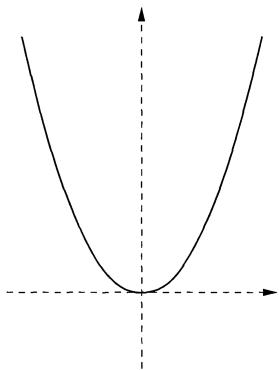
\includegraphics[width=0.42\textwidth]{figs/ch7-parabola.jpg}\qquad
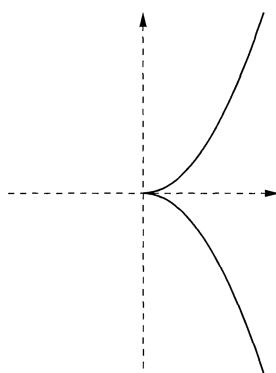
\includegraphics[width=0.42\textwidth]{figs/ch7-cusp.jpg}
\end{center}

第一个是 $\mathcal{V}((y-x^2))$; 第二个是 $\mathcal{V}((y^2-x^3))$. 理想 $(y^2-x^3)$ 的什么性质造成了第二幅图中 $(0,0)$ 处的``尖点''? 读者在任何一门初等代数几何课程中都会找到答案.
\end{example}

$\mathcal{I}$ 不满射这一事实引出了一些有趣的思考. 不是任何集合之理想的理想的标准例子是 $K[x]$ 中的 $(x^2)$: 因为凡是 $x^2$ 消失的地方, $x$ 也消失; 所以若对某个集合 $S$ 有 $x^2\in\mathcal{I}(S)$, 则也有 $x\in\mathcal{I}(S)$. 这引出下面的定义.

\begin{definition}\label{def:radical}
设 $I$ 是交换环 $R$ 中的一个理想. $I$ 的\emph{根}\index{gen@根(radical)}是理想
\[
\sqrt{I}:=\{r\in R\mid \exists k\geq 0,\ r^k\in I\}.
\]
一个理想 $I$ 是\emph{根理想}\index{gen lixiang@根理想(radical ideal)}, 如果 $I=\sqrt{I}$.
\end{definition}

读者应当验证 $\sqrt{I}$ 确实是一个理想; 它可以刻画为所有包含 $I$ 的素理想的交 (习题~\ref{ex:radical-props}).

\begin{example}\label{ex:nilradical-example}
交换环 $R$ 中的一个元素是幂零的, 当且仅当它属于理想 $(0)$ 的根 (对照习题~V.\ref{ex:nilpotent-unit}). 读者已经在习题中遇到过这个理想, 称为 $R$ 的\emph{幂零根}, 从习题~III.\ref{ex:nilradical} 开始.

素理想 $\mathfrak{p}$ 显然是根理想: 因为 $f^k\in\mathfrak{p}\implies f\in\mathfrak{p}$, 从而 $\sqrt{\mathfrak{p}}\subseteq\mathfrak{p}$ (另一个包含关系对一切理想都平凡地成立).
\end{example}

\begin{lemma}\label{lem:ideal-of-set-radical}
设 $K$ 是一个域, 并设 $S$ 是 $\mathbb{A}_K^n$ 的一个子集. 则理想 $\mathcal{I}(S)$ 是 $K[x_1,\ldots ,x_n]$ 的一个根理想.
\end{lemma}

\begin{proof}
包含关系 $\mathcal{I}(S)\subseteq\sqrt{\mathcal{I}(S)}$ 对每个理想都成立, 所以平凡地满足. 为验证包含关系 $\sqrt{\mathcal{I}(S)}\subseteq\mathcal{I}(S)$, 设 $f\in\sqrt{\mathcal{I}(S)}$. 则存在整数 $k\geq 0$ 使得 $f^k\in\mathcal{I}(S)$; 也就是说,
\[
(\forall p\in S),\quad f(p)^k=0.
\]
于是
\[
(\forall p\in S),\quad f(p)=0,
\]
这就证明了 $f\in\mathcal{I}(S)$, 正是所需要的. \qed
\end{proof}

鉴于这些考虑, 对任意域我们可以把 $\mathbb{A}_K^n$ 的子集与 $K[x_1,\ldots ,x_n]$ 的理想之间的对应精化如下:
\[
\begin{tikzcd}[column sep=3em]
\{\mathbb{A}_K^n\text{ 的代数子集}\} \ar[r,shift left=.7ex,"\mathcal I"] & \{K[x_1,\ldots ,x_n]\text{ 中的根理想}\}; \ar[l,shift left=.7ex,"\mathcal V"]
\end{tikzcd}
\]
正如我们论证过的, 如果想要有一部好的词典, 这样做是必要的. 在本节余下部分, $\mathcal{I}$ 与 $\mathcal{V}$ 将被看作在这两个集合之间作用.

虽然我们已经把这个对应大大收紧了, 情况仍不完美. 在任意域上, 函数 $\mathcal{V}$ 现在按仿射代数子集的定义是满射 (对照习题~\ref{ex:alg-set-radical-ideal}); 但它不一定是单射. 一个立刻的反例由 $K=\R$ 上的理想 $(x^2+1)$ 给出: 它是极大的, 从而是素的, 从而是根理想, 而
\[
\mathcal{V}(x^2+1)=\emptyset=\mathcal{V}(1).
\]

零点定理正是在这里来帮助我们, 而我们也正是在这里看到零点定理与一个理想的``零点'' (= 该理想的 $\mathcal{V}$) 有什么关系.

\begin{proposition}[弱零点定理]\label{prop:weak-nullstellensatz}
设 $K$ 是代数闭域, 并设 $I\subseteq K[x_1,\ldots ,x_n]$ 是一个理想. 则 $\mathcal{V}(I)=\emptyset$ 当且仅当 $I=(1)$.
\end{proposition}

\begin{proof}
若 $I=(1)$, 则按定义 $\mathcal{V}(I)=\emptyset$.

反过来, 假设 $I\neq (1)$. 由命题~V.\ref{prop:maximal-ideal-exists}, $I$ 包含在一个极大理想 $\mathfrak{m}$ 中. 由于 $K$ 是代数闭的, 由推论~\ref{cor:maximal-ideals-points} 我们有
\[
\mathfrak{m}=(x_1-c_1,\ldots ,x_n-c_n)
\]
其中 $c_1,\ldots ,c_n\in K$; 所以对每个 $f(x_1,\ldots ,x_n)\in I$ 存在 $g_1,\ldots ,g_n\in K[x_1,\ldots ,x_n]$ 使得
\[
f(x_1,\ldots ,x_n)=\sum_{i=1}^{n}g_i(x_1,\ldots ,x_n)(x_i-c_i).
\]\erratumfootnote{根据官方勘误, 公式中多项式因子记号统一修正为 $g_i$.}
特别地,
\[
f(c_1,\ldots ,c_n)=\sum_{i=1}^{n}g_i(c_1,\ldots ,c_n)(c_i-c_i)=0:
\]
也就是说, $(c_1,\ldots ,c_n)\in\mathcal{V}(I)$. 这就证明了当 $I\neq (1)$ 时 $\mathcal{V}(I)\neq\emptyset$, 证毕. \qed
\end{proof}

这令人鼓舞, 但它似乎并没有真正证明 $\mathcal{V}$ 是单射. 然而事实是, 它确实证明了: 我们可以从``弱''零点定理推出下面这个更强的结果, 而后者确实蕴涵单射性:

\begin{proposition}[强零点定理]\label{prop:strong-nullstellensatz}
设 $K$ 是代数闭域, 并设 $I\subseteq K[x_1,\ldots ,x_n]$ 是一个理想. 则
\[
\mathcal{I}(\mathcal{V}(I))=\sqrt{I}.
\]
\end{proposition}

这意味着复合 $\mathcal{I}\circ\mathcal{V}$ 在根理想集合上是恒等映射; 也就是说, $\mathcal{V}$ 有一个左逆, 从而它是单射 (对照命题~I.\ref{prop:left-right-inverse}!).

\begin{proof}
注意 $\mathcal{I}(\mathcal{V}(I))$ 是一个根理想 (由引理~\ref{lem:ideal-of-set-radical}). 由定义立刻有 $I\subseteq\mathcal{I}(\mathcal{V}(I))$; 因此
\[
\sqrt{I}\subseteq\sqrt{\mathcal{I}(\mathcal{V}(I))}=\mathcal{I}(\mathcal{V}(I)).
\]
我们必须验证反过来的包含关系: 假设 $f\in\mathcal{I}(\mathcal{V}(I))$; 也就是说, 假设
\[
f(p)=0
\]
对所有满足 $\forall g\in I,\ g(p)=0$ 的 $p\in\mathbb{A}_K^n$ 成立; 我们要证明存在 $m$ 使得 $f^m\in I$.

这个论证在事后看来并不困难, 但它极其巧妙\footnote{这称为 Rabinowitsch 技巧, 可追溯到 1929 年. 它发表于《Mathematische Annalen》上一篇仅一页、十八行的文章中.}. 令 $y$ 是一个额外的变量, 考虑 $K[x_1,\ldots ,x_n,y]$ 中由 $I$ 与 $1-fy$ 生成的理想 $J$. 更明确地, 假设
\[
I=(g_1,\ldots ,g_r)
\]
(由于 $K[x_1,\ldots ,x_n]$ 是 Noether 的, 有限多个生成元就够了); 我们可以把 $g_i(x_1,\ldots ,x_n)$ 与 $f(x_1,\ldots ,x_n)\in K[x_1,\ldots ,x_n]$ 分别看成多项式 $G_i(x_1,\ldots ,x_n,y)$ 与 $F(x_1,\ldots ,x_n,y)\in K[x_1,\ldots ,x_n,y]$, 并令
\[
J=(G_1,\ldots ,G_r,1-Fy).
\]
由于 $K[x_1,\ldots ,x_n,y]$ 有 $n+1$ 个变量, 理想 $J$ 定义了 $\mathbb{A}_K^{n+1}$ 中的一个子集 $\mathcal{V}(J)$. 我们断言 $\mathcal{V}(J)=\emptyset$.

确实, 反设 $\mathcal{V}(J)\neq\emptyset$, 并设 $p=(a_1,\ldots ,a_n,b)\in\mathbb{A}_K^{n+1}$ 是 $\mathcal{V}(J)$ 的一个点. 那么对 $i=1,\ldots ,r$ 有
\[
G_i(a_1,\ldots ,a_n,b)=0;
\]
但这意味着
\[
g_i(a_1,\ldots ,a_n)=0
\]
对 $i=1,\ldots ,r$ 成立; 也就是说, $(a_1,\ldots ,a_n)\in\mathcal{V}(I)$. 由于 $f$ 在 $\mathcal{V}(I)$ 的所有点上都消失, 这意味着
\[
f(a_1,\ldots ,a_n)=0,
\]
于是
\[
(1-Fy)(a_1,\ldots ,a_n,b)=1-f(a_1,\ldots ,a_n)b=1-0=1.
\]
但这与 $p\in\mathcal{V}(J)$ 的假设矛盾. 因此 $\mathcal{V}(J)=\emptyset$.

现在使用弱零点定理: 由于 $K$ 是代数闭的, 我们可以断定 $J=(1)$. 因此存在多项式 $H_i(x_1,\ldots ,x_n,y)$ ($i=1,\ldots ,r$) 与 $L(x_1,\ldots ,x_n,y)$, 使得
\[
\sum_{i=1}^{r}H_i(x_1,\ldots ,x_n,y)G_i(x_1,\ldots ,x_n,y)+L(x_1,\ldots ,x_n,y)\bigl(1-F(x_1,\ldots ,x_n,y)y\bigr)=1.
\]
我们的巧妙还没有结束: 下一步是在 $K$ 上的有理函数域中 (而不是在多项式环中) 看待这个等式, 我们这样做是可以的, 因为后者是前者的子环. 于是我们可以代入 $y=1/F$ 而仍然得到一个等式, 好处是消掉了左边最后一项:
\[
\sum_{i=1}^{r}H_i\left(x_1,\ldots ,x_n,\frac{1}{F}\right)G_i\left(x_1,\ldots ,x_n,\frac{1}{F}\right)=1.
\]
进而,
\[
G_i\left(x_1,\ldots ,x_n,\frac{1}{F}\right)=g_i(x_1,\ldots ,x_n)
\]
($G_i$ 只是 $g_i$ 在更大的多项式环中的名字, 并且只依赖前 $n$ 个变量), 而
\[
H_i\left(x_1,\ldots ,x_n,\frac{1}{F}\right)=\frac{h_i(x_1,\ldots ,x_n)}{f(x_1,\ldots ,x_n)^m},
\]
其中 $h_i\in K[x_1,\ldots ,x_n]$, 而 $m$ 是一个大到对所有 $i=1,\ldots ,r$ 都适用的整数. 用通分表示, 我们可以把这个恒等式重写为
\[
\frac{h_1g_1+\cdots +h_rg_r}{f^m}=1,
\]
或
\[
f^m=h_1g_1+\cdots +h_rg_r.
\]
我们是在有理函数域中证明这个恒等式的; 由于它只涉及多项式, 它在 $K[x_1,\ldots ,x_n]$ 中成立. 右边是 $I$ 的一个元素, 所以这证明了 $f\in\sqrt{I}$, 证毕. \qed
\end{proof}

证明中添加变量 $y$ 的做法, 如果从几何角度来看, 就显得更合理 (也不那么像一个花招). $\mathbb{A}_K^2$ 中的簇 $\mathcal{V}(1-xy)$ 是一条普通的双曲线:

\begin{center}
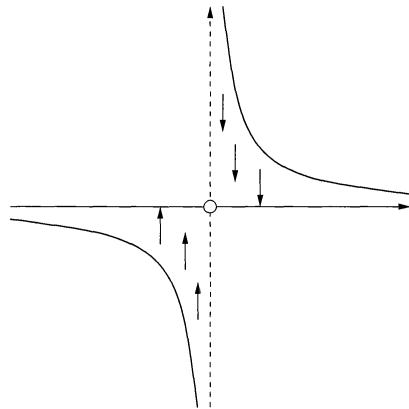
\includegraphics[width=0.5\textwidth]{figs/ch7-hyperbola.jpg}
\end{center}

投影 $(x,y)\mapsto x$ 可用来把 $\mathcal{V}(1-xy)$ 与``$x$ 轴'' (看作 $\mathbb{A}_K^1$) 中原点 (即 $\mathcal{V}(x)$) 的补集等同起来. 类似地, $\mathcal{V}(1-fy)$ 是把 Zariski 开集 $\mathbb{A}_K^n\setminus\mathcal{V}(f)$ 实现为维数高一维的空间 $\mathbb{A}_K^{n+1}$ 中一个 Zariski 闭子集的一种方式.

命题~\ref{prop:strong-nullstellensatz} 的证明正依赖于这个事实, 而这个事实也是代数几何基本框架中的一个重要构件, 因为它可以用来证明 Zariski 拓扑有一组由 (在适当意义上同构于) 仿射代数集的集合构成的基.

我们将正式记录下关于函数 $\mathcal{V}$ 与 $\mathcal{I}$ 所能确立的结论:

\begin{corollary}\label{cor:agc-dictionary}
设 $K$ 是代数闭域. 则对任意 $n\geq 0$, 函数
\[
\begin{tikzcd}[column sep=3em]
\{\mathbb{A}_K^n\text{ 的代数子集}\} \ar[r,shift left=.7ex,"\mathcal I"] & \{K[x_1,\ldots ,x_n]\text{ 中的根理想}\} \ar[l,shift left=.7ex,"\mathcal V"]
\end{tikzcd}
\]
互为逆映射.
\end{corollary}

\begin{proof}
命题~\ref{prop:strong-nullstellensatz} 表明 $\mathcal{I}\circ\mathcal{V}$ 在根理想上是恒等映射, 所以 $\mathcal{V}$ 是单射, 而 $\mathcal{V}$ 按仿射代数集的定义是满射. 由此 $\mathcal{V}$ 是双射而 $\mathcal{I}$ 是它的逆. \qed
\end{proof}

\noindent\emph{总结.} 若 $K$ 是代数闭的, 则在空间 $K^n$ 中研究由多项式方程定义的集合, 与在多项式环 $K[x_1,\ldots ,x_n]$ 中研究根理想是``同一件事''.

这个对应实际上在 $K$-代数的层面上实现得更为有效. 我们说一个环是\emph{既约的}\index{jiyue@既约的(reduced)}, 如果它没有非零的幂零元; 于是 $R/I$ 是既约的当且仅当 $I$ 是根理想 (习题~\ref{ex:radical-props}).

\begin{definition}\label{def:coordinate-ring}
设 $S\subseteq\mathbb{A}_K^n$ 是一个代数集. $S$ 的\emph{坐标环}\index{zuobiaohuan@坐标环(coordinate ring)}是商\footnote{记号 $K[S]$ 相当标准, 尽管它可能与通常的多项式环记号混淆; 希望上下文足以消除歧义. 把域的名字写在记号中是合理的, 因为原则上可以改变基域, 同时保留理想 $\mathcal I(S)$ 所编码的``相同''方程.}
\[
K[S]:=\frac{K[x_1,\ldots ,x_n]}{\mathcal{I}(S)}.
\]
\end{definition}

\index{daishujidezuobiaohuan@代数集的坐标环(coordinate ring of an algebraic set)}于是, 一个代数集的坐标环是一个既约的、有限型的交换 $K$-代数. 读者将在习题~\ref{ex:polynomial-functions} 中建立这个环的一个``具体''解释, 即作为 $S$ 上``多项式函数''的环. 理解零点定理 (以其作为推论~\ref{cor:agc-dictionary} 的表现形式) 的一种方式是这样: 若 $K$ 是代数闭的, 则每个有限型既约交换 $K$-代数 $R$ 都可以实现为某个仿射代数集 $S$ 的坐标环; $S$ 的点以一种自然的方式对应于 $R$ 的极大理想 (习题~\ref{ex:points-maximal-ideals}).

事实上\footnote{这当然是对实际情况的极度简化.}, 在基础代数几何中, 人们正是通过这一对应来定义一个域 $K$ 上的仿射代数集的范畴: 代数集的态射被定义为与相应的 (既约、有限型) $K$-代数的同态相匹配. (读者将在例~VIII.\ref{ex:k-aff} 中遇到一个更精确的定义.)

这部词典使我们能够把一个代数集的每个``几何''特征 (例如维数、光滑性等等) 翻译成相应的坐标环的对应``代数''特征. 一旦这些关键的代数特征被辨认出来, 人们就可以抛开``在代数闭域上的既约有限型代数上工作''这一限制, 尝试在任意 (比如说交换的、Noether 的) 环上``做几何''. 例如, 结果发现 PID 对应于仿射几何世界中的 (某些) 光滑曲线; 于是人们可以尝试把 $\Z$ 想象成一条``光滑曲线'' (尽管 $\Z$ 不是任何域 $K$ 上的既约有限型 $K$-代数!) 并尝试使用受曲线几何启发的定理来理解 $\Z$ 的特征——也就是说, 用几何来做数论.

\index{pu@谱(spectrum)!huande@环的(of a ring)}这些简单的考虑可以被推广的另一个方向, 是通过把仿射代数集``粘合''成类似流形的对象: 这些集合在``整体''上可能不是仿射代数集, 但可以被仿射代数集覆盖. 做这件事的一个具体办法是在射影空间而不是仿射空间中工作; 整体化的过程于是可以在代数层面以一种直接的方式进行, 在那里它被翻译为对``分次''环与模的研究——更多遗憾地在我们这本书中找不到位置的概念 (只在 §VIII.\ref{subsec:graded-algebra} 中匆匆一瞥). 在二十世纪下半叶, 一个由 Alexander Grothendieck 等人倡导的更抽象的观点被证明极为有效; 它导致了对概形\index{guaixing@概形(scheme)}——代数几何当今通用的语言——的深入研究. 我们早在 §III.\ref{subsec:prime-maximal-def} 引入环的谱 $\Spec R$ 时, 就已经遇到过最简单的一类概形.

\subsection*{习题}
\phantomsection
\addcontentsline{toc}{subsection}{习题}

\begin{prob}\label{ex:alg-closed-equiv-proof}
$\triangleright$ 证明引理~\ref{lem:alg-closed-equiv}. [§\ref{subsec:algebraic-closure}]
\end{prob}

\begin{prob}\label{ex:alg-closure-minimal}
$\triangleright$ 设 $k\subseteq\overline{k}$ 是一个代数闭包, 并设 $L$ 是一个中间域. 假设每个多项式 $f(x)\in k[x]\subseteq L[x]$ 都在 $L[x]$ 中分解为一次因子的乘积. 证明 $L=\overline{k}$. [§\ref{subsec:algebraic-closure}]
\end{prob}

\begin{prob}\label{ex:countable-closure}
证明若 $k$ 是可数域, 则 $\overline{k}$ 也是可数的.
\end{prob}

\begin{prob}\label{ex:partial-fractions-nonzero}
$\triangleright$ 设 $k$ 是一个域, 设 $c_1,\ldots ,c_m\in k$ 是互异元素, 并设 $\lambda_1,\ldots ,\lambda_m$ 是 $k$ 的非零元素. 证明
\[
\frac{\lambda_1}{x-c_1}+\cdots +\frac{\lambda_m}{x-c_m}\neq 0.
\]
(这个事实用在定理~\ref{thm:nullstellensatz} 的证明中.) [§\ref{subsec:nullstellensatz}]
\end{prob}

\begin{prob}\label{ex:V-of-ideal-generated}
$\triangleright$ 设 $K$ 是一个域, 设 $A$ 是 $K[x_1,\ldots ,x_n]$ 的一个子集, 并设 $I$ 是 $A$ 生成的理想. 证明在 $\mathbb{A}_K^n$ 中 $\mathcal{V}(A)=\mathcal{V}(I)$. [§\ref{subsec:affine-geometry}]
\end{prob}

\begin{prob}\label{ex:non-algebraic-subsets}
$\triangleright$ 设 $K$ 是你最喜欢的无限域. 找出不能实现为任何理想 $I\subseteq K[x_1,\ldots ,x_n]$ 的 $\mathcal{V}(I)$\erratumfootnote{根据官方勘误, 原书此处规范代数集算子符号为花体字形 $\mathscr{V}(I)$.} 的子集 $S\subseteq\mathbb{A}_K^n$ 的例子. 证明若 $K$ 是有限域, 则每个子集 $S\subseteq\mathbb{A}_K^n$ 都等于某个理想 $I\subseteq K[x_1,\ldots ,x_n]$ 的 $\mathcal{V}(I)$. [§\ref{subsec:affine-geometry}]
\end{prob}

\begin{prob}\label{ex:zariski-topology}
$\triangleright$ 设 $K$ 是一个域而 $n$ 是一个非负整数. 证明 $\mathbb{A}_K^n$ 的代数子集族是 $\mathbb{A}_K^n$ 上某个拓扑的闭集族. [§\ref{subsec:affine-geometry}]
\end{prob}

\begin{prob}\label{ex:radical-props}
$\triangleright$ 采用定义~\ref{def:radical} 中的记号:
\begin{itemize}
\item 证明集合 $\sqrt{I}$ 是 $R$ 的一个理想.
\item 通过 $R/I$ 的理想与 $R$ 中包含 $I$ 的理想之间的对应, 证明 $\sqrt{I}$ 对应于 $R/I$ 的幂零根.
\item 证明 $\sqrt{I}$ 事实上是所有包含 $I$ 的 $R$ 的素理想的交. (对照习题~V.\ref{ex:nilradical-prime-intersection}.)
\item 证明 $I$ 是根理想当且仅当 $R/I$ 是既约的. (对照习题~III.\ref{ex:reduced}.)
\end{itemize}
[§\ref{subsec:affine-geometry}]
\end{prob}

\begin{prob}\label{ex:alg-set-radical-ideal}
$\triangleright$ 证明每个仿射代数集都等于某个根理想 $I$ 的 $\mathcal{V}(I)$. [§\ref{subsec:affine-geometry}]
\end{prob}

\begin{prob}\label{ex:noetherian-power-radical}
\index{Noether@Noether!huan@环(ring)}证明 Noether 环中的每个理想都含有它的根的某个幂.
\end{prob}

\begin{prob}\label{ex:reduced-not-coordinate}
假设一个域不是代数闭的. 找出一个既约的有限型 $K$-代数, 它不是任何仿射代数集的坐标环.
\end{prob}

\begin{prob}\label{ex:polynomial-functions}
$\triangleright$ 设 $K$ 是无限域. 仿射代数集 $S\subseteq\mathbb{A}_K^n$ 上的一个\emph{多项式函数}, 是一个多项式 $f(x_1,\ldots ,x_n)\in K[x_1,\ldots ,x_n]$ 的 (求值函数的) 在 $S$ 上的限制. 代数集 $S$ 上的多项式函数显然构成一个环, 而且事实上是一个 $K$-代数. 证明这个 $K$-代数同构于 $S$ 的坐标环. [§\ref{subsec:affine-geometry}, §VIII.\ref{subsec:equiv-categories}, §VIII.\ref{subsec:tensor-flatness}]
\end{prob}

\begin{prob}\label{ex:reduced-fg-is-coordinate}
设 $K$ 是代数闭域. 证明每个有限型既约交换 $K$-代数都是某个仿射空间 $\mathbb{A}_K^n$ 中一个代数集 $S$ 的坐标环.
\end{prob}

\begin{prob}\label{ex:points-maximal-ideals}
$\triangleright$ 证明在代数闭域 $K$ 上, 一个代数集 $S$ 的点对应于坐标环 $K[S]$ 的极大理想, 并且若 $p$ 对应于极大理想 $\mathfrak{m}_p$, 则函数 $f\in K[S]$ 在 $p$ 处的值等于 $f$ 在 $K[S]/\mathfrak{m}_p\cong K$ 中的陪集. [§\ref{subsec:affine-geometry}, VIII.\ref{ex:k-aff-points}]
\end{prob}

\begin{prob}\label{ex:irreducible-prime}
$\neg$ 设 $K$ 是代数闭域. $\mathbb{A}_K^n$ 的一个代数子集 $S$ 是\emph{不可约的}\index{bukeyue@不可约的(irreducible)}, 如果它不能写成两个真包含于它的代数子集的并. 证明 $S$ 不可约当且仅当它的理想 $\mathcal{I}(S)$ 是素理想, 当且仅当它的坐标环 $K[S]$ 是整环.

不可约代数集``浑然一体'', 就像 $\mathbb{A}_K^n$ 自己那样, 而不像 (例如) 以 $x,y$ 为坐标的仿射平面 $\mathbb{A}_K^2$ 中的 $\mathcal{V}(xy)$. 不可约的仿射代数集称为\emph{(仿射代数) 簇}. [\ref{ex:cusp-coordinate-rings}]
\end{prob}

\begin{prob}\label{ex:rational-functions-localization}
$\triangleright$ 设 $K$ 是代数闭域. 有理函数域 $K(x_1,\ldots ,x_n)$ 是 $K[\mathbb{A}_K^n]=K[x_1,\ldots ,x_n]$ 的分式域; 每个有理函数 $\alpha=F/G$ (其中 $G\neq 0$ 且 $F,G$ 互素) 都可以看作在开集 $\mathbb{A}_K^n\setminus\mathcal{V}(G)$ 上定义了一个函数; 我们说 $\alpha$ 对 $\mathcal{V}(G)$ 的补集中的所有点都``有定义''.

设 $G\in K[x_1,\ldots ,x_n]$ 不可约. 在 $\mathcal{V}(G)$ 的补集中有定义的有理函数的集合是 $K(x_1,\ldots ,x_n)$ 的一个子环. 证明这个子环可以等同于 $K[\mathbb{A}_K^n]$ 在乘性集合 $\{1,G,G^2,G^3,\ldots \}$ 处的局部化 (习题~V.\ref{ex:localization-ring}). (使用零点定理.)
[\ref{ex:germs-localization}, \ref{ex:rational-function-fields-curves}, \S\ref{subsec:ft-galois-II}]
\end{prob}

\begin{prob}\label{ex:germs-localization}
$\neg$ 设 $K$ 是代数闭域, 并设 $\mathfrak{m}$ 是 $K[x_1,\ldots ,x_n]$ 的一个极大理想, 对应于 $\mathbb{A}_K^n$ 的一个点 $p$. 一个函数在 $p$ 处的\emph{芽}\index{ya@芽(germ)}, 由一个包含 $p$ 的开集以及定义在该开集上的一个函数确定; 在我们的语境中 (处理有理函数, 并且开集可以取为一个在 $p$ 处不消失的函数的补集), 这与一个在 $p$ 处有定义的有理函数 (在习题~\ref{ex:rational-functions-localization} 的意义下) 是同一份信息.

说明如何把芽环等同于局部化 $K[\mathbb{A}_K^n]_{\mathfrak{m}}$ (在习题~V.\ref{ex:local-ring} 中定义).

如同习题~\ref{ex:rational-functions-localization} 那样, 同样的讨论可以对任意代数集进行. 这就是``局部化''这个名字的由来: 把一个簇 $V$ 的坐标环在对应于点 $p$ 的极大理想处局部化, 相当于只考虑在 $p$ 的某个邻域中有定义的函数, 从而也就是在 $p$ ``附近''``局部地''研究 $V$. [V.\ref{ex:localization-ring}]
\end{prob}

\begin{prob}\label{ex:cusp-coordinate-rings}
$\neg$ 设 $K$ 是代数闭域. 考虑 $\mathbb{A}_K^2$ 中的两条``曲线'' $C_1:y=x^2$ 与 $C_2:y^2=x^3$ (这些代数集的实点图像见例~\ref{ex:cusp}).
\begin{itemize}
\item 证明 $K[C_1]\cong K[t]=K[\mathbb{A}_K^1]$, 而 $K[C_2]$ 可以等同于 $K[t]$ 的由 $t$-系数为零的多项式 $a_0+a_2t^2+\cdots +a_dt^d$ 组成的子环 $K[t^2,t^3]$. (注意 $K[x,y]$ 中每个多项式都可以唯一地写成 $f(x)+g(x)y+h(x,y)(y^2-x^3)$ 的形式, 其中 $f(x)$, $g(x)$, $h(x,y)$ 由该多项式唯一确定.)
\item 证明 $C_1$, $C_2$ 都是不可约的 (对照习题~\ref{ex:irreducible-prime}).
\item 证明 $K[C_1]$ 是 UFD, 而 $K[C_2]$ 不是.
\item 证明 $K[C_1]$ 与 $K[C_2]$ 的 Krull 维数都是 $1$. (这就是为什么这些集合会被称为``曲线''. 你可以使用如下事实: $K[x,y]$ 中的素理想极大链长度为 $2$.)
\item 原点 $(0,0)$ 同时在 $C_1$ 与 $C_2$ 中, 并且分别对应于 $K[C_1]$ 与 $K[C_2]$ 中由 $x$ 与 $y$ 的陪集生成的极大理想 $\mathfrak{m}_1$ 与 $\mathfrak{m}_2$.
\item 证明局部化 $K[C_1]_{\mathfrak{m}_1}$ 是一个 DVR (习题~V.\ref{ex:pid-localization-dvr}). 证明局部化 $K[C_2]_{\mathfrak{m}_2}$ 不是 DVR. (注意关系 $y^2=x^3$ 在这个环中仍然成立; 证明 $K[C_2]_{\mathfrak{m}_2}$ 不是 UFD.)
\end{itemize}
DVR 容许一个局部参数, 即它的极大理想的一个生成元 (对照习题~V.\ref{ex:dvr-pid-localparam}), 这个事实是如下几何事实的一个很好的代数翻译: 像 $C_1$ 这样的一条曲线在 $(0,0)$ 处只有一条光滑的分支. $K[C_2]_{\mathfrak{m}_2}$ 的极大理想不能只由一个元素生成, 读者可以自行验证. [\ref{ex:rational-function-fields-curves}]
\end{prob}

\begin{prob}\label{ex:rational-function-fields-curves}
证明习题~\ref{ex:cusp-coordinate-rings} 中曲线 $C_1$ 与 $C_2$ 的有理函数域 (习题~\ref{ex:rational-functions-localization}) 同构, 并且它们在 $k$ 上的超越次数都是 $1$ (对照习题~\ref{ex:transcendence-basis}).

这是我们应当把 $C_1$ 与 $C_2$ 看作``曲线''的另一个理由. 事实上, 可以证明一个簇的坐标环的 Krull 维数等于它的有理函数域的超越次数. 这是交换代数的一块基石——Noether 归一化定理——的一个推论.
\end{prob}

\begin{prob}\label{ex:projective-cover}
$\neg$ 回顾习题~VI.\ref{ex:grassmannian-cells}: $\mathbb{P}_K^n$ 表示参数化向量空间 $K^{n+1}$ 中直线的``射影空间''. 每条这样的直线由某个非零向量 $(c_0,\ldots ,c_n)\in K^{n+1}$ 的所有倍数组成, 于是 $\mathbb{P}_K^n$ 可以等同于 $K^{n+1}\setminus\{(0,\ldots ,0)\}$ 关于等价关系 $\sim$ 的商 (在 §I.\ref{subsec:equivalence-relations} 的集合论意义下), 其中 $\sim$ 定义为\index[sym1]{46@$\mathbb{P}_K^n$}
\[
(c_0,\ldots ,c_n)\sim (c_0',\ldots ,c_n')\iff (\exists \lambda\in K^{*}),\ (c_0',\ldots ,c_n')=(\lambda c_0,\ldots ,\lambda c_n).
\]
由向量 $(c_0,\ldots ,c_n)$ 确定的 $\mathbb{P}_K^n$ 中的``点''记作 $(c_0:\cdots :c_n)$; 这些是该点的``射影坐标''\footnote{这是方便的记号滥用. 请记住, $c_i$ 并不由这个点确定, 因而严格来说并不是``坐标''; 不过它们的比值由这个点确定.}. 注意不存在``点'' $(0:\cdots :0)$.\index[sym1]{09@$(c_0:\cdots:c_n)$}

证明由
\[
(c_1,\ldots ,c_n)\mapsto (1:c_1:\cdots :c_n)
\]
定义的函数 $\mathbb{A}_K^n\to\mathbb{P}_K^n$ 是到其像上的双射\erratumfootnote{根据官方勘误, 原书英文此处由 ``is a bijection'' 修正为 ``is a bijection onto its image''.}. 这个函数被用来把 $\mathbb{A}_K^n$ 实现为 $\mathbb{P}_K^n$ 的一个子集. 通过使用类似的函数, 证明 $\mathbb{P}_K^n$ 可以被 $n+1$ 份 $\mathbb{A}_K^n$ 的拷贝覆盖, 并把这个事实与习题~VI.\ref{ex:grassmannian-cells} 中得到的胞腔分解联系起来. (建议: 仔细地做一遍 $n=2$ 的情形.) [\ref{ex:projective-algebraic-set}, VIII.\ref{ex:plucker-equations}]
\end{prob}

\begin{prob}\label{ex:projective-algebraic-set}
$\neg$ 设 $F(x_0,\ldots ,x_n)\in K[x_0,\ldots ,x_n]$ 是一个齐次多项式. 采用习题~\ref{ex:projective-cover} 中的记号, 证明对点 $(c_0:\cdots :c_n)\in\mathbb{P}_K^n$ 而言条件``$F(c_0,\ldots ,c_n)=0$''是良定义的: 它不依赖于为该点所选取的代表元 $(c_0,\ldots ,c_n)$. 于是我们可以定义 $\mathbb{P}_K^n$ 的如下子集:
\[
\mathcal{V}(F):=\{(c_0:\cdots :c_n)\in\mathbb{P}_K^n\mid F(c_0,\ldots ,c_n)=0\}.
\]
证明这个``射影代数集''可以被 $n+1$ 个仿射代数集覆盖.

``射影代数几何''中的基本定义可以沿着与本节为仿射代数几何所走的道路本质相同的路线来发展, 只不过使用``齐次理想'' (即由齐次多项式生成的理想; 见 §VIII.\ref{subsec:graded-algebra}) 而不是普通的理想. 这道习题展示了在一个模板例子中把射影代数集与仿射代数集联系起来的一种方式. [VIII.\ref{ex:plucker-equations}, VIII.\ref{ex:projective-variety}]
\end{prob}

\section{几何不可能性}
\label{sec:geometric-impossibilities}

域论中一些非常简单的考察, 就能轻松了结一大类长期以来似乎无从下手的几何问题——这些问题曾困扰希腊人, 直到相对晚近才被解决.

\index{chiguizuotu@尺规作图(straightedge-and-compass constructions)}这些问题关乎用``直尺与圆规'' (亦即服从某些非常严格的规则) 去作某些几何图形. 这些作图的实际用途看来绝对为零, 但是, 对于那些曾经难住了极其聪明的头脑、而我们如今却能彻底理解的事情, 由此获得的智识上的满足, 值得为此小小的绕道一行.

\subsection{直尺与圆规作图}
\label{subsec:straightedge-compass}

我们从普通实平面上的两个点 $O$, $P$ 出发. 允许你在平面中标记 (``作'') 更多的点与其他几何图形, 但只能依照下列规则:

\begin{itemize}
\item 如果你已经作出了两个点 $A$, $B$, 那么你可以作过这两点的直线 (用你的直尺).
\item 如果你已经作出了两个点 $A$, $B$, 那么你可以作以 $A$ 为圆心且经过 $B$ 的圆 (用你的圆规).
\item 你可以标记任意多个你已经作出的两条不同直线, 一条直线和一个圆, 或两个不同圆的交点.
\end{itemize}

施行这些动作会产生复杂 (而优美) 的直线与圆的集合; 如果某个图形作为整个画面的一部分出现, 我们就说我们``作出了''它.

例如, 下面是用 $O$, $P$ 作为其中两个顶点来作等边三角形的一个方案:

\begin{enumerate}
\item[(1)] 作以 $O$ 为圆心, 经过 $P$ 的圆;
\item[(2)] 作以 $P$ 为圆心, 经过 $O$ 的圆;
\item[(3)] 令 $Q$ 为这两个圆的两个交点中的任意一个;
\item[(4)] 作过 $O$, $P$; 过 $O$, $Q$; 以及过 $P$, $Q$ 的直线.
\end{enumerate}

\begin{center}
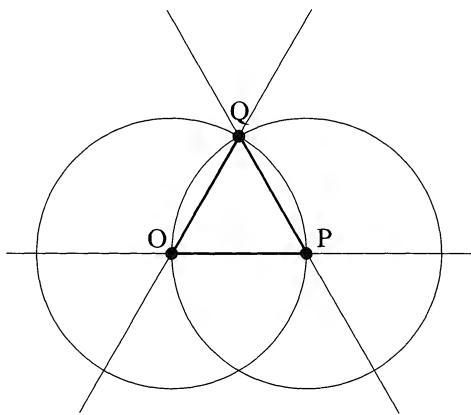
\includegraphics[width=0.5\textwidth]{figs/ch7s3-01.jpg}
\end{center}

当然, $O$, $P$, $Q$ 是一个等边三角形的顶点.

尝试给出作出某个给定图形或几何构型的具体的基本步骤序列, 是一个愉快的练习. 富有进取心的读者可以在不查资料, 并且在我们学到足够多以至于挫败纯粹几何直觉之前, 试着用直尺与圆规作出正五边形的顶点.

一般的问题是判断一个图形能不能用这种方式作出. 下述三类问题在古代就声名远扬:

\begin{itemize}
\item 三等分角;
\item 化圆为方;
\item 倍立方.
\end{itemize}

例如, 假设已经作出了两条形成角 $\theta$ 的直线, 问能否作出两条形成角 $\theta/3$ 的直线. 对某些可构造的 $\theta$ 这显然是可能的: 我们刚刚作出了一个 $\pi/3$ 的角, 所以显然我们能够三等分角 $\pi$; 但是这对所有可构造的角都能做到吗?

\index{kegouzao@可构造(constructible)}答案是否定的. 类似地, 不可能作出与一个 (可构造的) 圆面积相同的正方形, 也不可能作出边长等于一个给定 (可构造) 边长立方体之体积两倍的立方体的棱.

\index{zhengduobianxing@正多边形(regular polygon)!dekegouzaoxing@的可构造性(constructibility of a)}域论将使我们能够确立这一切\footnote{不过, 为证明化圆为方不可能, 我们将用到 $\pi$ 的超越性; 本书不证明这一事实.}.\index{zhichi yu yuan gui@直尺与圆规(straightedge and compass)} 稍后我们会回到这些作图, 并研究给定边长的正多边形的可构造性问题: 用直尺与圆规作出等边三角形 (我们刚刚做过), 正方形, 正六边形都极易; 作出正五边形也不太难; 但是哪些多边形可构造, 哪些不可构造, 却与域论中更深刻的问题优美地联系在一起.

上述三类问题有一段显赫的历史; 如果阿里斯托芬《鸟》中的这一残篇可作凭据, 它们至少可以追溯到公元前414年:

\begin{quote}
METON: 用直尺一量, 这圆就成了一个带内院的方.\footnote{感谢 Matilde Marcolli 提供翻译. 对于比我更懂希腊语的读者, 原文是: {\fontspec{LibertinusSerif-Regular.otf} ὀρθῶι μετρήσω κανόνι προστιθείς ἵνα / ὁ κύκλος γένηταί σοι τετράγωνος κἀν μέσωι / ἀγορά.}}
\end{quote}

\index{Archimedes@Archimedes}这些问题的答案依赖于施加在作图上的精确限制. 例如, 如果允许在直尺上做标记 (从而把它变成一把``标尺''), 那么三等分角是可以做到的; 事实上, 这一点阿基米德已经知道 (习题~\ref{ex:archimedes-trisection}).

把这些几何问题翻译成代数, 需要先确立若干基本作图的可行性.

首先, 可以作过给定点 $A$ 且垂直于给定直线 $\ell$ 的直线 (于是 $\ell$ 至少还包含另一个可构造点 $B$). 为此, 作以 $A$ 为圆心且经过 $B$ 的圆;

——如果这个圆只在 $B$ 处与 $\ell$ 相交, 那么过 $A$ 与 $B$ 的直线就垂直于 $\ell$:

\begin{center}
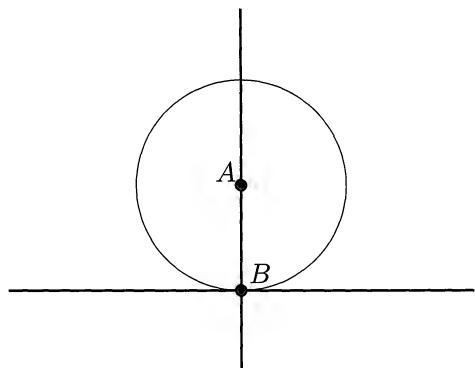
\includegraphics[width=0.42\textwidth]{figs/ch7s3-02.jpg}
\end{center}

——否则, 这个圆在第二个点 $C$ 处与 $\ell$ 相交 (无论 $A$ 是否在 $\ell$ 上):

\begin{center}
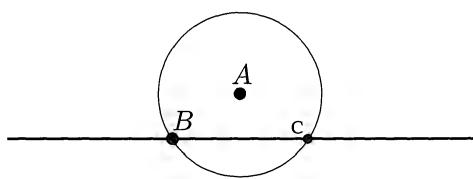
\includegraphics[width=0.42\textwidth]{figs/ch7s3-03.jpg}
\end{center}

一旦确定了 $C$, 过 $A$ 且垂直于 $\ell$ 的直线就可以通过连接分别以 $B$, $C$ 为圆心且经过 $C$, $B$ 的两个圆的两个交点 $D$, $E$ 而得到:

\begin{center}
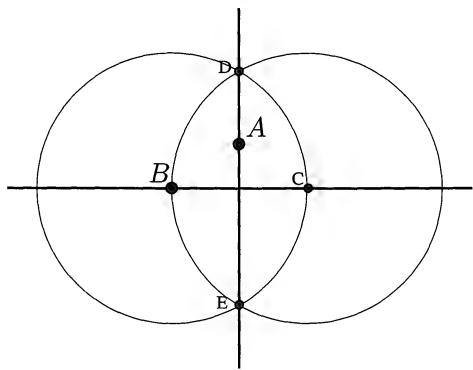
\includegraphics[width=0.42\textwidth]{figs/ch7s3-04.jpg}
\end{center}

对这个作图施用两次, 就得到过一点 $A$ 且平行于一条给定直线的直线:

\begin{center}
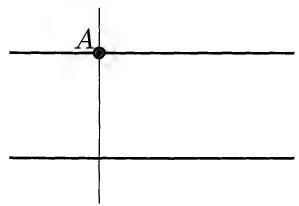
\includegraphics[width=0.42\textwidth]{figs/ch7s3-05.jpg}
\end{center}

这常常很方便.

对这些运算的审慎应用, 使我们能把一个笛卡儿坐标系引入画面. 从初始的两个点 $O$, $P$ 出发, 我们可以作出以 $O$ 为中心, 互相垂直的笛卡儿坐标轴, 并令 $P$ 标记 (比如说) ``$x$ 轴''上的点 $(1,0)$:

\begin{center}
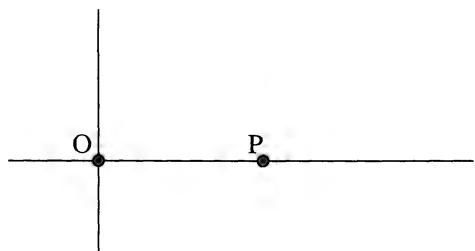
\includegraphics[width=0.5\textwidth]{figs/ch7s3-06.jpg}
\end{center}

而作一个点 $A=(x,y)$ 等价于作它在坐标轴上的投影 $X=(x,0)$, $Y=(0,y)$, 事实上又等价于作两个点 $X=(x,0)$ 与 $Y'=(y,0)$:

\begin{center}
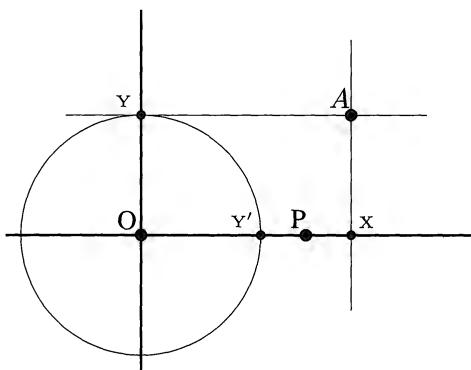
\includegraphics[width=0.5\textwidth]{figs/ch7s3-07.jpg}
\end{center}

\index{kegouzao@可构造(constructible)!jihetuxing@几何图形(geometric figures)}由此可见, 判定哪些图形能用直尺与圆规构造, 等价于判定哪些数可以作为一个可构造点的坐标来实现.

\index{kegouzao@可构造(constructible)!zhengduobianxing@正多边形(regular polygon)}\index{kegouzao@可构造(constructible)!shu@数(number)}\begin{definition}\label{def:constructible}
一个实数 $r$ 是\emph{可构造的}\index{ke gou zao@可构造的(constructible)}, 如果 (在上面取 $O=(0,0)$, $P=(1,0)$ 的意义下) 点 $(r,0)$ 能用直尺与圆规构造. 我们以 $\mathcal{C}_{\mathbb{R}}\subseteq\mathbb{R}$ 表示可构造实数之集.
\end{definition}

同样, 我们可以把实平面与 $\mathbb{C}$ 等同, 把 $O$ 放在 $0$, $P$ 放在 $1$, 并且说 $z=x+iy$ 是可构造的, 如果点 $(x,y)$ 能用直尺与圆规构造. 我们以 $\mathcal{C}_{\mathbb{C}}\subseteq\mathbb{C}$ 表示可构造复数之集. 总结前面的讨论, 我们证明了:

\begin{lemma}\label{lem:constructible-point}
点 $(x,y)$ 能用直尺与圆规构造, 当且仅当 $x+iy\in\mathcal{C}_{\mathbb{C}}$, 当且仅当 $x,y\in\mathcal{C}_{\mathbb{R}}$.
\end{lemma}

下一个显然的问题是这些可构造数之集携带何种结构, 这促使我们去看更多的几个基本直尺—圆规作图.

\begin{lemma}\label{lem:constructible-field}
可构造数之集 $\mathcal{C}_{\mathbb{R}}\subseteq\mathbb{R}$ 是 $\mathbb{R}$ 的一个子域. 类似地, $\mathcal{C}_{\mathbb{C}}$ 是 $\mathbb{C}$ 的一个子域, 而且事实上 $\mathcal{C}_{\mathbb{C}}=\mathcal{C}_{\mathbb{R}}(i)$.
\end{lemma}

\begin{proof}
$C_{\mathbb{R}}\subseteq\mathbb{R}$ 非空, 所以为了说明它是一个域, 我们只需证明它对减法以及除以一个非零可构造数封闭 (参见命题~II.\ref{prop:subgroup-criterion}).

读者将验证 $C_{\mathbb{R}}$ 对减法封闭 (习题~\ref{ex:construct-difference}). 为了看出 $C_{\mathbb{R}}$ 对除法封闭, 设 $a,b\in C_{\mathbb{R}}$, 且 $b\neq 0$. 由于按假设 $A=(0,a)$ 与 $B=(b,0)$ 可构造, 我们可以如上图\footnote{图中假设 $a>0$, $b>1$; 读者可以验证其他可能情形给出相同结论.} 那样, 把 $C$ 构造为过 $P=(1,0)$ 且平行于过 $A$, $B$ 的直线的直线与 $y$ 轴的交点:

\begin{center}
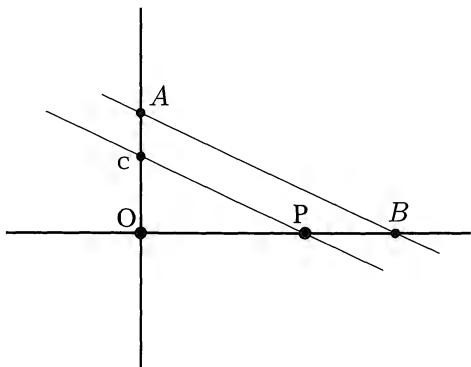
\includegraphics[width=0.42\textwidth]{figs/ch7s3-08.jpg}
\end{center}

由于三角形 $AOB$ 与 $COP$ 相似, 我们看到 $C=(0,a/b)$; 从而 $a/b$ 可构造.

$C_{\mathbb{C}}$ 是 $\mathbb{C}$ 的子域这一事实, 是 $C_{\mathbb{R}}$ 是域这一事实的直接推论, 其证明留给读者享受 (习题~\ref{ex:constructible-subfield-C}). 而 $\mathcal{C}_{\mathbb{C}}=\mathcal{C}_{\mathbb{R}}(i)$ 这个说法, 无非是重新表述了 ``$x+iy\in C_{\mathbb{C}}$ 当且仅当 $x$ 与 $y$ 都属于 $C_{\mathbb{R}}$'' 这一事实. \qed
\end{proof}

我们可以把 $C_{\mathbb{R}}$ 与 $C_{\mathbb{C}}$ 看作 $\mathbb{Q}$ 的扩张, 从而在直尺—圆规可构造性与域论之间架起一座桥: 如果我们能理解域扩张
\[
\mathbb{Q}\subseteq\mathcal{C}_{\mathbb{R}}\subseteq\mathcal{C}_{\mathbb{C}}
\]
就能理解几何图形的可构造性.

令人高兴的是, 我们能够理解这些扩张!

\subsection{可构造数与二次扩张}
\label{subsec:constructible-quadratic}

我们的目标是要证明下列关于 $C_{\mathbb{R}}$ (并从而立即给出 $C_{\mathbb{C}}$) 的惊人明确的描述.

\begin{theorem}\label{thm:constructible-quadratic}
设 $\gamma\in\mathbb{R}$. 则 $\gamma\in\mathcal{C}_{\mathbb{R}}$ 当且仅当存在实数 $\delta_1,\ldots,\delta_k$, 使得对所有 $j=1,\ldots,k$ 都有
\[
[\mathbb{Q}(\delta_1,\ldots,\delta_j):\mathbb{Q}(\delta_1,\ldots,\delta_{j-1})]=2
\]
并且 $\gamma\in\mathbb{Q}(\delta_1,\ldots,\delta_k)$.
\end{theorem}

换言之, $\gamma\in\mathbb{R}$ 可构造当且仅当它可以被放在 $\mathbb{Q}$ 之上的一串 (实) 二次扩张的顶层域中. 由于 $\mathcal{C}_{\mathbb{C}}=\mathcal{C}_{\mathbb{R}}(i)$, 同样的陈述对可构造复数也成立, 只需把 $i$ 列入 $\delta_j$ 的清单中 (或者干脆允许 $\delta_j$ 为复数; 参见习题~\ref{ex:complex-quadratic-constructible}).

这个定理的证明是尽可能显式具体的. 从一个给定的点 $(x,y)$ 的直尺—圆规作图出发, 人们可以得到陈述中所说的序列 $\delta_1,\ldots,\delta_k$, 使得 $x$ 与 $y$ 都属于扩张 $\mathbb{Q}(\delta_1,\ldots,\delta_k)$; 反过来, 从这个扩张中的任一元素 $\gamma$ 出发, 人们可以用直尺与圆规得到点 $(\gamma,0)$ 的一个明确的作图.

\begin{proof}
我们先在 ``几何到代数'' 的方向上论证. 一个由直尺—圆规作图得到的点, 直线, 圆的构型, 可以用这些点的坐标以及这些直线与圆的方程来描述. 假设在给定作图的某一步, 所有点的坐标以及所有直线与圆方程中的系数都属于某个域 $F$; 我们就说这个构型在 $F$ 上定义.

那么我们断言: 对下一步作出的每一个对象, 都存在一个实数 $\delta\in\mathbb{R}$, 它在 $F$ 上的次数至多为 $2$, 使得新的构型在 $F(\delta)$ 上定义. 定理的 ``仅当'' 部分由对作图步数归纳即得, 因为在开始时构型 (亦即点对 $O=(0,0)$, $P=(1,0)$) 在 $\mathbb{Q}$ 上定义.

验证我们的断言, 相当于对定义直尺—圆规作图的基本运算验证它. 读者将验证 (习题~\ref{ex:lines-circles-over-F}): 两条在 $F$ 上定义的直线的交点, 其坐标属于 $F$; 并且由坐标属于 $F$ 的点所决定的直线与圆, 都在 $F$ 上定义. 因此在所有这些情形中 $\delta=1$ 就够了.

对于一条直线 $\ell$ 与一个圆 $C$ 的交点, 假设 $\ell$ 不平行于 $y$ 轴 (否则论证完全类似), 并且它确实与 $C$ 相交; 令
\[
y=mx+r
\]
为 $\ell$ 的方程, 并令
\[
x^2+y^2+ax+by+c=0
\]
为 $C$ 的方程. 我们假设 $a,b,c,m,r\in F$. 那么 $\ell$ 与 $C$ 的交点的 $x$ 坐标是方程
\[
x^2+(mx+r)^2+ax+b(mx+r)+c=0
\]
的解. ``二次公式'' 表明这些坐标属于域 $F(\sqrt{D})$, 其中 $D$ 是这个多项式的判别式: 明确地,
\[
D=(2mr+bm+a)^2-4(m^2+1)(r^2+br+c),
\]
但这并不重要. 重要的是 $D\in F$; 从而 $\delta=\sqrt{D}$ 满足我们的要求.

对于两个 (不同的) 在 $F$ 上定义的圆的交点, 不需要任何新东西: 如果
\[
\left\{\begin{array}{l}
x^2+y^2+a_1x+b_1y+c_1=0,\\
x^2+y^2+a_2x+b_2y+c_2=0
\end{array}\right.
\]
是两个圆, 把两个方程相减表明它们的交点与一个圆和一条直线的交点重合:
\[
\left\{\begin{array}{l}
x^2+y^2+a_1x+b_1y+c_1=0,\\
(a_1-a_2)x+(b_1-b_2)y+(c_1-c_2)=0,
\end{array}\right.
\]
结论与前面的情形相同.

这就完成了定理 ``仅当'' 部分的验证.

为了证明具有如上陈述的扩张中的每一个元素都可构造, 再次用归纳论证: 只需证明如果 (i) $\delta\in\mathbb{R}$, (ii) $F$ 的所有元素都可构造, 并且 (iii) $r=\delta^2\in F$, 那么 $\delta$ 可构造 (注意, 为了构造一个在 $F$ 上次数为 $2$ 的元素, 只需构造极小多项式判别式的平方根). 因此, 我们所要证明的全部, 就是我们可以用直尺—圆规作图来 ``开平方''. 下面是这个图 (当 $r>1$ 时):

\begin{center}
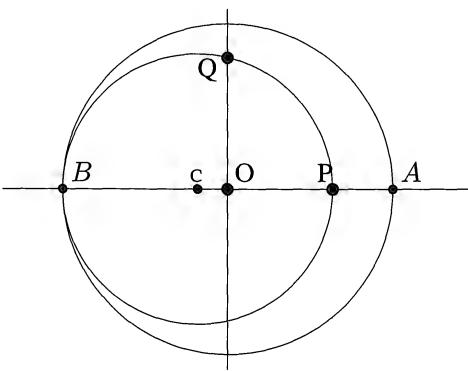
\includegraphics[width=0.42\textwidth]{figs/ch7s3-09.jpg}
\end{center}

如果 $A=(r,0)$ 可构造, 那么 $B=(-r,0)$ 也可构造; $C$ 是线段 $BP$ 的中点 (中点可构造, 见习题~\ref{ex:construct-midpoint}); 以 $C$ 为圆心且经过 $P$ 的圆与正 $y$ 轴相交于一点 $Q=(0,\delta)$, 而初等几何表明 $\delta^2=r$. 因此 $\delta$ 可构造, 这就完成了定理的证明.
\end{proof}

例如, 可以作出一个 $3^{\circ}$ 的角: 据称
\[
\cos 3^{\circ}=\frac{1}{8}(\sqrt{3}+1)\sqrt{5+\sqrt{5}}+\frac{1}{16}(\sqrt{6}-\sqrt{2})(\sqrt{5}-1),
\]
而这个式子表明
\[
\cos 3^{\circ}\in\mathbb{Q}(\sqrt{2},\sqrt{3},\sqrt{5})(\sqrt{5+\sqrt{5}});
\]
也就是说 (由定理~\ref{thm:constructible-quadratic}), $\cos 3^{\circ}$ 可构造. 当然, 一旦作出了 $A=(\cos\theta,0)$, 角 $\theta$ 也就作出了:

\begin{center}
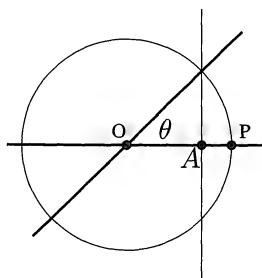
\includegraphics[width=0.42\textwidth]{figs/ch7s3-10.jpg}
\end{center}

下面是定理~\ref{thm:constructible-quadratic} 另一个 ``构造性'' 应用的例子.

\begin{example}\label{ex:pentagon-constructible}
正五边形可构造.

\begin{center}
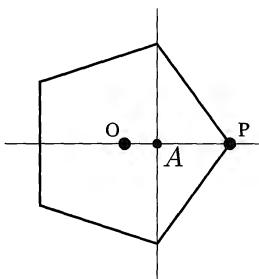
\includegraphics[width=0.42\textwidth]{figs/ch7s3-11.jpg}
\end{center}

确实, 只需作出点 $A=(\cos(2\pi/5),0)$, 而碰巧 $\gamma=\cos(2\pi/5)$ 满足
\begin{equation}
4\gamma^2+2\gamma-1=0.\tag{*}
\end{equation}
\index{huangjinbi@黄金比(golden ratio)}(事实上, $\gamma$ 是黄金分割比倒数的二分之一: $\gamma=\frac{\sqrt{5}-1}{4}$.) 由此可知 $\gamma\in\mathbb{Q}(\sqrt{5})$, 从而由定理~\ref{thm:constructible-quadratic} 它是可构造的. 事实上, 证明展示了如何构造 $\sqrt{5}$, 所以读者现在应当毫不费力地给出正五边形的一个直尺—圆规作图 (习题~\ref{ex:pentagon-construction}).
\end{example}

一旦我们把域论钻研得更透彻一些, 就会回到正多边形的作图问题 (参见 §\ref{subsec:constructible-ngons}). 顺便问一句, 人们是怎么猜到 $\gamma=\cos(2\pi/5)$ 应当满足恒等式 $(*)$ 的? 这借助一点复数运算很容易; 见习题~\ref{ex:verify-pentagon-relation}.

\subsection{著名的不可能性}
\label{subsec:famous-impossibilities}

定理~\ref{thm:constructible-quadratic} 通过下面的直接推论, 轻易地解决了 §\ref{subsec:straightedge-compass} 中提到的三个问题:

\begin{corollary}\label{cor:constructible-degree}
设 $\gamma\in\mathcal{C}_{\mathbb{C}}$ 是一个可构造数. 则 $[\mathbb{Q}(\gamma):\mathbb{Q}]$ 是 $2$ 的幂.
\end{corollary}

\begin{proof}
由引理~\ref{lem:constructible-field} 与定理~\ref{thm:constructible-quadratic}, 存在 $\delta_1,\ldots,\delta_k\in\mathbb{R}$ 使得
\[
\gamma\in\mathbb{Q}(\delta_1,\ldots,\delta_k,i),
\]
并且每个 $\delta_j$ 在 $\mathbb{Q}(\delta_1,\ldots,\delta_{j-1})$ 上的次数 $\leq 2$. 反复应用命题~\ref{prop:tower-degree} 表明
\[
[\mathbb{Q}(\delta_1,\ldots,\delta_k,i):\mathbb{Q}]
\]
是 $2$ 的幂, 而由于
\[
\mathbb{Q}\subseteq\mathbb{Q}(\gamma)\subseteq\mathbb{Q}(\delta_1,\ldots,\delta_k,i),
\]
结论由推论~\ref{cor:degree-divides} 推出.
\end{proof}

特别地, 可构造的实数也必须满足同样的条件.

考虑三等分角的问题. 我们知道可以作出一个 $60^{\circ}$ 的角 (这是作等边三角形的一个副产物). 作出一个 $20^{\circ}$ 的角等价于 (习题~\ref{ex:angle-constructible-cos}) 作出单位圆上辐角为 $\pi/9$ 的复数 $\gamma$:

\begin{center}
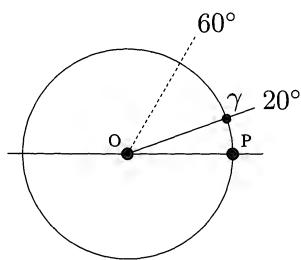
\includegraphics[width=0.42\textwidth]{figs/ch7s3-12.jpg}
\end{center}

现在 $\gamma^9=-1$; 也就是说, $\gamma$ 满足多项式
\[
t^9+1=(t^3+1)(t^6-t^3+1).
\]
它不满足 $t^3+1$; 因此它在 $\mathbb{Q}$ 上的极小多项式是
\[
t^6-t^3+1
\]
的一个因子. 然而, 这个多项式在 $\mathbb{Q}$ 上不可约 (作替换 $t\mapsto t-1$, 然后应用 Eisenstein 判别法), 所以
\[
[\mathbb{Q}(\gamma):\mathbb{Q}]=6.
\]
由推论~\ref{cor:constructible-degree}, $\gamma$ 不可构造. 因此存在可以作出但却不能被三等分的角.

类似地, 立方不能被倍: 因为那将蕴含 $\sqrt[3]{2}$ 的可构造性, 而它在 $\mathbb{Q}$ 上的次数为 $3$, 与推论~\ref{cor:constructible-degree} 矛盾.

化圆为方需要构造 $\sqrt{\pi}$. 但是如果 $\sqrt{\pi}$ 是代数数, 那么 $\pi$ 就会是代数数, 而它不是\erratumfootnote{根据官方勘误, 原书完善了化圆为方不可作的逻辑叙述: 化圆为方需构造 $\sqrt{\pi}$, 若 $\sqrt{\pi}$ 代数则 $\pi$ 代数, 从而导致矛盾 (原书此前曾简略为构造 $\pi$).} (尽管如我们提到过的, 这一事实的证明并不初等), 所以这也是不可能的.

作为另一个例子, 作正七边形相当于构造 $1$ 的一个 $7$ 次 (复) 单位根 $\zeta$:

\begin{center}
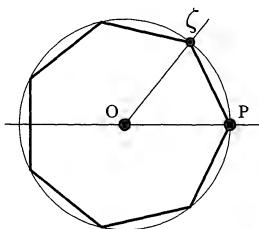
\includegraphics[width=0.42\textwidth]{figs/ch7s3-13.jpg}
\end{center}

依定义, $\zeta$ 满足
\[
t^7-1=(t-1)(t^6+t^5+\cdots+t+1);
\]
由于 $\zeta\neq 1$, $\zeta$ 必须满足分圆多项式 $t^6+\cdots+1$. 它在 $\mathbb{Q}$ 上不可约 (例~V.\ref{ex:cyclotomic-eisenstein}); 因此再次得到 $\zeta$ 在 $\mathbb{Q}$ 上的次数为 $6$, 而推论~\ref{cor:constructible-degree} 蕴含正七边形不能用直尺与圆规作出.

当然 ``$7$'' 并无特别之处: 如果 $p$ 是一个正素数, 则次数为 $p-1$ 的分圆多项式不可约 (还是例~V.\ref{ex:cyclotomic-eisenstein}); 从而
\[
[\mathbb{Q}(\zeta_p):\mathbb{Q}]=p-1,
\]
其中 $\zeta_p$ 是辐角为 $2\pi/p$ 的 $1$ 的复 $p$ 次单位根. 因此, 推论~\ref{cor:constructible-degree} 揭示: 如果 $p$ 是素数, 那么正 $p$ 边形可构造仅当 $p-1$ 是 $2$ 的幂. 这比初看上去限制更强, 因为若 $p=2^k+1$ 是素数, 则必有 $k$ 本身是 $2$ 的幂 (习题~\ref{ex:fermat-prime-power2}). 形如 $2^{2^{\ell}}+1$ 的素数称为 Fermat 素数:
\[
3,\ 5,\ 17,\ 257,\ 65537
\]
(``下一个'', $2^{32}+1=4294967297=641\cdot 6700417$, 不是素数; 事实上, 无人知道是否还有别的 Fermat 素数, 然而有些人猜想有无穷多个).

这些考察本身并不能告诉我们: 如果 $p$ 是 Fermat 素数, 那么正 $p$ 边形就能用直尺与圆规作出; 但它们确实告诉我们, 下一个要考虑的情形将是 $p=2^4+1=17$, 而碰巧 (正如 Gauss 在19岁时所指出的)
\[
\cos\frac{2\pi}{17}=\frac{\sqrt{17}-1+\sqrt{2}\sqrt{34+6\sqrt{17}+\sqrt{2}(\sqrt{17}-1)\sqrt{17-\sqrt{17}}-8\sqrt{2}\sqrt{17+\sqrt{17}}}+\sqrt{2}\sqrt{17-\sqrt{17}}}{16},
\]
因此 (由定理~\ref{thm:constructible-quadratic}) 正十七边形可用直尺与圆规作出. 正如我们已经宣布过的, 情况不久就会变得更加清晰, 使我们能够绕开繁重的三角学.

\subsection*{习题}
\phantomsection
\addcontentsline{toc}{subsection}{习题}

\begin{prob}\label{ex:construct-midpoint}
$\triangleright$ 证明: 若 $A$, $B$ 可构造, 则线段 $AB$ 的中点也可构造. 证明: 若两条直线 $\ell_1$, $\ell_2$ 可构造且不平行, 则平分 $\ell_1$, $\ell_2$ 所成角的两条直线也可构造. [§\ref{subsec:constructible-quadratic}]
\end{prob}

\begin{prob}\label{ex:construct-difference}
$\triangleright$ 证明: 若 $a$, $b$ 是可构造数, 则 $a-b$ 也是. [§\ref{subsec:straightedge-compass}]
\end{prob}

\begin{prob}\label{ex:construct-product}
找出两个实数之积的一个明确的直尺—圆规作图.
\end{prob}

\begin{prob}\label{ex:construct-square-triangle}
证明如何用直尺与圆规把三角形``方化'' (即作一个面积等于给定三角形面积的正方形).
\end{prob}

\begin{prob}\label{ex:lines-circles-over-F}
$\triangleright$ 设 $F$ 是 $\mathbb{R}$ 的一个子域.
\begin{itemize}
\item 设 $A=(x_A,y_A)$, $B=(x_B,y_B)$ 是 $\mathbb{R}^2$ 中两个点, 满足 $x_A,y_A,x_B,y_B\in F$. 证明过 $A$, $B$ 的直线在 $F$ 上定义 (亦即它容许一个系数属于 $F$ 的方程).
\item 证明以 $A$ 为圆心且经过 $B$ 的圆在 $F$ 上定义.
\item 设 $\ell_1$, $\ell_2$ 是 $\mathbb{R}^2$ 中两条不同的, 不平行的直线, 在 $F$ 上定义, 并设 $(x,y)=\ell_1\cap\ell_2$. 证明 $x,y\in F$.
\end{itemize}
[§\ref{subsec:constructible-quadratic}]
\end{prob}

\begin{prob}\label{ex:pentagon-construction}
$\triangleright$ 设计一种用直尺与圆规作正五边形的方法. [§\ref{subsec:constructible-quadratic}]
\end{prob}

\begin{prob}\label{ex:constructible-subfield-C}
$\triangleright$ 把 (实) 平面与 $\mathbb{C}$ 等同, 并把 $O$, $P$ 放在 $\mathbb{C}$ 的 $0$, $1$ 处. 设 $C_{\mathbb{C}}$ 是所有可构造点之集, 视为 $\mathbb{C}$ 的子集. 证明 $C_{\mathbb{C}}$ 是 $\mathbb{C}$ 的一个子域. [§\ref{subsec:straightedge-compass}]
\end{prob}

\begin{prob}\label{ex:constructible-modulus-arg}
设 $\delta\in\mathbb{C}$, $\delta\neq 0$, 并令 $\theta_{\delta}$ 为 $\delta$ 的辐角 (亦即过 $0$ 与 $\delta$ 的直线和实轴所夹的角). 证明 $\delta\in C_{\mathbb{C}}$ 当且仅当 $|\delta|$, $\cos\theta_{\delta}$, $\sin\theta_{\delta}$ 都是可构造实数.
\end{prob}

\begin{prob}\label{ex:complex-quadratic-constructible}
$\triangleright$ 设 $\gamma_1,\ldots,\gamma_k\in\mathcal{C}_{\mathbb{C}}$ 是可构造复数, 并设 $K$ 为域 $\mathbb{Q}(\gamma_1,\ldots,\gamma_k)\subseteq\mathcal{C}_{\mathbb{C}}$. 设 $\delta$ 是一个满足 $[K(\delta):K]=2$ 的复数. 证明 $\delta\in\mathcal{C}_{\mathbb{C}}$.

由此推出: 在 $\mathcal{C}_{\mathbb{C}}$ 上不存在二次的不可约多项式, 并且 $\mathcal{C}_{\mathbb{C}}$ 是具有此性质的最小的 $\mathbb{C}$ 的子域. [§\ref{subsec:constructible-quadratic}]
\end{prob}

\begin{prob}\label{ex:angle-constructible-cos}
$\triangleright$ 证明: 如果在任一可构造构型中两条直线形成一个角 $\theta$, 那么过 $O$ 且相对于直线 $OP$ 顺时针形成角 $\theta$ 的直线可构造.

由此推出: 一个角 $\theta$ 在平面中任何地方可构造, 当且仅当 $\cos\theta$ 可构造. [§\ref{subsec:famous-impossibilities}]
\end{prob}

\begin{prob}\label{ex:verify-pentagon-relation}
$\triangleright$ 验证 $\gamma=\cos(2\pi/5)$ 满足 §\ref{subsec:constructible-quadratic} 中给出的关系 $(*)$. (如果 $\sigma=\sin(2\pi/5)$, 注意 $z=\gamma+i\sigma$ 满足 $z^5-1$.) [§\ref{subsec:constructible-quadratic}]
\end{prob}

\begin{prob}\label{ex:angle-1-2-degree}
证明 $1^{\circ}$ 与 $2^{\circ}$ 的角不可构造. (提示: 根据我们目前所知, 你只需回想存在两个角之和的三角公式; 这些公式的确切形状并不重要.) 对哪些整数 $n$, 角 $n^{\circ}$ 可构造?
\end{prob}

\begin{prob}\label{ex:archimedes-trisection}
$\triangleright$ 证明在下图中 $\alpha=\frac{\theta}{3}$:

\begin{center}
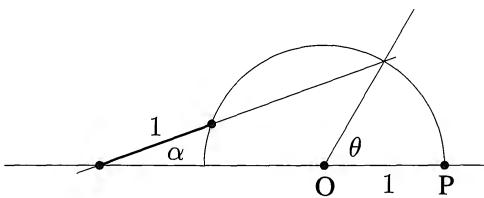
\includegraphics[width=0.42\textwidth]{figs/ch7s3-14.jpg}
\end{center}

这表明: 如果我们允许使用一把 ``标尺'' (亦即一把带标记的直尺), 那么角就可以被三等分 (这里, 这个作图在我们可以在区间上标记一个固定距离 $1$ 时有效). 显然, 这个作图阿基米德已经知道. [§\ref{subsec:straightedge-compass}]
\end{prob}

\begin{prob}\label{ex:nonconstructible-9gon}
证明正九边形不可构造.
\end{prob}

\begin{prob}\label{ex:fermat-prime-power2}
$\triangleright$ 证明: 如果 $2^k+1$ 是素数, 则 $k$ 是 $2$ 的幂. [§\ref{subsec:famous-impossibilities}]
\end{prob}

\section{域扩张, II}\label{sec:field-extensions-2}

是时候继续我们对各类域扩张的巡览了. 这里的关键词是分裂域、正规、可分.

\subsection{分裂域与正规扩张}\label{subsec:splitting-fields}

在 §\ref{subsec:algebraic-closure} 中我们构造了任意给定域 $k$ 的代数闭包 $\overline{k}$: $k[x]$ 中每个多项式都在 $\overline{k}[x]$ 中分裂为一次因式的乘积 (亦即``分裂''), 并且 $\overline{k}$ 是满足此性质的最小的 $k$ 的扩张.

下面是一个类似但温和得多的要求: 给定多项式的一个子集 $\mathcal{F}\subseteq k[x]$, 构造一个扩张 $k\subseteq F$, 使得 $\mathcal{F}$ 中每个多项式都在 $F$ 上分裂为一次因式的乘积, 并且要求 $F$ 在此意义下尽可能小. 此时我们称 $F$ 为 $\mathcal{F}$ 的分裂域. 实际上我们只对 $\mathcal{F}$ 为有限个多项式 $f_1(x),\ldots,f_r(x)$ 的情形感兴趣; 此时要求每个 $f_i(x)$ 在 $F$ 上分裂, 等价于要求乘积 $f_1(x)\cdots f_r(x)$ 在 $F$ 上分裂.

也就是说, 就我们的目的而言, 不妨假设 $\mathcal{F}$ 只由一个多项式 $f(x)\in k[x]$ 组成.

\begin{definition}\label{def:splitting-field}
设 $k$ 是一个域, $f(x)\in k[x]$ 是一个 $d$ 次多项式. $f(x)$ 在 $k$ 上的\emph{分裂域}是一个 $k$ 的扩张 $F$, 使得
\[
f(x)=c\prod_{i=1}^{d}(x-\alpha_i)
\]
在 $F[x]$ 中分裂, 并且进一步 $F=k(\alpha_1,\ldots,\alpha_d)$ 由 $f(x)$ 在 $F$ 中的根在 $k$ 上生成.
\end{definition}

需要注意的是, 分裂域的存在是显然的: 给定 $f(x)\in k[x]$, 子域 $F\subseteq\overline{k}$ (由 $f(x)$ 在 $\overline{k}$ 中的根在 $k$ 上生成) 即满足定义~\ref{def:splitting-field} 的要求. 但我们写定了``the splitting field'' (分裂域), 这是被下面的基本观察的唯一性部分所正当化的; 该观察还估出了这个扩张``有多大''.

\begin{lemma}\label{lem:splitting-field-unique}
设 $k$ 是一个域, $f(x)\in k[x]$. 则 $f(x)$ 在 $k$ 上的分裂域在同构意义下唯一, 并且 $[F:k]\leq(\deg f)!$.

事实上, 若 $\iota:k'\to k$ 是任意域同构, 且 $g(x)\in k'[x]$ 满足 $f(x)=\iota(g(x))$, 则 $\iota$ 可扩张为 $g(x)$ 在 $k'$ 上的任一分裂域到 $f(x)$ 在 $k$ 上的任一分裂域的同构.
\end{lemma}

\begin{proof}
\index{cishu@次数(degree)!bukefen@不可分(inseparable)}我们先显式构造一个分裂域, 并得到陈述中关于次数的界. 然后证明第二部分, 它蕴含在同构意义下的唯一性.

分裂域的构造以及对次数的界, 是我们在命题~V.\ref{prop:adjoin-root} 中得到的基本单扩张的一个简单应用. 归纳地论证: 假设对所有域和所有次数 $\leq(\deg f-1)$ 的多项式, 分裂域都已构造好, 并且界也已证得. 设 $q(t)$ 是 $f(t)$ 在 $k$ 上的任一不可约因子; 则
\[
k\subseteq F':=\frac{k[t]}{(q(t))}
\]
是一个次数为 $\deg q\leq\deg f$ 的扩张, 在其中 $q(x)$ (从而 $f(x)$) 有一个根 (即 $t$ 的陪集 $\alpha$), 因而有一次因子 $x-\alpha$. 多项式 $h(x):=f(x)/(x-\alpha)\in F'[x]$ 的次数为 $(\deg f-1)$; 因此 $h(x)$ 存在一个分裂域 $F$, 并且
\[
[F:F']\leq(\deg f-1)!.
\]
$f(x)$ 在 $F$ 上的因子是 $(x-\alpha)$ 和 $h(x)$ 的因子 (它们都是一次式); 由此推出 $F$ 是 $f(x)$ 的一个分裂域, 并且
\[
[F:k]=[F:F'][F':k]\leq(\deg f)(\deg f-1)!=(\deg f)!
\]
如前所述.

为证明同构 $\iota:k'\to k$ 能如陈述那样扩张为分裂域的同构, 设 $G$ 是 $g(x)$ 的一个分裂域, 并考虑复合 $k'\to k\subseteq\overline{k}$. 由于扩张 $k'\subseteq G$ 是代数的, 由引理~\ref{lem:embed-algebraic-ext} 存在 $G\to\overline{k}$ 的一个保 $k'$ 的扩张同态 $\iota:G\to\overline{k}$. 由于 $G$ 由 $g(x)$ 在 $G$ 中的根在 $k'$ 上生成, 我们有
\[
\iota(G)=k(\alpha_1,\dots,\alpha_d)\subseteq\overline{k},
\]
其中 $\alpha_i$ 是 $f(x)=\iota(g(x))$ 在 $\overline{k}$ 中的根. 因此 $L:=\iota(G)$ 与所选取的同构 $\iota$ 及分裂域 $G$ 无关. 将此观察分别用于给定的 $\iota$ 与恒等同构 $k\to k$, 即得陈述 (因为 $G$ 与 $F$ 都与 $L$ 同构).
\end{proof}

\begin{example}\label{ex:Qi-splitting}
按定义, $\mathbb{Q}(i)$ 是 $x^2+1$ 在 $\mathbb{Q}$ 上的分裂域, 而 $\mathbb{C}$ 是同一多项式在 $\mathbb{R}$ 上的分裂域.
\end{example}

\begin{example}\label{ex:x8-1-splitting}
$x^8-1$ 在 $\mathbb{Q}$ 上的分裂域 $F$ 由 $\zeta:=e^{2\pi i/8}$ 生成: 确实, $x^8-1$ 的根就是 $1$ 的全部 $8$ 次根, 而它们都是 $\zeta$ 的幂.
\begin{center}
\begin{tikzpicture}[scale=1.5]
\draw[gray] (0,0) circle (1);
\draw[gray] (-1.15,0)--(1.7,0);
\draw (0,0)--(45:1);
\draw[dashed,gray] (0,0)--(-45:1)--({sqrt(2)},0)--(45:1);
\foreach \a in {0,45,...,315} {\fill (\a:1) circle (1.3pt);}
\fill (0,0) circle (2pt) node[above left] {$0$};
\fill (1,0) circle (2pt) node[above right] {$1$};
\fill (45:1) circle (2pt) node[above] {$\zeta$};
\fill (0,1) circle (2pt) node[above] {$i$};
\fill ({sqrt(2)},0) circle (1.5pt) node[below] {$\sqrt2$};
\end{tikzpicture}
\end{center}


实际上, $\zeta$ 是多项式 $x^4+1$ 的根, 而该多项式在 $\mathbb{Q}$ 上不可约; 因此 $F=\mathbb{Q}(\zeta)$ ``已经''是 $x^4+1$ 的分裂域. $F$ 在 $\mathbb{Q}$ 上的次数为
\[
[\mathbb{Q}(\zeta):\mathbb{Q}]=4,
\]
远小于引理~\ref{lem:splitting-field-unique} 给出的界 $8!$, $4!$.

为了更好理解这个分裂域, 注意到 $i=\zeta^2$ 属于 $F$, 并且 $\sqrt{2}=\zeta+\zeta^7$ 也属于 $F$; 于是 $F$ 包含 $\mathbb{Q}(i,\sqrt{2})$. 反过来, $\zeta=\frac{\sqrt{2}}{2}(1+i)\in\mathbb{Q}(i,\sqrt{2})$. 因此 $x^4+1$ 的分裂域 (亦即 $x^8-1$ 的分裂域) 就是 $\mathbb{Q}(i,\sqrt{2})$. 像我们在例~\ref{ex:sqrt2-sqrt3} 中对扩张 $\mathbb{Q}\subseteq\mathbb{Q}(i,\sqrt{2})$ 所做的那样分析, 可知其关于 $\mathbb{Q}$ 的自同构群是 $\mathbb{Z}/2\mathbb{Z}\times\mathbb{Z}/2\mathbb{Z}$.
\end{example}

\begin{example}\label{ex:x4-1-splitting}
主题的一个变体: $x^4-1$. 如果考虑的不是 $x^4+1$ 而是 $x^4-1$, 情形就不同了: 该多项式在 $\mathbb{Q}$ 上分解,
\[
x^4-1=(x-1)(x+1)(x^2+1),
\]
由此可知其分裂域与 $x^2+1$ 的分裂域相同, 即就是 $\mathbb{Q}(i)$.
\end{example}

\begin{example}\label{ex:x4+2-splitting}
主题的一个变体: $x^4+2$. 过于乐观的读者此刻或许期望, $x^4+1$ 与 $x^4-1$ 在 $\mathbb{Q}$ 上分裂域的不同, 仅仅源于前者在 $\mathbb{Q}$ 上不可约而后者可约. 这个例子会让任何这样的猜测胎死腹中. 沿用例~\ref{ex:x8-1-splitting} 的记号, $x^4+2$ 的根是
\[
\sqrt[4]{2}\,\zeta,\ \sqrt[4]{2}\,\zeta^3,\ \sqrt[4]{2}\,\zeta^5,\ \sqrt[4]{2}\,\zeta^7.
\]
因此, 以 $K=\mathbb{Q}(\sqrt[4]{2}\zeta,\sqrt[4]{2}\zeta^3,\sqrt[4]{2}\zeta^5,\sqrt[4]{2}\zeta^7)$ 记 $x^4+2$ 的分裂域, 有
\[
K\subseteq\mathbb{Q}(\zeta,\sqrt[4]{2})=\mathbb{Q}(i,\sqrt{2},\sqrt[4]{2})=\mathbb{Q}(i,\sqrt[4]{2}).
\]
另一方面, $\sqrt{2}=(\sqrt[4]{2}\zeta)^3/(\sqrt[4]{2}\zeta^3)\in K$; 从而 $i=(\sqrt[4]{2}\zeta)^2/\sqrt{2}\in K$; 从而 $\zeta=\frac{\sqrt{2}}{2}(1+i)\in K$; 从而 $\sqrt[4]{2}=(\sqrt[4]{2}\zeta)/\zeta\in K$. 于是 $\mathbb{Q}(i,\sqrt[4]{2})\subseteq K$, 结论便是 $x^4+2$ 的分裂域等于 $K=\mathbb{Q}(i,\sqrt[4]{2})$. 一个简单的次数计算 (习题~\ref{ex:aut-group-x4+2}) 表明 $[K:\mathbb{Q}]=8$, 特别地 $x^4+2$ 的分裂域当然不同构于 $x^4+1$ 的分裂域\erratumfootnote{根据官方勘误, 原书在此处完善了生成元包含关系的推理步骤与分裂域次数计算结论.}.

\index{duoxiangshi@多项式(polynomial)!zai UFD shangbukeyue@在 UFD 上不可约(irreducible over a UFD)}这样的例子总让我觉得域论必定相当神秘: 问题参数的看似无害的变化, 可能引起相应域扩张剧烈的改变. 从正面说, 这暗示域论确实是 (例如) 多项式研究中一件非常精确的工具.
\end{example}

\index{duoxiangshi@多项式(polynomial)!Laurent@Laurent}分裂域在后续故事中扮演着重要角色. 它们比初看起来还要特殊: 不仅分裂所给的多项式, 而且自动分裂任何``胆敢用一个根触碰它们''的不可约多项式. 这使分裂域成为正规扩张:

\begin{definition}\label{def:normal-extension}
一个域扩张 $k\subseteq F$ 是\emph{正规的}, 如果对每个不可约多项式 $f(x)\in k[x]$, $f(x)$ 在 $F$ 中有一个根当且仅当 $f(x)$ 在 $F$ 上分裂为一次因式的乘积.
\end{definition}

\begin{theorem}\label{thm:finite-normal-splitting}
一个域扩张 $k\subseteq F$ 是有限且正规的, 当且仅当 $F$ 是某个多项式 $f(x)\in k[x]$ 的分裂域.
\end{theorem}

\begin{proof}
假设 $k\subseteq F$ 有限且正规. 则 $F$ 有限生成: $F=k(\alpha_1,\ldots,\alpha_r)$, 其中每个 $\alpha_i$ 在 $k$ 上代数. 设 $p_i(x)$ 是 $\alpha_i$ 在 $k$ 上的极小多项式\erratumfootnote{根据官方勘误, 此处多项式不定元由 $t$ 统一记为 $x$ ($p_i(x)$ 与 $f(x)$).}. 由于 $F$ 在 $k$ 上正规, 每个 $p_i(x)$ 在 $F$ 上完全分裂, 从而 $f(x)=p_1(x)\cdots p_r(x)$ 也如此. 由此可知 $F$ 是 $f(x)$ 的分裂域.

反过来, 假设 $F$ 是某个多项式 $f(x)\in k[x]$ 的分裂域, 并设 $p(x)\in k[x]$ 是一个不可约多项式, 使得 $F$ 包含 $p(x)$ 的一个根 $\alpha$. 将 $F$ 视为代数闭包 $\overline{k}$ 的子域, 设 $\beta\in\overline{k}$ 是 $p(x)$ 的任一其他根; 我们将证明 $\beta\in F$. 这就证明了 $F$ 包含 $p(x)$ 的所有根, 从而 $k\subseteq F$ 正规, 并且由引理~\ref{lem:splitting-field-unique} 知 $k\subseteq F$ 有限.

由命题~\ref{prop:simple-ext-iso-lift}, 存在同构 $\iota:k(\alpha)\to k(\beta)$ 保 $k$ 上的恒等并将 $\alpha\mapsto\beta$. 我们还考虑子域 $F(\beta)\subseteq\overline{k}$, 视其为 $k(\beta)$ 的扩张. 把一切都放进一个图:

\begin{center}
\begin{tikzcd}[column sep=2.5em,row sep=1.4em]
& k(\alpha) \ar[dd,"\iota"] \ar[r,hook] & F \ar[r,hook] & \overline{k} \\
k \ar[ur,hook] \ar[dr,hook] & & & \\
& k(\beta) \ar[r,hook] & F(\beta) \ar[r,hook] & \overline{k}
\end{tikzcd}
\end{center}

(注意: 如果我们用恒等映射把右边的两个 $\overline{k}$ 连接起来, 相应的图并不交换: $\iota$ 把上行中的 $\alpha\in\overline{k}$ 送到下行中的 $\beta\in\overline{k}$.) 现在观察到, $F$ 可视为 $f(x)$ 在 $k(\alpha)$ 上的分裂域: 确实, 它包含 $f(x)$ 的所有根, 并且由这些根在 $k$ 上 (从而在 $k(\alpha)$ 上) 生成. 同理, $F(\beta)$ 是 $f(x)$ 在 $k(\beta)$ 上的分裂域. 由引理~\ref{lem:splitting-field-unique}, $\iota$ 可扩张为同构 $\iota':F\to F(\beta)$. 由于 $\iota$ 在 $k$ 上限制为恒等, $\iota'$ 是 $k$-向量空间的同构; 特别地, $\dim_k F=\dim_k F(\beta)$ (记住分裂域都是有限扩张).

现在考虑不同的 $k$-线性映射 $i:F\to F(\beta)$, 它简单地由在 $\overline{k}$ 中的包含给出:
\[
k\subseteq F\subseteq F(\beta)\subseteq\overline{k}.
\]
由于 $F$ 与 $F(\beta)$ 是同维数的有限维 $k$-向量空间, $i$ 也必须是同构. 换言之,
\[
[F(\beta):F]=1;
\]
即 $\beta\in F$, 如所求.
\end{proof}

\begin{remark}\label{rmk:normal-proof}
这个论证有点精巧. 沿用证明中的记号, 图
\begin{center}
\begin{tikzcd}[column sep=large,row sep=large]
k(\alpha) \ar[r,hook] \ar[d,"\iota"'] & F \ar[d,"\iota'"] \\
k(\beta) \ar[r,hook] & F(\beta)
\end{tikzcd}
\end{center}
是交换的, 而图
\begin{center}
\begin{tikzcd}[column sep=large,row sep=large]
k(\alpha) \ar[r,hook] \ar[d,"\iota"'] & F \ar[d,"i"] \\
k(\beta) \ar[r,hook] & F(\beta)
\end{tikzcd}
\end{center}
在 $\beta\neq\alpha$ 时不交换. 确实, $\iota$ 把 $\alpha$ 送到 $\beta$, 而 $i$ 把 $\alpha$ 送到 $\alpha$. 论证的要点是观察到: 若存在两个有限维向量空间 $V$, $W$ 之间的一个同构, 则每个单射线性映射 $V\to W$ 都必须是同构. 有限维性是得出结论所必需的; 参见习题~VI.\ref{ex:k[t]-injective-not-surjective}.
\end{remark}

\begin{example}\label{ex:normal-Qi-root4}
如果一个不可约多项式 $p(x)\in\mathbb{Q}[x]$ 的一个复根可以表示为 $i$ 与 $\sqrt[4]{2}$ 的带有理系数的多项式, 那么 $p(x)$ 的所有根也都可以同样用 $i$ 与 $\sqrt[4]{2}$ 表示. 确实, 我们已经验证 (例~\ref{ex:x4+2-splitting}) $\mathbb{Q}(i,\sqrt[4]{2})$ 是 $\mathbb{Q}$ 上的分裂域; 从而它是 $\mathbb{Q}$ 的正规扩张.
\end{example}

\subsection{可分多项式}\label{subsec:separable-polynomials}

我们的直觉或许会引导我们认为, 如果一个多项式分解为一次因式的乘积, 并且我们不是``故意''重复其中一个因子 (如 $(x-1)^2(x-2)$ 那样), 那么这些因子就会互异. 例如, 不可约多项式在代数闭包中分裂时, 其因子必然互异, 对吧? 错了.

\begin{example}\label{ex:xp-t-insep}
设 $p$ 是素数, 考虑 $\mathbb{F}_p$ 上的有理函数域 $\mathbb{F}_p(t)$. 则多项式
\[
x^p-t\in\mathbb{F}_p(t)[x]
\]
不可约: 由 Eisenstein 判别法它在 $\mathbb{F}_p[t][x]$ 中不可约 (因为 $(t)$ 在 $\mathbb{F}_p[t]$ 中是素理想), 从而由命题~V.\ref{prop:irreducible-over-field} 在 $\mathbb{F}_p(t)[x]$ 中不可约. 设 $u$ 是该多项式在某个 $L\supseteq\mathbb{F}_p(t)$ 中的根 (例如 $L$ 可以取 $\mathbb{F}_p(t)$ 的代数闭包, 或更温和地取该多项式的一个分裂域). 则 (习题~\ref{ex:frobenius-add})
\[
x^p-t=(x-u)^p
\]
在 $L[x]$ 中; 也就是说, $u$ 作为 $f(x)$ 的根具有重数 $p$.

换句话说, $u\in L$ 在 $\mathbb{F}_p(t)$ 上的极小多项式在 $u$ 处 $p$ 重为零, 对此我们无能为力: 没有比 $(x-u)^p=x^p-t$ 次数更小的 $(x-u)$ 的幂其系数落在 $\mathbb{F}_p(t)$ 中 (更小的幂会给出 $x^p-t$ 的一个非平凡因子, 而 $x^p-t$ 不可约).

我们一直觉得这个例子难以想象, 因为在特征 $0$ 中培养出的直觉; 并且如我们将看到的, 在特征 $0$ 中不可能出现这样的病态.
\end{example}

\begin{definition}\label{def:separable-poly}
设 $k$ 是一个域. 一个多项式 $f(x)\in k[x]$ 是\emph{可分的}, 如果它在自己的分裂域上没有重因子; $f(x)$ 是\emph{不可分的}, 如果它在自己的分裂域上有重因子.
\end{definition}

于是例~\ref{ex:xp-t-insep} 中的多项式 $x^p-t$ 是不可分的. 我们猜想这个术语反映了我们无法``分离''它的根: 它们像质子中的夸克一样抱成一团, 我们无法把它们拆开.

当然定义~\ref{def:separable-poly} 不依赖于所选取的分裂域, 因为这些分裂域在同构意义下唯一 (引理~\ref{lem:splitting-field-unique}). 事实上, 为了检测可分性, 我们可以使用任何一个使该多项式分裂为一次因式的域 (由习题~\ref{ex:splitting-field-hom}). 关于可分性的第一个 (有点令人惊讶的) 观察是, 我们其实不必离开 $f(x)$ 的系数域就能检测它. 这个事实用到了从微积分借来的一个概念: 对多项式
\[
f(x)=a_0+a_1x+a_2x^2+\dots+a_nx^n,
\]
我们以
\[
f'(x)=a_1+2a_2x+\dots+na_nx^{n-1}
\]
记其``导数''.

当然这是一个纯形式的运算; 在任意域上都不涉及极限过程. 尽管如此, 导数的一切预期性质都成立, 读者应当验证: 例如通常有 $(fg)'=f'g+fg'$.

\begin{lemma}\label{lem:separable-gcd}
设 $k$ 是一个域, $f(x)\in k[x]$. 则 $f(x)$ 可分当且仅当 $f(x)$ 与 $f'(x)$ 互素.
\end{lemma}

按定义, $f(x)$ 与 $f'(x)$ 互素恰好是它们的最大公因式为 $1$. 注意若 $k\subseteq F$, 则 $f(x)$ 与 $f'(x)$ 的最大公因式在 $k[x]$ 中与在 $F[x]$ 中是相同的: 例如因为它可以通过 Euclid 算法 (§V.\ref{subsec:euclidean-pid}) 计算, 而无论在计算在 $k[x]$ 中还是 $F[x]$ 中进行, 过程都完全一样.

\begin{proof}
先假设 $f(x)$ 不可分. 则 $f(x)$ 在某个分裂域 $F$ 中有重根; 即
\[
f(x)=(x-\alpha)^mg(x)
\]
对某个 $\alpha\in F$, $g(x)\in F[x]$, 且 $m\geq 2$. 于是
\[
f'(x)=m(x-\alpha)^{m-1}g(x)+(x-\alpha)^mg'(x),
\]
从而 $(x-\alpha)$ 是 $f(x)$ 与 $f'(x)$ 在 $F[x]$ 中的一个公因子. 因此 $\gcd(f(x),f'(x))\neq 1$ 在 $F[x]$ 中; 从而 $\gcd(f(x),f'(x))\neq 1$ 在 $k[x]$ 中; 即 $f(x)$, $f'(x)$ 不互素.

反过来, 假设 $\gcd(f(x),f'(x))\neq 1$, 于是 $f(x)$ 与 $f'(x)$ 在 $k$ 的代数闭包 $\overline{k}$ 中有一个公共的不可约因子 $(x-\alpha)$. 写 $f(x)=(x-\alpha)h(x)$; 我们有
\[
f'(x)=h(x)+(x-\alpha)h'(x),
\]
从而 $x-\alpha$ 整除 $h(x)$, 因为它整除 $f'(x)$. 但于是
\[
(x-\alpha)^2\mid f(x);
\]
故 $f(x)$ 不可分.
\end{proof}

例如, 例~\ref{ex:xp-t-insep} 中的多项式 $x^p-t$ 无须借助分裂域即可看出不可分: 在特征 $p$ 中 $x^p-t$ 的导数等于 $px^{p-1}=0$, 而 $\gcd(x^p-t,0)=x^p-t\neq 1$.

\index{bukefen@不可分(inseparable)}这个例子抓住了不可分性的一个关键特征:

\index{bukefen@不可分(inseparable)!chun@纯(purely)}\index{bukefen@不可分(inseparable)!duoxiangshi@多项式(polynomial)}\index{bukefen@不可分(inseparable)!kuozhangdeyuan@扩张的元(element of an extension)}\index{bukefen@不可分(inseparable)!cishu@次数(degree)}\begin{lemma}\label{lem:inseparable-deriv-zero}
设 $k$ 是一个域, $f(x)\in k[x]$ 是一个不可分的不可约多项式. 则 $f'(x)=0$.
\end{lemma}

\begin{proof}
由于 $f(x)$ 不可分, 由引理~\ref{lem:separable-gcd} 知 $f(x)$ 与 $f'(x)$ 有一个公共的不可约因子 $q(x)$; 但 $f(x)$ 自身不可约, 故 $q(x)$ 必与 $f(x)$ 相伴, 并且特别地其次数大于 $f'(x)$ 的次数 (若 $f'(x)\neq 0$). 由于 $q(x)\mid f'(x)$, 唯一的可能就是 $f'(x)=0$.
\end{proof}

\index{duoxiangshidedaoshu@多项式的导数(derivative of a polynomial)}这已经告诉我们, 不可约多项式在特征 $0$ 中必然可分: 在特征 $0$ 中, 一个非常数多项式的导数显然不可能为零. 事实上, 引理~\ref{lem:inseparable-deriv-zero} 给我们一幅关于不可分的不可约多项式必然形如怎样的精确图画. 如果
\[
f(x)=\sum_{i=0}^{n}a_ix^i
\]
不可约且不可分, 则域的特征必为正素数 $p$, 并且由引理~\ref{lem:inseparable-deriv-zero} 必有
\[
f'(x)=\sum_{i=0}^{n}ia_ix^{i-1}=0;
\]
即对所有 $i$ 有 $ia_i=0$. 现在若 $i$ 是 $p$ 的倍数, 则 $ia_i=0$ 自动成立; 而它对一切不是 $p$ 的倍数的指标 $i$ 推出 $a_i=0$. 因此 $f(x)$ 中唯一可能非零的系数, 是那些对应于 $p$ 的倍数指标的:
\[
f(x)=a_0+a_px^p+a_{2p}x^{2p}+\ldots;
\]
于是 $f(x)$ 实际上必须是一个 $x^p$ 的多项式. (读者将通过完成习题~\ref{ex:inseparable-degree} 及其后续而进一步细化这幅图画.)

这引导我们得到一个把可分性与我们尚未遇到的一类域联系起来的精确结果.

\begin{definition}\label{def:frobenius}
设 $k$ 是特征 $p>0$ 的域. \emph{Frobenius 同态}是映射 $k\to k$, 定义为 $x\mapsto x^p$.
\end{definition}

Frobenius 同态乍看不像一个环同态, 但它确实是 (习题~\ref{ex:frobenius-add}). 它必然单射, 正如每个非平凡的域同态那样; 但它未必满射.

\begin{definition}\label{def:perfect}
一个域 $k$ 是\emph{完全的}, 如果 $\Char k=0$, 或者 $\Char k>0$ 且 Frobenius 同态是满射.
\end{definition}

\begin{proposition}\label{prop:perfect-sep}
设 $k$ 是一个域. 则 $k$ 是完全的当且仅当 $k[x]$ 中所有不可约多项式都可分.
\end{proposition}

\begin{proof}
我们将证明完全域上的不可约多项式可分, 把另一个方向留给读者 (习题~\ref{ex:not-perfect-insep}).

我们已经注意到, 特征为零的域上的不可约多项式可分. 在正特征 $p$ 中, 我们观察到, 一个不可分的不可约多项式必形如
\[
f(x)=\sum_{i=0}^{m}a_i\cdot(x^p)^i.
\]
由于 Frobenius 是满射, 存在 $b_i$ 使得 $b_i^p=a_i$. 于是
\[
f(x)=\sum_{i=0}^{m}b_i^p(x^p)^i=\sum_{i=0}^{m}(b_ix^i)^p=\left(\sum_{i=0}^{m}b_ix^i\right)^p=g(x)^p,
\]
其中 $g(x)=\sum b_ix^i$, 并记住 Frobenius 映射是一个同态. 但这与 $f(x)$ 的不可约性矛盾, 故不存在这样的多项式.
\end{proof}

\begin{corollary}\label{cor:finite-fields-perfect}
\index{youxianyu@有限域(finite field)}有限域是完全的. 从而, 在有限域上, 不可约多项式都可分.
\end{corollary}

\begin{proof}
Frobenius 映射是单射 (因为它是域的同态), 从而在有限域上由鸽笼原理它是满射. 因此有限域是完全的, 而陈述的第二部分由命题~\ref{prop:perfect-sep} 推出. \qed
\end{proof}

读者现在明白我们为何在例~\ref{ex:xp-t-insep} 中选择那个有点不寻常的域 $\mathbb{F}_p(t)$ 了: 我们需要一个正特征的域, 但是在 $F_p$ 上由推论~\ref{cor:finite-fields-perfect} 找不到任何不可分的不可约多项式的例子; 为了构造一个例子, 我们必须放大这个域使其无限, 并且塞进一个元素 (即 $t$), 它对它没有 $p$ 次根, 亦即不在 Frobenius 的像中.

\subsection{可分扩张与在代数闭包中的嵌入}\label{subsec:separable-extensions-embeddings}

上一小节考察的术语可以推广到域扩张的语言中. 如果 $k\subseteq F$ 是一个扩张且 $\alpha\in F$ 在 $k$ 上代数, 我们说 $\alpha$ 在 $k$ 上\emph{可分}, 如果 $\alpha$ 在 $k$ 上的极小多项式可分; 否则 $\alpha$ \emph{不可分}.

\begin{definition}\label{def:separable-extension}
一个代数域扩张 $k\subseteq F$ 是\emph{可分的}, 如果每个 $\alpha\in F$ 都在 $k$ 上可分.
\end{definition}

用这个术语, 命题~\ref{prop:perfect-sep} 可以重述为以下更唬人的形式:

\begin{proposition}\label{prop:perfect-sep-ext}
一个域 $k$ 是完全的, 当且仅当 $k$ 的每个代数扩张都可分.
\end{proposition}

特别地, $\mathbb{Q}$ (或任意特征为零的域) 的代数扩张, 以及每个有限域的代数扩张, 必然可分.

可分性条件极其方便, 并且我们此后实质上采用它: 我们将认真考虑的所有扩张都是可分的. 可分扩张的一个方便的特性, 是以下对可分性条件的另一种刻画.

我们已经看到 (引理~\ref{lem:embed-algebraic-ext}) 每个代数扩张 $k\subseteq F$ 都可嵌入一个代数闭包 $k\subseteq\overline{k}$, 并且我们指出这一般可以用许多不同的方式做到. 如果是有限的, 把 $F\to\overline{k}$ 中保 $k$ 上恒等的不同同态的个数记为
\[
[F:k]_s.
\]

\begin{definition}\label{def:separable-degree}
这就是 $F$ 在 $k$ 上的\emph{可分次数}.
\end{definition}

显然这个数与所选取的代数闭包 $k\subseteq\overline{k}$ 无关. 它与可分性有什么关系呢?

\begin{lemma}\label{lem:simple-sep-degree}
设 $k\subseteq k(\alpha)$ 是一个单代数扩张. 则 $[k(\alpha):k]_s$ 等于 $\alpha$ 的极小多项式在 $\overline{k}$ 中不同根的个数. 特别地, $[k(\alpha):k]_s\leq[k(\alpha):k]$, 并且等号成立当且仅当 $\alpha$ 在 $k$ 上可分.
\end{lemma}

\begin{proof}
证明实质上是 (并且不是巧合地) 推论~\ref{cor:autk-count} 证明的重述. 把每个保 $\mathrm{id}_k$ 的 $\iota:k(\alpha)\to\overline{k}$ 与其像 $\iota(\alpha)$ 对应, 后者必是 $\alpha$ 的极小多项式的根. 这个对应是单射, 因为 $\iota(\alpha)$ 决定了 $\iota$ (由于 $\iota$ 扩充 $k$ 上的恒等). 为见其满射, 设 $\beta\in\overline{k}$ 是任一其他根, 并考虑扩张 $k(\beta)\subseteq\overline{k}$; 由命题~\ref{prop:simple-ext-iso-lift} 存在同构 $k(\alpha)\to k(\beta)$ 把 $\alpha$ 送到 $\beta$, 再与嵌入 $k(\beta)\subseteq\overline{k}$ 复合即定义出相应的 $\iota$, 如所求.
\end{proof}

\index{cishu@次数(degree)!kefen@可分(separable)}于是, 对单扩张而言, ``可分次数''确实检测可分性. 进一步, 它对连续扩张是乘法的:

\begin{lemma}\label{lem:sep-degree-tower}
设 $k\subseteq E\subseteq F$ 是代数扩张. 则 $[F:k]_s$ 有限当且仅当 $[F:E]_s$, $[E:k]_s$ 都有限, 并且此时
\[
[F:k]_s=[F:E]_s[E:k]_s.
\]
\end{lemma}

\begin{proof}
$E$ 到 $\overline{k}$ 的不同嵌入的不同延拓, 由引理~\ref{lem:embed-algebraic-ext} 给出 $F$ 到 $\overline{k}$ 的不同嵌入; 而 $F$ 到 $\overline{E}=\overline{k}$ 中保 $E$ 上恒等的嵌入, 当然也保 $k$ 上的恒等. 因此, 若 $[F:E]_s$, $[E:k]_s$ 中有一个无限, 则 $[F:k]_s$ 也无限.

对反向蕴含, 只需证明所陈述的次数公式. 但每个保 $k$ 上恒等的嵌入 $F\subseteq\overline{k}$ 都可由两步得到: 先把恒等扩张为嵌入 $E\subseteq\overline{k}$, 这有 $[E:k]_s$ 种做法; 再把所选取的嵌入 $E\subseteq\overline{k}=\overline{E}$ 扩张为嵌入 $F\subseteq\overline{E}=\overline{k}$, 这有 $[F:E]_s$ 种做法. 恰好有 $[F:E]_s[E:k]_s$ 种做法, 如陈述.
\end{proof}

引理~\ref{lem:simple-sep-degree} 与引理~\ref{lem:sep-degree-tower} 使我们能把有限扩张的可分性完全用代数闭包中嵌入的计数来重述:

\begin{proposition}\label{prop:finite-sep-degree}
设 $k\subseteq F$ 是一个有限扩张. 则 $[F:k]_s\leq[F:k]$, 并且以下等价:

(i) $F=k(\alpha_1,\ldots,\alpha_r)$, 其中每个 $\alpha_i$ 在 $k$ 上可分;

(ii) $k\subseteq F$ 可分;

(iii) $[F:k]_s=[F:k]$.
\end{proposition}

\begin{proof}
由于 $F$ 在 $k$ 上有限, 它有限生成. 设 $F=k(\alpha_1,\ldots,\alpha_r)$. 则利用引理~\ref{lem:sep-degree-tower}, 引理~\ref{lem:simple-sep-degree}, 以及命题~\ref{prop:tower-degree},
\[
\begin{array}{r l}
[F:k]_s & =[k(\alpha_1,\ldots,\alpha_{r-1})(\alpha_r):k(\alpha_1,\ldots,\alpha_{r-1})]_s\cdots[k(\alpha_1):k]_s \\
& \leq [k(\alpha_1,\ldots,\alpha_{r-1})(\alpha_r):k(\alpha_1,\ldots,\alpha_{r-1})]\cdots[k(\alpha_1):k] \\
& =[F:k].
\end{array}
\]
这证明了所陈述的不等式.

(i)$\Longrightarrow$(iii): 若每个 $\alpha_i$ 在 $k$ 上可分, 则它在域 $k(\alpha_1,\ldots,\alpha_{i-1})$ 上也可分 (习题~\ref{ex:separable-over-intermediate}), 故由引理~\ref{lem:simple-sep-degree} 不等式取等号.

(iii)$\Longrightarrow$(ii): 假设 $[F:k]_s=[F:k]$, 并设 $\alpha\in F$. 我们有 $k\subseteq k(\alpha)\subseteq F$; 从而由引理~\ref{lem:sep-degree-tower}
\[
[F:k(\alpha)]_s[k(\alpha):k]_s=[F:k]_s=[F:k]=[F:k(\alpha)][k(\alpha):k].
\]
\index{fenci@分次(graded)}由于两个可分次数都小于等于各自的普通次数, 这个等式推出
\[
[k(\alpha):k]_s=[k(\alpha):k],
\]
由引理~\ref{lem:simple-sep-degree} 即证 $\alpha$ 可分. 因此扩张 $k\subseteq F$ 按定义~\ref{def:separable-extension} 可分.

(ii)$\Longrightarrow$(i) 由定义~\ref{def:separable-extension} 立得, 因为有限扩张有限生成.
\end{proof}

例如, 若 $\alpha$ 在 $k$ 上可分, 则每个 $\beta\in k(\alpha)$ 都可分. 这单从定义看会显得相当神秘: 为什么 $\alpha$ 的极小多项式在 $\overline{k}$ 中有互异的根, 就能推出 $\beta$ 的极小多项式也如此? 它确实能, 凭借命题~\ref{prop:finite-sep-degree}.

\begin{remark}\label{rmk:sep-degree-divides}
虽然我们只证明了 $[F:k]_s\leq[F:k]$, 其实还可以证明 $[F:k]_s$ 整除 $[F:k]$: 事实上, $[F:k]_s$ 是某个中间域 $F_{\mathrm{sep}}$ 在 $k$ 上的次数. 勤勉的读者将在习题~\ref{ex:inseparable-degree-props} 中证明这一点.\index[sym1]{17@$F_{\mathrm{sep}}$}
\end{remark}

\subsection*{习题}
\phantomsection
\addcontentsline{toc}{subsection}{习题}

\begin{prob}\label{ex:splitting-field-hom}
$\triangleright$ 设 $k$ 是域, $f(x)\in k[x]$, 并设 $F$ 是 $f(x)$ 在 $k$ 上的分裂域. 设 $k\subseteq K$ 是一个扩张, 使得 $f(x)$ 在 $K$ 上分裂为一次因式的乘积. 证明存在同态 $F\to K$ 保 $k$ 上的恒等. [§\ref{subsec:splitting-fields}]
\end{prob}

\begin{prob}\label{ex:splitting-x6+x3+1}
描述 $x^6+x^3+1$ 在 $\mathbb{Q}$ 上的分裂域. 对 $x^4+4$ 做同样的事.
\end{prob}

\begin{prob}\label{ex:aut-group-x4+2}
$\triangleright$ 求 $x^4+2$ 在 $\mathbb{Q}$ 上的分裂域的自同构群的阶 (参见例~\ref{ex:x4+2-splitting})\erratumfootnote{根据官方勘误, 此题编号与对应的例交叉引用核对一致 (cf. Example 4.6).}. [§\ref{subsec:splitting-fields}]
\end{prob}

\begin{prob}\label{ex:Q-root4-not-splitting}
证明域 $\mathbb{Q}(\sqrt[4]{2})$ 不是任何 $\mathbb{Q}$ 上多项式的分裂域.
\end{prob}

\begin{prob}\label{ex:splitting-of-factor}
$\triangleright$ 设 $F$ 是多项式 $f(x)\in k[x]$ 的一个分裂域, 并设 $g(x)\in k[x]$ 是 $f(x)$ 的一个因子. 证明存在唯一的中间域 $k\subseteq G\subseteq F$ 使得 $k\subseteq G$ 是 $g(x)$ 的分裂域\erratumfootnote{根据官方勘误, 原题陈述严密化为: ``存在唯一的中间域 $k\subseteq G\subseteq F$ 使得 $k\subseteq G$ 是 $g(x)$ 的分裂域 (there is a unique intermediate field $k\subseteq G\subseteq F$ such that $k\subseteq G$ is a splitting field for $g(x)$)''.}. [\S\ref{subsec:finite-fields}]
\end{prob}

\begin{prob}\label{ex:intersection-composite-splitting}
设 $k\subseteq F_1$, $k\subseteq F_2$ 是两个有限扩张, 视为嵌入 $k$ 的代数闭包 $\overline{k}$ 中. 假设 $F_1$ 与 $F_2$ 都是 $k[x]$ 中多项式的分裂域. 证明交 $F_1\cap F_2$ 与复合 $F_1F_2$ ($\overline{k}$ 中包含 $F_1$ 与 $F_2$ 的最小子域) 也都是 $k$ 上的分裂域. (定理~\ref{thm:finite-normal-splitting} 大概会有帮助.)
\end{prob}

\begin{prob}\label{ex:simple-normal-aut}
$\triangleright$ 设 $k\subseteq F=k(\alpha)$ 是一个单代数扩张. 证明 $F$ 在 $k$ 上正规, 当且仅当对每个代数扩张 $F\subseteq K$ 和每个 $\sigma\in\Aut_k(K)$, 都有 $\sigma(F)=F$. [\S\ref{subsec:galois-correspondence}]
\end{prob}

\begin{prob}\label{ex:frobenius-add}
$\triangleright$ 设 $p$ 是素数, $k$ 是特征 $p>0$ 的域. 对 $a,b\in k$\erratumfootnote{根据官方勘误, 特征明确标明为 $p>0$, 元素所属域由大写 $K$ 修正为小写 $k$ ($a,b\in k$).}, 证明\footnote{这就是所谓``菜鸟之梦''; 它在任意特征 $p$ 的交换环中都成立, 由二项式定理以及中间二项式系数 $\binom{p}{k}$ 对 $0<k<p$ 均被 $p$ 整除.} $(a+b)^p=a^p+b^p$. [§\ref{subsec:separable-polynomials}, §\ref{subsec:finite-fields}, §\ref{subsec:cyclotomic}]
\end{prob}

\begin{prob}\label{ex:derivative-product}
利用 §\ref{subsec:separable-polynomials} 中给出的``导数''概念, 证明对所有多项式 $f$, $g$ 有 $(fg)'=f'g+fg'$.
\end{prob}

\begin{prob}\label{ex:char-p-not-divide-sep}
设 $k\subseteq F$ 是特征 $p>0$ 的有限扩张. 假设 $p$ 不整除 $[F:k]$. 证明 $k\subseteq F$ 可分.
\end{prob}

\begin{prob}\label{ex:frobenius-Fp-identity}
$\triangleright$ 设 $p$ 是素数. 证明 $F_p$ 上的 Frobenius 同态是恒等映射. (提示: Fermat 小定理.) [\S\ref{subsec:finite-fields}]
\end{prob}

\begin{prob}\label{ex:not-perfect-insep}
$\triangleright$ 设 $k$ 是域, 并假设 $k$ 不完全. 证明 $k[x]$ 中存在不可分的不可约多项式. (若 $\Char k=p$ 且 $u\in k$, 则 $x^p-u$ 在 $\overline{k}$ 中有多少个根?) [§\ref{subsec:separable-polynomials}]
\end{prob}

\begin{prob}\label{ex:inseparable-degree}
$\triangleright$ 设 $k$ 是正特征 $p$ 的域, $f(x)$ 是一个不可约多项式. 证明存在整数 $d$ 和一个可分不可约多项式 $f_{\mathrm{sep}}(x)$, 使得
\[
f(x)=f_{\mathrm{sep}}(x^{p^d}).
\]
数 $p^d$ 称为 $f(x)$ 的\emph{不可分次数}. 若 $f(x)$ 是代数元 $\alpha$ 的极小多项式, 则 $\alpha$ 的不可分次数定义为 $f(x)$ 的不可分次数. 证明 $\alpha$ 不可分当且仅当其不可分次数 $\geq p$.

要牢记的图画如下: $\alpha$ 的极小多项式 $f(x)$ 的根分布成 $\deg f_{\mathrm{sep}}$ 个``团'', 每个团收集若干重合的根, 其个数等于 $\alpha$ 的不可分次数. 若只有一个团 (即 $f(x)$ 的所有根重合), 我们说 $\alpha$ 是\emph{纯不可分的} (参见习题~\ref{ex:purely-inseparable}). [§\ref{subsec:separable-polynomials}, \ref{ex:purely-inseparable}, \ref{ex:inseparable-degree-props}]
\end{prob}

\begin{prob}\label{ex:purely-inseparable}
$\neg$ 设 $k\subseteq F$ 是正特征 $p$ 的代数扩张. 元素 $\alpha\in F$ 在 $k$ 上\emph{纯不可分}, 如果存在某个 $d\geq 0$\footnote{这个术语并不完全一致: $k$ 中的元素也称为纯不可分的, 尽管它们并不是不可分的.} 有 $\alpha^{p^d}\in k$. 该扩张称为\emph{纯不可分的}, 如果每个 $\alpha\in F$ 都在 $k$ 上纯不可分.

证明 $\alpha$ 纯不可分当且仅当 $[k(\alpha):k]_s=1$, 当且仅当它的次数等于它的不可分次数 (习题~\ref{ex:inseparable-degree}). [\ref{ex:inseparable-degree}, \ref{ex:Fsep-purely-insep}]
\end{prob}

\begin{prob}\label{ex:separable-over-intermediate}
$\triangleright$ 设 $k\subseteq F$ 是代数扩张, 并设 $\alpha\in F$ 在 $k$ 上可分. 对每个中间域 $k\subseteq E\subseteq F$, 证明 $\alpha$ 在 $E$ 上可分. [§\ref{subsec:separable-extensions-embeddings}]
\end{prob}

\begin{prob}\label{ex:sep-closure}
$\neg$ 设 $k\subseteq F$ 是代数扩张. 证明若 $k\subseteq E\subseteq F$ 是代数域扩张, 且 $k\subseteq E$ 可分, 则只要 $\alpha\in F$ 在 $E$ 上可分, 就有 $k\subseteq E(\alpha)$ 是可分扩张. (归约到有限扩张的情形.)

推出 $F$ 中在 $k$ 上可分的元素构成一个中间域 $F_{\mathrm{sep}}$, 使得每个 $\alpha\in F$, $\alpha\notin F_{\mathrm{sep}}$ 都在 $F_{\mathrm{sep}}$ 上不可分.

对 $F=\overline{k}$, $\overline{k}_{\mathrm{sep}}$ 称为 $k$ 的\emph{可分闭包}. [\ref{ex:Fsep-purely-insep}, \ref{ex:inseparable-degree-props}]
\end{prob}

\begin{prob}\label{ex:Fsep-purely-insep}
$\neg$ 设 $k\subseteq F$ 是正特征的代数扩张. 沿用习题~\ref{ex:purely-inseparable} 与习题~\ref{ex:sep-closure} 的记号, 证明扩张 $F_{\mathrm{sep}}\subseteq F$ 纯不可分. 证明一个扩张 $k\subseteq F$ 纯不可分当且仅当 $F_{\mathrm{sep}}=k$. [\ref{ex:inseparable-degree-props}]
\end{prob}

\begin{prob}\label{ex:inseparable-degree-props}
$\triangleright$ 设 $k\subseteq F$ 是正特征的有限扩张. 定义不可分次数 $[F:k]_i$ 为商 $[F:k]/[F:k]_s$.

\begin{itemize}
\item[(a)] 证明 $[k(\alpha):k]_i$ 等于习题~\ref{ex:inseparable-degree} 中定义的 $\alpha$ 的不可分次数.
\item[(b)] 证明不可分次数是乘法的: 若 $k\subseteq E\subseteq F$ 是有限扩张, 则 $[F:k]_i=[F:E]_i[E:k]_i$.
\item[(c)] 证明一个有限扩张纯不可分当且仅当它的不可分次数等于它的次数.
\item[(d)] 沿用习题~\ref{ex:sep-closure} 的记号, 证明 $[F:k]_s=[F_{\mathrm{sep}}:k]$ 且 $[F:k]_i=[F:F_{\mathrm{sep}}]$. (利用习题~\ref{ex:Fsep-purely-insep}.)
\end{itemize}

特别地, $[F:k]_s$ 整除 $[F:k]$; 不可分次数 $[F:k]_i$ 是一个整数. [§\ref{subsec:separable-extensions-embeddings}]
\end{prob}

\begin{prob}\label{ex:norm-trace-embeddings}
$\neg$ 设 $k\subseteq F$ 是有限可分扩张, 并设 $\iota_1,\ldots,\iota_d$ 是 $F$ 到 $\overline{k}$ 中保 $\mathrm{id}_k$ 的不同嵌入. 对 $\alpha\in F$, 证明范数 $N_{k\subseteq F}(\alpha)$ (参见习题~\ref{ex:norm-alpha}) 等于 $\prod_{i=1}^{d}\iota_i(\alpha)$, 而其迹 $\tr_{k\subseteq F}(\alpha)$ (习题~\ref{ex:trace-alpha}) 等于 $\sum_{i=1}^{d}\iota_i(\alpha)$. (提示: 习题~\ref{ex:trace-norm-simple} 与习题~\ref{ex:trace-norm-tower}.) [\ref{lem:simple-sep-degree}, \ref{lem:sep-degree-tower}, \ref{ex:norm-trace-product}]
\end{prob}

\begin{prob}\label{ex:norm-trace-aut}
$\neg$ 设 $k\subseteq F$ 是有限可分扩张, 并设 $\alpha\in F$. 证明对所有 $\sigma\in\Aut_k(F)$, 有 $N_{k\subseteq F}(\alpha/\sigma(\alpha))=1$ 且 $\tr_{k\subseteq F}(\alpha-\sigma(\alpha))=0$. [\ref{ex:hilbert90-multiplicative}, \ref{ex:hilbert90-additive}]
\end{prob}

\begin{prob}\label{ex:norm-trace-tower}
$\neg$ 设 $k\subseteq E\subseteq F$ 是有限可分扩张, 并设 $\alpha\in F$. 证明
\[
N_{k\subseteq F}(\alpha)=N_{k\subseteq E}(N_{E\subseteq F}(\alpha))\quad\text{且}\quad\tr_{k\subseteq F}(\alpha)=\tr_{k\subseteq E}(\tr_{E\subseteq F}(\alpha)).
\]
(提示: 利用习题~\ref{ex:norm-trace-embeddings}: 若 $d=[E:k]$ 且 $e=[F:E]$, 则 $F$ 到 $\overline{k}$ 中保 $\mathrm{id}_k$ 的 $de$ 个嵌入, 按它们在 $E$ 上的限制分成 $d$ 组, 每组 $e$ 个.)

这个范数与迹的``传递性''把习题~\ref{ex:trace-norm-tower} 的结果推广到了可分扩张. 可分性的限制其实不必要; 参见习题~\ref{ex:norm-trace-gen}. [\ref{ex:norm-trace-gen}]
\end{prob}

\begin{prob}\label{ex:norm-trace-gen}
把习题~\ref{ex:norm-trace-embeddings}—\ref{ex:norm-trace-tower} 推广到所有有限扩张 $k\subseteq F$. (对范数, 取 $[F:k]_i$ 次幂; 对迹, 乘 $[F:k]_i$.)
\end{prob}

\section{域扩张, III}\label{sec:field-extensions-3}

§\ref{sec:field-extensions-2} 提供的工具使我们能够处理几个关键的例子. 本节我们研究有限域与分圆域, 并回到有限扩张何时其实是单扩张的问题 (参见例~\ref{ex:sqrt2-sqrt3}).

\subsection{有限域}\label{subsec:finite-fields}

设 $F$ 是一个有限域, 并设 $p$ 为其特征. 我们知道 (§\ref{subsec:basic-defs}) $F$ 可以看成一个扩张
\[
\mathbb{F}_p\subseteq F
\]
其中 $\mathbb{F}_p=\mathbb{Z}/p\mathbb{Z}$; 令 $d=[F:\mathbb{F}_p]$. 由于 $F$ 作为 $\mathbb{F}_p$ 上的向量空间维数为 $d$, 它作为向量空间同构于 $\mathbb{F}_p^d$, 特别地 $|F|=p^d$ 是 $p$ 的一个幂.

我们提出的一般问题是: 是否对每个素数的幂都存在那个基数的域, 并且我们旨在对给定基数的所有域分类. 我们将得到的结论尽善尽美: 对每个素数幂 $q$, 恰存在一个有 $q$ 个元素的域, 在同构意义下.

还要回忆 (注记~III.\ref{rem:wedderburn}), 由 Wedderburn 的一个定理, 每个有限除环其实都是一个有限域. 因此, 在本小节中放宽交换性的假设并不会导致不同的分类.

\begin{theorem}\label{thm:finite-field-classification}
设 $q=p^d$ 是素数 $p$ 的一个幂. 则多项式 $x^q-x$ 在 $\mathbb{F}_p$ 上的分裂域是一个恰有 $q$ 个元素的域.

反之, 设 $F$ 是一个恰有 $q$ 个元素的域; 则 $F$ 是 $x^q-x$ 在 $\mathbb{F}_p$ 上的一个分裂域. 多项式 $x^q-x$ 在 $\mathbb{F}_p$ 上可分.
\end{theorem}

\begin{proof}
设 $F$ 为 $x^q-x$ 在 $\mathbb{F}_p$ 上的分裂域. 令 $E$ 为 $f(x)=x^q-x$ 在 $F$ 中的根的集合. 由于 $f'(x)=qx^{q-1}-1=-1$ (因为 $q=0$ 于特征 $p$ 中), 我们有 $(f(x),f'(x))=1$; 从而由引理~\ref{lem:separable-gcd} 知 $f(x)$ 可分, 且 $E$ 恰由 $q$ 个元素组成. 我们断言 $E$ 是一个域, 并由此推出 $E=F$. 事实上, $F$ 由 $f(x)$ 的根生成; 因此包含 $E$ 的 $F$ 的最小子域就是 $F$ 自身.

要看出 $E$ 是一个域, 设 $a,b\in E$. 则 $a^q=a$ 且 $b^q=b$; 从而
\[
(a-b)^q=a^q+(-1)^qb^q=a-b
\]
(利用习题~\ref{ex:frobenius-add}; 注意 $(-1)^q=-1$ 当 $p$ 为奇数, 而 $(-1)^q=+1=-1$ 当 $p=2$). 若 $b\neq 0$,
\[
(ab^{-1})^q=a^q(b^q)^{-1}=ab^{-1}.
\]
因此 $E$ 对减法以及除以非零元素封闭, 这就证明了 $E$ 是一个域, 并完成了第一个陈述的证明.

为证明第二个陈述, 设 $F$ 是一个恰有 $q$ 个元素的域. $F$ 的非零元素在乘法下构成一个群, 包含 $q-1$ 个元素; 因此每个非零 $a\in F$ 的 (乘法) 阶整除 $q-1$ (习题~II.\ref{ex:lagrange-order}). 从而
\[
a\neq 0\implies a^{q-1}=1\implies a^q-a=0;
\]
当然 $0^q-0=0$. 换言之, 多项式 $x^q-x$ 在 $F$ 中有 $q$ 个根 (即 $F$ 的所有元素!); 这就推出 $F$ 是 $x^q-x$ 的一个分裂域, 如所断言.
\end{proof}

\begin{corollary}\label{cor:unique-finite-field}
对每个素数幂 $q$, 在同构意义下存在唯一一个阶为 $q$ 的有限域.
\end{corollary}

\begin{proof}
这由定理~\ref{thm:finite-field-classification} 与分裂域的唯一性 (引理~\ref{lem:splitting-field-unique}) 立得. \qed
\end{proof}

由于对每个给定的素数幂 $q$ 恰好存在一个阶为 $q$ 的域的同构类, 我们可以为阶为 $q$ 的域设计一种记号; 采用 $\mathbb{F}_q$ 是合理的\footnote{请记住, 除非 $q$ 是素数, 否则 $\mathbb F_q$ 不是环 $\mathbb Z/q\mathbb Z$: 当 $q$ 为合数时, 后者不是整环.}. 这称为阶为 $q$ 的 \emph{Galois 域}.\index[sym1]{18@$\mathbb{F}_q$}

\begin{example}\label{ex:xp1-red}
设 $p$ 为素数. 则我们断言多项式 $x^4+1$ 在 $\mathbb{F}_p$ 上可约\footnote{当然, $x^4+1$ 在 $\mathbb Z$ 上不可约. 这个例子表明, 命题~V.\ref{prop:mod-p-irred} 不能加强为充要条件.} (从而在每个有限域上可约).

由于在 $\mathbb{F}_2[x]$ 中 $x^4+1=(x+1)^4$, 该断言对 $p=2$ 成立. 因此我们可以假设 $p$ 为奇素数. 则我们断言 $x^4+1$ 整除 $x^{p^2}-x$. 事实上, 每个奇数的平方都同余于 $1\bmod 8$ (习题~II.\ref{ex:odd-square}); 从而 $8\mid(p^2-1)$; 从而 $x^8-1$ 整除 $x^{p^2-1}-1$ (习题~V.\ref{ex:ca-1-divides}); 从而
\[
(x^4+1)\mid(x^8-1)\mid(x^{p^2-1}-1)\mid(x^{p^2}-x).
\]
由此 $x^4+1$ 在 $x^{p^2}-x$ 的分裂域, 即在 $\mathbb{F}_{p^2}$ 中完全分解. 若 $\alpha$ 是 $x^4+1$ 在 $\mathbb{F}_{p^2}$ 中的一个根, 我们有扩张
\[
\mathbb{F}_p\subseteq\mathbb{F}_p(\alpha)\subseteq\mathbb{F}_{p^2};
\]
从而由推论~\ref{cor:degree-divides} 知 $[\mathbb{F}_p(\alpha):\mathbb{F}_p]$ 整除 $[\mathbb{F}_{p^2}:\mathbb{F}_p]=2$. 也就是说, $\alpha$ 在 $\mathbb{F}_p$ 上的次数为 $1$ 或 $2$. 但那样它的极小多项式就是 $(x^4+1)$ 的一个 $1$ 次或 $2$ 次因子, 表明后者可约.
\end{example}

定理~\ref{thm:finite-field-classification} 有许多有趣推论, 我们在本小节的余下部分略举数例.

\begin{corollary}\label{cor:finite-field-extension}
设 $p$ 为素数, 并设 $d\leq e$ 为正整数. 则存在扩张 $\mathbb{F}_{p^d}\subseteq\mathbb{F}_{p^e}$ 当且仅当 $d\mid e$. 此外, 若 $d\mid e$, 则恰存在这样一个扩张, 其含义是 $\mathbb{F}_{p^e}$ 包含 $\mathbb{F}_{p^d}$ 的唯一一个拷贝.

所有扩张 $\mathbb{F}_{p^d}\subseteq\mathbb{F}_{p^e}$ 都是单扩张.
\end{corollary}

\begin{proof}
若存在如所述的扩张, 则 $\mathbb{F}_p\subseteq\mathbb{F}_{p^d}\subseteq\mathbb{F}_{p^e}$; 从而由推论~\ref{cor:degree-divides} 知 $[\mathbb{F}_{p^d}:\mathbb{F}_p]$ 整除 $[\mathbb{F}_{p^e}:\mathbb{F}_p]$. 这就精确地说明 $d\mid e$.

反之, 假设 $d\mid e$. 由于
\[
p^e-1=(p^d-1)\bigl((p^d)^{\frac{e}{d}-1}+\cdots+1\bigr),
\]
我们看到 $p^d-1$ 整除 $p^e-1$, 从而 $x^{p^d-1}-1$ 整除 $x^{p^e-1}-1$ (习题~V.\ref{ex:ca-1-divides}). 因此
\[
(x^{p^d}-x)\mid(x^{p^e}-x).
\]
由定理~\ref{thm:finite-field-classification}, $\mathbb{F}_{p^e}$ 是第二个多项式的一个分裂域. 由此它包含第一个多项式的分裂域 (习题~\ref{ex:splitting-of-factor}) 的唯一一个拷贝, 即 $\mathbb{F}_{p^d}$ 的唯一一个拷贝.

对最后一个陈述, 回忆有限域的非零元素的乘法群必为循环群 (定理~IV.\ref{thm:finite-subfield-cyclic}). 若 $\alpha\in\mathbb{F}_{p^e}$ 是这个群的一个生成元, 则 $\alpha$ 在任意子域上生成 $\mathbb{F}_{p^e}$; 若 $d\mid e$, 这说明 $\mathbb{F}_{p^e}=\mathbb{F}_{p^d}(\alpha)$, 所以 $\mathbb{F}_{p^d}\subseteq\mathbb{F}_{p^e}$ 是单的.
\end{proof}

\begin{corollary}\label{cor:irred-degree-n}
设 $F$ 为有限域. 则对所有整数 $n\geq 1$, 在 $F[x]$ 中存在 $n$ 次不可约多项式.
\end{corollary}

\begin{proof}
我们知道对某个素数 $p$ 与某个 $d\geq 1$ 有 $F=\mathbb{F}_{p^d}$. 由推论~\ref{cor:finite-field-extension} 存在扩张 $\mathbb{F}_{p^d}\subseteq\mathbb{F}_{p^{dn}}$, 由一个元素 $\alpha$ 生成. 则 $[\mathbb{F}_{p^{dn}}:\mathbb{F}_{p^d}]=n$, 由此 $\alpha$ 在 $F=\mathbb{F}_{p^d}$ 上的极小多项式是 $F[x]$ 中一个 $n$ 次不可约多项式. \qed
\end{proof}

事实上, 我们对有限域扩张的分析告诉了我们关于显式分解的信息, 从而导出在 $F_q[x]$ 中计算不可约多项式的一个归纳算法:

\begin{corollary}\label{cor:factor-xqn}
设 $F=\mathbb{F}_q$ 为有限域, 并设 $n$ 为正整数. 则 $x^{q^n}-x$ 在 $F[x]$ 中的分解恰由所有 $d$ 次首一不可约多项式组成, 其中 $d$ 取遍 $n$ 的正因子. 特别地, 所有这些多项式都在 $\mathbb{F}_{q^n}$ 中完全分解.
\end{corollary}

\begin{proof}
由定理~\ref{thm:finite-field-classification}, $\mathbb{F}_{q^n}$ 是 $x^{q^n}-x$ 在 $\mathbb{F}_p$ 上, 从而在 $\mathbb{F}_q=F$ 上的分裂域.

若 $f(x)$ 是一个 $d$ 次首一不可约多项式, 则 $F[x]/(f(x))=F(\alpha)$ 是 $F$ 的一个 $d$ 次扩张, 即 $\mathbb{F}_{q^d}$ 的一个同构拷贝. 由推论~\ref{cor:finite-field-extension}, 若 $d\mid n$, 则存在 $\mathbb{F}_{q^d}$ 到 $\mathbb{F}_{q^n}$ 的一个嵌入. 但那样 $\alpha$ 必是 $x^{q^n}-x$ 的一个根, 从而 $x^{q^n}-x$ 是 $f(x)$ 的倍数, 因为后者是 $\alpha$ 的极小多项式. 这就证明了每个 $d\mid n$ 的不可约多项式都是 $x^{q^n}-x$ 的一个因子.

反之, 若 $f(x)$ 是 $x^{q^n}-x$ 的一个不可约因子, 则 $\mathbb{F}_{q^n}$ 包含 $f(x)$ 的一个根 $\alpha$; 我们有扩张 $F=\mathbb{F}_q\subseteq\mathbb{F}_q(\alpha)\subseteq\mathbb{F}_{q^n}$, 且 $\mathbb{F}_q(\alpha)\cong\mathbb{F}_{q^d}$, 其中 $d=\deg\alpha$. 由此 $d\mid n$, 再次由推论~\ref{cor:finite-field-extension}.
\end{proof}

我们试图传达的图像如下: $x^{q^n}-x$ 的 $q^n$ 个根聚成互不相交的子集, 每个子集收集 $F[x]$ 中每个 $d\mid n$ 的 $d$ 次不可约多项式的根.

\begin{example}\label{ex:finite-field-factor-F2}
我们来思考 $q=2$ 的情形: $\mathbb{F}_2=\mathbb{Z}/2\mathbb{Z}$.
\begin{itemize}
\item $n=1$: 多项式 $x^2-x$ 分解为 $x$ 与 $(x-1)$ 的乘积 (我们也可以同样写成 $(x+1)$, 因为我们在 $\mathbb{F}_2$ 上工作). 这些就是 $\mathbb{F}_2$ 上所有 $1$ 次不可约多项式.
\item $n=2$: 多项式 $x^4-x$ 必分解为所有 $1$ 次与 $2$ 次不可约多项式的乘积; 事实上
\[
x^4-x=x(x-1)(x^2+x+1),
\]
结论是: 在 $\mathbb{F}_2$ 上恰存在一个 $2$ 次不可约多项式, 即 $x^2+x+1$.
\item $n=3$: $x^8-x$ 除以 $x(x-1)$ 的商是一个 $6$ 次多项式, 因此它必是 $\mathbb{F}_2$ 上两个 $3$ 次不可约多项式的乘积. 花点时间可以找到它们:
\[
x^3+x^2+1,\qquad x^3+x+1.
\]
由此也推出 $\mathbb{F}_8$ 可以两种方式实现为 $\mathbb{F}_2[x]$ 模一个不可约多项式的商:
\[
\frac{\mathbb{F}_2[x]}{(x^3+x^2+1)}\cong\frac{\mathbb{F}_2[x]}{(x^3+x+1)}.
\]
我们知道这两个域必同构, 因为定理~\ref{thm:finite-field-classification}; 找出它们之间的一个显式同构是有教益的 (习题~\ref{ex:finite-field-iso-F8}).
\item $n=4$ 与 $5$: 这些情形留给读者自娱自乐 (习题~\ref{ex:irred-deg4-F2}).
\item $n=6$: $x^{64}-x$ 的分解必须包含 $x$, $x-1$, 那个唯一的 $2$ 次不可约多项式, 以及上面找到的两个 $3$ 次不可约多项式, 这就给 $9$ 个 $6$ 次多项式留出了空间, 它们必是并且仅仅是 $\mathbb{F}_2$ 上所有的 $6$ 次不可约多项式. 因此 $\mathbb{F}_{64}$ 的 $64$ 个元素如下聚类:
\end{itemize}
\end{example}

\begin{figure}[ht]
\centering
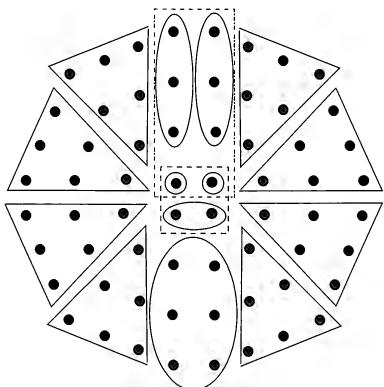
\includegraphics[width=0.62\textwidth]{figs/ch7s5-f64.jpg}
\caption{$\mathbb{F}_{64}$ 中 $x^{64}-x$ 的根按不可约因子聚类的示意 (两个虚线矩形分别框出其中唯一的 $\mathbb{F}_4$ 与 $\mathbb{F}_8$ 拷贝, 它们交于唯一的 $\mathbb{F}_2$ 拷贝).}
\end{figure}

两个虚线矩形框定包含在 $\mathbb{F}_{64}$ 中的 (唯一的) $\mathbb{F}_4$ 与 $\mathbb{F}_8$ 的拷贝; 它们交于 (唯一的) $\mathbb{F}_2$ 的拷贝.

再次, $\mathbb{F}_{64}$ 可以通过用任意一个 $6$ 次不可约多项式生成的理想来商 $\mathbb{F}_2[x]$ 而实现; 这给出了该域的 $9$ 个``不同''的实现.

上面为 $\mathbb{F}_{64}$ 所绘的图几乎毫无意义, 但它可以帮助我们聚焦我们将要提取的关于有限域的最后一点信息. 注意 $\mathbb{F}_{64}$ 的任意自同构的作用必是搅乱图中每个扇区所表示的元素, 而不混合不同扇区的元素, 也不交换扇区. 事实上, 一个扩张的每个自同构都把不可约多项式的根送到同一个多项式的根.

由于有限域的扩张都是单扩张, 我们先前的工作使我们能够精确得多. 把注意力限制在扩张 $\mathbb{F}_p\subseteq\mathbb{F}_{p^d}$ 上, 对素数 $p$, 我们知道这些可以通过一个极小多项式为 $d$ 次的元素实现为单扩张. 这个多项式必可分 ($\mathbb{F}_p$ 是完全的), 所以推论~\ref{cor:autk-count} 立即给出自同构群的大小:
\[
|\Aut_{\mathbb{F}_p}(\mathbb{F}_{p^d})|=d.
\]
但这个群是什么呢?

\begin{proposition}\label{prop:aut-cyclic-frobenius}
$\Aut_{\mathbb{F}_p}(\mathbb{F}_{p^d})$ 是循环群, 由 Frobenius 同构生成.
\end{proposition}

\begin{proof}
设 $\varphi$ 为 Frobenius 同态 $\mathbb{F}_{p^d}\to\mathbb{F}_{p^d}$: $\varphi(x)=x^p$. Frobenius 同态在有限域上是一个同构 (推论~\ref{cor:finite-fields-perfect}) 并且在 $\mathbb{F}_p$ 上限制为恒等 (习题~\ref{ex:frobenius-Fp-identity}), 所以 $\varphi\in\Aut_{\mathbb{F}_p}(\mathbb{F}_{p^d})$. 既然我们事先知道了这个群的大小, 所要证明的只是 $\varphi$ 的阶为 $d$.

设 $e=|\varphi|$. 则 $\varphi^e=\mathrm{id}$; 从而对所有 $x\in\mathbb{F}_{p^d}$ 有 $x^{p^e}=x$. 换言之, (非零) 多项式 $x^{p^e}-x$ 在 $\mathbb{F}_{p^d}$ 中有 $p^d$ 个根; 这推出 $p^d\leq p^e$ (引理~V.\ref{lem:roots-count}). 等价地, $d\leq e$, 得到
\[
|\Aut_{\mathbb{F}_p}(\mathbb{F}_{p^d})|\leq|\varphi|.
\]
但那样这两个数必相等, 因为一个元素的阶总整除群的阶 (习题~II.\ref{ex:lagrange-order}).
\end{proof}

关于有限域还有最后两点评论:
\begin{itemize}
\item[—] 对足够大的 $n$, 惊人地大 (但有限) 的域 $\mathbb{F}_{p^{n!}}$ 可作为代数闭包 $\overline{\mathbb{F}_p}$ 的一个近似: 事实上, 由推论~\ref{cor:factor-xqn}, 这个域包含 $\mathbb{F}_p[x]$ 中所有次数 $\leq n$ 的多项式的根.

这一观察可以转化为 $\overline{\mathbb{F}_p}$ 的一个显式构造: 由推论~\ref{cor:finite-field-extension} 存在扩张
\[
\mathbb{F}_p\subseteq\mathbb{F}_{p^2}\subseteq\mathbb{F}_{p^6}\subseteq\mathbb{F}_{p^{4!}}\subseteq\cdots
\]
并且这个域链的并集给出一个 $\overline{\mathbb{F}_p}$ 的拷贝\footnote{更形式化的构造需要正向极限的概念; 参见 §\hyperref[subsec:limits-colimits]{VIII.1.4}.}.
\item[—] 有限域构成一个范畴, 它 (由推论~\ref{cor:finite-field-extension}) 应强烈地让读者想起在习题~I.\ref{ex:divisibility-category} 中遇到的``玩具''范畴. 然而有一个重要区别: 在那个范畴中每个对象恰有一个自同构, 而我们已经验证有限域可以有许多自同构. 挑战: 读者在一个不同 (但相关) 的语境中遇到过非常相似的情形. 在哪里?
\end{itemize}

\subsection{分圆多项式与分圆域}\label{subsec:cyclotomic}

在前面几节中我们经常遇到 $\mathbb{C}$ 中的 $1$ 的根; 它们生成的扩张非常重要.

设 $n$ 为正整数. 我们将用 $\zeta_n$ 表示复数 $e^{2\pi i/n}$; 于是多项式 $x^n-1$ 在 $\mathbb{C}$ 中的 $n$ 个根就是 $\zeta_n$ 的 $n$ 个不同幂次; 它们构成 $\mathbb{C}$ 的乘法群的一个 $n$ 阶循环子群, 记为 $\mu_n$.\index[sym1]{41@$\mu_n$}\index[sym1]{69@$\zeta_n$}

形象地, $1$ 的根放置在以 $0$ 为中心的正 $n$ 边形的顶点上, 其中一个顶点在 $1$ 处.

\begin{figure}[ht]
\centering
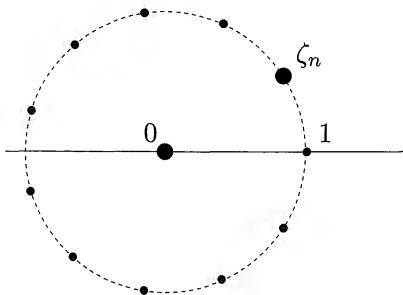
\includegraphics[width=0.4\textwidth]{figs/ch7s5-roots-of-unity.jpg}
\caption{单位根在正 $n$ 边形顶点上的分布.}
\end{figure}

$1$ 的一个 \emph{本原 $n$ 次根} 是 $\mu_n$ 的一个生成元. 于是 $\zeta_n$ 是本原的; 由我们对循环群的工作, 我们知道 (推论~II.\ref{cor:generates}) $\zeta_n^m$ 是一个本原 $n$ 次根当且仅当 $m$ 与 $n$ 互素. 特别地, 有 $\phi(n)$ 个本原的 $1$ 的根, 其中 $\phi$ 是 Euler $\varphi$ 函数 (参见习题~II.\ref{ex:euler-phi-sum}). 从而
\[
\Phi_n(x):=\prod_{\substack{1\leq m\leq n\\ (m,n)=1}}(x-\zeta_n^m)
\]
是一个 $\phi(n)$ 次的多项式.

\begin{definition}\label{def:cyclotomic-poly}
多项式 $\Phi_n(x)$ 称为第 $n$ 个 \emph{分圆多项式}.
\end{definition}

显然 $\Phi_n(x)$ 是一个 $\phi(n)$ 次的首一多项式. 也许不那么显然的是 $\Phi_n(x)$ 有有理 (事实上是整数) 系数, 并且在 $\mathbb{Q}$ 上不可约. 我们马上证明这些事实.

\begin{example}\label{ex:cyclotomic-prime}
若 $n=p$ 为素数, 则 $\mu_p\cong C_p$ 的每个非单位元素都是一个生成元: 除 $1$ 自身外每个 $p$ 次 $1$ 的根都是本原的. 因此
\[
\Phi_p(x)=\frac{x^p-1}{x-1}=x^{p-1}+\cdots+1
\]
就是在例~V.\ref{ex:cyclotomic-eisenstein} 中遇到的特例, 我们在那里证明了 $\Phi_p(x)$ 确实不可约.
\end{example}

如果 $n$ 不是素数呢?

\begin{lemma}\label{lem:cyclotomic-prod}
对所有正整数 $n$,
\[
x^n-1=\prod_{1\leq d\mid n}\Phi_d(x).
\]
\end{lemma}

\begin{proof}
若 $n=de$, 则每个 $d$ 次 $1$ 的根 $\zeta$ 都是 $n$ 次 $1$ 的根, 因为 $\zeta^n=\zeta^{de}=(\zeta^d)^e=1$. 特别地, 每个本原 $d$ 次 $1$ 的根 $\zeta$ 都是 $n$ 次 $1$ 的根.

另一方面, 每个 $\zeta\in\mu_n$ 生成一个子群 $H\subseteq\mu_n$, 且 $H=\mu_d$, 其中 $d$ 等于 $\zeta$ 的阶, 是 $n$ 的一个因子 (命题~II.\ref{prop:subgroups-zn}). 因此每个 $\zeta\in\mu_n$ 对某个 $d\mid n$ 是本原 $d$ 次 $1$ 的根.

由此 $n$ 次 $1$ 的根的集合等于所有 $d\mid n$ 的本原 $d$ 次 $1$ 的根的集合之并. 该陈述立得:
\[
x^n-1=\prod_{\zeta\in\mu_n}(x-\zeta)=\prod_{1\leq d\mid n}\Bigl(\prod_{\zeta\text{ 本原 }d\text{ 次根}}(x-\zeta)\Bigr)=\prod_{1\leq d\mid n}\Phi_d(x),
\]
如所断言.
\end{proof}

这一论证把我们带回到简单的群论考虑. 读者可以验证引理~\ref{lem:cyclotomic-prod} 通过比较所述恒等式两边的其次数立即推出习题~II.\ref{ex:euler-phi-sum} 的结果.

引理~\ref{lem:cyclotomic-prod} 给出了分圆多项式的一个归纳计算; 事实 $\Phi_n(x)\in\mathbb{Z}[x]$ 即由此事实推出. 显式地,

\begin{corollary}\label{cor:cyclotomic-int}
分圆多项式 $\Phi_n(x)$ 有整数系数.
\end{corollary}

\begin{proof}
对 $n$ 用归纳法. 注意 $\Phi_1(x)=x-1$, 并假设我们已经证明了所有 $m<n$ 的 $\Phi_m(x)$ 都有整数系数. 特别地,
\[
f(x):=\prod_{\substack{1\leq d\mid n\\ d<n}}\Phi_d(x)
\]
是一个有整数系数的首一多项式. 由于 $f(x)$ 首一, 我们可以在 $\mathbb{Z}[x]$ 中用它去除 $x^n-1$ 带余: $\exists\,q(x),r(x)\in\mathbb{Z}[x]$ 使得
\[
x^n-1=f(x)q(x)+r(x),
\]
其中 $r(x)=0$ 或 $\deg r(x)<\deg f(x)$. 另一方面, 由引理~\ref{lem:cyclotomic-prod},
\[
x^n-1=f(x)\Phi_n(x)
\]
在 $\mathbb{C}[x]$ 中. 因此在 $\mathbb{C}[x]$ 中
\[
f(x)\bigl(\Phi_n(x)-q(x)\bigr)=r(x).
\]
但这迫使 $r(x)=0$ (否则我们会有 $\deg r(x)\geq\deg f(x)$). 因此 $\Phi_n(x)=q(x)\in\mathbb{Z}[x]$.
\end{proof}

\begin{example}\label{ex:cyclotomic-examples}
读者可以花些高质量的时间显式计算几个非素数 $n$ 的分圆多项式 $\Phi_n(x)$, 用归纳法并利用我们已经知道素数的显式 $\Phi_p(x)$.

例如, $x^4-1=\Phi_1(x)\Phi_2(x)\Phi_4(x)$; 因此
\[
\Phi_4(x)=\frac{x^4-1}{x^2-1}=x^2+1.
\]
由于 $x^6-1=\Phi_1(x)\Phi_2(x)\Phi_3(x)\Phi_6(x)$,
\[
\Phi_6(x)=\frac{x^6-1}{(x^2-1)(x^2+x+1)}=x^2-x+1.
\]
由于 $x^{12}-1=\Phi_1(x)\Phi_2(x)\Phi_3(x)\Phi_4(x)\Phi_6(x)\Phi_{12}(x)$,
\[
\Phi_{12}(x)=\frac{x^{12}-1}{(x^6-1)(x^2+1)}=x^4-x^2+1,
\]
如此等等, 不一而足.

乐观的读者现在可能开始猜测 $\Phi_n(x)$ 的系数总是 $0$ 或 $\pm 1$ (如果我们不知道真相, 我们也会这样猜). 显然第一个反例出现在 $n=105$ (习题~\ref{ex:cyclotomic-1-15}); 并且已知当 $n\gg 0$ 时系数可以任意大.
\end{example}

$\Phi_n(x)$ 的不可约性稍微棘手一些, 特别是因为可分性溜进了标准论证 (这正是我们不得不等到现在才陈述它的原因).

\begin{proposition}\label{prop:cyclotomic-irred}
对所有正整数 $n$, $\Phi_n(x)\in\mathbb{Z}[x]$ 在 $\mathbb{Q}$ 上不可约.

(由于 $\Phi_n(x)$ 首一, 在 $\mathbb{Q}[x]$ 中的不可约性等价于在 $\mathbb{Z}[x]$ 中的不可约性; 参见推论~V.\ref{cor:irreducible-poly-equiv}.)
\end{proposition}

\begin{proof}
反证法, 假设 $\Phi_n(x)$ 可约. 则它的根 $\zeta_n^m$, 其中 $(m,n)=1$, 分布到各个因子中; 我们可以选取一个不可约首一因子 $f(x)$ 的一个根 $\zeta_n^m$, 使得另一个根 $\zeta_n^{mp}$ (对某个不整除 $n$ 的素数 $p$) 不是 $f(x)$ 的根. 写
\[
\Phi_n(x)=f(x)g(x);
\]
由于 $\Phi_n(x)\in\mathbb{Z}[x]$ 且 $\Phi_n(x)$, $f(x)$ 首一, 则 $f(x)$ 与 $g(x)$ 有整数系数 (参见习题~V.\ref{ex:poly-split-rx}). 由我们的选择, $f(x)$ 是 $\zeta_n^m$ 在 $\mathbb{Q}$ 上的极小多项式, 且 $g(\zeta_n^{mp})=0$.

由此 $\zeta_n^m$ 是 $g(x^p)$ 的一个根, 从而 $f(x)\mid g(x^p)$. 因此我们可以写
\[
g(x^p)=f(x)h(x)
\]
其中 $h(x)\in\mathbb{Z}[x]$. 把最后一个等式模 $p$ 读出来, 我们得到 (再次利用习题~\ref{ex:frobenius-Fp-identity}, 并用下划线表示陪集)
\[
\underline{g}(x)^p=\underline{f}(x)\underline{h}(x)\quad\text{在 }\mathbb{F}_p[x]\text{ 中};
\]
特别地, $\underline{f}(x)$ 与 $\underline{g}(x)$ 在 $\mathbb{F}_p[x]$ 中必有一个非平凡公因子 $\underline{\ell}(x)$. 但那样
\[
\underline{\ell}(x)^2\mid\underline{f}(x)\underline{g}(x):
\]
$\Phi_n(x)$ 模 $p$ 的归约必有一个重因子.

这推出 $x^n-1\in\mathbb{F}_p[x]$ 有一个重因子; 即它不可分. 然而它的导数 $nx^{n-1}\in\mathbb{F}_p[x]$ 非零 (因为由假设 $p$ 不整除 $n$), 而引理~\ref{lem:separable-gcd} 推出 $x^n-1$ 在 $\mathbb{F}_p[x]$ 中可分.

这一矛盾表明我们假设 $\Phi_n(x)$ 可约是荒谬的, 证明了该陈述. \qed
\end{proof}

\begin{definition}\label{def:cyclotomic-field}
多项式 $x^n-1$ 在 $\mathbb{Q}$ 上的分裂域 $\mathbb{Q}(\zeta_n)$ 是第 $n$ 个 \emph{分圆域}.
\end{definition}

由命题~\ref{prop:cyclotomic-irred}, $\mathbb{Q}(\zeta_n)$ 是 $\mathbb{Q}$ 的一个 $\phi(n)$ 次扩张; $\Phi_n(x)$ 是 $\zeta_n$ 的极小多项式.

像往常一样, 我们现在关注这个扩张的自同构群, 并且像在先前的例子中一样情形非常清晰.

\begin{proposition}\label{prop:aut-cyclotomic}
$\Aut_{\mathbb{Q}}(\mathbb{Q}(\zeta_n))$ 同构于 $\mathbb{Z}/n\mathbb{Z}$ 中的单位群.
\end{proposition}

\begin{proof}
我们知道 $\Aut_{\mathbb{Q}}(\mathbb{Q}(\zeta_n))$ 的基数为 $\phi(n)$ (推论~\ref{cor:autk-count}; 根互异因为 $\Phi_n(x)$ 可分), 所以我们只要给出一个单同态
\[
j:(\mathbb{Z}/n\mathbb{Z})^*\to\Aut_{\mathbb{Q}}(\mathbb{Q}(\zeta_n)).
\]
对 $[m]_n\in(\mathbb{Z}/n\mathbb{Z})^*$, 即对一个与 $n$ 互素的整数 $m$, 令 $j([m]_n)$ 为唯一的把 $\zeta_n$ 送到 $\zeta_n^m$ 的 $\mathbb{Q}(\zeta_n)\to\mathbb{Q}(\zeta_n)$ 的自同构 (参见命题~\ref{prop:simple-ext-iso-lift});
这显然与代表元 $m$ 的选择无关. 则 $j$ 显然单, 且
\[
j([m_1]_n)\circ j([m_2]_n)(\zeta_n)=j([m_1]_n)(\zeta_n^{m_2})=\zeta_n^{m_2m_1}
\]
与 $j([m_1m_2]_n)$ 的作用一致, 表明 $j$ 是一个同态, 完成证明. \qed
\end{proof}

\begin{example}\label{ex:splitting-x8-1-aut}
读者应当重新考虑例~\ref{ex:x8-1-splitting}: 由我们刚刚证明的, $x^8-1$ 的分裂域的自同构群同构于 $\mathbb{Z}/8\mathbb{Z}$ 中的单位群; 这个群立刻可见同构于 $(\mathbb{Z}/2\mathbb{Z})\times(\mathbb{Z}/2\mathbb{Z})$, 确认了例~\ref{ex:x8-1-splitting} 中作出的断言.
\end{example}

正 $n$ 边形用直尺与圆规的可构造性当然等价于复数 $\zeta_n$ 的可构造性. 既然我们现在知道 $[\mathbb{Q}(\zeta_n):\mathbb{Q}]=\phi(n)$, 推论~\ref{cor:constructible-degree} 告诉我们正 $n$ 边形能用直尺与圆规构造仅当 $\phi(n)$ 是 $2$ 的幂. 这个条件可以追得更远 (习题~\ref{ex:regular-n-gon-constructible}). 无论如何, 在我们吸收了一点 Galois 理论之后, 我们将再次回到这个主题.

\subsection{可分性与单扩张}\label{subsec:separability-simple}

我们迄今遇到的所有域扩张的例子都是单扩张, 尽管有时这起初并不完全明显 (参见例~\ref{ex:sqrt2-sqrt3}). 这有一个很好的理由: 我们看到的大多数例子都是可分扩张, 而我们现在可以证明一个有限可分扩张必是单的.

这里是一个单扩张的漂亮判据 (它不涉及任何可分性条件):

\begin{proposition}\label{prop:simple-inter-finite}
一个代数扩张 $k\subseteq F$ 是单的当且仅当不同的中间域 $k\subseteq E\subseteq F$ 的数目有限.
\end{proposition}

\begin{proof}
假设 $F=k(\alpha)$ 是单且代数的, 并设 $q_k(x)$ 为 $\alpha$ 在 $k$ 上的极小多项式. 把 $F$ 嵌入 $k$ 的一个代数闭包 $\overline{k}$ 中. 若 $E$ 是一个中间域, 则 $F=E(\alpha)$ 也是一个单的、代数的扩张; 记 $q_E(x)$ 为 $\alpha$ 在 $E$ 上的极小多项式. 由于对所有 $E$ 有 $q_k(x)\in E[x]$ 且 $q_k(\alpha)=0$, 我们知道每个 $q_E(x)$ 是 $q_k(x)$ 的一个因子.

我们断言 $E$ 其实由 $q_E(x)$ 决定. 由于 $q_k(x)$ 在 $\overline{k}$ 中只有有限多个因子, 这就证明了只有有限多个中间域, 即陈述的``仅当''部分.

为验证我们的断言, 我们将证明 $E$ 由 $q_E(x)$ 的系数 (在 $k$ 上) 生成. 为看清这一点, 令 $E'$ 为 $E$ 中由 $k$ 与 $q_E(x)$ 的系数生成的子域. 则 $q_E(x)\in E'[x]$, 并且由于 $q_E(x)$ 在 $E$ 上不可约, 它在 $E'$ 上必不可约. 注意 $E'(\alpha)=F=E(\alpha)$. 我们有 $E'\subseteq E\subseteq F$; 因此
\[
\deg(q_E(x))=[F:E']=[F:E][E:E']=\deg(q_E(x))[E:E'],
\]
由此 $[E:E']=1$; 即 $E=E'$, 如所需. 这就完成了陈述的``仅当''部分的证明.

为证明``当''部分, 假设只有有限多个中间域 $k\subseteq E\subseteq F$. 扩张 $k\subseteq F$ 必是有限生成的 (否则我们可以构造一个无限子扩张链 $k\subseteq k(\alpha_1)\subseteq k(\alpha_1,\alpha_2)\subseteq\cdots\subseteq F$, 从而会有无限多个中间域), 因此由于它是代数的而是有限的. 若 $k$ 是有限域, 则 $F$ 也是, 并且该扩张由推论~\ref{cor:finite-field-extension} 自动是单的; 因此我们可以假设 $k$ 是无限的, 并且我们要证明每个有限生成的代数扩张 $F=k(\alpha_1,\ldots,\alpha_r)$ 是单的.

用归纳法, 我们不妨设 $F=k(\alpha,\beta)$. 对每个 $c\in k$, 我们有中间域
\[
k(c\alpha+\beta)\subseteq k(\alpha,\beta).
\]
但只有有限多个中间域, 而 $k$ 是无限的, 所以对某些 $c\neq c'\in k$ 必有
\[
k(c'\alpha+\beta)=k(c\alpha+\beta).
\]
由此
\[
\alpha=\frac{(c'\alpha+\beta)-(c\alpha+\beta)}{c'-c}\in k(c\alpha+\beta)\quad\text{且}\quad\beta=(c\alpha+\beta)-c\alpha\in k(c\alpha+\beta)
\]
因此 $k(\alpha,\beta)\subseteq k(c\alpha+\beta)$. 另一包含平凡成立, 所以 $k(\alpha,\beta)=k(c\alpha+\beta)$ 是单的.
\end{proof}

这里是与可分性的联系:

\begin{proposition}\label{prop:finite-sep-simple}
每个有限可分扩张都是单的.
\end{proposition}

\begin{proof}
像命题~\ref{prop:simple-inter-finite} 的证明中那样用归纳法, 我们不妨设 $F=k(\alpha,\beta)$, 其中 $\alpha$ 与 $\beta$ 在 $k$ 上可分 (从而特别地是代数的), 并且我们可以假设 $k$ 是无限域.

考虑嵌入 $\iota:F\hookrightarrow\overline{k}$ 的集合 $I$, 即 $F$ 到 $k$ 的代数闭包中、扩张 $k$ 的恒等的嵌入. 若 $\iota\neq\iota'\in I$ 且 $x$ 是一个不定元, 则多项式
\[
\iota(\alpha)x+\iota(\beta),\qquad\iota'(\alpha)x+\iota'(\beta)
\]
是不同的: 否则 $\iota'(\alpha)=\iota(\alpha)$ 且 $\iota'(\beta)=\iota(\beta)$, 从而 $\iota,\iota'$ 会在整个 $k(\alpha,\beta)$ 上以相同方式作用, 迫使 $\iota=\iota'$.

\index{duoxiangshi@多项式(polynomial)!shouyi@首一(monic)}因此多项式
\[
f(x)=\prod_{\iota\neq\iota'}\bigl((\iota(\alpha)x+\iota(\beta))-(\iota'(\alpha)x+\iota'(\beta))\bigr)\in\overline{k}[x]
\]
不恒为 $0$. 由于 $k$ 无限, 由此 $\exists\,c\in k$ 使得 $f(c)\neq 0$; 即不同的 $\iota\in I$ 把
\[
\gamma=c\alpha+\beta
\]
送到不同的元素
\[
\iota(\gamma)=\iota(\alpha)c+\iota(\beta)
\]
(每个 $\iota$ 扩张 $\mathrm{id}_k$, 所以 $\iota(c)=c$). 由于 $I$ 的基数为 $[F:k]_s$ (定义~\ref{def:separable-degree}) 且每个 $\iota(\gamma)$ 是 $\gamma$ 在 $k$ 上的极小多项式的一个根, 我们有
\[
[F:k]_s\leq[k(\gamma):k]\leq[F:k].
\]
由假设该扩张可分, 所以由命题~\ref{prop:finite-sep-degree} 知 $[F:k]_s=[F:k]$, 推出 $[k(\gamma):k]=[F:k]$ 并最后
\[
F=k(\gamma),
\]
完成证明.
\end{proof}

命题~\ref{prop:finite-sep-simple} 很好地说明了为什么可分性是一个技术上令人满意的条件. 为了更进一步强调这一点, 注意我们现在可以把推论~\ref{cor:autk-count} 中找到的方便的不等式推广到所有有限可分扩张:

\begin{corollary}\label{cor:aut-ineq}
设 $k\subseteq F$ 为一个有限、可分扩张. 则
\[
|\Aut_k(F)|\leq[F:k],
\]
等号成立当且仅当 $k\subseteq F$ 是正规扩张.
\end{corollary}

\begin{proof}
由于 $k\subseteq F$ 有限且可分, 命题~\ref{prop:finite-sep-simple} 推出它是单的: 对某个 $\alpha\in F$ 有 $F=k(\alpha)$. 该不等式由推论~\ref{cor:autk-count} 立得, 且等号成立当且仅当 $\alpha$ 的极小多项式 $f(x)$ 在 $F$ 中分解为互异的一次因子. 在此情形下 $F$ 是 $f(x)$ 的分裂域, 所以由定理~\ref{thm:finite-normal-splitting} 它在 $k$ 上正规. 反过来, 若 $F$ 在 $k$ 上正规, 则 $f(x)$ 在 $F$ 中完全分裂并且由于 $\alpha$ 在 $k$ 上可分而有互异的根; 因此 $|\Aut_k(F)|=[F:k]$, 再次由推论~\ref{cor:autk-count}. \qed
\end{proof}

\begin{example}\label{ex:non-simple-insep}
由命题~\ref{prop:finite-sep-simple}, 如果我们想构造一个非单的有限扩张, 我们必须使用不可分元素; 为给出一个例子, 我们把例~\ref{ex:xp-t-insep} 稍微加工一下. 考虑两个变量上的有理函数域 $F=\mathbb{F}_p(u,v)$ 与子域 $k=\mathbb{F}_p(s,t)$, 其中 $s=u^p$ 且 $t=v^p$. 则 $k\subseteq F$ 是一个代数扩张; $u$ 在 $k$ 上的极小多项式是 $x^p-s$; $v$ 在 $k(u)$ 上的极小多项式是 $y^p-t$; 由此
\[
[F:k]=p^2.
\]
当 $c$ 取遍 $k$ 时, 我们得到中间域
\[
k\subseteq k(cu+v)\subseteq F.
\]
若任意两个选择 $c$, $c'$ 导致相同的中间域, 则我们会像命题~\ref{prop:simple-inter-finite} 的证明中那样推出 $k(u,v)=k(cu+v)$. 特别地, 我们会有
\[
[k(cu+v):k]=p^2.
\]
但事实并非如此, 因为 $(cu+v)^p=c^ps+t\in k(s,t)=k$; 从而 $cu+v$ 在 $k$ 上的极小多项式的次数至多为 $p$. 由于 $k=\mathbb{F}_p(s,t)$ 无限, 有无限多个中间域, 并由此 (由命题~\ref{prop:simple-inter-finite}) 推出 $F$ 不是 $k$ 的一个单扩张.
\end{example}

\subsection*{习题}
\phantomsection
\addcontentsline{toc}{subsection}{习题}

\begin{prob}\label{ex:finite-field-additive}
设 $p>0$ 为素数. 证明阶为 $p^d$ 的有限域的加法群同构于 $(\mathbb{Z}/p\mathbb{Z})^d$.
\end{prob}

\begin{prob}\label{ex:sum-of-two-squares}
证明有限域 $F$ 的每个元素都是 $F$ 中两个平方之和. (提示: 记住 $F$ 的乘法群是循环的.)
\end{prob}

\begin{prob}\label{ex:finite-field-iso-F8}
$\triangleright$ 找出一个显式同构
\[
\frac{\mathbb{F}_2[x]}{(x^3+x^2+1)}\xrightarrow{\sim}\frac{\mathbb{F}_2[x]}{(x^3+x+1)}.
\]
[§\ref{subsec:finite-fields}]
\end{prob}

\begin{prob}\label{ex:irred-deg4-F2}
$\triangleright$ 找出 $\mathbb{F}_2$ 上所有 $4$ 次不可约多项式, 并数出 $5$ 次的个数. [§\ref{subsec:finite-fields}]
\end{prob}

\begin{prob}\label{ex:irred-deg12-F9}
找出 $\mathbb{F}_9$ 上 $12$ 次不可约多项式的数目.
\end{prob}

\begin{prob}\label{ex:F16-frobenius-action}
用 $\mathbb{F}_{16}$ 作为 $\mathbb{F}_2[x]$ 的商的任一实现, 显式写出循环群 $C_4$ 在 $\mathbb{F}_{16}$ 上的作用 (即作为 $\mathbb{F}_2$-向量空间的线性变换).
\end{prob}

\begin{prob}\label{ex:frobenius-rational-canonical}
设 $p$ 为素数. 把 Frobenius 自同构 $\varphi:\mathbb{F}_{p^d}\to\mathbb{F}_{p^d}$ 视为 $\mathbb{F}_{p^d}$ 的 $\mathbb{F}_p$-向量空间上的线性变换. 找出 $\varphi$ 的有理标准形. (改造命题~\ref{prop:aut-cyclic-frobenius} 的证明以说明 $\varphi$ 的极小多项式是 $x^d-1$.)
\end{prob}

\begin{prob}\label{ex:factor-Phi-p-Fp}
对素数 $p$, 找出 $\Phi_p(x)$ 在 $\mathbb{F}_p$ 上的分解.
\end{prob}

\begin{prob}\label{ex:cyclotomic-1-15}
$\triangleright$ 找出所有 $1\leq n\leq 15$ 的分圆多项式 $\Phi_n(x)$. 计算 $\Phi_{105}(x)$. [§\ref{subsec:cyclotomic}]
\end{prob}

\begin{prob}\label{ex:cyclotomic-2m}
找出所有 $m\geq 0$ 的 $\Phi_{2^m}(x)$.
\end{prob}

\begin{prob}\label{ex:Phi-2n-Phi-n}
证明若 $n>1$ 为奇数, 则 $\Phi_{2n}(x)=\Phi_n(-x)$. (提示: 把本原 $14$ 次 $1$ 的根与本原 $7$ 次 $1$ 的根并列画出; 然后回到习题~II.\ref{ex:euler-phi-odd} 以证明你所观察到的现象.)
\end{prob}

\begin{prob}\label{ex:Phi-n-divides}
$\neg$ 设 $a,n$ 为正整数, 且 $a>1$. 证明若 $\Phi_n(a)$ 整除 $a-1$, 则 $n=1$. (记住 $\Phi_n(a)$ 是复数 $a-\zeta$ 的乘积, 其中 $\zeta$ 是本原 $n$ 次 $1$ 的根. 这告诉你关于 $\Phi_n(a)$ 的大小的什么信息?) [命题~\ref{prop:cyclotomic-irred}]
\end{prob}

\begin{prob}\label{ex:Phi-n-quotient}
$\neg$ 设 $a,d,n$ 为正整数, 且 $d<n$, $a>1$. 假设 $a^d-1$ 整除 $a^n-1$. 证明 $\Phi_n(a)$ 整除商 $(a^n-1)/(a^d-1)$. (提示: 习题~V.\ref{ex:ca-1-divides}.) [命题~\ref{prop:cyclotomic-irred}]
\end{prob}

\index{Witt@Witt!Ernst@Ernst}\begin{prob}\label{ex:wedderburn-witt}
$\triangleright$ 设 $R$ 为一个有限除环.
\begin{itemize}
\item 证明 $R$ 的中心 (习题~III.\ref{ex:center}) 同构于 $\mathbb{F}_q$, 其中 $q$ 为素数幂. 证明 $|R|=q^n$ 对某个 $n$.
\item 对每个 $r\in R$, 证明 $(R^*,\cdot)$ 的乘法群中 $r$ 的中心化子的阶为 $q^d-1$ 对某个 $d\leq n$.
\item 证明存在整数 $d_1,\ldots,d_r<n$ 使得
\begin{equation}
q^n-1=q-1+\sum_{i=1}^r\frac{q^n-1}{q^{d_i}-1}.
\tag{*}\end{equation}
(提示: 类方程.)
\item 推出 $\Phi_n(q)$ 整除 $q-1$, 从而 $n=1$. (利用习题~\ref{ex:Phi-n-divides} 与 \ref{ex:Phi-n-quotient}.)
\item 推出 $R$ 等于其中心, 表明 $R$ 是交换的.
\end{itemize}
\index{Wedderburn@Wedderburn!Joseph@Joseph!xiaodingli@小定理(little theorem)!xiemi@楔幂(wedge power)}于是每个有限除环都是一个域: 这就是 Wedderburn 的小定理. 这里给出的论证属于 Ernst Witt. [§III.\ref{subsec:ring-examples}]
\end{prob}

\begin{prob}\label{ex:Phi-n-mod-p}
$\triangleright$ 设 $a,p,n$ 为整数, 其中 $p,n$ 为正且 $p$ 为素数, $p\nmid n$.
\begin{itemize}
\item 证明 $x^n-1$ 模 $p$ 无重根.
\item 证明若 $p$ 整除 $\Phi_n(a)$, 则 $a^n\equiv 1\pmod p$. (特别地, $p\nmid a$, 故 $[a]_p\in(\mathbb{Z}/p\mathbb{Z})^*$.)
\item 证明若 $p$ 整除 $\Phi_n(a)$, 则对一切 $d<n$ 有 $a^d\not\equiv 1\pmod p$.
\item 推出 $p\mid\Phi_n(a)$ 当且仅当 $[a]_p$ 在 $(\mathbb{Z}/p\mathbb{Z})^*$ 中的阶为 $n$.
\item 计算 $\Phi_{15}(9)$, 并证明它被 $31$ 整除. 然后回看习题~II.\ref{ex:order-9-31} 的第一部分.
\end{itemize}
[§II.\ref{subsec:iso-groups}, 习题~\ref{ex:primitive-prime-divisor}, 习题~\ref{ex:p-congruence-1-mod-n}]
\end{prob}

\begin{prob}\label{ex:primitive-prime-divisor}
\index{Birkhoff–Vandiver dingli@Birkhoff–Vandiver 定理(Birkhoff-Vandiver theorem)}若 $q$ 是一个整除 $a^n-1$ 且对任意 $d<n$ 不整除 $a^d-1$ 的素数, 则称 $q$ 为 $a^n-1$ 的一个 \emph{本原素因子}. 由习题~\ref{ex:Phi-n-mod-p}, 若 $q\nmid n$ 且 $q\mid\Phi_n(a)$, 则 $q$ 是 $a^n-1$ 的一个本原素因子. Birkhoff--Vandiver 定理断言 $a^n-1$ 对所有但极少数例外都有本原素因子: $n=1$, $a=2$; $n=2$, $a+1$ 是 $2$ 的幂; 以及 $n=6$, $a=2$.

\index{Lichiardopol@Lichiardopol!Nicolas@Nicolas}假设这一陈述, 我们可以给出 Wedderburn 定理的另一个证明 (由 Nicolas Lichiardopol 于 $2003$ 年发表). 设 $R$ 为一个有限除环.
\begin{itemize}
\item 证明存在素数 $p$ 使得 $|R|=p^n$ 对某个整数 $n$.
\item 若 $n=1$, 则 $R\cong\mathbb{F}_p$. 若 $n=2$ 或 $p=2$ 且 $n=6$, 则 $R$ 是交换的: 读者已在习题~III.\ref{ex:division-p2} 与 IV.\ref{ex:wedderburn-64} 中证明了这一点.
\item 因此, 由 Birkhoff--Vandiver 我们不妨假设 $p^n-1$ 有一个本原素因子 $p'$.
\item 证明在 $R$ 的乘法群 $(R^*,\cdot)$ 中存在一个阶为 $p'$ 的元素 $a$.
\item 证明 $R$ 是包含 $a$ 的 $R$ 的唯一子除环.
\item 证明 $a$ 在 $R$ 中的中心化子 (习题~III.\ref{ex:centralizer}) 就是 $R$ 自身; 推出 $a$ 在 $R$ 的中心中 (习题~III.\ref{ex:center}).
\item 证明 $R$ 的中心就是 $R$: 这表明 $R$ 是交换的.
\end{itemize}
于是 $R$ 是一个有限域.

注意 Birkhoff--Vandiver 定理给出了另一个快速方式来完成 Witt 的证明: $q^n-1$ 的一个本原素因子会由 $(*)$ 整除 $q-1$, 表明 $n=1$.
\end{prob}

\begin{prob}\label{ex:p-congruence-1-mod-n}
$\neg$ 设 $a,p,n$ 为整数, 其中 $p,n$ 为正且 $p$ 为素数, $p\nmid n$. 假设 $p$ 整除 $\Phi_n(a)$. 证明 $p\equiv 1\bmod n$. (利用习题~\ref{ex:Phi-n-mod-p}.) [习题~\ref{ex:inf-many-primes-1-mod-n}]
\end{prob}

\begin{prob}\label{ex:inf-many-primes-1-mod-n}
$\triangleright$ 设 $n>0$ 为任意整数. 证明存在无穷多个素数整数 $\equiv 1\bmod n$. (利用习题~\ref{ex:p-congruence-1-mod-n} 与习题~V.\ref{ex:euclid-variation-primes}.)

\index{Dirichlet@Dirichlet!Peter Gustav Lejeune@Peter Gustav Lejeune}这一练习的结果就是 Dirichlet 关于算术级数中的素数的定理的一个特例; 参见 §\ref{subsec:abelian-galois-q}. [\S\ref{subsec:abelian-galois-q}]
\end{prob}

\begin{prob}\label{ex:regular-n-gon-constructible}
$\triangleright$ 证明正 $n$ 边形能用直尺与圆规构造仅当 $n=2^m p_1\cdots p_r$, 其中 $m\geq 0$ 且因子 $p_i$ 是互异的 Fermat 素数. (提示: 利用习题~V.\ref{ex:zn-crt-phi} 与推论~\ref{cor:constructible-degree}.) [§\ref{subsec:cyclotomic}, §\ref{subsec:constructible-ngons}]
\end{prob}

\begin{prob}\label{ex:matrix-contains-extension-finite}
回忆由习题~\ref{ex:matrix-contains-extension}, $k$ 上次数 $\leq n$ 的每个域扩张都是矩阵环 $\mathcal{M}_n(k)$ 的一个子 $k$-代数. 证明若 $k$ 有限或特征为 $0$, 则包含在 $\mathcal{M}_n(k)$ 中的每个 $k$ 的扩张都有次数 $\leq n$.
\end{prob}

\begin{prob}\label{ex:splitting-of-separable}
证明若 $k\subseteq F$ 是一个可分多项式的分裂域, 则它也是一个不可约可分多项式的分裂域.
\end{prob}

\begin{prob}\label{ex:separable-generation}
$\neg$ 设 $k$ 为无限域. 若 $F=k(\alpha_1,\ldots,\alpha_r)$, 其中每个 $\alpha_i$ 在 $k$ 上可分, 证明存在 $c_1,\ldots,c_r\in k$ 使得 $F=k(c_1\alpha_1+\cdots+c_r\alpha_r)$.
\end{prob}

\begin{prob}\label{ex:no-irred-no-sep-extension}
$\triangleright$ 设 $k$ 为一个域, 并设 $n>0$ 为整数. 假设在 $k[x]$ 中不存在 $n$ 次不可约多项式. 证明不存在 $k$ 的 $n$ 次可分扩张. [§\ref{subsec:ft-algebra}]
\end{prob}

\section{一点 Galois 理论}\label{sec:galois-theory}

Galois 理论是域论与群论之间优美的交互, 其动机最初来自确定多项式根之间``对称性''的问题. Galois 关心的是多项式的根之间必然成立的具体关系, 其中最平凡的例子莫过于: 若 $\alpha,\beta$ 是 $x^2+px+q$ 的根, 则 $\alpha+\beta=-p$ 且 $\alpha\beta=q$. 交换根 $\alpha,\beta$ 对量 $\alpha+\beta,\alpha\beta$ 毫无影响. 更一般地, 对高次多项式, 可能存在若干在根的某些置换下保持不变的量. 这些量以及相应的置换群可以看作由该多项式决定的不变量, 从而给出一个研究该多项式的精妙工具.

\subsection{Galois 对应与 Galois 扩张}\label{subsec:galois-correspondence}

在域论的语言中, 多项式 $f(x)$ 的根的子集决定了 $f(x)$ 分裂域的中间域, 而根的置换群给出这些中间域的自同构. 有见于此, 分裂域走到台前毫不意外; 我们能够用自同构群刻画此类域 (下述定理~\ref{thm:galois-equivalence}) 这一事实, 将是整个讨论的关键.

在涉入这些水域之前, 我们应当把扩张的自同构群与中间域之间的精确关系形式化.

\begin{definition}\label{def:fixed-field}
\index{budongyu@不动域(fixed field)}设 $k\subseteq F$ 为域扩张, 并设 $G\subseteq\Aut_k(F)$ 是此扩张的一个自同构群. $G$ 的\emph{不动域}是中间域\index[sym1]{04@$\Aut_k(F)$}
\[
F^G:=\{\alpha\in F\mid \forall g\in G,\; g\alpha=\alpha\}.
\]
$F^G$ 确实是包含 $k$ 的 $F$ 的子域, 这一点是显然的. 不动域的概念使我们可以建立一个对应
\[
\begin{tikzcd}[column sep=3em]
\{\text{中间域 }E:k\subseteq E\subseteq F\} \ar[r,shift left=.7ex] & \{\Aut_k(F)\text{ 的子群}\} \ar[l,shift left=.7ex]
\end{tikzcd},
\]
它把中间域 $E$ 映到 $\Aut_k(F)$ 的子群 $\Aut_E(F)$, 把子群 $G\subseteq\Aut_k(F)$ 映到不动域 $F^G$.
\end{definition}

\begin{definition}\label{def:galois-correspondence}
这被称为 \emph{Galois 对应}.
\end{definition}

\begin{lemma}\label{lem:galois-correspondence-inclusion}
Galois 对应是反包含的. 进一步, 对 $\Aut_k(F)$ 的所有子群 $G$ 与所有中间域 $k\subseteq E\subseteq F$:
\begin{itemize}
\item $E\subseteq F^{\Aut_E(F)}$;
\item $G\subseteq\Aut_{F^G}(F)$.
\end{itemize}
此外, 记 $E_1E_2$ 为包含中间域 $E_1,E_2$ 的 $F$ 的最小子域, 记 $\langle G_1,G_2\rangle$ 为包含子群 $G_1,G_2$ 的 $\Aut_k(F)$ 的最小子群. 则
\begin{itemize}
\item $\Aut_{E_1E_2}(F)=\Aut_{E_1}(F)\cap\Aut_{E_2}(F)$;
\item $F^{\langle G_1,G_2\rangle}=F^{G_1}\cap F^{G_2}$.
\end{itemize}
\end{lemma}

\begin{proof}
习题~\ref{ex:galois-ft-lemma}.
\end{proof}

当然, 读者应当开始猜想: 是否存在某些情形能保证引理~\ref{lem:galois-correspondence-inclusion} 中的包含关系成为等式, 从而使 Galois 对应成为双射. 这正是我们前进的方向. 第一个观察是这并非总成立:

\begin{example}\label{ex:cube-root-2-not-galois}
考虑扩张 $\mathbb{Q}\subseteq\mathbb{Q}(\sqrt[3]{2})$. 由于
\[
[\mathbb{Q}(\sqrt[3]{2}):\mathbb{Q}]=3
\]
是素数, 唯一的中间域是 $\mathbb{Q}$ 与 $\mathbb{Q}(\sqrt[3]{2})$ (由推论~\ref{cor:degree-divides}). 关于 $\Aut_{\mathbb{Q}}(\mathbb{Q}(\sqrt[3]{2}))$, 由于 $\sqrt[3]{2}\in\mathbb{R}$, 我们有一个扩张 $\mathbb{Q}(\sqrt[3]{2})\subseteq\mathbb{R}$; 又由于 $\sqrt[3]{2}$ 是 $\mathbb{R}$ 中 $2$ 的唯一立方根, 我们看到 $\sqrt[3]{2}$ 的极小多项式 $t^3-2$ 在 $\mathbb{Q}(\sqrt[3]{2})$ 中只有一个根. 由推论~\ref{cor:autk-count}, $\Aut_{\mathbb{Q}}(\mathbb{Q}(\sqrt[3]{2}))$ 由单个元素组成: 它是平凡的.

\index{dandianji@单点集(singleton)}于是, 在此例中 Galois 对应在两个元素组成的集合与单点集之间作用:
\[
\begin{tikzcd}[column sep=3em]
\{\mathbb{Q},\mathbb{Q}(\sqrt[3]{2})\} \ar[r,shift left=.7ex] & \{\Aut_{\mathbb{Q}}(\mathbb{Q}(\sqrt[3]{2}))\}=\{e\} \ar[l,shift left=.7ex]
\end{tikzcd}.
\]
特别地, 把每个中间域映到相应自同构群的函数一般不是单射.

这个例子表明引理~\ref{lem:galois-correspondence-inclusion} 中的包含 $E\subseteq F^{\Aut_E(F)}$ 可能是真包含: $\mathbb{Q}$ 真包含于 $\mathbb{Q}(\sqrt[3]{2})$, 而后者是自同构群 (唯一) 子群的不动域. 所幸, 另一个包含关系受到更多限制:
\end{example}

\begin{proposition}\label{prop:aut-fixed-field-degree}
设 $k\subseteq F$ 为有限扩张, 并设 $G$ 是 $\Aut_k(F)$ 的一个子群. 则 $|G|=[F:F^G]$, 且
\[
G=\Aut_{F^G}(F).
\]
特别地, 对有限扩张, Galois 对应 (从中间域到自同构群) 是满射.
\end{proposition}

证明这一事实引导我们仔细考察形如 $F^G\subseteq F$ 的有限扩张. 出人意料的是, 它们恰好满足我们迄今遇到的几乎所有性质:

\begin{lemma}\label{lem:fixed-field-ext-props}
设 $k\subseteq F$ 为有限扩张, 并设 $G$ 是 $\Aut_k(F)$ 的一个子群. 则 $F^G\subseteq F$ 是有限, 单, 正规, 可分的扩张.
\end{lemma}

\begin{remark}\label{rmk:galois-orbit-poly}
本引理的关键在于如下值得强调的观察.

若 $\alpha\in F$ 且 $g\in G$, 注意 $g\alpha$ 必是 $\alpha$ 在 $k$ 上的极小多项式的根; 根只有有限多个, 所以 $G$ 在 $\alpha$ 上的轨道由有限多个元素 $\alpha=\alpha_{1},\ldots,\alpha_{n}$ 组成. 群 $G$ 通过置换这些元素来作用此轨道; 因此, $G$ 的每个元素都保持多项式
\[
q_\alpha(t)=(t-\alpha_{1})\cdots(t-\alpha_{n})
\]
不变. 换言之, 此多项式的系数必属于不动域 $F^G$. 进一步, $q_\alpha(t)$ 是可分的, 因为它有互异的根. 最后注意 $\deg q_\alpha(t)\leq |G|$.

有见于此, 我们准备证明该引理.
\end{remark}

\begin{proof}[引理~\ref{lem:fixed-field-ext-props} 的证明]
扩张 $F^G\subseteq F$ 是有限的, 因为 $k\subseteq F$ 是有限的.

设 $\alpha\in F$; 由引理陈述后的注记, $\alpha$ 是系数在 $F^G$ 中的一个可分多项式 $q_\alpha(t)$ 的根. 由此推出 $\alpha$ 在 $F^G$ 上是可分的; 因此根据定义~\ref{def:separable-poly}, 该扩张是可分的.

由于 $F^G\subseteq F$ 有限且可分, 由命题~\ref{prop:finite-sep-simple} 它是单的, 令 $\alpha$ 为生成元. 多项式 $q_\alpha(t)$ 在 $F$ 中分裂, 且 $F$ 由 $q_\alpha(t)$ 的根在 $F^G$ 上生成 (实际上, $\alpha_{1}=\alpha$ 就足以在 $F^G$ 上生成 $F$); 因此根据定义~\ref{def:splitting-field}, $F$ 是 $q_\alpha(t)$ 在 $F^G$ 上的分裂域. 于是由定理~\ref{thm:finite-normal-splitting}, $F^G\subseteq F$ 是正规的, 证毕.
\end{proof}

命题~\ref{prop:aut-fixed-field-degree} 是引理~\ref{lem:fixed-field-ext-props} 的推论:

\begin{proof}[命题~\ref{prop:aut-fixed-field-degree} 的证明]
由引理~\ref{lem:galois-correspondence-inclusion}, $G$ 是 $\Aut_{F^G}(F)$ 的子群, 特别地
\[
|G|\leq|\Aut_{F^G}(F)|.
\]
为验证 $G=\Aut_{F^G}(F)$, 只需证明反向不等式. 由引理~\ref{lem:fixed-field-ext-props}, $F=F^G(\alpha)$ 对某个 $\alpha\in F$; 因此 $|\Aut_{F^G}(F)|$ 等于 $\alpha$ 在 $F^G$ 上的极小多项式在 $F$ 中互异根的个数 (由推论~\ref{cor:autk-count}). 采用注记~\ref{rmk:galois-orbit-poly} 中的记号, $\alpha$ 是 $q_\alpha(x)\in F^G[x]$ 的根; 因此 $\alpha$ 的极小多项式是 $q_\alpha(x)$ 的因子. 由于构造上 $q_\alpha(x)$ 的根的个数为 $\leq |G|$, 我们得到
\[
|\Aut_{F^G}(F)|\leq |G|,
\]
如所需.

为验证 $[F:F^G]=|G|$, 只需注意由推论~\ref{cor:aut-ineq}, $[F:F^G]=|\Aut_{F^G}(F)|$, 因为根据引理~\ref{lem:fixed-field-ext-props} $F^G\subseteq F$ 是正规且可分的.
\end{proof}

\begin{remark}\label{rmk:infinite-galois}
命题~\ref{prop:aut-fixed-field-degree} 中扩张为有限的假设是必要的: 在无限情形 Galois 对应未必是满射. 但并未全失: 可以给自同构群赋予适当的拓扑, 并把 Galois 对应限制到自同构群的闭子群上, 从而恢复命题~\ref{prop:aut-fixed-field-degree} 之类的结论. 欢迎读者进一步探索——我们此处无法采取这一更一般的观点.
\end{remark}

\begin{theorem}\label{thm:galois-equivalence}
设 $k\subseteq F$ 为有限域扩张. 则以下等价:
\begin{enumerate}
\item[(1)] $F$ 是 $k$ 上某个可分多项式 $f(t)\in k[t]$ 的分裂域;
\item[(2)] $k\subseteq F$ 正规且可分;
\item[(3)] $|\Aut_k(F)|=[F:k]$;
\item[(4)] $k=F^{\Aut_k(F)}$ 是 $\Aut_k(F)$ 的不动域;
\item[(5)] $k\subseteq F$ 的 Galois 对应是一个双射;
\item[(6)] $k\subseteq F$ 可分, 且若 $F\subseteq K$ 是代数扩张且 $\sigma\in\Aut_k(K)$, 则 $\sigma(F)=F$.
\end{enumerate}
\end{theorem}

\begin{proof}[定理~\ref{thm:galois-equivalence} 的证明]
所需的大部分蕴含已沿途证得.

(1)$\Longleftrightarrow$(2) 由定理~\ref{thm:finite-normal-splitting}; (2)$\Longrightarrow$(3) 由推论~\ref{cor:aut-ineq}. (3)$\Longleftrightarrow$(4) 由命题~\ref{prop:aut-fixed-field-degree} 应用于扩张 $F^{\Aut_k(F)}\subseteq F$ 得到: 由命题~\ref{prop:aut-fixed-field-degree}, 我们有
\[
[F:F^{\Aut_k(F)}]=|\Aut_k(F)|;
\]
由于 $k\subseteq F^{\Aut_k(F)}\subseteq F$, 于是 $k=F^{\Aut_k(F)}$ 当且仅当 $|\Aut_k(F)|=[F:k]$.

(4)$\Longrightarrow$(2) 由引理~\ref{lem:fixed-field-ext-props}. (2)$\Longleftrightarrow$(6) 由习题~\ref{ex:simple-normal-aut} 成立, 因为有限可分扩张是单的 (命题~\ref{prop:finite-sep-simple}).

为证 (5)$\Longrightarrow$(4), 令 $E=F^{\Aut_k(F)}$; 由命题~\ref{prop:aut-fixed-field-degree}, $\Aut_E(F)=\Aut_k(F)$. 假设 Galois 对应是双射, 则推出 $k=E=F^{\Aut_k(F)}$, 给出 (4).

最后, 我们证 (1)$\Longrightarrow$(5). 由于 $k\subseteq F$ 是有限扩张, 我们已知 Galois 对应从中间域到 $\Aut_k(F)$ 的子群有一个右逆 (命题~\ref{prop:aut-fixed-field-degree}), 故只需证它有一个左逆. 因此只需验证每个中间域 $E$ 都等于相应子群 $\Aut_E(F)$ 的不动域. 令 $E$ 为中间域. 由 (1), $F$ 是某个可分多项式 $f(t)\in k[t]\subseteq E[t]$ 的分裂域; 因此条件 (1) 对扩张 $E\subseteq F$ 成立. 既然我们已证 (1)$\Longleftrightarrow$(4), 这就推出 $E=F^{\Aut_E(F)}$, 证毕.
\end{proof}

\begin{definition}\label{def:galois-extension}
有限扩张 $k\subseteq F$ 若是 \emph{Galois 扩张}, 若它满足定理~\ref{thm:galois-equivalence} 中列出的任一条件.
\end{definition}

\noindent\emph{警告.}\quad 我们不会研究无限扩张的 Galois 条件 (参见注记~\ref{rmk:infinite-galois}). 因此下文 Galois 扩张都默认是有限的.

条件 (6) 在技术上有用, 并有助于直观理解 Galois 条件. 若有限可分扩张 $k\subseteq F$ 不是 Galois 的, 则 $F$ 可以以许多可能的方式嵌入某个更大的扩张 $k\subseteq K$ 中 (例如嵌入代数闭包 $k\subseteq\overline{k}$ 中):

\begin{figure}[h]
\centering
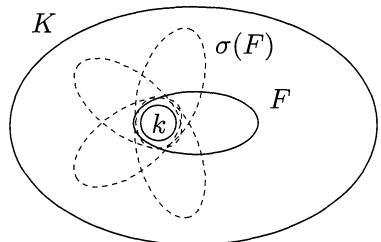
\includegraphics[width=0.45\textwidth]{figs/ch7s6-embed-nongalois.jpg}
\caption{非 Galois 扩张的多个嵌入}
\label{fig:embed-nongalois}
\end{figure}

若 $k\subseteq F$ 是 Galois 的, 所有这些像必重合:

\begin{figure}[h]
\centering
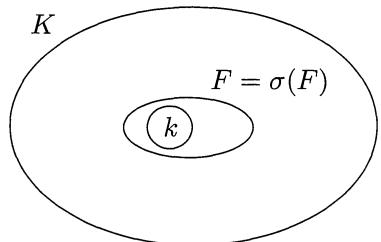
\includegraphics[width=0.45\textwidth]{figs/ch7s6-embed-galois.jpg}
\caption{Galois 扩张的嵌入具有相同的像}
\label{fig:embed-galois}
\end{figure}

当然仍可能有许多方式把 $F$ 嵌入 $K$, 但它们都有相同的像 $F$\footnote{事实上, 当 $K=\overline k$ 时, 这样的嵌入恰有 $[F:k]_s=[F:k]=|\Aut_k(F)|$ 个; 因而对所有 $K\supseteq F$ 也一样.}.

例~\ref{ex:sqrt2-extension} 末尾神秘的评注现在应该有希望清楚了\footnote{这些考虑并没有用到``可分性''; 因此, 比如在特征 $0$ 时, 它们最能传达 Galois 性的直观含义.}. $k$ 的 Galois 扩张是 $\overline{k}$ 中定义良好的子域, 被 $\overline{k}$ 在 $k$ 上的自同构保持. 将此情形与非 Galois 扩张 $\mathbb{Q}\subseteq\mathbb{Q}(\sqrt[3]{2})$ 对比, 后者在 $\overline{\mathbb{Q}}$ 中承认三个不同的嵌入. 例如, 谈论 $\mathbb{Q}(\sqrt{2})$ 与 $\mathbb{Q}(\sqrt[3]{2})$ 的``复合''作为 (比如说) $\mathbb{C}$ 的子域是没有意义的: 依据所取的 $\mathbb{Q}(\sqrt[3]{2})$ 的嵌入, 它可能是也可能不是 $\mathbb{R}$ 的子域. 但谈论两个 Galois 扩张 $k\subseteq F_{1}$, $k\subseteq F_{2}$ 的复合是有意义的, 因为 $F_{1}$ 与 $F_{2}$ 都作为 $\overline{k}$ 的子域\erratumfootnote{根据官方勘误, 原书英文此处修正单复数 (subfields of $\bar{k}$).}定义良好, 故它们的复合 $F_{1}F_{2}$ 与所取的嵌入 $F_{1}\subseteq\overline{k}$, $F_{2}\subseteq\overline{k}$ 无关.

\begin{definition}\label{def:galois-group}
若 $k\subseteq F$ 是 Galois 扩张, 相应的自同构群 $\Aut_k(F)$ 称为该扩张的 \emph{Galois 群}.
\end{definition}

重申一遍, 扩张 $\mathbb{Q}\subseteq\mathbb{Q}(\sqrt[3]{2})$ 不是 Galois 扩张: 正如我们在例~\ref{ex:cube-root-2-not-galois} 中观察到的, $\Aut_{\mathbb{Q}}(\mathbb{Q}(\sqrt[3]{2}))$ 是平凡的 (从而例如定理~\ref{thm:galois-equivalence} 的条件 (3) 不成立).

另一方面, 我们已经遇到过几个 Galois 扩张的例子: 我们在 §\ref{subsec:splitting-fields} 中看到的分裂域的例子都是 Galois 扩张. §\ref{subsec:finite-fields} 的``Galois 域'' (不出所料) 是其素子域的 Galois 扩张, 由定理~\ref{thm:finite-field-classification}. 分圆域 (§\ref{subsec:cyclotomic}) 是 $\mathbb{Q}$ 的 Galois 扩张.

Galois 扩张 $k\subseteq F$ 称为循环, 交换, 等等, 若相应的自同构群 $\Aut_k(F)$ 是循环, 交换, 等等. 例如, $\mathbb{Q}\subseteq\mathbb{Q}(\zeta_{8})$ 是一个交换但非循环的 Galois 扩张 (参见命题~\ref{prop:aut-cyclotomic} 与例~\ref{ex:splitting-x8-1-aut}).

\subsection{Galois 理论基本定理, I}\label{subsec:ft-galois-I}

Galois 理论基本定理本质上是对 Galois 扩张的 Galois 对应给出更完整的描述.

此时我们已经知道:

\begin{itemize}
\item 若 $k\subseteq F$ 是 (有限) Galois 扩张, 则存在一个反包含的双射
\[
\begin{tikzcd}[column sep=3em]
\{\text{中间域 }E:k\subseteq E\subseteq F\} \ar[r,shift left=.7ex] & \{\Aut_k(F)\text{ 的子群}\} \ar[l,shift left=.7ex]
\end{tikzcd},
\]
通过此双射, 中间域 $E$ 对应于 $\Aut_k(F)$ 的子群 $\Aut_E(F)$, 而子群 $G\subseteq\Aut_k(F)$ 对应于不动域 $F^G$.
\item 对每个中间域 $E$,
\[
[F:E]=|\Aut_E(F)|.
\]
进而 $E\subseteq F$ 也是 Galois 扩张 (习题~\ref{ex:intermediate-galois}), 并且
\[
[E:k]=|\Aut_k(F):\Aut_E(F)|;
\]
这由 Lagrange 定理 (推论~II.\ref{cor:lagrange}) 及其域论对应 (命题~\ref{prop:tower-degree}) 推出.
\item 扩张 $k\subseteq E$ 不必是 Galois 的. (再说一遍, $\mathbb{Q}(\sqrt[3]{2})$ 给出了反例, 因为它可以看成 $t^3-2$ 在 $\mathbb{Q}$ 上的分裂域中的中间域.)
\end{itemize}

Galois 对应是双射这一事实可以加强如下:

\begin{theorem}\label{thm:ft-galois-I}
设 $k\subseteq F$ 为 Galois 扩张. Galois 对应是 $k\subseteq F$ 的中间子域格与 $\Aut_k(F)$ 的子群格之间的一个反包含同构.

换言之 (采用引理~\ref{lem:galois-correspondence-inclusion} 的记号), 若 $E_1,E_2$ 是中间域, 而 $G_1,G_2$ 是 $\Aut_k(F)$ 的相应子群, 则 $E_1\cap E_2$ 对应于 $\langle G_1,G_2\rangle$, 而 $E_1E_2$ 对应于 $G_1\cap G_2$.
\end{theorem}

\begin{proof}
这由定理~\ref{thm:galois-equivalence} 与引理~\ref{lem:galois-correspondence-inclusion} 立即推出, 后者给出
\[
\Aut_{E_1E_2}(F)=G_1\cap G_2,\qquad F^{\langle G_1,G_2\rangle}=E_1\cap E_2,
\]
正是所需.
\end{proof}

\index{ziqun@子群(subgroup)!ziyouqunde@自由群的(of a free group)}在此背景下, 人们通常用``竖直''方式描绘域扩张, 并对子群采用平行的记号:
\[
\begin{tikzcd}[row sep=1.2em,column sep=4em]
F \ar[d,no head] & \{e\} \ar[d,no head] \\
E \ar[d,no head] & \Aut_E(F) \ar[d,no head] \\
k & \Aut_k(F)
\end{tikzcd}
\]

定理~\ref{thm:ft-galois-I} 的内容是: Galois 扩张 $k\subseteq F$ 的中间子域格与相应 Galois 群的子群格完全相同.

\begin{example}\label{ex:finite-field-lattice}
对有限域, 这一格的重合本质上已在推论~\ref{cor:finite-field-extension} 与命题~\ref{prop:aut-cyclic-frobenius} 中``手工''证得. 例如, 扩张 $\mathbb{F}_2\subseteq\mathbb{F}_{64}$ 是 Galois 的, 其 Galois 群是循环群 $C_6$, 由 Frobenius 自同构 $\varphi$ 生成. 这两个格是

\begin{figure}[h]
\centering
\begin{tikzcd}[row sep=1.4em,column sep=2em]
& \mathbb F_{64} \ar[dl,no head] \ar[dr,no head] & \\
\mathbb F_8 \ar[dr,no head] & & \mathbb F_4 \ar[dl,no head] \\
& \mathbb F_2 &
\end{tikzcd}
\caption{$\mathbb{F}_2\subseteq\mathbb{F}_{64}$ 的中间域格}
\label{fig:ex613-fields}
\end{figure}

\begin{figure}[h]
\centering
\begin{tikzcd}[row sep=1.4em,column sep=2em]
& \{e\} \ar[dl,no head] \ar[dr,no head] & \\
\{e,\varphi^3\} \ar[dr,no head] & & \{e,\varphi^2,\varphi^4\} \ar[dl,no head] \\
& \{e,\varphi,\varphi^2,\varphi^3,\varphi^4,\varphi^5\} &
\end{tikzcd}
\caption{$\Aut_{\mathbb{F}_2}(\mathbb{F}_{64})\cong C_6$ 的子群格}
\label{fig:ex613-groups}
\end{figure}

\end{example}

定理~\ref{thm:ft-galois-I} 常被用于``由群到域''的方向: 找出一个有限群的子群格本质上是一个组合问题, 而通过 Galois 对应它决定了相应 Galois 扩张的中间子域格.

\begin{example}\label{ex:sqrt2sqrt3-lattice}
扩张 $\mathbb{Q}(\sqrt{2},\sqrt{3})=\mathbb{Q}(\sqrt{2}+\sqrt{3})$ (在例~\ref{ex:sqrt2-sqrt3} 中研究过) 是多项式 $t^4-10t^2+1$ 的分裂域, 因而是 Galois 的. 我们已求得其 Galois 群为 $\mathbb{Z}/2\mathbb{Z}\times\mathbb{Z}/2\mathbb{Z}$; 这个群的格对我们而言已无秘密:

\begin{figure}[h]
\centering
\begin{tikzcd}[row sep=1.4em,column sep=2em]
& \langle(0,0)\rangle \ar[dl,no head] \ar[d,no head] \ar[dr,no head] & \\
\langle(1,0)\rangle \ar[dr,no head] & \langle(1,1)\rangle \ar[d,no head] & \langle(0,1)\rangle \ar[dl,no head] \\
& \mathbb Z/2\mathbb Z\times\mathbb Z/2\mathbb Z &
\end{tikzcd}
\caption{$(\mathbb{Z}/2\mathbb{Z})^2$ 的子群格}
\label{fig:ex614-groups}
\end{figure}

因此中间子域格也同样一目了然:

\begin{figure}[h]
\centering
\begin{tikzcd}[row sep=1.4em,column sep=2em]
& \mathbb Q(\sqrt2,\sqrt3) \ar[dl,no head] \ar[d,no head] \ar[dr,no head] & \\
\mathbb Q(\sqrt2) \ar[dr,no head] & \mathbb Q(\sqrt6) \ar[d,no head] & \mathbb Q(\sqrt3) \ar[dl,no head] \\
& \mathbb Q &
\end{tikzcd}
\caption{$\mathbb{Q}(\sqrt{2},\sqrt{3})$ 的中间子域格}
\label{fig:ex614-fields}
\end{figure}

(中间域由相应子群的生成元决定, 正如在例~\ref{ex:sqrt2-sqrt3} 中所见: 翻转 $\sqrt{3}\mapsto-\sqrt{3}$ 保持 $\mathbb{Q}(\sqrt{2})$ 不动, 等等.) Galois 理论告诉我们没有别的中间域了.
\end{example}

\subsection{Galois 理论基本定理, II}\label{subsec:ft-galois-II}

另一个常见的记号习惯是: 若扩张是 Galois 的, 则用相应的 Galois 群来标注该扩张:
\[
\begin{tikzcd}[row sep=1.1em,column sep=2em]
F \ar[d,no head,"\Aut_E(F)"] \ar[dd,bend right=65,no head,"\Aut_k(F)"'] \\
E \ar[d,no head] \\
k
\end{tikzcd}
\]

例~\ref{ex:cube-root-2-not-galois} 表明扩张 $k\subseteq E$ 未必是 Galois 扩张: $\mathbb{Q}(\sqrt[3]{2})$ 是 $\mathbb{Q}$ 到多项式 $t^3-2$ 的分裂域 (由定理~\ref{thm:galois-equivalence} 的第 (1) 款, 它是 Galois 的) 的中间域, 但如我们所见, 它不是 Galois 的. 该分裂域在 $\mathbb{Q}$ 上的次数为 $6$, 并且是 $\mathbb{Q}(\sqrt[3]{2})$ 的二次扩张. 这其实是典型情形: 每个有限可分扩张都可放大为一个 Galois 扩张 (习题~\ref{ex:galois-closure}).

无论如何, 在一个 Galois 扩张 $k\subseteq F$ 的中间域 $E$ 中, 基域 $k$ 在 $E$ 中的扩张是否为 Galois 扩张这个问题是理论的核心. 讨论的结果将非常漂亮, 而这或许是整个 Galois 理论基本定理中最引人注目的一部分:

\begin{theorem}\label{thm:ft-galois-II}
设 $k\subseteq F$ 为 Galois 扩张, 并设 $E$ 为中间域. 则 $k\subseteq E$ 是 Galois 的, 当且仅当 $\Aut_E(F)$ 在 $\Aut_k(F)$ 中正规; 在此情形存在一个同构
\[
\Aut_k(E)\cong\frac{\Aut_k(F)}{\Aut_E(F)}.
\]
\end{theorem}

关于 $\mathbb{Q}\subseteq\mathbb{Q}(\sqrt[3]{2})$ 的``问题''在于: $t^3-2$ 的分裂域的自同构群是 $S_3$ (我们很快就能验证: 参见例~\ref{ex:cubic-discriminant}). 对应于 $\mathbb{Q}(\sqrt[3]{2})$ 的子群指数为 $3$; 因而 (正如我们所知, 因为我们与 $S_3$ 很熟) 它不是正规的.

Galois 群 $\Aut_k(E)$ 在 Galois 情形将同构于商 $\Aut_k(F)/\Aut_E(F)$, 这一事实不应太过令人惊讶, 因为我们已经知道在任何情形下 $[E:k]$ 都等于 $\Aut_E(F)$ 在 $\Aut_k(F)$ 中的指数, 而该指数在子群正规时等于商的阶. 一般而言, $[E:k]$ 等于 $\Aut_E(F)$ 在 $\Aut_k(F)$ 中左陪集的个数, 而值得为这些陪集——即便在 $k\subseteq E$ 最终不是 Galois 扩张时——给出一个具体的解释.

我们已经知道 $\Aut_E(F)$ 的左陪集个数等于它在 $\Aut_k(F)$ 中的指数, 从而等于 $[E:k]$, 从而等于 $[E:k]_s$ (因为 $k\subseteq E$ 是可分的, 作为可分扩张的子扩张), 因此必然存在一个双射, 介于 $g$ 跑遍 $\Aut_k(F)$ 时的左陪集 $g\Aut_E(F)$ 与 $k$ 的代数闭包中不同的嵌入 $\iota:E\to\overline{k}$ (延拓 $\mathrm{id}_k$) 之间. 我们现在要为此二集合找到一个``有意义的''双射.

固定一个嵌入 $F\subseteq\overline{k}$, 并令 $I$ 为延拓 $k$ 上恒等的嵌入 $\iota:E\hookrightarrow\overline{k}$ 之集合. 把 $k\subseteq E$ 看成一个抽象扩张, 而非把 $E$ 等同于 $F$ 中某个特定的中间域, 是个好主意; 我们能够把 $E$ 看成扩张 $k\subseteq F$ 的中间域这一事实, 仅仅意味着对某个 $\iota\in I$ 有 $\iota(E)\subseteq F$.

如下一般性的观察使情形大为清晰:

\begin{itemize}
\item 对所有 $\iota\in I$, $\iota(E)\subseteq F$.

确实, $k\subseteq E$ 是单的 (有限且可分 $\Longrightarrow$ 单, 命题~\ref{prop:finite-sep-simple}). 若 $E=k(\alpha)$, 则 $\iota$ 由 $\iota(\alpha)$ 决定, 后者必是 $\alpha$ 在 $k$ 上的极小多项式的根. 但 $k\subseteq F$ 是正规的, 并且包含此多项式的某个根 $\iota(\alpha)$; 因此 $F$ 包含所有这些根 (定义~\ref{def:normal-extension}). 也就是说, 对所有 $\iota\in I$ 有 $\iota(\alpha)\in F$, 推出对所有 $\iota\in I$ 有 $\iota(k(\alpha))\subseteq F$.
\item 令 $\iota\in I$, 并令 $g\in\Aut_k(F)$; 则 $g\circ\iota\in I$. 因此 $\Aut_k(F)$ 作用在 $I$ 上.

此处 $g\circ\iota$ 按下述方式理解: 如前所见 $\iota(E)\subseteq F$; 因而 $g$ 限制为一个同态 $\iota(E)\to F$, 而 $g\circ\iota$ 是这个同态与 $\iota$ 的复合.
\end{itemize}

此时宜回顾我们在 §II.\ref{sec:group-actions} 中 (特别是 §II.\ref{subsec:transitive-actions}) 覆盖的群作用素材. 尤其要回忆我们曾能对群在集合上的所有可迁作用进行分类 (命题~II.\ref{prop:transitive-orbits}); 这正是我们的情形:

\begin{itemize}
\item $\Aut_k(F)$ 在 $I$ 上的作用是可迁的.

这由``分裂域的唯一性'' (引理~\ref{lem:splitting-field-unique}) 推出. 事实上, 令 $\iota_1,\iota_2\in I$. $\iota_1(E)$, $\iota_2(E)$ 都包含 $k$, 而 $F$ 是 $k$ 上的分裂域 (定理~\ref{thm:galois-equivalence} 的第 (1) 款); 因此 $F$ 同时是 (对同一多项式) 在 $\iota_1(E)$ 与 $\iota_2(E)$ 上的分裂域. 由引理~\ref{lem:splitting-field-unique}, 存在一个自同构 $g:F\to F$ 延拓同构
\[
\iota_2\circ\iota_1^{-1}:\iota_1(E)\to\iota_2(E).
\]
于是 $g\in\Aut_k(F)$ (因为 $\iota_2\circ\iota_1^{-1}$ 在 $k$ 上限制为恒等), 而 $g$ 在 $\iota_2\circ\iota_1^{-1}$ 上的限制恰恰意味着 $g\circ\iota_1=\iota_2$.
\end{itemize}

现在选取一个 $\iota\in I$, 并用它把 $E$ 等同于 $k\subseteq F$ 的一个中间域. 于是 $\Aut_E(F)=\Aut_{\iota(E)}(F)$ 是 $\Aut_k(F)$ 中那些在 $E=\iota(E)$ 上限制为恒等的元素组成的子群, 亦即 $\iota$ 的稳定子群.

\begin{itemize}
\item 作为 $\Aut_k(F)$-集合, $I$ 同构于 $\Aut_E(F)$ 在 $\Aut_k(F)$ 中左陪集的集合.
\end{itemize}

至此, 这由命题~II.\ref{prop:transitive-orbits} 立即推出.

如所承诺, 我们为这两个集合找到了一个有意义的双射, ``解释''了等式
\[
[E:k]=[E:k]_s=|I|=[\Aut_k(F):\Aut_E(F)],
\]
我们此前已由数值考虑 (即 Lagrange 定理; 参见 §\ref{subsec:ft-galois-I} 的开头) 发现. 进一步, 我们现在可以证明定理~\ref{thm:ft-galois-II} 了.

\begin{proof}[定理~\ref{thm:ft-galois-II} 的证明]
如上所观察, $\Aut_k(F)$ 在 $\iota\in I$ 上的稳定子等于 $\Aut_{\iota(E)}(F)$. 由命题~II.\ref{prop:stabilizer-conjugate}, 不同 $\iota$ 的稳定子彼此共轭; 若 $\Aut_E(F)$ 正规, 则推出对所有 $\iota\in I$
\[
\Aut_{\iota(E)}(F)=\Aut_E(F).
\]
这意味着对所有 $\iota\in I$ 有 $\iota(E)=E$, 因为对 Galois 扩张 $k\subseteq F$ Galois 对应是双射. 由此可知 $k\subseteq E$ 满足定理~\ref{thm:galois-equivalence} 的条件 (6); 因而是 Galois 的.

反过来, 假设 $k\subseteq E$ 是 Galois 的; 由同一条件 (6), 对所有 $\iota\in I$ 有 $\iota(E)=E$. 在 $E=\iota(E)$ 上的限制于是定义了一个同态
\[
\rho:\Aut_k(F)\longrightarrow\Aut_k(E).
\]
这个同态是满的 (因为 $\Aut_k(F)$ 在 $I$ 上的作用可迁), 而其核由那些在 $E$ 上限制为恒等的 $g\in\Aut_k(F)$ 组成, 亦即恰由 $\Aut_E(F)$ 组成. 这表明 $\Aut_E(F)$ 正规, 并且由群的``第一同构定理'' (推论~II.\ref{cor:first-iso}) 建立了所述同构. \qed
\end{proof}

\begin{remark}\label{rmk:galois-cover}
Galois 理论与拓扑中覆叠空间的理论之间有平行之处. 在此类比中, Galois 扩张对应于正则覆叠; 一个扩张的 Galois 群对应于覆叠变换群; 而定理~\ref{thm:ft-galois-II} 对应于如下事实: 正则覆叠被覆叠变换群的一个正规子群作商后仍是正则覆叠.

更一般的 (连通) 覆叠对应于更一般的代数扩张. 一个空间是单连通的, 当且仅当它不容许任何非平凡连通覆叠, 因此这个概念在域论中对应于如下条件: 一个域 $K$ 不容许任何非平凡代数扩张, 亦即 $K$ 是代数闭的. 把一个空间的基本群看成其基覆叠的覆叠变换群, 提示我们应当把代数闭包 $k\subseteq\overline{k}$ 的 Galois 群\footnote{当然, 扩张 $k\subseteq\overline k$ 一般并不是有限的, 因而需要 Galois 理论的无限版本; 参见注~\ref{rmk:infinite-galois}.} 看成域 $k$ 的``基本群''.

在代数几何中, 这个类比被发挥到其自然结论. 代数簇的覆叠映射 $X\to Y$ 决定一个域扩张 $K(Y)\subseteq K(X)$, 其中 $K(X),K(Y)$ 是``有理函数域'' (在仿射情形, 它们恰为相应坐标环的分式域; 参见习题~\ref{ex:rational-functions-localization}). 于是人们可以在不借助拓扑概念 (例如``从 $S^1$ 出发的连续映射'') 的情况下——这些概念在例如正特征时会有问题——用 Galois 理论把基本群之类的概念转移到代数几何环境中.
\end{remark}

\subsection{进一步的注记与例子}\label{subsec:galois-further}

假设 $k\subseteq F$ 与 $k\subseteq K$ 是包含在一个更大的 $k$ 的扩张中的两个有限扩张 (例如, 我们可以在 $k$ 的代数闭包中选取具体的嵌入 $F\subseteq\overline{k}$, $K\subseteq\overline{k}$). 于是我们可以考虑在此更大扩张中 $F,K$ 的复合 $FK$ (参见引理~\ref{lem:galois-correspondence-inclusion}). 很自然地要问 Galois 条件在此运算下如何表现.

\begin{proposition}\label{prop:composite-galois}
假设 $k\subseteq F$ 是 Galois 扩张, 而 $k\subseteq K$ 是任意有限扩张. 则 $K\subseteq KF$ 是 Galois 扩张, 且 $\Aut_K(KF)\cong\Aut_{F\cap K}(F)$.
\end{proposition}

图示如下:

\begin{figure}[h]
\centering
\begin{tikzcd}[row sep=1.1em,column sep=1em]
& KF \ar[dl,no head] \ar[dr,no head,"G"] & \\
F \ar[dr,no head,"G"'] & & K \ar[dl,no head] \\
& F\cap K \ar[d,no head] & \\
& k &
\end{tikzcd}
\caption{复合扩张的 Galois 群}
\label{fig:prop617-composite}
\end{figure}

\begin{proof}
由于 $k\subseteq F$ 是 Galois 的, 它是某个可分多项式 $f(x)\in k[x]\subseteq K[x]$ 的分裂域. $f(x)$ 的根在 $k$ 上生成 $F$, 因而在 $K$ 上生成 $KF$; 换言之, $KF$ 是 $f(x)$ 在 $K$ 上的分裂域, 所以 $K\subseteq KF$ 是 Galois 的.

若 $\sigma:KF\to KF$ 是一个延拓 $K$ 上 (从而在 $k$ 上) 恒等的自同构, 则 $\sigma$ 限制为一个延拓 $k$ 上恒等的同态 $F\to\sigma(F)$. 由于 $k\subseteq F$ 是 Galois 的, $\sigma(F)=F$ (定理~\ref{thm:galois-equivalence} 的 (6)). 因此, ``限制''定义了一个自然的群同态
\[
\rho:\Aut_K(KF)\longrightarrow\Aut_k(F).
\]
我们断言 $\rho$ 是单的. 确实, 依定义每个 $\sigma\in\Aut_K(KF)$ 在 $K$ 上是恒等; 若 $\sigma$ 在 $F$ 上限制为恒等, 则 $\sigma$ 在复合 $KF$ 上是恒等; 也就是说, 在 $\Aut_K(KF)$ 中 $\sigma=\mathrm{id}$.

因此 $\Aut_K(KF)$ 可以等同于 $\Aut_k(F)$ 的一个子群 $G$. 由于每个 $\sigma\in\Aut_K(KF)$ 固定 $K$, 限制 $\rho(\sigma)$ 固定 $F\cap K$; 亦即 $F^G\supseteq F\cap K$. 反过来, 设 $\alpha\in F^G$; 则 $K(\alpha)$ 在 $\Aut_K(KF)$ 的不动域中, 而由于 $K\subseteq KF$ 是 Galois 的 (定理~\ref{thm:galois-equivalence} 的条件 (4)), 此不动域就是 $K$ 本身. 也就是说, $\alpha\in K$, 从而推出 $F^G=F\cap K$. 由命题~\ref{prop:aut-fixed-field-degree}, $G=\Aut_{F\cap K}(F)$, 证毕.
\end{proof}

我们把验证如下事实留给读者: 若 $k\subseteq F$ 与 $k\subseteq K$ 都是 Galois 的, 则 $FK$ 在 $k$ 上也是 Galois 的, 并且 $F\cap K$ 也是 (习题~\ref{ex:composite-intersection-galois}).

\begin{example}\label{ex:cyclotomic-abelian}
我们曾把分圆域 $\mathbb{Q}(\zeta_n)$ 作为 $\mathbb{Q}$ 的扩张来研究; $\mathbb{Q}(\zeta_n)$ 是 $x^n-1$ 的分裂域, 因此这些扩张是 Galois 的; 我们已证明 (命题~\ref{prop:aut-cyclotomic}) $\Aut_{\mathbb{Q}}(\mathbb{Q}(\zeta_n))$ 同构于 $\mathbb{Z}/n\mathbb{Z}$ 的单位群.

现在令 $k$ 为任意特征为零的域. $x^n-1$ 在 $k$ 上的分裂域是 $k$ 与 $\mathbb{Q}(\zeta)$ 的复合 $k(\zeta)$. 由命题~\ref{prop:composite-galois}, 扩张 $k\subseteq k(\zeta)$ 是 Galois 的, 且 $\Aut_k(k(\zeta))$ 同构于 $\mathbb{Z}/n\mathbb{Z}$ 的单位群的一个子群. 特别地, 它是交换的.
\end{example}

前一个例子给出了一类重要的交换 Galois 扩张. 值得注意的是, 如果我们对基域 $k$ 施加某些限制, 就能对所有的循环 Galois 扩张进行分类.

\begin{proposition}\label{prop:kummer}
设 $k\subseteq F$ 是次数为 $m$ 的扩张. 假设 $k$ 包含一个本原 $m$ 次单位根, 且 $\Char k$ 不整除 $m$. 则 $k\subseteq F$ 是 Galois 且循环的, 当且仅当 $F=k(\delta)$, 其中 $\delta^m\in k$.
\end{proposition}

也就是说, 在关于 $k$ 的上述假设下, $k$ 的循环 Galois 扩张恰为形如 $k\subseteq k(\sqrt[m]{c})$ ($c\in k$) 的那些. 这是 Kummer 理论的一部分, 它是研究交换扩张的基本工具. 命题~\ref{prop:kummer} 将成为我们把 Galois 理论应用于多项式方程可解性的一个关键要素\footnote{我们将在 §\ref{subsec:radical-solvability} 中应用这一结果; 为方便起见, 那里将取 $\Char k=0$.}.

\begin{proof}
令 $\zeta\in k$ 为一个本原 $m$ 次单位根.

首先假设 $F=k(\delta)$, 其中 $\delta^m=c\in k$. 于是多项式 $x^m-c$ 的全部 $m$ 个根
\[
\delta,\zeta\delta,\zeta^2\delta,\ldots,\zeta^{m-1}\delta
\]
都在 $F$ 中, 并且 $F$ 由它们生成; 因此 $F$ 是此可分多项式 (因为 $\Char k$ 不整除 $m$) 在 $k$ 上的分裂域; 从而 (定理~\ref{thm:galois-equivalence} 的第 (1) 款) $k\subseteq F$ 是 Galois 的. 注意, 由于 $F=k(\delta)$ 在 $k$ 上的次数为 $m$, 且 $\delta$ 是 $x^m-c$ 的根, 故推出多项式 $x^m-c$ 是不可约的\erratumfootnote{根据官方勘误, 原书在此处补充说明: ``注意, 由于 $F=k(\delta)$ 在 $k$ 上的次数为 $m$, 且 $\delta$ 是 $x^m-c$ 的根, 故推出多项式 $x^m-c$ 是不可约的 (Note that since $F=k(\delta)$ has degree $m$ over $k$, and $\delta$ is a root of $x^m-c$, it follows that the polynomial $x^m-c$ is irreducible)''.}.

为看出 $\Aut_k(F)$ 是循环的, 注意每个 $\varphi\in\Aut_k(F)$ 由 $\varphi(\delta)$ 决定, 后者必是 $x^m-c$ 的一个根; 因此 $\varphi(\delta)=\zeta^i\delta$ 对某个 $i$ 成立, 此 $i$ 模 $m$ 确定. 这定义了 $\Aut_k(F)$ 到 $\mathbb{Z}/m\mathbb{Z}$ 的一个同构, 一如直接验证所示.

反过来, 假设 $k\subseteq F$ 是 Galois 的且 $\Aut_k(F)$ 循环, 由 $\varphi$ 生成. 自同构 $\varphi^i$ ($i=0,\ldots,m-1$) 两两不同; 因此它们在 $F$ 上线性无关 (习题~\ref{ex:aut-linearly-independent}). 于是存在 $\alpha\in F$ 使得\footnote{这个表达式称为 Lagrange 预解式.}
\[
\delta:=\alpha+\zeta^{-1}\varphi(\alpha)+\cdots+\zeta^{-(m-2)}\varphi^{m-2}(\alpha)+\zeta^{-(m-1)}\varphi^{m-1}(\alpha)\neq 0.
\]
注意
\[
\varphi(\delta)=\varphi(\alpha)+\zeta^{-1}\varphi^2(\alpha)+\cdots+\zeta^{-(m-2)}\varphi^{m-1}(\alpha)+\zeta^{-(m-1)}\alpha=\zeta\delta
\]
(因为 $\zeta\in k$, 故 $\varphi(\zeta)=\zeta$). 这意味着 $\delta$ 不被 $\Aut_k(F)$ 的任何非单位元固定; 也就是说, $\Aut_{k(\delta)}(F)=\{e\}$; 也就是说, $k(\delta)=F$. 进一步,
\[
\varphi(\delta^m)=(\varphi(\delta))^m=\zeta^m\delta^m=\delta^m;
\]
也就是说, $\delta^m$ 被 $\varphi$ 固定, 从而被整个 $\Aut_k(F)$ 固定. 由于 $k\subseteq F$ 是 Galois 的, 这推出 $\delta^m\in k$ (定理~\ref{thm:galois-equivalence} 的条件 (4)). 也就是说, $\delta$ 满足所述条件.
\end{proof}

\subsection*{习题}
\phantomsection
\addcontentsline{toc}{subsection}{习题}

\begin{prob}\label{ex:galois-ft-lemma}
证明引理~\ref{lem:galois-correspondence-inclusion}. [§\ref{subsec:galois-correspondence}]
\end{prob}

\begin{prob}\label{ex:quadratic-galois}
证明特征不为 $2$ 的域的二次扩张是 Galois 的.
\end{prob}

\begin{prob}\label{ex:intermediate-galois}
$\triangleright$ 设 $k\subseteq F$ 为 Galois 扩张, 并设 $E$ 为中间域. 证明 $E\subseteq F$ 是 Galois 扩张. [§\ref{subsec:ft-galois-I}]
\end{prob}

\begin{prob}\label{ex:galois-closure}
$\triangleright$ 设 $k\subseteq E$ 为有限可分扩张. 证明 $E$ 可以等同于 $k$ 的某个 Galois 扩张 $k\subseteq F$ 的中间域.

事实上, 证明存在最小的这样的扩张 $k\subseteq F$, 其意义是: 若 $k\subseteq E\subseteq K$, 其中 $k\subseteq K$ 为 Galois 的, 则存在 $F$ 到 $K$ 的一个嵌入, 它在 $E$ 上是恒等. (扩张 $k\subseteq F$ 是扩张 $k\subseteq E$ 的 Galois 闭包. 它在同构意义下显然唯一确定.) [§\ref{subsec:ft-galois-II}, \ref{ex:simple-gen-aut}]
\end{prob}

\begin{prob}\label{ex:simple-gen-aut}
我们已证明 (命题~\ref{prop:finite-sep-simple}) 所有有限可分扩张 $k\subseteq E$ 都是单的. 设 $k\subseteq F$ 是 $k\subseteq E$ 的一个 Galois 闭包 (习题~\ref{ex:galois-closure}). 对 $\alpha\in E$, 证明 $E=k(\alpha)$ 当且仅当 $\alpha$ 被所有 $\sigma\in\Aut_k(F)\setminus\Aut_E(F)$ 移动.
\end{prob}

\begin{prob}\label{ex:sqrt2sqrt2-galois}
$\bullet$ 证明 $\mathbb{Q}\subseteq\mathbb{Q}(\sqrt{2+\sqrt{2}})$ 是 Galois 的, 且具有循环 Galois 群. (参见习题~\ref{ex:xi-sqrt2-sqrt2}.)

$\bullet$ 证明 $\mathbb{Q}\subseteq\mathbb{Q}(\sqrt{3+\sqrt{5}})$ 是 Galois 的, 且其 Galois 群同构于 $(\mathbb{Z}/2\mathbb{Z})\times(\mathbb{Z}/2\mathbb{Z})$.

$\bullet$ 证明 $\mathbb{Q}\subseteq\mathbb{Q}(\sqrt{1+\sqrt{2}})$ 不是 Galois 的, 并计算其 Galois 闭包 $\mathbb{Q}\subseteq F$. 证明 $\Aut_{\mathbb{Q}}(F)\cong D_8$. (利用习题~IV.\ref{ex:order-8}.)
\end{prob}

\begin{prob}\label{ex:finite-field-galois-degree}
设 $p>0$ 为素数, 并设 $d\mid e$ 为正整数, 于是存在扩张 $F_{p^d}\subseteq F_{p^e}$. 证明 $\Aut_{F_{p^d}}F_{p^e}$ 是循环的, 并描述这个群的一个生成元. (这推广了命题~\ref{prop:aut-cyclic-frobenius}; 用 Galois 理论.)
\end{prob}

\begin{prob}\label{ex:prime-degree-galois}
设 $k\subseteq F$ 为次数 $n$ 的 Galois 扩张, 并设 $E$ 为中间域. 假设 $[E:k]$ 是整除 $n$ 的最小素数. 证明 $k\subseteq E$ 是 Galois 的.
\end{prob}

\begin{prob}\label{ex:degree75-galois}
设 $k\subseteq F$ 为次数 $75$ 的 Galois 扩张. 证明存在中间域 $E$, 满足 $k\subsetneq E\subsetneq F$, 使得扩张 $k\subseteq E$ 是 Galois 的.
\end{prob}

\begin{prob}\label{ex:normalizer-autE}
设 $k\subseteq F$ 为 Galois 扩张, 并设 $E$ 为中间域. 证明 $\Aut_E(F)$ 在 $\Aut_k(F)$ 中的正规化子恰为那些满足 $\sigma(E)\subseteq E$ 的 $\sigma\in\Aut_k(F)$ 之集合.

利用此给出如下事实的另一个证明: $E$ 在 $k$ 上 Galois, 当且仅当 $\Aut_E(F)$ 在 $\Aut_k(F)$ 中正规.
\end{prob}

\begin{prob}\label{ex:galois-transitive}
设 $k\subseteq E$ 与 $E\subseteq F$ 为 Galois 扩张.

$\bullet$ 找出一个例子说明 $k\subseteq F$ 未必是 Galois 的.

$\bullet$ 证明若每个 $\sigma\in\Aut_k(E)$ 都是某个 $\Aut_k(F)$ 的元素的限制, 则 $k\subseteq F$ 是 Galois 的.
\end{prob}

\begin{prob}\label{ex:composite-nonisomorphic}
找出两个代数扩张 $k\subseteq F$, $k\subseteq K$ 以及嵌入 $F\subseteq\overline{k}$, $\sigma_1:K\subseteq\overline{k}$, $\sigma_2:K\subseteq\overline{k}$ (延拓 $k\subseteq\overline{k}$), 使得复合 $F\sigma_1(K)$, $F\sigma_2(K)$ 不同构.

证明若 $F$ 与 $K$ 都在 $k$ 上 Galois, 则不存在这样的例子.
\end{prob}

\begin{prob}\label{ex:composite-intersection-galois}
$\triangleright$ 设 $k\subseteq F$ 与 $k\subseteq K$ 为 Galois 扩张, 并假设 $F$ 与 $K$ 是一个更大域的子域. 证明 $k\subseteq FK$ 与 $k\subseteq F\cap K$ 都是 Galois 扩张. [§\ref{subsec:galois-further}, §\ref{subsec:radical-solvability}]
\end{prob}

\begin{prob}\label{ex:aut-linearly-independent}
$\triangleright$ 设 $k\subseteq F$ 为域扩张, 并设 $\varphi_1,\ldots,\varphi_m\in\Aut_k(F)$ 为两两不同的自同构. 证明 $\varphi_1,\ldots,\varphi_m$ 在 $F$ 上线性无关. (回收/改编习题~VI.\ref{ex:distinct-eigenvectors-independent} 的提示.) [§\ref{subsec:galois-further}, \ref{ex:hilbert90-multiplicative}, §\hyperref[subsec:7.6-group-cohomology]{IX.7.6}]
\end{prob}

\begin{prob}\label{ex:norm-trace-product}
设 $k\subseteq F$ 为 Galois 扩张, 并设 $\alpha\in F$. 证明
\[
N_{k\subseteq F}(\alpha)=\prod_{\sigma\in\Aut_k(F)}\sigma(\alpha),\qquad \tr_{k\subseteq F}(\alpha)=\sum_{\sigma\in\Aut_k(F)}\sigma(\alpha).
\]
(习题~\ref{ex:norm-trace-embeddings}.)
\end{prob}

\begin{prob}\label{ex:hilbert90-multiplicative}
$\triangleright$ 设 $k\subseteq F$ 为次数 $d$ 的循环 Galois 扩张, 并设 $\varphi$ 为 $\Aut_k(F)$ 的一个生成元. 令 $\alpha\in F$ 为满足 $N_{k\subseteq F}(\alpha)=1$ 的元素.

$\bullet$ 证明自同构 $\mathrm{id}_F,\varphi,\ldots,\varphi^{d-1}$ 在 $F$ 上线性无关. (习题~\ref{ex:aut-linearly-independent}.)

$\bullet$ 证明存在 $\gamma\in F$ 使得
\[
\beta:=\gamma+\alpha\varphi(\gamma)+\alpha\varphi(\alpha)\varphi^2(\gamma)+\cdots+\alpha\varphi(\alpha)\cdots\varphi^{d-2}(\alpha)\varphi^{d-1}(\gamma)\neq 0.
\]

$\bullet$ 证明 $\alpha\varphi(\alpha)\varphi^2(\alpha)\cdots\varphi^{d-1}(\alpha)\varphi^d(\gamma)=\gamma$, 并推出 $\alpha=\beta/\varphi(\beta)$.

结合习题~\ref{ex:norm-trace-aut} 的结果, 结论是: 上述循环 Galois 扩张的元素 $\alpha$ 具有范数 $1$, 当且仅当存在 $\beta$ 使得 $\alpha=\beta/\varphi(\beta)$.

这就是 Hilbert 的定理 90 (Hilbert 的 Zahlbericht 中的第 90 个定理, 这是一份由德国数学会委托的、关于十九世纪末数论状况的报告). [\ref{ex:hilbert90-additive}, §\hyperref[subsec:7.6-group-cohomology]{IX.7.6}, IX.\ref{ex:7.18}]
\end{prob}

\begin{prob}\label{ex:hilbert90-kummer}
习题~\ref{ex:hilbert90-multiplicative} 应当让读者回想起命题~\ref{prop:kummer} 的证明, 这是有原因的. 假设 $k\subseteq F$ 是次数 $m$ 的循环 Galois 扩张, 且 $k$ 包含一个本原 $m$ 次单位根 $\zeta$. 利用 Hilbert 的定理 90 证明 $F=k(\delta)$, 其中 $\delta^m\in k$, 从而重新得到命题~\ref{prop:kummer} 所述结论的一个方向. (提示: $N_{k\subseteq F}(\zeta^{-1})$ 是什么?)

这里需要的 Hilbert 定理 90 的情形归功于 Kummer.
\end{prob}

\begin{prob}\label{ex:hilbert90-rational}
利用 Hilbert 的定理 90 找出方程 $a^2+b^2d=1$ 的所有有理根 $a,b$, 其中 $d$ 是非平方的正整数. (提示: $a^2+b^2d$ 等于 $N_{\mathbb{Q}\subseteq\mathbb{Q}(\sqrt{-d})}(a+b\sqrt{-d})$; 参见习题~\ref{ex:norm-alpha}.)
\end{prob}

\begin{prob}\label{ex:hilbert90-additive}
$\neg$ 设 $k\subseteq F$ 为次数 $d$ 的循环 Galois 扩张, 并设 $\varphi$ 为 $\Aut_k(F)$ 的一个生成元. 令 $\alpha\in F$ 为满足 $\tr_{k\subseteq F}(\alpha)=0$ 的元素. 证明 Hilbert 定理 90 的一个``加性版本'':

$\bullet$ 证明存在 $\gamma\in F$ 使得 $\tr_{k\subseteq F}(\gamma)\neq 0$.

$\bullet$ 盯着表达式
\[
\alpha\varphi(\gamma)+(\alpha+\varphi(\alpha))\varphi^2(\gamma)+\cdots+(\alpha+\varphi(\alpha)+\cdots+\varphi^{d-2}(\alpha))\varphi^{d-1}(\gamma)
\]
看.

$\bullet$ 证明存在 $\beta\in F$ 使得 $\alpha=\beta-\varphi(\beta)$.

结合习题~\ref{ex:norm-trace-aut}, 这说明上述循环 Galois 扩张的元素 $\alpha$ 具有迹 $0$, 当且仅当存在 $\beta$ 使得 $\alpha=\beta-\varphi(\beta)$. 一个应用见习题~\ref{ex:cyclic-char-p-artin-schreier}. [习题~\ref{ex:cyclic-char-p-artin-schreier}]
\end{prob}

\section{Galois 理论应用简述}
\label{sec:galois-applications}

Galois 理论是一个无处不在的工具, 应用极其广泛. 我们既没有能力也没有篇幅在这本书里对 Galois 理论的应用做一个充分的综述, 但即使本节回顾的这几个例子, 也足以让人感受到它相当大的威力.

\subsection{代数基本定理}
\label{subsec:ft-algebra}

定理~\ref{thm:ft-galois-II} 与一点点群论, 本质上就是给出代数基本定理的一个纯代数证明所需要的全部\footnote{其实我们稍微作弊了一点, 因为中间值定理也会在幕后用到. 这并不太令人意外: $\mathbb{R}$ 的完备性必须在某个地方进入证明.}, 这个证明我们早在 §V.\ref{subsec:irred-CRQ} 就许诺过了.

\begin{theorem}\label{thm:ft-algebra}
$\mathbb{C}$ 是代数闭的.
\end{theorem}

\begin{proof}
设 $f(x)\in\mathbb{C}[x]$ 为一个非常数多项式; 我们要证明 $f(x)$ 在 $\mathbb{C}$ 中有根. 注意若 $f(x)$ 在 $\mathbb{C}$ 中没有根, 则 $f(x)\overline{f(x)}\in\mathbb{R}[x]$ 也没有根 (其中 $\overline{f(x)}$ 表示把 $f(x)$ 的系数取复共轭所得的多项式); 也就是说, 我们不妨假设 $f(x)$ 有实系数. 令 $F$ 为 $f(x)$ 在 $\mathbb{R}$ 上的一个分裂域; 将 $F$ 嵌入 $\mathbb{R}$ 的一个代数闭包中 (我们``还不知道'' $\mathbb{C}$ 是代数闭的!), 并考虑扩张
\[
\mathbb{R}\subseteq F(i).
\]
这个扩张是 Galois 的: 它是多项式 $f(x)(x^2+1)$ 的无平方因子部分\footnote{即取该多项式的每个不可约因子, 其幂次恰好为 $1$. 在完美域上, 无平方因子多项式显然可分.}的分裂域. 令 $G=\Aut_{\mathbb{R}}(F(i))$.

由西罗 I (定理~IV.\ref{thm:sylow-I}), $G$ 有一个 $2$-西罗子群 $H$. 指数 $[G:H]$ 为奇数, 因此它对应于一个有限可分扩张 $\mathbb{R}\subseteq E$, 满足 $[E:\mathbb{R}]$ 为奇数. 然而, $\mathbb{R}$ 上每个奇次多项式都有实根 (习题~V.\ref{ex:odd-degree-ivt}, 它只用到初等的微积分), 由此推出 $\mathbb{R}\subseteq E$ 是平凡的 (习题~\ref{ex:no-irred-no-sep-extension}).

因此 $[G:H]=1$, 说明 $G$ 是一个 $2$-群. 由于 $\mathbb{C}=\mathbb{R}(i)\subseteq F(i)$, Galois 扩张 (也是 Galois 的) $\mathbb{C}\subseteq F(i)$ 的 Galois 群是 $G$ 的一个子群; 因此它是一个 $2$-群: $\lvert\Aut_{\mathbb{C}}(F(i))\rvert=2^n$ 对某个 $n\ge 0$.

现在回忆 (命题~IV.\ref{prop:p-subgroup-all-sizes}), 对每个素数 $p$, 阶为 $p^n$ 的群都含有阶为 $p^m$ 的子群, 其中 $0\le m\le n$. 特别地, 若 $n\ge 1$, 则 $\Aut_{\mathbb{C}}(F(i))$ 含有一个阶为 $2^{n-1}$ 的子群, 它通过 Galois 对应对应于 $\mathbb{C}$ 的一个二次扩张. 然而 $\mathbb{C}$ 没有二次扩张, 因为 $\mathbb{C}[x]$ 中不存在不可约的二次多项式 (再次见习题~\ref{ex:no-irred-no-sep-extension}).

这个矛盾说明 $n=0$; 也就是说, $\Aut_{\mathbb{C}}(F(i))$ 必然是平凡的. 这就证明了 $F(i)=\mathbb{C}$, 特别地 $\mathbb{C}$ 含有 $f(x)$ 的根.
\end{proof}

也可以把论证进一步简化, 绕过西罗定理的使用, 代价只是长度略有增加. 但是, 在第四章花了那么大力气证明西罗定理之后, 我们又何必去绕过它呢?

\subsection{正 \texorpdfstring{$n$}{n} 边形的作图}
\label{subsec:constructible-ngons}

我们最后一次回到正 $n$ 边形作图的问题. 较为简单的考虑已经给出了 $n$ 必须满足的约束条件, 正 $n$ 边形要可作图, 这些条件必不可少: 若 $n=p$ 为素数, 我们已经发现 $p-1$ 必须是 $2$ 的幂 (§\ref{subsec:famous-impossibilities}); 对任意的 $n$ 这个结果被加强为 $\varphi(n)$ 是 $2$ 的幂, 见 §\ref{subsec:cyclotomic} (而一个更明确的条件由习题~\ref{ex:regular-n-gon-constructible} 给出). 但这些全都是``否定性''的结果: 我们至今尚未证明, 如果 $\varphi(n)$ 是 $2$ 的幂, 那么正 $n$ 边形就真的可作图. 这正是 Galois 理论出场的地方.

\begin{proposition}\label{prop:constructible-tower}
设 $k\subseteq F$ 为 Galois 扩张, 并设 $[F:k]=p^r$, 其中 $p$ 为某个素数, $r\ge 0$. 则存在中间域
\[
k=E_0\subseteq E_1\subseteq E_2\subseteq\cdots\subseteq E_r=F
\]
使得对 $i=1,\ldots,r$ 有 $[E_i:E_{i-1}]=p$.
\end{proposition}

\begin{proof}
由于对 Galois 扩张 Galois 对应是双射的 (定理~\ref{thm:galois-equivalence} 的第 (5) 款), 这个结论直接从如下事实推出: 阶为 $p^r$ (其中 $p$ 为素数) 的群有一条由 $p$-子群构成的完全子群列; 例如可参见定理~IV.\ref{thm:sylow-II} 之后的讨论.
\end{proof}

\begin{theorem}\label{thm:regular-n-gon}
正 $n$ 边形可用直尺与圆规作图, 当且仅当 $\varphi(n)$ 是 $2$ 的幂.
\end{theorem}

\begin{proof}
如上所忆, 我们已经建立了 ``$\Longrightarrow$'' 方向.

对反方向, 假设对某个 $r$ 有 $\varphi(n)=2^r$. 扩张 $\mathbb{Q}\subseteq\mathbb{Q}(\zeta_n)$ 是 Galois 的 (它是分圆多项式 $\Phi_n(x)$ 的分裂域), 其阶为 $[\mathbb{Q}(\zeta_n):\mathbb{Q}]=\varphi(n)=2^r$ (命题~\ref{prop:cyclotomic-irred}). 命题~\ref{prop:constructible-tower} 表明定理~\ref{thm:constructible-quadratic} 所给出的条件得到满足, 从而 $\zeta_n$ 可作图, 如所求.
\end{proof}

例如 $\varphi(17)=16=2^4$; $\mathbb{Q}(\zeta_{17})$ 在 $\mathbb{Q}$ 上的 Galois 群同构于 $(\mathbb{Z}/17\mathbb{Z})^*$ (由命题~\ref{prop:aut-cyclotomic}), 因此 (定理~IV.\ref{thm:finite-subfield-cyclic}) 它是循环群, 阶为 $16$. $(\mathbb{Z}/17\mathbb{Z})^*$ 的一个生成元是 $[6]_{17}$; 由此可知 $\Aut_{\mathbb{Q}}(\mathbb{Q}(\zeta_{17}))$ 由自同构 $\sigma$ 生成, 其中 $\sigma$ 定义为 $\zeta_{17}\mapsto\zeta_{17}^6$. 子群
\[
\{e\}\subseteq\langle\sigma^8\rangle\subseteq\langle\sigma^4\rangle\subseteq\langle\sigma^2\rangle\subseteq\langle\sigma\rangle
\]
通过 Galois 对应对应于一列扩张
\[
\mathbb{Q}\subseteq\mathbb{Q}(\zeta_{17})^{\langle\sigma^2\rangle}\subseteq\mathbb{Q}(\zeta_{17})^{\langle\sigma^4\rangle}\subseteq\mathbb{Q}(\zeta_{17})^{\langle\sigma^8\rangle}\subseteq\mathbb{Q}(\zeta_{17}).
\]
运用我们现在所知的知识, 来看一看如何确定第一个扩张 (即 $\sigma^2$ 的固定域) 的一个生成元, 是很有教益的. 令 $\zeta=\zeta_{17}$. 作为 $\mathbb{Q}$-向量空间, $\mathbb{Q}(\zeta)$ 由 $\zeta,\zeta^2,\ldots,\zeta^{16}$ 生成. 为找出 $\sigma^2$ 的固定域, 写出一个 $\mathbb{Q}(\zeta)$ 的一般元素:
\[
\begin{aligned}&a_1\zeta+a_2\zeta^2+a_3\zeta^3+a_4\zeta^4+a_5\zeta^5+a_6\zeta^6+a_7\zeta^7+a_8\zeta^8\\
&+a_9\zeta^9+a_{10}\zeta^{10}+a_{11}\zeta^{11}+a_{12}\zeta^{12}+a_{13}\zeta^{13}+a_{14}\zeta^{14}+a_{15}\zeta^{15}+a_{16}\zeta^{16};
\end{aligned}
\]
由于 $\sigma^2(\zeta)=(\zeta^6)^6=\zeta^{36}=\zeta^2$, 它在 $\sigma^2$ 作用下的像为
\[
\begin{aligned}&a_1\zeta^2+a_2\zeta^4+a_3\zeta^6+a_4\zeta^8+a_5\zeta^{10}+a_6\zeta^{12}+a_7\zeta^{14}+a_8\zeta^{16}\\
&+a_9\zeta+a_{10}\zeta^3+a_{11}\zeta^5+a_{12}\zeta^7+a_{13}\zeta^9+a_{14}\zeta^{11}+a_{15}\zeta^{13}+a_{16}\zeta^{15}.
\end{aligned}
\]
这个元素被 $\sigma^2$ 固定, 当且仅当$a_1=a_2=a_4=a_8=a_{16}=a_{15}=a_{13}=a_9$ 且 $a_3=a_6=a_{12}=a_7=a_{14}=a_{11}=a_5=a_{10}$; 由此可知 $\sigma^2$ 的固定域由
\[
\delta_1:=\zeta+\zeta^2+\zeta^4+\zeta^8+\zeta^{16}+\zeta^{15}+\zeta^{13}+\zeta^9
\]
生成, 而同一个固定域也由
\[
\zeta^3+\zeta^6+\zeta^{12}+\zeta^7+\zeta^{14}+\zeta^{11}+\zeta^5+\zeta^{10}=-1-\delta_1
\]
生成 (记住 $\zeta$ 是 $\Phi_{17}(x)=x^{16}+\cdots+x+1$ 的根). 如图所见,

\begin{figure}[ht]
\centering
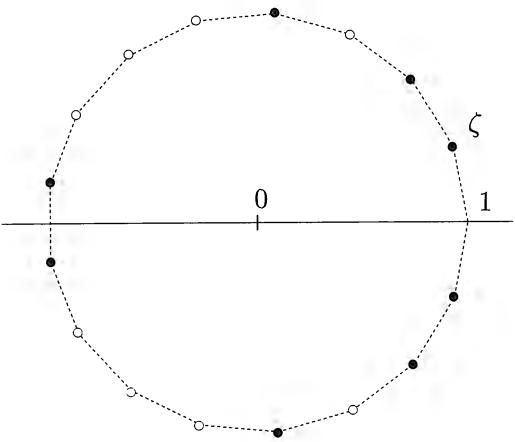
\includegraphics[width=0.55\textwidth]{figs/ch7s7-fig17roots.jpg}
\caption{正 $17$ 边形的 $17$ 次单位根. 黑点标记的根之和为 $\delta_1$; 白点标记的根之和为 $-1-\delta_1$.}
\label{fig:ch7s7-fig17roots}
\end{figure}

\noindent 黑点标记的根之和为 $\delta_1$; 白点标记的根之和为 $-1-\delta_1$. 理论告诉我们 $\delta_1$ 在 $\mathbb{Q}$ 上的次数为 $2$, 从而 $\delta_1^2$ 可写成 $1$ 与 $\delta_1$ 的有理系数线性组合. 确实, 用笔, 纸和一点耐心 (以及关系 $\zeta^{17}=1$) 可以得到
\[
\begin{aligned}\delta_1^2&=(\zeta+\zeta^2+\zeta^4+\zeta^8+\zeta^{16}+\zeta^{15}+\zeta^{13}+\zeta^9)^2\\
&=3(\zeta+\zeta^2+\zeta^4+\zeta^8+\zeta^{16}+\zeta^{15}+\zeta^{13}+\zeta^9)\\
&\quad+4(\zeta^3+\zeta^6+\zeta^{12}+\zeta^7+\zeta^{14}+\zeta^{11}+\zeta^5+\zeta^{10})+8.
\end{aligned}
\]
而第二个括号中的和等于 $-1-\delta_1$ (因为全部 $16$ 个非 $1$ 的 $17$ 次单位根之和为 $-1$); 于是
\[
\delta_1^2=3\delta_1+4(-1-\delta_1)+8=-\delta_1+4.
\]
因此 $\delta_1^2+\delta_1-4=0$. 解出 $\delta_1$ (注意 $\delta_1>0$, 因为 $0$ 右侧的黑点多于左侧的) 得
\[
\delta_1=\frac{-1+\sqrt{17}}{2}.
\]
于是我们可以轻易构造 $\delta_1$. 对其它扩张施以同样的程序可以产生 $\delta_2,\delta_3$, 最后得到 $\zeta_{17}$, 其实部就是 §\ref{subsec:famous-impossibilities} 末尾给出的那个复杂表达式.

\subsection{对称函数基本定理}
\label{subsec:sym-funcs}

设 $t_1,\ldots,t_n$ 为不定元. 多项式
\[
P_n(x):=(x-t_1)\cdots(x-t_n)\in\mathbb{Z}[t_1,\ldots,t_n][x]
\]
具有普遍性: 系数在某个 (比如说) 整环中的、次数 $n$ 的每一个首一多项式\erratumfootnote{根据官方勘误, 补充限定为首一多项式 (every monic polynomial of degree $n$).}, 都可以通过适当地指定 $t_1,\ldots,t_n$ (可能在某个更大的环中) 从 $P_n(x)$ 得到 (习题~\ref{ex:universal-poly-specialize}). 展开式
\[
P_n(x)=x^n-s_1(t_1,\ldots,t_n)x^{n-1}+s_2(t_1,\ldots,t_n)x^{n-2}-\cdots+(-1)^n s_n(t_1,\ldots,t_n)
\]
的系数 (相差一个符号) 就是 $t_1,\ldots,t_n$ 的初等对称函数. 例如, 对 $n=3$,
\[
\begin{aligned}
s_1(t_1,t_2,t_3)&=t_1+t_2+t_3,\\
s_2(t_1,t_2,t_3)&=t_1t_2+t_1t_3+t_2t_3,\\
s_3(t_1,t_2,t_3)&=t_1t_2t_3.
\end{aligned}
\]
函数 $s_i(t_1,\ldots,t_n)$ 是对称的, 意思是它们在置换 $t_1,\ldots,t_n$ 下不变 (因为 $P_n(x)$ 不变); 它们之所以是初等的, 全凭如下重要结果, 而借助 Galois 理论, 这个结果有一个特别简单的证明.

\begin{theorem}[对称函数基本定理]\label{thm:sym-funcs}
设 $K$ 为一个域, 并设 $\varphi\in K(t_1,\ldots,t_n)$. 则 $\varphi$ 是对称的, 当且仅当它是初等对称函数 $s_1,\ldots,s_n$ 的有理函数 (系数在 $K$ 中).
\end{theorem}

这里我们把 $s_i$ 无歧义地视为 $K[t_1,\ldots,t_n]$ 中的元素, 因为 $\mathbb{Z}$ 在环范畴中是初始对象.

\begin{proof}
令 $F=K(t_1,\ldots,t_n)$, 并令 $k=K(s_1,\ldots,s_n)$ 为初等对称函数在 $K$ 上生成的子域.

于是 $F$ 是可分多项式 $P_n(x)$ 在 $k$ 上的分裂域. 特别地 $k\subseteq F$ 是 Galois 扩张, 且
\[
\lvert\Aut_k(F)\rvert=[F:k]\le n!
\]
(引理~\ref{lem:splitting-field-unique}). 对称群 $S_n$ 通过置换 $t_1,\ldots,t_n$ 在 $F$ 上 (忠实地) 作用, 而这个作用在每个 $s_i$ 上都是恒等, 因为 $s_i$ 对称; 因此 $S_n$ 可以等同于 $\Aut_k(F)$ 的一个子群. 但 $\lvert S_n\rvert=n!$, 所以推出 $\Aut_k(F)=S_n$.

由于 $k\subseteq F$ 是 Galois 的, 我们得到 $k=F^{S_n}$. 这精确地说就是: 若 $\varphi\in K(t_1,\ldots,t_n)$, 则 $\varphi$ 在 $S_n$ 对 $t_1,\ldots,t_n$ 的作用下的不变性, 当且仅当 $\varphi\in k=K(s_1,\ldots,s_n)$, 这正是所要证的结论.
\end{proof}

定理~\ref{thm:sym-funcs} 的结论并不难进一步加强, 来证明每个对称多项式事实上都是初等对称函数的多项式. 注意上面证明中的推理等价于如下结果, 它值得单独记下来:

\begin{lemma}\label{lem:sym-funcs-galois}
设 $K$ 为域, $t_1,\ldots,t_n$ 为不定元, $s_1,\ldots,s_n$ 为 $t_1,\ldots,t_n$ 上的初等对称函数. 则扩张
\[
K(s_1,\ldots,s_n)\subseteq K(t_1,\ldots,t_n)
\]
是 Galois 的, 其 Galois 群为 $S_n$.
\end{lemma}

这个结果与 Cayley 定理 (定理~II.\ref{thm:cayley}) 立刻给出:

\begin{corollary}\label{cor:every-finite-group-galois}
设 $G$ 为有限群. 则存在 Galois 扩张 $k\subseteq F$ 使得 $\Aut_k(F)\cong G$.
\end{corollary}

\begin{proof}
习题~\ref{ex:every-finite-group-galois}.
\end{proof}

\index{ni Galois wenti@逆 Galois 问题(inverse Galois problem)}我们还不知道在推论~\ref{cor:every-finite-group-galois} 中能否取 $k=\mathbb{Q}$. 上面暗示的证明把 $k$ 实现为一个相当大的域, 并且完全不清楚如何从这个域``下降''到 $\mathbb{Q}$. 这就是反 Galois 问题, 一个当前研究的课题. 读者可以体会到这个问题的难度: 即使对所有的 $n$ 把 $S_n$ 实现为 $\mathbb{Q}$ 上的 Galois 群也并不容易, 尽管如下事实成立——对每个 $n$, 在 $\mathbb{Z}[x]$ 中有无穷多个 $n$ 次多项式, 其分裂域在 $\mathbb{Q}$ 上的 Galois 群为 $S_n$ (见例~\ref{ex:prime-degree-sp} 与习题~\ref{ex:prime-degree-sp-infinite} 中 $n=p$ 为素数的情形). 如果你想随身带一个好记的例子, Schur 在 1931 年证明了, ``截断指数''
\[
1+x+\frac{x^2}{2!}+\frac{x^3}{3!}+\cdots+\frac{x^n}{n!}
\]
的分裂域在 $\mathbb{Q}$ 上的 Galois 群在 $4\nmid n$ 时为 $S_n$ (在 $4\mid n$ 时为 $A_n$)\erratumfootnote{根据官方勘误, Galois 群的分支条件由 $n\neq 4$ 与 $n=4$ 修正为 $4\nmid n$ 与 $4\mid n$. }.

已知 (Shafarevich, 1954) 每个有限可解群都是 $\mathbb{Q}$ 上某个 Galois 扩张的 Galois 群.

反 Galois 问题可以重新表述为: 是否每个有限群都是 $\overline{\mathbb{Q}}$ 在 $\mathbb{Q}$ 上的 Galois 群的商群. 我们已经提到, 这个对象 (它可以诠释为 ``$\mathbb{Q}$ 的基本群''; 参见注记~\ref{rmk:galois-cover}) 是神秘且极其有趣的\footnote{据 J. S. Milne, 数学中 ``最有趣的对象'' 是 $\mathbb{Q}$ 上射影直线挖去三点 $0,1,\infty$ 后的étale基本群. 它是 $\overline{\mathbb{Q}}/\mathbb{Q}$ 的 Galois 群的一个扩张.}.

回到引理~\ref{lem:sym-funcs-galois}, 交错群 $A_n$ 在 $S_n$ 中的指数为 $2$, 因此通过 Galois 对应它对应于 $K(s_1,\ldots,s_n)$ 的一个二次扩张. 这个扩张的一个生成元很容易确定: 它必须是一个 $t_1,\ldots,t_n$ 的函数, 在所有偶置换下不变, 而在所有奇置换下不不变. 我们正是用这样的函数, 在 §IV.\ref{subsec:transpositions} 中定义了偶/奇置换:
\[
\Delta:=\prod_{1\le i<j\le n}(t_i-t_j).
\]
要看出 $\Delta$ 在 $K(s_1,\ldots,s_n)$ 上的次数为 $2$, 只需注意判别式
\[
D=\Delta^2=\prod_{1\le i<j\le n}(t_i-t_j)^2
\]
在所有置换下都不变, 因此由定理~\ref{thm:sym-funcs} 它属于域 $K(s_1,\ldots,s_n)$. 这就证明了

\begin{corollary}\label{cor:sym-funcs-an}
沿用上述记号, 扩张
\[
K(s_1,\ldots,s_n)(\sqrt{D})\subseteq K(t_1,\ldots,t_n)
\]
是 Galois 的, 其 Galois 群为 $A_n$.
\end{corollary}

\subsection{多项式方程的根式可解性}
\label{subsec:radical-solvability}

这可能是 Galois 理论最著名的一个初等工作, 也最接近 Galois 本人的原始动机.

二次方程
\[
x^2+bx+c=0
\]
 众所周知, 可由二次公式求解 (在特征 $\neq 2$ 时\footnote{在特征 $2$ 中, 可以用 ``$2$-根'' (即 Artin-Schreier 方程 $x^p-x=a$ 的根) 给出公式, 从而避开除以 $2$ 的问题; 参见习题~\ref{ex:artin-schreier-quadratic}.}):
\[
x=\frac{-b\pm\sqrt{b^2-4c}}{2}.
\]\erratumfootnote{根据官方勘误, 首一二次多项式求根公式根号内由 $b^2-4ac$ 修正为 $b^2-4c$ (因系数 $a=1$).}
对次数 $3$ 和 $4$ 的方程也存在类似但更复杂的公式 (Tartaglia/Cardano/Ferrari, 约 1540 年; 这引发了一场优先权的争论, 并退化为人身攻击). 次数 $5$ 及更高的方程则抵抗了数学家几个世纪的最佳努力. 最符合 $2,3,4$ 次情形所发生之事的雄心勃勃的目标, 是给出 ``一般的'' 多项式方程
\[
x^n+a_{n-1}x^{n-2}+\cdots+a_0=0
\]
用系数 $a_i$ 与开方等基本运算表示的解的公式. 这将是对方程的``根式''解.

然而, 这样的公式根本不存在:

\begin{theorem}\label{thm:no-radical-solution}
一般的 $5$ 次及更高次的多项式方程, 不存在根式解.
\end{theorem}

我们故意对问题所在的基域含糊其辞; 像二次公式这样的 ``公式'' 应当在任何使它有意义的域上都成立; 例如, 在二次公式的情形, 该域不应有特征 $2$. 避开这类麻烦的一个简单办法是在特征 $0$ 中工作: 这有一个主要的技术好处, 即确保多项式 $x^m-1$ (其根定义了 ``根式'') 自动可分; 参见命题~\ref{prop:kummer}. 因此, 在下文中我们将假设基域的特征为 $0$.

``一般的多项式'' 就是 §\ref{subsec:sym-funcs} 引入的 ``普遍'' 多项式 $P_n(x)$, 取在某个基域 $K$ 上: 一般的多项式
\[
x^n-s_1x^{n-1}+\cdots+(-1)^n s_n\in k[x],
\]
其中 $k=K(s_1,\ldots,s_n)$, $s_i$ 是 (``不定''的) 根 $t_1,\ldots,t_n$ 的初等对称函数. 事实上, 处理任意不可约多项式 $f(x)\in k[x]$ (在任意特征 $0$ 的域 $k$ 上) 这个更一般的情形并不更困难; 这正是我们所要做的.

用根式表示 $f(x)$ 的一个解的公式, 把 $f(x)$ 的一个根 $t_i$ 表示成如下方式从 $k$ 得到的扩张中的元素:
\[
k\subseteq k(\beta_1)\subseteq k(\beta_1,\beta_2)\subseteq\cdots\subseteq k(\beta_1,\ldots,\beta_r),
\]
其中对每个 $i=1,\ldots,r$, 对某个指数 $m_i$ 有 $\beta_i^{m_i}\in k(\beta_1,\ldots,\beta_{i-1})$.

\begin{definition}\label{def:radical-extension}
这种类型的扩张称为\emph{根式扩张}.
\end{definition}

有关根式扩张的一些事实从定义立刻得出: 例如, 若 $k\subseteq F$ 与 $k\subseteq K$ 是两个根式扩张, 且 $F,K$ 是一个更大域的子域, 则 $k\subseteq FK$ 是根式的 (习题~\ref{ex:radical-composite}). 如果基域含有所需的单位根, 则由命题~\ref{prop:kummer}, 根式扩张是循环扩张的复合. 还有,

\begin{lemma}\label{lem:sep-radical-in-galois}
每个可分的根式扩张都包含在一个 Galois 根式扩张中.
\end{lemma}

\begin{proof}
设 $k\subseteq F$ 为可分根式扩张. 特别地 $k\subseteq F$ 有限且可分, 故 $F=k(\alpha)$ 对某个 $\alpha\in F$ 成立 (命题~\ref{prop:finite-sep-simple}). 令 $p(x)$ 为 $\alpha$ 在 $k$ 上的极小多项式. $p(x)$ 在 $k$ 上的分裂域 $L$ 可以作为 $\sigma(F)$ 的复合得到, 其中 $\sigma$ 取遍 $F$ 到 $\overline{k}$ 的嵌入 (延拓 $\mathrm{id}_k$): 确实, 这个复合在 $k$ 上由所有的 $\sigma(\alpha)$ 生成, 而它们取遍 $p(x)$ 的所有根. 作为根式扩张的复合, $L$ 在 $k$ 上是根式的. 作为可分多项式的分裂域, $L$ 在 $k$ 上是 Galois 的 (定理~\ref{thm:galois-equivalence} 的第 (1) 款), 证毕.
\end{proof}

Galois 理论将允许我们把多项式 $f(x)$ 的根式可解性与关于 $f(x)$ 的分裂域的一个确切命题联系起来. 以下是这种联系的第一个形式化:

\begin{lemma}\label{lem:radical-solvable-equiv}
设 $k$ 为特征 $0$ 的域, $f(x)\in k[x]$ 为不可约多项式. 则存在一个用根式求解 $f(x)$ 的公式, 当且仅当 $f(x)$ 的分裂域包含在一个 Galois 根式扩张中.
\end{lemma}

\begin{proof}
若 $f(x)$ 的分裂域包含在一个 (无论是否 Galois 的) 根式扩张中, 则根可以写成域运算与根式的组合, 如所求.

对反方向, 假设 $f(x)$ 根式可解. 一个根 $t_i$ 的公式可以变成一个其它根 $t_j$ 的公式, 只要对 (例如) 把 $t_1$ 映到 $t_j$ 的 $\Aut_k(\overline{k})$ 的某个元素 $\sigma_i$ 应用它 (这样的自同构存在, 因为 $f(x)$ 不可约). 因此, 若一个根存在公式, 则所有根都存在公式. 所有对应的根式扩张的复合给出一个可能是更大的根式扩张, 它包含 $f(x)$ 的所有根. 从而 $f(x)$ 的分裂域包含在一个 $k$ 的根式扩张中. 由引理~\ref{lem:sep-radical-in-galois}, 这个扩张可以取为 Galois 的, 如所求.
\end{proof}

\index{duoxiangshi@多项式(polynomial)!benyuan@本原(primitive)}简而言之, 如果我们理解了多项式方程的根式可解性, 我们就理解了根式 Galois 扩张. 正如 Galois 理论的一般哲学所要求的, 我们应该力求用这些扩张的 Galois 群来刻画它们. 结果发现, 正确的条件 (在技术细节之外) 是 Galois 群应该可解.

\begin{definition}\label{def:solvable-extension}
Galois 扩张 $k\subseteq F$ 是\emph{可解的}, 如果 $\Aut_k(F)$ 是一个可解群.
\end{definition}

读者现在或许想重温 §IV.\ref{subsec:commutator}, 以回想群论中可解性的定义. (我们正接近对 ``可解'' 这一术语的解释!)

正如根式扩张分解为循环扩张的列\erratumfootnote{根据官方勘误, 原书英文此处用词由塔 (towers) 规范为序列 (sequences of cyclic extensions).}, 可解群有循环的合成因子 (命题~IV.\ref{prop:solvable-equiv}). 我们将称\footnote{警告! 这是非标准术语.}一个根式 (相应地, 可解) 扩张 $k\subseteq F$ ``含有足够多的单位根'', 如果 $k$ 含有一个公共倍数 $M$ 的 $M$ 次本原单位根, 其中 $M$ 是相应的循环因子的阶的公倍数.

\index{zugou@足够(enough)!toushe@投射(projective)}\index{zugou@足够(enough)!neishe@内射(injective)}\index{zugou@足够(enough)}\begin{lemma}\label{lem:radical-solvable-enough-roots}
设 $k\subseteq F$ 为 Galois 扩张, 且 $\Char k=0$. 只要它含有足够多的单位根, 则 $k\subseteq F$ 是根式的, 当且仅当它是可解的.
\end{lemma}

\begin{proof}
在 Galois 理论基本定理之外, 这只是命题~\ref{prop:kummer} 的一个直接推广.

确实, 假设 $k\subseteq F$ 是根式的:
\[
k\subseteq k(\beta_1)\subseteq\cdots\subseteq k(\beta_1,\ldots,\beta_r)=F,
\]
其中 $\beta_i^{m_i}\in k(\beta_1,\ldots,\beta_{i-1})$. 由假设, $k$ 对所有的 $i$ 都含有本原 $m_i$ 次单位根. 考虑 $G=\Aut_k(F)$\erratumfootnote{根据官方勘误, 明确定义群 $G=\Aut_k(F)$.} 的相应子群列:
\[
G=G_0\supseteq G_1\supseteq\cdots\supseteq G_r=\{e\},
\]
其中 $G_i=\Aut_{k(\beta_1,\ldots,\beta_i)}(F)$. 注意 $F$ 在每个中间域上都是 Galois 的. 每个扩张
\[
k(\beta_1,\ldots,\beta_{i-1})\subseteq k(\beta_1,\ldots,\beta_i)
\]
满足命题~\ref{prop:kummer} 的假设, 从而它是 Galois 且循环的. 由基本定理 (定理~\ref{thm:ft-galois-II}), 每个 $G_i$ 在之前的 $G_{i-1}$ 中正规, 且商群循环, 由此推出 $G$ 可解 (命题~IV.\ref{prop:solvable-equiv} 的 (ii)).

将上述论证反向进行, 利用命题~\ref{prop:kummer} 中的逆向蕴含, 就证明了对含有足够多单位根的可解扩张, 它们是根式的.
\end{proof}

我们如何处理可能缺失所需单位根的情况? 令人惊讶的是, 这对结论的影响相当轻微.

\begin{proposition}\label{prop:char0-solvable-radical}
设 $k$ 为特征 $0$ 的域, $k\subseteq F$ 为 Galois 扩张. 则 $k\subseteq F$ 是可解的, 当且仅当它包含在一个 Galois 根式扩张中.
\end{proposition}

命题~\ref{prop:char0-solvable-radical} 中要求特征 $0$ 是过分强了; 如同在命题~\ref{prop:kummer} 中一样, 只需要求 $\Char k$ 不整除有关的次数即可.

\begin{proof}
假设 $\Aut_k(F)$ 可解. 令 $M$ 为各循环商阶的一个公倍数, $\zeta$ 为 $\overline{k}$ (代数闭包) 中一个本原 $M$ 次单位根. 多项式 $x^M-1$ 在 $k$ 上的分裂域 $k(\zeta)$ 在 $k$ 上是 Galois 的 ($x^M-1$ 可分, 因为 $k$ 的特征为 $0$). 由命题~\ref{prop:composite-galois}, 扩张 $k(\zeta)\subseteq F(\zeta)$ 也是 Galois 的, 其 Galois 群同构于 $\Aut_{k(\zeta)\cap F}(F)$. 由于 $k(\zeta)\cap F$ 在 $k$ 上是 Galois 的 (习题~\ref{ex:composite-intersection-galois}), 这个子群正规, 由此 (推论~IV.\ref{cor:solvable-normal}) $\Aut_{k(\zeta)}(F(\zeta))$ 可解且其循环商属于 $\Aut_k(F)$ 的循环商\erratumfootnote{根据官方勘误, 原书补充并强化了商群性质推理: $\Aut_{k(\zeta)}(F(\zeta))$ 可解且其循环商属于 $\Aut_k(F)$ 的循环商; 进而 $k(\zeta)\subseteq F(\zeta)$ 含有足够多的单位根从而由引理~7.13 知是根式的.}. 特别地, $k(\zeta)\subseteq F(\zeta)$ 含有足够多的单位根, 从而由引理~\ref{lem:radical-solvable-enough-roots} 知它是根式的. $k\subseteq F(\zeta)$ 亦然, 因为 $k\subseteq k(\zeta)$ 本身是显然的根式的. 这就证明了 $k\subseteq F$ 包含在一个根式扩张中.

反过来, 假设 $k\subseteq F$ 是 Galois 的, 并包含在一个根式 Galois 扩张 $k\subseteq L$ 中. 令 $M$ 为该扩张中各循环因子阶的一个公倍数, $\zeta$ 为一个本原 $M$ 次单位根. 复合 $L(\zeta)$ 在 $k(\zeta)$ 上是 Galois 且根式的 (命题~\ref{prop:composite-galois} 与习题~\ref{ex:radical-composite}); 进一步, 它含有足够多的单位根.

由引理~\ref{lem:radical-solvable-enough-roots}, $k(\zeta)\subseteq L(\zeta)$ 是可解的. 由此推出 $k\subseteq L(\zeta)$ 可解. 确实, 这个扩张是 Galois 的 (习题~\ref{ex:composite-intersection-galois}); 把基本定理应用于
\[
k\subseteq k(\zeta)\subseteq L(\zeta)
\]
即知 $\Aut_k(k(\zeta))$ 同构于商群 $\Aut_k(L(\zeta))/\Aut_{k(\zeta)}(L(\zeta))$. 这两个群 $\Aut_{k(\zeta)}(L(\zeta))$ (如上所示) 与 $\Aut_k(k(\zeta))$ (一个 Abel 群; 参见例~\ref{ex:cyclotomic-abelian}) 都可解, 由此推出 $\Aut_k(L(\zeta))$ 可解, 如推论~IV.\ref{cor:solvable-normal} 所断言.

由于 $F$ 是中间域且在 $k$ 上 Galois, 由基本定理 $\Aut_k(F)$ 是 $\Aut_k(L(\zeta))$ 的同态像. 这说明 $\Aut_k(F)$ 是一个可解群的同态像; 从而它自身可解 (再次由推论~IV.\ref{cor:solvable-normal}), 证毕.
\end{proof}

\index{duoxiangshi@多项式(polynomial)!gen@根(radical)}我们可能忘了自己要走向何方; 不过我们已经准备好重新回到对多项式方程解的研究.

\begin{definition}\label{def:galois-group-poly}
可分多项式 $f(x)\in k[x]$ 的\emph{Galois 群} $\Gal_k(f(x))$, 是指 $f(x)$ 在 $k$ 上的分裂域的 Galois 群.\index[sym1]{22@$\Gal_k(f(x))$}
\end{definition}

\begin{corollary}\label{cor:galois-criterion}
设 $k$ 为特征 $0$ 的域, $f(x)\in k[x]$ 为不可约多项式. 则 $f(x)$ 根式可解, 当且仅当它的 Galois 群可解.
\end{corollary}

\begin{proof}
这是引理~\ref{lem:radical-solvable-equiv} 与命题~\ref{prop:char0-solvable-radical} 的直接推论.
\end{proof}

\index{Abel–Ruffini dingli@Abel–Ruffini 定理(Abel-Ruffini theorem)}推论~\ref{cor:galois-criterion} 被称为 Galois 判据. Ruffini (1799) 与 Abel (1824) 此前已经确立了, 对次数 $\ge 5$ 的方程不存在用根式表示解的一般公式 (即定理~\ref{thm:no-radical-solution}); 但正是 Galois 指出了推论~\ref{cor:galois-criterion} 所给的确切条件. 当然, 定理~\ref{thm:no-radical-solution} 立刻由 Galois 判据推出:

\begin{proof}[定理~\ref{thm:no-radical-solution} 的证明]
由引理~\ref{lem:sym-funcs-galois}, 一般的 $n$ 次多项式的 Galois 群为 $S_n$. 对 $n\ge 5$, 群 $S_n$ 不可解 (推论~IV.\ref{cor:sn-not-solvable}); 因此由推论~\ref{cor:galois-criterion} 得到结论.
\end{proof}

事实上, 我们现在还可以做得更多: 我们知道 $S_3$ 与 $S_4$ 可解 (参见习题~IV.\ref{ex:order-less-120-solvable}); 由一条带循环商的合成列, 我们原则上可以把一般的三次与四次多项式的分裂域显式地分解为根式扩张, 并由此重新得到 Tartaglia/Cardano/Ferrari 的解公式.

\subsection{多项式的 Galois 群}
\label{subsec:poly-galois-groups}

尽管 Galois 判据如此引人注目, 它本身并没有给出一个 (例如) $\mathbb{Q}$ 上 $5$ 次、且不能根式求解的多项式. 找出这样的多项式需要相当多额外的工作; 到本节末尾我们就能做到这一点.

\index{duoxiangshi@多项式(polynomial)!kefen@可分(separable)}计算多项式的 Galois 群其实是代数学家之间的一项流行运动, 要精通它所需的信息远多于读者在此能窥见的. 我们仅列出几条直接的观察.

首先, 回忆 $\Aut_k(F)$ 的一个元素必须把多项式 $f(x)\in k[x]$ 的根送到同一个多项式的根, 而如果 $f(x)$ 不可约且在 $F$ 中完全分裂, 则存在自同构把 $f(x)$ 的任一根本送到任一其它根 (命题~\ref{prop:simple-ext-iso-lift}, 引理~\ref{lem:splitting-field-unique}). 这个初等的观察可以重述如下:

\begin{lemma}\label{lem:galois-group-transitive}
设 $f(x)\in k[x]$ 为可分不可约的 $n$ 次多项式. 则 $\Gal_k(f(x))$ 在 $f(x)$ 于 $\overline{k}$ 中的根的集合上传递地作用. 特别地, $\Gal_k(f(x))$ 可以等同于对称群 $S_n$ 的一个传递子群.
\end{lemma}

当然, $S_n$ 的一个子群是传递的, 如果它对应的在 $\{1,\ldots,n\}$ 上的作用是传递的; 勤勉的读者在习题~IV.\ref{ex:transitive-subgroups} 中已经遇到过这个术语.

读者将轻易地给出引理~\ref{lem:galois-group-transitive} 在 $f(x)$ 可约情形下的类似陈述. 当然此时作用不是传递的; 如果 $f(x)$ 的各因子次数为 $n_1,\ldots,n_r$, 则 $\Gal_k(f(x))$ 包含于一个同构于 $S_{n_1}\times\cdots\times S_{n_r}$ 的 $S_n$ 的子群中.

引理~\ref{lem:galois-group-transitive} (或其 ``可约'' 的变体) 已经给出了一些信息. 例如我们看到, 可分不可约的三次多项式的 Galois 群只能是 $A_3$ 或 $S_3$, 因为它们是 $S_3$ 仅有的传递子群. 类似地, 四次不可约多项式的各种可能性相当受限: $S_4$, $A_4$, 以及同构于二面体群 $D_8$, $(\mathbb{Z}/2\mathbb{Z})\times(\mathbb{Z}/2\mathbb{Z})$, 和 $\mathbb{Z}/4\mathbb{Z}$ 的那些 (习题~\ref{ex:s4-transitive-subgroups}). 计算多项式 Galois 群的一种途径是定义一些不变量以施加进一步的限制, 从而得到判定给定多项式出现哪种可能性的算法.

我们已经遇过这些不变量中最重要的一个: 如果可分多项式 $f(x)\in k[x]$ 在其分裂域中的根为 $\alpha_1,\ldots,\alpha_n$, 则 $f(x)$ 的\emph{判别式}是元素 $D=\Delta^2$, 其中
\[
\Delta=\prod_{1\le i<j\le n}(\alpha_i-\alpha_j).
\]
根的每个置换都固定 $D$, 因此 $D$ 必须被整个 Galois 群固定; 从而 $D\in k$. 奇置换移动 $\Delta$ (若 $\Char k\neq 2$), 偶置换固定它; 因此 $\Delta$ 被 Galois 群 $G$ 固定 (也就是说 $\Delta\in k$) 当且仅当 $G\subseteq A_n$. 这就证明了

\begin{lemma}\label{lem:discriminant-an}
设 $k$ 为特征 $\neq 2$ 的域, $f(x)\in k[x]$ 为可分多项式, 判别式为 $D$. 则 $f(x)$ 的 Galois 群包含于交错群 $A_n$, 当且仅当 $D$ 是 $k$ 中的平方.
\end{lemma}

\begin{example}\label{ex:cubic-discriminant}
\index{duoxiangshi@多项式(polynomial)!henbenyuan@很本原(very primitive)}计算不可约三次多项式
\[
f(x)=x^3+ax^2+bx+c
\]
的 Galois 群, 只需引理~\ref{lem:discriminant-an} 与一个判别式的计算.

记住判别式
\[
D=a^2b^2-4a^3c-4b^3+18abc-27c^2
\]
是徒劳的; 但人们可以记住把 $x$ 平移 $a/3$ (在特征 $\neq 3$ 时) 的技巧, 其效果是消去 $x^2$ 的系数:
\[
f\!\left(x-\frac{a}{3}\right)=x^3+px+q
\]
对某个合适的 $p,q$. 这并不改变 $D$ (把所有根 $\alpha_i$ 平移同一个量对差 $\alpha_i-\alpha_j$ 没有影响), 然而
\[
D=-4p^3-27q^2
\]
更容易记住一些.

由引理~\ref{lem:discriminant-an} 与上述考虑, Galois 群在 $D$ 为平方时是 $A_3$, 否则是 $S_3$. 例如 $x^3-2$ 在 $\mathbb{Q}$ 上的 Galois 群为 $S_3$, 因为 $D=-108$ 不是 $\mathbb{Q}$ 中的平方; $x^3-3x+1$ 的判别式为 $81=9^2$, 因此它的 Galois 群为 $A_3\cong\mathbb{Z}/3\mathbb{Z}$.
\end{example}

\index{duoxiangshi@多项式(polynomial)!daifeijiaohuanbudingyuan@带非交换不定元(with noncommuting indeterminates)}读者不难找到关于四次多项式各种可能性的讨论, 以及高次多项式的详细信息. 我们仅强调如下简单的观察.

\begin{example}\label{ex:prime-degree-sp}
设 $f(x)\in\mathbb{Q}[x]$ 为 $p$ 次不可约多项式, 其中 $p$ 为素数. 假设 $f(x)$ 有 $p-2$ 个实根与 $2$ 个非实的复根. 则 $f(x)$ 的 Galois 群为 $S_p$.

确实, 复共轭诱导出分裂域的一个自同构, 并通过交换两个非实根来作用, 因此 Galois 群 $G$ (作为 $S_p$ 的子群) 含有一个对换. 另一方面, 分裂域的次数 (从而 $\lvert G\rvert$) 被 $p$ 整除, 因为它包含一个通过把任一根添加到 $\mathbb{Q}$ 得到的 $p$ 次单扩张. 由于 $p$ 为素数, 由 Cauchy 定理 (定理~IV.\ref{thm:cauchy}) $G$ 含有一个 $p$ 阶元素; $S_p$ 中仅有的 $p$ 阶元素就是 $p$-循环, 因此 $G$ 含有一个 $p$-循环. 由此 (由习题~IV.\ref{ex:sn-generated} 的一个简单变体) $G=S_p$.

例如, 多项式 $f(x)=x^5-5x-1$ 在 $\mathbb{Q}$ 上的 Galois 群为 $S_5$, 这给出了一个不能根式求解的五次式的具象例子 (习题~\ref{ex:x5-5x-1-s5}). 读者将用这个技术产生每个素数次数 $p$ 的、在 $\mathbb{Z}[x]$ 中 Galois 群为 $S_p$ 的无穷多个多项式 (习题~\ref{ex:prime-degree-sp-infinite}).
\end{example}

\subsection{Abel 群作为 \texorpdfstring{$\mathbb{Q}$}{Q} 上的 Galois 群}
\label{subsec:abelian-galois-q}

在 §\ref{subsec:sym-funcs} 提到了反 Galois 问题之后, 我们应该指出, 读者现在已处于可以证明每个有限 Abel 群都可实现为 $\mathbb{Q}$ 上某个扩张的 Galois 群的位置.

事实上, 读者可以证明一个更精确的结果: 每个有限 Abel 群都可实现为 $\mathbb{Q}$ 在分圆域 $\mathbb{Q}(\zeta_n)$ 的某个中间域的 Galois 群. 这用到一个数论事实:

对任一整数 $N$, 存在无穷多个素数 $p$ 使得 $p\equiv 1\pmod N$.

这是 Dirichlet 定理 (1837) 的一个特例; 该定理说, 若 $a,b$ 为正整数且 $\gcd(a,b)=1$, 则存在无穷多个形如 $a+nb$ ($n>0$) 的素数. 此处需要的特例 $a=1$, $b=N$ 似乎 Euler 就已经知道, 并且可以用初等方法证明 (事实上, 有一个使用分圆多项式的证明: 参见习题~\ref{ex:inf-many-primes-1-mod-n}). 假设这个事实, 论证如下:

\begin{itemize}
\item 由分类定理 (定理~IV.\ref{thm:abelian-classification}), 每个有限 Abel 群 $G$ 同构于循环群的乘积
\[
G\cong\mathbb{Z}/n_1\mathbb{Z}\times\cdots\times\mathbb{Z}/n_r\mathbb{Z}.
\]
\item 由 Dirichlet 定理, 我们可以选取互异的素数 $p_i$ 使得 $p_i\equiv 1\pmod{n_i}$.
\item 令 $n=p_1\cdots p_r$; 由中国剩余定理 (定理~V.\ref{thm:crt-general}), $(\mathbb{Z}/n\mathbb{Z})^*\cong(\mathbb{Z}/p_1\mathbb{Z})^*\times\cdots\times(\mathbb{Z}/p_r\mathbb{Z})^*$, 且右端第 $i$ 个因子是阶为 $p_i-1$ 的循环群, 是 $n_i$ 的倍数.
\item 由此 $(\mathbb{Z}/n\mathbb{Z})^*$ 含有一个子群 $H$ 使得 $G\cong(\mathbb{Z}/n\mathbb{Z})^*/H$.
\item 由于 $(\mathbb{Z}/n\mathbb{Z})^*\cong\Aut_{\mathbb{Q}}(\mathbb{Q}(\zeta_n))$ (命题~\ref{prop:aut-cyclotomic}), 且分圆域在 $\mathbb{Q}$ 上是 Galois 的, $H$ 对应于一个中间域 $F$, $\mathbb{Q}\subseteq F\subseteq\mathbb{Q}(\zeta_n)$.
\item 由于 $\Aut_{\mathbb{Q}}(\mathbb{Q}(\zeta_n))$ 是 Abel 群, $H$ 自动正规; 从而 $\mathbb{Q}\subseteq F$ 是 Galois 的, 且 $\Aut_{\mathbb{Q}}(F)\cong G$, 如所求.
\end{itemize}

于是, 对 Abel 群, ``反 Galois 问题'' 有一个容易的解.

一个更强的结果是真的: 可以证明 $\mathbb{Q}$ 的每个有限 Abel 扩张都包含于某个分圆域中. 这就是 Kronecker-Weber 定理, 可追溯到十九世纪下半叶. 这个结果的自然语境是类域论, 远远超出了本书的范围.

读者将能够验证 (习题~\ref{ex:quadratic-in-cyclotomic}), $\mathbb{Q}$ 的每个二次扩张都包含于某个分圆域中.

\subsection*{习题}
\phantomsection
\addcontentsline{toc}{subsection}{习题}

\begin{prob}\label{ex:quadratic-intermediate-10}
显式地找出扩张 $\mathbb{Q}\subseteq\mathbb{Q}(\zeta_{10})$ 的一个二次中间域的生成元.
\end{prob}

\begin{prob}\label{ex:universal-poly-specialize}
$\triangleright$ 设 $R$ 为整环, $f(x)\in R[x]$ 为 $n$ 次首一多项式\erratumfootnote{根据官方勘误, 补充限定 $f(x)$ 为首一多项式 (monic polynomial).}. 说明如何通过特化 §\ref{subsec:sym-funcs} 中定义的 ``普遍'' 多项式 $P_n(x)$ 来得到 $f(x)$. [§\ref{subsec:sym-funcs}]
\end{prob}

\begin{prob}\label{ex:elementary-symmetric-independent}
证明初等对称函数 $s_1,\ldots,s_n$ (见 §\ref{subsec:sym-funcs}) 代数无关. (提示: 利用习题~\ref{ex:transcendence-degree-tower}.)
\end{prob}

\begin{prob}\label{ex:every-finite-group-galois}
$\triangleright$ 证明每个有限群都同构于某个 Galois 扩张的自同构群. [§\ref{subsec:sym-funcs}]
\end{prob}

\begin{prob}\label{ex:radical-composite}
$\triangleright$ 设 $k\subseteq F$ 为根式扩张, $k\subseteq K$ 为任意扩张; 假设 $F$ 与 $K$ 包含在一个更大域中. 证明 $K\subseteq FK$ 是根式的. [§\ref{subsec:radical-solvability}]
\end{prob}

\begin{prob}\label{ex:cubic-splitting-Qp}
设 $f(x)\in\mathbb{Q}[x]$ 为不可约三次多项式, $\rho$ 为 $f(x)$ 的一个实根. 证明 $f(x)$ 在 $\mathbb{Q}$ 上的分裂域为 $\mathbb{Q}(\rho,\sqrt{D})$, 其中 $D$ 为 $f(x)$ 的判别式.
\end{prob}

\begin{prob}\label{ex:cubic-one-real-discriminant}
设 $f(x)\in\mathbb{Q}[x]$ 为恰有一个实根的不可约三次多项式. 证明 $f(x)$ 的判别式不是 $\mathbb{Q}$ 中的平方.
\end{prob}

\begin{prob}\label{ex:s4-transitive-subgroups}
$\triangleright$ (参见习题~IV.\ref{ex:transitive-subgroups}.) 找出 $S_4$ 的子群格, 并验证 $S_4$ 的传递子群 (同构意义下) 为 $S_4$, $A_4$, $D_8$, $\mathbb{Z}/2\mathbb{Z}\times\mathbb{Z}/2\mathbb{Z}$, 以及 $\mathbb{Z}/4\mathbb{Z}$. [§\ref{subsec:poly-galois-groups}]
\end{prob}

\begin{prob}\label{ex:galois-x4-2}
计算多项式 $x^4-2$ 的 Galois 群.
\end{prob}

\begin{prob}\label{ex:x5-5x-1-s5}
$\triangleright$ 证明多项式 $x^5-5x-1$ 恰有 $3$ 个实根 (这是一道微积分习题!) 且在 $\mathbb{Q}$ 上不可约. 证明它的 Galois 群为 $S_5$. [§\ref{subsec:poly-galois-groups}]
\end{prob}

\begin{prob}\label{ex:prime-degree-sp-infinite}
$\triangleright$ 设 $n>0$ 为整数. 注意
\[
f_n(x):=(x^2+2)\cdot x\cdot(x-2)\cdots(x-2(n-4))\cdot(x-2(n-3))
\]
有 $n-2$ 个有理根与 $2$ 个非实的复根. 证明对无穷多个整数 $q$, 多项式
\[
qf_n(x)+2\in\mathbb{Z}[x]
\]
有 $n-2$ 个实根, $2$ 个非实的复根, 且在 $\mathbb{Q}$ 上不可约. 从而对每个素数 $p$, 在 $\mathbb{Z}[x]$ 中有无穷多个 $p$ 次多项式, 其 Galois 群为 $S_p$. [§\ref{subsec:sym-funcs}, §\ref{subsec:poly-galois-groups}]
\end{prob}

\begin{prob}\label{ex:prime-degree-contains-p-cycle}
$\neg$ 设 $f(x)\in k[x]$ 为素数次数 $p$ 的可分不可约多项式, 其根 $\alpha_1,\ldots,\alpha_p$ 在分裂域 $F$ 中. 证明 $f(x)$ 的 Galois 群含有一个 $p$ 阶元素 $\sigma$, 它``循环''地穿过这些根. [\ref{ex:prime-degree-zp}]
\end{prob}

\begin{prob}\label{ex:prime-degree-zp}
$\neg$ 设 $f(x)\in k[x]$ 为素数次数 $p$ 的可分不可约多项式. 设 $\alpha$ 为 $f(x)$ 在 $\overline{k}$ 中的一个根, 并假设你可以把 $f(x)$ 的另一个根表示成 $\alpha$ 的、系数在 $k$ 中的多项式. 证明你可以把所有根都表示成 $\alpha$ 的多项式, 且 $f(x)$ 的 Galois 群为 $\mathbb{Z}/p\mathbb{Z}$. (利用习题~\ref{ex:prime-degree-contains-p-cycle}.) [\ref{ex:artin-schreier-irred}]
\end{prob}

\begin{prob}\label{ex:artin-schreier-irred}
$\neg$ 设 $k$ 为特征 $p>0$ 的域, $f(x)=x^p-x-a\in k[x]$. 假设 $f(x)$ 在 $k$ 中没有根. 证明 $f(x)$ 不可约, 且其 Galois 群为 $\mathbb{Z}/p\mathbb{Z}$. (注意若 $\alpha$ 是 $f(x)$ 的根, 则 $\alpha+1$ 也是; 利用习题~\ref{ex:irred-via-sums} 与 \ref{ex:prime-degree-zp}.)

$f(x)$ 的分裂域是 $\mathbb{F}_p$ 的一个 Artin-Schreier 扩张. [\ref{ex:artin-schreier-quadratic}]
\end{prob}

\begin{prob}\label{ex:cyclic-char-p-artin-schreier}
$\bullet$ 设 $k\subseteq F$ 为次数 $p$ 的循环 Galois 扩张, 其中 $\Char k=p>0$. 证明它是一个 Artin-Schreier 扩张. (提示: $\tr_{k\subseteq F}(1)$ 是什么? 利用 Hilbert 定理 90 的加性版本, 习题~\ref{ex:hilbert90-additive}.) [\ref{ex:hilbert90-additive}]
\end{prob}

\begin{prob}\label{ex:artin-schreier-quadratic}
$\triangleright$ 特征 $p>0$ 的域 $k$ 上的 Artin-Schreier 映射是函数
\[
x\longmapsto x^p-x.
\]
记此函数为 $\mathrm{AS}$, 并记其逆为 $\mathrm{AV}$ (它只确定到加上一个 $\mathbb{F}_p$ 的元素: 见习题~\ref{ex:artin-schreier-irred}).

对 $b\neq 0$, 用 $\mathrm{AV}$ 表示特征 $2$ 中二次方程 $x^2+bx+c=0$ 的解. (对 $b\neq 0$, 根必居于 $k$ 的一个 Artin-Schreier 扩张中, 因为此时多项式可分. 对 $b=0$ 它不可分; 在这种情形求解方程相当于把 $k$ 用 $c$ 的唯一平方根扩张.) [§\ref{subsec:radical-solvability}]
\end{prob}

\begin{prob}\label{ex:sn-galois-sn-1}
$\bullet$ 设 $f(x)\in k[x]$ 为 $k$ 上 $n$ 次可分不可约多项式, $F$ 为其分裂域. 假设 $\Aut_k(F)\cong S_n$, $a$ 为 $F$ 中 $f(x)$ 的一个根.

$\bullet$ 证明 $\Aut_{k(a)}(F)\cong S_{n-1}$.

$\bullet$ 证明 $k(a)$ 中没有真包含 $k$ 的真子域. (提示: 习题~IV.\ref{ex:s4-dihedral}.)

[\ref{ex:express-via-g}]
\end{prob}

\begin{prob}\label{ex:express-via-g}
设 $f(x)\in k[x]$ 为 $k$ 上 $n$ 次可分不可约多项式, Galois 群为 $S_n$. 令 $a$ 为 $f(x)$ 在 $\overline{k}$ 中的一个根, $g(x)\in k[x]$ 为次数 $<n$ 的任意非常数多项式. 证明 $a$ 可以表示为 $g(a)$ 的, 系数在 $k$ 中的多项式. (利用习题~\ref{ex:sn-galois-sn-1}.)
\end{prob}

\begin{prob}\label{ex:quadratic-in-cyclotomic}
$\triangleright$ 设 $d$ 为正整数.

$\bullet$ 证明多项式 $f(x)=\prod_{i=1}^n(x-\alpha_i)$ 的判别式等于 $\pm\prod_{i=1}^n f'(\alpha_i)$.

$\bullet$ 证明 $x^n-1$ 的判别式为 $\pm n^n$, 并注意它是 $\mathbb{Q}(\zeta_n)$ 中的平方.

$\bullet$ 证明 $\mathbb{Q}(\zeta_{8d})$ 包含 $d$ 与 $-d$ 的平方根.

$\bullet$ 推出 $\mathbb{Q}$ 的每个二次扩张都可嵌入某个分圆域 $\mathbb{Q}(\zeta_m)$ 中 (对某个合适的 $m$).

(这是 Kronecker-Weber 定理的一个非常特殊的情形.) [§\ref{subsec:abelian-galois-q}]
\end{prob}

% 第八章 线性代数重温 --- 中译
% 原书 pp. 483--... (Aluffi, Algebra: Chapter 0, Chapter VIII).
% 本文件进度: §8.1 Preliminaries, reprise ✅ (2026-08-31). 待续: §8.2 Tensor products and the Tor functors.

\chapter{线性代数重温}
\label{chap:linear-algebra-reprise}


% ===== 记号索引 v1 集中埋点 (页码参考原书书页; 首次出现位置待人工校对) =====
% 本章记号条目（13 条）。OCR 已做最佳校正，但部分符号字形与首次
% 出现位置仍待逐条人工复核（页码沿用原书第 699 页 Index of Notation）。
% ===== /记号索引 =====
\index[sym1]{$D^{\cate{c}}$@$D^{\cate{c}}$}
\index[sym1]{$f^*$@$f^*$}
\index[sym1]{$J$@$J$}
\index[sym1]{$K\text{-}\cate{Aff}$@$K\text{-}\cate{Aff}$}
\index[sym1]{$\Lambda:R$@$\Lambda:R$}
\index[sym1]{$\varinjlim$@$\varinjlim$}
\index[sym1]{$\varprojlim$@$\varprojlim$}
\index[sym1]{$\mathbb{Q}_p$@$\mathbb{Q}_p$}
\index[sym1]{$\Rees_R(I)$@$\Rees_R(I)$}
\index[sym1]{$\mathbb{S}^*_R$@$\mathbb{S}^*_R$}
\index[sym1]{$\tr:R$@$\tr:R$}
\index[sym1]{$z$@$z$}
\index[sym1]{$\mathbb{Z}_p$@$\mathbb{Z}_p$}
我们重新回到线性代数, 任务是研究比第六章回顾过的那些更为精细的构造. 我们的主要目标是讨论多重线性代数的若干方面, 张量积, 以及 $\Hom$ 的若干应用, 并特别把注意力放在对偶模上. 在此过程中我们还会遇到其他一些有趣的概念, 包括投射模与内射模, 以及 $\Tor$ 与 $\Ext$ 的初步.

与第六章一样, 我们将尝试处理更一般的 $R$-模情形, 仅当这能带来极大的简化或符合根深蒂固的习惯时才专门化到向量空间. 在这个一般性的层面上涵盖这些素材, 给了我们一个绝佳的借口去补充本书第一章描述过的那些预备性概念.

\section{预备知识重述}
\label{sec:lin-alg-reprise-1}

\subsection{函子}
\label{subsec:functors}

\index{fanchou@范畴(category)!Ab@Ab!xiao@小(small)}我们在本书中异常早地引入了范畴的概念, 其动机在于: 在代数的最基础处, 万有问题几乎无处不在. 我们希望, 范畴所提供的这种统一视角能帮助读者整理好我们已经遇到的那些基本构造所承载的信息.

然而, 到目前为止我们从未认真地需要``从一个范畴走到另一个范畴'', 因此我们也并不觉得非得通过更形式化地讨论这是如何做到的, 来补全对范畴的初等介绍. 细心的读者大概已经在字里行间看到过这种现象发生, 至少是以不怎么有趣的方式: 例如, 如果我们剥去一个环的乘法结构, 剩下的就是一个 Abel 群; 而如果一个域 $F$ 是一个域 $k$ 的扩张, 那么我们可以把 $F$ 看成一个 $k$-向量空间: 于是, 从 $\cate{Ring}$ 到 $\cate{Ab}$, 或者从扩张 $k$ 的范畴 $\cate{Fld}_k$ 到 $k$\dcate{-Vect}, 都有显然的``走法''. 更有趣的例子有: 环的单位群, 一个复形的同调, 一个 Galois 域扩张的自同构群 (注意后者``把箭头调转了方向''; 见下), 等等. 隐含地, 我们实际上已经遇到了这种``范畴之间的函数''的许多实例.

函子的概念把这些操作形式化了. 两个范畴 $\cate{C}$, $\cate{D}$ 之间的一个函子会把``$\cate{C}$ 的对象送到 $\cate{D}$ 的对象'', 而由于范畴携带了态射的信息, 函子也必须处理这一信息.

\begin{definition}\label{def:functor}
\index{xiebianhanzi@协变函子(covariant functor)}设 $\cate{C}$, $\cate{D}$ 为两个范畴. 一个\emph{协变函子}
\[
\mathcal{F}:\cate{C}\to\cate{D}
\]
是对每个 $A\in\Obj(\cate{C})$ 指定一个对象 $\mathcal{F}(A)\in\Obj(\cate{D})$, 并对 $\cate{C}$ 中每一对对象 $A$, $B$ 指定一个函数
\[
\Hom_{\cate{C}}(A,B)\to\Hom_{\cate{D}}(\mathcal{F}(A),\mathcal{F}(B))
\]
的赋值; 这个函数也记作 $\mathcal{F}$\footnote{这一点有点不幸, 因为这个函数的记号依赖于 $A$ 和 $B$, 但在实践中不会引起混淆. 有些作者为清晰起见写作 $\mathcal{F}_{A,B}$.}, 并且必须保持恒等态射与复合. 也就是说,
\[
\mathcal{F}(1_A)=1_{\mathcal{F}(A)}
\]
对一切 $A\in\Obj(\cate{C})$ 成立, 并且
\[
\mathcal{F}(\beta\circ\alpha)=\mathcal{F}(\beta)\circ\mathcal{F}(\alpha)
\]
对一切 $A,B,C\in\Obj(\cate{C})$, 一切 $\alpha\in\Hom_{\cate{C}}(A,B)$, 一切 $\beta\in\Hom_{\cate{C}}(B,C)$ 成立.

\index{fanbianhanzi@反变函子(contravariant functor)}一个\emph{反变函子} $\cate{C}\to\cate{D}$ 就是一个协变函子 $\cate{C}^{\op}\to\cate{D}$ (从反范畴出发).
\end{definition}

反范畴 $\cate{C}^{\op}$ 是通过``把箭头反向''从 $\cate{C}$ 得到的; 参见习题~I.\ref{ex:opposite-category}. 反变函子 $G:\cate{C}\to\cate{D}$ (即协变函子 $\cate{C}^{\op}\to\cate{D}$) 保持复合, 这意味着对一切 $A,B,C\in\Obj(\cate{C})$, 一切 $\alpha\in\Hom_{\cate{C}}(A,B)$, 一切 $\beta\in\Hom_{\cate{C}}(B,C)$:
\[
\mathcal{G}(\beta\circ\alpha)=\mathcal{G}(\alpha)\circ\mathcal{G}(\beta).
\]

形象地说,
\begin{center}
\begin{tikzcd}[column sep=large]
A \ar[r, "\alpha"] \ar[rr, "\beta\circ\alpha"', bend right=22] & B \ar[r, "\beta"] & C
\end{tikzcd}
\end{center}
被一个反变函子 $G$ 送为
\begin{center}
\begin{tikzcd}[column sep=large]
\mathcal{G}(A) & \mathcal{G}(B) \ar[l, "\mathcal{G}(\alpha)"] & \mathcal{G}(C) \ar[l, "\mathcal{G}(\beta)"'] \ar[ll, "\mathcal{G}(\beta\circ\alpha)", bend right=22]
\end{tikzcd}
\end{center}
注意复合的次序被调换了. 协变函子``保持''箭头, 也就是说, $\cate{C}$ 中每个图, 例如
\begin{center}
\begin{tikzcd}[column sep=large, row sep=large]
{} & B \ar[dr, "\beta"'] & {} \\
A \ar[ur, "\alpha_1"] \ar[rr, "\alpha_2"'] \ar[dr, "\alpha_3"'] & {} & D \\
{} & C \ar[ur, "\gamma"'] & {}
\end{tikzcd}
\qquad
\begin{tikzcd}[column sep=large, row sep=large]
{} & \mathcal{F}(B) \ar[dr, "\mathcal{F}(\beta)"'] & {} \\
\mathcal{F}(A) \ar[ur, "\mathcal{F}(\alpha_1)"] \ar[rr, "\mathcal{F}(\alpha_2)"'] \ar[dr, "\mathcal{F}(\alpha_3)"'] & {} & \mathcal{F}(D) \\
{} & \mathcal{F}(C) \ar[ur, "\mathcal{F}(\gamma)"'] & {}
\end{tikzcd}
\end{center}
都被协变函子 $\mathcal{F}:\cate{C}\to\cate{D}$ 映为一个箭头方向相同的图. 反变函子 $\mathcal{G}:\cate{C}\to\cate{D}$ ``反转''箭头:
\begin{center}
\begin{tikzcd}[column sep=large,row sep=large]
& \mathcal G(B) \ar[dl,"\mathcal G(\alpha_1)"'] & \\
\mathcal G(A) & & \mathcal G(D) \ar[ul,"\mathcal G(\beta)"'] \ar[ll,"\mathcal G(\alpha_2)"'] \ar[dl,"\mathcal G(\gamma)"] \\
& \mathcal G(C) \ar[ul,"\mathcal G(\alpha_3)"] &
\end{tikzcd}
\end{center}
在两种情形下, 交换图都被映为交换图.

在许多情形中, 反变函子被称为\emph{预层}. 于是, 范畴 $\cate{C}$ 上的一个\emph{集合预层}无非是一个反变函子 $\cate{C}\to\cate{Set}$.

如果 $\Hom_{\cate{C}}(A,B)$ 带有更多的结构, 我们可能要求函子保持这一结构. 例如, 我们已经看到: 对 $\cate{C}=R\dcate{-Mod}$ (一个环 $R$ 上的左模范畴), $\Hom_{R\text{-Mod}}(A,B)$ 自身是一个 Abel 群 (见 §III.\ref{subsec:R-Mod-hom} 末尾); 一个函子 $F:R\dcate{-Mod}\to S\dcate{-Mod}$ 如果保持这一结构, 也就是说, 如果对应的函数
\[
\Hom_{R\text{-Mod}}(A,B)\to\Hom_{S\text{-Mod}}(\mathcal{F}(A),\mathcal{F}(B))
\]
对所有 $R$-模 $A$, $B$ 都是 Abel 群的同态, 则称之为\emph{可加的}.

\subsection{函子的例子}
\label{subsec:examples-functors}

\index{fanchou@范畴(category)!Ab@Ab!zifanchou@子范畴(subcategory)}在实践中, 给一个范畴的对象指定另一个范畴的对象, 往往伴随着一个 (心理上) ``自然的'' 关于态射的对应指派, 而它显然或是协变的, 或是反变的. 我们说这个指派是\emph{函子的}, 如果它保持复合.

在 §\ref{subsec:functors} 开头提到的所有那些朴素的运算 (例如把一个环看成一个加法下的 Abel 群) 都是协变函子: 例如, 一个环同态特别地也是一个底层 Abel 群的同态, 这一事实就等于说, 给每个环标上它的底层 Abel 群定义了一个协变函子 $\cate{Ring}\to\cate{Ab}$. 由于这类函子是通过``遗忘''一个给定对象的部分结构而得到的, 它们被贴切地称为\emph{遗忘函子}.

我们已经简要地提到过几个稍具想象力的例子; 这里再把它们列一遍.

\begin{example}\label{ex:units-functor}
若 $R$ 是一个环, 我们以 $R^{*}$ 表示 $R$ 中的单位群; 每个环同态 $R\to S$ 都诱导一个群同态 $R^{*}\to S^{*}$, 并且这个指派与复合相容; 因此这个运算定义了一个协变函子 $\cate{Ring}\to\cate{Grp}$.
\end{example}

\begin{example}\label{ex:autk-contravariant}
从 Galois 域扩张到群的运算 $\Aut_k(\_)$ 是反变函子性的. 确实, 若把 $k\subseteq E\subseteq F$ 看成一个 Galois 扩张的态射 ($k\subseteq E$ 到 $k\subseteq F$), 我们就有一个对应的群同态
\[
\Aut_k(F)\to\Aut_k(E)
\]
它由限制给出: $\varphi\mapsto\varphi|_E$; 由于 Galois 条件, 后者把 $E$ 映到 $E$. 两个限制的合成仍是一个限制, 因此这个指派的确是函子性的.
\end{example}

\begin{example}\label{ex:spec-functor}
在 §III.\ref{subsec:prime-maximal-def} 中我们已经把交换环 $R$ 的\emph{谱} $\Spec R$ 定义为 $R$ 的素理想之集. 若 $R$, $S$ 是交换环, $\varphi:R\to S$ 是一个环同态, 则一个素理想 $\mathfrak{p}$ 的逆像 $\varphi^{-1}(\mathfrak{p})$ 仍是一个素理想; 于是 $\varphi$ 诱导一个集合间的函数
\[
\varphi^{*}:\Spec(S)\to\Spec(R).
\]
这个指派显然是函子性的, 因此我们可以把 $\Spec$ 看成一个从交换环范畴到 $\cate{Set}$ 的反变函子. 读者将赋予 $\Spec(R)$ 一个拓扑 (习题~\ref{ex:spec-zariski}), 使这个例子 (甚至) 更有意思.
\end{example}

\begin{example}\label{ex:presheaf-set}
若 $S$ 是一个集合, 回想 (例~I.\ref{ex:power-set-category}) 可以构造一个范畴 $\widehat{S}$, 其对象是 $S$ 的子集, 其态射对应于子集的包含. $S$ 上的一个\emph{集合预层}是一个反变函子 $\widehat{S}\to\cate{Set}$. 一个原型例子是如下函子: 它对 $U\subseteq S$ 指派从 $U$ 到一个固定集合的函数之集; 包含 $U\subseteq V$ 被映到限制 $\rho\mapsto\rho|_U$. 通过考虑更丰富的结构, 可以得到更有趣 (也更有用) 的例子. 例如, 若 $T$ 是一个拓扑空间, 可以定义一个范畴, 其对象是 $T$ 中的开集, 其态射是包含; 这就引出了拓扑空间上的预层概念. 诸如``$T$ 的开集上的 (群值的) 连续复值函数''这类标准概念, 最自然地就被看成一个在 $T$ 上的 Abel 群预层的数据. 这类具体例子常常满足额外的假设, 使它们成为\emph{层}; 但那是另一本书的主题. 在某种意义上, 研究几何的一个分支 (例如复微分几何) 就等于研究装备了一个合适的层 (例如复可微函数层) 的空间.
\end{example}

在接下来的几节中, 我们将反复用到如下一类在任何范畴上都存在的, 极为重要的函子. 设 $\cate{C}$ 是一个范畴, $X$ 是 $\cate{C}$ 的一个对象. 那么赋值
\[
A\mapsto\Hom_{\cate{C}}(X,A),\qquad A\mapsto\Hom_{\cate{C}}(A,X)
\]
分别定义了一个协变函子与一个反变函子 $\cate{C}\to\cate{Set}$. 它们分别记作 $\Hom_{\cate{C}}(X,\_)$, $\Hom_{\cate{C}}(\_,X)$. 例如, 若
\[
A\xrightarrow{\alpha}B\xrightarrow{\beta}C
\]
是 $\cate{C}$ 中的一个图, 考察
\begin{center}
\begin{tikzcd}[row sep=large,column sep=large]
A \ar[r,"\alpha"] \ar[dr,"\xi_A"'] & B \ar[r,"\beta"] \ar[d,"\xi_B"] & C \ar[dl,"\xi_C"] \\
& X &
\end{tikzcd}
\end{center}
每个 $\alpha:A\to B$ 都决定一个函数
\[
\Hom_{\cate{C}}(B,X)\to\Hom_{\cate{C}}(A,X),
\]
它把 $\xi_B$ 映为 $\xi_A:=\xi_B\circ\alpha$, 也就是说, 它要求左边的三角交换. 复合的结合律
\[
\xi_C\circ(\beta\circ\alpha)=(\xi_C\circ\beta)\circ\alpha
\]
精确表达了这个指派的\emph{反变函子性}. 函子 $\Hom_{\cate{C}}(\_,X)$ 在 $\cate{C}$ 明确时常常简记为 $h_X$.

勇敢的读者可以玩味如下事实: 这一技巧把 $\cate{C}$ 的每个对象 $X$ 联系到一个在 $\cate{C}$ 上的集合预层 $h_X$. 这就提出了自然且重要的问题, 例如如何判断一个给定的集合预层 $\mathcal{F}$ 是否事实上对某个 $\cate{C}$ 的对象 $X$ 等于 $h_X$ (这使 $\mathcal{F}$ ``可表''), 以及一个对象 $X$ 能否由对应的预层 $h_X$ 重构出来. 例如, 若 $\cate{Top}$ 是拓扑空间的范畴, $p$ 表示 $\cate{Top}$ 的终对象 (即单点拓扑空间), 那么 $h_X(p)$ 无非就是 $X$ 被看作一个集合. 因此, 在这类``几何''语境中 (例如代数几何), $h_X(A)$ 被称为``$X$ 的 $A$-点之集''; $h_X$ 就是 $X$ 的\emph{点函子}.

\subsection{两个范畴何时``等价''}
\label{subsec:equiv-categories}

\index{fanchou@范畴(category)!Ab@Ab!sanjiao@三角(triangle)}迄今为止遇到的几乎每一个``同构''概念, 归根结底都是``保持结构的双射'', 读者很自然地会期待: 那个用来辨认两个范畴的天然概念也应当从同一个模型抽取而来, 即一个把一边的对象与另一边的对象精确匹配的函子, 并保持态射的结构.

\index{fanchou@范畴(category)!Ab@Ab!daiyuji@带余积(with coproducts)}人们当然可以引入这样的概念, 但它会过分严苛. 回想, 万有问题 (也就是我们遇到的几乎每一个构造) 的解都只定义到同构为止 (命题~I.\ref{prop:initial-final-unique}). 要求一个语境中的解与另一个语境中的解精确匹配, 会是成问题的. 一个范畴中对象的结构是由它的同构类\footnote{不应当把这个观点推得太远. 把范畴中同构的对象想成``相同''固然诱人, 但这同样成问题, 而且 (就我们所知) 并不会引向一个可行的替代方案. 例如, 范畴中某些对象可能具有``更多的自同构''而其他对象没有, 如果我们简单地把范畴切成同构类, 并将所有同构强行提升为恒等态射, 这些信息就会丢失.} 充分承载的, 而``等价''的自然概念应当着眼于匹配同构类, 而非个别的对象. 态射是更本质的信息; 一个函子的优劣首先看它如何在态射上起作用.

\begin{definition}\label{def:faithful-full}
设 $\cate{C}$, $\cate{D}$ 为两个范畴. 一个协变函子 $\mathcal{F}:\cate{C}\to\cate{D}$ 是\emph{忠实的}, 如果对 $\cate{C}$ 的所有对象 $A$, $B$, 诱导出的函数
\[
\Hom_{\cate{C}}(A,B)\to\Hom_{\cate{D}}(\mathcal{F}(A),\mathcal{F}(B))
\]
是单射; 如果这个函数对所有的 $A$, $B$ 都是满射, 则称之为\emph{满的}.
\end{definition}

\emph{完全忠实的}函子 $F:\cate{C}\to\cate{D}$ 在态射上是双射, 于是很容易推出它们保持同构类: 在 $\cate{C}$ 中 $A\cong B$ 当且仅当在 $\cate{D}$ 中 $\mathcal{F}(A)\cong\mathcal{F}(B)$ (习题~\ref{ex:fully-faithful-iso}). 就所有意图与目的而言, 一个完全忠实的函子 $F:\cate{C}\to\cate{D}$ 把 $\cate{C}$ 等同于 $\cate{D}$ 的一个\emph{全的}\footnote{``全''子范畴的定义见习题~I.\ref{ex:subcategory}.} 子范畴, 即便``在对象上'' $F$ 对这个子范畴既不必是单射也不必是满射. 如下定义捕捉了这一想法:

\begin{definition}\label{def:equiv-categories}
\index{benzhimanhanzi@本质满函子(essentially surjective functor)}设 $\cate{C}$, $\cate{D}$ 为两个范畴. 一个协变函子 $\mathcal{F}:\cate{C}\to\cate{D}$ 是一个\emph{范畴等价}, 如果它是完全忠实的并且``本质满''的; 也就是说, $\mathcal{F}$ 在态射集上诱导双射, 并且对 $\cate{D}$ 的每个对象 $Y$, 都存在 $\cate{C}$ 的一个对象 $X$ 使得在 $\cate{D}$ 中 $\mathcal{F}(X)\cong Y$.

如果存在满足定义~\ref{def:equiv-categories} 中要求的函子 $F:\cate{C}\to\cate{D}$, 则称两个范畴 $\cate{C}$, $\cate{D}$ \emph{等价}. 这究竟是不是一个等价关系 (为什么它是对称的?) 绝非显然, 但事实确实如此. 实际上, 一个范畴等价 $\mathcal{F}$ 有一个``逆'' (在适当弱化的意义下): 一个函子 $\mathcal{G}:\cate{D}\to\cate{C}$, 使得从 $\mathcal{F}\circ\mathcal{G}$ 与 $\mathcal{G}\circ\mathcal{F}$ 到恒等函子都有``自然同构'' (见 §\ref{subsec:comparing-functors}). 由于我们不会太频繁地使用这些概念, 我们把这个问题留给感兴趣的读者去研究与寻找证明.
\end{definition}

\begin{example}\label{ex:matrices-fd-vect}
(参见习题~I.\ref{ex:matrix-category}.) 构造一个范畴, 取对象为非负整数, $\Hom(m,n)$ 为元素在域 $k$ 中的 $n\times m$ 矩阵之集, 复合由矩阵乘法定义 (并对没有行或列的矩阵给予适当的注意). 所得范畴等价于有限维 $k$-向量空间的范畴. 确实, 我们从前者到后者得到一个函子: 把 $n$ 送到向量空间 $k^n$ (装备标准基), 把每个矩阵送到对应的线性映射. 这个函子显然是完全忠实的, 并且它是本质满的, 因为向量空间由它们的维数分类. 这个例子使 §VI.\ref{subsec:matrices} 末尾的启发性讨论变得 (更) 精确.
\end{example}

\begin{example}\label{ex:k-aff}
回想 (定义~VII.\ref{def:coordinate-ring}) 一个域 $K$ 上的仿射代数集的坐标环是一个既约的, 交换的, 有限型的 $K$-代数. 我们可以如下定义 $K$-仿射代数集的范畴 $K\dcate{-Aff}$: 规定其对象为某个仿射 $K$-空间中的代数子集, 并定义\footnote{把 $S$ 与 $T$ 的次序颠倒是合理的: 正如读者在习题~VII.\ref{ex:polynomial-functions} 中所验证的, $K[S]$ 可以解释为 $S$ 上的``多项式函数''的 $K$-代数; 任意函数 $\varphi:S\to T$ 都决定一个函数的拉回 $K[T]\to K[S]$:\index[sym1]{34@$K\dcate{-Aff}$}
\[\begin{tikzcd}[ampersand replacement=\&,column sep=large,row sep=large]
S \ar[rr,"\varphi"] \ar[dr,"\alpha"'] \& \& T \ar[dl,"\beta"] \\
\& K \&
\end{tikzcd}\]
这里 $\alpha=\beta\circ\varphi$. 若 $\varphi$ 是代数集的态射, 这个拉回把多项式函数映到多项式函数, 并给出 $K$-代数同态 $K[T]\to K[S]$.}$\Hom_{K\dcate{-Aff}}(S,T)$ 为 $\Hom_{K\dcate{-Alg}}(K[T],K[S])$.

于是, $K\dcate{-Aff}$ 的定义使得把仿射代数集 $S$ 映到它的坐标环 $K[S]$ 的函子 $K\dcate{-Aff}^{\mathrm{op}}\to K\dcate{-Alg}$ 成为 $K\dcate{-Aff}$ 的反范畴与既约的, 交换的, 有限型 $K$-代数组成的子范畴之间的一个等价.
\end{example}

\subsection{极限与余极限}
\index{jixian@极限(limit)!toushe@投射(projective)}\index{jixian@极限(limit)!ni@逆(inverse)}\index{jixian@极限(limit)!neishe@内射(injective)}\index{jixian@极限(limit)!zhi@直(direct)}\index{jixian@极限(limit)}\label{subsec:limits-colimits}

本书一路上遇到的各种万有性质, 全都是范畴论极限这一概念的特例, 值得显式地提一下. 设 $\mathcal{F}:\cate{I}\to\cate{C}$ 是一个协变函子, 其中把 $\cate{I}$ 想成一个``指标范畴''. $\mathcal{F}$ 的\emph{极限} (如果存在) 是 $\cate{C}$ 的一个对象 $L$, 配备对 $\cate{I}$ 的所有对象 $I$ 都有的态射 $\lambda_I:L\to\mathcal{F}(I)$, 满足如下性质.

\begin{itemize}
\item 若 $\alpha:I\to J$ 是 $\cate{I}$ 中的一个态射, 则 $\lambda_J=\mathcal{F}(\alpha)\circ\lambda_I$:
\begin{center}
\begin{tikzcd}
& L \ar[dl, "\lambda_I"'] \ar[dr, "\lambda_J"] & \\
\mathcal{F}(I) \ar[rr, "\mathcal{F}(\alpha)"] & & \mathcal{F}(J)
\end{tikzcd}
\end{center}
\index{zhui@锥(cone)!hanzide@函子的(of functors)}\index{zhui@锥(cone)!yingshe@映射(map)}\index{zhui@锥(cone)}\item $L$ 关于这一性质是\emph{终的}: 也就是说, 若 $M$ 是另一个对象, 也配备满足前述要求的态射 $\mu_I$, 则存在唯一的态射 $M\to L$ 使所有相关的图交换\footnote{给定 $M$ 及这些态射的任一资料称为 $\mathcal{F}$ 的一个\emph{锥 (cone)}. 因此 $\mathcal{F}$ 的极限是一个``万有锥'': 它是 $\mathcal{F}$ 的锥的范畴 (极易定义) 中的终对象.}.
\end{itemize}

极限 $L$ (如果存在) 在同构意义下唯一, 正如每个由万有性质定义的概念一样. 它记作 $\varprojlim\mathcal{F}$. ``向左的''箭头提醒我们, $L$ 站在通过 $\mathcal{F}$ 由 $I$ 索引的 $\cate{C}$ 的所有对象``之前'' (但在同构意义下, 它是能做到这一点的``最后一个''对象). 这个概念也称为\emph{反向极限}或\emph{射影极限}.\index[sym1]{38@$\varprojlim$}

\begin{example}\label{ex:products-limit}
(乘积.) 设 $\cate{I}$ 是由两个对象 $1$, $2$ 组成的``离散范畴'', 只有恒等态射\footnote{这后一规定正是使该范畴成为``离散''范畴的原因; 参见例~I.\ref{ex:power-set-category}.}, 并设 $\mathcal{A}$ 是一个从 $\cate{I}$ 到任意范畴 $\cate{C}$ 的函子; 令 $A_1=\mathcal{A}(1)$, $A_2=\mathcal{A}(2)$ 为被 $\cate{I}$ 索引的 $\cate{C}$ 的两个对象. 那么 $\varprojlim\mathcal{A}$ 无非就是 §I.\ref{subsec:products-up} 中定义的 $A_1$ 与 $A_2$ 在 $\cate{C}$ 中的\emph{乘积}: 极限存在当且仅当 $A_1$ 与 $A_2$ 在 $\cate{C}$ 中的乘积存在.

我们可以类似地定义 $\cate{C}$ 中任意 (可能是无穷) 一族对象的乘积, 把它作为在相应的离散指标范畴上的极限, 当然, 这极限得存在才行.
\end{example}

如果指标范畴 $\cate{I}$ 带有更多的结构, 极限的概念会更有意思.

\index{denghuazi@等化子(equalizer)}\begin{example}\label{ex:equalizers-kernels}
(等化子与核.) 再次令 $\cate{I}$ 是一个有两个对象 $1$, $2$ 的范畴, 但假定态射看起来像这样:
\[
\begin{tikzcd}[column sep=large]
2 \ar[r,shift left=.7ex,"\alpha"] \ar[r,shift right=.7ex,"\beta"'] & 1
\end{tikzcd}
\]
\index{lingtaishe@零态射(zero-morphism)!zai Abel fanchouzhong@在 Abel 范畴中(in an abelian category)}也就是说, 在离散范畴上添加两个从一个对象到另一个对象的``平行''态射 $\alpha$, $\beta$. 一个函子 $K:\cate{I}\to\cate{C}$ 等价于选取 $\cate{C}$ 中的两个对象 $A_1$, $A_2$ 以及它们之间的两个平行态射. 这种函子的极限称为\emph{等化子}. 举一个具体的例子, 设 $\cate{C}=R\dcate{-Mod}$ 是某个环 $R$ 上的 $R$-模范畴; 令 $\varphi:A_2\to A_1$ 是一个同态, 并如上选取 $K$, 使得 $\mathcal{K}(\alpha)=\varphi$ 且 $\mathcal{K}(\beta)=$ 零态射. 那么 $\varprojlim K$ 无非就是 $\varphi$ 的\emph{核}, 读者可验证之 (习题~\ref{ex:kernel-verify}).
\end{example}

\begin{example}\label{ex:limits-chains}
(链上的极限.) 在另一个典型情形中, $\cate{I}$ 可能由一个全序集组成, 例如:
\[
\dots\longrightarrow 4\longrightarrow 3\longrightarrow 2\longrightarrow 1
\]
(也就是说, 对象是 $i$, 对所有正整数 $i$; 且当 $i\geq j$ 时存在唯一的态射 $i\to j$; 我们只画出了态射 $j+1\to j$). 选取 $F:\cate{I}\to\cate{C}$ 等价于对所有正整数 $i$ 选取 $\cate{C}$ 的对象 $A_i$, 以及对所有 $i\geq j$ 选取态射 $\varphi_{ji}:A_i\to A_j$, 并要求 $\varphi_{ii}=1_{A_i}$, 且对所有 $i\geq j\geq k$ 有 $\varphi_{kj}\circ\varphi_{ji}=\varphi_{ki}$. 也就是说, 选取 $F$ 等价于选取 $\cate{C}$ 中的一个图
\[
\dots\xrightarrow{\varphi_{45}}A_4\xrightarrow{\varphi_{34}}A_3\xrightarrow{\varphi_{23}}A_2\xrightarrow{\varphi_{12}}A_1.
\]
一个反向极限 $\varprojlim\mathcal{F}$ (当态射 $\varphi_{ji}$ 由语境显然时, 也可记作 $\varprojlim_i A_i$) 于是一个对象 $A$, 配备态射 $\varphi_i:A\to A_i$, 使得整个图
\begin{center}
\begin{tikzcd}[column sep=2em,row sep=large]
& & A \ar[dll,dashed] \ar[dl,"\varphi_4"'] \ar[d,"\varphi_3"'] \ar[dr,"\varphi_2"] \ar[drr,"\varphi_1"] & & \\
\cdots \ar[r,"\varphi_{45}"'] & A_4 \ar[r,"\varphi_{34}"'] & A_3 \ar[r,"\varphi_{23}"'] & A_2 \ar[r,"\varphi_{12}"'] & A_1
\end{tikzcd}
\end{center}
交换, 并且任何满足此要求的其他对象都唯一地经由 $A$ 分解.

这种极限在许多标准情形中都存在. 例如, 设 $\cate{C}=R\dcate{-Mod}$ 是固定环 $R$ 上的左模范畴, 并令 $A_i$, $\varphi_{ji}$ 如上.
\end{example}

\begin{claim}\label{claim:inverse-limit-exists}
极限 $\varprojlim_i A_i$ 在 $R\dcate{-Mod}$ 中存在.
\end{claim}

\begin{proof}
乘积 $\prod_i A_i$ 由任意序列 $(a_i)_{i>0}$ (其中 $a_i\in A_i$) 组成. 称一个序列 $(a_i)_{i>0}$ 是\emph{相干的}, 如果对所有 $i>0$ 都有 $a_i=\varphi_{i,i+1}(a_{i+1})$. 相干序列组成 $\prod_i A_i$ 的一个 $R$-子模 $A$; 典范投影限制为 $R$-模同态 $\varphi_i:A\to A_i$. 读者将验证 $A$ 是一个极限 $\varprojlim_i A_i$ (习题~\ref{ex:inverse-limit-verify}).
\end{proof}

这个例子很容易推广到由更一般的偏序集索引的族.

极限的``对偶概念''是一个函子 $F:\cate{I}\to\cate{C}$ 的\emph{余极限}. 余极限是 $\cate{C}$ 的一个对象 $C$, 配备对 $\cate{I}$ 的所有对象 $I$ 都有的态射 $\gamma_I:\mathcal{F}(I)\to C$, 使得对所有 $\alpha:I\to J$ 都有 $\gamma_I=\gamma_J\circ\mathcal{F}(\alpha)$, 并且 $C$ 关于此要求是\emph{初的}.

我们再次遇到过这一构造的好几个实例: 例如, 一个范畴中两个对象 $A_1$, $A_2$ 的余积 (如果存在) 就是在这有两个对象的离散范畴上的余极限, 正如它们的乘积是相应的极限一样. 余核是余极限, 正如核是极限一样 (参见例~\ref{ex:equalizers-kernels}).

$F$ 的余极限 (毫不意外地) 记作 $\varinjlim F$, 称为 $F$ 的\emph{正向极限}或\emph{内射极限}.\index[sym1]{37@$\varinjlim$}

再考虑全序集 $\cate{I}$ 的典型情形, 例如:
\[
1\longrightarrow 2\longrightarrow 3\longrightarrow 4\longrightarrow\dots.
\]
一个函子 $\mathcal{F}:\cate{I}\to\cate{C}$ 由对象与态射的选取组成
\[
A_1\xrightarrow{\psi_{12}}A_2\xrightarrow{\psi_{23}}A_3\xrightarrow{\psi_{34}}A_4\xrightarrow{\psi_{45}}\dots,
\]
而正向极限 $\varinjlim_i A_i$ 将是一个对象 $A$, 配备态射 $\psi_i:A_i\to A$, 使得下图交换, 并且 $A$ 关于此要求是初的:
\[
\begin{tikzcd}[column sep=2em,row sep=large]
A_1 \ar[r,"\psi_{12}"] \ar[drr,"\psi_1"'] & A_2 \ar[r,"\psi_{23}"] \ar[dr,"\psi_2"] & A_3 \ar[r,"\psi_{34}"] \ar[d,"\psi_3"] & A_4 \ar[r,"\psi_{45}"] \ar[dl,"\psi_4"] & \cdots \ar[dll,dashed] \\
& & A & &
\end{tikzcd}
\]

\begin{example}\label{ex:direct-limit-union}
若 $\cate{C}=\cate{Set}$ 且所有 $\psi_{ij}$ 都是单射, 我们就是在谈论一个``嵌套的集合序列'':
\[
A_1\subseteq A_2\subseteq A_3\subseteq A_4\subseteq\dots;
\]
这个序列的正向极限就是``无穷并'' $\bigcup_i A_i$.
\end{example}

我们已经无耻地依赖了读者的直觉并使用过这一概念, 例如在我们构造一个域的代数闭包时 (在 §VII.\ref{subsec:algebraic-closure} 中), 或者每当我们提到``有无限多个变量的''多项式环时 (例如在例~III.\ref{ex:infinitely-many-variables} 中). 更形式地, $\bigcup_i A_i$ 由对 $(i,a_i)$ 的等价类组成, 其中 $a_i\in A_i$, 且当 $i\leq j$ 时 $(i,a_i)$ 与 $(j,a_j)$ 等价当且仅当 $a_j=\psi_{ij}(a_i)$.

在 $R$-模的语境中, 可以考虑直和 $D=\bigoplus_i A_i$, 以及由对所有 $i\leq j$ 形如 $a_i-\psi_{ij}(a_i)$ 的元素生成的子模 $K\subseteq D$\erratumfootnote{此处官方勘误将原书公式中的 $a_j-\psi_{ij}(a_i)$ 更正为 $a_i-\psi_{ij}(a_i)$。} (其中每个 $A_i$ 被等同于它在 $D$ 中的像). 那么商 $D/K$ 满足所需的万有性质, 读者可验证之. 事实上, 对更一般的偏序集做这些构造也不更难 (习题~\ref{ex:colimit-verify}). 在\emph{有向集}的情形下它们更显式, 行为也更好: 偏序集 $I$ 使得对一切 $i,j\in I$ 都存在 $k\in I$ 满足 $i\leq k$, $j\leq k$.

\index{youlihanshudeya@有理函数的芽(germ of a rational function)}若干标准构造依赖于正向极限: 例如, 函数的芽 (或者更一般地, ``预层的茎'') 就是用正向极限定义的.

\subsection{比较函子}
\label{subsec:comparing-functors}

\index{fanchou@范畴(category)!Ab@Ab!daiji@带积(with products)}在把函子介绍为``范畴之间的态射''这一自然概念之后, 下一步自然要考虑``函子之间的态射''以及其他比较给定两个函子的方式. 本书不需要对这些概念做详尽的描述, 但我们要简要提几个概念与基本评注, 同样是因为它们提供了一个统一的视角.

\index{ziran@自然(natural)!bianhuan@变换(map)}\index{ziran@自然(natural)!tonggou@同构(isomorphism)}\index{ziran@自然(natural)}\begin{definition}\label{def:natural-transformation}
\index{ziranbianhuan@自然变换(natural transformation)}设 $\cate{C}$, $\cate{D}$ 为两个范畴, 并设 $F$, $G$ 为 (比如说协变的) 函子 $\cate{C}\to\cate{D}$. 一个\emph{自然变换}\footnote{更标准的记号是 $\Rightarrow$, 但它看起来太像逻辑蕴含联结词了, 我们不太喜欢, 故本书以 $\rightsquigarrow$ 表示自然变换.}$F\rightsquigarrow G$ 是对每个对象 $X\in\cate{C}$ 给出的一个态射 $\nu_X:\mathcal{F}(X)\to\mathcal{G}(X)\in\cate{D}$ 的数据, 使得对所有 $\alpha:X\to Y\in\cate{C}$ 如下图表交换:
\begin{center}
\begin{tikzcd}
\mathcal{F}(X) \ar[r, "\mathcal{F}(\alpha)"] \ar[d, "\nu_X"'] & \mathcal{F}(Y) \ar[d, "\nu_Y"] \\
\mathcal{G}(X) \ar[r, "\mathcal{G}(\alpha)"] & \mathcal{G}(Y)
\end{tikzcd}
\end{center}
一个\emph{自然同构}是一个自然变换 $\nu$, 使得对每个 $X$ 都有 $\nu_X$ 是同构.
\end{definition}

\index{Hurewicz@Hurewicz!Witold@Witold}自然变换出现在许多语境中, 例如当比较拓扑中同调与余调的不同概念时. 读者很可能遇到过 Hurewicz 同态 (从 $\pi_1$ 到 $H_1$); 它是一个自然变换. 事实上, 任何诸如``存在一个自然的 (或典范的) 同态\ldots''这样的陈述, 都很可能隐藏了两个函子之间的一个自然变换. ``自然的''这个词的技术含义, 一般来说, 与其心理上的用法是一致的.

\index{bansuihanzi@伴随函子(adjoint functors)!baochijixian/yujixian@保持极限/余极限(preserve limits/colimits)}\index{bansuihanzi@伴随函子(adjoint functors)}一个特别基本而重要的例子是\emph{伴随函子}的概念, 我们将在一个颇为非形式的层面上提及它, 而把借助自然变换使其形式化这一任务留给不屈不挠的读者. 设 $\cate{C}$, $\cate{D}$ 为两个范畴, 并设 $F:\cate{C}\to\cate{D}$, $G:\cate{D}\to\cate{C}$ 为函子. 我们说 $F$ 与 $G$ \emph{伴随} (并说 $G$ 是 $F$ 的\emph{右伴随}, $F$ 是 $G$ 的\emph{左伴随}), 如果对 $\cate{C}$ 的所有对象 $X$ 与 $\cate{D}$ 的所有对象 $Y$ 都存在自然同构
\[
\Hom_{\cate{C}}(X,\mathcal{G}(Y))\xrightarrow{\sim}\Hom_{\cate{D}}(\mathcal{F}(X),Y).
\]
(更精确地说, 应当存在一个``双函子'' $\cate{C}^{\mathrm{op}}\times\cate{D}\to\cate{Set}$ 的自然同构: $\Hom_{\cate{C}}(\_,\mathcal{G}(\_))\stackrel{\sim}{\to}\Hom_{\cate{D}}(\mathcal{F}(\_),\_)$.)

再一次, 我们一路上遇到的若干构造都可以用这些术语重述, 并且我们在本章还会遇到更多这样的情形.

\begin{example}\label{ex:free-group-adjoint}
在给定集合上构造自由群 (§II.\ref{subsec:free-groups}) 的用意在于: 给一个集合 $A$ 到一个群 $G$ 的集合函数, 与给一个从 $F(A)$ 到 $G$ 的群同态 (§II.\ref{subsec:free-universal}) 是``同一回事''. 这真正意味着: 对所有集合 $A$ 与所有群 $G$ 都有自然等同
\[
\Hom_{\cate{Set}}(A,S(G))\cong\Hom_{\cate{Grp}}(F(A),G),
\]
其中 $S(G)$ ``遗忘''了 $G$ 的群结构. 也就是说, 构造自由群的函子 $F:\cate{Set}\to\cate{Grp}$ 是遗忘函子 $S:\cate{Grp}\to\cate{Set}$ 的\emph{左伴随}.

\index{yiwanghanzi@遗忘函子(forgetful functor)!ziyouhanzideyoubansui@自由函子的右伴随(right-adjoint to free)}这当然适用于我们遇到的所有其他``自由''对象的构造: 自由函子一般说来都是遗忘函子的左伴随.
\end{example}

\index{hanzide@函子的(of functors)}于是, 有趣的函子可能是看似无害的函子的伴随. 这有技术上的好处: 有趣者的性质可以翻译成无害者的性质, 从而给出这些性质的更易的证明.

事实上, 一个函子有伴随这一事实本身就赋予该函子以方便的特性. 我们说 $F$ 是一个\emph{左伴随函子}, 如果它有一个右伴随; 而 $G$ 是一个\emph{右伴随函子}, 如果它有一个左伴随. (比如说) 右伴随函子的某些性质, 甚至可以在不知道伴随的左伴随函子是什么的情况下确立. 这里是这一现象的原型例子.

\begin{lemma}\label{lem:right-adjoint-limits}
右伴随函子与极限交换.
\end{lemma}

也就是说, 若 $\mathcal{G}:\cate{D}\to\cate{C}$ 有左伴随 $\mathcal{F}:\cate{C}\to\cate{D}$, 且 $\mathcal{A}:\cate{I}\to\cate{D}$ 是另一个函子, 则存在典范同构
\[
\mathcal{G}(\varprojlim\mathcal{A})\xrightarrow{\sim}\varprojlim(\mathcal{G}\circ\mathcal{A})
\]
(当然, 如果极限存在的话). 正如每个好的微积分学生应当立刻理解的, 这表示右伴随函子是连续的. (毋庸讳言, 左伴随函子则转而与余极限交换, 并应被称为余连续的.)

我们不会血淋淋地证明引理~\ref{lem:right-adjoint-limits}, 但我们要努力说服读者: 这类陈述比看上去容易, 它们归根结底就是对定义各个概念的万有性质做适当的应用. 相比之下, 在不借助抽象废话的情况下证明某个具体给定的函子保持乘积 (例如), 有时可能显得涉及一些``真正的''工作.

假设 $\mathcal{G}:\cate{D}\to\cate{C}$ 是 $\mathcal{F}:\cate{C}\to\cate{D}$ 的右伴随, 且 $\mathcal{A}:\cate{I}\to\cate{D}$ 是一个给定的函子. 如我们所见, $\mathcal{A}$ 的极限关于拟合进交换图是终的:
\begin{center}
\begin{tikzcd}
& \varprojlim\mathcal{A} \ar[dl,"\lambda_I"'] \ar[dr,"\lambda_J"] & \\
\mathcal{A}(I) \ar[rr, "\mathcal{A}(\alpha)"] & & \mathcal{A}(J)
\end{tikzcd}
\end{center}
(记号应无疑问). 作用 $\mathcal{G}$, 我们得到 (在 $\cate{C}$ 中的) 交换图\[
\begin{tikzcd}[column sep=large,row sep=large]
& \mathcal G(\varprojlim\mathcal A) \ar[dl,"\mathcal G(\lambda_I)"'] \ar[dr,"\mathcal G(\lambda_J)"] & \\
\mathcal G\circ\mathcal A(I) \ar[rr,"\mathcal G\circ\mathcal A(\alpha)"'] & & \mathcal G\circ\mathcal A(J)
\end{tikzcd}
\]并因此由定义 $\mathcal{G}\circ\mathcal{A}$ 的极限的万有性质得到唯一的态射 $\mathcal{G}(\varprojlim\mathcal{A})\to\varprojlim(\mathcal{G}\circ\mathcal{A})$.\[
\begin{tikzcd}[column sep=large,row sep=1.5em]
& \mathcal G(\varprojlim\mathcal A) \ar[d,dashed,"\exists!"] \ar[ddl,bend right=30] \ar[ddr,bend left=30] & \\
& \varprojlim(\mathcal G\circ\mathcal A) \ar[dl] \ar[dr] & \\
\mathcal G\circ\mathcal A(I) \ar[rr,"\mathcal G\circ\mathcal A(\alpha)"'] & & \mathcal G\circ\mathcal A(J)
\end{tikzcd}
\] 再由伴随的等同
\[
\Hom_{\cate{C}}(X,\mathcal{G}(Y))\stackrel{\sim}{\longrightarrow}\Hom_{\cate{D}}(\mathcal{F}(X),Y)
\]
出发, $\cate{C}$ 中的态射 $\varprojlim(\mathcal{G}\circ\mathcal{A})\to\mathcal{G}\circ\mathcal{A}(I)$ 决定 (在 $\cate{D}$ 中的) 态射 $\mathcal{F}(\varprojlim(\mathcal{G}\circ\mathcal{A}))\to\mathcal{A}(I)$. 由定义 $\varprojlim\mathcal{A}$ 的万有性质, 我们得到唯一的态射 $\mathcal{F}(\varprojlim(\mathcal{G}\circ\mathcal{A}))\to\varprojlim\mathcal{A}$\[
\begin{tikzcd}[column sep=large,row sep=1.5em]
& \mathcal F(\varprojlim(\mathcal G\circ\mathcal A)) \ar[d,dashed,"\exists!"] \ar[ddl,bend right=30] \ar[ddr,bend left=30] & \\
& \varprojlim\mathcal A \ar[dl] \ar[dr] & \\
\mathcal A(I) \ar[rr,"\mathcal A(\alpha)"'] & & \mathcal A(J)
\end{tikzcd}
\], 再作用伴随, 这决定了唯一的态射 $\varprojlim(\mathcal{G}\circ\mathcal{A})\to\mathcal{G}(\varprojlim\mathcal{A})$. 总之, 我们得到了自然态射
\[
\mathcal{G}(\varprojlim\mathcal{A})\to\varprojlim(\mathcal{G}\circ\mathcal{A}),\qquad\varprojlim(\mathcal{G}\circ\mathcal{A})\to\mathcal{G}(\varprojlim\mathcal{A}).
\]
容易验证这些态射的复合是恒等 (凭借构造中所援引的各种万有性质的唯一性部分), 从而完成引理~\ref{lem:right-adjoint-limits} 的验证.

这个概要所缺的, 是对每个所需图都交换这一事实的显式验证, 而这是应用上述万有性质所必需的. 读者大概会同意: 这类验证即便可能有些繁琐, 也必定是例行公事.

引理~\ref{lem:right-adjoint-limits} 推出, 例如右伴随函子保持乘积, 并且当核有意义时它们必须``保持核''.

\begin{example}\label{ex:exact-functors}
(正合函子.) 一个函子是\emph{正合的}, 如果它保持正合性, 也就是说, 它把正合序列送到正合序列. 迄今为止我们只在一个环上的模的语境中 (§III.\ref{subsec:complexes}) 研究过正合性, 因此设 $R$, $S$ 为环, 并设 $F:R\dcate{-Mod}\to S\dcate{-Mod}$ 是一个可加函子; $F$ 是正合的当且仅当每当
\[
0\longrightarrow A\xrightarrow{\varphi}B\xrightarrow{\psi}C\longrightarrow 0
\]
是一个 $R$-模的正合序列时,
\[
0\longrightarrow\mathcal{F}(A)\xrightarrow{\mathcal{F}(\varphi)}\mathcal{F}(B)\xrightarrow{\mathcal{F}(\psi)}\mathcal{F}(C)\longrightarrow 0
\]
都是一个 $S$-模的正合序列. 由此容易推出: 每个正合复形的像都是正合的 (习题~\ref{ex:exact-functor-complex}).

当一个函子不是正合的, 但却保持序列的``部分''正合性时, 会出现一个常见且非常有趣的情景 (我们会在本章后面, 例如在 §\ref{subsec:tensor-flatness} 中遇到这类例子). 我们说一个可加函子 $F$ 是\emph{左正合的}, 如果每当
\[
0\longrightarrow A\xrightarrow{\varphi}B\xrightarrow{\psi}C
\]
正合时,
\[
0\longrightarrow\mathcal{F}(A)\xrightarrow{\mathcal{F}(\varphi)}\mathcal{F}(B)\xrightarrow{\mathcal{F}(\psi)}\mathcal{F}(C)
\]
也正合.

左正合函子会引出一整列``新的'', 相关的 (``导出的'') 函子; 这一极为重要的现象在同调代数中被研究, 我们将在第~IX 章回到它.
\end{example}

\begin{claim}\label{claim:right-adjoint-leftexact}
$R\dcate{-Mod}\to S\dcate{-Mod}$ 的右伴随可加函子是左正合的.
\end{claim}

如读者将验证的 (习题~\ref{ex:right-adjoint-leftexact}), 这由右伴随函子保持核这一事实推出. (注意序列的正合性等价于 $\varphi:A\hookrightarrow B$ 把 $A$ 等同于 $\ker\psi$.)

当然相应的余陈述也成立: 由于左伴随函子与余极限交换, 而余核是余极限, 因此左伴随可加函子 $G:R\dcate{-Mod}\to S\dcate{-Mod}$ 必然是\emph{右正合的}, 也就是说, 如果
\[
A\xrightarrow{\varphi}B\xrightarrow{\psi}C\longrightarrow 0
\]
正合, 则
\[
\mathcal{G}(A)\xrightarrow{\mathcal{G}(\varphi)}\mathcal{G}(B)\xrightarrow{\mathcal{G}(\psi)}\mathcal{G}(C)\longrightarrow 0
\]
也正合.\erratumfootnote{此处官方勘误将正合列中的末项对象 $C$ 更正为 $\mathcal{G}(C)$。}

\subsection*{习题}
\phantomsection
\addcontentsline{toc}{subsection}{习题}

\begin{prob}\label{ex:functor-product}
设 $\mathcal{F}:\cate{C}\to\cate{D}$ 是一个协变函子, 并假设 $\cate{C}$ 与 $\cate{D}$ 都有乘积. 证明对 $\cate{C}$ 的所有对象 $A$, $B$, 都存在唯一的态射 $\mathcal{F}(A\times B)\to\mathcal{F}(A)\times\mathcal{F}(B)$, 使得涉及自然投影的相关图交换.

若 $\cate{D}$ 有余积 (记作 $\amalg$), 且 $G:\cate{C}\to\cate{D}$ 是反变的, 证明存在唯一的态射 $\mathcal{G}(A)\amalg\mathcal{G}(B)\to\mathcal{G}(A\times B)$ (同样, 使得一个适当的图交换).
\end{prob}

\begin{prob}\label{ex:fully-faithful-iso}
$\triangleright$ 设 $\mathcal{F}:\cate{C}\to\cate{D}$ 是一个完全忠实的函子. 若 $A$, $B$ 是 $\cate{C}$ 中的对象, 证明在 $\cate{C}$ 中 $A\cong B$ 当且仅当在 $\cate{D}$ 中 $\mathcal{F}(A)\cong\mathcal{F}(B)$. [\S\ref{subsec:equiv-categories}]
\end{prob}

\begin{prob}\label{ex:group-action-functor}
回想 (§II.\ref{sec:def-group}) 一个群 $G$ 可以被看成一个只有一个对象的群胚 $\mathcal{G}$. 证明: 定义一个群 $G$ 在一个范畴 $\cate{C}$ 的对象上的作用, 等价于定义一个函子 $\mathcal{G}\to\cate{C}$.
\end{prob}

\begin{prob}\label{ex:localization-functor}
$\neg$ 设 $R$ 是一个交换环, $S\subseteq R$ 是习题~V.\ref{ex:localization-ring} 意义下的一个乘性子集. 证明``局部化是一个函子'': 给每个 $R$-模 $M$ 指定局部化 $S^{-1}M$ (习题~V.\ref{ex:localization-module}), 给每个 $R$-模同态 $\varphi:M\to N$ 指定自然诱导出的同态 $S^{-1}M\to S^{-1}N$, 这就定义了一个从 $R$-模范畴到 $S^{-1}R$-模范畴的协变函子. [习题~\ref{ex:localization-exact}]
\end{prob}

\begin{prob}\label{ex:field-units-norm}
对域 $F$, 以 $F^{*}$ 表示 $F$ 中带乘法的非零元素组成的群. 把域映到 $F^{*}$, 并把域同态 $\varphi:k\to F$ 映到限制 $\varphi|_{k^{*}}:k^{*}\to F^{*}$ 的赋值 $Fld\to\cate{Grp}$ 显然是一个协变函子.

另一方面, 域的同态\footnote{注意域之间没有``零同态''; 参见 §VII.\ref{subsec:basic-defs}.}可以视为域扩张. 固定一个域 $k$, 考虑其有限扩张及这些扩张之间的态射所成的范畴 $\cate{Fld}_k^f$. 证明: 在对象上把 $F$ 映到 $F^*$, 并把态射 $F_1\subseteq F_2$ 映到从 $F_2^*$ 到 $F_1^*$ 的范数 $N_{F_1\subseteq F_2}$ (参见习题~VII.\ref{ex:norm-alpha}), 给出了一个反变函子 $\cate{Fld}_k^f\to\cate{Grp}$. 对迹陈述并证明一个类似的结论 (参见习题~VII.\ref{ex:trace-alpha}).
\end{prob}

\begin{prob}\label{ex:presheaf-ab-groups}
$\neg$ 形式化拓扑空间 $T$ 上的一个 Abel 群预层的概念. 若 $\mathcal{F}$ 是 $T$ 上的一个预层, $\mathcal{F}(U)$ 中的元素称为 $\mathcal{F}$ 在 $U$ 上的\emph{截面}. 由包含 $V\subseteq U$ 诱导的同态 $\rho_{UV}:\mathcal{F}(U)\to\mathcal{F}(V)$ 称为\emph{限制映射}.

证明: 令 $\mathcal{C}(U)$ 为 $U$ 上连续复值函数组成的加法 Abel 群, 并以函数的通常限制定义截面的限制, 就得到一个预层的例子.

对这个预层, 证明可以唯一地黏合在重叠开集上一致的截面. 也就是说, 若 $U$, $V$ 是开集, $s_U\in\mathcal{C}(U)$, $s_V\in\mathcal{C}(V)$ 在限制到 $U\cap V$ 后一致, 证明存在唯一的 $s\in\mathcal{C}(U\cup V)$ 使得 $s$ 在 $U$ 上限制为 $s_U$, 在 $V$ 上限制为 $s_V$.

这本质上就是使 $\mathcal{C}$ 成为一个层的条件. [IX.\ref{ex:1.15}]
\end{prob}

\begin{prob}\label{ex:spec-zariski}
$\triangleright$ 在 $\Spec R$ 上如下定义一个拓扑: 声明闭集为形如 $V(I)$ 的集合, 其中 $I\subseteq R$ 是一个理想, $V(I)$ 表示包含 $I$ 的素理想之集.

\begin{itemize}
\item 验证这确实在 $\Spec R$ 上定义了一个拓扑. (这就是 $\Spec R$ 上的 Zariski 拓扑.)
\item 把这个拓扑与 §VII.\ref{subsec:affine-geometry} 中定义的 Zariski 拓扑联系起来.
\item 证明于是 $\Spec$ 成为从交换环范畴到拓扑空间范畴 (其态射为连续函数) 的一个反变函子.
\end{itemize}
[\S\ref{subsec:examples-functors}]
\end{prob}

\begin{prob}\label{ex:k-aff-points}
$\triangleright$ 设 $K$ 是一个代数闭域, 并考虑例~\ref{ex:k-aff} 中定义的范畴 $K\dcate{-Aff}$.

\begin{itemize}
\item 以 $h_S$ 记函子 $\Hom_{K\dcate{-Aff}}(\_,S)$ (如 §\ref{subsec:examples-functors}), 并令 $p=\mathbb{A}_K^0$ 为一个点. 证明在 $S$ 与 $h_S(p)$ 之间存在一个自然双射. (使用习题~VII.\ref{ex:points-maximal-ideals}.)
\item 说明每个 $\varphi\in\Hom_{K\dcate{-Aff}}(S,T)$ 如何决定一个集合函数 $S\to T$.
\item 若 $S\subseteq\mathbb{A}_K^m$, $T\subseteq\mathbb{A}_K^n$, 证明由态射 $\varphi\in\Hom_{K\dcate{-Aff}}(S,T)$ 决定的函数 $S\to T$ 是一个``多项式函数'' $\mathbb{A}_K^m\to\mathbb{A}_K^n$ 的限制. (这个练习的一部分是要弄明白这是什么意思!)
\end{itemize}
\end{prob}

\begin{prob}\label{ex:functor-category}
$\neg$ 设 $\cate{C}$, $\cate{D}$ 为范畴, 并假设 $\cate{C}$ 是小范畴. 定义一个\emph{函子范畴} $\cate{D}^{\cate{C}}$, 其对象为协变函子 $\cate{C}\to\cate{D}$, 其态射为自然变换\footnote{之所以要求 $\cate{C}$ 为小范畴, 是因为这保证了两个函子之间的自然变换确实构成一个集合.}.\index[sym1]{11@$\cate{D}^{\cate{C}}$}

证明赋值 $X\mapsto h_X:=\Hom_{\cate{C}}(\_,X)$ (参见 §\ref{subsec:examples-functors}) 定义了一个协变函子 $\cate{C}\to\cate{Set}^{\cate{C}^{\mathrm{op}}}$. (以自然的方式定义它在态射上的作用.) [习题~\ref{ex:representable-functors}, IX.\ref{ex:1.11}]
\end{prob}

\begin{prob}\label{ex:yoneda-lemma}
$\neg$ 设 $\cate{C}$ 为范畴, $X$ 为 $\cate{C}$ 的对象, 并考虑反变函子 $h_X:=\Hom_{\cate{C}}(\_,X)$ (参见 §\ref{subsec:examples-functors}). 对每个反变函子 $\mathcal{F}:\cate{C}\to\cate{Set}$, 证明在自然变换 $h_X\rightsquigarrow\mathcal{F}$ 之集与 $\mathcal{F}(X)$ 之间存在一个双射, 定义如下. 一个自然变换 $\nu:h_X\rightsquigarrow\mathcal{F}$ 的数据由对每个对象 $A\in\cate{C}$ 给出的一个从 $h_X(A)=\Hom_{\cate{C}}(A,X)$ 到 $\mathcal{F}(A)$ 的态射 $\nu_A$ 组成. 把 $\nu$ 映到 $\mathrm{id}_X\in h_X(X)$ 在 $\mathcal{F}(X)$ 中的像 $\nu_X(\mathrm{id}_X)$.\erratumfootnote{此处官方勘误显式引入自然变换记号 $\nu$ 及其分量态射 $\nu_A$，并将对应像元素显式记为 $\nu_X(\mathrm{id}_X)$。} (提示: 构造所指映射的逆. 对每个 $f\in\mathcal{F}(X)$ 与每个 $\varphi\in\Hom_{\cate{C}}(A,X)$, 你如何构造 $\mathcal{F}(A)$ 中的一个元素?)

这个结果称为\emph{Yoneda 引理}. [习题~\ref{ex:representable-functors}, IX.\ref{ex:2.17}]
\end{prob}

\begin{prob}\label{ex:representable-functors}
\index{kebiaohanzi@可表函子(representable functor)}(参见习题~\ref{ex:functor-category}.) 设 $\cate{C}$ 是一个小范畴. 一个反变函子 $\cate{C}\to\cate{Set}$ 是\emph{可表的}, 如果它自然同构于某个函子 $h_X$ (参见 §\ref{subsec:examples-functors}). 此时 $X$ \emph{表出}该函子. 证明 $\cate{C}$ 等价于 $\cate{Set}^{\cate{C}^{\mathrm{op}}}$ 中可表函子组成的子范畴. (提示: Yoneda; 参见习题~\ref{ex:yoneda-lemma}.)

于是, 每个 (小) 范畴都等价于某个函子范畴的一个子范畴.
\end{prob}

\begin{prob}\label{ex:adjunction-represent}
设 $\cate{C}$, $\cate{D}$ 为范畴, 并设 $F:\cate{C}\to\cate{D}$, $G:\cate{D}\to\cate{C}$ 为函子. 证明 $F$ 是 $G$ 的左伴随, 当且仅当对 $\cate{D}$ 的每个对象 $Y$, 对象 $\mathcal{G}(Y)$ 表出函子 $h_Y\circ F$, 且这一表出自然地依赖于 $Y$.
\end{prob}

\begin{prob}\label{ex:zen-category}
设 $\cate{Z}$ 为``禅''范畴, 由无对象与无态射组成. 可以设想一个从 $\cate{Z}$ 到任意范畴 $\cate{C}$ 的函子 $Z$: 不需要指定任何资料. 当这样的对象存在时, $\varprojlim Z$ 是什么?
\end{prob}

\begin{prob}\label{ex:kernel-verify}
$\triangleright$ 验证例~\ref{ex:equalizers-kernels} 中描述的构造确实如所声称的那样恢复了 $R$-模同态的核. [\S\ref{subsec:limits-colimits}]
\end{prob}

\begin{prob}\label{ex:inverse-limit-verify}
$\triangleright$ 验证断言~\ref{claim:inverse-limit-exists} 证明中给出的构造确实是一个反向极限, 如所声称的那样. [\S\ref{subsec:limits-colimits}]
\end{prob}

\begin{prob}\label{ex:colimit-verify}
$\triangleright$ 充实 §\ref{subsec:limits-colimits} 中给出的在 $\cate{Set}$ 与 $R\dcate{-Mod}$ 中对任意指标偏序集的余极限构造的梗概. 在 $\cate{Set}$ 中注意, 当偏序集 $\cate{I}$ 是有向的时 (即对所有 $i,j\in\cate{I}$, 存在 $k\in\cate{I}$ 使得 $i\leq k$, $j\leq k$), 余极限的构造更简单. [\S\ref{subsec:limits-colimits}]
\end{prob}

\begin{prob}\label{ex:iadic-completion}
$\neg$ 设 $R$ 是一个交换环, $I\subseteq R$ 是一个理想. 注意若 $n\geq m$ 则 $I^n\subseteq I^m$, 于是当 $n\geq m$ 时有自然的同态 $\varphi_{mn}:R/I^n\to R/I^m$.

\begin{itemize}
\item 证明反向极限 $\widehat{R}_I:=\varprojlim_n R/I^n$ 作为一个交换环存在. 这称为 $R$ 的\emph{$I$-进完备化}.
\item 由反向极限的万有性质, 存在唯一的同态 $R\to\widehat{R}_I$. 证明这个同态的核是 $\bigcap_n I^n$.
\item 令 $I=(x)\subseteq R[x]$. 证明完备化 $\widehat{R[x]}_I$ 同构于 §III.\ref{subsec:polynomial-rings} 中定义的幂级数环 $R[[x]]$.
\end{itemize}
[习题~\ref{ex:krull-intersection}, 习题~\ref{ex:p-adic}]
\end{prob}

\begin{prob}\label{ex:krull-intersection}
设 $R$ 是一个交换 Noether 环, $I\subseteq R$ 是一个理想. 那么 $I\cdot\bigcap_n I^n=\bigcap_n I^n$; 读者将在习题~\ref{ex:krull-intersection-ideal} 中证明这一点.

假定此结论, 并证明 $\bigcap_n I^n$ 等于满足如下条件的 $r\in R$ 之集: 存在某个 $a\in I$ 使得 $(1-a)r=0$. (提示: 一个包含关系是初等的. 对另一个, 使用习题~VI.\ref{ex:nakayama-ideal-version} 形式的 Nakayama 引理. 这个结果归于 Krull.)

例如, 若 $I$ 是真理想, 则当 $R$ 是一个整环或是局部环时, $\bigcap_n I^n=(0)$. 在这些情形中, 到 $I$-进完备化的自然映射 $R\to\widehat{R}_I$ 是单射 (参见习题~\ref{ex:iadic-completion}).
\end{prob}

\begin{prob}\label{ex:p-adic}
$\neg$ 练习~\ref{ex:iadic-completion} 中给出的构造的一个重要例子是 $p$-进整数环 $\mathbb{Z}_p$: 对正素数 $p$, 它是极限 $\varprojlim_r\mathbb{Z}/p^r\mathbb{Z}$.\index[sym1]{71@$\mathbb{Z}_p$}

$\mathbb{Z}_p$ 的分式域记作 $\mathbb{Q}_p$; $\mathbb{Q}_p$ 中的元素称为\emph{$p$-进数}.\index[sym1]{51@$\mathbb{Q}_p$}

\begin{itemize}
\item 说明: 给出一个 $p$-进整数 $A$ 等价于给出一个整数序列 $A_r$ ($r\geq 1$), 满足 $0\leq A_r<p^r$, 且当 $s\leq r$ 时 $A_s\equiv A_r\bmod p^s$.
\item 等价地, 说明每个 $p$-进整数都有唯一的无穷展开 $A=a_0+a_1\cdot p+a_2\cdot p^2+a_3\cdot p^3+\cdots$, 其中 $0\leq a_i\leq p-1$.
\end{itemize}
$p$-进整数的算术可以完全用这些展开式来进行, 正如普通算术用普通十进制展开式来进行一样.

\begin{itemize}
\item 按上面的记号, 证明 $A\in\mathbb{Z}_p$ 可逆当且仅当 $a_0\neq 0$.
\item 证明 $\mathbb{Z}_p$ 是一个局部整环, 其极大理想由 (在 $\mathbb{Z}_p$ 中的像) $p$ 生成.
\item 证明 $\mathbb{Z}_p$ 是一个 DVR (参见习题~V.\ref{ex:discrete-valuation}). (在 $\mathbb{Q}_p$ 上有一个明显的赋值.)
\end{itemize}
[\S~II.\ref{subsec:cyclic-groups}]
\end{prob}

\begin{prob}\label{ex:zhat}
$\neg$ 若 $m$, $n$ 为正整数且 $m\mid n$, 则 $(n)\subseteq(m)$, 并且存在满的环同态 $\mathbb{Z}/n\mathbb{Z}\twoheadrightarrow\mathbb{Z}/m\mathbb{Z}$. 极限环 $\varprojlim_{(n)}\mathbb{Z}/n\mathbb{Z}$ 存在, 记作 $\widehat{\mathbb{Z}}$. 证明 $\widehat{\mathbb{Z}}\cong\End_{\cate{Ab}}(\mathbb{Q}/\mathbb{Z})$. (每个 $f\in\End_{\cate{Ab}}(\mathbb{Q}/\mathbb{Z})$ 由 $f(\frac{1}{n})$ 决定; 注意由于 $n\frac{1}{n}=1\equiv 0\bmod\mathbb{Z}$, 有 $f(\frac{1}{n})=\frac{g(n)}{n}$, 其中 $g(n)$ 可取为使 $0\leq g(n)<n$ 的整数. 证明若 $m\mid n$ 则 $g(m)\equiv g(n)\bmod m$, 并思考如何描述 $\widehat{\mathbb{Z}}$ 的元素.) [习题~\ref{ex:zhat-product}]\index[sym1]{70@$\widehat{\mathbb{Z}}$}
\end{prob}

\begin{prob}\label{ex:zhat-product}
设 $\widehat{\mathbb{Z}}$ 如习题~\ref{ex:zhat}.

\begin{itemize}
\item 若 $R$ 是一个交换环, 对所有素数 $p$ 与所有 $r$ 都配有同态 $R\to\mathbb{Z}/p^r\mathbb{Z}$, 并且与所有投影 $\mathbb{Z}/p^r\mathbb{Z}\to\mathbb{Z}/p^s\mathbb{Z}$ ($s\leq r$) 相容, 证明对所有 $n$ 都存在环同态 $R\to\mathbb{Z}/n\mathbb{Z}$, 并且与所有投影 $\mathbb{Z}/n\mathbb{Z}\to\mathbb{Z}/m\mathbb{Z}$ ($m\mid n$) 相容.
\item 推出 $\widehat{\mathbb{Z}}$ 满足 $\mathbb{Z}_p$ (当 $p$ 取遍所有正素数时) 的数的乘积的万有性质.
\end{itemize}

于是有 $\prod_p\mathbb{Z}_p\cong\widehat{\mathbb{Z}}\cong\End_{\cate{Ab}}(\mathbb{Q}/\mathbb{Z})$.
\end{prob}

\begin{prob}\label{ex:diagonal-adjoint}
设 $\cate{C}$ 是一个范畴, 考虑``乘积范畴'' $\cate{C}\times\cate{C}$ (弄明白这是什么意思!). 有一个``对角''函子把 $\cate{C}$ 的每个对象 $X$ 联系为 $\cate{C}\times\cate{C}$ 中的一对 $(X,X)$. 另一方面, 可能有一个``乘积函子'' $\cate{C}\times\cate{C}\to\cate{C}$, 把 $(X,Y)$ 联系为乘积 $X\times Y$; 例如 $\cate{Grp}$ 中就是这种情形. 让自己相信: 乘积函子是\emph{对角函子的右伴随}. 如果存在一个余积函子, 验证它是\emph{对角函子的左伴随}.
\end{prob}

\begin{prob}\label{ex:exact-functor-complex}
$\triangleright$ 设 $R$, $S$ 为环. 证明一个可加协变函子 $F:R\dcate{-Mod}\to S\dcate{-Mod}$ 是正合的, 当且仅当每当在 $R\dcate{-Mod}$ 中 $A\xrightarrow{\varphi}B\xrightarrow{\psi}C$ 正合时, 在 $S\dcate{-Mod}$ 中 $\mathcal{F}(A)\xrightarrow{\mathcal{F}(\varphi)}\mathcal{F}(B)\xrightarrow{\mathcal{F}(\psi)}\mathcal{F}(C)$ 也正合. 推出一个正合函子把正合复形送到正合复形. [\S\ref{subsec:comparing-functors}, IX.\ref{ex:3.7}]
\end{prob}

\begin{prob}\label{ex:faithfully-exact}
设 $R$, $S$ 为环. 一个可加协变函子 $\mathcal{F}:R\text{-Mod}\to S\text{-Mod}$ 是\emph{忠实正合的}, 如果 $\mathcal{F}(A)\xrightarrow{\mathcal{F}(\varphi)}\mathcal{F}(B)\xrightarrow{\mathcal{F}(\psi)}\mathcal{F}(C)$ 在 $S\dcate{-Mod}$ 中正合, 当且仅当 $A\xrightarrow{\varphi}B\xrightarrow{\psi}C$ 在 $R\dcate{-Mod}$ 中正合. 证明一个正合函子 $\mathcal{F}:R\dcate{-Mod}\to S\dcate{-Mod}$ 是忠实正合的, 当且仅当对每个非零 $R$-模 $M$ 都有 $\mathcal{F}(M)\neq 0$, 当且仅当对每个 $R\dcate{-Mod}$ 中的非零态射 $\varphi$ 都有 $\mathcal{F}(\varphi)\neq 0$.
\end{prob}

\begin{prob}\label{ex:localization-exact}
$\neg$ 证明局部化 (习题~\ref{ex:localization-functor}) 是一个正合函子.

\index{jubu@局部(local)}事实上证明局部化``保持同调'': 若
\[
M_{\bullet}:\dots\longrightarrow M_{i+1}\xrightarrow{d_{i+1}}M_i\xrightarrow{d_i}M_{i-1}\longrightarrow\dots
\]
是一个 $R$-模的复形, $S$ 是 $R$ 的一个乘性子集, 则 $M_{\bullet}$ 的第 $i$ 个同调的局部化 $S^{-1}H_i(M_{\bullet})$ 就是局部化复形
\[
S^{-1}M_{\bullet}:\dots\longrightarrow S^{-1}M_{i+1}\xrightarrow{S^{-1}d_{i+1}}S^{-1}M_i\xrightarrow{S^{-1}d_i}S^{-1}M_{i-1}\longrightarrow\dots
\]
的第 $i$ 个同调 $H_i(S^{-1}M_{\bullet})$.
[\ref{ex:tensor-localization-flat}, \ref{ex:flat-local}, \ref{ex:tor-localize}]
\end{prob}

\begin{prob}\label{ex:localization-faithfully-exact}
证明局部化在如下意义下是忠实正合的: 设 $R$ 是一个交换环, 并设
\begin{equation*}\tag{*}
0\longrightarrow A\longrightarrow B\longrightarrow C\longrightarrow 0
\end{equation*}
是一个 $R$-模的序列. 则 (*) 正合, 当且仅当对每个素数理想 $\mathfrak{p}\subseteq R$, 诱导出的 $R_{\mathfrak{p}}$-模序列\index[sym1]{55@$R_{\mathfrak{p}}$}
\[
0\longrightarrow A_{\mathfrak{p}}\longrightarrow B_{\mathfrak{p}}\longrightarrow C_{\mathfrak{p}}\longrightarrow 0
\]
正合, 当且仅当对每个极大理想 $\mathfrak{p}$ 它正合. (参见习题~V.\ref{ex:local-vanish}.)
\end{prob}

\begin{prob}\label{ex:right-adjoint-leftexact}
$\triangleright$ 设 $R$, $S$ 为环. 证明 $R\dcate{-Mod}\to S\dcate{-Mod}$ 的右伴随函子是左正合的, 而左伴随函子是右正合的. [\S\ref{subsec:comparing-functors}]
\end{prob}

\begin{prob}\label{ex:center-of-category}
$\neg$ 设 $\cate{C}$ 为一个范畴, 并考虑恒等函子 $\mathscr{I}:\cate{C}\to\cate{C}$. 证明: 自然变换 $\mathscr{I}\rightsquigarrow\mathscr{I}$ 的集合 $\End(\mathscr{I})$ 在复合运算下构成一个交换环. 该交换环称为 $\cate{C}$ 的\emph{中心} (center). 若 $R$ 是一个环, 证明 $R\dcate{-Mod}$ 的中心同构于 $R$ 的中心. [习题~\ref{ex:morita-commutative}]\erratumfootnote{习题 1.28 系第二次印刷新增（第一次印刷的习题到 1.27 即止）。此处依第二次印刷：$\End(\mathscr{I})$ 在复合下构成交换\emph{环}，且末句无``以自然的方式成为一个环''一语。官方勘误图在 ``monoid'' 与 ``a ring in a natural way, and it is'' 处作了标注，与第二次印刷的正文不一致，未予采用。}
\end{prob}

\section{张量积与 Tor 函子}
\label{sec:tensor-tor}

在本章余下的部分, 我们将在交换环 $R$ 上的模范畴 $R\dcate{-Mod}$ 中工作. 本质上我们将看到的一切都可以无困难地提升到非交换情形, 但在那种情形下会丢失一些结构. 例如, 若 $R$ 不是交换的, 那么在左 $R$-模范畴 $R\dcate{-Mod}$ 中, 同态集 $\Hom_{R\dcate{-Mod}}(M,N)$ 就``只是'' Abel 群 (参见 §III.\ref{subsec:R-Mod-hom} 末尾). 张量积 $M\otimes_R N$ 只有在 $M$ 是右 $R$-模, $N$ 是左 $R$-模时才能定义 (在某种意义下, 两个模结构互相抵消, 剩下的只是一个 Abel 群). 相比之下, 在交换情形我们将能把 $M\otimes_R N$ 简单地定义成一个 $R$-模. 一般而言, 只要模带有相容的左、右模结构, 理论就与交换情形一样进行, 除了诸如张量的交换性这类问题——在这里期望 $R$ 的交换性不起任何作用是不合理的. 总而言之, 交换情形略为精简, 并且 (我们相信) 在传达该理论基本特征的直观方面已经足够.

因此, 除非另作说明, $R$ 表示一个固定的交换环.

\subsection{双线性映射与张量积的定义}
\label{subsec:bilinear-tensor-def}

若 $M$ 与 $N$ 是 $R$-模, 我们在久远的过去观察到 (§III.\ref{subsec:mod-prod-coprod}), $M\oplus N$ 同时充当 $M$ 与 $N$ 的积与余积: 极限与余极限重合的情形. 作为集合, $M\oplus N$ 就是 $M\times N$; $M\oplus N$ 上的 $R$-模结构由按分量加法与数量乘法定义. 一个 $R$-模同态
\[
M\oplus N\to P
\]
由 $R$-模同态 $M\to P$ 与 $N\to P$ 决定 (这正使得 $M\oplus N$ 成为一个余积).

但从 $M\times N$ 到 $R$-模 $P$ 还有另一种与 $R$-模结构相容的映射方式.

\begin{definition}\label{def:tensor-product}
设 $M$, $N$, $P$ 为 $R$-模. 一个函数 $\varphi:M\times N\to P$ 称为 $R$-\emph{双线性的}, 如果
\begin{itemize}
\item 对每个 $m\in M$, 函数 $n\mapsto\varphi(m,n)$ 是一个 $R$-模同态 $N\to P$;
\item 对每个 $n\in N$, 函数 $m\mapsto\varphi(m,n)$ 是一个 $R$-模同态 $M\to P$.
\end{itemize}
于是, 若 $\varphi:M\times N\to P$ 是 $R$-双线性的, 则对每个 $m\in M$, 每个 $n_1,n_2\in N$, 每个 $r_1,r_2\in R$,
\[
\varphi(m,r_1n_1+r_2n_2)=r_1\varphi(m,n_1)+r_2\varphi(m,n_2),
\]
对 $\varphi(\_,n)$ 类似.
\end{definition}

注意 $\varphi$ 自身并不是线性的, 即便我们把 $M\times N$ 视为如上回忆的 $R$-模 $M\oplus N$. 另一方面, 应当有办法``像''处理 $R$-线性映射那样处理 $R$-双线性映射, 因为这类映射在 $R$-模的语境中大量出现. 例如, $R$ 上的乘法本身就是一个 $R$-双线性映射
\[
R\times R\to R.
\]
我们关于万有性质的经验提示了处理这个问题的自然方式. 我们需要一个新的 $R$-模 $M\otimes_R N$, 带有一个 $R$-双线性映射
\[
\otimes:M\times N\to M\otimes_R N,
\]
使得每个 $R$-双线性映射 $M\times N\to P$ 都唯一地通过这个新的模 $M\otimes_R N$ 分解,
\begin{center}
\begin{tikzcd}
M\times N\ar[r, "\otimes"]\ar[dr, "\varphi"'] & M\otimes_R N\ar[d, dashed, "\overline{\varphi}"]\\
& P
\end{tikzcd}
\end{center}
并且使得 $\overline{\varphi}$ 是一个通常的 $R$-模同态.

于是, 如果我们想``把 $M\times N$ 上的 $R$-双线性映射视为 $R$-线性的'', 那么 $M\otimes_R N$ 就是 $M\times N$ 在 $R\dcate{-Mod}$ 中可获得的``最佳逼近''. 这个模 $M\otimes_R N$ 称为 $M$ 与 $N$ 在 $R$ 上的\emph{张量积}. 下标 $R$ 非常重要: 若 $M$ 与 $N$ 是两个环 $R$, $S$ 上的模, 那么 $S$-双线性与 $R$-双线性并不是一回事, 因此 $M\otimes_R N$ 与 $M\otimes_S N$ 可能是完全不同的对象. 在语境中, 如果基环是明确的, 略去下标也非不寻常, 但我们不推荐这种做法.

上述规定把张量积表达为一个万有问题的解; 因此我们立刻就知道, 如果存在, 它在同构意义下是唯一的 (再次是命题~I.\ref{prop:initial-final-unique}), 并且我们可以着手系统地运用万有性质来研究它.

\begin{example}\label{ex:tensor-r-n}
对所有 $R$-模 $N$, 有 $R\otimes_R N\cong N$.

确实, 每个 $R$-双线性映射 $R\times N\to P$ 都唯一地通过 $N$ 分解 (这可立即验证):
\begin{center}
\begin{tikzcd}[column sep=large,row sep=large]
R\times N \ar[r,"\otimes"] \ar[dr,"\varphi"'] & N \ar[d,dashed,"\exists!\overline\varphi"] \\
& P
\end{tikzcd}
\end{center}
其中 $\otimes(r,n)=rn$. 由万有对象的唯一性, 必有 $N\cong R\otimes_R N$.
\end{example}

再举一个例子, 容易看出必定存在一个典范同构
\[
M\otimes_R N\xrightarrow{\sim} N\otimes_R M.
\]
确实, 每个 $R$-双线性映射 $\varphi:M\times N\to P$ 都可分解为\footnote{这里有一个情形交换性确实起了作用: 若 $R$ 不是交换的, 这个分解就会出问题, 即便 $M$ 与 $N$ 带有双模结构. 因此在那种情形下不能推出 $M\otimes_R N\cong N\otimes_R M$.}
\[
M\times N\xrightarrow{\quad} N\times M\xrightarrow{\psi} P,
\]
其中 $\psi(n,m)=\varphi(m,n)$; $\psi$ 也是 $R$-双线性的, 所以它唯一地通过 $N\otimes_R M$ 分解. 因此 $\varphi$ 唯一地通过 $N\otimes_R M$ 分解, 这足以断定存在典范同构 $N\otimes_R M\cong M\otimes_R N$.

然而, 除非我们先确立 $M\otimes_R N$ 确实存在, 否则这类考虑多少有些空洞. 这需要做一点工作.

\begin{lemma}\label{lem:tensor-exists}
张量积在 $R\dcate{-Mod}$ 中存在.
\end{lemma}

\begin{proof}
给定 $R$-模 $M$ 与 $N$, 我们``手工''构造一个满足万有要求的模. 令 $F^R(M\times N)=R^{\oplus(M\times N)}$ 为 $M\times N$ 上的自由 $R$-模 (§III.\ref{subsec:free-modules}). 这个模带有一个集合映射
\[
j:M\times N\to F^R(M\times N),
\]
对从 $M\times N$ 到任意 $R$-模 $P$ 的所有集合映射都是万有的; 主要任务就是把它变成一个 $R$-双线性映射. 例如, 我们必须把 $F^R(M\times N)$ 中形如 $j(m,n_1+n_2)$ 的元素与 $j(m,n_1)+j(m,n_2)$ 等元素等同起来. 于是, 令 $K$ 为 $F^R(M\times N)$ 的由所有形如
\[
j(m,r_1n_1+r_2n_2)-r_1j(m,n_1)-r_2j(m,n_2)
\]
与
\[
j(r_1m_1+r_2m_2,n)-r_1j(m_1,n)-r_2j(m_2,n)
\]
的元素生成的 $R$-子模, 其中 $m,m_1,m_2$ 取遍 $M$, $n,n_1,n_2$ 取遍 $N$, $r_1,r_2$ 取遍 $R$. 令
\[
M\otimes_R N:=\frac{F^R(M\times N)}{K},
\]
并赋予由 $j$ 与自然的投射复合得到的映射 $\otimes:M\times N\to M\otimes_R N$:
\[
\otimes:M\times N\xrightarrow{j} F^R(M\times N)\longrightarrow M\otimes_R N=F^R(M\times N)/K.
\]
元素 $\otimes(m,n)$ (即 $j(m,n)$ 模 $K$ 的类) 记为 $m\otimes n$.

显然 $(m,n)\mapsto m\otimes n$ 定义了一个 $R$-双线性映射. 我们还需验证 $M\otimes_R N$ 满足万有性质, 这也直截了当. 若 $\varphi:M\times N\to P$ 是任意 $R$-双线性映射, 由自由 $R$-模的万有性质, 我们得到一个唯一诱导出的从自由 $R$-模出发的 $R$-线性映射 $\tilde{\varphi}$:
\begin{center}
\begin{tikzcd}
M\times N\ar[r, "j"]\ar[dr, "\varphi"'] & F^R(M\times N)\ar[d, dashed, "\tilde{\varphi}"]\\
& P
\end{tikzcd}
\end{center}
我们断言 $\tilde{\varphi}$ 在 $K$ 上限制为 $0$. 确实, 为了验证这一点, 只需验证 $\tilde{\varphi}$ 把 $K$ 的每个生成元送往零, 而这由 $\varphi$ 是 $R$-双线性的事实推出. 例如,
\[
\tilde{\varphi}\bigl(j(m,r_1n_1+r_2n_2)-r_1j(m,n_1)-r_2j(m,n_2)\bigr)
=\varphi(m,r_1n_1+r_2n_2)-r_1\varphi(m,n_1)-r_2\varphi(m,n_2)=0.
\]
由此 (凭商元的万有性质!) $\tilde{\varphi}$ 唯一地通过模 $K$ 的商分解:
\begin{center}
\begin{tikzcd}[column sep=large,row sep=large]
M\times N \ar[r,"j"] \ar[d,"\otimes"'] \ar[dr,"\varphi" description] & F^R(M\times N) \ar[dl,"\pi"'] \ar[d,"\widetilde\varphi"] \\
M\otimes_R N \ar[r,dashed,"\exists!\overline\varphi"'] & P
\end{tikzcd}
\end{center}
我们就做完了.
\end{proof}

与万有对象常常遇到的情况一样, 用来证明 $M\otimes_R N$ 存在的显式构造几乎从不被动用. 不过最好记住, $M\otimes_R N$ 的元素来自 $M\times N$ 上的自由 $R$-模的元素, 因此 $M\otimes_R N$ 的一个任意元素是一个有限线性组合
\begin{equation*}\tag{*}
\sum_i r_i(m_i\otimes n_i),
\end{equation*}
其中 $r_i\in R$, $m_i\in M$, $n_i\in N$. $\otimes:M\times N\to M\otimes_R N$ 的 $R$-双线性归结为如下规则:
\[
\begin{aligned}
m\otimes(n_1+n_2)&=m\otimes n_1+m\otimes n_2,\\
(m_1+m_2)\otimes n&=m_1\otimes n+m_2\otimes n,\\
m\otimes(rn)&=(rm)\otimes n=r(m\otimes n),
\end{aligned}
\]
对所有 $m,m_1,m_2\in M$, $n_1,n_2,n\in N$, $r\in R$ 成立. 特别地注意 (*) 中的系数 $r_i$ 并非必要, 因为它们可以被吸收进相应的项 $m_i\otimes n_i$:
\[
\sum_i r_i(m_i\otimes n_i)=\sum_i (r_i m_i)\otimes n_i.
\]
形如 $m\otimes n$ 的元素 (即在表达式中只需一个求和项) 称为\emph{纯张量}. 亲爱的读者, 请记住纯张量是特殊的: 通常, 并非张量积的每个元素都是纯张量. 见习题~\ref{ex:tensor-cyclic-pure} 中每个张量碰巧都是纯张量的一个情形, 并体会那是多么特殊.

不过纯张量作为张量积的一组生成元非常有用. 例如, 若两个同态 $\alpha,\beta:M\otimes_R N\to P$ 在纯张量上重合, 则 $\alpha=\beta$. 涉及张量积的计算常常被化归为对纯张量的简单验证.

\subsection{与 Hom 的伴随以及显式计算}
\label{subsec:tensor-hom-adjunction}

张量积是 Hom 的左伴随. 一旦我们解析了这句粗略陈述的含义, 它就近乎显然; 但正如我们在 §\ref{subsec:comparing-functors} 中发现的, 仅凭 $\otimes_R$ 是某个函子的左伴随这一事实, 就足以对它得出有趣的结论.

首先, 我们注意到每个 $R$-模 $N$ 都通过 $\otimes_R$ 定义了一个新的协变函子 $R\dcate{-Mod}\to R\dcate{-Mod}$, 在对象上由
\[
M\mapsto M\otimes_R N
\]
给出. 为了看清它在态射上如何作用, 设
\[
\alpha:M_1\to M_2
\]
是一个 $R$-模同态. 与 $N$ 作笛卡尔积并与 $\otimes$ 复合, 定义了一个 $R$-双线性映射
\[
M_1\times N\to M_2\times N\to M_2\otimes N,
\]
从而诱导出一个 $R$-线性映射
\[
\alpha\otimes N:M_1\otimes N\to M_2\otimes N.
\]
在纯张量上, 这个映射简单地由 $m\otimes n\mapsto\alpha(m)\otimes n$ 给出, 而函子性立即推出: 若 $\beta:M_0\to M_1$ 是第二个同态, 则 $(\alpha\otimes N)\circ(\beta\otimes N)$ 与 $(\alpha\circ\beta)\otimes N$ 都把纯张量 $m\otimes n$ 映到 $\alpha(\beta(m))\otimes n$, 所以它们必须在所有张量上一致.

本小节开头给出的伴随陈述把这个函子与协变函子 $P\mapsto\Hom_{R\dcate{-Mod}}(N,P)$ 相比较; 参见 §\ref{subsec:examples-functors}. 让我们更精确地看清它是如何运作的.

我们定义 $M\otimes_R N$ 的方式使得: 给出一个到 $R$-模 $P$ 的 $R$-线性映射 $M\otimes_R N\to P$, 就``等同于''给出一个 $R$-双线性映射 $M\times N\to P$. 现在回忆 $R$-双线性映射的定义: $\varphi:M\times N\to P$ 是 $R$-双线性的, 当且仅当对所有 $m\in M$ 与 $n\in N$, $\varphi(m,\_)$ 与 $\varphi(\_,n)$ 都是 $R$-线性映射. 这个规定的前半部分说 $\varphi$ 决定了一个函数
\[
M\to\Hom_R(N,P);
\]
后半部分说这是一个 $R$-模同态. 因此, 一个 $R$-双线性映射``等同于''$\Hom_R(M,\Hom_R(N,P))$ 中的一个元素.

这些简单的考虑应当足以让如下看似复杂的陈述变得自然:

\begin{lemma}\label{lem:tensor-hom-adj}
对所有 $R$-模 $M$, $N$, $P$, 存在 $R$-模的同构
\[
\Hom_R(M,\Hom_R(N,P))\cong\Hom_R(M\otimes_R N,P).
\]
\end{lemma}

\begin{proof}
如陈述之前所指出的, 每个 $\alpha\in\Hom_R(M,\Hom_R(N,P))$ 都通过
\[
(m,n)\mapsto\alpha(m)(n)
\]
决定一个 $R$-双线性映射 $\varphi:M\times N\to P$. 由万有性质, $\varphi$ 唯一地通过一个 $R$-线性映射 $\overline{\varphi}:M\otimes_R N\to P$ 分解. 因此 $\alpha$ 决定了一个良定义的元素 $\overline{\varphi}\in\Hom_R(M\otimes_R N,P)$.

读者将验证 (习题~\ref{ex:tensor-hom-adj-proof}) 这个映射 $\alpha\mapsto\overline{\varphi}$ 是 $R$-线性的, 并构造一个逆.
\end{proof}

\begin{corollary}\label{cor:tensor-left-adjoint}
对每个 $R$-模 $N$, 函子 $\_\otimes_R N$ 是函子 $\Hom_R(N,\_)$ 的左伴随.
\end{corollary}

\begin{proof}
断言是: 引理~\ref{lem:tensor-hom-adj} 中发现的同构在 §\ref{subsec:comparing-functors} 中暗示但未充分解释的意义下是自然的一; 感兴趣的读者核查这个自然性应当不会有困难. \qed
\end{proof}

由引理~\ref{lem:right-adjoint-limits} (或者更确切地说, 是它的余版本), 我们可以断定: 对每个 $R$-模 $N$, 函子 $\_\otimes_R N$ 保持余极限, 并且由 §\ref{subsec:bilinear-tensor-def} 中验证的张量积的基本交换性, $M\otimes_R\_$ 也保持余极限. 特别地——这是又一份巴甫洛夫条件反射的好材料——
\[
M\otimes_R\_\ \text{与}\ \_\otimes_R N\ \text{都是右正合函子}
\]
(参见例~\ref{ex:exact-functors}).

这些观察有几个推论, 使得涉及张量积的``计算''更合情理. 这里是一个样本:

\begin{corollary}\label{cor:tensor-direct-sum}
对所有 $R$-模 $M_1,M_2,N$,
\[
(M_1\oplus_R M_2)\otimes N\cong(M_1\otimes_R N)\oplus(M_2\otimes_R N).
\]
(此外, 由交换性, $M\otimes_R(N_1\oplus N_2)\cong(M\otimes_R N_1)\oplus(M\otimes_R N_2)$ 同样成立.) 确实, 余积就是余极限. 事实上, $\otimes$ 必与任意 (可能是无限的) 直和交换:
\[
\Bigl(\bigoplus_{\alpha\in A}M_\alpha\Bigr)\otimes_R N\cong\bigoplus_{\alpha\in A}(M_\alpha\otimes_R N).
\]
\end{corollary}

这算出了所有自由 $R$-模的张量积:

\begin{corollary}\label{cor:tensor-free}
对任意两个集合 $A$, $B$,
\[
R^{\oplus A}\otimes_R R^{\oplus B}\cong R^{\oplus(A\times B)}.
\]
\end{corollary}

确实, ``分配''直和把左边辨认为直和 $(R^{\oplus A})^{\oplus B}$, 它同构于右边 (习题~III.\ref{ex:double-sum}). 对有限生成自由模, 这简单地就是说 $R^{\oplus m}\otimes R^{\oplus n}\cong R^{\oplus mn}$.

注意, 若 $e_1,\dots,e_m$ 生成 $M$ 且 $f_1,\dots,f_n$ 生成 $N$, 那么纯张量 $e_i\otimes f_j$ 必生成 $M\otimes_R N$. 在自由情形, 若 $e_i$ 与 $f_j$ 分别构成 $R^{\oplus m}$, $R^{\oplus n}$ 的基, 则 $mn$ 个元素 $e_i\otimes f_j$ 必是 $R^{\oplus m}\otimes_R R^{\oplus n}$ 的一组基. 确实它们生成它; 因而它们必线性无关, 因为这个模是秩为 $mn$ 的自由模. 特别地, 当 $R$ 是一个域 $k$ 而模因此只是 $k$-向量空间时 (命题~VI.\ref{prop:vector-space-basis}), 这就是全部可能. 在更一般的环上张量积更有趣.

\begin{corollary}\label{cor:tensor-quotient-ideal}
对所有 $R$-模 $N$ 与 $R$ 的所有理想 $I$,
\[
\frac{R}{I}\otimes_R N\cong\frac{N}{IN}.
\]
\end{corollary}

确实, $\_\otimes_R N$ 是右正合的; 于是正合序列
\[
0\longrightarrow I\longrightarrow R\longrightarrow\frac{R}{I}\longrightarrow 0
\]
诱导出一个正合序列
\[
I\otimes_R N\longrightarrow R\otimes_R N\longrightarrow\frac{R}{I}\otimes_R N\longrightarrow 0.
\]
$I\otimes_R N$ 在 $R\otimes_R N\cong N$ 中的像由纯张量 $a\otimes n$ ($a\in I$, $n\in N$) 的像生成; 这就是 $IN$. 因此第二个序列把 $N/(IN)$ 与 $(R/I)\otimes_R N$ 等同, 如所需.

\begin{corollary}\label{cor:tensor-quotient-ideal-2}
对所有理想 $I$, $J\subseteq R$,
\[
\frac{R}{I}\otimes_R\frac{R}{J}\cong\frac{R}{I+J}.
\]
\end{corollary}

这由推论~\ref{cor:tensor-quotient-ideal} 与``第三同构定理''命题~III.\ref{prop:module-third-iso} 立即推出. 确实, $IR/J=(I+J)/J$.

\begin{example}\label{ex:tensor-zm-zn}
$\mathbb{Z}/m\mathbb{Z}\otimes_{\mathbb{Z}}\mathbb{Z}/n\mathbb{Z}\cong\mathbb{Z}/\gcd(m,n)\mathbb{Z}$.

确实, 在 $\mathbb{Z}$ 中 $(m)+(n)=(\gcd(m,n))$. 例如,
\[
\frac{\mathbb{Z}}{2\mathbb{Z}}\otimes_{\mathbb{Z}}\frac{\mathbb{Z}}{3\mathbb{Z}}\cong 0,
\]
这是资格考试上的宠儿 (参见习题~\ref{ex:tensor-zm-zn-zero}).
\end{example}

推论~\ref{cor:tensor-quotient-ideal} 是 $\otimes$ 一个基本应用的一个模板范例: 张量积可用来把涉及 $R$ 的构造 (例如商去一个理想 $I$) 转移到涉及 $R$-模的构造 (例如商去一个相应的子模). 这个操作有好几个实例; 读者将在习题~\ref{ex:tensor-localization-iso} 中考察局部化.

\index{pingtan@平坦(flat)!toushe@投射(projective)}\index{pingtan@平坦(flat)!jubuhuanshangdemoziyou@局部环上的模自由(modules over local rings are free)}\index{pingtan@平坦(flat)!shijubuxingzhi@是局部性质(is a local property)}\index{pingtan@平坦(flat)!ziyou@自由(free)}\index{pingtan@平坦(flat)!pingtanxingpanbiefa@平坦性判别法(criterion for flatness)}\index{pingtan@平坦(flat)}\subsection{张量的正合性性质; 平坦性}
\label{subsec:tensor-flatness}

重要的是记住张量积并不是一个正合函子: 左正合性很可能失败. 这已经在推论~\ref{cor:tensor-quotient-ideal} 之后的讨论中出现的序列里观察到: 对一个理想 $I$ 与一个 $R$-模 $N$, 由包含 $I\subseteq R$ 经与 $N$ 作张量所诱导的映射
\[
I\otimes_R N\to N
\]
可能不是单射.

\begin{example}\label{ex:tensor-mult-inj}
乘 2 给出一个包含
\[
\begin{tikzcd}[column sep=large]\mathbb Z \ar[r,hook,"\cdot2"] & \mathbb Z\end{tikzcd},
\]
把第一个 $\mathbb{Z}$ 的副本等同于第二个副本中的理想 $(2)$. 与 $\mathbb{Z}/2\mathbb{Z}$ 在 $\mathbb{Z}$ 上作张量 (并牢记 $R\otimes_R N\cong N$), 我们得到同态
\[
\frac{\mathbb{Z}}{2\mathbb{Z}}\xrightarrow{\cdot 2}\frac{\mathbb{Z}}{2\mathbb{Z}},
\]
它把 $[0]$ 与 $[1]$ 都送到零. 这是零同态, 特别地它不是单射.
\end{example}

另一方面, 若 $N\cong R^{\oplus A}$ 是自由的, 那么 $\_\otimes_R N$ 是正合的. 确实, 每个包含
\[
M_1\subseteq M_2
\]
都被映到 $M_1\otimes_R R^{\oplus A}\to M_2\otimes_R R^{\oplus A}$, 它被 (由推论~\ref{cor:tensor-direct-sum}) 辨认为包含
\[
M_1^{\oplus A}\subseteq M_2^{\oplus A}.
\]

\begin{example}\label{ex:tensor-flat-kvect}
因为向量空间是自由的 (命题~VI.\ref{prop:vector-space-basis}), 在 $k\dcate{-Vect}$ 中张量是正合的: 如果
\[
0\longrightarrow V_1\longrightarrow V_2\longrightarrow V_3\longrightarrow 0
\]
是一个 $k$-向量空间的正合序列而 $W$ 是一个 $k$-向量空间, 那么诱导出的序列
\[
0\longrightarrow V_1\otimes_k W\longrightarrow V_2\otimes_k W\longrightarrow V_3\otimes_k W\longrightarrow 0
\]
在两边都正合.
\end{example}

读者现在应当想知道, 研究 $R$-模 $N$ 上的一个条件, 保证函子 $\_\otimes_R N$ 既左正合又右正合, 是否有用.

\begin{definition}\label{def:flat-module}
一个 $R$-模 $N$ 是\emph{平坦的}, 如果函子 $\_\otimes_R N$ 是正合的.
\end{definition}

在习题中读者将探索这个概念的一些简单性质, 以及在某些特殊情形有用的等价表述.

\index{pingtan@平坦(flat)!mo@模(module)}我们已经验证过 $\mathbb{Z}/2\mathbb{Z}$ 不是平坦 $\mathbb{Z}$-模, 而自由模是平坦的. 平坦模极为重要: 在代数几何中, ``平坦性''表达的是如下事实——一个族中的对象``连续地''变化, 保持某些关键的不变量.

\begin{example}\label{ex:flat-geometric}
考虑平面 $\mathbb{A}^2$ 中的仿射代数集 $\mathcal{V}(xy)$ (在一个固定域 $k$ 上) 以及``到第一个坐标的投影'' $\mathcal{V}(xy)\to\mathbb{A}^1$, $(x,y)\mapsto x$:
\begin{center}
\begin{tikzpicture}[scale=.85]
\draw[->] (-2,0)--(2,0) node[right] {$x$};
\draw[->] (0,-1.3)--(0,1.5) node[above] {$y$};
\node at (-1.5,1) {$\mathcal V(xy)$};
\draw[->,thick] (0,-1.6)--(0,-2.8) node[midway,right] {投影};
\draw[->] (-2,-3.2)--(2,-3.2) node[right] {$\mathbb A^1$};
\fill (0,-3.2) circle (2pt) node[below] {$0$};
\draw[dashed,gray] (-1,0)--(-1,-3.2);\draw[dashed,gray] (1,0)--(1,-3.2);
\end{tikzpicture}
\end{center}
用坐标环的术语 (参见 §VII.\ref{subsec:affine-geometry}), 这个映射对应于 $k$-代数的同态
\[
k[x]\to\frac{k[x,y]}{(xy)}
\]
它由把 $x$ 映到陪集 $x+(xy)$ 给出 (这对已经做出习题~VII.\ref{ex:polynomial-functions} 的读者将完全清楚!). 这个同态在 $k[x,y]/(xy)$ 上定义了一个 $k[x]$-模结构, 我们可以问后者在定义~\ref{def:flat-module} 的意义下是否平坦. 从几何观点看, 在 $x=0$ 的点上方显然发生了某种``不平坦''的事, 于是我们考虑理想 $(x)$ 在 $k[x]$ 中的包含:
\[
\begin{tikzcd}[column sep=large]k[x] \ar[r,hook,"\cdot x"] & k[x]\end{tikzcd}.
\]
与 $k[x,y]/(xy)$ 作张量, 我们得到
\[
\frac{k[x,y]}{(xy)}\xrightarrow{\cdot x}\frac{k[x,y]}{(xy)},
\]
它不是单射, 因为它把非零陪集 $y+(xy)$ 送到零. 因此 $k[x,y]/(xy)$ 作为 $k[x]$-模不是平坦的.

``平坦''这个术语正是由这类``几何''例子所启发.
\end{example}

\subsection{Tor 函子}
\label{subsec:tor-functors}

函子 $\_\otimes_R N$ 的``正合性的失败''由另一个函子 $R\dcate{-Mod}\to R\dcate{-Mod}$ 度量, 称为 $\Tor_1^R(\_,N)$: 如果 $N$ 是平坦的 (例如, 如果它是自由的), 那么对所有模 $M$ 有 $\Tor_1^R(M,N)=0$. 事实上 (令人惊讶地) 如果
\[
0\longrightarrow A\longrightarrow B\longrightarrow C\longrightarrow 0
\]
是一个 $R$-模的正合序列, 那么与任意 $N$ 作张量后我们得到一个新的正合序列:
\[
\Tor_1^R(C,N)\longrightarrow A\otimes_R N\longrightarrow B\otimes_R N\longrightarrow C\otimes_R N\longrightarrow 0,
\]
于是如果 $\Tor_1^R(C,N)=0$, 那么左边的模就消失了; 因此在这一情形下每个以 $C$ 结尾的短正合序列在经与 $N$ 作张量后保持正合. 事实上 (惊人地) 对所有 $N$ 都可以用更多的 Tor 模把这个序列继续下去, 得到一个更长的正合复形:
\[
\Tor_1^R(A,N)\longrightarrow\Tor_1^R(B,N)\longrightarrow\Tor_1^R(C,N)\longrightarrow A\otimes_R N\longrightarrow B\otimes_R N\longrightarrow C\otimes_R N\longrightarrow 0.
\]
这还不是故事的结尾: 还可以通过调用新的函子 $\Tor_2^R(\_,N)$, $\Tor_3^R(\_,N)$ 等把这个复形继续得更远. 这些就是张量的导函子. 要``计算''这些函子, 可以应用如下步骤: 给定一个 $R$-模 $M$, 找一个自由分解 (§VI.\ref{subsec:finitely-presented})
\[
\cdots\longrightarrow R^{\oplus S_2}\longrightarrow R^{\oplus S_1}\longrightarrow R^{\oplus S_0}\longrightarrow M\longrightarrow 0;
\]
丢掉 $M$, 并把自由部分与 $N$ 作张量, 得到一个复形 $M_\bullet\otimes_R N$:
\[
\cdots\longrightarrow N^{\oplus S_2}\longrightarrow N^{\oplus S_1}\longrightarrow N^{\oplus S_0}\longrightarrow 0
\]
(再次回想张量交换余极限, 从而交换直和, 因此 $R^{\oplus m}\otimes_R N\cong N^{\oplus m}$); 然后取这个复形的同调 (参见 §III.\ref{subsec:snake-lemma}). 惊人地, 这将不依赖于 (直到同构) 所选取的自由分解, 于是我们可以定义
\[
\Tor_i^R(M,N):=H_i(M_\bullet\otimes_R N).
\]\erratumfootnote{此处官方勘误在张量积符号上补齐环下标 $R$，记为 $M_\bullet\otimes_R N$。}
例如, 依此定义 $\Tor_0^R(M,N)\cong M\otimes_R N$ (习题~\ref{ex:tor0-tensor}), 并且如果 $N$ 是平坦的, 则对所有 $i>0$ 与所有 $M$ 有 $\Tor_i^R(M,N)=0$ (因为那时与 $N$ 作张量是正合函子, 所以张量化 $M$ 的分解返回一个正合序列, 从而没有同调). 事实上, 这证明了一个 Tor 函子的显著性质: 如果对所有 $M$ 有 $\Tor_1^R(M,N)=0$, 那么对所有 $i>0$ 与所有模 $M$ 有 $\Tor_i^R(M,N)=0$. 确实, 那时 $N$ 就是平坦的.

此时你可能会觉得有什么有点失衡: 为什么聚焦于函子 $\_\otimes_R N$, 而不是 $M\otimes_R\_$? 因为 $M\otimes_R N$ 典范同构于 $N\otimes_R M$ (在交换情形; 参见例~\ref{ex:tensor-r-n}), 我们可以期望同样的结论适用于每个 $\Tor_i^R$: 对所有 $i$, $\Tor_i^R(M,N)$ 应典范同构于 $\Tor_i^R(N,M)$. 等价地, 我们应当能把 $\Tor_i^R(M,N)$ 计算为 $M\otimes_R N_\bullet$ 的同调, 其中 $N_\bullet$ 是 $N$ 的一个自由分解. 情况确实如此.

在适当的时候 (§IX.\ref{sec:derived-functors} 与 §IX.\ref{sec:double-complexes}) 我们将证明这一点以及我们在这个小节中陈述的所有其他奇妙事实. 目前, 我们请读者相信 Tor 函子可以如我们所指示的那样定义, 而这里回顾的事实将足以做简单的计算 (例如见习题~\ref{ex:tor-torsion} 与 2.17) 与应用.

事实上, 关于 PID 上的有限生成模我们已经知道得足够多, 从而对证明这类一般事实涉及什么有了初步的感觉. 回想我们已经能够确立: PID $R$ 上的每个有限生成模 $M$ 都有一个长度为 1 的自由分解:
\[
0\longrightarrow R^{\oplus m_1}\longrightarrow R^{\oplus m_0}\longrightarrow M\longrightarrow 0.
\]
这个性质刻画了 PID (命题~VI.\ref{prop:pid-resolution}). 如果
\[
0\longrightarrow A\longrightarrow B\longrightarrow C\longrightarrow 0
\]
是一个 $R$-模的正合序列, 不难看出可以产出``相容的''分解, 在下述意义下: 下面这个图的各行以及各列都将正合:
\begin{center}
\begin{tikzcd}[column sep=2em,row sep=1.5em]
& 0 \ar[d] & 0 \ar[d] & 0 \ar[d] & \\
0 \ar[r] & R^{\oplus a_1} \ar[r] \ar[d,"\alpha"'] & R^{\oplus b_1} \ar[r] \ar[d,"\beta"] & R^{\oplus c_1} \ar[r] \ar[d,"\gamma"] & 0 \\
0 \ar[r] & R^{\oplus a_0} \ar[r] \ar[d] & R^{\oplus b_0} \ar[r] \ar[d] & R^{\oplus c_0} \ar[r] \ar[d] & 0 \\
0 \ar[r] & A \ar[r] \ar[d] & B \ar[r] \ar[d] & C \ar[r] \ar[d] & 0 \\
& 0 & 0 & 0 &
\end{tikzcd}
\end{center}
(这将在 §IX.\ref{sec:derived-functors} 中血淋淋地详细证明.) 把两个``自由''行与 $N$ 作张量; 它们保持正合 (张量交换直和):
\[
\begin{tikzcd}[column sep=small]
0 \ar[r] & N^{\oplus a_1} \ar[r] \ar[d, "\alpha\otimes N"'] & N^{\oplus b_1} \ar[r] \ar[d, "\beta\otimes N"'] & N^{\oplus c_1} \ar[r] \ar[d, "\gamma\otimes N"'] & 0 \\
0 \ar[r] & N^{\oplus a_0} \ar[r] & N^{\oplus b_0} \ar[r] & N^{\oplus c_0} \ar[r] & 0
\end{tikzcd}
\]
\index{sheyinli@蛇引理(snake lemma)}现在这些列 (前后都加上 0) 恰好就是复形 $A_\bullet\otimes_R N$, $B_\bullet\otimes_R N$, $C_\bullet\otimes_R N$, 它们的同调``计算''Tor 模. 应用蛇引理 (引理~III.\ref{lem:snake}; 参见注~III.\ref{rem:snake-homology}) 给出正合序列
\[
\begin{tikzcd}[column sep=.8em,row sep=2em,font=\small]
0 \ar[r] & H_1(A_\bullet\otimes_R N) \ar[r] & H_1(B_\bullet\otimes_R N) \ar[r] & H_1(C_\bullet\otimes_R N) \ar[dll,out=0,in=180,looseness=1,"\delta" description] & \\
& H_0(A_\bullet\otimes_R N) \ar[r] & H_0(B_\bullet\otimes_R N) \ar[r] & H_0(C_\bullet\otimes_R N) \ar[r] & 0
\end{tikzcd}
\]
即
\[
0\longrightarrow\Tor_1^R(A,N)\longrightarrow\Tor_1^R(B,N)\longrightarrow\Tor_1^R(C,N)\xrightarrow{\ \delta\ } A\otimes_R N\longrightarrow B\otimes_R N\longrightarrow C\otimes_R N\longrightarrow 0,
\]
这正是上面所变出的 Tor 模序列, 左边还附带一个 0 (这是由于如果 $R$ 是 PID 则 $\Tor_2^R$ 消失; 参见习题~\ref{ex:tor-pid-vanish}).

注意如果 $k$ 是一个域, 则 $\Tor_i^k$ 对 $i>0$ 消失, 因为向量空间是平坦的; 而如果 $R$ 是 PID, 则 $\Tor_i^R$ 对 $i>1$ 消失 (习题~\ref{ex:tor-pid-vanish}). 鉴于上面描述的计算 Tor 的步骤以及 §VI.\ref{subsec:pids-resolutions} 末尾的考虑, 这些事实并不令人惊讶: 环 $R$ 上模的自由分解长度的一个上界将蕴含非零 Tor 的一个上界. 对特别好的环 (例如对应代数几何中``光滑''点的环), 这个上界与 Krull 维数一致; 但这类精确结果超出了本书的范围.

\subsection*{习题}
\phantomsection
\addcontentsline{toc}{subsection}{习题}

$R$ 表示一个固定的交换环.

\begin{prob}\label{ex:tensor-cyclic-pure}
$\triangleright$ 设 $M$, $N$ 为 $R$-模, 并假定 $N$ 是循环的. 证明 $M\otimes_R N$ 的每个元素都可写成一个纯张量. [\S\ref{subsec:bilinear-tensor-def}]
\end{prob}

\begin{prob}\label{ex:tensor-zm-zn-zero}
$\triangleright$ ``手工''证明 (即, 不诉诸张量的右正合性) 若 $m$, $n$ 是互素的整数, 则 $\mathbb{Z}/n\mathbb{Z}\otimes_{\mathbb{Z}}\mathbb{Z}/m\mathbb{Z}\cong 0$. [\S\ref{subsec:tensor-hom-adjunction}]
\end{prob}

\begin{prob}\label{ex:tensor-poly-rings}
证明 $R[x_1,\dots,x_n]\otimes_R R[y_1,\dots,y_m]\cong R[x_1,\dots,x_n,y_1,\dots,y_m]$.
\end{prob}

\begin{prob}\label{ex:tensor-ralgebra-coproduct}
$\neg$ 设 $S$, $T$ 为交换 $R$-代数. 验证如下:
\begin{itemize}
\item 张量积 $S\otimes_R T$ 有一个乘法运算, 在纯张量上定义为 $(s_1\otimes t_1)\cdot(s_2\otimes t_2):=s_1s_2\otimes t_1t_2$, 并使之成为一个交换 $R$-代数.
\item 相对于这个结构, 存在 $R$-代数同态 $i_S:S\to S\otimes T$ 与 $i_T:T\to S\otimes T$, 分别由 $i_S(s):=s\otimes 1$, $i_T(t):=1\otimes t$ 定义.
\item 带有这两个结构同态的 $R$-代数 $S\otimes_R T$ 是交换 $R$-代数范畴中 $S$ 与 $T$ 的余积: 若 $U$ 是一个交换 $R$-代数且 $f_S:S\to U$, $f_T:T\to U$ 是 $R$-代数同态, 则存在唯一的 $R$-代数同态 $f_S\otimes f_T$ 使下图交换:
\begin{center}
\begin{tikzcd}
& S\ar[dl, "i_S"']\ar[dr, "f_S"] & \\
S\otimes_R T\ar[rr, dashed, "f_S\otimes f_T"] & & U\\
& T\ar[ul, "i_T"]\ar[ur, "f_T"'] &
\end{tikzcd}
\end{center}
\end{itemize}
特别地, 如果 $S$ 与 $T$ 干脆就是交换环, 那么 $S\otimes_{\mathbb{Z}}T$ 是交换环范畴中 $S$ 与 $T$ 的余积. 这解决了 §III.\ref{subsec:ring-products} 末尾留下的一个问题. [习题~\ref{ex:tensor-field-ext-ring}]
\end{prob}

\begin{prob}\label{ex:tensor-localization-iso}
$\triangleright$ (参见习题~V.\ref{ex:localization-ring} 与 V.\ref{ex:localization-module}.) 设 $S$ 是 $R$ 的一个乘性子集, 并设 $M$ 是一个 $R$-模. 证明 $S^{-1}M\cong M\otimes_R S^{-1}R$ (作为 $R$-模). (使用张量积的万有性质.)
\end{prob}

通过这一同构, $M\otimes_R S^{-1}R$ 继承了一个 $S^{-1}R$-模结构. [§\ref{subsec:tensor-hom-adjunction}, 习题~\ref{ex:tensor-rank}, 习题~\ref{ex:tensor-localization-flat}, §\ref{sec:base-change}]

\begin{prob}\label{ex:tensor-localization-assoc}
$\neg$ (参见习题~V.\ref{ex:localization-ring} 与 V.\ref{ex:localization-module}.) 设 $S$ 是 $R$ 的一个乘性子集, 并设 $M$ 是一个 $R$-模.
\begin{itemize}
\item 设 $N$ 是一个 $S^{-1}R$-模. 证明 $(S^{-1}M)\otimes_{S^{-1}R} N\cong M\otimes_R N$.
\item 设 $A$ 是一个 $R$-模. 证明 $(S^{-1}A)\otimes_R M\cong S^{-1}(A\otimes_R M)$.
\end{itemize}
(两者都可``手工''完成, 通过分析引理~\ref{lem:tensor-exists} 中的构造. 例如, 存在一个同态 $M\otimes_R N\to (S^{-1}M)\otimes_{S^{-1}R} N$, 它是满的, 因为 (用显然的记号) 在 $(S^{-1}M)\otimes_{S^{-1}R} N$ 中有 $\frac{m}{s}\otimes n=m\otimes\frac{n}{s}$; 验证它是单射归结为对定义两个张量积的关系式做简单的操作. 这两个同构都将是张量积结合性的容易推论; 参见习题~\ref{ex:tensor-assoc-localization}.) [习题~\ref{ex:flat-local}, §\ref{sec:base-change}]
\end{prob}

\begin{prob}\label{ex:tensor-base-change-field}
\index{huan@环(ring)!zihuan@子环(subring)}改变张量中的基环可能有所作为, 也可能毫无作用:
\begin{itemize}
\item 证明 $\mathbb{Q}\otimes_{\mathbb{Z}}\mathbb{Q}\cong\mathbb{Q}\otimes_{\mathbb{Q}}\mathbb{Q}$.
\item 证明 $\mathbb{C}\otimes_{\mathbb{R}}\mathbb{C}\not\cong\mathbb{C}\otimes_{\mathbb{C}}\mathbb{C}$.
\end{itemize}
\end{prob}

\begin{prob}\label{ex:tensor-rank}
设 $R$ 是一个整环, 带有分式域 $K$, 并设 $M$ 是一个有限生成 $R$-模. 张量积 $V:=M\otimes_R K$ 是一个 $K$-向量空间 (习题~\ref{ex:tensor-localization-iso}). 证明 $\dim_K V$ 等于 $M$ 作为 $R$-模的秩, 在定义~VI.\ref{def:rank-fg} 的意义下.
\end{prob}

\begin{prob}\label{ex:tensor-fg-ab-grp}
设 $G$ 是一个秩为 $r$ 的有限生成 Abel 群. 证明 $G\otimes_{\mathbb{Z}}\mathbb{Q}\cong\mathbb{Q}^r$. 证明对无穷多个素数 $p$, 有 $G\otimes_{\mathbb{Z}}(\mathbb{Z}/p\mathbb{Z})\cong(\mathbb{Z}/p\mathbb{Z})^r$.
\end{prob}

\begin{prob}\label{ex:tensor-field-ext-ring}
设 $k\subseteq k(\alpha)=F$ 是一个有限单域扩张. 注意 $F\otimes_k F$ 有一个自然的环结构; 参见习题~\ref{ex:tensor-ralgebra-coproduct}.
\begin{itemize}
\item 证明 $\alpha$ 在 $k$ 上可分, 当且仅当 $F\otimes_k F$ 作为环是既约的.
\item 证明 $k\subseteq F$ 是 Galois 的, 当且仅当 $F\otimes_k F$ 作为环同构于 $F^{[F:k]}$.
\end{itemize}
(使用推论~\ref{cor:tensor-quotient-ideal} 来``计算''这个张量积. 来自 §V.\ref{subsec:crt} 的 CRT 可能用得上.)
\end{prob}

\begin{prob}\label{ex:tensor-hom-adj-proof}
$\triangleright$ 完成引理~\ref{lem:tensor-hom-adj} 的证明. [\S\ref{subsec:tensor-hom-adjunction}]
\end{prob}

\begin{prob}\label{ex:tensor-localization-flat}
设 $S$ 是 $R$ 的一个乘性子集 (参见习题~V.\ref{ex:localization-ring}). 证明 $S^{-1}R$ 在 $R$ 上是平坦的. (提示: 习题~\ref{ex:tensor-localization-iso} 与 1.25.)
\end{prob}

\begin{prob}\label{ex:flat-direct-sum}
证明平坦模的直和是平坦的.
\end{prob}

\begin{prob}\label{ex:tor0-tensor}
$\triangleright$ 证明, 依 §\ref{subsec:tor-functors} 中给出的定义, $\Tor_0^R(M,N)$ 同构于 $M\otimes_R N$. [\S\ref{subsec:tor-functors}]
\end{prob}

\begin{prob}\label{ex:tor-torsion}
$\triangleright$ 证明对 $R$ 中一个非零因子 $r$ 与一个 $R$-模 $N$, 模 $\Tor_1^R(R/(r),N)$ 同构于 $N$ 的 $r$-挠子模, 即满足 $rn=0$ 的元素 $n\in N$ 组成的子模 (参见 §VI.\ref{subsec:torsion}). (这正是 Tor 被称为 Tor 的原因.) [§\ref{subsec:tor-functors}, 习题~\ref{ex:ext-extensions}]
\end{prob}

\begin{prob}\label{ex:tor-ideal-intersect}
设 $I$, $J$ 为 $R$ 的理想. 证明 $\Tor_1^R(R/I,R/J)\cong(I\cap J)/IJ$. (例如, 由引理~V.\ref{lem:crt-reduce-pairwise}, 若 $I+J=R$ 则这个 $\Tor_1^R$ 消失.) 证明对 $i>1$ 有 $\Tor_i^R(R/I,R/J)\cong\Tor_{i-1}^R(I,R/J)$.
\end{prob}

\begin{prob}\label{ex:tor-pid-vanish}
$\triangleright$ 设 $M$, $N$ 是 PID $R$ 上的模. 证明对 $i\geq 2$ 有 $\Tor_i^R(M,N)=0$. (为简单起见, 假定 $M$, $N$ 有限生成.) [\S\ref{subsec:tor-functors}]
\end{prob}

\begin{prob}\label{ex:flat-cyclic}
设 $R$ 是一个整环. 证明一个循环 $R$-模是平坦的, 当且仅当它是自由的.
\end{prob}

\begin{prob}\label{ex:flat-criterion}
$\neg$ 如下判别法相当有用.
\begin{itemize}
\item 证明一个 $R$-模 $M$ 是平坦的, 当且仅当每个单态 $R$-模同态 $A\hookrightarrow B$ 都诱导出一个单态 $R$-模同态 $A\otimes_R M\hookrightarrow B\otimes_R M$.
\item 证明只需对所有有限生成模 $B$ 验证这个条件. (提示: 这一次, 回指引理~\ref{lem:tensor-exists} 中给出的张量积构造. 一个元素 $\sum_i a_i\otimes m_i\in A\otimes_R M$ 在 $B\otimes_R M$ 中变成零, 当且仅当对应的元素 $\sum_i(a_i,m_i)$ 等于在自由 $R$-模 $F^R(B\times M)$ 中定义 $B\otimes_R M$ 的关系式的一个组合. 这将是一个只涉及 $B$ 中有限多个元素的恒等式; 于是\ldots.)
\item 证明只需在 $B=R$ 且 $A=I$ 是 $R$ 的一个理想时验证这个条件. (提示: 现在我们可以假定 $B$ 有限生成. 找子模 $B_j$ 使得 $A=B_0\subseteq B_1\subseteq\cdots\subseteq B_r=B$, 每个 $B_j/B_{j-1}$ 循环. 化归到验证当 $B/A$ 循环因而 $\cong R/I$ (对某理想 $I$) 时 $A\otimes_R M$ 单射地嵌入 $B\otimes_R M$; 再用一个 $\Tor_1^R$ 的论证——或者, 这要求多费一点力气——用蛇引理的巧妙运用——得出结论.)
\item 推出一个 $R$-模 $M$ 是平坦的, 当且仅当对每个理想 $I\subseteq R$, 自然同态 $I\otimes_R M\to IM$ 是一个同构.
\end{itemize}
如果你相信 Tor, 那么现在你也可以证明一个 $R$-模 $M$ 是平坦的, 当且仅当对所有理想 $I\subseteq R$ 有 $\Tor_1^R(R/I,M)=0$. [习题~\ref{ex:flat-pid-torsionfree}]
\end{prob}

\begin{prob}\label{ex:flat-pid-torsionfree}
设 $R$ 是一个 PID. 证明一个 $R$-模 $M$ 是平坦的, 当且仅当它是无挠的. (若 $M$ 有限生成, §VI.\ref{subsec:classification-theorem} 的分类定理使这特别容易. 否则, 使用习题~\ref{ex:flat-criterion}.)
\end{prob}

\index{daishuji@代数集(algebraic set)}从几何观点看, 这大致是说: 一个代数集在一条非奇异曲线上``不平坦'', 当且仅当这个集的某个分支被收缩到一个点. 这个现象在例~\ref{ex:flat-geometric} 的图中展示.

\begin{prob}\label{ex:flat-local}
$\neg$ (参见习题~V.\ref{ex:local-ring}.) 证明平坦性是一个局部性质: 一个 $R$-模 $M$ 是平坦的, 当且仅当对所有素理想 $\mathfrak{p}$ 有 $M_{\mathfrak{p}}$ 是平坦 $R_{\mathfrak{p}}$-模, 当且仅当对所有极大理想 $\mathfrak{m}$ 有 $M_{\mathfrak{m}}$ 是平坦 $R_{\mathfrak{m}}$-模. (提示: 使用习题~\ref{ex:localization-exact} 与 2.6.

$\Longrightarrow$ 方向将是直截了当的. 对逆命题, 设 $A\subseteq B$ 为 $R$-模, 并设 $K$ 为诱导同态 $A\otimes_R M\to B\otimes_R M$ 的核. 证明局部化同态 $A_{\mathfrak{m}}\otimes_{R_{\mathfrak{m}}}M_{\mathfrak{m}}\to B_{\mathfrak{m}}\otimes_{R_{\mathfrak{m}}}M_{\mathfrak{m}}$ 的核同构于 $K_{\mathfrak{m}}$, 并使用习题~V.\ref{ex:local-vanish}.) [习题~\ref{ex:tor-localize}]
\end{prob}

\begin{prob}\label{ex:tor-localize}
$\neg$ 设 $M$, $N$ 为 $R$-模, 并设 $S$ 是 $R$ 的一个乘性子集. 使用 §\ref{subsec:tor-functors} 中给出的 Tor 的定义证明 $S^{-1}\Tor_i^R(M,N)\cong\Tor_i^{S^{-1}R}(S^{-1}M,S^{-1}N)$. (使用习题~\ref{ex:localization-exact}.) 用这个事实给出一个更精简的证明, 说明平坦性是一个局部性质 (习题~\ref{ex:flat-local}). [习题~\ref{ex:flat-maxideal-tor}]
\end{prob}

\begin{prob}\label{ex:flat-ses}
$\triangleright$ 设
\[
0\longrightarrow M\longrightarrow N\longrightarrow P\longrightarrow 0
\]
是一个 $R$-模的正合序列, 并假定 $P$ 是平坦的.
\begin{itemize}
\item 证明 $M$ 是平坦的, 当且仅当 $N$ 是平坦的.
\item 证明对所有 $R$-模 $Q$, 诱导出的序列
\[
0\longrightarrow M\otimes_R Q\longrightarrow N\otimes_R Q\longrightarrow P\otimes_R Q\longrightarrow 0
\]
正合.
\end{itemize}
[习题~\ref{ex:flat-local-free}, §\ref{subsec:duality-exactness}]
\end{prob}

\begin{prob}\label{ex:flat-local-free}
$\neg$ 设 $R$ 是一个交换 Noether 局部环, 带有 (唯一的) 极大理想 $\mathfrak{m}$, 并设 $M$ 是一个有限生成平坦 $R$-模.
\begin{itemize}
\item 选取元素 $m_1,\dots,m_r\in M$, 它们在模 $\mathfrak{m}M$ 后的陪集构成 $M/\mathfrak{m}M$ 作为域 $R/\mathfrak{m}$ 上向量空间的一组基. 由 Nakayama 引理, $M=\langle m_1,\dots,m_r\rangle$ (习题~VI.\ref{ex:local-nakayama-gen}).
\item 得到一个正合序列
\[
0\longrightarrow N\longrightarrow R^{\oplus r}\longrightarrow M\longrightarrow 0,
\]
其中 $N$ 有限生成.
\item 证明这个序列诱导出一个正合序列
\[
0\longrightarrow N/\mathfrak{m}N\longrightarrow(R/\mathfrak{m})^{\oplus r}\longrightarrow M/\mathfrak{m}M\longrightarrow 0.
\]
(使用习题~\ref{ex:flat-ses}.)
\item 推出 $N=0$. (Nakayama.)
\item 断定 $M$ 是自由的.
\end{itemize}
因此, 一个 Noether\footnote{Noether 假定实际上并非必要, 但它通过允许使用 Nakayama 引理而简化了证明.} 局部环上的有限生成模是平坦的, 当且仅当它是自由的. 与习题~VI.\ref{ex:local-direct-summand} 比较. [习题~\ref{ex:flat-maxideal-tor}, 习题~\ref{ex:local-fg-projective-flat}, 习题~\ref{ex:locally-free}]
\end{prob}

\begin{prob}\label{ex:flat-maxideal-tor}
设 $R$ 是一个交换 Noether 环, 并设 $M$ 是一个有限生成 $R$-模. 证明
\[
M\text{ 平坦}\Longleftrightarrow \Tor_1^R(M,R/\mathfrak{m})=0\quad\text{对每个 }R\text{ 的极大理想 }\mathfrak{m}.
\]
\index{jubu@局部(local)!canshu@参数(parameter)!zai DVR zhong@在 DVR 中(in a DVR)}(使用习题~\ref{ex:flat-local}, 并提炼你在习题~\ref{ex:flat-local-free} 中使用的论证; 记住由习题~\ref{ex:tor-localize}, Tor 局部化. Noether 假定实际上并非必要, 但离开它证明会更难.)
\end{prob}

\section{基变换}
\label{sec:base-change}

我们再三提倡这样一个观点: 环 $R$ 的深刻性质被编码在 $R$-模的范畴 $R\dcate{-Mod}$ 之中; 一种极端的立场是干脆把 $R$ 换成 $R\dcate{-Mod}$ 作为研究的主要对象. 于是问题随之而来: 从这一观点出发应当如何处理环同态? 或者更一般地, 两个 (交换) 环 $R$, $S$ 上的模范畴 $R\dcate{-Mod}$ 与 $S\dcate{-Mod}$ 彼此之间可能有什么关系? 读者应当预见到这将通过两个范畴之间的函子来实现, 并且范畴层面的情形会比环层面的情形丰富得多.

\index{pinghengshuangxianxingyingshe@平衡双线性映射(balanced bilinear map)}\subsection{平衡映射}
\label{subsec:balanced-maps}

在得以纵览基本定义之前, 我们必须先提升对张量积的理解. 结果是, $M\otimes_R N$ 满足一个比 \S\ref{subsec:bilinear-tensor-def} 中考察过的那个更包罗万象的万有性质. 设 $M$, $N$ 是交换环 $R$ 上的模 (如在 \S\ref{subsec:bilinear-tensor-def} 中那样), 并设 $G$ 是一个 Abel 群, 即一个 $\Z$-模.

\begin{definition}\label{def:balanced-map}
一个 $\Z$-双线性映射 $\varphi:M\times N\to G$ 称为 $R$-\emph{平衡的}, 如果对所有 $m\in M$, 所有 $n\in N$, 所有 $r\in R$,
\[
\varphi(rm,n)=\varphi(m,rn).
\]
\end{definition}

若 $G$ 是一个 $R$-模且 $\varphi:M\times N\to G$ 是 $R$-双线性的, 则它是 $R$-平衡的\footnote{还要注意, 若 $R$ 不交换, 而 $M$, $N$ 分别带有右 $R$-模结构与左 $R$-模结构, 那么``平衡映射''这一概念依然有意义. 这导向非交换情形下张量 (作为 Abel 群) 的定义.}. 但一般而言, ``$R$-平衡''这一概念看起来要宽泛得多, 因为甚至并不要求 $G$ 是一个 $R$-模. 这可能让读者怀疑: 分解平衡映射的万有问题的解, 也许是某个与``通常''的张量积不同的玩意儿. 不过这一次我们运气不错, 通常的张量积同样胜任平衡映射的万有工作.

为了理解这一点, 回想我们把 $M\otimes_R N$ 构造成一个商
\[
M\otimes_R N=\frac{R^{\oplus(M\times N)}}{K},
\]
其中 $K$ 由为使映射
\[
M\times N\longrightarrow R^{\oplus(M\times N)}\longrightarrow\frac{R^{\oplus(M\times N)}}{K}
\]
为 $R$-双线性所必需的关系生成. 我们已经观察到, $M\otimes_R N$ 的每个元素都可以写成纯张量的一个线性组合:
\[
\sum_i m_i\otimes n_i;
\]
由此推出, 由 $(m,n)\mapsto m\otimes n$ 在生成元上定义的群同态
\[
\Z^{\oplus(M\times N)}\twoheadrightarrow M\otimes_R N
\]
是满的; 它的核 $K_B$ 由这样的组合
\[
\sum_i(m_i,n_i)\in\Z^{\oplus(M\times N)}\quad\text{使得}\quad\sum_i(m_i,n_i)\in K
\]
构成, 其中右端的和在 $R^{\oplus(M\times N)}$ 中看待. 读者将验证 (习题~\ref{ex:balanced-tensor-kernel}) $K_B$ 由形如
\[
(m,n_1+n_2)-(m,n_1)-(m,n_2),\qquad
(m_1+m_2,n)-(m_1,n)-(m_2,n),\qquad
(rm,n)-(m,rn)
\]
的元素生成 (其中 $m,m_1,m_2\in M$, $n,n_1,n_2\in N$, $r\in R$). 因此, 我们得到一个诱导出的 Abel 群同构
\begin{equation}\tag{$*$}
\frac{\Z^{\oplus(M\times N)}}{K_B}\cong\frac{R^{\oplus(M\times N)}}{K},
\end{equation}
它相当于 $M\otimes_R N$ 的另一种描述. 这一观察的要点在于, (*) 式左端的群显然是分解 $\Z$-双线性, $R$-平衡映射的万有问题的一个解. 因此, 我们证明了

\begin{lemma}\label{lem:balanced-factors-tensor}
设 $R$ 是交换环; 设 $M$, $N$ 是 $R$-模, $G$ 是 Abel 群. 那么每个 $\Z$-双线性, $R$-平衡的映射 $\varphi:M\times N\to G$ 都通过 $M\otimes_R N$ 分解; 也就是说, 存在唯一的群同态 $\overline{\varphi}:M\otimes_R N\to G$ 使得图
\begin{center}
\begin{tikzcd}
M\times N\ar[r, "\varphi"]\ar[d, "\otimes"'] & G\\
M\otimes_R N\ar[ur, dashed, "\exists!\ \overline{\varphi}"'] &
\end{tikzcd}
\end{center}
交换.
\end{lemma}

\S\ref{subsec:bilinear-tensor-def} 中考察的万有性质, 可复原为如下陈述: 若 $G$ 是 $R$-模且 $\varphi$ 是 $R$-双线性的, 则诱导出的群同态 $M\otimes_R N\to G$ 事实上是一个 $R$-线性映射.

\begin{remark}\label{rmk:balanced-noncommutative}
只要 $M$ 是右 $R$-模而 $N$ 是左 $R$-模, 平衡映射 $\varphi:M\times N\to G$ 就可以定义, 即便 $R$ 不交换: 要求对所有 $m\in M$, $n\in N$, $r\in R$ 有 $\varphi(mr,n)=\varphi(m,rn)$. 由 (*) 式左端所定义的 Abel 群仍然有意义, 并且被取作张量积 $M\otimes_R N$ 的定义; 但要注意, 它一般并不带有 $R$-模结构. 例如当 $M$ 是一个双边 $R$-模时, 这个结构就会恢复.
\end{remark}

\subsection{双模; 再看伴随}
\index{shuangmo@双模(bimodule)}\label{subsec:bimodules-adjunction}

张量的这个强化了的万有性质, 将使我们得以升级引理~\ref{lem:tensor-hom-adj} 中给出的伴随公式. 这需要引入又一个概念.

\begin{definition}\label{def:bimodule}
设 $R$, $S$ 是两个交换\footnote{再一次, 非交换的情形很值得追究, 但 (并非没有顾虑地) 我们决定不这么做. 在这种更一般的情形中, 要求 $N$ 同时是左 $R$-模与右 $S$-模, 并带有由 $(rn)s=r(ns)$ 表达的相容性 (对所有 $n\in N$, $r\in R$, $s\in S$ 的选择). 这类簿记正是把理论推广到非交换情形所需要的.} 环. 一个 $(R,S)$-\emph{双模}是一个 Abel 群 $N$, 带有相容的 $R$-模结构与 $S$-模结构, 意即对所有 $n\in N$, 所有 $r\in R$, 所有 $s\in S$,
\[
r(sn)=s(rn).
\]
\end{definition}

例如, 由于 $R$ 交换, 每个 $R$-模 $N$ 都是一个 $(R,R)$-双模: 对所有 $r_1,r_2\in R$ 与所有 $n\in N$,
\[
r_1(r_2n)=(r_1r_2)n=(r_2r_1)n=r_2(r_1n).
\]

若 $M$ 是一个 $R$-模而 $N$ 是一个 $(R,S)$-双模, 则张量积 $M\otimes_R N$ 获得一个 $S$-模结构: 在纯张量 $m\otimes n$ 上定义 $s\in S$ 的作用为
\[
s(m\otimes n):=m\otimes(sn),
\]
再线性地延拓到所有张量上. 事实上, 这赋予 $M\otimes_R N$ 一个 $(R,S)$-双模结构.

类似地, 若 $N$ 是一个 $(R,S)$-双模而 $P$ 是一个 $S$-模, 则 Abel 群 $\Hom_S(N,P)$ 是一个 $(R,S)$-双模: 其 $R$-模结构由 $(r\alpha)(n)=\alpha(rn)$ 定义, 其中 $r\in R$, $n\in N$, $\alpha\in\Hom_S(N,P)$.

这一团麻烦是必需的, 哪怕只是为了让我们所许诺的伴随升级有意义. 正如大多数这类结果一样, 一旦理解了陈述在说什么, 证明就不困难.

\begin{lemma}\label{lem:hom-tensor-adj-bimodule}
设 $M$ 是 $R$-模, $N$ 是 $(R,S)$-双模, $P$ 是 $S$-模. 那么存在 Abel 群的典范同构
\[
\Hom_R\bigl(M,\Hom_S(N,P)\bigr)\cong\Hom_S(M\otimes_R N,P).
\]
\end{lemma}

\begin{proof}
每个元素 $\alpha\in\Hom_R(M,\Hom_S(N,P))$ 通过
\[
\varphi(m,\_):=\alpha(m)
\]
确定一个映射
\[
\varphi:M\times N\to P;
\]
$\varphi$ 显然是 $\Z$-双线性的. 进而, 对所有 $r\in R$, $m\in M$, $n\in N$:
\[
\varphi(rm,n)=\alpha(rm)(n)\stackrel{1}{=}r\alpha(m)(n)\stackrel{2}{=}\alpha(m)(rn)=\varphi(m,rn),
\]
其中 $\stackrel{1}{=}$ 由 $\alpha$ 的 $R$-线性而成立, $\stackrel{2}{=}$ 由 $\Hom_S(N,P)$ 上 $R$-模结构的定义而成立. 于是 $\varphi$ 是 $R$-平衡的. 由引理~\ref{lem:balanced-factors-tensor}, 这样的一个映射确定 (且被确定于) 一个 Abel 群同态
\[
\overline{\varphi}:M\otimes_R N\to P,
\]
使得 $\varphi(m,n)=\overline{\varphi}(m\otimes n)$. 我们断言 $\overline{\varphi}$ 是 $S$-线性的. 确实, 对所有 $s\in S$ 以及所有纯张量 $m\otimes n$,
\[
\begin{aligned}
\overline{\varphi}\bigl(s(m\otimes n)\bigr)&=\overline{\varphi}\bigl(m\otimes(sn)\bigr)=\varphi(m,sn)=\alpha(m)(sn)=s\alpha(m)(n)=s\varphi(m,n)\\
&=s\overline{\varphi}(m\otimes n),
\end{aligned}
\]
这里我们使用了 $\alpha(m)$ 的 $S$-线性. 因此
\[
\overline{\varphi}\in\Hom_S(M\otimes_R N,P).
\]
把论证倒推回去, $\Hom_S(M\otimes_R N,P)$ 的每个元素都确定 $\Hom_R(M,\Hom_S(N,P))$ 的一个元素, 并且这两个对应显然互为逆.
\end{proof}

若 $R=S$, 我们就恢复了引理~\ref{lem:tensor-hom-adj} 的伴随公式; 注意在这种情形下该同构显然是 $R$-线性的.

\subsection{标量的限制与扩张}
\index{xianzhi@限制(restriction)!yucengdejiemiande@预层的截面的(of sections of a presheaf)}\index{xianzhi@限制(restriction)!chunliangde@纯量的(of scalars)}\label{subsec:restriction-extension-scalars}

回到本节开头提到的主题, 考虑我们有一个 (交换) 环的同态 $f:R\to S$ 的情形. 很自然地会去寻找 $R$, $S$ 上的模范畴 $R\dcate{-Mod}$ 与 $S\dcate{-Mod}$ 之间的函子. 有一个相当朴素的从 $S\dcate{-Mod}$ 到 $R\dcate{-Mod}$ 的函子 (``标量的限制''), 而张量积使我们能够定义一个从 $R\dcate{-Mod}$ 到 $S\dcate{-Mod}$ 的函子 (``标量的扩张''). 还可以定义第三个重要的函子 $R\dcate{-Mod}\to S\dcate{-Mod}$, 它同样在``扩张标量'', 但我们不知道它有什么好名字.

\emph{标量的限制.} 设 $f:R\to S$ 是一个环同态, 并设 $N$ 是一个 $S$-模. 回想 (\S~III.\ref{subsec:module-def}) 这意味着我们选定了环 $S$ 在 Abel 群 $N$ 上的一个作用, 也就是一个环同态
\[
\sigma:S\to\End_{\cate{Ab}}(N).
\]
与 $f$ 复合,
\[
\sigma\circ f:R\longrightarrow S\longrightarrow\End_{\cate{Ab}}(N)
\]
定义了 $R$ 在 Abel 群 $N$ 上的一个作用, 从而定义了 $N$ 上的一个 $R$-模结构.

(甚至) 更显式地说, 若 $r\in R$ 而 $n\in N$, 则通过令
\[
rn:=f(r)n
\]
来定义 $r$ 在 $n$ 上的作用.

由于 $S$ 交换, 这事实上定义了 $N$ 上的一个 $(R,S)$-双模结构. 进而, $S$-线性同态自然是 $R$-线性的; 这个对应 (协变地) 函子性地给出 $S\dcate{-Mod}\to R\dcate{-Mod}$.

若 $f$ 是单射, 于是 $R$ 可以被视为 $S$ 的一个子环, 那么我们所做的一切不过是把 $N$ 视为在一个``受限的''标量范围上的模, 术语由此而来. 例如, 这正是我们以最简单的方式把一个复向量空间视为实向量空间的做法.

我们将用 $f_*$ 记这个由 $f$ 通过限制标量诱导出的函子 $S\dcate{-Mod}\to R\dcate{-Mod}$. 注意 $f_*$ 平凡地是正合的, 因为一个模同态的核与像不依赖于基环. 鉴于例~\ref{ex:exact-functors} 中的考虑, 这暗示 $f_*$ 可能同时具有一个左伴随函子与一个右伴随函子, 而事实将恰恰如此 (命题~\ref{prop:base-change-adjoints}).\index[sym1]{16@$f_*$}

\emph{标量的扩张}是从 $R\dcate{-Mod}$ 到 $S\dcate{-Mod}$ 定义的, 它把 $R$-模 $M$ 对应到张量积
\[
f^*(M):=M\otimes_R S,
\]
后者 (如我们在 \S\ref{subsec:bimodules-adjunction} 中所见) 自然带有一个 $S$-模结构. 这个对应显然是协变函子性的. 若
\[
R^{\oplus B}\longrightarrow R^{\oplus A}\longrightarrow M\longrightarrow 0
\]
是 $M$ 的一个展示 (参见 \S~VI.\ref{subsec:finitely-presented}), 则以 $S$ 作张量 (借助张量的右正合性) 给出 $f^*(M)$ 的一个展示:\index[sym1]{15@$f^*$}
\[
S^{\oplus B}\longrightarrow S^{\oplus A}\longrightarrow M\otimes_R S\longrightarrow 0.
\]

直观上, 这说的是 $f^*(M)$ 由与 $M$ ``同样的生成元与关系''定义, 但系数取在 $S$ 中.

第三个函子记作 $f^!$, 它同样从 $R\dcate{-Mod}$ 作用到 $S\dcate{-Mod}$, 是把我们手头的配料组合起来的又一种自然方式: 若 $M$ 是一个 $R$-模, 我们在 \S\ref{subsec:bimodules-adjunction} 中已经指出\footnote{在 \S\ref{subsec:bimodules-adjunction} 中 $R$ 与 $S$ 的角色是颠倒的.}
\[
f^!(M):=\Hom_R(S,M)
\]
可以被赋予一个自然的 $S$-模结构 (通过令 $s\alpha(s'):=\alpha(ss')$). 这同样显然是一个协变函子性的规定.

\begin{proposition}\label{prop:base-change-adjoints}
设 $f:R\to S$ 是交换环的一个同态. 那么, 采用上述记号, $f_*$ 是 $f^*$ 的右伴随, 且是 $f^!$ 的左伴随. 特别地, $f_*$ 正合, $f^*$ 右正合, 而 $f^!$ 左正合.
\end{proposition}

\begin{proof}
设 $M$, $N$ 分别是一个 $R$-模与一个 $S$-模. 注意, 平凡地, $\Hom_S(S,N)$ 典范同构于 $N$ (作为 $S$-模), 也同构于 $f_*(N)$ (作为 $R$-模). 于是\footnote{这些是 Abel 群的同构, 而如果对 $\Hom_S$ 项施加 $f_*$, 它们事实上是 $R$-模的同构.}
\[
\begin{aligned}
\Hom_R(M,f_*(N))&\cong\Hom_R\bigl(M,\Hom_S(S,N)\bigr)\\
&\cong\Hom_S(M\otimes_R S,N)=\Hom_S(f^*(M),N),
\end{aligned}
\]
这里我们使用了引理~\ref{lem:hom-tensor-adj-bimodule}. 这些双射是典范的\footnote{读者应当验证这一点 ....}, 这就证明了 $f^*$ 是 $f_*$ 的左伴随.

类似地, 存在典范同构 $N\cong N\otimes_S S$ (例~\ref{ex:tensor-r-n}); 于是作为 $R$-模有 $N\otimes_S S\cong f_*(N)$, 且对每个 $R$-模 $M$
\[
\begin{aligned}
\Hom_R(f_*(N),M)&\cong\Hom_R(N\otimes_S S,M)\\
&\cong\Hom_S\bigl(N,\Hom_R(S,M)\bigr)=\Hom_S(N,f^!(M)),
\end{aligned}
\]
仍是依据引理~\ref{lem:hom-tensor-adj-bimodule}. 这表明 $f^!$ 是 $f_*$ 的右伴随, 证明完毕.
\end{proof}

\begin{remark}[警告]\label{rmk:base-change-notation-warning}
我们对记号 $f_*$ 等的选择多少有些不合常规, 读者不应当过分拘泥于它. 它受到概形上的层论中类似物的启发, 但上面回顾的某些性质在那个更宽的语境中需要作关键的调整: 例如 $f_*$ 作为概形上的层运算并不是正合的.
\end{remark}

\subsection*{习题}
\phantomsection
\addcontentsline{toc}{subsection}{习题}

在以下习题中, $R$, $S$ 记交换环.

\begin{prob}\label{ex:balanced-tensor-kernel}
$\triangleright$ 验证纯张量的一个组合 $\sum_i(m_i\otimes n_i)$ 在张量积 $M\otimes_R N$ 中为零, 当且仅当 $\sum_i(m_i,n_i)\in\Z^{\oplus(M\times N)}$ 是形如
\[
(m,n_1+n_2)-(m,n_1)-(m,n_2),\qquad
(m_1+m_2,n)-(m_1,n)-(m_2,n),\qquad
(rm,n)-(m,rn)
\]
的元素的组合, 其中 $m,m_1,m_2\in M$, $n,n_1,n_2\in N$, $r\in R$. [\S\ref{subsec:balanced-maps}]
\end{prob}

\begin{prob}\label{ex:tensor-restriction-map}
若 $f:R\to S$ 是一个环同态, 且 $M$, $N$ 是 $S$-模 (从而通过限制标量成为 $R$-模), 证明存在 $R$-模的一个典范同态 $M\otimes_R N\to M\otimes_S N$.
\end{prob}

\begin{prob}\label{ex:tensor-assoc-bimodule}
$\triangleright$ 设 $R$, $S$ 是交换环, 并设 $M$ 是 $R$-模, $N$ 是 $(R,S)$-双模, $P$ 是 $S$-模. 证明存在 $R$-模的同构
\[
M\otimes_R(N\otimes_S P)\cong(M\otimes_R N)\otimes_S P.
\]
在这个意义上, $\otimes$ 是``结合的''. [习题~\ref{ex:tensor-assoc-localization}, §\ref{subsec:multilinear-maps}]
\end{prob}

\begin{prob}\label{ex:tensor-assoc-localization}
$\triangleright$ 用张量积的结合性 (习题~\ref{ex:tensor-assoc-bimodule}) 再次证明习题~\ref{ex:tensor-localization-assoc} 中给出的公式. (使用习题~\ref{ex:tensor-localization-iso}.) [习题~\ref{ex:tensor-localization-assoc}]
\end{prob}

\begin{prob}\label{ex:base-change-limits}
设 $f:R\to S$ 是一个环同态. 证明 $f^!$ 与极限交换, $f^*$ 与余极限交换, 而 $f_*$ 与两者都交换. 特别地, 推出这三个函子都保持有限直和.
\end{prob}

\begin{prob}\label{ex:restriction-faithfully-exact}
\index{baoshouhanzi@保守函子(conservative functor)}设 $f:R\to S$ 是一个环同态, 并设 $\varphi:N_1\to N_2$ 是一个 $S$-模同态. 证明 $\varphi$ 是同构当且仅当 $f_*(\varphi)$ 是同构. (具有这一性质的函子称为\emph{保守的}.) 事实上, 证明 $f_*$ 是忠实正合的: $S$-模的序列
\[
0\longrightarrow L\longrightarrow M\longrightarrow N\longrightarrow 0
\]
正合, 当且仅当 $R$-模的序列
\[
0\longrightarrow f_*(L)\longrightarrow f_*(M)\longrightarrow f_*(N)\longrightarrow 0
\]
正合. 特别地, $R$-模的一个序列正合, 当且仅当它作为 Abel 群的序列正合. (这一点完全平凡, 但尽管如此仍然有用.)
\end{prob}

\begin{prob}\label{ex:restriction-dimension}
设 $i:k\subseteq F$ 是一个有限域扩张, 并设 $W$ 是一个维数为 $n$ 的 $F$-向量空间. 计算 $i_*(W)$ 作为 $k$-向量空间的维数 (其中 $i_*$ 是标量的限制; 参见 \S\ref{subsec:restriction-extension-scalars}).
\end{prob}

\begin{prob}\label{ex:extension-dimension}
设 $i:k\subseteq F$ 是一个有限域扩张, 并设 $V$ 是一个维数为 $n$ 的 $k$-向量空间. 计算 $i^*(V)$ 与 $i^!(V)$ 作为 $F$-向量空间的维数.
\end{prob}

\begin{prob}\label{ex:extension-universal-property}
设 $f:R\to S$ 是一个环同态, 并设 $M$ 是一个 $R$-模. 证明扩张 $f^*(M)$ 满足如下万有性质: 若 $N$ 是一个 $S$-模, 且 $\varphi:M\to N$ 是一个 $R$-线性映射, 则存在唯一的 $S$-线性映射 $\tilde{\varphi}:f^*(M)\to N$ 使得图
\begin{center}
\begin{tikzcd}
M\ar[r, "\varphi"]\ar[d, "\iota"'] & N\\
f^*(M)\ar[ur, dashed, "\exists!\ \tilde{\varphi}"'] &
\end{tikzcd}
\end{center}
交换, 其中 $\iota:M\to f^*(M)=M\otimes_R S$ 由 $m\mapsto m\otimes 1$ 定义. (于是, $f^*(M)$ 是 $R$-模 $M$ 在 $S$-模范畴中的``最佳逼近''.)
\end{prob}

\begin{prob}\label{ex:projection-formula}
证明如下的\emph{投影公式}: 若 $f:R\to S$ 是一个环同态, $M$ 是一个 $R$-模, 而 $N$ 是一个 $S$-模, 则作为 $R$-模有 $f_*(f^*(M)\otimes_S N)\cong M\otimes_R f_*(N)$.
\end{prob}

\begin{prob}\label{ex:extension-flat}
设 $f:R\to S$ 是一个环同态, 并设 $M$ 是一个平坦 $R$-模. 证明 $f^*(M)$ 是一个平坦 $S$-模.
\end{prob}

\begin{prob}\label{ex:geometric-opposite-base-change}
在``几何''的语境中 (例如注记~\ref{rmk:base-change-notation-warning} 所暗示的那一种), 人们实际上会在与交换环的范畴相对的范畴中工作; 参见例~\ref{ex:k-aff}. 一个环同态 $f:R\to S$ 对应于反范畴中的一个态射 $f^\circ:S^\circ\to R^\circ$, 而我们可以简单地把 $f^\circ_*$ 等定义为 $f_*$ 等.

对反范畴中的态射 $f^\circ:S^\circ\to R^\circ$ 与 $g^\circ:T^\circ\to S^\circ$, 证明
\begin{itemize}
\item $(f^\circ\circ g^\circ)_*\cong f^\circ_*\circ g^\circ_*$,
\item $(f^\circ\circ g^\circ)^*\cong g^{\circ *}\circ f^{\circ *}$,
\item $(f^\circ\circ g^\circ)^!\cong g^{\circ !}\circ f^{\circ !}$,
\end{itemize}
其中 $\cong$ 表示``自然同构''. (这些正是记号所提示的公式: 下标中的 $*$ 总是提示该记号的一种基本的``协变性'', 而上标中的修饰语通常提示反变性. 切换到反范畴在代数几何的语境中是自然的.)
\end{prob}

\begin{prob}\label{ex:base-change-z-fp}
设 $p>0$ 是一个素数, 并设 $\pi:\Z\to\Z/p\Z$ 是自然投射. 对所有有限生成 Abel 群 $A$, 计算 $\pi^*(A)$ 与 $\pi^!(A)$ (作为 $\Z/p\Z$ 上的向量空间). 对所有有限生成 Abel 群 $A$, 计算 $\iota^*(A)$ 与 $\iota^!(A)$, 其中 $\iota:\Z\hookrightarrow\Q$ 是自然包含.
\end{prob}

\begin{prob}\label{ex:quotient-base-change}
设 $f:R\to S$ 是一个满的环同态; 于是对 $R$ 的某个理想 $I$ 有 $S\cong R/I$.
\begin{itemize}
\item 证明: 对所有 $R$-模 $M$, $f^!(M)\cong\{m\in M\mid \forall a\in I,\ am=0\}$, 而 $f^*(M)\cong M/IM$. (习题~III.\ref{ex:hom-left-exact} 可能有所帮助.)
\item 证明: 对所有 $S$-模 $N$, $f^!f_*(N)\cong N$ 且 $f^*f_*(N)\cong N$.
\item 证明 $f_*$ 是完全忠实的 (定义~\ref{def:faithful-full}).
\item 推出: 若存在一个满同态 $R\to S$, 则 $S\dcate{-Mod}$ 等价于 $R\dcate{-Mod}$ 的一个全子范畴.
\end{itemize}
\end{prob}

\index{Morita@Morita!Kiiti@Kiiti}\begin{prob}\label{ex:morita-commutative}
设 $f:R\to S$ 是一个环同态, 并假定函子 $f_*:S\dcate{-Mod}\to R\dcate{-Mod}$ 是范畴的一个等价.
\begin{itemize}
\item 证明: 存在一个环同态 $\overline{g}:S\to\End_{\cate{Ab}}(R)$, 使得复合 $R\to S\to\End_{\cate{Ab}}(R)$ 正是把 $R$ 实现为它自身上的模的那个同态 (也就是命题~III.\ref{prop:cayley-rings} 中所研究的那个同态).
\item 利用 $S$ 交换以及 $f_*$ 完全忠实这一点, 推出 $\overline{g}(S)$ 同构于 $R$. (细化习题~III.\ref{ex:center-of-end} 的结果.) 推出 $f$ 有一个左逆 $g:S\to R$.
\item 因此, $f_*\circ g_*$ 自然同构于恒等函子; 特别地, 作为 $R$-模有 $f_*\circ g_*(S)\cong S$. 证明这蕴含 $g$ 是单射. (若 $a\in\ker g$, 证明 $a$ 属于 $f_*\circ g_*(S)$ 的零化子.)\erratumfootnote{官方勘误图主张把 $f_*\circ g_*(S)\cong S$（作为 $R$-模）改为 $g_*\circ f_*(S)\cong S$（作为 $S$-模）；第二次印刷正文仍作 $f_*\circ g_*(S)$ 与 ``$R$-模''，故此处从第二次印刷。}
\item 断定 $f$ 是一个同构.
\end{itemize}
\end{prob}

如果两个环的左模范畴等价, 则称这两个环\emph{Morita 等价}. 本习题的结果, 是如下事实的一个 (非常) 特殊的情形: 两个交换环 Morita 等价当且仅当它们同构. 事实上, 这个更一般的陈述或许比本习题的特例更容易 (!) 证明. 回想 (习题~\ref{ex:center-of-category}), 对任意环 $R$, $R\dcate{-Mod}$ 的中心同构于 $R$ 的中心. 不难由此推出, 若 $R\dcate{-Mod}$ 与 $S\dcate{-Mod}$ 等价, 则 $R$ 与 $S$ 的中心同构. 因此两个 Morita 等价的交换环 $R$, $S$ 必须同构. 交换性在这个陈述中是至关重要的: 例如, 可以证明任意环 $R$ 都 Morita 等价于矩阵环\footnote{作者曾被告知 $\mathcal{M}_{n,n}(\CC)$ ``不是当真非交换的'', 因为它 Morita 等价于交换的 $\CC$.} $\mathcal{M}_{n,n}(R)$, 对所有 $n>0$.

\section{多重线性代数}
\label{sec:multilinear-algebra}

\subsection{多重线性、对称、交错映射}
\label{subsec:multilinear-maps}

\index{duozhongxianxingyingshe@多重线性映射(multilinear map)}多重线性映射可以仿照双线性映射来定义: 若 $M_1,\dots,M_\ell,P$ 是 $R$-模, 一个函数
\[
\varphi:M_1\times\cdots\times M_\ell\longrightarrow P
\]
称为 $R$-\emph{多重线性的}, 如果它在每个因子中都是 $R$-线性的, 也就是说, 任意固定除第 $i$ 个分量外的所有分量所得到的函数在第 $i$ 个分量中是 $R$-线性的, 其中 $i=1,\dots,\ell$.\erratumfootnote{此处官方勘误澄清指标范围终点为 $\ell$（$i=1,\dots,\ell$）。}

于是自然要问: $R$-多重线性映射能否转化为 $R$-线性映射; 也就是说, 是否存在一个 $R$-模 $M_1\otimes_R\cdots\otimes_R M_\ell$, 使得每个 $R$-多重线性映射都必须通过它分解. 幸运的是, 这个模已经唾手可得:

\begin{claim}\label{claim:multilinear-tensor-factor}
每个 $R$-多重线性映射 $M_1\times\cdots\times M_\ell\to P$ 都唯一地通过
\[
((\cdots(M_1\otimes_R M_2)\otimes_R\cdots)\otimes_R M_{\ell-1})\otimes_R M_\ell
\]
分解.
\end{claim}

确实, 可以归纳地论证: 若 $\varphi:M_1\times\cdots\times M_\ell\to P$ 是多重线性的, 则对每个 $m_\ell\in M_\ell$, 函数
\[
(m_1,\dots,m_{\ell-1})\longmapsto\varphi(m_1,\dots,m_{\ell-1},m_\ell)
\]
是 $R$-多重线性的, 因此它通过 $(\cdots(M_1\otimes_R M_2)\otimes_R\cdots)\otimes_R M_{\ell-1}$ 分解; 于是 $\varphi$ 诱导一个唯一的双线性映射
\[
((\cdots(M_1\otimes_R M_2)\otimes_R\cdots)\otimes_R M_{\ell-1})\times M_\ell\longrightarrow P,
\]
而这个映射又由 $\otimes_R$ 的万有性质诱导一个唯一的线性映射
\[
((\cdots(M_1\otimes_R M_2)\otimes_R\cdots)\otimes_R M_{\ell-1})\otimes_R M_\ell\longrightarrow P.
\]

当然, 在这个论证中选择最后一个因子作为``枢轴''是任意的: 任何别的组合因子的方式都会给出同一个万有问题的一个解. 特别地, 当 $\ell=3$ 时, 由此得到典范同构
\[
(M_1\otimes_R M_2)\otimes_R M_3\cong M_1\otimes_R(M_2\otimes_R M_3)
\]
对所有 $R$-模 $M_1,M_2,M_3$ 成立. 在这个意义上, 张量积在 $R\dcate{-Mod}$ 中是结合的\footnote{事实上, 张量积以一种更精致的意义是结合的; 参见习题~\ref{ex:tensor-assoc-bimodule}.}, 因此我们的确可以使用记号 $M_1\otimes_R\cdots\otimes_R M_\ell$.

这个模的元素是纯张量的有限线性组合
\[
\sum_i m_{1,i}\otimes\cdots\otimes m_{\ell,i}.
\]
结构映射
\[
M_1\times\cdots\times M_\ell\longrightarrow M_1\otimes_R\cdots\otimes_R M_\ell
\]
作用为 $(m_1,\dots,m_\ell)\mapsto m_1\otimes\cdots\otimes m_\ell$. 由这个映射的多重线性性, 例如有
\[
(rm_1)\otimes\cdots\otimes m_\ell=m_1\otimes\cdots\otimes(rm_\ell)=r(m_1\otimes\cdots\otimes m_\ell).
\]
按约定, 在 $0$ 个因子上的张量积取为基环 $R$.

当所有因子都相同时, 张量主题还会出现另一些重要的变体. 我们使用简写记号
\[
\Tpow_R^\ell(M):=M^{\otimes \ell}=\underbrace{M\otimes_R\cdots\otimes_R M}_{\ell\ \text{次}}
\]
表示一个模 $M$ 与自身作 $\ell$ 次张量积; 这称为 $M$ 的 ($\ell$-次)\emph{张量幂}. 对每个 $R$-模 $P$, 每个 $R$-多重线性映射 $M^\ell\to P$ 都唯一地通过 $\Tpow_R^\ell(M)$ 分解:
\begin{center}
\begin{tikzcd}
M^\ell\ar[r, "\varphi"]\ar[d] & P\\
\Tpow_R^\ell(M)\ar[ur, dashed, "\exists!\ \overline{\varphi}"'] &
\end{tikzcd}
\end{center}
我们规定 $\Tpow_R^1(M)=M$; 按我们的约定, $\Tpow_R^0(M)=R$.

现在我们可以对 $\varphi$ 施加进一步的限制, 再次研究相应的万有问题. 流行的选择有:
\begin{itemize}
\item $\varphi$ 可以要求为\emph{对称的}; 也就是说, 对所有 $\sigma\in S_\ell$ 以及所有 $m_1,\dots,m_\ell$, 要求
\[
\varphi(m_{\sigma(1)},\dots,m_{\sigma(\ell)})=\varphi(m_1,\dots,m_\ell);
\]
\item 或者 $\varphi$ 可以要求为\emph{交错的}; 也就是说, 当存在 $i\neq j$ 使得 $m_i=m_j$ 时,
\[
\varphi(m_1,\dots,m_\ell)=0.
\]
\end{itemize}
读者可能原本期待第二个规定写成: 对所有 $\sigma\in S_\ell$ 以及所有 $m_1,\dots,m_\ell$, 要求
\[
\varphi(m_{\sigma(1)},\dots,m_{\sigma(\ell)})=(-1)^\sigma\varphi(m_1,\dots,m_\ell).
\]
这个版本的问题是, 如果基环的特征为 $2$, 那么对称映射与交错映射之间就没有区别了. 不过请看下面的结论:

\begin{lemma}\label{lem:alternating-sign}
设 $\varphi:M^\ell\to P$ 是一个 $R$-多重线性函数.
\begin{itemize}
\item 若 $\varphi$ 是交错的, 则对所有 $\sigma\in S_\ell$ 以及所有 $m_1,\dots,m_\ell$,
\[
\varphi(m_{\sigma(1)},\dots,m_{\sigma(\ell)})=(-1)^\sigma\varphi(m_1,\dots,m_\ell).
\]
\item 若 $2$ 在 $R$ 中为单位, 则逆命题也成立.
\end{itemize}
\end{lemma}

\begin{proof}
对第一个断言, 只需证明交换任意两个因子都会改变交错映射的符号 (因为置换由对换生成). 由于其他因子对这一操作没有影响, 我们可以把问题约化到 $\ell=2$ 的情形. 因此, 我们只需证明若对所有 $m\in M$ 有 $\varphi(m,m)=0$, 则对所有 $m_1,m_2\in M$ 有
\[
\varphi(m_2,m_1)=-\varphi(m_1,m_2).
\]
为此, 用双线性性展开 $0=\varphi(m_1+m_2,m_1+m_2)$, 并再次使用交错条件.

对第二个断言, 我们仍可以约化到 $\ell=2$ 的情形. 对 $m_1=m_2=m$, 式子 $\varphi(m_2,m_1)=-\varphi(m_1,m_2)$ 给出 $\varphi(m,m)=-\varphi(m,m)$; 因此
\[
2\varphi(m,m)=0.
\]
若 $2$ 在 $R$ 中为单位, 这就推出 $\varphi(m,m)=0$, 正如所需.
\end{proof}

于是, 交错映射确实满足 (也许) 更自然的那个规定, 并且这在大多数情形中事实上刻画了交错映射.

\subsection{对称幂与外幂}
\label{subsec:symmetric-exterior-powers}

对称的 (相应地, 交错的) 条件自然伴随有相应的万有对象: 模 $\Spow_R^\ell(M)$, $\Apow_R^\ell(M)$ (分别称为\emph{对称幂}与\emph{外幂}\footnote{模 $\Apow_R^\ell(M)$ 也称为 $M$ 的 $\ell$-次 \emph{楔幂} (wedge power).}). 这些模的构造模式应当是读者如今已相当熟悉的了. 例如, 设 $W\subseteq\Tpow_R^\ell(M)$ 是由所有满足存在 $i\neq j$ 使 $m_i=m_j$ 的纯张量 $m_1\otimes\cdots\otimes m_\ell$ 生成的子模; 那么
\[
\Apow_R^\ell(M):=\frac{\Tpow_R^\ell(M)}{W}
\]
\index{jiaocuoduozhongxianxingyingshe@交错多重线性映射(alternating multilinear map)}\index{duozhongxianxingyingshe@多重线性映射(multilinear map)!jiaocuo@交错(alternating)}满足交错多重线性映射所期望的万有性质, 也就是说, 每个多重线性的交错映射 $\varphi:M^\ell\to P$ 都诱导唯一的 $R$-线性映射 $\overline{\varphi}$:
\begin{center}
\begin{tikzcd}
M^\ell\ar[r, "\varphi"]\ar[d, "\wedge"'] & P\\
\Apow_R^\ell(M)\ar[ur, dashed, "\exists!\ \overline{\varphi}"'] &
\end{tikzcd}
\end{center}
这里, 映射 $\wedge$ 当然是复合
\[
M\times\cdots\times M\longrightarrow M\otimes\cdots\otimes M\longrightarrow\frac{M\otimes\cdots\otimes M}{W}=\Apow_R^\ell(M),
\]
而 $W$ 是使这个多重线性映射 $\wedge$ 成为交错映射的最小子模. 纯张量的像用 $\wedge$ 而不是 $\otimes$ 表示:
\[
m_1\otimes\cdots\otimes m_\ell\longmapsto m_1\wedge\cdots\wedge m_\ell.
\]

读者将验证 (习题~\ref{ex:exterior-universal-property}) $\Apow_R^\ell(M)$ 确实可以如我们刚才所断言的那样构造, 并且会对对称幂 $\Spow_R^\ell(M)$ 给出类似的构造.

模 $\Apow_R^\ell(M)$ 由纯``交错''张量生成. 由引理~\ref{lem:alternating-sign}, 例如
\[
m_1\wedge m_2\wedge m_3=-m_1\wedge m_3\wedge m_2,
\]
并且, 当然, 若 $m_i$ 中有两个相同, 则 $m_1\wedge\cdots\wedge m_\ell=0$. 由此推出, 若 $e_1,\dots,e_r$ 生成 $M$, 则 $\Apow_R^\ell(M)$ 由所有形如
\[
e_{i_1}\wedge\cdots\wedge e_{i_\ell}
\]
的元素生成, 其中 $1\le i_1<\cdots<i_\ell\le r$. 特别地, 若 $M$ 有限生成, 则对所有 $\ell\gg0$ 有 $\Apow_R^\ell(M)=0$. 若 $M$ 自由, 我们可以得到非常精确的结果:

\begin{lemma}\label{lem:exterior-free-rank}
设 $R$ 是交换环, $M$ 是秩为 $r$ 的自由 $R$-模. 则 $\Apow_R^\ell(M)$ 是秩为 $\binom{r}{\ell}$ 的自由 $R$-模.
\end{lemma}

\begin{proof}
满足 $1\le i_1<\cdots<i_\ell\le r$ 的指标序列 $(i_1,\dots,i_\ell)$ 共有 $\binom{r}{\ell}$ 个, 因此我们只需证明生成元 $e_{i_1}\wedge\cdots\wedge e_{i_\ell}$ 线性无关.

固定 $I=(i_1,\dots,i_\ell)$, 其中 $1\le i_1<\cdots<i_\ell\le r$, 考虑映射
\[
\varphi_I:M^\ell\longrightarrow R
\]
按如下规则定义:
\[
\varphi_I(e_{j_1},\dots,e_{j_\ell})=
\begin{cases}
(-1)^\sigma & \text{若存在置换 }\sigma\text{ 使得 }\sigma(j_k)=i_k\text{ 对所有 }k\text{ 成立},\\
0 & \text{否则},
\end{cases}
\]
再多重线性地延拓. 注意, 如果这样的 $\sigma$ 存在则唯一, 因此所规定的 $\varphi_I$ 的值是良定的. 又因为 $M$ 自由, $M$ 的每个元素都可唯一地表为 $e_i$ 的线性组合; 故 $\varphi_I$ 对 $M^\ell$ 的所有元素都是良定的. 进而, $\varphi_I$ 显然是交错的 (习题~\ref{ex:phi-alternating}). 于是它唯一地通过某个 $R$-线性映射
\[
\overline{\varphi_I}:\Apow_R^\ell(M)\longrightarrow R
\]
分解, 且具有性质
\[
\overline{\varphi_I}(e_{j_1}\wedge\cdots\wedge e_{j_\ell})=
\begin{cases}
(-1)^\sigma & \text{若存在置换 }\sigma\text{ 使得 }\sigma(j_k)=i_k\text{ 对所有 }k\text{ 成立},\\
0 & \text{否则}.
\end{cases}
\]

现在假设
\[
\sum_{1\le i_1<\cdots<i_\ell\le r}\lambda_{i_1\dots i_\ell}\,e_{i_1}\wedge\cdots\wedge e_{i_\ell}=0;
\]
则取 $I=(i_1,\dots,i_\ell)$ 有
\[
\lambda_{i_1\dots i_\ell}=\overline{\varphi_I}\left(\sum_{1\le j_1<\cdots<j_\ell\le r}\lambda_{j_1\dots j_\ell}\,e_{j_1}\wedge\cdots\wedge e_{j_\ell}=0\right)=\overline{\varphi_I}(0)=0.
\]\erratumfootnote{此处官方勘误在求和表达式内明确写出 $=0$ 的线性无关条件。}
这表明生成元 $e_{i_1}\wedge\cdots\wedge e_{i_\ell}$ 之间没有非平凡的线性关系, 正如所断言.
\end{proof}

注意, 特别地, 由此推出若 $M$ 是秩为 $r$ 的自由 $R$-模, 则
\[
\Apow_R^r(M)\cong R;
\]
一个同构由映射
\[
\varphi_{1\dots r}:M^r\longrightarrow R
\]
诱导, 这个映射通过令
\[
\varphi_{1\dots r}(e_{i_1},\dots,e_{i_r})=
\begin{cases}
\pm 1 & \text{若指标 }i_1,\dots,i_r\text{ 互不相同},\\
0 & \text{否则}
\end{cases}
\]
定义, 其中符号由把指标排序的置换决定. (这是引理~\ref{lem:exterior-free-rank} 证明中所考虑的映射 $\varphi_I$ 的一个特殊情形.)

\begin{claim}\label{claim:det-exterior}
设 $A$ 是域 $k$ 上的 $r\times r$ 矩阵, 并设 $a_i\in k^r$ 是 $A$ 的第 $i$ 列. 那么采用上面的记号有
\[
\det(A)=\varphi_{1\dots r}(a_1,\dots,a_r).
\]
\end{claim}

这是直截了当的, 因为行列式的标准性质 (在 \S~VI.\ref{subsec:determinant} 中得到) 证明它是列的多重线性、交错映射, 且单位矩阵的行列式为 $1$. 由于这个原因, 自由模 $F$ 的\emph{最高外幂} (即, 若 $F$ 的秩为 $r$ 则为 $\Apow_R^r(F)$) 称为 $F$ 的\emph{行列式}, 记作 $\det F$.

更一般地, 函数 $\varphi_I$ 给出了 $\Apow_R^\ell k^r$ 与 $k^{\binom{r}{\ell}}$ 之间的一个显式同构.

\begin{example}\label{ex:exterior-minors}
对 $V=k^4$, $\Apow_k^2 V$ 的维数为 $\binom{4}{2}=6$. 在``纯楔'' $a_1\wedge a_2$ 上, 同构 $\Apow_k^2 V\to k^6$ 作用如下. 把向量 $a_1,a_2$ 看作一个 $4\times2$ 矩阵 $A$ 的两列; 然后把 $a_1\wedge a_2$ 送到 $A$ 的六个 $2\times2$ 子式的集合:
\[
A=\begin{pmatrix}
a_1^1 & a_2^1\\
a_1^2 & a_2^2\\
a_1^3 & a_2^3\\
a_1^4 & a_2^4
\end{pmatrix}
\longmapsto
\begin{pmatrix}
a_1^1a_2^2-a_2^1a_1^2\\
a_1^1a_2^3-a_2^1a_1^3\\
a_1^1a_2^4-a_2^1a_1^4\\
a_1^2a_2^3-a_2^2a_1^3\\
a_1^2a_2^4-a_2^2a_1^4\\
a_1^3a_2^4-a_2^3a_1^4
\end{pmatrix}.
\]
这个定义由线性性延拓到整个 $\Apow_k^2 V$.
\end{example}

与交错情形类似, 若 $e_1,\dots,e_r$ 生成 $M$, 则对称幂 $\Spow_R^\ell(M)$ 由所有形如
\[
e_{i_1}\otimes\cdots\otimes e_{i_\ell}
\]
的张量 (的像\footnote{我们不知道有什么被普遍接受的记号来表示``对称''张量; 一个合理的选择是用一个简单的小点, 如同多项式环这个特殊情形中那样.}) 生成, 其中 $1\le i_1\le\cdots\le i_\ell\le r$. 在这种情形中, 一般所有 $\Spow_R^\ell(M)$ 都非零.\erratumfootnote{此处官方勘误规范了对称幂记号的底环下标 $\Spow_R^\ell(M)$ 及张量指标范围 $1\le i_1\le\cdots\le i_\ell\le r$。}

\subsection{小插曲: 分次代数}
\index{fenci@分次(graded)!huan@环(ring)}\index{fenci@分次(graded)!mo@模(module)}\index{fenci@分次(graded)!tongtai@同态(homomorphism)}\index{fenci@分次(graded)!daishu@代数(algebra)}\index{fenci@分次(graded)}\label{subsec:graded-algebra}

我们已经对每一个非负整数 $\ell$ 得到了模 $M$ 的张量幂、对称幂、外幂. 结果, 在每一种情形中同时考虑``所有的 $\ell$''都是有用的. 通过这样做得到的结构, 是一个非常重要概念的特例, 而这个概念值得我们给予比此处所能允许的更多的篇幅.

一个\emph{分次环}是一个 (不必交换的) 环 $S$, 带有一个分解
\[
S=\bigoplus_{i\ge0}S_i
\]
把 Abel 群 $(S,+)$ 分解为 Abel 群 $S_i$ 的直和, 其中 $i$ 是非负整数\footnote{当然可以考虑更一般的分次, 但本节的应用中出现的正是这种情形.}, 使得
\[
S_i\cdot S_j\subseteq S_{i+j}.
\]
这一规定可解析如下: 把 $S_i$ 通过自然映射等同于它在 $S$ 中的像; $S_i$ 的非零元素称为\emph{次数为 $i$ 的齐次元}; 这个条件规定了两个次数分别为 $i,j$ 的齐次元的乘积是次数为 $i+j$ 的齐次元 (前提是非零).

\begin{example}\label{ex:poly-graded}
任意环 $R$ 上的多项式环 $R[x_1,\dots,x_n]$ 带有一个自然的分次, 由多项式的 (通常) 次数给出. 我们可以写
\[
R[x_1,\dots,x_n]=R\oplus\langle x_1,\dots,x_n\rangle\oplus\langle x_1^2,x_1x_2,\dots,x_n^2\rangle\oplus\cdots.
\]
\end{example}

读者应当不难给出分次\emph{模}和分次\emph{代数}的概念. 例如, 一个分次环 $S=\bigoplus_i S_i$ 是某个分次环 $R=\bigoplus_i R_i$ 上的\emph{分次代数}, 如果它带有 $R$ 的一个作用 (使它成为一个``通常的'' $R$-代数) 并且进一步有 $R_i\cdot S_j\subseteq S_{i+j}$. 特别地, 若 $R=R_0$ (从而 $R$ 是交换环, 被``集中''在次数 $0$ 上视为分次环), 我们只是在要求 $S$ 的每个分次片段都是 $R$-模.

一个具体的例子是, 交换环 $R[x_1,\dots,x_n]$ 是一个分次 $R$-代数, 由次数为 $1$ 的片段作为 $R$-代数生成. 这是许多有趣情形的重要样板.

我们无法抵挡来自交换代数的另一个例子的诱惑:

\begin{example}\label{ex:rees-algebra-graded}
设 $R$ 是交换环, $I\subseteq R$ 是一个理想. 则 $R$-模的直和
\[
\bigoplus_{\ell\ge0}I^\ell=R\oplus I\oplus I^2\oplus I^3\oplus\cdots
\]
具有自然的环结构, 因为 $I^i\cdot I^j\subseteq I^{i+j}$. 所得的分次 $R$-代数称为 $I$ 的 \emph{Rees 代数}, 记作 $\Rees_R(I)$, 在代数几何中具有根本的重要性 (因为它对应于\emph{爆破} (blow-up) 的概念, 一类特别重要的正则映射). 勇敢的读者可以尝试探索多项式环 $k[x,y]$ 中理想 $I=(x,y)$ 的 Rees 代数 (习题~\ref{ex:rees-symmetric}), 它是这个构造最简单有趣的实例 (嗯, 第二简单: 最简单的例子也许是习题~III.\ref{ex:rees-algebra}).\index[sym1]{56@$\Rees_R(I)$}
\end{example}

分次环上的分次所携带的额外信息非常丰富, 而分次环与分次代数的理论极其丰厚. 例如, 仿射代数几何的概要已在 \S~VII.\ref{subsec:affine-geometry} 中勾勒, 而射影代数几何可以沿着类似的线索用分次环来发展. 正如我们在 \S~VII.\ref{subsec:affine-geometry} 末尾提到的, 这提供了一种``整体化''手续, 带来重要的技术优势.

就本节 (非常朴素的) 目的而言, 以下的一般评注已足够.

分次环在环同态下构成一个范畴, 但如果我们进一步要求同态保持分次, 它就变成一个更有趣的范畴; 也就是说, 若 $S=\bigoplus_i S_i$ 与 $T=\bigoplus_i T_i$ 是分次环, 考虑满足 $\varphi(S_i)\subseteq T_i$ 的环同态 $\varphi:S\to T$. 这样的同态称为\emph{分次同态}. 当然, 指定一类特殊的同态也就会指定一类特殊的理想, 也就是作为分次同态的核出现的那些理想.

\begin{definition}\label{def:homogeneous-ideal}
分次环 $S=\bigoplus_i S_i$ 的理想 $I$ 称为\emph{齐次的}, 如果 $I=\bigoplus_i(I\cap S_i)$.
\end{definition}

\begin{lemma}\label{lem:homogeneous-ideal}
设 $S=\bigoplus_i S_i$ 是分次环, $I\subseteq S$ 是 $S$ 的一个理想. 则下列陈述等价:
\begin{itemize}
\item[(i)] $I$ 是齐次的;
\item[(ii)] 若 $s\in S$ 且 $s=\sum_i s_i$ 是 $s$ 分解为齐次元 $s_i\in S_i$ 的分解, 则 $s\in I\iff s_i\in I$ 对所有 $i$ 成立;
\item[(iii)] $I$ 有一组由齐次元组成的生成集;
\item[(iv)] $I$ 是一个分次同态的核.
\end{itemize}
\end{lemma}

\begin{proof}
(i)$\iff$(ii) 正是齐次理想的定义; (ii)$\iff$(iii) 留给读者 (习题~\ref{ex:homogeneous-equiv}).

(ii)$\implies$(iv): 假设 (ii) 成立, 通过在 $S/I$ 上令次数为 $i$ 的片段由 $S$ 中次数为 $i$ 的元素的陪集 (以及 $0$) 组成来定义 $S/I$ 上的一个分次. 由 (ii), 这是良定的, 并且立刻可以验证它在 $S/I$ 上诱导了一个分次环结构. 于是理想 $I$ 就是分次同态 $S\to S/I$ 的核, 这就验证了 (iv).

(iv)$\implies$(ii): 设 $\varphi:S\to T$ 是一个分次同态, 并假设 $I=\ker\varphi$. 设 $s=\sum_i s_i\in\ker\varphi$, 其中 $s_i\in S_i$. 则在 $T$ 中 $\sum_i\varphi(s_i)=0$, 且对每个 $i$, $\varphi(s_i)$ 是次数为 $i$ 的齐次元. 由此推出对所有 $i$ 有 $\varphi(s_i)=0$, 也就是说每个 $s_i\in\ker\varphi=I$, 这就蕴含 (ii).
\end{proof}

注意, 一个分次同态 $\varphi:S\to T$ 对每个 $i$ 都诱导一个 Abel 群同态 $\varphi_i:S_i\to T_i$. 于是 $\ker\varphi$ 就是所有 $\ker\varphi_i$ 的直和.

\begin{example}\label{ex:homogeneous-ideal-example}
理想 $I=(y-x^2)$ 在环 $k[x,y]$ 中 (若赋予通常次数的分次) 不是齐次的: 事实上 $y-x^2\in I$ 而 $y\notin I$, 这与引理~\ref{lem:homogeneous-ideal} 的条件 (ii) 矛盾. 理想 $(y,y-x^2)$ 是齐次的, 因为它等于 $(y,x^2)$, 而 $y$ 与 $x^2$ 都是齐次元.

多项式环的通常分次并不是唯一的选择: 我们也可以把 $k[x,y]$ 这样分次, 常数放在次数 $0$, 不定元 $x$ 指定次数 $1$, $y$ 指定次数 $2$. 在这种分次下, 理想 $(y-x^2)$ 就是齐次的.
\end{example}

射影代数几何 (几乎) 遵循 \S~VII.\ref{subsec:affine-geometry} 中回顾的仿射代数几何的蓝图, 但只使用 $k[x_1,\dots,x_n]$ (带通常分次) 中的齐次理想.

\subsection{张量代数}
\label{subsec:tensor-algebras}

回到多重线性代数的语境, 再次考虑交换环 $R$ 上的模 $M$. 我们定义 $M$ 的\emph{张量代数}为分次 $R$-代数\index[sym1]{63@$\Tpow_R^*$}
\[
\Tpow_R^*(M):=\bigoplus_{\ell\ge0}\Tpow_R^\ell(M):
\]
乘法在纯张量上由
\[
(m_1\otimes\cdots\otimes m_i)\cdot(n_1\otimes\cdots\otimes n_j):=m_1\otimes\cdots\otimes m_i\otimes n_1\otimes\cdots\otimes n_j
\]
定义, 并由线性性延拓. 类似地, 我们可以定义 $M$ 的\emph{对称代数}与\emph{外代数}:\index[sym1]{36@$\Apow_R^*$}\index[sym1]{60@$\Spow_R^*$}
\[
\Spow_R^*(M):=\bigoplus_{\ell\ge0}\Spow_R^\ell(M),\qquad
\Apow_R^*(M):=\bigoplus_{\ell\ge0}\Apow_R^\ell(M).
\]

\begin{remark}\label{rmk:exterior-skew-comm}
张量代数不是交换的; 对称代数是交换的; 而外代数按如下意义是``斜交换的': 若 $\alpha\in\Apow_R^i(M)$, $\beta\in\Apow_R^j(M)$, 则
\[
\alpha\wedge\beta=(-1)^{ij}\beta\wedge\alpha
\]
(习题~\ref{ex:exterior-skew-comm}), 这里我们用 $\wedge$ 表示 $\Apow_R^*(M)$ 中的运算. 读者应当在微分形式理论中见过这个公式; 微分形式大概是外代数最重要的例子.
\end{remark}

对称幂与外幂的定义正是为了产生满的分次代数同态
\[
\Tpow_R^*(M)\twoheadrightarrow\Spow_R^*(M),\qquad
\Tpow_R^*(M)\twoheadrightarrow\Apow_R^*(M).
\]
正如我们在引理~\ref{lem:homogeneous-ideal} 中学到的, 这些同态的核是张量代数的某些齐次理想; 因此这些理想必由齐次元生成.

\begin{lemma}\label{lem:sym-ext-quotients}
设 $I_{\Spow},I_{\Apow}\subseteq\Tpow_R^*(M)$ 分别是所有形如 $(m\otimes n-n\otimes m)$ (其中 $m,n\in M$) 的元素以及所有形如 $m\otimes m$ (其中 $m\in M$) 的元素生成的理想. 则
\[
\Spow_R^*(M)\cong\frac{\Tpow_R^*(M)}{I_{\Spow}},\qquad
\Apow_R^*(M)\cong\frac{\Tpow_R^*(M)}{I_{\Apow}}
\]
作为分次 $R$-代数.
\end{lemma}

\begin{proof}
我们已经在 \S\ref{subsec:graded-algebra} 中观察到, 一个分次同态的核是它在每个次数上诱导的同态的核的直和; 于是本引理的陈述易从 §\ref{subsec:symmetric-exterior-powers} 中给出的从张量幂到对称幂与外幂的典范投射的核的显式描述推出.
\end{proof}

\begin{remark}\label{rmk:sym-invariant-quotient}
在某些情形中, 也可以在 $\Tpow_R^*(M)$ 内构造出同构于 $\Spow_R^*(M)$ 与 $\Apow_R^*(M)$ 的子代数. 例如, 在对称群作用下不变的可以用以在 $\Tpow_R^*(M)$ 中给出 $\Spow_R^*(M)$ 的一个副本: $\frac12(m_1\otimes m_2+m_2\otimes m_1)$ 就是这样一个``对称张量''. 然而, 引入分母会对基环 $R$ 带来令人不快的限制, 因此之故我们偏爱引理~\ref{lem:sym-ext-quotients} 中的``商''构造.
\end{remark}

现在容易建立上述代数所满足的万有性质. 注意, 按构造存在 $M$ 与 $\Tpow_R^1(M),\Spow_R^1(M),\Apow_R^1(M)$ 的典范同构, 因此特别地存在典范映射
\[
M\longrightarrow\Tpow_R^*(M),\qquad
M\longrightarrow\Spow_R^*(M),\qquad
M\longrightarrow\Apow_R^*(M).
\]

\begin{proposition}\label{prop:tensor-algebra-univ}
设 $R$ 是交换环, $M$ 是 $R$-模. 则对每个 $R$-代数 $T$ 以及每个 $R$-模同态 $\varphi:M\to T$, 存在唯一的 $R$-代数同态 $\overline{\varphi}:\Tpow_R^*(M)\to T$ 使得下图交换:
\begin{center}
\begin{tikzcd}
M\ar[r, "\varphi"]\ar[d] & T\\
\Tpow_R^*(M)\ar[ur, dashed, "\exists!\ \overline{\varphi}"'] &
\end{tikzcd}
\end{center}
\end{proposition}

\begin{proposition}\label{prop:sym-algebra-univ}
设 $R$ 是交换环, $M$ 是 $R$-模. 则对每个交换 $R$-代数 $S$ 以及每个 $R$-模同态 $\psi:M\to S$, 存在唯一的 $R$-代数同态 $\overline{\psi}:\Spow_R^*(M)\to S$ 使得下图交换:
\begin{center}
\begin{tikzcd}
M\ar[r, "\psi"]\ar[d] & S\\
\Spow_R^*(M)\ar[ur, dashed, "\exists!\ \overline{\psi}"'] &
\end{tikzcd}
\end{center}
\end{proposition}

\begin{proposition}\label{prop:exterior-algebra-univ}
设 $R$ 是交换环, $M$ 是 $R$-模. 则对每个 $R$-代数 $A$ 以及每个 $R$-模同态 $\lambda:M\to A$ 满足 $\lambda(m)^2=0$ 对所有 $m\in M$ 成立, 存在唯一的 $R$-代数同态 $\overline{\lambda}:\Apow_R^*(M)\to A$ 使得下图交换:
\begin{center}
\begin{tikzcd}
M\ar[r, "\lambda"]\ar[d] & A\\
\Apow_R^*(M)\ar[ur, dashed, "\exists!\ \overline{\lambda}"'] &
\end{tikzcd}
\end{center}
\end{proposition}

细节现在可以放心地留给读者 (例如, 从张量幂的万有性质建立第一个命题, 然后从引理~\ref{lem:sym-ext-quotients} 推出第二和第三个).

\begin{example}\label{ex:free-symmetric-poly}
\index{ziyou@自由(free)!mo@模(module)}自由的情形特别容易理解. 例如,
\[
\Spow_R^*(R^{\oplus r})\cong R[x_1,\dots,x_r].
\]
确实, 多项式环关于映到交换环满足适当的万有性质 (参见 \S~III.\ref{subsec:poly-universal} 与命题~III.\ref{prop:free-algebra}). 同样, $\Tpow_R^*(R^{\oplus r})$ 应当被想成一个``非交换''多项式环, 其中 $r$ 个不定元彼此不交换 (参见 \S~III.\ref{subsec:free-modules}).
\end{example}

当然, 构造 $\Tpow_R^*$, $\Spow_R^*$, $\Apow_R^*$ 都是函子性的, 它们关于正合序列的行为有趣且重要. 例如, 假设
\[
0\longrightarrow L\longrightarrow M\longrightarrow N\longrightarrow 0
\]
是 $R$-模的正合序列. 则 $L$ 可以等同于 $M\cong\Spow_R^1(M)$ 的一个子集; 因此它定义了代数 $\Spow_R^*(M)$ 的一个理想 $L\cdot\Spow_R^*(M)$. 不难证明序列\footnote{这里的移位 $\bullet-1$ 是为了保持该序列中的次数.}
\[
0\longrightarrow L\cdot\Spow_R^{\bullet-1}(M)\longrightarrow\Spow_R^*(M)\longrightarrow\Spow_R^*(N)\longrightarrow 0
\]
是正合的. 这在计算中常常有用 (参见习题~\ref{ex:rees-symmetric}). 我们愿把任何进一步的探索留给更有动力的读者.

\subsection*{习题}
\phantomsection
\addcontentsline{toc}{subsection}{习题}

在以下习题中, $R$ 表示交换环, $k$ 表示域.

\begin{prob}\label{ex:exterior-universal-property}
\index{duozhongxianxingyingshe@多重线性映射(multilinear map)!duichen@对称(symmetric)}$\triangleright$ 验证 §\ref{subsec:symmetric-exterior-powers} 中构造的模 $\Apow_R^\ell(M)$ 确实满足交错多重线性映射的万有性质. 构造一个满足对称多重线性映射万有性质的模 $\Spow_R^\ell(M)$. [§\ref{subsec:symmetric-exterior-powers}]
\end{prob}

\begin{prob}\label{ex:tensor-sym-ext-functorial}
在 $R$-线性映射上定义 $\Tpow_R^\ell$, $\Spow_R^\ell$, $\Apow_R^\ell$ 的作用, 使这些概念成为协变函子.
\end{prob}

\begin{prob}\label{ex:ideal-wedge-nonzero}
设 $I$ 是 $k[x,y]$ 中的理想 $(x,y)$; 于是 $I$ 的每个元素都可以 (当然, 不唯一地) 写成 $fx+gy$ 的形式, 其中 $f,g\in k[x,y]$. 定义函数 $\varphi:I\times I\to k$ 为
\[
\varphi(f_1x+g_1y,f_2x+g_2y):=f_1(0,0)g_2(0,0)-f_2(0,0)g_1(0,0).
\]
\begin{itemize}
\item 证明 $\varphi$ 是良定的.
\item 证明 $\varphi$ 是 $k[x,y]$-双线性的并且是交错的.
\item 证明 $I\Apow_{k[x,y]}(I)\neq 0$.
\end{itemize}
注意 $I$ 作为 $k[x,y]$-模的秩为 $1$; 如果它是自由的, 那么它与自身的外楔就必须为零.\erratumfootnote{官方勘误图主张把上式改写为二次外幂 $\Apow_{k[x,y]}^2(I)$，并在本句补入``由引理 VIII.4.3''；第二次印刷正文仍作 $I\Apow_{k[x,y]}(I)$ 与本句原文，故此处从第二次印刷。}
\end{prob}

\begin{prob}\label{ex:exterior-direct-sum}
设 $F_1,F_2$ 是有限秩的自由 $R$-模.
\begin{itemize}
\item 构造一个``有意义的''同构 $\det(F_1)\otimes\det(F_2)\cong\det(F_1\oplus F_2)$.
\item 更一般地, 证明
\[
\Apow_R^r(F_1\oplus F_2)\cong\bigoplus_{i+j=r}\bigl(\Apow_R^i(F_1)\bigr)\otimes_R\bigl(\Apow_R^j(F_2)\bigr).
\]
\end{itemize}
\end{prob}

\begin{prob}\label{ex:phi-alternating}
$\triangleright$ 验证引理~\ref{lem:exterior-free-rank} 的证明中所定义的多重线性映射 $\varphi_I$ 是交错的. [§\ref{subsec:symmetric-exterior-powers}]
\end{prob}

\begin{prob}\label{ex:wedge-independent}
设 $V$ 是向量空间, $v_1,\dots,v_\ell\in V$. 证明 $v_1,\dots,v_\ell$ 线性无关当且仅当 $v_1\wedge\cdots\wedge v_\ell\neq0$.
\end{prob}

\begin{prob}\label{ex:plucker-embedding}
$\neg$ 设 $V$ 是 $k$-向量空间, 而 $\{v_1,\dots,v_\ell\}$, $\{w_1,\dots,w_\ell\}$ 是 $V$ 中两组线性无关的向量. 证明 $\{v_1,\dots,v_\ell\}$ 与 $\{w_1,\dots,w_\ell\}$ 张成 $V$ 的同一个子空间, 当且仅当 $v_1\wedge\cdots\wedge v_\ell$ 与 $w_1\wedge\cdots\wedge w_\ell$ 在 $\Apow_k^\ell V$ 中互为非零倍数. (对有意思的方向, 若 $\langle v_1,\dots,v_\ell\rangle\neq\langle w_1,\dots,w_\ell\rangle$, 则必有一个向量 $u$ 属于第一个子空间但不属于第二个. 关于 $(v_1\wedge\cdots\wedge v_\ell)\wedge u$ 与 $(w_1\wedge\cdots\wedge w_\ell)\wedge u$ 在 $\Apow_k^{\ell+1}V$ 中你能说些什么?)

推出存在一个从 $V$ 的 $\ell$-维子空间的 Grassmannian (习题~VI.\ref{ex:grassmannian-cells}) 到射影空间 $\mathbb{P}(\Apow_k^\ell V)$ 的单射: Grassmannian 被等同于外幂 $\Apow_k^\ell V$ 的射影化中的``纯楔''集合. 这称为 Grassmannian 的 \emph{Plücker 嵌入}. [习题~\ref{ex:plucker-equations}]
\end{prob}

\begin{prob}\label{ex:plucker-equations}
习题~\ref{ex:plucker-embedding} 中描述的 Plücker 嵌入把 $k^4$ 的 $2$-维子空间的 Grassmannian $\Gr_k(2,4)$ 实现为 $\mathbb{P}(\Apow_k^2k^4)\cong\mathbb{P}^5_k$ 的一个子集: $\Gr_k(2,4)\subseteq\mathbb{P}^5_k$. 选取射影坐标 (习题~VII.\ref{ex:projective-cover}) $(x_{12}:x_{13}:x_{14}:x_{23}:x_{24}:x_{34})$ 于 $\mathbb{P}(\Apow_k^2k^4)$, 按例~\ref{ex:exterior-minors} 中相应的子式列出. 证明 $\Gr_k(2,4)$ 是零点集
\[
\mathscr{V}(x_{12}x_{34}-x_{13}x_{24}+x_{14}x_{23})
\]
的轨迹 (记号如习题~VII.\ref{ex:projective-algebraic-set}). (记住你知道如何写出 $\Gr_k(2,4)$ 的每一点: 回顾习题~VI.\ref{ex:grassmannian-24}.)

于是, $\Gr_k(2,4)$ 可以被视为一个射影代数集. 事实上, 所有 Grassmannian 都可以通过相应的 Plücker 嵌入类似地实现为射影代数集 (在习题~\ref{ex:projective-variety} 的意义下).

$\triangleright$ 证明 $\Gr_k(2,4)$ 可以被六个 $\A_k^4$ 的副本覆盖. (回忆习题~VII.\ref{ex:projective-cover} 中 $\mathbb{P}^5_k$ 可以被六个 $\A_k^5$ 的副本覆盖; 证明其中每一个与 $\Gr_k(2,4)$ 的交可以自然地等同于 $\A_k^4$.)
\end{prob}

\begin{prob}\label{ex:sym-alt-canonical-split}
假设 $2$ 在 $R$ 中为单位, 并设 $F$ 是有限秩的自由 $R$-模.
\begin{itemize}
\item 定义函数 $\lambda:\Apow_R^2(F)\to\Tpow_R^2(F)$ 在一组基 $e_i\wedge e_j$ ($i<j$) 上为
\[
\lambda(e_i\wedge e_j)=\tfrac12(e_i\otimes e_j-e_j\otimes e_i),
\]
并由线性性延拓. 证明 $\lambda$ 是 $R$-模的单同态, 且对所有 $f_1,f_2\in F$ 有 $\lambda(f_1\wedge f_2)=\tfrac12(f_1\otimes f_2-f_2\otimes f_1)$.
\item 定义函数 $\sigma:\Spow_R^2(F)\to\Tpow_R^2(F)$ 在一组基 $e_i\otimes e_j$ ($i\le j$) 上为
\[
\sigma(e_i\otimes e_j)=\tfrac12(e_i\otimes e_j+e_j\otimes e_i),
\]
并由线性性延拓. 证明 $\sigma$ 是 $R$-模的单同态, 且对所有 $f_1,f_2\in F$ 有 $\sigma(f_1\otimes f_2)=\tfrac12(f_1\otimes f_2+f_2\otimes f_1)$.
\item 证明 $\lambda$ 把 $\Apow_R^2(F)$ 等同于映射 $\Tpow_R^2(F)\to\Spow_R^2(F)$ 的核, 而 $\sigma$ 把 $\Spow_R^2(F)$ 等同于映射 $\Tpow_R^2(F)\to\Apow_R^2(F)$ 的核.
\end{itemize}
特别地, 存在一个``有意义的''同构 $F\otimes_R F\cong\Apow_R^2(F)\oplus\Spow_R^2(F)$.
\end{prob}

\begin{prob}\label{ex:homogeneous-equiv}
$\triangleright$ 证明引理~\ref{lem:homogeneous-ideal} 中的等价性 (ii)$\iff$(iii). [§\ref{subsec:graded-algebra}]
\end{prob}

\begin{prob}\label{ex:projective-variety}
$\neg$ 设 $I\subseteq k[x_0,\dots,x_n]$ 是一个齐次理想. 证明条件 ``对所有 $F\in I$ 有 $F(c_0,\dots,c_n)=0$'' 对 $\mathbb{P}_k^n$ 中的一点 $(c_0:\dots:c_n)$ 是良定的: 它不依赖于为该点 $(c_0:\dots:c_n)$ 所选取的代表元 $(c_0,\dots,c_n)$. (参见习题~VII.\ref{ex:projective-algebraic-set}, 但要注意并非 $I$ 中所有的 $F$ 都是齐次的.)

于是, 每个齐次理想 $I\subseteq k[x_0,\dots,x_n]$ 都决定一个``射影代数集''
\[
\mathscr{V}(I):=\{(c_0:\dots:c_n)\in\mathbb{P}_k^n\mid (\forall F\in I),\ F(c_0,\dots,c_n)=0\}.
\]
注意 $\mathscr{V}((x_0,\dots,x_n))=\emptyset$. 理想 $(x_0,\dots,x_n)=\bigoplus_{i>0}k[x_0,\dots,x_n]_i$ 被不太恭敬地称为\emph{无关理想}. [习题~\ref{ex:plucker-equations}, 习题~\ref{ex:weak-homogeneous-nullstellensatz}]
\end{prob}

\begin{prob}\label{ex:weak-homogeneous-nullstellensatz}
(参见习题~\ref{ex:projective-variety}.) 证明``弱齐次零点定理'': 若 $k$ 是代数闭域, 而 $I\subseteq k[x_0,\dots,x_n]$ 是一个齐次理想, 则 $\mathscr{V}(I)=\emptyset$ 当且仅当 $\sqrt{I}$ 是 $k[x_0,\dots,x_n]$ 或无关理想 $(x_0,\dots,x_n)$. (把它转化为关于 $\mathbb A_k^{n+1}$ 的一个问题.)
\end{prob}

\begin{prob}\label{ex:weyl-algebra}
设 $k$ 是特征为零的域. 一个单变量、带多项式系数的\emph{微分算子}是形如
\begin{equation*}\tag{$*$}
a_0(x)+a_1(x)\partial_x+\cdots+a_r(x)\partial_x^r
\end{equation*}
\index{Weyl@Weyl!Hermann@Hermann!daishu@代数(algebra)}的线性组合, 其中 $a_i(x)\in k[x]$. 这里 $x$ 在多项式 $f(x)\in k[x]$ 上的作用是用 $x$ 相乘, 而 $\partial_x$ 的作用则是取形式导数 (如在 \S~VII.\ref{subsec:separable-polynomials} 中那样). 带上显然的运算, 微分算子构成一个环, 称为 (第一) \emph{Weyl 代数}. 注意 Weyl 代数是非交换的: 例如
\[
(x\partial_x)f(x)=xf'(x),
\]
而
\[
(\partial_x x)f(x)=\partial_x(xf(x))=f(x)+xf'(x).
\]
因此 $(\partial_x x-x\partial_x)f(x)=f(x)$, 或者换句话说
\begin{equation*}\tag{$**$}
\partial_x x-x\partial_x=1
\end{equation*}
\index{Weyl@Weyl!Hermann@Hermann}在 Weyl 代数中成立. 证明 Weyl 代数同构于商
\[
\Tpow^*_k(\langle x,y\rangle)/(yx-xy-1).
\]
(用 $(**)$ 把 Weyl 代数的每个元素写成 $(*)$ 给出的形式. 证明这个表示唯一, 并推出 $(**)$ 生成了 $x$ 与 $\partial_x$ 之间的所有关系. 然后用第一同构定理.)

\index{D-mo@D-模(D-module)}关系 $(**)$ 表达了 (差一个因子) 量子力学中位置算子与动量算子不可交换这一基本事实. Weyl 代数正是为研究这一现象而引入的. 微分算子环上的模称为 \emph{D-模}.
\end{prob}

\begin{prob}\label{ex:symmetric-power-free}
设 $F$ 是秩为 $r$ 的自由 $R$-模. 证明 $\Spow_R^\ell(F)$ 是自由的, 并计算它的秩.
\end{prob}

\begin{prob}\label{ex:symmetric-algebra-direct-sum}
设 $F_1,F_2$ 是有限秩的自由 $R$-模. 证明 $\Spow_R^*(F_1\oplus F_2)\cong\Spow_R^*(F_1)\otimes_R\Spow_R^*(F_2)$.
\end{prob}

\begin{prob}\label{ex:exterior-skew-comm}
$\triangleright$ 验证注记~\ref{rmk:exterior-skew-comm} 中所断言的外代数的斜交换性. [§\ref{subsec:tensor-algebras}]
\end{prob}

\begin{prob}\label{ex:exterior-algebra-dimension}
设 $V$ 是维数为 $r$ 的 $k$-向量空间. 证明作为向量空间, 外代数 $\Apow_k^*(V)$ 的维数为 $2^r$.
\end{prob}

\begin{prob}\label{ex:rees-noetherian}
$\neg$ 证明: 若 $R$ 是 Noether 环, 则理想 $I$ 的 Rees 代数 $\Rees_R(I)$ 也是 Noether 的. [习题~\ref{ex:artin-rees}]
\end{prob}

\begin{prob}\label{ex:artin-rees}
$\neg$ 设 $R$ 是 Noether 环, $I$ 是 $R$ 的理想, 考虑 Rees 代数 $\Rees_R(I)=\bigoplus_{\ell\ge0}I^\ell$. 由习题~\ref{ex:rees-noetherian}, $\Rees_R(I)$ 是 Noether 的.
\begin{itemize}
\item 设 $\ell\ge0$, 设 $J_\ell\subseteq I^\ell$ 是 $R$ 的理想, 并把 $J:=\bigoplus_{\ell\ge0}J_\ell$ 视为 $\Rees_R(I)$ 的子 $R$-模. 证明 $J$ 是 $\Rees_R(I)$ 的理想当且仅当对所有 $\ell,n\ge0$ 有 $I^nJ_\ell\subseteq J_{\ell+n}$.
\item 假设 $J:=\bigoplus_{\ell\ge0}J_\ell$ 是 $\Rees_R(I)$ 的理想. 证明 $J$ 有一组有限的齐次生成元.
\item 选取 $J$ 的一组有限齐次生成元, 并设 $s$ 是这组生成元中元素的最大次数. 证明 $J_{s+1}\subseteq I^{s+1}J_0+I^sJ_1+\cdots+IJ_s$ (作为 $R$ 的理想).
\item 证明对所有 $\ell\ge0$ 有 $J_{s+\ell}=I^\ell J_s$.
\end{itemize}
\index{Artin–Rees yinli@Artin–Rees 引理(Artin-Rees lemma)}这是``Artin--Rees''引理的一个特殊情形. [习题~\ref{ex:krull-intersection-ideal}]
\end{prob}

\begin{prob}\label{ex:krull-intersection-ideal}
$\neg$ 设 $R$ 是 Noether 环, $I$ 是 $R$ 的理想. 证明
\[
I\cdot\bigcap_{n\ge0}I^n=\bigcap_{n\ge0}I^n.
\]
(提示: 习题~\ref{ex:artin-rees}.) [\ref{ex:krull-intersection}]
\end{prob}

\begin{prob}\label{ex:rees-symmetric}
$\triangleright$ 设 $k$ 是域, 考虑环 $R=k[x,y]$ 中的理想 $I=(x,y)$. 证明 Rees 代数 $\bigoplus_{j\ge0}I^j$ 同构于多项式环 $k[x,y,s,t]$ 关于理想 $(tx-sy)$ 的商. 推出, 在这个情形中, $I$ 的 Rees 代数同构于对称代数 $\Spow_{k[x,y]}^*(I)$.

(对最后一点, 用 §\ref{subsec:tensor-algebras} 末尾提到的正合序列. 有助于先把 $I$ 作为 $k[x,y]$-模的一个展示明确写出来; 为此, 回顾习题~VI.\ref{ex:free-res-Z} 可能有帮助.) [§\ref{subsec:graded-algebra}, §\ref{subsec:tensor-algebras}]
\end{prob}

\begin{prob}\label{ex:koszul-complex}
$\neg$ 设 $\underline{a}$ 表示 $R$ 中元素 $a_1,\dots,a_n$ 的一个序列, 并设 $F\cong R^n$. 把 $\Apow_R^r(F)$ 重新命名为 $K_r(\underline{a})$. 通过在基上令
\[
d(e_{i_1}\wedge\cdots\wedge e_{i_r})=\sum_{j=1}^r(-1)^{j-1}a_{i_j}\,e_{i_1}\wedge\cdots\wedge\widehat{e_{i_j}}\wedge\cdots\wedge e_{i_r}
\]
定义 $R$-模同态 $d_r:K_r(\underline{a})\to K_{r-1}(\underline{a})$, 其中帽子表示该元素被略去.
\begin{itemize}
\item 证明 $d_{r-1}\circ d_r=0$.
\end{itemize}
于是, $R$ 中元素 $a_1,\dots,a_n$ 的一个序列决定了一个 $R$-模复形
\[
0\longrightarrow K_n(\underline{a})\xrightarrow{\ d_n\ }\cdots\xrightarrow{\ d_2\ }K_1(\underline{a})\xrightarrow{\ d_1\ }K_0(\underline{a})=R\longrightarrow R/I\longrightarrow 0,
\]
其中 $I=(a_1,\dots,a_n)$. 这称为 $\underline{a}$ 的 \emph{Koszul 复形}.
\begin{itemize}
\item 验证习题~VI.\ref{ex:koszul-2} 与 VI.\ref{ex:koszul-3} 中构造的复形都是 Koszul 复形.
\end{itemize}
正如习题~VI.\ref{ex:koszul-2} 与 VI.\ref{ex:koszul-3} 中对 $n=2,3$ 所证明的, 若 $(a_1,\dots,a_n)$ 是 $R$ 中的正则序列, 则 Koszul 复形是正合的, 从而给出 $R/I$ 的一个自由分解. 试着一般地证明这一点. [VI.\ref{ex:koszul-3}]
\end{prob}

\section{Hom 与对偶}\label{sec:hom-duals}

我们对张量积的快速纵览不时地使我们与 $\Hom$ 函子靠得很近, 本章将以对这些函子的若干关注收尾. 与张量的情形一样, 我们将全神贯注于伴随性与正合性, 因为具体的计算严重地依赖于这些性质. 我们将在下一节 (也是本章最后一节) 中更仔细地处理这些性质; 本节将集中于 $\Hom$ 的一个重要的特殊情形, 即\emph{对偶函子}.

与本章其余部分一样, $R$ 表示一个固定的交换环.

\subsection{再谈伴随}\label{subsec:hom-adjunction-again}

细心的读者会同意, 我们关于张量积所知的几乎一切都源于它是一个左伴随函子这一事实. 这一事实在引理~\ref{lem:tensor-hom-adj} 中被明确表述, 其另一面给了我们同样多的关于 $\Hom$ 函子的协变风味的信息:
\[
L\longmapsto\Hom_{R\dcate{-Mod}}(N,L).
\]
明确地说, 下面的陈述正是推论~\ref{cor:tensor-left-adjoint} 的原样重述:

\begin{corollary}\label{cor:hom-right-adjoint-tensor}
对每个 $R$-模 $N$, 函子 $\Hom_R(N,\_)$ 右伴随于函子 $\_\otimes_R N$.
\end{corollary}

那么 $\Hom$ 的``反变''风味又如何:
\[
M\longmapsto h_N(M):=\Hom_{R\dcate{-Mod}}(M,N)
\]
(这个函子已在一般性的讨论中出现过, 见 \S\ref{subsec:examples-functors})?

\begin{proposition}\label{prop:hom-self-adjoint}
对每个 $R$-模 $N$, 函子 $\Hom_R(\_,N)$ 右伴随于它自身.
\end{proposition}

这条陈述应当被仔细解读, 因为 $\Hom_R(\_,N)$ 是一个反变函子. 命题~\ref{prop:hom-self-adjoint} 的表述可能把我们引入歧途, 让我们误以为 $\Hom_R(\_,N)$ 也必须是它自己的左伴随, 但情况并非如此 (事实上, 这将使它成为一个右正合函子, 而我们很快就会看到 $\Hom_R(\_,N)$ 一般并不是右正合的).

要点在于, 按照反变函子的定义, $h_N=\Hom_R(\_,N)$ 应当被看作从相反范畴出发的一个协变函子:
\[
h_N:R\dcate{-Mod}^{\op}\longrightarrow R\dcate{-Mod};
\]
它也可以被看作到相反范畴的一个协变函子,
\[
h_N^{\op}:R\dcate{-Mod}\longrightarrow R\dcate{-Mod}^{\op},
\]
只需在事后而非事前把箭头反向即可. 命题~\ref{prop:hom-self-adjoint} 的一个更精确的表述是:
\[
h_N\ \text{右伴随于}\ h_N^{\op}.
\]

\begin{proof}
设 $L$, $M$, $N$ 为 $R$-模. 回想 (参见引理~\ref{lem:tensor-hom-adj} 之前的讨论) $R$-双线性映射
\[
\varphi:L\times M\to N
\]
可以等同于 $R$-线性映射
\[
L\to\Hom_R(M,N).
\]
同理, 它们也可以等同于 $R$-线性映射
\[
M\to\Hom_R(L,N):
\]
对固定的 $m\in M$, 函数 $\varphi(\_,m)$ 是一个 $R$-线性映射 $L\to N$. 追踪这两种等同就得到一个典范双射
\begin{equation*}\tag{$*$}
\Hom_R(L,\Hom_R(M,N))\cong\Hom_R(M,\Hom_R(L,N)).
\end{equation*}
我们遵循 $\Hom_R$ 代表 $\Hom_{R\dcate{-Mod}}$ 的约定. 只要翻转箭头, 我们同样可以把它看作 $\Hom_{R\dcate{-Mod}^{\op}}$; 于是, $(*)$ 中的典范双射可以改写为
\[
\Hom_{R\dcate{-Mod}}(L,\Hom_{R\dcate{-Mod}}(M,N))\cong\Hom_{R\dcate{-Mod}^{\op}}(\Hom_{R\dcate{-Mod}^{\op}}(N,L),M)
\]
或者, 利用证明之前引入的记号, 改写为
\[
\Hom_{R\dcate{-Mod}}(L,h_N(M))\cong\Hom_{R\dcate{-Mod}^{\op}}(h_N^{\op}(L),M).
\]
这说明 $h_N$ 右伴随于 $h_N^{\op}$ (自然性要求也是立刻的, 照例留给读者验证).
\end{proof}

由于 $\Hom_R(N,\_)$ (由推论~\ref{cor:hom-right-adjoint-tensor}) 与 $\Hom_R(\_,N)$ (由命题~\ref{prop:hom-self-adjoint}) 都是右伴随函子, 引理~\ref{lem:right-adjoint-limits} 告诉我们它们保持极限. 这一事实同样必须仔细解读, 因为 $\Hom_R(\_,N)$ 的反变性质: 例如, 乘积是 $R\dcate{-Mod}$ 中的极限, 但直和是 $R\dcate{-Mod}$ 中的余极限, 因而是 $R\dcate{-Mod}^{\op}$ 中的极限. 于是:

\begin{corollary}\label{cor:hom-limits-products}
对每个 $R$-模 $N$ 与每个 $R$-模族 $\{M_i\}_{i\in I}$,
\[
\Hom_R\Bigl(N,\prod_{i\in I}M_i\Bigr)\cong\prod_{i\in I}\Hom_R(N,M_i),
\]
\[
\Hom_R\Bigl(\bigoplus_{i\in I}M_i,N\Bigr)\cong\prod_{i\in I}\Hom_R(M_i,N).
\]
\end{corollary}

另外, 正如断言~\ref{claim:right-adjoint-leftexact} 中指出的, $\Hom$ 的协变与反变两种风味都是右伴随这一事实对其正合性有直接的影响, 为清单再添一条巴甫洛夫式的表述:
\[
\Hom_R(M,\_)\ \text{与}\ \Hom_R(\_,N)\ \text{都是左正合函子}.
\]
由 $\Hom_R(\_,N)$ 的反变性质, 后者的左正合性意味着: 若
\[
A\longrightarrow B\longrightarrow C\longrightarrow 0
\]
是 $R$-模的正合序列, 则诱导序列
\[
0\longrightarrow\Hom_R(C,N)\longrightarrow\Hom_R(B,N)\longrightarrow\Hom_R(A,N)
\]
也是正合的. 勤勉的读者早在很久以前就曾``手工''验证过这一点 (习题~III.\ref{ex:hom-left-exact}), 而没有求助于伴随性. 直接证明这两个 $\Hom$ 函子的左正合性是直截了当且有教益的.

\subsection{对偶模}\label{subsec:dual-modules}

我们将在 \S\ref{sec:projective-injective-ext} 中进一步探究 $\Hom$ 的正合性 (以及正合性的缺失). 但在此之前, 我们想考察 $\Hom$ 函子反变一面的一个重要的特殊情形.

\begin{definition}\label{def:dual-module}
设 $M$ 是一个 $R$-模. $M$ 的\emph{对偶} $M^\vee$ 是 $R$-模 $\Hom_R(M,R)$.
\end{definition}

对偶模的一个用途是, 至少在特殊情形下, 把 $\Hom$ 的计算转译为 $\otimes$ 的计算.

\begin{proposition}\label{prop:hom-eval-iso}
设 $M$ 是任意 $R$-模, $F$ 是一个有限秩的自由 $R$-模. 则
\[
\Hom_R(M,F)\cong M^\vee\otimes_R F.
\]
\end{proposition}

\begin{proof}
由假设 $F\cong R^{\oplus n}\cong R^n$; 因而
\[
\Hom_R(M,F)\cong\Hom_R(M,R^n)\cong\Hom_R(M,R)^n\cong\Hom_R(M,R)\otimes_R R^n\cong M^\vee\otimes_R F,
\]
最后一步用了推论~\ref{cor:hom-limits-products}.
\end{proof}

事实上, 注意到对所有的 $R$-模 $M$, $N$ 都有一个自然的``求值''映射
\[
\epsilon:M^\vee\otimes_R N\to\Hom_R(M,N)
\]
它在纯张量上定义为: 把 $f\otimes n$ (其中 $f\in\Hom_R(M,R)$, $n\in N$) 映到 $R$-模同态 $M\to N$
\[
m\longmapsto f(m)n.
\]
读者将验证 (习题~\ref{ex:eval-iso-free}) 当 $N$ 是有限秩自由模时 $\epsilon$ 是同构; 这给出了命题~\ref{prop:hom-eval-iso} 的一个更精确的版本.

\subsection{自由模的对偶}\label{subsec:duals-free-modules}

按照定义, ``对偶''函子 $M\mapsto M^\vee$ 是 $\Hom$ 反变风味的特殊情形; 因而它自身是反变的, 并且保持极限. 下面是一个直接的推论:

\begin{lemma}\label{lem:duals-direct-sum}
对每族 $R$-模 $\{M_i\}$, $\bigl(\bigoplus_i M_i\bigr)^\vee\cong\prod_i M_i^\vee$.
\end{lemma}

专门取 $M_i=R$ (对所有 $i$) 便确定了自由模的对偶:

\begin{corollary}\label{cor:dual-free-product}
自由模的对偶同构于若干份 $R$ 的乘积:
\[
(R^{\oplus S})^\vee\cong R^S.
\]
特别地, $(R^n)^\vee\cong R^n$: 若 $F$ 是一个有限秩的自由 $R$-模, 则 $F^\vee\cong F$.
\end{corollary}

\begin{proof}
这由引理~\ref{lem:duals-direct-sum} 以及 $R^\vee=\Hom_R(R,R)$ 同构于 $R$ 这一事实推出.
\end{proof}

请仔细注意推论~\ref{cor:dual-free-product} 的陈述中从左边到右边``神奇消失''的 $\oplus$: 直和经由反变的 $\Hom$ 变成了直积 (推论~\ref{cor:hom-limits-products}). 然而, 有限多个模的直积恰好同构于它们的直和 (这一点我们早有耳闻: 命题~III.\ref{prop:mod-prod-coprod}), 这就是陈述的第二部分.

\begin{remark}\label{rmk:dual-product-vs-sum}
若 $S$ 无限, 则 $R^S$ 比 $R^{\oplus S}$ ``大得多'': 前一个模由所有的函数 $S\to R$ 组成, 而后一个只保留那些除有限多个 $s\in S$ 外全为零的函数.
\end{remark}

\begin{remark}\label{rmk:basis-not-determined}
注意, 集合 $S$ 并不由自由模 $F=R^{\oplus S}$ 的同构类确定. 我们在推论~VI.\ref{cor:free-module-isomorphism} 中证明过 (当 $R$ 是整环时) $S$ 的基数由 $F$ 的同构类确定, 但当然 $S$ 本身 (比如说作为 $F$ 的子集) 是不被确定的. 事实上, 回想 (\S~VI.\ref{subsec:linear-independence-bases}) 一个具体的同构 $F\cong R^{\oplus S}$ 的选取等价于 $F$ 的一组基的选取. 现在, 推论~\ref{cor:dual-free-product} 中出现的同构需要知道 $S$; 的确, 我们马上就会验证 (例~\ref{ex:dual-basis-dependence}) 这个同构即使在有限情形也依赖于基的选取. 它不是典范的! 读者应当努力记住这条口号: 有限秩自由模——例如有限维向量空间——同构于它的对偶, 但不是典范地.
\end{remark}

这一注释可以借助下面的概念来澄清.

\begin{definition}\label{def:dual-basis}
考虑 $R^n$ 的标准基 $(\mathbf{e}_1,\dots,\mathbf{e}_n)$. $(R^n)^\vee\cong R^n$ 的\emph{对偶基}是 $(\check{\mathbf{e}}_1,\dots,\check{\mathbf{e}}_n)$, 其中 $\check{\mathbf{e}}_i\in(R^n)^\vee=\Hom_R(R^n,R)$ 由
\[
\check{\mathbf{e}}_i(\mathbf{e}_j)=
\begin{cases}
1 & \text{若 } j=i,\\
0 & \text{否则}
\end{cases}
\]
确定.
\end{definition}

推论~\ref{cor:dual-free-product} 中的同构 $(R^n)^\vee\cong R^n$ 恰好通过匹配 $\mathbf{e}_i$ 与 $\check{\mathbf{e}}_i$ 得到: 对于完成了习题~\ref{ex:dual-free-direct} 的读者, 这一点再清楚不过. 特别地, 向量 $\check{\mathbf{e}}_i$ 确实构成 $(R^n)^\vee$ 的一组基.

\begin{example}\label{ex:dual-basis-dependence}
要看清这些同构确实依赖于基的选取, 考虑 $R^2$ 的标准基 $(\mathbf{e}_1,\mathbf{e}_2)$ 与 $(R^2)^\vee$ 中相应的对偶基 $(\check{\mathbf{e}}_1,\check{\mathbf{e}}_2)$, 然后给 $R^2$ 选另一组基 $(\mathbf{e}'_1,\mathbf{e}'_2)$, 其中 $\mathbf{e}'_1=\mathbf{e}_1$ 而 $\mathbf{e}'_2=\mathbf{e}_1+\mathbf{e}_2$, 并设 $(\check{\mathbf{e}}'_1,\check{\mathbf{e}}'_2)$ 为相应的对偶基. 按定义
\[
\check{\mathbf{e}}'_1(\mathbf{e}'_2)=0,
\]
而
\[
\check{\mathbf{e}}_1(\mathbf{e}'_2)=\check{\mathbf{e}}_1(\mathbf{e}_1+\mathbf{e}_2)=1+0=1.
\]
因此, 即使 $\mathbf{e}'_1=\mathbf{e}_1$, 仍有 $\check{\mathbf{e}}'_1\neq\check{\mathbf{e}}_1$: 由这两组基确定的两个同构 $R^2\cong(R^2)^\vee$ 是不同的.
\end{example}

对偶导致非典范同构这一事实多少有些令人不快, 但很快就会有神奇的事情发生 (\S\ref{subsec:duals-matrices-biduality}): 我们将通过对偶函子的两次应用, 恢复出 (有限秩自由模上的) 一个典范的——即不依赖于任何选取的——同构. 对偶函子引入的任何扭转都将在再次应用对偶时被解开.

\subsection{对偶与正合性}\label{subsec:duality-exactness}

在看到这一点之前, 让我们思量一下对偶是反变 $\Hom$ 的特殊情形这一事实的另一个直接推论:

\begin{lemma}\label{lem:duality-left-exact}
对偶函子是左正合的: 每一个 $R$-模的正合序列
\[
L\longrightarrow M\longrightarrow N\longrightarrow 0
\]
都诱导一个正合序列
\[
0\longrightarrow N^\vee\longrightarrow M^\vee\longrightarrow L^\vee.
\]
\end{lemma}

\begin{proof}
这是 $\Hom$ 的左正合性的直接推论.
\end{proof}

对偶函子一般不是正合的: 例如, 对 Abel 群 (也就是 $\Z$-模) 的正合序列
\[
0\longrightarrow\Z\xrightarrow{\cdot 2}\Z\longrightarrow\Z/2\Z\longrightarrow 0
\]
取对偶给出序列
\begin{equation*}\tag{$*$}
0\longrightarrow 0\longrightarrow\Z^\vee\xrightarrow{\gamma}\Z^\vee\longrightarrow 0
\end{equation*}
因为 $\Z/2\Z$ 的对偶是零 (习题~\ref{ex:dual-z2}). 该序列中的映射 $\gamma$ 是乘以 $2$ 的对偶. 若 $f:\Z\to\Z$ 是 $\Z^\vee$ 的一个元素, 则 $\gamma(f)$ 由复合得到:
\[
\begin{tikzcd}
\Z \ar[rr,"\cdot 2"] \ar[dr,"\gamma(f)"'] & & \Z \ar[dl,"f"] \\
& \Z &
\end{tikzcd}
\]
由线性性, $\gamma(f)(n)=f(2n)=2f(n)$ 对所有 $n\in\Z$ 都是偶数. 特别地, 恒等映射 $\Z\to\Z$ (作为 $\Z^\vee$ 的元素) 不在 $\gamma$ 的像中. 因此 $\gamma$ 不是满的, 序列 $(*)$ 不是正合的.

对偶是正合的情形是存在的; 在消化 \S\ref{sec:projective-injective-ext} 之后我们对此会有更好的理解, 但眼下下面的观察已经足够.

\begin{proposition}\label{prop:dual-free-exact}
设
\[
0\longrightarrow M\xrightarrow{\mu} N\xrightarrow{\nu} P\longrightarrow 0
\]
是 $R$-模的正合序列, 其中 $P$ 自由. 则诱导序列
\[
0\longrightarrow P^\vee\xrightarrow{\nu^\vee} N^\vee\xrightarrow{\mu^\vee} M^\vee\longrightarrow 0
\]
是正合的.
\end{proposition}

这对勤勉的读者来说也不是新东西, 因为它是习题~III.\ref{ex:free-splits} 的特殊情形, 而且它也是习题~\ref{ex:flat-ses} 的推论. 但这里有一个直接的论证:

\begin{proof}
引理~\ref{lem:duality-left-exact} 处理了除从 $M\to N$ 诱导的映射 $N^\vee\to M^\vee$ 的满性之外的一切:
\[
\begin{tikzcd}
M \ar[r,"\mu"] \ar[d,"f"'] & N \ar[ld,dashed,"g"] \\
R
\end{tikzcd}
\]
问题是: 每个 $R$-线性映射 $f:M\to R$ 是否都能延拓为一个 $R$-线性映射 $g:N\to R$ 使得 $f=g\circ\mu$, 也就是说, $f=\mu^\vee(g)$.

由于 $P$ 自由, $P\cong F^R(S)\cong R^{\oplus S}$ 对某个集合 $S$ 成立. 任意地 (随便选!) 为标准基向量 $\mathbf{e}_s\in R^{\oplus S}$ 选取其在 $N$ 中的原像, 就得到一个集合函数 $S\to N$, 再由自由模的万有性质延拓为一个 $R$-线性映射 $\rho:P\to N$:
\[
\begin{tikzcd}
0 \ar[r] & M \ar[r,"\mu"] & N \ar[r,shift left=.7ex,"\nu"] & P \ar[l,shift left=.7ex,dashed,"\rho"] \ar[r] & 0.
\end{tikzcd}
\]
由构造, $\nu\circ\rho=\mathrm{id}_P$. 现在设 $n\in N$. 则 $\nu(\rho(\nu(n)))=\nu(n)$, 从而 $\nu(n-\rho(\nu(n)))=0$. 由给定序列的正合性, 存在 $m\in M$ 使得
\[
n-\rho(\nu(n))=\mu(m).
\]
元素 $m$ 是唯一的, 因为 $\mu$ 是单射. 令
\[
g(n):=f(m)
\]
便给出所需的延拓. 的确, 立刻可以验证 $g$ 是 $R$-线性的, 并且按定义 $g(\mu(m))=f(m)$.
\end{proof}

特别地,

\begin{corollary}\label{cor:duality-exact-vect}
对偶函子在向量空间上是正合的.
\end{corollary}

\subsection{对偶与矩阵; 双对偶}\label{subsec:duals-matrices-biduality}

即使没有完整的正合性, 引理~\ref{lem:duality-left-exact} 与推论~\ref{cor:dual-free-product} (原则上) 把任何有限展示模的对偶的计算化为矩阵运算. 若
\[
R^n\xrightarrow{\alpha} R^m\longrightarrow M\longrightarrow 0
\]
是 $R$-模 $M$ 的一个展示, 则对偶 $M^\vee$ 被等同于 $\alpha$ 的对偶的核:
\[
0\longrightarrow M^\vee\longrightarrow R^m\xrightarrow{\alpha^\vee} R^n.
\]
这里我们使用了推论~\ref{cor:dual-free-product} 中的同构 $(R^m)^\vee\cong R^m$, $(R^n)^\vee\cong R^n$. 映射 $\alpha^\vee$ 由对映射 $\alpha$ 施加函子 $\Hom_R(\_,R)$ 得到. 取定基之后, $\alpha$ 由一个 $m\times n$ 矩阵确定; 同样, $\alpha^\vee$ 对应于一个 $n\times m$ 矩阵. 这两个矩阵之间有什么关系? 当然, 这个问题只有一个说得通的答案, 而且它是对的:

\begin{lemma}\label{lem:dual-map-transpose}
设 $A$ 是在标准基下表示线性映射 $\alpha:R^n\to R^m$ 的矩阵. 则对偶映射 $\alpha^\vee:(R^m)^\vee\to(R^n)^\vee$ 在相应的对偶基下由 $A$ 的转置表示.
\end{lemma}

这一事实的 (简单) 验证留给读者 (习题~\ref{ex:dual-map-transpose-proof}). 要点是: 一个矩阵 $A$ 的余核的对偶是 $A$ 的转置的核.

对偶的左正合性蕴含了对哪些模可以作为其他模的对偶的限制:

\begin{proposition}\label{prop:dual-torsion-free}
设 $R$ 是整环, $M$ 是一个 $R$-模. 则 $M^\vee$ 无挠.
\end{proposition}

\begin{proof}
存在满同态 $R^{\oplus S}\to M$, 从而有正合序列
\[
R^{\oplus T}\to R^{\oplus S}\to M\to 0.
\]
取对偶后, $M^\vee$ 被实现为诱导映射 $R^S\to R^T$ 的核; 因而 $M^\vee$ 可以等同于乘积 $R^S$ 的一个子模. 后者没有非零挠元, 所以 $M^\vee$ 也没有.
\end{proof}

勤勉的读者已在习题~VI.\ref{ex:hom-torsion-free} 中证明过这一点, 而且所用方法很可能比我们刚才的更直接, 但没关系. 无论如何, 请记住: 取对偶消灭挠. 请通过完成习题~\ref{ex:dual-pid-fg} 来练一练手.\erratumfootnote{官方勘误图主张补入``在整环上''这一条件；第二次印刷正文无此限定，故此处从第二次印刷。}

即使并非每个模都是某个模的对偶, 我们仍然可以问: 任意给定的模 $M$ 是否与某个恰当选取的对偶有某种关系? 事实的确如此: 存在一个到``双对偶''的典范映射
\[
\omega:\quad M\to M^{\vee\vee}.
\]
为了定义它, 考虑 $R$-双线性映射
\[
M^\vee\times M\to R
\]
它把 $(f,m)$ 映到 $f(m)$. 对每个 $m\in M$, 我们得到\footnote{具备范畴论思维习惯的读者可以把这一点看得更形式化一些, 具体做法是完成习题~\ref{ex:hom-canonical-bijection}.}一个 $R$-线性映射 $M^\vee\to R$, 即 $f\mapsto f(m)$; 换言之, 即 $M^{\vee\vee}$ 的一个元素 $\omega(m)$. 立刻可以验证 $\omega$ 是 $R$-线性的.

由命题~\ref{prop:dual-torsion-free}, $M^{\vee\vee}$ 无挠. 事实上, 双对偶构造是一种标准的``清洗''模的手段, 即去掉它的挠.\erratumfootnote{官方勘误图主张此处强调``在整环上''这一前提；第二次印刷正文无此限定，故此处从第二次印刷。}

即使挠不是问题, 映射 $\omega$ 也是有趣的. 正如在推论~\ref{cor:dual-free-product} 中所见, 若 $F$ 是一个有限秩自由 $R$-模, 则 $F$ 的一组基的选取决定一个同构 $F\cong F^\vee$; 但这确实依赖于基, 所以它不是典范同构. 做两次,
\[
F\cong F^\vee\cong F^{\vee\vee},
\]
先验地似乎只会把情况弄得更糟——当然, 复合两个非典范映射, 我们不能指望得到典范的东西, 对吧? 嗯, 在这个情形我们确实能, 因为这个复合无非就是映射 $\omega$ (习题~\ref{ex:double-dual-free}), 而 $\omega$ 对基的选取或其他这类含糊之处一无所知. 因此, 我们的口号可以增补如下: 有限秩自由模非典范地同构于它们的对偶, 而典范地同构于它们的双对偶.

\index{ziyou@自由(free)!kuozhangdequn@扩张的群(group of an extension)!mo@模(module)}用矩阵的语言 (并记住对偶在自由模上是正合的) 来看, 这或许并不太令人惊讶. 毕竟, 对一个矩阵取两次转置就得到矩阵本身; 因此, 即便理解与矩阵的转置相对应的同态可能依赖于基的选取, 但若转置取两次, 这样的选取肯定是非本质的.

顺带一提, 若相应的映射 $\omega$ 是同构, 则称模 $M$ 是\emph{自反的}. 于是, 自反模必然无挠, 而有限秩自由模是自反的.

\subsection{向量空间上的对偶}\label{subsec:duality-vector-spaces}

在所有这些讨论中, 域 $k$ 上向量空间的情形之所以特殊, 仅仅在于向量空间是自由的. 把前面的观察 (包括习题~\ref{ex:hom-free-tensor}) 为这个特殊情形收集起来, 我们有:

\begin{itemize}
\item 对偶是 $k\dcate{-Vect}$ 上的反变、正合函子.
\item 若 $V$, $W$ 是向量空间, 则 $(V\oplus W)^\vee\cong V^\vee\oplus W^\vee$.
\item 若 $V$, $W$ 是向量空间且 $\Dim V<\infty$ 或 $\Dim W<\infty$, 则 $\Hom_k(V,W)$ 同构于 $V^\vee\otimes_k W$.
\item 若 $\Dim_k V<\infty$, 则 $V$ 上基的选取决定一个同构 $V\cong V^\vee$.
\item 有限维向量空间是自反的: 若 $\Dim_k V<\infty$, 则典范映射 $\omega:V\to V^{\vee\vee}$ 是同构.
\end{itemize}

\subsection*{习题}
\phantomsection
\addcontentsline{toc}{subsection}{习题}

\begin{prob}\label{ex:hom-free-tensor}
证明: 若 $F$ 是一个有限秩的自由 $R$-模, $N$ 是任意 $R$-模, 则 $\Hom_R(F,N)\cong F^\vee\otimes_R N$. [\S\ref{subsec:duality-vector-spaces}]
\end{prob}

\begin{prob}\label{ex:epi-mono-hom}
$\neg$ 设 $\alpha:A\to B$ 是 $R$-模的同态. 证明: 若对所有 $R$-模 $N$, 诱导映射\footnote{注意这里只需要 $\alpha^*$ 的``集合论''性质; 在本题中, $\Hom_R$ 的 $R$-模结构无关紧要. 因此, 该结果对非交换的 $R$ 同样成立.} $\alpha^*:\Hom_R(B,N)\to\Hom_R(A,N)$ 是单射, 则 $\alpha$ 是满同态; 若 $\alpha^*$ 对所有 $N$ 都是满的, 则 $\alpha$ 是单同态.

证明第一条的逆命题成立, 而第二条的逆命题不成立. 然而, 证明: 若 $\alpha$ 有一个左逆, 则 $\alpha^*$ 对所有 $N$ 都是满的. [习题~\ref{ex:hom-seq-exact}, 习题~\ref{ex:hom-injective-test}]
\end{prob}

\begin{prob}\label{ex:hom-seq-exact}
证明: $R$-模的序列
\[
0\longrightarrow A\xrightarrow{\alpha} B\xrightarrow{\beta} C\longrightarrow 0
\]
是正合的, 如果诱导序列
\begin{equation*}\tag{$*$}
0\longrightarrow\Hom_R(C,N)\xrightarrow{\beta^*}\Hom_R(B,N)\xrightarrow{\alpha^*}\Hom_R(A,N)\longrightarrow 0
\end{equation*}
对所有 $R$-模 $N$ 都是正合的. (这件事的大半你已在习题~\ref{ex:epi-mono-hom} 中完成. 为证 $\ker\beta\subseteq\Image\alpha$, 取 $N=B/\Image(\alpha)$.) 记住逆命题不成立, 因为一般地 $\Hom_R(\_,N)$ 不是正合的. 对 $\alpha$ 施加什么额外假设能保证 $(*)$ 对所有 $N$ 正合?
\end{prob}

\begin{prob}\label{ex:normal-bundle-ideal}
$\neg$ 设 $I$ 是 $R$ 的理想. 由于 $I^2\subseteq I$, 有一个自然的限制映射 $\Hom_R(I,R/I)\to\Hom_R(I^2,R/I)$. 证明这个映射的像是 $0$. 证明 $\Hom_R(I/I^2,R/I)\cong\Hom_R(I,R/I)$. (这个模在代数几何中很重要, 因为在好的情形它承载着``法丛''的信息.) [习题~\ref{ex:ext-normal-bundle}]
\end{prob}

\begin{prob}\label{ex:eval-iso-free}
证明: 若 $F$ 是有限秩自由模, 则求值映射 $M^\vee\otimes_R F\to\Hom_R(M,F)$ 是同构, 从而给出命题~\ref{prop:hom-eval-iso} 的另一种证明. [\S\ref{subsec:dual-modules}]
\end{prob}

\begin{prob}\label{ex:dual-z2}
$\triangleright$ 证明 $(\Z/2\Z)^\vee=\Hom_\Z(\Z/2\Z,\Z)=0$. [\S\ref{subsec:duality-exactness}]
\end{prob}

\begin{prob}\label{ex:dual-free-direct}
$\triangleright$ ``直接''证明 $(R^{\oplus S})^\vee\cong R^S$: 一个 $R$-线性映射 $R^{\oplus S}\to R$ 如何确定一个函数 $S\to R$? 这个对应及其逆是什么? [\S\ref{subsec:duals-free-modules}]
\end{prob}

\begin{prob}\label{ex:bilinear-duality}
证明: $R$-线性映射 $M\to M^\vee$ 的数据等价于 $R$-双线性映射 $M\times M\to R$ 的数据, 并解释为什么这种等价可以按两种方式建立. 若 $F=R^n$ 是有限秩自由 $R$-模, 试确定对应于推论~\ref{cor:dual-free-product} 给出的同构 $F\cong F^\vee$ 的双线性映射 $F\times F\to R$.
\end{prob}

\begin{prob}\label{ex:nondegenerate-bilinear}
\index{Gram–Schmidt guocheng@Gram–Schmidt 过程(Gram-Schmidt process)}\index{neiji@内积(inner product)}$R$-双线性映射 $\varphi:M\times M\to R$ 称为\emph{非退化的}, 如果诱导映射 $M\to M^\vee$ 都是单射; 称为\emph{非奇异的}, 如果它们都是同构. 当 $M$ 是有限维向量空间时, 两个概念重合. 证明 $\R^n$ 中的``标准内积'' (习题~VI.\ref{ex:orthonormal-matrix} 中定义) 是非退化的.\erratumfootnote{官方勘误图仅指出此句英文拼写；第二次印刷原文作 ``finite-dimensional vectors space''，中文译文不受影响。}

若 $M$ 是秩 $n$ 的自由模, 设 $(\mathbf{e}_1,\dots,\mathbf{e}_n)$ 是 $M$ 的一组基, 并设 $A=(a_{ij})$ 是元素为 $a_{ij}=\varphi(\mathbf{e}_i,\mathbf{e}_j)$ 的矩阵. 证明 $\varphi$ 非退化当且仅当 $\det A\neq 0$, 且 $\varphi$ 非奇异当且仅当 $\det A$ 是单位. (参见命题~VI.\ref{prop:det-injective}.)
\end{prob}

\begin{prob}\label{ex:dual-map-transpose-proof}
证明引理~\ref{lem:dual-map-transpose}.
\end{prob}

\begin{prob}\label{ex:dual-pid-fg}
$\triangleright$ 设 $M$ 是 PID 上秩为 $r$ 的有限生成模. ``计算''对偶 $M^\vee$. [\S\ref{subsec:duals-matrices-biduality}]
\end{prob}

\begin{prob}\label{ex:hom-canonical-bijection}
$\triangleright$ 设 $M$, $N$ 是 $R$-模. 证明存在典范双射
\[
\Hom_R(N,M^\vee)\cong\Hom_R(M,N^\vee).
\]
取 $N=M^\vee$, 左边有一个特殊的元素, 即恒等映射 $M^\vee\to M^\vee$. 证明右边与之对应的元素正是 \S\ref{subsec:duals-matrices-biduality} 中定义的映射 $\omega:M\to M^{\vee\vee}$. [\S\ref{subsec:duals-matrices-biduality}]
\end{prob}

\begin{prob}\label{ex:double-dual-free}
$\triangleright$ 设 $F\cong R^n$ 是有限秩自由 $R$-模. 验证: 推论~\ref{cor:dual-free-product} 的 (非典范) 同构 $F\cong F^\vee\cong F^{\vee\vee}$ 的复合正是 \S\ref{subsec:duals-matrices-biduality} 中定义的 (典范) 同构 $\omega$. [\S\ref{subsec:duals-matrices-biduality}]
\end{prob}

\begin{prob}\label{ex:free-into-double-dual}
设 $F$ 是自由 $R$-模 (任意秩). 证明典范映射 $F\to F^{\vee\vee}$ 是单射. 你所知道的最简单的使 $M\to M^{\vee\vee}$ 不是单射的模 $M$ 的例子是什么?
\end{prob}

\begin{prob}\label{ex:annihilator-subspace}
$\neg$ 设 $V$ 是向量空间, $W\subseteq V$ 是子空间. $W$ 的\emph{零化子}\footnote{这一记号受习题~VI.\ref{ex:orthogonal-complement} 的启发, 后者是本题的特例. 你能看出为什么吗?}是
\[
W^\perp:=\{\check{v}\in V^\vee\mid(\forall w\in W),\ \check{v}(w)=0\}.
\]
证明 $W^\perp$ 是 $V^\vee$ 的子空间. 若 $\Dim V=n$ 且 $\Dim W=r$, 证明 $\Dim W^\perp=n-r$.

假设 $V$ 有限维, 证明: 在典范同构 $V^{\vee\vee}\cong V$ 之下, $W^{\perp\perp}$ 同构地映到 $W$. [习题~\ref{ex:dual-exact-seq-free}, 习题~\ref{ex:grassmannian-dual}]
\end{prob}

\begin{prob}\label{ex:dual-exact-seq-free}
设
\[
0\longrightarrow F_1\longrightarrow F_2\longrightarrow F_3\longrightarrow 0
\]
是自由 $R$-模的正合序列. 把 $F_1$ 看作 $F_2$ 的子模, 并把习题~\ref{ex:annihilator-subspace} 中为向量空间引入的记号外推过来, 证明 $F_1^\perp\cong F_3^\vee$.
\end{prob}

\begin{prob}\label{ex:grassmannian-dual}
$\neg$ 设 $V$ 是维数 $n$ 的向量空间. 证明: 在 $V$ 的 $r$ 维子空间的 Grassmannian $\Gr(r,V)$ (参见习题~VI.\ref{ex:grassmannian-cells}) 与 $V$ 的对偶的 $(n-r)$ 维子空间的 Grassmannian $\Gr(n-r,V^\vee)$ 之间存在自然双射. (用习题~\ref{ex:annihilator-subspace}.)

特别地, Grassmannian $\Gr_k(n-1,n)$ 与射影空间 $\mathbb{P}V=\Gr_k(1,n)$ 有相同的结构. 我们其实可以把维数 $n$ 的向量空间 $V$ 相伴的射影空间定义为 $V$ 中``余维数 $1$'' (即维数 $n-1$) 子空间之集. 有理由认为这样做更可取\footnote{这个问题并非无关紧要: $\mathbb{P}V$ 与 $\Gr(n-1,V)$ 之间确实存在双射, 但该双射依赖于基的选取. 因此我们不能简单地把 $\mathbb{P}V$ 与 $\Gr(n-1,V)$ 等同起来. 我们可以把 $\mathbb{P}V$ 与 $\Gr(n-1,V^\vee)$ 等同起来, 而且这样做有时是有用的.\erratumfootnote{官方勘误图仅指出英文 sometimes 一词的拼写；第二次印刷原文作 ``sometime''，中文译文不受影响。}}, 但约定俗成的规矩就是如此. [习题~VI.\ref{ex:grassmannian-cells}]
\end{prob}

\begin{prob}\label{ex:wedge-pairing}
设 $F$ 是有限秩自由 $R$-模. 对任意 $r\ge 1$, 定义多重线性映射
\[
\delta:\underbrace{F\times\cdots\times F}_{r}\times\underbrace{F^\vee\times\cdots\times F^\vee}_{r}\to R
\]
为
\[
\delta(v_1,\dots,v_r,\check{w}_1,\dots,\check{w}_r)=\det(\check{w}_i(v_j))_{\substack{i=1,\dots,r\\ j=1,\dots,r}}.
\]
\begin{itemize}
\item 证明 $\delta$ 对前 $r$ 个与后 $r$ 个分量都是多重线性且交错的.
\item 推出 $\delta$ 诱导一个双线性映射 $\widetilde{\delta}:\Apow_R^r(F)\times\Apow_R^r(F^\vee)\to R$.
\item 证明 $\widetilde{\delta}$ 诱导一个同构 $(\Apow_R^r(F))^\vee\cong\Apow_R^r(F^\vee)$.
\end{itemize}
\end{prob}

\begin{prob}\label{ex:dual-opposite-ring}
设 $R$ 是一个不必然交换的环, $M$ 是一个左 $R$-模. 证明 $M^\vee$ 带有自然的右 $R$-模结构. 证明 $R^\vee$ 作为环同构于相反环 $R^{\op}$. (参见习题~III.\ref{ex:opposite-ring}.)
\end{prob}

\section{投射模与内射模, 以及 Ext 函子}\label{sec:projective-injective-ext}

我们在 \S\ref{subsec:hom-adjunction-again} 中已经看到 $\Hom$ 函子是左正合的, 而一般并不正合. 进一步追究这件事会把我们引上一条与张量积的情形所走过的道路相平行的道路. 在张量积的情形, 我们挑出了一类特殊的 (``平坦的'') 模, 使得 $\otimes$ 对它们正合, 并且我们发现张量积正合性的缺失可以用一整族新的 ($\Tor$) 函子来精确地度量. 对于 $\Hom$ 的协变与反变两种风味, 出现的情形完全一样, 我们将以概述这一故事来结束本章.

这个简短的纵览应当足以应付读者可能会遇到的标准应用. 我们也希望它能成为下一章的动机: 我们在此不加证明地陈述的这些奇妙事实 (关于 Ext 函子的, 类似于 \S\ref{subsec:tor-functors} 中未加证明的关于 Tor 的那些事实) 其实可以用就事论事的方法不太费力地详细证明; 但它们在同调代数这套更宏大的装置中找到自己最自然的归宿, 而且事实上正处在它发展的源头. 坚持随我们读完整整第九章的读者将看到这里所预告的一切事实的完整证明, 而且还不止于此.

与本章其余部分一样, $R$ 表示一个交换环. 如其他地方一样, 交换性这一假设本质上是不必要的; 它的方便之处在于, 下面定义的那些对象 (例如两个 $R$-模 $M$, $N$ 的 $\Ext_R^i(M,N)$) 都自然地带有 $R$-模结构. 如果 $R$ 不必然交换, 它们就``只是''Abel 群.

\subsection{投射对象与内射对象}\label{subsec:projectives-injectives}

\begin{definition}\label{def:projective-injective}
设 $R$ 是一个 (交换) 环.
\begin{itemize}
\item $R$-模 $P$ 称为\emph{投射的}, 如果函子 $\Hom_R(P,\_)$ 正合.
\item $R$-模 $Q$ 称为\emph{内射的}, 如果函子 $\Hom_R(\_,Q)$ 正合.
\end{itemize}
\end{definition}

由于 $\Hom$ 无论如何都是左正合的, 这些定义有如下直截了当的转述:

\begin{lemma}\label{lem:projective-injective-lifting}
$R$-模 $P$ 投射, 当且仅当对 $R$-模的所有满态射 $\mu:M\to N$, 每个 $R$-线性映射 $p:P\to N$ 都提升为一个 $R$-线性映射 $\hat{p}:P\to M$:
\begin{center}
\begin{tikzcd}
& P \ar[dl, dashed, "\hat{p}"'] \ar[d, "p"] & \\
M \ar[r, "\mu"'] & N \ar[r] & 0
\end{tikzcd}
\end{center}
$R$-模 $Q$ 内射, 当且仅当对 $R$-模的所有单态射 $\lambda:L\to M$, 每个 $R$-线性映射 $q:L\to Q$ 都延拓为一个 $R$-线性映射 $\hat{q}:M\to Q$:
\begin{center}
\begin{tikzcd}
0 \ar[r] & L \ar[r, "\lambda"] \ar[dr, "q"'] & M \ar[d, dashed, "\hat{q}"] \\
& & Q
\end{tikzcd}
\end{center}
\end{lemma}

\begin{proof}
这是直截了当的. 由于对所有 $Q$, $\Hom_R(\_,Q)$ 都是左正合的, $Q$ 内射当且仅当只要序列
\[
0\longrightarrow L\longrightarrow M
\]
正合, 诱导序列
\[
\Hom_R(M,Q)\longrightarrow\Hom_R(L,Q)\longrightarrow 0
\]
就也正合. 这恰好转译为所给的条件. 关于投射模的论证完全类似.
\end{proof}

\begin{example}\label{ex:R-projective-not-injective}
作为它自身上的模, $R$ 是投射的 (因为对所有模 $M$, $\Hom_R(R,M)$ 典范同构于 $M$), 但一般不是内射的 (因为对偶函子 $\Hom_R(\_,R)$ 一般不正合; 参见 \S\ref{subsec:hom-adjunction-again}).
\end{example}

引理~\ref{lem:projective-injective-lifting} 的一个变奏用序列的分裂来重新表述投射/内射条件 (参见 \S~III.\ref{subsec:split-exact} 的末尾). 例如, 设 $P$ 投射; 那么我们断言每个正合序列
\[
0\longrightarrow L\xrightarrow{\ \lambda\ }M\xrightarrow{\ \mu\ }P\longrightarrow 0
\]
都分裂, 其意义是: 存在 $M$ 的一个子模 $P'$, 使得 $\mu$ 在 $P'$ 上的限制是一个同构 $P'\to P$, 且 $M\cong\lambda(L)\oplus P'$. 事实上, 由于 $P$ 投射, 恒等映射 $P\xrightarrow{=}P$ 提升为一个同态 $\rho:P\to M$, 而读者随后可以验证 $P'=\rho(P)$ 符合要求. 粗略地说, 在这一情形下我们可以干脆把 $M$ 换成 $L\oplus P$.

类似地, 若
\[
0\longrightarrow Q\longrightarrow M\longrightarrow N\longrightarrow 0
\]
正合且 $Q$ 内射, 则该序列必然分裂. 例如, $\Z$ 不是内射 $\Z$-模, 因为正合序列
\[
0\longrightarrow\Z\xrightarrow{\ \cdot 2\ }\Z\longrightarrow\Z/(2)\longrightarrow 0
\]
明显不分裂.\erratumfootnote{此处官方勘误明确箭头上的态射记号为标量乘法 $\cdot 2$。}

不难证明这些性质事实上刻画了投射模与内射模. 用 \S~III.\ref{subsec:split-exact} 中引入的术语来说, 模 $P$ 投射当且仅当每个满态射 $M\to P$ 都是分裂满态射, 而模 $Q$ 内射当且仅当每个单态射 $Q\to M$ 都是分裂单态射. 把所有的细节都弄得一丝不苟, 就留给有进取心的读者了 (习题~\ref{ex:proj-inj-split}).

\subsection{投射模}\label{subsec:projective-modules}

引理~\ref{lem:projective-injective-lifting} 未必有助于建立对投射模或内射模的感觉. 我们对投射模还算满意, 因为有如下的刻画:

\begin{proposition}\label{prop:projective-summand-free}
$R$-模 $P$ 投射, 当且仅当它是一个自由模的直和项, 也就是说, 当且仅当存在一个自由 $R$-模 $F$, 一个 $R$-模 $K$, 以及一个同构 $K\oplus P\cong F$.
\end{proposition}

\begin{proof}
$P$ 的任何一组生成元 $S$ 都决定自由模 $F=R^{\oplus S}$ 到 $P$ 的一个满射, 从而决定一个正合序列
\[
0\longrightarrow K\longrightarrow F\longrightarrow P\longrightarrow 0.
\]
正如上面所观察到的, 若 $P$ 投射, 这样的序列必然分裂; 于是在这一情形下 $F\cong K\oplus P$, 正是所需要的.

反之, 设对某个自由 $R$-模 $F$ 有 $K\oplus P\cong F$. 显然 $F$ 满足引理~\ref{lem:projective-injective-lifting} 的提升性质:
\begin{center}
\begin{tikzcd}
& F \ar[d, "f"] \ar[dl, dashed, "\hat{f}"'] \\
M \ar[r, "\mu"'] & N \ar[r] & 0
\end{tikzcd}
\end{center}
(若 $F=F^R(S)$, 对每个 $s\in S$ 定义 $\hat{f}(s)$ 为 $f(s)$ 的任意一个原像, 再依自由模的万有性质延拓到 $F$ 上). 由此, 通过巧妙地使用自然映射 $P\hookrightarrow K\oplus P\twoheadrightarrow P$, 容易得出提升性质对 $P$ 也成立. 细节留给读者.
\end{proof}

例如, 自由模是投射的. 命题~\ref{prop:projective-summand-free} 简化了投射模的简单性质的验证:

\begin{corollary}\label{cor:projective-sums-flat}
设 $P_1$, $P_2$ 是投射 $R$-模. 则 $P_1\oplus P_2$ 与 $P_1\otimes_R P_2$ 都是投射的. 投射模是平坦的.
\end{corollary}

\begin{proof}
这些陈述容易从命题~\ref{prop:projective-summand-free}, 以及 $\otimes$ 关于 $\oplus$ 分配、自由模平坦这两件事实推出.
\end{proof}

有范畴论头脑的读者应当去为这些事实寻找另外的证明. 例如, 若 $P_1$ 与 $P_2$ 都投射, 则函子 $\Hom_R(P_1,\Hom_R(P_2,\_))$ 正合; 由伴随性, 这就是函子 $\Hom_R(P_1\otimes_R P_2,\_)$; 由于它正合, $P_1\otimes_R P_2$ 投射.

借助伴随性来证明投射模平坦也是直截了当的 (习题~\ref{ex:projective-flat-adjunction}), 但要用上 (非平凡的) 事实: $R\dcate{-Mod}$ 有足够多的内射对象, 这将在下面讨论. 碰巧的是, 例如 Noether 环上的有限生成平坦模是投射的; 勤勉的读者已经在习题中做过证明这一点所需的全部工作了, 并将在习题~\ref{ex:locally-free} 中完成证明.

自由模投射这一事实蕴含 $R\dcate{-Mod}$ \emph{有足够多的投射对象}: 这是说每个 $R$-模 $M$ 都有一个\emph{投射分解}, 即一个正合序列
\[
\cdots\longrightarrow P_2\longrightarrow P_1\longrightarrow P_0\longrightarrow M\longrightarrow 0.
\]
事实上, $M$ 的一个自由分解特别地就是一个投射分解. 由于一般地投射模比自由模``更多'', 原则上构造一个投射分解可以``更容易''. 同调代数的魔力表明, 在 (例如) 计算 Tor 模时, 可以用投射分解代替自由分解. 一旦我们走通第九章中的某些同调代数机械, 特别是 §IX.\ref{sec:double-complexes}, 这一点就会清楚了.

\subsection{内射模}\label{subsec:injective-modules}

\index{neishe@内射(injective)}我们可能不经意地向读者传达了这样一个信息: 每个范畴论的概念都可以通过``仅仅反转箭头''直截了当地导出一个镜像概念. 就内射模与投射模而言似乎正是如此: 一类模的定义确实可以通过简单地反转关键图中的箭头而从另一类模的定义得到.

然而, 这种天真的看法也就到此为止了. 这里显现出自然界一种看来不可避免的不对称性, 它使得内射模比投射模更显得神秘. 例如, 并没有命题~\ref{prop:projective-summand-free} 那种风格的关于内射模的``容易的''描述 (不过参见注~\ref{rmk:cofree}); 而且, 虽然任意一个模都被某个投射的 (例如自由的) 模满射到是平凡的事情, 但关于内射模的``镜像''陈述却肯定不是平凡的.

问题在于, 内射模有点难以想象: 虽然 $R$ 自身是投射 $R$-模的一个平凡的例子, 但此时读者很可能会发现, 哪怕只说出一个环上的单个非零内射模都很难. 好吧, 就说任何一个不是域的环: 如果 $R$ 是域, 那么 $R$ 自身是内射的. (为什么?) 但如果 $R$ 不是域 $\dots$? 设 $r$ 是 $R$ 中的一个非零因子, 考虑理想 $(r)\cong R$ 在 $R$ 中的包含:
\[
0\longrightarrow R\xrightarrow{\ \cdot r\ }R;
\]
要把 $R$ 上的恒等映射沿着乘以 $r$ 延拓过去,
\begin{center}
\begin{tikzcd}
0 \ar[r] & R \ar[r, "\cdot r"] \ar[d, "\mathrm{id}_R"'] & R \ar[dl, dashed] \\
& R &
\end{tikzcd}
\end{center}
就需要存在 $s\in R$ 使得 $rs=1$. 除非 $r$ 是 $R$ 中的单位, 否则这是做不到的.

这告诉我们, 一般地 $R$ 作为 $R$-模不是内射的, 并且切中了``问题''的要害: 要使 $Q$ 内射, 我们必须特别地能够把从 $R$ 的任一理想 $I$ 出发的任一映射 $I\to Q$ 延拓为一个映射 $R\to Q$. Zorn 引理的一个漂亮应用表明, 这一性质刻画了内射模:

\begin{theorem}\label{thm:baer-criterion}
$R$-模 $Q$ 内射, 当且仅当每个 $R$-线性映射 $f:I\to Q$ (其中 $I$ 是 $R$ 的一个理想) 都延拓为一个 $R$-线性映射 $\hat{f}:R\to Q$.
\end{theorem}

\index{Baer@Baer!Reinhold@Reinhold}这一判别法归功于 Reinhold Baer, 是他首先引入并研究了内射模 (约 1940 年).

\begin{proof}
陈述的``仅当''部分由内射的定义立刻得出. 为了验证``当''的部分, 设 $Q$ 满足所述的延拓条件, 设 $L\subseteq M$ 是 $R$-模的任一包含, 并设 $q:L\to Q$ 是一个给定的 $R$-线性映射:
\begin{center}
\begin{tikzcd}
0 \ar[r] & L \ar[r] \ar[dr, "q"'] & M \ar[d, dashed, "\hat{q}"] \\
& & Q
\end{tikzcd}
\end{center}
我们想构造 $q$ 的一个延拓 $\hat{q}:M\to Q$.

考虑由对 $(\tilde{L},\tilde{q})$ 组成的集合 $\mathcal{E}$, 其中 $\tilde{L}$ 取遍 $M$ 的包含 $L$ 的子模, 而 $\tilde{q}:\tilde{L}\to Q$ 延拓 $q$: $\tilde{q}|_L=q$. 那么 $\mathcal{E}$ 非空, 因为 $(L,q)\in\mathcal{E}$; 我们还可以在 $\mathcal{E}$ 上定义一个偏序, 规定 $(\tilde{L}',\tilde{q}')\preceq(\tilde{L}'',\tilde{q}'')$ 当且仅当 $\tilde{L}'\subseteq\tilde{L}''$ 且 $\tilde{q}''$ 延拓 $\tilde{q}'$. 显然每条链都有上界 (取相应的 $\tilde{L}$ 的并), 于是由 Zorn 引理存在一个极大延拓 $(\tilde{L},\tilde{q})$; 只要能证明 $\tilde{L}=M$, 我们就做完了.

反设存在 $m\in M$, $m\not\in\tilde{L}$, 并考虑 $R$ 的真理想 $I=\{r\in R\mid rm\in\tilde{L}\}$. 我们可以通过令
\[
f(r):=\tilde{q}(rm)
\]
来定义一个 $R$-线性映射 $f:I\to Q$; 由假设, 这个映射延拓为一个 $R$-线性映射 $\hat{f}:R\to Q$. 但这样一来我们就可以用这个映射把 $\tilde{q}$ 延拓到 $\tilde{L}$ 之外: 令 $\overline{L}=\tilde{L}+\langle m\rangle\supsetneq\tilde{L}$, 并定义 $\overline{q}:\overline{L}\to Q$ 为
\[
\overline{q}(\ell+rm):=\tilde{q}(\ell)+\hat{f}(r)
\]
其中 $\ell\in\tilde{L}$, $r\in R$. 立刻可以验证这是良定义的, 且它显然延拓了 $\tilde{q}$. 但那样就有 $(\overline{L},\overline{q})\in\mathcal{E}$ 且 $(\tilde{L},\tilde{q})\prec(\overline{L},\overline{q})$, 这与 $(\tilde{L},\tilde{q})$ 的极大性矛盾, 证明完成.
\end{proof}

定理~\ref{thm:baer-criterion} 完全澄清了 PID 情形下的内射模概念. $R$-模 $D$ 称为\emph{可除的}, 如果对 $R$ 中每个非零因子 $r$ 都有 $rD=D$, 也就是说, 如果我们可以把 $D$ 的每个元素都``除以'' $R$ 的每个非零因子.

\begin{corollary}\label{cor:pid-injective-divisible}
设 $R$ 是 PID. 则 $R$-模 $Q$ 内射当且仅当它可除.
\end{corollary}

\begin{proof}
习题~\ref{ex:divisible-injective-pid}.
\end{proof}

\begin{example}\label{ex:divisible-abelian-injective}
看作 Abel 群 (即 $\Z$-模), $\Q$ 与 $\Q/\Z$ 都是内射的. 更一般地, 若 $D$ 是任一可除 Abel 群且 $K\subseteq D$, 则 $D/K$ 内射. (事实上, 它显然可除!)
\end{example}

从像 $\Z$ 这样亲切的 PID 走向一般的环可能仍显得困难, 但这正是我们先前的某些工作得到回报的地方. 回想: 对每个环同态 $f:S\to R$, 我们在 \S\ref{subsec:restriction-extension-scalars} 中定义了一个函子\footnote{小心——在 \S\ref{subsec:restriction-extension-scalars} 中同态是从 $R$ 到 $S$ 的, 所以 $f^!$ 的定义在这里看起来可能是反过来的.} $f^!:S\dcate{-Mod}\to R\dcate{-Mod}$, 令 $f^!(M)=\Hom_S(R,M)$. 这个函子保持内射对象:

\begin{lemma}\label{lem:base-change-injective}
设 $f:S\to R$ 是交换环的一个同态, 并设 $Q$ 是一个内射 $S$-模. 则 $f^!(Q)$ 是一个内射 $R$-模.
\end{lemma}

\begin{remark}\label{rmk:base-change-projective}
类似地, $f^*$ 保持投射对象 (习题~\ref{ex:restriction-projective}).
\end{remark}

\begin{proof}
由伴随性 (引理~\ref{lem:hom-tensor-adj-bimodule}),
\[
\Hom_R(\_,f^!(Q))\cong\Hom_S(f_*(\_),Q)
\]
作为 $R\dcate{-Mod}$ 上的函子. 由于 $f_*$ 正合 (命题~\ref{prop:base-change-adjoints}), 且 $\Hom_S(\_,Q)$ 由假设正合, $\Hom_R(\_,f^!(Q))$ 必正合. 这正是所要证的陈述.
\end{proof}

由于每个环 $R$ 都有一个 (唯一的) 映射 $\iota:\Z\to R$, 我们就有了一个对每个 $R$ 都好用的 $R\dcate{-Mod}$ 中内射对象的源头:

\begin{corollary}\label{cor:hom-z-injective}
设 $R$ 是交换环. 若 $D$ 是任一可除 Abel 群, 则 $\iota^!(D)=\Hom_\Z(R,D)$ 在 $R\dcate{-Mod}$ 中内射.
\end{corollary}

这一结果是作者所能达到的对内射模概念的``直觉''感受的极限. 例如, 至此我们清楚地看到了为什么 ``$R\dcate{-Mod}$ 有足够多的内射对象'':

\begin{corollary}\label{cor:enough-injectives}
设 $M$ 是一个 $R$-模. 则 $M$ 可以等同于一个内射 $R$-模的子模.
\end{corollary}

\begin{proof}
我们断言, 只要证明 $\Z\dcate{-Mod}$ 有足够多的内射对象就够了. 事实上, 这将表明存在一个可除 Abel 群 $D$ 使得 $M\subseteq D$ ($M$ 特别地是一个 Abel 群); 由于 $R$-线性映射特别地是 $\Z$-线性的,
\[
M\cong\Hom_R(R,M)\hookrightarrow\Hom_\Z(R,M)\subseteq\Hom_\Z(R,D),
\]
而最右边那个模由推论~\ref{cor:hom-z-injective} 是内射的.

于是我们化归到 $R=\Z$ 且 $M=A$ 是一个 Abel 群的情形. 存在从 $\Z^{\oplus A}$ 到 $A$ 的一个满同态, 从而对某个 $K\subseteq\Z^{\oplus A}$ 有一个等同
\[
A\cong\frac{\Z^{\oplus A}}{K}.
\]
把 $\Z^{\oplus A}$ 嵌入 $\Q^{\oplus A}$, 我们得到一个单同态
\[
A\hookrightarrow\frac{\Q^{\oplus A}}{K},
\]
而由于 $\Q^{\oplus A}/K$ 可除 (例~\ref{ex:divisible-abelian-injective}), 证明完成.
\end{proof}

作为一个直接的推论, 每个 $R$-模都有一个\emph{内射分解}: 一个正合序列
\[
0\longrightarrow M\longrightarrow Q_0\longrightarrow Q_1\longrightarrow Q_2\longrightarrow Q_3\longrightarrow\cdots
\]
其中每个 $Q_i$ 都内射. 事实上, 这是对 $M$ 应用推论~\ref{cor:enough-injectives} 造出 $Q_0$, 再对 $M\to Q_0$ 的余核应用它造出 $Q_1$, 如此继续而得到的.

$R\dcate{-Mod}$ 有足够多的内射对象这一事实可以推广到层, 后者是\emph{层上同调}定义中的一个本质要素, 而层上同调是现代代数几何中极为重要的工具.

\begin{remark}\label{rmk:cofree}
推论~\ref{cor:enough-injectives} 可以被细化, 证明每个模事实上都可以实现为一个乘积 $\Hom_\Z(R,\Q/\Z)^S$ 的子模 (由推论~\ref{cor:hom-z-injective} 与习题~\ref{ex:product-injective}, 这是内射的). 这就是说, $\iota^!(\Q/\Z)=\Hom_\Z(R,\Q/\Z)$ 的乘积对内射对象所起的作用, 正如同自由模 ($=$ $R=\iota^*(\Z)$ 的余积) 对投射对象所起的作用. (毫不奇怪, 它们被称为\emph{余自由的}.) 由此推出, 每个内射 $R$-模都是某个 $S$ 的 $\Hom_\Z(R,\Q/\Z)^S$ 的直和项.
\end{remark}

\subsection{Ext 函子}\label{subsec:ext-functors}

现在要走的下一步, 是构造出工具来``度量'' $\Hom_R$ 正合性的缺失, 其意义正如同函子 $\Tor_i^R$ 度量 $\otimes_R$ 正合性的缺失. 相应的函子称为 $\Ext_R^i$. 由于有两个与 $\Hom$ 相伴的函子 (协变的 $\Hom_R(M,\_)$ 与反变的 $\Hom_R(\_,N)$), 人们自然会期待有两个相应的函子序列. 令人惊奇的是, 同样的``双函子'' $\Ext_R^i(\_,\_)$ 对两者都适用! 对所有 $R$-模 $M$, $N$, 我们有如下诸条:
\begin{itemize}
\item 对所有 $i\ge 0$,
\[
\Ext_R^i(M,\_),\qquad \Ext_R^i(\_,N)
\]
分别是协变的、反变的函子 $R\dcate{-Mod}\to R\dcate{-Mod}$.
\item 对 $i=0$,
\[
\Ext_R^0(M,N)=\Hom_R(M,N).
\]
\item 对每个 $R$-模的正合序列
\[
0\longrightarrow A\longrightarrow B\longrightarrow C\longrightarrow 0,
\]
\index{zhangzhenghexulie@长正合序列(long exact sequence)!Tor de@Tor 的(of Tor)}\index{zhangzhenghexulie@长正合序列(long exact sequence)!daochuhanzide@导出函子的(of derived functors)}\index{zhangzhenghexulie@长正合序列(long exact sequence)!（shang）tongdiaode@（上）同调的(of (co)homology)}\index{zhangzhenghexulie@长正合序列(long exact sequence)!zai（shang）tongdiaozhong@在（上）同调中(in (co)homology)}\index{zhangzhenghexulie@长正合序列(long exact sequence)}存在长正合序列
\[
\begin{tikzcd}[column sep=.8em,row sep=2.2em,font=\small]
0 \ar[r] & \Hom_R(M,A) \ar[r] & \Hom_R(M,B) \ar[r] & \Hom_R(M,C) \ar[dll,out=0,in=180,looseness=1,"\delta_0" description] & {} \\
{} & \Ext_R^{1}(M,A) \ar[r] & \Ext_R^{1}(M,B) \ar[r] & \Ext_R^{1}(M,C) \ar[dll,out=0,in=180,looseness=1,"\delta_1" description] & {} \\
{} & \Ext_R^{2}(M,A) \ar[r] & \Ext_R^{2}(M,B) \ar[r] & \Ext_R^{2}(M,C) \ar[r] & \cdots
\end{tikzcd}
\]
与
\[
\begin{tikzcd}[column sep=.8em,row sep=2.2em,font=\small]
0 \ar[r] & \Hom_R(C,N) \ar[r] & \Hom_R(B,N) \ar[r] & \Hom_R(A,N) \ar[dll,out=0,in=180,looseness=1,"\delta'_0" description] & {} \\
{} & \Ext_R^{1}(C,N) \ar[r] & \Ext_R^{1}(B,N) \ar[r] & \Ext_R^{1}(A,N) \ar[dll,out=0,in=180,looseness=1,"\delta'_1" description] & {} \\
{} & \Ext_R^{2}(C,N) \ar[r] & \Ext_R^{2}(B,N) \ar[r] & \Ext_R^{2}(A,N) \ar[r] & \cdots
\end{tikzcd}
\]
其中 $\delta_i$, $\delta'_i$ 是适当的自然连接态射.
\end{itemize}

这将在第九章中证明. 无论如何, 仅仅知道这样奇妙的东西存在, 就给了我们足够的信息来稍稍玩弄它们一番. 例如,
\begin{itemize}
\item[---] 若 $\Ext_R^1(P,\_)=0$, 则 $P$ 投射;
\item[---] 若 $\Ext_R^1(\_,Q)=0$, 则 $Q$ 内射.
\end{itemize}
事实上, 相应的 $\Hom_R(P,\_)$ (相应地 $\Hom_R(\_,Q)$) 的正合性立刻由上面展示的正合序列得出.

事实上, 再得寸进尺一点将告诉我们更多. 回想从函子 $\_\otimes_R N$ 定义 $\Tor_i^R(\_,N)$ 的步骤: 要计算这些函子在一个模 $M$ 处的值, 我们
\begin{itemize}
\item 找 $M$ 的一个自由分解:
\[
\cdots\longrightarrow R^{\oplus S_2}\longrightarrow R^{\oplus S_1}\longrightarrow R^{\oplus S_0}\longrightarrow M\longrightarrow 0;
\]
\item 把函子 $\_\otimes_R N$ 作用到自由部分上, 得到一个复形 $M_\bullet\otimes_R N$:
\[
\cdots\longrightarrow N^{\oplus S_2}\longrightarrow N^{\oplus S_1}\longrightarrow N^{\oplus S_0}\longrightarrow 0;
\]
\item 通过取这个复形的同调来定义 Tor:
\[
\Tor_i^R(M,N):=H_i(M_\bullet\otimes N).
\]
\end{itemize}
我们还指出过, 投射分解可以用来代替自由分解\footnote{事实上, 用平坦模作分解就足够了; 这将在第九章中证明.}. 这一策略是把函子``导化''的一般步骤的一个例子. 你能想象出同样的策略如何被用来计算 Ext 模吗? 在稍微思考一下之前, 不要往下读!

欢迎回来. 就 $\Ext_R^*(M,N)$ 而言, 看来有两条自然的、可能并不相同的路可走:
\begin{itemize}
\item[---] 可以从 $M$ 的一个投射分解出发:
\[
\cdots\longrightarrow P_2\longrightarrow P_1\longrightarrow P_0\longrightarrow M\longrightarrow 0;
\]
把反变函子 $\Hom_R(\_,N)$ 作用到投射部分上, 得到一个新的复形 $\Hom_R(M_\bullet,N)$, 即
\[
0\longrightarrow\Hom_R(P_0,N)\longrightarrow\Hom_R(P_1,N)\longrightarrow\Hom_R(P_2,N)\longrightarrow\cdots,
\]
然后取上同调\footnote{回想 \S~III.\ref{subsec:complexes}: 指标递增 (而非递减) 的复形的同调称为\emph{上同调}; 它通常记作 $H^i$, 用``上''指标.}, 提出定义
\[
\Ext_R^i(M,N):=H^i(\Hom_R(M_\bullet,N)).
\]
\item[---] 或者可以从 $N$ 的一个内射分解出发:
\[
0\longrightarrow N\longrightarrow Q_0\longrightarrow Q_1\longrightarrow Q_2\longrightarrow\cdots;
\]
把协变函子 $\Hom_R(M,\_)$ 作用到内射部分上, 得到一个新的复形 $\Hom_R(M,N_\bullet)$, 即
\[
0\longrightarrow\Hom_R(M,Q_0)\longrightarrow\Hom_R(M,Q_1)\longrightarrow\Hom_R(M,Q_2)\longrightarrow\cdots,
\]
再取上同调, 导致
\[
\Ext_R^i(M,N):=H^i(\Hom_R(M,N_\bullet)).
\]
\end{itemize}
这些定义不依赖于任何选择, 而且彼此一致!

读者仍旧要等到第九章才能看到下述事实的证明: 情况确实如此, 并且所得的模确实满足本小节开头所罗列的各项要求. 与 Tor 的情形一样, 性急的读者可以通过把 PID 上有限生成模的情形做出来 (好好利用蛇形引理) 而对所需的论证获得良好的感觉.

\index{neishe@内射(injective)!R-Mod youzugouneishe@R-Mod 有足够内射(R-Mod has enough injectives)}愿意此刻就相信我们、相信所有这些漂亮结果的读者, 已经能够做许多计算, 并且 (甚至) 更好地理解内射模与投射模了. 例如,

\begin{proposition}\label{prop:ext-projective-injective}
$R$-模 $P$ 投射, 当且仅当 $\Ext_R^1(P,\_)=0$, 当且仅当对所有 $i>0$ 有 $\Ext_R^i(P,\_)=0$.

$R$-模 $Q$ 内射, 当且仅当 $\Ext_R^1(\_,Q)=0$, 当且仅当对所有 $i>0$ 有 $\Ext_R^i(\_,Q)=0$.
\end{proposition}

\begin{proof}
先证第二个断言: 我们已经指出过, 若 $\Ext_R^1(\_,Q)=0$ 则 $Q$ 内射, 而如果对所有 $i>0$ 有 $\Ext_R^i(\_,Q)=0$, 这一点就平凡地成立. 所以我们只需证明: 若 $Q$ 内射, 则对所有 $i>0$ 有 $\Ext_R^i(\_,Q)=0$. 这由上面给出的第二个定义立刻得出: 若 $Q$ 内射, 则
\[
0\longrightarrow Q\longrightarrow Q\longrightarrow 0\longrightarrow 0\longrightarrow\cdots
\]
是 $Q$ 的一个内射分解; 于是对一个 $R$-模 $M$, $\Ext_R^i(M,Q)$ 就是复形
\[
0\longrightarrow\Hom_R(M,Q)\longrightarrow 0\longrightarrow 0\longrightarrow\cdots
\]
的上同调, 给出 $\Ext_R^0(M,Q)=\Hom_R(M,Q)$ 以及对所有 $i>0$ 与所有 $M$ 的 $\Ext_R^i(M,Q)=0$.

第一个断言类似地证明, 用的是上面给出的 Ext 的第一个定义.
\end{proof}

\subsection{\texorpdfstring{$\Ext^*_\Z(G,\Z)$}{Ext*Z(G,Z)}}\label{subsec:ext-g-z}

我们将通过讨论任意有限生成 Abel 群的 $\Ext_\Z^*(G,\Z)$ 的计算, 来试图让读者相信计算 Ext 模并不是太不合理.
\begin{itemize}
\item[---] 由于 $\Hom$ 与有限直和可换 (推论~\ref{cor:hom-limits-products}), Ext 也与有限直和可换; 这是上面给出的定义的容易的推论.
\item[---] 由有限生成 Abel 群的分类定理, 我们化归为计算 $\Ext_\Z^i(\Z,\Z)$ 与 $\Ext_\Z^i(\Z/m\Z,\Z)$, 其中 $m>0$, $i\ge 0$.
\item[---] 第一个模在 $i=0$ 时是 $\Hom_\Z(\Z,\Z)\cong\Z$, 在 $i>0$ 时是 $0$: 事实上, 这由命题~\ref{prop:ext-projective-injective} 推出, 因为 $\Z$ 投射.
\item[---] 第二个模: 用投射分解
\[
0\longrightarrow\Z\xrightarrow{\ \cdot m\ }\Z\longrightarrow\Z/m\Z\longrightarrow 0;
\]
由此得出 $\Ext_\Z^i(\Z/m\Z,\Z)$ 是复形
\[
0\longrightarrow\Hom_\Z(\Z,\Z)\xrightarrow{\ \cdot m\ }\Hom_\Z(\Z,\Z)\longrightarrow 0\longrightarrow 0\longrightarrow\cdots
\]
的上同调, 也就是复形
\[
0\longrightarrow\Z\xrightarrow{\ \cdot m\ }\Z\longrightarrow 0\longrightarrow 0\longrightarrow\cdots
\]
的上同调, 这确认了 $\Ext_\Z^0(\Z/m\Z,\Z)=\Hom_\Z(\Z/m\Z,\Z)=0$ ($\Z$ 没有挠), 并算出 $\Ext_\Z^1(\Z/m\Z,\Z)\cong\Z/m\Z$, 而 $\Ext^2$ 及更高阶的 Ext 都消失.
\end{itemize}
结论是, $\Ext_\Z^0(G,\Z)$ 拾取了 $G$ 的自由部分, 而 $\Ext_\Z^1(G,\Z)$ 同构于挠部分, 且对 $i\ge 2$ 有 $\Ext_\Z^i(G,\Z)=0$ (这本应在意料之中; 参见习题~\ref{ex:pid-ext-vanish}).

特别地, 若 $G$ 是有限 Abel 群, 则
\[
G\cong\Ext_\Z^1(G,\Z);
\]
碰巧的是, 这个同构不是典范的.

另一个 Ext 计算给出了这个群的另一种解释. 正合序列
\[
0\longrightarrow\Z\longrightarrow\Q\longrightarrow\Q/\Z\longrightarrow 0
\]
是 $\Z$ 的一个内射分解; 于是 $\Ext_\Z^*(G,\Z)$ 是
\[
0\longrightarrow\Hom_\Z(G,\Q)\longrightarrow\Hom_\Z(G,\Q/\Z)\longrightarrow 0\longrightarrow\cdots
\]
的上同调. 若 $G$ 是挠群 (例如, 若 $G$ 有限), 由此推出 $\Ext_\Z^1(G,\Z)$ 同构于 $\Hom_\Z(G,\Q/\Z)$.

\index{Pontryagin@Pontryagin!Lev Semenovich@Lev Semenovich!duiou@对偶(dual)}\index{Pontryagin@Pontryagin!Lev Semenovich@Lev Semenovich}这个群是 $G$ 的 \emph{Pontryagin 对偶}, 记作 $\widehat{G}$. 于是我们验证了: 若 $G$ 是有限 Abel 群, 则 $G$ 同构于 (非典范地) 它的 Pontryagin 对偶 $\widehat{G}=\Hom_\Z(G,\Q/\Z)$. 当然, 这一事实直接验证也并不困难, 但从 Ext 的观点看它是立刻的.

最后, Ext 这个记号源于: 人们可以在群 $\Ext_R^1(M,N)$ 与 $M$ 被 $N$ 的扩张的等价类之集之间构造一个双射, 这里 $M$ 被 $N$ 的扩张指的是正合序列
\[
0\longrightarrow M\longrightarrow E\longrightarrow N\longrightarrow 0
\]\erratumfootnote{官方勘误图主张调换两端对象为 $0\to N\to E\to M\to 0$；第二次印刷正文仍作 $0\to M\to E\to N\to 0$，故此处从第二次印刷。}
模去一个适当的同构关系 (参见 \S~IV.\ref{subsec:exact-sequences}). 例如, 直和 $E=M\oplus N$ 对应于这个 Ext 群的 $0$ 元素. 勤勉的读者将在习题中构造这个双射.

\subsection*{习题}
\phantomsection
\addcontentsline{toc}{subsection}{习题}

与通常一样, $R$ 表示一个固定的交换环.

\begin{prob}\label{ex:proj-inj-split}
$\triangleright$ 证明: $R$-模 $P$ 投射当且仅当每个满态射 $M\to P$ 都分裂; $Q$ 内射当且仅当每个单态射 $Q\to M$ 都分裂. [\S\ref{subsec:projectives-injectives}]
\end{prob}

\begin{prob}\label{ex:dual-free-exact-projective}
证明: 只要 $P$ 是投射模, 命题~\ref{prop:dual-free-exact} 的结论就更一般地成立.
\end{prob}

\begin{prob}\label{ex:hom-injective-test}
$\neg$ 证明: $R$-线性映射 $A\to B$ 是单射, 当且仅当对所有内射模 $Q$, 诱导映射 $\Hom_R(B,Q)\to\Hom_R(A,Q)$ 是满射. (提示: $R\dcate{-Mod}$ 有足够多的内射对象.) 这加强了习题~\ref{ex:epi-mono-hom} 的结果. [\S\ref{subsec:injective-modules}]
\end{prob}

\begin{prob}\label{ex:direct-sum-projective}
$\neg$ 设 $\{P_i\}_{i\in I}$ 是一族 $R$-模. 证明 $\bigoplus_i P_i$ 投射当且仅当每个 $P_i$ 都投射. [IX.\ref{ex:5.4}]
\end{prob}

\begin{prob}\label{ex:projective-dual-projective}
证明: 有限生成投射模的对偶是投射的. 证明有限生成投射模是自反的 (即同构于自己的双对偶).
\end{prob}

\begin{prob}\label{ex:restriction-projective}
$\neg$ 若 $f:S\to R$ 是一个环同态而 $P$ 是一个投射 $S$-模, 则 $f^*(P)$ 是一个投射 $R$-模. [\S\ref{subsec:injective-modules}]\erratumfootnote{官方勘误图主张在题干开头补入动词``证明 (Prove that)''；第二次印刷正文无此动词，故此处从第二次印刷。}
\end{prob}

\begin{prob}\label{ex:projective-flat-adjunction}
$\triangleright$ 用伴随性给出``投射模是平坦的''这一事实的一个证明. (提示: $R\dcate{-Mod}$ 有足够多的内射对象, 以及习题~\ref{ex:hom-injective-test}.) [\S\ref{subsec:projective-modules}, \ref{ex:local-fg-projective-flat}]
\end{prob}

\begin{prob}\label{ex:local-fg-projective-flat}
证明: 习题~\ref{ex:flat-local-free} 与习题~\ref{ex:projective-flat-adjunction} 合起来蕴含习题~VI.\ref{ex:local-direct-summand} 的结果.
\end{prob}

\begin{prob}\label{ex:vect-flat-injective-projective}
\index{Baer@Baer!Reinhold@Reinhold!panbiefa@判别法(criterion)}证明: 向量空间是平坦的, 内射的, 且投射的. (试着直接做, 不求助于 Baer 判别法.)
\end{prob}

\begin{prob}\label{ex:pid-fg-free-projective-flat}
证明: PID 上的有限生成模自由当且仅当它投射, 当且仅当它平坦. (``手工''做这个, 不求助于习题~\ref{ex:locally-free}.)
\end{prob}

\begin{prob}\label{ex:local-ring-fg-projective-free}
$\neg$ 证明: 局部环上的有限生成模投射当且仅当它自由. (你已经做过了, 在习题~VI.\ref{ex:local-direct-summand} 中.)

除了 PID 与局部环, 还有其他一些环类使得投射模与自由模一致. 拓扑上的考虑让 Serre 猜想: 域上多项式环上的投射模必然自由, 但证明情况确实如此花了二十年. [\ref{ex:locally-free}]
\end{prob}

\begin{prob}\label{ex:locally-free}
\index{jubuziyou@局部自由(locally free)}$\neg$ $R$-模 $M$ 称为\emph{局部自由的}, 如果对 $R$ 的每个素理想 $\mathfrak{p}$, $M_{\mathfrak{p}}$ 作为 $R_{\mathfrak{p}}$-模是自由的.

证明: Noether 环上的有限生成模局部自由当且仅当它投射, 当且仅当它平坦. (用习题~\ref{ex:flat-local-free} 与习题~\ref{ex:local-ring-fg-projective-free} 的结果.)

有限生成的假设是必要的 (参见习题~\ref{ex:Q-flat-not-projective}). [\ref{ex:pid-fg-free-projective-flat}]
\end{prob}

\begin{prob}\label{ex:Q-flat-not-projective}
$\neg$ 证明: $\Q$ 作为 $\Z$-模是平坦的, 但不是投射的. [\ref{ex:locally-free}]
\end{prob}

\begin{prob}\label{ex:divisible-injective-pid}
$\triangleright$ 证明: PID 上的模内射当且仅当它可除. (用 Baer 判别法.) [\S\ref{subsec:injective-modules}]
\end{prob}

\begin{prob}\label{ex:product-injective}
$\triangleright$ 证明 $Q_1\oplus Q_2$ 内射当且仅当 $Q_1$, $Q_2$ 都内射. 更一般地, 证明: 若 $\{Q_i\}_{i\in I}$ 是一族 $R$-模, 则 $\prod_i Q_i$ 内射当且仅当每个 $Q_i$ 都内射. [\S\ref{subsec:injective-modules}, IX.\ref{ex:5.4}]
\end{prob}

\begin{prob}\label{ex:Z-plus-Q}
证明 $\Z\oplus\Q$ 作为 $\Z$-模是平坦的, 但既不投射也不内射.
\end{prob}

\begin{prob}\label{ex:ext0-hom}
用为 $\Ext_R^i(M,N)$ 提供的任一个定义, 证明 $\Hom_R(M,N)\cong\Ext_R^0(M,N)$.
\end{prob}

\begin{prob}\label{ex:pid-ext-vanish}
$\triangleright$ 证明: 若 $R$ 是 PID, 则对所有 $i\ge 2$ 与所有 $R$-模 $M$, $N$ 有 $\Ext_R^i(M,N)=0$. [\S\ref{subsec:ext-g-z}]
\end{prob}

\begin{prob}\label{ex:ext-nonzero-divisor}
设 $r$ 是 $R$ 中的一个非零因子, 并设 $M$ 是一个 $R$-模. 计算所有的 $\Ext^i(R/(r),M)$.
\end{prob}

\begin{prob}\label{ex:ext-normal-bundle}
设 $I$ 是 $R$ 的一个理想. 证明 $\Ext_R^1(R/I,R/I)\cong\Hom_R(I/I^2,R/I)$. (参见习题~\ref{ex:normal-bundle-ideal}. 这是说这个 Ext 模本质上计算了一个嵌入的法丛.)
\end{prob}

\begin{prob}\label{ex:ext-extensions}
$\neg$ 在习题~\ref{ex:tor-torsion} 中我们已经看到为什么 Tor 被称为 Tor. 那 Ext 为什么被称为 Ext 呢?

设 $M$, $N$, $E$ 是 $R$-模. $M$ 被 $N$ 的一个\emph{扩张}是一个正合序列
\begin{equation*}\tag{$*$}
0\longrightarrow N\longrightarrow E\longrightarrow M\longrightarrow 0.
\end{equation*}
两个扩张是``同构的'', 如果存在一个交换图
\begin{center}
\begin{tikzcd}
0 \ar[r] & N \ar[r] \ar[d, equal] & E \ar[r] \ar[d] & M \ar[r] \ar[d, equal] & 0 \\
0 \ar[r] & N \ar[r] & E' \ar[r] & M \ar[r] & 0
\end{tikzcd}
\end{center}
把它们联系起来. (注意, 由蛇形引理, 中间那个箭头那时必是同构: 参见习题~III.\ref{ex:short-five}.) 同构于标准序列 $0\to N\to N\oplus M\to M\to 0$ 的扩张称为``平凡的''.

每个如上所述的扩张 $\mathcal{E}$ 都决定一个元素 $\epsilon=\epsilon(\mathcal{E})\in\Ext^1(M,N)$, 如下. 序列 $(*)$ 诱导出 Ext 的一个长正合序列, 即
\[
\cdots\longrightarrow\Hom_R(E,N)\longrightarrow\Hom_R(N,N)\longrightarrow\Ext_R^1(M,N)\longrightarrow\cdots,
\]
而我们令 $\epsilon(\mathcal{E})$ 为 $\Hom_R(N,N)$ 中那个特殊的元素 $\mathrm{id}_N$ 在 $\Ext_R^1(M,N)$ 中的像.

证明: 若 $\mathcal{E}$ 与 $\mathcal{E}'$ 是同构的扩张, 则 $\epsilon(\mathcal{E})=\epsilon(\mathcal{E}')$. 证明: 若 $\mathcal{E}$ 是平凡扩张, 则 $\epsilon(\mathcal{E})=0$. [\ref{ex:yoneda-ext}]
\end{prob}

\begin{prob}\label{ex:yoneda-ext}
习题~\ref{ex:ext-extensions} 告诉我们扩张决定 $\Ext_R^1$ 的元素. 通过构造映射 $\epsilon$ 的一个逆, 我们得到一个更加犀利的陈述: 对每个元素 $\kappa\in\Ext_R^1(M,N)$, 我们将构造一个扩张 $e(\kappa)$ 使得 $\epsilon(e(\kappa))=\kappa$, 并且使得 $e(\epsilon(\mathcal{E}))$ 同构于 $\mathcal{E}$.
\begin{itemize}
\index{zhangzhenghexulie@长正合序列(long exact sequence)!Ext de@Ext 的(of Ext)}\item 设 $F$ 是任一个满射到 $M$ 上的自由模, 并设 $i:K\hookrightarrow F$ 是 $\pi:F\twoheadrightarrow M$ 的核. 由于 $F$ 自由 (从而投射), Ext 的长正合序列的一段, 即
\[
\cdots\longrightarrow\Hom_R(K,N)\longrightarrow\Ext_R^1(M,N)\longrightarrow\Ext_R^1(F,N)=0\longrightarrow\cdots,
\]
告诉我们存在一个同态 $k:K\to N$ 映到元素 $\kappa\in\Ext_R^1(M,N)$.
\item 我们现在有了一个单态射 $(i,k):K\to F\oplus N$. 设 $E$ 是余核 $(F\oplus N)/K$. 证明满态射 $(\pi,0):F\oplus N\to M$ 通过这个余核分解, 定义了一个满态射 $E\twoheadrightarrow M$.
\item 证明自然单态射 $N\cong 0\oplus N\hookrightarrow F\oplus N$ 定义了一个单态射 $N\hookrightarrow E$, 把 $N$ 等同于 $E\to M$ 的核.
\item 我们令 $e(\kappa)$ 为我们所得到的扩张
\[
0\longrightarrow N\longrightarrow E\longrightarrow M\longrightarrow 0.
\]
证明这一步骤中的不同选择导致同构的扩张.
\item 证明 $e(\epsilon(\mathcal{E}))$ 同构于 $\mathcal{E}$, 且 $\epsilon(e(\kappa))=\kappa$.
\end{itemize}
要点是: 在 $\Ext_R^1(M,N)$ 与 $M$ 被 $N$ 的扩张的同构类之集之间存在一个自然双射. 名字正来源于此. ``更高阶的'' $\Ext_R^i$ ($i>1$) 也可以类似地处理: 例如, $\Ext_R^2(M,N)$ 可以用由正合序列
\[
0\longrightarrow N\longrightarrow E_1\longrightarrow E_2\longrightarrow M\longrightarrow 0
\]
组成的两步扩张来分析, 其中两个这样的扩张``同构''是指存在一个图
\begin{center}
\begin{tikzcd}
0 \ar[r] & N \ar[r] \ar[d, equal] & E_1 \ar[r] \ar[d] & E_2 \ar[r] \ar[d] & M \ar[r] \ar[d, equal] & 0 \\
0 \ar[r] & N \ar[r] & E'_1 \ar[r] & E'_2 \ar[r] & M \ar[r] & 0
\end{tikzcd}
\end{center}
\index{Yoneda@Yoneda!Nobuo@Nobuo}处理 Ext 的这种途径归功于 Nobuo Yoneda.
\end{prob}

% 第九章 同调代数 --- 中译
% 原书 pp. 559--... (Aluffi, Algebra: Chapter 0, Chapter IX).
% 本文件进度: 第 IX 章整章闭合 ✅ (2026-09-01): §9.1 加性/Abel 范畴预备; §9.2 Abel 范畴中工作; §9.3 复形与上同调 (再探); §9.4 锥与同伦; §9.5 同伦范畴·投射/内射复形; §9.6 投射/内射分解与导出范畴; §9.7 导函子; §9.8 双复形; §9.9 谱序列/正合偶. 编译链 xelatex→biber→xelatex×2 零错误、零未解析引用、零重复标签、零 ??; main.pdf 605 页. 编号经 aux 核验与原书一致 (§9.3: 3.1–3.5/3.1–3.15; §9.4: 4.1–4.16/4.1–4.16; §9.5: 5.1–5.16/5.1–5.14; §9.6: 6.1–6.9/6.1–6.13; §9.7: 7.1–7.19/7.1–7.19; §9.8: 8.1–8.14/8.1–8.14; §9.9: 9.1–9.5/9.1–9.10).

\chapter{同调代数}
\label{chap:homological-algebra}


% ===== 记号索引 v1 集中埋点 (页码参考原书书页; 首次出现位置待人工校对) =====
% 本章记号条目（16 条）。OCR 已做最佳校正，但部分符号字形与首次
% 出现位置仍待逐条人工复核（页码沿用原书第 699 页 Index of Notation）。
% ===== /记号索引 =====
\index[sym1]{$C(A)$@$C(A)$}
\index[sym1]{$D(A)$@$D(A)$}
\index[sym1]{$I$@$I$}
\index[sym1]{$\id(B)$@$\id(B)$}
\index[sym1]{$\cate{K}(\cate{A})$@$\cate{K}(\cate{A})$}
\index[sym1]{$\cate{K}^+(\cate{I})$@$\cate{K}^+(\cate{I})$}
\index[sym1]{$\cate{K}^-(\cate{P})$@$\cate{K}^-(\cate{P})$}
\index[sym1]{$\mathbb{L}^\times$@$\mathbb{L}^\times$}
\index[sym1]{$\cate{MC}(\mathcal{I})^\bullet$@$\cate{MC}(\mathcal{I})^\bullet$}
\index[sym1]{$\cate{MC}_{\mathrm{yl}}(\mathcal{I})^\bullet$@$\cate{MC}_{\mathrm{yl}}(\mathcal{I})^\bullet$}
\index[sym1]{$P$@$P$}
\index[sym1]{$\pd(A)$@$\pd(A)$}
\index[sym1]{$R^*$@$R^*$}
\index[sym1]{$\mathrm{Seq}(\cate{A})$@$\mathrm{Seq}(\cate{A})$}
\index[sym1]{$\cate{TC}(M)^\bullet$@$\cate{TC}(M)^\bullet$}
\index[sym1]{$v\mathbb{E}_i^{(j)}$@$v\mathbb{E}_i^{(j)}$}
我们在第八章 §VIII.\ref{sec:tensor-tor} 与 §VIII.\ref{sec:projective-injective-ext} 中对 Tor 与 Ext 函子所作的有限接触, 应当能在读者偶尔碰到这两个函子时有所帮助. 然而, 很有必要回过头来, 把所有的 i 点上点, 把所有的 t 画上横线, 以便证明那些造就了这两个函子之存在与性质的精彩事实.
这是本章所涵盖素材的一个动机. Tor 与 Ext 是\emph{导函子} (derived functor) 的实例, 而导函子是一套能让我们触及若干其他重要构造 (例如群上同调或层上同调) 的机器. 探究这些应用中的任何一个都会带我们走得太远, 但是理解同调代数的基础, 包括对导函子的一次彻底考察, 其本身就是一项非常值得的目标. 这里覆盖的素材应当能让读者武装到这样的程度: 当时机与机遇出现时, 能够迅速吸收任何应用. 第八章中陈述的关于 Tor 与 Ext 的所有精彩奥秘, 都将在本章所呈现的结果中作为非常特殊的情形被重新得到.
玩这场游戏的天然语境是 Abel 范畴: 这类范畴带有核与余核的良好概念, 并具备读者由于长期接触环上的模范畴 $R\dcate{-Mod}$ 而熟悉的性质. 事实上, 同调代数的初等 (乃至不那么初等) 表述常常采取这样的立场: 不妨直接在 $R\dcate{-Mod}$ 中工作; 据称, 这样做而非试图在更自然的 Abel 范畴语境中工作, 并不会损失实质内容.
我们并不完全信服. 这一教学手法有坚实的理论支撑, 即 Freyd–Mitchell 嵌入定理: 每个小的 Abel 范畴都等价于 (不必交换的) 某个环上的左模范畴的一个全子范畴. 然而, 我们相信, 对某些纯粹的``箭头论'' (arrow-theoretic) 论证有所接触, 其本身是有益的; 读者应当有机会培养对这类推理的品味. 无论如何, 我们不喜欢仅仅要求读者去相信``下面大部分内容在更一般的设定中也成立'', 却不为此提供某些证据。

\indent 因此, 在进入同调代数本身之前, 我们将花一点时间考察 Abel 范畴; 这将在本章的前两节中完成, 没有耐心的读者大概可以跳过而不会有太大损失. 虽然我们不会证明 Freyd–Mitchell 嵌入定理, 但我们将为如下事实给出一个扎实的辩护: 我们确实可以通过使用``元素''来进行图表追踪 (diagram chase), 其意义例如在于核查一个图表是否交换, 或者给定的一列是否正合. 证明这一点将给我们操纵箭头论论证的良好练习; 一旦完成, 我们确实就可以带着相对清爽的良知, 用常规的``元素论''论证来发展同调代数.
\index{puxulie@谱序列(spectral sequence)!tu@图(graph)}\index{puxulie@谱序列(spectral sequence)!shuangfuxingde@双复形的(of a double complex)}\index{puxulie@谱序列(spectral sequence)!Grothendieck@Grothendieck}\index{puxulie@谱序列(spectral sequence)}\index{pu@谱(spectrum)!dingli@定理(theorem)}\index{pu@谱(spectral)!fenjie@分解(decomposition)}\indent 至于同调代数本身, 我们的总的指导原则是去追寻``(上)同调的本质'': 一个复形 (见 §III.\ref{subsec:complexes-homology}) 中, 究竟是什么信息真正决定了它的同调. 这将激发本章大多数构造, 包括导函子. 贯穿全章的一个指引灯塔将是\emph{导出范畴} (derived category) 的概念: 我们不会在一般情形下构造导出范畴, 但读者仍应由此形成对其为何物的基本理解. 这一妥协的一个原因是, 我们觉得深入三角范畴 (triangulated category) 会把我们带得太远; 它们只会在章末被顺带提及. 在 Tor 与 Ext 之间取得平衡, 将激发双复形 (double complex) 的引入, 而双复形转而又将激发在最后一节对谱序列 (spectral sequence) 的一个快速处理.

\section{（未必）必要的范畴论预备知识}
\label{sec:cat-preliminaries}

\subsection{某些看似合理的范畴的不良性质}
\label{subsec:undesirable-features}

环 $R$ 上的模范畴是 Abel 范畴的范本: 在这样的范畴中, 谈论``核''与``余核''、``复形''、``正合性''等等是有意义的, 并且诸如``蛇引理''这样的便利结果都成立. 我们由尝试把这些想法稍微具体化来入手.
作为关键定义的动机, 我们将首先列出我们所遇到过的若干范畴的一些恼人性质.
\begin{itemize}
\item 一个范畴可能没有始对象或终对象; 即便它们存在, 它们也可能不是同一个对象 (如在 $\cate{Set}$ 中).
\item 积、余积可能不存在 (如果 $\mathbb{F}_2$ 与 $\mathbb{F}_3$ 在 $\cate{Fld}$ 中的积存在, 它的特征会是什么?).
\item 在一个范畴中谈论核与余核可能毫无意义; 即便有意义, 它们也可能不存在 (核在由环的有限生成模构成的范畴中不一定存在; 参见例~III.\ref{ex:units-zn}).
\item 即便存在核与余核, 单态射也不必是核 (非正规子群不是核: 记住 §II.\ref{subsec:kernel-normal}), 并且满态射也不必是余核 ($\mathbb{Z}\hookrightarrow\mathbb{Q}$ 在 $\cate{Ring}$ 中是满态射; 见 §III.\ref{subsec:ring-mono-epi}).
\item 一个态射可能既是单态射又是满态射, 却不是同构 ($\cate{Ring}$ 再次如此, 同一例子).
\end{itemize}
\indent 同调代数将广泛地处理核、余核、正合列等等: §III.\ref{subsec:complexes-homology} 涵盖的素材将是我们的起点. 那部分素材是针对环上的 (左) 模范畴 $R\dcate{-Mod}$ 发展的, 而对它来说上面列出的恼人事情没有一件发生: 在 $R\dcate{-Mod}$ 中每个满态射都是余核, 一个映射是同构当且仅当它既是单态射又是满态射, 存在一个零对象 (= 既是始对象又是终对象), 等等.
``加性'' (additive) 与``Abel'' (abelian) 范畴这两个概念, 提取出能保证上面列出的那种病态都不会发生的少数关键性质. 在这样一种范畴中工作,``感觉''上非常像在 $R\dcate{-Mod}$ 中工作, 因为在核与余核上所有预期的性质都成立. Freyd–Mitchell 嵌入定理 (见 \S\ref{subsec:what-is-missing}) 将为这一心理事实提供一个数学上的理由.

\subsection{加性范畴}
\label{subsec:additive-categories}

\begin{definition}\label{def:additive-category}
一个范畴 $\mathcal{A}$ 是\emph{加性的} (additive), 如果它有一个零对象, $\mathcal{A}$ 同时具有有限积与有限余积, 并且每个态射集 $\Hom_{\mathcal{A}}(A,B)$ 都被赋予一个 Abel 群结构, 使得复合映射是双线性的. 两个加性范畴之间的函子是\emph{加性的} (additive), 如果它保持 Hom 集上的 Abel 群结构.
\end{definition}

\indent 在 \S\ref{subsec:undesirable-features} 的清单中提及的范畴没有一个是加性的. 即便是 $\cate{Grp}$ (它有核与余核、积等等) 也不是加性范畴: $\cate{Grp}$ 中的 Hom 集没有自然的 Abel 群结构. 当然 $\cate{Ab}$ 是加性的, 所有的范畴 $R\dcate{-Mod}$ 也是.
如果一个范畴 $\mathcal{A}$ 是加性的, 那么谈论``零态射'' (我们将记作 $0$) 以及把态射相加或相减就有意义; 两个态射 $\alpha,\beta$ 相等当且仅当 $\alpha-\beta=0$. 人们也可以在 $\mathcal{A}$ 中谈论核与余核, 办法是采用范畴论的定义, 把它们作为合适的极限与余极限 (例~VIII.\ref{ex:equalizers-kernels}). 这里再次给出那些定义, 为清晰起见加以展开:

\begin{definition}\label{def:kernel-cokernel}
设 $\varphi:A\to B$ 是加性范畴 $\mathcal{A}$ 中的一个态射. 一个态射 $i:K\to A$ 是 $\varphi$ 的\emph{核} (kernel), 如果 $\varphi\circ i=0$, 并且对一切满足 $\varphi\circ\gamma=0$ 的态射 $\gamma:Z\to A$, 存在唯一的 $\delta:Z\to K$ 使得图表
\begin{center}
\begin{tikzcd}[column sep=large,row sep=large]
Z \ar[r,dashed,"\exists!\,\delta"] \ar[rr,bend left=24,"\gamma"] \ar[rrr,bend left=34,"0"] & K \ar[r,"i"] & A \ar[r,"\varphi"] & B
\end{tikzcd}
\end{center}
交换. 一个态射 $\pi:B\to C$ 是 $\varphi$ 的\emph{余核} (cokernel), 如果 $\pi\circ\varphi=0$, 并且对一切满足 $\beta\circ\varphi=0$ 的态射 $\beta:B\to Z$, 存在唯一的 $\varepsilon:C\to Z$ 使得图表
\begin{center}
\begin{tikzcd}[column sep=large,row sep=large]
A \ar[r,"\varphi"] \ar[rr,bend right=28,"0"'] & B \ar[r,"\pi"] \ar[dr,"\beta"'] & C \ar[d,dashed,"\exists!\,\varepsilon"] \\
& & Z
\end{tikzcd}
\end{center}
交换.
\end{definition}

\indent 用一句话概括就是:
\begin{quote}
若 $\varphi\circ\gamma=0$, 则 $\gamma$ 唯一地经过 $\Ker\varphi$ 分解.\\
若 $\beta\circ\varphi=0$, 则 $\beta$ 唯一地经过 $\Coker\varphi$ 分解.
\end{quote}
\indent 我们必须习惯如下事实: 一个态射可能有``许多''核 (或余核), 它们彼此由作为一个泛问题的解答而唯一地等同 (命题~I.\ref{prop:initial-final-unique}). 滥用语言、谈论一个态射的\emph{核}与\emph{余核}是常见的, 并且无害. 此外, 我们必须习惯如下事实: 一个态射 $A\to B$ 的核 $i:K\to A$ 是一个态射. 在诸如 $\cate{Ab}$ 这样的范畴中, 我们习惯于把核想成 $A$ 的一个子对象, 但这其实无非是一个包含映射给出的信息: 核真正说来就是那个映射. 在任意范畴中人们不能谈论``子对象''或``包含''; 能最接近这些概念的就是单态射. 类似地,``满射''并不是一个真正的选项; 满态射是合适的替代. 回忆 (§I.\ref{subsec:mono-epi}) $\varphi:A\to B$ 是单态射, 如果对所有的平行态射 $\alpha_1,\alpha_2:Z\to A$,
\begin{center}
\begin{tikzcd}
Z \ar[r, shift left, "\alpha_1"] \ar[r, shift right, "\alpha_2"'] & A \ar[r, "\varphi"] & B
\end{tikzcd}
\end{center}
有 $\varphi\circ\alpha_1=\varphi\circ\alpha_2\implies\alpha_1=\alpha_2$. 它是满态射, 如果对所有的平行态射 $\beta_1,\beta_2:B\to Z$,
\begin{center}
\begin{tikzcd}
A \ar[r, "\varphi"] & B \ar[r, shift left, "\beta_1"] \ar[r, shift right, "\beta_2"'] & Z
\end{tikzcd}
\end{center}
有 $\beta_1\circ\varphi=\beta_2\circ\varphi\implies\beta_1=\beta_2$. 在加性范畴中工作的一个好处是, 这些定义稍微简化了一点:

\begin{lemma}\label{lem:mono-epi-additive}
加性范畴中的一个态射 $\varphi:A\to B$ 是单态射, 当且仅当对所有的 $\alpha:Z\to A$,
\[
\varphi\circ\alpha=0\quad\implies\quad\alpha=0.
\]
它是满态射, 当且仅当对所有的 $\beta:B\to Z$,
\[
\beta\circ\varphi=0\quad\implies\quad\beta=0.
\]
\end{lemma}

\begin{proof}
这仅仅是因为, 两个有相同源与靶的态射相等, 当且仅当它们在相应 Hom 集 (按假设是 Abel 群) 中的差为零.
\end{proof}

\indent 核必定是单态射吗? 是的:

\begin{lemma}\label{lem:kernels-mono-cokernels-epi}
在任何加性范畴中, 核是单态射, 余核是满态射.
\end{lemma}

\indent 我们将遇到若干个这样的``对偶''陈述; 我们将只给出其中一半的证明, 把另一半留给读者. 作为一般规则, 这两个证明彼此镜像般地对应. 这有一个好理由: 一个加性范畴的对立范畴 (cf. 习题~I.\ref{ex:opposite-category}) 是加性的, 并且一方的核、单态射等等对应于另一方的余核、满态射等等. 因此, 对所有加性范畴证明其中一个陈述, 也就同时确立了其对偶陈述为真.
然而, 逐一写出对偶陈述的独立证明是很好的练习, 我们请读者完成本节末相应的习题. 这类论证总是较容易理解并在心中形成图像, 却不大容易精确地写下来. 这似乎是许多箭头论论证的共同特征, 大概反映了我们早年接触 $\cate{Set}$ 时形成的根深蒂固的偏见.
\begin{proof}
设 $\varphi:A\to B$ 是加性范畴 $\mathcal{A}$ 中的态射, 并设 $\Coker\varphi:B\to C$ 是它的余核. 设 $\gamma:C\to Z$ 是满足 $\gamma\circ\Coker\varphi=0$ 的态射. 复合 $(\gamma\circ\Coker\varphi)\circ\varphi$ 是 $0$; 由余核的定义, $\gamma\circ\Coker\varphi$ 唯一地经过 $C$ 分解:
\begin{center}
\begin{tikzcd}[column sep=large,row sep=large]
A \ar[r,"\varphi"] & B \ar[r,"\Coker\varphi"] \ar[dr,"\gamma\circ\Coker\varphi=0"'] & C \ar[d,dashed,"\gamma"] \\
& & Z
\end{tikzcd}
\end{center}
由于 $\gamma\circ\Coker\varphi=0=0\circ\Coker\varphi$, 唯一性迫使 $\gamma=0$. 这就证明了 $\Coker\varphi$ 是满态射 (由引理~\ref{lem:mono-epi-additive}).
核是单态射的证明是类似的, 留给读者 (习题~\ref{ex:1.9}).
\end{proof}

\indent 某些极限保证在加性范畴中存在: 有限积与有限余积存在. 另一方面, 核与余核 (它们也是极限) 在加性范畴中不一定存在. 例如, 由环的有限生成模构成的范畴是加性的, 但它一般没有核 (本质上是因为一个有限生成模的子模不必是有限生成的). 但是, 一旦一个态射 $\varphi$ 在加性范畴中确有核或余核, 该态射的基本性质就可以像往常一样通过考察 $\Ker\varphi$ 与 $\Coker\varphi$ 来``照常''判定. 例如:

\begin{lemma}\label{lem:kernel-zero-mono}
设 $\varphi:A\to B$ 是加性范畴中的一个态射. 那么 $\varphi$ 是单态射当且仅当 $0\to A$ 是它的核; $\varphi$ 是满态射当且仅当 $B\to 0$ 是它的余核.
\end{lemma}

\indent 把这一陈述与命题~III.\ref{prop:mod-ker-coker} 比较!

\begin{proof}
这一次我们做核的那一半.
首先假设 $\varphi:A\to B$ 是单态射. 若 $\zeta:Z\to A$ 是任意满足复合 $Z\to A\to B$ 为零的态射, 则由引理~\ref{lem:mono-epi-additive} 有 $\zeta=0$; 特别地, $\zeta$ 唯一地经过 $0\to A$ 分解. 因而 $0\to A$ 是 $\varphi$ 的核.
反之, 假设 $0\to A$ 是 $\varphi:A\to B$ 的核, 并设 $\gamma:Z\to A$ 是满足 $\varphi\circ\gamma=0$ 的态射. 由此推出 $\gamma$ 经过 $0\to A$ 分解, 因为后者是 $\varphi$ 的核:
\begin{center}
\begin{tikzcd}[column sep=large,row sep=large]
Z \ar[r,dashed,"\delta"] \ar[rr,bend left=24,"\gamma"] \ar[rrr,bend left=34,"0"] & 0 \ar[r] & A \ar[r,"\varphi"] & B
\end{tikzcd}
\end{center}
这意味着 $\gamma=0$, 从而证明 $\varphi$ 是单态射.
关于满态射与余核的陈述留给读者 (习题~\ref{ex:1.9}).
\end{proof}

\indent 鉴于引理~\ref{lem:kernel-zero-mono}, 我们应当能够用图表
\[
0\longrightarrow A\longrightarrow B,\qquad A\longrightarrow B\longrightarrow 0
\]
来标示 $A\to B$ 是一个单态射, 相应地, 一个满态射: 想想``正合''. 这正是我们要去的方向, 但是核与余核不一定存在这一事实, 阻止我们在一个``仅仅''是加性的范畴中有效地这样做.
顺便说一句, 人们通常用适当装饰的箭头来表示单态射与满态射; 流行的选择分别是 $\hookrightarrow$ 与 $\twoheadrightarrow$.

\subsection{Abel 范畴}
\label{subsec:abelian-categories}

此时的教训是: 如果一个加性范畴中的态射有核与余核, 那么它们将如预期般表现. 但是核与余核不一定存在, 而这阻止我们走得更远. 此外, 虽然 (如我们所见) 在加性范畴中核是单态射、余核是满态射, 却没有任何保证说单态射必定是核、满态射必定是余核. 归根结底, 我们干脆显式地要求这些额外的性质.

\begin{definition}\label{def:abelian-category}
一个加性范畴 $\mathcal{A}$ 是\emph{Abel 的} (abelian), 如果核与余核在 $\mathcal{A}$ 中存在; 每个单态射都是某个态射的核; 并且每个满态射都是某个态射的余核.\footnote{一个 Abel 范畴并没有什么特别地``交换''的地方.}
\end{definition}

\indent 如前所述, 对每个环 $R$, $R\dcate{-Mod}$ 是一个 Abel 范畴. Abel 范畴的原型是 $\cate{Ab}$: 这正是这类范畴被称为``Abel''的原因.
由于核必定是单态射 (由引理~\ref{lem:kernels-mono-cokernels-epi}), 我们看到在 Abel 范畴中可以采纳一句与 §III.\ref{subsec:submodules} 风格的``核 $\sim$ 子模''完全类似的口头禅: 在 Abel 范畴中, 口号将是``核 $\sim$ 单态射'' (对余核与满态射类似).

\begin{remark}\label{rmk:epi-quotient}
正如把单态射 $A\hookrightarrow B$ 想成定义 $A$ 为 $B$ 的一个``子对象''是方便的, 有时把满态射想成``商''也是方便的: 如果 $\varphi:A\hookrightarrow B$ 是一个单态射, 我们可以用 $B/A$ 来表示 (作为靶的) $\Coker\varphi$. 我们在本节中不会真正用到这个记号, 但它以后会派上用场.
\end{remark}

\indent 核与余核的存在性本身就在一个 Abel 范畴中把这两个概念紧紧地联系了起来:

\begin{lemma}\label{lem:kernel-of-cokernel}
在 Abel 范畴 $\mathcal{A}$ 中, 每个核都是它的余核的核; 每个余核都是它的核的余核.
\end{lemma}

\begin{proof}
我们将证明后半, 把前半留给读者 (习题~\ref{ex:1.9}).
设 $\varphi:A\to B$ 是某个态射 $Z\to A$ 的余核; 由于 $\mathcal{A}$ 是 Abel 的, $\varphi$ 有一个核 $i:K\to A$. 复合 $Z\to A\to B$ 是 $0$, 所以由核的定义, $Z\to A$ 经过 $i$ 分解:
\begin{center}
\begin{tikzcd}[column sep=large,row sep=large]
Z \ar[r] \ar[dr,dashed,"\exists!"'] & A \ar[r,"\varphi"] & B \\
& K \ar[u,"i"'] &
\end{tikzcd}
\end{center}
现在设 $A\to C$ 是这样一个态射, 使得复合 $K\to A\to C$ 是零态射; 那么复合 $Z\to A\to C$ 也是零态射. 因此 $A\to C$ 唯一地经过一个态射 $B\to C$ 分解,
\begin{center}
\begin{tikzcd}[column sep=large,row sep=large]
& C & \\
Z \ar[r] \ar[ur,bend left=18,"0"] \ar[dr,dashed,"\exists!"'] & A \ar[u] \ar[r,"\varphi"] & B \ar[ul,dashed,"\exists!"'] \\
& K \ar[u,"i"'] \ar[uu,bend right=20,"0"'] &
\end{tikzcd}
\end{center}
因为 $\varphi$ 是 $Z\to A$ 的余核. 但这就表明 $\varphi:A\to B$ 满足定义其核 $K\to A$ 的余核的性质, 如断言.
\end{proof}

\indent 把引理~\ref{lem:kernel-of-cokernel} 与引理~\ref{lem:kernel-zero-mono} 放在一起, 我们可以通过列出对一个范畴 $\mathcal{A}$ 的如下要求来重新表述定义~\ref{def:abelian-category}:
\begin{itemize}
\item $\mathcal{A}$ 是加性的;
\item 核与余核在 $\mathcal{A}$ 中存在;
\item 如果 $\varphi:A\to B$ 是一个核为 $0$ 的态射, 那么 $\varphi$ 是它的余核的核;
\item 如果 $\psi:B\to C$ 是一个余核为 $0$ 态射, 那么 $\psi$ 是它的核的余核.
\end{itemize}
这是 Abel 范畴定义的一个流行的等价改写. 最后两个要求应当让人想起在 $R\dcate{-Mod}$ 语境中熟悉的正合列
\[
0\longrightarrow A\xrightarrow{\varphi}B\xrightarrow{\psi}C\longrightarrow 0.
\]
读者已经可以体会到这样一种序列在一个 Abel 范畴中可以怎样``正合'': 第三个要求把 $A$ (或者更确切地说, $A\to B$) 等同于 $\psi$ 的核, 第四个要求把 $C$ 等同于 $\varphi$ 的余核.

\indent 现在假设 $A\to B$ 被零夹在中间:
\[
0\longrightarrow A\longrightarrow B\longrightarrow 0
\]
在一个正合列中. 我们的许多巴甫洛夫反应之一会使我们想要推出 $A\to B$ 是一个同构, 因为在 $R\dcate{-Mod}$ 中情况正是如此; 而这确实在任意 Abel 范畴中都成立:

\begin{lemma}\label{lem:mono-epi-iso}
设 $\varphi:A\to B$ 是 Abel 范畴 $\mathcal{A}$ 中的一个态射, 并假设 $\varphi$ 既是单态射又是满态射. 那么 $\varphi$ 是一个同构.
\end{lemma}

\begin{remark}\label{rmk:mono-epi-iso-general}
这一事实在一般的加性范畴中不成立. 事实上, 读者将在习题~\ref{ex:3.4} 中遇到一个加性范畴的例子, 它有核与余核 (但却不是 Abel 的), 并且其中有既是单态射又是满态射、却不是同构的态射.
\end{remark}

\begin{proof}
$\varphi$ 的核存在 (因为 $\mathcal{A}$ 是 Abel 的), 因此它是 $0\to A$ (由引理~\ref{lem:kernel-zero-mono}, 因为 $\varphi$ 是单态射). 类似地, $B\to 0$ 是 $\varphi$ 的一个余核. 进一步, 由引理~\ref{lem:kernel-of-cokernel}, $\varphi$ 是 $0\to A$ 的余核, 也是 $B\to 0$ 的核.
现在考虑恒等映射 $B\to B$:
\begin{center}
\begin{tikzcd}[column sep=large,row sep=large]
0 \ar[r] & A \ar[r,"\varphi"] & B \ar[r] \ar[d,"\id_B"'] \ar[dl,dashed,"\psi"'] & 0 \\
& A & B &
\end{tikzcd}
\end{center}
由于 $B\to B\to 0$ (平凡地) 是零态射, 并且 $\varphi$ 是 $B\to 0$ 的核, 我们得到一个唯一的态射 $\psi:B\to A$ 使图表交换. 因为 $\varphi\circ\psi=\id_B$, 这表明 $\varphi$ 有一个右逆. 类似地, 考虑恒等映射 $A\to A$, 如下:
\begin{center}
\begin{tikzcd}[column sep=large,row sep=large]
0 \ar[r] & A \ar[r,"\varphi"] \ar[d,"\id_A"'] & B \ar[r] \ar[dl,dashed,"\eta"'] & 0 \\
& A & &
\end{tikzcd}
\end{center}
复合 $0\to A\to A$ 是零态射, 并且 $\varphi$ 是 $0\to A$ 的余核, 因此我们有一个唯一的态射 $\eta:B\to A$ 使这个图表交换. 这说明 $\eta\circ\varphi=\id_A$, 所以 $\varphi$ 也有一个左逆.
于是 $\varphi$ 既有左逆 $\eta$ 又有右逆 $\psi$. 由此推出 $\eta=\psi$ 是 $\varphi$ 的一个双边逆, 并且如承诺的那样 $\varphi$ 是一个同构 (cf. 命题~I.\ref{prop:inverse-unique}).
\end{proof}

\indent 读者应当注意这一论证的箭头论本质. 在范畴 $R\dcate{-Mod}$ 中我们本可以给出如下 (可能) 更简单的论证: 由命题~III.\ref{prop:mod-ker-coker}, 单态射是单射, 满态射是满射; 因此 $\varphi$ 是双射, 而双射同态由习题~III.\ref{ex:bijection-iso} 是同构. 这样的集合论论证在任意 Abel 范畴中不是一个选项 (至少在我们发展出 \S\ref{sec:working-abelian-categories} 的素材之前), 因为 Abel 范畴的对象并不是作为``集合''给出的. 恰当地使用相应的泛性质能达到同样的目标, 并且可以认为传达了所证陈述为何为真的``更深''的意义.

\subsection{积、余积与直和}
\label{subsec:products-coproducts}

我们将用 $A\times B$ 表示 Abel 范畴 $\mathcal{A}$ 中两个对象 $A,B$ 的积, 用 $A\amalg B$ 表示它们的余积. 二者都存在, 因为 $\mathcal{A}$ 是加性的.
这些对象以及核与余核的存在, 使我们能触及其他有趣的构造.

\begin{example}\label{ex:fibered-products-abelian}
例如, 纤维积 (fibered product, 或``拉回'' pull-back) 在任何 Abel 范畴中都存在, 正如在 $R\dcate{-Mod}$ 中一样 (cf. 习题~III.\ref{ex:fibered-products-mod}). 考虑一个 Abel 范畴中的图表
\begin{center}
\begin{tikzcd}[column sep=large,row sep=large]
A \ar[r,"\varphi"] & C & B \ar[l,"\psi"']
\end{tikzcd}
\end{center}
$A$ 与 $B$ 在 $C$ 上的纤维积是一个对象 $A\times_C B$, 带有到 $A$ 与 $B$ 的态射, 完成交换图表
\begin{center}
\begin{tikzcd}
A\times_C B \ar[r] \ar[d] & B \ar[d, "\psi"] \\
A \ar[r, "\varphi"'] & C
\end{tikzcd}
\end{center}
并且对所要求的这个性质是终的 (这正是图表中央的小方块所要标示的). 纤维积可以在这个语境中如下构造: 作为两个态射之差
\[
A\times B \underset{\varphi\circ\rho_A}{\overset{\psi\circ\rho_B}{\rightrightarrows}} C
\]
的核
(正如在 $R\dcate{-Mod}$ 这个特例中一样). 读者将证明这些``纤维方块''保持核, 其意义是 $\Ker\varphi=\psi'\circ\Ker\varphi'$ (习题~\ref{ex:1.16}).
类似地, 纤维余积 (fibered coproduct, 又名推出 push-out) 可以构造为余积的余核, 并保持余核.
\end{example}

\indent 事实上, 在 $R\dcate{-Mod}$ 中, 这样的构造被如下事实简化了: 有限积与有限余积重合, 其意义是两个模的直和同时满足积与余积的泛性质: 命题~III.\ref{prop:mod-prod-coprod}.\footnote{正如我们将看到的, 单一的记号 $A\oplus B$ 将是这两种记号的恰当替代.}
\indent 但是两个模 $M_1,M_2$ 的直和是通过给笛卡儿积 $M_1\times M_2$ 赋予一个模结构来定义的. 同样, 这一策略不能在一般的 Abel 范畴中应用, 所以我们必须想出一个替代方案. 这给了我们又一个集合论论证与箭头论论证之间对比的例子.
余积 $A\amalg B$ 带有态射
\[
A\xrightarrow{i_A} A\amalg B,\qquad B\xrightarrow{i_B} A\amalg B,
\]
它们容易验证是单态射 (去做这件事!). 在任意范畴中, 自然的态射 $A\amalg B\to A$ 与 $A\amalg B\to B$ 并不现成 (例子: $\cate{Set}$). 但在一个 Abel 范畴中 (事实上在加性范畴中就已经), 我们确有这样的态射: 把 $A$ 通过恒等映射映到 $A$, 把 $B$ 通过零态射映到 $A$, 得到一个唯一的态射 $\pi_A:A\amalg B\to A$, 使下图交换:
\begin{center}
\begin{tikzcd}
\mathcal A\ar[r,"F"]\ar[d,"\iota_{\mathcal A}"']&\mathcal B\ar[d,"\iota_{\mathcal B}"]\\
\cate K(\mathcal A)\ar[r,"\cate K(F)"']&\cate K(\mathcal B)
\end{tikzcd}
\end{center}
你可以类似地定义一个态射 $\pi_B:A\amalg B\to B$. 由积的定义推出, 存在唯一的从 $A\amalg B$ 到 $A\times B$ 的态射使下图交换:
\begin{center}
\begin{tikzcd}[column sep=large,row sep=large]
& A\amalg B \ar[dl,"\pi_A"'] \ar[dr,"\pi_B"] \ar[d,dashed,"(\pi_A{,}\pi_B)" description] & \\
A & A\times B \ar[l,"\rho_A"] \ar[r,"\rho_B"'] & B
\end{tikzcd}
\end{center}
\indent 现在我们断言这个态射 $(\pi_A,\pi_B):A\amalg B\to A\times B$ 既是单态射又是满态射. 由引理~\ref{lem:mono-epi-iso}, 这 (以及一个简单的归纳) 将证明

\begin{proposition}\label{prop:finite-products-coproducts-coincide}
\index{yuji@余积(coproduct)!zai Abel fanchouzhong@在 Abel 范畴中(in an abelian category)}在 Abel 范畴中, 有限积与有限余积重合.
\end{proposition}

\indent 事实上, 在任意加性范畴中有限积与有限余积就已经重合, 而且证明更为简单; 见习题~\ref{ex:1.22}.

\indent 证明命题~\ref{prop:finite-products-coproducts-coincide} 是操练箭头与泛性质的一个好练习. 我们将快速回顾构成 $(\pi_A,\pi_B)$ 是单态射的证明的要素. 证明同一态射是满态射的类似论证留给读者.
在这个过程中, 我们为这些对象恢复了基于在 $R\dcate{-Mod}$ 上的经验而预期的所有性质. 用``箭头''来做这件事需要一点练习, 但并不特别困难.
\begin{itemize}
\item $\pi_B:A\amalg B\to B$ 是 $i_A:A\to A\amalg B$ 的余核:
\indent 确实, 假设复合 $A\xrightarrow{i_A}A\amalg B\xrightarrow{\gamma}C$ 是零态射; 盯住
\begin{center}
\begin{tikzcd}[column sep=large,row sep=large]
A \ar[r,"i_A"] & A\amalg B \ar[r,"\gamma"] \ar[d,"\pi_B"'] & C \\
& B \ar[ur,"\gamma\circ i_B"'] &
\end{tikzcd}
\end{center}
并记住 $\pi_B$ 由 $\pi_B\circ i_A=0$ 与 $\pi_B\circ i_B=\id_B$ 的要求确定. 我们必须证明 $\gamma$ 唯一地经过 $\pi_B$ 分解. 注意如果它分解, 那么分解是唯一的: 确实, 如果 $\gamma=\beta\circ\pi_B$, 那么
\[
\beta=\beta\circ(\pi_B\circ i_B)=(\beta\circ\pi_B)\circ i_B=\gamma\circ i_B.
\]
所以唯一可能行得通的态射是 $\gamma\circ i_B$. 因此, 考虑 $(\gamma\circ i_B)\circ\pi_B$:
\begin{itemize}
\item[---] $(\gamma\circ i_B)\circ\pi_B\circ i_A=0=\gamma\circ i_A$ (因为 $\pi_B\circ i_A=0$); 并且
\item[---] $(\gamma\circ i_B)\circ\pi_B\circ i_B=\gamma\circ i_B$ (因为 $\pi_B\circ i_B=\id_B$).
\end{itemize}
由余积的定义推出 $(\gamma\circ i_B)\circ\pi_B=\gamma$, 证明 $\gamma$ 确实唯一地经过 $\pi_B$ 分解. 这就确认了 $\pi_B:A\amalg B\to B$ 是 $i_A$ 的余核.
\item $i_A:A\to A\amalg B$ 是 $\pi_B:A\amalg B\to B$ 的核:
\indent 确实, $i_A$ 是单态射, 因为 $A\xrightarrow{i_A} A\amalg B\xrightarrow{\pi_A} A$ 是恒等映射; 因此它是核 (Abel 范畴的定义!); 因此它是它的余核的核 (引理~\ref{lem:kernel-of-cokernel}).
\item 由同样的道理, $\pi_A:A\amalg B\to A$ 是 $i_B:B\to A\amalg B$ 的余核, 而 $i_B:B\to A\amalg B$ 是 $\pi_A:A\amalg B\to A$ 的核.
\item 上面构造的态射 $(\pi_A,\pi_B):A\amalg B\to A\times B$ 是单态射:
\indent 考虑 $(\pi_A,\pi_B)$ 的核 $\ell$. 与到 $B$ 的投影复合给出零态射:
\begin{center}
\begin{tikzcd}
& K \ar[d, "\ell"] \ar[dr, dashed] & \\
& A\amalg B \ar[r, "(\pi_A{,}\pi_B)" description] \ar[dr, "\pi_B"'] & A\times B \ar[d, "\mathrm{proj}_B"] \\
& & B
\end{tikzcd}
\end{center}
由此推出 $\ell$ 经过 $\pi_B$ 的核, 也就是经过 $i_A$, 并且同样地经过 $i_B$ 分解. 因此我们便有下面的交换图表:
\begin{center}
\begin{tikzcd}[column sep=large,row sep=large]
A \ar[r,"i_A"] & A\amalg B \ar[r,"\pi_B"] & B \\
& K \ar[u,"\ell"] \ar[ul,dashed] \ar[ur,dashed,"0"'] & B \ar[u,"\id_B"']
\end{tikzcd}
\end{center}
复合 $K\to A\to A\amalg B\to B$ 是零 (因为 $\pi_B\circ i_A=0$); 因此 $K\to B$ 也是零态射; 进而 $\ell=0$: $A\amalg B\to A\times B$ 的核是 $0$, 所以这个态射确实是单态射 (由引理~\ref{lem:kernel-zero-mono}).
\end{itemize}
\indent 同样的技术 (或者诉诸对立范畴) 证明了
\begin{itemize}
\item 上面构造的态射 $(\pi_A,\pi_B):A\amalg B\to A\times B$ 是满态射.
\end{itemize}
我们很乐意把它留给读者 (习题~\ref{ex:1.17}).
这将由引理~\ref{lem:mono-epi-iso} 结束命题~\ref{prop:finite-products-coproducts-coincide} 的证明.
鉴于命题~\ref{prop:finite-products-coproducts-coincide}, 我们可以对任何 Abel 范畴 $\mathcal{A}$ 采用如下约定: 把 $A\amalg B$ 与 $A\times B$ 等同, 称这个对象 (定义到同构) 为 $A$ 与 $B$ 的\emph{直和} (direct sum), 记作 $A\oplus B$. 这个对象带有自然的态射
\[
A\hookrightarrow A\oplus B,\qquad B\hookrightarrow A\oplus B,\qquad A\oplus B\twoheadrightarrow A,\qquad A\oplus B\twoheadrightarrow B,
\]
满足我们已经习以为常的所有性质.

\subsection{象; 态射的标准分解}
\label{subsec:images-canonical-decomposition}

\index{dianfanfenjie@典范分解(canonical decomposition)!zai Abel fanchouzhong@在 Abel 范畴中(in an abelian category)}\index{dianfanfenjie@典范分解(canonical decomposition)!zai Set zhong@在 Set 中(in Set)}\index{dianfanfenjie@典范分解(canonical decomposition)!zai R-Mod zhong@在 R-Mod 中(in R-Mod)}\index{dianfanfenjie@典范分解(canonical decomposition)!zai Ring zhong@在 Ring 中(in Ring)}\index{dianfanfenjie@典范分解(canonical decomposition)!zai Grp zhong@在 Grp 中(in Grp)}\index{dianfanfenjie@典范分解(canonical decomposition)}又一个应用箭头论视角的例子, 是在任何 Abel 范畴中都存在态射的``标准分解'' (canonical decomposition), 其方式完全类似于在 $\cate{Set}$ (§I.\ref{subsec:canonical-decomposition}), $\cate{Grp}$ (§II.\ref{subsec:canon-quotient}), $\cate{Ring}$ (§III.\ref{subsec:ring-canonical}), $R\dcate{-Mod}$ (§III.\ref{subsec:module-canonical}) 中研究过的分解. 在前面这些例子中的每一个中, 我们都可以简单地争辩说, 该分解就是在 $\cate{Set}$ 中得到的原初分解, 并视情况用适应所考察范畴的附加结构来丰富它. 在 Abel 范畴的语境中这不是一个选项, 然而分解同样成立: 每个态射都可以写作一个满态射, 接着一个同构, 接着一个单态射. 下面是精确的陈述:

\begin{theorem}\label{thm:canonical-decomposition-morphism}
Abel 范畴 $\mathcal{A}$ 中的每个态射 $\varphi:A\to B$ 都可以分解为
\begin{center}
\begin{tikzcd}[column sep=large,row sep=large]
A \ar[r,two heads,"\Coker(\Ker\varphi)"] \ar[rrr,bend right=22,"\varphi"'] & C \ar[r,"\widetilde\varphi","\sim"'] & K \ar[r,hook,"\Ker(\Coker\varphi)"] & B
\end{tikzcd}
\end{center}
其中 $A\to C$ 是 $\varphi$ 的核的余核, $K\to B$ 是 $\varphi$ 的余核的核. 诱导出的态射 $\widetilde{\varphi}:C\to K$ 是唯一确定的, 并且是一个同构.
\end{theorem}

\indent 这个定理将由有用的相关考察推出. 把这一陈述与它对应的集合论版本比较, 提示说
\[
\Ker(\Coker\varphi):K\hookrightarrow B
\]
应当扮演 $\varphi$ 的``象'' (image) 的角色. 再次注意,``象''的集合论定义在我们所探究的一般语境中不是一个选项: 与群、环等等不同, 一般 Abel 范畴的对象并不是``只不过''带有额外结构的集合.\footnote{然而, 我们很快会重新获得一种意义, 在其中 Abel 范畴中的象可以用集合论术语来``理解'': 见引理~\ref{lem:kernel-image-elements}.} 但是看看你心目中关于一个函数 $\varphi$ 的象是什么样子; 我们心目中的看起来像这样:
\begin{center}
\begin{tikzpicture}[x=1cm,y=1cm,baseline=(current bounding box.center)]
\draw (-2,0) ellipse (1.2 and 1.55) node[above=1.6cm] {$A$};
\draw (2,0) ellipse (1.45 and 1.8) node[above=1.85cm] {$B$};
\fill[gray!25] (2,-.15) ellipse (.65 and .95);
\node at (2,-.15) {$\Image\varphi$};
\draw[->] (-.8,.35) .. controls (0,.8) and (1,.7) .. (1.35,.35) node[midway,above] {$\varphi$};
\end{tikzpicture}
\end{center}
\indent 我们可以把许多``子对象''塞进 $B$, 使得 $A$ 通过 $\varphi$ 映到它们:
\begin{center}
\begin{tikzpicture}[x=1cm,y=1cm,baseline=(current bounding box.center)]
\draw (-2,0) ellipse (1.2 and 1.55) node[above=1.6cm] {$A$};
\draw (2,0) ellipse (1.55 and 1.9) node[above=1.95cm] {$B$};
\draw (2,0) ellipse (1.15 and 1.45);
\draw (2,-.05) ellipse (.8 and 1.05);
\fill[gray!25] (2,-.15) ellipse (.5 and .7);
\draw[->] (-.8,.3) .. controls (0,.7) and (1,.55) .. (1.5,.25) node[midway,above] {$\varphi$};
\end{tikzpicture}
\end{center}
而 $\Image\varphi$ 是``最小的''这样的子对象; 也就是说, 它是初始的, 具有作为 $B$ 的一个子对象、且 $\varphi$ 经过它分解的性质. 一旦我们习惯于把``子对象''想成``单态射'', 这一直觉就被 $\Ker(\Coker\varphi)$ 精确地捕捉到了:

\begin{lemma}\label{lem:image-universal}
设 $\varphi:A\to B$ 是 Abel 范畴中的一个态射, 并设 $i:K\to B$ 是 $\varphi$ 的余核的核. 那么
\begin{itemize}
\item $i$ 是一个单态射;
\item $\varphi$ 经过 $i$ 分解; 并且
\item $i$ 在具有这些性质的意义上是初始的.
\end{itemize}
\end{lemma}

\indent 由引理~\ref{lem:kernels-mono-cokernels-epi}, $i$ 是单态射. 显然 $\varphi$ 经过 $i$ 分解: 复合 $A\to B\to\Coker\varphi$ 是零态射, 所以由核的泛性质自然诱导出一个 $A\to K$. 引理~\ref{lem:image-universal} 陈述中更有趣的部分是: 如果 $\lambda:L\hookrightarrow B$ 是任何一个 $\varphi$ 也经过它分解的单态射, 那么 $i$ 必须唯一地经过 $\lambda$ 分解:
\begin{center}
\begin{tikzcd}[column sep=large,row sep=large]
& L \ar[dr,hook,"\lambda"] & \\
A \ar[ur] \ar[r] & K \ar[u,dashed,"\exists!"] \ar[r,hook,"i"'] & B
\end{tikzcd}
\end{center}

\begin{proof}
考虑 $\Coker\lambda$:
\begin{center}
\begin{tikzcd}[column sep=large,row sep=large]
& L \ar[dr,hook,"\lambda"] & \\
A \ar[ur] \ar[r] & K \ar[r,hook,"i"'] & B \ar[r,"\Coker\lambda"] & \Coker\lambda
\end{tikzcd}
\end{center}
由于 $\varphi$ 经过 $\lambda$ 分解, 复合 $A\to B\to C$ 是 $0$; 由 $\Coker\varphi$ 的泛性质, 我们有一个诱导映射:
\begin{center}
\begin{tikzcd}[column sep=large,row sep=large]
& L \ar[dr,hook,"\lambda"] & & \\
A \ar[ur] \ar[r,"\varphi"'] & K \ar[r,hook,"i"'] & B \ar[r,"\Coker\varphi"] \ar[dr,"\Coker\lambda"'] & \Coker\varphi \ar[d,dashed,"\exists!"] \\
& & & \Coker\lambda
\end{tikzcd}
\end{center}
由于 $K\to\Coker\varphi$ 是零态射, 上图推出复合
\[
K\longrightarrow B\longrightarrow\Coker\lambda
\]
是零态射. 因为 $\lambda:L\to B$ 是它的余核的核 (引理~\ref{lem:kernel-of-cokernel}), 由此存在一个唯一的态射 $K\to L$ 使图表交换, 如断言.
\end{proof}

\begin{definition}\label{def:image-coimage}
设 $\varphi:A\to B$ 是 Abel 范畴中的一个态射. $\varphi$ 的\emph{象} (image), 记作 $\Image\varphi$, 是 $\Ker(\Coker\varphi)$. $\varphi$ 的\emph{余象} (coimage), 记作 $\Coim\varphi$, 是 $\Coker(\Ker\varphi)$.
\end{definition}

\indent 引理~\ref{lem:image-universal} 启发了第一个定义: 每个 $\varphi$ 经过它分解的单态射都必须唯一地经过 $\Image\varphi$ 分解. (当然在这个语境中 $\Image\varphi$ 的源只定义到 (唯一) 同构, 正如每个泛问题的解一样.) 至于第二个定义, 读者将表述 $\Coim\varphi$ 满足的泛性质 (习题~\ref{ex:1.19}). 利用注记~\ref{rmk:epi-quotient} 中提到的约定并允许某种语言的滥用, $\varphi:A\to B$ 的余象 (的靶) 是``商'' $A/\Ker\varphi$.
我们的心目所想, 当然还有你们的, 都提示说: 如果 $K\hookrightarrow B$ 是 $\varphi$ 的象, 那么诱导出的态射 $\widetilde{\varphi}:A\to K$,
\begin{center}
\begin{tikzcd}
A \ar[r, "\widetilde{\varphi}"] \ar[dr, "\varphi"'] & K \ar[d, "i"] \\
& B
\end{tikzcd}
\end{center}
应当是一个满态射. 情况的确如此:

\begin{lemma}\label{lem:coimage-image-epi-mono}
设 $\varphi:A\to B$ 是 Abel 范畴中的一个态射, 并设 $\Image\varphi:K\hookrightarrow B$, $\Coim\varphi:A\to C$ 分别是它的象与余象. 那么诱导出的态射 $A\to K$ 与 $C\to B$ 分别是满态射与单态射.
\end{lemma}

\begin{proof}
像通常一样, 我们将证明陈述的一半, 把另一半留给读者 (习题~\ref{ex:1.20}).
要验证 $\widetilde{\varphi}:A\to K$ 是满态射, 考虑它的象 $K'\hookrightarrow K$:
\begin{center}
\begin{tikzcd}[column sep=large]
K' \ar[r,hook,"\Image\widetilde\varphi"] & K \ar[r,"\Coker\widetilde\varphi"] & \Coker\widetilde\varphi
\end{tikzcd}
\end{center}
回忆每个满态射都是它的核的余核 (引理~\ref{lem:kernel-of-cokernel}); 特别地, $\Coker\widetilde{\varphi}=\Coker(\Image\varphi)$. 现在, $K'\hookrightarrow K$ 是一个 $\widetilde{\varphi}$ 经过它分解的单态射:
\begin{center}
\begin{tikzcd}[column sep=large,row sep=large]
A \ar[r,two heads,"\widetilde\varphi"] \ar[rr,bend right=22,"\varphi"'] & K' \ar[r,hook] & K \ar[r,hook,"\Image\varphi"] & B
\end{tikzcd}
\end{center}
因此 $K'\hookrightarrow B$ 是一个 $\varphi$ 经过它分解、并且``先于'' $\Image\varphi:K\hookrightarrow B$ 的单态射. 因为 $\varphi$ 的象在那样的态射中是初始的 (如引理~\ref{lem:image-universal} 所证), 必然有 $\Image\widetilde{\varphi}$ 是一个同构. 由此推出 $0=\Coker(\Image\widetilde{\varphi})=\Coker\widetilde\varphi$, 从而由引理~\ref{lem:kernel-zero-mono} 证明 $\widetilde{\varphi}$ 是满态射.
\end{proof}

\indent 总结一下形势, 我们有如下交换图表, 由满态射与单态射分解一个给定的 Abel 范畴中的态射 $\varphi$:
\begin{center}
\begin{tikzcd}[column sep=large,row sep=large]
A \ar[r,two heads,"\Coim\varphi"] \ar[rrr,bend right=22,"\varphi"'] & C \ar[r,"\widetilde\varphi"] & K \ar[r,hook,"\Image\varphi"] & B
\end{tikzcd}
\end{center}
\indent 希望我们没有迷失我们所追寻的``标准分解'':
\[
A\xrightarrow{\Coim\varphi} C\xrightarrow{\widetilde{\varphi}} K\xrightarrow{\Image\varphi} B.
\]
我们现在看到, 这等于如下陈述: 在 Abel 范畴中, 存在一个诱导的同构联系起每个态射的余象与象.
\begin{proof}[定理~\ref{thm:canonical-decomposition-morphism} 的证明]
由 $\Image\varphi$ 的泛性质 (引理~\ref{lem:image-universal}) 以及 $\Coim\varphi$ 的泛性质, 存在唯一的态射 $\psi:K\to C$ 使上图交换. 记诱导的态射 $A\to K$ 为 $\bar\varphi$, 记诱导的态射 $C\to B$ 为 $\hat\varphi$. 由于 $\hat\varphi\circ\psi=\Image\varphi$ 是单态射, $\psi$ 也是单态射; 由于 $\psi\circ\bar\varphi=\Coim\varphi$ 是满态射, $\psi$ 也是满态射. 因而 $\psi$ 是同构 (引理~\ref{lem:mono-epi-iso}), 取 $\widetilde\varphi:C\to K$ 为它的逆即完成证明.
\end{proof}
\indent 粗略地说, 我们可以说, 在 Abel 范畴中,``象与余象自然同构''. 这不精确, 因为象与余象本身是态射; 同构存在于余象的靶与象的源之间. 当然, 对于像 $R\dcate{-Mod}$ 这样友好的范畴, 这一区别无关紧要.

\subsection*{习题}
\phantomsection
\addcontentsline{toc}{subsection}{习题}

\begin{prob}\label{ex:1.1}
证明: 如果 $\psi\circ\varphi$ 是满态射, 那么 $\psi$ 是满态射. 证明: 如果 $\psi\circ\varphi$ 是单态射, 那么 $\varphi$ 是单态射.
\end{prob}

\begin{prob}\label{ex:1.2}
设 $\varphi:A\to B$ 是加性范畴中的一个态射. 证明 $-\varphi$ 是单态射 (相应地, 满态射) 当且仅当 $\varphi$ 是.
\end{prob}

\begin{prob}\label{ex:1.3}
一个\emph{预加性范畴} (preadditive category) 是指每个 Hom 集都被赋予一个 Abel 群结构、且使得复合映射是双线性的范畴. 证明: 一个环``等同于''一个只有一个对象的预加性范畴. 加性范畴就是带有零对象与有限积、有限余积的预加性范畴. 注意``预加性范畴之间的加性函子''这一概念是有意义的. [习题~\ref{ex:1.12}]
\end{prob}

\begin{prob}\label{ex:1.4}
设 $\mathcal{A}$ 是一个加性范畴 (预加性即足够), 并设 $A$ 是 $\mathcal{A}$ 的一个对象. 证明 $\End_{\mathcal{A}}(A)$ 有一个自然的环结构.
\end{prob}

\begin{prob}\label{ex:1.5}
设 $A,B$ 是加性范畴 $\mathcal{A}$ 的对象, 零对象为 $0$. 由于 $0$ 既是终对象也是始对象, $\Hom_{\mathcal{A}}(A,0)$ 与 $\Hom_{\mathcal{A}}(0,B)$ 都是单点集, 所以复合
\[
A\longrightarrow 0\longrightarrow B
\]
的象是 $\Hom_{\mathcal{A}}(A,B)$ 中的单个元素 $e$. 证明这是 Abel 群 $\Hom_{\mathcal{A}}(A,B)$ 的单位元. (提示: 证明 $e+e=e$.) 在正文里这个元素记作 $0$, 即``零态射''. 证明对每个态射 $\varphi$, 有 $\varphi\circ 0=0\circ\varphi=0$.
\end{prob}

\begin{prob}\label{ex:1.6}
证明: 对象 $A$ 是零对象当且仅当 $\id_A$ 等于零态射 $A\to A$. [\S\ref{subsec:4.2-quasi-iso-derived}]
\end{prob}

\begin{prob}\label{ex:1.7}
\index{fanchoulundingyi@范畴论定义(categorical definition)!mo@模(module)!zhuanzhi@转置(transpose)}\index{fanchoulundingyi@范畴论定义(categorical definition)!moqun@模群(modular group)!zhuanzhi@转置(transpose)}\index{fanchoulundingyi@范畴论定义(categorical definition)!Möbius bianhuan@Möbius 变换(Möbius transformation)!zhuanzhi@转置(transpose)}\index{fanchoulundingyi@范畴论定义(categorical definition)!juzhendezishi@矩阵的子式(minor of a matrix)!zhuanzhi@转置(transpose)}\index{fanchoulundingyi@范畴论定义(categorical definition)!jixiaoduoxiangshi@极小多项式(minimal polynomial)!zhuanzhi@转置(transpose)}\index{fanchoulundingyi@范畴论定义(categorical definition)!Milne@Milne!James S.@James S.!zhuanzhi@转置(transpose)}\index{fanchoulundingyi@范畴论定义(categorical definition)!McKay@McKay!James@James!zhuanzhi@转置(transpose)}\index{fanchoulundingyi@范畴论定义(categorical definition)!jidalixiang@极大理想(maximal ideal)!zhuanzhi@转置(transpose)}\index{fanchoulundingyi@范畴论定义(categorical definition)!zhuanzhi@转置(transpose)}\index{fanchoulundingyi@范畴论定义(categorical definition)!dehuan@的环(of a ring)}\index{fanchoulundingyi@范畴论定义(categorical definition)!deyoulidianfanxingshi@的有理典范形式(rational canonical form of)}\index{fanchoulundingyi@范畴论定义(categorical definition)}仿照例~VIII.\ref{ex:equalizers-kernels} 中对核给出的范畴论定义, 给出余核的一个范畴论定义, 并验证 $R\dcate{-Mod}$ 中通常的余核概念满足这一范畴论要求. 验证你的定义与定义~\ref{def:kernel-cokernel} 给出的定义一致.
\end{prob}

\begin{prob}\label{ex:1.8}
设 $\varphi:A\to B$ 是加性范畴 $\mathcal{A}$ 中的一个态射. 证明 $i:K\to A$ 是 $\varphi$ 的核, 当且仅当对所有的对象 $Z$, 诱导出的序列
\[
0\longrightarrow\Hom_{\mathcal{A}}(Z,K)\longrightarrow\Hom_{\mathcal{A}}(Z,A)\longrightarrow\Hom_{\mathcal{A}}(Z,B)
\]
是正合的. 对余核表述一个类似的结果.
\end{prob}

\begin{prob}\label{ex:1.9}
这个练习完成正文中给出的结果的证明. 这些论证应当构造得能镜像正文中所引述的引理的配对陈述的证明.
设 $\mathcal{A}$ 是一个加性范畴.
\begin{itemize}
\item 设 $i:K\to A$ 是 $\mathcal{A}$ 中的一个核; 证明 $i$ 是单态射. (Cf. 引理~\ref{lem:kernels-mono-cokernels-epi}.)
\item 设 $\varphi:A\to B$ 是 $\mathcal{A}$ 中的一个态射. 如果 $\varphi$ 有余核, 证明 $\varphi$ 是满态射当且仅当 $B\to 0$ 是它的余核. (Cf. 引理~\ref{lem:kernel-zero-mono}.)
\item 如果 $\mathcal{A}$ 是 Abel 的, 证明 $\mathcal{A}$ 中的每个核都是它的余核的核. (Cf. 引理~\ref{lem:kernel-of-cokernel}.)
\end{itemize}
[\S\ref{subsec:abelian-categories}]
\end{prob}

\begin{prob}\label{ex:1.10}
证明 Abel 范畴的对立范畴 $\mathcal{A}\op$ (cf. 习题~I.\ref{ex:opposite-category}) 是一个 Abel 范畴. [\S\ref{subsec:5.3-proj-inj}]
\end{prob}

\begin{prob}\label{ex:1.11}
设 $\mathcal{A}$ 是一个 Abel 范畴, 并设 $C$ 是任意小的范畴. 证明函子范畴 $\mathcal{A}^C$ (cf. 习题~VIII.\ref{ex:functor-category}) 是一个 Abel 范畴.
对 $C$ 的每个对象 $X$, 证明赋值 $\mathcal{F}\mapsto\mathcal{F}(X)$ (对 $\mathcal{A}^C$ 中态射的作用显而易见, 即自然变换) 决定一个正合函子 $\mathcal{A}^C\to\mathcal{A}$. [习题~\ref{ex:1.12}, \ref{ex:1.14}, \ref{ex:1.15}, 习题~\ref{ex:2.15}, 习题~\ref{ex:5.7}]
\end{prob}

\begin{prob}\label{ex:1.12}
对环 $R$, 令 $\underline{R}$ 表示由 $R$ 决定的只有一个对象的预加性范畴 (习题~\ref{ex:1.3}). 证明左 $R$-模范畴 $R\dcate{-Mod}$ 等价于由加性函子构成的函子范畴 $\cate{Ab}^{\underline{R}}$ 的全子范畴 (cf. 习题~\ref{ex:1.11}). 右 $R$-模的范畴又如何?
\end{prob}

\begin{prob}\label{ex:1.13}
设 $R$ 是一个交换环, 并设 $R\dcate{-Mod}_f$ 表示有限生成 $R$-模的范畴. 说明 $R\dcate{-Mod}_f$ 不必是一个 Abel 范畴; 证明只要 $R$ 是 Noether 的, 它就是.
\end{prob}

\begin{prob}\label{ex:1.14}
设 $T$ 是一个拓扑空间. 回忆 $T$ 上取值于范畴 $\mathcal{A}$ 的\emph{预层} (presheaf) 是一个由与 $T$ 相关联的某个范畴到 $\mathcal{A}$ 的反变函子 (例~VIII.\ref{ex:presheaf-set}). 定义 $T$ 上取值于 $\mathcal{A}$ 的\emph{预层} (presheaf) 的范畴. 证明取值于 Abel 范畴的 $T$ 上的预层构成一个 Abel 范畴. (提示: 习题~\ref{ex:1.11}.)
\end{prob}

\begin{prob}\label{ex:1.15}
考虑圆 $S^1$ 上连续复值函数预层 $\mathcal{F}$ (cf. 习题~VIII.\ref{ex:presheaf-ab-groups}) 与沿圆周处处不为零的连续复值函数预层 $\mathcal{F}^*$; 第一个是 (在 $+$ 下) Abel 群的层, 第二个也是 (在 $\cdot$ 下). 用指数映射定义一个态射 $\exp:\mathcal{F}\to\mathcal{F}^*$.
证明 $\exp$ 不是预层的一个满态射\footnote{注意! 两个预层 $\mathcal{F},\mathcal{F}^*$ 都满足层条件; cf. 习题~VIII.\ref{ex:presheaf-ab-groups}. Abel 群的层构成预层范畴的一个全子范畴, 并且这个范畴也是 Abel 的, 但是包含函子一般不是正合的. 例如, 上面考虑的的指数映射 $\mathcal{F}\to\mathcal{F}^*$ 是一个层的满态射. 此外, 对 $T$ 的每个开集 $U$, 赋值 $\mathcal{F}\mapsto\mathcal{F}(U)$ 同时在 Abel 群预层范畴与 Abel 群层范畴上定义一个函子. 这个函子在预层上是正合的 (这是习题~\ref{ex:1.11} 的一个特例), 但上面给出的例子表明它在层上一般不是正合的. 这种正合性的缺失正是层上同调存在的原因.}: 证明它的余核在 $S^1$ 的每个真开集上取值为 $0$, 却在 $S^1$ 上非零.
\end{prob}

\begin{prob}\label{ex:1.16}
考虑 Abel 范畴中的一个拉回图表
\begin{center}
\begin{tikzcd}[column sep=large,row sep=large]
A\times_C B \ar[r,"\varphi'"] \ar[d,"\psi'"'] & B \ar[d,"\psi"] \\
A \ar[r,"\varphi"'] & C
\end{tikzcd}
\end{center}
证明从 $\Ker\varphi'$ 的源到 $\Ker\varphi$ 的源诱导出的态射是一个同构.
对推出陈述并证明一个类似的结果. [\S\ref{subsec:products-coproducts}, \S\ref{subsec:snake-lemma-again}, \S\ref{subsec:6.2-objects-complexes}]
\end{prob}

\begin{prob}\label{ex:1.17}
证明对 Abel 范畴的对象 $A,B$ 定义的态射 $A\amalg B\to A\times B$ 是一个满态射. [\S\ref{subsec:products-coproducts}]
\end{prob}

\begin{prob}\label{ex:1.18}
在 Abel 范畴中, 对两个有共同靶 $Z$ 的单态射 $A\hookrightarrow Z$, $B\hookrightarrow Z$, 表述``交'' (intersection) 的概念. 证明自然单态射 $A\hookrightarrow A\oplus B$, $B\hookrightarrow A\oplus B$ 的交是 $0$.
\end{prob}

\begin{prob}\label{ex:1.19}
表述 Abel 范畴中一个态射的余象满足的泛性质. [\S\ref{subsec:images-canonical-decomposition}]
\end{prob}

\begin{prob}\label{ex:1.20}
设 $A\to B$ 是 Abel 范畴中的一个态射, 余象为 $A\to C$, 并设 $C\to B$ 是诱导出的态射. 证明 $C\to B$ 是一个单态射. (Cf. 引理~\ref{lem:coimage-image-epi-mono}; 你不应使用定理~\ref{thm:canonical-decomposition-morphism}, 因为引理~\ref{lem:coimage-image-epi-mono} 在其证明中被用到.) [\S\ref{subsec:images-canonical-decomposition}]
\end{prob}

\begin{prob}\label{ex:1.21}
设 $\varphi:A\to B$ 是 Abel 范畴中的一个态射, 并假设 $\varphi$ 分解为一个满态射 $\pi$ 接着一个单态射 $i$:
\[
\begin{tikzcd}[ampersand replacement=\&,column sep=large]
A \ar[r,two heads,"\pi"] \ar[rr,bend right=24,"\varphi"'] \& C \ar[r,hook,"i"] \& B
\end{tikzcd}
\]
证明必然有 $\pi=\Coim\varphi$ 且 $i=\Image\varphi$. [\S\ref{subsec:7.4-les}]
\end{prob}

\begin{prob}\label{ex:1.22}
$\vartriangleright$\ 证明任意加性范畴中的有限积与有限余积重合. (提示: 为证明 $A\amalg B$ 满足 $A\times B$ 的泛性质, 给定态射 $\alpha:C\to A$ 与 $\beta:C\to B$, 用 $i_A\circ\alpha+i_B\circ\beta$ 定义 $C\to A\amalg B$.) [\S\ref{subsec:products-coproducts}]
\end{prob}

\section{在 Abel 范畴中工作}
\label{sec:working-abelian-categories}

\subsection{Abel 范畴中的正合性}
\label{subsec:exactness-abelian}

\index{zhenghe@正合(exact)}既然我们在任一 Abel 范畴中都有了``象''的良好概念, 我们就可以形式化``正合列'' (exact sequence) 的含义. 考虑 Abel 范畴中一列对象与态射
\[
\cdots \longrightarrow A \xrightarrow{\varphi} B \xrightarrow{\psi} C \longrightarrow \cdots
\]
该列在 $B$ 处\emph{正合} (exact), 如果
\begin{enumerate}
\item[(1)] $\psi\circ\varphi=0$, 并且
\item[(2)] $\Coker\varphi\circ\ker\psi=0$.
\end{enumerate}
第一个条件使得该列成为一个``复形'' (complex); 它告诉我们 $\varphi$ 经过 $\ker\psi$ 分解. 由于 $\ker\psi$ 是单态射, 象的泛性质 (引理~\ref{lem:image-universal}) 给出 $\Image\varphi$ 经过 $\ker\psi$ 的唯一分解. 类似地, 第二个条件告诉我们 $\ker\psi$ 经过 $\ker(\Coker\varphi)=\Image\varphi$ 分解. 这意味着 $\Image\varphi$ 与 $\ker\psi$ 重合. 因此, 定义正合性的条件可以概括为
\[
\Image\varphi=\ker\psi.
\]
当然, 这精确地重新得到了我们在 §III.\ref{subsec:complexes} 中用来定义 $R$-模之列的正合性时所用的条件.
正如我们在 \S\ref{subsec:additive-categories}--\S\ref{subsec:abelian-categories} 中已经预见的那样, 正合性所有预期的初等同义表述在 Abel 范畴的语境下都如同在 $R\dcate{-Mod}$ 中一样成立. 沿用上面的记号, 如果该列在 $B$ 处正合, 那么
\begin{itemize}
\item $\psi$ 是单态射, 当且仅当 $\varphi$ 是零态射;
\item $\varphi$ 是满态射, 当且仅当 $\psi$ 是零态射;
\end{itemize}
并且该列
\[
0\to A\xrightarrow{\varphi} B\xrightarrow{\psi} C\to 0
\]
正合, 当且仅当 $\varphi$ 是 $\psi$ 的核且 $\psi$ 是 $\varphi$ 的余核; 而该列
\[
0\to A\xrightarrow{\varphi} B\to 0
\]
正合, 当且仅当 $\varphi$ 是同构.

\begin{example}\label{ex:exact-seq-direct-sum}
存在一个自然的正合列
\[
0\to A\to A\oplus B\to B\to 0,
\]
其中 $A\oplus B$ 是 \S\ref{subsec:products-coproducts} 中定义的直和.
\end{example}

\begin{example}\label{ex:pullback-sequence}
作为一个略微更有趣的例子, 考虑如下图表
\begin{center}
\begin{tikzcd}
& B \ar[dr, "\psi"] & \\
D \ar[ur, "\alpha'"] \ar[dr, "\alpha"'] & & C \\
& A \ar[ur, "\varphi"']
\end{tikzcd}
\end{center}
以及由它得到的列
\[
D \xrightarrow{(\alpha,\alpha')} A\oplus B \xrightarrow{(\varphi,-\psi)} C,
\]
这里让 $A\oplus B$ 同时扮演积与余积两个角色 (即把 $D\to A$, $D\to B$ 分别映为 $A\oplus B$ 的两个分量). 于是
\begin{itemize}
\item 该图表交换, 当且仅当这一列是一个复形;
\item 在左边添上 $0$ 得到的列
\[
0\to D\to A\oplus B\to C
\]
正合, 当且仅当 $D$ 可等同于纤维积 $A\times_C B$ (cf. 例~\ref{ex:fibered-products-abelian});
\item 类似地, 该列
\[
D\to A\oplus B\to C\to 0
\]
正合, 当且仅当 $C$ 可等同于纤维余积 $A\amalg_D B$.
\end{itemize}
\end{example}
\indent 事实上, 第一个断言是平凡的; 第二个与第三个断言归结为例~\ref{ex:fibered-products-abelian} 中提到的纤维积与纤维余积的显式构造.\erratumfootnote{官方勘误图主张补入``纤维余积时结论相差一个同构、须计入交换余积的符号''这一说明；第二次印刷正文无此补充，故此处从第二次印刷。}

\subsection{蛇引理, 重访}
\label{subsec:snake-lemma-again}

读者现在已能在任一 Abel 范畴中理解 §III.\ref{subsec:complexes-homology} 为 $R$-模之列给出的所有陈述; 这包括把一个复形的同调定义为正合性失败的一种度量. 这些事实将在 \S\ref{sec:complexes-homology-again} 中回顾. 然而请注意, 虽然我们现在能在任一 Abel 范畴中陈述蛇引理 (引理~III.\ref{lem:snake}), 但 §III.\ref{subsec:complexes-homology} 中给出的 (证明的轮廓) 并不能直接从那个语境搬过来套用到这个语境上, 至少乍看之下如此, 因为 §III.\ref{subsec:complexes-homology} 中给出的``连接''同态 $\delta$ 的定义用到了``元素''. 抛开更精巧的替代方案不谈, 我们应当为 $\delta$ 的定义提供一个箭头论的替代.
这或许并不是完全轻而易举的.
作为练习, 注意以下事实:

\begin{lemma}\label{lem:pullback-epi}
设
\begin{center}
\begin{tikzcd}[column sep=large,row sep=large]
A\times_C B \ar[r,two heads,"\varphi'"] \ar[d,"\psi'"'] & B \ar[d,"\psi"] \\
A \ar[r,two heads,"\varphi"'] & C
\end{tikzcd}
\end{center}
是 Abel 范畴中的一个纤维方形, 并设 $\varphi$ 是满态射. 那么 $\varphi'$ 也是满态射.
\end{lemma}

\indent 用元素追踪, 几秒钟就能发现这在 $R\dcate{-Mod}$ 中成立. 一个箭头论的证明则要微妙得多.

\begin{proof}
首先, 观察到若 $\varphi:A\to C$ 是满态射, 则例~\ref{ex:pullback-sequence} 中考虑的映射 $A\oplus B\to C$ 也是满态射. 由于在 Abel 范畴中满态射就是余核, 而余核又是其核的余核 (引理~\ref{lem:kernel-of-cokernel}), 我们看到 $A\oplus B\to C$ 是自然的态射
\[
A\times_C B\to A\oplus B
\]
的余核.
要证明 $\varphi'$ 是满态射, 只需 (引理~\ref{lem:mono-epi-additive}) 证明: 对任何满足 $\gamma\circ\varphi'=0$ 的态射 $\gamma:B\to Z$, 都有 $\gamma=0$.
为此, 考虑由 $A\oplus B$ 是 $A$ 与 $B$ 的余积这一事实得到的态射
\[
A\oplus B\to Z.
\]
其复合
\[
A\times_C B\to A\oplus B\to Z
\]
与 $\gamma\circ\varphi'$ 一致, 因而为零态射. 
\[
\begin{tikzcd}[ampersand replacement=\&,column sep=large,row sep=large]
A\oplus B \ar[r,"(0{,}\gamma)"] \ar[d] \& Z \\
C \ar[ur,dashed,"\gamma'"'] \&
\end{tikzcd}
\]
由余核的泛性质, 我们得到一个唯一的分解态射; 由图表的交换性
\[
\begin{tikzcd}[ampersand replacement=\&,column sep=large,row sep=large]
A \ar[r] \ar[dr,"\varphi"'] \& A\oplus B \ar[r,"(0{,}\gamma)"] \ar[d] \& Z \\
\& C \ar[ur,"\gamma'"'] \&
\end{tikzcd}
\]
可见, 该态射与 $\gamma'\circ\varphi:A\to C\to Z$ 的复合为零态射. 由于 $\varphi$ 是满态射, 由此推出该态射为 $0$. 这意味着 $(0,\gamma):A\oplus B\to Z$ 为零态射, 于是我们证毕: $\gamma=0$, 正如所断言.
\end{proof}

\indent 这里有一个更快的证明 (给那些做了作业的人): 若 $\varphi$ 是满态射, 则 $A\oplus B\to C$ 是满态射, 因此该图表既是推出又是拉回 (例~\ref{ex:pullback-sequence}). 由习题~\ref{ex:1.16}, $\Coker\varphi'=\Coker\varphi=0$; 因此 $\varphi'$ 是满态射. 读者现在应当毫不费力地证明引理~\ref{lem:pullback-epi} 的对偶陈述, 即关于纤维余积的情形 (习题~\ref{ex:2.2}).
回到蛇引理, 从一个连结两个 Abel 范畴中正合列的交换图表出发:
\begin{center}
\begin{tikzcd}[column sep=large,row sep=large]
0 \ar[r] & L_1 \ar[r,"\alpha_1"] \ar[d,"\lambda"] & M_1 \ar[r,"\beta_1"] \ar[d,"\mu"] & N_1 \ar[r] \ar[d,"\nu"] & 0 \\
0 \ar[r] & L_0 \ar[r,"\alpha_0"'] & M_0 \ar[r,"\beta_0"'] & N_0 \ar[r] & 0
\end{tikzcd}
\end{center}
主要任务是构造一个连接同态\footnote{为避免难以承受的繁复记号, 我们将把 $\ker\nu$, 等等, 简写为相应态射的源, 即把 $\ker\nu$ 记作态射 $\ker\nu\to N_1$ 的源, 等等.} $\delta:\ker\nu\to\Coker\lambda$; 一旦做到这一点, 我们就应当证明引理~III.\ref{lem:snake} 中显示的那一列的正合性. 我们将把这后一步留给更有闯劲的读者 (他或许愿意等到我们过完 \S\ref{subsec:working-with-elements} 再做).
有闯劲的读者其实应该亲自尝试构造 $\delta$, 把它当作一个用箭头论证明替换耳熟能详的元素论论证的练习. 尽可在此停笔, 自己试过之后再继续往下读.
``问题''在于: 核与余核的泛性质似乎只保证存在到 $\ker\nu$ 的态射与从 $\Coker\lambda$ 出发的态射. 症结正在于此: 我们到底怎样才能得到一个从 $\ker\nu$ 到 $\Coker\lambda$ 的态射? (最后一次自己尝试的机会!)
\indent 答案是把 $\ker\nu$ 看成一个余核, 把 $\Coker\lambda$ 看成一个核. 这可以通过构造合适的拉回 (相应地, 推出) 图表来实现:
\begin{center}
\begin{tikzcd}[column sep=large,row sep=large]
M_1\times_{N_1}(\ker\nu) \ar[r,two heads,"\beta'_1"] \ar[d] & \ker\nu \ar[d] \\
M_1 \ar[r,two heads,"\beta_1"'] & N_1
\end{tikzcd}
\qquad\qquad
\begin{tikzcd}[column sep=large,row sep=large]
L_0 \ar[r,"\alpha_0"] \ar[d] & M_0 \ar[d] \\
\Coker\lambda \ar[r,hook,"\alpha'_0"'] & \Coker\lambda\amalg_{L_0}M_0
\end{tikzcd}
\end{center}
由引理~\ref{lem:pullback-epi}, 由于 $\beta_1:M_1\to N_1$ 是满态射, 左图中的 $\beta'_1:M_1\times_{N_1}(\ker\nu)\to\ker\nu$ 也是满态射; 并且由习题~\ref{ex:1.16}, $\ker\beta_1$ 与 $\ker\beta'_1$ 有匹配的源. 对第二个图表也有类似 (对偶) 的陈述 (习题~\ref{ex:2.2} 与习题~\ref{ex:1.16}). 把一切都放进一个交换图表, 我们得到
\begin{center}
\begin{tikzcd}[column sep=1.35em,row sep=1.7em,font=\small]
0 \ar[r] & L_1 \ar[r,"\sigma"] \ar[d,equal] & M_1\times_{N_1}(\ker\nu) \ar[r,two heads,"\beta'_1"] \ar[d] \ar[ddd,bend right=18,"\varepsilon"'] & \ker\nu \ar[r] \ar[d] & 0 \\
0 \ar[r] & L_1 \ar[r,"\alpha_1"] \ar[d,"\lambda"'] & M_1 \ar[r,"\beta_1"] \ar[d,"\mu"] & N_1 \ar[r] \ar[d,"\nu"] & 0 \\
0 \ar[r] & L_0 \ar[r,"\alpha_0"] \ar[d] & M_0 \ar[r,"\beta_0"] \ar[d] & N_0 \ar[r] \ar[d,equal] & 0 \\
0 \ar[r] & \Coker\lambda \ar[r] & \Coker\lambda\amalg_{L_0}M_0 \ar[r,"\tau"] & N_0 \ar[r] & 0
\end{tikzcd}
\end{center}
一个行正合 (而非列正合!) 的图表. 由此得到一个态射
\[
\varepsilon: M_1\times_{N_1}(\ker\nu)\to \Coker\lambda\amalg_{L_0}M_0.
\]
注意
\[
\varepsilon\circ\sigma=0,\qquad \tau\circ\varepsilon=0
\]
(由图表的交换性): 事实上, 复合
\[
L_1\to\Coker\lambda,\qquad \ker\nu\to N_0
\]
都为零. 由于 $\ker\nu$ 在顶行中扮演余核的角色, $\varepsilon\circ\sigma=0$ 意味着 $\varepsilon$ 经过 $\ker\nu$ 分解, 给出一个态射
\[
\varepsilon':\ker\nu\to \Coker\lambda\amalg_{L_0}M_0.
\]
由于 $\Coker\lambda$ 在底行中扮演核的角色, 而 $\tau\circ\varepsilon':\ker\nu\to N_0$ 为零态射 (因为 $(\tau\circ\varepsilon')\circ\beta'_1=\tau\circ\varepsilon=0$, 且 $\beta'_1$ 是满态射), $\varepsilon'$ 必须再经过 $\Coker\lambda$ 分解, 最终给出
\[
\delta:\ker\nu\to\Coker\lambda.
\]
把元素写出来, 读者可以验证这个态射 $\delta$ 与 §III.\ref{subsec:snake-lemma} 中定义的连接同态 $\partial$ 一致. 连同由更简单的考虑诱导出的映射一起, 我们在 Abel 范畴中得到如下一列态射
\[
0\to\ker\lambda\to\ker\mu\to\ker\nu\xrightarrow{\delta}\Coker\lambda\to\Coker\mu\to\Coker\nu\to 0.
\]
我们现在应当建议读者用适当的箭头论论证来证明这一列的正合性. 这为我们最终开始发展同调代数时将遇到的许多此类事实提供了绝佳的练习.
然而, 假设我们已在 §III.\ref{subsec:snake-lemma} 中用元素追踪做完了这件工作, 为了核查该列在 Abel 范畴中的正合性, 真的有必要回过头用箭头重做一遍吗?

\subsection{在小的 Abel 范畴中用``元素''工作}
\label{subsec:working-with-elements}

我们个人的感觉是, 箭头论论证 总是 比它们对应的元素论论证更有洞察力, 即便它们照例``更难''. 至少, 它们更优雅: 例如, 在上面给出的连接同态 $\delta$ 的构造中, 无需验证结果是否``良定义'', 而在 §III.\ref{subsec:snake-lemma} 的集合论构造中这需要一番论证. 这类问题通常在开头一旦确立了关键的泛性质就被一劳永逸地解决了, 无需在后面反复啰嗦.
尽管如此, 元素论论证通常确实更容易想出来. 引理~\ref{lem:pullback-epi} 似乎就是一个好例子: 用元素的语言, 这个引理的陈述完全显然, 从图表的观点看却没那么显然. 习题~\ref{ex:2.12} 给出了另一个例子: 为那里陈述一个人畜无害的结果提供一个纯箭头论的证明并不容易, 而从更平凡的观点看它几乎是显然的. 读者或许会疑惑, 对于核查一个图表的交换性或一列的正合性这类事实, 仅仅用更简单的元素论考虑去证明是否``足够''.
情况确实如此. 我们将给出一个构造, 它足以 (例如) 通过追踪元素而非箭头来完成蛇引理的证明. 我们发现这个构造既有教益又漂亮, 因此愿花些时间较细致地过一遍. 但是要注意, Freyd–Mitchell 嵌入定理 (在 \S\ref{subsec:what-is-missing} 中讨论) 将使这个构造的实际用处化为乌有, 因为它给出一个强得多的结果. 因此, 我们要请读者耐着性子读完一些材料, 同时明白我们此后将要引用的结果 (定理~\ref{thm:freyd-mitchell}) 会使那些材料立刻过时. 我们的借口是: 虽然证明定理~\ref{thm:freyd-mitchell} 超出了本书的范围, 但我们即将描述的构造完全在我们的能力之内, 并且是``点函子''这一哲学的良好宣传; 这在例如代数几何中很重要, 并且需要一些练习才能习惯. 归根结底, 通过欣赏一个我们能完全证明的较弱结果, 读者很可能比依赖一个要信以为真的结果获得对情境更好的理解. 不过, 性急的读者尽可跳过这些材料, 直接跳到 \S\ref{subsec:what-is-missing}.
想法是为 Abel 范畴\footnote{我们将系统地在这个词周围加上引号, 即写作``元素'', 以表明我们指的是将要引入的相对较精巧的概念. 这里的``元素''将是一个由一个范畴的对象决定的 (带基点的) 普通集合的普通元素.}的对象定义一个恰当的``元素''概念. 读者应当回顾 §VIII.\ref{subsec:examples-functors} 末尾简短的讨论: ``点函子'' $h_A=\Hom_{\mathcal{A}}(-,A)$ 给每个对象 $Z$ 指派集合 $\Hom_{\mathcal{A}}(Z,A)$; 在若干范畴中, 把这个函子应用于 $\mathcal{A}$ 的一个终对象就 (作为集合) ``恢复''了 $A$. 用终对象来达到这个目的在带有零对象的范畴中不会太好使 (为什么?), 但点函子 背后的想法提示我们去看固定对象 $A$ 的态射
\[
z:Z\to A
\]
并把它们当作 $A$ 的 (带 $Z$ 风味的?!) ``元素'' $z$. 若 $\varphi:A\to B$ 是 $\mathcal{A}$ 中的一个态射, 谈论 $B$ 的``元素'' $\varphi(z)$ 就有意义: 只需复合态射, 即
\begin{center}
\begin{tikzcd}
Z \ar[r, "z"] & A \ar[r, "\varphi"] & B
\end{tikzcd}
\end{center}
现在要是能直接用这些新定义的``元素''像对待 $\mathcal{A}$ 中对象的普通元素那样, 去核查 $\mathcal{A}$ 中一个图表的交换性或一列的正合性, 那就好了. 这并不完全行得通: 例如, 在这些``元素''层面陈述的朴素满性并不等价于 $\mathcal{A}$ 中的满态射概念. 确实, 若 $\varphi:A\to B$ 是满态射, 并不必然有``对 $B$ 的每个元素 $z$ 都存在 $A$ 的一个元素 $z'$ 使得 $z=\varphi(z')$'': 这等于说每个态射 $z:Z\to B$ 都能提升为一个态射 $z':Z\to A$,
\begin{center}
\begin{tikzcd}
& Z \ar[ld, "z'"', dashed] \ar[d, "z"] \\
A \ar[r, "\varphi"'] & B
\end{tikzcd}
\end{center}
而这在一般情形下根本不成立 (例如, 在 $\cate{Ab}$ 中不能沿投影 $\mathbb{Z}\to\mathbb{Z}/2\mathbb{Z}$ 提升恒等 $\mathbb{Z}/2\mathbb{Z}\to\mathbb{Z}/2\mathbb{Z}$). 问题真的在于 $\Hom$ 不是右正合的, 因而它不保持满态射.
也许出人意料地, 有一个办法修补这个问题.
\index{daidianjihe@带点集合(pointed set)}\indent 作为预备说明, 回忆在久远的过去 (例~I.\ref{ex:pointed-sets}) 我们考虑过``带基点集合'' (pointed sets) 的范畴 $\mathsf{Set}_*$, 其对象由配备了选定基点 (这里我们用 $0$ 记这个基点) 的集合构成. 我们遇到过的所有代数结构都是带基点的集合, 而且常常有不止一种方式: 例如, 把一个 Abel 群剥去它所有的结构, 只留下承载集与单位元的选择, 就留给我们一个带基点的集合 (换句话说, 这定义了一个显然的遗忘函子 $\cate{Ab}\to\mathsf{Set}_*$). 范畴 $\mathsf{Set}_*$ 有一个零对象 $0$ (单点集 $\{0\}$); 因此我们可以在 $\mathsf{Set}_*$ 中谈论``零态射''. 进而, $\mathsf{Set}_*$ 有足够的构造来使``带基点集合的正合列''这一概念有意义: 我们可以规定
\[
\cdots\longrightarrow S\xrightarrow{f}T\xrightarrow{g}U\longrightarrow\cdots
\]
在 $T$ 处``正合'', 如果 $f$ 的 (集合论!) 象等于 $g$ 的``核'' (即原像 $g^{-1}(0)$). 这个概念要带着一点保留来接受: 虽然 $S\to T\to 0$ 在 $T$ 处正合当且仅当 $S\to T$ 是满射, 但 $0\to T\to U$ 在 $\mathsf{Set}_*$ 中在 $T$ 处正合并不当且仅当 $T\to U$ 是单射 (正合性对 $0\to T\to U$ 提出的唯一要求是: 映射到 $U$ 中那个特定元素的 $T$ 的唯一元素是 $T$ 的基点元素; 这比单性更弱). 毕竟, 范畴 $\mathsf{Set}_*$ 不是加性的.
现在我们将给 (小的) Abel 范畴 $\mathcal{A}$ 的每个对象 $A$ 关联一个有基点集合 $\mathsf{A}$. 这事实上给出一个函子 $\mathcal{A}\to\mathsf{Set}_*$, 带有惊人的性质: 一个态射在 $\mathcal{A}$ 中是单态射 (相应地, 满态射), 当且仅当对应的带基点集合的函数是单射 (相应地, 满射); $\mathcal{A}$ 中核与象的 (箭头论) 概念将精确对应于 $\mathsf{Set}_*$ 中核与象的 (集合论) 概念; $\mathcal{A}$ 中一列对象正合, 当且仅当对应的带基点集合之列正合; 并且将可以在 $\mathsf{Set}_*$ 中核查 $\mathcal{A}$ 中一个图表是否交换.
其要点将是: 在一种意义上, 我们可以在任何小的 Abel 范畴中通过``追踪元素''来追踪一个图表. 例如, 用``元素''就足以完成蛇引理的证明, 其意义在于: 由 \S\ref{subsec:snake-lemma-again} 中定义的连接同态得到的那一列在 $\mathcal{A}$ 中的正合性, 可以通过追踪``元素''来核查, 因为这核查了它在 $\mathsf{Set}_*$ 中的正合性. 在 $R\dcate{-Mod}$ 中的一个证明可以逐字照搬到任一小的\footnote{若所涉及的图表只含有限多个对象, 这个``小''假设并不构成限制. 感兴趣的读者应当研究这个问题; 我们将厚着脸皮略过它.} Abel 范畴中, 给出一个证明. 这暗示我们过去几小节试图捍卫的箭头论观点, 虽然优雅, 却并非真正严格必要; 我们将在 \S\ref{subsec:what-is-missing} 回到这一点.
这个构造可以作为 §VIII.\ref{sec:lin-alg-reprise-1} 中发展的抽象语言的一个应用给出; 但我们承诺最终的概念将很容易直观理解, 独立于这种语言. 想法很简单: 取点函子, 再模掉一个把``元素'' $Z\to A$ 与所有``元素'' $W\twoheadrightarrow Z\to A$ 等同的关系.
下面的抽象废话将有一个朴素的解释. 我们将 (常常默不做声地) 假设 $\mathcal{A}$ 是小的, 以避开任何可能的集合论微妙之处. 考虑一个相伴范畴 $\mathcal{A}^{\mathrm{ep}}$, 它与 $\mathcal{A}$ 有同样的对象, 但其中
\[
\Hom_{\mathcal{A}^{\mathrm{ep}}}(Z,W)=\{\mathcal{A}\text{ 中的满态射 }W\to Z\}.
\]
这是合法的, 因为 $\mathcal{A}$ 中两个满态射的复合仍是满态射; 但请注意 $\mathcal{A}^{\mathrm{ep}}$ 不再是加性的 (两个满态射之和不必是满态射, 因此我们失去了 Hom 上的代数结构). 还要注意箭头的反向; 这是为了让我们即将定义的函子成为协变的.
我们将用 $\mathcal{A}^{\mathrm{ep}}$ 作为极限的``指标''范畴. 对 $\mathcal{A}$ 的一个固定对象 $A$, 我们定义一个协变函子
\[
\mathcal{F}_A:\mathcal{A}^{\mathrm{ep}}\to\mathsf{Set}_*
\]
办法是把点函子 $h_A$ 限制到 $\mathcal{A}^{\mathrm{ep}}$ 上, 并保留零态射的信息. 也就是说, 对所有 $\mathcal{A}^{\mathrm{ep}}$ (亦即 $\mathcal{A}$) 的对象 $Z$, 我们令
\[
\mathcal{F}_A(Z)=\Hom_{\mathcal{A}}(Z,A),
\]
把 $\Hom_{\mathcal{A}}(Z,A)$ 看成一个带基点集合 (以零态射为基点), 并在态射上用复合来定义 $\mathcal{F}_A$: 对 $\mathcal{A}^{\mathrm{ep}}$ 中的一个态射 $Z\to W$ (亦即一个满态射 $\alpha:W\to Z$),
\begin{center}
\begin{tikzcd}[column sep=large]
W \ar[r,two heads,"\alpha"] \ar[rr,bend right=24,"w=z\circ\alpha"'] & Z \ar[r,"z"] & A
\end{tikzcd}
\end{center}
定义
\[
\mathcal{F}_A(Z)\to\mathcal{F}_A(W)
\]
把 $z$ 映为 $w=z\circ\alpha$. 当然零态射被映为零态射, 因此这确实是一个 $\mathsf{Set}_*$ 中的态射.

\begin{definition}\label{def:elements-abelian}
设 $A$ 是小的 Abel 范畴 $\mathcal{A}$ 的一个对象. $A$ 的``元素''的有基点集合 $\mathsf{A}$ 是 $\mathcal{F}_A$ 的余极限:
\[
\mathsf{A}:=\colim\mathcal{F}_A.
\]
\end{definition}

\indent 下面是朴素的解释. 在带基点集合的语境中, 余极限可以通过在基点处把带基点集合粘起来, 再取一个适当的商来构造. 对于眼前的情况, 这翻译成如下说法: $A$ 的一个``元素''由选取一个态射 $z:Z\to A$ 给出, 并规定两个态射 $z_1:Z_1\to A$, $z_2:Z_2\to A$ 决定同一个``元素'', 如果存在 $\mathcal{A}$ 中的满态射 $w_1:W\to Z_1$ 与 $w_2:W\to Z_2$ 使得图表
\begin{center}
\begin{tikzcd}
W \ar[r, two heads, "w_1"] \ar[d, two heads, "w_2"'] & Z_1 \ar[d, "z_1"] \\
Z_2 \ar[r, "z_2"'] & A
\end{tikzcd}
\end{center}
交换. 这是一个等价关系, 正如读者应当仔细核查的那样 (习题~\ref{ex:2.5}).
现在我们要把指派 $A\mapsto\mathsf{A}$ 变成一个协变函子 $\mathcal{A}\to\mathsf{Set}_*$, 而做到这一点只有一种合理的方式: 对 $\varphi:A\to B$ 与 $z:Z\to A$, 用复合来定义 $\varphi(z)$, 即
\begin{center}
\begin{tikzcd}[column sep=large]
Z \ar[r,"z"] \ar[rr,bend right=24,"\varphi(z)=\varphi\circ z"'] & A \ar[r,"\varphi"] & B
\end{tikzcd}
\end{center}
这个规定 (显然) 与等价关系相容, 因此定义了一个集合函数 $\varphi:\mathsf{A}\to\mathsf{B}$. 零态射的象为零, 因此 $\varphi$ 是一个 $\mathsf{Set}_*$ 中的态射, 如所需. 这个指派的协变性是显然的. 我们由此得到了承诺过的函子 $\mathcal{A}\to\mathsf{Set}_*$.
现在我们将着手验证我们广告过的所有奇迹. 在下文中, 符号 ``$\sim$'' 表示上面定义的等价关系\footnote{警告: 本章后面我们将定义一个同伦 (homotopy) 的概念, 并把符号 $\sim$ 回收用于那个概念. 该符号的语境与含义将完全不同.}; 于是, 两个态射 $z_1:Z_1\to A$, $z_2:Z_2\to A$ 决定 $A$ 的同一个``元素'', 当且仅当 $z_1\sim z_2$.
一个有用的预备观察是: 代表那个特定的基点``元素''的态射只有零态射, 并且我们可以通过在 $\mathsf{Set}_*$ 中工作来探测一个态射是否为 $0$:

\begin{lemma}\label{lem:element-zero}
$z\sim 0$ 当且仅当 $z=0$. 进而, $\mathcal{A}$ 中的一个态射 $\varphi:A\to B$ 为 $0$, 当且仅当对所有的 $z\in\mathsf{A}$ 都有 $\varphi(z)=0$.
\end{lemma}

\begin{proof}
按照上面的定义, $z:Z\to A$ 等价于 $0$, 当且仅当存在一个满态射 $W\to Z$ 使得如下图表交换:
\begin{center}
\begin{tikzcd}
W \ar[r, two heads, "\mathrm{epi}"] \ar[rd, "0"'] & Z \ar[d, "z"] \\
& A
\end{tikzcd}
\end{center}
由于 $W\to Z$ 是满态射, 这个图表交换当且仅当 $z=0$ (引理~\ref{lem:mono-epi-additive}), 如所断言.
对第二个陈述, 考虑如下情形. 若 $\varphi=0$, 则 $\varphi(z)=\varphi\circ z$ 也为 $0$. 反之, 若对所有的 $z$ 都有 $\varphi(z)=0$, 取 $z:Z=A\to A$ 为恒等态射, 我们得到 $\varphi\sim 0$, 从而由第一个论断推出 $\varphi=0$.
\end{proof}

\indent 这特别地告诉我们, 可以通过在 $\mathsf{Set}_*$ 中工作来核查 $\mathcal{A}$ 中一个图表的交换性: 因为我们可以通过核查两个态射 $\varphi,\psi\in\Hom_{\mathcal{A}}(A,B)$ 的差 $\varphi-\psi$ 是否等于 $0$, 来验证它们是否相等; 而由引理~\ref{lem:element-zero}, 我们可以在带基点集合的层面 (因此, 通过追踪元素!) 做到这一点\footnote{注意我们并没有说 $\varphi=\psi$ 当且仅当对所有的``元素'' $z$ 都有 $\varphi(z)=\psi(z)$; 遗憾的是这并不成立 (cf. 习题~\ref{ex:2.10}).}.
关于单态射与满态射:

\begin{lemma}\label{lem:mono-epi-elements}
设 $\varphi:A\to B$ 是 $\mathcal{A}$ 中的一个态射. 那么
\begin{itemize}
\item $\varphi$ 是单态射, 当且仅当 $\varphi$ 是单射;
\item $\varphi$ 是满态射, 当且仅当 $\varphi$ 是满射.
\end{itemize}
\end{lemma}

\begin{proof}
按照惯例, 我们将提出一个分工: 第一个陈述留给读者证明 (习题~\ref{ex:2.6}), 第二个由我们来证.
假设 $\varphi$ 是满态射, 并设 $z:Z\to B$ 代表 $B$ 的任意一个``元素''. 考虑纤维积:
\begin{center}
\begin{tikzcd}[column sep=large,row sep=large]
A\times_B Z \ar[r,two heads,"\varphi'"] \ar[d,"z'"'] & Z \ar[d,"z"] \\
A \ar[r,two heads,"\varphi"'] & B
\end{tikzcd}
\end{center}
由引理~\ref{lem:pullback-epi}, $\varphi'$ 是满态射. 由此推出 $\varphi\circ z'\sim z$, 即 $\varphi(z')=z$. 这表明 $\varphi$ 是满射.
反之, 假设 $\varphi:A\to B$ 是满射. 特别地, 存在 $A$ 的一个``元素''映射到 $\mathrm{id}_B$. 这个``元素''由一个态射 $z:Z\to A$ 代表, 而条件 $\varphi(z)=\mathrm{id}_B$ 意味着存在如交换图表中那样的满态射 $w_1,w_2$:
\begin{center}
\begin{tikzcd}[column sep=large,row sep=large]
& W \ar[dl,two heads,"w_1"'] \ar[dr,two heads,"w_2"] & \\
Z \ar[r,"z"'] & A \ar[r,"\varphi"'] & B \\
& B \ar[ur,"\id_B"'] &
\end{tikzcd}
\end{center}
由于 $\varphi\circ z\circ w_1=w_2$ 是满态射, 由此推出 $\varphi$ 是满态射, 如所需.
\end{proof}

\indent 接下来, 让我们验证 Abel 范畴 $\mathcal{A}$ 中的``核''与``象''概念精确对应于它们在 $\mathsf{Set}_*$ 中的朴素对应物.

\begin{lemma}\label{lem:kernel-image-elements}
沿用上面的记号, 设 $\varphi:A\to B$ 是小的 Abel 范畴 $\mathcal{A}$ 中的一个态射, 并设 $\varphi:\mathsf{A}\to\mathsf{B}$ 是对应的带基点集合的函数. 设 $\ker\varphi:K\to A$ 与 $\Image\varphi:I\to B$ 分别是 $\varphi$ 的核与象. 那么
\begin{itemize}
\item $\ker\varphi$ 把 $\mathsf{K}$ 等同于 $\mathsf{A}$ 的子集 $\varphi^{-1}(0)$;
\item $\Image\varphi$ 把 $\mathsf{I}$ 等同于 $\mathsf{B}$ 中 $\varphi$ 的象.
\end{itemize}
\end{lemma}

\begin{proof}
这些陈述非常接近于核与象满足的泛性质.
关于核的陈述留给读者验证 (习题~\ref{ex:2.7}). 对象而言, 回忆我们有 $\varphi$ 的一个分解
\begin{center}
\begin{tikzcd}
A \ar[r, two heads] \ar[rd, "\varphi"'] & I \ar[d, "j"] \\
& B
\end{tikzcd}
\end{center}
其中 $\Image\varphi:I\to B$ 是 $\Coker\varphi$ 的核 (这就是``象''的定义, cf. \S\ref{subsec:images-canonical-decomposition}; 而 $A\to I$ 是满态射这一事实是定理~\ref{thm:canonical-decomposition-morphism} 内容的一部分).
为简化记号, 令 $j=\Image\varphi$. 那么 (由引理~\ref{lem:mono-epi-elements}) $j$ 是一个单射 $I\to B$, 把一个代表 $z:Z\to I$ 映为 $j\circ z:Z\to B$; 我们要验证 $j(\mathsf{I})=\Image\varphi$. 为验证 $j(z)$ 在 $\varphi$ 的象中, 考虑纤维积
\begin{center}
\begin{tikzcd}[column sep=large,row sep=large]
A\times_I Z \ar[r,two heads,"\varphi'_1"] \ar[d,"z'"'] & Z \ar[d,"z"] \ar[dr,bend left=20,"j(z)"] & \\
A \ar[r,two heads,"\varphi_1"'] & I \ar[r,hook,"j"'] & B
\end{tikzcd}
\end{center}
其中 $\varphi_1:A\to I$ 是上面分解中的满态射. 由于底边 $\varphi_1$ 是满态射, 顶边 $\varphi'_1$ 由引理~\ref{lem:pullback-epi} 也是满态射. 这表明 $\varphi\circ z'\sim j\circ z$; 也就是说, $j(z)=\varphi(z')$ 在 $\varphi$ 的象中, 如所断言. 这就验证了 $j$ 的象包含在 $\varphi$ 的象中:
\[
j(\mathsf{I})\subseteq \image(\varphi)\subseteq \mathsf{B}.
\]
\indent 为证明 $\varphi$ 的象中的每个``元素''都以此方式得到, 设 $z:Z\to B$ 在 $\varphi$ 的象中. 也就是说, 存在 $z':Z'\to A$ 与满态射 $w_1,w_2$ 使得如下图表交换:
\begin{center}
\begin{tikzcd}[column sep=large,row sep=large]
& W \ar[dl,two heads,"w_1"'] \ar[dr,two heads,"w_2"] & & \\
Z' \ar[d,"z'"'] & & Z \ar[d,"z"] & \\
A \ar[rr,"\varphi"'] & & B \ar[r,"\Coker\varphi"'] & \Coker\varphi
\end{tikzcd}
\end{center}
注意 $\Coker\varphi\circ z\circ w_2=(\Coker\varphi\circ\varphi)\circ z'\circ w_1=0$; 由于 $w_2$ 是满态射, 由此推出 $\Coker\varphi\circ z=0$. 由核的泛性质, 这表示 $z$ 唯一地经过 $\ker(\Coker\varphi)=\Image\varphi=j$ 分解:
\begin{center}
\begin{tikzcd}[column sep=large,row sep=large]
Z \ar[r,dashed,"\widetilde z"] \ar[rr,bend right=24,"z"'] & I \ar[r,hook,"j"] & B
\end{tikzcd}
\end{center}
其中 $\tilde z:Z\to I$ (更准确地, 经由 $j$). 这给出了 $I$ 的一个映射到 $z$ 的``元素'', 如所需.
\end{proof}

\indent 最后, 让我们核查这个函子是正合的:

\begin{proposition}\label{prop:exact-elements}
设 $\mathcal{A}$ 是一个小的 Abel 范畴. 那么 $\mathcal{A}$ 中的一列
\[
A\xrightarrow{\varphi} B\xrightarrow{\psi} C
\]
正合, 当且仅当对应的带基点集合之列
\[
\mathsf{A}\xrightarrow{\varphi} \mathsf{B}\xrightarrow{\psi} \mathsf{C}
\]
在 $\mathsf{Set}_*$ 中正合.
\end{proposition}

\begin{proof}
这现在由引理~\ref{lem:kernel-image-elements} 立即得出: 在 $\mathcal{A}$ 中正合意味着 $\Image\varphi=\ker\psi$, 而在 $\mathsf{Set}_*$ 中正合意味着 $\varphi$ 的象等于 $\psi^{-1}(0)$. 由引理~\ref{lem:kernel-image-elements}, 这两个条件等价.
\end{proof}

\subsection{还缺什么?}
\label{subsec:what-is-missing}

尽管漂亮, 上一节给出的构造仍有若干缺憾:
\begin{itemize}
\item ``带基点集合''的结构不如 (比如说) 一个 Abel 群的结构那么刚性; 由于 $\cate{Ab}$ 本身就是一个 Abel 范畴, 如果可能的话, 落到 $\cate{Ab}$ 中比落到 $\mathsf{Set}_*$ 中更自然\footnote{做到这一点的一个办法是在 $\cate{Ab}$ 而非 $\mathsf{Set}_*$ 中取余极限, 但我们在此不探讨这种可能性.}.
\item 虽然我们可以通过在 $\mathsf{Set}_*$ 中做某个计算来核查 $\mathcal{A}$ 中一个图表是否交换 (cf. 引理~\ref{lem:element-zero} 之后的评注), 我们却止步于声称函子 $\mathcal{A}\to\mathsf{A}$ 是忠实的, 即它对所有的 $A,B$ 都诱导单射 $\Hom_{\mathcal{A}}(A,B)\to\Hom_{\mathsf{Set}_*}(\mathsf{A},\mathsf{B})$. 事实上, 这个函子不是忠实的 (习题~\ref{ex:2.10}).
\item 函子 $\mathcal{A}\to\mathsf{Set}_*$ 不是满的 (full); 也就是说, 它在 Hom-集上不是满的. 换句话说, 将存在许多并非由 $\mathcal{A}$ 中态射诱导的带基点集合的函数. 因此, 我们不能用``元素''来构造 $\mathcal{A}$ 中的态射: \S\ref{subsec:snake-lemma-again} 中为了构造连接同态而做的箭头论工作仍然是必要的 (即便这个态射的性质随后可以用``元素''来验证).
\end{itemize}

\indent 这里出现了另一个奇迹: 事实上可以构造从任给的 (小的) Abel 范畴到某个模范畴的完全忠实且正合的函子. 下面是精确的陈述, 本书中将不加证明地留下它:

\begin{theorem}[Freyd–Mitchell 定理]\label{thm:freyd-mitchell}
设 $\mathcal{A}$ 是一个小的 Abel 范畴. 那么对某个适当的环 $R$, 存在一个完全忠实且正合的函子 $\mathcal{A}\to R\dcate{-Mod}$.
\end{theorem}

\indent 注意: 在这个陈述中 $R$ 不必是交换的; $R\dcate{-Mod}$ 表示左 $R$-模的范畴.
关于``完全忠实'' (fully faithful) 术语的提醒, 见定义~VIII.\ref{def:faithful-full}. 简言之, 一个函子 $\mathcal{F}:\mathcal{A}\to\mathcal{C}$ 是完全忠实的, 如果它对所有的对象 $A,B\in\mathcal{A}$ 都诱导双射 $\Hom_{\mathcal{A}}(A,B)\to\Hom_{\mathcal{C}}(\mathcal{F}(A),\mathcal{F}(B))$. 在实践中, 这样一个函子把 $\mathcal{A}$ 等同于 $\mathcal{C}$ 的一个子范畴. 该函子 $\mathcal{A}\to R\dcate{-Mod}$ 的正合性 (cf. 例~VIII.\ref{ex:exact-functors}) 保证了两种环境中的核与余核相匹配, 等等 (注意这个函子自动是忠实正合的; 见习题~\ref{ex:2.16}): 我们在 \S\ref{subsec:working-with-elements} 中为我们的``穷人版''函子 $\mathcal{A}\to\mathsf{Set}_*$ 费力核查的一切, 对 Freyd–Mitchell 定理给出的这个精巧得多的函子都成立.
这个函子是完全忠实的: 这意味着人们其实可以在任意 (小的) Abel 范畴中通过用元素工作来构造态射. 确实, 这等于在环境范畴 $R\dcate{-Mod}$ 中构造适当的态射, 而满性保证了这些态射``已经''存在于 $\mathcal{A}$ 中.
于是, 归根结底我们真的被允许忘掉所有我们的箭头论工作. 元素论考虑就足够了, 即便是为了构造诸如 \S\ref{subsec:snake-lemma-again} 中讨论的``连接同态''这样的态射. 单态射真的可以等同于``子对象'', Abel 范畴中的``商''真的就是通常意义下的商.
这令人印象深刻: 它说在环上的左模范畴中做同调代数, 本质上与在任意 (小的) Abel 范畴中做同调代数一样一般, 至少对于那些不需要该范畴具有特殊对象的工作而言如此 (这类考虑将在 \S\ref{sec:homotopic-category} 及以后起作用). 在本章余下的部分, 我们将采取常见的折中: 在 Abel 范畴的语境中讨论同调代数的基本概念, 同时只要这让生活明显更容易, 就退回到元素论考虑. Freyd–Mitchell 定理使我们能毫无愧疚地这样做, 并且常常 \S\ref{subsec:working-with-elements} 的更简单的考虑也能做到.

\subsection*{习题}
\phantomsection
\addcontentsline{toc}{subsection}{习题}

\begin{prob}\label{ex:2.1}
在 Abel 范畴中, 证明 $A\xrightarrow{\varphi} B\xrightarrow{\psi} C$ 在 $B$ 处正合, 当且仅当 $\psi$ 与 $\Coker\varphi$ (两者都是以 $B$ 为源的态射) 有相同的核, 当且仅当 $\varphi$ 与 $\ker\psi$ (两者都是以 $B$ 为靶的态射) 有相同的余核.
\end{prob}

\begin{prob}\label{ex:2.2}
设
\begin{center}
\begin{tikzcd}[column sep=large,row sep=large]
D \ar[r,"\alpha"] \ar[d,"\beta"'] & B \ar[d,"\beta'"] \\
A \ar[r,"\alpha'"'] & A\amalg_D B
\end{tikzcd}
\end{center}
是 Abel 范畴中的一个推出方形. 证明若 $\alpha$ 是单态射, 则 $\alpha'$ 是单态射. (Cf. 引理~\ref{lem:pullback-epi}.) [\S\ref{subsec:snake-lemma-again}]
\end{prob}

\begin{prob}\label{ex:2.3}
\index{siyinli@四引理(four-lemma)}证明``四引理'' (cf. 习题~III.\ref{ex:four-lemma} 与习题~III.\ref{ex:four-lemma-2}) 在每个 Abel 范畴中都成立. 事实上, 证明只需证该引理两种形式之一, 因为另一种自动随之成立. [III.\ref{ex:four-lemma-2}]
\end{prob}

\begin{prob}\label{ex:2.4}
证明``短五引理'' (cf. 习题~III.\ref{ex:short-five}) 在任一 Abel 范畴中都成立: 考虑一个交换图表
\begin{center}
\begin{tikzcd}
0 \ar[r] & L_1 \ar[r] \ar[d, "\lambda"] & M_1 \ar[r] \ar[d, "\mu"] & N_1 \ar[r] \ar[d, "\nu"] & 0 \\
0 \ar[r] & L_0 \ar[r] & M_0 \ar[r] & N_0 \ar[r] & 0
\end{tikzcd}
\end{center}
其行在任一 Abel 范畴中正合, 并假设 $\lambda$ 与 $\nu$ 是同构; 通过对该图表做一个显式的箭头论追踪, 证明 $\mu$ 是同构. [习题~\ref{ex:2.11}]
\end{prob}

\begin{prob}\label{ex:2.5}
证明 \S\ref{subsec:working-with-elements} 中用于定义 Abel 范畴中一个对象的``元素''概念的关系是确实一个等价关系. [\S\ref{subsec:working-with-elements}]
\end{prob}

\begin{prob}\label{ex:2.6}
证明小的 Abel 范畴中的一个态射 $\varphi:A\to B$ 是单态射, 当且仅当它在``元素''上是单射的. (Cf. 引理~\ref{lem:mono-epi-elements}.) [\S\ref{subsec:working-with-elements}]
\end{prob}

\begin{prob}\label{ex:2.7}
设 $\varphi:A\to B$ 是小的 Abel 范畴中的一个态射, 并设 $\ker\varphi:K\to A$ 是 $\varphi$ 的一个核. 证明 $K$ 的``元素''的集合可以等同于 $\varphi^{-1}(0)$, 其中 $\varphi:\mathsf{A}\to\mathsf{B}$ 是在对应集合上诱导出的函数. (Cf. 引理~\ref{lem:kernel-image-elements}.) [\S\ref{subsec:working-with-elements}]
\end{prob}

\begin{prob}\label{ex:2.8}
设 $\mathcal{A}$ 是一个 Abel 范畴, 并设 $A$ 是 $\mathcal{A}$ 的一个对象. 证明 $\mathrm{id}_A:A\to A$ 与 $-\mathrm{id}_A:A\to A$ 在 \S\ref{subsec:working-with-elements} 的意义下决定 $A$ 的同一个``元素''. [习题~\ref{ex:2.10}]
\end{prob}

\begin{prob}\label{ex:2.9}
证明 \S\ref{subsec:working-with-elements} 中引入的等价关系 $\sim$ 不保持 Hom-集上的加法, 其意义是: $\varphi\sim\psi$ 并不蕴含 $(\varphi+\chi)\sim(\psi+\chi)$.
\end{prob}

\begin{prob}\label{ex:2.10}
设 $\mathcal{A}$ 记一个 Abel 范畴. 证明 \S\ref{subsec:working-with-elements} 中定义的函子 $\mathcal{A}\to\mathsf{Set}_*$, $A\mapsto\mathsf{A}$ 一般不是忠实的. (使用习题~\ref{ex:2.8}.) [\S\ref{subsec:working-with-elements}, \S\ref{subsec:what-is-missing}]
\end{prob}

\begin{prob}\label{ex:2.11}
通过证明五引理来提升习题~\ref{ex:2.4} 的结果: 若
\begin{center}
\begin{tikzcd}[column sep=small,row sep=large]
K_1 \ar[r] \ar[d,two heads] & L_1 \ar[r] \ar[d,"\sim" description] & M_1 \ar[r] \ar[d,"\mu"] & N_1 \ar[r] \ar[d,"\sim" description] & O_1 \ar[d,hook] \\
K_0 \ar[r] & L_0 \ar[r] & M_0 \ar[r] & N_0 \ar[r] & O_0
\end{tikzcd}
\end{center}
是一个 (小的) Abel 范畴中行正合的交换图表, 其中标出的分别是单态射、满态射、同构, 那么 $\mu$ 是同构. 使用``元素''与 \S\ref{subsec:working-with-elements} 中发展的材料.
\end{prob}

\begin{prob}\label{ex:2.12}
设 $\lambda:M\to L$, $\nu:M\to N$ 是 Abel 范畴中的态射:
\begin{center}
\begin{tikzcd}
L & M \ar[l, "\lambda"] \ar[r, "\nu"] & N
\end{tikzcd}
\end{center}
证明\footnote{这里 $\lambda(\ker\nu)$ 表示 $\lambda$ 在其核的源上的限制之象, 等等; 见备注~\ref{rmk:epi-quotient} 关于``商''.}
\[
\frac{\Image\lambda}{\lambda(\ker\nu)}\cong\frac{\Image\nu}{\nu(\ker\lambda)}.
\]
(提示: 由本节中的考虑, 这可以用元素来证明; 事实上, 由 Freyd–Mitchell 定理, 只需在 $R\dcate{-Mod}$ 中证明它.) [\S\ref{subsec:working-with-elements}, \S\ref{subsec:9.3-spectral}]
\end{prob}

\begin{prob}\label{ex:2.13}
通过精炼 \S\ref{subsec:working-with-elements} 中的构造, 可以证明每个小的 Abel 范畴都能嵌入 $\cate{Ab}$. 然而, 并不总是能完全地做到这一点.
确实, 证明有限维 $\mathbb{R}$-向量空间的 Abel 范畴不等价于 $\cate{Ab}$ 的任一全子范畴. (提示: 如果是, 一维向量空间 $\mathbb{R}$ 将对应于一个 Abel 群 $A$ 使得 $\End_{\cate{Ab}}(A)\cong\End_{\mathbb{R}\dcate{-Vect}}(\mathbb{R})$. 但请看习题~VI.\ref{ex:abelian-group-end-field}.)
\end{prob}

\begin{prob}\label{ex:2.14}
设 $\mathcal{A}$ 是一个 Abel 范畴, 并设 $\mathcal{A}'$ 是 $\mathcal{A}$ 的一个全子范畴. 证明 $\mathcal{A}'$ 是 Abel 的且包含函子 $\mathcal{A}'\hookrightarrow\mathcal{A}$ 是正合的 (特别地它保持核与余核), 当且仅当
\begin{itemize}
\item $\mathcal{A}'$ 包含 $\mathcal{A}$ 的零对象,
\item $\mathcal{A}'$ 对 $\oplus$ 封闭, 并且
\item $\mathcal{A}'$ 对核与余核封闭.
\end{itemize}
[习题~\ref{ex:2.15}, 习题~\ref{ex:2.17}, 习题~\ref{ex:3.3}]
\end{prob}

\begin{prob}\label{ex:2.15}
设 $\mathcal{A}$ 是一个小的 Abel 范畴. 构造一个由加性反变函子 $\mathcal{A}\to\cate{Ab}$ (以自然变换为态射) 组成的范畴 $\mathcal{F}$, 并证明它是 Abel 的. (使用习题~\ref{ex:1.11} 与习题~\ref{ex:2.14}.) [习题~\ref{ex:2.17}]
\end{prob}

\begin{prob}\label{ex:2.16}
设 $\mathcal{A},\mathcal{B}$ 是 Abel 范畴, 并设 $\mathcal{F}:\mathcal{A}\to\mathcal{B}$ 是一个忠实的、正合的函子. 证明它是忠实正合的 (faithfully exact): $\mathcal{A}$ 中的一列 $X\to Y\to Z$ 正合, 当且仅当对应的列 $\mathcal{F}(X)\to\mathcal{F}(Y)\to\mathcal{F}(Z)$ 在 $\mathcal{B}$ 中正合. [\S\ref{subsec:what-is-missing}]
\end{prob}

\begin{prob}\label{ex:2.17}
把 Yoneda 引理 (习题~VIII.\ref{ex:yoneda-lemma}) 升级, 以证明每个小的 Abel 范畴 $\mathcal{A}$ 都等价于习题~\ref{ex:2.15} 的范畴 $\mathcal{F}$ 的一个全子范畴, 所用的函子把 $\mathcal{A}$ 中每个对象 $X$ 映为函子 $h_X=\Hom_{\mathcal{A}}(-,X)$.
证明这个 Yoneda 嵌入是左正合的, 并且``反映正合性'', 其意义是: 若相应的序列 $h_X\to h_Y\to h_Z$ 在 $h_Y$ 处正合 (亦即, 若对 $\mathcal{A}$ 中所有的 $A$, $h_X(A)\to h_Y(A)\to h_Z(A)$ 在 $h_Y(A)$ 处正合), 则 $X\to Y\to Z$ 在 $\mathcal{A}$ 中正合.
这是 Freyd--Mitchell 定理的一个证明的开端. 由于每个 $h_X$ 都是左正合的, Yoneda 嵌入落在 $\mathcal{F}$ 的由左正合加性反变函子组成的子范畴 $\cate{L}$ 之中. 事实表明 $\cate{L}$ 自身是 Abel 的 (尽管它嵌入 $\mathcal{F}$ 的那个嵌入并不正合; 因此习题~\ref{ex:2.14} 帮不上忙), 并且 $\mathcal{A}$ 到 $\cate{L}$ 中的 Yoneda 嵌入是正合的. 最后, 人们证明 $\cate{L}$ 等价于某个环 (某个``忠实投射''对象的自同态环) 上的模范畴, Freyd--Mitchell 定理便随之推出.
\end{prob}

\section{复形与上同调（再探）}
\label{sec:complexes-homology-again}

在做了所有这些准备性讨论之后，我们该认真开始思考同调代数了。我们将在一个固定的 Abel 范畴 $\cate A$ 中工作；由第~\ref{sec:working-abelian-categories} 节、特别是 \S\ref{subsec:working-with-elements}--\S\ref{subsec:what-is-missing} 所见，只要 $\cate A$ 是\emph{小的}，我们就被允许假装 $\cate A$ 的对象是某个环上的普通模。因此我们将借助于通常的（集合论意义上的）论证来处理对象与态射\footnote{在这样做时，我们把“小性”假设扫到了地毯下面。这种不精确性在只涉及 $\cate A$ 中可数多个对象的事情（例如构造图表或验证图表交换）上应当是无害的。我们不会处理比这更花哨的东西。}。在触及更高深的材料之前，读者把 $\cate A$ 取为某个环 $R$ 的模范畴 $R\cate{-Mod}$，几乎不会有任何损失\footnote{事实上读者甚至可以假设 $R$ 是交换环；交换性在本章的讨论中不起本质作用。}。

我们从回顾 §III.\ref{subsec:complexes} 中所做的工作开始。正如我们现在所知，一切其实都可以在更一般的 Abel 范畴框架中完成。

\subsection{基本定义的回顾; 一般策略}
\label{subsec:3.1-basic}

$\cate A$ 中的一个\emph{链复形} $(M_\bullet, d_\bullet)$ 是一列对象与态射
\[
\cdots \xrightarrow{d_{i+1}} M_i \xrightarrow{d_i} M_{i-1} \xrightarrow{d_{i-1}} \cdots
\]
满足（对每个 $i$）$d_i\circ d_{i+1}=0$。我们同样可以使用递增的指标（传统上记作上标），
\[
\cdots \xrightarrow{d^{i-1}} M^i \xrightarrow{d^i} M^{i+1} \xrightarrow{d^{i+1}} \cdots
\]
并施加条件 $d^{i+1}\circ d^i=0$，这除了命名之外不改变任何数学内容。这就是一个\emph{上链复形} $(M^\bullet, d^\bullet)$（或简记为 $M^\bullet$），由此引出上同调等等。态射 $d^i$ 称为该复形的\emph{微分}。把所有出现在眼前的微分都叫做“$d$”并不罕见，必要时用复形的名字加以修饰以避免混淆。于是 $d_{M^\bullet}$ 将隐含地表示复形 $M^\bullet$ 的微分。

究竟“同调地”还是“上同调地”工作，本质上是一个审美问题，直到它被某个具体应用的具体语境所规定。在 §III.\ref{subsec:complexes-homology} 中我们选择了同调；在本章中我们将选择上同调：因此指标将是递增的上标。令 $M^i=M_{-i}$ 就调和了这两种约定。于是，一个链复形 $(M_\bullet, d_\bullet)$ 可以（且通常就是）被视为上链复形 $(M^{-\bullet}, d^{-\bullet})$。

条件 $d^i\circ d^{i-1}=0$ 等价于 $\Image d^{i-1}\subseteq\ker d^{i}$。该复形在 $M^i$ 处\emph{正合}是指 $\Image d^{i-1}=\ker d^{i}$；它处处正合时称为\emph{正合复形}。一个复形 $(M^\bullet, d^\bullet)$ 的第 $i$ 个\emph{上同调}度量它在 $M^i$ 处对正合的“偏离”：
\[
H^i(M^\bullet) := \frac{\ker d^i}{\Image d^{i-1}}.
\]
如果需要，置 $H_i(M_\bullet)=H^{-i}(M^{-\bullet})$ 就由上式调出同调。

\begin{remark}
\label{rmk:3.1-cohomology}
在 Abel 范畴中，上同调的定义应如下解析（参见注~\ref{rmk:epi-quotient}）。令 $I\hookrightarrow M^i$ 为 $\Image d^{i-1}$，令 $K\hookrightarrow M^i$ 为 $\ker d^i$；由于 $M^\bullet$ 是复形，$\Image d^{i-1}$ 通过 $\ker d^i$ 分解，给出一个单态射 $I\hookrightarrow K$；于是 $H^i(M^\bullet)$ 是该态射的余核。我们将使用“商”记号作为这一运算的简便缩写。
\end{remark}

下面这个定义在章末还会经历若干精炼：

\begin{definition}
\label{def:3.2-resolution}
（预备的）一个对象 $A$ 的一个\emph{消解}是一个复形，其上同调集中在 $0$ 次且同构于 $A$。
\end{definition}

更精确地说，给出一个 $A$ 的消解这一数据应当包含一个该复形的上同调到 $A$ 的具体同构；一种常见的语言滥用略过了这一点。事实上，这个上同调中的同构应当由一个复形层面的态射（从该给定复形到本节稍后称为 $\mathrm{i}(A)$ 的复形）所诱导。拟同构的概念（定义~\ref{def:4.3-quasi-isomorphism}）将给出我们精确谈论消解的恰当框架。

通常假设消解 $M^\bullet$ 是“上有界”或“下有界”的，即对于 $i>0$ 或 $i<0$ 有 $M^i=0$。例如，一个复形
\[
\cdots \longrightarrow M^{-2} \longrightarrow M^{-1} \longrightarrow M^0 \longrightarrow 0 \longrightarrow 0 \longrightarrow \cdots
\]
若 $\Coker d^{-1}\cong A$ 且此外该复形正合，则它是 $A$ 的一个消解。往后我们将把注意力限制在（上或下）有界消解上。在某种意义上，这不是一个很严重的限制：任何消解都可以被截断（代价是改变 $0$ 次项）以产生一个有界消解（习题~\ref{ex:3.1}）。注意，一个上有界消解的数据等价于一个正合复形
\[
\cdots \longrightarrow M_2 \longrightarrow M_1 \longrightarrow M_0 \longrightarrow A \longrightarrow 0
\]
\index{xiaojie@消解(resolution)}的数据；这正是我们在 §VI.\ref{subsec:finitely-presented} 中初次遭遇消解时所采取的视角。

复形 $\mathrm{i}(A)$，
\[
\cdots \longrightarrow 0 \longrightarrow 0 \xrightarrow{d^{1}} A \xrightarrow{d^0} 0 \longrightarrow 0 \longrightarrow \cdots,
\]\erratumfootnote{官方勘误图主张在平凡消解 $\mathrm{i}(A)$ 的两个非零箭头上标注 $d^{-1}$ 与 $d^{0}$；第二次印刷正文标注的是 $d^{1}$ 与 $d^{0}$，故此处从第二次印刷。}
是 $A$ 的一个消解，但不是一个很有趣的消解。当对象 $M^i$ 在某种意义下“特殊”时（通常并不期望 $A$ 本身特殊），消解才变得有用：例如，在环上模的语境中，我们可以要求对象 $M^i$ 是自由、平坦、投射等等的。这时我们就说该消解本身也是自由的、平坦的、投射的等等。

有许多语境中如下策略能产生有趣的不变量的：
\[
\text{数学对象} \;\longrightarrow\; \text{相伴的（上）链复形} \;\longrightarrow\; \text{该复形的（上）同调}.
\]
$\Ext$ 与 $\Tor$ 都是这一总体进攻方案的例子：从两个 $R$-模 $M,N$ 出发；找一个（例如）$M$ 的自由消解，把它与 $N$ 作张量积，得到一个链复形；然后该复形的同调计算出模 $\Tor^R_*(M,N)$（参见 §VIII.\ref{subsec:tor-functors}）。代数拓扑提供了许多其它例子，并且在历史上其实是推动同调代数发展的主要动机。在 1950 年代，人们清楚地看到这个工具在其它领域会极其有用；例如，通过 Alexander Grothendieck\footnote{Grothendieck 1957 年的论文《Sur quelques points d'algèbre homologique》影响如此之大，以至于你只需点出它发表的期刊名称就能指代它。如果你说“这在 Tohoku 中证明了”，不加其它限定，大多数代数几何学家就会明白你指的是过去 50 年该期刊发表的数千篇论文中的这一篇。} 等人的工作，它对代数几何产生了巨大的影响。

现在仔细考察这个策略。在每一个有用的应用中，事实上都有许多方式把一个复形同一个数学对象联系起来：在前面回忆的 $\Tor$ 的例子中，给定一个模有无限多个不同的自由消解；我们实际上已经断言（在 §VIII.\ref{subsec:ext-functors} 中）由投射模、甚至由平坦模作出的消解都会给出相同的 $\Tor$ 模。一般说来，在给定数学对象所对应的恰当复形的选择上有着极大的自由度，而我们的一个主要目标就是要证明（对于一大类有趣的例子）该复形的（上）同调不依赖于这个选择。

然而，好问的读者不应止步于此。正是由于这巨大的歧义性，从与数学实体相伴的复形到它的上同调之间信息缺口很大。能否做得比“取上同调”更好？自然的进路将是精确判定歧义所在，并“模掉”复形选择中的这个歧义。由此得到的任何东西都必须足以决定上同调；但“模掉歧义的复形”可能携带大量被一路“下到”上同调所丢失的有趣信息。

这正是我们要做的事：证明相伴复形的上同调确实不依赖于选择，同时留意去侦测关键信息究竟储存在何处。

\subsection{复形范畴}
\label{subsec:3.2-category-of-complexes}

为了展开这一探索，我们把 $\cate A$ 中的上链复形组装成一个新的范畴 $\cate C(\cate A)$：

\begin{itemize}
\item $\mathrm{Obj}(\cate C(\cate A))=\{\cate A\text{ 中的上链复形}\}$；
\item 对于上链复形 $M^\bullet=(M^\bullet, d_{M^\bullet})$、$N^\bullet=(N^\bullet, d_{N^\bullet})$，$\Hom_{\cate C(\cate A)}(M^\bullet, N^\bullet)$ 由如下交换图表组成\footnote{这里要求图表交换。以后我们还会考虑不交换的图；也可以采用反交换的约定，不过本书始终采用交换约定。}：
\end{itemize}
\begin{center}
\begin{tikzcd}[column sep=small,row sep=large]
\cdots \ar[r] & M^{i-1} \ar[r,"d_M^{i-1}"] \ar[d,"a^{i-1}"'] & M^i \ar[r,"d_M^i"] \ar[d,"a^i"'] & M^{i+1} \ar[r] \ar[d,"a^{i+1}"'] & \cdots \\
\cdots \ar[r] & N^{i-1} \ar[r,"d_N^{i-1}"'] & N^i \ar[r,"d_N^i"'] & N^{i+1} \ar[r] & \cdots
\end{tikzcd}\hspace{1em}(*)
\end{center}
我们将用 $a^\bullet$ 记由这族 $a_i$ 所决定的态射。为了证明 $\cate C(\cate A)$ 确实是个范畴而应当核对的每件事情都应当是显然的。下面这条也本质上显然，但要更有趣一些：

\begin{lemma}
\label{lem:3.3-C(A)-abelian}
$\cate C(\cate A)$ 是一个 Abel 范畴。
\end{lemma}

我们将把这一事实的仔细验证留给读者（习题~\ref{ex:3.3}）。

大致说来，两个给定复形之间的态射构成一个 Abel 群，本质上是因为如果 $a_i$ 与 $\beta_i:M^i\to N^i$ 都是使相应图表交换的态射族，那么它们的和 $a_i+\beta_i$ 这族态射也如此。有限积与余积存在于 $\cate C(\cate A)$ 中，是它们在 $\cate A$ 中存在的简单推论。至于核与余核，图表 $(*)$ 中每个方块的交换性以及 $\cate A$ 中核与余核的泛性质保证了存在态射使更大的图表
\begin{center}
\begin{tikzcd}
K^i \ar[r, "d_K^i"] \ar[d, hook, "{\Ker a_i}"'] & K^{i+1} \ar[r] \ar[d, hook, "{\Ker a_{i+1}}"] & \cdots \\
M^i \ar[r, "d_M^i"] \ar[d, "a_i"'] & M^{i+1} \ar[r] \ar[d, "a_{i+1}"] & \cdots \\
N^i \ar[r, "d_N^i"] \ar[d, two heads, "{\Coker a_i}"'] & N^{i+1} \ar[r] \ar[d, two heads, "{\Coker a_{i+1}}"] & \cdots \\
C^i \ar[r, "d_C^i"] & C^{i+1} \ar[r] & \cdots
\end{tikzcd}
\end{center}
交换。所得序列 $K^\bullet$、$C^\bullet$ 立即被验证为复形，并且这族 $\ker a_i:K^i\hookrightarrow M^i$、$\Coker a_i:N^i\twoheadrightarrow C^i$ 给出复形的态射 $\ker a^\bullet$、$\Coker a^\bullet$，满足 $\cate C(\cate A)$ 中核与余核的泛性质。读者将利用“在 $\cate A$ 中这是成立的”这一事实来验证，$\cate C(\cate A)$ 中每个单态射都是核、每个满态射都是余核。

于是，我们有了一种由旧 Abel 范畴炮制出新 Abel 范畴的办法。新范畴 $\cate C(\cate A)$ 是研究 $\cate A$ 中对象消解的天然出发点，并且它带有每个 Abel 范畴都具备的同样的通用工具包：我们可以谈论复形的正合序列，我们有复形态射的典型分解，如此等等。一个复形序列
\[
\cdots \longrightarrow L^\bullet \longrightarrow M^\bullet \longrightarrow N^\bullet \longrightarrow \cdots
\]
在 $\cate C(\cate A)$ 中正合，当且仅当所有序列
\[
\cdots \longrightarrow L^i \longrightarrow M^i \longrightarrow N^i \longrightarrow \cdots
\]
在 $\cate A$ 中同时正合。复形的复形往后很重要（\S\ref{subsec:8.2-complex-of-complexes}）。

对 $\cate C(\cate A)$ 定义的一些流行变体要求复形上有界或下有界：
\begin{itemize}
\item $\cate C^+(\cate A)$ 记 $\cate C(\cate A)$ 中由下有界复形（即对 $i\ll 0$ 有 $L^i=0$）决定的\emph{全}\footnote{也就是说，子范畴中两个对象之间的态射与它们在 所在范畴中相同的两个对象之间的态射一致。参见习题~I.\ref{ex:subcategory}。}子范畴；
\item $\cate C^-(\cate A)$ 类似地记上有界复形的全子范畴。
\end{itemize}
它们也都是 Abel 范畴，进一步的变体如 $\cate C^{\ge 0}(\cate A)$（对 $i<0$ 有 $L^i=0$ 的复形 $L^\bullet$）、$\cate C^{\le 0}(\cate A)$ 等亦然。这些有界变体在处理消解时不可避免\footnote{但注意 $\cate P$ 与 $\cate I$ 不是 Abel 范畴！}。

考虑其中对象被限制为属于 $\cate A$ 的某个子范畴的复形范畴也是必要的。我们将特别留意由 $\cate A$ 中投射（相应地，内射）对象组成的全子范畴 $\cate P$ 与 $\cate I$（见 \S\ref{subsec:5.3-proj-inj}）；于是 $\cate C^{\le 0}(\cate P)$、$\cate C^{\ge 0}(\cate I)$ 以及同主题的其它变体都在考虑之列。在下面的概述中，为了控制记号，我们只处理 $\cate C(\cate A)$。读者应当毫无困难地判定什么能立即推广到 $\cate C(\cate A)$ 的不同变体、什么不能。\index[sym1]{26@$\cate{I}$}\index[sym1]{44@$\cate{P}$}

这个新环境中有几个函子及其它的运算可用；它们中许多看起来简直太显而易见而不值一提。例如，对每个整数 $r$ 我们有一个完全忠实的正合函子
\[
\iota_r:\cate A\longrightarrow \cate C(\cate A)
\]
把 $\cate A$ 的一个对象 $A$ 送到复形
\[
\cdots \longrightarrow 0 \longrightarrow A \longrightarrow 0 \longrightarrow \cdots
\]
（在 $r$ 次放置 $A$，其余次数均为 $0$）。我们记 $\iota=\iota_0$，并通常把 $A$ 与它经由 $\iota$ 得到的、集中在零次的复形等同。我们还有“平移”函子
\[
\cate C(\cate A)\longrightarrow \cate C(\cate A),\qquad M^\bullet\mapsto M[r]^\bullet,
\]
由规定 $M[r]^i=M^{i+r}$、$d_{M[r]^\bullet}^i=(-1)^r d_{M^\bullet}^{i+r}$ 定义。\footnote{微分中的符号是为了避免别处出现其它讨厌的符号；符号不会改变复形的同构类（习题~\ref{ex:3.5}）。}复形可以通过把所有次数 $\ge r$（或 $\le r$）的项替换为 $0$ 来“截断”。

这些运算的重要性比它们初看上去要大。另一方面，下面这个例子的重要性则一目了然。我们断言上同调是一个函子：

\begin{lemma}
\label{lem:3.4-cohomology-functor}
对每个整数 $i$，对应
\[
H^i:M^\bullet\mapsto H^i(M^\bullet)
\]
定义了一个加性协变函子 $\cate C(\cate A)\to\cate A$。
\end{lemma}

\begin{proof}
当然，该陈述意味着每个 $H^i$ 以自然（且函子式）的方式诱导出 Abel 群的同态
\[
\Hom_{\cate C(\cate A)}(M^\bullet, N^\bullet)\longrightarrow \Hom_{\cate A}(H^i(M^\bullet), H^i(N^\bullet))
\]\erratumfootnote{此处官方勘误明确上同调函子 $H^i$ 的值域落在 Abel 范畴 $\mathcal{A}$ 中，故右端应写作 $\Hom_{\mathcal{A}}$ 而非复形范畴。}
对所有复形 $M^\bullet,N^\bullet$ 成立。这由复形态射定义中的交换性要求推出。看图表的相关部分：
\begin{center}
\begin{tikzcd}
M^{i-1} \ar[r, "d_M^{i-1}"] \ar[d, "a_{i-1}"'] & M^i \ar[r, "d_M^i"] \ar[d, "a_i"'] & M^{i+1} \ar[d, "a_{i+1}"'] \\
N^{i-1} \ar[r, "d_N^{i-1}"] & N^i \ar[r, "d_N^i"] & N^{i+1}
\end{tikzcd}
\end{center}
由右边方块的交换性，合成 $d_N^i\circ a_i=a_{i+1}\circ d_M^i$ 在 $\ker d_M^i$ 上为 $0$，于是 $a_i$ 在 $\ker d_M^i$ 上的限制通过 $\ker d_N^i$ 分解。再与投射复合给出一个态射
\[
\ker d_M^i\longrightarrow H^i(N^\bullet).
\]
由左边方块的交换性，该态射限制在 $\Image d_M^{i-1}$ 上为 $0$。因此 $a_i$ 诱导出一个态射
\[
H^i(M^\bullet)\longrightarrow H^i(N^\bullet)
\]
于 $\cate A$ 中，如所需。显然这个对应是协变的。
\end{proof}

我们也可以把上同调看成一个函子 $\cate C(\cate A)\to \cate C(\cate A)$\erratumfootnote{此处官方勘误明确该函子的定义域与值域都是复形范畴 $\mathcal{C}(\mathcal{A})$。}，办法是把每个上同调对象 $H^i(M^\bullet)$ 放在 $i$ 次、以零态射相连，得到一个复形 $H^\bullet(M^\bullet)$。注意这个复形的上同调等于 $M^\bullet$ 的上同调，即
\[
H^\bullet(H^\bullet(M^\bullet))=H^\bullet(M^\bullet).
\]
在这个意义下，取上同调感觉像施行了一次“投影”。

\subsection{上同调的长正合序列}
\label{subsec:3.3-les}

我们在 §III.\ref{subsec:complexes} 中曾以任何程度的详尽性考察过的唯一事实就是著名的蛇引理，即引理~III.\ref{lem:snake}，它已在 \S\ref{subsec:snake-lemma-again} 回来娱悦过我们。写成上同调形式，并借助 \S\ref{subsec:3.2-category-of-complexes} 引入的语言，蛇引理取如下形式。考虑一个交换图表
\begin{center}
\begin{tikzcd}
0 \ar[r] & L^1 \ar[r] & M^1 \ar[r] & N^1 \ar[r] & 0 \\
0 \ar[r] & L^0 \ar[u, "d_L^0"'] \ar[r] & M^0 \ar[u, "d_M^0"'] \ar[r] & N^0 \ar[u, "d_N^0"'] \ar[r] & 0
\end{tikzcd}
\end{center}
其行正合，并把各列视为复形 $L^\bullet$、$M^\bullet$、$N^\bullet$；例如
\[
L^\bullet:\quad \cdots\longrightarrow0\longrightarrow L^0\xrightarrow{d_L^0}L^1\longrightarrow0\longrightarrow\cdots.
\]这个交换图表不外乎是一个短正合复形序列（非常特殊的）的数据：
\[
0\longrightarrow L^\bullet\longrightarrow M^\bullet\longrightarrow N^\bullet\longrightarrow 0.
\]
蛇引理告诉我们，于是在 $\cate A$ 中有一个正合序列
\[
0\longrightarrow H^0(L^\bullet)\longrightarrow H^0(M^\bullet)\longrightarrow H^0(N^\bullet)\xrightarrow{\delta} H^1(L^\bullet)\longrightarrow H^1(M^\bullet)\longrightarrow H^1(N^\bullet)\longrightarrow0.
\]
这里 $H^0$（相应地 $H^1$）无非表示相应映射的核（相应地余核）：在这些小复形中不发生别的事。这个“连接”态射的（基于元素的）定义已在 §III.\ref{subsec:snake-lemma} 中透彻讨论，并且可以总结（用上同调的话说）如下：
\begin{itemize}
\item 从 $n\in H^0(N^\bullet)=\ker d_N^0\subseteq N^0$ 出发；
\item 在 $M^0$ 中任取 $n$ 的一个原像 $m$；
\item 把 $m$ 映到 $d_M^0(m)\in M^1$；
\item 立即看出 $d_M^0(m)$ 在 $N^1$ 中映为 $0$；因此它决定一个唯一的元素 $\xi\in L^1$；
\item 令 $\delta(n)$ 为 $\xi$ 在 $H^1(L^\bullet)=\Coker(d_L^0)$ 中的类。
\end{itemize}
图示地，
\begin{center}
\begin{tikzcd}[column sep=2.4em,row sep=2.4em]
0 \ar[r] & L^0 \ar[r] \ar[d,mapsto] & M^0 \ar[r] \ar[d,mapsto] & N^0 \ar[r] \ar[d,mapsto,"n"] & 0 \\
0 \ar[r] & L^1 \ar[r] & M^1 \ar[r] & N^1 \ar[r] & 0
\end{tikzcd}
\end{center}
我们在 §III.\ref{subsec:snake-lemma} 中验证过，在 $M^0$ 中为 $n$ 选取不同的原像虽然可能改变元素 $\xi$，却不改变它在 $\Coker(d_L^0)$ 中的像。于是 $\delta$ 定义良好。

正如我们在 \S\ref{subsec:snake-lemma-again} 中看到的，给出一个这个构造的箭头理论版本相对直截；但我们也看到（定理~\ref{thm:freyd-mitchell}）我们并不需要那样做，因此在后面我们将停留在元素上。

现在我们来提升这个构造，它应当显得是一种很自然的发展。事实上，我们将要做的事可以被吸收进蛇引理本身（参见习题~\ref{ex:3.10}）；但我们一直觉得“摊开”的追踪令人信服，于是它就在这里。取 $\cate C(\cate A)$ 中的任意一个短正合序列
\[
0\longrightarrow L^\bullet\longrightarrow M^\bullet\longrightarrow N^\bullet\longrightarrow 0,
\]
连接三个完完全全的上链复形 $L^\bullet$、$M^\bullet$、$N^\bullet$；也就是说，考虑一个大交换图表
\begin{center}
\begin{tikzcd}[column sep=small]
& \vdots & \vdots & \vdots & \\
0 \ar[r] & L^{i+2} \ar[r] \ar[u] & M^{i+2} \ar[r] \ar[u] & N^{i+2} \ar[u] \ar[r] & 0 \\
0 \ar[r] & L^{i+1} \ar[r] \ar[u, "d_L^{i+1}"'] & M^{i+1} \ar[r] \ar[u, "d_M^{i+1}"'] & N^{i+1} \ar[r] \ar[u, "d_N^{i+1}"'] & 0 \\
0 \ar[r] & L^i \ar[r] \ar[u, "d_L^i"'] & M^i \ar[r] \ar[u, "d_M^i"'] & N^i \ar[r] \ar[u, "d_N^i"'] & 0 \\
0 \ar[r] & L^{i-1} \ar[r] \ar[u, "d_L^{i-1}"'] & M^{i-1} \ar[r] \ar[u, "d_M^{i-1}"'] & N^{i-1} \ar[r] \ar[u, "d_N^{i-1}"'] & 0 \\
& \vdots \ar[u] & \vdots \ar[u] & \vdots \ar[u] &
\end{tikzcd}
\end{center}
于 $\cate A$ 中，其中行正合、列是复形。为蛇引理构造的连接态射仍给出一个有趣的态射
\[
\delta:\ker d_N^i\longrightarrow \Coker d_L^i\cong\frac{L^{i+1}}{\Image d_L^i},
\]
由“爬梯子”完全以与蛇引理相同的方式得到。$\delta(n)$ 的像究竟在哪里？它由 $L^{i+1}$ 中的一个元素 $\xi$ 代表，由某个 $d_M^i(m)\in \Image d_M^i$ 决定。$d_M^i(m)$ 在 $M^{i+2}$ 中的像必为 $0$，因为中间一列是一个复形：
\begin{center}
\begin{tikzcd}[column sep=small,row sep=1.5em]
0 \ar[r]&L^{i+2}\ar[r]&M^{i+2}\ar[r]&N^{i+2}\ar[r]&0\\
0 \ar[r]&L^{i+1}\ar[r]\ar[u,"d_L^{i+1}"']&M^{i+1}\ar[r]\ar[u,"d_M^{i+1}"']&N^{i+1}\ar[r]\ar[u,"d_N^{i+1}"']&0\\
0 \ar[r]&L^i\ar[r]\ar[u,"d_L^i"']&M^i\ar[r]\ar[u,"d_M^i"']&N^i\ar[r]\ar[u,"d_N^i"']&0\\
0 \ar[r]&L^{i-1}\ar[r]\ar[u]&M^{i-1}\ar[r]\ar[u]&N^{i-1}\ar[r]\ar[u]&0
\end{tikzcd}
\end{center}
由此得出 $\xi\in\ker d_L^{i+1}$，因此我们可以把 $\delta(n)$ 放进上同调，
\[
\delta(n)\in \frac{\ker d_L^{i+1}}{\Image d_L^i}=H^{i+1}(L^\bullet),
\]\erratumfootnote{官方勘误图指出分母的指标应为 $i$、分子为 $i+1$；第二次印刷正文正是 $\ker\lambda^{i+1}/\operatorname{im}\lambda^{i}$。本译文将该处的微分记作 $d_L$（见上文图表），指标已与第二次印刷一致。}
并把 $\delta$ 看成一个态射
\[
\delta:\ker d_N^i\longrightarrow H^{i+1}(L^\bullet).
\]
其次，同样由于列是复形，$d_N^i$ 的核包含 $d_N^{i-1}$ 的像。$\delta$ 在 $\Image d_N^{i-1}$ 上的限制是什么？我们断言它是 $0$。确实，如果 $n$ 来自 $N^{i-1}$，那么 $d_N^{i-1}(n)$ 在 $M^i$ 中的一个原像可以通过取 $n$ 在 $M^{i-1}$ 中的原像并把它映到 $M^i$ 而得到；但由于中间一列是一个复形，这个原像在 $M^{i+1}$ 中映为 $0$。于是此时 $\delta(n)=0$：
\begin{center}
\begin{tikzcd}[column sep=small,row sep=1.5em]
0 \ar[r]&L^{i+2}\ar[r]&M^{i+2}\ar[r]&N^{i+2}\ar[r]&0\\
0 \ar[r]&L^{i+1}\ar[r]\ar[u,"d_L^{i+1}"']&M^{i+1}\ar[r]\ar[u,"d_M^{i+1}"']&N^{i+1}\ar[r]\ar[u,"d_N^{i+1}"']&0\\
0 \ar[r]&L^i\ar[r]\ar[u,"d_L^i"']&M^i\ar[r]\ar[u,"d_M^i"']&N^i\ar[r]\ar[u,"d_N^i"']&0\\
0 \ar[r]&L^{i-1}\ar[r]\ar[u]&M^{i-1}\ar[r]\ar[u]&N^{i-1}\ar[r]\ar[u]&0
\end{tikzcd}
\end{center}
因此 $\delta$ 通过商 $\ker d_N^i/\Image d_N^{i-1}$ 分解\erratumfootnote{此处官方勘误明确 $\delta$ 是通过模 $\operatorname{im}\nu^{i-1}$ 取商而分解的。}。由于 $\ker d_N^i/\Image d_N^{i-1}$ 不外乎是上同调 $H^i(N^\bullet)$，我们就得到了一个态射
\[
\delta_i:H^i(N^\bullet)\longrightarrow H^{i+1}(L^\bullet).
\]
另一方面，每个 $H^i$ 都是一个函子（引理~\ref{lem:3.4-cohomology-functor}）；于是对于每个 $i$ 有自然的态射
\[
H^i(L^\bullet)\longrightarrow H^i(M^\bullet)\longrightarrow H^i(N^\bullet).
\]
注意用 $0$ 在左边和右边补全这个图表一般并不给出 $\cate A$ 中的一个短正合序列（习题~\ref{ex:3.8}）。换句话说，即使如我们将看到的，上同调序列在 $H^i(M^\bullet)$ 处正合，第 $i$ 个上同调也不是一个正合函子。理解函子 $H^i$ 的正合性与非正合性，在某种意义上正是这整个讨论的主旨。

连同连接态射一道，我们在 $\cate A$ 中得到了一个对象与态射的“长序列”
\[
\cdots\longrightarrow H^i(L^\bullet)\longrightarrow H^i(M^\bullet)\longrightarrow H^i(N^\bullet)\xrightarrow{\delta_i} H^{i+1}(L^\bullet)\longrightarrow\cdots,
\]
推广了由蛇引理得到的 $H^0$ 与 $H^1$ 的序列。专心的读者一定早就预见到了下面的结果：

\begin{theorem}[上同调的长正合序列]
\label{thm:3.5-les}
由一个复形的短正合序列如上决定的序列是一个正合序列。
\end{theorem}

蛇引理作为这个陈述的特例被收回（或反过来，取决于你的口味；参见习题~\ref{ex:3.10}）。

\begin{proof}
这个证明是一次图追，每个人一生中都应当亲自做一次。因此它主要作为读者的练习（习题~\ref{ex:3.9}）。但我们将强调 $H^i$ 在“针尖上”正合到的程度：这个定理的部分断言是，如果
\[
0\longrightarrow L^\bullet\longrightarrow M^\bullet\longrightarrow N^\bullet\longrightarrow 0
\]
正合，那么由 $H^i$ 的函子性诱导的序列
\[
0\longrightarrow H^i(L^\bullet)\longrightarrow H^i(M^\bullet)\longrightarrow H^i(N^\bullet)\longrightarrow 0
\]
在 $H^i(M^\bullet)$ 处正合。这个序列一般在 $H^i(L^\bullet)$ 与 $H^i(N^\bullet)$ 处不正合；长上同调序列的寓意是，正合性的失败恰好由其它上同调对象借助连接态射来度量。

我们来验证在 $H^i(M^\bullet)$ 处的正合性。该序列是一个复形，仅仅因为 $H^i$ 是函子；于是我们只需验证 $\ker\beta\subseteq\Image\alpha$。如果 $m$ 是 $H^i(M^\bullet)$ 中的一个类使得 $\beta(m)=0\in H^i(N^\bullet)$，那么 $m$ 由 $\ker\mu^i$ 中的一个元素 $m$ 代表，满足 $\beta^i(m)\in\Image d_N^{i-1}$：$\beta^i(m)=d_N^{i-1}(n)$ 对某个 $n\in N^{i-1}$。存在一个 $m'\in M^{i-1}$ 使得 $\beta^{i-1}(m')=n$，并且 $m-d_M^{i-1}(m')$ 在 $H^i(M^\bullet)$ 中代表与 $m$ 相同的类 $m$。由图表的交换性，
\[
\beta^i(m-d_M^{i-1}(m'))=\beta^i(m)-d_N^{i-1}(n)=0.
\]
因此存在 $\xi\in L^i$ 使得 $\alpha^i(\xi)=m-d_M^{i-1}(m')$；那么 $\xi$ 代表一个类 $\xi\in H^i(L^\bullet)$ 满足 $\alpha(\xi)=m$，完成了验证。

在其它位置验证正合性同样乏味的，留给读者\footnote{欢迎读者去寻找箭头理论的证明。然而正如 \S\ref{sec:working-abelian-categories} 详细讨论的，基于元素的证明已足以在任意（小的）Abel 范畴中证明该结论。}。
\end{proof}

\subsection{三角}
\label{subsec:3.4-triangles}

有一个在审美上令人愉快的陈述方式来表达我们刚刚证明的东西，它结果提供了一个有用的视角。取一个复形的短正合序列
\[
0\longrightarrow L^\bullet\longrightarrow M^\bullet\longrightarrow N^\bullet\longrightarrow 0;
\]
\S\ref{subsec:3.3-les} 中长正合序列的惊喜之处在于，我们可以在取过上同调并容许一个平移之后，以一种有趣的方式把 $N^\bullet$ 连接到 $L^\bullet$。嗯，如果我们愿意将就一些不那么有趣的东西，我们可以立刻把 $N^\bullet$ 连接到 $L^\bullet$，只需把 $N^\bullet$ 在 $L^\bullet$ 内映到 $0$：
\[
N^\bullet\longrightarrow L^\bullet.
\]
原来短正合序列的正合性于是等价于这三个更短的序列在中心处的正合性：
\[
N^\bullet\longrightarrow L^\bullet\longrightarrow M^\bullet,\qquad
L^\bullet\longrightarrow M^\bullet\longrightarrow N^\bullet,\qquad
M^\bullet\longrightarrow N^\bullet\longrightarrow L^\bullet.
\]
表示这种情形的一个漂亮的图像办法是把序列折成一个三角，即
\begin{center}
\begin{tikzcd}[column sep=large,row sep=large]
& M^\bullet \ar[dr] & \\
L^\bullet \ar[ur] & & N^\bullet \ar[ll,bend left=22,"{0,+1}"]
\end{tikzcd}
\end{center}
我们理解它在三个顶点处正合：这就是 $\cate C(\cate A)$ 中的一个\emph{正合三角}。这里标着 $+1$ 的箭头在这种情况下不过就是零态射；$+1$ 记录了我们将把它视为一个从 $N^\bullet$ 到 $L^\bullet$ 的平移 $L^\bullet[1]$ 的态射这一事实（毕竟 $0$ 在所有次数上都是 $0$）。\footnote{这种三角通常简记为 $L^\bullet\to M^\bullet\to N^\bullet\xrightarrow{+1}L^\bullet[1]$.}
\begin{center}
\begin{tikzcd}[column sep=small,row sep=1.4em]
L^{i-1}\ar[r]\ar[d]&M^{i-1}\ar[r]\ar[d]&N^{i-1}\ar[d]\ar[ddl,bend right=25]\\
L^i\ar[r]\ar[d]&M^i\ar[r]\ar[d]&N^i\ar[d]\\
L^{i+1}\ar[r]&M^{i+1}\ar[r]&N^{i+1}
\end{tikzcd}
\end{center}
于是，这个三角是该交换 3D 图表的缩写（或，在理解复形中的态射之后，单条长序列）
\[
\cdots\longrightarrow N^{i-1}\longrightarrow L^i\longrightarrow M^i\longrightarrow N^i\longrightarrow L^{i+1}\longrightarrow\cdots,
\]
它的正合性等价于原复形短序列的正合性。在 \S\ref{subsec:3.3-les} 中我们由此得到了另一条长正合序列，
\[
\cdots\longrightarrow H^i(L^\bullet)\longrightarrow H^i(M^\bullet)\longrightarrow H^i(N^\bullet)\xrightarrow{\delta_i} H^{i+1}(L^\bullet)\longrightarrow\cdots,
\]
我们把它再次折成一个正合三角：
\begin{center}
\begin{tikzcd}[column sep=large,row sep=large]
& H^i(M^\bullet) \ar[dr] & \\
H^i(L^\bullet) \ar[ur] & & H^i(N^\bullet) \ar[ll,bend left=22,"{\delta_i,+1}"]
\end{tikzcd}
\end{center}
这一回标着 $+1$ 的态射就是那个有趣的连接态射（而上同调复形中的态射都是零；参见 \S\ref{subsec:3.2-category-of-complexes} 末尾）。

于是，“长上同调序列”把我们从一个确定的正合三角带到了另一个正合三角。第一个三角来自一个复形的短正合序列（“连接态射”为 $0$），而第二个则不是（连接态射一般非零）。

显然有某种有趣的事正在发生。由 $\cate C(\cate A)$ 中复形的短正合序列得到的三角显得“特殊”，并且通过上同调产生出其它的正合三角。

其实，这种情形可能让读者有点不舒服。虽然上同调三角的两条边只是通过把上同调函子应用于原三角的对应边而得到，第三条边却由一个涉及连接态射的不同过程得到。读者可能会觉得应当有一种机制，能仅仅通过应用上同调函子就从一个由正合序列定义的三角走到它在上同调中的对应物。

事实确是如此。在一个与 $\cate C(\cate A)$ 紧密相关的范畴 $\cate K(\cate A)$ 中，有一个重要的“特异”三角的概念，我们稍后（\S\ref{sec:homotopic-category}）会遇到它。与上面给出的“特殊”三角一样，特异三角导致上同调中的长正合序列，并且是以一种更直接的方式。特异三角满足若干公理，这些公理把 $\cate K(\cate A)$ 定义为一个\emph{三角范畴}。在任何深度上探究这些概念都远远超出本书的范围，但在本章末尾我们将试图澄清这最后几句 晦涩 的评注（\S\ref{subsec:9.2-triangulated}）\footnote{小心有些作者把“特异”三角称为“正合”；这里存在混淆的空间，因为本讨论中的特殊正合三角从这个观点看并不是“正合”的。}。\index[sym1]{29@$\cate{K}(\cate{A})$}

\subsection*{习题}
\phantomsection
\addcontentsline{toc}{subsection}{习题}

\begin{prob}\label{ex:3.1}
设 $(M^\bullet,d^\bullet)$ 是 Abel 范畴中对象 $A$ 的一个消解。验证存在正合复形
\[
\cdots\longrightarrow M^{-2}\longrightarrow M^{-1}\longrightarrow\Ker d^0\longrightarrow A\longrightarrow0\longrightarrow\cdots
\]
与
\[
\cdots\longrightarrow0\longrightarrow A\longrightarrow\Coker d^{-1}\longrightarrow M^1\longrightarrow M^2\longrightarrow\cdots
\]
并且在这些复形中把 $A$ 换成 $0$ 会产生 $A$ 的新的消解。 [\S\ref{subsec:3.1-basic}, \S\ref{subsec:6.1-recovering-A}]
\end{prob}

\begin{prob}\label{ex:3.2}
设 $I$ 是以整数为对象、并且当 $m\le n$ 时 $\Hom_I(m,n)$ 为单点集、否则为空集 $\varnothing$ 的范畴（参见\hyperref[ex:relation-category]{例~I.3.2}）。证明上链复形范畴 $\cate C(\cate A)$ 是 Abel 范畴 $\cate A^I$ 的一个全子范畴。 [习题~\ref{ex:3.3}]
\end{prob}

\begin{prob}\label{ex:3.3}
验证 \S\ref{subsec:3.2-category-of-complexes} 中定义的 Abel 范畴中上链复形范畴 $\cate C(\cate A)$ 自身是一个 Abel 范畴。（你可以“手工”证明，或者应用习题~\ref{ex:3.2} 与习题~\ref{ex:2.14}。） [\S\ref{subsec:3.2-category-of-complexes}]
\end{prob}

\begin{prob}\label{ex:3.4}
设 $\cate A$ 是一个 Abel 范畴。定义一个范畴 $\mathrm{Seq}(\cate A)$，其对象是 $\cate A$ 中的短正合序列，其态射是交换图表\index[sym1]{61@$\mathrm{Seq}(\cate{A})$}
\begin{center}
\begin{tikzcd}
0 \ar[r] & A_1 \ar[r] \ar[d] & B_1 \ar[r] \ar[d] & C_1 \ar[r] \ar[d] & 0 \\
0 \ar[r] & A_2 \ar[r] & B_2 \ar[r] & C_2 \ar[r] & 0
\end{tikzcd}
\end{center}
于是 $\mathrm{Seq}(\cate A)$ 可视为 $\cate C(\cate A)$ 的一个全子范畴。
\begin{itemize}
\item 证明 $\mathrm{Seq}(\cate A)$ 是一个加性范畴。
\item 证明 $\mathrm{Seq}(\cate A)$ 有核与余核。（当心：这些与 $\cate C(\cate A)$ 中的并不相同。牢记蛇引理。）
\item 证明对每个 $\cate A$ 的对象 $X$，
\[
\begin{tikzcd}[ampersand replacement=\&,column sep=small,row sep=large]
0\ar[r]\ar[d] \& 0\ar[r]\ar[d] \& X\ar[r,"\id_X"]\ar[d,"\id_X"] \& X\ar[r]\ar[d] \& 0\ar[d]\\
0\ar[r] \& X\ar[r,"\id_X"'] \& X\ar[r] \& 0\ar[r] \& 0
\end{tikzcd}
\]
在 $\mathrm{Seq}(\cate A)$ 中既是单态射又是满态射，尽管若 $X\neq 0$ 它们在 $\cate C(\cate A)$ 中既非单态射也非满态射。
\item 证明若 $\cate A$ 有非零对象，则 $\mathrm{Seq}(\cate A)$ 不是 Abel 的。
\end{itemize}
[\S\ref{subsec:abelian-categories}, \ref{ex:3.11}]
\end{prob}

\begin{prob}\label{ex:3.5}
设 $(L^\bullet, d_{L^\bullet})$ 是一个上链复形；通过任意改变 $d_L^i$ 的符号来定义新的微分 $d_L^{\prime i}$：$d_L^{\prime i}=\pm d_L^i$。证明 $(L^\bullet, d_L^{\prime\bullet})$ 是和 $(L^\bullet, d_{L^\bullet})$ 同构的上链复形。 [\S\ref{subsec:3.2-category-of-complexes}]
\end{prob}

\begin{prob}\label{ex:3.6}
给出引理~\ref{lem:3.4-cohomology-functor} 的一个箭头理论证明（参见注~\ref{rmk:3.1-cohomology}）。
\end{prob}

\begin{prob}\label{ex:3.7}
设 $\cate A,\cate B$ 是 Abel 范畴。一个加性函子 $F:\cate A\to\cate B$ 是\emph{正合的}，如果它把 $\cate A$ 中的短正合序列映到 $\cate B$ 中的短正合序列。证明正合函子与上同调交换：若 $F$ 正合且 $L^\bullet$ 是 $\cate A$ 中的一个上链复形，则 $H^\bullet(F(L^\bullet))\cong F(H^\bullet(L^\bullet))$，其中 $F(L^\bullet)$ 表示通过对 $L^\bullet$ 中所有对象与态射应用 $F$ 而得到的 $\cate B$ 中的上链复形。

特别地，一个正合复形经由正合函子的像仍是正合复形（参见习题~VIII.\ref{ex:exact-functor-complex}）。
\end{prob}

\begin{prob}\label{ex:3.8}
对任意 $i$，给出一个复形短正合序列
\[
0\longrightarrow L^\bullet\longrightarrow M^\bullet\longrightarrow N^\bullet\longrightarrow 0
\]
的例子，使得序列
\[
0\longrightarrow H^i(L^\bullet)\longrightarrow H^i(M^\bullet)\longrightarrow H^i(N^\bullet)\longrightarrow 0
\]
在 $H^i(L^\bullet)$ 或 $H^i(N^\bullet)$ 处都不正合。 [\S\ref{subsec:7.2-universal}]
\end{prob}

\begin{prob}\label{ex:3.9}
给出上同调的长正合序列（定理~\ref{thm:3.5-les}）的血腥细节。 [\S\ref{subsec:3.3-les}, \ref{ex:3.10}]
\end{prob}

\begin{prob}\label{ex:3.10}
这里有一个把习题~\ref{ex:3.9} 化归蛇引理本身的办法。

每个复形 $(L^\bullet, d_{L^\bullet})$ 决定一个复形 $\ker^\bullet$，其在 $i$ 次的对象为 $\ker d_L^{i+1}$，以零态射相连；以及一个复形 $\Coker^\bullet$，其在 $i$ 次的对象为 $\Coker d_L^{i-1}$，也以零态射相连\footnote{当然，这里的 $\ker$ 与 $\Coker$ 分别指 $\ker$ 与 $\Coker$ 箭头的目标与源。}\erratumfootnote{官方勘误图主张把次序改为``源与目标''（$\ker$ 指该箭头的源、$\Coker$ 指该箭头的目标）；第二次印刷正文仍作``target and source''，故此处从第二次印刷。}。

证明 $d_{L^\bullet}$ 在复形 Abel 范畴中诱导出一个态射 $\bar\lambda^\bullet:\Coker^\bullet\to\ker^\bullet$，使得 $\ker\bar\lambda^\bullet\cong H^\bullet(L^\bullet)$ 且 $\Coker\bar\lambda^\bullet\cong H^\bullet(L^\bullet)[1]$。

\index{zhangzhenghexulie@长正合序列(long exact sequence)!zai（shang）tongdiaozhong@在（上）同调中(in (co)homology)}现在把整个上同调的长正合序列作为蛇引理的推论而得出。（你将用到注~III.\ref{rem:snake-general} 给出的蛇引理版本。） [\S\ref{subsec:3.3-les}, \ref{ex:3.13}]
\end{prob}

\begin{prob}\label{ex:3.11}
证明上同调的长正合序列是函子式的，也就是说它定义了一个协变函子，从复形的短正合序列范畴 $\mathrm{Seq}(\cate C(\cate A))$（参见习题~\ref{ex:3.4}）到复形范畴。 [习题~\ref{ex:7.13}]
\end{prob}

\begin{prob}\label{ex:3.12}
重做习题~III.\ref{ex:infinite-nine-lemma}。
\end{prob}

\begin{prob}\label{ex:3.13}
习题~\ref{ex:3.10} 中的视角容许如下直接的推广。

设 $\cate A$ 是一个 Abel 范畴。定义一个新的范畴 $\mathrm{d}\cate A$，其对象是对 $(A,d)$，其中 $A$ 是 $\cate A$ 的一个对象而 $d:A\to A$ 是一个态射（即“微分”），满足 $d^2=0$。$\mathrm{d}\cate A$ 中的态射 $(A,d_A)\to (B,d_B)$ 是与微分交换的态射 $\varphi:A\to B$：$d_B\circ\varphi=\varphi\circ d_A$。
\begin{itemize}
\item 证明 $\mathrm{d}\cate A$ 是一个 Abel 范畴。
\item 对 $\mathrm{d}\cate A$ 中的任意 $(A,d)$，证明 $d$ 诱导出一个态射 $\bar d:\Coker d\to\Ker d$。
\item 定义 $H(A,d)$ 为 $\Ker\bar d$。证明 $\Coker\bar d\cong H(A,d)$。
\item 证明 $H$ 定义一个加性函子 $\mathrm{d}\cate A\to\cate A$，并且这个函子一般不是正合的。
\item 然而，证明 $\mathrm{d}\cate A$ 中的每个短正合序列
\[
0\longrightarrow (A,d_A)\longrightarrow (B,d_B)\longrightarrow (C,d_C)\longrightarrow 0
\]
都诱导出一个正合三角（在 \S\ref{subsec:3.4-triangles} 的意义下）
\begin{center}
\begin{tikzcd}[column sep=large,row sep=large]
& H(B,d_B) \ar[dr] & \\
H(A,d_A) \ar[ur] & & H(C,d_C) \ar[ll,bend left=22,"\delta"]
\end{tikzcd}
\end{center}
\end{itemize}
\end{prob}

\begin{prob}\label{ex:3.14}
证明如果一个由复形短正合序列（如 \S\ref{subsec:3.4-triangles}）得到的“特殊”三角的某个顶点正合，则另外两个顶点有同构的上同调，可能差一个平移。 [\S\ref{subsec:4.1-mapping-cone}]
\end{prob}

\begin{prob}\label{ex:3.15}
按 §VI.\ref{subsec:euler-grothendieck} 所给构造的风格，为任意 Abel 范畴 $\cate A$ 定义一个“Grothendieck 群”与一个“泛 Euler 示性数” $\chi$。

把 $\chi$ 延拓到 $\cate A$ 中所有有界上链复形 $M^\bullet$，通过规定 $\chi(M^\bullet):=\sum_i(-1)^i\chi(M^i)$。证明 $\chi(M^\bullet)=\chi(H^\bullet(M^\bullet))$。对每个有界复形的短正合序列 $0\to L^\bullet\to M^\bullet\to N^\bullet\to 0$，证明 $\chi(M^\bullet)=\chi(L^\bullet)+\chi(N^\bullet)$。 [习题~\ref{ex:4.3}, 习题~\ref{ex:9.1}]
\end{prob}


\section{锥与同伦}
\label{sec:cones-homotopies}

设 $a^\bullet : L^\bullet \to M^\bullet$ 是上链复形之间的一个态射. 很自然地, 我们会试图描述它在 (上) 同调中诱导的态射
\[
H^\bullet(a^\bullet): H^\bullet(L^\bullet)\longrightarrow H^\bullet(M^\bullet).
\]
然而, 我们已经指出 $H^\bullet$ 并不是一个正合函子, 这似乎给那种旨在用 $a^\bullet$ 的核或余核来刻画 (比如说) $H^\bullet(a^\bullet)$ 的核或余核的朴素策略造成了阻碍. 长正合上同调序列可以用来补偿这种正合性的缺失; 我们将在 \ref{subsec:4.1-mapping-cone} 中看到如何做到这一点. 我们也将开始探究一个非常重要的条件 (``同伦''), 它保证两个给定的复形态射在同调中诱导出同一个态射. 同伦将如此重要, 以至于它日后将引导我们去改变复形之间态射的概念, 并构造复形的一个新``同伦范畴'' (见 \S\ref{sec:homotopic-category}).

\subsection{态射的映射锥}
\label{subsec:4.1-mapping-cone}

设 $a^\bullet:L^\bullet\to M^\bullet$ 是上链复形之间的一个态射. 映射锥 $\mathrm{MC}(a)^\bullet$ 将允许我们把 $H^\bullet(a^\bullet)$ 恢复为某个长正合上同调序列中的连接同态, 正如在 \S\ref{subsec:3.3-les} 中构造的那样. 事实上, 映射锥会给出如下``特殊''三角 (cf. \S\ref{subsec:3.4-triangles} 末尾) 的第三个顶点:
\begin{center}
\begin{tikzcd}[column sep=large,row sep=large]
& \mathrm{MC}(a)^\bullet \ar[dr] & \\
M^\bullet \ar[ur] & & L[1]^\bullet \ar[ll,bend left=22,"{0,+1}"]
\end{tikzcd}
\end{center}
在这个三角中, 次数递增的态射 (即 $L[1]^\bullet\to M^\bullet$ 的那一条) 在这里是零态射 (如同在 \S\ref{subsec:3.4-triangles} 遇到的``特殊''三角中一样); 但是取上同调之后, 我们将得到正合三角
\[
\begin{tikzcd}[ampersand replacement=\&,column sep=large,row sep=large]
\& H^\bullet(\mathrm{MC}(a)^\bullet) \ar[dr] \& \\
H^\bullet(M^\bullet) \ar[ur] \& \& H^\bullet(L[1]^\bullet) \ar[ll,bend left=22,"{\delta,+1}"]
\end{tikzcd}
\]
我们断言它们无非就是由所给态射 $a^\bullet$ 在上同调中诱导的态射. 因此, 在上同调中诱导的态射不能被延拓为 (短) 正合列 (那显然要求太高), 但它们可以被延拓为对某个适当的复形正合列取上同调所得到的三角.
顺便说一句, 上面显示的三角 (但把次数递增的态射替换为 $-a^\bullet$) 将是 \S\ref{subsec:3.4-triangles} 中提到的``可区别三角'' (distinguished triangles) 的原型 (cf. \S\ref{subsec:9.2-triangulated}).

\indent \emph{映射锥的构造.} $\mathrm{MC}(a)^i$ 的对象简单地就是 $L^\bullet$ 与 $M^\bullet$ 的对象的直和:
\[
\mathrm{MC}(a)^i=L^{i+1}\oplus M^i;
\]
但态射 $d_{\mathrm{MC}(a)}^i:\mathrm{MC}(a)^i\to\mathrm{MC}(a)^{i+1}$ 并不是``显然''的那些, 而是
\[
d_{\mathrm{MC}(a)}^i(\ell,m):=\bigl(-d_L^{i+1}(\ell),\, a^{i+1}(\ell)+d_M^i(m)\bigr).
\]
\index{quanfuxing@全复形(total complex)}第一个分量中的负号来自 $L^\bullet$ 的平移; 因此第一个分量无非就是 $L[1]^\bullet$ 的微分. 第二个分量混合了 $a^\bullet$ (更准确地说是它的平移 $a[1]^\bullet$) 与 $M^\bullet$ 的微分. 读者应当验证 $d_{\mathrm{MC}(a)}^{i+1}\circ d_{\mathrm{MC}(a)}^i=0$, 从而 $\mathrm{MC}(a)^\bullet$ 确实是一个上链复形 (习题~\ref{ex:4.1}); 这正是那个负号起作用的地方. 映射锥是稍后将要探究的 (由双复形决定的)``全复形'' (total complex) 的一个特例 (\S\ref{subsec:8.2-complex-of-complexes}).
形象地看, $\mathrm{MC}(a)^\bullet$ 长成这样:
\begin{center}
\begin{tikzcd}[column sep=small,row sep=1.2em]
\cdots\ar[r]&L^{i+1}\ar[r,"-d_L^{i+1}"]\ar[dr,"a^{i+1}"']&L^{i+2}\ar[r,"-d_L^{i+2}"]\ar[dr,"a^{i+2}"']&\cdots\\
\cdots\ar[r]&M^i\ar[r,"d_M^i"']&M^{i+1}\ar[r,"d_M^{i+1}"']&\cdots
\end{tikzcd}
\(\qquad (L^{j+1}\oplus M^j\text{ 按列组成 }\mathrm{MC}(a)^j)\)
\end{center}
存在明显的复形态射 $M^\bullet\to\mathrm{MC}(a)^\bullet$ 与 $\mathrm{MC}(a)^\bullet\to L[1]^\bullet$, 它们分别由自然的态射 $M^i\to L^{i+1}\oplus M^i$ 与 $L^{i+1}\oplus M^i\to L^{i+1}$ 诱导. 由于序列
\[
0\longrightarrow M^i\longrightarrow L^{i+1}\oplus M^i\longrightarrow L^{i+1}\longrightarrow 0
\]
全都正合, 复形的序列
\begin{center}
\begin{tikzcd}
0 \ar[r] & M^\bullet \ar[r] & \mathrm{MC}(a)^\bullet \ar[r] & L[1]^\bullet \ar[r] & 0
\end{tikzcd}
\end{center}
是正合的.

\begin{proposition}\label{prop:4.1-exact-triangle}
存在正合三角
\begin{center}
\begin{tikzcd}[column sep=large,row sep=large]
& H^\bullet(\mathrm{MC}(a)^\bullet) \ar[dr] & \\
H^\bullet(M^\bullet) \ar[ur] & & H^\bullet(L[1]^\bullet) \ar[ll,bend left=22,"{\delta,+1}"]
\end{tikzcd}
\end{center}
其中连接同态 $H^j(L[1]^\bullet)\to H^{j+1}(M^\bullet)$ 正是 $a^\bullet$ 在上同调中诱导的态射 $H^{j+1}(a^\bullet)$.
\end{proposition}

\begin{proof}
这个三角的存在性是定理~\ref{thm:3.5-les} 的直接推论; 我们只需验证连接同态确实与由 $a^\bullet$ 诱导的态射一致. 追踪图表
\begin{center}
\begin{tikzcd}
0 \ar[r] & M^{i-1} \ar[r] \ar[d, "d_M^{i-1}"'] & L^i\oplus M^{i-1} \ar[r] \ar[d, "d_{\mathrm{MC}(a)}^{i-1}"'] & L^i \ar[r] \ar[d, "-d_L^i"'] & 0 \\
0 \ar[r] & M^i \ar[r] & L^{i+1}\oplus M^i \ar[r] & L^{i+1} \ar[r] & 0
\end{tikzcd}
\end{center}
取一个由 $\ell\in L^i$ (满足 $d_L^i(\ell)=0$) 代表的 $H^{i-1}(L[1]^\bullet)=H^i(L^\bullet)$ 中的类. 把它沿投影 $\mathrm{MC}(a)^{i-1}\to L[1]^{i-1}=L^i$ 提升为 $(\ell,0)\in\mathrm{MC}(a)^{i-1}=L^i\oplus M^{i-1}$; 应用微分得
\[
d_{\mathrm{MC}(a)}^{i-1}(\ell,0)=\bigl(-d_L^i(\ell),\, a^i(\ell)+d_M^{i-1}(0)\bigr)=(0,a^i(\ell)),
\]
它落在 $M^i\hookrightarrow\mathrm{MC}(a)^i=L^{i+1}\oplus M^i$ 的像中, 故连接同态把这个类映为由 $a^i(\ell)\in M^i$ 代表的 $H^i(M^\bullet)$ 中的类. 这正是 $a^\bullet$ 在同调中诱导的态射作用在同调类 $[\ell]$ 上的结果, 从而验证了断言.
\end{proof}

\begin{corollary}\label{cor:4.2-mapping-cone-exact}
设 $a^\bullet:L^\bullet\to M^\bullet$ 是上链复形之间的一个态射. 那么诱导的态射 $H^\bullet(L^\bullet)\to H^\bullet(M^\bullet)$ 是同构, 当且仅当映射锥 $\mathrm{MC}(a)^\bullet$ 是一个正合复形.
\end{corollary}

(比照习题~\ref{ex:3.14}.)
\indent 我们应当提到, 映射锥起源于拓扑: 一个连续映射 $f:X\to Y$ 的映射锥, 是通过考虑 $X\times[0,1]$、把 $X\times0$ 捏成一点、再用 $f$ 把 $X\times1$ 缝合到 $Y$ 上而得到的. 分析这个空间的链, 就导出了上面考虑的那个``代数''映射锥 (的同调版本).

\subsection{拟同构与导出范畴}
\label{subsec:4.2-quasi-iso-derived}

我们总体策略的一个组成部分, 在于理解上链复形``有充分理由''具有相同的上同调是何时发生的. 推论~\ref{cor:4.2-mapping-cone-exact} 就为我们提供了这样一个理由. 那条陈述中挑出来的态射有一个名称:

\begin{definition}\label{def:4.3-quasi-isomorphism}
一个上链复形态射 $a^\bullet$ 是\emph{拟同构} (quasi-isomorphism), 如果它在上同调中诱导一个同构.
\end{definition}

\indent 由推论~\ref{cor:4.2-mapping-cone-exact}, 这个条件等价于 $a^\bullet$ 的映射锥的正合性.

\begin{example}\label{ex:4.4-resolution-qiso}
如定义~\ref{def:3.2-resolution} 所述、且对 $i>0$ 有 $M^i=0$ 的, Abel 范畴 $\mathcal A$ 的一个对象 $A$ 的一个消解 $M^\bullet$, 等同于如下一个拟同构的资料:
\begin{center}
\begin{tikzcd}[column sep=large]
M^\bullet \ar[r,"\simeq" description] & \iota(A)
\end{tikzcd}
\end{center}
其中右侧的复形把 $A$ 放在 0 次、其余次数皆为 $0$ (记作 $A[0]$). 下面是同一个图表的一个更大的版本:
\begin{center}
\begin{tikzcd}[column sep=small]
\cdots \ar[r] & M^{-2} \ar[r] & M^{-1} \ar[r] & M^0 \ar[r] & 0 \ar[r] & \cdots \\
\cdots \ar[r] & 0 \ar[r] & 0 \ar[r] & A \ar[r] & 0 \ar[r] & \cdots
\end{tikzcd}
\end{center}
其中唯一非平凡的竖直映射是 $d_M^{-1}$ 的余核.
\end{example}

\indent 于是, 拟同构可以视作比更朴素的消解更为一般的概念. 还要注意, 例~\ref{ex:4.4-resolution-qiso} 中那样一个消解的映射锥 (读者应当验证) 是通过把该复形``向左移一步''、再用 $A$ 补完而得到的, 从而给出正合复形:
\begin{center}
\begin{tikzcd}[column sep=small]
\cdots \ar[r] & M^{-2} \ar[r] & M^{-1} \ar[r] & M^0 \ar[r] & A \ar[r] & 0 \ar[r] & \cdots
\end{tikzcd}
\end{center}
\index{xiaojie@消解(resolution)!Cartan–Eilenberg@Cartan–Eilenberg}这无非是我们看待消解的另一种观点 (如同在 §VI.\ref{subsec:finitely-presented} 中那样).

\begin{remark}\label{rmk:4.5-qiso-category}
具有固定靶 (相应地, 源) 的拟同构以一种自然的方式构成一个范畴, 其精确含义我们留给读者去厘清. 特别地, 例~\ref{ex:4.4-resolution-qiso} 中那样一个给定对象 $A\in\mathcal A$ 在 $\cate{C}^{\le0}(\mathcal A)$ (相应地, $\cate{C}^{\ge0}(\mathcal A)$) 中的消解构成一个范畴.
\end{remark}

\indent 要是拟同构就是真正的同构, 亦即它们可逆, 那该多好! 一般情形下它们并不是. 下面的例子将反复出现, 以打消任何这样的指望.

\begin{example}\label{ex:4.6-z2z-quasi-iso}
在 $\cate{C}(\cate{Ab})$ 中, 复形态射\index[sym1]{08@$\cate{C}(\cate{A})$}
\begin{center}
\begin{tikzcd}[column sep=small]
\cdots \ar[r] & 0 \ar[r] \ar[d] & \ZZ \ar[r, "2"] \ar[d, "0"'] & \ZZ \ar[r] \ar[d, "\pi"] & 0 \ar[r] \ar[d] & \cdots \\
\cdots \ar[r] & 0 \ar[r] & 0 \ar[r] & \ZZ/2\ZZ \ar[r] & 0 \ar[r] & \cdots
\end{tikzcd}
\end{center}
是一个拟同构 (其中 $\pi$ 是自然投影), 但它却没有逆, 因为不存在非平凡的态射 $\ZZ/2\ZZ\to\ZZ$.
\end{example}

\indent 事实上, 这个例子表明``拟同构''甚至不是一个等价关系 (它不对称). 这很糟糕——如果它是的话, 那么``一个复形的等价类''就会是携带一个复形最大量上同调信息之实体的最自然候选者.
我们将止步于定义一个``拟同构关系'': 在本书中, 拟同构不过是一个上链复形态射的某种特定性质, 而非一个关系. 无论如何请回想, 即便在集合的语境中, 对一个等价关系取商也不是令人感兴趣的``首要''对象: 商不过是对如下自然泛问题的解, 即研究到其它集合上在``等价''元素上行为相同的函数. 这才是首要目标.
类似地, 当前语境下的首要目标, 与其说是把所有由拟同构联系起来的复形等同起来, 不如说是能够在这样的复形之间来回传递信息. 完成这一点的自然方式, 是研究拟同构确有逆的环境. 更确切地说, 它在于研究加性函子
\[
F:\cate{C}(\mathcal A)\longrightarrow\mathcal D
\]
使得对每个拟同构 $\rho^\bullet$ 都有 $F(\rho^\bullet)$ 是一个同构. (上同调就是这样一个函子.)
\indent 这听上去又像是一个泛问题, 而自然的进攻路线就是如此去解它, 也就是说, 去定义 (如果可能的话) 一个范畴 $\cate{D}(\mathcal A)$, 并配上一个加性函子 $\cate{C}(\mathcal A)\to\cate{D}(\mathcal A)$, 使得 $\cate{C}(\mathcal A)$ 中的拟同构被映为 $\cate{D}(\mathcal A)$ 中的同构, 并且每个如上那样的 $F$ 都必须经过它唯一地分解:\index[sym1]{10@$\cate{D}(\cate{A})$}
\begin{center}
\begin{tikzcd}[column sep=large]
\cate{C}(\mathcal A) \ar[r, "F"] \ar[d, "Q"'] & \mathcal D \\
\cate{D}(\mathcal A) \ar[ru, dashed, "\exists!\;\widetilde F"'] &
\end{tikzcd}
\end{center}
老实说, 我们应当带着一点保留来接受这样的陈述: 我们应当在其中提出这个泛问题的自然环境, 会是一个``范畴的范畴'', 而本书并未定义这样的东西. 上面这样一个范畴 $\cate{D}(\mathcal A)$ 确实存在, 至少当某个``局部化''过程能够施行时如此\footnote{这个过程可能存在集合论上的问题. 然而, 在我们所要考虑的那些情形——即 $\mathcal A$ 有``充足投射''或``充足内射''对象——中, 这些问题不起作用.}; 它就是 $\mathcal A$ 的\emph{导出范畴} (derived category). 有界版本 $\cate{D}^b(\mathcal A)$, $\cate{D}^+(\mathcal A)$ 等等, 是对相应有界复形之对应泛问题的解.
这些导出范畴回答了驱动我们策略的那个主要问题, 即理解一个复形中``究竟什么''真正决定了它的上同调: 答案归结为在适当的导出范畴中去看待这个复形. $\cate{D}(\mathcal A)$ 的构造大致上说就是取与 $\cate{C}(\mathcal A)$ 同样的对象、并形式地反转拟同构. 这个构造的细节相当繁琐, 最好留给更进阶的文献. 但我们仍将在本书中 (至少在一些幸运的情形下, 即当 Abel 范畴有``充足内射''或``充足投射''对象时; 见定义~\ref{def:5.7-enough}) 把握其精髓.
导出范畴不幸地背负着过分抽象之概念的恶名, 并且关于它是否真的是对上同调作抽象研究的最佳途径, 存在着根本性的疑问. 这部分是因为一个 Abel 范畴的导出范畴并不是一个 Abel 范畴, 诸如核、余核、正合列这样的简单概念在 $\cate{D}(\mathcal A)$ 中并不可用. 这给理论平添了相当一层复杂性.
\index{D-mo@D-膜(D-brane)}\indent 另一方面, 越过这些困难之后, 人们会发现仍然留有足够的结构来做大量的同调代数: $\cate{D}(\mathcal A)$ 中的对象有上同调, 并且存在``可区别三角'' (cf. \S\ref{subsec:3.4-triangles}) 来抽象正合列、并给出长正合上同调序列. 导出范畴是一个三角范畴 (triangulated category), 如同我们即将定义的、更易于处理的同伦范畴 $\cate{K}(\mathcal A)$ 那样. 它的用途超出了代数甚至数学的范围: 弦理论中理解``D-brane''的一种进路就是建立在导出范畴之上的.
要感受一下 $\cate{D}(\mathcal A)$ 必定有多么反直觉, 请注意零态射 $0:M^\bullet\to M^\bullet$ 完全可能是一个拟同构: 事实上, 这恰好发生在 $M^\bullet$ 正合的时候. 嗯, 在任何如上所述的范畴 $\mathcal D$ 中 (特别地, 在导出范畴 $\cate{D}(\mathcal A)$ 中) 这个零态射仍然是零态射, 但当它是拟同构时它却配有一个逆. 因此, 在导出范畴中, 一个包含非零对象的复形上的零态射完全可能是可逆的! 这说明在 $\cate{C}(\mathcal A)$ 中非零的复形, 在导出范畴中可能会变成零对象.

\begin{lemma}\label{lem:4.7-quasi-iso-functor-zero}
设 $\mathcal D$ 是一个加性范畴, 并设 $F:\cate{C}(\mathcal A)\to\mathcal D$ 是一个加性函子, 使得对每个拟同构 $\rho^\bullet$ 都有 $F(\rho^\bullet)$ 是同构.
\begin{itemize}
\item 设 $M^\bullet$ 是 $\cate{C}(\mathcal A)$ 中的一个正合复形. 那么把 $F$ 作用于 $M^\bullet$ 的对象与态射而得到的复形 $F(M^\bullet)$ 是 $\mathcal D$ 中的一个零对象.
\item 设 $a^\bullet:L^\bullet\to N^\bullet$ 是 $\cate{C}(\mathcal A)$ 中一个经过某个正合复形 $M^\bullet$ 分解的态射,
\begin{center}
\begin{tikzcd}
L^\bullet \ar[r] \ar[dr, "a^\bullet"'] & M^\bullet \ar[d] \\
& N^\bullet
\end{tikzcd}
\end{center}
其中 $M^\bullet$ 正合. 那么 $F(a^\bullet)$ 是零态射.
\end{itemize}
\end{lemma}

\begin{proof}
第二个断言由第一个推出, 因为对所给图表应用 $F$ 我们得到
\begin{center}
\begin{tikzcd}
F(L^\bullet) \ar[r] \ar[dr, "F(a^\bullet)"'] & F(M^\bullet) \ar[d] \\
& F(N^\bullet)
\end{tikzcd}
\end{center}
从而看到 $F(a^\bullet)$ 经过 $\mathcal D$ 的一个零对象分解.
为验证第一个断言, 注意到由于 $M^\bullet$ 正合, 零态射 $0:M^\bullet\to M^\bullet$ 是一个拟同构; 因此它被 $F$ 映为一个可逆态射:
\[
F(M^\bullet)\xrightarrow{F(0)}F(M^\bullet)\xrightarrow{F(0)^{-1}}F(M^\bullet),
\qquad F(0)^{-1}\circ F(0)=\id_{F(M^\bullet)}.
\]
由于 $F$ 是加性的, $F(0)=0$. 由此可见 $\mathrm{id}_{F(M^\bullet)}=0$, 从而由习题~\ref{ex:1.6} 知 $F(M^\bullet)$ 是 $\mathcal D$ 中的零对象.
\end{proof}

\indent 在接下来的几节中, 我们将追猎导出范畴的概念, 力求在特别有利的情形下相当具体地理解它. 我们将理所当然地认为这些范畴是存在的. 对这些对象的精确定义, 或对三角范畴的处理, 超出了本书的范围.

\subsection{同伦}
\label{subsec:4.3-homotopy}

前面的考虑把我们的策略聚焦起来: 我们追求的是那些``在拟同构意义下确定上链复形''的构造. 然而, 拟同构似乎难以直接处理. 因此, 我们寻找更易于处理、并能充当有效替代的概念.
如同映射锥一样, 这条进路也起源于拓扑: 在拓扑中,``同胚''常常是个过于苛刻的要求, 而``同伦等价''则是一个更柔和却仍然够用的概念. 例如, 同伦等价的拓扑空间有相同的同调. 把代数从这个概念中提炼出来, 就在复形的层面上得到了一个对应的概念.
要看这是如何做到的, 请回想: 如果 $f,g$ 是两个拓扑空间 $X$ 与 $Y$ 之间同伦的连续函数, 那么 $f$ 与 $g$ 在这些空间的上同调上诱导同一个映射. 要提醒自己这如何运作, 看这幅图:
\begin{center}
\begin{tikzpicture}[x=1cm,y=1cm,baseline=(current bounding box.center)]
\fill[gray!18] (0,0) .. controls (1,.5) and (2,.35) .. (3,.1) -- (3,1.7) .. controls (2,2) and (1,1.8) .. (0,1.5) -- cycle;
\draw[->] (0,0) .. controls (1,.5) and (2,.35) .. (3,.1) node[midway,below] {$f(a)$};
\draw[->] (3,.1) -- (3,1.7) node[midway,right] {$\delta_+$};
\draw[->] (3,1.7) .. controls (2,2) and (1,1.8) .. (0,1.5) node[midway,above] {$g(a)$};
\draw[->] (0,1.5) -- (0,0) node[midway,left] {$\delta_-$};
\node at (1.5,1) {$h(a)$};
\end{tikzpicture}
\end{center}
这意在表示 $f$ 与 $g$ 之间的一个同伦作用于 $X$ 中的一个链 $a$ 上的效果: $h(a)$ 是通过把 $a\times[0,1]$ 映到 $Y$ 而得到的链, 在限制到 $a\times\{0\}$ 时得到 $f(a)$, 在限制到 $a\times\{1\}$ 时得到 $g(a)$. 注意 $h(a)$ 是一个维数比 $a$ 的维数高 $1$ 的链, 并且这个链 $h(a)$ 的边界 $\partial h(a)$ 由 $f(a)$, $g(a)$ 以及 $h$ 在 $a$ 的边界 $\partial a$ 上的限制组成; 逆时针取边界,
\[
\partial h(a)=g(a)-\delta_+-f(a)+\delta_-=g(a)-f(a)-h(\partial a),
\]
(从图上看起来是这样! 这里给出的充其量只是一个可信性论证; 它可以严格化, 但那是别人的事).
于是
\[
g(a)-f(a)=\partial h(a)+h(\partial a).
\]
由于在同调中边界消逝, $f(a)$ 与 $g(a)$ 将在同调中一致.
下面就是把这一令人愉快的几何情形翻译成代数:

\begin{definition}\label{def:4.8-homotopy}
两个上链复形态射
\[
a^\bullet,\beta^\bullet:L^\bullet\to M^\bullet
\]
之间的一个\emph{同伦} (homotopy) $h$ 是一族态射
\[
h^i:L^i\to M^{i-1}
\]
使得对所有 $i$,
\[
\beta^i-a^i=d_M^{i-1}\circ h^i+h^{i+1}\circ d_L^i.
\]
我们说 $a^\bullet$ \emph{同伦于} (homotopic to) $\beta^\bullet$, 并记作 $a^\bullet\sim\beta^\bullet$, 如果存在 $a^\bullet$ 与 $\beta^\bullet$ 之间的一个同伦.
\end{definition}

\indent 我们这里处理的是上链复形; 这就解释了如下事实: 虽然在拓扑情形 (我们关心的是链而非上链) 中, 同伦会把维数往上移, 但在定义~\ref{def:4.8-homotopy} 中它却把次数往下移.
抛开其拓扑动机不谈, 同伦并不那么容易直观想象. 下面的图表\emph{并不}被假定为交换的:
\begin{center}
\begin{tikzcd}[column sep=small,row sep=large]
\cdots\ar[r]&L^i\ar[r,"d_L^i"]\ar[d,shift left=.7ex,"a^i"]\ar[d,shift right=.7ex,"\beta^i"']\ar[dl,"h^i"']&L^{i+1}\ar[r,"d_L^{i+1}"]\ar[d,shift left=.7ex,"a^{i+1}"]\ar[d,shift right=.7ex,"\beta^{i+1}"']\ar[dl,"h^{i+1}"']&\cdots\\
\cdots\ar[r]&M^i\ar[r,"d_M^i"']&M^{i+1}\ar[r]&\cdots
\end{tikzcd}
\end{center}
这些方块一般并不交换; 相反, 有
\[
d_M^{i-1}\circ h^i+h^{i+1}\circ d_L^i=\beta^i-\alpha^i.
\]
态射 $h^i$ 通常并不定义一个复形态射 $L^\bullet\to M[-1]^\bullet$: 这个图表中的菱形并不被要求交换.

\begin{definition}\label{def:4.9-homotopy-equivalence}
一个态射 $a^\bullet:L^\bullet\to M^\bullet$ 是一个\emph{同伦等价} (homotopy equivalence), 如果存在态射 $\beta^\bullet:M^\bullet\to L^\bullet$ 使得 $\beta^\bullet\circ a^\bullet\sim\mathrm{id}_{L^\bullet}$ 且 $a^\bullet\circ\beta^\bullet\sim\mathrm{id}_{M^\bullet}$. 如果存在如上那样一个同伦等价 $L^\bullet\to M^\bullet$, 就说复形 $L^\bullet$, $M^\bullet$\emph{同伦等价} (homotopy equivalent).
\end{definition}

\indent 读者应当验证 $\sim$ 是一个等价关系, 并且``复形的同伦等价''也是一个等价关系 (习题~\ref{ex:4.4}). 进一步, 这些关系显然与态射的简单运算相容 (习题~\ref{ex:4.5} 与习题~\ref{ex:4.6}).

\begin{proposition}\label{prop:4.10-homotopy-same-cohomology}
如果 $a^\bullet,\beta^\bullet:L^\bullet\to M^\bullet$ 是复形的同伦态射, 那么 $a^\bullet,\beta^\bullet$ 在同调上诱导相同的态射: $H^\bullet(L^\bullet)\to H^\bullet(M^\bullet)$.
\end{proposition}

\begin{proof}
设 $[\ell]\in H^i(L^\bullet)$. 则 $\ell$ 由满足 $d_L^i(\ell)=0$ 的元素 $\ell\in L^i$ 代表, 而它在 $H^i(M^\bullet)$ 中由 $a^\bullet$ (相应地, $\beta^\bullet$) 诱导的像由 $\alpha^i(\ell)$ (相应地, $\beta^i(\ell)$) $\in M^i$ 代表. 由于 $a^\bullet,\beta^\bullet$ 同伦, 依定义~\ref{def:4.8-homotopy} 存在态射 $h^i$ 使得
\[
\beta^i(\ell)-\alpha^i(\ell)=d_M^{i-1}(h^i(\ell))+h^{i+1}(d_L^i(\ell)).
\]
由于 $\ell\in\Ker d_L^i$, 末项消逝. 这说明
\[
\beta^i(\ell)-\alpha^i(\ell)\in\Image d_M^{i-1},
\]\erratumfootnote{此处官方勘误明确所取像的微分应带上复形下标，即写作 $\operatorname{im}d^{i-1}_{M^\bullet}$。}
从而 $\beta^i(\ell)-\alpha^i(\ell)$ 在 $H^i(M^\bullet)$ 中消逝, 这正是所需.
\end{proof}

\indent 例如, 如果 $a^\bullet$ 同伦于恒等态射, 那么由推论~\ref{cor:4.2-mapping-cone-exact} 知 $a^\bullet$ 的锥必然正合. 直接验证这个事实是一个很好的练习 (习题~\ref{ex:4.8}).

\begin{corollary}\label{cor:4.11-homotopy-equiv-cohomology}
同伦等价的复形有同构的上同调.
\end{corollary}

\begin{proof}
确实, 态射 $a^\bullet:L^\bullet\to M^\bullet$, $\beta^\bullet:M^\bullet\to L^\bullet$ 满足 $\beta^\bullet\circ a^\bullet$ 与 $a^\bullet\circ\beta^\bullet$ 都同伦于恒等态射, 那么由命题~\ref{prop:4.10-homotopy-same-cohomology} 它们在同调中诱导出互逆的态射.
\end{proof}

\begin{remark}\label{rmk:4.12-homotopy-equiv-qiso}
换句话说, 复形的同伦等价是拟同构. 这还没有解决``拟同构不可逆''这个``问题'', 因为例~\ref{ex:4.6-z2z-quasi-iso} 表明拟同构即便在同伦意义下也未必可逆. 换言之,``同伦等价''是比``拟同构''更严苛的概念. 我们在 \S\ref{subsec:5.3-proj-inj} 将要研究内射/投射模的复形的一个原因, 恰恰就在于: 对于 (有界的) 内射或投射模复形, 拟同构与同伦等价是等价的概念. 既然同伦等价是复形上的一个现成的等价关系, 这将绕过为把``拟同构''理解成一个等价关系所需的任何技术性细节.
\end{remark}

\indent 推论~\ref{cor:4.11-homotopy-equiv-cohomology} 是在一类有趣的例子中使 \S\ref{subsec:3.1-basic} 中提出的策略得以成立的那个主要技术性理由. 正如我们将适时看到的, 在这些例子中相关上链复形的上同调最终将不依赖于种种选取, 因为这些选取将产生同伦的复形.
另一个关键的观察是: 同伦等价被任何加性函子保持. 假设 $\mathcal A,\mathcal B$ 是 Abel 范畴, 并且
\[
F:\mathcal A\longrightarrow\mathcal B
\]
是一个加性函子 (定义~\ref{def:additive-category}). 那么它保持分次, 从而诱导一个加性函子
\[
\cate{C}(F):\cate{C}(\mathcal A)\longrightarrow\cate{C}(\mathcal B).
\]

\begin{lemma}\label{lem:4.13-additive-functor-homotopy}
沿用上面的 $F$. 如果在 $\cate{C}(\mathcal A)$ 中 $a^\bullet\sim\beta^\bullet$, 那么在 $\cate{C}(\mathcal B)$ 中 $\cate{C}(F)(a^\bullet)\sim\cate{C}(F)(\beta^\bullet)$; 并且如果 $L^\bullet$ 与 $M^\bullet$ 是 $\cate{C}(\mathcal A)$ 中同伦等价的复形, 那么 $\cate{C}(F)(L^\bullet)$ 与 $\cate{C}(F)(M^\bullet)$ 是 $\cate{C}(\mathcal B)$ 中同伦等价的复形.
\end{lemma}

\begin{proof}
第二个断言由第一个推出. 第一个是 $F$ 为加性这一事实的直接推论. 确实, 若 $h$ 是 $a^\bullet,\beta^\bullet:L^\bullet\to M^\bullet$ 之间的一个同伦, 则
\[
\beta^i-a^i=d_M^{i-1}\circ h^i+h^{i+1}\circ d_L^i.
\]
由于 $F$ 保持 Hom-集上的加性结构, 这推出
\[
F(\beta^i)-F(\alpha^i)=F(d_M^{i-1})\circ F(h^i)+F(h^{i+1})\circ F(d_L^i),
\]
表明态射族 $F(h^i)$ 给出了 $F(a^\bullet)$ 与 $F(\beta^\bullet)$ 之间的一个同伦.
\end{proof}

\indent 请注意, 对拟同构相应的陈述并不成立 (习题~\ref{ex:4.15}): 一个加性函子并不保持拟同构 (而正合函子则保持).
引理~\ref{lem:4.13-additive-functor-homotopy} 蕴涵: 在应用一个加性函子之后, 推论~\ref{cor:4.11-homotopy-equiv-cohomology} 的结论仍然成立:

\begin{theorem}\label{thm:4.14-additive-functor-cohomology}
设 $F:\mathcal A\to\mathcal B$ 是两个 Abel 范畴之间的一个加性函子. 如果 $L^\bullet,M^\bullet$ 是 $\cate{C}(\mathcal A)$ 中同伦等价的复形, 那么
\[
H^\bullet\bigl(\cate C(F)(L^\bullet)\bigr)\cong
H^\bullet\bigl(\cate C(F)(M^\bullet)\bigr).
\]
\end{theorem}

\indent 在我们已经做过的所有这些准备工作之后, 这个陈述的证明本质上是显而易见的, 因此留给读者 (习题~\ref{ex:4.16}).
我们赋予这个陈述以定理的地位, 是因为它正是我们所追求的策略的根源. 定理~\ref{thm:4.14-additive-functor-cohomology} 的内容是: 任何一个把某个数学对象联系到一个``在同伦意义下确定''的上链复形的机制, 都将会产生一大批有趣的不变量: 对你的任意一个这样的复形作用你最喜欢的加性函子, 取上同调, 而定理~\ref{thm:4.14-additive-functor-cohomology} 保证所得结果将不依赖于具体所选的复形. 这正是 §VIII.\ref{subsec:tor-functors} 与 §VIII.\ref{subsec:ext-functors} 中关于 Tor 与 Ext 函子定义之选取无关性的种种论断 (的一部分) 理由所在, 正如我们将在章末看到的那样 (\S\ref{sec:derived-functors}, 特别是例~\ref{ex:7.6-tor} 与例~\ref{ex:7.7-ext}).

\subsection*{习题}
\phantomsection
\addcontentsline{toc}{subsection}{习题}

\begin{prob}\label{ex:4.1}
验证一个复形态射的锥是一个复形. [\,\ref{subsec:4.1-mapping-cone}\,]
\end{prob}

\begin{prob}\label{ex:4.2}
设 $L^\bullet=\cdots\to 0\to L\to 0\to\cdots$ 与 $M^\bullet=\cdots\to 0\to M\to 0\to\cdots$ 是两个集中在 0 次的复形. 于是给出一个态射 $a^\bullet:L^\bullet\to M^\bullet$ 就等同于给出一个态射 $a:L\to M$. 描述这种情形下的映射锥及其上同调.
\end{prob}

\begin{prob}\label{ex:4.3}
设 $a^\bullet:L^\bullet\to M^\bullet$ 是一个有界复形态射. 注意映射锥 $\mathrm{MC}(a)^\bullet$ 也是有界的; 于是三个复形 $L^\bullet$, $M^\bullet$, $\mathrm{MC}(a)^\bullet$ 都有良定义的 Euler 示性数 (见习题~\ref{ex:3.15}). 证明
\[
\chi(\mathrm{MC}(a)^\bullet)=\chi(M^\bullet)-\chi(L^\bullet).
\]
\end{prob}

\begin{prob}\label{ex:4.4}
证明复形态射之间的同伦关系, 以及复形之间的同伦等价关系, 都是等价关系. [\,\ref{subsec:4.3-homotopy}, \S\ref{sec:9.6-resolutions}\,]
\end{prob}

\begin{prob}\label{ex:4.5}
设 $\alpha_k^\bullet,\beta_k^\bullet:L_k^\bullet\to M_k^\bullet$, $k=0,1$, 是上链复形之间的态射. 假设 $\alpha_0^\bullet\sim\beta_0^\bullet$, $\alpha_1^\bullet\sim\beta_1^\bullet$. 证明作为态射 $L_0^\bullet\oplus L_1^\bullet\to M_0^\bullet\oplus M_1^\bullet$ 有 $\alpha_0^\bullet\oplus\alpha_1^\bullet\sim\beta_0^\bullet\oplus\beta_1^\bullet$.\erratumfootnote{此处官方勘误为习题中的每个复形与态射补上圆点记号 $\bullet$，以明确它们是上链复形（及其间的态射）而非单个对象。} [\,\ref{subsec:4.3-homotopy}\,]
\end{prob}

\begin{prob}\label{ex:4.6}
设 $a^\bullet,a_0,a_1:L^\bullet\to M^\bullet$ 与 $\beta^\bullet,\beta_0,\beta_1:M^\bullet\to N^\bullet$ 是上链复形之间的态射.
\begin{itemize}
\item[(i)] 假设 $a^\bullet\sim 0$ 或 $\beta^\bullet\sim 0$. 证明 $\beta^\bullet\circ a^\bullet\sim 0$.
\item[(ii)] 假设 $a_0\sim a_1$ 且 $\beta_0\sim\beta_1$. 证明 $\beta_0\circ a_0\sim\beta_1\circ a_1$.
\end{itemize}
(提示: 用 (i), 同时把理想记在心里.) [\,\ref{subsec:4.3-homotopy}, \S\ref{subsec:5.2-homotopic-category}, \S\ref{subsec:5.4-homotopy-quasi}, \S\ref{subsec:5.5-proof}\,]
\end{prob}

\begin{prob}\label{ex:4.7}
证明: 同伦于一个给定态射的、复形 $L^\bullet\to M^\bullet$ 的态射组成的等价类, 由一族态射 $h^i:L^i\to M^{i-1}$ 的集合参数化, 模掉由复形态射 $L[1]^\bullet\to M^\bullet$ 组成的子集合.
\end{prob}

\begin{prob}\label{ex:4.8}
设 $a^\bullet$ 是一个复形态射, 且同伦于恒等态射. 不借助推论~\ref{cor:4.2-mapping-cone-exact} 直接证明 $a^\bullet$ 的映射锥是正合的. [\,\ref{subsec:4.3-homotopy}\,]
\end{prob}

\begin{prob}\label{ex:4.9}
设 $a^\bullet:L^\bullet\to M^\bullet$ 是一个上链复形态射. \emph{映射柱} $\mathrm{MCyl}(a)^\bullet$ 是次数 $i$ 处的对象为 $L^i\oplus L^{i+1}\oplus M^i$ 的上链复形, 其微分 $d_{\mathrm{MCyl}(a)}^i$ 定义为\index[sym1]{40@$\mathrm{MCyl}(a)^\bullet$}
\[
d_{\mathrm{MCyl}(a)}^i(\ell,\ell',m)=\bigl(d_L^i(\ell)+\ell',\,-d_L^{i+1}(\ell'),\, a^{i+1}(\ell')+d_M^i(m)\bigr).
\]
验证 $d_{\mathrm{MCyl}(a)}^{i+1}\circ d_{\mathrm{MCyl}(a)}^i=0$, 从而 $\mathrm{MCyl}(a)^\bullet$ 确实是一个上链复形. [\,\ref{ex:4.10}, \ref{ex:4.11}, \ref{ex:4.12}, \ref{ex:4.13}\,]
\end{prob}

\begin{prob}\label{ex:4.10}
从拓扑上说, 一个连续映射 $f:X\to Y$ 的映射柱是通过考虑 $X\times[0,1]$ 并用 $f$ 把 $X\times1$ 粘合到 $Y$ 上而得到的; 研究这个对象的 (上) 链就导出了习题~\ref{ex:4.9} 的代数映射柱.
正如我们在拓扑中得知的, 两个连续映射 $X\to Y$ 是同伦的, 当且仅当它们可以实现为从柱 $X\times[0,1]$ 到 $Y$ 的某个连续映射在 $X\times0$, $X\times1$ 上的限制. 注意这个柱就是 $\mathrm{id}_X$ 的映射柱.
证明两个上链映射 $a^\bullet,\beta^\bullet:L^\bullet\to M^\bullet$ 在定义~\ref{def:4.8-homotopy} 的意义下同伦, 当且仅当它们延拓为一个上链态射 $(-a^\bullet,h^\bullet,\beta^\bullet):\mathrm{MCyl}(\mathrm{id}_{L^\bullet})^\bullet\to M^\bullet$.
\end{prob}

\begin{prob}\label{ex:4.11}
在拓扑中, 映射锥可以通过在映射柱中把 $X\times0$ 捏成一点而得到 (cf. 习题~\ref{ex:4.9} 与 \S\ref{subsec:4.1-mapping-cone} 中对映射锥的描述).
在代数版本中, 这个收缩相当于对 $\mathrm{MCyl}(a)^\bullet$ 的第一个分量取商. 对上链态射 $a^\bullet:L^\bullet\to M^\bullet$, 证明存在一个上链复形的正合列
\[
0\longrightarrow L^\bullet\longrightarrow\mathrm{MCyl}(a)^\bullet\longrightarrow\mathrm{MC}(a)^\bullet\longrightarrow 0.
\]
[\,\ref{ex:4.14}\,]
\end{prob}

\begin{prob}\label{ex:4.12}
沿用习题~\ref{ex:4.9} 的记号 (特别地, 对一个上链态射 $a^\bullet:L^\bullet\to M^\bullet$), 证明存在一个上链复形的正合列
\[
0\longrightarrow M^\bullet\longrightarrow\mathrm{MCyl}(a)^\bullet\longrightarrow\mathrm{MC}(\mathrm{id}_{L^\bullet})^\bullet\longrightarrow 0.
\]
推得存在一个拟同构 $M^\bullet\to\mathrm{MCyl}(a)^\bullet$. [\,\ref{ex:4.13}, \ref{ex:4.14}\,]
\end{prob}

\begin{prob}\label{ex:4.13}
仍沿用习题~\ref{ex:4.9} 的记号, 定义映射 $p^\bullet:M^\bullet\to\mathrm{MCyl}(a)^\bullet$ 与 $q^\bullet:\mathrm{MCyl}(a)^\bullet\to M^\bullet$ 为
\[
p^i(m)=(0,0,m),\qquad q^i(\ell,\ell',m)=m-a^i(\ell).
\]
证明 $p^\bullet$, $q^\bullet$ 都是上链态射. 注意 $q^\bullet\circ p^\bullet=\mathrm{id}_{M^\bullet}$, 并证明 $p^\bullet\circ q^\bullet$ 同伦于 $\mathrm{id}_{\mathrm{MCyl}(a)^\bullet}$. (提示: $(\ell,\ell',m)\mapsto(0,\ell,0)$.)
\indent 由此推出 $M^\bullet$ 与 $\mathrm{MCyl}(a)^\bullet$ 同伦等价. 这强化了习题~\ref{ex:4.12} 的结论. [\,\ref{ex:4.14}\,]
\end{prob}

\begin{prob}\label{ex:4.14}
综合习题~\ref{ex:4.11}, \ref{ex:4.12}, \ref{ex:4.13}, 得出结论: 在同伦等价意义下, 一个上链态射 $a^\bullet:L^\bullet\to M^\bullet$ 可以被替换为一个单态射 $L^\bullet\hookrightarrow\mathrm{MCyl}(a)^\bullet$, 它在同调中诱导相同的态射 $H^\bullet(a^\bullet)$ (依同构 $H^\bullet(M^\bullet)\cong H^\bullet(\mathrm{MCyl}(a)^\bullet)$ 辨识), 并且它的余核就是映射锥 $\mathrm{MC}(a)^\bullet$.
\end{prob}

\begin{prob}\label{ex:4.15}
证明, 一般情形下, 加性函子并不保持拟同构. (提示: 例~\ref{ex:4.6-z2z-quasi-iso}.) 证明正合函子保持拟同构. (提示: 用映射锥.) [\,\ref{subsec:4.3-homotopy}, \S\ref{sec:9.6-resolutions}\,]
\end{prob}

\begin{prob}\label{ex:4.16}
证明定理~\ref{thm:4.14-additive-functor-cohomology}. [\,\ref{subsec:4.3-homotopy}\,]
\end{prob}

\section{同伦范畴·投射与内射复形}
\label{sec:homotopic-category}

我们在 §4 中试图传达的一个信息是: 虽然拟同构 (按定义!) 是保持上同调的上链复形态射, 因而可被视为``抓住了复形的上同调'', 但从应用的观点看, 同伦等价这一更强的概念实际上更为自然. 这正是定理~\ref{thm:4.14-additive-functor-cohomology} 的寓意: 同伦等价的复形具有相同的上同调, 其理由比仅仅由拟同构相连的复形要深刻得多. 如果我们总的目标是理解``使所有拟同构都可逆'' (亦即理解导出范畴 $D(\mathcal{A})$) 意味着什么, 那么我们不妨从使同伦等价可逆开始. 这就产生了一个新的范畴, 即复形的``同伦范畴'' $K(\mathcal{A})$, 我们在本节中加以探讨. 我们还将考察由投射与内射对象构成的有界复形在同伦方面的特殊地位: 对于这些复形, 拟同构必然是同伦等价. 验证这一点需要相当技术性的考量, 但它是为了理解 \S\ref{sec:9.6-resolutions} 中的导出范畴所必须的.

\subsection{同伦映射在导出范畴中被等同}
\label{subsec:5.1-derived-identify}

要看出这个``同伦范畴''是从 $C(\mathcal{A})$ 通往 $D(\mathcal{A})$ 途中的必经一站, 不妨回到我们在 \S\ref{subsec:4.2-quasi-iso-derived} 末尾所做的较为高明的考虑. 再次考虑任一加性函子
\[
\mathcal{F}:C(\mathcal{A})\longrightarrow\mathcal{D}
\]
它把拟同构变为同构. 最简单的这种函子是上同调; 而万有的是由 $C(\mathcal{A})$ 到那个神秘的导出范畴 $D(\mathcal{A})$ 的函子. 我们在命题~\ref{prop:4.10-homotopy-same-cohomology} 中已经验证过: 同伦的映射在上同调中诱导出同一个态射. 对如上任一函子 $\mathcal{F}$, 情形难道不是如此吗? 确实如此!

\begin{lemma}\label{lem:5.1-homotopic-identified}
设 $\mathcal{F}:C(\mathcal{A})\to\mathcal{D}$ 是一个加性函子, 使得对 $C(\mathcal{A})$ 中所有的拟同构 $p^\bullet$ 都有 $\mathcal{F}(p^\bullet)$ 在 $\mathcal{D}$ 中是同构.

设 $\alpha^\bullet,\beta^\bullet:L^\bullet\to M^\bullet$ 是 $C(\mathcal{A})$ 中同伦的态射. 则在 $\mathcal{D}$ 中有 $\mathcal{F}(\alpha^\bullet)=\mathcal{F}(\beta^\bullet)$.
\end{lemma}

\begin{proof}
等价地 (由于 $\mathcal{F}$ 是加性的), 我们验证: 若 $\alpha^\bullet\sim 0$, 则 $\mathcal{F}(\alpha^\bullet)=0$. 由引理~\ref{lem:4.7-quasi-iso-functor-zero}, 只需证明 $\alpha^\bullet$ 经过一个正合复形分解.

这个正合复形就是恒等映射 $\mathrm{id}_{L^\bullet}:L^\bullet\to L^\bullet$ 的映射锥 $MC(\mathrm{id}_{L^\bullet})^\bullet$. 回忆 (\S\ref{subsec:4.1-mapping-cone}) 有
\[
MC(\mathrm{id}_{L^\bullet})^i=L^{i+1}\oplus L^i,
\]
其微分定义为
\[
d_{MC(\mathrm{id}_{L^\bullet})}(a,b)=\bigl(-d_L(a),\,a+d_L(b)\bigr).
\]
由于恒等映射平凡地是一个拟同构, $MC(\mathrm{id}_{L^\bullet})^\bullet$ 是一个正合复形 (推论~\ref{cor:4.2-mapping-cone-exact}). 映射
\[
L^i\longrightarrow MC(\mathrm{id}_{L^\bullet})^i,\qquad b\longmapsto (0,b)
\]
总与微分交换, 因而定义了一个复形态射 $L^\bullet\to MC(\mathrm{id}_{L^\bullet})^\bullet$. 相反地, 一个映射 $MC(\mathrm{id}_{L^\bullet})^\bullet\to M^\bullet$ 一般并不存在. 但在我们的假设下有一个同伦 $\alpha^\bullet\sim 0$, 即一族态射 $h^i:L^i\to M^{i-1}$ 使得
\[
\alpha^i=d_M\circ h^i+h^{i+1}\circ d_L.
\]
定义一族态射 $\gamma^i:MC(\mathrm{id}_{L^\bullet})^i\to M^i$ 为
\[
\gamma^i(a,b)=h^{i+1}(a)+\alpha^i(b).
\]
显然复合
\[
L^i\longrightarrow MC(\mathrm{id}_{L^\bullet})^i\longrightarrow M^{i}
\]
就是 $\alpha^{i}$. 现在只需验证这族 $\gamma^{i}$ 定义了一个复形态射; 这将表明 $\alpha^\bullet$ 经过正合复形 $MC(\mathrm{id}_{L^\bullet})^\bullet$ 分解, 从而 $\mathcal{F}(\alpha^\bullet)=0$ (由引理~\ref{lem:4.7-quasi-iso-functor-zero}), 完成本引理的证明. 也就是说, 我们必须对所有 $i$ 验证如下图表交换:
\begin{center}
\begin{tikzcd}
MC(\mathrm{id}_{L^\bullet})^{i-1} \ar[r, "d_{MC(\mathrm{id}_{L^\bullet})}^{i-1}"] \ar[d, "\gamma^{i-1}"'] & MC(\mathrm{id}_{L^\bullet})^i \ar[d, "\gamma^{i}"] \\
M^{i-1} \ar[r, "d_M^{i-1}"'] & M^{i}
\end{tikzcd}
\qquad(*)
\end{center}
(*) 的左边作用如下:
\[
(a,b)\longmapsto h^{i}(a)+\alpha^{i-1}(b)\longmapsto d_M\bigl(h^{i}(a)+\alpha^{i-1}(b)\bigr).
\]
右边作用为
\[
(a,b)\longmapsto \bigl(-d_L(a),\,a+d_L(b)\bigr)\longmapsto -h^{i+1}\bigl(d_L(a)\bigr)+\alpha^{i}\bigl(a+d_L(b)\bigr).
\]
于是所需的等式为
\[
d_M\bigl(h^{i}(a)\bigr)+d_M\bigl(\alpha^{i-1}(b)\bigr)=-h^{i+1}\bigl(d_L(a)\bigr)+\alpha^{i}(a)+\alpha^{i}\bigl(d_L(b)\bigr),
\]
或者等价地,
\[
\bigl(d_M\circ h^{i}+h^{i+1}\circ d_L-\alpha^{i}\bigr)(a)=\bigl(\alpha^{i}\circ d_L-d_M\circ\alpha^{i-1}\bigr)(b),
\]
其中 $a\in L^{i}$, $b\in L^{i-1}$. 但两边都为 $0$: 右边是因为 $\alpha^\bullet$ 是一个复形态射, 左边是因为 $h^{i}$ 是一个同伦 $\alpha^\bullet\sim 0$.
\end{proof}

引理~\ref{lem:5.1-homotopic-identified} 告诉我们: 每一个把拟同构变为同构的函子, 都必须经过由 $C(\mathcal{A})$ 把同伦的态射等同起来而得到的范畴分解. 现在该定义这个范畴了.

\index{fuxingdetonglunfanchou@复形的同伦范畴(homotopy category of complexes)}\subsection{复形的同伦范畴的定义}
\label{subsec:5.2-homotopic-category}

\begin{definition}\label{def:5.2-homotopic-category}
设 $\mathcal{A}$ 是一个 Abel 范畴. $\mathcal{A}$ 中上链复形的\emph{同伦范畴} $K(\mathcal{A})$ 是指这样一个范畴: 其对象就是 $\mathcal{A}$ 中的上链复形 (亦即与 $C(\mathcal{A})$ 相同的对象), 而其态射为
\[
\Hom_{K(\mathcal{A})}(L^\bullet,M^\bullet):=\Hom_{C(\mathcal{A})}(L^\bullet,M^\bullet)/\!\sim,
\]
其中 $\sim$ 是同伦关系.
\end{definition}

\indent 是的, 但它真的是一个范畴吗? 回忆同伦关系 $\sim$ 尊重复合 (习题~\ref{ex:4.6}); 换言之, 复合运算
\[
\Hom_{C(\mathcal{A})}(L^\bullet,M^\bullet)\times\Hom_{C(\mathcal{A})}(M^\bullet,N^\bullet)\longrightarrow\Hom_{C(\mathcal{A})}(L^\bullet,N^\bullet)
\]
确实下降到运算
\[
\Hom_{K(\mathcal{A})}(L^\bullet,M^\bullet)\times\Hom_{K(\mathcal{A})}(M^\bullet,N^\bullet)\longrightarrow\Hom_{K(\mathcal{A})}(L^\bullet,N^\bullet).
\]
核查范畴公理是例行公事, 留给耐心的读者.

有界变体 $K^-(\mathcal{A})$, $K^+(\mathcal{A})$ 等, 可以类似地由 $C^-(\mathcal{A})$, $C^+(\mathcal{A})$ 等得到. 下面的考虑对这一切版本都适用. 进一步的变体 $K^-(P)$ 与 $K^+(I)$ (其中要求复形分别由 $\mathcal{A}$ 的投射对象与内射对象组成; 参见 §\ref{subsec:5.3-proj-inj}) 也将起到至关重要的作用.\index[sym1]{30@$K^+(I)$}\index[sym1]{31@$K^-(P)$}
至于同伦范畴所蕴含的一般结构, 我们有

\begin{lemma}\label{lem:5.3-K-additive}
设 $\mathcal{A}$ 是一个 Abel 范畴. 则复形的同伦范畴 $K(\mathcal{A})$ 是一个加性范畴.
\end{lemma}

\begin{proof}
练习~\ref{ex:5.1}.
\end{proof}

\indent 然而请注意, 一般而言同伦范畴并不是 Abel 的. 事实的确如此: 同伦的映射一般并不具有相同的核或余核, 因而定义这些概念就成了问题. 正如我们在 \S\ref{subsec:3.4-triangles} 中已经提到, $K(\mathcal{A})$ 是一个三角范畴; ``典范三角'' 正是 \S\ref{subsec:4.1-mapping-cone} 中由态射的映射锥给出的那些三角. (我们将在 \S\ref{subsec:9.2-triangulated} 中简要描述这一情形.)

\indent 引入同伦范畴的主要动机在于: 同伦等价在 $K(\mathcal{A})$ 中成为同构. 更精确地说, 按定义存在一个函子
\[
C(\mathcal{A})\longrightarrow K(\mathcal{A}),
\]
它把每个对象映到``它自己'', 并把每个态射映到它的同伦类. $C(\mathcal{A})$ 中的同伦等价在 $K(\mathcal{A})$ 中成为同构, 因为关系 $\alpha^\bullet\circ\beta^\bullet\sim\mathrm{id}$ 在 $C(\mathcal{A})$ 中变成了 $\alpha^\bullet\circ\beta^\bullet=\mathrm{id}$ 在 $K(\mathcal{A})$ 中. 同伦范畴正是由 $C(\mathcal{A})$ 通过把所有的同伦等价都彻底变成可逆而得到的.

\indent 于是我们可以把引理~\ref{lem:5.1-homotopic-identified} 重新解释为如下的``分解''结果:

\begin{proposition}\label{prop:5.4-factor-through-K}
设 $\mathcal{F}:C(\mathcal{A})\to\mathcal{D}$ 是一个加性函子, 使得对 $C(\mathcal{A})$ 中所有的拟同构 $p^\bullet$ 都有 $\mathcal{F}(p^\bullet)$ 在 $\mathcal{D}$ 中是同构. 则 $\mathcal{F}$ 唯一地经过 $K(\mathcal{A})$ 分解:
\begin{center}
\begin{tikzcd}
C(\mathcal{A}) \ar[rr, "\mathcal{F}"] \ar[dr, "\pi"'] & & \mathcal{D} \\
& K(\mathcal{A}) \ar[ur, dashed, "\exists!\,\overline{\mathcal{F}}"']
\end{tikzcd}
\end{center}
\end{proposition}

\begin{proof}
练习~\ref{ex:5.2}.
\end{proof}

\indent 特别地, 必定存在一个从 $K(\mathcal{A})$ 到那个更微妙的导出范畴 $D(\mathcal{A})$ 的唯一函子. 当然, 对所有这些对象的有界版本, 情形是类似的: 从适当有界复形到相应导出范畴的自然函子, 都唯一地经过相应的同伦范畴分解:
\begin{center}
\begin{tikzcd}[row sep=large]
C^-(\mathcal{A}) \ar[r] & K^-(\mathcal{A}) \ar[r] & D^-(\mathcal{A}) \\
C^+(\mathcal{A}) \ar[r] & K^+(\mathcal{A}) \ar[r] & D^+(\mathcal{A})
\end{tikzcd}
\end{center}

\indent 命题~\ref{prop:5.4-factor-through-K} 的一个特例是如下事实: $C(\mathcal{A})$ (相应地, $C^-(\mathcal{A})$, $C^+(\mathcal{A})$) 上的上同调函子下降到 $K(\mathcal{A})$ (相应地, $K^-(\mathcal{A})$, $K^+(\mathcal{A})$) 上的一个函子. 这一事实也可由命题~\ref{prop:4.10-homotopy-same-cohomology} 直接推出: 同伦的映射在上同调中诱导出同一个态射.

\subsection{投射与内射对象构成的复形}
\label{subsec:5.3-proj-inj}

我们应当追问: $K(\mathcal{A})$ 距离 $D(\mathcal{A})$ 可能有多远. 我们在 $K(\mathcal{A})$ 中已经把所有同伦等价都倒转了, 但并非所有拟同构都是同伦等价: 请牢记例~\ref{ex:4.6-z2z-quasi-iso}. 如果我们想把 $K(\mathcal{A})$ 视作 $D(\mathcal{A})$ 的第一个近似, 就应当聚焦于这样一类复形: 在其中拟同构与同伦等价之间本质上没有区别.

\indent 事实表明确有这样的复形: 那些由投射或内射对象构成的复形.

\indent 回忆 (定义~VIII.\ref{def:projective-injective}) 一个 $R$-模 $M$ 是``投射的'', 如果函子 $\Hom_R(M,-)$ 是正合的; 它是``内射的'', 如果 $\Hom_R(-,M)$ 是正合的. 我们可以在任何 Abel 范畴中采用这些定义:

\begin{definition}\label{def:5.5-projective-injective}
设 $\mathcal{A}$ 是一个 Abel 范畴. $\mathcal{A}$ 的一个对象 $P$ 是\emph{投射的}, 如果函子 $\Hom_{\mathcal{A}}(P,-)$ 是正合的. 一个对象 $Q$ 是\emph{内射的}, 如果函子 $\Hom_{\mathcal{A}}(-,Q)$ 是正合的.
\end{definition}

\indent 诸如引理~VIII.\ref{lem:projective-injective-lifting} 那样的普遍评注, 或 §VIII.\ref{subsec:projectives-injectives} 末尾关于序列分裂的那些评论, 在任何 Abel 范畴中都成立; 对读者而言, 一个很好的练习就是收集所有这类信息, 并验证它们在新的语境中确实成立.

\indent 还要注意到, 在这一普遍程度下, 该理论中处理内射对象的部分, 是处理投射对象的部分的一面忠实的镜子. 这当然并非巧合: 一个 Abel 范畴的对立范畴仍是 Abel 的 (习题~\ref{ex:1.10}), 而一方的投射对象在另一方就成了内射对象. 因此, 确实只需对任意 Abel 范畴中的投射对象证明陈述即可: 关于内射对象的相应陈述将自动随之成立.

\indent 这种对偶的状况不应被推得太远: 在一个固定的 Abel 范畴中, 投射与内射对象可能呈现出非常不同的特征. 例如, §VIII.\ref{subsec:projective-modules} 与 §VIII.\ref{subsec:injective-modules} 中给出的刻画用到了范畴 $R\dcate{-Mod}$ 的具体性质, 因而不应指望它们在任意 Abel 范畴中有简单的对应物.

\indent 我们将用 $\mathcal{P}$ (相应地, $\mathcal{I}$) 记由投射 (相应地, 内射) 对象决定的 $\mathcal{A}$ 的全子范畴. 当然, 在任何有趣的情形下这些都不是 Abel 范畴. 注意一个 Abel 范畴很可能没有任何非平凡的投射或内射对象.

\begin{example}\label{ex:5.6-finabelian}
有限 Abel 群的范畴是 Abel 的 (真令人吃惊), 但它不包含任何非平凡的投射或内射对象 (练习~\ref{ex:5.5}).
\end{example}

\begin{definition}\label{def:5.7-enough}
一个 Abel 范畴 $\mathcal{A}$ \emph{有充足投射对象}, 如果对每个对象 $A\in\mathcal{A}$, 都存在一个投射对象 $P\in\mathcal{A}$ 以及一个满态射 $P\twoheadrightarrow A$. 该范畴\emph{有充足内射对象}, 如果对每个对象 $A\in\mathcal{A}$, 都存在一个内射对象 $Q\in\mathcal{A}$ 以及一个单态射 $A\hookrightarrow Q$.
\end{definition}

\indent 这些定义对读者而言并不新鲜, 因为我们在 §VIII.\ref{sec:projective-injective-ext} 中碰到过它们: 特别是我们已经观察到, 对每个交换环 $R$, $R\dcate{-Mod}$ 都有充足投射对象 (这一点毫不困难: 自由模及其直和项是投射的, 见命题~VIII.\ref{prop:projective-summand-free}) 与充足内射对象 (这一点困难得多; 我们在推论~VIII.\ref{cor:enough-injectives} 中证明了它).

\index{Abel qun@Abel 群(abelian group)!fanchou@范畴(category)}\indent 例~\ref{ex:5.6-finabelian} 表明, 我们不应指望一个 Abel 范畴 $\mathcal{A}$ 具有上述两种性质中的任何一种. 能够说明存在充足内射对象的一个重要情形, 是拓扑空间上 Abel 群层构成的范畴; 这是把层上同调定义为一个``导出函子''的关键一步. 一般而言, 层范畴没有充足投射对象. 另一方面, 有限生成 Abel 群范畴有充足投射对象, 却没有充足 (事实上没有任何非平凡) 内射对象. 事情就是这样.

\subsection{K(A) 中的同伦等价与拟同构}
\label{subsec:5.4-homotopy-quasi}

正如我们已经提到的, 我们将感兴趣于 $K(\mathcal{A})$ 中由 $\mathcal{A}$ 的投射或内射对象复形所决定的某些子范畴.

\begin{definition}\label{def:5.8-KP-KI}
我们用 $K^-(P)$ 记 $K(\mathcal{A})$ 的由 $\mathcal{A}$ 的投射对象的有界上方复形构成的全子范畴, 并用 $K^+(I)$ 记 $K(\mathcal{A})$ 的由 $\mathcal{A}$ 的内射对象的有界下方复形构成的全子范畴.
\end{definition}

\indent 本节余下部分的主要结果是如下定理:

\begin{theorem}\label{thm:5.9-quasi-is-homotopy-equiv}
设 $\mathcal{A}$ 是一个 Abel 范畴, 并设 $\alpha^\bullet:P^\bullet\to \widetilde{P}^\bullet$ (相应地, $\alpha^\bullet:Q^\bullet\to\widetilde{Q}^\bullet$) 是 $\mathcal{A}$ 中两个投射对象的有界上方复形 (相应地, 内射对象的有界下方复形) 之间的一个拟同构. 则 $\alpha^\bullet$ 是一个同伦等价.
\end{theorem}

\begin{corollary}\label{cor:5.10-quasi-iso-invertible}
在 $K^-(P)$ 与 $K^+(I)$ 中, 拟同构的 (同伦类) 都是同构.
\end{corollary}

\indent 也就是说, 投射或内射对象的有界复形之间所有的拟同构, 在 $K^-(P)$, $K^+(I)$ 中``已经''被倒转了. 因此, 这些范畴非常接近于相应的导出范畴. 事实上, 我们将会看到: 如果 $\mathcal{A}$ 有充足投射对象, 那么 $K^-(P)$ 就``足以''描述 $D^-(\mathcal{A})$ (其精确含义将变得更明确); 类似地, 如果 $\mathcal{A}$ 有充足内射对象, 则 $K^+(I)$ 充当了 $D^+(\mathcal{A})$ 的一个具体实现.

\indent 定理~\ref{thm:5.9-quasi-is-homotopy-equiv} 的证明需要若干准备, 它们进一步澄清了投射与内射对象复形在同伦方面扮演的角色.

\indent 说 $C(\mathcal{A})$ 中的一个复形 $N^\bullet$ 正合, 有一种绕弯的说法是: 恒等映射 $\mathrm{id}_{N^\bullet}$ 与平凡映射 $0$ 在上同调中诱导出同一个态射——正如它们在彼此同伦时本该有的那样. 然而, 要构造这样一个恒等映射不同伦于 $0$ 的正合复形的例子却很容易. 正如读者将验证的 (练习~\ref{ex:5.11}), 这与该复形是否分裂有关; 一般地, 如果一个复形 $N^\bullet$ 满足 $\mathrm{id}_{N^\bullet}$ 同伦于 $0$, 则称它是``分裂正合''的. 牢记投射或内射对象会``迫使''序列分裂, 那么如下事实或许就不那么令人惊讶了: 对于由投射或内射对象构成的有界正合复形, 恒等映射确实同伦于 $0$.

\indent 为了验证这一点, 我们研究能保证态射同伦于 $0$ 的特殊条件.

\begin{lemma}\label{lem:5.11-proj-nullhomotopy}
设 $p^\bullet$ 是 Abel 范畴 $\mathcal{A}$ 中一个由投射对象构成的复形, 满足对 $i>0$ 有 $p^{i}=0$; 并设 $L^\bullet$ 是 $C(\mathcal{A})$ 中一个复形, 满足对 $i<0$ 有 $H^{i}(L^\bullet)=0$.

设 $\alpha^\bullet:p^\bullet\to L^\bullet$ 是一个在上同调上诱导出零态射的态射. 则 $\alpha^\bullet$ 同伦于 $0$.
\end{lemma}

\indent 读者将给出这一陈述的``内射''版本: 它处理从一个在正次数处正合的复形, 到一个由内射对象构成的复形 $Q^\bullet$ (满足对 $i<0$ 有 $Q^{i}=0$) 的态射.

\begin{proof}
我们必须构造一族态射 $h^i:p^i\to L^{i-1}$, 如下图所示:
\[
\begin{tikzcd}[column sep=small,row sep=large]
\cdots\ar[r]&P^{-2}\ar[r,"d_P^{-2}"]\ar[d,"\alpha^{-2}"']\ar[dl,"h^{-2}"']&P^{-1}\ar[r,"d_P^{-1}"]\ar[d,"\alpha^{-1}"']\ar[dl,"h^{-1}"']&P^0\ar[r]\ar[d,"\alpha^0"']\ar[dl,"h^0"']&0\ar[r]\ar[d]\ar[dl,"h^1=0"']&\cdots\\
\cdots\ar[r]&L^{-2}\ar[r,"d_L^{-2}"']&L^{-1}\ar[r,"d_L^{-1}"']&L^0\ar[r]&L^1\ar[r]&\cdots
\end{tikzcd}
\]
也就是使得
\begin{equation*}
\alpha^i=d_L^{i-1}\circ h^i+h^{i+1}\circ d_P^i.
\tag{*}
\end{equation*}
当然, 对于 $i>0$ 必有 $h^{i}=0$. 对 $i=0$, 利用 $\alpha^\bullet$ 在上同调上诱导的映射为 $0$ 这一事实; 这说明 $\alpha^{0}$ 经过 $d_L$ 的象分解:
\begin{center}
\begin{tikzcd}
& P^0 \ar[d,"\alpha^0"] \ar[dl,dashed,"h^0"'] & \\
L^{-1} \ar[r,two heads] & \Image d_L^{-1} \ar[r,hook] & L^0
\end{tikzcd}
\end{center}
由于 $p^{0}$ 是投射的, 故存在态射 $h^{0}:p^{0}\to L^{-1}$ 使得 $\alpha^{0}=d_L^{-1}\circ h^{0}$, 正如所需.

\indent 对 $i\le 0$ 定义 $h^{i-1}$, 我们归纳地进行: 假设已经构造出满足 (*) 的 $h^{i}$ 与 $h^{i+1}$. 注意由 (*) (以及 $p^\bullet$ 是一个复形) 有下图所表示的归纳关系:
\[
\begin{tikzcd}[column sep=small,row sep=large]
\cdots\ar[r]&P^{i-1}\ar[r,"d_P^{i-1}"]\ar[d,"\alpha^{i-1}"']\ar[dl,dashed,"h^{i-1}"']&P^i\ar[r,"d_P^i"]\ar[d,"\alpha^i"']\ar[dl,"h^i"']&P^{i+1}\ar[d,"\alpha^{i+1}"']\ar[dl,"h^{i+1}"']\\
\cdots\ar[r]&L^{i-1}\ar[r,"d_L^{i-1}"']&L^i\ar[r,"d_L^i"']&L^{i+1}
\end{tikzcd}
\]
具体地说,
\[
d_L^{i-1}\bigl(\alpha^{i-1}-h^{i}\circ d_p^{i-1}\bigr)
=d_L(\alpha^{i-1})-d_L(h^{i}\circ d_p^{i-1})
=\alpha^{i}\circ d_p^{i-1}-\bigl(\alpha^{i}-h^{i+1}\circ d_p^{i}\bigr)\circ d_p^{i-1}=0,
\]
因为 $\alpha^\bullet$ 是上链复形态射且 $d_p^2=0$. 这表明 $\alpha^{i-1}-h^{i}\circ d_p^{i-1}$ 经过 $\Ker d_L^{i-1}$ 分解. 由于对 $i-1<0$ 有 $L^\bullet$ 在 $L^{i-1}$ 处正合, 故 $\Ker d_L^{i-1}=\Image d_L^{i-2}$. 因此我们又有一个分解
\begin{center}
\begin{tikzcd}
& P^{i-1} \ar[d,"\alpha^{i-1}-h^i d_P^{i-1}"] \ar[dl,dashed,"h^{i-1}"'] & \\
L^{i-2} \ar[r,two heads] & \Image d_L^{i-2} \ar[r,hook] & L^{i-1}
\end{tikzcd}
\end{center}
现在 $p^{i-1}$ 是投射的; 因此存在 $h^{i-1}:p^{i-1}\to L^{i-2}$ 使得
\[
\alpha^{i-1}-h^{i}\circ d_p^{i-1}=d_L^{i-2}\circ h^{i-1},
\]
这恰好就是归纳步骤所需.
\end{proof}

\begin{corollary}\label{cor:5.12-mor-to-exact-nullhomotopic}
设 $p^\bullet$ 是 Abel 范畴 $\mathcal{A}$ 中一个由投射对象构成的有界上方上链复形, 并设 $L^\bullet$ 是 $C(\mathcal{A})$ 中的一个正合复形.

则每个复形态射 $p^\bullet\to L^\bullet$ 都同伦于 $0$.
\end{corollary}

\indent 这由引理~\ref{lem:5.11-proj-nullhomotopy} (经过一个无妨的平移) 立即得出, 因为到正合复形的每个态射都别无选择, 只能在上同调中诱导出零态射.

\indent 推论~\ref{cor:5.12-mor-to-exact-nullhomotopic} 的``内射''版本是: 从一个正合复形 $L^\bullet$ 到一个由内射对象构成的有界下方复形 $Q^\bullet$ 的态射, 必然同伦于 $0$.

\indent 注意在所有这些考虑中, 复形 $p^\bullet$, $Q^\bullet$ 都被要求落在``有界''版本 $C^-(P)$, $C^+(I)$ 中: 所有对象应当在充分高或充分低的次数处消失. 这为引理~\ref{lem:5.11-proj-nullhomotopy} 证明中同伦的归纳构造提供了``起点''. 这是该理论中一个本质上无法回避的特征.

\begin{corollary}\label{cor:5.13-bounded-exact-nullhomotopic}
设 $p^\bullet$ (相应地, $Q^\bullet$) 是一个由投射对象构成的有界上方正合复形 (相应地, 由内射对象构成的有界下方正合复形). 则 $p^\bullet$ (相应地, $Q^\bullet$) 同伦等价于零复形.
\end{corollary}

\begin{proof}
练习~\ref{ex:5.12}.
\end{proof}

\indent 推论~\ref{cor:5.13-bounded-exact-nullhomotopic} 是定理~\ref{thm:5.9-quasi-is-homotopy-equiv} 所更充分捕捉的那个原理的首次显现: 我们刚刚验证了, 对于适当有界的投射或内射对象复形, ``拟同构于 $0$'' 与``同伦等价于 $0$''是一回事.

\indent 引理~\ref{lem:5.11-proj-nullhomotopy} 的另一个推论是如下评注, 它表明: 就来自投射对象复形的态射而言, 拟同构在同伦意义下是``非零因子''. 这在下一节中将很有用, 例如用来说明某些提升在同伦意义下是唯一确定的.

\begin{lemma}\label{lem:5.14-nonzero-divisor}
设 $\mathcal{A}$ 是一个 Abel 范畴, 并设 $\varphi^\bullet:L^\bullet\to M^\bullet$ 是 $C(\mathcal{A})$ 中的一个拟同构. 设 $p^\bullet$ 是一个由投射对象构成的有界上方复形, 并设 $\alpha^\bullet:p^\bullet\to L^\bullet$ 是一个上链复形态射, 使得复合 $\varphi^\bullet\circ\alpha^\bullet$ 同伦于零态射. 则 $\alpha^\bullet\sim 0$.
\end{lemma}

\begin{proof}
设 $h^{i}:p^{i}\to M^{i-1}$ 定义了 $\varphi^\bullet\circ\alpha^\bullet$ 与 $0$ 之间的一个同伦, 即
\[
-\varphi^i\circ\alpha^i=d_M^{i-1}\circ h^i+h^{i+1}\circ d_p^i.
\]
考虑 $\varphi^\bullet$ 的映射锥 $MC(\varphi)^\bullet$ (\S\ref{subsec:4.1-mapping-cone}), 并定义态射
\[
\beta^i=(\alpha^i,h^i):p^i\longrightarrow L^i\oplus M^{i-1}=MC(\varphi)[-1]^i.
\]
我们断言这给出了一族复形态射 $\beta^\bullet:p^\bullet\to MC(\varphi)[-1]^\bullet$. 确实\footnote{现在是回顾 \S\ref{subsec:4.1-mapping-cone} 中映射锥的微分是如何定义的时候了. 那个负号现在将非常管用.}, 由 $h^{i}$ 的定义以及 $\alpha^\bullet$ 是复形态射, 有 $\beta^{i+1}\circ d_p^i=-d_{MC(\varphi)}^{i-1}\circ\beta^i$. 我们将这一验证留作图表:
\[
\begin{aligned}
\beta^{i+1}d_p^i
 &=\bigl(\alpha^{i+1}d_p^i,\,h^{i+1}d_p^i\bigr),\\
-d_{MC(\varphi)}^{i-1}\beta^i
 &=\bigl(d_L^i\alpha^i,\,-\varphi^i\alpha^i-d_M^{i-1}h^i\bigr).
\end{aligned}
\]
这两个分量分别相等，前者由 $\alpha^\bullet$ 是复形态射，后者由同伦恒等式。
\begin{center}
\begin{tikzcd}[column sep=small,row sep=large]
\cdots\ar[r]&p^{i-1}\ar[r,"d_p^{i-1}"]\ar[d,"\beta^{i-1}"']&p^i\ar[r,"d_p^i"]\ar[d,"\beta^i"']&p^{i+1}\ar[r]\ar[d,"\beta^{i+1}"']&\cdots\\
\cdots\ar[r]&L^{i-1}\oplus M^{i-2}\ar[r,"-d_{MC(\varphi)}^{i-2}"']&L^i\oplus M^{i-1}\ar[r,"-d_{MC(\varphi)}^{i-1}"']&L^{i+1}\oplus M^i\ar[r]&\cdots
\end{tikzcd}
\end{center}
\indent 现在, 按假设 $\varphi^\bullet$ 是一个拟同构. 因此 $MC(\varphi)^\bullet$ 是一个正合复形 (推论~\ref{cor:4.2-mapping-cone-exact}). 应用推论~\ref{cor:5.12-mor-to-exact-nullhomotopic} 可知 $\beta^\bullet$ 同伦于零. 但 $\alpha^\bullet$ 是复合
\[
p^\bullet\longrightarrow MC(\varphi)[-1]^\bullet=L^\bullet\oplus M[-1]^\bullet\longrightarrow L^\bullet,
\]
所以 (习题~\ref{ex:4.6} 第 (i) 部分) $\beta^\bullet\sim 0$ 蕴含 $\alpha^\bullet\sim 0$, 证毕.
\end{proof}

\begin{example}\label{ex:5.15-not-zero-on-nose}
要看出即使 $\varphi^\bullet\circ\alpha^\bullet=0$, $\alpha^\bullet$ 也可能并非严格为零, 不妨再回顾例~\ref{ex:4.6-z2z-quasi-iso}:
\begin{center}
\begin{tikzcd}[column sep=small,row sep=large]
P^\bullet\colon&\cdots\ar[r]&0\ar[r]\ar[d]&\mathbb Z\ar[r,"\mathrm{id}"]\ar[d,"\mathrm{id}"']&\mathbb Z\ar[r]\ar[d,"\cdot2"']&0\ar[r]\ar[d]&\cdots\\
L^\bullet\colon&\cdots\ar[r]&0\ar[r]\ar[d]&\mathbb Z\ar[r,"\cdot2"]\ar[d]&\mathbb Z\ar[r]\ar[d]&0\ar[r]\ar[d]&\cdots\\
M^\bullet\colon&\cdots\ar[r]&0\ar[r]&0\ar[r]&\mathbb Z/2\mathbb Z\ar[r]&0\ar[r]&\cdots
\end{tikzcd}
\end{center}
这里 $\varphi^\bullet$ 是一个拟同构, 且 $\varphi^\bullet\circ\alpha^\bullet=0$. 根据引理~\ref{lem:5.14-nonzero-divisor}, 这个 (非零) 态射 $\alpha^\bullet$ 同伦于 $0$. (事实上, 一个同伦是立刻可见的. 它是什么?)
\end{example}

\subsection{定理~\ref{thm:5.9-quasi-is-homotopy-equiv} 的证明}
\label{subsec:5.5-proof}

\index{neishe@内射(injective)!Abel qun@Abel 群(abelian group)}定理~\ref{thm:5.9-quasi-is-homotopy-equiv} 将由如下更一般的观察推出: 到一个投射对象复形 (相应地, 从一个内射对象复形)\footnote{也就是说, 走``错误的方向'': 投射对象喜欢做态射的源, 而内射对象喜欢做态射的靶.} 的拟同构, 有一个右 (相应地, 左) 同伦逆.

\begin{proposition}\label{prop:5.16-homotopy-inverse}
设 $\mathcal{A}$ 是一个 Abel 范畴, 并设 $L^\bullet$ 是 $C(\mathcal{A})$ 中的一个复形. 设 $p^\bullet\in C^-(P)$ 是一个由投射对象构成的有界上方复形, 并设 $\alpha^\bullet:L^\bullet\to p^\bullet$ 是一个拟同构. 则存在一个复形态射 $\beta^\bullet:p^\bullet\to L^\bullet$, 使得 $\alpha^\bullet\circ\beta^\bullet$ 同伦于 $\mathrm{id}_{p^\bullet}$.
\end{proposition}

\indent (内射版本是: 如果 $Q^\bullet$ 是一个由内射对象构成的有界下方复形, 且 $\alpha^\bullet:Q^\bullet\to L^\bullet$ 是一个拟同构, 则存在一个态射 $\beta^\bullet:L^\bullet\to Q^\bullet$ 使得 $\beta^\bullet\circ\alpha^\bullet\sim\mathrm{id}_{Q^\bullet}$.)

\begin{proof}
由于 $\alpha^\bullet:L^\bullet\to p^\bullet$ 是一个拟同构, 故 $\alpha^\bullet$ 的映射锥 $MC(\alpha^\bullet)^\bullet$ 是一个正合复形 (推论~\ref{cor:4.2-mapping-cone-exact}). 令
\[
\rho^\bullet=(0,\mathrm{id}_{p^\bullet}):p^\bullet\longrightarrow L[1]^\bullet\oplus p^\bullet=MC(\alpha^\bullet)^\bullet
\]
为复形态射. 由于 $MC(\alpha^\bullet)^\bullet$ 正合, 由推论~\ref{cor:5.12-mor-to-exact-nullhomotopic} 知 $\rho^\bullet$ 同伦于零. 因此, 存在一族态射 $h^{i}:p^{i}\to MC(\alpha^\bullet)_{i-1}=L^{i}\oplus p^{i-1}$ 使得
\[
\rho=d_{MC(\alpha^\bullet)}\circ h+h\circ d_p.
\]
把 $h^{i}$ 写成分量: $h^{i}=(\gamma^{i},k^{i})$, 其中 $\gamma^{i}:p^{i}\to L^{i}$, $k^{i}:p^{i}\to p^{i-1}$. 我们断言:
\begin{itemize}
\item[(i)] 族 $\{\gamma^{i}\}$ 是一个上链复形态射 $\gamma^\bullet:p^\bullet\to L^\bullet$, 即对所有 $i$ 有 $\gamma^{i+1}\circ d_p^{i}=d_L^{i}\circ\gamma^{i}$;
\item[(ii)] 态射 $k^{i}$ 给出同伦 $\alpha^\bullet\circ\gamma^\bullet\sim\mathrm{id}_{p^\bullet}$.
\end{itemize}
确实, (*) 的左边为 $\rho^{i}=(0,\mathrm{id}_{p^{i}})$; 右边为
\[
d_{MC(\alpha^\bullet)}\circ(\gamma^{i},k^{i})+(\gamma^{i+1},k^{i+1})\circ d_p
=\bigl(-d_L^{i}\circ\gamma^{i},\,\alpha^{i}\circ\gamma^{i}+d_p^{i-1}\circ k^{i}\bigr)+\bigl(\gamma^{i+1}\circ d_p^{i},\,k^{i+1}\circ d_p^{i}\bigr).
\]
于是 (*) 等价于方程组
\[
\begin{cases}
\gamma^{i+1}\circ d_p^{i}-d_L^{i}\circ\gamma^{i}=0,\\
\mathrm{id}_{p^{i}}-\alpha^{i}\circ\gamma^{i}=d_p^{i-1}\circ k^{i}+k^{i+1}\circ d_p^{i},
\end{cases}
\]
也就是说, 恰好就是 (i) 与 (ii). 复形态射 $\gamma^\bullet:p^\bullet\to L^\bullet$ 即为 $\alpha^\bullet$ 所需的同伦右逆.
\end{proof}

\indent 取 $L^\bullet$ 为一个适当有界的投射或内射对象复形, 最终确立了定理~\ref{thm:5.9-quasi-is-homotopy-equiv}:

\begin{proof}[定理~\ref{thm:5.9-quasi-is-homotopy-equiv} 的证明]
我们对投射的情形给出论证.

由命题~\ref{prop:5.16-homotopy-inverse}, 由于 $\widetilde P^\bullet\in C^-(P)$ 且 $\alpha^\bullet:P^\bullet\to\widetilde{P}^\bullet$ 是一个拟同构, 故存在一个复形态射 $\beta^\bullet:\widetilde{P}^\bullet\to P^\bullet$ 使得 $\alpha^\bullet\circ\beta^\bullet\sim\mathrm{id}_{\widetilde P^\bullet}$. 这说明 $H^\bullet(\alpha^\bullet)\circ H^\bullet(\beta^\bullet)=\mathrm{id}$ (命题~\ref{prop:4.10-homotopy-same-cohomology}). 由于 $H^\bullet(\alpha^\bullet)$ 可逆, $H^\bullet(\beta^\bullet)$ 也可逆; 因此 $\beta^\bullet$ 是一个拟同构. 现在 $P^\bullet$ 也在 $C^-(P)$ 中; 故由命题~\ref{prop:5.16-homotopy-inverse} 存在一个复形态射 $\alpha'^\bullet:P^\bullet\to\widetilde{P}^\bullet$ 使得 $\beta^\bullet\circ\alpha'^\bullet\sim\mathrm{id}_{P^\bullet}$. 由于 (习题~\ref{ex:4.6})
\[
\alpha'^\bullet\sim(\alpha^\bullet\circ\beta^\bullet)\circ\alpha'^\bullet=\alpha^\bullet\circ(\beta^\bullet\circ\alpha'^\bullet)\sim\alpha^\bullet,
\]
我们得到 $\beta^\bullet\circ\alpha^\bullet\sim\mathrm{id}_{P^\bullet}$. 因此 $\alpha^\bullet$ 是一个同伦等价, 正如所断言.
\end{proof}

\subsection*{习题}
\phantomsection
\addcontentsline{toc}{subsection}{习题}

\begin{prob}\label{ex:5.1}
证明 Abel 范畴 $\mathcal{A}$ 的同伦范畴 $K(\mathcal{A})$, $K^-(\mathcal{A})$, $K^+(\mathcal{A})$ 都是加性的. [\S\ref{subsec:5.2-homotopic-category}]
\end{prob}

\begin{prob}\label{ex:5.2}
证明命题~\ref{prop:5.4-factor-through-K}. [\S\ref{subsec:5.2-homotopic-category}]
\end{prob}

\begin{prob}\label{ex:5.3}
给出任意范畴中``投射''与``内射''对象的合理定义, 并证明按照你的定义, 在 $\cate{Set}$ 中每个集合既是投射的也是内射的.
\end{prob}

\begin{prob}\label{ex:5.4}
把习题~VIII.\ref{ex:direct-sum-projective} 与习题~VIII.\ref{ex:product-injective} 提升为任意 Abel 范畴中的对象. [习题~\ref{ex:5.9}, 习题~\ref{ex:6.3}, \S\ref{subsec:7.4-les}]
\end{prob}

\begin{prob}\label{ex:5.5}
设 $F$ 是一个非平凡的有限 Abel 群. 证明存在不分裂的正合列
\[
0\longrightarrow A_1\longrightarrow A_2\longrightarrow F\longrightarrow 0,\qquad
0\longrightarrow F\longrightarrow B_1\longrightarrow B_2\longrightarrow 0.
\]
由此推出: 有限 Abel 群范畴没有任何非平凡的投射或内射对象. [\S\ref{subsec:5.3-proj-inj}]
\end{prob}

\begin{prob}\label{ex:5.6}
设 $\mathcal{A},\mathcal{B}$ 为 Abel 范畴, 并设 $\mathcal{F}:\mathcal{A}\to\mathcal{B}$, $\mathcal{G}:\mathcal{B}\to\mathcal{A}$ 为加性函子. 假设 $\mathcal{F}$ 左伴随 $\mathcal{G}$, 且 $\mathcal{G}$ 保持满态射. 证明若 $P$ 是 $\mathcal{A}$ 中的投射对象, 则 $\mathcal{F}(P)$ 是 $\mathcal{B}$ 中的投射对象. 对偶地表述内射对象的相应结果. [习题~\ref{ex:5.8}, \S\ref{subsec:7.1-viewpoint}]
\end{prob}

\begin{prob}\label{ex:5.7}
设 $\mathcal{A}$ 是一个 Abel 范畴, $C$ 是一个小范畴. 假设 $\mathcal{A}$ 包含由任意集合索引的积\footnote{回忆``无限''积可定义为极限; 见例~VIII.\ref{ex:products-limit}.}; 例如对每个环 $R$, $R\dcate{-Mod}$ 满足这一条件. 对 $\mathcal{A}$ 的对象 $A$ 与集合 $S$, 记 $A^S$ 为以 $S$ 为指标的 $A$ 的积. 注意任一集合映射 $S\to T$ 决定一个态射 $A^T\to A^S$.

对每个对象 $X\in C$, 我们将定义一个函子 $\mathcal{F}_X:\mathcal{A}\to\mathcal{A}^C$; 一个更朴素的函子 $\mathrm{ev}_X:\mathcal{A}^C\to\mathcal{A}$ 已在习题~\ref{ex:1.11} 中定义.

对 $\mathcal{A}$ 的每个对象 $A$, $\mathcal{F}_X(A)$ 必须是 $\mathcal{A}^C$ 的一个对象, 即一个函子 $C\to\mathcal{A}$. 该函子在 $C$ 的对象 $Y$ 处的值规定为
\[
\mathcal{F}_X(A)(Y):=A^{\Hom_C(Y,X)}.
\]
$C$ 中每个态射 $Y\to Z$ 决定一个函数 $\Hom_C(Z,X)\to\Hom_C(Y,X)$, 这就定义了一个态射 $\mathcal{F}_X(A)(Y)\to\mathcal{F}_X(A)(Z)$.
\begin{itemize}
\item 证明这个规定把 $\mathcal{F}_X(A)$ 定义为一个函子 $C\to\mathcal{A}$.
\item 证明 $\mathcal{F}_X$ 是一个函子 $\mathcal{A}\to\mathcal{A}^C$, 其对态射的作用是显然的.
\item 证明 $\mathcal{F}_X$ 是 $\mathrm{ev}_X$ 的右伴随. (提示: 你必须把 $\Hom_{\mathcal{A}^C}(\mathcal{F},\mathcal{F}_X(A))$ 与 $\Hom_{\mathcal{A}}(\mathcal{F}(X),A)$ 等同. 给定自然变换 $\alpha:\mathcal{F}\to\mathcal{F}_X(A)$, 在 $X$ 处取值并提取恒等分量, 得到一个态射 $\mathcal{F}(X)\to A$. 然后证明这一丁点信息决定了整个自然变换.) [习题~\ref{ex:5.8}, \ref{ex:5.9}]
\end{itemize}
\end{prob}

\begin{prob}\label{ex:5.8}
如习题~\ref{ex:5.7}, 设 $C$ 是一个小范畴, $\mathcal{A}$ 是一个包含由集合索引的所有积的 Abel 范畴. 证明对 $C$ 的所有对象 $X$, 函子 $\mathcal{F}_X$ 保持内射对象: 如果 $Q$ 是 $\mathcal{A}$ 中的内射对象, 则 $\mathcal{F}_X(Q)$ 在 $\mathcal{A}^C$ 中是内射的. (提示: 习题~\ref{ex:5.6}.) [习题~\ref{ex:5.9}]
\end{prob}

\begin{prob}\label{ex:5.9}
设 $C$ 是一个小范畴, $\mathcal{A}$ 是一个包含由集合索引的所有积的 Abel 范畴. 假设 $\mathcal{A}$ 有充足内射对象. 设 $\mathcal{F}:C\to\mathcal{A}$ 是一个函子. 对 $C$ 的每个对象 $X$, 令 $Q_X$ 是 $\mathcal{A}$ 的一个内射对象, 使得存在一个单态射 $\mathcal{F}(X)\hookrightarrow Q_X$.
\begin{itemize}
\item 采用习题~\ref{ex:5.7} 的记号, 令 $\mathcal{Q}:=\prod_{X\in\Obj(C)}\mathcal{F}_X(Q_X)$ (证明该积在 $\mathcal{A}^C$ 中存在).
\item 证明 $\mathcal{Q}$ 在 $\mathcal{A}^C$ 中是内射的. (习题~\ref{ex:5.4} 与习题~\ref{ex:5.8}.)
\item 定义一个态射 $\mathcal{F}\to\mathcal{Q}$, 并证明它是单态射. (使用伴随.)
\end{itemize}
由此我们可以推出: 如果 $\mathcal{A}$ 是一个有充足内射对象、且对集合索引的积封闭的 Abel 范畴, 则 $\mathcal{A}^C$ 有充足内射对象. 证明: 如果 $\mathcal{A}$ 是一个有充足投射对象、且对集合索引的直和封闭的 Abel 范畴, 则 $\mathcal{A}^C$ 有充足投射对象. (提示: $(\mathcal{A}^C)\op\cong(\mathcal{A}\op)^{C\op}$.) [习题~\ref{ex:5.10}]
\end{prob}

\begin{prob}\label{ex:5.10}
证明拓扑空间上 Abel 群预层范畴有充足内射对象与充足投射对象\footnote{拓扑空间上 Abel 群层范畴也有充足内射对象, 但一般而言它没有充足投射对象.}. (使用习题~\ref{ex:5.9}.)
\end{prob}

\begin{prob}\label{ex:5.11}
设 $N^\bullet$ 是复形
\[
\cdots\longrightarrow 0\longrightarrow K\longrightarrow M\longrightarrow N\longrightarrow 0\longrightarrow\cdots.
\]
证明 $N^\bullet$ 正合且分裂 (其意义类似于 §III.\ref{subsec:split-exact} 中对模给出的那个), 当且仅当 $\mathrm{id}_{N^\bullet}$ 同伦于 $0$ (参见命题~III.\ref{prop:ring-mono}). 由此推出: 每个加性函子都把分裂正合列送到分裂正合列.

更一般地, 设 $N^\bullet$ 为任意复形. 证明 $\mathrm{id}_{N^\bullet}$ 同伦于 $0$ (亦即, $N^\bullet$ 是 §\ref{subsec:5.4-homotopy-quasi} 中定义的``分裂正合''的), 当且仅当 $N^\bullet$ 同构于形如下面的复形:
\[
\cdots\longrightarrow M_{-2}\oplus M_{-1}\longrightarrow M_{-1}\oplus M_0\longrightarrow M_0\oplus M_1\longrightarrow M_1\oplus M_2\longrightarrow\cdots,
\]
其中 $d_i$ 在 $M_i$ 因子上为 $0$, 在 $M_{i+1}$ 因子上为 $(\mathrm{id}_{M_{i+1}},0)$. [\S\ref{subsec:5.4-homotopy-quasi}, 习题~\ref{ex:6.3}, \S\ref{subsec:7.4-les}]
\end{prob}

\begin{prob}\label{ex:5.12}
证明每个由投射对象构成的正合有界上方复形都同伦等价于零. 证明每个由内射对象构成的正合有界下方复形都同伦等价于零. [\S\ref{subsec:5.4-homotopy-quasi}]
\end{prob}

\begin{prob}\label{ex:5.13}
设 $\mathcal{A}$ 是一个 Abel 范畴, 并设 $\alpha^\bullet:L^\bullet\to M^\bullet$ 是 $C(\mathcal{A})$ 中的一个拟同构. 假设 $\beta^\bullet$ 是 $\alpha^\bullet$ 的一个同伦单侧逆. 证明 $\beta^\bullet$ 也是一个拟同构.
\end{prob}

\begin{prob}\label{ex:5.14}
设 $p_1^\bullet$, $p_2^\bullet$ 是 Abel 范畴 $\mathcal{A}$ 中由投射对象构成的有界上方复形. (如果方便, 你可以假设 $\mathcal{A}$ 有充足投射对象.) 设 $L^\bullet$ 是 $C(\mathcal{A})$ 中的一个 (未必有界的) 复形.
\begin{itemize}
\item 假设存在拟同构
\[
L^\bullet\longrightarrow p_1^\bullet,\qquad L^\bullet\longrightarrow p_2^\bullet.
\]
证明 $p_1^\bullet$ 与 $p_2^\bullet$ 同伦等价.
\item 假设存在拟同构
\[
p_1^\bullet\longrightarrow L^\bullet,\qquad p_2^\bullet\longrightarrow L^\bullet.
\]
证明 $p_1^\bullet$ 与 $p_2^\bullet$ 同伦等价. (这或许颇有挑战性. 若是如此, 请等你学完 \S\ref{sec:9.6-resolutions}, 特别是定理~\ref{thm:6.6-projective-resolution-complex} 之后再来做.) [习题~\ref{ex:6.5}]
\end{itemize}
\end{prob}

\section{投射与内射分解及导出范畴}
\label{sec:9.6-resolutions}

\index{neishe@内射(injective)!weishu@维数(dimension)}定理~\ref{thm:5.9-quasi-is-homotopy-equiv} 是个极好的消息. 它告诉我们: 如果我们愿意并且能够将视角转换, 把由投射或内射对象组成的有界复形接纳为我们的``自然环境'', 那么我们就能够对拟同构这一微妙概念把握得很好: 因为在那种环境中拟同构变成了同伦等价, 而同伦等价比任意的拟同构表现得更规整. 例如, 复形的同伦等价显然是一个等价关系 (练习~\ref{ex:4.4}), 而拟同构则不是 (参见例~\ref{ex:4.6-z2z-quasi-iso} 之后的讨论). 此外, 同伦等价被每个加性函子保持 (定理~\ref{thm:4.14-additive-functor-cohomology}), 而一般的拟同构则不被保持 (练习~\ref{ex:4.15}).

因此问题便是: 如何切换到同伦范畴的环境, 并将投射或内射复形作为我们主要的研究对象, 同时完好地保留 $\mathcal{A}$ 的对象、乃至 $C(\mathcal{A})$ 中复形所承载的本质信息.

如果 $\mathcal{A}$ 拥有充足投射对象或充足内射对象, 这件事便能办到; 在这种情形下, 我们将能够对导出范畴给出恰当的描述 (\ref{subsec:6.3-poor-mans}).

\subsection{重建 \texorpdfstring{$\mathcal{A}$}{A}}
\label{subsec:6.1-recovering-A}

再次回顾: 通过把 $\mathcal{A}$ 中每个对象 $A$ 对应于在 $0$ 次为 $A$、其余为 $0$ 的复形 $i(A)$, 我们便在 $C(\mathcal{A})$ 内部得到了一个 Abel 范畴 $\mathcal{A}$ 的``副本''. 与函子 $C(\mathcal{A})\to K(\mathcal{A})$ 复合, 就把 $\mathcal{A}$ 实现为 $K(\mathcal{A})$ 的一个全子范畴 (练习~\ref{ex:6.1}). 我们将在同伦范畴中寻找 $\mathcal{A}$ 的``更有趣''的副本.

让我们从回顾 (并加以精确化) 对象 $A$ 的投射/内射消解的定义开始.

\begin{definition}\label{def:6.1-resolution}
设 $A$ 是 Abel 范畴 $\mathcal{A}$ 的一个对象.

$A$ 的一个\emph{投射消解}是一个拟同构 $p^\bullet\to i(A)$, 其中 $p^\bullet$ 是 $C^{\leq 0}(P)$ 中的一个复形.

$A$ 的一个\emph{内射消解}是一个拟同构 $i(A)\to Q^\bullet$, 其中 $Q^\bullet$ 是 $C^{\geq 0}(I)$ 中的一个复形.

按常见的用语滥用, 我们将常常把 $p^\bullet$ 或 $Q^\bullet$ 直接称为消解, 而把那个拟同构默记于心.
\end{definition}

\begin{remark}\label{rmk:6.2-terminology}
这个术语有可能引起混淆, 因为它暗示这些消解本身作为 Abel 范畴 $C(\mathcal{A})$、或其有界变体中的对象可能是投射的/内射的. 事实并非如此 (练习~\ref{ex:6.3}). 投射或内射消解未必存在: 正如我们曾指出的 (例~\ref{ex:5.6-finabelian}), 一个 Abel 范畴可能根本没有非平凡的投射或内射对象.

然而, 如果范畴拥有充足投射/内射对象, 则这样的消解显然存在: 若 $\mathcal{A}$ 拥有充足投射对象, 则给定 $\mathcal{A}$ 的任一对象 $A$, 存在一个投射对象 $P_0$ 连同满态射 $\pi:P_0\to A$; 然后是一个投射对象 $P_{-1}$ 连同满态射 $d^{-1}:P_{-1}\to\Ker\pi$; 然后是一个投射对象 $P_{-2}$ 连同满态射 $d^{-2}:P_{-2}\to\Ker d^{-1}$; 如此继续. 令 $d^{-i}$ 为复合
\[
P_{-i}\longrightarrow\Ker d^{-i+1}\hookrightarrow P_{-i+1}
\]
便给出
\[
\cdots\longrightarrow P_{-2}\longrightarrow P_{-1}\longrightarrow P_0\longrightarrow 0\longrightarrow\cdots,
\]
此即 $A$ 的一个投射消解. 完全类似地, 若 $\mathcal{A}$ 拥有充足内射对象, 则每个对象 $A$ 都有一个内射消解.

现在考虑以 $i(A)$ 为靶的拟同构的同伦类所构成的范畴 (参见注记~\ref{rmk:4.5-qiso-category}): 这是 $A$ 的一个``消解的同伦范畴''. 我们断言: 投射消解 (只要它们存在) 在这个范畴中是始对象. (对偶地, 内射消解是以 $i(A)$ 为源的所有拟同构的同伦范畴中的终对象.)

正如读者所知, 这意味着投射消解应当唯一地 (在 $K(\mathcal{A})$ 中) 映射到 $A$ 的每一个消解上. 下面的关键引理证明了这一点, 并且还证明了更多:
\end{remark}

\begin{lemma}\label{lem:6.3-lift-resolution}
设 $A$ 是 Abel 范畴 $\mathcal{A}$ 的一个对象. 设 $M^\bullet$ 是 $A$ 的一个消解, 并设 $p^\bullet$ 是 $C^{\leq 0}(P)$ 中的任一复形. 令
\[
\varphi:H^0(p^\bullet)\longrightarrow H^0(M^\bullet)=A
\]
为任一态射. 则

\begin{itemize}
\item 存在复形态射 $\alpha^\bullet:p^\bullet\to M^\bullet$, 它在 $H^0$ 的层次上诱导出 $\varphi$;
\item 满足上述要求的不同态射必然是同伦等价的.
\end{itemize}

\noindent 当然, 对 $C^{\geq 0}(I)$ 中的复形 $Q^\bullet$ 有一个完全类似的结论: 给出上链复形态射 $M^\bullet\to Q^\bullet$, 它在 $H^0$ 上诱导出给定的态射.
\end{lemma}

\begin{proof}
我们必须对所有 $i$ 定义 $\alpha_i:P_i\to M_i$. 由于对 $i>0$ 必有 $\alpha_i=0$, 我们不妨把 $M^\bullet$ 换成它的截断版本 (参见练习~\ref{ex:3.1}), 然后按下图同时扩充 $p^\bullet$ 与这个复形:

\begin{center}
\begin{tikzcd}[column sep=small,row sep=large]
\cdots\ar[r]&P^{-2}\ar[r,"d_P^{-2}"]\ar[d,dotted,"\alpha^{-2}"']&P^{-1}\ar[r,"d_P^{-1}"]\ar[d,dotted,"\alpha^{-1}"']&P^0\ar[r,"\pi"]\ar[d,dotted,"\alpha^0"']&H^0(P^\bullet)\ar[r]\ar[d,"\varphi"]&0\\
\cdots\ar[r]&M^{-2}\ar[r,"d_M^{-2}"']&M^{-1}\ar[r,"d_M^{-1}"']&\Ker d_M^0\ar[r,"\mu"']&H^0(M^\bullet)=A\ar[r]&0
\end{tikzcd}
\end{center}

注意此时底行复形是正合的. 态射 $\varphi$ 已给定, 任务是定义虚线提升 $\alpha_i\ (i\leqslant 0)$, 使之给出一个复形态射.

现在, $P_0$ 是投射的, 并且通过 $\varphi\circ\pi$ 映到 $A$, 这保证了提升 $\alpha_0$ 的存在性. (映射到原复形 $0$ 次项的态射 $P^0\to M^0$ 是通过先跟随 $\Ker d_M^0\hookrightarrow M^0$ 再进入 $M_0$ 而得到的.) 其次, 注意
\[
\mu\circ\alpha^0\circ d_P^{-1}=\varphi\circ\pi\circ d_P^{-1}=0
\]
(因为 $d^{-1}_P$ 降落在 $\Ker\pi$ 中); 因此 $\alpha_0\circ d^{-1}_P$ 经过 $\Ker\mu$ 分解. 由于底行复形正合, $\Ker\mu=\Image d^{-1}_M$. 于是我们有图表

\begin{center}
\begin{tikzcd}
P_{-1} \ar[r, "d^{-1}_P"] \ar[d, dotted, "\alpha_{-1}"'] & P_0 \ar[d, "\alpha_0"] \ar[r, phantom] & \phantom{A} \\
M_{-1} \ar[r, "d^{-1}_M"'] & M_0 \ar[r, "\mu"] & A
\end{tikzcd}
\end{center}

\noindent 而由于 $P_{-1}$ 是投射的, 提升 $\alpha_{-1}$ 随之存在.

其余 $\alpha_{-i}\ (i>1)$ 的构造以完全相同的方式归纳进行, 每一步都用到底行复形正合这一事实.

这就证明了 $\alpha^\bullet:p^\bullet\to M^\bullet$ 的存在性. 它直至同伦的唯一性则由引理~\ref{lem:5.11-proj-nullhomotopy} 立即得出.
\end{proof}

\noindent 总结如下: 若 $\mathcal{A}$ 拥有充足投射对象, 则 $\mathcal{A}$ 的每个对象 $A$ 都容许一个投射消解, 并且它在所有以 $i(A)$ 为靶的消解中是始对象. 若 $\mathcal{A}$ 拥有充足内射对象, 则 $\mathcal{A}$ 的每个对象 $A$ 都容许一个内射消解, 并且它在所有以 $i(A)$ 为源的消解中是终对象. 回忆一个范畴的始对象、相应地终对象, 总是唯一到同构 (命题~I.\ref{prop:initial-final-unique}). 在此, 这说的是:

\begin{proposition}\label{prop:6.4-resolutions-homotopy-equivalent}
一个 Abel 范畴 $\mathcal{A}$ 的对象 $A$ 的任意两个投射 (相应地, 内射) 消解是同伦等价的.
\end{proposition}

\noindent (这也是引理~\ref{lem:6.3-lift-resolution} 的一个直接推论.)

我们从这些考量中得出的教益是: 如果 Abel 范畴 $\mathcal{A}$ 拥有充足 (比如说) 投射对象, 那么我们可以把 $\mathcal{A}$ 的每个对象 $A$ 对应于 $K^{\leq 0}(P)$ 中的一个对象, 它确定到同伦. 这件事事实上可以函子地做到, 其含义是: $\mathcal{A}$ 中的态射可以被提升为相应投射消解之间的态射:

\begin{proposition}\label{prop:6.5-lift-morphisms}
设 $A_0,A_1$ 是 Abel 范畴 $\mathcal{A}$ 的对象, 并设 $P_i$ 是 $A_i$ 的一个投射消解, $i=0,1$. 则 $\mathcal{A}$ 中的每个态射 $\varphi:A_0\to A_1$ 都由某个态射 $\alpha^\bullet:P_0\to P_1$ 所诱导, 并且该态射唯一确定到同伦.
\end{proposition}

\noindent 当然, 对偶的陈述对内射消解也成立.

\begin{proof}
按假设, $\varphi$ 是一个态射 $H^0(P_0)\to H^0(P_1)$. 复形 $P_0$ 由投射对象组成, 而 $P_1$ 是 $A_1$ 的一个消解; 因此作为引理~\ref{lem:6.3-lift-resolution} 的直接推论, 一个提升 $\alpha^\bullet$ 存在, 并且唯一到同伦.
\end{proof}

\noindent 命题~\ref{prop:6.5-lift-morphisms} 给出的对应显然是协变的. 关键在于: 由拥有 (比如说) 投射消解的对象所组成的 $\mathcal{A}$ 的那一部分, 等价于 $K^{-}(P)$ 的一个全子范畴. 亲爱的读者, 请把这个陈述形式化, 因为它是一个关键点 (练习~\ref{ex:6.2}). 若 $\mathcal{A}$ 拥有充足投射对象, 这就给出了在 $K^{-}(P)$ 中前面承诺的 $\mathcal{A}$ 的``副本''.

当然, 关于由容许内射消解的对象组成的 $\mathcal{A}$ 的子范畴与 $K^{+}(I)$ 的情形, 是完全类似的.

\subsection{从对象到复形}
\label{subsec:6.2-objects-complexes}

假设 Abel 范畴 $\mathcal{A}$ 拥有充足投射对象. 至此我们希望已经达成共识 (练习~\ref{ex:6.2}): 同伦范畴 $K^{-}(P)$ 含有一个全子范畴, 它等价于 $\mathcal{A}$: 即 $\mathcal{A}$ 的对象的投射消解的同伦范畴. 虽然先验地 $\mathcal{A}$ 的每个对象对应于许多个投射消解, 但它们彼此都是同伦等价的 (由命题~\ref{prop:6.4-resolutions-homotopy-equivalent}), 因而在 $K^{-}(P)$ 中同构; $\mathcal{A}$ 中的态射恰好对应于投射消解之间的态射的同伦类 (由命题~\ref{prop:6.5-lift-morphisms}), 因而对应于 $K^{-}(P)$ 中的态射.

在实践中, 这意味着我们可以用 $K^{-}(P)$ 的这个子范畴来替代原来的 Abel 范畴 $\mathcal{A}$. 我们已非常接近达成如下目标: 辨明上同调的``本质本性''. 因为同伦等价的复形具有相同的上同调 (由定理~\ref{thm:4.14-additive-functor-cohomology}), 并且加性函子保持同伦等价, 所以 $K^{-}(P)$ 的对象是上同调不变量的理想载体: 虽然把加性函子作用于 $\mathcal{A}$ 的对象一般会破坏上同调信息, 但把``同一个函子''作用于 $K^{-}(P)$ 中相应的对象却保存了这些信息.

我们将在下一节沿着这条线索前进; 我们在第~VIII 章遇到的函子 $\Tor_i$ 和 $\Ext^i$ 恰恰将以这种方式出现, 并将作为我们的导出函子的典范例子.

当然, 若 $\mathcal{A}$ 拥有充足内射对象, 会发生完全同样的状况, 此时对 $\mathcal{A}$ 的恰当替代物可在 $K^{+}(I)$ 中找到. 当投射或内射对象不可用时的一般情形, 我们将在 \S\ref{subsec:9.1-derived} 中说上几句.

读者现在应当会想知道: 范畴 $K^{-}(P)$、$K^{+}(I)$ 是否事实上可以用来为任意 (有界) 复形提取上同调信息, 而不仅仅是为了 $\mathcal{A}$ 的某个给定对象的消解. 正如在 \S\ref{subsec:4.2-quasi-iso-derived} 中所观察到的, 消解 (在 $C^{-}(\mathcal{A})$ 或 $c^{+}(\mathcal{A})$ 中) 只是拟同构的特殊情形; 自然的问题便是: 是否每个 (适当有界的) 复形都在 $K^{-}(P)$ 或 $K^{+}(I)$ 中有一个``拟同构的副本'', 并且再次唯一确定到同伦范畴中的同构 (也就是说, 到 $C(\mathcal{A})$ 中的同伦等价).

情况的确如此.

\begin{theorem}\label{thm:6.6-projective-resolution-complex}
假设 Abel 范畴 $\mathcal{A}$ 拥有充足投射对象, 并设 $L^\bullet$ 是 $C^{-}(\mathcal{A})$ 中的一个复形. 则存在一个由投射对象组成的上有界复形 $p^\bullet$ 以及拟同构 $\lambda^\bullet:p^\bullet\to L^\bullet$, 并且 $p^\bullet$ 唯一确定到同伦等价. 进一步, $C^{-}(\mathcal{A})$ 中的每个复形态射 $\alpha^\bullet$ 都提升至相应的投射消解之间的一个态射 (也在 $K^{-}(P)$ 中), 同样唯一确定 (到同伦).
\end{theorem}

\noindent 这一陈述最后一部分中所得到的提升存在于同伦范畴中: $C^{-}(P)$ 中的任一代表都将作为 $\alpha^\bullet$ 的一个``同伦提升'', 其含义是相应的图表只保证到同伦交换.

我们将如陈述中那样的复形 $p^\bullet$ 称为 $L^\bullet$ 的一个``投射消解''; 这是用语上的一点滥用, 因为它忘却了那个具体的拟同构
\[
\lambda^\bullet:p^\bullet\to L^\bullet.
\]

\noindent 一如既往, 对定理~\ref{thm:6.6-projective-resolution-complex} 有一个对内射的镜像陈述, 我们留给读者去精确表述. 由读者独立给出内射情形的一个自包含证明, 是特别好的练习.

\begin{proof}
这一结果的证明诚然相当技术化, 因为它牵涉到我们已经发展的许多工具.

\paragraph{复形 \texorpdfstring{$p^\bullet$}{pbullet} 的构造.} 我们不妨设 $L^\bullet$ 落在 $C^{\leq 0}(\mathcal{A})$ 中, 即
\[
\cdots\longrightarrow L_{-2}\xrightarrow{\,d^{-2}\,} L_{-1}\xrightarrow{\,d^{-1}\,} L_0\longrightarrow 0\longrightarrow\cdots,
\]
而我们正在寻找 $C^{\leq 0}(P)$ 中的一个复形 $p^\bullet$ 以及一个拟同构 $\lambda^\bullet:p^\bullet\to L^\bullet$:
\[
\cdots\longrightarrow p_{-2}\xrightarrow{\,d^{-2}_P\,} p_{-1}\xrightarrow{\,d^{-1}_P\,} p_0\longrightarrow 0\longrightarrow\cdots
\]
\begin{center}
\begin{tikzcd}[column sep=small]
\cdots \ar[r] & p_{-2} \ar[r, "d^{-2}_P"] \ar[d, two heads, "\lambda_{-2}"'] & p_{-1} \ar[r, "d^{-1}_P"] \ar[d, two heads, "\lambda_{-1}"'] & p_0 \ar[r] \ar[d, two heads, "\lambda_0"'] & 0 \ar[r] \ar[d] & \cdots \\
\cdots \ar[r] & L_{-2} \ar[r, "d^{-2}_L"] & L_{-1} \ar[r, "d^{-1}_L"] & L_0 \ar[r] & 0 \ar[r] & \cdots
\end{tikzcd}
\end{center}

构造将多给我们一点东西: 我们将得到一个投射复形 $p^\bullet$ 以及一个满态射 $\lambda^\bullet:p^\bullet\to L^\bullet$, 并且使得每个诱导出的态射 $\bar{\lambda}_i:\Ker d^i_P\to\Ker d^i_L$ 也都是满态射.

对 $i>0$, 必有 $\lambda_i=0$. 归纳地论证, 我们可设已经构造好了合适的 $\lambda_{i+1}$, 并用它来构造 $\lambda_i$. 以下是总结这一归纳步骤的图表:

\begin{center}
\begin{tikzcd}[column sep=small,row sep=large]
P^i\ar[r,two heads]\ar[dr,"\lambda^i"']\ar[rrr,bend left=25,"d_P^i"]&L^i\times_{\Ker d_L^{i+1}}\Ker d_P^{i+1}\ar[r,"\pi"]\ar[d,two heads]&\Ker d_P^{i+1}\ar[r,hook]\ar[d,two heads,"\widehat\lambda^{i+1}"']&P^{i+1}\\
&L^i\ar[r,"d_L^i"']&\Ker d_L^{i+1}&
\end{tikzcd}
\end{center}

\noindent 其中 $\bar{\lambda}_{i+1}$ 是 $\lambda_{i+1}$ 在核上的限制. 该方块是一个拉回 (参见例~\ref{ex:fibered-products-abelian} 与~\ref{ex:pullback-sequence}). 右边的态射 $\lambda_{i+1}$ 按归纳假设是满的, 于是由引理~\ref{lem:pullback-epi} 左边的态射也是满的. 因为 $\mathcal{A}$ 拥有充足投射对象, 所以存在一个投射对象 $p_i$ 连同到纤维积的满态射; 复合 $\lambda_i:p_i\to L_i$ 于是也是满的, 正如所断言的. 由于该方块是拉回, $\pi$ 的核同构地映到 $d_L^i$ 的核 (练习~\ref{ex:1.16}); 由此可知新的诱导映射 $\bar{\lambda}_i:\Ker d^i_P\to\Ker d^i_L$ 是满的, 这就完成了归纳步骤, 也完成了复形 $p^\bullet$ 与态射 $\lambda^\bullet$ 的构造.

为了看出由 $\lambda^\bullet$ 在上同调中诱导的态射是同构, 再次考察这个拉回图表, 并注意 $H^{i+1}(p^\bullet)$、相应地 $H^{i+1}(L^\bullet)$, 可实现为 $\pi$、相应地 $d_L^i$ 的余核. 由于 $\widehat\lambda^{i+1}$ 是满的，态射
\[
(d_L^i,-\widehat\lambda^{i+1}):L^i\oplus\Ker d_P^{i+1}\twoheadrightarrow\Ker d_L^{i+1}
\]
也是满的. 由于该图表是拉回, 这意味着 (正如在例~\ref{ex:pullback-sequence} 中所观察到的) 它同时也是推出, 并且 (再次由练习~\ref{ex:1.16}) 诱导出的态射 $\Coker\pi\to\Coker d_L^i$ 是同构. 这正是所需要的同构
\[
H^{i+1}(\lambda^\bullet):H^{i+1}(P^\bullet)\xrightarrow{\sim}H^{i+1}(L^\bullet),
\]
故构造完成.

\paragraph{到同伦的唯一性.} 只需把一个任意的 $\overline P^\bullet\in C^{-}(P)$ (映射到 $L^\bullet$) 与证明第一部分所构造的复形 $P^\bullet$ 作比较. 沿用上面的拉回图，其中虚线是待构造的态射：
\[
\begin{tikzcd}[column sep=large,row sep=large]
&\overline P^i\ar[dl,"\overline\lambda^i"']\ar[d,dotted]\ar[dr,dashed,"\xi^i"]&\\
L^i&L^i\times_{\Ker d_L^{i+1}}\Ker d_P^{i+1}\ar[l]&P^i\ar[l,two heads]
\end{tikzcd}
\]
我们断言态射 $\overline P^\bullet\to L^\bullet$ 提升为态射 $\overline P^\bullet\to P^\bullet$. 事实上, 两个复形在次数 $\gg 0$ 处都是 $0$; 因此对于 $i\gg 0$, $\overline P^i\to P^i$ 必为零态射. 再次归纳地论证, 我们设在所有 $>i$ 的次都已经构造好了提升, 并在次数 $i$ 构造它.

复合 $\overline P^i\to\overline P^{i+1}\to P^{i+2}$ 与 $\overline P^i\to\overline P^{i+1}\to\overline P^{i+2}\to P^{i+2}$ 一致, 所以它是零态射. 因此这个复合经过 $\Ker d_P^{i+1}$ 分解: 这给出了图表中的虚线态射. 由纤维积的万有性质, 我们得到虚线态射. 由于 $P^i$ 满态射地映到 $L^i\times_{\Ker d_L^{i+1}}\Ker d_P^{i+1}$, 所需的提升 $\xi^i:\overline P^i\to P^i$ 由于 $\overline P^i$ 是投射的而存在. ``外围''图表按构造是交换的; 因此这一族 $\xi^i$ 给出了一个上链复形态射 $\xi^\bullet$. 注意迄今为止我们尚未用到
\[
\lambda^\bullet
\]
是拟同构这一假设.

现在我们在 $C^{-}(\mathcal{A})$ 中有如下交换图表:

\begin{center}
\begin{tikzcd}[column sep=large,row sep=large]
&P^\bullet\ar[dr,"\lambda^\bullet"]&\\
\overline P^\bullet\ar[ur,dashed,"\xi^\bullet"]\ar[rr,"\overline\lambda^\bullet"']&&L^\bullet
\end{tikzcd}
\end{center}

\noindent 其中 $\lambda^\bullet$ 与 $\overline\lambda^\bullet$ 都是拟同构; 因此由定理~\ref{thm:5.9-quasi-is-homotopy-equiv}, $\xi^\bullet$ 是一个同伦等价, 正如所需.

\paragraph{提升态射.} 设 $\alpha^\bullet:L^\bullet\to M^\bullet$ 是 $C^{-}(\mathcal{A})$ 中的任一态射. 我们刚给出的论证表明: 如果 $p^\bullet\in C^{-}(P)$ 且 $L^\bullet\in C^{-}(\mathcal{A})$, 那么每个态射 $\overline P^\bullet\to L^\bullet$ 都提升为态射 $\overline P^\bullet\to P^\bullet$, 其中 $p^\bullet$ 是证明第一部分所构造的复形. 事实上, 我们现在已经建立: 对任何拟同构地映射到 $L^\bullet$ 的复形 $\overline P^\bullet$, 都存在一个同伦提升 $\xi^\bullet$\footnote{即, 相应的图表将到同伦交换.}, 因为每一个这样的复形都同伦等价于早先构造的那个. 把这一观察应用于任何拟同构地映射到 $L^\bullet$ 的复形 $p^\bullet$, 就按所需提升了 $\alpha^\bullet$.

最后, 假设 $\alpha^\bullet_0,\alpha^\bullet_1$ 都同伦地提升 $\alpha^\bullet$:

\begin{center}
\begin{tikzcd}[column sep=large,row sep=large]
\overline P^\bullet\ar[r,shift left=.7ex,"\alpha_1^\bullet"]\ar[r,shift right=.7ex,"\alpha_0^\bullet"']\ar[d,"\overline\lambda^\bullet"']&P^\bullet\ar[d,"\lambda^\bullet","\mathrm{q.iso.}"']\\
L^\bullet\ar[r,"\alpha^\bullet"']&M^\bullet
\end{tikzcd}
\end{center}

\noindent 这意味着 $\lambda^\bullet\circ(\alpha^\bullet_1-\alpha^\bullet_0)$ 同伦于 $0$. 于是由引理~\ref{lem:5.14-nonzero-divisor} 得出 $\alpha^\bullet_1-\alpha^\bullet_0\sim 0$, 这就完成了证明.

\noindent 一般而言, $C^{-}(P)$ 中的提升未必存在; 参见练习~\ref{ex:6.10}.
\end{proof}

\subsection{穷人的导出范畴}
\label{subsec:6.3-poor-mans}

我们现在有能力闭合一个相对而言较大的思想圈. 我们断言: 如果 Abel 范畴 $\mathcal{A}$ 拥有充足投射对象、相应地充足内射对象, 那么 $K^{-}(P)$、相应地 $K^{+}(I)$, 就是 \S\ref{subsec:4.2-quasi-iso-derived} 中提出的那个泛问题``到同构''意义下的一个解答. 精确的陈述如下.

由命题~\ref{prop:5.4-factor-through-K}, 函子 $C(\mathcal{A})\to D(\mathcal{A})$ 经过同伦范畴分解; 这当然对这些范畴的有界变体也成立. 于是我们有函子 $K^{-}(\mathcal{A})\to D^{-}(\mathcal{A})$ 与 $K^{+}(\mathcal{A})\to D^{+}(\mathcal{A})$. 通过限制, 我们得到函子

\begin{theorem}\label{thm:6.7-derived-equivalence}
设 $\mathcal{A}$ 是一个拥有充足投射对象的 Abel 范畴. 则函子 $K^{-}(P)\to D^{-}(\mathcal{A})$ 是一个范畴等价.

若 $\mathcal{A}$ 拥有充足内射对象, 则函子 $K^{+}(I)\to D^{+}(\mathcal{A})$ 是一个范畴等价.
\end{theorem}

\noindent 定理~\ref{thm:6.7-derived-equivalence} 在任何更完整的同调代数论述中都有详尽证明. 由于我们尚未真正构造出 $D(\mathcal{A})$, 我们在此无法真正证明这一陈述; 但我们现在已懂得足够多, 能够领会为什么定理~\ref{thm:6.7-derived-equivalence} 应当成立, 其含义是 $K^{-}(P)$、$K^{+}(I)$ 满足所期望的泛性质. 我们将处理这一故事在投射侧的情形, 因为内射侧忠实地镜像着它.

假设 $\mathcal{A}$ 拥有充足投射对象. 定义一个函子 $\vartheta:C^{-}(\mathcal{A})\to K^{-}(P)$, 把每个有界上方复形 $L^\bullet$ 对应于它的任一投射消解 $\vartheta(L^\bullet)$ (由定理~\ref{thm:6.6-projective-resolution-complex} 它存在), 并把 $C^{-}(\mathcal{A})$ 中的每个态射 $\alpha^\bullet:L^\bullet\to M^\bullet$ 对应于在 $K^{-}(P)$ 中提升 $\alpha^\bullet$ 的态射 $\vartheta(\alpha^\bullet)$.

态射 $\vartheta(\alpha^\bullet)$ 是 $\alpha^\bullet$ 的一个同伦提升的同伦类; 我们已经证明任意两个这样的提升都是同伦等价的. 由此还推出 $\vartheta$ 确实是一个函子: 例如, 若 $\alpha^\bullet:L^\bullet\to M^\bullet$ 与 $\beta^\bullet:M^\bullet\to N^\bullet$ 是 $C^{-}(\mathcal{A})$ 中的态射, 则 $\vartheta(\beta^\bullet)\circ\vartheta(\alpha^\bullet)$ 与 $\vartheta(\beta^\bullet\circ\alpha^\bullet)$ 都是 $\beta^\bullet\circ\alpha^\bullet$ 的同伦提升的类; 因此由唯一性, 有 $\vartheta(\beta^\bullet)\circ\vartheta(\alpha^\bullet)=\vartheta(\beta^\bullet\circ\alpha^\bullet)$, 正如所需.

注意在 $\vartheta$ 的选择中有很大程度的任意性: 我们并没有规定任何特定的选取一个投射消解而非另一个的配方. 但所有这样的消解都是同伦等价的, 正如定理~\ref{thm:6.6-projective-resolution-complex} 所证明的; 因此不同的选择只会把消解在 $K^{-}(P)$ 中的同构类中移动.

\begin{remark}\label{rmk:6.8-resolution-functor}
有一种有效的方式来厘清 (并化解) 这种任意性. 假设 $\vartheta,\vartheta'$ 是消解函子 $C^{-}(\mathcal{A})\to K^{-}(P)$ 的两个选择. 于是, 对 $C^{-}(\mathcal{A})$ 中的每个对象 $L^\bullet$, 我们选了两个投射消解 $\vartheta(L^\bullet)$、$\vartheta'(L^\bullet)$. 由定理~\ref{thm:6.6-projective-resolution-complex}, 在 $\vartheta(L^\bullet)$ 与 $\vartheta'(L^\bullet)$ 之间存在一个同伦等价, 亦即 $K^{-}(P)$ 中的一个同构 $\rho_L:\vartheta(L^\bullet)\to\vartheta'(L^\bullet)$; 这个同构是唯一的 (因为它提升 $L^\bullet$ 上的恒等, 而提升唯一到同伦). 进一步, 对每个上链复形态射 $\alpha^\bullet:L_0\to L_1$, 图表

\begin{center}
\begin{tikzcd}
\vartheta(L_0) \ar[r, "\vartheta(\alpha^\bullet)"] \ar[d, "\rho_{L_0}"'] & \vartheta(L_1) \ar[d, "\rho_{L_1}"] \\
\vartheta'(L_0) \ar[r, "\vartheta'(\alpha^\bullet)"'] & \vartheta'(L_1)
\end{tikzcd}
\end{center}

\noindent 交换: 这再次来自提升到同伦的唯一性, 因为 $\rho_{L_1}\circ\vartheta(\alpha^\bullet)$ 与 $\vartheta'(\alpha^\bullet)\circ\rho_{L_0}$ 都对应于提升到 $\vartheta(L_0)\to\vartheta'(L_1)$ 的 $\alpha^\bullet$. 这说明在投射消解函子的任意两个选择 $\vartheta,\vartheta'$ 之间存在唯一的\footnote{``自然变换''在 §VIII.\ref{subsec:comparing-functors} (定义~VIII.\ref{def:natural-transformation}) 中曾迅速定义过. 它们是函子之间最贴切的态射概念. 一个自然同构是在每个对象上都是同构的自然变换.} 自然同构 $\rho$. 在一个范畴论语境中, 这本质上与唯一性一样好. 因此 $\vartheta$ 选择中的任意性, 并不像初看起来那么严重.
\end{remark}

\noindent 任选如上一个函子 $\vartheta$. 我们断言 $\vartheta:C^{-}(\mathcal{A})\to K^{-}(P)$ 实质上是定义导出范畴 $D^{-}(\mathcal{A})$ 的那个泛问题的一个解答. 这里有一个更精确的陈述:

\begin{theorem}\label{thm:6.9-derived-universal}
沿用如上记号, 我们有如下结论.

\begin{itemize}
\item 若 $p^\bullet$ 是 $C^{-}(\mathcal{A})$ 中的一个拟同构, 则 $\vartheta(p^\bullet)$ 是 $K^{-}(P)$ 中的一个同构.
\item 设 $\mathcal{F}:C^{-}(\mathcal{A})\to\mathcal{D}$ 是一个加性函子, 使得对每个拟同构 $p^\bullet$ 都有 $\mathcal{F}(p^\bullet)$ 是同构. 则存在函子 $\widetilde{\mathcal F}:K^{-}(P)\to\mathcal{D}$, 使得图表

\begin{center}
\begin{tikzcd}
C^{-}(\mathcal A)\ar[r,"\vartheta"]\ar[rd,"\mathcal F"']&K^{-}(P)\ar[d,"\widetilde{\mathcal F}"]\\
&\mathcal D
\end{tikzcd}
\end{center}

\noindent 到自然同构交换. (也就是说, 存在一个自然变换 $\nu:\widetilde{\mathcal F}\circ\vartheta\Rightarrow\mathcal F$, 使得对每个复形 $L^\bullet\in C^{-}(\mathcal{A})$ 诱导的态射
\[
\nu_{L^\bullet}:\widetilde{\mathcal F}(\vartheta(L^\bullet))\longrightarrow\mathcal F(L^\bullet)
\]
都是同构.) 函子 $\widetilde{\mathcal F}$ 唯一到自然同构.
\end{itemize}
\end{theorem}

\noindent 该图表并非``严格''交换这一点, 不应过于令人不安. 它对应于如下事实 (陈述于定理~\ref{thm:6.7-derived-equivalence}): $K^{-}(P)$ 与 $D^{-}(\mathcal{A})$ 之间``只有''一个范畴等价, 而非僵硬的``同构''. 正如我们已在 §VIII.\ref{subsec:equiv-categories} 指出的, 在一个范畴论语境中, 这正是应当预期到的.

\begin{proof}
对于第一点, 设 $p^\bullet:L^\bullet\to M^\bullet$ 是 $C^{-}(\mathcal{A})$ 中的任一态射. 由定理~\ref{thm:6.6-projective-resolution-complex}, $p^\bullet$ 提升为一个消解之间的态射: 我们有图表

\begin{center}
\begin{tikzcd}
\vartheta(L^\bullet) \ar[r, "\vartheta(p^\bullet)"] \ar[d, "\mu_L"'] & \vartheta(M^\bullet) \ar[d, "\mu_M"] \\
L^\bullet \ar[r, "p^\bullet"'] & M^\bullet
\end{tikzcd}
\end{center}

\noindent 它到同伦交换; 这里 $\mu_L,\mu_M$ 是拟同构, 而 $\vartheta(p^\bullet)$ 是 $p_1^\bullet$ 的同伦类. 如果 $p^\bullet$ 是一个拟同构, 那么 $p_1^\bullet$ 也是 (因为该图表到同伦交换; 因而在取上同调后它交换); 于是 $\vartheta(p^\bullet)$ 在这种情况下是一个同构, 由推论~\ref{cor:5.10-quasi-iso-invertible} 得出.

为了证明分解性质，定义 $\widetilde{\mathcal F}:K^{-}(P)\to\mathcal D$ 如下：对任一有界上方的投射复形 $P^\bullet$，令
\[
\widetilde{\mathcal F}(P^\bullet):=\mathcal F(P^\bullet),
\]
并把 $\widetilde{\mathcal F}$ 在 $K^{-}(P)$ 中态射上的作用定义为 $\mathcal F(\alpha^\bullet)$, 其中 $\alpha^\bullet$ 是该态射的任一代表.

$\widetilde{\mathcal F}$ 在态射上的作用良定义, 恰恰是引理~\ref{lem:5.1-homotopic-identified} 的内容: 同伦的态射在 $\mathcal{D}$ 中有相同的像. $\widetilde{\mathcal F}$ 是一个函子这一点是显然的, 而我们必须核查关于图表的到同构交换性以及 $\widetilde{\mathcal F}$ 到自然同构的唯一性这一陈述.

设 $L^\bullet$ 是 $C^{-}(\mathcal{A})$ 中的一个复形. 按构造存在一个拟同构 $\mu_L:\vartheta(L^\bullet)\to L^\bullet$. 由于 $\mathcal{F}$ 把拟同构映为同构, 诱导出的态射
\[
\mathcal F(\mu_L):\widetilde{\mathcal F}(\vartheta(L^\bullet))\longrightarrow\mathcal F(L^\bullet)
\]
是同构. 我们只需验证这些同构 $\nu_{L^\bullet}$ 定义一个自然变换: 即对 $C^{-}(\mathcal{A})$ 中所有态射 $\alpha^\bullet:L^\bullet\to M^\bullet$, 图表

\begin{center}
\begin{tikzcd}[column sep=large]
\widetilde{\mathcal F}(\vartheta L)\ar[r,"\widetilde{\mathcal F}(\vartheta\alpha)"]\ar[d,"\nu_L"']&\widetilde{\mathcal F}(\vartheta M)\ar[d,"\nu_M"]\\
\mathcal F(L)\ar[r,"\mathcal F(\alpha)"']&\mathcal F(M)
\end{tikzcd}
\end{center}

\noindent 交换. 这个 (在 $\mathcal{D}$ 中的) 图表是通过把 $\mathcal{F}$ 作用于 (在 $C(\mathcal{A})$ 中的) 图表
\[
\begin{tikzcd}[column sep=large]
\vartheta(L^\bullet)\ar[r,"\alpha'^\bullet"]\ar[d,"\mu_L"']&\vartheta(M^\bullet)\ar[d,"\mu_M"]\\
L^\bullet\ar[r,"\alpha^\bullet"']&M^\bullet
\end{tikzcd}
\]
而得到的, 其中 $\alpha_1^\bullet$ 是 $\alpha^\bullet$ 的一个同伦提升. 这个图表到同伦交换, 所以前一个图表严格交换, 再次由引理~\ref{lem:5.1-homotopic-identified}.

为了看出 $\mathcal{F}$ 唯一到同构, 设 $\mathcal G:K^{-}(P)\to\mathcal D$ 是另一个满足同样性质的函子，并设有自然同构 $\theta:\mathcal G\circ\vartheta\Rightarrow\mathcal F$. 对 $K^{-}(P)$ 中的一个复形 $p^\bullet$, 考虑复合 $\rho_{p^\bullet}$:

\begin{center}
\begin{tikzcd}[column sep=large]
\mathcal G(P^\bullet)\ar[r,"{\mathcal G(\mu_P)^{-1}}"]&\mathcal G(\vartheta(P^\bullet))\ar[r,"\theta_{P^\bullet}"]&\mathcal F(P^\bullet)=\widetilde{\mathcal F}(P^\bullet)
\end{tikzcd}
\end{center}

\noindent (记住由于 $\mu_{P^\bullet}:\vartheta(P^\bullet)\to P^\bullet$ 是拟同构, $\mathcal G(\mu_{P^\bullet})$ 在 $\mathcal D$ 中可逆.) 读者将验证 (练习~\ref{ex:6.12}) 这定义了 $\rho:\mathcal G\Rightarrow\widetilde{\mathcal F}$ 作为一个自然同构, 从而完成证明.

若 $\mathcal{A}$ 拥有充足内射对象, 我们可以通过为每个下有界复形选取一个内射消解来定义一个函子 $\vartheta:C^{+}(\mathcal{A})\to K^{+}(I)$. 关于这个函子的情况, 与上述关于 $\vartheta$ 的情形完全类似, 只须适当地反转箭头.
\end{proof}

\paragraph{小结.} 如果 Abel 范畴 $\mathcal{A}$ 拥有充足投射对象 (相应地, 充足内射对象), 那么同伦范畴 $K^{-}(P)$ (相应地, $K^{+}(I)$) 就可以作为导出范畴 $D^{-}(\mathcal{A})$ (相应地, $D^{+}(\mathcal{A})$) 的一个替代物来使用. 正如我们早先所论证的, 在这些范畴中观看一个复形, 是从该复形提取最大量``上同调''信息的最自然的方式. 范畴 $\mathcal{A}$ 本身 (或与 $\mathcal{A}$ 等价的范畴) 作为全子范畴坐落于这些范畴之中.

重申关键点: 止步于取上同调之前是有明显好处的. 借由定理~\ref{thm:6.6-projective-resolution-complex} 用一个 (比如说) 投射复形 $p^\bullet$ 去消解一个复形 $L^\bullet$, 给了我们一个实体, 它固然抓住了 $L^\bullet$ 的上同调信息, 却仍然可以用处理复形时所有可用的整套工具来操作. 例如, 我们可以把任意加性函子作用于 $p^\bullet$, 并且仍然得到一个复形, 其上同调只依赖于原来的复形 $L^\bullet$ (由定理~\ref{thm:4.14-additive-functor-cohomology}). $L^\bullet$ 的上同调只是可能从 $L^\bullet$ 提取的上同调不变量中的一个例子; 在导出范畴中观看 $L^\bullet$, 就直接通达所有这些不变量.

我们将在下一节充分利用这些考量.

\subsection*{习题}
\phantomsection
\addcontentsline{toc}{subsection}{习题}

\begin{prob}\label{ex:6.1}
证明: $K(\mathcal{A})$ 中由在 $0$ 次集中的复形组成的全子范畴是 Abel 范畴 $\mathcal{A}$ 的一个副本. [\ref{subsec:6.1-recovering-A}]
\end{prob}

\begin{prob}\label{ex:6.2}
假设 $\mathcal{A}$ 拥有充足投射对象, 证明: $K^{-}(P)$ 中由上同调在 $0$ 次集中的复形组成的子范畴 $\mathcal{A}$ 等价于 $\mathcal{A}$. (证明 $H^0$ 在这个子范畴上是全忠实的.) [\ref{subsec:6.1-recovering-A}, \ref{subsec:6.2-objects-complexes}, \ref{ex:6.13}, \S\ref{subsec:7.1-viewpoint}]
\end{prob}

\begin{prob}\label{ex:6.3}
设 $\mathcal{A}$ 是一个 Abel 范畴, 并设 $p^\bullet$ 是一个作为 $C(\mathcal{A})$ 的对象是投射的复形.
\begin{itemize}
\item 证明: 每个 $p_i$ 在 $\mathcal{A}$ 中都是投射的.
\item 证明: 存在一个复形态射 $p^\bullet\to MC(\mathrm{id}_{p^\bullet})[-1]$, 使得对每个 $i$, 相应的态射 $p_i\to p_i\oplus p_{i-1}$ 形如 $(\mathrm{id},h_i)$.
\item 证明: 这一族 $h_i$ 给出了 $\mathrm{id}_{p^\bullet}$ 与 $0$ 之间的一个同伦.
\item 推出: $p^\bullet$ 是一个分裂正合的投射复形.

(例如, 复形 $\cdots\to 0\to\ZZ\xrightarrow{\cdot 2}\ZZ\to 0\to\cdots$ 在 $C(\mathrm{Ab})$ 中不是投射的.)

\item 反之, 证明: 如果 $p^\bullet$ 是一个分裂正合的投射复形, 那么 $p^\bullet$ 在 $C(\mathcal{A})$ 中是投射的. (提示: 利用练习~\ref{ex:5.11} 与~5.4 化约到情形 $\cdots\to 0\to p\xrightarrow{\sim}p\to 0\to\cdots$.)
\item 如果 $p^\bullet$ 是一个有界上方的投射复形, 证明: $p^\bullet$ 作为 $C(\mathcal{A})$ 的对象是投射的, 当且仅当它是正合的.
\end{itemize}
[\ref{subsec:6.1-recovering-A}]
\end{prob}

\begin{prob}\label{ex:6.4}
设 $\mathcal{A}$ 是一个拥有充足投射对象的 Abel 范畴, 并设 $\vartheta:C^{-}(\mathcal{A})\to K^{-}(P)$ 是一个如 \ref{subsec:6.3-poor-mans} 中那样为每个有界上方复形选取一个投射消解的函子. 证明: $\vartheta$ 诱导一个函子 $K^{-}(\mathcal{A})\to K^{-}(P)$, 我们也将用 $\vartheta$ 表示它. (利用引理~\ref{lem:5.14-nonzero-divisor}.) 其次, 设 $\iota$ 是嵌入 $K^{-}(P)\to K^{-}(\mathcal{A})$. 证明: $\vartheta\circ\iota$ 自然同构于恒等函子, 并且存在一个自然变换 (一般不是同构) $\iota\circ\vartheta\Rightarrow\mathrm{id}_{K^{-}(\mathcal{A})}$.\erratumfootnote{官方勘误图主张在此补入"且复合 $\vartheta\circ(\iota\circ\vartheta)\rightsquigarrow\vartheta$ 是一个同构"这一附加条件；第二次印刷正文无此条件，故此处从第二次印刷。} [\S\ref{subsec:7.1-viewpoint}, \S\ref{subsec:7.2-universal}]
\end{prob}

\begin{prob}\label{ex:6.5}
(参见练习~\ref{ex:5.14}.) 设 $\mathcal{A}$ 是一个拥有充足投射对象的 Abel 范畴, 并设 $p^\bullet,p'^\bullet\in C^{-}(P)$. 假设在 $C^{-}(\mathcal{A})$ 中存在如下一串拟同构把 $p^\bullet$ 与 $p'^\bullet$ 连接起来:
\[
\begin{tikzcd}[column sep=small]
P^\bullet & L_1^\bullet\ar[l,"\simeq"']\ar[r,"\simeq"] & L_2^\bullet & \cdots & L_n^\bullet\ar[l,"\simeq"']\ar[r,"\simeq"] & \overline P^\bullet
\end{tikzcd}
\]
其中中间箭头交替指向。证明: $p^\bullet$ 与 $p'^\bullet$ 是同伦等价的. 表述并证明一个其中态射指向 (而非离开) $L_1^\bullet,L_3^\bullet,\ldots,L_n^\bullet$的陈述.
\end{prob}

\begin{prob}\label{ex:6.6}
设 $\mathcal{A}$ 是一个 Abel 范畴, 并为了简单起见假设 $\mathcal{A}$ 拥有充足投射对象. 设 $\mu^\bullet:M^\bullet\to N^\bullet$ 是 $C^{-}(\mathcal{A})$ 中的一个态射. 证明: $\mu^\bullet$ 在 $D^{-}(\mathcal{A})$ 中诱导零态射, 当且仅当存在一个拟同构 $\lambda^\bullet:L^\bullet\to M^\bullet\in C^{-}(\mathcal{A})$, 使得 $\mu^\bullet\circ\lambda^\bullet$ 同伦于 $0$.
\end{prob}

\begin{prob}\label{ex:6.7}
对任意整数 $m>1$, 把短正合序列
\[
0\longrightarrow\ZZ\xrightarrow{\cdot m}\ZZ\longrightarrow\ZZ/m\ZZ\longrightarrow 0
\]
视为 $C(\mathrm{Ab})$ 中的一个复形. 证明: 这个复形上的恒等态射不同伦于 $0$, 但它在导出范畴 $D^{-}(\mathrm{Ab})$ 中诱导零态射.
\end{prob}

\begin{prob}\label{ex:6.8}
对任意整数 $m>1$, 把短正合序列
\[
0\longrightarrow\ZZ\xrightarrow{\cdot m}\ZZ\longrightarrow\ZZ/m\ZZ\longrightarrow 0
\]
视为 $C(\mathrm{Ab})$ 中的一个复形. 显式地找出由定理~\ref{thm:6.6-projective-resolution-complex} 证明开头处的论证所产生的这个复形的一个投射消解.
\end{prob}

\begin{prob}\label{ex:6.9}
证明: 由如下上链映射在 $D^{-}(\mathrm{Ab})$ 中诱导的态射是零态射:
\begin{center}
\begin{tikzcd}[column sep=small, row sep=small]
0 \ar[r] & \ZZ \ar[r, "\cdot 2"] \ar[d, "2"'] & \ZZ \ar[r] \ar[d, "q"'] & 0 \\
0 \ar[r] & \ZZ \ar[r] & \ZZ/3\ZZ \ar[r] & 0
\end{tikzcd}
\end{center}
\index{lingtaishe@零态射(zero-morphism)!zai Abel fanchouzhong@在 Abel 范畴中(in an abelian category)}(其中右侧竖直箭头是商映射), 而由如下上链映射诱导的态射不是零态射:
\begin{center}
\begin{tikzcd}[column sep=small, row sep=small]
0 \ar[r] & \ZZ \ar[r, "\cdot 2"] \ar[d, "\mathrm{id}"'] & \ZZ \ar[r] \ar[d, "{q\circ(\cdot2)}"'] & 0 \\
0 \ar[r] & \ZZ \ar[r] & \ZZ/3\ZZ \ar[r] & 0
\end{tikzcd}
\end{center}
注意这两个态射都在上同调中诱导 $0$. 因此, 导出范畴中的非零态射在同调中可能诱导零态射. (这是导出范畴携带了比``仅仅''上同调更多信息这一事实的又一提示.) [\ref{ex:6.10}, \ref{ex:6.11}]
\end{prob}

\begin{prob}\label{ex:6.10}
考虑练习~\ref{ex:6.9} 中给出的第二个态射 (即上链映射
\begin{center}
\begin{tikzcd}[column sep=small, row sep=small]
0 \ar[r] & \ZZ \ar[r, "\cdot 2"] \ar[d, "\mathrm{id}"'] & \ZZ \ar[r] \ar[d, "q"'] & 0 \\
0 \ar[r] & \ZZ \ar[r] & \ZZ/3\ZZ \ar[r] & 0
\end{tikzcd}
\end{center}
), 以及底复形 $0\to\ZZ\to\ZZ/3\ZZ\to 0$ 的一个投射消解
\[
\cdots\longrightarrow 0\longrightarrow \ZZ\xrightarrow{\cdot 3}\ZZ\longrightarrow 0\longrightarrow\cdots.
\]
将原书的提升问题展示为下图（虚线是待求的严格提升）:
\[
\begin{tikzcd}[column sep=large,row sep=large]
\ZZ\ar[r,"\cdot2"]\ar[d,dashed,"?"']\ar[dd,bend right=35,"\mathrm{id}"']&\ZZ\ar[d,dashed,"?"]\ar[dd,bend left=35,"{q\circ(\cdot2)}"]\\
\ZZ\ar[r,"\cdot3"]\ar[d,"0"']&\ZZ\ar[d,"q"]\\
\ZZ\ar[r,"q"']&\ZZ/3\ZZ
\end{tikzcd}
\]
证明: 如虚线箭头所示的一个``真正'' (分次) 提升并不存在, 但存在一个到同伦的提升 (正如定理~\ref{thm:6.6-projective-resolution-complex} 所保证的). [\ref{subsec:6.2-objects-complexes}]
\end{prob}

\begin{prob}\label{ex:6.11}
设 $R$ 是一个整环, 并设 $r$ 是 $R$ 的一个非零、非单位元素. 在 $D^{-}(R\mathrm{-Mod})$ 中如下两个复形之间构造一个非零态射:
\[
\cdots\longrightarrow 0\longrightarrow 0\longrightarrow R/(r)\longrightarrow 0\longrightarrow\cdots
\]
与
\[
\cdots\longrightarrow 0\longrightarrow R\longrightarrow 0\longrightarrow 0\longrightarrow\cdots,
\]
使次数如标示的那样对齐. (如果你已经做出了练习~\ref{ex:6.9}, 这件事将格外容易.)
\end{prob}

\begin{prob}\label{ex:6.12}
完成定理~\ref{thm:6.9-derived-universal} 中函子 $\widetilde{\mathcal F}$ 唯一到自然同构的证明. [\ref{subsec:6.3-poor-mans}]
\end{prob}

\begin{prob}\label{ex:6.13}
(参见练习~\ref{ex:6.2}.) 设 $\mathcal{A}$ 是一个拥有充足投射对象的 Abel 范畴, 并设 $\widehat{\mathcal A}$ 是 $K^{-}(P)$ 中那些上同调在 $0$ 次集中的对象组成的子范畴. 为每个对象 $A\in\mathcal{A}$ 任意选取一个投射消解, 并按命题~\ref{prop:6.5-lift-morphisms} 提升态射, 我们便得到一个函子 $\mathcal{A}\to\widehat{\mathcal A}$; 沿用 \ref{subsec:6.3-poor-mans} 的记号, 这就是 $\vartheta\circ i$. 显然 $H^0\circ\vartheta\circ i$ 是 $\mathcal{A}$ 上的恒等函子. 证明: 存在从 $\widehat{\mathcal A}$ 上的恒等函子到 $\vartheta\circ i\circ H^0$ 的一个自然变换.\erratumfootnote{官方勘误图主张把结论中的"自然变换"更正为"自然同构"；第二次印刷正文仍作"自然变换"，故此处从第二次印刷。} [\S\ref{subsec:7.1-viewpoint}]
\end{prob}


\section{导函子}
\label{sec:derived-functors}

我们从此采取一个总的假定: $\mathcal{A}$ 是一个有足够投射对象的 Abel 范畴, 从而——如 \S\ref{subsec:6.3-poor-mans} 中所解释的——同伦范畴 $\cate{K}^-(\mathcal{P})$ 就是 $\mathcal{A}$ 中上有界复形的导出范畴的一个具体实现 (在范畴等价的意义下). 当然, 在存在足够内射对象的前提下, 对下有界复形作相应改动后, 一切也照样成立. 展开这一材料其实并不需要这些假定, 但它们极大地简化了论述.

\subsection{视角转换}
\label{subsec:7.1-viewpoint}

在导出了范畴之后, 再去导出函子应该就不显得那么异想天开了.

我们已经看到 (习题~\ref{ex:6.2} 与习题~\ref{ex:6.13}), 如果 $\mathcal{A}$ 有足够投射对象, 那么 $\cate{K}^-(\mathcal{P}(\mathcal{A}))$ 中由同调集中在 $0$ 次的复形组成的全子范畴等价于 $\mathcal{A}$: $H^0$ 是一个从该子范畴到 $\mathcal{A}$ 的全忠实且本质上满的函子. 沿用 \S\ref{subsec:6.3-poor-mans} 的记号, 把 $\mathcal{A}$ 中每个对象映为它的一个投射消解的函子 $\mathcal{R}\circ\iota$ 给出 $H^0$ 的一个``弱''逆. 正如 \S\ref{subsec:6.3-poor-mans} 所指出的, $\mathcal{R}$ 有许多种不同的选择; 其中每一个都会在 $\cate{K}^-(\mathcal{P}(\mathcal{A}))$ 中确定出 $\mathcal{A}$ 的一个拷贝 $(\mathcal{R}\circ\iota)(\mathcal{A})$.

\index{dengjiafanchou@等价范畴(equivalent categories)}可以说, ($\mathcal{A}$ 的某个等价范畴的) 上述任何一种实现都比 $\mathcal{A}$ 本身``更好''. 的确, 我们反复强调过: 一个复形携带的所有上同调信息, 最理想的捕捉方式就是把这个复形放到导出范畴中去考察; 而对于由一个对象 $M\in\mathcal{A}$ 以最简单方式决定的复形 $\iota(M)$, 这只是意味着用 $M$ 的任一投射消解 (视作 $\cate{K}^-(\mathcal{P}(\mathcal{A}))$ 中的对象) 来替换 $\iota(M)$.

然而, 这引出一个问题: 如果 $F:\mathcal{A}\to\mathcal{B}$ 是一个函子, 而我们当真要用 $\mathcal{A}$ 在 $\cate{D}(\mathcal{A})$ 中的对应物来替换 $\mathcal{A}$, 那么就应当有一种办法在这个新语境中``重新解释'' $F$: 以某种自然的方式诱导出一个``导出函子'' $\cate{D}^-(\mathcal{A})\to\cate{D}^-(\mathcal{B})$. 人们会希望这个函子至少携带与 $F$ 同样多的信息, 并且满足更好的性质.

现在我们断言, 确实有一种显然的办法, 在同伦范畴的层面 (通过 $\cate{K}^-(\mathcal{P})$ 实现的导出范畴) 诱导出导出范畴之间的一个函子. 这个函子究竟回答了什么问题——也就是说, 它满足何种泛性质——则稍欠清楚. 我们请读者在我们动手之前先把这一切理个清楚.

设 $F:\mathcal{A}\to\mathcal{B}$ 是两个 Abel 范畴之间的加性函子. 显然 $F$ 扩张为一个函子
\[
\cate{C}(F):\cate{C}(\mathcal{A})\to\cate{C}(\mathcal{B})
\]
(我们在 \S\ref{sec:cones-homotopies} 中曾简短地遇到过这个函子): 复形 $L^\bullet$ 被映为复形 $\cate{C}(F)(L^\bullet)$, 其对象为 $F(L^i)$, 微分为 $F(d_{L^\bullet}^{i,i+1})$. 注意由 $F$ 的函子性与加性, 对任意复形有
\[
F(d^{i+1})\circ F(d^i)=F(d^{i+1}\circ d^i)=F(0)=0,
\]
因此 $\cate{C}(F)(L^\bullet)$ 确实是一个复形. 同样, 若 $\alpha^\bullet:L^\bullet\to M^\bullet$ 是 $\cate{C}(\mathcal{A})$ 中两个上链复形之间的态射, 则收集各次分量得到的 $\{F(\alpha^i)\}$ 定义了 $\cate{C}(\mathcal{B})$ 中的一个态射, 并且这一对应是函子性的. 现在, 我们已经验证过 (引理~\ref{lem:4.13-additive-functor-homotopy}) $\cate{C}(\mathcal{A})$ 中同伦的态射被映为 $\cate{C}(\mathcal{B})$ 中同伦的态射; 由此可知 $F$ 诱导出一个函子 $\cate{K}(F):\cate{K}(\mathcal{A})\to\cate{K}(\mathcal{B})$. 下图交换:
\begin{center}
\begin{tikzcd}
\cate{C}(\mathcal{A}) \ar[r, "\cate{C}(F)"] \ar[d] & \cate{C}(\mathcal{B}) \ar[d] \\
\cate{K}(\mathcal{A}) \ar[r, "\cate{K}(F)"] & \cate{K}(\mathcal{B})
\end{tikzcd}
\end{center}
此外, 这一操作显然保持有界性条件.

如果加性函子把投射对象映为投射对象, 那么我们就可以把 $\cate{K}(F)$ 限制到 $\cate{K}^-(\mathcal{P}(\mathcal{A}))$ 上并落到 $\cate{K}^-(\mathcal{P}(\mathcal{B}))$ 中 (这里 $\mathcal{P}(\mathcal{A})$ 与 $\mathcal{P}(\mathcal{B})$ 分别记 $\mathcal{A}$, $\mathcal{B}$ 中的投射对象类); 结合我们在 \S\ref{subsec:6.3-poor-mans} 的讨论, 这就会给出 $F$ 的``导出函子''的一个自然候选.

然而, 加性函子一般并不保持投射性或内射性. 它们凭什么要保持呢? 例如, 张量积就不保持投射对象 (习题~\ref{ex:7.1})\footnote{注: 张量积是右正合的, 而它之所以如此, 是因为它是另一个函子的左伴随; 见推论~VIII.\ref{cor:tensor-left-adjoint}. 作为右正合函子之左伴随的函子确实保持投射对象: 习题~\ref{ex:5.6}.}. 在 $\mathcal{B}$ 有足够投射对象的前提下, ``修正''这一问题的自然办法是应用一个如 \S\ref{subsec:6.3-poor-mans} 所构造的相应函子 $\mathcal{R}_{\mathcal{B}}$, 它把每个复形映为它的一个投射消解. 由引理~\ref{lem:5.14-nonzero-divisor}, $\mathcal{R}_{\mathcal{B}}$ 把同伦的态射映为同伦的态射; 因此 $\mathcal{R}_{\mathcal{B}}$ 也下降为一个定义在同伦范畴上的函子 (cf. 习题~\ref{ex:6.4}).

\begin{definition}\label{def:7.1-left-derived}
设 $F:\mathcal{A}\to\mathcal{B}$ 是加性函子, 并假定 $\mathcal{A}$ 有足够投射对象. $F$ 的\emph{左导出函子}是如下复合
\begin{center}
\begin{tikzcd}
\cate{K}^-(\mathcal{P}(\mathcal{A})) \ar[r, "\iota_{\mathcal{A}}"] \ar[rrr, bend left, "L F"] & \cate{K}^-(\mathcal{A}) \ar[r, "\cate{K}(F)"] & \cate{K}^-(\mathcal{B}) \ar[r, "\mathcal{R}_{\mathcal{B}}"] & \cate{K}^-(\mathcal{P}(\mathcal{B}))
\end{tikzcd}
\end{center}
其中 $\iota_{\mathcal{A}}$ 是把 $\cate{K}^-(\mathcal{P}(\mathcal{A}))$ 作为全子范畴含入 $\cate{K}^-(\mathcal{A})$ 的``包含''函子.
\end{definition}

把这个函子记作 $\cate{D}(F)$ 似乎更合情理; 但记号 ``$L F$'' 已经牢固确立, 所以我们采用它.\index[sym1]{35@$LF$}

当然, 若 $\mathcal{A}$, $\mathcal{B}$ 有足够内射对象, 可以平行地展开讨论, 它导向一个``右导出函子'' $\mathcal{D}^+(F)$——请原谅, 是 $R F$.\index[sym1]{53@$RF$}

\subsection{导出函子的泛性质}
\label{subsec:7.2-universal}

我们为导出函子给出的定义依赖于所选的消解函子 $\mathcal{R}_{\mathcal{B}}$, 因此 $L F:\cate{K}^-(\mathcal{P}(\mathcal{A}))\to\cate{K}^-(\mathcal{P}(\mathcal{B}))$ 实际上只确定到自然同构. 无论如何, 导出函子应被理解为 $F$ 在 $\mathcal{A}$ 与 $\mathcal{B}$ 的导出范畴层面上的自然对应: 在范畴等价的意义下, $L F$ 充当 $\cate{D}^-(\mathcal{A})\to\cate{D}^-(\mathcal{B})$.

尽管如此, 这个定义究竟回答了什么问题仍不甚清楚. 例如, 导出函子并不适合填入上方展示过的那个交换图表:
\begin{center}
\begin{tikzcd}[column sep=large]
\widehat{\mathcal A}\ar[r,dashed,"?\,?"]\ar[d,hook]&\widehat{\mathcal B}\ar[d,hook]\\
\cate K^-(\mathcal P(\mathcal A))\ar[r,"LF"']&\cate K^-(\mathcal P(\mathcal B))
\end{tikzcd}
\end{center}
这里 $\widehat{\mathcal A}$, $\widehat{\mathcal B}$ 分别是 \S\ref{subsec:7.1-viewpoint} 开头讨论过的 $\mathcal{A}$, $\mathcal{B}$ 在相应导出范畴中的替代物, 即由同调集中在 $0$ 次的对象组成的子范畴. 问题在于: 除非 $F$ 从一开始就很特殊, 否则没有理由认为把一个同调集中在 $0$ 次的复形作用于 $L F$ 后, 会得到同样具有这一性质的复形.

这或许会被看作一个麻烦. 恰恰相反, 它正是导出范畴与导出函子的一个主要价值所在. 把一个加性函子 $F:\mathcal{A}\to\mathcal{B}$ 放到导出范畴的层面上去重述\erratumfootnote{此处官方勘误修正了原书 "an additive functors $\mathscr{F}:\mathcal{A}\to\mathcal{B}$" 中把名词复数误用为单数的语法错误。}, 即便从 (在导出范畴中等价的) $\mathcal{A}$ 本身出发, 也能让人接触到有趣的新不变量.

正合性在这些考量中扮演重要角色:

\begin{example}\label{ex:7.2-exact-derived}
设 $F$ 是 (加性且) 正合的. 那么我们断言, $L F$ 把 $\mathscr{A}$ 映到 $\mathscr{B}$.

确实, 设 $P^\bullet$ 是 $\mathcal{A}$ 中的一个复形, 满足 $H^i(P^\bullet)=0$ 对所有 $i\neq 0$. 得到的对象 $L F(P^\bullet)$ 是通过给 $F(P^\bullet)$ 选取一个投射消解 $\mathcal{R}_{\mathcal{B}}(F(P^\bullet))$ 而得到的. 由于拟同构保持同调, 而正合函子与上同调可交换 (习题~\ref{ex:3.7}), 我们有
\[
H^i(L F(P^\bullet))\cong H^i(\mathcal{R}_{\mathcal{B}}(F(P^\bullet)))\cong H^i(F(P^\bullet))=F(H^i(P^\bullet))=0
\]
对所有 $i\neq 0$ 成立. 因此 $L F(P^\bullet)$ 是 $\mathscr{B}$ 中的一个对象.

我们还看到, 在此情形下 $H^0(L F(P^\bullet))\cong F(H^0(P^\bullet))$: 这意味着, 若把 $L F$ 限制到 $\mathcal{A}\to\mathcal{B}$, 则它与 $F$ 一致 (模去 $\mathcal{A}$, 相应地 $\mathcal{B}$, 与 $\mathscr{A}$, 相应地 $\mathscr{B}$, 之间的范畴等价).
\end{example}

例~\ref{ex:7.2-exact-derived} 的寓意是: 导出正合函子是相对直截了当的事, 我们无从指望通过导出一个正合函子而学到任何关于它的新东西. 我们主要感兴趣的是导出那些本身并不正合, 但保持了某种程度正合性的函子.

另一个可能显得有希望的图表是
\begin{center}
\begin{tikzcd}
\cate{K}^-(\mathcal{A}) \ar[r, "\cate{K}(F)"] \ar[d, "\mathcal{R}_{\mathcal{A}}"'] & \cate{K}^-(\mathcal{B}) \ar[d, "\mathcal{R}_{\mathcal{B}}"] \\
\cate{K}^-(\mathcal{P}(\mathcal{A})) \ar[r, "L F"'] & \cate{K}^-(\mathcal{P}(\mathcal{B}))
\end{tikzcd}
\end{center}
这同样也不应被预期为交换的. 注意, 由于这里出现的大多数函子只确定到自然同构, 我们最多能指望这个图表在同构意义下交换: 也就是说, 或许存在一个自然同构
\[
L F\circ\mathcal{R}_{\mathcal{A}}\cong \mathcal{R}_{\mathcal{B}}\circ\cate{K}(F).
\]
唉, 一般情形下并不存在这样的同构 (习题~\ref{ex:7.3}). 那么 $L F$ 究竟有何用处?

\begin{proposition}\label{prop:7.3-universal}
左导出函子 $L F$ 满足如下泛性质:
\begin{itemize}
\item 存在一个自然变换
\[
L F\circ\mathcal{R}_{\mathcal{A}} \Rightarrow \mathcal{R}_{\mathcal{B}}\circ\cate{K}(F);
\]\erratumfootnote{官方勘误图主张为这个自然变换命名 $\eta$；第二次印刷正文并未命名，故此处从第二次印刷。}
\item 对任意函子 $T:\cate{K}^-(\mathcal{P}(\mathcal{A}))\to\cate{K}^-(\mathcal{P}(\mathcal{B}))$ 以及任意自然变换 $\gamma:T\circ\mathcal{R}_{\mathcal{A}}\Rightarrow \mathcal{R}_{\mathcal{B}}\circ\cate{K}(F)$, 存在唯一 (在同构意义下) 的自然变换 $T\Rightarrow L F$, 它诱导出 $\gamma$ 的一个分解
\[
T\circ\mathcal{R}_{\mathcal{A}}\Rightarrow L F\circ\mathcal{R}_{\mathcal{A}}\Rightarrow \mathcal{R}_{\mathcal{B}}\circ\cate{K}(F).
\]
\end{itemize}
因此, 请原谅我们画得糟糕的图: 它已竭尽全力去交换, 而任何把底边换成 $L F$ 以外的选择只会让它更不交换.
\end{proposition}

\begin{proof}
如果我们做了该做的功课 (尤其是习题~\ref{ex:6.4}), 那么我们知道存在自然变换
\[
\iota_{\mathcal{A}}\circ\mathcal{R}_{\mathcal{A}} \Rightarrow \mathrm{id}_{\cate{K}^-(\mathcal{A})};
\]
在其左边与 $\mathcal{R}_{\mathcal{B}}\circ\cate{K}(F)$ 复合即得第一点, 因为按定义 $L F=\mathcal{R}_{\mathcal{B}}\circ\cate{K}(F)\circ\iota_{\mathcal{A}}$.

为验证第二点, 注意由第一点, 每个自然变换 $T\Rightarrow L F$ 都会如上所述诱导出一个自然变换 $\gamma$. 反过来, 给定 $\gamma:T\circ\mathcal{R}_{\mathcal{A}}\Rightarrow \mathcal{R}_{\mathcal{B}}\circ\cate{K}(F)$, 存在唯一 (在同构意义下) 的自然变换 $T\Rightarrow L F$, 它由在右边与 $\iota_{\mathcal{A}}$ 复合 (并再次利用习题~\ref{ex:6.4}) 而恢复:
\[
T \Rightarrow T\circ\mathcal{R}_{\mathcal{A}}\circ\iota_{\mathcal{A}} \Rightarrow \mathcal{R}_{\mathcal{B}}\circ\cate{K}(F)\circ\iota_{\mathcal{A}} = L F,
\]
其中第一个箭头来自自然同构 $\mathrm{id}\Rightarrow \mathcal{R}_{\mathcal{A}}\circ\iota_{\mathcal{A}}$ (习题~\ref{ex:6.4}), 第二个箭头由 $\gamma$ 与 $\iota_{\mathcal{A}}$ 复合得到. 证明完成.\erratumfootnote{官方勘误图把这一节证明展开为逐对象的显式验证（用消解态射 $\mu_{P^\bullet}$ 及其逆写出 $\mathscr{G}(P^\bullet)\to L F(P^\bullet)$ 的公式）；第二次印刷正文无此展开，故此处从第二次印刷。}
\end{proof}

\index{ziranbianhuan@自然变换(natural transformation)}读者应当自行表述右导出函子所满足的泛性质. 在此情形下——毫不意外——所有自然变换都``反向''走.

\begin{remark}\label{rmk:7.4-composition}
命题~\ref{prop:7.3-universal} 证明中用到的自然变换 $\iota\circ\mathcal{R}\Rightarrow\mathrm{id}$ (习题~\ref{ex:6.4}) 还有另一个有趣的推论. 设 $\mathcal{A}$, $\mathcal{B}$, $\mathcal{C}$ 是 Abel 范畴, 并设 $F:\mathcal{A}\to\mathcal{B}$, $G:\mathcal{B}\to\mathcal{C}$ 是加性函子. 假定 $\mathcal{A}$ 与 $\mathcal{B}$ 都有足够投射对象\erratumfootnote{第二次印刷本假定 $\mathcal A,\mathcal B$ 有足够投射对象；官方勘误建议改为 $\mathcal B,\mathcal C$，以保证后续复合的定义域与值域适配。}, 从而左导出函子 $L F$, $L G$ 有定义, 复合函子 $L(G\circ F)$ 也有定义. 那么存在一个自然变换
\[
L G\circ L F \Rightarrow L(G\circ F).
\]
确实, 沿用上面的记号, $L G\circ L F$ 展开为
\[
\mathcal{R}_{\mathcal{C}}\circ\cate{K}(G)\circ\iota_{\mathcal{B}}\circ\mathcal{R}_{\mathcal{B}}\circ\cate{K}(F)\circ\iota_{\mathcal{A}},
\]
而把 $\iota_{\mathcal{B}}\circ\mathcal{R}_{\mathcal{B}}$ 收缩为 $\mathrm{id}_{\cate{K}^-(\mathcal{B})}$ 则把它变成
\[
\mathcal{R}_{\mathcal{C}}\circ\cate{K}(G)\circ\cate{K}(F)\circ\iota_{\mathcal{A}}=\mathcal{R}_{\mathcal{C}}\circ\cate{K}(G\circ F)\circ\iota_{\mathcal{A}}=L(G\circ F).
\]
如果还满足额外的条件 (例如若 $F$ 保持投射对象), 那么这个自然变换就是一个自然同构, 从而在此情形下 $L$ ``穿过''复合 (习题~\ref{ex:7.4}).

在本章末尾, 读者将从另一个角度 (利用谱序列, 见习题~\ref{ex:8.8} 与习题~\ref{ex:9.10}) 重新审视 $L G\circ L F$ 与 $L(G\circ F)$ 之间的关系.
\end{remark}

\subsection{取上同调}
\label{subsec:7.3-cohomology}

命题~\ref{prop:7.3-universal} 的内容再次与我们主要策略一致: 在从 $\mathcal{A}$ 到 $\mathcal{B}$ 的转移中, 左导出函子 $F$ 是这样一个函子\erratumfootnote{官方勘误图主张此处应写作 $L\mathscr{F}$（明确其为左导出函子）；第二次印刷正文作 $\mathscr{F}$，故此处从第二次印刷，仅作``左导出函子 $F$''。}——它尽可能多地保留了关于上有界复形的``上同调信息'', 其意义在于, 它是把 $F:\mathcal{A}\to\mathcal{B}$ 扩张为函子 $\cate{D}^-(\mathcal{A})\to\cate{D}^-(\mathcal{B})$ 所能达到的最接近者.

提取上同调就得到了这些信息; 实际上, 在从左边导出时, 如果我们取同调而非上同调, 指标的编排会更顺手. $F$ 的第 $i$ 个左导出函子是函子
\[
L_i F := H^{-i}\circ L F.
\]
注意
\[
L_i F(P^\bullet)=H^{-i}(\mathcal{R}_{\mathcal{B}}(\cate{C}(F)(P^\bullet)))\cong H^{-i}(\cate{C}(F)(P^\bullet)),
\]
因为 $\mathcal{R}_{\mathcal{B}}(\cate{C}(F)(P^\bullet))$ 与 $\cate{C}(F)(P^\bullet)$ 拟同构. 因此，如果我们只关心上同调，就不必去找 $\cate{C}(F)(P^\bullet)$ 的投射消解. (特别地, 即便 $\mathcal{B}$ 没有足够投射对象, 我们也可以定义 $L_i F$.)

此刻我们可以脚踏实地, 把每个 $L_i F$ 定义为一个函子 $\mathcal{A}\to\mathcal{B}$: 我们知道这视野略显局促 (因为 $L_i F$ 本可以在微妙得多的 $\cate{D}(\mathcal{A})$ 上妥善定义), 但它将是我们在任何深度上真正会考虑的唯一应用的来源, 并且历史上导出函子也正是这样原初地产生的.

\begin{definition}\label{def:7.5-ith-derived}
设 $\mathcal{A},\mathcal{B}$ 是 Abel 范畴, 并假定 $\mathcal{A}$ 有足够投射对象. 设 $F:\mathcal{A}\to\mathcal{B}$ 是加性函子. $F$ 的第 $i$ 个左导出函子是函子 $\mathcal{A}\to\mathcal{B}$, 由
\[
L_i F = H^{-i}\circ L F\circ\mathcal{R}_{\mathcal{A}}\circ i_{\mathcal{A}}
\]
给出, 其中 $i_{\mathcal{A}}:\mathcal{A}\to\cate{K}^-(\mathcal{A})$ 把对象嵌入为 $0$ 次复形. 对 $\mathcal{A}$ 中一个对象 $M$, 记 $\cate{C}(\mathcal{B})$ 中那个在 $-i$ 次放 $L_i F(M)$、微分为零的复形为 $L_\bullet F(M)$.
\end{definition}

让我们把它说清楚. 给定 $\mathcal{A}$ 中一个对象 $M$, $L_i F(M)$ 的求得方式是: 任取 $M$ 的一个投射消解 $P_M$, 把函子 $\cate{C}(F)$ 作用于 $P_M$ 得到 $\cate{C}(\mathcal{B})$ 中的一个复形, 再取该复形的 $(-i)$ 次上同调.\footnote{投射消解在正次数处为零，因此对 $i<0$ 有 $L_iF=0$。} 这个结果在同构意义下不依赖于投射消解的选择: 这一点从引导我们到此的概念路径来看是显然的, 并且直接由以下两条推出:
\begin{itemize}
\item 命题~\ref{prop:6.4-resolutions-homotopy-equivalent} 表明任意两个投射消解都同伦等价, 与
\item 定理~\ref{thm:4.14-additive-functor-cohomology} 表明经由加性函子得到的同伦等价复形具有同构的上同调.
\end{itemize}
当然, 类似地, 只要 $\mathcal{A}$ 有足够内射对象, 我们就能定义加性函子 $F:\mathcal{A}\to\mathcal{B}$ 的第 $i$ 个右导出函子 $R^i F$ 以及复形 $R^\bullet F(M)$: 具体地说, $R^i F(M)$ 是 $M$ 的一个内射消解的像的上同调, 即
\[
R^i F = H^i\circ R F\circ\mathcal{I}_{\mathcal{A}}\circ i_{\mathcal{A}}.
\]
到目前为止, 我们一直暗中假定 $F$ 是协变函子. 反变函子 $F:\mathcal{A}\to\mathcal{B}$ 应被视为协变函子 $F:\mathcal{A}^{\mathrm{op}}\to\mathcal{B}$ (定义~VIII.\ref{def:functor}); 因此内射与投射的角色应当互换. 从而, 一个加性反变函子 $F:\mathcal{A}\to\mathcal{B}$ 的右导出函子将在 $\mathcal{A}$ 有足够投射对象时有定义: 此时 $\mathcal{A}^{\mathrm{op}}$ 有足够内射对象, 恰如所需.

细心的读者已经熟悉导出函子的两个族, 它们都定义自 (交换) 环 $R$ 上的模范畴 $R\dcate{-Mod}$ 到自身. 回想 $R\dcate{-Mod}$ 既拥有足够投射对象也有足够内射对象 (如 §VIII.\ref{subsec:projective-modules} 与 §VIII.\ref{subsec:injective-modules} 所见); 因此每个协变/反变函子 $R\dcate{-Mod}\to R\dcate{-Mod}$ 都可在左边与右边被导出.

\begin{example}\label{ex:7.6-tor}
每个 $R$-模 $N$ 决定一个函子 $(\cdot\otimes_R N):M\mapsto M\otimes_R N$ (见 §VIII.\ref{subsec:tensor-hom-adjunction}). 该函子的左导出函子记作 $(\cdot\otimes_R^{\mathrm{L}} N)$, 其作用为 $\cate{D}^-(R\dcate{-Mod})\to\cate{D}^-(R\dcate{-Mod})$. 把 $(\cdot\otimes_R^{\mathrm{L}} N)$ 视为函子 $R\dcate{-Mod}\to R\dcate{-Mod}$ 时, 它的第 $i$ 个左导出函子就是 $\Tor_i^R(\cdot,N)$: 确实, §VIII.\ref{subsec:tor-functors} 给出的 $\Tor_i^R(M,N)$ 的构造恰好符合上面第 $i$ 个左导出函子的``具体''解释. 读者或许会注意到, §VIII.\ref{subsec:tor-functors} 中我们用了 $M$ 的一个自由消解; 自由模是投射的, 所以这只是一个选取投射消解的方便办法. 我们可以在 §VIII.\ref{subsec:projective-modules} 末尾提到过这一点, 并在那里把它归功于``同调代数的魔法''. 这魔法如今已被详尽地解释清楚了.\index[sym1]{64@$\Tor_i^R(M,N)$}

然而, 我们也曾提到可用平坦消解代替投射消解, 这一片魔法仍有待解释. 同样有待解释的是 §VIII.\ref{subsec:tor-functors} 提到的下述事实: $\Tor_i^R(M,N)$ 事实上也可以通过取 $N$ 的投射消解而非 $M$ 的来计算. 这两个谜团将在 \S\ref{sec:double-complexes} 中被解开.
\end{example}

\begin{example}\label{ex:7.7-ext}
类似地, $\Hom_R$ 有一个右导出函子 $R\Hom_R$, 而它作为 $\Hom_R(M,\cdot)$ 的右导出函子的表现就是 $\Ext$ 模: $\Ext_R^i(M,N)$ 同构于 $\Hom_R(M,N^\bullet)$ 的第 $i$ 次上同调, 其中 $N^\bullet$ 是 $N$ 的一个内射消解. 正如 §VIII.\ref{subsec:ext-functors} 提到的, 它也是 $\Hom_R(M^\bullet,N)$ 的第 $i$ 次上同调, 其中 $M^\bullet$ 是 $M$ 的一个投射消解. 这个投射消解其实应被视为在相反范畴 $R\dcate{-Mod}^{\mathrm{op}}$ 中的一个内射消解, 因为函子 $\Hom_R(\cdot,N)$ 是反变的.

至此我们明白了为何这些运算的结果不依赖于所选的内射/投射消解. 然而, 我们尚未完全准备好去验证这两种策略给出同一个 $\Ext$ 函子; 这最后一点也将在 \S\ref{sec:double-complexes} 中澄清.

另请注意, 我们可以把 $\Ext$ 函子定义为到 $\cate{Ab}$ 的函子, 只要 Abel 范畴有足够内射对象和/或足够投射对象: 任何 Abel 范畴都有到 $\cate{Ab}$ 的左正合 $\Hom$ 函子\footnote{事实上，如果采用 Ext 的 Yoneda 观点，则可以绕过投射对象或内射对象的存在假设。}.
\end{example}

\subsection{导出函子的长正合列}
\label{subsec:7.4-les}

$\Tor_i$ 与 $\Ext^i$ 在第八章提到过的最引人注目的性质, 大概是它们``修补''了 $\otimes$, $\Hom$ 分别欠缺的正合性: 它们在 $0$ 次与这些函子一致, 并且它们能嵌入长正合列. 我们在 §VIII.\ref{subsec:tor-functors} 与 §VIII.\ref{subsec:ext-functors} 中陈述过这些正合列的存在性, 而未加证明 (除了在基环 $R$ 是 PID 时给过提示); 现在我们已准备好在导出函子的一般语境中完全理解这些列为何存在.

我们将继续假定 $\mathcal{A}$ 有足够投射对象. 我们将证明 $\mathcal{A}$ 中每个短正合列 $0\to L\to M\to N\to 0$ 都诱导出一个``导出函子的长正合列''; 第八章遇到的 Tor 与 Ext 的列为特例. 想必读者预期这一一般事实会以某种方式从长正合上同调列 (定理~\ref{thm:3.5-les}) 推出; 这位读者不会失望.

从更精微的观点看, 发生的是: 导出函子填满了导出范畴中一个``特异三角形'' (distinguished triangle) 的顶点; 正如我们在 \S\ref{subsec:4.2-quasi-iso-derived} 顺带提到的, 这些三角在不是 Abel 的同伦范畴与导出范畴中扮演正合列的角色. 特异三角形生出长正合列, 其方式与上同调长正合列在 \S\ref{subsec:3.3-les} 探讨的 Abel 情形中如出一辙.

由于我们还不具备三角范畴的机器, 只得把作用拉回到普通复形范畴, 目标是利用定理~\ref{thm:3.5-les}. 关键点因此如下: 假定 $\mathcal{A}$ 有足够投射对象, 且
\[
0\to L\to M\to N\to 0
\]
是 $\mathcal{A}$ 中的一个正合列, 我们能否安排 $L,M,N$ 的投射消解形成一个 $\cate{C}(\mathcal{A})$ 中的正合列?

\begin{lemma}\label{lem:7.8-horseshoe}
设
\begin{equation*}
0\to L\to M\to N\to 0\tag{*}
\end{equation*}
是拥有足够投射对象的 Abel 范畴 $\mathcal{A}$ 中的一个正合列. 假定 $P_L$, $P_N$ 分别是 $L$, $N$ 的投射消解. 那么存在一条正合列
\begin{equation*}
0\to P_L\to P_M\to P_N\to 0\tag{**}
\end{equation*}
其中 $P_M$ 是 $M$ 的一个投射消解, 并且它在同调上诱导出 (*).

所谓``在同调上诱导出 (*)'', 我们的意思是: 由 (**) 诱导出的 (不太) 长的上同调正合列因消解的所有其它上同调对象都为零而退化为 $H^0$ 部分; 把这些消解的第零次上同调与相应对象等同, 这部分恰好就是原来的短正合列 (*).
\end{lemma}

\begin{proof}
假设图表中的实线部分如下 (其中 $P_M^i$ 待定, 而 $P_L^i$, $P_N^i$ 已给):
\begin{center}
\begin{tikzcd}[column sep=small,row sep=large]
0\ar[r]&L\ar[r]&M\ar[r]&N\ar[r]&0\\
0\ar[r]&P_L^0\ar[r,dotted]\ar[u,"\pi_L"']&P_M^0\ar[r,dotted]\ar[u,dotted,"\pi_M"']&P_N^0\ar[r]\ar[u,"\pi_N"']&0\\
0\ar[r]&P_L^{-1}\ar[r,dotted]\ar[u,"d_L^{-1}"']&P_M^{-1}\ar[r,dotted]\ar[u,dotted]&P_N^{-1}\ar[r]\ar[u,"d_N^{-1}"']&0\\
0\ar[r]&P_L^{-2}\ar[r,dotted]\ar[u,"d_L^{-2}"']&P_M^{-2}\ar[r,dotted]\ar[u,dotted]&P_N^{-2}\ar[r]\ar[u,"d_N^{-2}"']&0
\end{tikzcd}
\end{center}
我们的任务是用投射对象与态射填满空白, 使得所有行都正合, 并且中列 $P_M^\bullet$ 是 $M$ 的一个消解. 我们断言可以取 $P_M^i:=P_L^i\oplus P_N^i$; 它是投射的 (习题~\ref{ex:5.4}), 并且标准态射使每个序列
\[
0\to P_L^i\to P_L^i\oplus P_N^i\to P_N^i\to 0
\]
正合, 所以我们只需造出态射, 给出一个正合复形
\[
\cdots\to P_L^{-2}\oplus P_N^{-2}\to P_L^{-1}\oplus P_N^{-1}\to P_L^0\oplus P_N^0\to M\to 0,
\]
使之填入上方显示的交换图表.

一如往常, 构造遵循归纳模式. 由于 $P_N^0$ 是投射的且 $M\to N$ 是满态射, 态射 $P_N^0\to N$ 提升为一个态射 $\beta:P_N^0\to M$. 另一方面, $P_L^0$ 经由 $\alpha:P_L^0\to L\to M$ 映到 $M$. 于是存在一个态射
\[
\pi_M^0 := \alpha\oplus\beta : P_L^0\oplus P_N^0\to M,
\]
并且图表
\begin{center}
\begin{tikzcd}[column sep=small,row sep=large]
0\ar[r]&L\ar[r]&M\ar[r]&N\ar[r]&0\\
0\ar[r]&P_L^0\ar[r]\ar[u,"\pi_L"']&P_L^0\oplus P_N^0\ar[r]\ar[u,"\pi_M"']&P_N^0\ar[r]\ar[u,"\pi_N"']&0
\end{tikzcd}
\end{center}
由构造交换 (注意由顶行的正合性, 复合 $P_L^0\oplus P_N^0\to M\to N$ 在 $P_L^0$ 因子上为零). 由蛇引理, $\pi_M^0$ 是满态射.

蛇引理以及 $\pi_L^0$ 是满态射这一事实还推出: 竖直映射的核组成一个正合列, 并且由于原图表的各列正合, 我们有从 $P_L^{-1}$ 与 $P_N^{-1}$ 到相应核的满态射:
\[
0\to\Ker\pi_L^0\to\Ker\pi_M^0\to\Ker\pi_N^0\to 0.
\]
我们令 $P_M^{-1}=P_L^{-1}\oplus P_N^{-1}$, 并用上面同样的机制定义 $\pi_M^{-1}:P_L^{-1}\oplus P_N^{-1}\to\Ker\pi_M^0\to P_L^0\oplus P_N^0$. 由蛇引理, $P_L^{-1}\oplus P_N^{-1}\to\Ker\pi_M^0$ 是满态射, 这就推出中列在 $P_L^0\oplus P_N^0$ 处正合. 归纳地继续, 即按要求构造出 $P_M$.
\end{proof}

引理~\ref{lem:7.8-horseshoe} 告诉我们, 可以把对象的短正合列提升为投射消解之间的短正合列. 从思想上说, 我们想说把每个对象映为其 $\cate{K}(\mathcal{A})$ 中一个投射消解的函子 $\mathcal{R}$ 是``正合的''; 但既然 $\cate{K}(\mathcal{A})$ 不是 Abel 的, 这根本不是一个选项. 引理~\ref{lem:7.8-horseshoe} 尽可能贴近这样的陈述. 事实上, 由证明中给出的 $P_M$ 的构造, 很容易说明 (习题~\ref{ex:7.5}) $P_M$ 是某个态射 $\rho^\bullet:P_N[-1]^\bullet\to P_L^\bullet$ 的映射锥 $\mathrm{MC}(\rho)^\bullet$, 从而我们得到一个 \S\ref{subsec:4.1-mapping-cone} 意义上的``特异三角形''
\[
\begin{tikzcd}[ampersand replacement=\&,column sep=large,row sep=large]
\&P_M^\bullet=\mathrm{MC}(\rho)^\bullet\ar[dr]\&\\
P_L^\bullet\ar[ur]\&\&P_N^\bullet\ar[ll,bend left=20,"{+1}"]
\end{tikzcd}
\]
\index{matiyinli@马蹄引理(horseshoe lemma)}这些正是赋予同伦范畴以``三角范畴''结构的三角形. 于是, 函子 $\mathcal{R}$ 使我们能从 \S\ref{subsec:3.4-triangles} 意义上的一个``特殊''正合三角形出发, 在 $\cate{K}(\mathcal{P})$ 中构造出一个特异三角形. 马蹄引理表明这个函子保持了语境所允许的尽可能多的正合性.

我们还应当指出, 一旦短正合列被提升, 我们其实可以提升每一个复形; 这在后面会需要. 以下是精确的陈述:

\begin{corollary}\label{cor:7.9-lift-complex}
设
\[
M^\bullet:\quad \cdots\to M^{-3}\to M^{-2}\to M^{-1}\to M^0\to 0
\]
是有足够投射对象的 Abel 范畴 $\mathcal{A}$ 中的一个复形. 那么存在一个``复形的复形''
\[
P_{M^\bullet}:\quad \cdots\to P_{M}^{-2}\to P_{M}^{-1}\to P_{M}^{0}\to 0,
\]
使得每个 $P_{M}^i$ 是 $M^i$ 的一个投射消解, 并且在同调上诱导出 $M^\bullet$. 若 $M^\bullet$ 正合, 则可取 $P_{M^\bullet}$ 也正合.
\end{corollary}

\begin{proof}
把 $M^\bullet$ 拆成短正合列
\[
0\to K^i\to M^i\to J^{i+1}\to 0
\]
连同正合列
\[
0\to J^i\to K^i\to H^i\to 0,
\]
其中 $K^i$ 是 $M^i\to M^{i+1}$ 的核, $J^{i+1}$ 是它的象, $H^i$ 是 $M^i$ 处的上同调. 对所有 $i$ 选取 $J^i$, $H^i$ 的任意投射消解 $P_{J^i}$, $P_{H^i}$. 于是马蹄引理 (引理~\ref{lem:7.8-horseshoe}) 给出 $K^i$ 的投射消解以及短正合列
\[
0\to P_{J^i}\to P_{K^i}\to P_{H^i}\to 0,
\]
再用一次马蹄引理与前一列便给出 $M^i$ 的投射消解 $P_{M^i}$ 以及短正合列
\[
0\to P_{K^i}\to P_{M^i}\to P_{J^{i+1}}\to 0.
\]
现在可以利用由复合
\[
P_{M}^i\to P_{J^{i+1}}\to P_{K^{i+1}}\to P_{M}^{i+1}
\]
得到的微分把 $P_{M}^i$ 拼成一条序列. 显然得到一个复形, 并且 $P_{K^i}$, 相应地 $P_{J^{i+1}}$, 分别是 $P_{M}^i\to P_{M}^{i+1}$ 的核, 相应地象 (习题~\ref{ex:1.21}). 结论随之成立. (若 $M^\bullet$ 正合, 则 $J^i=K^i$, 构造给出 $P_{J^i}=P_{K^i}$, 从而 $P_{M^\bullet}$ 正合.)
\end{proof}

\begin{remark}\label{rmk:7.10-cartan-eilenberg}
推论~\ref{cor:7.9-lift-complex} 的证明表明, 消解 $P_{M^\bullet}$ ——即
\[
\cdots\to P_{M}^{-2}\to P_{M}^{-1}\to P_{M}^{0}\to 0
\]
——其实可以选得使 $\Image\,d_M^i$, $\Ker d_M^i$, 以及上同调 $\Ker d_M^i/\Image\,d_M^{i-1}$ 全都是 $M^\bullet$ 中相应对象的投射消解. 这在某些应用中很有用. 满足此性质的消解称为 Cartan--Eilenberg (或``完全投射'') 消解.
\end{remark}

回到手头的问题, 我们距离所承诺的导出函子长正合列只差一步. 最后一个 ingredient 如下:

\begin{lemma}\label{lem:7.11-projective-exact}
设 $\mathcal{A}$ 是 Abel 范畴, 并设
\begin{equation*}
0\to L^\bullet\to M^\bullet\to P^\bullet\to 0\tag{*}
\end{equation*}
是 $\mathcal{A}$ 中复形的一条正合列, 其中对每个 $i$, $P^i$ 是投射的. 设 $F:\mathcal{A}\to\mathcal{B}$ 是 Abel 范畴之间的任意加性函子. 那么把 $F$ 作用于 (*) 得到的序列
\[
0\to F(L^\bullet)\to F(M^\bullet)\to F(P^\bullet)\to 0
\]
是正合的.

注意我们并不要求 $F$ 在任何意义下正合.
\end{lemma}

\begin{proof}
由于 $P^i$ 是投射的, 序列
\[
0\to L^i\to M^i\to P^i\to 0
\]
分裂 (见 §VIII.\ref{subsec:projectives-injectives} 末尾). 由此可知对每个 $i$, 序列
\[
0\to F(L^i)\to F(M^i)\to F(P^i)\to 0
\]
(分裂且) 正合 (习题~\ref{ex:5.11}). 复形正合列的正合性由各次的正合性决定, 故这就证明了断言.
\end{proof}

现在, 左导出函子的长正合列是长正合上同调列的一个直接推论.

\begin{theorem}\label{thm:7.12-les}
设 $F:\mathcal{A}\to\mathcal{B}$ 是 Abel 范畴间的加性函子, 并假定 $\mathcal{A}$ 有足够投射对象. $\mathcal{A}$ 中每个正合列
\[
0\to L\to M\to N\to 0
\]
都在 $\mathcal{B}$ 中诱导出一个长正合列
\[
\begin{tikzcd}[ampersand replacement=\&,column sep=small,row sep=large]
L_2F(L)\ar[r]\&L_2F(M)\ar[r]\&L_2F(N)\ar[dll,bend left=12,"\delta_2"]\\
L_1F(L)\ar[r]\&L_1F(M)\ar[r]\&L_1F(N)\ar[dll,bend left=12,"\delta_1"]\\
L_0F(L)\ar[r]\&L_0F(M)\ar[r]\&L_0F(N)\ar[r]\&0
\end{tikzcd}
\]
此外, 这一对应是协变函子性的.
\end{theorem}

最后一句话的意思是: 短正合列之间的一个态射将诱导出相应长正合列之间的一个态射, 且与复合相容. 我们把证明所需的图表追踪留给读者 (习题~\ref{ex:7.7}).

\begin{proof}
\index{xiaojie@消解(resolution)!wanquantoushe@完全投射(fully projective)}由引理~\ref{lem:7.8-horseshoe}, 给定的正合列由一条投射消解的正合列
\[
0\to P_L\to P_M\to P_N\to 0
\]
诱导. 由引理~\ref{lem:7.11-projective-exact}, $\cate{C}(\mathcal{B})$ 中相应的序列
\[
0\to F(P_L)\to F(P_M)\to F(P_N)\to 0
\]
是正合的. 由于这些复形的上同调对象恰是 $F$ 的左导出函子, 由这个序列决定的长正合上同调列 (由定理~\ref{thm:3.5-les}) 就给出了如陈述的长正合列.
\end{proof}

再次以 \S\ref{subsec:3.4-triangles} 的风格, 定理~\ref{thm:7.12-les} 告诉我们, 由消解得到的三角形
\[
\begin{tikzcd}[ampersand replacement=\&,column sep=large,row sep=large]
\&\iota(M)\ar[dr]\&\\
\iota(L)\ar[ur]\&\&\iota(N)\ar[ll,bend left=20,"{0,+1}"]
\end{tikzcd}
\]
诱导出一个三角形\footnote{指标的编排可能令人困惑: 下标的 $\bullet$ 表示``同调''指标, 它与相应上链复次的指标方向相反. 因此 $L_i F(N)$ 对应于次数 $-i$, 它被东北向箭头映到上同调次数 $-i+1$, 即 $L_{i-1} F(L)$, 正如所应.}
\[
\begin{tikzcd}[ampersand replacement=\&,column sep=large,row sep=large]
\&L_\bullet F(M)\ar[dr]\&\\
L_\bullet F(L)\ar[ur]\&\&L_\bullet F(N)\ar[ll,bend left=20,"{\delta,-1}"]
\end{tikzcd}
\]
其顶点是 $\cate{C}^{\le0}(\mathcal{B})$ 中的复形.

右导出函子有完全类似的情形: 若 $\mathcal{A}$ 有足够内射对象, 上面的正合列就诱导出一个三角形
\[
\begin{tikzcd}[ampersand replacement=\&,column sep=large,row sep=large]
\&R^\bullet F(M)\ar[dr]\&\\
R^\bullet F(L)\ar[ur]\&\&R^\bullet F(N)\ar[ll,bend left=20,"{\delta,+1}"]
\end{tikzcd}
\]
此时顶点是 $\cate{C}^{\ge0}(\mathcal{B})$ 中的复形.

\subsection{联系 \texorpdfstring{$F$}{F}、\texorpdfstring{$L_i F$}{Li F} 与 \texorpdfstring{$R^i F$}{Ri F}}
\label{subsec:7.5-relate}

读者或许已经注意到: $\otimes$ 是从左边被导出以得到 Tor, 而 $\Hom$ 是从右边被导出以得到 Ext. 强制这一选择的对称性在于: $\otimes$ 是右正合的, 而 $\Hom$ 是左正合的: 任何加性函子都可以在左边或右边被导出 (分别在有足够投射对象、有足够内射对象的前提下), 并且如定理~\ref{thm:7.12-les} 所证, 导出的函子会嵌入长正合列; 但是只有满足一定程度正合性的函子才能直接从其导出版本中还原出来.

为了更精确地陈述这个结论, 我们回到对加性函子 $F:\mathcal{A}\to\mathcal{B}$ 的左导出函子的一般考量, 其中 $\mathcal{A}$ 与 $\mathcal{B}$ 是 Abel 范畴, $\mathcal{A}$ 有足够投射对象, 并且我们现在进一步假定 $F$ 是右正合的.

\begin{proposition}\label{prop:7.13-right-exact}
设 $F:\mathcal{A}\to\mathcal{B}$ 是右正合的加性函子. 那么 $L_i F=0$ 对所有 $i<0$, 并且 $L_0 F$ 自然同构于 $F$.
\end{proposition}

\begin{proof}
对象 $M\in\mathcal{A}$ 的投射消解 $P^\bullet$ 落在 $\cate{C}^-(\mathcal{A})$ 中: 由此可知 $\cate{C}(F)(P^\bullet)$ 在正次数上为零, 从而它的上同调也在正次数上为零. 由于 $H^i=H_{-i}$ (cf. \S\ref{subsec:3.1-basic}), 第一点随之成立.

至于第二点, 由于序列
\[
P^{-1}\to P^0\to M\to 0
\]
由构造正合, 且 $F$ 右正合, 序列
\[
F(P^{-1})\to F(P^0)\to F(M)\to 0
\]
正合. 这诱导出一个同构 $\eta:L_0 F(M)=H^0(\cate{C}(F)(P^\bullet))\cong F(M)$.

若 $\varphi:M_0\to M_1$ 是 $\mathcal{A}$ 中的一个态射, 由命题~\ref{prop:6.5-lift-morphisms} 存在诱导出 $\varphi$ 的投射消解之间的态射 $\alpha^\bullet:P_{M_0}^\bullet\to P_{M_1}^\bullet$: 有一个交换图表
\begin{center}
\begin{tikzcd}
\cdots \ar[r] & P_0^{-1} \ar[r] \ar[d, "\alpha^{-1}"] & P_0^0 \ar[r] \ar[d, "\alpha^0"] & M_0 \ar[r] \ar[d, "\varphi"] & 0 \\
\cdots \ar[r] & P_1^{-1} \ar[r] & P_1^0 \ar[r] & M_1 \ar[r] & 0
\end{tikzcd}
\end{center}
并且 $H^0(\alpha^\bullet)$ 与 $\varphi$ 一致. 把 $F$ 作用上去并截断, 我们得到一个交换图表
\begin{center}
\begin{tikzcd}
\cdots \ar[r] & F(P_0^{-1}) \ar[r] \ar[d, "F(\alpha^{-1})"] & F(P_0^0) \ar[r] \ar[d, "F(\alpha^0)"] & F(M_0) \ar[r] \ar[d, "F(\varphi)"] & 0 \\
\cdots \ar[r] & F(P_1^{-1}) \ar[r] & F(P_1^0) \ar[r] & F(M_1) \ar[r] & 0
\end{tikzcd}
\end{center}
其行正合 (因 $F$ 右正合). 由此可知图表
\begin{center}
\begin{tikzcd}
L_0 F(M_0) \ar[r, "L_0 F(\varphi)"] \ar[d, "\eta_{M_0}"'] & L_0 F(M_1) \ar[d, "\eta_{M_1}"] \\
F(M_0) \ar[r, "F(\varphi)"] & F(M_1)
\end{tikzcd}
\end{center}
交换, 这就证明了 $\eta:L_0 F\Rightarrow F$ 是一个自然同构.
\end{proof}

回到定理~\ref{thm:7.12-les}, 我们看到若 $F$ 右正合, 则 $F$ 的左导出函子长正合列的尾部由 $F$ 本身的一次应用组成. 于是, 从 $\mathcal{A}$ 中的短正合列
\[
0\to L\to M\to N\to 0
\]
出发, 把 $F$ 作用上去得到 $\mathcal{B}$ 中的正合列
\[
F(L)\to F(M)\to F(N)\to 0,
\]
其中我们丢掉了``左边的 $0$''. 长正合列救了场, 把新序列续成一个正合复形:
\[
\begin{aligned}
\cdots&\to L_2 F(L)\to L_2 F(M)\to L_2 F(N)\to L_1 F(L)\\
&\to L_1 F(M)\to L_1 F(N)\to F(L)\to F(M)\to F(N)\to 0.
\end{aligned}
\]
也就是说, $L_1 F$ 度量了 $F$ 不是左正合的程度, 而更高的 $L_i F$ 给出了这一失败的进一步度量.

类似地, 若 $F$ 左正合, 则 $R^0 F$ 自然同构于 $F$. 在此情形下, 把 $F$ 作用于原序列得到正合列
\[
0\to F(L)\to F(M)\to F(N),
\]
其中我们丢掉了``右边的 $0$''; $F$ 的右导出函子的任务就是把该序列延拓成一个正合复形
\[
\begin{aligned}
0&\to F(L)\to F(M)\to F(N)\to R^1 F(L)\to R^1 F(M)\\
&\to R^1 F(N)\to R^2 F(L)\to R^2 F(M)\to R^2 F(N)\to\cdots.
\end{aligned}
\]
如果 $F$ 不满足某种正合性, 就不应当指望把 $F$ 与它的任一导出函子等同. 若 $F$ 本身正合, 则 $L_0 F$ 与 $R^0 F$ 都与 $F$ 一致 (在同构意义下); 但这并不令人兴奋, 因为此时所有其它的 $L_i F$, $R^i F$ 都消失 (习题~\ref{ex:7.8}). 正如例~\ref{ex:7.2-exact-derived} 已经指出的, 人们不应指望从一个正合函子导出它而学到任何新东西.

\subsection{例子：一点群上同调}
\label{subsec:7.6-group-cohomology}

在本章开头我们曾指出, 推动同调代数发展的总体策略有许多应用, 并提到群上同调与层上同调作为例子. 这里说几句群上同调 (层上同调会带我们走得太远).

我们如何从一个群 $G$ 提取``上同调不变量''? 考虑由赋予 Abel 群一个左 $G$-作用的对象组成的范畴 $G\dcate{-Mod}$, 等价地, 就是左 $\ZZ[G]$-模的范畴, 其中 $\ZZ[G]$ 是在 §III.\ref{subsec:monoid-rings} 中简短遇到过的群环. $G\dcate{-Mod}$ 的对象可称为 $G$-模.

对 $G$-模 $M$, $M^G$ 记在 $G$ 作用下保持不变的元素组成的集合; 它们合理地被称为该作用的不变元. 注意 $M^G$ 是一个带有 $G$ 的平凡作用的 Abel 群; 显然, 指派 $M\mapsto M^G$ 定义了一个协变函子 $(\cdot)^G:G\dcate{-Mod}\to\cate{Ab}$.\erratumfootnote{此处官方勘误将原书 "setting $M\mapsto M^G$" 明确为 "the assignment $M\mapsto M^G$"，即这是一个指派（assignment）而非单次设定。} $G\dcate{-Mod}$ 与 $\cate{Ab}$ 都是 Abel 范畴, 并且只需片刻就能意识到 $(\cdot)^G$ 是一个左正合的函子: 读者应当或者直接验证这一点, 或者做习题~\ref{ex:7.16} 然后记住断言~VIII.\ref{claim:right-adjoint-leftexact}. 读者其实应当思考为何这个函子不是右正合的: 若 $G$ 在一个商 $M/L$ 的陪集 $[m]$ 上平凡地作用, 则没有先验的理由说明 $G$ 应当在一个代表元 $m$ 上平凡地作用.

在进入同调代数之前, 我们本可以毫无困难地得出这个结论. 同调代数告诉我们如何处理这类情形, 并通过一个合适的导出函子精确``量化''正合性的失败.

$(\cdot)^G$ 的第 $i$ 个右导出函子记为 $H^i(G,\cdot)$. 于是 $H^0(G,M)=M^G$, 并且对 $G$-模的每个短正合列
\[
0\to L\to M\to N\to 0
\]
我们都得到 (由定理~\ref{thm:7.12-les}) 一个 Abel 群的长正合列:
\[
0\to L^G\to M^G\to N^G\to H^1(G,L)\to H^1(G,M)\to\cdots.
\]
注意 $M^G=\Hom_{\ZZ[G]}(\ZZ,M)$, 其中 $\ZZ$ 被赋予平凡模结构. 因此 $H^i(G,M)=\Ext_{\ZZ[G]}^i(\ZZ,M)$; 正如我们已经知道的 (并且将在 \S\ref{sec:double-complexes} 最终验证), 这既可以通过 $M$ 的内射消解也可以通过 $\ZZ$ 的投射消解来计算.

\begin{example}\label{ex:7.14-z}
取 $G=\ZZ$. 则 $\ZZ[G]$ 是 Laurent 多项式环 $\ZZ[x,x^{-1}]$. 由于 $\ZZ[x,x^{-1}]/(1-x)\cong\ZZ$ (具有平凡作用, 验证之!), 复形
\[
\cdots\to 0\to \ZZ[x,x^{-1}]\xrightarrow{\ 1-x\ }\ZZ[x,x^{-1}]\to 0\to\cdots
\]
是 $\ZZ$ (赋予平凡 $\ZZ$-作用) 的一个自由、从而投射的消解. 把 (反变) $\Hom_{\ZZ[x,x^{-1}]}(\cdot,M)$ 作用上去, 我们看到 $H^\bullet(\ZZ,M)$ 由如下复形的上同调算出:
\[
\cdots\to 0\to M\xrightarrow{\ 1-x\ }M\to 0\to\cdots.
\]
$M$ 上的``乘 $x$''无非是生成元 $G=\ZZ$ 的作用. 我们断定
\[
H^0(\ZZ,M)=\Ker(M\xrightarrow{\ 1-x\ }M)=M^\ZZ\quad (\text{如我们已知的}),\qquad
H^1(\ZZ,M)=M/(1-x)M,
\]
并且对所有 $i<0$ 与 $i\ge 2$ 有 $H^i(\ZZ,M)=0$.
\end{example}

\begin{example}\label{ex:7.15-cyclic}
(有限循环群) 设 $G=C_m$ 是 $m$ 阶循环群; 则 $\ZZ[G]\cong\ZZ[x]/(x^m-1)$. 同样不难在 $\ZZ[C_m]$-模范畴中造出 $\ZZ$ (平凡作用) 的一个投射消解: 令 $N=1+x+\cdots+x^{m-1}=(1-x^m)/(1-x)$, 读者将验证复形
\[
\cdots\to \ZZ[C_m]\xrightarrow{\ N\ }\ZZ[C_m]\xrightarrow{\ 1-x\ }\ZZ[C_m]\xrightarrow{\ N\ }\ZZ[C_m]\xrightarrow{\ 1-x\ }\ZZ[C_m]\to 0\to\cdots
\]
有上同调 $\cong\ZZ$, 集中在 $0$ 次 (即最后那个非零项). 把 $\Hom_{\ZZ[C_m]}(\cdot,M)$ 作用上去, 我们得到复形
\[
\cdots\to 0\to M\xrightarrow{\ 1-x\ }M\xrightarrow{\ N\ }M\xrightarrow{\ 1-x\ }M\to\cdots,
\]
并推得对 $i<0$ 有 $H^i(C_m,M)=0$, $H^0(C_m,M)=M^{C_m}=M^G$, 并且对所有 $i>0$
\[
H^{2i+1}(C_m,M)\cong \frac{\Ker(N:M\to M)}{(1-x)M},\qquad
H^{2i}(C_m,M)\cong \frac{M^G}{N(M)}.
\]
\end{example}

在群环 $\ZZ[G]$ 上有一个标准的 $\ZZ$ 的自由消解, 它给出群上同调的一个具体描述. 对 $m$ 阶有限群 $G$, 这个消解的开头如下. 考虑复形
\begin{equation*}
\cdots \longrightarrow \ZZ[G]^{m^2} \xrightarrow{\ d^{-2}\ } \ZZ[G]^m \xrightarrow{\ d^{-1}\ } \ZZ[G] \xrightarrow{\ d^0\ } \ZZ \longrightarrow 0\tag{\dag}
\end{equation*}
这里 $\ZZ[G]^{m^k}$ 在 $\ZZ[G]$ 上的一组基由 $G$ 中元素组成的 $k$-元组 $[g_1,\dots,g_k]$ 构成. (\dag) 中的态射定义如下: 在基上令
\[
d^{-1}([g]) = 1\cdot g-1\cdot e_G\in \ZZ[G],
\]
\[
d^{-2}([g_1,g_2]) = g_1[g_2]-[g_1g_2]+[g_1],
\]
并延拓为 $\ZZ[G]$-线性的; 而 $d^0$ 把每个 $g\in G$ 映为 $1$, 从而 $d^0(\sum_g a_g g)=\sum_g a_g$. (毋庸赘言, 对所有 $k$ 都可定义 $d^{-k}$.) 读者将验证 (\dag) 正合 (习题~\ref{ex:7.17}), 至少对下面讨论相关的部分如此. 因此
\[
\cdots \longrightarrow \ZZ[G]^{m^2} \xrightarrow{\ d^{-2}\ } \ZZ[G]^m \xrightarrow{\ d^{-1}\ } \ZZ[G] \longrightarrow 0 \longrightarrow \cdots
\]
是 $\ZZ$ (赋予平凡 $G$-作用) 的一个自由 $\ZZ[G]$-消解 (的开头), 而群上同调可以作为把 $\Hom_{\ZZ[G]}(\cdot,M)$ 作用于该消解得到的复形的上同调来计算:
\[
0\to \Hom_{\ZZ[G]}(\ZZ[G],M)\to \Hom_{\ZZ[G]}(\ZZ[G]^m,M)\to \Hom_{\ZZ[G]}(\ZZ[G]^{m^2},M)\to\cdots.
\]
这里 $\Hom_{\ZZ[G]}(\ZZ[G]^{m^k},M)\cong M^{m^k}$ 可以等同于取值于 $M$ 的 Abel 群 $G^k\to M$, 因为每个 $\ZZ[G]$-线性映射 $\ZZ[G]^{m^k}\to M$ 由它在基上的作用决定. 把这个 Abel 群记为 $C^k(G,M)$: 这就是 $G$ 的带值于 $M$ 的 $k$-上链群.

\begin{proposition}\label{prop:7.16-group-cohomology}
设 $G$ 是有限群, $M$ 是 $G$-模. 那么群上同调 $H^i(G,M)$ 是如上链复形
\[
0\to C^0(G,M)\xrightarrow{\ d^0\ }C^1(G,M)\xrightarrow{\ d^1\ }C^2(G,M)\to\cdots
\]
(由 (\dag) 诱导) 的上同调. 追定义可知, 对 $a\in C^0(G,M)$ (即 $a\in M$) 与 $\alpha\in C^1(G,M)$ (即 $\alpha:G\to M$),
\[
d^0(a)(g)=g a-a,\qquad d^1(\alpha)(g_1,g_2)=g_1\alpha(g_2)-\alpha(g_1g_2)+\alpha(g_1).
\]
\end{proposition}

\begin{example}\label{ex:7.17-hilbert90}
设 $G$ 是有限 Galois 扩张 $k\subseteq F$ 的 Galois 群. 则 $G$ 作用于 $F$ 的乘法群 $F^\times$, 从而我们可以把 $F^\times$ 视为一个 $G$-模.
\end{example}

\begin{proposition}\label{prop:7.18-hilbert90}
$H^1(G,F^\times)=0$.
\end{proposition}

确实, 沿用上面的记号, $H^1(G,F^\times)\cong\Ker d^1/\Image\,d^0$, 我们可以显式地算出这个商. 设 $\alpha\in C^1(G,F^\times)$; 记 $a_g$ 为 $g$ 经 $\alpha$ 在 $F^\times$ 中的像. $\alpha\in\Ker d^1$ 这个``上循环条件''翻译成
\[
a_{gh}=a_g\cdot g(a_h)
\]
对所有 $g,h\in G$ 成立. (我们现在把 $F^\times$ 中的运算写成乘法的, 并把 $G$ 的元素视作 $F$ 的自同构.)

由于 $h\in G$ 作为 $F$ 的自同构两两不同, 由习题~VII.\ref{ex:aut-linearly-independent} 它们必线性无关. 因此存在 $\gamma\in F$ 使得
\[
\beta:=\sum_{h\in G}a_h\,h(\gamma)\neq 0.
\]
于是 $\beta\in F^\times$, 并且对所有 $g\in G$,
\[
\begin{aligned}
g(\beta)&=\sum_{h\in G}g(a_h)\,(gh)(\gamma)
\overset{!}{=}\sum_{h\in G}a_g^{-1}a_{gh}\,(gh)(\gamma)
=a_g^{-1}\beta,
\end{aligned}
\]
其中标 $!$ 的等号由上循环条件得到. 也就是说, 我们找到了 $\beta\in F^\times$ 使得对所有 $g\in G$ 都有 $a_g=\beta/g(\beta)$. 但这恰恰说明 $\alpha$ 落在 $d^0$ 的像中, 从而证得 $\Ker d^1/\Image\,d^0=0$, 如所断言.

断言~7.18 很重要: 它冠以 Hilbert 定理 90 之名, 因为在 $G$ 是有限循环扩张的 Galois 群的情形, 它恰好重新得到了以此命名的经典结果. 读者曾在习题~VII.\ref{ex:hilbert90-multiplicative} 中有机会证明这个特例, 现在将乐于验证断言~7.18 确实推出 Hilbert 的结果 (习题~\ref{ex:7.18}).

群上同调是代数数论, 代数拓扑, 以及其他领域中有用的工具, 它的伴侣``群同调'' $H_\bullet(G,M)$ 也类似地由函子 $(\cdot)_G$ 的左导出函子定义, 该函子把每个 $G$-模 $M$ 映为模
\[
M_G := M/\langle g m - m\rangle_{g\in G}
\]
(正如 $M^G$ 的元素被称为不变元, $M_G$ 的元素被称为该作用的共变元). 例如, 在例~\ref{ex:7.14-z} 中我们验证了 $H^1(\ZZ,M)=M_\ZZ=H_0(\ZZ,M)$. 读者现在应当毫不费力地计算简单的例子, 比如群同调 $H_\bullet(\ZZ,M)$ (习题~\ref{ex:7.19}).

\subsection*{习题}
\phantomsection
\addcontentsline{toc}{subsection}{习题}

\begin{prob}\label{ex:7.1}
设 $F:\cate{Ab}\to\cate{Ab}$ 是由与 $\ZZ/2\ZZ$ 做张量积定义的加性函子: $F(A):=A\otimes_{\ZZ}\ZZ/2\ZZ$. 证明对任何 Abel 群 $P$, 都不存在非平凡的投射 Abel 群可以写成 $F(P)$. [\S\ref{subsec:7.1-viewpoint}]
\end{prob}

\begin{prob}\label{ex:7.2}
设 $\mathcal{A},\mathcal{B}$ 是 Abel 范畴, $F:\mathcal{A}\to\mathcal{B}$ 是加性函子, $\cate{C}(F):\cate{C}(\mathcal{A})\to\cate{C}(\mathcal{B})$ 是相应的复形函子. 若 $\alpha^\bullet:L^\bullet\to M^\bullet$ 是 $\cate{C}(\mathcal{A})$ 中的一个态射, 证明 $\cate{C}(F)$ 把 $\alpha^\bullet$ 的映射锥映为 $\cate{C}(F)(\alpha^\bullet)$ 的映射锥.
\end{prob}

\begin{prob}\label{ex:7.3}
沿用命题~\ref{prop:7.3-universal} 的记号, 证明自然变换 $L F\circ\mathcal{R}_{\mathcal{A}}\Rightarrow \mathcal{R}_{\mathcal{B}}\circ\cate{K}(F)$ 未必是同构. (提示: 把例~\ref{ex:4.6-z2z-quasi-iso} 中的拟同构视为 $\ZZ\dcate{-Mod}$ 中的一个投射消解, 并取 $F:\ZZ\dcate{-Mod}\to(\ZZ/2\ZZ)\dcate{-Mod}$ 为 $\cdot\otimes_{\ZZ}(\ZZ/2\ZZ)$.) [\S\ref{subsec:7.2-universal}]
\end{prob}

\begin{prob}\label{ex:7.4}
设 $\mathcal{A},\mathcal{B},\mathcal{C}$ 是 Abel 范畴, $F:\mathcal{A}\to\mathcal{B}$, $G:\mathcal{B}\to\mathcal{C}$ 是加性函子. 假定 $\mathcal{A}$ 与 $\mathcal{B}$ 都有足够投射对象, 从而左导出函子 $L F$, $L G$ 以及复合函子 $L(G\circ F)$ 都有定义. 进一步假定 $F$ 把投射对象映为投射对象. 证明 $L G\circ L F$ 与 $L(G\circ F)$ 自然同构. [\S\ref{subsec:7.2-universal}]
\end{prob}

\begin{prob}\label{ex:7.5}
沿用引理~\ref{lem:7.8-horseshoe} 的记号, 证明存在态射 $\rho^\bullet:P_N[-1]^\bullet\to P_L^\bullet$, 使得 $P_M$ 与映射锥 $\mathrm{MC}(\rho)^\bullet$ 同伦等价. (提示: 看引理的证明; 利用微分 $P_L^i\oplus P_N^i\to P_L^{i+1}\oplus P_N^{i+1}$ 来定义态射 $P_N^i\to P_L^{i+1}$.) [\S\ref{subsec:7.5-relate}]
\end{prob}

\begin{prob}\label{ex:7.6}
设 $\mathcal{B},\mathcal{C}$ 是 Abel 范畴, 并假定 $\mathcal{B}$ 有足够投射对象, 从而可以如推论~\ref{cor:7.9-lift-complex} (并参见注记~\ref{rmk:7.10-cartan-eilenberg}) 构造 Cartan--Eilenberg 消解. 设 $G:\mathcal{B}\to\mathcal{C}$ 是加性函子, $M^\bullet:\cdots\to M^{-2}\to M^{-1}\to M^0\to 0$ 是 $\mathcal{B}$ 中的一个复形. 设 $P_{M^\bullet}:\cdots\to P_{M}^{-2}\to P_{M}^{-1}\to P_{M}^0\to 0$ 是 $M^\bullet$ 的一个 Cartan--Eilenberg 消解. 证明 $G$ 把这个复形的上同调同构地映为复形 $\cdots\to G(P_{M}^{-2})\to G(P_{M}^{-1})\to G(P_{M}^0)\to 0$ 的上同调. (提示: 沿用推论~\ref{cor:7.9-lift-complex} 证明的记号, 对所有 $i,j$ 我们有正合列 $0\to P_{K^i}\to P_{M}^i\to P_{J^{i+1}}\to 0$ 与 $0\to P_{J^i}\to P_{K^i}\to P_{H^i}\to 0$. 注意这些序列必然分裂.) 简记地, $G(H^q(P_{M^\bullet}))\cong H^q(G(P_{M^\bullet}))$, 其中上同调关于 $M$-次数计算. 还要注意, 由构造, $H^q(P_{M^\bullet})$ 是 $H^q(M^\bullet)$ 的一个投射消解; 见注记~\ref{rmk:7.10-cartan-eilenberg}. 这将是借助谱序列比较两个函子之复合的导出函子时的一个 ingredient; 见习题~\ref{ex:8.8} 与习题~\ref{ex:9.10}. [习题~\ref{ex:9.10}]
\end{prob}

\begin{prob}\label{ex:7.7}
完成定理~\ref{thm:7.12-les} 的证明: 证明短正合列之间的态射诱导出相应导出函子长正合列之间的态射. [\S\ref{subsec:7.4-les}]
\end{prob}

\begin{prob}\label{ex:7.8}
设 $\mathcal{A},\mathcal{B}$ 是 Abel 范畴, $F:\mathcal{A}\to\mathcal{B}$ 是正合函子. 假定 $\mathcal{A}$ 同时有足够投射对象与足够内射对象, 从而 $L_i F$ 与 $R^i F$ 都有定义. 证明对所有 $i\neq 0$, $L_i F$ 与 $R^i F$ 都是零函子. [\S\ref{subsec:7.5-relate}]
\end{prob}

\begin{prob}\label{ex:7.9}
设 $\mathcal{A},\mathcal{B}$ 是 Abel 范畴, $F:\mathcal{A}\to\mathcal{B}$ 是加性函子. 假定 $\mathcal{A}$ 有足够投射对象, 从而 $L_i F$ 有定义. 证明若 $P$ 是投射的, 则 $L_0 F(P)\cong F(P)$ 且对所有 $i\neq 0$ 有 $L_i F(P)=0$. [\S\ref{sec:double-complexes}]
\end{prob}

\begin{prob}\label{ex:7.10}
设 $\mathcal{A},\mathcal{B}$ 是 Abel 范畴, $F:\mathcal{A}\to\mathcal{B}$ 是加性函子. 假定 $\mathcal{A}$ 有足够投射对象, 从而 $L_i F$ 有定义. 证明 $L_0 F$ 是一个右正合的函子, 决定与 $F$ 相同的更高导出函子 $L_i$ ($i>0$).\erratumfootnote{官方勘误图把零阶左导出函子写作 $L_0\mathscr{F}$（第二次印刷正文作 $L_0(\mathscr{F})$），以免下标 $0$ 被误读为字母 $o$；本译文依自身的记号约定写作 $L_0F$。}
\end{prob}

\begin{prob}\label{ex:7.11}
设 $\mathcal{A},\mathcal{B}$ 是 Abel 范畴, $F:\mathcal{A}\to\mathcal{B}$ 是加性函子; 假定 $\mathcal{A}$ 有足够投射对象. 设
\[
0\to K\to P\to A\to 0
\]
是 $\mathcal{A}$ 中的一个短正合列, 其中 $P$ 投射. 证明对所有 $i>1$ 有 $L_i F(A)\cong L_{i-1}F(K)$. [习题~\ref{ex:7.12}]
\end{prob}

\begin{prob}\label{ex:7.12}
如下推广习题~\ref{ex:7.11}: 沿用同样的记号, 假定
\[
0\to K\to B^{-k}\to\cdots\to B^{-1}\to A\to 0
\]
是 $\mathcal{A}$ 中的一个正合列, 使得对所有 $1\le j\le k$ 有 $L_i F(B^{-j})=0$ ($i>0$). 证明对所有 $i>k$ 有 $L_i F(A)\cong L_{i-k}F(K)$. [\S\ref{subsec:8.1-acyclic}, 习题~\ref{ex:8.11}]
\end{prob}

\begin{prob}\label{ex:7.13}
\index{δ hanzi@$\delta$ 函子(delta functor)}设 $\mathcal{A},\mathcal{B}$ 是 Abel 范畴. 一族函子 $F_i:\mathcal{A}\to\mathcal{B}$ ($i\ge 0$) 称为一个 (``上同调'') $\delta$-函子, 如果
\begin{itemize}
\item $\mathcal{A}$ 中每个短正合列 $0\to L\to M\to N\to 0$ 决定``连接态射'' $\delta^i:F_i(N)\to F_{i+1}(L)$, 使得诱导出的序列
\[
0\to F_0(L)\to F_0(M)\to F_0(N)\xrightarrow{\ \delta^0\ }F_1(L)\to\cdots\to F_i(N)\xrightarrow{\ \delta^i\ }F_{i+1}(L)\to\cdots
\]
正合;
\item 对每个短正合列 (*) 指派一个复形 (†) 这件事是函子性的 (在习题~\ref{ex:3.11} 指定的意义下).
\end{itemize}
证明: 对每个加性函子 $F:\mathcal{A}\to\mathcal{B}$, 其导出函子 $R^i F$ ($i\ge 0$) 组成一个上同调 $\delta$-函子. 证明上同调自身是从 $\cate{C}^{\ge0}(\mathcal{A})$ 到 $\mathcal{A}$ 的一个 $\delta$-函子.
定义``同调'' $\delta$-函子 $\{S'_i\}$ 的概念, 并证明左导出函子给出一个例子. [习题~\ref{ex:7.14}, 习题~\ref{ex:8.14}]
\end{prob}

\begin{prob}\label{ex:7.14}
$\delta$-函子 (习题~\ref{ex:7.13}) 之间的``态射'' $\{\varphi_i\}:\{F_i\}\to\{G_i\}$ 是单个函子 $\varphi_i:F_i\to G_i$ 的自然变换, 它们对每个短正合列 (*) 诱导出相应长正合列 (†) 之间的态射 (即保持连接态射 $\delta$).

一个 $\delta$-函子 $\{F_i\}$ 是\emph{泛的}, 如果对任意 $\delta$-函子 $\{G_i\}$, 每个自然变换 $F_0\Rightarrow G_0$ 都能延拓为唯一的一个 $\delta$-函子态射 $\{F_i\}\to\{G_i\}$.
泛 $\delta$-函子当然在同构意义下唯一.\erratumfootnote{官方勘误图主张补入``在零阶函子固定之下''这一限定；第二次印刷正文无此限定，故此处从第二次印刷。}

\index{kexiaoquhanzi@可消去函子(effaceable functor)}\index{kexiaoqu@可消去(effaceable)}可以证明 (虽涉及相当数量的图表追踪): 一个 $\delta$-函子 $\{F_i\}$ 是泛的，如果对每个 $i>0$ 与 $\mathcal{A}$ 中每个对象 $A$, 存在某个 $B$ 中的单态射 $\iota:A\to B$, 使得 $F_i(\iota)=0$. 这使每个 $F_i$ ($i>0$) 可消去 (effaceable). 想清楚证明如何开头: 假定 $\{F_i\}$ 与 $\{G_i\}$ 是 $\delta$-函子且 $F_1$ 可消去; 说明如何把自然变换 $F_0\Rightarrow G_0$ 延拓为自然变换 $F_1\Rightarrow G_1$, 且与连接态射相容. (提示: 若 $F_1$ 被 $\iota:A\to B$ 消去, 令 $C=\Coker\iota$, 并考虑正合列 $0\to A\to B\to C\to 0$.) [习题~\ref{ex:7.15}]
\end{prob}

\begin{prob}\label{ex:7.15}
假定习题~\ref{ex:7.14} 中陈述的结果. 证明右导出函子是泛上同调 $\delta$-函子. (等价地, 左导出函子是泛同调 $\delta$-函子.) 对 Abel 范畴 $\mathcal{A}$, 证明上同调——视作从 $\cate{C}^{\ge0}(\mathcal{A})$ 到 $\mathcal{A}$ 的一族函子——是一个泛 $\delta$-函子. (提示: 为消去 $i>0$ 的 $R^i F$, 用内射对象. 为消去 $i>0$ 的 $H^i$, 盯住命题~\ref{prop:4.1-exact-triangle} 陈述之前提到的那个复形序列.) 结论是: 为验证一族给定的函子与某个 (比如) 左正合函子的导出函子一致, 只需验证它们组成一个上同调 $\delta$-函子且满足可消去条件. 这被用于例如得到层上同调的具体实现. [习题~\ref{ex:8.14}]
\end{prob}

\begin{prob}\label{ex:7.16}
证明 \S\ref{subsec:7.6-group-cohomology} 中定义的函子 $(\cdot)^G$ 是函子 $\cate{Ab}\to G\dcate{-Mod}$ (把 Abel 群 $A$ 映为同一个群, 赋予平凡 $G$-作用) 的右伴随. 对函子 $(\cdot)_G$ 给出类似解释. [\S\ref{subsec:7.6-group-cohomology}]
\end{prob}

\begin{prob}\label{ex:7.17}
考虑 \S\ref{subsec:7.6-group-cohomology} 中定义的复形 (\dag). 定义如下图中的映射 $h^{-1},h^0,h$:
\[
\begin{tikzcd}[column sep=small,row sep=large]
\cdots\ar[r]&\ZZ[G]^{m^2}\ar[r,"d^{-2}"]&\ZZ[G]^m\ar[r,"d^{-1}"]\ar[dl,"h^{-1}"']&\ZZ[G]\ar[r,"d^0"]\ar[dl,"h^0"']&\ZZ\ar[r]\ar[dl,"h"']&0\ar[r]&\cdots\\
\cdots\ar[r]&\ZZ[G]^{m^2}\ar[r,"d^{-2}"']&\ZZ[G]^m\ar[r,"d^{-1}"']&\ZZ[G]\ar[r,"d^0"']&\ZZ\ar[r]&0\ar[r]&\cdots
\end{tikzcd}
\]
具体地，
\[
h(a):=a\cdot e_G,\qquad h^0(g):=[g],\qquad h^{-1}([g]):=[e_G,g],
\]
(并延拓为 $\ZZ[G]$-线性的). 用这些映射验证复形 (\dag) 在 $\ZZ$, $\ZZ[G]$, $\ZZ[G]^m$ 处正合. [\S\ref{subsec:7.6-group-cohomology}]
\end{prob}

\begin{prob}\label{ex:7.18}
作为断言~7.18 消失性的推论, 推出 Hilbert 定理 90 (如习题~VII.\ref{ex:hilbert90-multiplicative} 所陈述). (提示: 利用例~\ref{ex:7.15-cyclic} 的结果.) [\S\ref{subsec:7.6-group-cohomology}]
\end{prob}

\begin{prob}\label{ex:7.19}
对任何带 $\ZZ$-作用的 Abel 群 $M$, 计算群同调 $H_\bullet(\ZZ,M)$. [\S\ref{subsec:7.6-group-cohomology}]
\end{prob}

\section{双复形}
\label{sec:double-complexes}

关于 Tor 与 Ext 仍有几个谜团悬而未决: 例如, 为计算 Tor 可以用平坦消解代替投射消解, 以及``消解任意一个变元''都会得到同一函子. 比方说, $\Ext^k(M,N)$ 既可以通过 $M$ 的投射消解来计算, 也可以通过 $N$ 的内射消解来计算.

当然, 这两桩谜团都是该理论一般特征的特例, 我们在本节加以考察. 头一个可以用一个令人愉快的归纳论证驱散 (\S\ref{subsec:8.1-acyclic}); 但再往前走一步, 考虑双复形, 才真正把一切都厘清, 正如我们在余下子节中所做的那样.

\subsection{用零调对象消解}
\label{subsec:8.1-acyclic}

设 $\mathcal{A}$ 是一个有足够投射对象的 Abel 范畴, 并设 $\varphi:\mathcal{A}\to\mathcal{B}$ 是到另一个 Abel 范畴的加性函子. 至此我们已经懂得如何构造 $\varphi$ 的左导出函子 $L_i\varphi:\mathcal{A}\to\mathcal{B}$: 简言之, $L_i\varphi(M)$ 是借由把 $\varphi$ 作用到 $M$ 的一个投射消解上、再取所得复形的 (上) 同调而算出的.

于是特别地, 若 $P$ 是投射的, 则对 $i\ge 1$ 有 $L_i\varphi(P)=0$ (cf. 练习~\ref{ex:7.9}): 若 $P$ 投射, 则
\[
\cdots \longrightarrow 0 \longrightarrow 0 \longrightarrow P \longrightarrow 0 \longrightarrow \cdots
\]
是 $P$ 的一个投射消解, 所以 $L_i\varphi(P)$ 是
\[
\cdots \longrightarrow 0 \longrightarrow 0 \longrightarrow \varphi(P) \longrightarrow 0 \longrightarrow \cdots
\]
的上同调; 也就是说,
\[
L_i\varphi(P)=
\begin{cases}
\varphi(P), & i=0,\\
0, & i\neq 0.
\end{cases}
\]
这表明投射对象关于左导出函子是 ``$\varphi$-零调'' 的:

\begin{definition}\label{def:8.1-acyclic}
设 $\varphi$ 为加性函子. $\mathcal{A}$ 的一个对象 $M$ 称为关于 $\varphi$ \emph{$\varphi$-零调} (相对于左导出函子), 如果对所有 $i\neq 0$ 都有 $L_i\varphi(M)=0$.

若对所有 $i\neq 0$ 都有 $R^i\varphi(M)=0$, 则称 $M$ 关于\emph{右}导出函子 $\varphi$-零调. 实际上, 这个概念只对右正合或左正合函子才真正有用: 前者在左边求导, 后者在右边求导 (cf. \S\ref{subsec:7.5-relate}), 因此在具体语境中我们径直谈论 ``$\varphi$-零调'' 对象即可.

尽管投射对象对每个右正合函子都是零调的, 一个给定的函子 $\varphi$ 却可能另有别的 $\varphi$-零调对象.
\end{definition}

\begin{example}\label{ex:8.2-flat}
设 $R$ 为交换环. 回顾 (定义~VIII.\ref{def:flat-module}) 一个 $R$-模 $M$ 是\emph{平坦}的, 当且仅当 $-\otimes_R M$ 正合, 或者等价地 (由 $\otimes$ 的对称性) 当且仅当 $M\otimes_R-$ 正合. 平坦模关于张量积是在极强的意义下零调的: 若 $N$ 平坦, 则对一切 $i\neq 0$ 与所有 $M$ 都有 $\Tor_i(M,N)=0$; 参看 §VIII.\ref{subsec:tor-functors} 复习原因, 或---更好---重新证明一遍. 进而, 由于 (我们将在本节最终证明) Tor 函子可以通过消解任意一个变元来计算, 我们也知道: ``对称地'', 若 $M$ 平坦, 则对所有 $i\neq 0$ 与所有模 $N$ 都有 $\Tor_i(M,N)=0$. 因此, 对任何模 $N$, 平坦模对每个由 $-\otimes_R N$ 定义的函子 $\varphi$ 都是 $\varphi$-零调的.
\end{example}

这里就是要点. 在 §VIII.\ref{subsec:ext-functors} 中我们曾断言, 为计算 Tor 可以使用平坦消解来替代自由或投射消解. 我们即将验证: 为计算 $L_i\varphi$, $\varphi$-零调消解已经足够.

\begin{theorem}\label{thm:8.3-acyclic-res}
设 $\varphi:\mathcal{A}\to\mathcal{B}$ 是 Abel 范畴之间的右正合函子, 并设 $\mathcal{A}$ 有足够投射对象. 令
\[
A^\bullet:\qquad \cdots \longrightarrow A^{-2} \longrightarrow A^{-1} \longrightarrow A^0 \longrightarrow 0 \longrightarrow \cdots
\]
是 $\mathcal{A}$ 中一个对象 $M$ 的消解, 并且每个对象 $A^i$ 都是 $\varphi$-零调的.\erratumfootnote{官方勘误图把这句中的对象明确记作 $A^i$（带上标 $i$ 的复形对象），而非笼统的 $A$；第二次印刷正文亦作 $A^i$。} 则对一切 $i$ 有
\[
L_i\varphi(M)\cong H^{-i}\bigl(C(\varphi)(A^\bullet)\bigr).
\]
如果诸 $A^i$ 都是投射的, 这个命题就是 $L_i\varphi$ 的定义本身. 定理表明: 在计算 $L_i\varphi$ 时, 投射对象可以用 $\varphi$-零调对象来替换.
\end{theorem}

\begin{proof}
头两种情形由直接计算得出. 首先, 根据假设
\[
A^{-1}\longrightarrow A^0\longrightarrow M\longrightarrow 0
\]
正合, 而 $\varphi$ 右正合, 故
\[
\varphi(A^{-1})\longrightarrow \varphi(A^0)\longrightarrow \varphi(M)\longrightarrow 0
\]
正合, 从而
\[
H^0\bigl(C(\varphi)(A^\bullet)\bigr)\cong \varphi(M)\cong L_0\varphi(M).
\]
其次, 令 $K$ 为 $A^0\to M$ 的核; 于是我们有短正合列
\begin{equation*}
0\longrightarrow K\longrightarrow A^0\longrightarrow M\longrightarrow 0.\tag{*}
\end{equation*}
应用定理~\ref{thm:7.12-les} (以及命题~\ref{prop:7.13-right-exact}), 我们得到一条长正合列, 末尾为
\[
L_1\varphi(A^0)\longrightarrow L_1\varphi(M)\longrightarrow \varphi(K)\longrightarrow \varphi(A^0)\longrightarrow \varphi(M)\longrightarrow 0.
\]
最左端一项由于 $A^0$ 是 $\varphi$-零调的而为 $0$. 由此推出
\[
L_1\varphi(M)\cong \Ker\bigl(\varphi(K)\to \varphi(A^0)\bigr)\cong H^{-1}\bigl(C(\varphi)(A^\bullet)\bigr):
\]
为了第二个同构, 把练习~\ref{ex:8.1} (它是直截了当的) 应用到正合复形
\[
\cdots \longrightarrow A^{-1}\longrightarrow A^0\longrightarrow M\longrightarrow 0\longrightarrow \cdots
\]
上即可.

最后, 对 $i$ 用归纳法. 我们刚刚验证了定理对所有对象 $M$ 以及 $i=0,1$ 成立; 给定 $i>1$, 假设命题对所有对象与所有指数 $<i$ 已知. 截断/移位 $A^\bullet$:
\[
\cdots \longrightarrow A^{-3}\longrightarrow A^{-2}\longrightarrow A^{-1}\longrightarrow 0\longrightarrow \cdots
\]
(即把 $A^{-1}$ 置于 0 次), 便给出 $K$ 的一个 $\varphi$-零调消解; 由归纳假设, $L_{i-1}\varphi(K)$ 可以通过对这个复形作用 $C(\varphi)$ 并取上同调来算出:
\[
L_{i-1}\varphi(K)\cong H^{-i}\bigl(C(\varphi)(A^\bullet)\bigr).
\]
另一方面, 对 (*) 应用定理~\ref{thm:7.12-les} 所得长正合列的余下部分给出
\[
\cdots \longrightarrow L_i\varphi(A^0)\longrightarrow L_i\varphi(M)\longrightarrow L_{i-1}\varphi(K)\longrightarrow L_{i-1}\varphi(A^0)\longrightarrow \cdots;
\]
由于 $A^0$ 是 $\varphi$-零调的且 $i>1$, 这表明
\[
L_i\varphi(M)\cong L_{i-1}\varphi(K)\cong H^{-i}\bigl(C(\varphi)(A^\bullet)\bigr)
\]
(亦可 cf. 练习~\ref{ex:7.12}), 从而完成证明.
\end{proof}

\begin{example}\label{ex:8.4-flat}
设 $R$ 为交换环, 并设
\[
F^\bullet:\qquad \cdots \longrightarrow F_2\longrightarrow F_1\longrightarrow F_0\longrightarrow 0
\]
是某个 $R$-模 $M$ 的一个由平坦 $R$-模组成的消解. 则对每个 $R$-模 $N$ 有
\[
\Tor_i(M,N)\cong H^{-i}(F^\bullet\otimes_R N).
\]
的确, 平坦模关于 $-\otimes_R N$ 是零调的 (例~\ref{ex:8.2-flat}), 因此这现在是定理~\ref{thm:8.3-acyclic-res} 的一个推论.
\end{example}

定理~\ref{thm:8.3-acyclic-res} 提出了一个有趣的可能性: 既然 $\varphi$-零调对象已足以计算 $\varphi$ 的导出函子 (至少当 $\varphi$ 右正合时), 读者可以想象会有这样的情形: $\mathcal{A}$ 没有足够的投射对象, 然而由于 $\mathcal{A}$ 有足够的 $\varphi$-零调对象 (在某恰当意义下), $\varphi$ 的左导出函子依然有定义. 情况的确如此. 读者会在该主题的更深入的论述中碰到这样的例子. (典型情形见练习~\ref{ex:8.14}.)

关于定理~\ref{thm:8.3-acyclic-res} 所处理的问题还有另一种视角. 令 $A^\bullet$ 为对象 $M$ 的一个 $\varphi$-零调消解, 并令 $P_M^\bullet$ 为 $M$ 的一个投射消解. 我们将作用 $C(\varphi)$ 并把所得复形并排放置成一个阵列:

\begin{center}
\begin{tikzcd}
\cdots \ar[r] & \varphi(A^{-2}) \ar[r] & \varphi(A^{-1}) \ar[r] & \varphi(A^0) \ar[r] & \varphi(M) \\
 & \cdots \ar[r,dashed] & \bullet \ar[r,dashed] & \bullet \ar[r,dashed] & \varphi(P^0) \ar[u] \\
 & \cdots \ar[r,dashed] & \bullet \ar[r,dashed] & \bullet \ar[r,dashed] & \varphi(P^{-1}) \ar[u] \\
 & \cdots \ar[r,dashed] & \bullet \ar[r,dashed] & \bullet \ar[r,dashed] & \varphi(P^{-2}) \ar[u] \\
 & & \vdots \ar[u,dashed] & \vdots \ar[u,dashed] & \vdots \ar[u]
\end{tikzcd}
\end{center}

\noindent (此处右端的竖直链是 $M$ 的投射消解 $P_M^\bullet$; 阵列内部的点线部分尚待用一个双复形来填充.)

定理~\ref{thm:8.3-acyclic-res} 的结果是: 取这个图表顶行的上同调, 与取最右列的上同调, 给出相同的结果. 难道就没有办法在这两个上同调之间 ``插值'' 吗---通过巧妙地填充该图表的虚线部分? 正如我们马上要看到的, 双复形正是为此而设.

\subsection{复形的复形}
\label{subsec:8.2-complex-of-complexes}

我们早在 \S\ref{subsec:3.2-category-of-complexes} 就曾警告读者, 将要考察复形的复形, 亦即对于 Abel 范畴 $\mathcal{A}$ 的 $C(C(\mathcal{A}))$ 中的对象. 我们已经碰到过特例: 导出长上同调列的正合复形列 (\S\ref{subsec:3.3-les}), 以及映射锥的构造 (\S\ref{subsec:4.1-mapping-cone}). 后者将以直截了当的方式推广, 我们马上就会看到.

沿用本章早先确立的传统, 我们将集中于 ``上有界'' 的情形; 读者应当毫不费力地复现我们所做工作的 ``下有界'' 版本, 并且应当意识到, 在相当大的程度上, 这些材料可以在没有有界性条件的情况下展开.

$C^{\le 0}(C^{\le 0}(\mathcal{A}))$ 的一个对象是复形
\[
\cdots \longrightarrow M^{-3,\bullet} \longrightarrow M^{-2,\bullet} \longrightarrow M^{-1,\bullet} \longrightarrow M^{0,\bullet} \longrightarrow 0 \longrightarrow \cdots
\]
其中 $i$ 次的对象 $M^{i,\bullet}$ 本身是 $C^{\le 0}(\mathcal{A})$ 中的一个复形. 下标 $h$ 毫不富有想象力地代表 ``水平'' (horizontal); 我们有 $d'_{i,\bullet}\circ d'_{i-1,\bullet}=0$. 一个将引出下一构造的特例是仅有两项非零的情形:
\[
(*)\qquad \cdots \longrightarrow 0 \longrightarrow 0 \longrightarrow L^\bullet \longrightarrow M^\bullet \longrightarrow 0 \longrightarrow \cdots
\]
(并且我们考虑 $L^\bullet$, $M^\bullet$ 皆为上有界的特例). 我们 (任意地) 把 $M^\bullet$ 放在 0 次, 把 $L^\bullet$ 放在 $-1$ 次. 我们可以把 (*) 携带的信息看成一个交换图表:

\begin{center}
\begin{tikzcd}
\cdots \ar[r] & L^{i-1} \ar[r, "d_L"] \ar[d, "\alpha^{i-1}"'] & L^i \ar[r, "d_L"] \ar[d, "\alpha^i"'] & L^{i+1} \ar[r] \ar[d, "\alpha^{i+1}"'] & \cdots \\
\cdots \ar[r] & M^{i-1} \ar[r, "d_M"'] & M^i \ar[r, "d_M"'] & M^{i+1} \ar[r] & \cdots
\end{tikzcd}
\end{center}

\noindent (其中 $L^\bullet$ 位于 $-1$ 次, $M^\bullet$ 位于 $0$ 次).

\S\ref{subsec:4.1-mapping-cone} 中构造的映射锥 $\mathrm{MC}(\alpha)^\bullet$ 通过以下方式得到:
\begin{itemize}
\item 把 $-i$ 次的复形移位 $i$;
\item 把所得图表的各行与态射直和, 把它塌缩成单个竖直复形.
\end{itemize}

移位后的两列及其合并如下图所示:
\begin{center}
\begin{tikzcd}[column sep=small,row sep=large]
0&L^{i+2}&M^{i+1}&0\\
0&L^{i+1}\ar[u,"-d_L"]\ar[ur,"\alpha^{i+1}"]&M^i\ar[u,"d_M"]&0\\
0&L^i\ar[u,"-d_L"]\ar[ur,"\alpha^i"]&M^{i-1}\ar[u,"d_M"]&0
\end{tikzcd}
\qquad
\begin{tikzcd}[row sep=large]
L^{i+2}\oplus M^{i+1}\\
L^{i+1}\oplus M^i\ar[u,"d_{\mathrm{MC}}"]\\
L^i\oplus M^{i-1}\ar[u,"d_{\mathrm{MC}}"]
\end{tikzcd}
\end{center}
请注意, 由于移位, 左边的图表在这个过程中变成了反交换的. 那些额外的符号是使 $\mathrm{MC}(\alpha)^\bullet$ 成为一个复形所必需的.

现在我们对更一般的情形应用同样的步骤:
\[
\cdots \longrightarrow M^{-2,\bullet} \longrightarrow M^{-1,\bullet} \longrightarrow M^{0,\bullet} \longrightarrow 0 \longrightarrow \cdots
\]
这对应于如下交换图表 (上方与右方被 $0$ 包围, 此处略去以免图表杂乱; 微分的右上标也为同一原因略去):
\begin{center}
\begin{tikzcd}[column sep=small,row sep=large]
M^{-3,0}\ar[r,"d_h"]&M^{-2,0}\ar[r,"d_h"]&M^{-1,0}\ar[r,"d_h"]&M^{0,0}\\
M^{-3,-1}\ar[u,"d_v"]\ar[r,"d_h"]&M^{-2,-1}\ar[u,"d_v"]\ar[r,"d_h"]&M^{-1,-1}\ar[u,"d_v"]\ar[r,"d_h"]&M^{0,-1}\ar[u,"d_v"]\\
M^{-3,-2}\ar[u,"d_v"]\ar[r,"d_h"]&M^{-2,-2}\ar[u,"d_v"]\ar[r,"d_h"]&M^{-1,-2}\ar[u,"d_v"]\ar[r,"d_h"]&M^{0,-2}\ar[u,"d_v"]
\end{tikzcd}
\end{center}
下标 $v$ 代表 ``竖直'' (vertical). 如上, 我们把 $M^{-i,\bullet}$ 移位 $i$, 其效果是改变了被奇数次移位的列中微分的符号; 我们记 $d^{\mathrm v}$ 为在偶数次列上等于 $d''$、在奇数次列上等于 $-d''$. 所得图表是反交换的:
\begin{center}
\begin{tikzcd}[column sep=large,row sep=large]
M^{-3,0}\ar[r,"d^{\mathrm h}"]&M^{-2,0}\ar[r,"d^{\mathrm h}"]&M^{-1,0}\ar[r,"d^{\mathrm h}"]&M^{0,0}\\
M^{-3,-1}\ar[u,"-d^{\mathrm v}"]\ar[r,"d^{\mathrm h}"]&M^{-2,-1}\ar[u,"d^{\mathrm v}"]\ar[r,"d^{\mathrm h}"]&M^{-1,-1}\ar[u,"-d^{\mathrm v}"]\ar[r,"d^{\mathrm h}"]&M^{0,-1}\ar[u,"d^{\mathrm v}"]\\
M^{-3,-2}\ar[u,"-d^{\mathrm v}"]\ar[r,"d^{\mathrm h}"]&M^{-2,-2}\ar[u,"d^{\mathrm v}"]\ar[r,"d^{\mathrm h}"]&M^{-1,-2}\ar[u,"-d^{\mathrm v}"]\ar[r,"d^{\mathrm h}"]&M^{0,-2}\ar[u,"d^{\mathrm v}"]
\end{tikzcd}
\end{center}

对每一行取对象与态射的直和 (如同映射锥的情形), 决定出一个新的复形, 称为给定复形之复形的\emph{全复形} $\mathrm{TC}(M)^\bullet$.\index[sym1]{62@$\mathrm{TC}(M)^\bullet$}

双复形抓住了这一构造:

\begin{definition}\label{def:8.5-double-complex}
设 $\mathcal{A}$ 为 Abel 范畴. 一个\emph{双 (上链) 复形} (double (cochain) complex) 由一族对象 $M_{i,j}\in\mathcal{A}$ ($i,j\in\mathbb{Z}$) 以及态射
\[
d'_{i,j}:M_{i,j}\to M_{i+1,j},\qquad d''_{i,j}:M_{i,j}\to M_{i,j+1}
\]
组成, 满足
\[
d'_{i+1,j}\circ d'_{i,j}=0,\qquad d''_{i,j+1}\circ d''_{i,j}=0,
\]
以及
\[
d''_{i+1,j}\circ d'_{i,j}+d'_{i,j+1}\circ d''_{i,j}=0.
\]
换言之, 各行 $M_{\bullet,j}$ (在 $d'$ 下) 与各列 $M_{i,\bullet}$ (在 $d''$ 下) 都构成复形, 并且整个图表反交换. 略去位置标记, 这些条件可以总结为更易读的法则: 对任意方格
\begin{center}
\begin{tikzcd}
M_{i,j} \ar[r, "d'_{i,j}"] \ar[d, "d''_{i,j}"'] & M_{i+1,j} \ar[d, "d''_{i+1,j}"] \\
M_{i,j+1} \ar[r, "d'_{i,j+1}"'] & M_{i+1,j+1}
\end{tikzcd}
\end{center}
有 $d''\circ d'+d'\circ d''=0$ (反交换).
\end{definition}

双复形, 带有或不带有恰当的有界性条件 (例如像上面考虑的情形那样要求当 $i>0$, $j>0$ 时 $M_{i,j}=0$), 以一种显然的方式构成一个范畴. 同样显然的是, 这个范畴等价于相应的有界复形之复形范畴: $C^{\le 0}(C^{\le 0}(\mathcal{A}))$ 的每个对象通过如上令双复形的竖微分 $d''_{i,j}=(-1)^i d^{\mathrm v}_{i,j}$ 决定出一个双复形. 改变奇行的符号而非奇列的符号会得到一个同构的双复形 (练习~\ref{ex:8.4}); 事实上, 视情形之不同, 别的选择也可能方便.

从这一视角看, 双复形 $M^{\bullet,\bullet}$ 的\emph{全复形} $\mathrm{TC}(M)^\bullet$ (也称双复形的\emph{单复形}, simple) 是通过沿着对角线直和对象与态射而得到的. 各斜对角线上的项合并为右侧的一个项:
\begin{center}
\begin{tikzcd}[column sep=small,row sep=large]
M_{-2,0}\ar[r,"d^{\mathrm h}"]&M_{-1,0}\ar[r,"d^{\mathrm h}"]&M_{0,0}\\
M_{-2,-1}\ar[u,"d^{\mathrm v}"]\ar[ur,dashed]\ar[r,"d^{\mathrm h}"]&M_{-1,-1}\ar[u,"d^{\mathrm v}"]\ar[ur,dashed]\ar[r,"d^{\mathrm h}"]&M_{0,-1}\ar[u,"d^{\mathrm v}"]\\
M_{-2,-2}\ar[u,"d^{\mathrm v}"]\ar[ur,dashed]\ar[r,"d^{\mathrm h}"]&M_{-1,-2}\ar[u,"d^{\mathrm v}"]\ar[ur,dashed]\ar[r,"d^{\mathrm h}"]&M_{0,-2}\ar[u,"d^{\mathrm v}"]\\
M_{-2,-3}\ar[u,"d^{\mathrm v}"]\ar[ur,dashed]\ar[r,"d^{\mathrm h}"]&M_{-1,-3}\ar[u,"d^{\mathrm v}"]\ar[ur,dashed]\ar[r,"d^{\mathrm h}"]&M_{0,-3}\ar[u,"d^{\mathrm v}"]
\end{tikzcd}
\end{center}
\begin{center}
\begin{tikzcd}
\mathrm{TC}(M)^0 = M_{0,0} \\
\mathrm{TC}(M)^{-1} = M_{-1,0}\oplus M_{0,-1} \ar[u, "d^{\mathrm{tot}}"] \\
\mathrm{TC}(M)^{-2} = M_{-2,0}\oplus M_{-1,-1}\oplus M_{0,-2} \ar[u, "d^{\mathrm{tot}}"] \\
\mathrm{TC}(M)^{-3} = M_{-3,0}\oplus M_{-2,-1}\oplus M_{-1,-2}\oplus M_{0,-3} \ar[u, "d^{\mathrm{tot}}"] \\
\vdots \ar[u, "d^{\mathrm{tot}}"]
\end{tikzcd}
\end{center}

\begin{definition}\label{def:8.6-total-complex}
双复形 $M^{\bullet,\bullet}$ 的\emph{全复形} $\mathrm{TC}(M)^\bullet$ 定义为令
\[
\mathrm{TC}(M)^k := \bigoplus_{i+j=k} M_{i,j},
\]
其微分 (简写地) 为
\[
d^{\mathrm{tot}} = d' + d'',
\]
这里的 $d''$ 已经是反交换双复形的竖微分，不再重复变号. 等价地, 对 $m_{i,j}\in M_{i,j}$,
\[
d^{\mathrm{tot}}(m_{i,j}) = d'_{i,j}(m_{i,j}) + d''_{i,j}(m_{i,j}).
\]
\end{definition}

\begin{claim}\label{claim:8.7-tot-complex}
$(\mathrm{TC}(M)^\bullet, d^{\mathrm{tot}})$ 的确是一个复形.
\end{claim}

\begin{proof}
问题无非是: 两个相继微分的复合是否如其所应地消为零. 坚持我们的简写,
\[
(d^{\mathrm{tot}})^2=(d'+d'')^2=(d')^2+d'd''+d''d'+(d'')^2.
\]
由于 $(d')^2=0$, $(d'')^2=0$, 而 $d'd''+d''d'=0$ 正是双复形的反交换性, 故 $(d^{\mathrm{tot}})^2=0$.

读者会把这一计算形式化 (练习~\ref{ex:8.3}).
\end{proof}

由定义显然, 当 $M^{\bullet,\bullet}$ 集中在 $-1$ 次与 $0$ 次时, $\mathrm{TC}(M)^\bullet$ 与映射锥一致.

全复形即便在没有有界性假设时也有定义, 但那时必须选择究竟用直和还是直积来作为复形的对象. 由于在我们即将看到的应用中只需要上有界复形, 我们将乐得把这些麻烦撇在一边, 而把讨论限于有界情形.

\begin{example}\label{ex:8.8-hom-tensor}
像 $\Hom_{\mathcal{A}}$ 或 $\otimes$ 这样的运算决定出双复形. 举一个 ``第一象限'' 的例子, 令 $L^\bullet$ 分别为 $C^{\le 0}(\mathcal{A})$ 中的复形, 而 $M^\bullet$ 为 $C^{\ge 0}(\mathcal{A})$ 中的复形:\erratumfootnote{此处官方勘误在 "let $L^\bullet$, resp. $M^\bullet$, be a complex in …, resp. …" 处的第二个逗号后补上句末点号，使 "resp." 的对应关系读起来更清晰。}
\[
L^\bullet:\quad\cdots\longrightarrow L^{-2}\longrightarrow L^{-1}\longrightarrow L^0\longrightarrow 0\longrightarrow\cdots,
\qquad
M^\bullet:\quad 0\longrightarrow M^0\longrightarrow M^1\longrightarrow M^2\longrightarrow\cdots .
\]
我们可以考虑复形
\[
\Hom_{\mathcal A}(L^\bullet,M^0)\longrightarrow
\Hom_{\mathcal A}(L^\bullet,M^1)\longrightarrow
\Hom_{\mathcal A}(L^\bullet,M^2)\longrightarrow\cdots
\]
在 $C^{\ge 0}(C^{\ge 0}(\mathcal{A}))$ 中的表示, 也就是 ``网格'' 形式 (略去左侧与下方的零):
\begin{center}
\begin{tikzcd}
\Hom_{\mathcal{A}}(L^0, M^0) \ar[r, "\partial_M"] \ar[d, "(-1)^i\partial_L"'] & \Hom_{\mathcal{A}}(L^0, M^1) \ar[r, "\partial_M"] \ar[d, "(-1)^i\partial_L"'] & \Hom_{\mathcal{A}}(L^0, M^2) \ar[d, "(-1)^i\partial_L"'] & \cdots \\
\Hom_{\mathcal{A}}(L^{-1}, M^0) \ar[r, "\partial_M"] \ar[d, "(-1)^i\partial_L"'] & \Hom_{\mathcal{A}}(L^{-1}, M^1) \ar[r, "\partial_M"] \ar[d, "(-1)^i\partial_L"'] & \Hom_{\mathcal{A}}(L^{-1}, M^2) \ar[d, "(-1)^i\partial_L"'] & \cdots \\
\Hom_{\mathcal{A}}(L^{-2}, M^0) \ar[r, "\partial_M"] & \Hom_{\mathcal{A}}(L^{-2}, M^1) \ar[r, "\partial_M"] & \Hom_{\mathcal{A}}(L^{-2}, M^2) & \cdots
\end{tikzcd}
\end{center}
我们也可以考虑复形之复形
\[
\cdots\longrightarrow 0\longrightarrow
\Hom_{\mathcal A}(L^0,M^\bullet)\longrightarrow
\Hom_{\mathcal A}(L^{-1},M^\bullet)\longrightarrow
\Hom_{\mathcal A}(L^{-2},M^\bullet)\longrightarrow\cdots,
\]
这会得到通过沿主对角线翻转前一个网格而得到的网格. 相应的两个全复形显然是同构的 (练习~\ref{ex:8.4}), 并且借助对语言的轻微滥用, 它们都可以记作 $\mathrm{TC}(\Hom_{\mathcal{A}}(L^\bullet, M^\bullet))^\bullet$. 这个全复形的 $i$ 次分量是
\[
\Hom_{\mathcal{A}}(L^{-i}, M^0)\oplus \Hom_{\mathcal{A}}(L^{-i+1}, M^1)\oplus \cdots \oplus \Hom_{\mathcal{A}}(L^0, M^i),
\]
它参数化从 $L^\bullet$ 的对象到 $M[i]^\bullet$ 的对象、保持次数的态射. 这些并不是上链复形态射 $L^\bullet\to M[i]^\bullet$, 因为相应的图表
\[
\begin{tikzcd}[column sep=small]
\cdots\ar[r]&L^{-i}\ar[r]\ar[d,"a^{-i}"']&L^{-i+1}\ar[r]\ar[d,"a^{-i+1}"']&\cdots\ar[r]&L^0\ar[r]\ar[d,"a^0"']&0\\
\cdots\ar[r]&M[i]^{-i}\ar[r]&M[i]^{-i+1}\ar[r]&\cdots\ar[r]&M[i]^0\ar[r]&M[i]^1
\end{tikzcd}
\]
并不满足任何交换性假设. 读者将验证 (练习~\ref{ex:8.5}): 在恰当的位置下,
\begin{itemize}
\item $d^{\mathrm{tot}}$ 的核由从 $L^\bullet$ 到 $M[i]^\bullet$ 的上链复形态射组成;
\item $d^{\mathrm{tot}}$ 的象由同伦于 $0$ 的态射组成;
\end{itemize}
从而
\begin{itemize}
\item $\mathrm{TC}(\Hom_{\mathcal{A}}(L^\bullet, M^\bullet))^\bullet$ 的上同调参数化同伦范畴中的态射.
\end{itemize}
举 (一个平凡的) 例子, $\mathrm{TC}(\Hom_{\mathcal{A}}(L^\bullet, M^\bullet))^0=\Hom_{\mathcal{A}}(L^0, M^0)$, 而 $d^{\mathrm{tot}}(a)=0$ 意味着 $a\circ d_L$ 在 $\Hom_{\mathcal{A}}(L^{-1},M^0)$ 中的像与 $d_M\circ a$ 在 $\Hom_{\mathcal{A}}(L^0,M^1)$ 中的像都消为零:
\begin{center}
\begin{tikzcd}
L^{-1}\ar[r,"d_L"]\ar[d,"0"']&L^0\ar[r]\ar[d,"a"']&0\ar[d]\\
0\ar[r]&M^0\ar[r,"d_M"']&M^1
\end{tikzcd}
\end{center}
这正是 $a$ 定义一个从上链复形 $L^\bullet$ 到 $M^\bullet$ 的态射所需的条件. 由此推出, 在这种情形下
\[
H^0\bigl(\mathrm{TC}(\Hom_{\mathcal{A}}(L^\bullet, M^\bullet))^\bullet\bigr)=\Hom_{C(\mathcal{A})}(L^\bullet, M^\bullet)=\Hom_{K(\mathcal{A})}(L^\bullet, M^\bullet)
\]
(此处不存在非平凡同伦). 把全复形的第 $i$ 次上同调与 Hom-集 $\Hom_{K(\mathcal{A})}(L^\bullet, M[i]^\bullet)$ 等同, 需要对符号多加小心\footnote{在这个计算中摆脱符号泥潭的一个巧妙办法, 是换一种方式从 $\Hom_{\mathcal{A}}(L^\bullet, M^\bullet)$ 得到双复形. 例如, 把竖直微分 $d''_{i,j}$ 替换为 $(-1)^{i+j+1}d''_{i,j}$, 仍能如所需地使阵列反交换, 并且抚平别处恼人的符号错配.}.
\end{example}

\subsection{全复形的正合性}
\label{subsec:8.3-exactness-total}

双复形的全复形的上同调, 可以用一个极其巧妙的器械---称为\emph{谱序列} (spectral sequence)---来计算, 我们将在 \S\ref{subsec:9.3-spectral} 中 (简略地) 与之相遇. 然而, 也有标准情形能让我们立即断定全复形是正合的, 而这正是我们将要展示的应用的根源. 这个命题干净且便于记忆:

\begin{theorem}\label{thm:8.9-exactness-total}
设 $\mathcal{A}$ 为 Abel 范畴, 并令
\[
(*)\qquad \cdots \longrightarrow M^{-3,\bullet} \longrightarrow M^{-2,\bullet} \longrightarrow M^{-1,\bullet} \longrightarrow M^{0,\bullet} \longrightarrow 0 \longrightarrow \cdots
\]
是 $C^{\le 0}(C^{\le 0}(\mathcal{A}))$ 中的一个复形. 令 $T^\bullet$ 为对应的全复形. 则
\begin{itemize}
\item 若 $(*)$ 正合, 则 $T^\bullet$ 正合;
\item 若每个复形 $M^{i,\bullet}$ 正合, 则 $T^\bullet$ 正合.
\end{itemize}
证明将给出关于全复形上同调各次维数消为零的一个更精确的陈述 (练习~\ref{ex:8.6}).
\end{theorem}

作必要的相应修改后, 定理~\ref{thm:8.9-exactness-total} 对 $C^{\ge 0}(C^{\ge 0}(\mathcal{A}))$ 中的复形也成立, 只需对证明作微小调整; 我们将在应用中对此不加证明地接受. 事实上, 有界性假设可以放宽: 如果两个给定的正合性陈述中有一个仍然成立, 只要两个 $C$ 中有一个是有界的. 关键在于证明依赖于一个归纳论证, 而只要它有一个起点就能进行下去. 欢迎读者去探究所有这些衍生细节.

用双复形的语言来说, 定理~\ref{thm:8.9-exactness-total} 断言: 若双复形的行或列正合, 则其 (恰当有界的) 全复形正合.

\begin{proof}
只需证明第二个陈述: 第一个由翻转对应于 $(*)$ 的双复形得到 (cf. 练习~\ref{ex:8.4}).

为证第二个陈述, 我们假设与 $(*)$ 相伴的错列 (反交换) 图表
\begin{center}
\begin{tikzcd}
0&M_{-2,0}\ar[r,"d'_{-2,0}"]&M_{-1,0}\ar[r,"d'_{-1,0}"]&M_{0,0}\\
0&M_{-2,-1}\ar[u,"d''_{-2,-1}"]\ar[r,"d'_{-2,-1}"']&M_{-1,-1}\ar[u,"d''_{-1,-1}"]\ar[r,"d'_{-1,-1}"']&M_{0,-1}\ar[u,"d''_{0,-1}"]\\
M_{-3,-2}\ar[r,"d'_{-3,-2}"]&M_{-2,-2}\ar[u,"d''_{-2,-2}"]\ar[r,"d'_{-2,-2}"']&M_{-1,-2}\ar[u,"d''_{-1,-2}"]\ar[r,"d'_{-1,-2}"']&M_{0,-2}\ar[u,"d''_{0,-2}"]\\
0&M_{-2,-3}\ar[u,"d''_{-2,-3}"]\ar[r,"d'_{-2,-3}"']&M_{-1,-3}\ar[u,"d''_{-1,-3}"]\ar[r,"d'_{-1,-3}"']&M_{0,-3}\ar[u,"d''_{0,-3}"]
\end{tikzcd}
\end{center}
中的各\emph{列}正合, 并且我们有一个元素
\[
m=(m_0, m_{-1}, \dots, m_{-i})\in M_{-i,0}\oplus M_{-i+1,-1}\oplus \cdots \oplus M_{0,-i}
\]
使得 $d^{\mathrm{tot}}(m)=0$; 我们要产生一个元素
\[
n=(n_0, n_{-1}, \dots, n_{-i-1})\in M_{-i-1,0}\oplus M_{-i,-1}\oplus M_{-i+1,-2}\oplus \cdots \oplus M_{0,-i-1}
\]
使得 $d^{\mathrm{tot}}(n)=m$.

完成此事的这个小归纳在概念上极为简单, 但在记号上颇有挑战. 我们相信, 在一个简单情形 (我们选 $i=2$) 中亲眼看着它运作, 就足以传达需要传达的一切. 于是, 假设 $m=(m_0,m_{-1},m_{-2})$ 在 $d^{\mathrm{tot}}$ 的核中; 也就是说,
\[
\begin{cases}
d^{\mathrm h}(m_0)+d^{\mathrm v}(m_{-1})=0,\\
d^{\mathrm h}(m_{-1})+d^{\mathrm v}(m_{-2})=0,
\end{cases}
\]
其中 $d^{\mathrm h}:=d'$ 记水平微分, $d^{\mathrm v}:=d''$ 记已经带有适当符号的竖直微分.

我们选取 $n_0=0$. 由于 $M_{-2,\bullet}$ 正合, 存在 $n_{-1}\in M_{-2,-1}$ 使得 $d^{\mathrm v}(n_{-1})=m_0$. 由于图表反交换,
\[
d^{\mathrm v}\circ d^{\mathrm h}(n_{-1})=-d^{\mathrm h}\circ d^{\mathrm v}(n_{-1})=-d^{\mathrm h}(m_0)=d^{\mathrm v}(m_{-1}).
\]
因此 $m_{-1}-d^{\mathrm h}(n_{-1})\in \Ker d^{\mathrm v}$, 而由于 $M_{-1,\bullet}$ 正合, 存在 $n_{-2}\in M_{-1,-2}$ 使得 $d^{\mathrm v}(n_{-2})=m_{-1}-d^{\mathrm h}(n_{-1})$. 也就是说,
\[
d^{\mathrm h}(n_{-1})+d^{\mathrm v}(n_{-2})=m_{-1}.
\]
下一步完全类似:
\[
d^{\mathrm v}\circ d^{\mathrm h}(n_{-2})=-d^{\mathrm h}\circ d^{\mathrm v}(n_{-2})=-d^{\mathrm h}(m_{-1}-d^{\mathrm h}(n_{-1}))=-d^{\mathrm h}(m_{-1})=d^{\mathrm v}(m_{-2})
\]
(用到了 $d^{\mathrm h}\circ d^{\mathrm h}=0$); 因此 $m_{-2}-d^{\mathrm h}(n_{-2})\in \Ker d^{\mathrm v}$, 而由于 $M_{0,\bullet}$ 正合, 存在 $n_{-3}\in M_{0,-3}$ 使得 $d^{\mathrm v}(n_{-3})=m_{-2}-d^{\mathrm h}(n_{-2})$. 也就是说,
\[
d^{\mathrm h}(n_{-2})+d^{\mathrm v}(n_{-3})=m_{-2}.
\]
有了这些选取, $d^{\mathrm{tot}}(n)$ 等于
\[
d^{\mathrm h}(n_0)+d^{\mathrm v}(n_{-1})+d^{\mathrm h}(n_{-1})+d^{\mathrm v}(n_{-2})+d^{\mathrm h}(n_{-2})+d^{\mathrm v}(n_{-3})
=0+m_0+m_{-1}+m_{-2}=m,
\]
正如所需.

对一般的 $i$ 情形, 只需对 $i=2$ 所做的基本步骤作额外的重复即可.
\end{proof}

\begin{example}\label{ex:8.10-proj-exact}
这里有一个例子, 表明定理~\ref{thm:8.9-exactness-total} 何等便利. 令 $P^\bullet$ 为 $C^{\le 0}(\mathcal{A})$ 中一个各 $P^i$ 皆投射的复形, 并令 $L^\bullet$ 为 $C^{\ge 0}(\mathcal{A})$ 中一个正合复形. 由于 $P^i$ 投射, $\Hom_{\mathcal{A}}(P^i, L^\bullet)$ 仍然正合. 因此复形
\[
\cdots\longrightarrow 0\longrightarrow\Hom_{\mathcal A}(P^0,L^\bullet)\longrightarrow\Hom_{\mathcal A}(P^{-1},L^\bullet)\longrightarrow\Hom_{\mathcal A}(P^{-2},L^\bullet)\longrightarrow\cdots
\]
满足定理~\ref{thm:8.9-exactness-total} 所给出的第二个陈述的假设 (在对称有界版本中). 依定理~\ref{thm:8.9-exactness-total}, 相应的全复形正合; 如例~\ref{ex:8.8-hom-tensor} 所见 (cf. 练习~\ref{ex:8.5}), 这就是说对所有 $i$ 都有 $\Hom_{K(\mathcal{A})}(P^\bullet, L[i]^\bullet)=0$. 换言之, 从上有界投射复形到下有界正合复形的每个上链复形态射都同伦于 $0$. 这 (在易于处理的调整之后) 重新得到了推论~\ref{cor:5.12-mor-to-exact-nullhomotopic}, 同时顾及了 $L^\bullet$ 上的有界性假设.
\end{example}

\subsection{全复形与消解}
\label{subsec:8.4-total-resolutions}

例~\ref{ex:8.10-proj-exact} 很好地示范了定理~\ref{thm:8.9-exactness-total} 一类结果的威力: §5 中那种 ``扳手螺丝刀'' 式的论证被绕过了, 而像推论~\ref{cor:5.12-mor-to-exact-nullhomotopic} 这样的陈述被安放在一个厘清脉络的语境之中\footnote{但我们强烈相信首先经历 ``扳手螺丝刀'' 式的论证在教学上的价值!}. 同一策略将允许我们重访 \S\ref{subsec:8.1-acyclic} 中考察过的问题, 让一个双复形引出定理~\ref{thm:8.3-acyclic-res} 的结论. 我们终于能够回到关于 Tor 与 Ext 的最后一个未解之谜, 即为什么我们可以通过 ``消解任意一个变元'' 来计算这些函子. 这将收束一个始于第 VIII 章的思想大循环.

这些应用依赖于关于双复形及其单复形的又一个注记. 繁重的记号构成了欣赏下文的一个重大障碍; 读者可以放心, 我们向你保证: 此处唯一的障碍就是记号---构造其实是直截了当的.

我们在 \S\ref{subsec:6.2-objects-complexes} 中研究过构造投射 (比方说) 复形, 使之与给定复形 $N^\bullet$ 拟同构的问题: 定理~\ref{thm:6.6-projective-resolution-complex} 完成了这件事. 我们曾把相应的拟同构称为 $N^\bullet$ 的 (投射) 消解. 既然我们现在工作在 $C^{\le 0}(C^{\le 0}(\mathcal{A}))$ 中, 这看起来像是更糟的滥用语言: 把 (上有界) 复形 $N^\bullet$ 看作 Abel 范畴 $\mathcal{A}'=C^{\le 0}(\mathcal{A})$ 中的一个对象, $N^\bullet$ 的 (上有界) 消解本应是在 $C^{\le 0}(\mathcal{A}')$ 中、带有拟同构
\[
\begin{tikzcd}[column sep=small]
\cdots\ar[r]&M^{-2,\bullet}\ar[r]\ar[d]&M^{-1,\bullet}\ar[r]\ar[d]&M^{0,\bullet}\ar[r]\ar[d,"\sim"]&0\\
\cdots\ar[r]&0\ar[r]&0\ar[r]&N^\bullet\ar[r]&0
\end{tikzcd}
\]
的一个复形. 换言之, $N^\bullet$ 的消解本应是一个复形 $M^{\bullet,\bullet}\in C^{\le 0}(\mathcal{A}')$, 其 (在 $C^{\le 0}(\mathcal{A}')$ 中计算的) 上同调集中在 $0$ 次并与 $N^\bullet$ 一致.

我们将验证这两个 ``消解'' 概念是相容的 (所以毕竟没有滥用语言): 取 $N^\bullet$ 的一个消解 $M^{\bullet,\bullet}$ (用该术语的 ``新'' 意义) 的全复形, 再次给出 $N^\bullet$ 的一个消解 (用 ``旧'' 意义).

在更显式地陈述之前, 更一般地考虑 $C^{\le 0}(C^{\le 0}(\mathcal{A}))$\footnote{当然，也可以在 $C^{\ge 0}(C^{\ge 0}(\mathcal{A}))$ 中，或在其他有界性条件下，平行地展开这一讨论；照例留给读者。} 中任意一个到集中于 $0$ 次的复形 (复形之复形) 的上链复态射 $\alpha^{\bullet,\bullet}$:
\[
\begin{tikzcd}[column sep=small]
\cdots\ar[r]&M^{-2,\bullet}\ar[r,"d_h"]\ar[d]&M^{-1,\bullet}\ar[r,"d_h"]\ar[d]&M^{0,\bullet}\ar[r]\ar[d,"\alpha"']&0\ar[d]\\
\cdots\ar[r]&0\ar[r]&0\ar[r]&N^\bullet\ar[r]&0
\end{tikzcd}
\]
这意味着 $\alpha^{\bullet,\bullet}\circ d'=0$, 从而我们可以把这个图表折成一个单一的复形之复形 $M^{\bullet,\bullet}_{N}$:
\[
M_N^{\bullet,\bullet}:\quad\cdots\longrightarrow M^{-2,\bullet}
\xrightarrow{-d_h}M^{-1,\bullet}\xrightarrow{-d_h}M^{0,\bullet}
\xrightarrow{\alpha}N^\bullet\longrightarrow0\longrightarrow\cdots .
\]
其各项可写为
\[
(M_N)^{k,\bullet}=\begin{cases}
M^{k+1,\bullet},&k<0,\\
N^\bullet,&k=0,
\end{cases}
\]
在负次数上取移位微分 $-d^{\mathrm h}$，并以 $\alpha:M^{0,\bullet}\to N^\bullet$ 接入零次. 也就是说, $(M_N)^{i,\bullet}$ 与把 $M^{\bullet,\bullet}$ 向左移位一步、并在 $0$ 次插入 $N^\bullet$ 所得的复形一致. 眼下我们对 $M^{\bullet,\bullet}$ 的上同调不作任何假设.

我们想要比较这种情形下可以定义的各种全复形. 我们可以把 $M^{\bullet,\bullet}$ 的全复形映到 $N^\bullet$:
\begin{center}
\begin{tikzcd}
0&0\\
\mathrm{TC}(M)^0=M_{0,0}\ar[u,"d^{\mathrm{tot}}"]\ar[r,"\alpha"]&N^0\ar[u,"d_N"]\\
\mathrm{TC}(M)^{-1}=M_{-1,0}\oplus M_{0,-1}\ar[u,"d^{\mathrm{tot}}"]\ar[r,"\alpha"]&N^{-1}\ar[u,"d_N"]\\
\mathrm{TC}(M)^{-2}=M_{-2,0}\oplus M_{-1,-1}\oplus M_{0,-2}\ar[u,"d^{\mathrm{tot}}"]\ar[r,"\alpha"]&N^{-2}\ar[u,"d_N"]\\
\vdots\ar[u]&\vdots\ar[u]
\end{tikzcd}
\end{center}
得到一个上链复形态射\footnote{注意, 例如 $M^{-1,-1}\to M^{0,-1}\to N^{-1}$ 是零态射 (因为 $\alpha^{\bullet,\bullet}\circ d'=0$). 从 $\mathrm{TC}(M^{\bullet,\bullet})$ 到 $N^\bullet$ 的态射只看见 $M_{0,\bullet}$, 所以它显然是一个上链复形态射.}
\[
\mathrm{TC}(\alpha)^\bullet:\mathrm{TC}(M^{\bullet,\bullet})^\bullet \longrightarrow N^\bullet.
\]
(当然, 这个态射无非是全复形构造显然的函子性的一个实例.)

或者, 我们可以移位这个图表的 $M$ 部分, 并把最后一个显示看作 $M_{N}^{\bullet,\bullet}$ 的全复形的构造:
\begin{center}
\begin{tikzcd}
N^0\\
M_{0,0}\oplus N^{-1}\ar[u,"d_{\mathrm{MC}}"]\\
M_{-1,0}\oplus M_{0,-1}\oplus N^{-2}\ar[u,"d_{\mathrm{MC}}"]\\
M_{-2,0}\oplus M_{-1,-1}\oplus M_{0,-2}\oplus N^{-3}\ar[u,"d_{\mathrm{MC}}"]\\
\vdots\ar[u]
\end{tikzcd}
\end{center}
这涉及由于移位而在 $M$ 部分的竖直微分中改变符号.

\begin{claim}\label{claim:8.11-mapping-cone}
$M_N^{\bullet,\bullet}$ 的全复形是 $\mathrm{TC}(\alpha)^\bullet$ 的映射锥:
\[
\mathrm{TC}(M_N)^{\bullet}=\mathrm{MC}\bigl(\mathrm{TC}(\alpha)\bigr)^{\bullet}.
\]
\end{claim}

\index{xiaojie@消解(resolution)!neishe@内射(injective)}验证这个断言无非是追踪定义, 因此可以放心地留给读者 (练习~\ref{ex:8.7}). 下面的推论比较了如前承诺的 ``消解'' 的不同概念.

\begin{theorem}\label{thm:8.12-total-resolution}
设 $\mathcal{A}$ 为 Abel 范畴, 并记 $\mathcal{A}'=C^{\le 0}(\mathcal{A})$. 令 $N^\bullet$ 为 $\mathcal{A}'$ 的一个对象, 并令
\[
(*)\qquad \cdots \longrightarrow M^{-3,\bullet} \longrightarrow M^{-2,\bullet} \longrightarrow M^{-1,\bullet} \longrightarrow M^{0,\bullet} \longrightarrow 0 \longrightarrow \cdots
\]
是 $C^{\le 0}(\mathcal{A}')$ 中的一个复形, 其全复形为 $T^\bullet$.
\begin{itemize}
\item 假设 $(*)$ 是 $N^\bullet$ 在 $C^{\le 0}(\mathcal{A}')$ 中的一个消解. 则 $T^\bullet$ 在 $C^{\le 0}(\mathcal{A})$ 中与 $N^\bullet$ 拟同构\erratumfootnote{第二次印刷此处排作 $C^{\le}(\mathcal A')$，上标缺 $0$；官方勘误补为 $C^{\le0}(\mathcal A')$。这里依勘误补零。} (也就是说, 它是 \S\ref{subsec:6.2-objects-complexes} 及其后所用意义下 $N^\bullet$ 的一个消解).
\item 假设每个 $M^{i,\bullet}$ 的上同调集中在 $0$ 次. 则 $T^\bullet$ 与由 $(*)$ 诱导出的上同调对象复形拟同构:
\[
\cdots \longrightarrow H^0(M^{-3,\bullet}) \longrightarrow H^0(M^{-2,\bullet}) \longrightarrow H^0(M^{-1,\bullet}) \longrightarrow H^0(M^{0,\bullet}) \longrightarrow 0 \longrightarrow \cdots .
\]
\end{itemize}
\end{theorem}

定理~\ref{thm:8.12-total-resolution} 的陈述推广了定理~\ref{thm:8.9-exactness-total}; 其证明几乎是后者的直接推论. 正如我们在 \S\ref{subsec:8.3-exactness-total} 开头提到的, 这些陈述被谱序列的机理极大地推广了, 后者为计算双复形全复形的上同调提供了一个一般框架. 一旦我们在 \S\ref{subsec:9.3-spectral} 学到一点谱序列, 我们将重新得到定理~\ref{thm:8.12-total-resolution}; 但动手照此证明这个陈述并不难 (也是个好练习), 我们这就来做.

\begin{proof}
第二个陈述由第一个、通过沿主对角线翻转相应的双复形得到.

第一个陈述由定理~\ref{thm:8.9-exactness-total} 与断言~\ref{claim:8.11-mapping-cone} 推出. 的确, 令 $M_N^{\bullet,\bullet}$ 为精确复形
\[
\cdots\longrightarrow M^{-2,\bullet}\longrightarrow M^{-1,\bullet}\longrightarrow M^{0,\bullet}\xrightarrow{\alpha}N^\bullet\longrightarrow 0\longrightarrow\cdots;
\]
由定理~\ref{thm:8.9-exactness-total}, $\mathrm{TC}(M_N)^\bullet$ 正合; 由断言~\ref{claim:8.11-mapping-cone} 这是诱导态射 $T^\bullet\to N^\bullet$ 的映射锥, 从而推出 (推论~\ref{cor:4.2-mapping-cone-exact}) 这个态射是一个拟同构, 如所需.
\end{proof}

要欣赏定理~\ref{thm:8.12-total-resolution} 的用处, 再次放到我们在 §6 的 (艰苦) 工作中来看: 它为我们提供了在消解对象 (见引理~\ref{lem:6.3-lift-resolution}) 与消解复形 (如定理~\ref{thm:6.6-projective-resolution-complex}) 之间的一座便利桥梁. 的确, 由推论~\ref{cor:7.9-lift-complex} (它依赖马蹄引理, 从而依赖消解 $\mathcal{A}$ 的各个对象) 可知, 在有足够投射对象的 Abel 范畴中, 每个上有界复形 $N^\bullet$ 都可以看作是由一个复形
\[
\cdots \longrightarrow P^{-3,\bullet} \longrightarrow P^{-2,\bullet} \longrightarrow P^{-1,\bullet} \longrightarrow P^{0,\bullet} \longrightarrow 0
\]
在 $H^0$ 中诱导出的复形, 其中 $P^{i,\bullet}$ 是 $N^i$ 的一个投射消解. 由定理~\ref{thm:8.12-total-resolution} 的第二个陈述, $P^{\bullet,\bullet}$ 的全复形于是是 $N^\bullet$ 的一个投射消解. 这就复现了定理~\ref{thm:6.6-projective-resolution-complex} 的主要内容, 绕过了 §6 所给证明中最棘手的细节.

正如注记~\ref{rmk:7.10-cartan-eilenberg} 提到的, 投射 (或, 在 $C^{\ge 0}$ 中, 内射) 双复形消解一个给定复形 (并满足注记~\ref{rmk:7.10-cartan-eilenberg} 解释的那个附加条件) 被称为 Cartan--Eilenberg 消解. 它们的系统使用可以简化我们在 §6 展示的材料, 代价是提早对付双复形.

\subsection{再论零调消解及 Tor 与 Ext 的平衡}
\label{subsec:8.5-balancing}

最后我们回到关于 Tor 与 Ext 残存的最后一个谜团. 作为热身 (也是双复形威力的又一个示范), 回到我们在 \S\ref{subsec:8.1-acyclic} 研究过的问题: 我们在那一子节末尾, 把加性函子 $\varphi$ 作用到一个对象 $M$ 的 $\varphi$-零调消解 $A^\bullet$ 上、以及作用到同一个对象的投射消解上所得的复形, 并排放置成一个阵列的两侧. 推论~\ref{cor:7.9-lift-complex} 告诉我们如何填充阵列的其余部分: 从
\[
(*)\qquad \cdots \longrightarrow A^{-2}\longrightarrow A^{-1}\longrightarrow A^0\longrightarrow M\longrightarrow 0\longrightarrow \cdots
\]
出发, 它依假设正合; 用推论~\ref{cor:7.9-lift-complex}, 把 $(*)$ 看作由一个正合复形
\[
(**)\qquad \cdots \longrightarrow P^{-2,\bullet}\longrightarrow P^{-1,\bullet}\longrightarrow P^{0,\bullet}\longrightarrow P_M^\bullet\longrightarrow 0\longrightarrow \cdots
\]
在 $H^0$ 中诱导出的复形, 其中 $P^{i,\bullet}$ 是 $A^i$ 的投射消解, $P_M^\bullet$ 是 $M$ 的投射消解. 由于 $(**)$ 正合, 对应于 $(**)$ 的双复形的各行是投射对象 $P_M^i$ 的投射消解. 现在作用 $\varphi$:
\begin{center}
\begin{tikzcd}
\cdots\ar[r]&\varphi(A^{-2})\ar[r]&\varphi(A^{-1})\ar[r]&\varphi(A^0)\ar[r]&\varphi(M)\\
\cdots\ar[r]&\varphi(P^{-2,0})\ar[u]\ar[r]&\varphi(P^{-1,0})\ar[u]\ar[r]&\varphi(P^{0,0})\ar[u]\ar[r]&\varphi(P_M^0)\ar[u]\\
\cdots\ar[r]&\varphi(P^{-2,-1})\ar[u]\ar[r]&\varphi(P^{-1,-1})\ar[u]\ar[r]&\varphi(P^{0,-1})\ar[u]\ar[r]&\varphi(P_M^{-1})\ar[u]\\
\cdots\ar[r]&\varphi(P^{-2,-2})\ar[u]\ar[r]&\varphi(P^{-1,-2})\ar[u]\ar[r]&\varphi(P^{0,-2})\ar[u]\ar[r]&\varphi(P_M^{-2})\ar[u]\\
&\vdots\ar[u]&\vdots\ar[u]&\vdots\ar[u]&\vdots\ar[u]
\end{tikzcd}
\end{center}
由于每个 $P^{i,\bullet}$ 都是由投射对象组成的消解，且每个 $A^i$ 都是 $\varphi$-零调的, 这张图表中虚线以内的每一行与每一列都正合. 因此我们可以对复形
\[
\cdots \longrightarrow \varphi(P^{-2,\bullet})\longrightarrow \varphi(P^{-1,\bullet})\longrightarrow \varphi(P^{0,\bullet})\longrightarrow \varphi(P_M^\bullet)\longrightarrow 0\longrightarrow \cdots
\]
应用定理~\ref{thm:8.12-total-resolution}, 并发现全复形 $\mathrm{TC}(\varphi(P))^\bullet$ 与两个复形 $C(\varphi)(A^\bullet)$ 和 $C(\varphi)(P_M^\bullet)$ 都拟同构. 由此得到
\[
H^i\bigl(C(\varphi)(A^\bullet)\bigr)\cong H^i\bigl(C(\varphi)(P_M^\bullet)\bigr)\cong L_i\varphi(M),
\]
这正是定理~\ref{thm:8.3-acyclic-res} 的结论.

\index{xiaojie@消解(resolution)!fuxingde@复形的(of a complex)}这个例子示范了双复形其它应用的一般策略: 通过证明存在一个正合的双复形插在两个复形之间, 来表明这两个复形的上同调同构. 这个策略最终证明了 Tor 与 Ext 函子可以通过消解它们的任意一个变元来计算的断言.

\begin{theorem}\label{thm:8.13-balancing-tor}
设 $M$, $N$ 为交换环 $R$ 上的模, 并令 $P_M^\bullet$, 相应地 $P_N^\bullet$, 为 $M$, 相应地 $N$, 的投射消解. 则
\[
H^i(P_M^\bullet\otimes_R N)\cong H^i(M\otimes_R P_N^\bullet).
\]
\index{ziyou@自由(free)!niwenti@逆问题(inverse problem)!mo@模(module)}(第一项是我们原先在 §VIII.\ref{subsec:tor-functors} 给出的 Tor 的官方定义, 彼处我们用了自由消解; 亦见例~\ref{ex:7.6-tor}.)
\end{theorem}

定理~\ref{thm:8.13-balancing-tor} 兑现了我们早先的承诺 (也在 §VIII.\ref{subsec:tor-functors} 中作出过), 即表明 Tor 函子可以通过消解第二个因子而非第一个来计算.

\begin{proof}
对复形
\[
(*)\qquad \cdots \longrightarrow P_M^{-2}\otimes_R P_N^\bullet \longrightarrow P_M^{-1}\otimes_R P_N^\bullet \longrightarrow P_M^{0}\otimes_R P_N^\bullet \longrightarrow 0 \longrightarrow \cdots
\]\erratumfootnote{官方勘误图把第三项写作 $P_M^{0}$；两次印刷实际上都排作 $P_M^{-0}$（指数取 $-i$，此处 $i=0$），与 $P_M^{0}$ 含义相同。}
应用定理~\ref{thm:8.12-total-resolution}. 由于每个 $P_N^j$ 是投射的 (因而是平坦的), 沿 $P_M^\bullet$ 方向的上同调集中在 $0$ 次且等于 $M\otimes_R P_N^\bullet$. 因此, 由定理~\ref{thm:8.12-total-resolution} 的第一条, 全复形 $\mathrm{TC}(P_M^\bullet\otimes_R P_N^\bullet)^\bullet$ 与 $M\otimes_R P_N^\bullet$ 拟同构. 从而
\[
H^i\bigl(\mathrm{TC}(P_M^\bullet\otimes_R P_N^\bullet)^\bullet\bigr)\cong H^i(M\otimes_R P_N^\bullet).
\]
交换两个变元并利用每个 $P_M^i$ 的平坦性，同一定理也给出
\[
H^i\bigl(\mathrm{TC}(P_M^\bullet\otimes_R P_N^\bullet)^\bullet\bigr)\cong H^i(P_M^\bullet\otimes_R N).
\]
两个同构合起来即为所欲证；当 $i=-n$ 时，两边都计算 $\Tor_n(M,N)$.
\end{proof}

\begin{theorem}\label{thm:8.14-balancing-ext}
设 $M$, $N$ 为交换环 $R$ 上的模, 并令 $P_M^\bullet$, 相应地 $Q_N^\bullet$, 为 $M$ 的投射消解, 相应地 $N$ 的内射消解. 则
\[
H^i\bigl(\Hom_R(P_M^\bullet, N)\bigr)\cong H^i\bigl(\Hom_R(M, Q_N^\bullet)\bigr).
\]
\end{theorem}

定理~\ref{thm:8.14-balancing-ext} 的证明留给读者 (练习~\ref{ex:8.9}): 例~\ref{ex:8.8-hom-tensor} 与上述被广泛讨论的策略希望能使这成为一个非常容易的任务.

这个陈述完成了对第 VIII 章中关于 Tor 与 Ext 的所有断言的验证, 其意义在于: 我们发展同调代数一般理论所达到的程度, 使得那些看似神奇的断言现在实质上是显然的了. 希望同样的道理也适用于读者可能遇到的同调代数的其它简单应用.

无论如何, 这似乎是结束这最后一章主干部分的恰当之处. 在 §9 中我们将简要地看一看真正超出这些笔记范围的材料.

\subsection*{习题}
\phantomsection
\addcontentsline{toc}{subsection}{习题}

\begin{prob}\label{ex:8.1}
设 $\mathcal{A}$, $\mathcal{B}$ 为 Abel 范畴, 令 $A^\bullet$ 为 $C(\mathcal{A})$ 中的一个正合复形, 并令 $\varphi:\mathcal{A}\to\mathcal{B}$ 为右正合函子. 令 $K_i$ 为 $d_i$ 的核. 证明
\[
H_i\bigl(C(\varphi)(A^\bullet)\bigr)\cong \Ker\bigl(\varphi(K_{i+1})\to \varphi(A_{i+1})\bigr).
\]
[\S\ref{subsec:8.1-acyclic}]
\end{prob}

\begin{prob}\label{ex:8.2}
设 $M$ 为有足够投射对象的 Abel 范畴 $\mathcal{A}$ 中的一个对象, 并令 $\varphi:\mathcal{A}\to\mathcal{B}$ 为加性函子. 令 $A^\bullet$ 为 $M$ 的一个 $\varphi$-零调消解, 并令 $J^i:=\Image(A^{i-1}\to A^i)$. 证明: 对一切 $i>1$,
\[
L_i\varphi(M)\cong L_1\varphi(J^{-i+1}).
\]
(提示: 对 $i$ 归纳，参照定理~\ref{thm:8.3-acyclic-res} 证明中的维数移位.)
\end{prob}

\begin{prob}\label{ex:8.3}
仔细验证 $d^{\mathrm{tot}}\circ d^{\mathrm{tot}}=0$ (cf. 断言~\ref{claim:8.7-tot-complex}). [\S\ref{subsec:8.2-complex-of-complexes}]
\end{prob}

\begin{prob}\label{ex:8.4}
我们通过 ``改变每隔一列的符号'' 从一个对象 $M_{i,j}$ 与微分 $d'_{i,j}$, $d''_{i,j}$ 的交换阵列得到了一个双复形. 证明: 改变每隔一\emph{行} 的符号会得到一个同构的双复形. (特别地, 翻转原始阵列基本上不影响全复形的上同调.) [\S\ref{subsec:8.2-complex-of-complexes}, \S\ref{subsec:8.3-exactness-total}]
\end{prob}

\begin{prob}\label{ex:8.5}
沿用例~\ref{ex:8.8-hom-tensor} 的记号, 证明全复形 $\mathrm{TC}(\Hom_{\mathcal{A}}(L^\bullet, M^\bullet))^\bullet$ 的第 $i$ 次上同调同构于 $\Hom_{K(\mathcal{A})}(L^\bullet, M[i]^\bullet)$. (警告: 这些同构需要仔细的符号调整.) [\S\ref{subsec:8.2-complex-of-complexes}, \S\ref{subsec:8.3-exactness-total}]
\end{prob}

\begin{prob}\label{ex:8.6}
设 $M^{\bullet,\bullet}$ 为 Abel 范畴 $\mathcal{A}$ 上的一个双复形, 使得 (例如) 当 $i,j>0$ 时 $M_{i,j}=0$. 证明: 若双复形 $M^{\bullet,\bullet}$ 的行 (或列) 在所有满足 $i+j=k$ 的 $M_{i,j}$ 处正合, 则 $H^k(\mathrm{TC}(M)^\bullet)=0$. [\S\ref{subsec:8.3-exactness-total}]
\end{prob}

\begin{prob}\label{ex:8.7}
证明断言~\ref{claim:8.11-mapping-cone}. [\S\ref{subsec:8.4-total-resolutions}]
\end{prob}

\begin{prob}\label{ex:8.8}
设 $\mathcal{A}$, $\mathcal{B}$, $\mathcal{C}$ 为 Abel 范畴, 并设 $\varphi:\mathcal{A}\to\mathcal{B}$, $\psi:\mathcal{B}\to\mathcal{C}$ 为加性函子. 假设 $\mathcal{A}$ 与 $\mathcal{B}$ 有足够投射对象, $\varphi$ 把 $\mathcal{A}$ 的投射对象送到 $\mathcal{B}$ 的 $\psi$-零调对象, 并且 $\psi$ 右正合.

令 $A$ 为 $\mathcal{A}$ 的一个对象, 并令 $M^\bullet:\cdots\to M^{-2}\to M^{-1}\to M^0\to 0$ 为 $A$ 的一个投射消解. 令 $P_M^\bullet$ 为复形 $\varphi(M^\bullet)$ 的一个 Cartan--Eilenberg 消解 (如推论~\ref{cor:7.9-lift-complex} 所构造). 考虑通过对 $P_M^\bullet$ 作用 $\psi$ 得到的复形
\[
(\dagger)\qquad \cdots \longrightarrow \psi(P_M^{-2})\longrightarrow \psi(P_M^{-1})\longrightarrow \psi(P_M^0)\longrightarrow 0;
\]
最后, 令 $T^\bullet$ 为对应于 $(\dagger)$ 的全复形. 证明 $H^n(T^\bullet)\cong L_n(\psi\circ\varphi)(A)$. (提示: 证明 $(\dagger)$ 每一项的系数复形的上同调集中在 $0$ 次, 并应用定理~\ref{thm:8.12-total-resolution}.) [\S\ref{subsec:7.2-universal}, 习题~\ref{ex:7.6}, 习题~\ref{ex:9.10}]
\end{prob}

\begin{prob}\label{ex:8.9}
证明定理~\ref{thm:8.14-balancing-ext}: 设 $M$, $N$ 为交换环 $R$ 上的模, 并令 $P_M^\bullet$, 相应地 $Q_N^\bullet$, 为 $M$ 的投射消解, 相应地 $N$ 的内射消解; 证明
\[
H^i\bigl(\Hom_R(P_M^\bullet, N)\bigr)\cong H^i\bigl(\Hom_R(M, Q_N^\bullet)\bigr),
\]
从而为 §VIII.\ref{subsec:ext-functors} 给出的 Ext 函子定义提供完备的辩护. [\S\ref{subsec:8.5-balancing}]
\end{prob}

\begin{prob}\label{ex:8.10}
若 Abel 范畴 $\mathcal{A}$ 同时有足够投射与足够内射对象, 我们可以像在 $R\dcate{-Mod}$ 中那样, 通过消解任意一个分量, 把 Ext 函子定义为 $\Hom_{\mathcal{A}}$ 的导出函子.

证明: 对象 $P$ 是投射的, 当且仅当对所有对象 $B\in\mathcal{A}$ 有 $\Ext^1(P,B)=0$, 当且仅当对所有对象 $B\in\mathcal{A}$ 与所有 $i\ge 1$ 有 $\Ext^i(P,B)=0$. 证明: 对象 $Q$ 是内射的, 当且仅当对所有对象 $A\in\mathcal{A}$ 有 $\Ext^1(A,Q)=0$, 当且仅当对所有对象 $A\in\mathcal{A}$ 与所有 $i\ge 1$ 有 $\Ext^i(A,Q)=0$.
\end{prob}

\begin{prob}\label{ex:8.11}
设 $\mathcal{A}$ 为有足够内射与足够投射对象的 Abel 范畴. 对象 $A\in\mathcal{A}$ 的\emph{投射维数} (projective dimension) 是使存在 $A$ 的一个投射消解
\[
\cdots \longrightarrow P^{-d}\longrightarrow P^{-d+1}\longrightarrow \cdots \longrightarrow P^0\longrightarrow 0\longrightarrow \cdots
\]
成立的最小整数 $d=\pd(A)$; 若此数存在, 否则为 $\infty$. 证明以下等价:\index[sym1]{47@$\pd(A)$}
\begin{itemize}
\item[(i)] $\pd(A)\le d$.
\item[(ii)] 若 $0\to K\to P^{-d+1}\to \cdots \to P^0\to 0$ 是 $A$ 的一个消解且所有 $P^i$ 都投射, 则 $K$ 也投射.
\item[(iii)] 对所有对象 $B$ 与所有 $n>d$ 有 $\Ext^n(A,B)=0$.
\item[(iv)] 对所有对象 $B$ 有 $\Ext^{d+1}(A,B)=0$.
\end{itemize}
(提示: (ii) $\Rightarrow$ (i) $\Rightarrow$ (iii) $\Rightarrow$ (iv) $\Rightarrow$ (ii). 对最后一个蕴含, 用 ``维数移位'': 改编练习~\ref{ex:7.12}.) [习题~\ref{ex:8.12}, 习题~\ref{ex:8.13}]
\end{prob}

\begin{prob}\label{ex:8.12}
设 $\mathcal{A}$ 为有足够内射与足够投射对象的 Abel 范畴. 对象 $B\in\mathcal{A}$ 的\emph{内射维数} (injective dimension) 是使存在 $B$ 的一个内射消解
\[
\cdots\longrightarrow 0\longrightarrow Q^0\longrightarrow\cdots\longrightarrow Q^{d-1}\longrightarrow Q^d\longrightarrow 0\longrightarrow\cdots
\]
成立的最小整数 $d=\id(B)$; 若此数存在, 否则为 $\infty$. 证明以下等价:
\begin{itemize}
\item[(i)] $\id(B)\le d$.
\item[(ii)] 若 $0\to Q^0\to \cdots \to Q^{d-1}\to C\to 0$ 是 $B$ 的一个消解且所有 $Q^i$ 都内射, 则 $C$ 也内射.
\item[(iii)] 对所有对象 $A$ 与所有 $n>d$ 有 $\Ext^n(A,B)=0$.
\item[(iv)] 对所有对象 $A$ 有 $\Ext^{d+1}(A,B)=0$.
\end{itemize}
(见练习~\ref{ex:8.11}.) [习题~\ref{ex:8.13}]
\end{prob}

\begin{prob}\label{ex:8.13}
(见练习~\ref{ex:8.11} 与 \ref{ex:8.12}.) 设 $\mathcal{A}$ 为有足够内射与足够投射对象的 Abel 范畴. 证明 $\pd(A)$ ($A\in\Obj(\mathcal{A})$) 的上确界等于 $\id(B)$ ($B\in\Obj(\mathcal{A})$) 的上确界, 并给出这个数的一个 Ext 解释.\index[sym1]{27@$\id(B)$}

\index{zhengtiweishu@整体维数(global dimension)}这被称为 $\mathcal{A}$ 的\emph{整体维数} (global dimension). 若 $R$ 是一个环, 则 $R$ 的整体维数就是 $R\dcate{-Mod}$ 的整体维数. 这个不变量在交换代数中具有根本的重要性. 它与 $R$ 的 Krull 维数之间的关系微妙而重要.
\end{prob}

\begin{prob}\label{ex:8.14}
\index{shuanghanzi@双函子(bifunctor)}设 $\mathcal{A}$, $\mathcal{B}$, $\mathcal{C}$ 为范畴. 一个\emph{双函子} (bifunctor) $\Phi:\mathcal{A}\times\mathcal{B}\to\mathcal{C}$ 是对每个对象 $A\in\mathcal{A}$, $B\in\mathcal{B}$ 指定一个对象 $\Phi(A,B)\in\mathcal{C}$, 使得对所有 $A\in\mathcal{A}$, $B\in\mathcal{B}$, $\Phi_A:=\Phi(A,\_)$ 是一个 (比如说, 协变) 函子, 而 $\Phi_B:=\Phi(\_,B)$ 是一个 (比如说, 反变) 函子; 进而, 对 $\mathcal{A}$ 中所有态射 $A_1\to A_2$ 与 $\mathcal{B}$ 中所有态射 $B_1\to B_2$, 所诱导的图表
\begin{center}
\begin{tikzcd}
\Phi(A_1,B_1) \ar[r] \ar[d] & \Phi(A_1,B_2) \ar[d] \\
\Phi(A_2,B_1) \ar[r] & \Phi(A_2,B_2)
\end{tikzcd}
\end{center}
要求交换 (此图表中的箭头应按 $\Phi$ 在其变元上的协变性来定向).

例如, $\Hom_{\mathcal{A}}(\_, \_)$ 是从 $\mathcal{A}\times\mathcal{A}$ 到 $\cate{Ab}$ 的这样一个双函子. 对交换环 $R$, $-\otimes_R-$ 是从 $R\dcate{-Mod}\times R\dcate{-Mod}$ 到 $R\dcate{-Mod}$ 的双函子, 在两个变元上都是协变的.

现在假设 $\mathcal{A}$, $\mathcal{B}$, $\mathcal{C}$ 是 Abel 范畴, 并且 $\Phi:\mathcal{A}\times\mathcal{B}\to\mathcal{C}$ 是一个双函子, 使得 $\Phi_A$ 是加性协变的, $\Phi_B$ 是加性反变的, 并且两者都是左正合的. 还假设 $\mathcal{B}$ 有足够内射对象.

若 $\mathcal{A}$ 的对象 $E$ 满足函子 $\Phi_E$ 正合, 则称 $E$ 是 \emph{$\Phi$-正合}的. $\mathcal{A}$ 中一个对象 $A$ 的 ``$\Phi$-正合消解'' 是由 $\Phi$-正合对象组成的 $C^{\le 0}(\mathcal{A})$ 中的一个消解. 若每个对象 $A$ 都容许一个到 $A$ 的 $\Phi$-正合源对象的满态射, 则称 $\mathcal{A}$ 有 ``足够的 $\Phi$-正合对象''. 假设情形如此, 从而每个 $\mathcal{A}$ 的对象都容许一个 $\Phi$-正合消解.

注意我们并未假设 $\mathcal{A}$ 有足够投射对象: 因此原则上我们不应能为 $\Phi_B$ 定义一个右导出函子. 我们将利用 $\Phi$ 是一个双函子的一个分量这一事实, 去寻找一个恰当的替代. 由于 $\mathcal{B}$ 有足够内射对象, 对每个对象 $A$ 都可以右导出函子 $\Phi_A$. 定义 $T^i_{\Phi_B}(A):=R^i\Phi_A(B)$; 注意 $T^0_{\Phi_B}(A)=\Phi_A(B)=\Phi(A,B)=\Phi_B(A)$.
\begin{itemize}
\item 证明 $\mathcal{A}$ 中每个正合列 $0\to A_1\to A_2\to A_3\to 0$ 都诱导出一条长正合列
\[
0\longrightarrow \Phi_B(A_3)\longrightarrow \Phi_B(A_2)\longrightarrow \Phi_B(A_1)\longrightarrow T^1_{\Phi_B}(A_3)\longrightarrow \cdots
\]
\[
\cdots \longrightarrow T^i_{\Phi_B}(A_3)\longrightarrow T^i_{\Phi_B}(A_2)\longrightarrow T^i_{\Phi_B}(A_1)\longrightarrow T^{i+1}_{\Phi_B}(A_3)\longrightarrow \cdots .
\]
\item 证明 $T^i_{\Phi_B}$ 构成一个 $\delta$-函子 (在练习~\ref{ex:7.13} 的意义下).
\item 证明若 $E$ 是 $\mathcal{A}$ 的一个 $\Phi$-正合对象, 则对 $i>0$ 有 $T^i_{\Phi_B}(E)=0$, 并推出 $T^i_{\Phi_B}$ 构成一个泛 $\delta$-函子.
\item 令 $E^\bullet:\cdots\to E^{-2}\to E^{-1}\to E^0\to A\to 0$ 为 $A$ 的一个 $\Phi$-正合消解. 则 $T^i_{\Phi_B}(A)\cong H^i(\Phi_B(E^\bullet))$. (提示: 模仿定理~\ref{thm:8.3-acyclic-res} 的证明.)
\end{itemize}
要点在于: 两个函子 $\Phi_A$ 与 $\Phi_B$ 的相互作用使我们能够定义 $T_{\Phi_B}$ 就好像它是一个右导出函子, 用 $\Phi$-正合对象代替投射对象. 这给出一个泛 $\delta$-函子, 当 $\mathcal{A}$ 有足够投射对象时它与标准的右导出函子一致 (由练习~\ref{ex:7.15} 与泛 $\delta$-函子的唯一性). [\S\ref{subsec:8.1-acyclic}]
\end{prob}

\section{进一步的话题}
\label{sec:further-topics}

本节是这一章的最后一部分, 触及在本章语境中自然出现、但需要(远为)更详尽处理的一些问题. 希望这能激起读者的胃口, 鼓励大家在已覆盖的基础知识之外进一步学习同调代数. 在 \S\ref{subsec:9.3-spectral} 中我们会稍微细致一些, 借双复形说明相应的谱序列, 因为这件事可以相当快地讲完 (而深入谱序列的任何其它应用都会把我们带得太远). 对于本节其余的主题 (导出范畴与三角范畴), 我们真的只是做一点宣传而已.

\subsection{导出范畴}\label{subsec:9.1-derived}

导出范畴在 \S\ref{subsec:4.2-quasi-iso-derived} 中已经露面, 并且此后一直作为一个指导性的概念推动着这一学科的天然发展, 但我们止步于一般地构造它们. 我们距离导出范畴的具体描述最近的一次, 是在 \S\ref{subsec:6.3-poor-mans} 的“穷人的版本”中; 其实它应当被称为“富人的版本”, 因为它依赖于恰好存在充足投射/内射对象这一幸运事实. 此外, 在那里考虑的版本 $D^-(\mathcal{A})$、$D^+(\mathcal{A})$ 由于依赖对象与复形的有界消解, 必然是有界的.

\index{chengfaziji@乘法子集(multiplicative subset)}导出范畴可以在没有这些限制的情形下定义. 对于 Abel 范畴 $\mathcal{A}$, $D(\mathcal{A})$ 的对象取为与 $C(\mathcal{A})$ 中相同的对象, 即上链复形; 如果需要, 这里也可以加入有界性条件. 至于态射, 请记住导出范畴的全部要点在于“翻转拟同构”; 最直接的做法本质上与允许我们“翻转整环中所有非零元”从而构造分式域的过程相同 (见 §V.\ref{subsec:field-of-fractions}). 这个处理更一般的版本——翻转环的“乘法子集”——被称为局部化 (习题~V.\ref{ex:localization-ring}). 范畴也可以被局部化. 例如, 同伦范畴 $K(\mathcal{A})$ 可以视为 $C(\mathcal{A})$ 关于同伦等价关系的局部化: 这些等价关系在 $K(\mathcal{A})$ 中成为同构. 将 $K(\mathcal{A})$ 关于拟同构的同伦类局部化, 便得到 $D(\mathcal{A})$.

\index{wudingtubiao@屋顶图表(roof diagram)}用必然过于简化的话来说, 假设你想让一个范畴 $\mathcal{C}$ 中的一族态射可逆. 在新范畴中, 任何一个“屋顶”图示
\begin{center}
\begin{tikzcd}
& Z \ar[dl,"\alpha"'] \ar[dr,"\beta"] & \\
A \ar[rr,dashed,"\beta\alpha^{-1}"'] & & B
\end{tikzcd}
\end{center}
其中左侧的箭头 $Z\to A$ 属于那族态射, 就将决定态射 $\beta\circ\alpha^{-1}:A\to B$; 也就是说, 虚线箭头必须在新范畴中作为态射存在. 这些是分式域中“分式”的类比; 局部化 $\mathcal{C}$ 可以通过取与 $\mathcal{C}$ 相同的对象、并将新范畴中的态射定义为“屋顶”的复合 (模一个恰当的等价关系) 来定义. 例如, 所有左侧箭头属于所选族
\begin{center}
\begin{tikzcd}
& Z \ar[dl,"\alpha"'] \ar[dr,"\alpha"] & \\
A & & A
\end{tikzcd}
\end{center}
的屋顶都应彼此等同, 并且等同于局部化范畴中的 $\mathrm{id}_A$; 屋顶
\begin{center}
\begin{tikzcd}
& Z \ar[dl,"\alpha"'] \ar[dr,"\mathrm{id}_Z"] & \\
A & & Z
\end{tikzcd}
\end{center}
表示局部化中 $\alpha:Z\to A$ 的逆态射 $A\to Z$.

正如读者可以想见的, 认真完成这一构造需要处理非平凡的技术问题. 当要被翻转的态射族是“局部化”的时 (例如, 其中两个态射的复合也应当属于该族), 这些问题更易于处理; 例如, 这个条件允许我们将两个屋顶的复合表示为一个屋顶. 提一个集合论的困难: 人们应当确保局部化中从 $A$ 到 $B$ 的态射仍然构成一个集合, 即使连接 $A$ 与 $B$ 的屋顶先验地可能构成一个真类.

带着所有这些告诫, 局部化过程确实可以在 $K(\mathcal{A})$ 上针对拟同构进行, 并且确实产生一个满足 \S\ref{subsec:4.2-quasi-iso-derived} 中描述的导出范畴泛性质的范畴 $D(\mathcal{A})$. 如果 $\mathcal{A}$ 拥有 (例如) 充足的投射对象, 那么有界版本 $D^-(\mathcal{A})$ 等价于投射复形的同伦范畴 $K^-(\mathcal{P})$, 正如我们在 \S\ref{subsec:6.3-poor-mans} 中力图说明的那样. 后者应被视为在有利情形下“计算”前者的便利方式.

概括地说, Abel 范畴 $\mathcal{A}$ 的导出范畴 $D(\mathcal{A})$ 中的一个态射 $L^\bullet \to M^\bullet$ 可以表示为一个屋顶图示
\begin{center}
\begin{tikzcd}
& N^\bullet \ar[dl, "\sim"'] \ar[dr] & \\
L^\bullet & & M^\bullet
\end{tikzcd}
\end{center}
(其中 $N^\bullet\to L^\bullet$ 是拟同构), 由 (同伦类的) 上链复形态射组成, 模一个恰当的等价关系. 注意这个构造是作用在 $K(\mathcal{A})$ 上, 而非更简单的 $C(\mathcal{A})$ 上: 首先, 人们不妨从 $K(\mathcal{A})$ 出发, 因为函子 $C(\mathcal{A})\to D(\mathcal{A})$ 必然要经过同伦范畴 (命题~\ref{prop:5.4-factor-through-K}). 无论如何, 不幸的事实是, 拟同构在 $C(\mathcal{A})$ 中并不构成局部化的态射族, 而它们的同伦类在 $K(\mathcal{A})$ 中却是局部化的. 事情就是这样.

一旦我们相信这个规定确实定义了一个范畴——例如, 两个屋顶的复合可以表示为一个屋顶, 并且这个复合是结合的——那么本质上已经清楚 $D(\mathcal{A})$ 满足 \S\ref{subsec:4.2-quasi-iso-derived} 规定的泛性质. 然而, 引入导出范畴的真正好处藏得更深, 例如在于它作为三角范畴的结构. 下面简要讨论这个概念.

读者应当验证两个屋顶的复合确实是一个屋顶 (习题~\ref{ex:9.2}); 在略微熟悉了正合三角形之后, 这一点或许更容易. 另外注意, 习题~\ref{ex:9.2} 中的图示在 $C(\mathcal{A})$ 中并不交换, 但在 $K(\mathcal{A})$ 中交换. 这表明直接从 $C(\mathcal{A})$ 走到 $D(\mathcal{A})$ 会有问题.

\subsection{三角范畴}\label{subsec:9.2-triangulated}

本书没有真正处理导出范畴的一个原因, 是要这么做我们就必须精确定义三角范畴的概念. 事实上, 复形的同伦范畴也是如此. 我们在 \S\ref{subsec:5.2-homotopic-category} 已经指出, 这些范畴不应被期望是 (事实上也不是) Abel 的, 但它们保留了足够的结构, 使得例如上同调长正合列有意义. 导出函子最终带有与之相伴的长正合列 (\S\ref{subsec:7.4-les}) 这一事实, 正见证了这一点.

一个三角 (加性) 范畴的本质要素是一个“平移”函子, 在 $K(\mathcal{A})$ 或 $D(\mathcal{A})$ 的情形它由移位函子 $L^\bullet \mapsto L^\bullet[1]$ 实现; 以及一族图示
\begin{center}
\begin{tikzcd}
A \ar[r] & B \ar[r] & C \ar[r,"+1"] & A[1]
\end{tikzcd}
\end{center}
其中标有“$+1$”的态射充当 $C\to A[1]$; 这些图示被称为特异三角形. 另一个常见的记号是
\[
A \xrightarrow{\quad} B \xrightarrow{\quad} C \xrightarrow{\ +1\ } .
\]

特异三角形被要求满足若干公理. 其中,
\begin{center}
\begin{tikzcd}
0\ar[r]&A\ar[r,"\mathrm{id}_A"]&A\ar[r,"+1"]&0[1]
\end{tikzcd}
\end{center}
对每个 $A$ 都被要求是正合的; 每个态射 $\alpha:A\to B$ 必须是一个特异三角形的一边; 同构于特异三角形 (在显然的意义下) 的三角形必须是正合的; 并且特异三角形可以“旋转”:
\begin{center}
\begin{tikzcd}
A\ar[r,"\alpha"]&B\ar[r,"\beta"]&C\ar[r,"\gamma\;(+1)"]&A[1]
\end{tikzcd}
\end{center}
为正合, 当且仅当
\begin{center}
\begin{tikzcd}
B\ar[r,"\beta"]&C\ar[r,"\gamma"]&A[1]\ar[r,"-\alpha\;(+1)"]&B[1]
\end{tikzcd}
\end{center}
为正合. 还有更多公理, 包括声名狼藉的八面体公理 (如此命名是因为一种流行的表述方式动用了八面体图示). 读者在文献中不难找到这些信息.

范畴 $K(\mathcal{A})$ 是三角的: 平移函子就是一个复形的基本移位, 而特异三角形就是那些同构于
\begin{center}
\begin{tikzcd}
L^\bullet \ar[r, "\alpha^\bullet"] & M^\bullet \ar[r] & \mathrm{MC}(\alpha)^\bullet \ar[r,"+1"] & L^\bullet[1]
\end{tikzcd}
\end{center}
的三角形. 也就是说, 带有指定边 $\alpha^\bullet:L^\bullet\to M^\bullet$ 的三角形的“第三个顶点”是 $\alpha^\bullet$ 的映射锥, 而未标号的边则是 \S\ref{subsec:4.1-mapping-cone} 中研究过的自然上链态射 $M^\bullet\to \mathrm{MC}(\alpha)^\bullet$、$\mathrm{MC}(\alpha)^\bullet\to L^\bullet[1]$.

在 $C(\mathcal{A})$ 中做同样的选择会有问题, 因为虽然
\begin{center}
\begin{tikzcd}
0\ar[r]&L^\bullet\ar[r,"\mathrm{id}"]&L^\bullet\ar[r,"+1"]&0[1]
\end{tikzcd}
\end{center}
会如所需是正合的 (因为 $L^\bullet$ 是零态射 $0\to L^\bullet$ 的映射锥), 但这个三角形的旋转, 即
\begin{center}
\begin{tikzcd}
L^\bullet\ar[r,"\mathrm{id}"]&L^\bullet\ar[r]&0\ar[r,"+1"]&L^\bullet[1]
\end{tikzcd}
\end{center}
看来却不是, 因为恒等映射的映射锥不是 $0$. 但恒等映射的映射锥同伦等价于 $0$ (习题~\ref{ex:9.3}), 因此按公理, 旋转后的三角形在 $K(\mathcal{A})$ 中的确正合, 一如所应当. 更一般地, 容易看出 (习题~\ref{ex:9.4}) 若 $\alpha^\bullet:L^\bullet\to M^\bullet$ 是一个上链态射, 从而我们有一个特异三角形, 那么 $\beta^\bullet$ 的映射锥 $\mathrm{MC}(\beta)^\bullet$ 事实上同伦等价于 $L^\bullet[1]$; 旋转
\begin{center}
\begin{tikzcd}
M^\bullet\ar[r,"\beta^\bullet"]&\mathrm{MC}(\alpha)^\bullet\ar[r]&L^\bullet[1]\ar[r,"-\alpha^\bullet\;(+1)"]&M^\bullet[1]
\end{tikzcd}
\end{center}
正如读者应当验证的, 是所要求的
\begin{equation}\tag{*}
M^\bullet\xrightarrow{\beta^\bullet}\mathrm{MC}(\alpha)^\bullet
\longrightarrow L^\bullet[1]\xrightarrow{-\alpha^\bullet[1]}M^\bullet[1]
\end{equation}
型特异三角形；其中 $\mathrm{MC}(\beta)^\bullet\simeq L^\bullet[1]$.

对 $K(\mathcal{A})$ 中的一个特异三角形作用上同调函子, 得到一个正合三角形: 的确, 我们刚刚看到, 可以假设该三角形就是 (*) (在 $K(\mathcal{A})$ 中模同构), 而取上同调就给出在命题~\ref{prop:4.1-exact-triangle} 中得到的正合三角形:
\[
\begin{tikzcd}
H^\bullet(M^\bullet)\ar[r]&H^\bullet(\mathrm{MC}(\alpha)^\bullet)\ar[r]&H^\bullet(L^\bullet[1])\ar[r,"+1"]&H^\bullet(M^\bullet)[1]
\end{tikzcd}
\] 一般地, 三角范畴上的一个上同调函子, 是指到一个 Abel 范畴的加性函子, 它将特异三角形映为正合三角形, 从而诱导出长正合列. 于是上同调是 $K(\mathcal{A})$ 上的一个上同调函子; 这不会让我们的读者感到意外. 对每个对象 $A$, 函子 $\Hom(A,\_)$ 与 $\Hom(\_,A)$ (到 $\mathrm{Ab}$) 在每个三角范畴上都是上同调函子.

导出范畴 $D(\mathcal{A})$ 及其有界版本都是三角范畴, 其特异三角形如上描述——即在 $D(\mathcal{A})$ 中同构于由映射锥决定的基本三角形. 自然的函子 $K(\mathcal{A})\to D(\mathcal{A})$ 是一个三角范畴的函子, 意义在于它保持平移函子, 并且将特异三角形送至特异三角形.

在导出范畴中的同构是一个比在同伦范畴中更弱的概念, 因此在 $D(\mathcal{A})$ 中“更多”特异三角形存在, 多于 $K(\mathcal{A})$ 中的. 例如, 如果
\[
0 \longrightarrow L^\bullet \longrightarrow M^\bullet \longrightarrow N^\bullet \longrightarrow 0
\]
如上是一个短正合列, 那么一般在 $K(\mathcal{A})$ 中不存在特异三角形
\begin{center}
\begin{tikzcd}
L^\bullet\ar[r,"\alpha^\bullet"]&M^\bullet\ar[r,"\beta^\bullet"]&N^\bullet\ar[r,"0\;(+1)"]&L^\bullet[1]
\end{tikzcd}
\end{center}
(对任意连接态射 $\gamma^\bullet$ 的选择): 确实, $N^\bullet$ 未必同伦等价于 $\mathrm{MC}(\alpha)^\bullet$\footnote{为什么? 构造一个例子说明这一点.}. 但这样的三角形在 $D(\mathcal{A})$ 中确实存在!

事实上, 我们现在已经装备得足够好, 可以 (更好地) 理解 \S\ref{subsec:3.4-triangles} 末尾那些神秘评注. 从短正合列
\[
0 \longrightarrow L^\bullet \longrightarrow M^\bullet \longrightarrow N^\bullet \longrightarrow 0
\]
按 \S\ref{subsec:3.4-triangles} 的方式产生的“特殊三角形”
\begin{center}
\begin{tikzcd}
L^\bullet\ar[r,"\alpha^\bullet"]&M^\bullet\ar[r,"\beta^\bullet"]&N^\bullet\ar[r,"0\;(+1)"]&L^\bullet[1]
\end{tikzcd}
\end{center}
在 $K(\mathcal{A})$ 中不是特异的, 并且一般而言没有任何对零态射的替换能修正这个问题. 另一方面, 读者现在可以验证 (习题~\ref{ex:9.5}) 存在一个拟同构 $\mathrm{MC}(\alpha)^\bullet\to N^\bullet$: 这可以通过显式地再计算一个映射锥并应用推论~\ref{cor:4.2-mapping-cone-exact} 来证明. 于是, 在导出范畴中, 标准特异三角形
\begin{center}
\begin{tikzcd}
L^\bullet\ar[r,"\alpha^\bullet"]&M^\bullet\ar[r]&\mathrm{MC}(\alpha)^\bullet\ar[r,"+1"]&L^\bullet[1]
\end{tikzcd}
\end{center}
同构于一个三角形
\begin{center}
\begin{tikzcd}
L^\bullet\ar[r,"\alpha^\bullet"]&M^\bullet\ar[r,"\beta^\bullet"]&N^\bullet\ar[r,"\gamma^\bullet\;(+1)"]&L^\bullet[1]
\end{tikzcd}
\end{center}
因此它 (依习题~\ref{ex:9.6}) 在 $D(\mathcal{A})$ 中正合. 对这个三角形直接作用上同调函子, 就给出正合三角形
\begin{center}
\begin{tikzcd}
H^\bullet(L^\bullet)\ar[r]&H^\bullet(M^\bullet)\ar[r]&H^\bullet(N^\bullet)\ar[r,"+1"]&H^\bullet(L^\bullet)[1]
\end{tikzcd}
\end{center}
按照 \S\ref{subsec:3.4-triangles} 表达了长上同调正合列, 而不必把 $+1$ 态射单独拎出来特殊对待. 回过头看, 我们在 \S\ref{subsec:3.4-triangles} 折叠“特殊”三角形时坚持使用的零态射, 结果是一个人为产物: 把这个三角形放到导出范畴中表明, 对于这个态射存在一个更有依据的选择. 这个选择在 $C(\mathcal{A})$ 中不可用, 甚至在 $K(\mathcal{A})$ 中也不可用, 但它在 $D(\mathcal{A})$ 中可用, 并且透明地导向了上同调中的长正合列.

如果 $\mathcal{F}:\mathcal{A}\to\mathcal{B}$ 是 Abel 范畴之间的函子, 则诱导函子 $K(\mathcal{F}):K(\mathcal{A})\to K(\mathcal{B})$ 是一个三角范畴的函子, 有界变体 $K^\pm(\mathcal{F}):K^\pm(\mathcal{A})\to K^\pm(\mathcal{B})$ 亦然. 在 \S\ref{subsec:7.2-universal} 中遇到的导出函子 $L\mathcal{F},R\mathcal{F}:D^\pm(\mathcal{A})\to D^\pm(\mathcal{B})$ 也是三角范畴的函子. 这一事实解释了导出函子的良好性质, 例如 \S\ref{subsec:7.4-les} 中研究的长正合列.

\subsection{谱序列}\label{subsec:9.3-spectral}

我们在 \S\ref{subsec:8.3-exactness-total} 中提到, “谱序列”可以用来计算双复形的上同调. 谱序列这个主题不幸似乎没有一个容易的入口, 它被内在的符号复杂性所拖累. 我们将仅限于对这一概念做非常简略的描述, 并提供一些把它与 \S\ref{subsec:8.4-total-resolutions} 联系起来的信息. 我们的动机是, 在文献中, 对定理~\ref{thm:8.12-total-resolution} 这类结果的引用常常被替换成诸如“由一个立即可得的谱序列论证……”这样的句子, 我们应当试着向读者解释这话是什么意思.

既然我们刚才一直在想三角形, 下面的构造或许有助于领会谱序列的概念. 设
\begin{center}
\begin{tikzcd}
A\ar[r,"\alpha"]&A\ar[r,"\beta"]&E\ar[ll,bend left=45,"\gamma"]
\end{tikzcd}
\end{center}
是 Abel 范畴中的一个正合三角形\footnote{即 $\Image\alpha=\Ker\beta$, $\Image\beta=\Ker\gamma$, 且 $\Image\gamma=\Ker\alpha$.}, 我们对“$\gamma$ 的次数”不做任何假设 (事实上我们并未假设已定义了平移函子). 令 $d:E\to E$ 为复合 $\beta\circ\gamma$; 因为 $\gamma\circ\beta=0$, 我们有 $d\circ d=0$.

于是我们可以取 $E$ 关于 $d$ 的同调, 并定义
\[
E' := \frac{\Ker d}{\Image d}.
\]
进一步, 令 $A':=\Image\alpha$, 并设
\begin{itemize}
\item $\alpha':A'\to A'$ 为 $\alpha$ 在 $A'$ 上的限制;
\item $\beta':A'\to E'$ 由 $\beta'(\alpha(a)):=[\beta(a)]$ 定义;
\item $\gamma':E'\to A'$ 由 $\gamma'([e]):=\gamma(e)$ 定义,
\end{itemize}
其中 $[e]$ 表示 $e\in E$ 在 $E'$ 中的类.\erratumfootnote{官方勘误图主张把此处的 $e\in E$ 改成 $e\in\ker d$；第二次印刷正文仍作 $e\in E$，故此处从第二次印刷。} (因为 $\beta\circ\gamma(e)=d(e)=0$, 故 $\gamma(e)\in\Ker\beta=\Image\alpha=A'$.) 所有需要的验证 (例如在第三个规定中关于 $[e]$ 的代表元 $e$ 的选取无关性) 都由所给三角形的正合性直接得到.

\begin{proposition}\label{prop:9.1-claim}
新的三角形
\begin{center}
\begin{tikzcd}
A'\ar[r,"\alpha'"]&A'\ar[d,"\beta'"]\\
A'&E'\ar[l,"\gamma'"]
\end{tikzcd}
\end{center}
再次是正合的.
\end{proposition}

读者证明这一陈述不会有困难 (习题~\ref{ex:9.7}).

\index{Massey@Massey!William@William}如上正合三角形的资料被称为一个正合偶, 我们觉得这名字令人困惑, 因为一个三角形有三个顶点 (不过这里确实只涉及两个对象); 而在命题~\ref{prop:9.1-claim} 中得到的新的正合三角形 (偶) 被称为导出偶, 我们觉得这更令人困惑, 因为眼前既无导出范畴也无导出函子. 正合偶起源于拓扑学 (它们归功于 W.\,Massey), 术语反映了它们的来历.

当然我们可以随心所欲地转动曲柄, 得到一个接一个的导出偶: 令 $A^1=A$, $E^1=E$, 等等, 并归纳地定义 $A^{i+1}:=(A')^i$, $E^{i+1}:=(E')^i$, 等等. 例如, $\beta^{i+1}$ 是通过将态射 $\alpha$ 总共“倒带” $i$ 次后再作用原来的态射 $\beta$ 得到的: 我们能这样做, 是因为 $A^{i+1}$ 是 $\alpha$ 的像.

于是, 一个正合三角形产生出一整列三角形, 特别地产生出一列对象 $E^i$, 每个都装备了一个微分 $d^i$, 使得
\[
E^{i+1}\cong \frac{\Ker d^i}{\Image d^i}.
\]

\begin{definition}\label{def:9.2-spectral-sequence}
一个谱序列 $\{(E^i,d^i)\}_{i=1,2,\dots}$ 是一列对象 $E^i$ 与态射 $d^i:E^i\to E^i$ (在 Abel 范畴中), 满足 $d^i\circ d^i=0$ 且
\[
E^{i+1}\cong \frac{\Ker d^i}{\Image d^i}.
\]
\end{definition}

于是, 正合偶是产生谱序列的一种途径. 在某种意义下, 我们可以把曲柄“无限次”地转动; 事实上, 这对任一谱序列都能做到. 为看清这一点, 令
\[
Z^1=E^1,\qquad B^1=0,
\]
从而 $E^1\cong Z^1/B^1$; 归纳地, 假设已定义 $Z^i\subseteq Z^1$, $B^i\subseteq Z^i$ 使得 $E^i\cong Z^i/B^i$, 并令 $Z^{i+1}=\Ker d^i$, $B^{i+1}=\Image d^i$ (作为 $Z^1$ 的相应子对象定义). 于是
\[
E^{i+1}\cong \frac{Z^{i+1}}{B^{i+1}},
\]
将 $E^{i+1}$ 实现为 $E^1$ 的一个子商\footnote{即, 作为一个子对象的商.}, 并且
\[
B^1\subseteq\cdots\subseteq B^i\subseteq B^{i+1}\subseteq\cdots\subseteq Z^{i+1}\subseteq Z^i\subseteq\cdots\subseteq Z^1.
\]
定义\footnote{这里我们在隐式地工作在一个环上的模范畴 $R\text{-}\mathrm{Mod}$ 中, 它包含所给的 Abel 范畴 $\mathcal{A}$ (调用 Freyd–Mitchell 嵌入定理, 见定理~\ref{thm:freyd-mitchell}). 这里用到的无限并和无限交在 $R\text{-}\mathrm{Mod}$ 中有意义; 因此极限以及相应的 $E^\infty$ 是作为 $R\text{-}\mathrm{Mod}$ 中的对象定义的, 一般不是 $\mathcal{A}$ 中的对象. 但是, 例如若序列在 $E^r$ 处退化, 则 $B^\infty=B^r$, $Z^\infty=Z^r$, 而 $E^\infty$ 在 $\mathcal{A}$ 中存在. 实际上, 这个困难在下面的讨论中不会起任何作用.}
\[
B^\infty := \bigcup_i B^i,\qquad Z^\infty := \bigcap_i Z^i,\qquad E^\infty := \frac{Z^\infty}{B^\infty}.
\]
这个“终极”子商 $E^\infty$ 是谱序列的极限; 通常说该谱序列 $E_r$ 靶向 (abuts to) $E^\infty$. 按定义, 如果 $d^r=d^{r+1}=\cdots=0$, 那么 $Z^\infty=Z^r$ 且 $B^\infty=B^r$, 从而 $E^\infty\cong E^r$; 在这种情形我们说该序列在 $E^r$ 处退化 (collapses).

读者将验证 (习题~\ref{ex:9.8}) 如果谱序列如上从一个正合偶产生, 那么
\[
Z^\infty = \gamma^{-1}\Bigl(\bigcap_{r\ge 1}\Image\alpha^r\Bigr),\qquad
B^\infty = \beta\Bigl(\bigcup_{r\ge 1}\Ker\alpha^r\Bigr),
\]
所以极限 $E^\infty$ 在此情形有一个具体的实现.

典型地, 一个谱序列和它的极限一样有趣, 尤其当某种幸运的情形导致它很早退化时; 出现 $E^\infty=E^2$ 的情形并不太罕见. 如果一切顺利, 这就转化为所给“输入” $E^1$ 与有趣的“输出” $E^\infty$ 之间的一个有用关系.

\medskip
\noindent\emph{我的双复形在哪里?} 我们曾许诺谱序列可以用来“计算”一个双复形的全复形的上同调. 我们现在来看一个双复形如何产生一个正合偶, 从而产生一个谱序列. 这是从一个滤链产生正合列这一有用机制的一个特例.

$M$ 的一个“降滤链”由一列子对象组成:
\[
M=F^0M\supseteq F^1M\supseteq F^2M\supseteq\cdots .
\]
例如, §IV.\ref{subsec:composition-series} 中考虑的一个群 $G$ 的一列子群就是 $G$ 的滤链. 如果 $M$ 是一个 Abel 范畴的对象, 如上滤链决定一个相伴分次对象
\[
\mathrm{gr}(M):=\bigoplus_m \mathrm{gr}(M)_m,\qquad \mathrm{gr}(M)_m:=F^mM/F^{m+1}M.
\]
为简单起见我们假设这仍是同一个范畴的对象, 虽然这未必成立 (Abel 范畴对无穷直和未必封闭); 由于在任何具体计算中只涉及有限多个对象, 这不起作用.

从一个双复形 $M^{\bullet,\bullet}$ 出发; 我们假设 $M^{i,j}=0$ 对 $i<0$, $j<0$:
\begin{center}
\begin{tikzcd}[column sep=small, row sep=small]
\vdots&\vdots&\vdots&\\
M^{0,2}\ar[r,"d^h"]\ar[u,"d^v"]&M^{1,2}\ar[r,"d^h"]\ar[u,"d^v"]&M^{2,2}\ar[r,"d^h"]\ar[u,"d^v"]&\cdots\\
M^{0,1}\ar[r,"d^h"]\ar[u,"d^v"]&M^{1,1}\ar[r,"d^h"]\ar[u,"d^v"]&M^{2,1}\ar[r,"d^h"]\ar[u,"d^v"]&\cdots\\
M^{0,0}\ar[r,"d^h"]\ar[u,"d^v"]&M^{1,0}\ar[r,"d^h"]\ar[u,"d^v"]&M^{2,0}\ar[r,"d^h"]\ar[u,"d^v"]&\cdots
\end{tikzcd}
\end{center}
一如既往, 图中给定部分左侧与下方的零对象是隐含的; 我们假定 (如定义~\ref{def:8.5-double-complex}) 该图反交换, 从而全复形 $\mathrm{TC}(M)^\bullet$ 的微分为 $d^h+d^v$. 在 $M^{i,j}=0$ 对 $i>0$, $j>0$ 的情形, 以及事实上在更宽松的假设下, 可以得到类似的结果; 这些考虑留给读者.

令 $T^\bullet=\mathrm{TC}(M)^\bullet$ 表示全复形: 于是 $T^k=\bigoplus_{i+j=k}M^{i,j}$. 这个复形容许 (至少) 两个滤链: 一个水平滤链与一个竖直滤链. 我们将聚焦于竖直的那个, 并且同样要理解对水平滤链也有平行的讨论. 竖直滤链 $T^{\bullet,m}$ 由在图中竖线 $i=m$ 左侧截断各项来定义, 即
\[
T^{k,m}:=\bigoplus_{\substack{i+j=k\\ i\ge m}} M^{i,j},
\]
其微分仍为 $d^h+d^v$. 我们将相应的分次对象记为 $\mathrm{gr}^v(T)$, 以记下它来自竖直滤链这一事实. (点 $\bullet$ 提醒我们这仍是一个复形.) 显式地, $\mathrm{gr}^v(T)$ 中“滤链次数” $m$ 的项为
\[
\mathrm{gr}^k(T)_m = \frac{T^{k,m}}{T^{k,m+1}} \cong \bigoplus_{i\ge m}M^{i,k-i}\Big/\bigoplus_{i\ge m+1}M^{i,k-i} \cong M^{m,k-m}.
\]
微分 $d^h+d^v$ 在这个分次片上传导为微分 $d^v$, 因为 $d^h$ 模滤链的下一层中为零. 因此原来的阵列中的模可以如下标记 (用虚线连接 $\mathrm{gr}^v(T)$ 中相同次数的片):
\begin{center}
\begin{tikzcd}[column sep=small, row sep=small]
M^{0,2}\ar[r,dashed]&M^{1,2}\ar[r,dashed]&M^{2,2}&\cdots\\
M^{0,1}\ar[r,dashed]\ar[u,"d^v"]&M^{1,1}\ar[r,dashed]\ar[u,"d^v"]&M^{2,1}\ar[u,"d^v"]&\cdots\\
M^{0,0}\ar[r,dashed]\ar[u,"d^v"]&M^{1,0}\ar[r,dashed]\ar[u,"d^v"]&M^{2,0}\ar[u,"d^v"]&\cdots
\end{tikzcd}
\end{center}
\index{fenci@分次(graded)!tongtai@同态(homomorphism)}(同一列组成 $\mathrm{gr}^v(T)$ 的一个分次片；斜对角上的项具有相同的总次数.)

$T^\bullet$ 上的滤链也决定了 $T^\bullet$ 的上同调上的一个滤链: 我们可以取 $H^\bullet(T^{\bullet,m})$ 在 $H^\bullet(T^\bullet)$ 中的像作为 $H^\bullet(T^\bullet)_m$; 于是我们也有一个分次对象 $\mathrm{gr}^v H^\bullet(T^\bullet)$. $H^\bullet(\mathrm{gr}^v(T))$ 与 $\mathrm{gr}^v H^\bullet(T^\bullet)$ 之间的关系是微妙的: 这个关系正是谱序列将帮助我们理解的.

单态射 $T^{\bullet,m+1}\hookrightarrow T^{\bullet,m}$ 定义了一个单态射 $\bigoplus_m T^{\bullet,m+1}\to\bigoplus_m T^{\bullet,m}$, 其余核正是 $\mathrm{gr}^v(T)$: 我们有一个正合列
\begin{equation*}\tag{$\dagger$}
0 \longrightarrow \bigoplus_m T^{\bullet,m+1} \xrightarrow{\ \alpha\ } \bigoplus_m T^{\bullet,m} \xrightarrow{\ \beta\ } \mathrm{gr}^v(T) \longrightarrow 0 .
\end{equation*}

正如自 \S\ref{subsec:3.3-les} 以来我们所知, 这决定了一个正合三角形 (偶!):
\begin{center}
\begin{tikzcd}
H^\bullet\!\left(\bigoplus_m T^{\bullet,m}\right)\ar[r,"\alpha"]&H^\bullet\!\left(\bigoplus_m T^{\bullet,m}\right)\ar[r,"\beta"]&H^\bullet(\mathrm{gr}^v(T))\ar[ll,bend left=45,"\gamma"]
\end{tikzcd}
\end{center}
\index{lianjietaishe@连结态射(connecting morphism)}注意 $\alpha$ 将滤链次数降低 $1$, 而上同调次数 $k$ 不变; $\beta$ 使二者都不变; 而 $\gamma$ 将二者都提高 $1$. 如果画出序列 ($\dagger$) 的一小片, 这一点尤为清楚, 足以看到连结态射在给定滤链次数与上同调次数的一片上的作用:
\begin{center}
\begin{tikzcd}[column sep=small, row sep=small]
0\ar[r]&T^{k+1,m+1}\ar[r]&T^{k+1,m}\ar[r]&\mathrm{gr}^{k+1}(T)_m\ar[r]&0\\
0\ar[r]&T^{k,m+1}\ar[r]\ar[u,"d"]&T^{k,m}\ar[r]\ar[u,"d"]&\mathrm{gr}^{k}(T)_m\ar[r]\ar[u,"d"]\ar[ul,dashed,"\gamma"']&0
\end{tikzcd}
\end{center}

\begin{definition}\label{def:9.3-ss-double-complex}
双复形 $M^{\bullet,\bullet}$ 的谱序列 (关于竖直滤链) 是由这个正合偶决定的谱序列.
\end{definition}

我们将把这个谱序列记为 ${}_vE$, 其中的 $v$ 位置古怪地记录着 ${}_vE$ 来自竖直滤链. 水平滤链同样地导向一个谱序列 ${}_hE$.

谱序列的所有项 ${}_vE_r$ 都是第一项 ${}_vE_1=H^\bullet(\mathrm{gr}^v(T))$ 的子商.\index[sym1]{67@${}_vE_1^{i,j}$}

\begin{remark}\label{rmk:9.4-differential}
微分 $d_r=\beta_r\circ\gamma_r$ 通过把上同调次数 $k$ 提高 $1$、把滤链次数 $m$ 提高 $r$ 来作用: 的确, $\gamma_r$ 简单地由 $\gamma$ 诱导, 所以它把 $k$ 和 $m$ 都提高 $1$ (如上所观察); 而 $\beta_r$ 是在将 $\alpha$ 的效果撤销 $(r-1)$ 次之后作用 $\beta$ 得到的 (如命题~\ref{prop:9.1-claim} 后所指出的), 所以它不改变 $k$, 但把 $m$ 提高 $(r-1)$.
\end{remark}

\index{jixian@极限(limit)!zhi@直(direct)}人们对该序列的兴趣, 在于对其极限在下面陈述中的解释, 这一陈述也总结了整个局面.

\begin{theorem}\label{thm:9.5-total-complex}
设 $M^{\bullet,\bullet}$ 是 Abel 范畴中的一个双复形. 假设对 $i<0$, $j<0$ 有 $M^{i,j}=0$, 并令 $T^\bullet$ 为 $M^{\bullet,\bullet}$ 的全复形. 那么, 按上面的记号, 存在一个谱序列 $\{({}_vE_r,d_r)\}_r$ 使得
\[
{}_vE_1 \cong H^\bullet(\mathrm{gr}^v(T)),\qquad {}_vE_\infty \cong \mathrm{gr}^v H^\bullet(T^\bullet).
\]
\end{theorem}

换句话说, “转动曲柄”把 $\mathrm{gr}$ 从上同调的内部移到了它的外部. 极限 ${}_vE_\infty$ 并不能像我们在 \S\ref{subsec:8.3-exactness-total} 中轻率宣称的那样真正计算全复形的上同调, 但它计算了由全复形上同调上的一个滤链决定的分次对象, 这对许多应用已经足够好了.

\begin{proof}
极限 ${}_vE_\infty$ 可以由正合偶直接算出 (习题~\ref{ex:9.8}), 作为 ${}_vE_1$ 的一个子商: 它是商 $Z^\infty/B^\infty$, 其中
\[
B^\infty = \beta\Bigl(\bigcup_{r\ge 1}\Ker\alpha^r\Bigr),\qquad
Z^\infty = \gamma^{-1}\Bigl(\bigcap_{r\ge 1}\Image\alpha^r\Bigr).
\]
通过聚焦于上同调的一个特定次数 $k$ 与分次的一个特定次数 $m$, 计算可以变得顺畅. 在 ${}_vE_1$ 中的相应部分是 $H^k(T^{\bullet,m}/T^{\bullet,m+1})$, 而 $\alpha$ 作用为 $H^k(T^{\bullet,m})\to H^k(T^{\bullet,m-1})$. 注意在我们的有界性假设下, 若 $r\gg 0$, 则
\[
H^k(T^{\bullet,m+r})=0,\qquad H^k(T^{\bullet,m-r})=H^k(T^\bullet):
\]
的确, 对固定总次数 $j$，当 $i>j$ 时 $T^{j,i}=0$, 而当 $i\le 0$ 时 $T^{\bullet,i}=T^\bullet$. 由第一个观察, 对 $r\gg 0$ 被 $\alpha^r$ 送到 $H^k(T^{\bullet,m})$ 的那一片是 $0$, 于是推出 $\bigcap_r\Image\alpha^r=0$. 因此
\[
Z^\infty=\Ker\gamma=\Image\beta,
\]
其中稍后使用的 $v=\bigoplus_m v_m$，其分量 $v_m:H^\bullet(T^{\bullet,m})\to H^\bullet(T^\bullet)$ 由单态射 $T^{\bullet,m}\hookrightarrow T^\bullet$ 在上同调中诱导.

由第二个观察, 对每个 $k$, $\Ker\alpha^r$ 稳定在 $\Ker(H^k(T^{\bullet,m})\to H^k(T^\bullet))$, 由此
\[
B^\infty=\beta\Bigl(\bigcup_{r\ge 1}\Ker\alpha^r\Bigr)=\beta(\Ker v).
\]
由无伤大雅的习题~\ref{ex:2.12},
\[
\frac{\Image\beta}{\beta(\Ker v)}\cong \frac{\Image v}{v(\Ker\beta)},
\]
而由原偶的正合性, $\Ker\beta=\Image\alpha=\bigoplus_m\Image(H^\bullet(T^{\bullet,m+1})\to H^\bullet(T^{\bullet,m}))$, 因此
\[
v(\Ker\beta)=\bigoplus_m\Image v_{m+1}.
\]
于是
\[
{}_vE_\infty \cong \frac{\Image v}{v(\Ker\beta)}
\cong \bigoplus_m \frac{\Image v_m}{\Image v_{m+1}}
= \mathrm{gr}^v(H^\bullet(T^\bullet)),
\]
如所陈述.
\end{proof}

定理~\ref{thm:9.5-total-complex} 是定理~\ref{thm:8.9-exactness-total} 与定理~\ref{thm:8.12-total-resolution} 的一个实质性推广. 要看出它蕴涵定理~\ref{thm:8.12-total-resolution}, 再次注意
\[
\mathrm{gr}^v(T)=\bigoplus_m \frac{T^{\bullet,m}}{T^{\bullet,m+1}}
\cong \bigoplus_m M^{m,\bullet-m},
\]
带有它的“竖直”微分 $d^v$. 谱序列的项 ${}_vE_1$ 是这个复形的上同调, 即原来双复形的各列的上同调 (做了适当的移位). 如果每一列 $M^{i,\bullet}$ 的上同调都集中在次数 $0$, 那么 ${}_vE_1$ 就简单地是复形
\[
(*)\qquad 0\longrightarrow H^0(M^{0,\bullet})\longrightarrow H^0(M^{1,\bullet})\longrightarrow H^0(M^{2,\bullet})\longrightarrow\cdots ,
\]
从而 ${}_vE_2$ 是这个复形的上同调, 并且谱序列的更高阶微分由于次数原因而为 $0$. 由此序列在 ${}_vE_2$ 处退化, 而由定理~\ref{thm:9.5-total-complex} 这说的是 $\mathrm{gr}^v(H^\bullet(T^\bullet))$ 同构于 (*) 的上同调. 在这种情形我们显然有 $\mathrm{gr}^v(H^\bullet(T^\bullet))\cong H^\bullet(T^\bullet)$, 所以结论重述了定理~\ref{thm:8.12-total-resolution} 中的相应陈述. 这就是我们在本节开头提到的咒语“由一个立即可得的谱序列论证”的含义.

这个推理以及双复形谱序列的其它应用, 如果把各种次数与移位用一种更有说服力的方式可视化, 就更易于理解. 把原来的双复形看作序列中的一个“$E_0$”项. 水平微分被点掉, 以突出 ${}_vE_1$ 是通过取各列的上同调得到的这一事实; 这给出一个网格 (行对应上同调次数、列对应列指标, 每一项为 $H^k(T^{\bullet,i}/T^{\bullet,i+1})$, 取各列的上同调即得 ${}_vE_1$):
\begin{center}
\begin{tikzcd}[column sep=small,row sep=small]
M^{0,2}\ar[r,dashed]&M^{1,2}\ar[r,dashed]&M^{2,2}\\
M^{0,1}\ar[u,"d^v"]\ar[r,dashed]&M^{1,1}\ar[u,"d^v"]\ar[r,dashed]&M^{2,1}\ar[u,"d^v"]\\
M^{0,0}\ar[u,"d^v"]\ar[r,dashed]&M^{1,0}\ar[u,"d^v"]\ar[r,dashed]&M^{2,0}\ar[u,"d^v"]
\end{tikzcd}
\end{center}
取列上同调后，其未重编号的 $E_1$ 项排列为
\begin{center}
\begin{tikzcd}[column sep=small]
H^2(T^{\bullet,0}/T^{\bullet,1})\ar[r]&H^3(T^{\bullet,1}/T^{\bullet,2})\ar[r]&H^4(T^{\bullet,2}/T^{\bullet,3})\\
H^1(T^{\bullet,0}/T^{\bullet,1})\ar[r]&H^2(T^{\bullet,1}/T^{\bullet,2})\ar[r]&H^3(T^{\bullet,2}/T^{\bullet,3})\\
H^0(T^{\bullet,0}/T^{\bullet,1})\ar[r]&H^1(T^{\bullet,1}/T^{\bullet,2})\ar[r]&H^2(T^{\bullet,2}/T^{\bullet,3})
\end{tikzcd}
\end{center}. 例如, $H^3(\mathrm{gr}^v(T))$ 中次数 $2$ 的那一片是第二列 $M^{2,\bullet}$ 在 $\mathrm{gr}^v(T)_2=M^{2,1}$ 处计算的上同调, 因此我们把相应对象 $H^3(T^2/T^3)$ 放在位置 $(2,1)$. 如所指出的, ${}_vE_1$ 的微分把上同调次数与滤链次数都提高 $1$. 这样的图示有点难以解析. 为了简化对指标的处置, 通常按照计算上同调的对象 $M^{i,j}=M^{m,k-m}$ 的指标, 给 ${}_vE_1$ 中的项赋予次数 $(i,j)$, 即令
\[
{}_vE_1^{i,j}=H^{i+j}(T^{\bullet,i}/T^{\bullet,i+1}).
\]
于是同一个阵列被画成
\begin{center}
\begin{tikzcd}
{}_vE_1^{0,2} \ar[r, "d_1"] & {}_vE_1^{1,2} \ar[r, "d_1"] & {}_vE_1^{2,2} \ar[r, "d_1"] & \cdots \\
{}_vE_1^{0,1} \ar[r, "d_1"] & {}_vE_1^{1,1} \ar[r, "d_1"] & {}_vE_1^{2,1} \ar[r, "d_1"] & \cdots \\
{}_vE_1^{0,0} \ar[r, "d_1"] & {}_vE_1^{1,0} \ar[r, "d_1"] & {}_vE_1^{2,0} \ar[r, "d_1"] & \cdots
\end{tikzcd}
\end{center}
下一项 ${}_vE_2$ 通过取 ${}_vE_1$ 的上同调得到. 它的微分作用为把 $m$ 提高 $2$、把 $k$ 提高 $1$, 即把 $i$ 提高 $2$、把 $j$ 提高 $-1$. 我们可以把它画成
\[
\begin{tikzcd}[column sep=small,row sep=large]
{}_vE_2^{0,2}\ar[drr,"d_2"]&{}_vE_2^{1,2}\ar[drr,"d_2"]&{}_vE_2^{2,2}\ar[drr,"d_2"]&{}_vE_2^{3,2}&{}_vE_2^{4,2}\\
{}_vE_2^{0,1}\ar[drr,"d_2"]&{}_vE_2^{1,1}\ar[drr,"d_2"]&{}_vE_2^{2,1}\ar[drr,"d_2"]&{}_vE_2^{3,1}&{}_vE_2^{4,1}\\
{}_vE_2^{0,0}&{}_vE_2^{1,0}&{}_vE_2^{2,0}&{}_vE_2^{3,0}&{}_vE_2^{4,0}
\end{tikzcd}
\]
一般地, ${}_vE_r$ 是 ${}_vE_{r-1}$ 的上同调, 它的微分把 $m$ 提高 $r$、把 $k$ 提高 $1$ (注记~\ref{rmk:9.4-differential}); 即
\[
(i,j)\xrightarrow{\ d_r\ }(i+r,j-(r-1)).
\]
图示地, 不同阶段的微分作用如下:
\begin{center}
\begin{minipage}{.31\textwidth}\centering ${}_vE_1$\par\smallskip
\begin{tikzcd}[column sep=tiny,row sep=small]
\bullet\ar[r]&\bullet\ar[r]&\bullet\ar[r]&\bullet\ar[r]&\bullet\\
\bullet\ar[r]&\bullet\ar[r]&\bullet\ar[r]&\bullet\ar[r]&\bullet\\
\bullet\ar[r]&\bullet\ar[r]&\bullet\ar[r]&\bullet\ar[r]&\bullet
\end{tikzcd}\end{minipage}\hfill
\begin{minipage}{.31\textwidth}\centering ${}_vE_2$\par\smallskip
\begin{tikzcd}[column sep=tiny,row sep=small]
\bullet\ar[drr]&\bullet\ar[drr]&\bullet&\bullet&\bullet\\
\bullet\ar[drr]&\bullet\ar[drr]&\bullet&\bullet&\bullet\\
\bullet&\bullet&\bullet&\bullet&\bullet
\end{tikzcd}\end{minipage}\hfill
\begin{minipage}{.31\textwidth}\centering ${}_vE_3$\par\smallskip
\begin{tikzcd}[column sep=tiny,row sep=small]
\bullet\ar[ddrrr]&\bullet\ar[ddrrr]&\bullet&\bullet&\bullet\\
\bullet&\bullet&\bullet&\bullet&\bullet\\
\bullet&\bullet&\bullet&\bullet&\bullet
\end{tikzcd}\end{minipage}
\end{center}
如此等等. 这个“旋转”微分的图画, 或许是大多数人想到谱序列时脑海中的形象. 上面从定理~\ref{thm:9.5-total-complex} 导出定理~\ref{thm:8.12-total-resolution} 的论证, 从这个视角看或许更清楚: 如果各列的上同调都集中在次数 $0$, 那么 ${}_vE_1$ 就集中在阵列的最底行. 于是显然所有 $i\ge 2$ 的微分 $d_i$ 都必然为 $0$, 因为它们的源或靶中有一个是 $0$. 因此序列在 ${}_vE_2$ 处退化, 并由定理~\ref{thm:9.5-total-complex} 给出全复形的上同调. 定理~\ref{thm:8.12-total-resolution} 中考虑的另一种情形, 可以用从水平滤链得到的序列 ${}_hE$ 来分析.

\medskip
\noindent\emph{习题}. 当然, 谱序列并不限于这些简单的应用. Grothendieck 谱序列“计算”两个函子复合的导出函子\footnote{关于这个问题的另一种观点, 见注记~\ref{rmk:7.4-composition}.}: 例如, 如果 $\mathcal{F}:\mathcal{A}\to\mathcal{B}$ 与 $\mathcal{G}:\mathcal{B}\to\mathcal{C}$ 是两个右正合函子, 且 $\mathcal{F}$ 把投射对象送到投射对象, 那么存在一个谱序列, 其 $E^2$ 项收集了复合 $L_p\mathcal{G}\circ L_q\mathcal{F}$, 并靶向 $L_{p+q}(\mathcal{G}\circ\mathcal{F})$. 举例说, 如果 $f:R\to S$ 是交换环的同态 (于是 $S$ 可视为一个 $R$-模), $A$ 是一个 $R$-模, 而 $B$ 是一个 $S$-模 (从而经由 $f$ 也是一个 $R$-模), 那么存在一个“换环谱序列”
\[
\mathrm{Tor}^S_p(\mathrm{Tor}^R_q(A,S),B) \Rightarrow \mathrm{Tor}^R_{p+q}(A,B).
\]
在拓扑中, Serre 谱序列可以用来根据底空间与纤维的同调计算一个纤维化 (fibration) 的同调. 我们若想对谱序列的应用范围做出任何公正的评价, 都完全是徒劳的: 使得存在一个重要的 $X$-谱序列的数学家 $X$ 的集合包含 (但不限于) Adams, Atiyah, Barratt, Bloch, Bockstein, Bousfield, Cartan, Connes, Eilenberg, Federer, Fr\"olicher, Green, Grothendieck, Hirzebruch, Hochschild, Hodge, Hurewicz, van Kampen, Kan, Kunneth, Leray, Lichtenbaum, Lyndon, May, Miller, Milnor, Moore, Novikov, de Rham, Quillen, Rothenberg, Serre, Steenrod, \dots.

许多重要的谱序列都可以作为上面提到的 Grothendieck 谱序列的特例导出. 读者将通过完成习题~\ref{ex:9.10} 而获得看到这个谱序列如何拼装起来的乐趣.

\subsection*{习题}
\phantomsection
\addcontentsline{toc}{subsection}{习题}

\begin{prob}\label{ex:9.1}
设 $\mathcal{A}$ 为一个 Abel 范畴. 由于 $K(\mathcal{A})$ 与 $D(\mathcal{A})$ 的对象简单地说就是上链复形, 对这些范畴中的有界复形可以定义一个“泛 Euler 示性数” $\chi$ (见习题~\ref{ex:3.15}). 证明: 若 $A$, $B$, $C$ 是 $\mathcal{A}$ 中的复形\erratumfootnote{官方勘误图主张把 $A$, $B$, $C$ 明确为 $\mathcal{A}$ 中的\emph{有界}复形；第二次印刷正文无此限定，故此处从第二次印刷。}, 且
\begin{center}
\begin{tikzcd}
A\ar[r]&B\ar[r]&C\ar[r,"+1"]&A[1]
\end{tikzcd}
\end{center}
是 $K(\mathcal{A})$ 或 $D(\mathcal{A})$ 中的一个正合三角形, 那么 $\chi(B)=\chi(A)+\chi(C)$.
\end{prob}

\begin{prob}\label{ex:9.2}
设 $\mathcal{A}$ 为一个 Abel 范畴, 并假设两个复形 $L^\bullet$、$M^\bullet$ 由一个“倒扣的屋顶” (一个“槽”?) 连接:
\begin{center}
\begin{tikzcd}
L^\bullet\ar[dr,"\alpha^\bullet"']&&M^\bullet\ar[dl,"\beta^\bullet\;(\sim)"]\\
&N^\bullet&
\end{tikzcd}
\end{center}
其中 $\beta^\bullet:M^\bullet\to N^\bullet$ 是拟同构. 证明它们也由一个正规的屋顶连接: 存在一个复形 $N'^\bullet$ 以及态射 $N'^\bullet\to L^\bullet$ 与 $N'^\bullet\to M^\bullet$, 使得图示
\begin{center}
\begin{tikzcd}
&N'^\bullet\ar[dl,"\sim"']\ar[dr]&\\
L^\bullet\ar[dr,"\alpha^\bullet"']&&M^\bullet\ar[dl,"\beta^\bullet"]\\
&N^\bullet&
\end{tikzcd}
\end{center}
在 $K(\mathcal{A})$ 中交换 (其中 $N'^\bullet\to L^\bullet$ 是拟同构). 推得两个屋顶的复合可以在 $K(\mathcal{A})$ 中合并为一个单一的屋顶. (提示: 令 $\alpha^\bullet:L^\bullet\to N^\bullet$、$\beta^\bullet:M^\bullet\to N^\bullet$ 为所给态射, 其中 $\beta^\bullet$ 是拟同构. 考虑复合 $\gamma^\bullet:L^\bullet\to N^\bullet\to\mathrm{MC}(\beta)^\bullet$, 并令 $N'^\bullet:=\mathrm{MC}(\gamma)^\bullet[-1]$. 我们有 $N'^i=L^i\oplus M^i\oplus N^{i-1}$, 到 $L^i$、$M^i$ 的态射分别由 $(\ell,m,n)\mapsto\ell$、$(\ell,m,n)\mapsto -m$ 给出; 这些定义了上链复形的态射. 由 $(\ell,m,n)\mapsto -n$ 定义的态射 $N'^i\to N^{i-1}$ 给出了证明该图示在 $K(\mathcal{A})$ 中交换的同伦. 要验证 $N'^\bullet\to L^\bullet$ 是拟同构, 利用 $\mathrm{MC}(\beta)^\bullet$ 正合这一事实, 并旋转一个三角形.) [\S\ref{subsec:9.1-derived}]
\end{prob}

\begin{prob}\label{ex:9.3}
设 $\alpha^\bullet:L^\bullet\to M^\bullet$ 是上链复形的一个同构. 证明 $\mathrm{MC}(\alpha)^\bullet$ 同伦等价于 $0$. [\S\ref{subsec:9.2-triangulated}, 习题~\ref{ex:9.4}]
\end{prob}

\begin{prob}\label{ex:9.4}
设 $\alpha^\bullet:L^\bullet\to M^\bullet$ 为一个上链态射, 并令 $\beta^\bullet:M^\bullet\to\mathrm{MC}(\alpha)^\bullet$ 为自然态射. 证明 $\mathrm{MC}(\beta)^\bullet$ 同伦等价于 $L^\bullet[1]$. (提示: 先做习题~\ref{ex:9.3}.) [\S\ref{subsec:9.2-triangulated}]
\end{prob}

\begin{prob}\label{ex:9.5}
设
\begin{center}
\begin{tikzcd}
0 \ar[r] & L^\bullet \ar[r, "\alpha^\bullet"] & M^\bullet \ar[r, "\beta^\bullet"] & N^\bullet \ar[r] & 0
\end{tikzcd}
\end{center}
是 Abel 范畴上链复形的一条短正合列.
\begin{itemize}
\item 证明存在一个上链态射 $\gamma^\bullet:\mathrm{MC}(\alpha)^\bullet\to N^\bullet$, 使得 $\beta^\bullet:M^\bullet\to N^\bullet$ 经过它分解.
\item 证明 $\mathrm{MC}(\gamma)^\bullet$ 是一个正合复形. (提示: 追迹元素.)
\item 推得 $\mathrm{MC}(\alpha)^\bullet$ 拟同构于 $N^\bullet$.
\end{itemize}
[\S\ref{subsec:9.2-triangulated}]
\end{prob}

\begin{prob}\label{ex:9.6}
设
\begin{center}
\begin{tikzcd}
0 \ar[r] & L^\bullet \ar[r, "\alpha^\bullet"] & M^\bullet \ar[r, "\beta^\bullet"] & N^\bullet \ar[r] & 0
\end{tikzcd}
\end{center}
是 Abel 范畴 $\mathcal{A}$ 上链复形的一条短正合列. 证明在导出范畴 $D(\mathcal{A})$ 中存在一个态射 $N^\bullet\to L^\bullet[1]$, 它在上同调中诱导连结态射 $H^i(N^\bullet)\to H^{i+1}(L^\bullet)$. [\S\ref{subsec:9.2-triangulated}]
\end{prob}

\begin{prob}\label{ex:9.7}
证明命题~\ref{prop:9.1-claim}. [\S\ref{subsec:9.3-spectral}]
\end{prob}

\begin{prob}\label{ex:9.8}
设 $(E_r,d_r)_{r=1,2,\dots}$ 为从一个正合偶
\begin{center}
\begin{tikzcd}
A\ar[r,"\alpha"]&A\ar[r,"\beta"]&E\ar[ll,bend left=45,"\gamma"]
\end{tikzcd}
\end{center}
产生的谱序列. 证明极限 $E^\infty$ 同构于 $\alpha^{-1}\bigl(\bigcap_r\Image\alpha^r\bigr)\big/\beta\bigl(\bigcup_r\Ker\alpha^r\bigr)$. (提示: 事实上, $Z^{r+1}=\alpha^{-1}(\Image\alpha^r)$ 且 $B^{r+1}=\beta(\Ker\alpha^r)$.) [\S\ref{subsec:9.3-spectral}]
\end{prob}

\begin{prob}\label{ex:9.9}
设 ${}_vE_r$ 是如 \S\ref{subsec:9.3-spectral} 中来自竖直滤链的第一象限双复形的谱序列. 证明对 $r>j+1$ 有 ${}_vE_r^{i,j}={}_vE_\infty^{i,j}$.\erratumfootnote{官方勘误图把条件标为 $r>\max(i,j+1)$，并把指标写作 ${}_vE_r^{i,j}$ 与 ${}_vE_\infty^{i,j}$；第二次印刷正文的条件仍作 $r>j+1$，故此处从第二次印刷。}
\end{prob}

\begin{prob}\label{ex:9.10}
设 $\mathcal{A},\mathcal{B},\mathcal{C}$ 为 Abel 范畴, 并令 $\mathcal{F}:\mathcal{A}\to\mathcal{B}$、$\mathcal{G}:\mathcal{B}\to\mathcal{C}$ 为加性函子. 假设 $\mathcal{A}$ 与 $\mathcal{B}$ 有充足的投射对象, $\mathcal{F}$ 把 $\mathcal{A}$ 的投射对象送到 $\mathcal{B}$ 中的 $\mathcal{G}$-零调对象, 且 $\mathcal{G}$ 是右正合的.

\index{Cartan–Eilenberg xiaojie@Cartan–Eilenberg 消解(Cartan-Eilenberg resolution)}设 $A$ 为 $\mathcal{A}$ 的一个对象, 并令 $M^\bullet:\cdots\to M^{-2}\to M^{-1}\to M^0\to 0$ 为 $A$ 的一个投射消解. 令 $P^\bullet M^\bullet$ 为复形 $\mathcal{F}M^\bullet$ 的一个 Cartan–Eilenberg 消解 (如推论~\ref{cor:7.9-lift-complex} 所构造). 考虑对 $P^\bullet M^\bullet$ 作用 $\mathcal{G}$ 得到的复形
\begin{equation*}\tag{$\dagger\dagger$}
\cdots\to \mathcal{G}(P^\bullet M^{-2})\to \mathcal{G}(P^\bullet M^{-1})\to \mathcal{G}(P^\bullet M^0)\to 0 .
\end{equation*}
这正是习题~\ref{ex:8.8} 的设置. 现在取与 ($\dagger\dagger$) 相伴的双复形, 并构造相应于水平滤链的谱序列. 证明这个序列的 $E^2$ 项具有
\[
{}_hE_2^{p,q}=L_p\mathcal{G}(L_q\mathcal{F}(A)).
\]
(用习题~\ref{ex:7.6} 计算 ${}_hE_1$ 项.)

这就是 \S\ref{subsec:9.3-spectral} 末尾提到的 Grothendieck 谱序列. 证明它靶向 $L_{p+q}(\mathcal{G}\circ\mathcal{F})(A)$. (用定理~\ref{thm:9.5-total-complex} 的“水平”版本, 连同习题~\ref{ex:8.8} 中全复形上同调的计算.) [\S\ref{subsec:7.2-universal}, 习题~\ref{ex:7.6}, \S\ref{subsec:9.3-spectral}]
\end{prob}


\backmatter

% ===== 参考文献 =====
\cleardoublepage
\phantomsection
\addcontentsline{toc}{chapter}{参考文献}
\index{Baker@Baker!Alan@Alan}\index{Stark@Stark!Harold@Harold}\index{Marcolli@Marcolli!Matilde@Matilde}\printbibliography[title=参考文献]

% ===== 记号索引 + 名词索引 =====
% 注: imakeidx 的 intoc 选项已自动将索引写入目录, 勿再重复 \addcontentsline.
\cleardoublepage
\printindex[sym1]	% 符号索引 (原书在名词索引之前)
\printindex

\end{document}
